\documentclass[twoside]{book}

% Packages required by doxygen
\usepackage{fixltx2e}
\usepackage{calc}
\usepackage{doxygen}
\usepackage[export]{adjustbox} % also loads graphicx
\usepackage{graphicx}
\usepackage[utf8]{inputenc}
\usepackage{makeidx}
\usepackage{multicol}
\usepackage{multirow}
\PassOptionsToPackage{warn}{textcomp}
\usepackage{textcomp}
\usepackage[nointegrals]{wasysym}
\usepackage[table]{xcolor}

% NLS support packages
\usepackage{hfont}

% Font selection
\usepackage[T1]{fontenc}
\usepackage[scaled=.90]{helvet}
\usepackage{courier}
\usepackage{amssymb}
\usepackage{sectsty}
\renewcommand{\familydefault}{\sfdefault}
\allsectionsfont{%
  \fontseries{bc}\selectfont%
  \color{darkgray}%
}
\renewcommand{\DoxyLabelFont}{%
  \fontseries{bc}\selectfont%
  \color{darkgray}%
}
\newcommand{\+}{\discretionary{\mbox{\scriptsize$\hookleftarrow$}}{}{}}

% Page & text layout
\usepackage{geometry}
\geometry{%
  a4paper,%
  top=2.5cm,%
  bottom=2.5cm,%
  left=2.5cm,%
  right=2.5cm%
}
\tolerance=750
\hfuzz=15pt
\hbadness=750
\setlength{\emergencystretch}{15pt}
\setlength{\parindent}{0cm}
\setlength{\parskip}{3ex plus 2ex minus 2ex}
\makeatletter
\renewcommand{\paragraph}{%
  \@startsection{paragraph}{4}{0ex}{-1.0ex}{1.0ex}{%
    \normalfont\normalsize\bfseries\SS@parafont%
  }%
}
\renewcommand{\subparagraph}{%
  \@startsection{subparagraph}{5}{0ex}{-1.0ex}{1.0ex}{%
    \normalfont\normalsize\bfseries\SS@subparafont%
  }%
}
\makeatother

% Headers & footers
\usepackage{fancyhdr}
\pagestyle{fancyplain}
\fancyhead[LE]{\fancyplain{}{\bfseries\thepage}}
\fancyhead[CE]{\fancyplain{}{}}
\fancyhead[RE]{\fancyplain{}{\bfseries\leftmark}}
\fancyhead[LO]{\fancyplain{}{\bfseries\rightmark}}
\fancyhead[CO]{\fancyplain{}{}}
\fancyhead[RO]{\fancyplain{}{\bfseries\thepage}}
\fancyfoot[LE]{\fancyplain{}{}}
\fancyfoot[CE]{\fancyplain{}{}}
\fancyfoot[RE]{\fancyplain{}{\bfseries\scriptsize 다음에 의해 생성됨 \+:  Doxygen }}
\fancyfoot[LO]{\fancyplain{}{\bfseries\scriptsize 다음에 의해 생성됨 \+:  Doxygen }}
\fancyfoot[CO]{\fancyplain{}{}}
\fancyfoot[RO]{\fancyplain{}{}}
\renewcommand{\footrulewidth}{0.4pt}
\renewcommand{\chaptermark}[1]{%
  \markboth{#1}{}%
}
\renewcommand{\sectionmark}[1]{%
  \markright{\thesection\ #1}%
}

% Indices & bibliography
\usepackage{natbib}
\usepackage[titles]{tocloft}
\setcounter{tocdepth}{3}
\setcounter{secnumdepth}{5}
\makeindex

% Hyperlinks (required, but should be loaded last)
\usepackage{ifpdf}
\ifpdf
  \usepackage[pdftex,pagebackref=true]{hyperref}
\else
  \usepackage[ps2pdf,pagebackref=true]{hyperref}
\fi
\hypersetup{%
  colorlinks=true,%
  linkcolor=blue,%
  citecolor=blue,%
  unicode%
}

% Custom commands
\newcommand{\clearemptydoublepage}{%
  \newpage{\pagestyle{empty}\cleardoublepage}%
}

\usepackage{caption}
\captionsetup{labelsep=space,justification=centering,font={bf},singlelinecheck=off,skip=4pt,position=top}

%===== C O N T E N T S =====

\begin{document}

% Titlepage & ToC
\hypersetup{pageanchor=false,
             bookmarksnumbered=true,
             pdfencoding=unicode
            }
\pagenumbering{alph}
\begin{titlepage}
\vspace*{7cm}
\begin{center}%
{\Large Time\+For\+Escape\+\_\+\+Server \\[1ex]\large 0.\+0.\+1 }\\
\vspace*{1cm}
{\large 다음에 의해 생성됨 \+:  Doxygen 1.8.13}\\
\end{center}
\end{titlepage}
\clearemptydoublepage
\pagenumbering{roman}
\tableofcontents
\clearemptydoublepage
\pagenumbering{arabic}
\hypersetup{pageanchor=true}

%--- Begin generated contents ---
\chapter{할일 목록}
\label{todo}
\Hypertarget{todo}

\begin{DoxyRefList}
\item[\label{todo__todo000005}%
\Hypertarget{todo__todo000005}%
멤버 \hyperlink{_server_8cpp_abf341ef4337bac826faa9530cac0e106}{D\+E\+F\+R\+M\+I\+\_\+\+Space\+War\+\_\+\+Request\+Game\+End} (\hyperlink{class_server}{Server})]버그 존재 ( 결과 )  
\item[\label{todo__todo000004}%
\Hypertarget{todo__todo000004}%
멤버 \hyperlink{_server_8cpp_a9aba92f1517efaea934ae74bacd8f7de}{D\+E\+F\+R\+M\+I\+\_\+\+Space\+War\+\_\+\+Request\+Network\+Game\+Mode\+Change} (\hyperlink{class_server}{Server})]추후 데스매치 모드 관련 로직 추가  
\item[\label{todo__todo000001}%
\Hypertarget{todo__todo000001}%
멤버 \hyperlink{class_room_client_a0ba33e4df82c58b4d7f8278daefc6bd9}{Room\+Client\+:\+:Game\+Reset} ()]체력값 등은 테이블에서 받아올 것  
\item[\label{todo__todo000003}%
\Hypertarget{todo__todo000003}%
멤버 \hyperlink{class_room_client_a77d6732bdd92fd7222949f8408a1a4d4}{Room\+Client\+:\+:Get\+Assist\+Client\+List} ()]로직 점검 요망  
\item[\label{todo__todo000002}%
\Hypertarget{todo__todo000002}%
멤버 \hyperlink{class_room_client_aa1914f4585c26f5073c3f8639d38aa41}{Room\+Client\+:\+:Player\+Dead} (float dead\+Time)]어시스트 허용시간 테이블 값으로 가져오기 / 어시스트 로직 점검 
\end{DoxyRefList}
\chapter{잘못된 코드 목록}
\label{deprecated}
\Hypertarget{deprecated}

\begin{DoxyRefList}
\item[\label{deprecated__deprecated000008}%
\Hypertarget{deprecated__deprecated000008}%
클래스 \hyperlink{class_json_1_1_fast_writer}{Json\+:\+:Fast\+Writer} ]Use \hyperlink{class_json_1_1_stream_writer_builder}{Stream\+Writer\+Builder}.  
\item[\label{deprecated__deprecated000005}%
\Hypertarget{deprecated__deprecated000005}%
클래스 \hyperlink{class_json_1_1_reader}{Json\+:\+:Reader} ]Use \hyperlink{class_json_1_1_char_reader}{Char\+Reader} and \hyperlink{class_json_1_1_char_reader_builder}{Char\+Reader\+Builder}.  
\item[\label{deprecated__deprecated000006}%
\Hypertarget{deprecated__deprecated000006}%
멤버 \hyperlink{class_json_1_1_reader_a791cbc5afd1bef1631e07239dc452c79}{Json\+:\+:Reader\+:\+:get\+Formated\+Error\+Messages} () const]Use \hyperlink{class_json_1_1_reader_ae638a7b1f36f7ccf99ba89fa36ccf222}{get\+Formatted\+Error\+Messages()} instead (typo fix).  
\item[\label{deprecated__deprecated000010}%
\Hypertarget{deprecated__deprecated000010}%
클래스 \hyperlink{class_json_1_1_styled_stream_writer}{Json\+:\+:Styled\+Stream\+Writer} ]Use \hyperlink{class_json_1_1_stream_writer_builder}{Stream\+Writer\+Builder}.  
\item[\label{deprecated__deprecated000009}%
\Hypertarget{deprecated__deprecated000009}%
클래스 \hyperlink{class_json_1_1_styled_writer}{Json\+:\+:Styled\+Writer} ]Use \hyperlink{class_json_1_1_stream_writer_builder}{Stream\+Writer\+Builder}.  
\item[\label{deprecated__deprecated000002}%
\Hypertarget{deprecated__deprecated000002}%
멤버 \hyperlink{class_json_1_1_value_a1dfd5d30fbc53fcd9c4955b8b3e7885c}{Json\+:\+:Value\+:\+:remove\+Member} (const J\+S\+O\+N\+C\+P\+P\+\_\+\+S\+T\+R\+I\+NG \&key)]
\item[\label{deprecated__deprecated000001}%
\Hypertarget{deprecated__deprecated000001}%
멤버 \hyperlink{class_json_1_1_value_aa52f7873b95d29627d6e83ba96f69aaa}{Json\+:\+:Value\+:\+:remove\+Member} (const char $\ast$key)]
\item[\label{deprecated__deprecated000003}%
\Hypertarget{deprecated__deprecated000003}%
멤버 \hyperlink{class_json_1_1_value_a29f3a30f7e5d3af6f38d57999bf5b480}{Json\+:\+:Value\+:\+:set\+Comment} (const char $\ast$comment, Comment\+Placement placement)]Always pass len.  
\item[\label{deprecated__deprecated000004}%
\Hypertarget{deprecated__deprecated000004}%
멤버 \hyperlink{class_json_1_1_value_iterator_base_a54765da6759fd3f1edcbfbaf308ec263}{Json\+:\+:Value\+Iterator\+Base\+:\+:member\+Name} () const]This cannot be used for U\+T\+F-\/8 strings, since there can be embedded nulls.  
\item[\label{deprecated__deprecated000007}%
\Hypertarget{deprecated__deprecated000007}%
클래스 \hyperlink{class_json_1_1_writer}{Json\+:\+:Writer} ]Use \hyperlink{class_json_1_1_stream_writer}{Stream\+Writer}. (And really, this is an implementation detail.) 
\end{DoxyRefList}
\chapter{네임스페이스 색인}
\section{네임스페이스 목록}
다음은 모든 네임스페이스에 대한 목록입니다. (간략한 설명만을 보여줍니다) \+:\begin{DoxyCompactList}
\item\contentsline{section}{\hyperlink{namespace_json}{Json} \\*J\+S\+ON (Java\+Script Object Notation) }{\pageref{namespace_json}}{}
\item\contentsline{section}{\hyperlink{namespace_proud}{Proud} }{\pageref{namespace_proud}}{}
\item\contentsline{section}{\hyperlink{namespacestd}{std} }{\pageref{namespacestd}}{}
\end{DoxyCompactList}

\chapter{계통도 색인}
\section{클래스 계통도}
이 상속 목록은 완전하진 않지만 알파벳순으로 대략적으로 정렬되어있습니다.\+:\begin{DoxyCompactList}
\item \contentsline{section}{Json\+:\+:Char\+Reader}{\pageref{class_json_1_1_char_reader}}{}
\begin{DoxyCompactList}
\item \contentsline{section}{Json\+:\+:Our\+Char\+Reader}{\pageref{class_json_1_1_our_char_reader}}{}
\end{DoxyCompactList}
\item \contentsline{section}{Json\+:\+:Value\+:\+:Comment\+Info}{\pageref{struct_json_1_1_value_1_1_comment_info}}{}
\item \contentsline{section}{Json\+:\+:Comment\+Style}{\pageref{struct_json_1_1_comment_style}}{}
\item \contentsline{section}{Json\+:\+:Value\+:\+:C\+Z\+String}{\pageref{class_json_1_1_value_1_1_c_z_string}}{}
\item \contentsline{section}{Json\+:\+:Our\+Reader\+:\+:Error\+Info}{\pageref{class_json_1_1_our_reader_1_1_error_info}}{}
\item \contentsline{section}{Json\+:\+:Reader\+:\+:Error\+Info}{\pageref{class_json_1_1_reader_1_1_error_info}}{}
\item exception\begin{DoxyCompactList}
\item \contentsline{section}{Json\+:\+:Exception}{\pageref{class_json_1_1_exception}}{}
\begin{DoxyCompactList}
\item \contentsline{section}{Json\+:\+:Logic\+Error}{\pageref{class_json_1_1_logic_error}}{}
\item \contentsline{section}{Json\+:\+:Runtime\+Error}{\pageref{class_json_1_1_runtime_error}}{}
\end{DoxyCompactList}
\end{DoxyCompactList}
\item \contentsline{section}{Json\+:\+:Char\+Reader\+:\+:Factory}{\pageref{class_json_1_1_char_reader_1_1_factory}}{}
\begin{DoxyCompactList}
\item \contentsline{section}{Json\+:\+:Char\+Reader\+Builder}{\pageref{class_json_1_1_char_reader_builder}}{}
\end{DoxyCompactList}
\item \contentsline{section}{Json\+:\+:Stream\+Writer\+:\+:Factory}{\pageref{class_json_1_1_stream_writer_1_1_factory}}{}
\begin{DoxyCompactList}
\item \contentsline{section}{Json\+:\+:Stream\+Writer\+Builder}{\pageref{class_json_1_1_stream_writer_builder}}{}
\end{DoxyCompactList}
\item \contentsline{section}{Json\+:\+:Features}{\pageref{class_json_1_1_features}}{}
\item \contentsline{section}{Game\+Room}{\pageref{class_game_room}}{}
\item \contentsline{section}{Item}{\pageref{class_item}}{}
\item \contentsline{section}{Json\+:\+:Our\+Features}{\pageref{class_json_1_1_our_features}}{}
\item \contentsline{section}{Json\+:\+:Our\+Reader}{\pageref{class_json_1_1_our_reader}}{}
\item \contentsline{section}{Oxy\+Charger}{\pageref{class_oxy_charger}}{}
\item \contentsline{section}{Json\+:\+:Path}{\pageref{class_json_1_1_path}}{}
\item \contentsline{section}{Json\+:\+:Path\+Argument}{\pageref{class_json_1_1_path_argument}}{}
\item \contentsline{section}{Json\+:\+:Reader}{\pageref{class_json_1_1_reader}}{}
\item \contentsline{section}{Room\+Client}{\pageref{class_room_client}}{}
\item \contentsline{section}{Shelter}{\pageref{class_shelter}}{}
\item \contentsline{section}{Space\+Ship}{\pageref{class_space_ship}}{}
\item \contentsline{section}{Json\+:\+:Static\+String}{\pageref{class_json_1_1_static_string}}{}
\item \contentsline{section}{Json\+:\+:Stream\+Writer}{\pageref{class_json_1_1_stream_writer}}{}
\begin{DoxyCompactList}
\item \contentsline{section}{Json\+:\+:Built\+Styled\+Stream\+Writer}{\pageref{struct_json_1_1_built_styled_stream_writer}}{}
\end{DoxyCompactList}
\item \contentsline{section}{Json\+:\+:Value\+:\+:C\+Z\+String\+:\+:String\+Storage}{\pageref{struct_json_1_1_value_1_1_c_z_string_1_1_string_storage}}{}
\item \contentsline{section}{Json\+:\+:Reader\+:\+:Structured\+Error}{\pageref{struct_json_1_1_reader_1_1_structured_error}}{}
\item \contentsline{section}{Json\+:\+:Our\+Reader\+:\+:Structured\+Error}{\pageref{struct_json_1_1_our_reader_1_1_structured_error}}{}
\item Stub\begin{DoxyCompactList}
\item \contentsline{section}{Server}{\pageref{class_server}}{}
\end{DoxyCompactList}
\item \contentsline{section}{Json\+:\+:Styled\+Stream\+Writer}{\pageref{class_json_1_1_styled_stream_writer}}{}
\item \contentsline{section}{Json\+:\+:Reader\+:\+:Token}{\pageref{class_json_1_1_reader_1_1_token}}{}
\item \contentsline{section}{Json\+:\+:Our\+Reader\+:\+:Token}{\pageref{class_json_1_1_our_reader_1_1_token}}{}
\item \contentsline{section}{Json\+:\+:Value}{\pageref{class_json_1_1_value}}{}
\item \contentsline{section}{Json\+:\+:Value\+:\+:Value\+Holder}{\pageref{union_json_1_1_value_1_1_value_holder}}{}
\item \contentsline{section}{Json\+:\+:Value\+Iterator\+Base}{\pageref{class_json_1_1_value_iterator_base}}{}
\begin{DoxyCompactList}
\item \contentsline{section}{Json\+:\+:Value\+Const\+Iterator}{\pageref{class_json_1_1_value_const_iterator}}{}
\item \contentsline{section}{Json\+:\+:Value\+Iterator}{\pageref{class_json_1_1_value_iterator}}{}
\end{DoxyCompactList}
\item \contentsline{section}{Json\+:\+:Writer}{\pageref{class_json_1_1_writer}}{}
\begin{DoxyCompactList}
\item \contentsline{section}{Json\+:\+:Fast\+Writer}{\pageref{class_json_1_1_fast_writer}}{}
\item \contentsline{section}{Json\+:\+:Styled\+Writer}{\pageref{class_json_1_1_styled_writer}}{}
\end{DoxyCompactList}
\end{DoxyCompactList}

\chapter{클래스 색인}
\section{클래스 목록}
다음은 클래스, 구조체, 공용체 그리고 인터페이스들입니다. (간략한 설명만을 보여줍니다) \+:\begin{DoxyCompactList}
\item\contentsline{section}{\hyperlink{struct_json_1_1_built_styled_stream_writer}{Json\+::\+Built\+Styled\+Stream\+Writer} }{\pageref{struct_json_1_1_built_styled_stream_writer}}{}
\item\contentsline{section}{\hyperlink{class_json_1_1_char_reader}{Json\+::\+Char\+Reader} }{\pageref{class_json_1_1_char_reader}}{}
\item\contentsline{section}{\hyperlink{class_json_1_1_char_reader_builder}{Json\+::\+Char\+Reader\+Builder} \\*Build a \hyperlink{class_json_1_1_char_reader}{Char\+Reader} implementation }{\pageref{class_json_1_1_char_reader_builder}}{}
\item\contentsline{section}{\hyperlink{struct_json_1_1_value_1_1_comment_info}{Json\+::\+Value\+::\+Comment\+Info} }{\pageref{struct_json_1_1_value_1_1_comment_info}}{}
\item\contentsline{section}{\hyperlink{struct_json_1_1_comment_style}{Json\+::\+Comment\+Style} \\*Scoped enums are not available until C++11 }{\pageref{struct_json_1_1_comment_style}}{}
\item\contentsline{section}{\hyperlink{class_json_1_1_value_1_1_c_z_string}{Json\+::\+Value\+::\+C\+Z\+String} }{\pageref{class_json_1_1_value_1_1_c_z_string}}{}
\item\contentsline{section}{\hyperlink{class_json_1_1_our_reader_1_1_error_info}{Json\+::\+Our\+Reader\+::\+Error\+Info} }{\pageref{class_json_1_1_our_reader_1_1_error_info}}{}
\item\contentsline{section}{\hyperlink{class_json_1_1_reader_1_1_error_info}{Json\+::\+Reader\+::\+Error\+Info} }{\pageref{class_json_1_1_reader_1_1_error_info}}{}
\item\contentsline{section}{\hyperlink{class_json_1_1_exception}{Json\+::\+Exception} }{\pageref{class_json_1_1_exception}}{}
\item\contentsline{section}{\hyperlink{class_json_1_1_char_reader_1_1_factory}{Json\+::\+Char\+Reader\+::\+Factory} }{\pageref{class_json_1_1_char_reader_1_1_factory}}{}
\item\contentsline{section}{\hyperlink{class_json_1_1_stream_writer_1_1_factory}{Json\+::\+Stream\+Writer\+::\+Factory} \\*A simple abstract factory }{\pageref{class_json_1_1_stream_writer_1_1_factory}}{}
\item\contentsline{section}{\hyperlink{class_json_1_1_fast_writer}{Json\+::\+Fast\+Writer} \\*Outputs a \hyperlink{class_json_1_1_value}{Value} in \href{http://www.json.org}{\tt J\+S\+ON} format without formatting (not human friendly) }{\pageref{class_json_1_1_fast_writer}}{}
\item\contentsline{section}{\hyperlink{class_json_1_1_features}{Json\+::\+Features} \\*Configuration passed to reader and writer. This configuration object can be used to force the \hyperlink{class_json_1_1_reader}{Reader} or \hyperlink{class_json_1_1_writer}{Writer} to behave in a standard conforming way }{\pageref{class_json_1_1_features}}{}
\item\contentsline{section}{\hyperlink{class_game_room}{Game\+Room} }{\pageref{class_game_room}}{}
\item\contentsline{section}{\hyperlink{class_item}{Item} }{\pageref{class_item}}{}
\item\contentsline{section}{\hyperlink{class_json_1_1_logic_error}{Json\+::\+Logic\+Error} }{\pageref{class_json_1_1_logic_error}}{}
\item\contentsline{section}{\hyperlink{class_json_1_1_our_char_reader}{Json\+::\+Our\+Char\+Reader} }{\pageref{class_json_1_1_our_char_reader}}{}
\item\contentsline{section}{\hyperlink{class_json_1_1_our_features}{Json\+::\+Our\+Features} }{\pageref{class_json_1_1_our_features}}{}
\item\contentsline{section}{\hyperlink{class_json_1_1_our_reader}{Json\+::\+Our\+Reader} }{\pageref{class_json_1_1_our_reader}}{}
\item\contentsline{section}{\hyperlink{class_oxy_charger}{Oxy\+Charger} }{\pageref{class_oxy_charger}}{}
\item\contentsline{section}{\hyperlink{class_json_1_1_path}{Json\+::\+Path} \\*Experimental and untested\+: represents a \char`\"{}path\char`\"{} to access a node }{\pageref{class_json_1_1_path}}{}
\item\contentsline{section}{\hyperlink{class_json_1_1_path_argument}{Json\+::\+Path\+Argument} \\*Experimental and untested\+: represents an element of the \char`\"{}path\char`\"{} to access a node }{\pageref{class_json_1_1_path_argument}}{}
\item\contentsline{section}{\hyperlink{class_json_1_1_reader}{Json\+::\+Reader} \\*Unserialize a \href{http://www.json.org}{\tt J\+S\+ON} document into a \hyperlink{class_json_1_1_value}{Value} }{\pageref{class_json_1_1_reader}}{}
\item\contentsline{section}{\hyperlink{class_room_client}{Room\+Client} }{\pageref{class_room_client}}{}
\item\contentsline{section}{\hyperlink{class_json_1_1_runtime_error}{Json\+::\+Runtime\+Error} }{\pageref{class_json_1_1_runtime_error}}{}
\item\contentsline{section}{\hyperlink{class_server}{Server} }{\pageref{class_server}}{}
\item\contentsline{section}{\hyperlink{class_shelter}{Shelter} }{\pageref{class_shelter}}{}
\item\contentsline{section}{\hyperlink{class_space_ship}{Space\+Ship} }{\pageref{class_space_ship}}{}
\item\contentsline{section}{\hyperlink{class_json_1_1_static_string}{Json\+::\+Static\+String} \\*Lightweight wrapper to tag static string }{\pageref{class_json_1_1_static_string}}{}
\item\contentsline{section}{\hyperlink{class_json_1_1_stream_writer}{Json\+::\+Stream\+Writer} }{\pageref{class_json_1_1_stream_writer}}{}
\item\contentsline{section}{\hyperlink{class_json_1_1_stream_writer_builder}{Json\+::\+Stream\+Writer\+Builder} \\*Build a \hyperlink{class_json_1_1_stream_writer}{Stream\+Writer} implementation }{\pageref{class_json_1_1_stream_writer_builder}}{}
\item\contentsline{section}{\hyperlink{struct_json_1_1_value_1_1_c_z_string_1_1_string_storage}{Json\+::\+Value\+::\+C\+Z\+String\+::\+String\+Storage} }{\pageref{struct_json_1_1_value_1_1_c_z_string_1_1_string_storage}}{}
\item\contentsline{section}{\hyperlink{struct_json_1_1_reader_1_1_structured_error}{Json\+::\+Reader\+::\+Structured\+Error} \\*An error tagged with where in the J\+S\+ON text it was encountered }{\pageref{struct_json_1_1_reader_1_1_structured_error}}{}
\item\contentsline{section}{\hyperlink{struct_json_1_1_our_reader_1_1_structured_error}{Json\+::\+Our\+Reader\+::\+Structured\+Error} }{\pageref{struct_json_1_1_our_reader_1_1_structured_error}}{}
\item\contentsline{section}{\hyperlink{class_json_1_1_styled_stream_writer}{Json\+::\+Styled\+Stream\+Writer} \\*Writes a \hyperlink{class_json_1_1_value}{Value} in \href{http://www.json.org}{\tt J\+S\+ON} format in a human friendly way, to a stream rather than to a string }{\pageref{class_json_1_1_styled_stream_writer}}{}
\item\contentsline{section}{\hyperlink{class_json_1_1_styled_writer}{Json\+::\+Styled\+Writer} \\*Writes a \hyperlink{class_json_1_1_value}{Value} in \href{http://www.json.org}{\tt J\+S\+ON} format in a human friendly way }{\pageref{class_json_1_1_styled_writer}}{}
\item\contentsline{section}{\hyperlink{class_json_1_1_reader_1_1_token}{Json\+::\+Reader\+::\+Token} }{\pageref{class_json_1_1_reader_1_1_token}}{}
\item\contentsline{section}{\hyperlink{class_json_1_1_our_reader_1_1_token}{Json\+::\+Our\+Reader\+::\+Token} }{\pageref{class_json_1_1_our_reader_1_1_token}}{}
\item\contentsline{section}{\hyperlink{class_json_1_1_value}{Json\+::\+Value} \\*Represents a \href{http://www.json.org}{\tt J\+S\+ON} value }{\pageref{class_json_1_1_value}}{}
\item\contentsline{section}{\hyperlink{class_json_1_1_value_const_iterator}{Json\+::\+Value\+Const\+Iterator} \\*Const iterator for object and array value }{\pageref{class_json_1_1_value_const_iterator}}{}
\item\contentsline{section}{\hyperlink{union_json_1_1_value_1_1_value_holder}{Json\+::\+Value\+::\+Value\+Holder} }{\pageref{union_json_1_1_value_1_1_value_holder}}{}
\item\contentsline{section}{\hyperlink{class_json_1_1_value_iterator}{Json\+::\+Value\+Iterator} \\*Iterator for object and array value }{\pageref{class_json_1_1_value_iterator}}{}
\item\contentsline{section}{\hyperlink{class_json_1_1_value_iterator_base}{Json\+::\+Value\+Iterator\+Base} \\*Base class for \hyperlink{class_json_1_1_value}{Value} iterators }{\pageref{class_json_1_1_value_iterator_base}}{}
\item\contentsline{section}{\hyperlink{class_json_1_1_writer}{Json\+::\+Writer} \\*Abstract class for writers }{\pageref{class_json_1_1_writer}}{}
\end{DoxyCompactList}

\chapter{파일 색인}
\section{파일 목록}
다음은 모든 파일에 대한 목록입니다. (간략한 설명만을 보여줍니다) \+:\begin{DoxyCompactList}
\item\contentsline{section}{Space\+War\+Server/\+Server/\hyperlink{_game_room_8cpp}{Game\+Room.\+cpp} }{\pageref{_game_room_8cpp}}{}
\item\contentsline{section}{Space\+War\+Server/\+Server/\hyperlink{_game_room_8h}{Game\+Room.\+h} \\*\hyperlink{class_game_room}{Game\+Room} \+:\+: 게임이 수행되는 방 관리 }{\pageref{_game_room_8h}}{}
\item\contentsline{section}{Space\+War\+Server/\+Server/\hyperlink{_item_8cpp}{Item.\+cpp} }{\pageref{_item_8cpp}}{}
\item\contentsline{section}{Space\+War\+Server/\+Server/\hyperlink{_item_8h}{Item.\+h} }{\pageref{_item_8h}}{}
\item\contentsline{section}{Space\+War\+Server/\+Server/\hyperlink{jsoncpp_8cpp}{jsoncpp.\+cpp} }{\pageref{jsoncpp_8cpp}}{}
\item\contentsline{section}{Space\+War\+Server/\+Server/\hyperlink{_oxy_charger_8cpp}{Oxy\+Charger.\+cpp} }{\pageref{_oxy_charger_8cpp}}{}
\item\contentsline{section}{Space\+War\+Server/\+Server/\hyperlink{_oxy_charger_8h}{Oxy\+Charger.\+h} \\*\hyperlink{class_oxy_charger}{Oxy\+Charger} \+:\+: 네트워크 오브젝트 }{\pageref{_oxy_charger_8h}}{}
\item\contentsline{section}{Space\+War\+Server/\+Server/\hyperlink{_room_client_8cpp}{Room\+Client.\+cpp} }{\pageref{_room_client_8cpp}}{}
\item\contentsline{section}{Space\+War\+Server/\+Server/\hyperlink{_room_client_8h}{Room\+Client.\+h} \\*\hyperlink{class_room_client}{Room\+Client} \+:\+: 대기실 , 게임방에 들어와있는 클라이언트 }{\pageref{_room_client_8h}}{}
\item\contentsline{section}{Space\+War\+Server/\+Server/\hyperlink{_server_8cpp}{Server.\+cpp} }{\pageref{_server_8cpp}}{}
\item\contentsline{section}{Space\+War\+Server/\+Server/\hyperlink{_server_8h}{Server.\+h} \\*\hyperlink{class_server}{Server} \+:\+: 게임 서버 클래스 }{\pageref{_server_8h}}{}
\item\contentsline{section}{Space\+War\+Server/\+Server/\hyperlink{_shelter_8cpp}{Shelter.\+cpp} }{\pageref{_shelter_8cpp}}{}
\item\contentsline{section}{Space\+War\+Server/\+Server/\hyperlink{_shelter_8h}{Shelter.\+h} \\*\hyperlink{class_shelter}{Shelter} \+:\+: 네트워크 오브젝트 }{\pageref{_shelter_8h}}{}
\item\contentsline{section}{Space\+War\+Server/\+Server/\hyperlink{_s_p___marshaler_8h}{S\+P\+\_\+\+Marshaler.\+h} }{\pageref{_s_p___marshaler_8h}}{}
\item\contentsline{section}{Space\+War\+Server/\+Server/\hyperlink{_space_ship_8cpp}{Space\+Ship.\+cpp} }{\pageref{_space_ship_8cpp}}{}
\item\contentsline{section}{Space\+War\+Server/\+Server/\hyperlink{_space_ship_8h}{Space\+Ship.\+h} \\*\hyperlink{class_space_ship}{Space\+Ship} \+:\+: 네트워크 오브젝트 }{\pageref{_space_ship_8h}}{}
\item\contentsline{section}{Space\+War\+Server/\+Server/\hyperlink{stdafx_8cpp}{stdafx.\+cpp} }{\pageref{stdafx_8cpp}}{}
\item\contentsline{section}{Space\+War\+Server/\+Server/\hyperlink{stdafx_8h}{stdafx.\+h} }{\pageref{stdafx_8h}}{}
\item\contentsline{section}{Space\+War\+Server/\+Server/\hyperlink{targetver_8h}{targetver.\+h} }{\pageref{targetver_8h}}{}
\item\contentsline{section}{Space\+War\+Server/\+Server/json/\hyperlink{json-forwards_8h}{json-\/forwards.\+h} }{\pageref{json-forwards_8h}}{}
\item\contentsline{section}{Space\+War\+Server/\+Server/json/\hyperlink{json_8h}{json.\+h} }{\pageref{json_8h}}{}
\end{DoxyCompactList}

\chapter{네임스페이스 문서화}
\hypertarget{namespace_json}{}\section{Json 네임스페이스 참조}
\label{namespace_json}\index{Json@{Json}}


J\+S\+ON (Java\+Script Object Notation).  


\subsection*{클래스}
\begin{DoxyCompactItemize}
\item 
struct \hyperlink{struct_json_1_1_built_styled_stream_writer}{Built\+Styled\+Stream\+Writer}
\item 
class \hyperlink{class_json_1_1_char_reader}{Char\+Reader}
\item 
class \hyperlink{class_json_1_1_char_reader_builder}{Char\+Reader\+Builder}
\begin{DoxyCompactList}\small\item\em Build a \hyperlink{class_json_1_1_char_reader}{Char\+Reader} implementation. \end{DoxyCompactList}\item 
struct \hyperlink{struct_json_1_1_comment_style}{Comment\+Style}
\begin{DoxyCompactList}\small\item\em Scoped enums are not available until C++11. \end{DoxyCompactList}\item 
class \hyperlink{class_json_1_1_exception}{Exception}
\item 
class \hyperlink{class_json_1_1_fast_writer}{Fast\+Writer}
\begin{DoxyCompactList}\small\item\em Outputs a \hyperlink{class_json_1_1_value}{Value} in \href{http://www.json.org}{\tt J\+S\+ON} format without formatting (not human friendly). \end{DoxyCompactList}\item 
class \hyperlink{class_json_1_1_features}{Features}
\begin{DoxyCompactList}\small\item\em Configuration passed to reader and writer. This configuration object can be used to force the \hyperlink{class_json_1_1_reader}{Reader} or \hyperlink{class_json_1_1_writer}{Writer} to behave in a standard conforming way. \end{DoxyCompactList}\item 
class \hyperlink{class_json_1_1_logic_error}{Logic\+Error}
\item 
class \hyperlink{class_json_1_1_our_char_reader}{Our\+Char\+Reader}
\item 
class \hyperlink{class_json_1_1_our_features}{Our\+Features}
\item 
class \hyperlink{class_json_1_1_our_reader}{Our\+Reader}
\item 
class \hyperlink{class_json_1_1_path}{Path}
\begin{DoxyCompactList}\small\item\em Experimental and untested\+: represents a \char`\"{}path\char`\"{} to access a node. \end{DoxyCompactList}\item 
class \hyperlink{class_json_1_1_path_argument}{Path\+Argument}
\begin{DoxyCompactList}\small\item\em Experimental and untested\+: represents an element of the \char`\"{}path\char`\"{} to access a node. \end{DoxyCompactList}\item 
class \hyperlink{class_json_1_1_reader}{Reader}
\begin{DoxyCompactList}\small\item\em Unserialize a \href{http://www.json.org}{\tt J\+S\+ON} document into a \hyperlink{class_json_1_1_value}{Value}. \end{DoxyCompactList}\item 
class \hyperlink{class_json_1_1_runtime_error}{Runtime\+Error}
\item 
class \hyperlink{class_json_1_1_static_string}{Static\+String}
\begin{DoxyCompactList}\small\item\em Lightweight wrapper to tag static string. \end{DoxyCompactList}\item 
class \hyperlink{class_json_1_1_stream_writer}{Stream\+Writer}
\item 
class \hyperlink{class_json_1_1_stream_writer_builder}{Stream\+Writer\+Builder}
\begin{DoxyCompactList}\small\item\em Build a \hyperlink{class_json_1_1_stream_writer}{Stream\+Writer} implementation. \end{DoxyCompactList}\item 
class \hyperlink{class_json_1_1_styled_stream_writer}{Styled\+Stream\+Writer}
\begin{DoxyCompactList}\small\item\em Writes a \hyperlink{class_json_1_1_value}{Value} in \href{http://www.json.org}{\tt J\+S\+ON} format in a human friendly way, to a stream rather than to a string. \end{DoxyCompactList}\item 
class \hyperlink{class_json_1_1_styled_writer}{Styled\+Writer}
\begin{DoxyCompactList}\small\item\em Writes a \hyperlink{class_json_1_1_value}{Value} in \href{http://www.json.org}{\tt J\+S\+ON} format in a human friendly way. \end{DoxyCompactList}\item 
class \hyperlink{class_json_1_1_value}{Value}
\begin{DoxyCompactList}\small\item\em Represents a \href{http://www.json.org}{\tt J\+S\+ON} value. \end{DoxyCompactList}\item 
class \hyperlink{class_json_1_1_value_const_iterator}{Value\+Const\+Iterator}
\begin{DoxyCompactList}\small\item\em const iterator for object and array value. \end{DoxyCompactList}\item 
class \hyperlink{class_json_1_1_value_iterator}{Value\+Iterator}
\begin{DoxyCompactList}\small\item\em Iterator for object and array value. \end{DoxyCompactList}\item 
class \hyperlink{class_json_1_1_value_iterator_base}{Value\+Iterator\+Base}
\begin{DoxyCompactList}\small\item\em base class for \hyperlink{class_json_1_1_value}{Value} iterators. \end{DoxyCompactList}\item 
class \hyperlink{class_json_1_1_writer}{Writer}
\begin{DoxyCompactList}\small\item\em Abstract class for writers. \end{DoxyCompactList}\end{DoxyCompactItemize}
\subsection*{타입정의}
\begin{DoxyCompactItemize}
\item 
typedef int \hyperlink{namespace_json_a08122e8005b706d982e48cca1e2119c7}{Int}
\item 
typedef unsigned int \hyperlink{namespace_json_a800fb90eb6ee8d5d62b600c06f87f7d4}{U\+Int}
\item 
typedef int64\+\_\+t \hyperlink{namespace_json_ac62566f36fd33115957b91305c9ed1dc}{Int64}
\item 
typedef uint64\+\_\+t \hyperlink{namespace_json_adf3fa5cb60c619e4f02315ad355e0ca1}{U\+Int64}
\item 
typedef \hyperlink{namespace_json_ac62566f36fd33115957b91305c9ed1dc}{Int64} \hyperlink{namespace_json_a218d880af853ce786cd985e82571d297}{Largest\+Int}
\item 
typedef \hyperlink{namespace_json_adf3fa5cb60c619e4f02315ad355e0ca1}{U\+Int64} \hyperlink{namespace_json_ae202ecad69725e23443f465e257456d0}{Largest\+U\+Int}
\item 
typedef unsigned int \hyperlink{namespace_json_a8048e741f2177c3b5d9ede4a5b8c53c2}{Array\+Index}
\item 
typedef char \hyperlink{namespace_json_a602bcf69c2042fb61c3b243cb16f04ca}{U\+Int\+To\+String\+Buffer}\mbox{[}\hyperlink{namespace_json_a2aacab54ef6fc18e833fbd4982a0a23aae4f2008c7919f20d81286121d1374424}{uint\+To\+String\+Buffer\+Size}\mbox{]}
\item 
typedef std\+::auto\+\_\+ptr$<$ \hyperlink{class_json_1_1_char_reader}{Char\+Reader} $>$ \hyperlink{namespace_json_a4724efb8d41614b47036cb8b54233837}{Char\+Reader\+Ptr}
\item 
typedef std\+::auto\+\_\+ptr$<$ \hyperlink{class_json_1_1_stream_writer}{Stream\+Writer} $>$ \hyperlink{namespace_json_a7132404aeebfc96d7c6ad2c66260afb5}{Stream\+Writer\+Ptr}
\end{DoxyCompactItemize}
\subsection*{열거형 타입}
\begin{DoxyCompactItemize}
\item 
enum \hyperlink{namespace_json_a7d654b75c16a57007925868e38212b4e}{Value\+Type} \{ \newline
\hyperlink{namespace_json_a7d654b75c16a57007925868e38212b4ea7d9899633b4409bd3fc107e6737f8391}{null\+Value} = 0, 
\hyperlink{namespace_json_a7d654b75c16a57007925868e38212b4eae5a9d708d5c9e23ae9bf98898522512d}{int\+Value}, 
\hyperlink{namespace_json_a7d654b75c16a57007925868e38212b4eaea788d9a3bb00adc6d68d97d43e1ccd3}{uint\+Value}, 
\hyperlink{namespace_json_a7d654b75c16a57007925868e38212b4eab837c7b869c14d8be712deb45c9e490e}{real\+Value}, 
\newline
\hyperlink{namespace_json_a7d654b75c16a57007925868e38212b4ea804ef857affea2d415843c73f261c258}{string\+Value}, 
\hyperlink{namespace_json_a7d654b75c16a57007925868e38212b4ea14c30dbf4da86f7b809be299f671f7fd}{boolean\+Value}, 
\hyperlink{namespace_json_a7d654b75c16a57007925868e38212b4eadc8f264f36b55b063c78126b335415f4}{array\+Value}, 
\hyperlink{namespace_json_a7d654b75c16a57007925868e38212b4eae8386dcfc36d1ae897745f7b4f77a1f6}{object\+Value}
 \}\begin{DoxyCompactList}\small\item\em Type of the value held by a Value object. \end{DoxyCompactList}
\item 
enum \hyperlink{namespace_json_a4fc417c23905b2ae9e2c47d197a45351}{Comment\+Placement} \{ \hyperlink{namespace_json_a4fc417c23905b2ae9e2c47d197a45351a52f1733775460517b2ea6bedf4906d52}{comment\+Before} = 0, 
\hyperlink{namespace_json_a4fc417c23905b2ae9e2c47d197a45351a008a230a0586de54f30b76afe70fdcfa}{comment\+After\+On\+Same\+Line}, 
\hyperlink{namespace_json_a4fc417c23905b2ae9e2c47d197a45351ac5784ca53b12250888ddb642b06aebef}{comment\+After}, 
\hyperlink{namespace_json_a4fc417c23905b2ae9e2c47d197a45351abcbd3eb00417335e094e4a03379659b5}{number\+Of\+Comment\+Placement}
 \}
\item 
enum \{ \hyperlink{namespace_json_a2aacab54ef6fc18e833fbd4982a0a23aae4f2008c7919f20d81286121d1374424}{uint\+To\+String\+Buffer\+Size} = 3 $\ast$ sizeof(Largest\+U\+Int) + 1
 \}
\end{DoxyCompactItemize}
\subsection*{함수}
\begin{DoxyCompactItemize}
\item 
\hyperlink{json_8h_a78c5ba441d8b48f24a5095b97f01f282}{J\+S\+O\+N\+C\+P\+P\+\_\+\+N\+O\+R\+E\+T\+U\+RN} void \hyperlink{namespace_json_a0ab7ff7f99788262d92d9ff3d924e065}{throw\+Runtime\+Error} (\hyperlink{json_8h_a1e723f95759de062585bc4a8fd3fa4be}{J\+S\+O\+N\+C\+P\+P\+\_\+\+S\+T\+R\+I\+NG} const \&msg)
\begin{DoxyCompactList}\small\item\em used internally \end{DoxyCompactList}\item 
\hyperlink{json_8h_a78c5ba441d8b48f24a5095b97f01f282}{J\+S\+O\+N\+C\+P\+P\+\_\+\+N\+O\+R\+E\+T\+U\+RN} void \hyperlink{namespace_json_a27790f21f17922fac81e7cd72a5659a5}{throw\+Logic\+Error} (\hyperlink{json_8h_a1e723f95759de062585bc4a8fd3fa4be}{J\+S\+O\+N\+C\+P\+P\+\_\+\+S\+T\+R\+I\+NG} const \&msg)
\begin{DoxyCompactList}\small\item\em used internally \end{DoxyCompactList}\item 
bool \hyperlink{json_8h_a1d61ffde86ce1a18fd83194ff0d9a206}{J\+S\+O\+N\+\_\+\+A\+PI} \hyperlink{namespace_json_aab0cf1ecf81d1aeca12be2a416a84352}{parse\+From\+Stream} (\hyperlink{class_json_1_1_char_reader_1_1_factory}{Char\+Reader\+::\+Factory} const \&, \hyperlink{json_8h_a15f2f70b2ce0a2abd0f8112393dbc4de}{J\+S\+O\+N\+C\+P\+P\+\_\+\+I\+S\+T\+R\+E\+AM} \&, \hyperlink{class_json_1_1_value}{Value} $\ast$root, std\+::string $\ast$errs)
\item 
\hyperlink{json_8h_a1d61ffde86ce1a18fd83194ff0d9a206}{J\+S\+O\+N\+\_\+\+A\+PI} \hyperlink{json_8h_a15f2f70b2ce0a2abd0f8112393dbc4de}{J\+S\+O\+N\+C\+P\+P\+\_\+\+I\+S\+T\+R\+E\+AM} \& \hyperlink{namespace_json_a244ed0996aba750c40c1641c06bba449}{operator$>$$>$} (\hyperlink{json_8h_a15f2f70b2ce0a2abd0f8112393dbc4de}{J\+S\+O\+N\+C\+P\+P\+\_\+\+I\+S\+T\+R\+E\+AM} \&, \hyperlink{class_json_1_1_value}{Value} \&)
\begin{DoxyCompactList}\small\item\em Read from \textquotesingle{}sin\textquotesingle{} into \textquotesingle{}root\textquotesingle{}. \end{DoxyCompactList}\item 
\hyperlink{json_8h_a1e723f95759de062585bc4a8fd3fa4be}{J\+S\+O\+N\+C\+P\+P\+\_\+\+S\+T\+R\+I\+NG} \hyperlink{json_8h_a1d61ffde86ce1a18fd83194ff0d9a206}{J\+S\+O\+N\+\_\+\+A\+PI} \hyperlink{namespace_json_a00820c0084189e2a7533531c0f250e3f}{write\+String} (\hyperlink{class_json_1_1_stream_writer_1_1_factory}{Stream\+Writer\+::\+Factory} const \&factory, \hyperlink{class_json_1_1_value}{Value} const \&root)
\begin{DoxyCompactList}\small\item\em Write into stringstream, then return string, for convenience. A \hyperlink{class_json_1_1_stream_writer}{Stream\+Writer} will be created from the factory, used, and then deleted. \end{DoxyCompactList}\item 
\hyperlink{json_8h_a1e723f95759de062585bc4a8fd3fa4be}{J\+S\+O\+N\+C\+P\+P\+\_\+\+S\+T\+R\+I\+NG} \hyperlink{json_8h_a1d61ffde86ce1a18fd83194ff0d9a206}{J\+S\+O\+N\+\_\+\+A\+PI} \hyperlink{namespace_json_a498503e8f49d6a3811e3c9f6757da60d}{value\+To\+String} (\hyperlink{namespace_json_a08122e8005b706d982e48cca1e2119c7}{Int} value)
\item 
\hyperlink{json_8h_a1e723f95759de062585bc4a8fd3fa4be}{J\+S\+O\+N\+C\+P\+P\+\_\+\+S\+T\+R\+I\+NG} \hyperlink{json_8h_a1d61ffde86ce1a18fd83194ff0d9a206}{J\+S\+O\+N\+\_\+\+A\+PI} \hyperlink{namespace_json_ab2cb54f173193c8d27c3eb7f10b6e79a}{value\+To\+String} (\hyperlink{namespace_json_a800fb90eb6ee8d5d62b600c06f87f7d4}{U\+Int} value)
\item 
\hyperlink{json_8h_a1e723f95759de062585bc4a8fd3fa4be}{J\+S\+O\+N\+C\+P\+P\+\_\+\+S\+T\+R\+I\+NG} \hyperlink{json_8h_a1d61ffde86ce1a18fd83194ff0d9a206}{J\+S\+O\+N\+\_\+\+A\+PI} \hyperlink{namespace_json_a4732517cb28d203cfd4354d05952a81b}{value\+To\+String} (\hyperlink{namespace_json_a218d880af853ce786cd985e82571d297}{Largest\+Int} value)
\item 
\hyperlink{json_8h_a1e723f95759de062585bc4a8fd3fa4be}{J\+S\+O\+N\+C\+P\+P\+\_\+\+S\+T\+R\+I\+NG} \hyperlink{json_8h_a1d61ffde86ce1a18fd83194ff0d9a206}{J\+S\+O\+N\+\_\+\+A\+PI} \hyperlink{namespace_json_a6283ea3db02efe9104ae6baff698245a}{value\+To\+String} (\hyperlink{namespace_json_ae202ecad69725e23443f465e257456d0}{Largest\+U\+Int} value)
\item 
\hyperlink{json_8h_a1e723f95759de062585bc4a8fd3fa4be}{J\+S\+O\+N\+C\+P\+P\+\_\+\+S\+T\+R\+I\+NG} \hyperlink{json_8h_a1d61ffde86ce1a18fd83194ff0d9a206}{J\+S\+O\+N\+\_\+\+A\+PI} \hyperlink{namespace_json_a3cf0c8dbbdb898c4a6fad54670b34bd1}{value\+To\+String} (double value)
\item 
\hyperlink{json_8h_a1e723f95759de062585bc4a8fd3fa4be}{J\+S\+O\+N\+C\+P\+P\+\_\+\+S\+T\+R\+I\+NG} \hyperlink{json_8h_a1d61ffde86ce1a18fd83194ff0d9a206}{J\+S\+O\+N\+\_\+\+A\+PI} \hyperlink{namespace_json_a0a706a1fffba4fe8a8c1ef75b2dbbfab}{value\+To\+String} (bool value)
\item 
\hyperlink{json_8h_a1e723f95759de062585bc4a8fd3fa4be}{J\+S\+O\+N\+C\+P\+P\+\_\+\+S\+T\+R\+I\+NG} \hyperlink{json_8h_a1d61ffde86ce1a18fd83194ff0d9a206}{J\+S\+O\+N\+\_\+\+A\+PI} \hyperlink{namespace_json_aaf777a6923bcb4cf63a2729973fe5315}{value\+To\+Quoted\+String} (const char $\ast$value)
\item 
\hyperlink{json_8h_a1d61ffde86ce1a18fd83194ff0d9a206}{J\+S\+O\+N\+\_\+\+A\+PI} \hyperlink{json_8h_a37a25be5fca174927780caeb280094ce}{J\+S\+O\+N\+C\+P\+P\+\_\+\+O\+S\+T\+R\+E\+AM} \& \hyperlink{namespace_json_a975d1dbca8aa7a06f38d373edcb9081c}{operator$<$$<$} (\hyperlink{json_8h_a37a25be5fca174927780caeb280094ce}{J\+S\+O\+N\+C\+P\+P\+\_\+\+O\+S\+T\+R\+E\+AM} \&, const \hyperlink{class_json_1_1_value}{Value} \&root)
\begin{DoxyCompactList}\small\item\em Output using the \hyperlink{class_json_1_1_styled_stream_writer}{Styled\+Stream\+Writer}. \end{DoxyCompactList}\item 
static char \hyperlink{namespace_json_ac99d7a5551039dfa712dd1d143c25a16}{get\+Decimal\+Point} ()
\item 
static \hyperlink{json_8h_a1e723f95759de062585bc4a8fd3fa4be}{J\+S\+O\+N\+C\+P\+P\+\_\+\+S\+T\+R\+I\+NG} \hyperlink{namespace_json_a33f8bda65a5b1fc4f5ddc39cb03dc742}{code\+Point\+To\+U\+T\+F8} (unsigned int cp)
\begin{DoxyCompactList}\small\item\em Converts a unicode code-\/point to U\+T\+F-\/8. \end{DoxyCompactList}\item 
static bool \hyperlink{namespace_json_a0381e631737f51331065a388f4f59197}{is\+Control\+Character} (char ch)
\begin{DoxyCompactList}\small\item\em Returns true if ch is a control character (in range \mbox{[}1,31\mbox{]}). \end{DoxyCompactList}\item 
static void \hyperlink{namespace_json_ac1ffd21a9e55122014353c773ccc496e}{uint\+To\+String} (\hyperlink{namespace_json_ae202ecad69725e23443f465e257456d0}{Largest\+U\+Int} value, char $\ast$\&current)
\item 
static void \hyperlink{namespace_json_aa208904144dc7b11ccc28f47c9afab9a}{fix\+Numeric\+Locale} (char $\ast$begin, char $\ast$end)
\item 
static void \hyperlink{namespace_json_ac142c270507391c8d86f35b550d36eb4}{fix\+Numeric\+Locale\+Input} (char $\ast$begin, char $\ast$end)
\item 
static bool \hyperlink{namespace_json_a4d6ab0f651348832e5cc49b577a854d2}{contains\+New\+Line} (\hyperlink{class_json_1_1_reader_a46795b5b272bf79a7730e406cb96375a}{Reader\+::\+Location} begin, \hyperlink{class_json_1_1_reader_a46795b5b272bf79a7730e406cb96375a}{Reader\+::\+Location} end)
\item 
static \hyperlink{json_8h_a1e723f95759de062585bc4a8fd3fa4be}{J\+S\+O\+N\+C\+P\+P\+\_\+\+S\+T\+R\+I\+NG} \hyperlink{namespace_json_a63123f3dd63f340ac517a59f44ea7aa4}{normalize\+E\+OL} (\hyperlink{class_json_1_1_reader_a46795b5b272bf79a7730e406cb96375a}{Reader\+::\+Location} begin, \hyperlink{class_json_1_1_reader_a46795b5b272bf79a7730e406cb96375a}{Reader\+::\+Location} end)
\item 
static void \hyperlink{namespace_json_a8c38450840f3d88e9b981ae132f7ad0a}{get\+Valid\+Reader\+Keys} (std\+::set$<$ \hyperlink{json_8h_a1e723f95759de062585bc4a8fd3fa4be}{J\+S\+O\+N\+C\+P\+P\+\_\+\+S\+T\+R\+I\+NG} $>$ $\ast$valid\+\_\+keys)
\item 
bool \hyperlink{namespace_json_a38f903cfdb57a6c4e86a7dcc42f3712c}{parse\+From\+Stream} (\hyperlink{class_json_1_1_char_reader_1_1_factory}{Char\+Reader\+::\+Factory} const \&fact, \hyperlink{json_8h_a15f2f70b2ce0a2abd0f8112393dbc4de}{J\+S\+O\+N\+C\+P\+P\+\_\+\+I\+S\+T\+R\+E\+AM} \&sin, \hyperlink{class_json_1_1_value}{Value} $\ast$root, \hyperlink{json_8h_a1e723f95759de062585bc4a8fd3fa4be}{J\+S\+O\+N\+C\+P\+P\+\_\+\+S\+T\+R\+I\+NG} $\ast$errs)
\item 
{\footnotesize template$<$typename T , typename U $>$ }\\static bool \hyperlink{namespace_json_aff0180507262a244de61b961178d7443}{In\+Range} (double d, T min, U max)
\item 
static char $\ast$ \hyperlink{namespace_json_a678ac3a60cd70ec0fb4c9abfd40eb0c4}{duplicate\+String\+Value} (const char $\ast$value, size\+\_\+t length)
\item 
static char $\ast$ \hyperlink{namespace_json_a9795a09a0141d1f12d307c4386aeaee6}{duplicate\+And\+Prefix\+String\+Value} (const char $\ast$value, unsigned int length)
\item 
static void \hyperlink{namespace_json_aad8b4982c1acd164f541fba396ac9fb1}{decode\+Prefixed\+String} (bool is\+Prefixed, char const $\ast$prefixed, unsigned $\ast$length, char const $\ast$$\ast$value)
\item 
static void \hyperlink{namespace_json_a48f4e3ea655e3b4a5d7f892c81f00511}{release\+Prefixed\+String\+Value} (char $\ast$value)
\item 
static void \hyperlink{namespace_json_a3e0d81d514d0e8bddf33b08074214abd}{release\+String\+Value} (char $\ast$value, unsigned)
\item 
static bool \hyperlink{namespace_json_a1a04cc9d31e64b5912dade003c9b99b5}{Is\+Integral} (double d)
\item 
static bool \hyperlink{namespace_json_aa11b210ff98a4f4dd4e2df19260f8c3a}{contains\+Control\+Character} (const char $\ast$str)
\item 
static bool \hyperlink{namespace_json_ae8a357381f264cf28f46449e79ab1dea}{contains\+Control\+Character0} (const char $\ast$str, unsigned len)
\item 
static char const  $\ast$ \hyperlink{namespace_json_a7492156d0c7d2dd2f672acacfb240320}{strnpbrk} (char const $\ast$s, char const $\ast$accept, size\+\_\+t n)
\item 
static \hyperlink{json_8h_a1e723f95759de062585bc4a8fd3fa4be}{J\+S\+O\+N\+C\+P\+P\+\_\+\+S\+T\+R\+I\+NG} \hyperlink{namespace_json_a29aff81733b8fdaabf3f1acfc3ad339f}{value\+To\+Quoted\+StringN} (const char $\ast$value, unsigned length)
\item 
static void \hyperlink{namespace_json_a77ffcc6bb405332d84c260d304d4384e}{get\+Valid\+Writer\+Keys} (std\+::set$<$ \hyperlink{json_8h_a1e723f95759de062585bc4a8fd3fa4be}{J\+S\+O\+N\+C\+P\+P\+\_\+\+S\+T\+R\+I\+NG} $>$ $\ast$valid\+\_\+keys)
\end{DoxyCompactItemize}
\subsection*{변수}
\begin{DoxyCompactItemize}
\item 
static const double \hyperlink{namespace_json_aecc0306aa526f25c5156f842182fb7fb}{max\+U\+Int64\+As\+Double} = 18446744073709551615.\+0
\end{DoxyCompactItemize}


\subsection{상세한 설명}
J\+S\+ON (Java\+Script Object Notation). 

\subsection{타입정의 문서화}
\mbox{\Hypertarget{namespace_json_a8048e741f2177c3b5d9ede4a5b8c53c2}\label{namespace_json_a8048e741f2177c3b5d9ede4a5b8c53c2}} 
\index{Json@{Json}!Array\+Index@{Array\+Index}}
\index{Array\+Index@{Array\+Index}!Json@{Json}}
\subsubsection{\texorpdfstring{Array\+Index}{ArrayIndex}}
{\footnotesize\ttfamily typedef unsigned int \hyperlink{namespace_json_a8048e741f2177c3b5d9ede4a5b8c53c2}{Json\+::\+Array\+Index}}



json-\/forwards.\+h 파일의 306 번째 라인에서 정의되었습니다.

\mbox{\Hypertarget{namespace_json_a4724efb8d41614b47036cb8b54233837}\label{namespace_json_a4724efb8d41614b47036cb8b54233837}} 
\index{Json@{Json}!Char\+Reader\+Ptr@{Char\+Reader\+Ptr}}
\index{Char\+Reader\+Ptr@{Char\+Reader\+Ptr}!Json@{Json}}
\subsubsection{\texorpdfstring{Char\+Reader\+Ptr}{CharReaderPtr}}
{\footnotesize\ttfamily typedef std\+::auto\+\_\+ptr$<$\hyperlink{class_json_1_1_char_reader}{Char\+Reader}$>$ \hyperlink{namespace_json_a4724efb8d41614b47036cb8b54233837}{Json\+::\+Char\+Reader\+Ptr}}



jsoncpp.\+cpp 파일의 277 번째 라인에서 정의되었습니다.

\mbox{\Hypertarget{namespace_json_a08122e8005b706d982e48cca1e2119c7}\label{namespace_json_a08122e8005b706d982e48cca1e2119c7}} 
\index{Json@{Json}!Int@{Int}}
\index{Int@{Int}!Json@{Json}}
\subsubsection{\texorpdfstring{Int}{Int}}
{\footnotesize\ttfamily typedef int \hyperlink{namespace_json_a08122e8005b706d982e48cca1e2119c7}{Json\+::\+Int}}



json-\/forwards.\+h 파일의 235 번째 라인에서 정의되었습니다.

\mbox{\Hypertarget{namespace_json_ac62566f36fd33115957b91305c9ed1dc}\label{namespace_json_ac62566f36fd33115957b91305c9ed1dc}} 
\index{Json@{Json}!Int64@{Int64}}
\index{Int64@{Int64}!Json@{Json}}
\subsubsection{\texorpdfstring{Int64}{Int64}}
{\footnotesize\ttfamily typedef int64\+\_\+t \hyperlink{namespace_json_ac62566f36fd33115957b91305c9ed1dc}{Json\+::\+Int64}}



json-\/forwards.\+h 파일의 247 번째 라인에서 정의되었습니다.

\mbox{\Hypertarget{namespace_json_a218d880af853ce786cd985e82571d297}\label{namespace_json_a218d880af853ce786cd985e82571d297}} 
\index{Json@{Json}!Largest\+Int@{Largest\+Int}}
\index{Largest\+Int@{Largest\+Int}!Json@{Json}}
\subsubsection{\texorpdfstring{Largest\+Int}{LargestInt}}
{\footnotesize\ttfamily typedef \hyperlink{namespace_json_ac62566f36fd33115957b91305c9ed1dc}{Int64} \hyperlink{namespace_json_a218d880af853ce786cd985e82571d297}{Json\+::\+Largest\+Int}}



json-\/forwards.\+h 파일의 250 번째 라인에서 정의되었습니다.

\mbox{\Hypertarget{namespace_json_ae202ecad69725e23443f465e257456d0}\label{namespace_json_ae202ecad69725e23443f465e257456d0}} 
\index{Json@{Json}!Largest\+U\+Int@{Largest\+U\+Int}}
\index{Largest\+U\+Int@{Largest\+U\+Int}!Json@{Json}}
\subsubsection{\texorpdfstring{Largest\+U\+Int}{LargestUInt}}
{\footnotesize\ttfamily typedef \hyperlink{namespace_json_adf3fa5cb60c619e4f02315ad355e0ca1}{U\+Int64} \hyperlink{namespace_json_ae202ecad69725e23443f465e257456d0}{Json\+::\+Largest\+U\+Int}}



json-\/forwards.\+h 파일의 251 번째 라인에서 정의되었습니다.

\mbox{\Hypertarget{namespace_json_a7132404aeebfc96d7c6ad2c66260afb5}\label{namespace_json_a7132404aeebfc96d7c6ad2c66260afb5}} 
\index{Json@{Json}!Stream\+Writer\+Ptr@{Stream\+Writer\+Ptr}}
\index{Stream\+Writer\+Ptr@{Stream\+Writer\+Ptr}!Json@{Json}}
\subsubsection{\texorpdfstring{Stream\+Writer\+Ptr}{StreamWriterPtr}}
{\footnotesize\ttfamily typedef std\+::auto\+\_\+ptr$<$\hyperlink{class_json_1_1_stream_writer}{Stream\+Writer}$>$ \hyperlink{namespace_json_a7132404aeebfc96d7c6ad2c66260afb5}{Json\+::\+Stream\+Writer\+Ptr}}



jsoncpp.\+cpp 파일의 4160 번째 라인에서 정의되었습니다.

\mbox{\Hypertarget{namespace_json_a800fb90eb6ee8d5d62b600c06f87f7d4}\label{namespace_json_a800fb90eb6ee8d5d62b600c06f87f7d4}} 
\index{Json@{Json}!U\+Int@{U\+Int}}
\index{U\+Int@{U\+Int}!Json@{Json}}
\subsubsection{\texorpdfstring{U\+Int}{UInt}}
{\footnotesize\ttfamily typedef unsigned int \hyperlink{namespace_json_a800fb90eb6ee8d5d62b600c06f87f7d4}{Json\+::\+U\+Int}}



json-\/forwards.\+h 파일의 236 번째 라인에서 정의되었습니다.

\mbox{\Hypertarget{namespace_json_adf3fa5cb60c619e4f02315ad355e0ca1}\label{namespace_json_adf3fa5cb60c619e4f02315ad355e0ca1}} 
\index{Json@{Json}!U\+Int64@{U\+Int64}}
\index{U\+Int64@{U\+Int64}!Json@{Json}}
\subsubsection{\texorpdfstring{U\+Int64}{UInt64}}
{\footnotesize\ttfamily typedef uint64\+\_\+t \hyperlink{namespace_json_adf3fa5cb60c619e4f02315ad355e0ca1}{Json\+::\+U\+Int64}}



json-\/forwards.\+h 파일의 248 번째 라인에서 정의되었습니다.

\mbox{\Hypertarget{namespace_json_a602bcf69c2042fb61c3b243cb16f04ca}\label{namespace_json_a602bcf69c2042fb61c3b243cb16f04ca}} 
\index{Json@{Json}!U\+Int\+To\+String\+Buffer@{U\+Int\+To\+String\+Buffer}}
\index{U\+Int\+To\+String\+Buffer@{U\+Int\+To\+String\+Buffer}!Json@{Json}}
\subsubsection{\texorpdfstring{U\+Int\+To\+String\+Buffer}{UIntToStringBuffer}}
{\footnotesize\ttfamily typedef char Json\+::\+U\+Int\+To\+String\+Buffer\mbox{[}\hyperlink{namespace_json_a2aacab54ef6fc18e833fbd4982a0a23aae4f2008c7919f20d81286121d1374424}{uint\+To\+String\+Buffer\+Size}\mbox{]}}



jsoncpp.\+cpp 파일의 160 번째 라인에서 정의되었습니다.



\subsection{열거형 타입 문서화}
\mbox{\Hypertarget{namespace_json_a2aacab54ef6fc18e833fbd4982a0a23a}\label{namespace_json_a2aacab54ef6fc18e833fbd4982a0a23a}} 
\subsubsection{\texorpdfstring{anonymous enum}{anonymous enum}}
{\footnotesize\ttfamily anonymous enum}

\begin{DoxyEnumFields}{열거형 멤버}
\raisebox{\heightof{T}}[0pt][0pt]{\index{uint\+To\+String\+Buffer\+Size@{uint\+To\+String\+Buffer\+Size}!Json@{Json}}\index{Json@{Json}!uint\+To\+String\+Buffer\+Size@{uint\+To\+String\+Buffer\+Size}}}\mbox{\Hypertarget{namespace_json_a2aacab54ef6fc18e833fbd4982a0a23aae4f2008c7919f20d81286121d1374424}\label{namespace_json_a2aacab54ef6fc18e833fbd4982a0a23aae4f2008c7919f20d81286121d1374424}} 
uint\+To\+String\+Buffer\+Size&Constant that specify the size of the buffer that must be passed to uint\+To\+String. \\
\hline

\end{DoxyEnumFields}


jsoncpp.\+cpp 파일의 153 번째 라인에서 정의되었습니다.


\begin{DoxyCode}
153      \{
156   \hyperlink{namespace_json_a2aacab54ef6fc18e833fbd4982a0a23aae4f2008c7919f20d81286121d1374424}{uintToStringBufferSize} = 3 * \textcolor{keyword}{sizeof}(\hyperlink{namespace_json_ae202ecad69725e23443f465e257456d0}{LargestUInt}) + 1
157 \};
\end{DoxyCode}
\mbox{\Hypertarget{namespace_json_a4fc417c23905b2ae9e2c47d197a45351}\label{namespace_json_a4fc417c23905b2ae9e2c47d197a45351}} 
\index{Json@{Json}!Comment\+Placement@{Comment\+Placement}}
\index{Comment\+Placement@{Comment\+Placement}!Json@{Json}}
\subsubsection{\texorpdfstring{Comment\+Placement}{CommentPlacement}}
{\footnotesize\ttfamily enum \hyperlink{namespace_json_a4fc417c23905b2ae9e2c47d197a45351}{Json\+::\+Comment\+Placement}}

\begin{DoxyEnumFields}{열거형 멤버}
\raisebox{\heightof{T}}[0pt][0pt]{\index{comment\+Before@{comment\+Before}!Json@{Json}}\index{Json@{Json}!comment\+Before@{comment\+Before}}}\mbox{\Hypertarget{namespace_json_a4fc417c23905b2ae9e2c47d197a45351a52f1733775460517b2ea6bedf4906d52}\label{namespace_json_a4fc417c23905b2ae9e2c47d197a45351a52f1733775460517b2ea6bedf4906d52}} 
comment\+Before&a comment placed on the line before a value \\
\hline

\raisebox{\heightof{T}}[0pt][0pt]{\index{comment\+After\+On\+Same\+Line@{comment\+After\+On\+Same\+Line}!Json@{Json}}\index{Json@{Json}!comment\+After\+On\+Same\+Line@{comment\+After\+On\+Same\+Line}}}\mbox{\Hypertarget{namespace_json_a4fc417c23905b2ae9e2c47d197a45351a008a230a0586de54f30b76afe70fdcfa}\label{namespace_json_a4fc417c23905b2ae9e2c47d197a45351a008a230a0586de54f30b76afe70fdcfa}} 
comment\+After\+On\+Same\+Line&a comment just after a value on the same line \\
\hline

\raisebox{\heightof{T}}[0pt][0pt]{\index{comment\+After@{comment\+After}!Json@{Json}}\index{Json@{Json}!comment\+After@{comment\+After}}}\mbox{\Hypertarget{namespace_json_a4fc417c23905b2ae9e2c47d197a45351ac5784ca53b12250888ddb642b06aebef}\label{namespace_json_a4fc417c23905b2ae9e2c47d197a45351ac5784ca53b12250888ddb642b06aebef}} 
comment\+After&a comment on the line after a value (only make sense for \\
\hline

\raisebox{\heightof{T}}[0pt][0pt]{\index{number\+Of\+Comment\+Placement@{number\+Of\+Comment\+Placement}!Json@{Json}}\index{Json@{Json}!number\+Of\+Comment\+Placement@{number\+Of\+Comment\+Placement}}}\mbox{\Hypertarget{namespace_json_a4fc417c23905b2ae9e2c47d197a45351abcbd3eb00417335e094e4a03379659b5}\label{namespace_json_a4fc417c23905b2ae9e2c47d197a45351abcbd3eb00417335e094e4a03379659b5}} 
number\+Of\+Comment\+Placement&root value) \\
\hline

\end{DoxyEnumFields}


json.\+h 파일의 546 번째 라인에서 정의되었습니다.


\begin{DoxyCode}
546                       \{
547   \hyperlink{namespace_json_a4fc417c23905b2ae9e2c47d197a45351a52f1733775460517b2ea6bedf4906d52}{commentBefore} = 0,      
548   \hyperlink{namespace_json_a4fc417c23905b2ae9e2c47d197a45351a008a230a0586de54f30b76afe70fdcfa}{commentAfterOnSameLine}, 
549   \hyperlink{namespace_json_a4fc417c23905b2ae9e2c47d197a45351ac5784ca53b12250888ddb642b06aebef}{commentAfter}, 
550   \hyperlink{namespace_json_a4fc417c23905b2ae9e2c47d197a45351abcbd3eb00417335e094e4a03379659b5}{numberOfCommentPlacement}
552 \};
\end{DoxyCode}
\mbox{\Hypertarget{namespace_json_a7d654b75c16a57007925868e38212b4e}\label{namespace_json_a7d654b75c16a57007925868e38212b4e}} 
\index{Json@{Json}!Value\+Type@{Value\+Type}}
\index{Value\+Type@{Value\+Type}!Json@{Json}}
\subsubsection{\texorpdfstring{Value\+Type}{ValueType}}
{\footnotesize\ttfamily enum \hyperlink{namespace_json_a7d654b75c16a57007925868e38212b4e}{Json\+::\+Value\+Type}}



Type of the value held by a \hyperlink{class_json_1_1_value}{Value} object. 

\begin{DoxyEnumFields}{열거형 멤버}
\raisebox{\heightof{T}}[0pt][0pt]{\index{null\+Value@{null\+Value}!Json@{Json}}\index{Json@{Json}!null\+Value@{null\+Value}}}\mbox{\Hypertarget{namespace_json_a7d654b75c16a57007925868e38212b4ea7d9899633b4409bd3fc107e6737f8391}\label{namespace_json_a7d654b75c16a57007925868e38212b4ea7d9899633b4409bd3fc107e6737f8391}} 
null\+Value&\textquotesingle{}null\textquotesingle{} value \\
\hline

\raisebox{\heightof{T}}[0pt][0pt]{\index{int\+Value@{int\+Value}!Json@{Json}}\index{Json@{Json}!int\+Value@{int\+Value}}}\mbox{\Hypertarget{namespace_json_a7d654b75c16a57007925868e38212b4eae5a9d708d5c9e23ae9bf98898522512d}\label{namespace_json_a7d654b75c16a57007925868e38212b4eae5a9d708d5c9e23ae9bf98898522512d}} 
int\+Value&signed integer value \\
\hline

\raisebox{\heightof{T}}[0pt][0pt]{\index{uint\+Value@{uint\+Value}!Json@{Json}}\index{Json@{Json}!uint\+Value@{uint\+Value}}}\mbox{\Hypertarget{namespace_json_a7d654b75c16a57007925868e38212b4eaea788d9a3bb00adc6d68d97d43e1ccd3}\label{namespace_json_a7d654b75c16a57007925868e38212b4eaea788d9a3bb00adc6d68d97d43e1ccd3}} 
uint\+Value&unsigned integer value \\
\hline

\raisebox{\heightof{T}}[0pt][0pt]{\index{real\+Value@{real\+Value}!Json@{Json}}\index{Json@{Json}!real\+Value@{real\+Value}}}\mbox{\Hypertarget{namespace_json_a7d654b75c16a57007925868e38212b4eab837c7b869c14d8be712deb45c9e490e}\label{namespace_json_a7d654b75c16a57007925868e38212b4eab837c7b869c14d8be712deb45c9e490e}} 
real\+Value&double value \\
\hline

\raisebox{\heightof{T}}[0pt][0pt]{\index{string\+Value@{string\+Value}!Json@{Json}}\index{Json@{Json}!string\+Value@{string\+Value}}}\mbox{\Hypertarget{namespace_json_a7d654b75c16a57007925868e38212b4ea804ef857affea2d415843c73f261c258}\label{namespace_json_a7d654b75c16a57007925868e38212b4ea804ef857affea2d415843c73f261c258}} 
string\+Value&U\+T\+F-\/8 string value \\
\hline

\raisebox{\heightof{T}}[0pt][0pt]{\index{boolean\+Value@{boolean\+Value}!Json@{Json}}\index{Json@{Json}!boolean\+Value@{boolean\+Value}}}\mbox{\Hypertarget{namespace_json_a7d654b75c16a57007925868e38212b4ea14c30dbf4da86f7b809be299f671f7fd}\label{namespace_json_a7d654b75c16a57007925868e38212b4ea14c30dbf4da86f7b809be299f671f7fd}} 
boolean\+Value&bool value \\
\hline

\raisebox{\heightof{T}}[0pt][0pt]{\index{array\+Value@{array\+Value}!Json@{Json}}\index{Json@{Json}!array\+Value@{array\+Value}}}\mbox{\Hypertarget{namespace_json_a7d654b75c16a57007925868e38212b4eadc8f264f36b55b063c78126b335415f4}\label{namespace_json_a7d654b75c16a57007925868e38212b4eadc8f264f36b55b063c78126b335415f4}} 
array\+Value&array value (ordered list) \\
\hline

\raisebox{\heightof{T}}[0pt][0pt]{\index{object\+Value@{object\+Value}!Json@{Json}}\index{Json@{Json}!object\+Value@{object\+Value}}}\mbox{\Hypertarget{namespace_json_a7d654b75c16a57007925868e38212b4eae8386dcfc36d1ae897745f7b4f77a1f6}\label{namespace_json_a7d654b75c16a57007925868e38212b4eae8386dcfc36d1ae897745f7b4f77a1f6}} 
object\+Value&object value (collection of name/value pairs). \\
\hline

\end{DoxyEnumFields}


json.\+h 파일의 535 번째 라인에서 정의되었습니다.


\begin{DoxyCode}
535                \{
536   \hyperlink{namespace_json_a7d654b75c16a57007925868e38212b4ea7d9899633b4409bd3fc107e6737f8391}{nullValue} = 0, 
537   \hyperlink{namespace_json_a7d654b75c16a57007925868e38212b4eae5a9d708d5c9e23ae9bf98898522512d}{intValue},      
538   \hyperlink{namespace_json_a7d654b75c16a57007925868e38212b4eaea788d9a3bb00adc6d68d97d43e1ccd3}{uintValue},     
539   \hyperlink{namespace_json_a7d654b75c16a57007925868e38212b4eab837c7b869c14d8be712deb45c9e490e}{realValue},     
540   \hyperlink{namespace_json_a7d654b75c16a57007925868e38212b4ea804ef857affea2d415843c73f261c258}{stringValue},   
541   \hyperlink{namespace_json_a7d654b75c16a57007925868e38212b4ea14c30dbf4da86f7b809be299f671f7fd}{booleanValue},  
542   \hyperlink{namespace_json_a7d654b75c16a57007925868e38212b4eadc8f264f36b55b063c78126b335415f4}{arrayValue},    
543   \hyperlink{namespace_json_a7d654b75c16a57007925868e38212b4eae8386dcfc36d1ae897745f7b4f77a1f6}{objectValue}    
544 \};
\end{DoxyCode}


\subsection{함수 문서화}
\mbox{\Hypertarget{namespace_json_a33f8bda65a5b1fc4f5ddc39cb03dc742}\label{namespace_json_a33f8bda65a5b1fc4f5ddc39cb03dc742}} 
\index{Json@{Json}!code\+Point\+To\+U\+T\+F8@{code\+Point\+To\+U\+T\+F8}}
\index{code\+Point\+To\+U\+T\+F8@{code\+Point\+To\+U\+T\+F8}!Json@{Json}}
\subsubsection{\texorpdfstring{code\+Point\+To\+U\+T\+F8()}{codePointToUTF8()}}
{\footnotesize\ttfamily static \hyperlink{json_8h_a1e723f95759de062585bc4a8fd3fa4be}{J\+S\+O\+N\+C\+P\+P\+\_\+\+S\+T\+R\+I\+NG} Json\+::code\+Point\+To\+U\+T\+F8 (\begin{DoxyParamCaption}\item[{unsigned int}]{cp }\end{DoxyParamCaption})\hspace{0.3cm}{\ttfamily [inline]}, {\ttfamily [static]}}



Converts a unicode code-\/point to U\+T\+F-\/8. 



jsoncpp.\+cpp 파일의 122 번째 라인에서 정의되었습니다.


\begin{DoxyCode}
122                                                               \{
123   \hyperlink{json-forwards_8h_a1e723f95759de062585bc4a8fd3fa4be}{JSONCPP\_STRING} result;
124 
125   \textcolor{comment}{// based on description from http://en.wikipedia.org/wiki/UTF-8}
126 
127   \textcolor{keywordflow}{if} (cp <= 0x7f) \{
128     result.resize(1);
129     result[0] = \textcolor{keyword}{static\_cast<}\textcolor{keywordtype}{char}\textcolor{keyword}{>}(cp);
130   \} \textcolor{keywordflow}{else} \textcolor{keywordflow}{if} (cp <= 0x7FF) \{
131     result.resize(2);
132     result[1] = \textcolor{keyword}{static\_cast<}\textcolor{keywordtype}{char}\textcolor{keyword}{>}(0x80 | (0x3f & cp));
133     result[0] = \textcolor{keyword}{static\_cast<}\textcolor{keywordtype}{char}\textcolor{keyword}{>}(0xC0 | (0x1f & (cp >> 6)));
134   \} \textcolor{keywordflow}{else} \textcolor{keywordflow}{if} (cp <= 0xFFFF) \{
135     result.resize(3);
136     result[2] = \textcolor{keyword}{static\_cast<}\textcolor{keywordtype}{char}\textcolor{keyword}{>}(0x80 | (0x3f & cp));
137     result[1] = \textcolor{keyword}{static\_cast<}\textcolor{keywordtype}{char}\textcolor{keyword}{>}(0x80 | (0x3f & (cp >> 6)));
138     result[0] = \textcolor{keyword}{static\_cast<}\textcolor{keywordtype}{char}\textcolor{keyword}{>}(0xE0 | (0xf & (cp >> 12)));
139   \} \textcolor{keywordflow}{else} \textcolor{keywordflow}{if} (cp <= 0x10FFFF) \{
140     result.resize(4);
141     result[3] = \textcolor{keyword}{static\_cast<}\textcolor{keywordtype}{char}\textcolor{keyword}{>}(0x80 | (0x3f & cp));
142     result[2] = \textcolor{keyword}{static\_cast<}\textcolor{keywordtype}{char}\textcolor{keyword}{>}(0x80 | (0x3f & (cp >> 6)));
143     result[1] = \textcolor{keyword}{static\_cast<}\textcolor{keywordtype}{char}\textcolor{keyword}{>}(0x80 | (0x3f & (cp >> 12)));
144     result[0] = \textcolor{keyword}{static\_cast<}\textcolor{keywordtype}{char}\textcolor{keyword}{>}(0xF0 | (0x7 & (cp >> 18)));
145   \}
146 
147   \textcolor{keywordflow}{return} result;
148 \}
\end{DoxyCode}
이 함수를 호출하는 함수들에 대한 그래프입니다.\+:\nopagebreak
\begin{figure}[H]
\begin{center}
\leavevmode
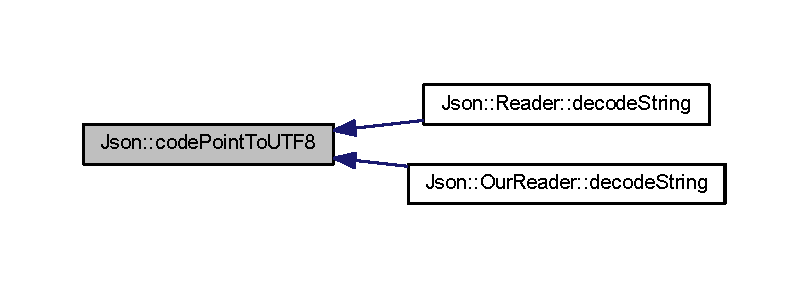
\includegraphics[width=350pt]{namespace_json_a33f8bda65a5b1fc4f5ddc39cb03dc742_icgraph}
\end{center}
\end{figure}
\mbox{\Hypertarget{namespace_json_aa11b210ff98a4f4dd4e2df19260f8c3a}\label{namespace_json_aa11b210ff98a4f4dd4e2df19260f8c3a}} 
\index{Json@{Json}!contains\+Control\+Character@{contains\+Control\+Character}}
\index{contains\+Control\+Character@{contains\+Control\+Character}!Json@{Json}}
\subsubsection{\texorpdfstring{contains\+Control\+Character()}{containsControlCharacter()}}
{\footnotesize\ttfamily static bool Json\+::contains\+Control\+Character (\begin{DoxyParamCaption}\item[{const char $\ast$}]{str }\end{DoxyParamCaption})\hspace{0.3cm}{\ttfamily [static]}}



jsoncpp.\+cpp 파일의 4163 번째 라인에서 정의되었습니다.


\begin{DoxyCode}
4163                                                       \{
4164   \textcolor{keywordflow}{while} (*str) \{
4165     \textcolor{keywordflow}{if} (\hyperlink{namespace_json_a0381e631737f51331065a388f4f59197}{isControlCharacter}(*(str++)))
4166       \textcolor{keywordflow}{return} \textcolor{keyword}{true};
4167   \}
4168   \textcolor{keywordflow}{return} \textcolor{keyword}{false};
4169 \}
\end{DoxyCode}
이 함수 내부에서 호출하는 함수들에 대한 그래프입니다.\+:\nopagebreak
\begin{figure}[H]
\begin{center}
\leavevmode
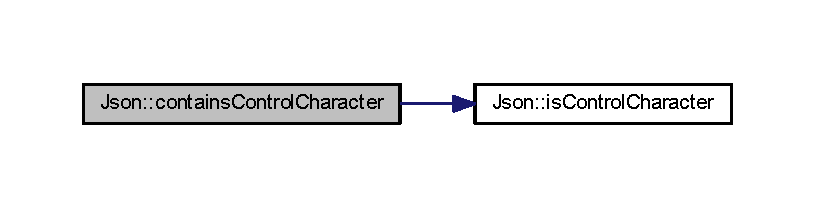
\includegraphics[width=350pt]{namespace_json_aa11b210ff98a4f4dd4e2df19260f8c3a_cgraph}
\end{center}
\end{figure}
이 함수를 호출하는 함수들에 대한 그래프입니다.\+:\nopagebreak
\begin{figure}[H]
\begin{center}
\leavevmode
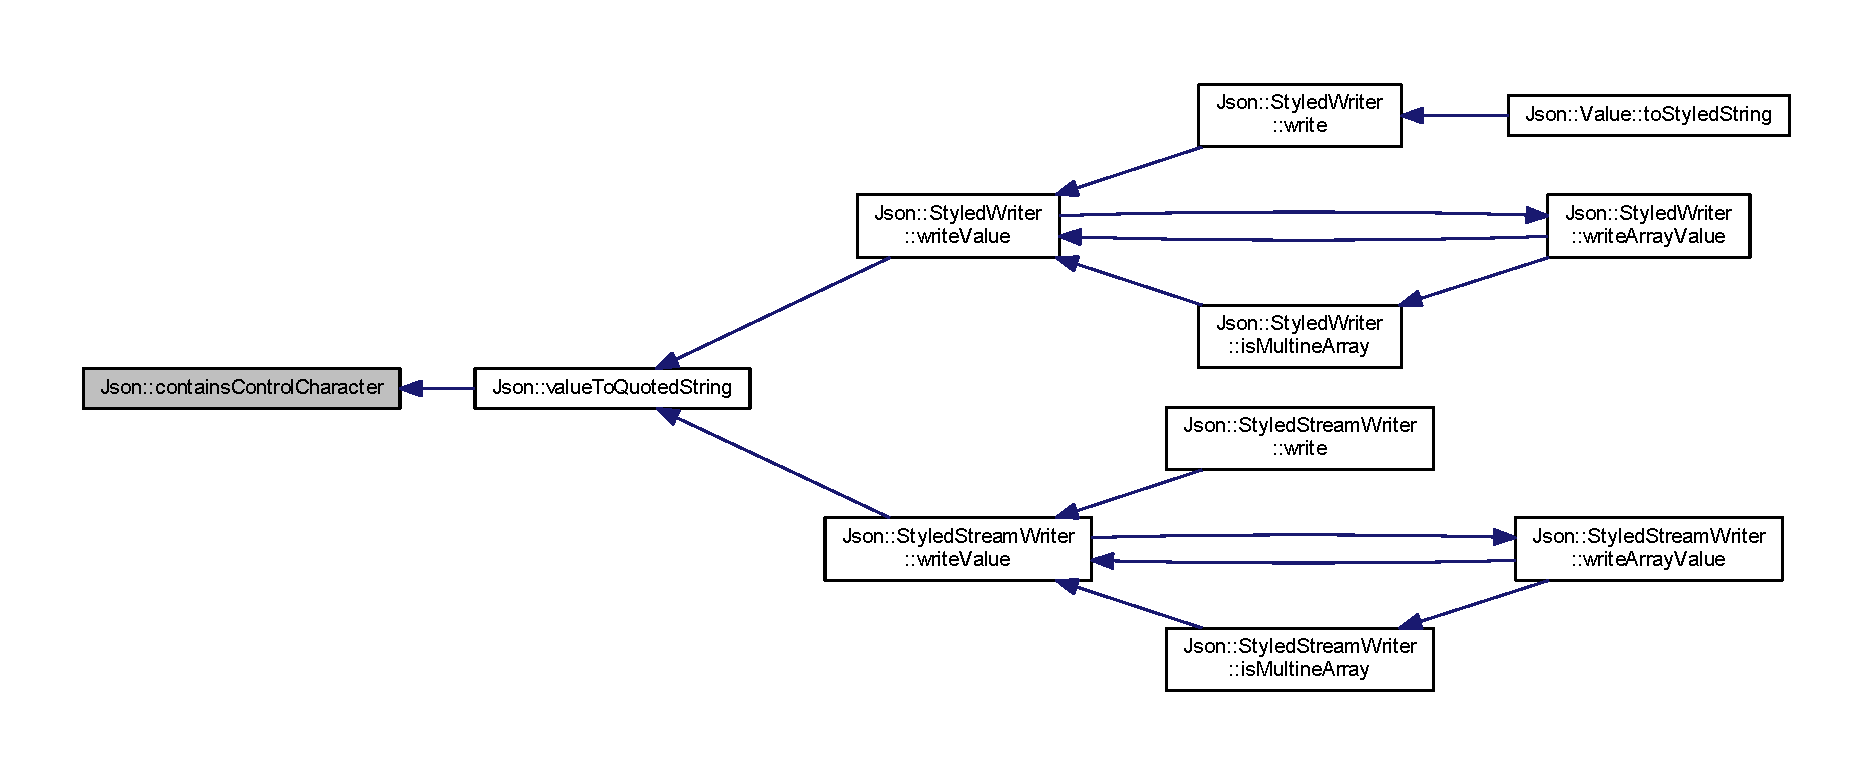
\includegraphics[width=350pt]{namespace_json_aa11b210ff98a4f4dd4e2df19260f8c3a_icgraph}
\end{center}
\end{figure}
\mbox{\Hypertarget{namespace_json_ae8a357381f264cf28f46449e79ab1dea}\label{namespace_json_ae8a357381f264cf28f46449e79ab1dea}} 
\index{Json@{Json}!contains\+Control\+Character0@{contains\+Control\+Character0}}
\index{contains\+Control\+Character0@{contains\+Control\+Character0}!Json@{Json}}
\subsubsection{\texorpdfstring{contains\+Control\+Character0()}{containsControlCharacter0()}}
{\footnotesize\ttfamily static bool Json\+::contains\+Control\+Character0 (\begin{DoxyParamCaption}\item[{const char $\ast$}]{str,  }\item[{unsigned}]{len }\end{DoxyParamCaption})\hspace{0.3cm}{\ttfamily [static]}}



jsoncpp.\+cpp 파일의 4171 번째 라인에서 정의되었습니다.


\begin{DoxyCode}
4171                                                                      \{
4172   \textcolor{keywordtype}{char} \textcolor{keyword}{const}* end = str + len;
4173   \textcolor{keywordflow}{while} (end != str) \{
4174     \textcolor{keywordflow}{if} (\hyperlink{namespace_json_a0381e631737f51331065a388f4f59197}{isControlCharacter}(*str) || 0==*str)
4175       \textcolor{keywordflow}{return} \textcolor{keyword}{true};
4176     ++str;
4177   \}
4178   \textcolor{keywordflow}{return} \textcolor{keyword}{false};
4179 \}
\end{DoxyCode}
이 함수 내부에서 호출하는 함수들에 대한 그래프입니다.\+:\nopagebreak
\begin{figure}[H]
\begin{center}
\leavevmode
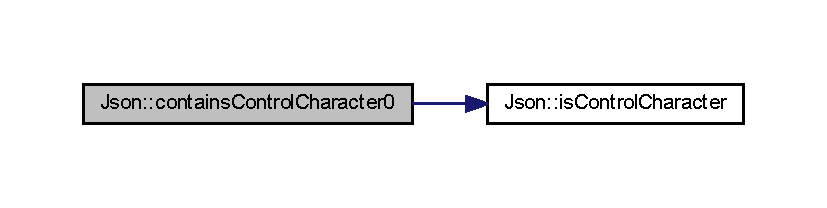
\includegraphics[width=350pt]{namespace_json_ae8a357381f264cf28f46449e79ab1dea_cgraph}
\end{center}
\end{figure}
이 함수를 호출하는 함수들에 대한 그래프입니다.\+:\nopagebreak
\begin{figure}[H]
\begin{center}
\leavevmode
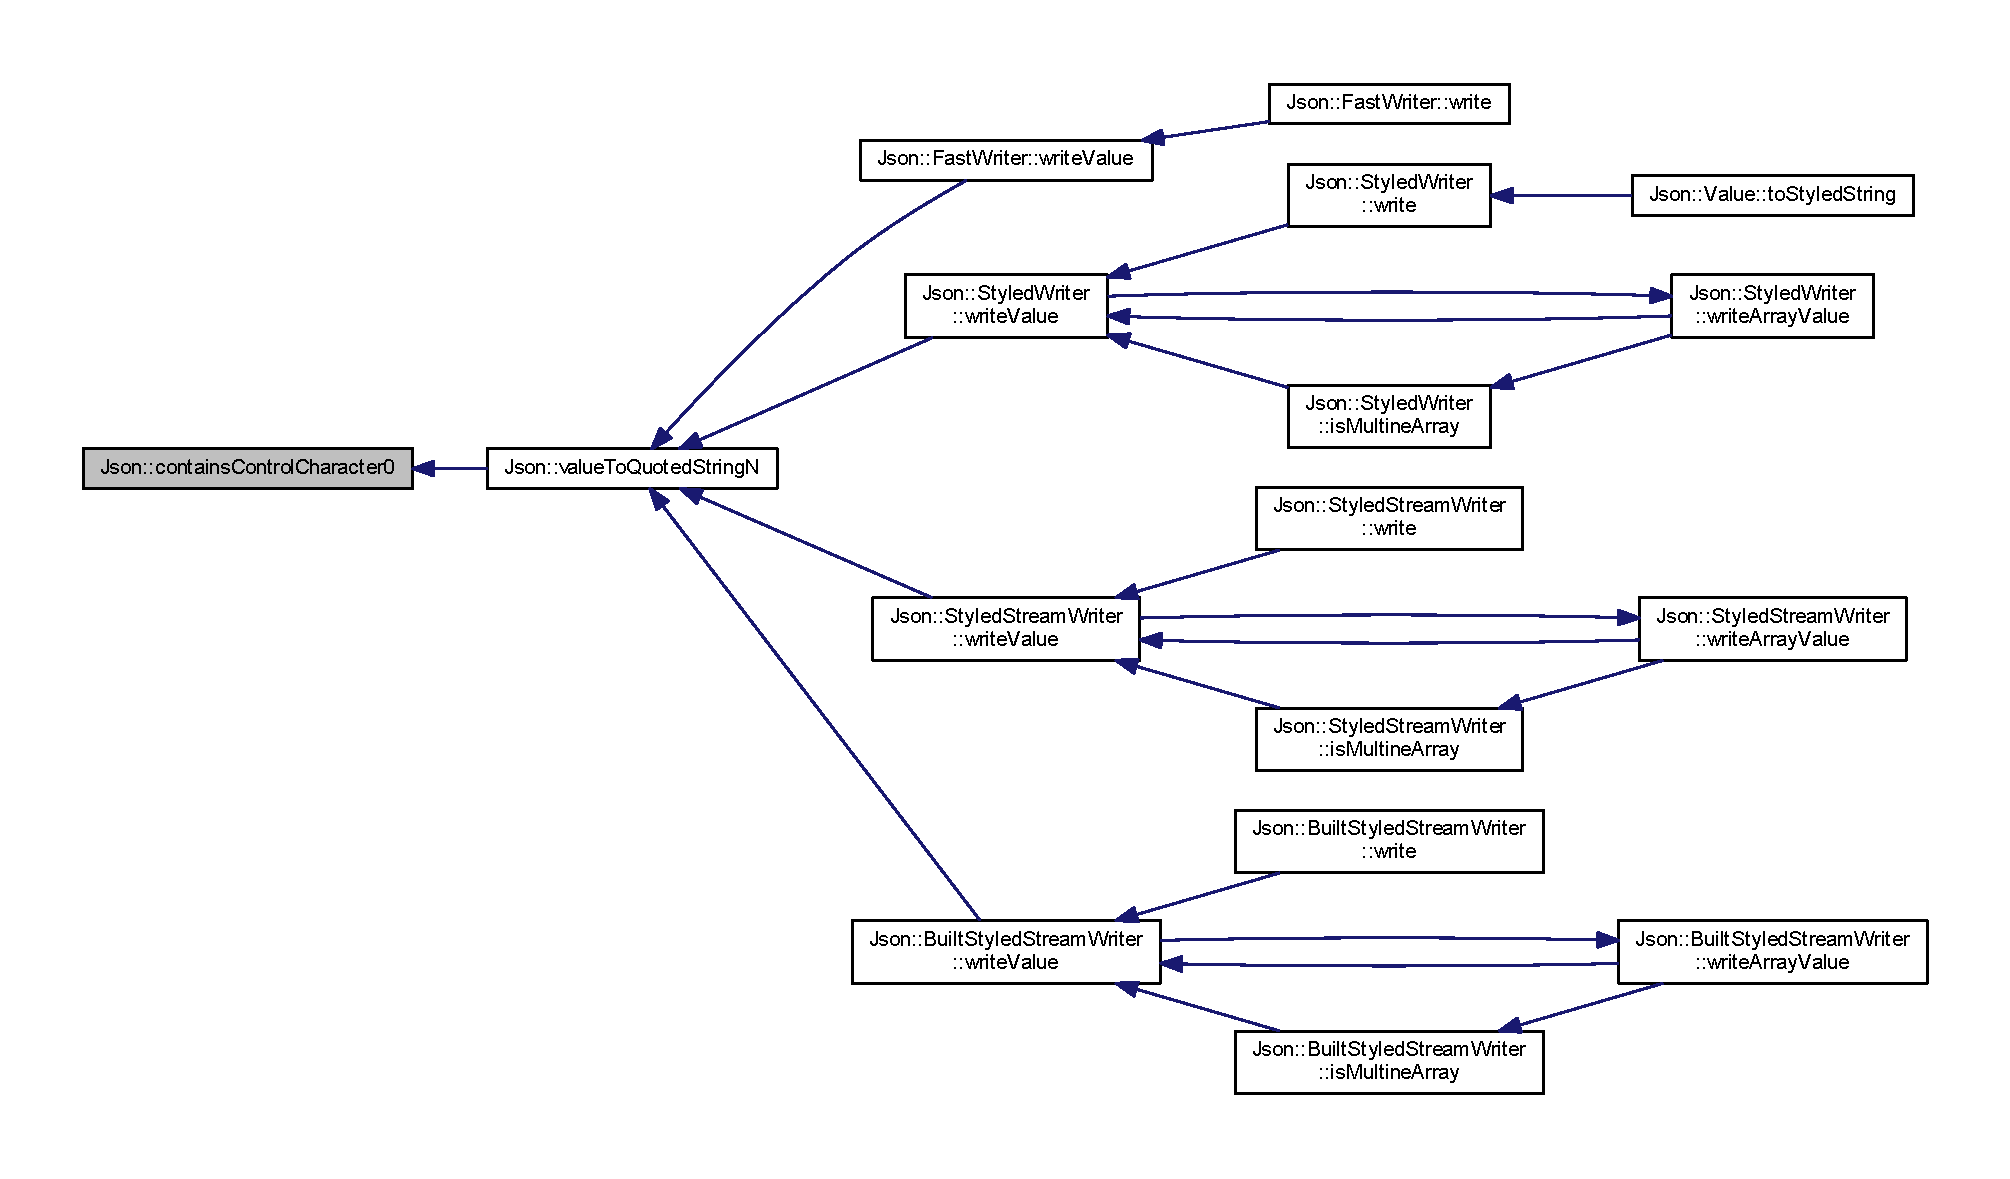
\includegraphics[width=350pt]{namespace_json_ae8a357381f264cf28f46449e79ab1dea_icgraph}
\end{center}
\end{figure}
\mbox{\Hypertarget{namespace_json_a4d6ab0f651348832e5cc49b577a854d2}\label{namespace_json_a4d6ab0f651348832e5cc49b577a854d2}} 
\index{Json@{Json}!contains\+New\+Line@{contains\+New\+Line}}
\index{contains\+New\+Line@{contains\+New\+Line}!Json@{Json}}
\subsubsection{\texorpdfstring{contains\+New\+Line()}{containsNewLine()}}
{\footnotesize\ttfamily static bool Json\+::contains\+New\+Line (\begin{DoxyParamCaption}\item[{\hyperlink{class_json_1_1_reader_a46795b5b272bf79a7730e406cb96375a}{Reader\+::\+Location}}]{begin,  }\item[{\hyperlink{class_json_1_1_reader_a46795b5b272bf79a7730e406cb96375a}{Reader\+::\+Location}}]{end }\end{DoxyParamCaption})\hspace{0.3cm}{\ttfamily [static]}}



jsoncpp.\+cpp 파일의 301 번째 라인에서 정의되었습니다.


\begin{DoxyCode}
301                                                                       \{
302   \textcolor{keywordflow}{for} (; begin < end; ++begin)
303     \textcolor{keywordflow}{if} (*begin == \textcolor{charliteral}{'\(\backslash\)n'} || *begin == \textcolor{charliteral}{'\(\backslash\)r'})
304       \textcolor{keywordflow}{return} \textcolor{keyword}{true};
305   \textcolor{keywordflow}{return} \textcolor{keyword}{false};
306 \}
\end{DoxyCode}
이 함수를 호출하는 함수들에 대한 그래프입니다.\+:\nopagebreak
\begin{figure}[H]
\begin{center}
\leavevmode
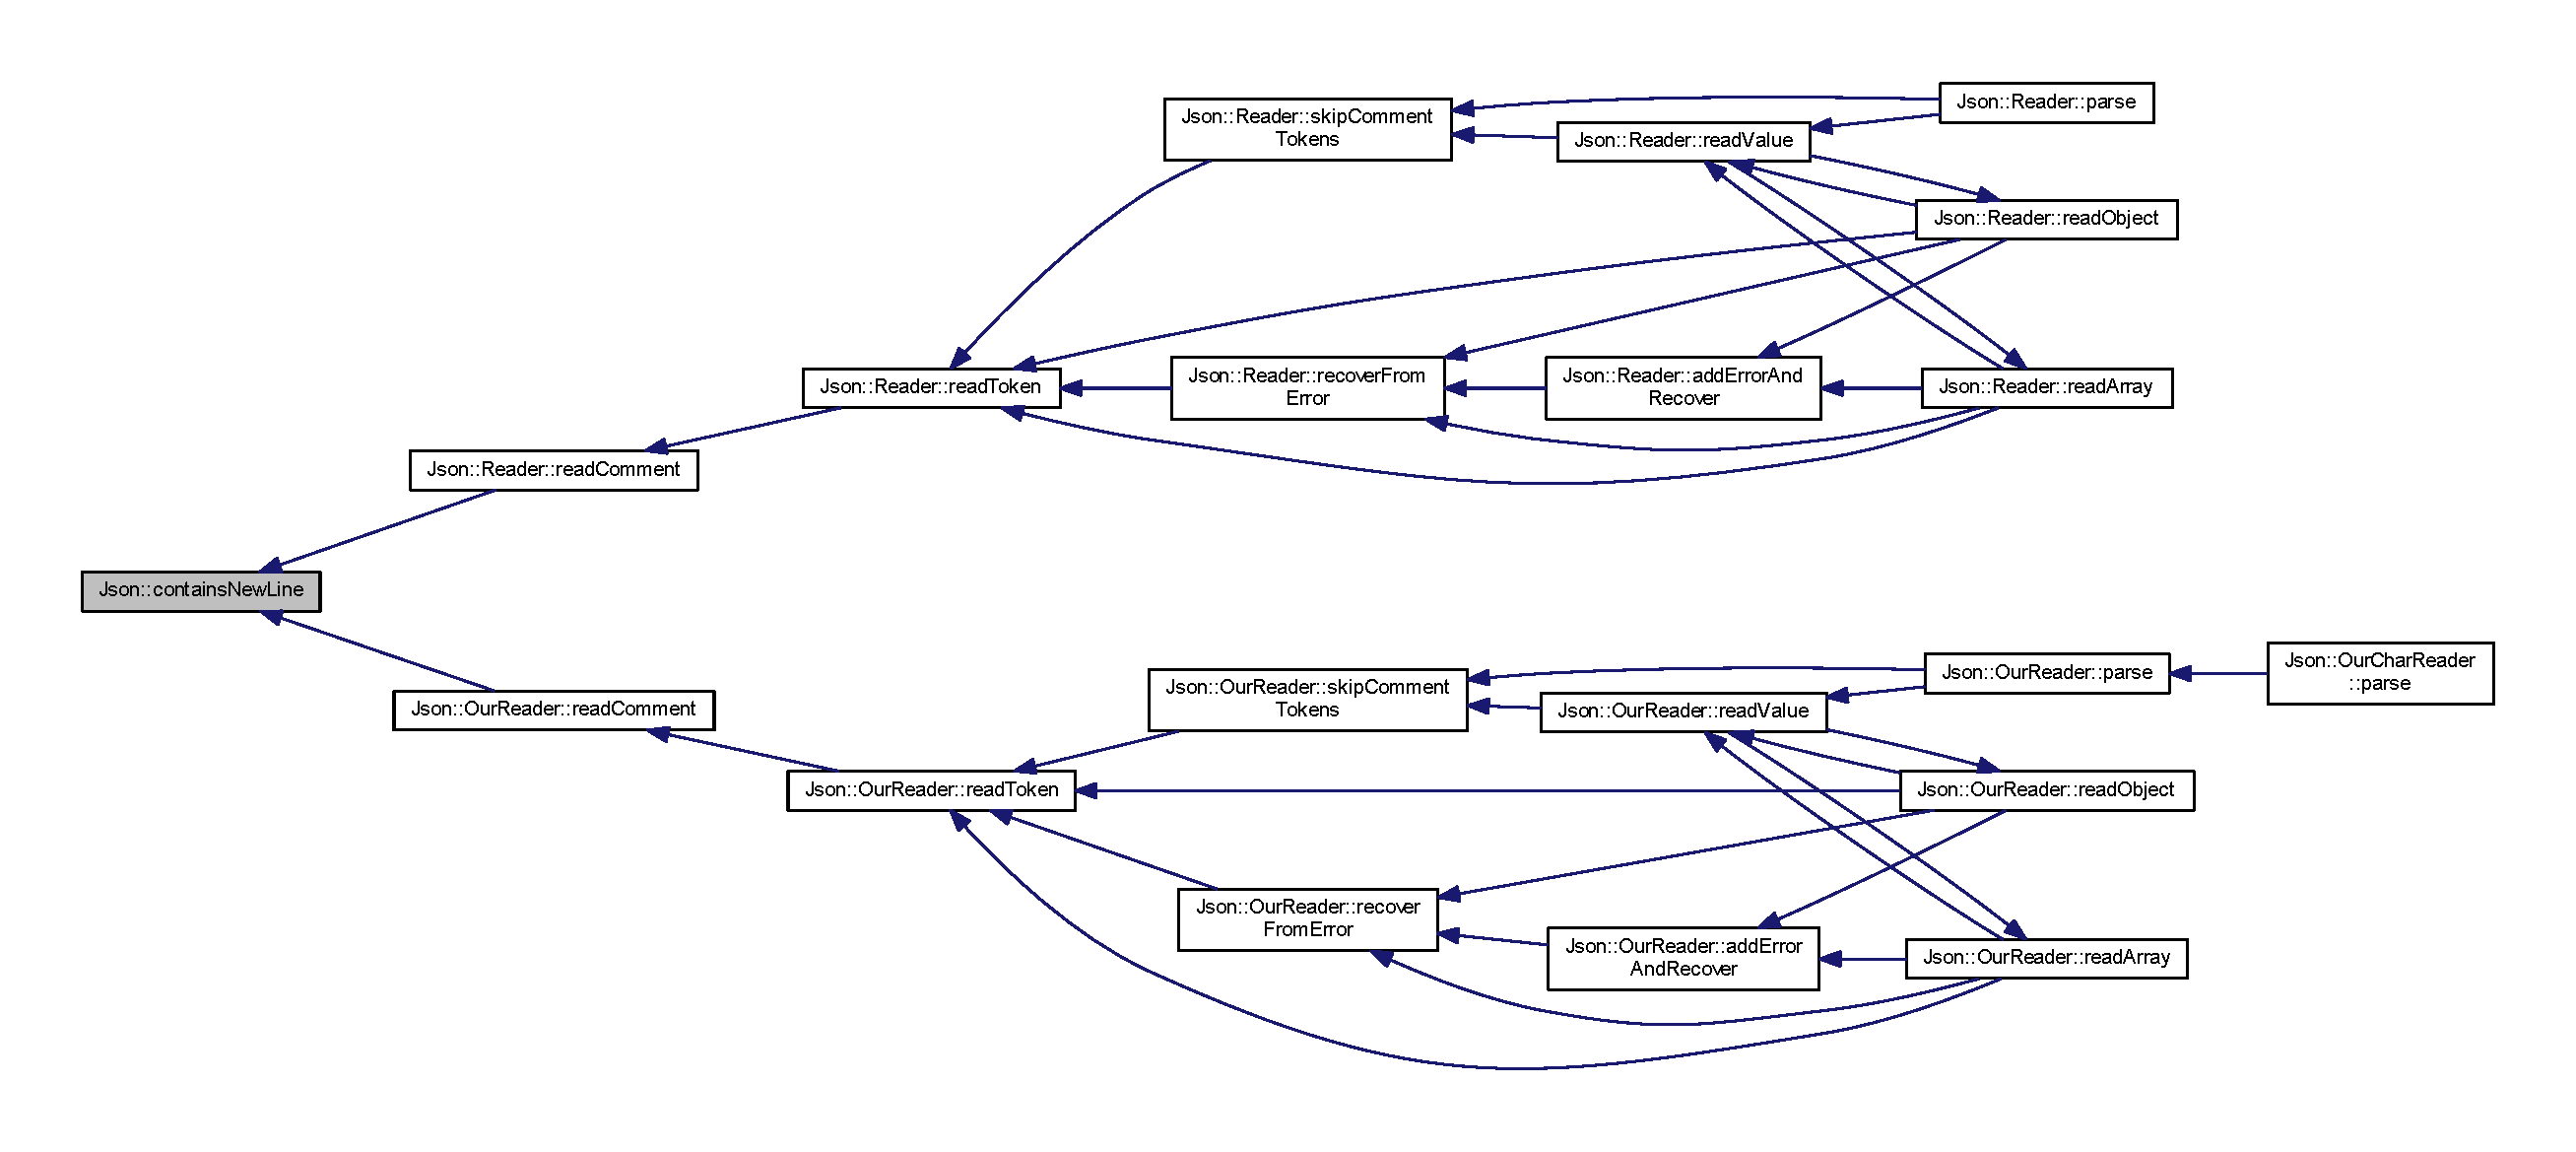
\includegraphics[width=350pt]{namespace_json_a4d6ab0f651348832e5cc49b577a854d2_icgraph}
\end{center}
\end{figure}
\mbox{\Hypertarget{namespace_json_aad8b4982c1acd164f541fba396ac9fb1}\label{namespace_json_aad8b4982c1acd164f541fba396ac9fb1}} 
\index{Json@{Json}!decode\+Prefixed\+String@{decode\+Prefixed\+String}}
\index{decode\+Prefixed\+String@{decode\+Prefixed\+String}!Json@{Json}}
\subsubsection{\texorpdfstring{decode\+Prefixed\+String()}{decodePrefixedString()}}
{\footnotesize\ttfamily static void Json\+::decode\+Prefixed\+String (\begin{DoxyParamCaption}\item[{bool}]{is\+Prefixed,  }\item[{char const $\ast$}]{prefixed,  }\item[{unsigned $\ast$}]{length,  }\item[{char const $\ast$$\ast$}]{value }\end{DoxyParamCaption})\hspace{0.3cm}{\ttfamily [inline]}, {\ttfamily [static]}}



jsoncpp.\+cpp 파일의 2587 번째 라인에서 정의되었습니다.


\begin{DoxyCode}
2590 \{
2591   \textcolor{keywordflow}{if} (!isPrefixed) \{
2592     *length = \textcolor{keyword}{static\_cast<}\textcolor{keywordtype}{unsigned}\textcolor{keyword}{>}(strlen(prefixed));
2593     *value = prefixed;
2594   \} \textcolor{keywordflow}{else} \{
2595     *length = *\textcolor{keyword}{reinterpret\_cast<}\textcolor{keywordtype}{unsigned} const*\textcolor{keyword}{>}(prefixed);
2596     *value = prefixed + \textcolor{keyword}{sizeof}(unsigned);
2597   \}
2598 \}
\end{DoxyCode}
이 함수 내부에서 호출하는 함수들에 대한 그래프입니다.\+:\nopagebreak
\begin{figure}[H]
\begin{center}
\leavevmode
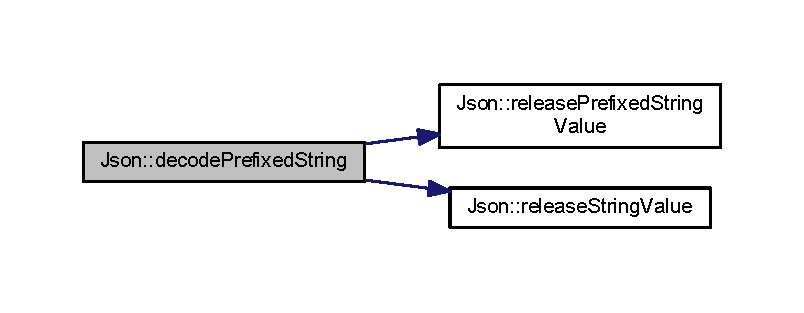
\includegraphics[width=350pt]{namespace_json_aad8b4982c1acd164f541fba396ac9fb1_cgraph}
\end{center}
\end{figure}
이 함수를 호출하는 함수들에 대한 그래프입니다.\+:\nopagebreak
\begin{figure}[H]
\begin{center}
\leavevmode
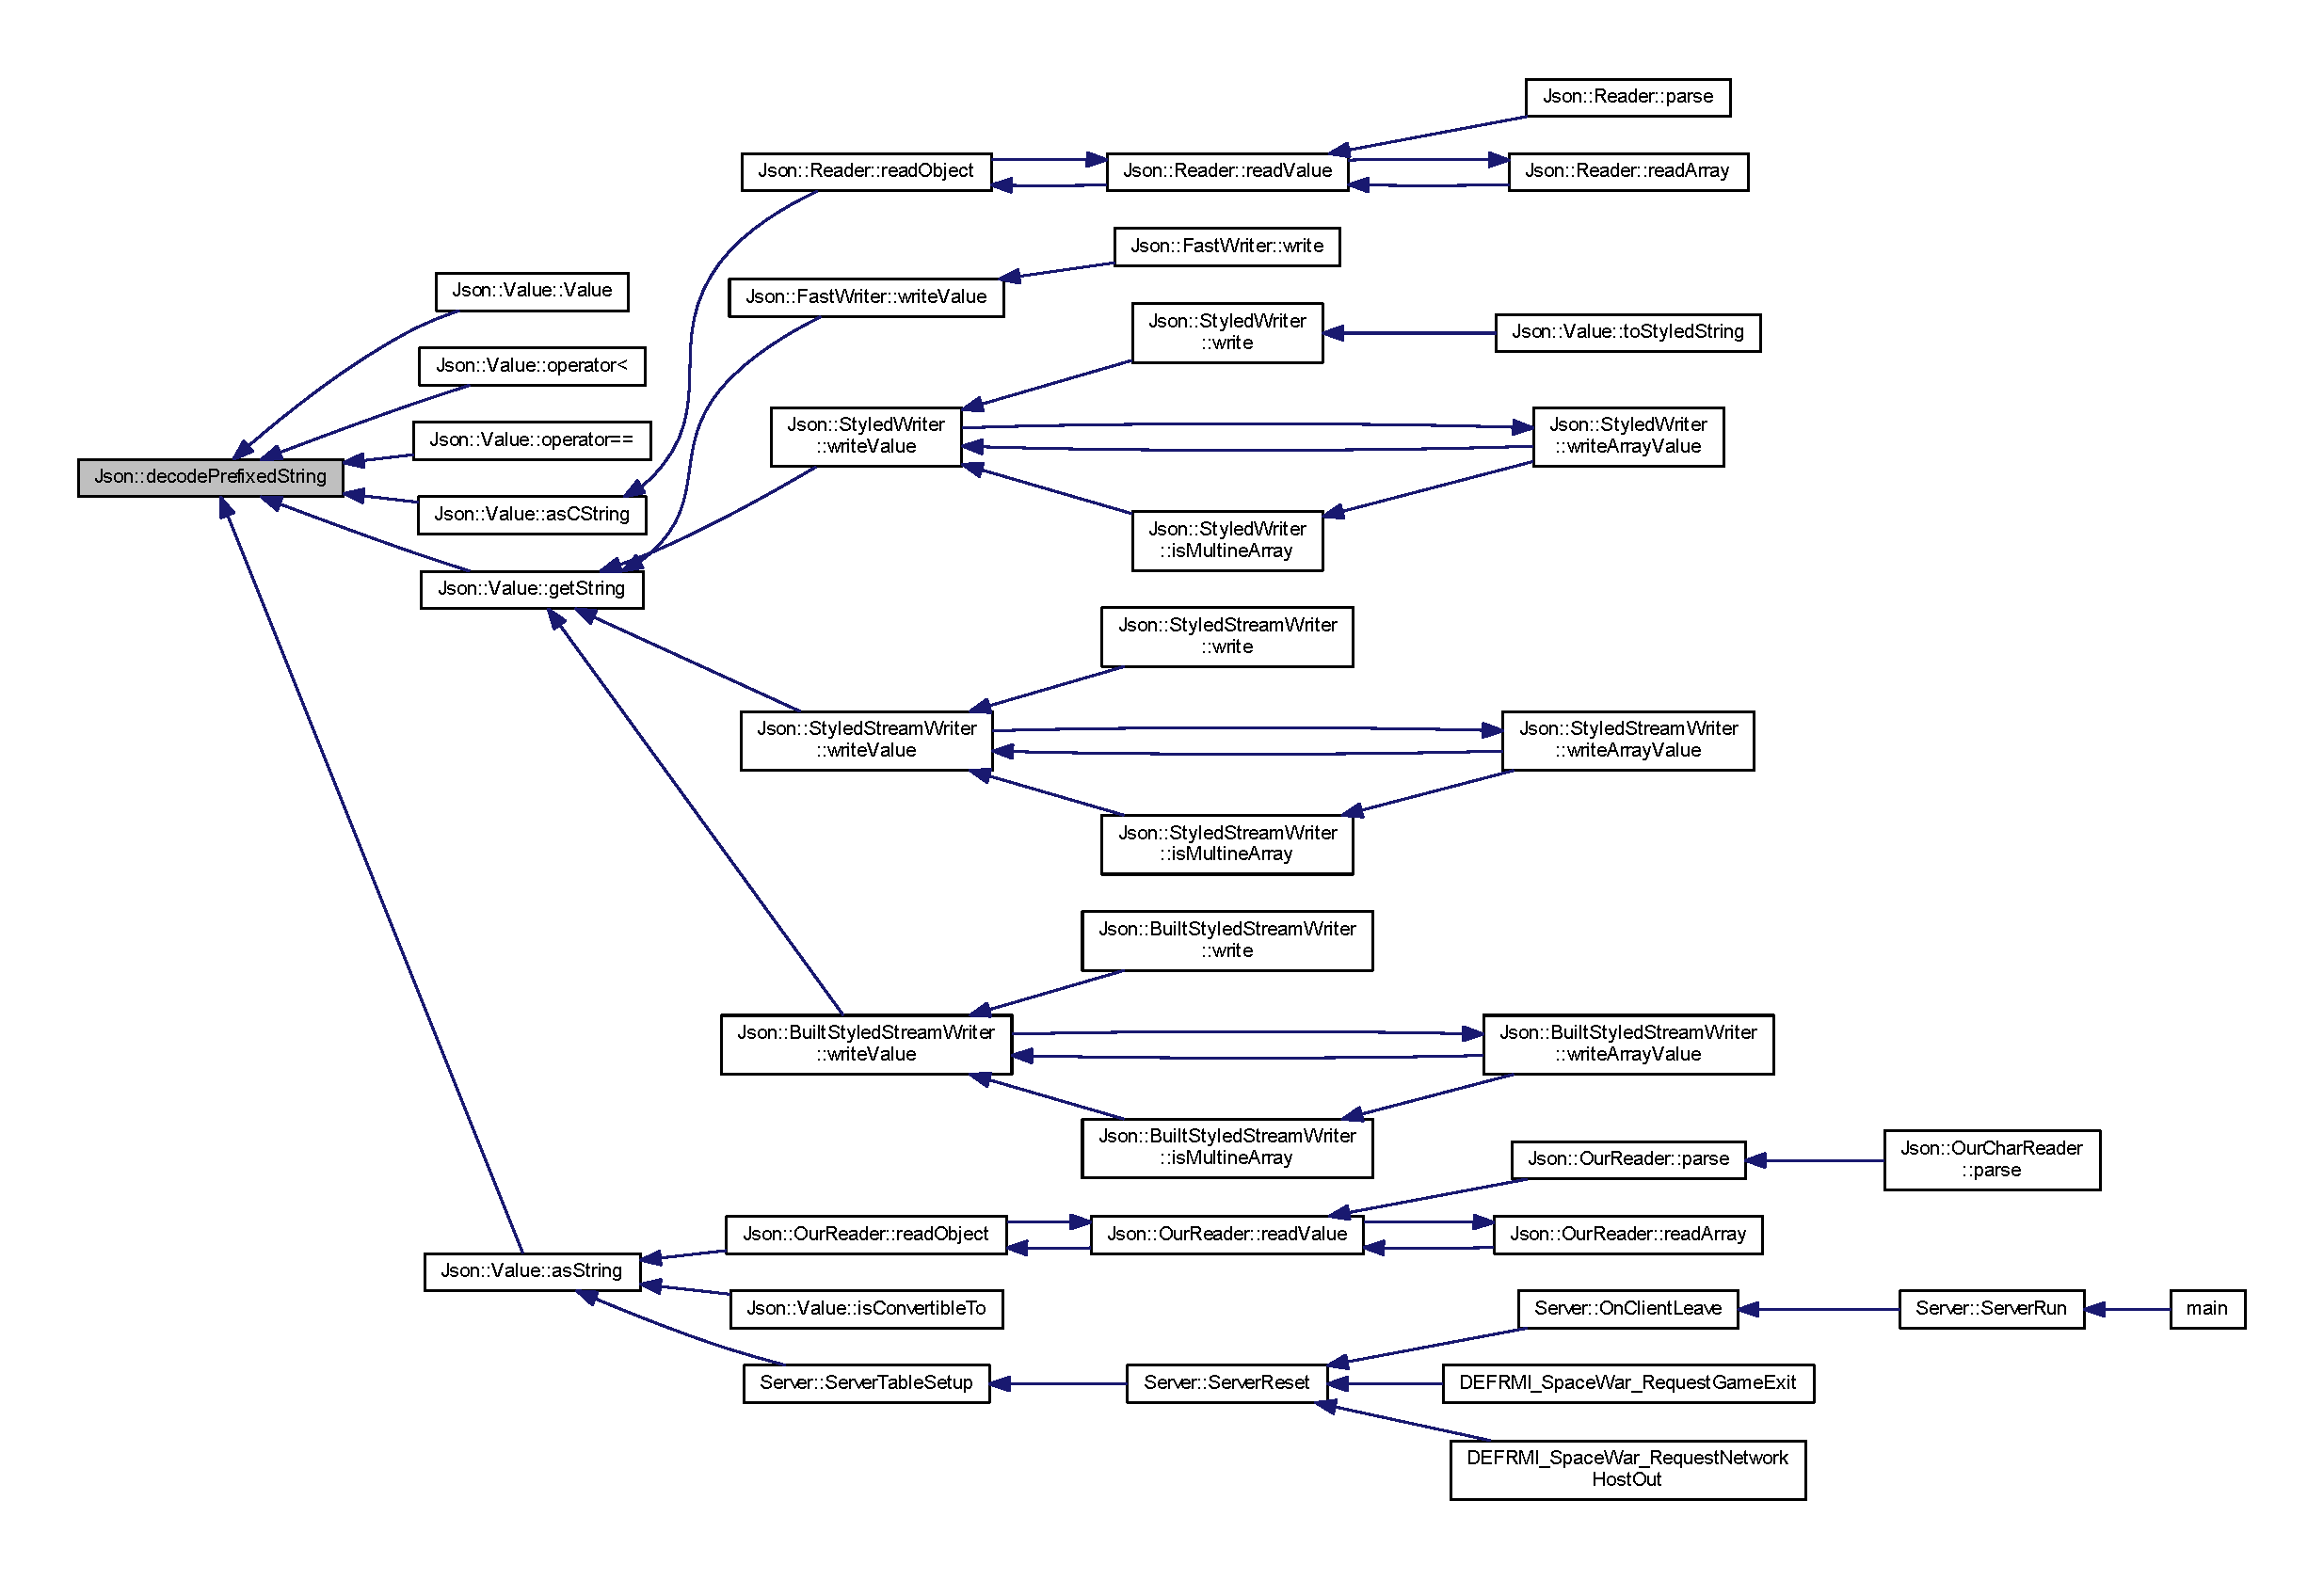
\includegraphics[width=350pt]{namespace_json_aad8b4982c1acd164f541fba396ac9fb1_icgraph}
\end{center}
\end{figure}
\mbox{\Hypertarget{namespace_json_a9795a09a0141d1f12d307c4386aeaee6}\label{namespace_json_a9795a09a0141d1f12d307c4386aeaee6}} 
\index{Json@{Json}!duplicate\+And\+Prefix\+String\+Value@{duplicate\+And\+Prefix\+String\+Value}}
\index{duplicate\+And\+Prefix\+String\+Value@{duplicate\+And\+Prefix\+String\+Value}!Json@{Json}}
\subsubsection{\texorpdfstring{duplicate\+And\+Prefix\+String\+Value()}{duplicateAndPrefixStringValue()}}
{\footnotesize\ttfamily static char$\ast$ Json\+::duplicate\+And\+Prefix\+String\+Value (\begin{DoxyParamCaption}\item[{const char $\ast$}]{value,  }\item[{unsigned int}]{length }\end{DoxyParamCaption})\hspace{0.3cm}{\ttfamily [inline]}, {\ttfamily [static]}}



jsoncpp.\+cpp 파일의 2566 번째 라인에서 정의되었습니다.


\begin{DoxyCode}
2569 \{
2570   \textcolor{comment}{// Avoid an integer overflow in the call to malloc below by limiting length}
2571   \textcolor{comment}{// to a sane value.}
2572   \hyperlink{json_8h_ad7facdeeca0f495765e3b204c265eadb}{JSON\_ASSERT\_MESSAGE}(length <= static\_cast<unsigned>(Value::maxInt) - \textcolor{keyword}{sizeof}(\textcolor{keywordtype}{unsigned}) 
      - 1U,
2573                       \textcolor{stringliteral}{"in Json::Value::duplicateAndPrefixStringValue(): "}
2574                       \textcolor{stringliteral}{"length too big for prefixing"});
2575   \textcolor{keywordtype}{unsigned} actualLength = length + \textcolor{keyword}{static\_cast<}\textcolor{keywordtype}{unsigned}\textcolor{keyword}{>}(\textcolor{keyword}{sizeof}(unsigned)) + 1U;
2576   \textcolor{keywordtype}{char}* newString = \textcolor{keyword}{static\_cast<}\textcolor{keywordtype}{char}*\textcolor{keyword}{>}(malloc(actualLength));
2577   \textcolor{keywordflow}{if} (newString == 0) \{
2578     \hyperlink{namespace_json_a0ab7ff7f99788262d92d9ff3d924e065}{throwRuntimeError}(
2579         \textcolor{stringliteral}{"in Json::Value::duplicateAndPrefixStringValue(): "}
2580         \textcolor{stringliteral}{"Failed to allocate string value buffer"});
2581   \}
2582   *\textcolor{keyword}{reinterpret\_cast<}\textcolor{keywordtype}{unsigned}*\textcolor{keyword}{>}(newString) = length;
2583   memcpy(newString + \textcolor{keyword}{sizeof}(\textcolor{keywordtype}{unsigned}), value, length);
2584   newString[actualLength - 1U] = 0; \textcolor{comment}{// to avoid buffer over-run accidents by users later}
2585   \textcolor{keywordflow}{return} newString;
2586 \}
\end{DoxyCode}
이 함수 내부에서 호출하는 함수들에 대한 그래프입니다.\+:\nopagebreak
\begin{figure}[H]
\begin{center}
\leavevmode
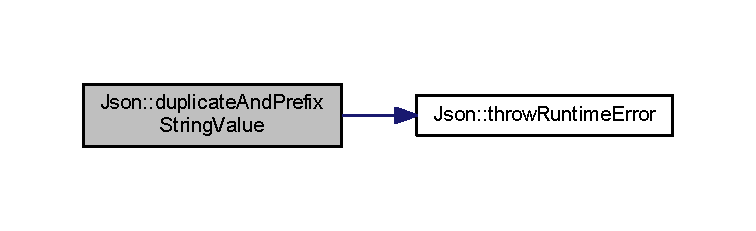
\includegraphics[width=350pt]{namespace_json_a9795a09a0141d1f12d307c4386aeaee6_cgraph}
\end{center}
\end{figure}
이 함수를 호출하는 함수들에 대한 그래프입니다.\+:\nopagebreak
\begin{figure}[H]
\begin{center}
\leavevmode
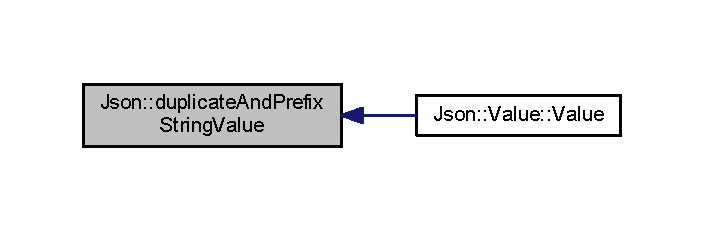
\includegraphics[width=338pt]{namespace_json_a9795a09a0141d1f12d307c4386aeaee6_icgraph}
\end{center}
\end{figure}
\mbox{\Hypertarget{namespace_json_a678ac3a60cd70ec0fb4c9abfd40eb0c4}\label{namespace_json_a678ac3a60cd70ec0fb4c9abfd40eb0c4}} 
\index{Json@{Json}!duplicate\+String\+Value@{duplicate\+String\+Value}}
\index{duplicate\+String\+Value@{duplicate\+String\+Value}!Json@{Json}}
\subsubsection{\texorpdfstring{duplicate\+String\+Value()}{duplicateStringValue()}}
{\footnotesize\ttfamily static char$\ast$ Json\+::duplicate\+String\+Value (\begin{DoxyParamCaption}\item[{const char $\ast$}]{value,  }\item[{size\+\_\+t}]{length }\end{DoxyParamCaption})\hspace{0.3cm}{\ttfamily [inline]}, {\ttfamily [static]}}

Duplicates the specified string value. 
\begin{DoxyParams}{매개변수}
{\em value} & Pointer to the string to duplicate. Must be zero-\/terminated if length is \char`\"{}unknown\char`\"{}. \\
\hline
{\em length} & Length of the value. if equals to unknown, then it will be computed using strlen(value). \\
\hline
\end{DoxyParams}
\begin{DoxyReturn}{반환값}
Pointer on the duplicate instance of string. 
\end{DoxyReturn}


jsoncpp.\+cpp 파일의 2545 번째 라인에서 정의되었습니다.


\begin{DoxyCode}
2547 \{
2548   \textcolor{comment}{// Avoid an integer overflow in the call to malloc below by limiting length}
2549   \textcolor{comment}{// to a sane value.}
2550   \textcolor{keywordflow}{if} (length >= static\_cast<size\_t>(Value::maxInt))
2551     length = Value::maxInt - 1;
2552 
2553   \textcolor{keywordtype}{char}* newString = \textcolor{keyword}{static\_cast<}\textcolor{keywordtype}{char}*\textcolor{keyword}{>}(malloc(length + 1));
2554   \textcolor{keywordflow}{if} (newString == NULL) \{
2555     \hyperlink{namespace_json_a0ab7ff7f99788262d92d9ff3d924e065}{throwRuntimeError}(
2556         \textcolor{stringliteral}{"in Json::Value::duplicateStringValue(): "}
2557         \textcolor{stringliteral}{"Failed to allocate string value buffer"});
2558   \}
2559   memcpy(newString, value, length);
2560   newString[length] = 0;
2561   \textcolor{keywordflow}{return} newString;
2562 \}
\end{DoxyCode}
이 함수 내부에서 호출하는 함수들에 대한 그래프입니다.\+:\nopagebreak
\begin{figure}[H]
\begin{center}
\leavevmode
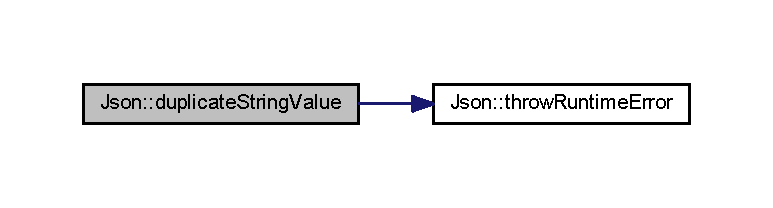
\includegraphics[width=350pt]{namespace_json_a678ac3a60cd70ec0fb4c9abfd40eb0c4_cgraph}
\end{center}
\end{figure}
이 함수를 호출하는 함수들에 대한 그래프입니다.\+:
\nopagebreak
\begin{figure}[H]
\begin{center}
\leavevmode
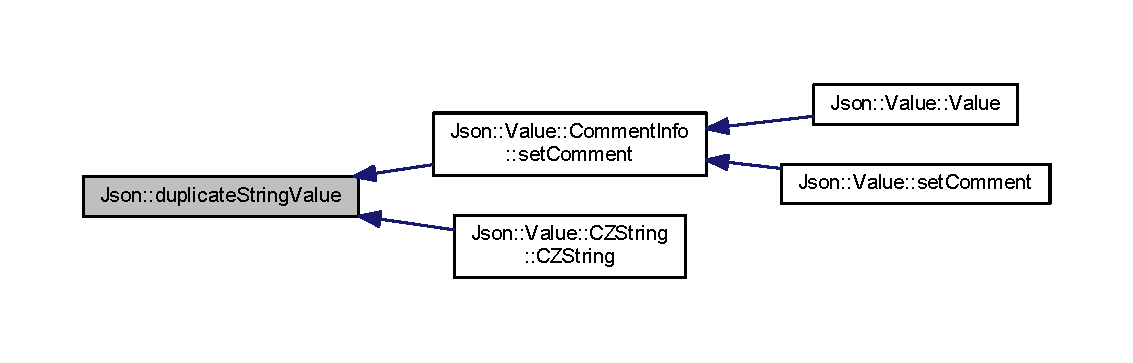
\includegraphics[width=350pt]{namespace_json_a678ac3a60cd70ec0fb4c9abfd40eb0c4_icgraph}
\end{center}
\end{figure}
\mbox{\Hypertarget{namespace_json_aa208904144dc7b11ccc28f47c9afab9a}\label{namespace_json_aa208904144dc7b11ccc28f47c9afab9a}} 
\index{Json@{Json}!fix\+Numeric\+Locale@{fix\+Numeric\+Locale}}
\index{fix\+Numeric\+Locale@{fix\+Numeric\+Locale}!Json@{Json}}
\subsubsection{\texorpdfstring{fix\+Numeric\+Locale()}{fixNumericLocale()}}
{\footnotesize\ttfamily static void Json\+::fix\+Numeric\+Locale (\begin{DoxyParamCaption}\item[{char $\ast$}]{begin,  }\item[{char $\ast$}]{end }\end{DoxyParamCaption})\hspace{0.3cm}{\ttfamily [inline]}, {\ttfamily [static]}}

Change \textquotesingle{},\textquotesingle{} to \textquotesingle{}.\textquotesingle{} everywhere in buffer.

We had a sophisticated way, but it did not work in Win\+CE. \begin{DoxySeeAlso}{참고}
\href{https://github.com/open-source-parsers/jsoncpp/pull/9}{\tt https\+://github.\+com/open-\/source-\/parsers/jsoncpp/pull/9} 
\end{DoxySeeAlso}


jsoncpp.\+cpp 파일의 180 번째 라인에서 정의되었습니다.


\begin{DoxyCode}
180                                                             \{
181   \textcolor{keywordflow}{while} (begin < end) \{
182     \textcolor{keywordflow}{if} (*begin == \textcolor{charliteral}{','}) \{
183       *begin = \textcolor{charliteral}{'.'};
184     \}
185     ++begin;
186   \}
187 \}
\end{DoxyCode}
이 함수를 호출하는 함수들에 대한 그래프입니다.\+:\nopagebreak
\begin{figure}[H]
\begin{center}
\leavevmode
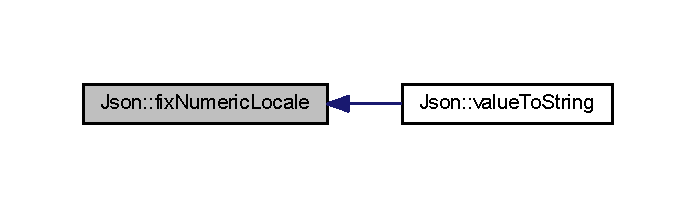
\includegraphics[width=334pt]{namespace_json_aa208904144dc7b11ccc28f47c9afab9a_icgraph}
\end{center}
\end{figure}
\mbox{\Hypertarget{namespace_json_ac142c270507391c8d86f35b550d36eb4}\label{namespace_json_ac142c270507391c8d86f35b550d36eb4}} 
\index{Json@{Json}!fix\+Numeric\+Locale\+Input@{fix\+Numeric\+Locale\+Input}}
\index{fix\+Numeric\+Locale\+Input@{fix\+Numeric\+Locale\+Input}!Json@{Json}}
\subsubsection{\texorpdfstring{fix\+Numeric\+Locale\+Input()}{fixNumericLocaleInput()}}
{\footnotesize\ttfamily static void Json\+::fix\+Numeric\+Locale\+Input (\begin{DoxyParamCaption}\item[{char $\ast$}]{begin,  }\item[{char $\ast$}]{end }\end{DoxyParamCaption})\hspace{0.3cm}{\ttfamily [inline]}, {\ttfamily [static]}}



jsoncpp.\+cpp 파일의 189 번째 라인에서 정의되었습니다.


\begin{DoxyCode}
189                                                                  \{
190   \textcolor{keywordtype}{char} decimalPoint = \hyperlink{namespace_json_ac99d7a5551039dfa712dd1d143c25a16}{getDecimalPoint}();
191   \textcolor{keywordflow}{if} (decimalPoint != \textcolor{charliteral}{'\(\backslash\)0'} && decimalPoint != \textcolor{charliteral}{'.'}) \{
192     \textcolor{keywordflow}{while} (begin < end) \{
193       \textcolor{keywordflow}{if} (*begin == \textcolor{charliteral}{'.'}) \{
194         *begin = decimalPoint;
195       \}
196       ++begin;
197     \}
198   \}
199 \}
\end{DoxyCode}
이 함수 내부에서 호출하는 함수들에 대한 그래프입니다.\+:\nopagebreak
\begin{figure}[H]
\begin{center}
\leavevmode
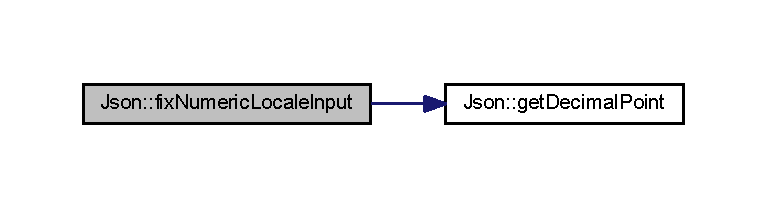
\includegraphics[width=350pt]{namespace_json_ac142c270507391c8d86f35b550d36eb4_cgraph}
\end{center}
\end{figure}
이 함수를 호출하는 함수들에 대한 그래프입니다.\+:\nopagebreak
\begin{figure}[H]
\begin{center}
\leavevmode
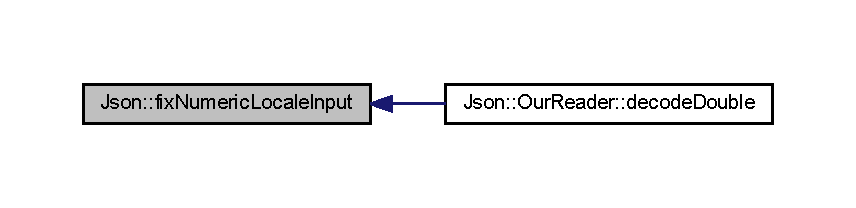
\includegraphics[width=350pt]{namespace_json_ac142c270507391c8d86f35b550d36eb4_icgraph}
\end{center}
\end{figure}
\mbox{\Hypertarget{namespace_json_ac99d7a5551039dfa712dd1d143c25a16}\label{namespace_json_ac99d7a5551039dfa712dd1d143c25a16}} 
\index{Json@{Json}!get\+Decimal\+Point@{get\+Decimal\+Point}}
\index{get\+Decimal\+Point@{get\+Decimal\+Point}!Json@{Json}}
\subsubsection{\texorpdfstring{get\+Decimal\+Point()}{getDecimalPoint()}}
{\footnotesize\ttfamily static char Json\+::get\+Decimal\+Point (\begin{DoxyParamCaption}{ }\end{DoxyParamCaption})\hspace{0.3cm}{\ttfamily [static]}}



jsoncpp.\+cpp 파일의 112 번째 라인에서 정의되었습니다.


\begin{DoxyCode}
112                               \{
113 \textcolor{preprocessor}{#ifdef JSONCPP\_NO\_LOCALE\_SUPPORT}
114   \textcolor{keywordflow}{return} \textcolor{charliteral}{'\(\backslash\)0'};
115 \textcolor{preprocessor}{#else}
116   \textcolor{keyword}{struct }lconv* lc = localeconv();
117   \textcolor{keywordflow}{return} lc ? *(lc->decimal\_point) : \textcolor{charliteral}{'\(\backslash\)0'};
118 \textcolor{preprocessor}{#endif}
119 \}
\end{DoxyCode}
이 함수를 호출하는 함수들에 대한 그래프입니다.\+:\nopagebreak
\begin{figure}[H]
\begin{center}
\leavevmode
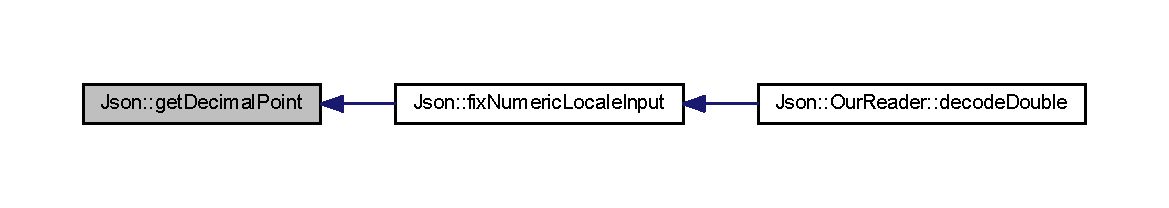
\includegraphics[width=350pt]{namespace_json_ac99d7a5551039dfa712dd1d143c25a16_icgraph}
\end{center}
\end{figure}
\mbox{\Hypertarget{namespace_json_a8c38450840f3d88e9b981ae132f7ad0a}\label{namespace_json_a8c38450840f3d88e9b981ae132f7ad0a}} 
\index{Json@{Json}!get\+Valid\+Reader\+Keys@{get\+Valid\+Reader\+Keys}}
\index{get\+Valid\+Reader\+Keys@{get\+Valid\+Reader\+Keys}!Json@{Json}}
\subsubsection{\texorpdfstring{get\+Valid\+Reader\+Keys()}{getValidReaderKeys()}}
{\footnotesize\ttfamily static void Json\+::get\+Valid\+Reader\+Keys (\begin{DoxyParamCaption}\item[{std\+::set$<$ \hyperlink{json_8h_a1e723f95759de062585bc4a8fd3fa4be}{J\+S\+O\+N\+C\+P\+P\+\_\+\+S\+T\+R\+I\+NG} $>$ $\ast$}]{valid\+\_\+keys }\end{DoxyParamCaption})\hspace{0.3cm}{\ttfamily [static]}}



jsoncpp.\+cpp 파일의 2155 번째 라인에서 정의되었습니다.


\begin{DoxyCode}
2156 \{
2157   valid\_keys->clear();
2158   valid\_keys->insert(\textcolor{stringliteral}{"collectComments"});
2159   valid\_keys->insert(\textcolor{stringliteral}{"allowComments"});
2160   valid\_keys->insert(\textcolor{stringliteral}{"strictRoot"});
2161   valid\_keys->insert(\textcolor{stringliteral}{"allowDroppedNullPlaceholders"});
2162   valid\_keys->insert(\textcolor{stringliteral}{"allowNumericKeys"});
2163   valid\_keys->insert(\textcolor{stringliteral}{"allowSingleQuotes"});
2164   valid\_keys->insert(\textcolor{stringliteral}{"stackLimit"});
2165   valid\_keys->insert(\textcolor{stringliteral}{"failIfExtra"});
2166   valid\_keys->insert(\textcolor{stringliteral}{"rejectDupKeys"});
2167   valid\_keys->insert(\textcolor{stringliteral}{"allowSpecialFloats"});
2168 \}
\end{DoxyCode}
이 함수를 호출하는 함수들에 대한 그래프입니다.\+:\nopagebreak
\begin{figure}[H]
\begin{center}
\leavevmode
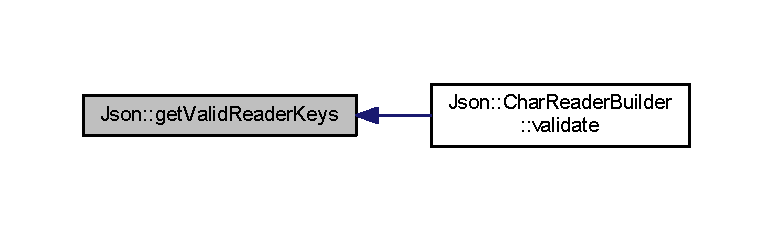
\includegraphics[width=350pt]{namespace_json_a8c38450840f3d88e9b981ae132f7ad0a_icgraph}
\end{center}
\end{figure}
\mbox{\Hypertarget{namespace_json_a77ffcc6bb405332d84c260d304d4384e}\label{namespace_json_a77ffcc6bb405332d84c260d304d4384e}} 
\index{Json@{Json}!get\+Valid\+Writer\+Keys@{get\+Valid\+Writer\+Keys}}
\index{get\+Valid\+Writer\+Keys@{get\+Valid\+Writer\+Keys}!Json@{Json}}
\subsubsection{\texorpdfstring{get\+Valid\+Writer\+Keys()}{getValidWriterKeys()}}
{\footnotesize\ttfamily static void Json\+::get\+Valid\+Writer\+Keys (\begin{DoxyParamCaption}\item[{std\+::set$<$ \hyperlink{json_8h_a1e723f95759de062585bc4a8fd3fa4be}{J\+S\+O\+N\+C\+P\+P\+\_\+\+S\+T\+R\+I\+NG} $>$ $\ast$}]{valid\+\_\+keys }\end{DoxyParamCaption})\hspace{0.3cm}{\ttfamily [static]}}



jsoncpp.\+cpp 파일의 5245 번째 라인에서 정의되었습니다.


\begin{DoxyCode}
5246 \{
5247   valid\_keys->clear();
5248   valid\_keys->insert(\textcolor{stringliteral}{"indentation"});
5249   valid\_keys->insert(\textcolor{stringliteral}{"commentStyle"});
5250   valid\_keys->insert(\textcolor{stringliteral}{"enableYAMLCompatibility"});
5251   valid\_keys->insert(\textcolor{stringliteral}{"dropNullPlaceholders"});
5252   valid\_keys->insert(\textcolor{stringliteral}{"useSpecialFloats"});
5253   valid\_keys->insert(\textcolor{stringliteral}{"precision"});
5254 \}
\end{DoxyCode}
이 함수를 호출하는 함수들에 대한 그래프입니다.\+:\nopagebreak
\begin{figure}[H]
\begin{center}
\leavevmode
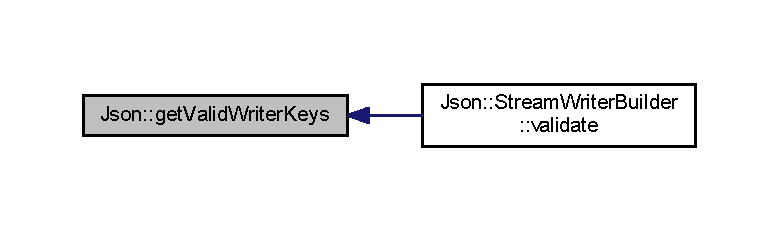
\includegraphics[width=350pt]{namespace_json_a77ffcc6bb405332d84c260d304d4384e_icgraph}
\end{center}
\end{figure}
\mbox{\Hypertarget{namespace_json_aff0180507262a244de61b961178d7443}\label{namespace_json_aff0180507262a244de61b961178d7443}} 
\index{Json@{Json}!In\+Range@{In\+Range}}
\index{In\+Range@{In\+Range}!Json@{Json}}
\subsubsection{\texorpdfstring{In\+Range()}{InRange()}}
{\footnotesize\ttfamily template$<$typename T , typename U $>$ \\
static bool Json\+::\+In\+Range (\begin{DoxyParamCaption}\item[{double}]{d,  }\item[{T}]{min,  }\item[{U}]{max }\end{DoxyParamCaption})\hspace{0.3cm}{\ttfamily [inline]}, {\ttfamily [static]}}



jsoncpp.\+cpp 파일의 2517 번째 라인에서 정의되었습니다.


\begin{DoxyCode}
2517                                                    \{
2518   \textcolor{comment}{// The casts can lose precision, but we are looking only for}
2519   \textcolor{comment}{// an approximate range. Might fail on edge cases though. ~cdunn}
2520   \textcolor{comment}{//return d >= static\_cast<double>(min) && d <= static\_cast<double>(max);}
2521   \textcolor{keywordflow}{return} d >= min && d <= max;
2522 \}
\end{DoxyCode}
이 함수를 호출하는 함수들에 대한 그래프입니다.\+:\nopagebreak
\begin{figure}[H]
\begin{center}
\leavevmode
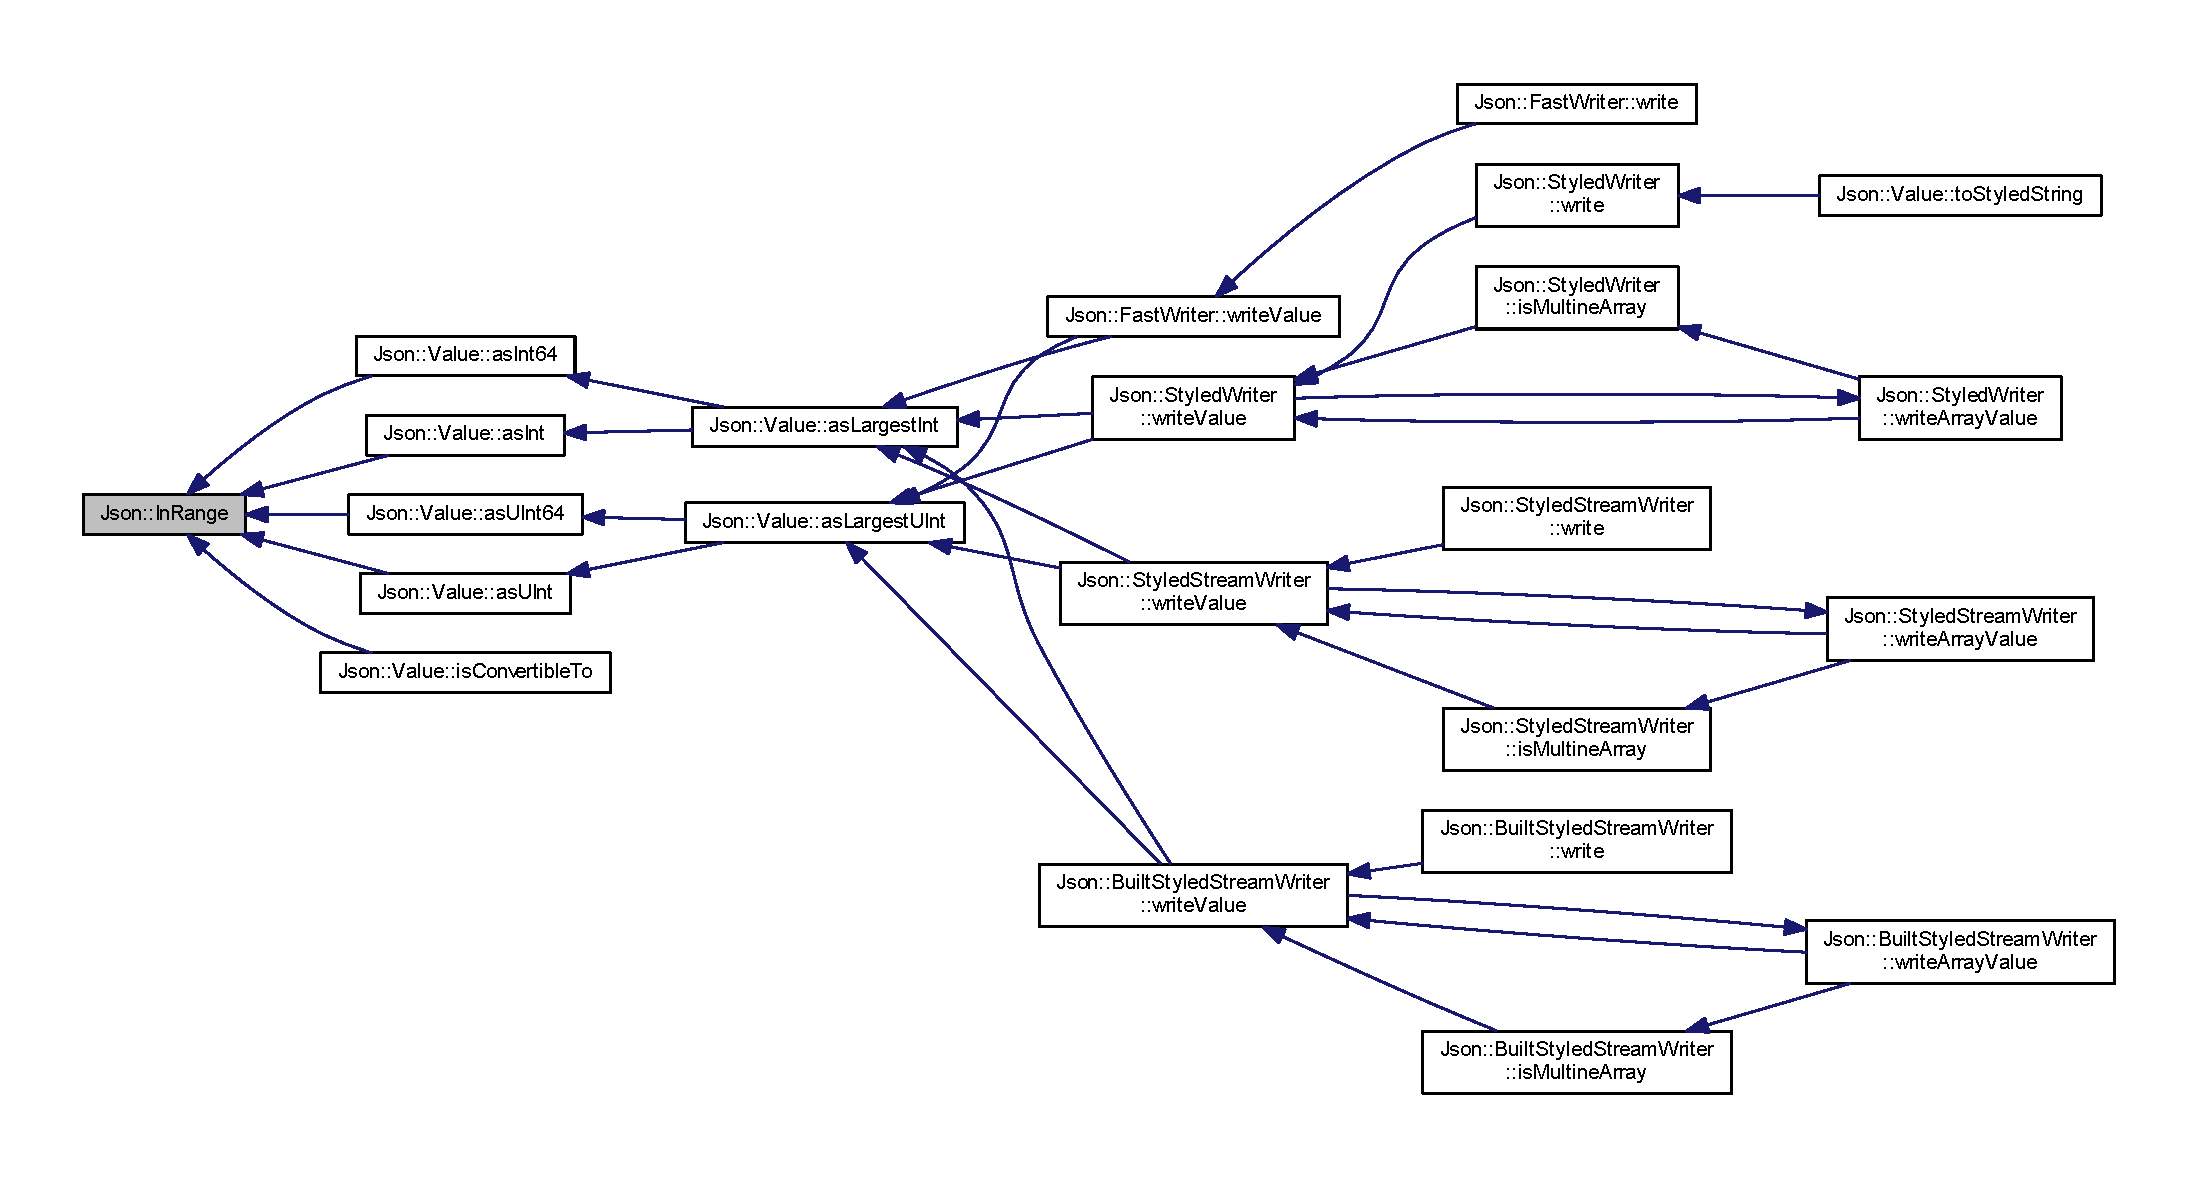
\includegraphics[width=350pt]{namespace_json_aff0180507262a244de61b961178d7443_icgraph}
\end{center}
\end{figure}
\mbox{\Hypertarget{namespace_json_a0381e631737f51331065a388f4f59197}\label{namespace_json_a0381e631737f51331065a388f4f59197}} 
\index{Json@{Json}!is\+Control\+Character@{is\+Control\+Character}}
\index{is\+Control\+Character@{is\+Control\+Character}!Json@{Json}}
\subsubsection{\texorpdfstring{is\+Control\+Character()}{isControlCharacter()}}
{\footnotesize\ttfamily static bool Json\+::is\+Control\+Character (\begin{DoxyParamCaption}\item[{char}]{ch }\end{DoxyParamCaption})\hspace{0.3cm}{\ttfamily [inline]}, {\ttfamily [static]}}



Returns true if ch is a control character (in range \mbox{[}1,31\mbox{]}). 



jsoncpp.\+cpp 파일의 151 번째 라인에서 정의되었습니다.


\begin{DoxyCode}
151 \{ \textcolor{keywordflow}{return} ch > 0 && ch <= 0x1F; \}
\end{DoxyCode}
이 함수를 호출하는 함수들에 대한 그래프입니다.\+:\nopagebreak
\begin{figure}[H]
\begin{center}
\leavevmode
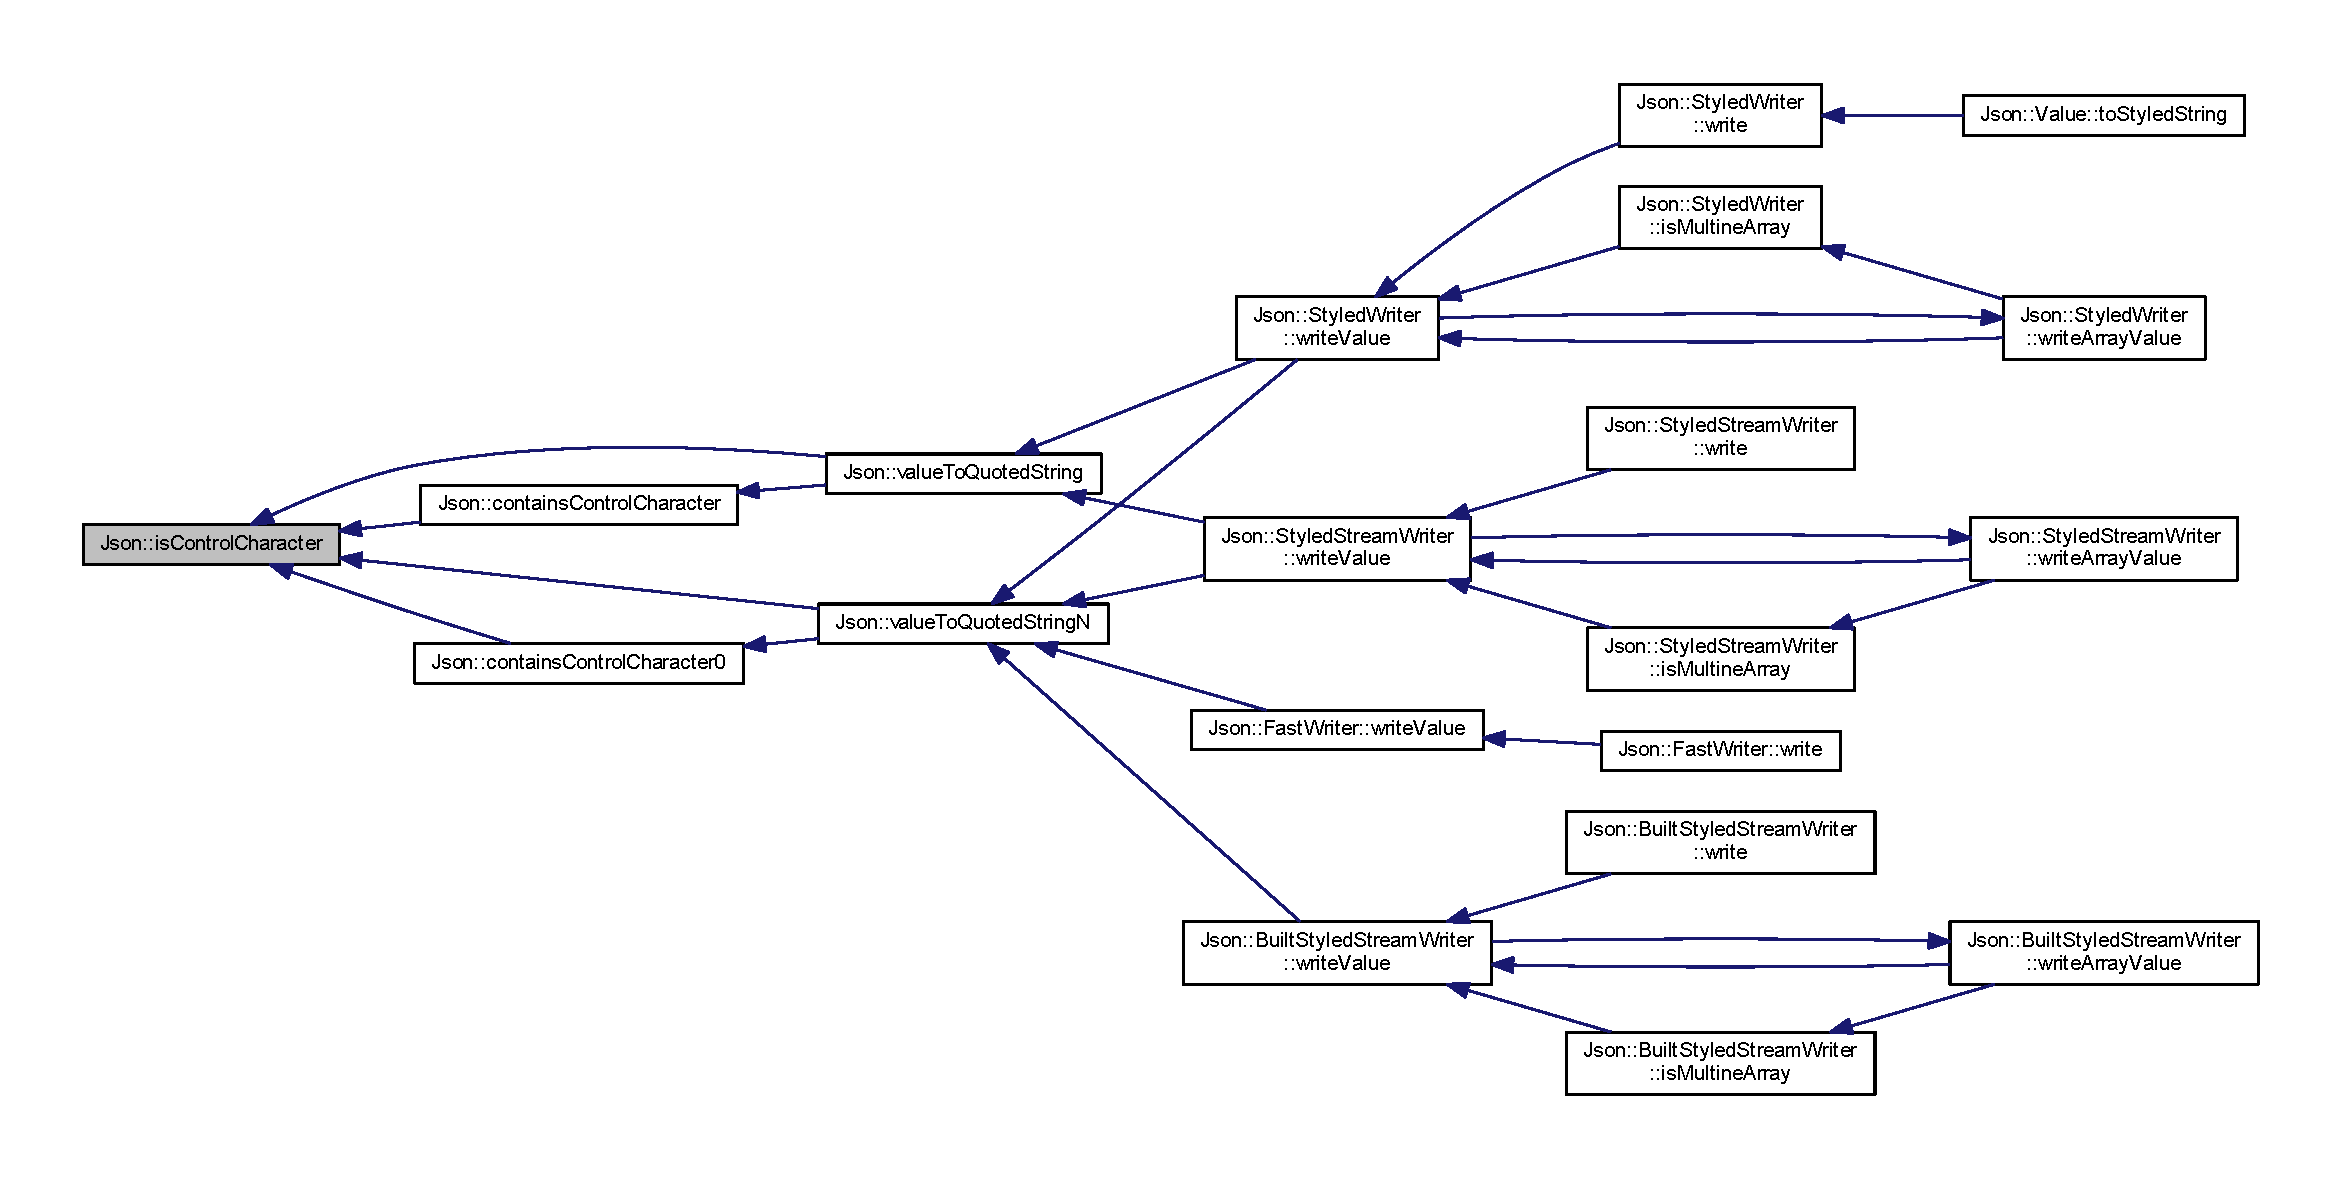
\includegraphics[width=350pt]{namespace_json_a0381e631737f51331065a388f4f59197_icgraph}
\end{center}
\end{figure}
\mbox{\Hypertarget{namespace_json_a1a04cc9d31e64b5912dade003c9b99b5}\label{namespace_json_a1a04cc9d31e64b5912dade003c9b99b5}} 
\index{Json@{Json}!Is\+Integral@{Is\+Integral}}
\index{Is\+Integral@{Is\+Integral}!Json@{Json}}
\subsubsection{\texorpdfstring{Is\+Integral()}{IsIntegral()}}
{\footnotesize\ttfamily static bool Json\+::\+Is\+Integral (\begin{DoxyParamCaption}\item[{double}]{d }\end{DoxyParamCaption})\hspace{0.3cm}{\ttfamily [static]}}



jsoncpp.\+cpp 파일의 3719 번째 라인에서 정의되었습니다.


\begin{DoxyCode}
3719                                  \{
3720   \textcolor{keywordtype}{double} integral\_part;
3721   \textcolor{keywordflow}{return} modf(d, &integral\_part) == 0.0;
3722 \}
\end{DoxyCode}
이 함수를 호출하는 함수들에 대한 그래프입니다.\+:\nopagebreak
\begin{figure}[H]
\begin{center}
\leavevmode
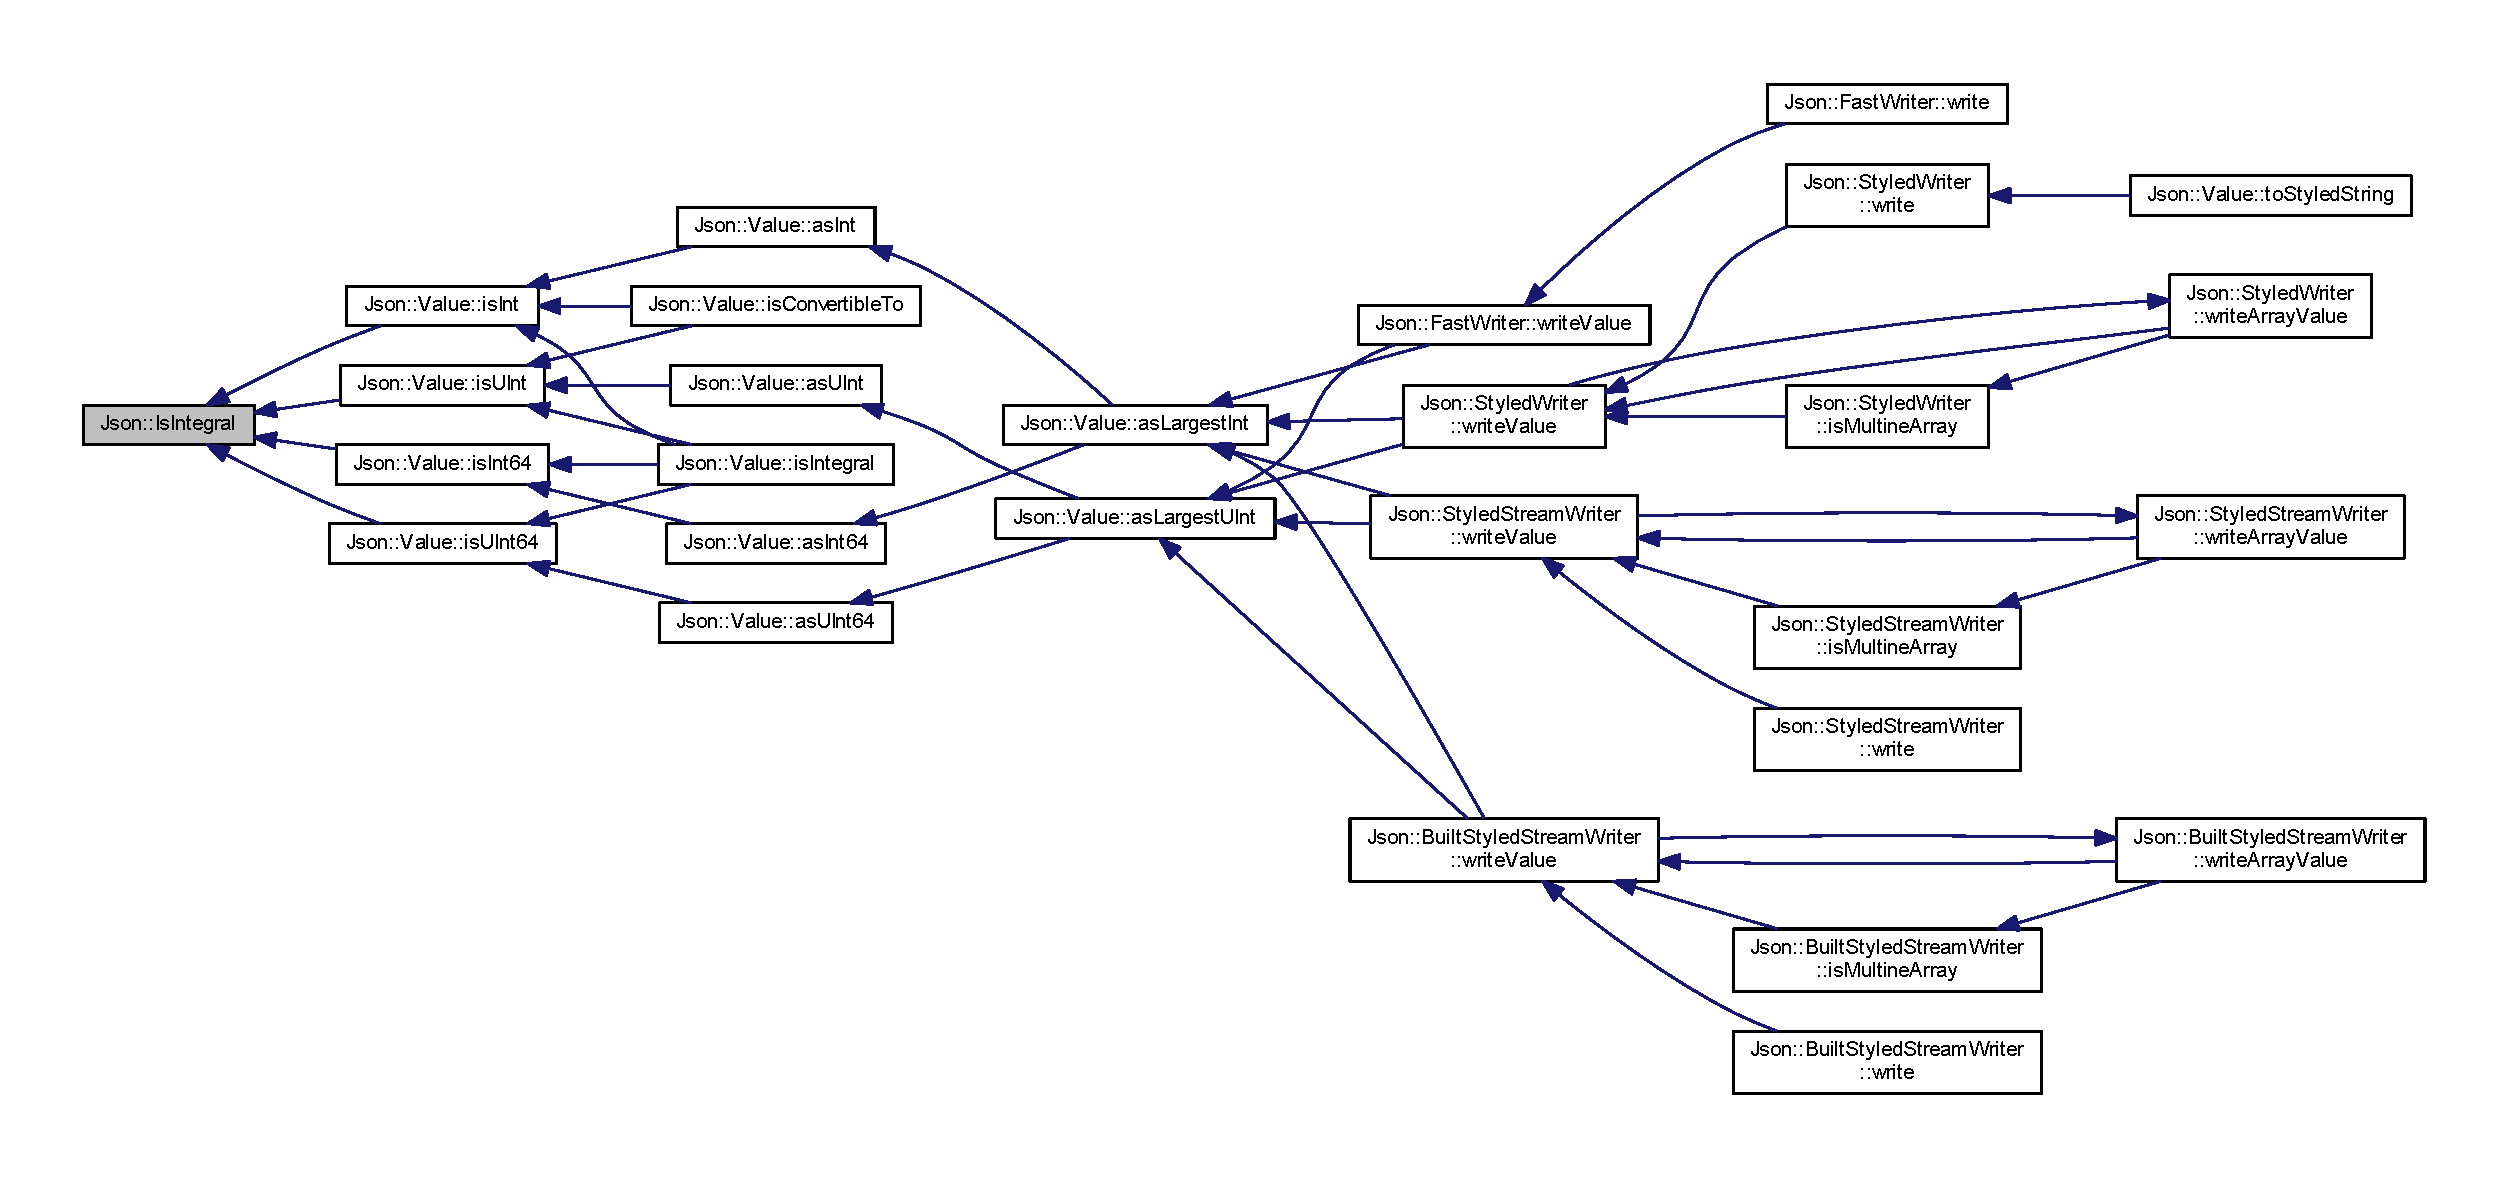
\includegraphics[width=350pt]{namespace_json_a1a04cc9d31e64b5912dade003c9b99b5_icgraph}
\end{center}
\end{figure}
\mbox{\Hypertarget{namespace_json_a63123f3dd63f340ac517a59f44ea7aa4}\label{namespace_json_a63123f3dd63f340ac517a59f44ea7aa4}} 
\index{Json@{Json}!normalize\+E\+OL@{normalize\+E\+OL}}
\index{normalize\+E\+OL@{normalize\+E\+OL}!Json@{Json}}
\subsubsection{\texorpdfstring{normalize\+E\+O\+L()}{normalizeEOL()}}
{\footnotesize\ttfamily static \hyperlink{json_8h_a1e723f95759de062585bc4a8fd3fa4be}{J\+S\+O\+N\+C\+P\+P\+\_\+\+S\+T\+R\+I\+NG} Json\+::normalize\+E\+OL (\begin{DoxyParamCaption}\item[{\hyperlink{class_json_1_1_reader_a46795b5b272bf79a7730e406cb96375a}{Reader\+::\+Location}}]{begin,  }\item[{\hyperlink{class_json_1_1_reader_a46795b5b272bf79a7730e406cb96375a}{Reader\+::\+Location}}]{end }\end{DoxyParamCaption})\hspace{0.3cm}{\ttfamily [static]}}



jsoncpp.\+cpp 파일의 590 번째 라인에서 정의되었습니다.


\begin{DoxyCode}
590                                                                              \{
591   \hyperlink{json-forwards_8h_a1e723f95759de062585bc4a8fd3fa4be}{JSONCPP\_STRING} normalized;
592   normalized.reserve(static\_cast<size\_t>(end - begin));
593   \hyperlink{class_json_1_1_reader_a46795b5b272bf79a7730e406cb96375a}{Reader::Location} current = begin;
594   \textcolor{keywordflow}{while} (current != end) \{
595     \textcolor{keywordtype}{char} c = *current++;
596     \textcolor{keywordflow}{if} (c == \textcolor{charliteral}{'\(\backslash\)r'}) \{
597       \textcolor{keywordflow}{if} (current != end && *current == \textcolor{charliteral}{'\(\backslash\)n'})
598          \textcolor{comment}{// convert dos EOL}
599          ++current;
600       \textcolor{comment}{// convert Mac EOL}
601       normalized += \textcolor{charliteral}{'\(\backslash\)n'};
602     \} \textcolor{keywordflow}{else} \{
603       normalized += c;
604     \}
605   \}
606   \textcolor{keywordflow}{return} normalized;
607 \}
\end{DoxyCode}
이 함수를 호출하는 함수들에 대한 그래프입니다.\+:\nopagebreak
\begin{figure}[H]
\begin{center}
\leavevmode
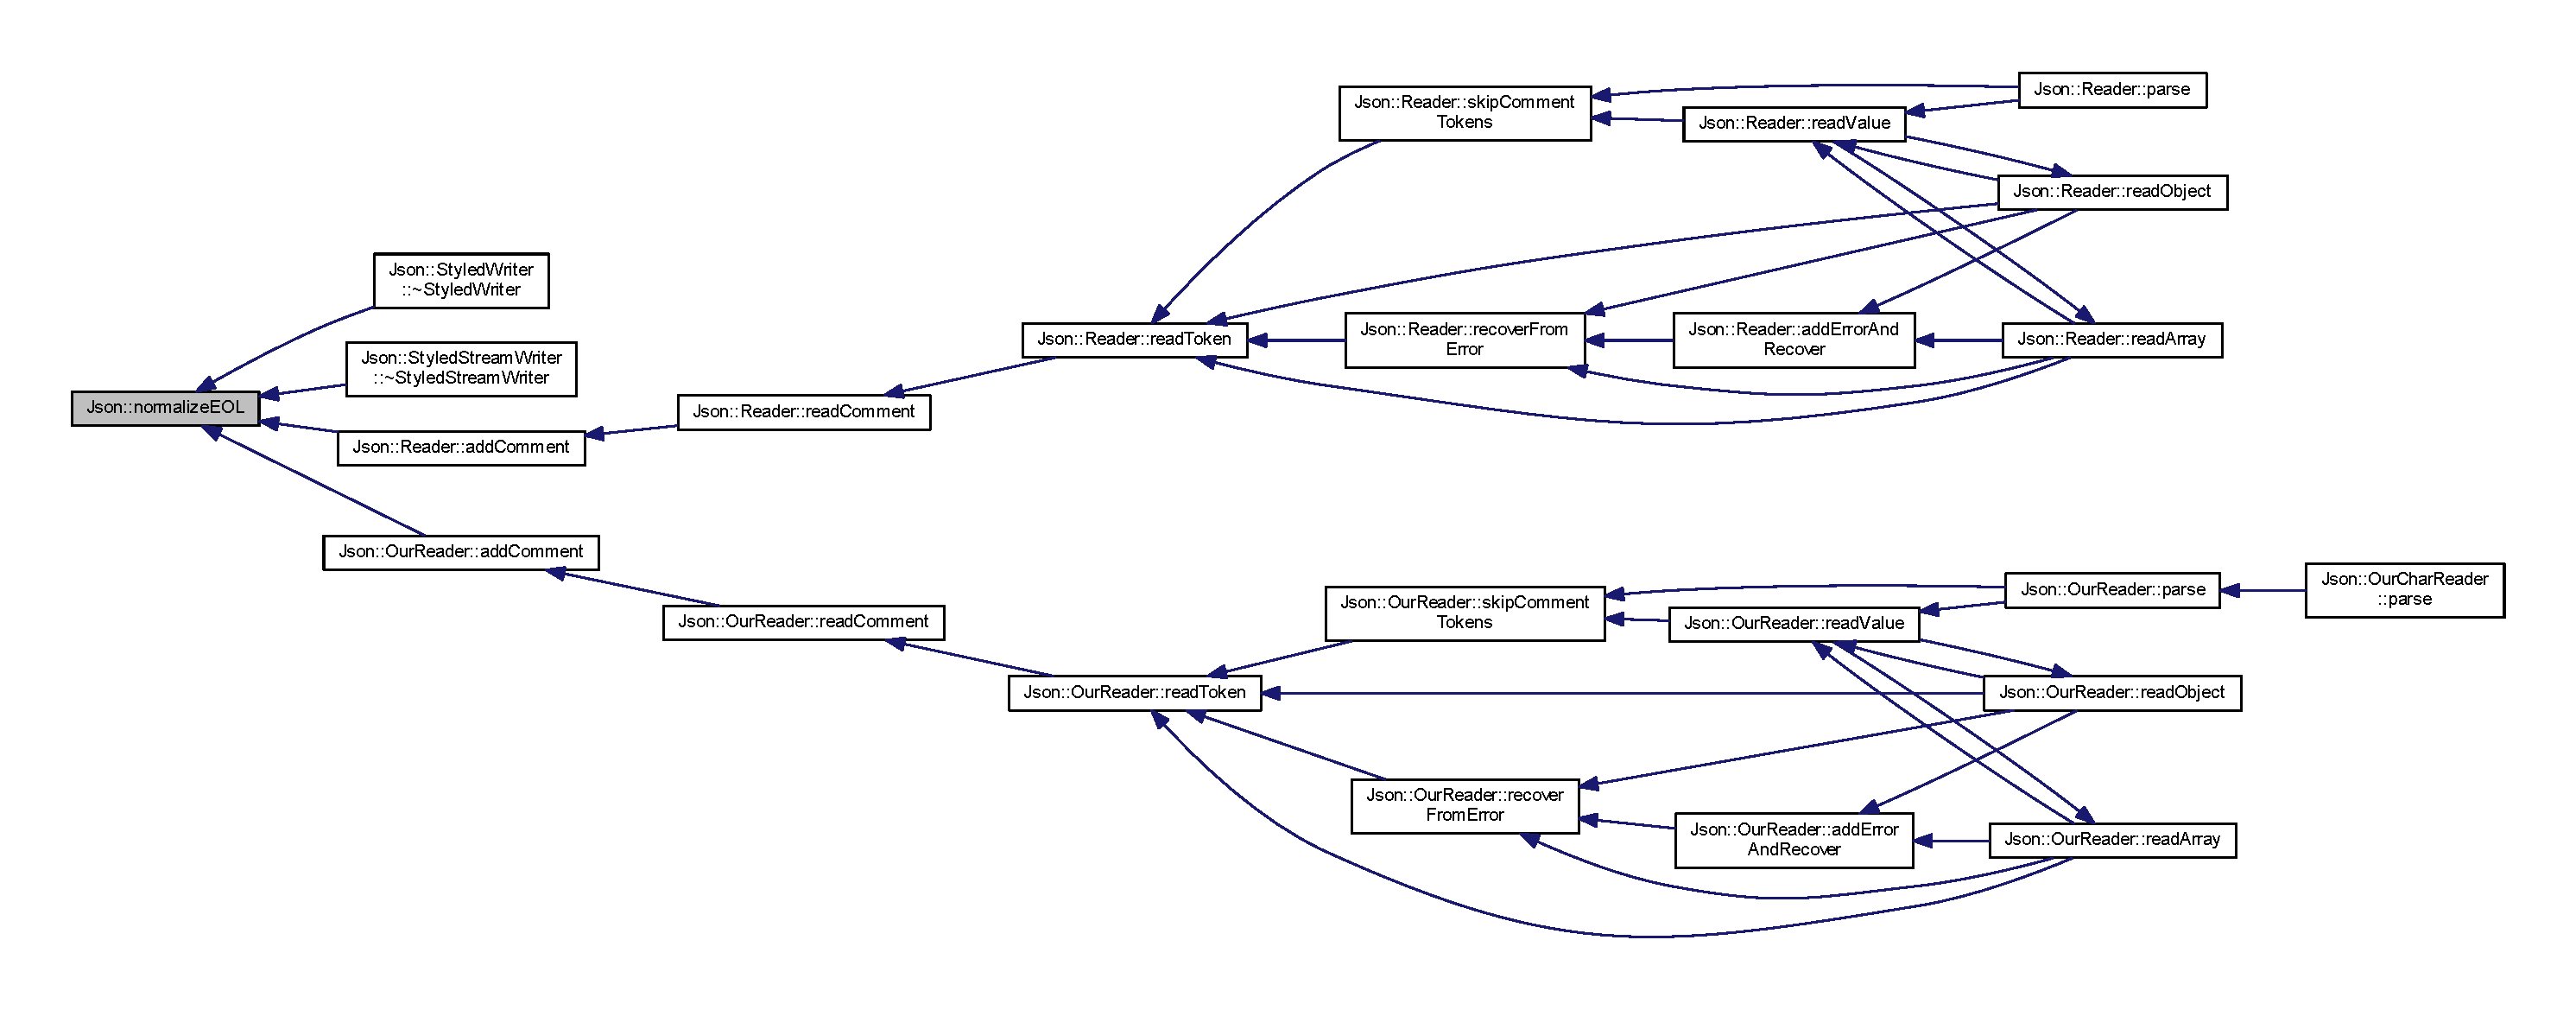
\includegraphics[width=350pt]{namespace_json_a63123f3dd63f340ac517a59f44ea7aa4_icgraph}
\end{center}
\end{figure}
\mbox{\Hypertarget{namespace_json_a975d1dbca8aa7a06f38d373edcb9081c}\label{namespace_json_a975d1dbca8aa7a06f38d373edcb9081c}} 
\index{Json@{Json}!operator$<$$<$@{operator$<$$<$}}
\index{operator$<$$<$@{operator$<$$<$}!Json@{Json}}
\subsubsection{\texorpdfstring{operator$<$$<$()}{operator<<()}}
{\footnotesize\ttfamily \hyperlink{json_8h_a37a25be5fca174927780caeb280094ce}{J\+S\+O\+N\+C\+P\+P\+\_\+\+O\+S\+T\+R\+E\+AM} \& Json\+::operator$<$$<$ (\begin{DoxyParamCaption}\item[{\hyperlink{json_8h_a37a25be5fca174927780caeb280094ce}{J\+S\+O\+N\+C\+P\+P\+\_\+\+O\+S\+T\+R\+E\+AM} \&}]{sout,  }\item[{const \hyperlink{class_json_1_1_value}{Value} \&}]{root }\end{DoxyParamCaption})}



Output using the \hyperlink{class_json_1_1_styled_stream_writer}{Styled\+Stream\+Writer}. 

\begin{DoxySeeAlso}{참고}
\hyperlink{namespace_json_a244ed0996aba750c40c1641c06bba449}{Json\+::operator$>$$>$()} 
\end{DoxySeeAlso}


jsoncpp.\+cpp 파일의 5296 번째 라인에서 정의되었습니다.


\begin{DoxyCode}
5296                                                                       \{
5297   \hyperlink{class_json_1_1_stream_writer_builder}{StreamWriterBuilder} builder;
5298   \hyperlink{namespace_json_a7132404aeebfc96d7c6ad2c66260afb5}{StreamWriterPtr} \textcolor{keyword}{const} writer(builder.\hyperlink{class_json_1_1_stream_writer_builder_ab9ee278609f88ae04a7c1a84e1f559e6}{newStreamWriter}());
5299   writer->write(root, &sout);
5300   \textcolor{keywordflow}{return} sout;
5301 \}
\end{DoxyCode}
이 함수 내부에서 호출하는 함수들에 대한 그래프입니다.\+:\nopagebreak
\begin{figure}[H]
\begin{center}
\leavevmode
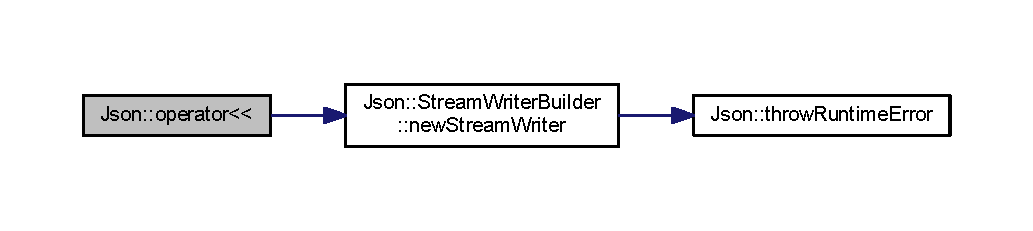
\includegraphics[width=350pt]{namespace_json_a975d1dbca8aa7a06f38d373edcb9081c_cgraph}
\end{center}
\end{figure}
\mbox{\Hypertarget{namespace_json_a244ed0996aba750c40c1641c06bba449}\label{namespace_json_a244ed0996aba750c40c1641c06bba449}} 
\index{Json@{Json}!operator$>$$>$@{operator$>$$>$}}
\index{operator$>$$>$@{operator$>$$>$}!Json@{Json}}
\subsubsection{\texorpdfstring{operator$>$$>$()}{operator>>()}}
{\footnotesize\ttfamily \hyperlink{json_8h_a15f2f70b2ce0a2abd0f8112393dbc4de}{J\+S\+O\+N\+C\+P\+P\+\_\+\+I\+S\+T\+R\+E\+AM} \& Json\+::operator$>$$>$ (\begin{DoxyParamCaption}\item[{\hyperlink{json_8h_a15f2f70b2ce0a2abd0f8112393dbc4de}{J\+S\+O\+N\+C\+P\+P\+\_\+\+I\+S\+T\+R\+E\+AM} \&}]{sin,  }\item[{\hyperlink{class_json_1_1_value}{Value} \&}]{root }\end{DoxyParamCaption})}



Read from \textquotesingle{}sin\textquotesingle{} into \textquotesingle{}root\textquotesingle{}. 

Always keep comments from the input J\+S\+ON.

This can be used to read a file into a particular sub-\/object. For example\+: 
\begin{DoxyCode}
\hyperlink{class_json_1_1_value}{Json::Value} root;
cin >> root[\textcolor{stringliteral}{"dir"}][\textcolor{stringliteral}{"file"}];
cout << root;
\end{DoxyCode}
 Result\+: \begin{DoxyVerb}{
"dir": {
    "file": {
    // The input stream JSON would be nested here.
    }
}
}
\end{DoxyVerb}
 
\begin{DoxyExceptions}{예외}
{\em std\+::exception} & on parse error. \\
\hline
\end{DoxyExceptions}
\begin{DoxySeeAlso}{참고}
\hyperlink{namespace_json_a975d1dbca8aa7a06f38d373edcb9081c}{Json\+::operator$<$$<$()} 
\end{DoxySeeAlso}


jsoncpp.\+cpp 파일의 2239 번째 라인에서 정의되었습니다.


\begin{DoxyCode}
2239                                                                \{
2240   \hyperlink{class_json_1_1_char_reader_builder}{CharReaderBuilder} b;
2241   \hyperlink{json-forwards_8h_a1e723f95759de062585bc4a8fd3fa4be}{JSONCPP\_STRING} errs;
2242   \textcolor{keywordtype}{bool} ok = \hyperlink{namespace_json_a38f903cfdb57a6c4e86a7dcc42f3712c}{parseFromStream}(b, sin, &root, &errs);
2243   \textcolor{keywordflow}{if} (!ok) \{
2244     fprintf(stderr,
2245             \textcolor{stringliteral}{"Error from reader: %s"},
2246             errs.c\_str());
2247 
2248     \hyperlink{namespace_json_a0ab7ff7f99788262d92d9ff3d924e065}{throwRuntimeError}(errs);
2249   \}
2250   \textcolor{keywordflow}{return} sin;
2251 \}
\end{DoxyCode}
이 함수 내부에서 호출하는 함수들에 대한 그래프입니다.\+:\nopagebreak
\begin{figure}[H]
\begin{center}
\leavevmode
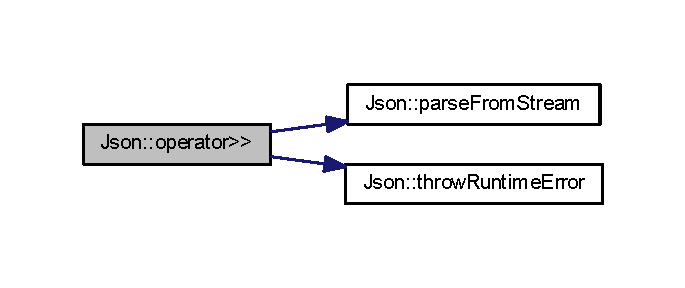
\includegraphics[width=329pt]{namespace_json_a244ed0996aba750c40c1641c06bba449_cgraph}
\end{center}
\end{figure}
\mbox{\Hypertarget{namespace_json_aab0cf1ecf81d1aeca12be2a416a84352}\label{namespace_json_aab0cf1ecf81d1aeca12be2a416a84352}} 
\index{Json@{Json}!parse\+From\+Stream@{parse\+From\+Stream}}
\index{parse\+From\+Stream@{parse\+From\+Stream}!Json@{Json}}
\subsubsection{\texorpdfstring{parse\+From\+Stream()}{parseFromStream()}\hspace{0.1cm}{\footnotesize\ttfamily [1/2]}}
{\footnotesize\ttfamily bool \hyperlink{json_8h_a1d61ffde86ce1a18fd83194ff0d9a206}{J\+S\+O\+N\+\_\+\+A\+PI} Json\+::parse\+From\+Stream (\begin{DoxyParamCaption}\item[{\hyperlink{class_json_1_1_char_reader_1_1_factory}{Char\+Reader\+::\+Factory} const \&}]{,  }\item[{\hyperlink{json_8h_a15f2f70b2ce0a2abd0f8112393dbc4de}{J\+S\+O\+N\+C\+P\+P\+\_\+\+I\+S\+T\+R\+E\+AM} \&}]{,  }\item[{\hyperlink{class_json_1_1_value}{Value} $\ast$}]{root,  }\item[{std\+::string $\ast$}]{errs }\end{DoxyParamCaption})}

Consume entire stream and use its begin/end. Someday we might have a real Stream\+Reader, but for now this is convenient. 이 함수를 호출하는 함수들에 대한 그래프입니다.\+:\nopagebreak
\begin{figure}[H]
\begin{center}
\leavevmode
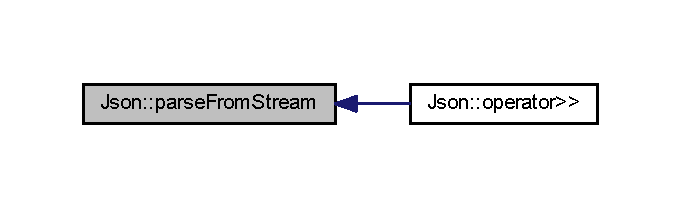
\includegraphics[width=327pt]{namespace_json_aab0cf1ecf81d1aeca12be2a416a84352_icgraph}
\end{center}
\end{figure}
\mbox{\Hypertarget{namespace_json_a38f903cfdb57a6c4e86a7dcc42f3712c}\label{namespace_json_a38f903cfdb57a6c4e86a7dcc42f3712c}} 
\index{Json@{Json}!parse\+From\+Stream@{parse\+From\+Stream}}
\index{parse\+From\+Stream@{parse\+From\+Stream}!Json@{Json}}
\subsubsection{\texorpdfstring{parse\+From\+Stream()}{parseFromStream()}\hspace{0.1cm}{\footnotesize\ttfamily [2/2]}}
{\footnotesize\ttfamily bool Json\+::parse\+From\+Stream (\begin{DoxyParamCaption}\item[{\hyperlink{class_json_1_1_char_reader_1_1_factory}{Char\+Reader\+::\+Factory} const \&}]{fact,  }\item[{\hyperlink{json_8h_a15f2f70b2ce0a2abd0f8112393dbc4de}{J\+S\+O\+N\+C\+P\+P\+\_\+\+I\+S\+T\+R\+E\+AM} \&}]{sin,  }\item[{\hyperlink{class_json_1_1_value}{Value} $\ast$}]{root,  }\item[{\hyperlink{json_8h_a1e723f95759de062585bc4a8fd3fa4be}{J\+S\+O\+N\+C\+P\+P\+\_\+\+S\+T\+R\+I\+NG} $\ast$}]{errs }\end{DoxyParamCaption})}



jsoncpp.\+cpp 파일의 2225 번째 라인에서 정의되었습니다.


\begin{DoxyCode}
2228 \{
2229   \hyperlink{json-forwards_8h_a1d06ac2ca63c8c521f41231dfda0e6b3}{JSONCPP\_OSTRINGSTREAM} ssin;
2230   ssin << sin.rdbuf();
2231   \hyperlink{json-forwards_8h_a1e723f95759de062585bc4a8fd3fa4be}{JSONCPP\_STRING} doc = ssin.str();
2232   \textcolor{keywordtype}{char} \textcolor{keyword}{const}* begin = doc.data();
2233   \textcolor{keywordtype}{char} \textcolor{keyword}{const}* end = begin + doc.size();
2234   \textcolor{comment}{// Note that we do not actually need a null-terminator.}
2235   \hyperlink{namespace_json_a4724efb8d41614b47036cb8b54233837}{CharReaderPtr} \textcolor{keyword}{const} reader(fact.newCharReader());
2236   \textcolor{keywordflow}{return} reader->parse(begin, end, root, errs);
2237 \}
\end{DoxyCode}
이 함수 내부에서 호출하는 함수들에 대한 그래프입니다.\+:\nopagebreak
\begin{figure}[H]
\begin{center}
\leavevmode
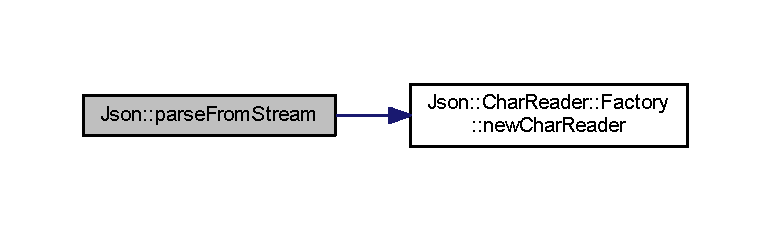
\includegraphics[width=350pt]{namespace_json_a38f903cfdb57a6c4e86a7dcc42f3712c_cgraph}
\end{center}
\end{figure}
\mbox{\Hypertarget{namespace_json_a48f4e3ea655e3b4a5d7f892c81f00511}\label{namespace_json_a48f4e3ea655e3b4a5d7f892c81f00511}} 
\index{Json@{Json}!release\+Prefixed\+String\+Value@{release\+Prefixed\+String\+Value}}
\index{release\+Prefixed\+String\+Value@{release\+Prefixed\+String\+Value}!Json@{Json}}
\subsubsection{\texorpdfstring{release\+Prefixed\+String\+Value()}{releasePrefixedStringValue()}}
{\footnotesize\ttfamily static void Json\+::release\+Prefixed\+String\+Value (\begin{DoxyParamCaption}\item[{char $\ast$}]{value }\end{DoxyParamCaption})\hspace{0.3cm}{\ttfamily [inline]}, {\ttfamily [static]}}

Free the string duplicated by \hyperlink{namespace_json_a678ac3a60cd70ec0fb4c9abfd40eb0c4}{duplicate\+String\+Value()}/duplicate\+And\+Prefix\+String\+Value(). 

jsoncpp.\+cpp 파일의 2617 번째 라인에서 정의되었습니다.


\begin{DoxyCode}
2617                                                            \{
2618   free(value);
2619 \}
\end{DoxyCode}
이 함수를 호출하는 함수들에 대한 그래프입니다.\+:\nopagebreak
\begin{figure}[H]
\begin{center}
\leavevmode
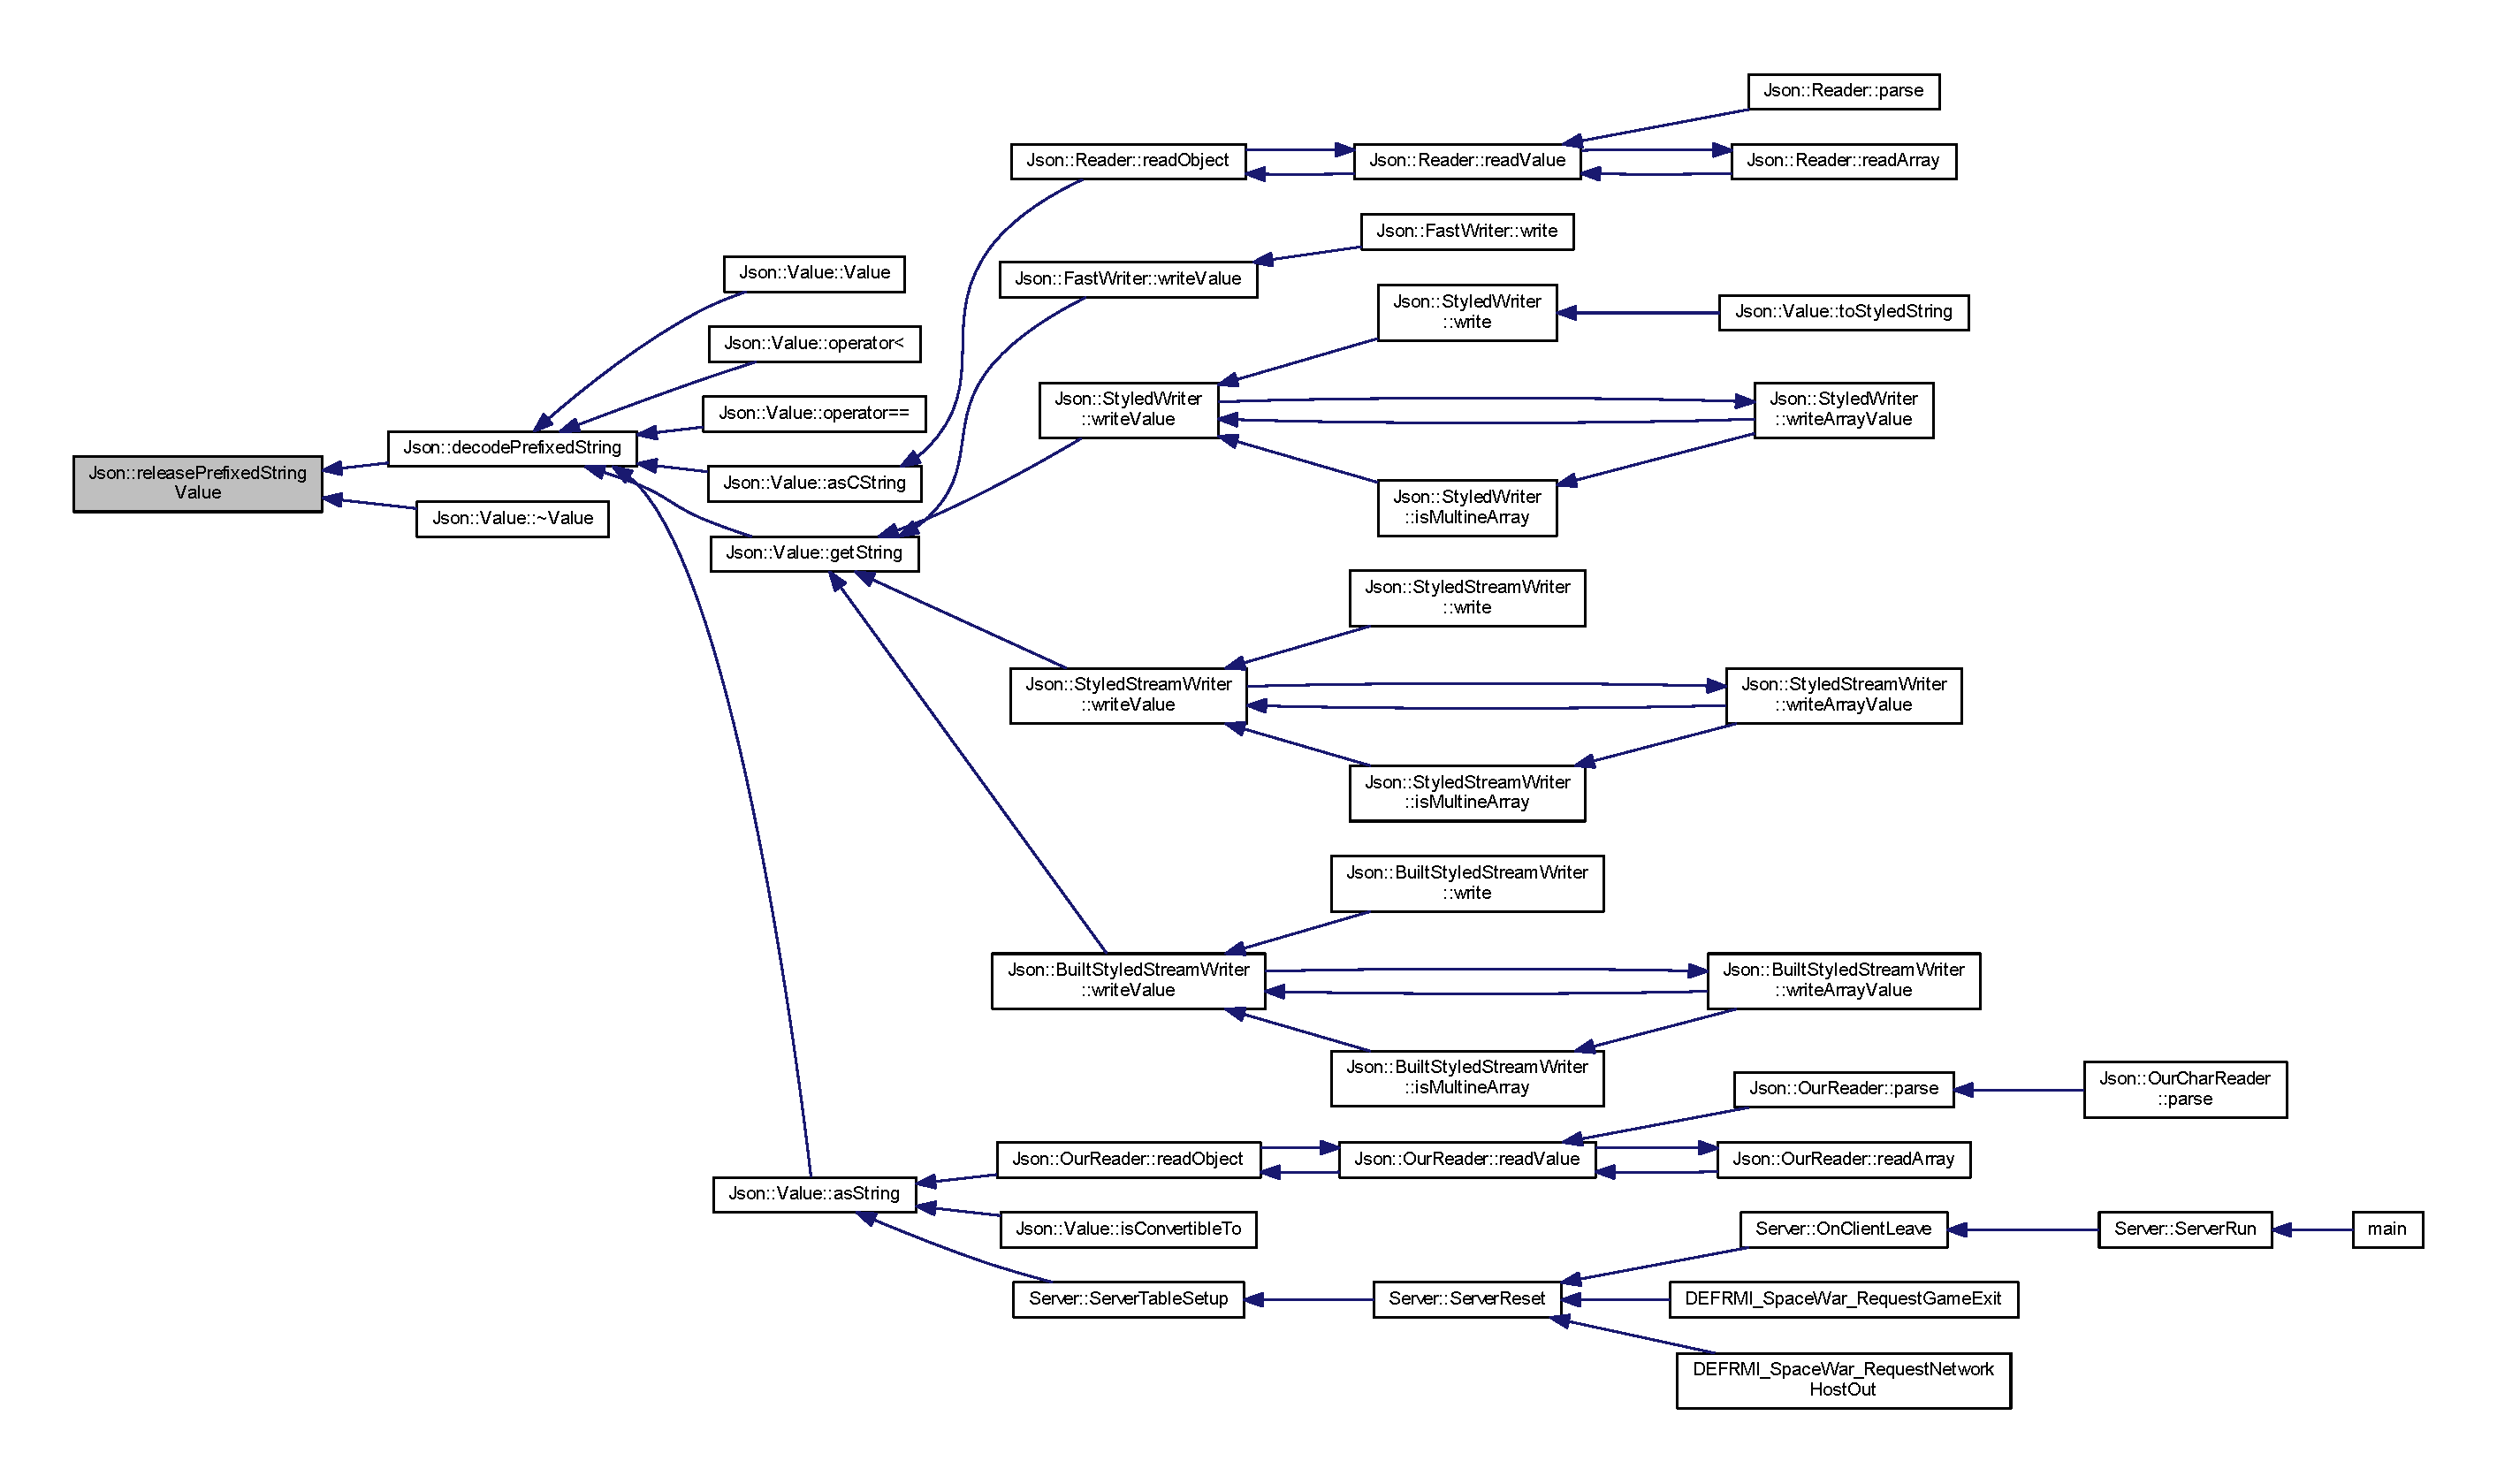
\includegraphics[width=350pt]{namespace_json_a48f4e3ea655e3b4a5d7f892c81f00511_icgraph}
\end{center}
\end{figure}
\mbox{\Hypertarget{namespace_json_a3e0d81d514d0e8bddf33b08074214abd}\label{namespace_json_a3e0d81d514d0e8bddf33b08074214abd}} 
\index{Json@{Json}!release\+String\+Value@{release\+String\+Value}}
\index{release\+String\+Value@{release\+String\+Value}!Json@{Json}}
\subsubsection{\texorpdfstring{release\+String\+Value()}{releaseStringValue()}}
{\footnotesize\ttfamily static void Json\+::release\+String\+Value (\begin{DoxyParamCaption}\item[{char $\ast$}]{value,  }\item[{unsigned}]{ }\end{DoxyParamCaption})\hspace{0.3cm}{\ttfamily [inline]}, {\ttfamily [static]}}



jsoncpp.\+cpp 파일의 2620 번째 라인에서 정의되었습니다.


\begin{DoxyCode}
2620                                                              \{
2621   free(value);
2622 \}
\end{DoxyCode}
이 함수를 호출하는 함수들에 대한 그래프입니다.\+:
\nopagebreak
\begin{figure}[H]
\begin{center}
\leavevmode
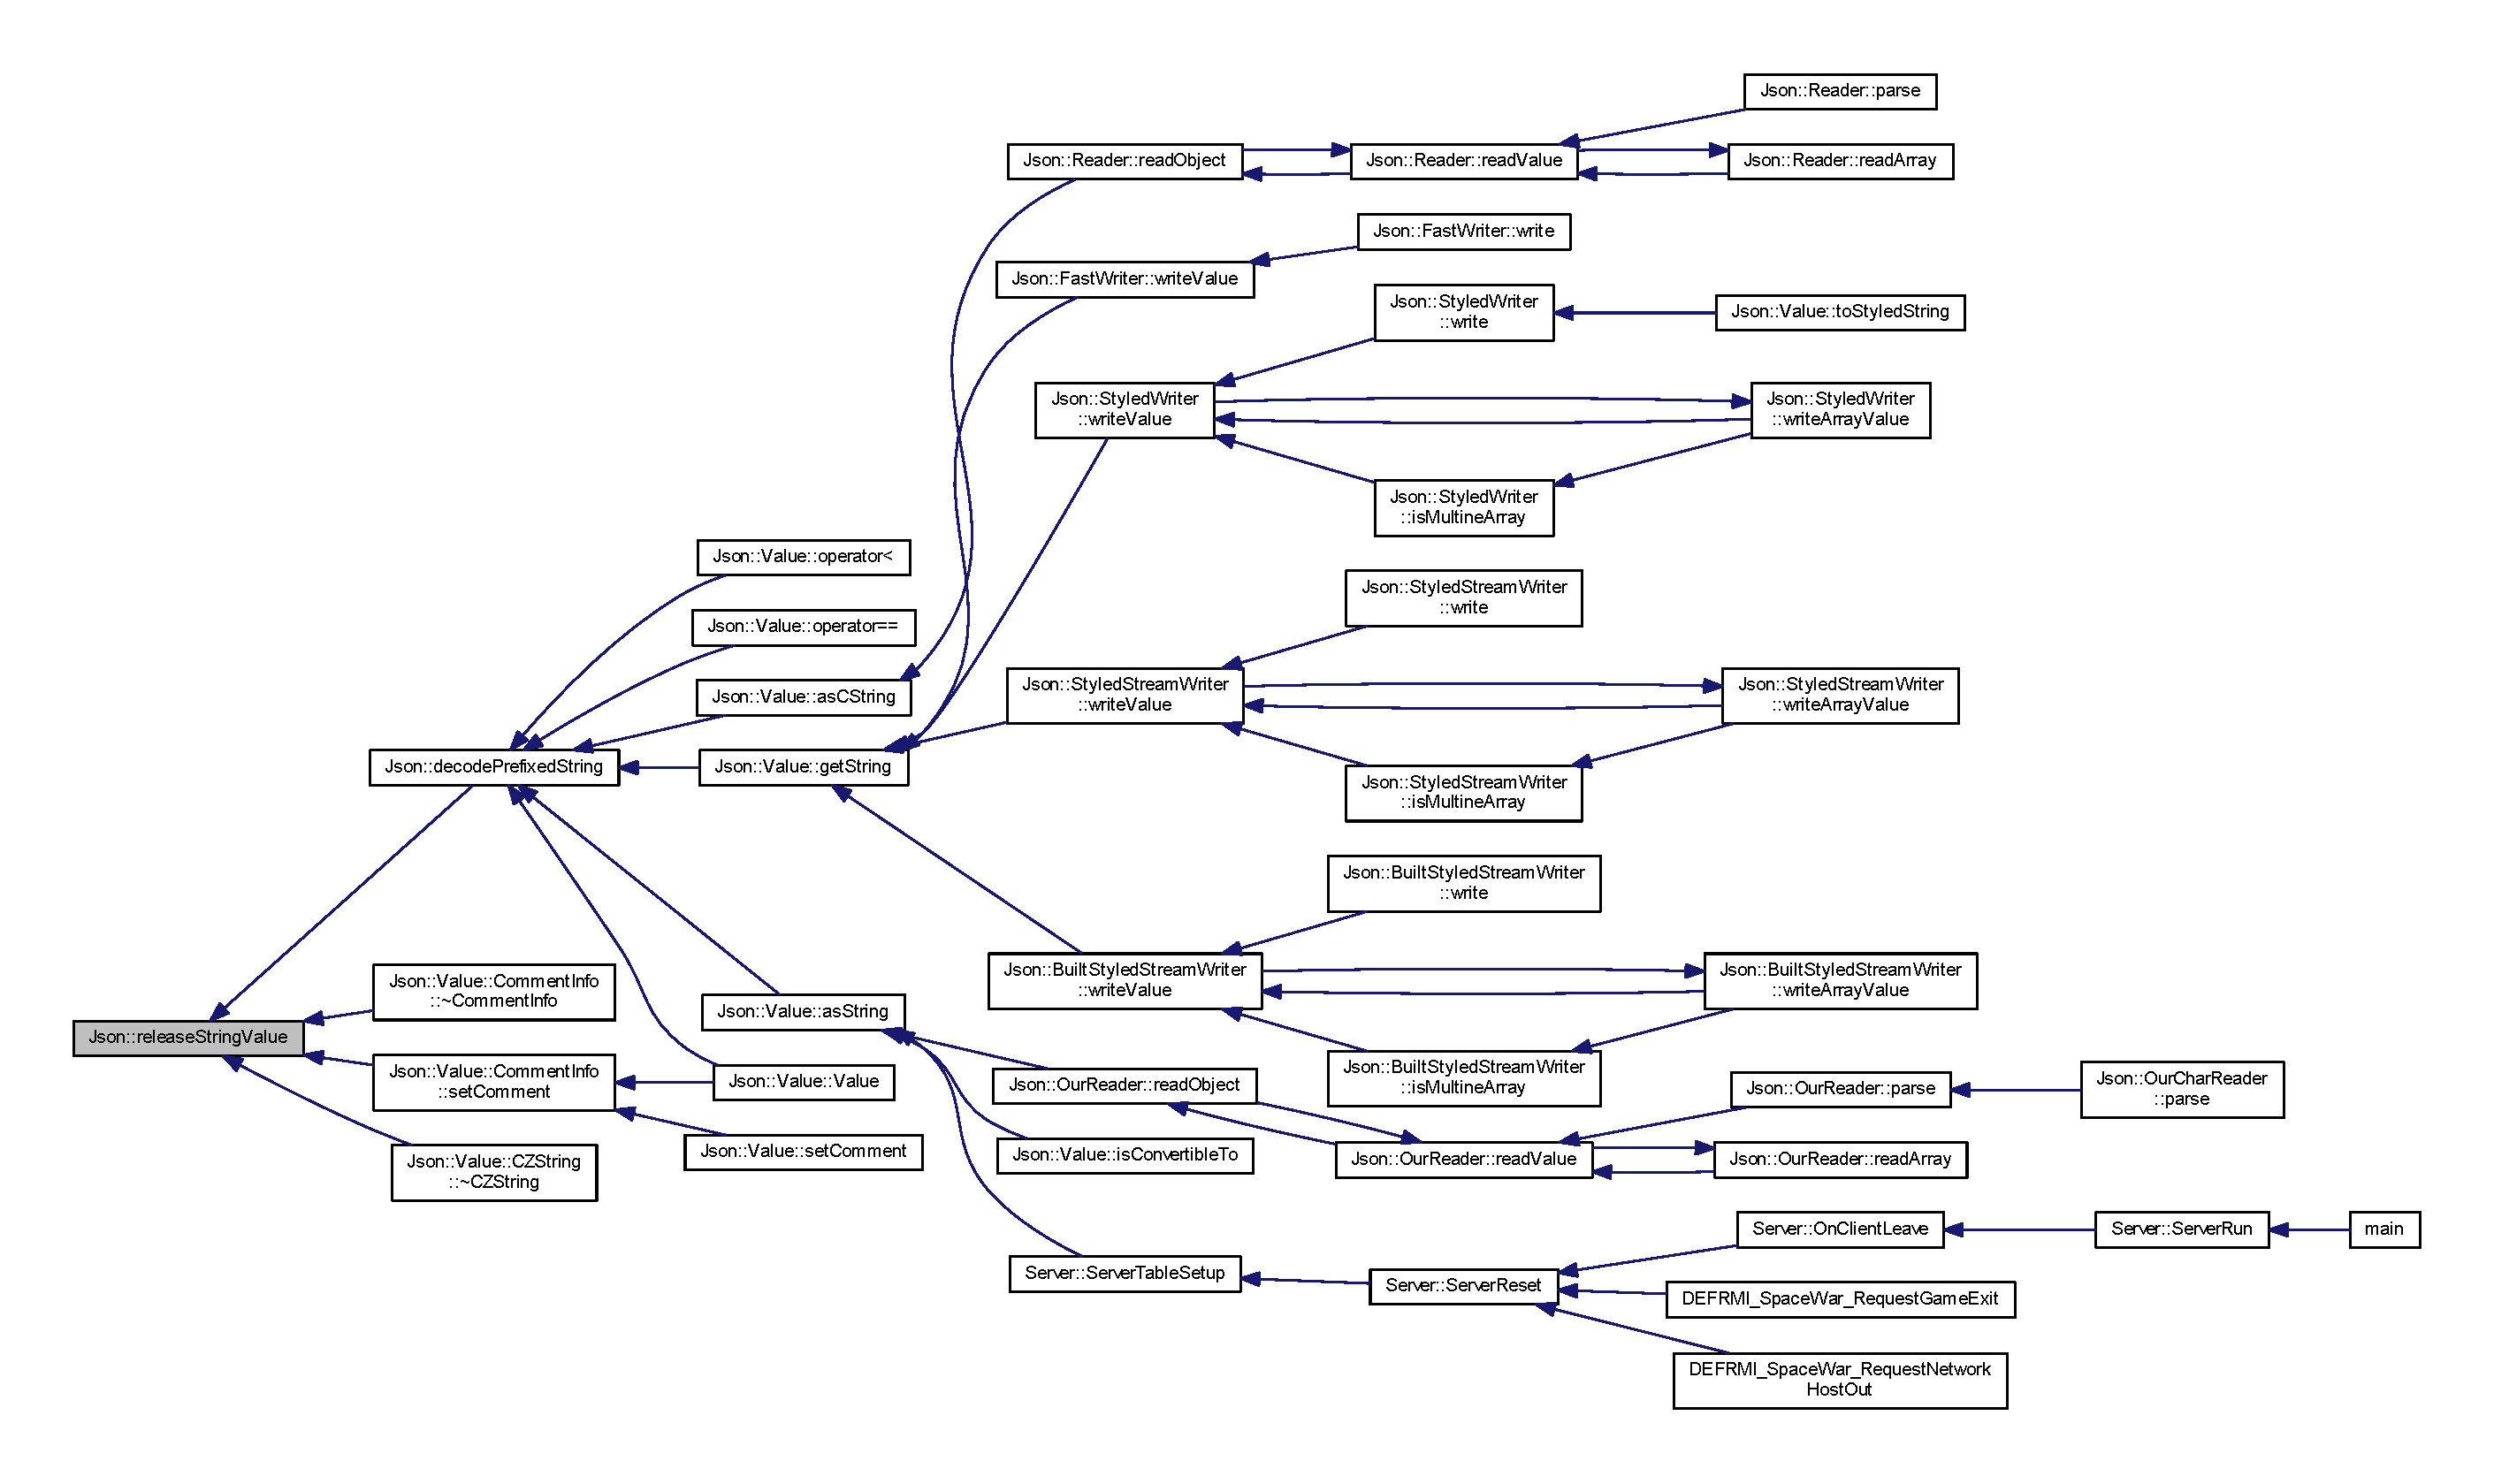
\includegraphics[width=350pt]{namespace_json_a3e0d81d514d0e8bddf33b08074214abd_icgraph}
\end{center}
\end{figure}
\mbox{\Hypertarget{namespace_json_a7492156d0c7d2dd2f672acacfb240320}\label{namespace_json_a7492156d0c7d2dd2f672acacfb240320}} 
\index{Json@{Json}!strnpbrk@{strnpbrk}}
\index{strnpbrk@{strnpbrk}!Json@{Json}}
\subsubsection{\texorpdfstring{strnpbrk()}{strnpbrk()}}
{\footnotesize\ttfamily static char const$\ast$ Json\+::strnpbrk (\begin{DoxyParamCaption}\item[{char const $\ast$}]{s,  }\item[{char const $\ast$}]{accept,  }\item[{size\+\_\+t}]{n }\end{DoxyParamCaption})\hspace{0.3cm}{\ttfamily [static]}}



jsoncpp.\+cpp 파일의 4322 번째 라인에서 정의되었습니다.


\begin{DoxyCode}
4322                                                                          \{
4323   assert((s || !n) && accept);
4324 
4325   \textcolor{keywordtype}{char} \textcolor{keyword}{const}* \textcolor{keyword}{const} end = s + n;
4326   \textcolor{keywordflow}{for} (\textcolor{keywordtype}{char} \textcolor{keyword}{const}* cur = s; cur < end; ++cur) \{
4327     \textcolor{keywordtype}{int} \textcolor{keyword}{const} c = *cur;
4328     \textcolor{keywordflow}{for} (\textcolor{keywordtype}{char} \textcolor{keyword}{const}* a = accept; *a; ++a) \{
4329       \textcolor{keywordflow}{if} (*a == c) \{
4330         \textcolor{keywordflow}{return} cur;
4331       \}
4332     \}
4333   \}
4334   \textcolor{keywordflow}{return} NULL;
4335 \}
\end{DoxyCode}
이 함수를 호출하는 함수들에 대한 그래프입니다.\+:\nopagebreak
\begin{figure}[H]
\begin{center}
\leavevmode
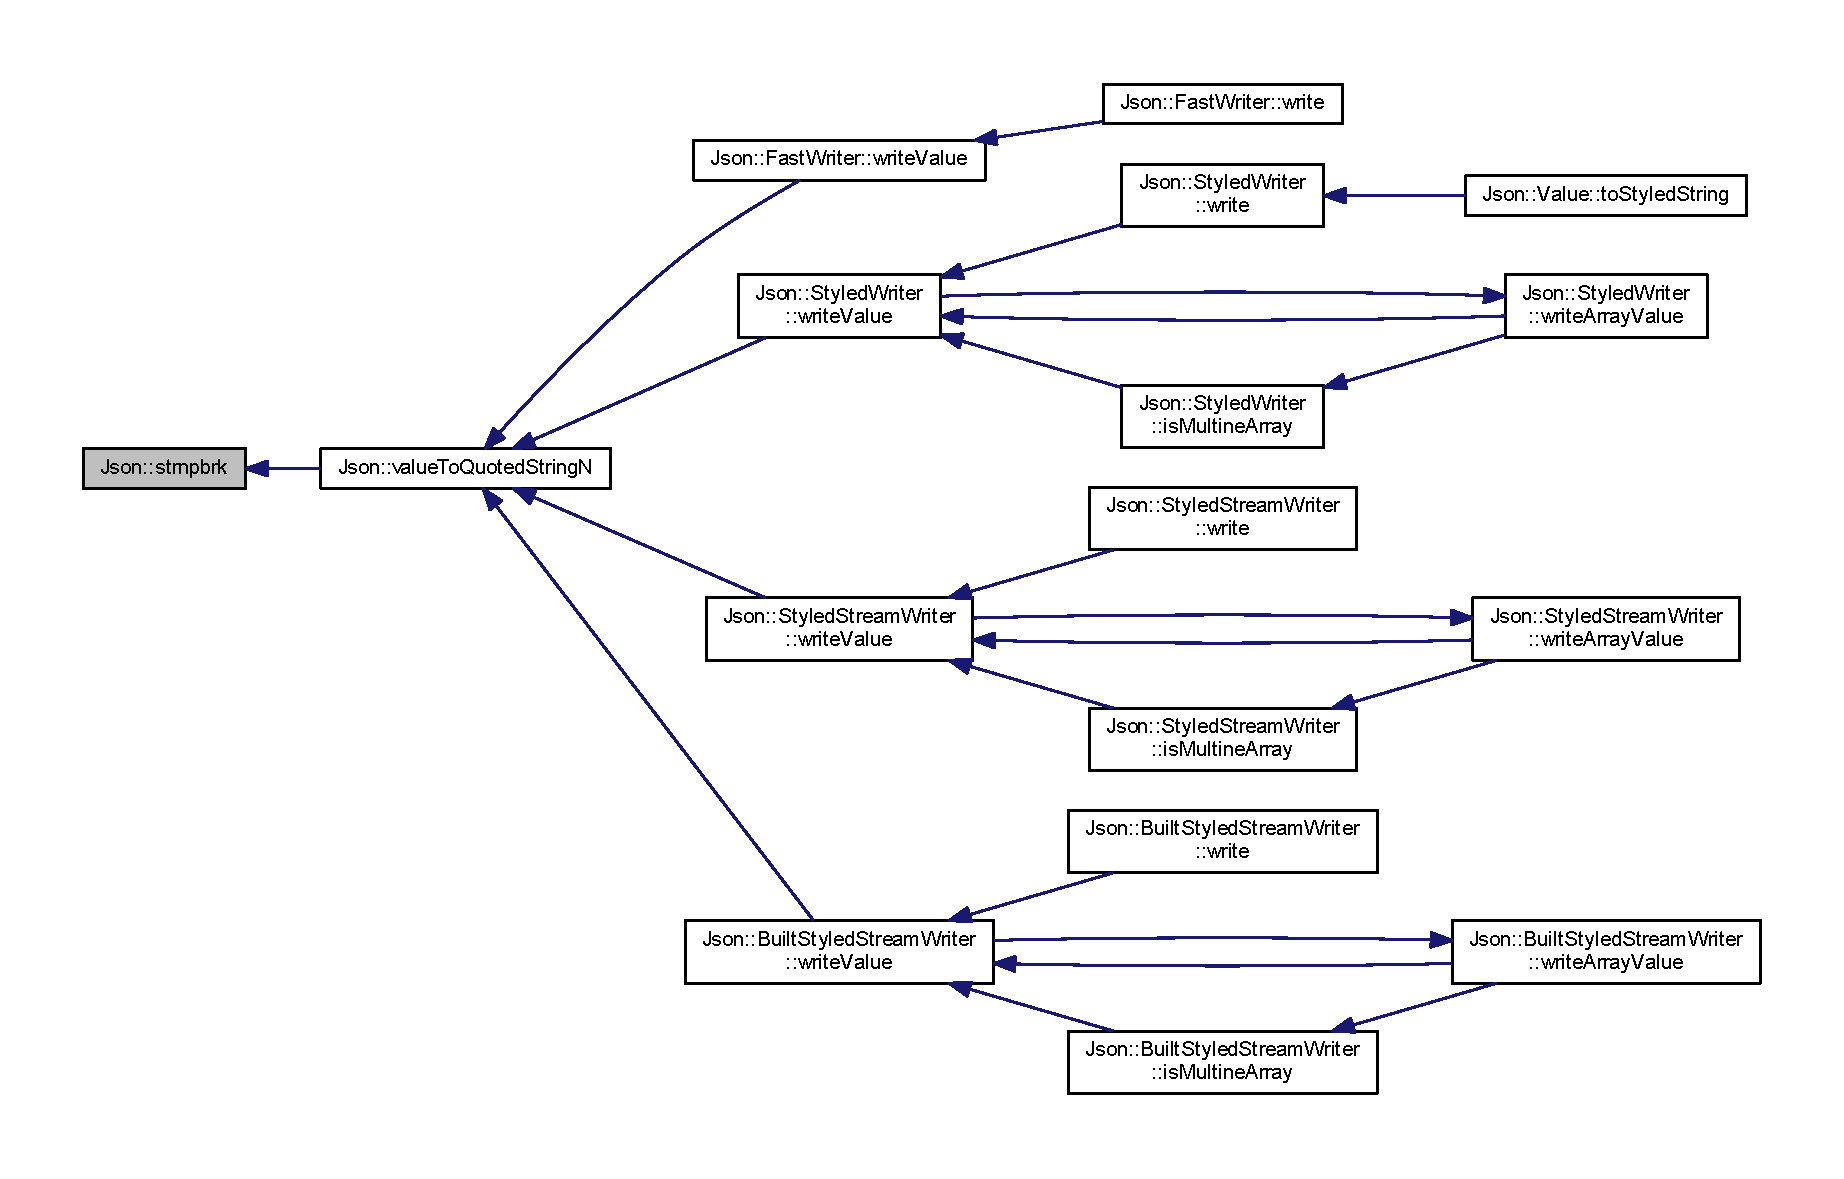
\includegraphics[width=350pt]{namespace_json_a7492156d0c7d2dd2f672acacfb240320_icgraph}
\end{center}
\end{figure}
\mbox{\Hypertarget{namespace_json_a27790f21f17922fac81e7cd72a5659a5}\label{namespace_json_a27790f21f17922fac81e7cd72a5659a5}} 
\index{Json@{Json}!throw\+Logic\+Error@{throw\+Logic\+Error}}
\index{throw\+Logic\+Error@{throw\+Logic\+Error}!Json@{Json}}
\subsubsection{\texorpdfstring{throw\+Logic\+Error()}{throwLogicError()}}
{\footnotesize\ttfamily \hyperlink{json_8h_a78c5ba441d8b48f24a5095b97f01f282}{J\+S\+O\+N\+C\+P\+P\+\_\+\+N\+O\+R\+E\+T\+U\+RN} void Json\+::throw\+Logic\+Error (\begin{DoxyParamCaption}\item[{\hyperlink{json_8h_a1e723f95759de062585bc4a8fd3fa4be}{J\+S\+O\+N\+C\+P\+P\+\_\+\+S\+T\+R\+I\+NG} const \&}]{msg }\end{DoxyParamCaption})}



used internally 



jsoncpp.\+cpp 파일의 2660 번째 라인에서 정의되었습니다.


\begin{DoxyCode}
2661 \{
2662   \textcolor{keywordflow}{throw} \hyperlink{class_json_1_1_logic_error}{LogicError}(msg);
2663 \}
\end{DoxyCode}
이 함수 내부에서 호출하는 함수들에 대한 그래프입니다.\+:\nopagebreak
\begin{figure}[H]
\begin{center}
\leavevmode
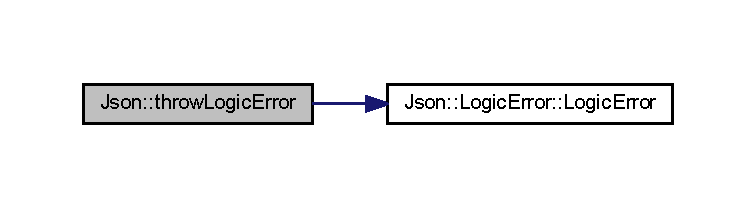
\includegraphics[width=350pt]{namespace_json_a27790f21f17922fac81e7cd72a5659a5_cgraph}
\end{center}
\end{figure}
\mbox{\Hypertarget{namespace_json_a0ab7ff7f99788262d92d9ff3d924e065}\label{namespace_json_a0ab7ff7f99788262d92d9ff3d924e065}} 
\index{Json@{Json}!throw\+Runtime\+Error@{throw\+Runtime\+Error}}
\index{throw\+Runtime\+Error@{throw\+Runtime\+Error}!Json@{Json}}
\subsubsection{\texorpdfstring{throw\+Runtime\+Error()}{throwRuntimeError()}}
{\footnotesize\ttfamily \hyperlink{json_8h_a78c5ba441d8b48f24a5095b97f01f282}{J\+S\+O\+N\+C\+P\+P\+\_\+\+N\+O\+R\+E\+T\+U\+RN} void Json\+::throw\+Runtime\+Error (\begin{DoxyParamCaption}\item[{\hyperlink{json_8h_a1e723f95759de062585bc4a8fd3fa4be}{J\+S\+O\+N\+C\+P\+P\+\_\+\+S\+T\+R\+I\+NG} const \&}]{msg }\end{DoxyParamCaption})}



used internally 



jsoncpp.\+cpp 파일의 2656 번째 라인에서 정의되었습니다.


\begin{DoxyCode}
2657 \{
2658   \textcolor{keywordflow}{throw} \hyperlink{class_json_1_1_runtime_error}{RuntimeError}(msg);
2659 \}
\end{DoxyCode}
이 함수를 호출하는 함수들에 대한 그래프입니다.\+:
\nopagebreak
\begin{figure}[H]
\begin{center}
\leavevmode
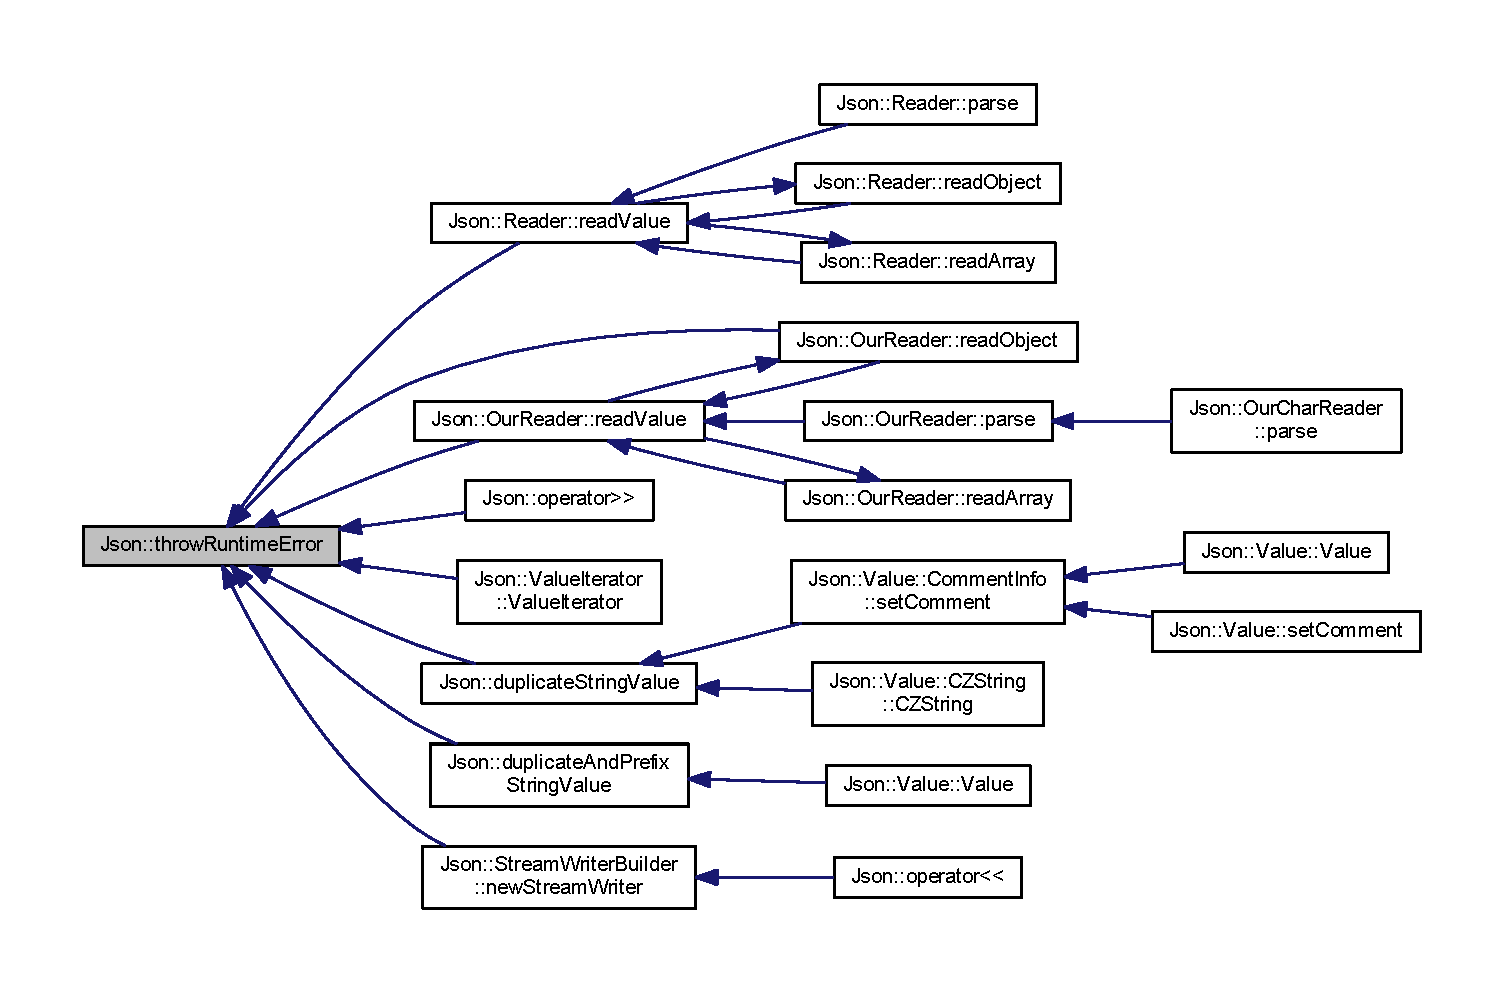
\includegraphics[width=350pt]{namespace_json_a0ab7ff7f99788262d92d9ff3d924e065_icgraph}
\end{center}
\end{figure}
\mbox{\Hypertarget{namespace_json_ac1ffd21a9e55122014353c773ccc496e}\label{namespace_json_ac1ffd21a9e55122014353c773ccc496e}} 
\index{Json@{Json}!uint\+To\+String@{uint\+To\+String}}
\index{uint\+To\+String@{uint\+To\+String}!Json@{Json}}
\subsubsection{\texorpdfstring{uint\+To\+String()}{uintToString()}}
{\footnotesize\ttfamily static void Json\+::uint\+To\+String (\begin{DoxyParamCaption}\item[{\hyperlink{namespace_json_ae202ecad69725e23443f465e257456d0}{Largest\+U\+Int}}]{value,  }\item[{char $\ast$\&}]{current }\end{DoxyParamCaption})\hspace{0.3cm}{\ttfamily [inline]}, {\ttfamily [static]}}

Converts an unsigned integer to string. 
\begin{DoxyParams}{매개변수}
{\em value} & Unsigned interger to convert to string \\
\hline
{\em current} & Input/\+Output string buffer. Must have at least uint\+To\+String\+Buffer\+Size chars free. \\
\hline
\end{DoxyParams}


jsoncpp.\+cpp 파일의 167 번째 라인에서 정의되었습니다.


\begin{DoxyCode}
167                                                                    \{
168   *--current = 0;
169   \textcolor{keywordflow}{do} \{
170     *--current = \textcolor{keyword}{static\_cast<}\textcolor{keywordtype}{char}\textcolor{keyword}{>}(value % 10U + \textcolor{keyword}{static\_cast<}\textcolor{keywordtype}{unsigned}\textcolor{keyword}{>}(\textcolor{charliteral}{'0'}));
171     value /= 10;
172   \} \textcolor{keywordflow}{while} (value != 0);
173 \}
\end{DoxyCode}
이 함수를 호출하는 함수들에 대한 그래프입니다.\+:\nopagebreak
\begin{figure}[H]
\begin{center}
\leavevmode
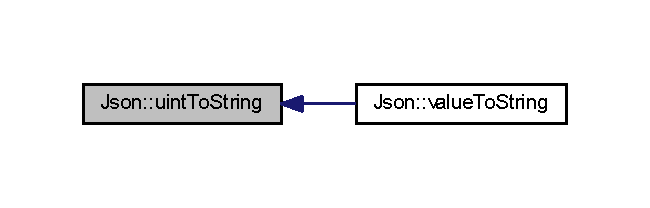
\includegraphics[width=312pt]{namespace_json_ac1ffd21a9e55122014353c773ccc496e_icgraph}
\end{center}
\end{figure}
\mbox{\Hypertarget{namespace_json_aaf777a6923bcb4cf63a2729973fe5315}\label{namespace_json_aaf777a6923bcb4cf63a2729973fe5315}} 
\index{Json@{Json}!value\+To\+Quoted\+String@{value\+To\+Quoted\+String}}
\index{value\+To\+Quoted\+String@{value\+To\+Quoted\+String}!Json@{Json}}
\subsubsection{\texorpdfstring{value\+To\+Quoted\+String()}{valueToQuotedString()}}
{\footnotesize\ttfamily \hyperlink{json_8h_a1e723f95759de062585bc4a8fd3fa4be}{J\+S\+O\+N\+C\+P\+P\+\_\+\+S\+T\+R\+I\+NG} Json\+::value\+To\+Quoted\+String (\begin{DoxyParamCaption}\item[{const char $\ast$}]{value }\end{DoxyParamCaption})}



jsoncpp.\+cpp 파일의 4259 번째 라인에서 정의되었습니다.


\begin{DoxyCode}
4259                                                       \{
4260   \textcolor{keywordflow}{if} (value == NULL)
4261     \textcolor{keywordflow}{return} \textcolor{stringliteral}{""};
4262   \textcolor{comment}{// Not sure how to handle unicode...}
4263   \textcolor{keywordflow}{if} (strpbrk(value, \textcolor{stringliteral}{"\(\backslash\)"\(\backslash\)\(\backslash\)\(\backslash\)b\(\backslash\)f\(\backslash\)n\(\backslash\)r\(\backslash\)t"}) == NULL &&
4264       !\hyperlink{namespace_json_aa11b210ff98a4f4dd4e2df19260f8c3a}{containsControlCharacter}(value))
4265     \textcolor{keywordflow}{return} \hyperlink{json-forwards_8h_a1e723f95759de062585bc4a8fd3fa4be}{JSONCPP\_STRING}(\textcolor{stringliteral}{"\(\backslash\)""}) + value + \textcolor{stringliteral}{"\(\backslash\)""};
4266   \textcolor{comment}{// We have to walk value and escape any special characters.}
4267   \textcolor{comment}{// Appending to JSONCPP\_STRING is not efficient, but this should be rare.}
4268   \textcolor{comment}{// (Note: forward slashes are *not* rare, but I am not escaping them.)}
4269   JSONCPP\_STRING::size\_type maxsize =
4270       strlen(value) * 2 + 3; \textcolor{comment}{// allescaped+quotes+NULL}
4271   \hyperlink{json-forwards_8h_a1e723f95759de062585bc4a8fd3fa4be}{JSONCPP\_STRING} result;
4272   result.reserve(maxsize); \textcolor{comment}{// to avoid lots of mallocs}
4273   result += \textcolor{stringliteral}{"\(\backslash\)""};
4274   \textcolor{keywordflow}{for} (\textcolor{keyword}{const} \textcolor{keywordtype}{char}* c = value; *c != 0; ++c) \{
4275     \textcolor{keywordflow}{switch} (*c) \{
4276     \textcolor{keywordflow}{case} \textcolor{charliteral}{'\(\backslash\)"'}:
4277       result += \textcolor{stringliteral}{"\(\backslash\)\(\backslash\)\(\backslash\)""};
4278       \textcolor{keywordflow}{break};
4279     \textcolor{keywordflow}{case} \textcolor{charliteral}{'\(\backslash\)\(\backslash\)'}:
4280       result += \textcolor{stringliteral}{"\(\backslash\)\(\backslash\)\(\backslash\)\(\backslash\)"};
4281       \textcolor{keywordflow}{break};
4282     \textcolor{keywordflow}{case} \textcolor{charliteral}{'\(\backslash\)b'}:
4283       result += \textcolor{stringliteral}{"\(\backslash\)\(\backslash\)b"};
4284       \textcolor{keywordflow}{break};
4285     \textcolor{keywordflow}{case} \textcolor{charliteral}{'\(\backslash\)f'}:
4286       result += \textcolor{stringliteral}{"\(\backslash\)\(\backslash\)f"};
4287       \textcolor{keywordflow}{break};
4288     \textcolor{keywordflow}{case} \textcolor{charliteral}{'\(\backslash\)n'}:
4289       result += \textcolor{stringliteral}{"\(\backslash\)\(\backslash\)n"};
4290       \textcolor{keywordflow}{break};
4291     \textcolor{keywordflow}{case} \textcolor{charliteral}{'\(\backslash\)r'}:
4292       result += \textcolor{stringliteral}{"\(\backslash\)\(\backslash\)r"};
4293       \textcolor{keywordflow}{break};
4294     \textcolor{keywordflow}{case} \textcolor{charliteral}{'\(\backslash\)t'}:
4295       result += \textcolor{stringliteral}{"\(\backslash\)\(\backslash\)t"};
4296       \textcolor{keywordflow}{break};
4297     \textcolor{comment}{// case '/':}
4298     \textcolor{comment}{// Even though \(\backslash\)/ is considered a legal escape in JSON, a bare}
4299     \textcolor{comment}{// slash is also legal, so I see no reason to escape it.}
4300     \textcolor{comment}{// (I hope I am not misunderstanding something.}
4301     \textcolor{comment}{// blep notes: actually escaping \(\backslash\)/ may be useful in javascript to avoid </}
4302     \textcolor{comment}{// sequence.}
4303     \textcolor{comment}{// Should add a flag to allow this compatibility mode and prevent this}
4304     \textcolor{comment}{// sequence from occurring.}
4305     \textcolor{keywordflow}{default}:
4306       \textcolor{keywordflow}{if} (\hyperlink{namespace_json_a0381e631737f51331065a388f4f59197}{isControlCharacter}(*c)) \{
4307         \hyperlink{json-forwards_8h_a1d06ac2ca63c8c521f41231dfda0e6b3}{JSONCPP\_OSTRINGSTREAM} oss;
4308         oss << \textcolor{stringliteral}{"\(\backslash\)\(\backslash\)u"} << std::hex << std::uppercase << std::setfill(\textcolor{charliteral}{'0'})
4309             << std::setw(4) << \textcolor{keyword}{static\_cast<}\textcolor{keywordtype}{int}\textcolor{keyword}{>}(*c);
4310         result += oss.str();
4311       \} \textcolor{keywordflow}{else} \{
4312         result += *c;
4313       \}
4314       \textcolor{keywordflow}{break};
4315     \}
4316   \}
4317   result += \textcolor{stringliteral}{"\(\backslash\)""};
4318   \textcolor{keywordflow}{return} result;
4319 \}
\end{DoxyCode}
이 함수 내부에서 호출하는 함수들에 대한 그래프입니다.\+:\nopagebreak
\begin{figure}[H]
\begin{center}
\leavevmode
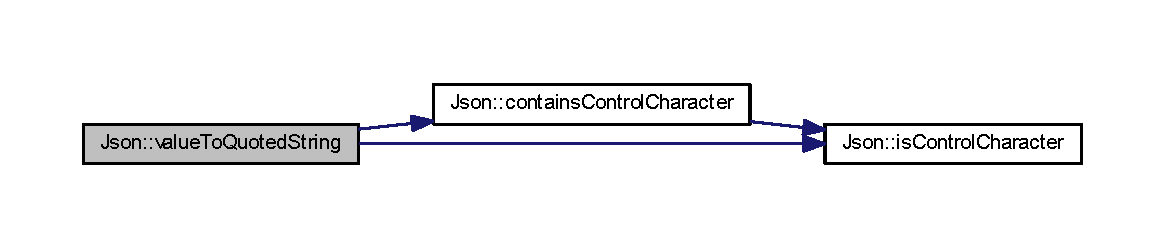
\includegraphics[width=350pt]{namespace_json_aaf777a6923bcb4cf63a2729973fe5315_cgraph}
\end{center}
\end{figure}
이 함수를 호출하는 함수들에 대한 그래프입니다.\+:\nopagebreak
\begin{figure}[H]
\begin{center}
\leavevmode
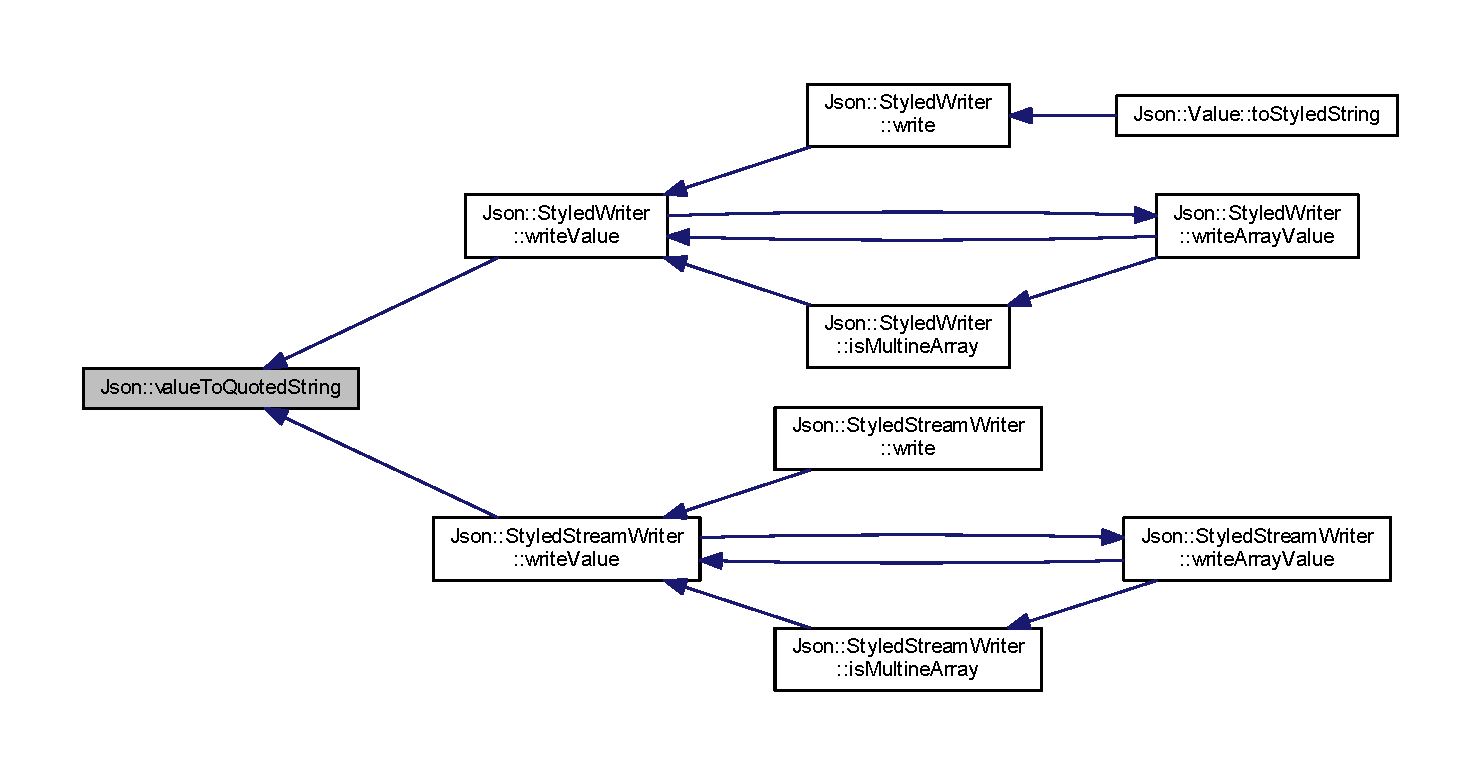
\includegraphics[width=350pt]{namespace_json_aaf777a6923bcb4cf63a2729973fe5315_icgraph}
\end{center}
\end{figure}
\mbox{\Hypertarget{namespace_json_a29aff81733b8fdaabf3f1acfc3ad339f}\label{namespace_json_a29aff81733b8fdaabf3f1acfc3ad339f}} 
\index{Json@{Json}!value\+To\+Quoted\+StringN@{value\+To\+Quoted\+StringN}}
\index{value\+To\+Quoted\+StringN@{value\+To\+Quoted\+StringN}!Json@{Json}}
\subsubsection{\texorpdfstring{value\+To\+Quoted\+String\+N()}{valueToQuotedStringN()}}
{\footnotesize\ttfamily static \hyperlink{json_8h_a1e723f95759de062585bc4a8fd3fa4be}{J\+S\+O\+N\+C\+P\+P\+\_\+\+S\+T\+R\+I\+NG} Json\+::value\+To\+Quoted\+StringN (\begin{DoxyParamCaption}\item[{const char $\ast$}]{value,  }\item[{unsigned}]{length }\end{DoxyParamCaption})\hspace{0.3cm}{\ttfamily [static]}}



jsoncpp.\+cpp 파일의 4336 번째 라인에서 정의되었습니다.


\begin{DoxyCode}
4336                                                                                \{
4337   \textcolor{keywordflow}{if} (value == NULL)
4338     \textcolor{keywordflow}{return} \textcolor{stringliteral}{""};
4339   \textcolor{comment}{// Not sure how to handle unicode...}
4340   \textcolor{keywordflow}{if} (\hyperlink{namespace_json_a7492156d0c7d2dd2f672acacfb240320}{strnpbrk}(value, \textcolor{stringliteral}{"\(\backslash\)"\(\backslash\)\(\backslash\)\(\backslash\)b\(\backslash\)f\(\backslash\)n\(\backslash\)r\(\backslash\)t"}, length) == NULL &&
4341       !\hyperlink{namespace_json_ae8a357381f264cf28f46449e79ab1dea}{containsControlCharacter0}(value, length))
4342     \textcolor{keywordflow}{return} \hyperlink{json-forwards_8h_a1e723f95759de062585bc4a8fd3fa4be}{JSONCPP\_STRING}(\textcolor{stringliteral}{"\(\backslash\)""}) + value + \textcolor{stringliteral}{"\(\backslash\)""};
4343   \textcolor{comment}{// We have to walk value and escape any special characters.}
4344   \textcolor{comment}{// Appending to JSONCPP\_STRING is not efficient, but this should be rare.}
4345   \textcolor{comment}{// (Note: forward slashes are *not* rare, but I am not escaping them.)}
4346   JSONCPP\_STRING::size\_type maxsize =
4347       length * 2 + 3; \textcolor{comment}{// allescaped+quotes+NULL}
4348   \hyperlink{json-forwards_8h_a1e723f95759de062585bc4a8fd3fa4be}{JSONCPP\_STRING} result;
4349   result.reserve(maxsize); \textcolor{comment}{// to avoid lots of mallocs}
4350   result += \textcolor{stringliteral}{"\(\backslash\)""};
4351   \textcolor{keywordtype}{char} \textcolor{keyword}{const}* end = value + length;
4352   \textcolor{keywordflow}{for} (\textcolor{keyword}{const} \textcolor{keywordtype}{char}* c = value; c != end; ++c) \{
4353     \textcolor{keywordflow}{switch} (*c) \{
4354     \textcolor{keywordflow}{case} \textcolor{charliteral}{'\(\backslash\)"'}:
4355       result += \textcolor{stringliteral}{"\(\backslash\)\(\backslash\)\(\backslash\)""};
4356       \textcolor{keywordflow}{break};
4357     \textcolor{keywordflow}{case} \textcolor{charliteral}{'\(\backslash\)\(\backslash\)'}:
4358       result += \textcolor{stringliteral}{"\(\backslash\)\(\backslash\)\(\backslash\)\(\backslash\)"};
4359       \textcolor{keywordflow}{break};
4360     \textcolor{keywordflow}{case} \textcolor{charliteral}{'\(\backslash\)b'}:
4361       result += \textcolor{stringliteral}{"\(\backslash\)\(\backslash\)b"};
4362       \textcolor{keywordflow}{break};
4363     \textcolor{keywordflow}{case} \textcolor{charliteral}{'\(\backslash\)f'}:
4364       result += \textcolor{stringliteral}{"\(\backslash\)\(\backslash\)f"};
4365       \textcolor{keywordflow}{break};
4366     \textcolor{keywordflow}{case} \textcolor{charliteral}{'\(\backslash\)n'}:
4367       result += \textcolor{stringliteral}{"\(\backslash\)\(\backslash\)n"};
4368       \textcolor{keywordflow}{break};
4369     \textcolor{keywordflow}{case} \textcolor{charliteral}{'\(\backslash\)r'}:
4370       result += \textcolor{stringliteral}{"\(\backslash\)\(\backslash\)r"};
4371       \textcolor{keywordflow}{break};
4372     \textcolor{keywordflow}{case} \textcolor{charliteral}{'\(\backslash\)t'}:
4373       result += \textcolor{stringliteral}{"\(\backslash\)\(\backslash\)t"};
4374       \textcolor{keywordflow}{break};
4375     \textcolor{comment}{// case '/':}
4376     \textcolor{comment}{// Even though \(\backslash\)/ is considered a legal escape in JSON, a bare}
4377     \textcolor{comment}{// slash is also legal, so I see no reason to escape it.}
4378     \textcolor{comment}{// (I hope I am not misunderstanding something.)}
4379     \textcolor{comment}{// blep notes: actually escaping \(\backslash\)/ may be useful in javascript to avoid </}
4380     \textcolor{comment}{// sequence.}
4381     \textcolor{comment}{// Should add a flag to allow this compatibility mode and prevent this}
4382     \textcolor{comment}{// sequence from occurring.}
4383     \textcolor{keywordflow}{default}:
4384       \textcolor{keywordflow}{if} ((\hyperlink{namespace_json_a0381e631737f51331065a388f4f59197}{isControlCharacter}(*c)) || (*c == 0)) \{
4385         \hyperlink{json-forwards_8h_a1d06ac2ca63c8c521f41231dfda0e6b3}{JSONCPP\_OSTRINGSTREAM} oss;
4386         oss << \textcolor{stringliteral}{"\(\backslash\)\(\backslash\)u"} << std::hex << std::uppercase << std::setfill(\textcolor{charliteral}{'0'})
4387             << std::setw(4) << \textcolor{keyword}{static\_cast<}\textcolor{keywordtype}{int}\textcolor{keyword}{>}(*c);
4388         result += oss.str();
4389       \} \textcolor{keywordflow}{else} \{
4390         result += *c;
4391       \}
4392       \textcolor{keywordflow}{break};
4393     \}
4394   \}
4395   result += \textcolor{stringliteral}{"\(\backslash\)""};
4396   \textcolor{keywordflow}{return} result;
4397 \}
\end{DoxyCode}
이 함수 내부에서 호출하는 함수들에 대한 그래프입니다.\+:\nopagebreak
\begin{figure}[H]
\begin{center}
\leavevmode
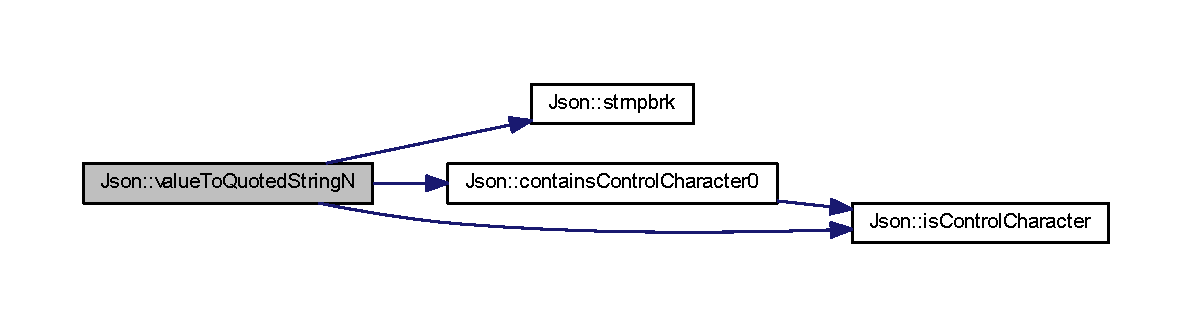
\includegraphics[width=350pt]{namespace_json_a29aff81733b8fdaabf3f1acfc3ad339f_cgraph}
\end{center}
\end{figure}
이 함수를 호출하는 함수들에 대한 그래프입니다.\+:\nopagebreak
\begin{figure}[H]
\begin{center}
\leavevmode
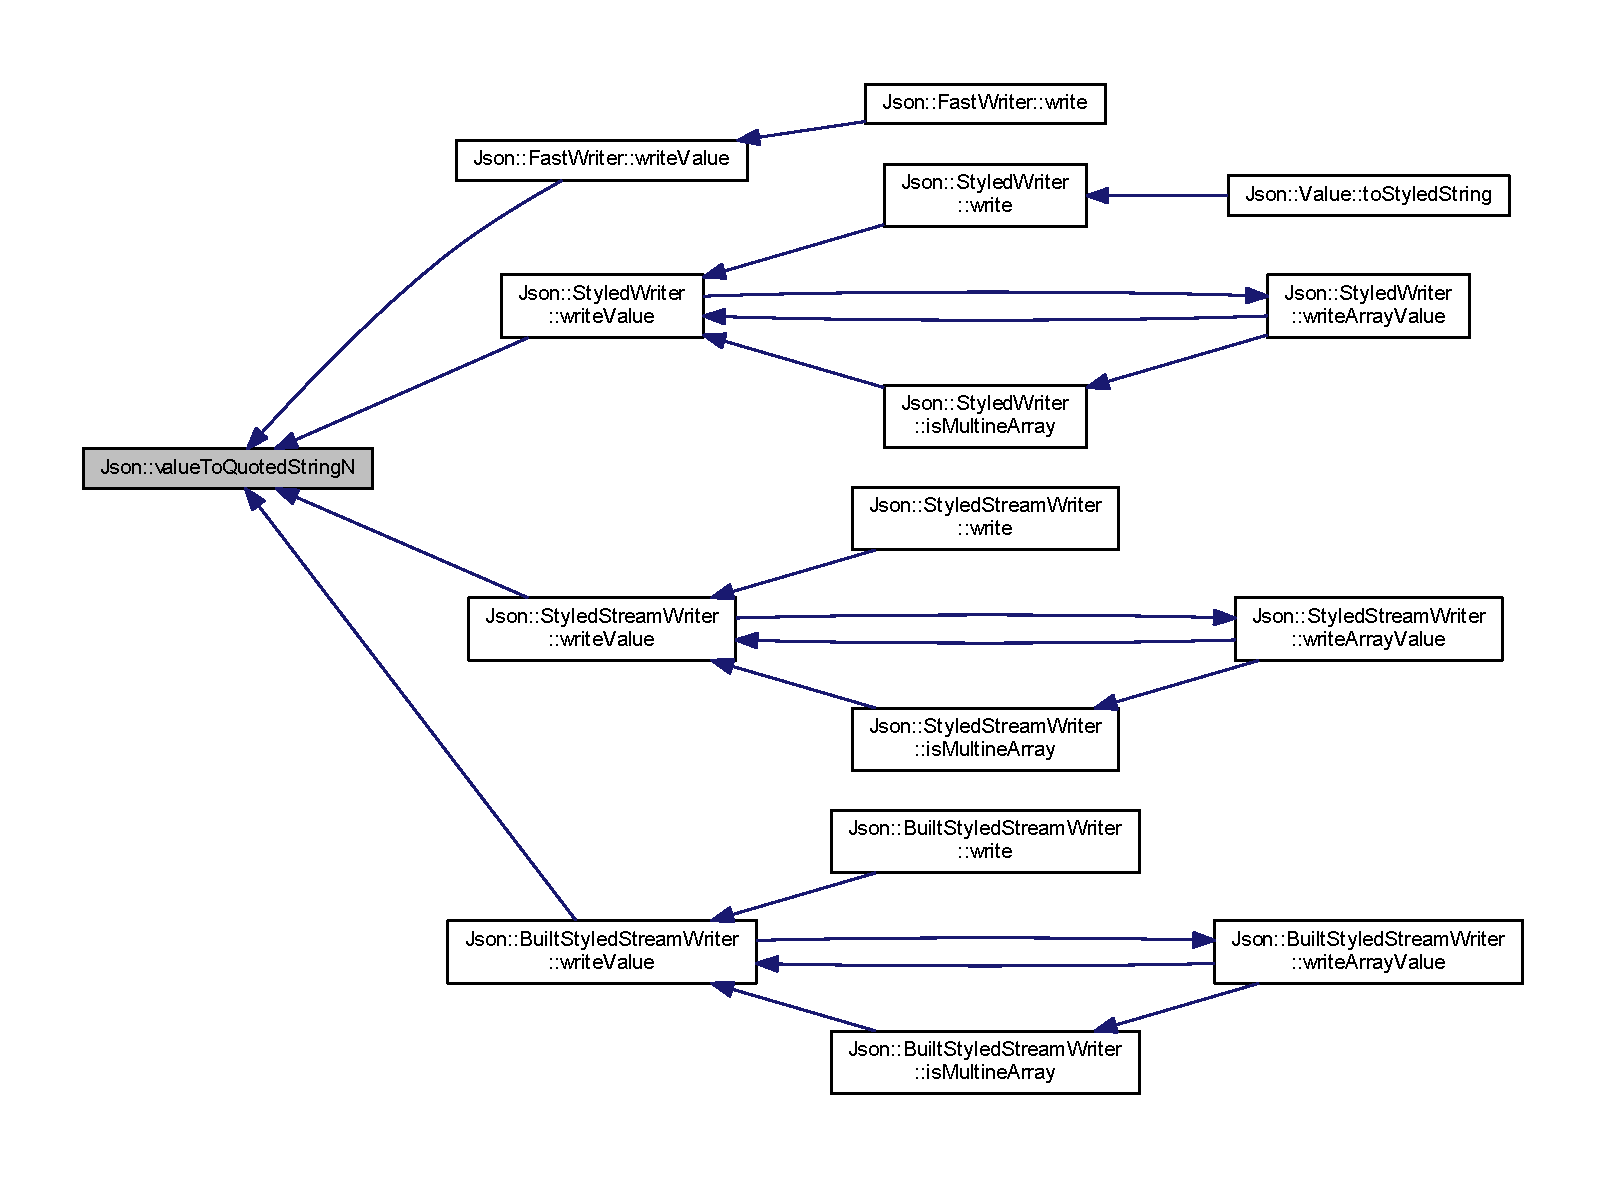
\includegraphics[width=350pt]{namespace_json_a29aff81733b8fdaabf3f1acfc3ad339f_icgraph}
\end{center}
\end{figure}
\mbox{\Hypertarget{namespace_json_a498503e8f49d6a3811e3c9f6757da60d}\label{namespace_json_a498503e8f49d6a3811e3c9f6757da60d}} 
\index{Json@{Json}!value\+To\+String@{value\+To\+String}}
\index{value\+To\+String@{value\+To\+String}!Json@{Json}}
\subsubsection{\texorpdfstring{value\+To\+String()}{valueToString()}\hspace{0.1cm}{\footnotesize\ttfamily [1/6]}}
{\footnotesize\ttfamily \hyperlink{json_8h_a1e723f95759de062585bc4a8fd3fa4be}{J\+S\+O\+N\+C\+P\+P\+\_\+\+S\+T\+R\+I\+NG} Json\+::value\+To\+String (\begin{DoxyParamCaption}\item[{\hyperlink{namespace_json_a08122e8005b706d982e48cca1e2119c7}{Int}}]{value }\end{DoxyParamCaption})}



jsoncpp.\+cpp 파일의 4207 번째 라인에서 정의되었습니다.


\begin{DoxyCode}
4207                                         \{
4208   \textcolor{keywordflow}{return} \hyperlink{namespace_json_a498503e8f49d6a3811e3c9f6757da60d}{valueToString}(\hyperlink{namespace_json_a218d880af853ce786cd985e82571d297}{LargestInt}(value));
4209 \}
\end{DoxyCode}
이 함수를 호출하는 함수들에 대한 그래프입니다.\+:\nopagebreak
\begin{figure}[H]
\begin{center}
\leavevmode
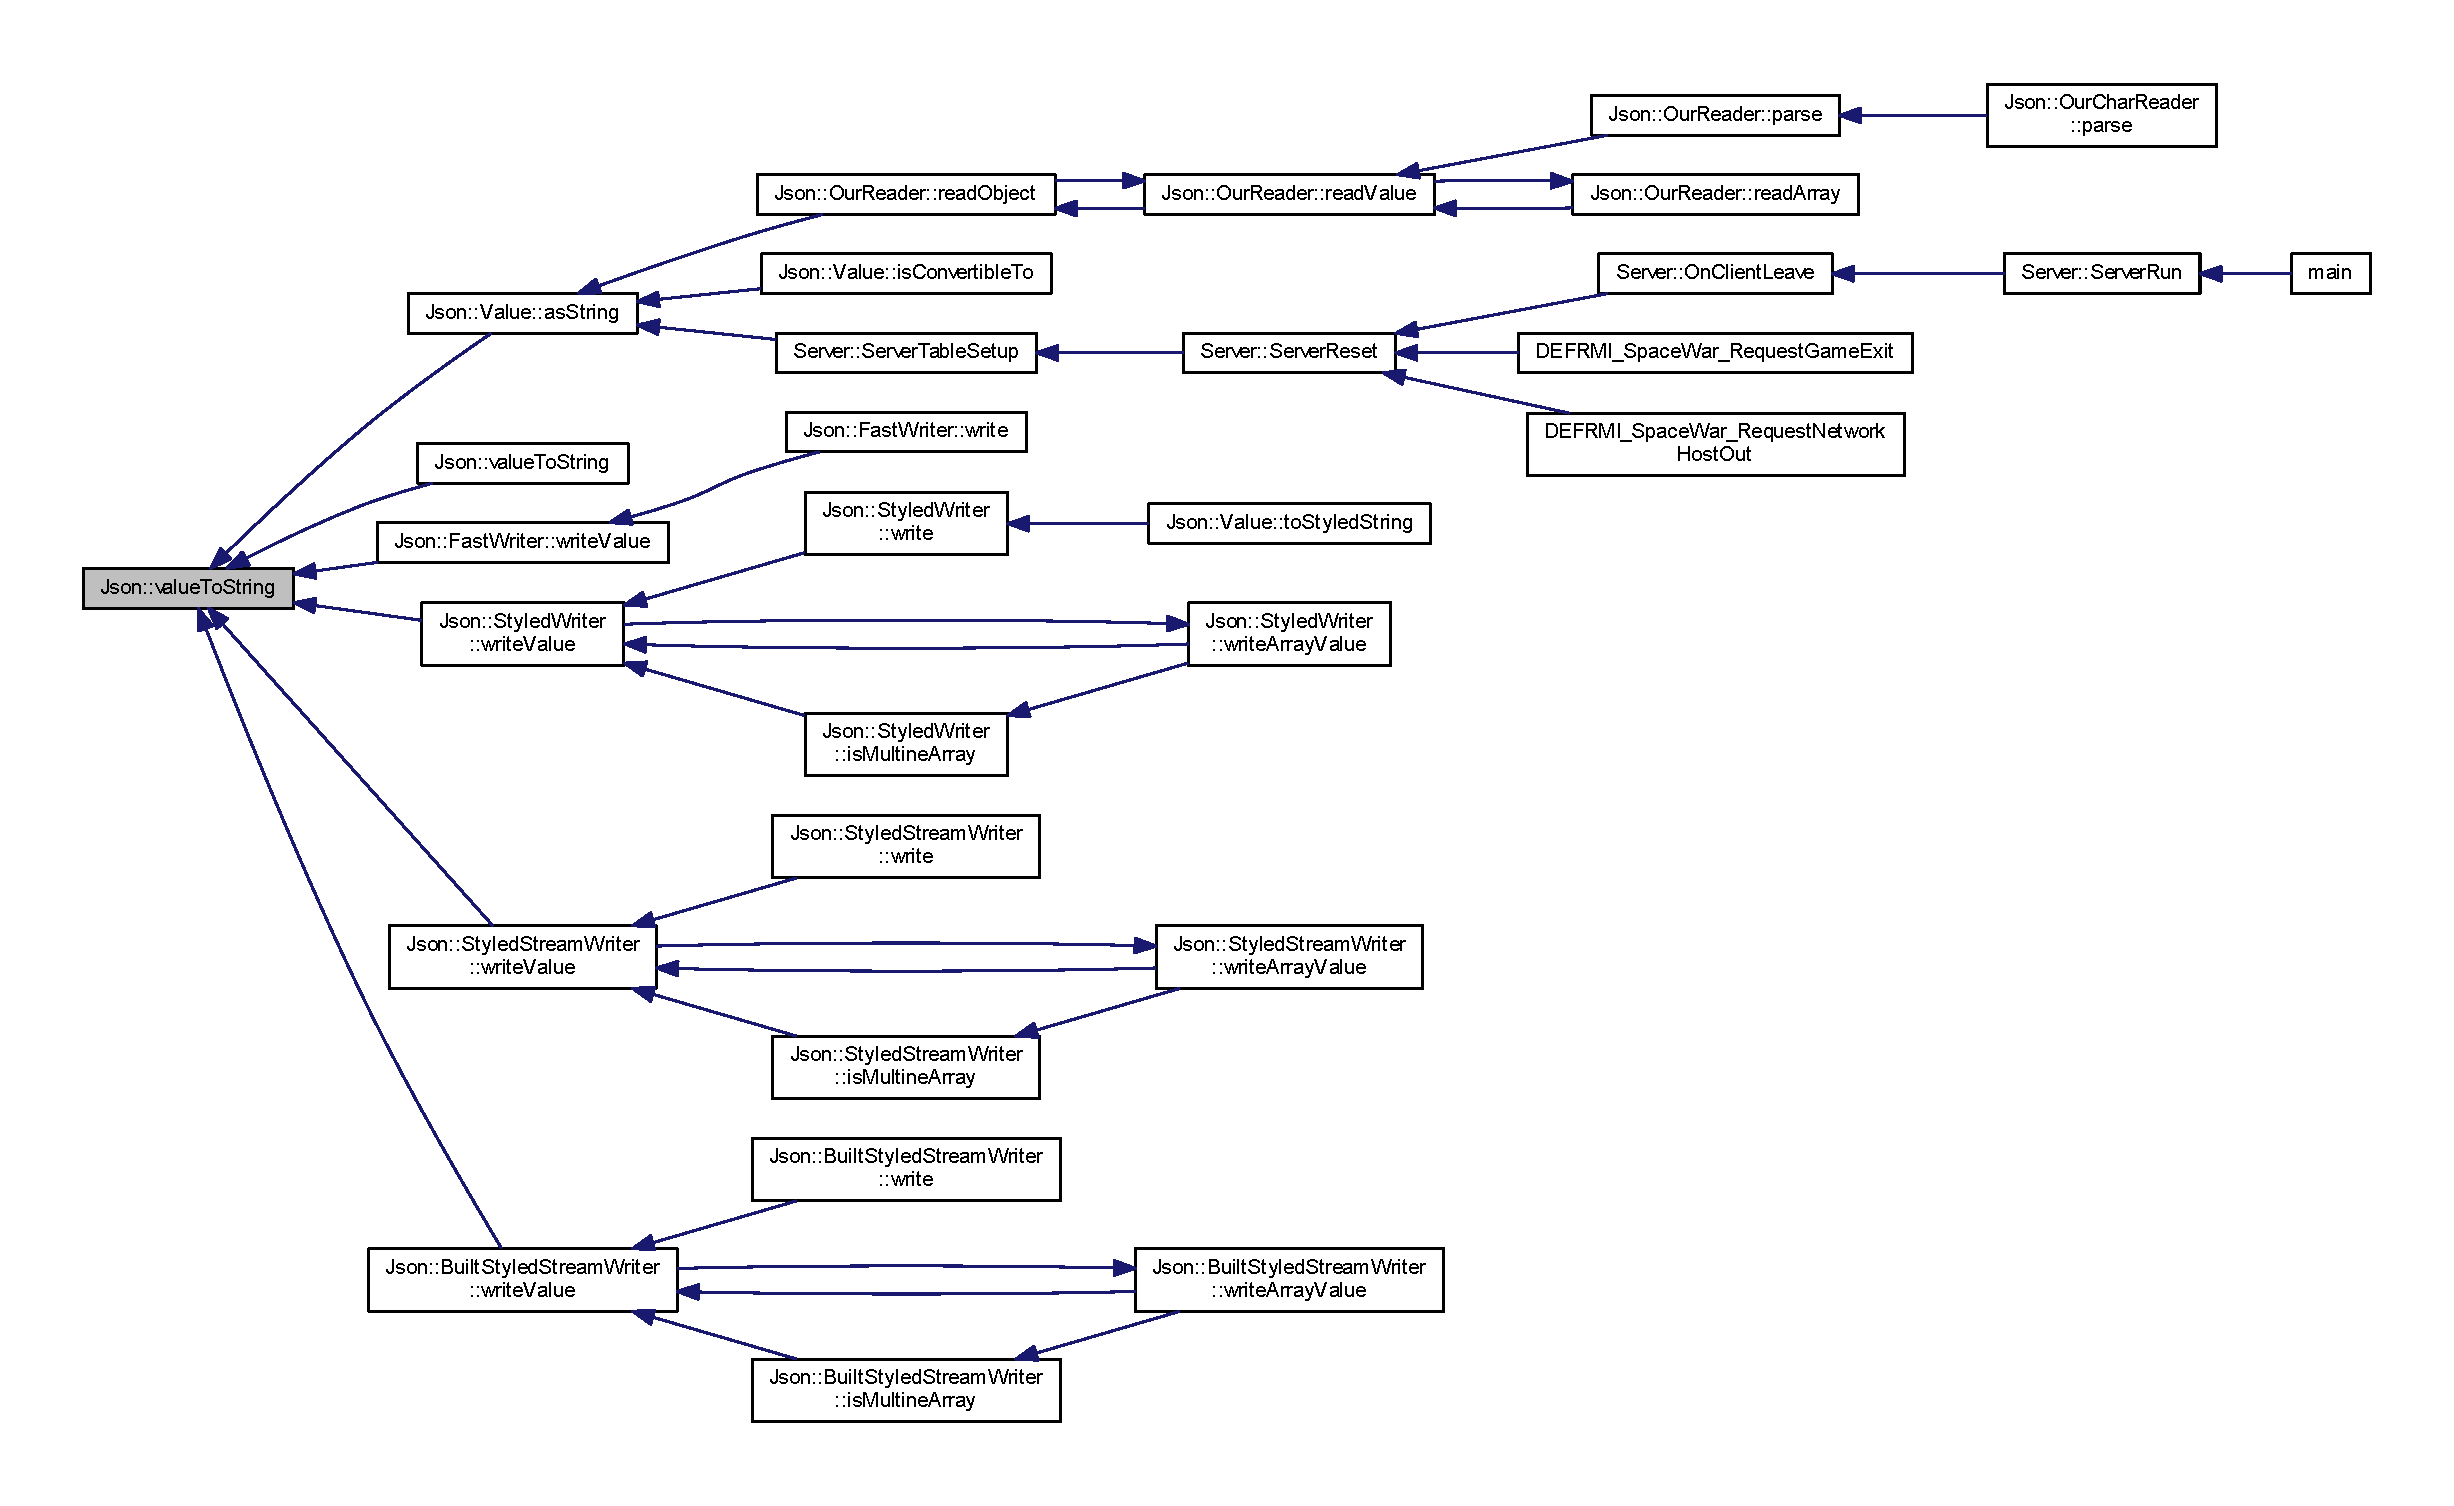
\includegraphics[width=350pt]{namespace_json_a498503e8f49d6a3811e3c9f6757da60d_icgraph}
\end{center}
\end{figure}
\mbox{\Hypertarget{namespace_json_ab2cb54f173193c8d27c3eb7f10b6e79a}\label{namespace_json_ab2cb54f173193c8d27c3eb7f10b6e79a}} 
\index{Json@{Json}!value\+To\+String@{value\+To\+String}}
\index{value\+To\+String@{value\+To\+String}!Json@{Json}}
\subsubsection{\texorpdfstring{value\+To\+String()}{valueToString()}\hspace{0.1cm}{\footnotesize\ttfamily [2/6]}}
{\footnotesize\ttfamily \hyperlink{json_8h_a1e723f95759de062585bc4a8fd3fa4be}{J\+S\+O\+N\+C\+P\+P\+\_\+\+S\+T\+R\+I\+NG} Json\+::value\+To\+String (\begin{DoxyParamCaption}\item[{\hyperlink{namespace_json_a800fb90eb6ee8d5d62b600c06f87f7d4}{U\+Int}}]{value }\end{DoxyParamCaption})}



jsoncpp.\+cpp 파일의 4211 번째 라인에서 정의되었습니다.


\begin{DoxyCode}
4211                                          \{
4212   \textcolor{keywordflow}{return} \hyperlink{namespace_json_a498503e8f49d6a3811e3c9f6757da60d}{valueToString}(\hyperlink{namespace_json_ae202ecad69725e23443f465e257456d0}{LargestUInt}(value));
4213 \}
\end{DoxyCode}
이 함수 내부에서 호출하는 함수들에 대한 그래프입니다.\+:\nopagebreak
\begin{figure}[H]
\begin{center}
\leavevmode
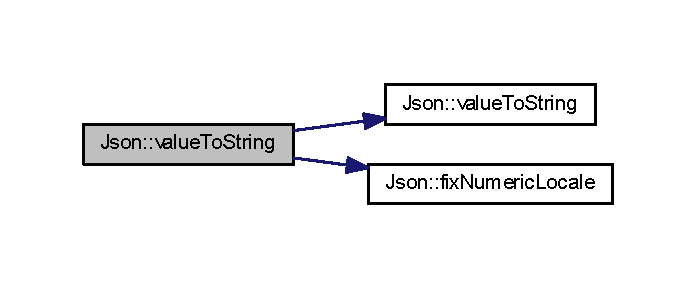
\includegraphics[width=334pt]{namespace_json_ab2cb54f173193c8d27c3eb7f10b6e79a_cgraph}
\end{center}
\end{figure}
\mbox{\Hypertarget{namespace_json_a4732517cb28d203cfd4354d05952a81b}\label{namespace_json_a4732517cb28d203cfd4354d05952a81b}} 
\index{Json@{Json}!value\+To\+String@{value\+To\+String}}
\index{value\+To\+String@{value\+To\+String}!Json@{Json}}
\subsubsection{\texorpdfstring{value\+To\+String()}{valueToString()}\hspace{0.1cm}{\footnotesize\ttfamily [3/6]}}
{\footnotesize\ttfamily \hyperlink{json_8h_a1e723f95759de062585bc4a8fd3fa4be}{J\+S\+O\+N\+C\+P\+P\+\_\+\+S\+T\+R\+I\+NG} Json\+::value\+To\+String (\begin{DoxyParamCaption}\item[{\hyperlink{namespace_json_a218d880af853ce786cd985e82571d297}{Largest\+Int}}]{value }\end{DoxyParamCaption})}



jsoncpp.\+cpp 파일의 4181 번째 라인에서 정의되었습니다.


\begin{DoxyCode}
4181                                                \{
4182   \hyperlink{namespace_json_a602bcf69c2042fb61c3b243cb16f04ca}{UIntToStringBuffer} buffer;
4183   \textcolor{keywordtype}{char}* current = buffer + \textcolor{keyword}{sizeof}(buffer);
4184   \textcolor{keywordflow}{if} (value == Value::minLargestInt) \{
4185     \hyperlink{namespace_json_ac1ffd21a9e55122014353c773ccc496e}{uintToString}(\hyperlink{namespace_json_ae202ecad69725e23443f465e257456d0}{LargestUInt}(Value::maxLargestInt) + 1, current);
4186     *--current = \textcolor{charliteral}{'-'};
4187   \} \textcolor{keywordflow}{else} \textcolor{keywordflow}{if} (value < 0) \{
4188     \hyperlink{namespace_json_ac1ffd21a9e55122014353c773ccc496e}{uintToString}(\hyperlink{namespace_json_ae202ecad69725e23443f465e257456d0}{LargestUInt}(-value), current);
4189     *--current = \textcolor{charliteral}{'-'};
4190   \} \textcolor{keywordflow}{else} \{
4191     \hyperlink{namespace_json_ac1ffd21a9e55122014353c773ccc496e}{uintToString}(\hyperlink{namespace_json_ae202ecad69725e23443f465e257456d0}{LargestUInt}(value), current);
4192   \}
4193   assert(current >= buffer);
4194   \textcolor{keywordflow}{return} current;
4195 \}
\end{DoxyCode}
이 함수 내부에서 호출하는 함수들에 대한 그래프입니다.\+:\nopagebreak
\begin{figure}[H]
\begin{center}
\leavevmode
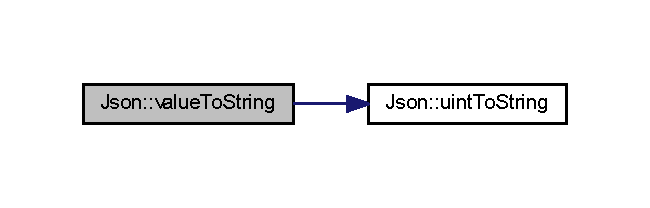
\includegraphics[width=312pt]{namespace_json_a4732517cb28d203cfd4354d05952a81b_cgraph}
\end{center}
\end{figure}
\mbox{\Hypertarget{namespace_json_a6283ea3db02efe9104ae6baff698245a}\label{namespace_json_a6283ea3db02efe9104ae6baff698245a}} 
\index{Json@{Json}!value\+To\+String@{value\+To\+String}}
\index{value\+To\+String@{value\+To\+String}!Json@{Json}}
\subsubsection{\texorpdfstring{value\+To\+String()}{valueToString()}\hspace{0.1cm}{\footnotesize\ttfamily [4/6]}}
{\footnotesize\ttfamily \hyperlink{json_8h_a1e723f95759de062585bc4a8fd3fa4be}{J\+S\+O\+N\+C\+P\+P\+\_\+\+S\+T\+R\+I\+NG} Json\+::value\+To\+String (\begin{DoxyParamCaption}\item[{\hyperlink{namespace_json_ae202ecad69725e23443f465e257456d0}{Largest\+U\+Int}}]{value }\end{DoxyParamCaption})}



jsoncpp.\+cpp 파일의 4197 번째 라인에서 정의되었습니다.


\begin{DoxyCode}
4197                                                 \{
4198   \hyperlink{namespace_json_a602bcf69c2042fb61c3b243cb16f04ca}{UIntToStringBuffer} buffer;
4199   \textcolor{keywordtype}{char}* current = buffer + \textcolor{keyword}{sizeof}(buffer);
4200   \hyperlink{namespace_json_ac1ffd21a9e55122014353c773ccc496e}{uintToString}(value, current);
4201   assert(current >= buffer);
4202   \textcolor{keywordflow}{return} current;
4203 \}
\end{DoxyCode}
이 함수 내부에서 호출하는 함수들에 대한 그래프입니다.\+:\nopagebreak
\begin{figure}[H]
\begin{center}
\leavevmode
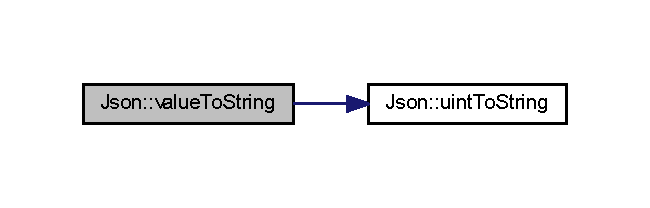
\includegraphics[width=312pt]{namespace_json_a6283ea3db02efe9104ae6baff698245a_cgraph}
\end{center}
\end{figure}
\mbox{\Hypertarget{namespace_json_a3cf0c8dbbdb898c4a6fad54670b34bd1}\label{namespace_json_a3cf0c8dbbdb898c4a6fad54670b34bd1}} 
\index{Json@{Json}!value\+To\+String@{value\+To\+String}}
\index{value\+To\+String@{value\+To\+String}!Json@{Json}}
\subsubsection{\texorpdfstring{value\+To\+String()}{valueToString()}\hspace{0.1cm}{\footnotesize\ttfamily [5/6]}}
{\footnotesize\ttfamily \hyperlink{json_8h_a1e723f95759de062585bc4a8fd3fa4be}{J\+S\+O\+N\+C\+P\+P\+\_\+\+S\+T\+R\+I\+NG} Json\+::value\+To\+String (\begin{DoxyParamCaption}\item[{double}]{value }\end{DoxyParamCaption})}



jsoncpp.\+cpp 파일의 4255 번째 라인에서 정의되었습니다.


\begin{DoxyCode}
4255 \{ \textcolor{keywordflow}{return} \hyperlink{namespace_json_a498503e8f49d6a3811e3c9f6757da60d}{valueToString}(value, \textcolor{keyword}{false}, 17); \}
\end{DoxyCode}
이 함수 내부에서 호출하는 함수들에 대한 그래프입니다.\+:\nopagebreak
\begin{figure}[H]
\begin{center}
\leavevmode
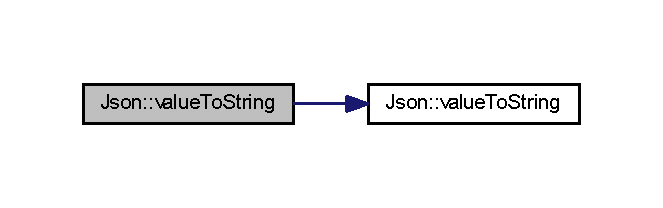
\includegraphics[width=318pt]{namespace_json_a3cf0c8dbbdb898c4a6fad54670b34bd1_cgraph}
\end{center}
\end{figure}
\mbox{\Hypertarget{namespace_json_a0a706a1fffba4fe8a8c1ef75b2dbbfab}\label{namespace_json_a0a706a1fffba4fe8a8c1ef75b2dbbfab}} 
\index{Json@{Json}!value\+To\+String@{value\+To\+String}}
\index{value\+To\+String@{value\+To\+String}!Json@{Json}}
\subsubsection{\texorpdfstring{value\+To\+String()}{valueToString()}\hspace{0.1cm}{\footnotesize\ttfamily [6/6]}}
{\footnotesize\ttfamily \hyperlink{json_8h_a1e723f95759de062585bc4a8fd3fa4be}{J\+S\+O\+N\+C\+P\+P\+\_\+\+S\+T\+R\+I\+NG} Json\+::value\+To\+String (\begin{DoxyParamCaption}\item[{bool}]{value }\end{DoxyParamCaption})}



jsoncpp.\+cpp 파일의 4257 번째 라인에서 정의되었습니다.


\begin{DoxyCode}
4257 \{ \textcolor{keywordflow}{return} value ? \textcolor{stringliteral}{"true"} : \textcolor{stringliteral}{"false"}; \}
\end{DoxyCode}
\mbox{\Hypertarget{namespace_json_a00820c0084189e2a7533531c0f250e3f}\label{namespace_json_a00820c0084189e2a7533531c0f250e3f}} 
\index{Json@{Json}!write\+String@{write\+String}}
\index{write\+String@{write\+String}!Json@{Json}}
\subsubsection{\texorpdfstring{write\+String()}{writeString()}}
{\footnotesize\ttfamily \hyperlink{json_8h_a1e723f95759de062585bc4a8fd3fa4be}{J\+S\+O\+N\+C\+P\+P\+\_\+\+S\+T\+R\+I\+NG} Json\+::write\+String (\begin{DoxyParamCaption}\item[{\hyperlink{class_json_1_1_stream_writer_1_1_factory}{Stream\+Writer\+::\+Factory} const \&}]{factory,  }\item[{\hyperlink{class_json_1_1_value}{Value} const \&}]{root }\end{DoxyParamCaption})}



Write into stringstream, then return string, for convenience. A \hyperlink{class_json_1_1_stream_writer}{Stream\+Writer} will be created from the factory, used, and then deleted. 



jsoncpp.\+cpp 파일의 5289 번째 라인에서 정의되었습니다.


\begin{DoxyCode}
5289                                                                                   \{
5290   \hyperlink{json-forwards_8h_a1d06ac2ca63c8c521f41231dfda0e6b3}{JSONCPP\_OSTRINGSTREAM} sout;
5291   \hyperlink{namespace_json_a7132404aeebfc96d7c6ad2c66260afb5}{StreamWriterPtr} \textcolor{keyword}{const} writer(builder.newStreamWriter());
5292   writer->write(root, &sout);
5293   \textcolor{keywordflow}{return} sout.str();
5294 \}
\end{DoxyCode}
이 함수 내부에서 호출하는 함수들에 대한 그래프입니다.\+:\nopagebreak
\begin{figure}[H]
\begin{center}
\leavevmode
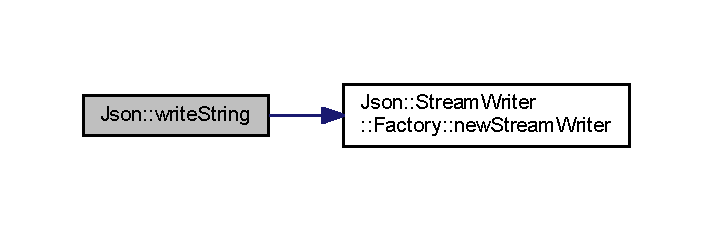
\includegraphics[width=342pt]{namespace_json_a00820c0084189e2a7533531c0f250e3f_cgraph}
\end{center}
\end{figure}


\subsection{변수 문서화}
\mbox{\Hypertarget{namespace_json_aecc0306aa526f25c5156f842182fb7fb}\label{namespace_json_aecc0306aa526f25c5156f842182fb7fb}} 
\index{Json@{Json}!max\+U\+Int64\+As\+Double@{max\+U\+Int64\+As\+Double}}
\index{max\+U\+Int64\+As\+Double@{max\+U\+Int64\+As\+Double}!Json@{Json}}
\subsubsection{\texorpdfstring{max\+U\+Int64\+As\+Double}{maxUInt64AsDouble}}
{\footnotesize\ttfamily const double Json\+::max\+U\+Int64\+As\+Double = 18446744073709551615.\+0\hspace{0.3cm}{\ttfamily [static]}}



jsoncpp.\+cpp 파일의 2509 번째 라인에서 정의되었습니다.


\hypertarget{namespace_proud}{}\section{Proud 네임스페이스 참조}
\label{namespace_proud}\index{Proud@{Proud}}
\subsection*{함수}
\begin{DoxyCompactItemize}
\item 
C\+Message \& \hyperlink{namespace_proud_aa1fd229f7228be16966e4508ed9c2a2b}{operator$<$$<$} (C\+Message \&a, const Proud\+::\+Vector3 \&b)
\item 
C\+Message \& \hyperlink{namespace_proud_a822c4aed58c18f332db22ab629174841}{operator$>$$>$} (C\+Message \&a, Proud\+::\+Vector3 \&b)
\item 
void \hyperlink{namespace_proud_a7ff9835da372ae816e45a4e4aa8ad9e3}{Append\+Text\+Out} (String \&a, Proud\+::\+Vector3 \&b)
\end{DoxyCompactItemize}


\subsection{함수 문서화}
\mbox{\Hypertarget{namespace_proud_a7ff9835da372ae816e45a4e4aa8ad9e3}\label{namespace_proud_a7ff9835da372ae816e45a4e4aa8ad9e3}} 
\index{Proud@{Proud}!Append\+Text\+Out@{Append\+Text\+Out}}
\index{Append\+Text\+Out@{Append\+Text\+Out}!Proud@{Proud}}
\subsubsection{\texorpdfstring{Append\+Text\+Out()}{AppendTextOut()}}
{\footnotesize\ttfamily void Proud\+::\+Append\+Text\+Out (\begin{DoxyParamCaption}\item[{String \&}]{a,  }\item[{Proud\+::\+Vector3 \&}]{b }\end{DoxyParamCaption})\hspace{0.3cm}{\ttfamily [inline]}}



S\+P\+\_\+\+Marshaler.\+h 파일의 28 번째 라인에서 정의되었습니다.


\begin{DoxyCode}
29     \{
30         String f;
31         f.Format(L\textcolor{stringliteral}{"\{x=%f,y=%f,z=%f\}"}, b.x, b.y, b.z);
32         a += f;
33     \}
\end{DoxyCode}
\mbox{\Hypertarget{namespace_proud_aa1fd229f7228be16966e4508ed9c2a2b}\label{namespace_proud_aa1fd229f7228be16966e4508ed9c2a2b}} 
\index{Proud@{Proud}!operator$<$$<$@{operator$<$$<$}}
\index{operator$<$$<$@{operator$<$$<$}!Proud@{Proud}}
\subsubsection{\texorpdfstring{operator$<$$<$()}{operator<<()}}
{\footnotesize\ttfamily C\+Message\& Proud\+::operator$<$$<$ (\begin{DoxyParamCaption}\item[{C\+Message \&}]{a,  }\item[{const Proud\+::\+Vector3 \&}]{b }\end{DoxyParamCaption})\hspace{0.3cm}{\ttfamily [inline]}}



S\+P\+\_\+\+Marshaler.\+h 파일의 11 번째 라인에서 정의되었습니다.


\begin{DoxyCode}
12     \{
13         a << b.x;
14         a << b.y;
15         a << b.z;
16         \textcolor{keywordflow}{return} a;
17     \}
\end{DoxyCode}
\mbox{\Hypertarget{namespace_proud_a822c4aed58c18f332db22ab629174841}\label{namespace_proud_a822c4aed58c18f332db22ab629174841}} 
\index{Proud@{Proud}!operator$>$$>$@{operator$>$$>$}}
\index{operator$>$$>$@{operator$>$$>$}!Proud@{Proud}}
\subsubsection{\texorpdfstring{operator$>$$>$()}{operator>>()}}
{\footnotesize\ttfamily C\+Message\& Proud\+::operator$>$$>$ (\begin{DoxyParamCaption}\item[{C\+Message \&}]{a,  }\item[{Proud\+::\+Vector3 \&}]{b }\end{DoxyParamCaption})\hspace{0.3cm}{\ttfamily [inline]}}



S\+P\+\_\+\+Marshaler.\+h 파일의 20 번째 라인에서 정의되었습니다.


\begin{DoxyCode}
21     \{
22         a >> b.x;
23         a >> b.y;
24         a >> b.z;
25         \textcolor{keywordflow}{return} a;
26     \}
\end{DoxyCode}

\hypertarget{namespacestd}{}\section{std 네임스페이스 참조}
\label{namespacestd}\index{std@{std}}
\subsection*{함수}
\begin{DoxyCompactItemize}
\item 
{\footnotesize template$<$$>$ }\\void \hyperlink{namespacestd_a22cc6fcbbb1f2f705c7888b615e43582}{swap} (\hyperlink{class_json_1_1_value}{Json\+::\+Value} \&a, \hyperlink{class_json_1_1_value}{Json\+::\+Value} \&b)
\begin{DoxyCompactList}\small\item\em Specialize \hyperlink{namespacestd_a22cc6fcbbb1f2f705c7888b615e43582}{std\+::swap()} for \hyperlink{class_json_1_1_value}{Json\+::\+Value}. \end{DoxyCompactList}\end{DoxyCompactItemize}


\subsection{함수 문서화}
\mbox{\Hypertarget{namespacestd_a22cc6fcbbb1f2f705c7888b615e43582}\label{namespacestd_a22cc6fcbbb1f2f705c7888b615e43582}} 
\index{std@{std}!swap@{swap}}
\index{swap@{swap}!std@{std}}
\subsubsection{\texorpdfstring{swap()}{swap()}}
{\footnotesize\ttfamily template$<$$>$ \\
void std\+::swap (\begin{DoxyParamCaption}\item[{\hyperlink{class_json_1_1_value}{Json\+::\+Value} \&}]{a,  }\item[{\hyperlink{class_json_1_1_value}{Json\+::\+Value} \&}]{b }\end{DoxyParamCaption})\hspace{0.3cm}{\ttfamily [inline]}}



Specialize \hyperlink{namespacestd_a22cc6fcbbb1f2f705c7888b615e43582}{std\+::swap()} for \hyperlink{class_json_1_1_value}{Json\+::\+Value}. 



json.\+h 파일의 1303 번째 라인에서 정의되었습니다.


\begin{DoxyCode}
1303 \{ a.\hyperlink{class_json_1_1_value_aab841120d78e296e1bc06a373345e822}{swap}(b); \}
\end{DoxyCode}
이 함수 내부에서 호출하는 함수들에 대한 그래프입니다.\+:\nopagebreak
\begin{figure}[H]
\begin{center}
\leavevmode
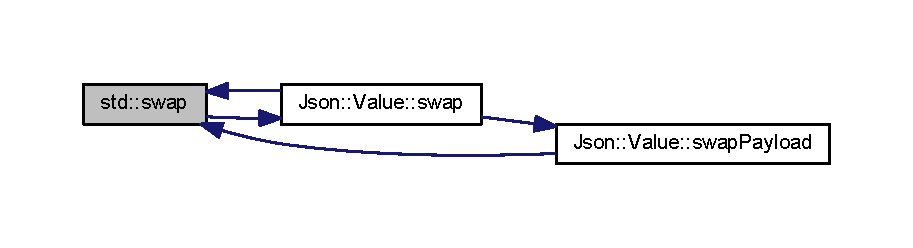
\includegraphics[width=350pt]{namespacestd_a22cc6fcbbb1f2f705c7888b615e43582_cgraph}
\end{center}
\end{figure}
이 함수를 호출하는 함수들에 대한 그래프입니다.\+:\nopagebreak
\begin{figure}[H]
\begin{center}
\leavevmode
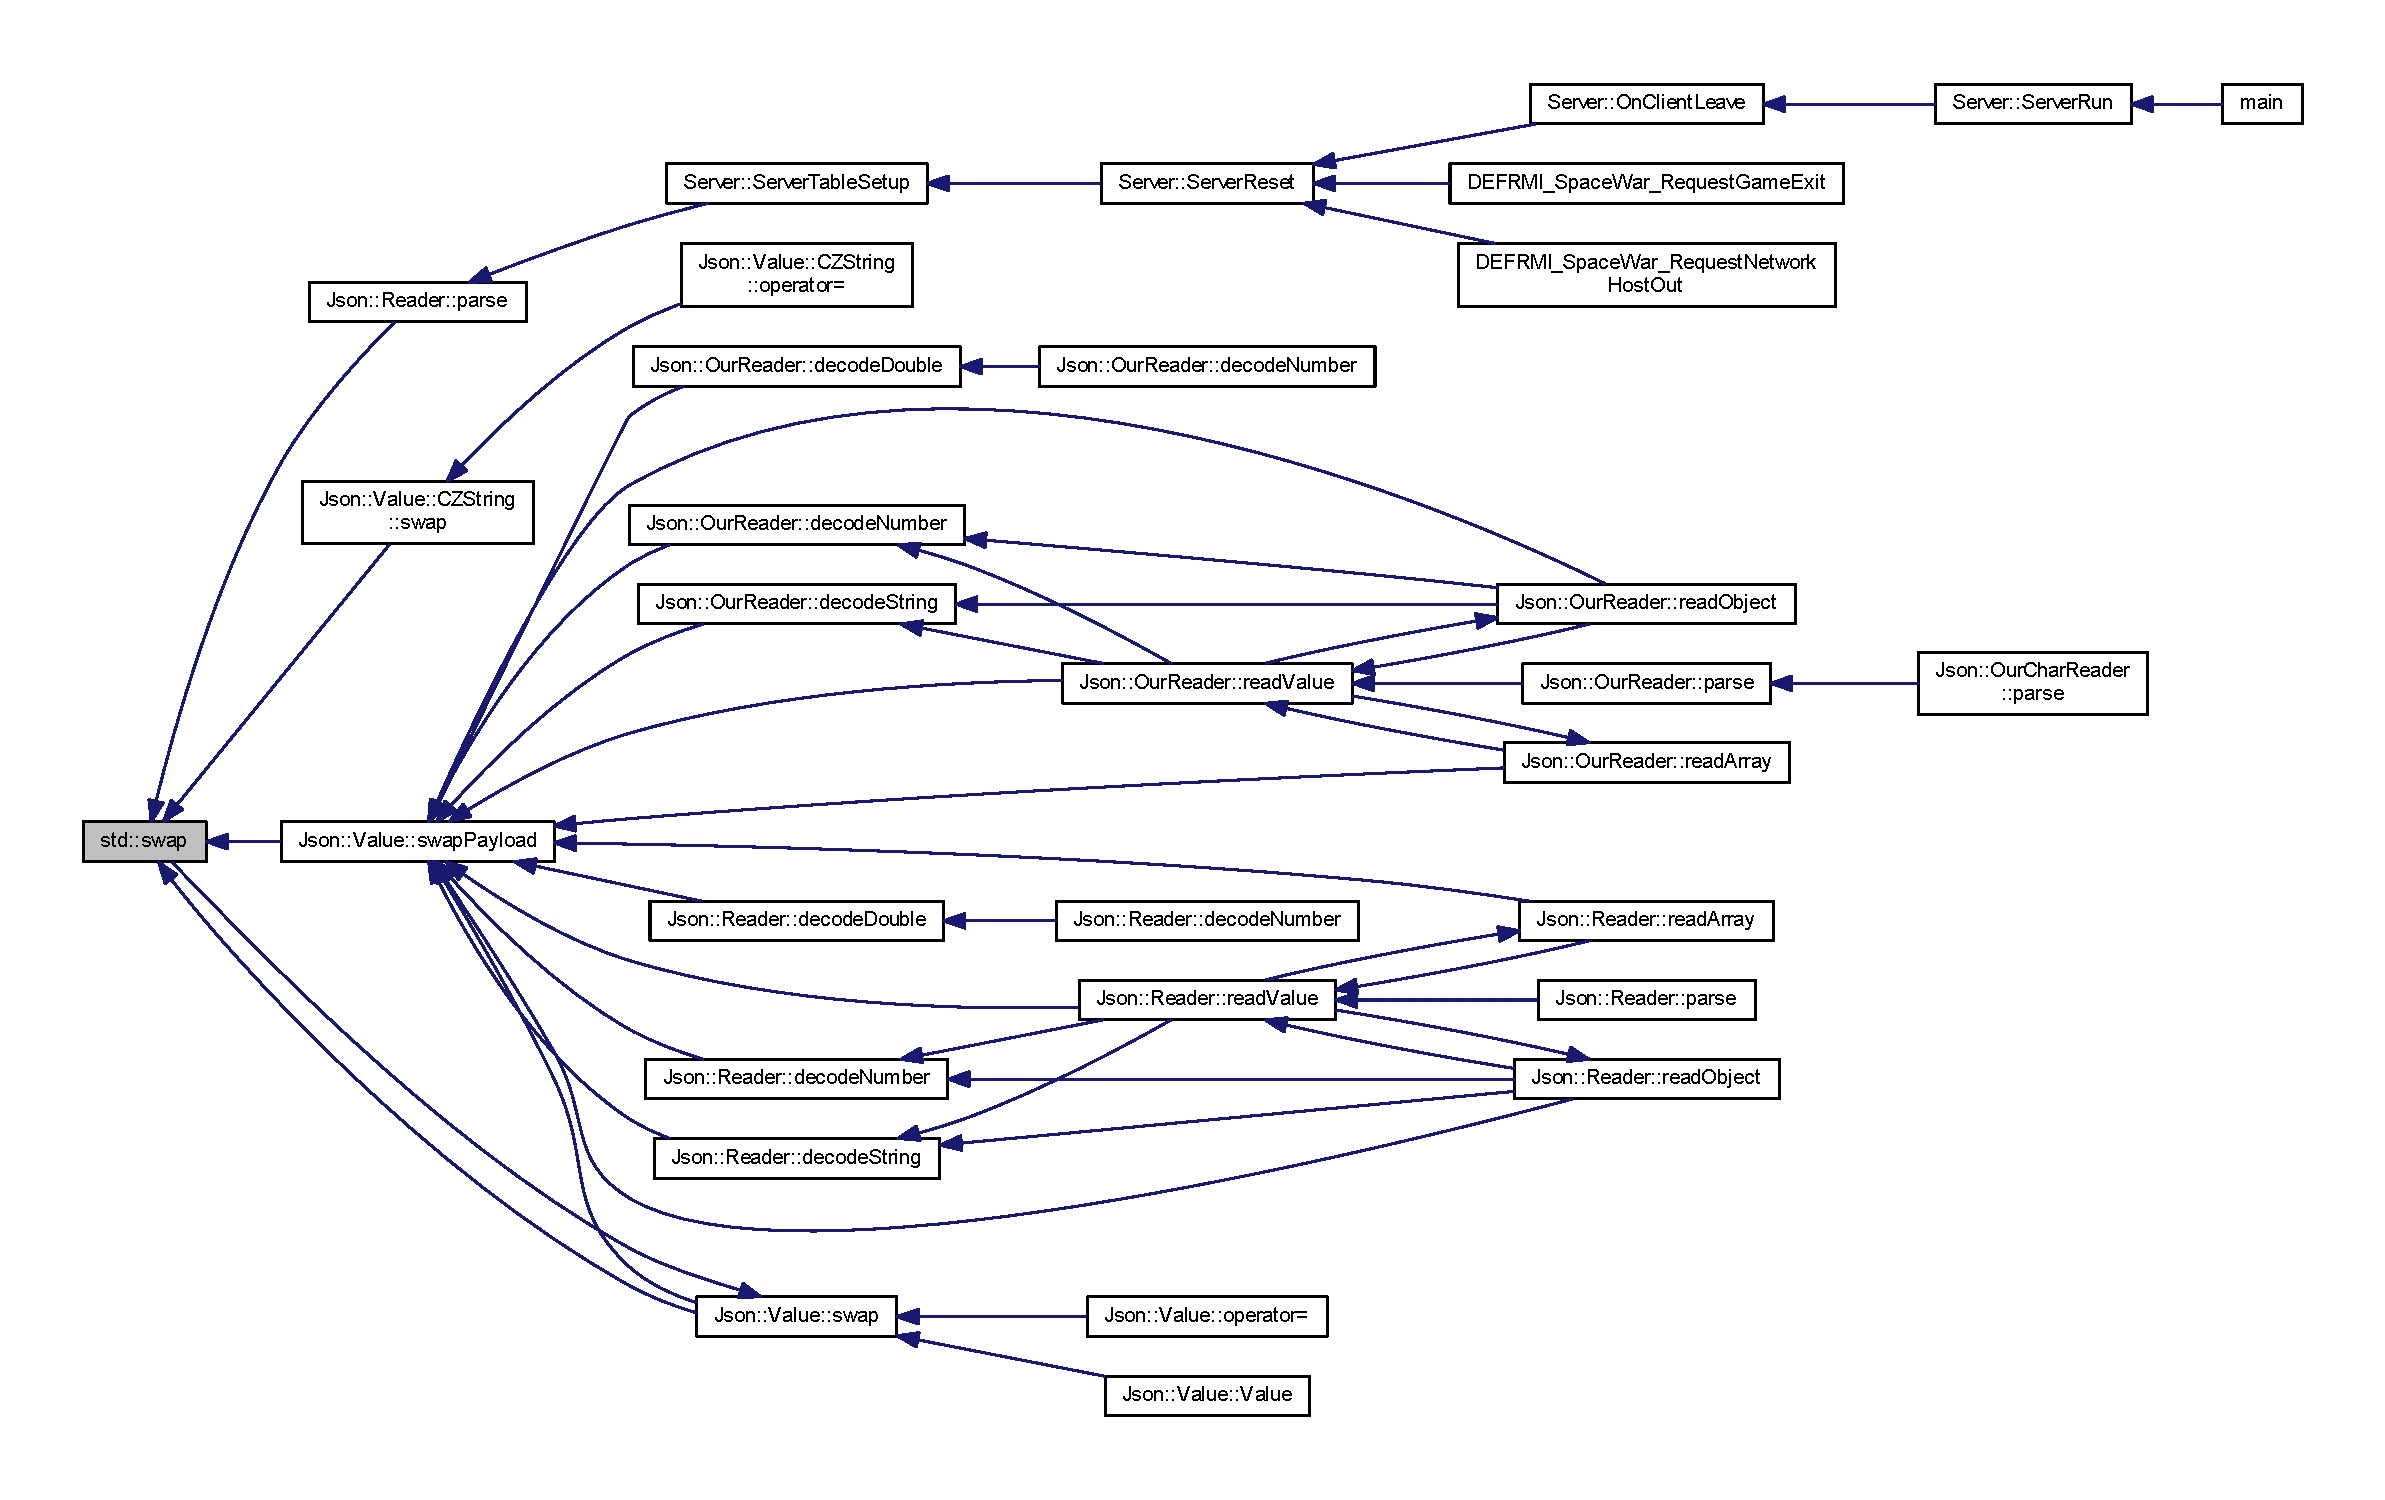
\includegraphics[width=350pt]{namespacestd_a22cc6fcbbb1f2f705c7888b615e43582_icgraph}
\end{center}
\end{figure}

\chapter{클래스 문서화}
\hypertarget{struct_json_1_1_built_styled_stream_writer}{}\section{Json\+:\+:Built\+Styled\+Stream\+Writer 구조체 참조}
\label{struct_json_1_1_built_styled_stream_writer}\index{Json\+::\+Built\+Styled\+Stream\+Writer@{Json\+::\+Built\+Styled\+Stream\+Writer}}


Json\+:\+:Built\+Styled\+Stream\+Writer에 대한 상속 다이어그램 \+: \nopagebreak
\begin{figure}[H]
\begin{center}
\leavevmode
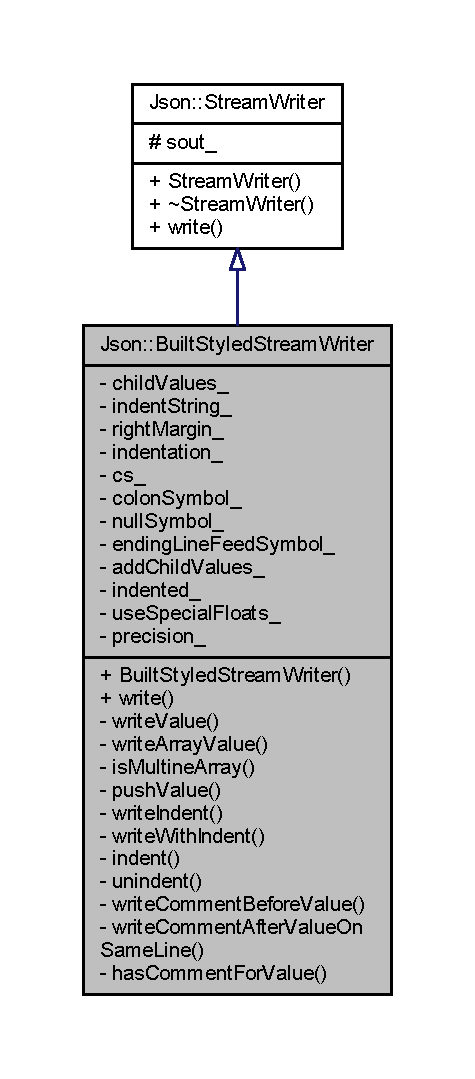
\includegraphics[width=228pt]{struct_json_1_1_built_styled_stream_writer__inherit__graph}
\end{center}
\end{figure}


Json\+:\+:Built\+Styled\+Stream\+Writer에 대한 협력 다이어그램\+:\nopagebreak
\begin{figure}[H]
\begin{center}
\leavevmode
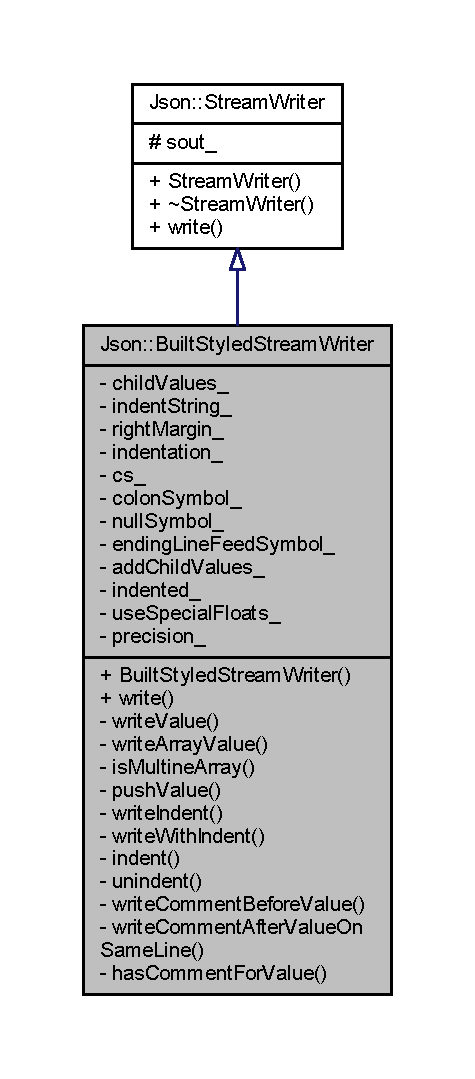
\includegraphics[width=228pt]{struct_json_1_1_built_styled_stream_writer__coll__graph}
\end{center}
\end{figure}
\subsection*{Public 멤버 함수}
\begin{DoxyCompactItemize}
\item 
\hyperlink{struct_json_1_1_built_styled_stream_writer_adf11b7d1ee3c68d096b7c662ee85948e}{Built\+Styled\+Stream\+Writer} (\hyperlink{json_8h_a1e723f95759de062585bc4a8fd3fa4be}{J\+S\+O\+N\+C\+P\+P\+\_\+\+S\+T\+R\+I\+NG} const \&indentation, \hyperlink{struct_json_1_1_comment_style_a51fc08f3518fd81eba12f340d19a3d0c}{Comment\+Style\+::\+Enum} cs, \hyperlink{json_8h_a1e723f95759de062585bc4a8fd3fa4be}{J\+S\+O\+N\+C\+P\+P\+\_\+\+S\+T\+R\+I\+NG} const \&colon\+Symbol, \hyperlink{json_8h_a1e723f95759de062585bc4a8fd3fa4be}{J\+S\+O\+N\+C\+P\+P\+\_\+\+S\+T\+R\+I\+NG} const \&null\+Symbol, \hyperlink{json_8h_a1e723f95759de062585bc4a8fd3fa4be}{J\+S\+O\+N\+C\+P\+P\+\_\+\+S\+T\+R\+I\+NG} const \&ending\+Line\+Feed\+Symbol, bool use\+Special\+Floats, unsigned int precision)
\item 
int \hyperlink{struct_json_1_1_built_styled_stream_writer_a823cdb1afabb6b0d5f39bcd5a6a6f747}{write} (\hyperlink{class_json_1_1_value}{Value} const \&root, \hyperlink{json_8h_a37a25be5fca174927780caeb280094ce}{J\+S\+O\+N\+C\+P\+P\+\_\+\+O\+S\+T\+R\+E\+AM} $\ast$sout) \hyperlink{json_8h_a824d6199c91488107e443226fa6022c5}{J\+S\+O\+N\+C\+P\+P\+\_\+\+O\+V\+E\+R\+R\+I\+DE}
\end{DoxyCompactItemize}
\subsection*{Protected 속성}
\begin{DoxyCompactItemize}
\item 
\hyperlink{json_8h_a37a25be5fca174927780caeb280094ce}{J\+S\+O\+N\+C\+P\+P\+\_\+\+O\+S\+T\+R\+E\+AM} $\ast$ \hyperlink{class_json_1_1_stream_writer_a4f5603d4228a9fa46a42cb44e5234d9b}{sout\+\_\+}
\end{DoxyCompactItemize}
\subsection*{Private 타입}
\begin{DoxyCompactItemize}
\item 
typedef std\+::vector$<$ \hyperlink{json_8h_a1e723f95759de062585bc4a8fd3fa4be}{J\+S\+O\+N\+C\+P\+P\+\_\+\+S\+T\+R\+I\+NG} $>$ \hyperlink{struct_json_1_1_built_styled_stream_writer_a63196b38400e5ce452f65ce856d47b6f}{Child\+Values}
\end{DoxyCompactItemize}
\subsection*{Private 멤버 함수}
\begin{DoxyCompactItemize}
\item 
void \hyperlink{struct_json_1_1_built_styled_stream_writer_a7c9da861861e570a51b45f270c9ff150}{write\+Value} (\hyperlink{class_json_1_1_value}{Value} const \&value)
\item 
void \hyperlink{struct_json_1_1_built_styled_stream_writer_acd20e9274bbcf7876ef3af2e7d23a31f}{write\+Array\+Value} (\hyperlink{class_json_1_1_value}{Value} const \&value)
\item 
bool \hyperlink{struct_json_1_1_built_styled_stream_writer_af423fd33b3d580506ea3efc53b05a077}{is\+Multine\+Array} (\hyperlink{class_json_1_1_value}{Value} const \&value)
\item 
void \hyperlink{struct_json_1_1_built_styled_stream_writer_a91e8535508412eea04d77c0cafdf15aa}{push\+Value} (\hyperlink{json_8h_a1e723f95759de062585bc4a8fd3fa4be}{J\+S\+O\+N\+C\+P\+P\+\_\+\+S\+T\+R\+I\+NG} const \&value)
\item 
void \hyperlink{struct_json_1_1_built_styled_stream_writer_a2b38a3714d415c4bd3b4812897130f3d}{write\+Indent} ()
\item 
void \hyperlink{struct_json_1_1_built_styled_stream_writer_a6e80e1a0d5f64df2ec48c3c3b1284990}{write\+With\+Indent} (\hyperlink{json_8h_a1e723f95759de062585bc4a8fd3fa4be}{J\+S\+O\+N\+C\+P\+P\+\_\+\+S\+T\+R\+I\+NG} const \&value)
\item 
void \hyperlink{struct_json_1_1_built_styled_stream_writer_a73e09692a2cfbd6e67836b060dc34a9f}{indent} ()
\item 
void \hyperlink{struct_json_1_1_built_styled_stream_writer_a0da6c6f603e00c8c6e38af553edd8c55}{unindent} ()
\item 
void \hyperlink{struct_json_1_1_built_styled_stream_writer_a32c4afca4e08fba79bb0a80a8010283a}{write\+Comment\+Before\+Value} (\hyperlink{class_json_1_1_value}{Value} const \&root)
\item 
void \hyperlink{struct_json_1_1_built_styled_stream_writer_a89625b134fce0255263ca40e6125742b}{write\+Comment\+After\+Value\+On\+Same\+Line} (\hyperlink{class_json_1_1_value}{Value} const \&root)
\end{DoxyCompactItemize}
\subsection*{정적 Private 멤버 함수}
\begin{DoxyCompactItemize}
\item 
static bool \hyperlink{struct_json_1_1_built_styled_stream_writer_a457c2f3c1e8c952caeb60e52477d0c9a}{has\+Comment\+For\+Value} (const \hyperlink{class_json_1_1_value}{Value} \&value)
\end{DoxyCompactItemize}
\subsection*{Private 속성}
\begin{DoxyCompactItemize}
\item 
\hyperlink{struct_json_1_1_built_styled_stream_writer_a63196b38400e5ce452f65ce856d47b6f}{Child\+Values} \hyperlink{struct_json_1_1_built_styled_stream_writer_a47d562d7874c5b1e68995bd62f575792}{child\+Values\+\_\+}
\item 
\hyperlink{json_8h_a1e723f95759de062585bc4a8fd3fa4be}{J\+S\+O\+N\+C\+P\+P\+\_\+\+S\+T\+R\+I\+NG} \hyperlink{struct_json_1_1_built_styled_stream_writer_a0f8115a4fb474ab0e9de25f10e5ca09a}{indent\+String\+\_\+}
\item 
unsigned int \hyperlink{struct_json_1_1_built_styled_stream_writer_a06a51521ccae20397f52fe3036edc602}{right\+Margin\+\_\+}
\item 
\hyperlink{json_8h_a1e723f95759de062585bc4a8fd3fa4be}{J\+S\+O\+N\+C\+P\+P\+\_\+\+S\+T\+R\+I\+NG} \hyperlink{struct_json_1_1_built_styled_stream_writer_aaa4cbad91428ceca37cbabfc2a17a92d}{indentation\+\_\+}
\item 
\hyperlink{struct_json_1_1_comment_style_a51fc08f3518fd81eba12f340d19a3d0c}{Comment\+Style\+::\+Enum} \hyperlink{struct_json_1_1_built_styled_stream_writer_a89a9c76c7531143b52785861ba21c1d4}{cs\+\_\+}
\item 
\hyperlink{json_8h_a1e723f95759de062585bc4a8fd3fa4be}{J\+S\+O\+N\+C\+P\+P\+\_\+\+S\+T\+R\+I\+NG} \hyperlink{struct_json_1_1_built_styled_stream_writer_a9f10991ddef9b77d0b580e24e71483c6}{colon\+Symbol\+\_\+}
\item 
\hyperlink{json_8h_a1e723f95759de062585bc4a8fd3fa4be}{J\+S\+O\+N\+C\+P\+P\+\_\+\+S\+T\+R\+I\+NG} \hyperlink{struct_json_1_1_built_styled_stream_writer_a6ccceadf4b1286a519a175cb59cb61d5}{null\+Symbol\+\_\+}
\item 
\hyperlink{json_8h_a1e723f95759de062585bc4a8fd3fa4be}{J\+S\+O\+N\+C\+P\+P\+\_\+\+S\+T\+R\+I\+NG} \hyperlink{struct_json_1_1_built_styled_stream_writer_a5e61a9a4b2af52b98900286c843b86f7}{ending\+Line\+Feed\+Symbol\+\_\+}
\item 
bool \hyperlink{struct_json_1_1_built_styled_stream_writer_abed9cc31da503b48798e7cea68c42e16}{add\+Child\+Values\+\_\+}\+: 1
\item 
bool \hyperlink{struct_json_1_1_built_styled_stream_writer_a6aa0ad023e623f600103631a6bca6d10}{indented\+\_\+}\+: 1
\item 
bool \hyperlink{struct_json_1_1_built_styled_stream_writer_a6f1b8694b4eb17ab8c34f6d6dd8c8a4a}{use\+Special\+Floats\+\_\+}\+: 1
\item 
unsigned int \hyperlink{struct_json_1_1_built_styled_stream_writer_a6373d8d0ae4741b64e3904e4db0eef46}{precision\+\_\+}
\end{DoxyCompactItemize}


\subsection{상세한 설명}


jsoncpp.\+cpp 파일의 4919 번째 라인에서 정의되었습니다.



\subsection{멤버 타입정의 문서화}
\mbox{\Hypertarget{struct_json_1_1_built_styled_stream_writer_a63196b38400e5ce452f65ce856d47b6f}\label{struct_json_1_1_built_styled_stream_writer_a63196b38400e5ce452f65ce856d47b6f}} 
\index{Json\+::\+Built\+Styled\+Stream\+Writer@{Json\+::\+Built\+Styled\+Stream\+Writer}!Child\+Values@{Child\+Values}}
\index{Child\+Values@{Child\+Values}!Json\+::\+Built\+Styled\+Stream\+Writer@{Json\+::\+Built\+Styled\+Stream\+Writer}}
\subsubsection{\texorpdfstring{Child\+Values}{ChildValues}}
{\footnotesize\ttfamily typedef std\+::vector$<$\hyperlink{json_8h_a1e723f95759de062585bc4a8fd3fa4be}{J\+S\+O\+N\+C\+P\+P\+\_\+\+S\+T\+R\+I\+NG}$>$ \hyperlink{struct_json_1_1_built_styled_stream_writer_a63196b38400e5ce452f65ce856d47b6f}{Json\+::\+Built\+Styled\+Stream\+Writer\+::\+Child\+Values}\hspace{0.3cm}{\ttfamily [private]}}



jsoncpp.\+cpp 파일의 4943 번째 라인에서 정의되었습니다.



\subsection{생성자 \& 소멸자 문서화}
\mbox{\Hypertarget{struct_json_1_1_built_styled_stream_writer_adf11b7d1ee3c68d096b7c662ee85948e}\label{struct_json_1_1_built_styled_stream_writer_adf11b7d1ee3c68d096b7c662ee85948e}} 
\index{Json\+::\+Built\+Styled\+Stream\+Writer@{Json\+::\+Built\+Styled\+Stream\+Writer}!Built\+Styled\+Stream\+Writer@{Built\+Styled\+Stream\+Writer}}
\index{Built\+Styled\+Stream\+Writer@{Built\+Styled\+Stream\+Writer}!Json\+::\+Built\+Styled\+Stream\+Writer@{Json\+::\+Built\+Styled\+Stream\+Writer}}
\subsubsection{\texorpdfstring{Built\+Styled\+Stream\+Writer()}{BuiltStyledStreamWriter()}}
{\footnotesize\ttfamily Json\+::\+Built\+Styled\+Stream\+Writer\+::\+Built\+Styled\+Stream\+Writer (\begin{DoxyParamCaption}\item[{\hyperlink{json_8h_a1e723f95759de062585bc4a8fd3fa4be}{J\+S\+O\+N\+C\+P\+P\+\_\+\+S\+T\+R\+I\+NG} const \&}]{indentation,  }\item[{\hyperlink{struct_json_1_1_comment_style_a51fc08f3518fd81eba12f340d19a3d0c}{Comment\+Style\+::\+Enum}}]{cs,  }\item[{\hyperlink{json_8h_a1e723f95759de062585bc4a8fd3fa4be}{J\+S\+O\+N\+C\+P\+P\+\_\+\+S\+T\+R\+I\+NG} const \&}]{colon\+Symbol,  }\item[{\hyperlink{json_8h_a1e723f95759de062585bc4a8fd3fa4be}{J\+S\+O\+N\+C\+P\+P\+\_\+\+S\+T\+R\+I\+NG} const \&}]{null\+Symbol,  }\item[{\hyperlink{json_8h_a1e723f95759de062585bc4a8fd3fa4be}{J\+S\+O\+N\+C\+P\+P\+\_\+\+S\+T\+R\+I\+NG} const \&}]{ending\+Line\+Feed\+Symbol,  }\item[{bool}]{use\+Special\+Floats,  }\item[{unsigned int}]{precision }\end{DoxyParamCaption})}



jsoncpp.\+cpp 파일의 4958 번째 라인에서 정의되었습니다.


\begin{DoxyCode}
4966   : \hyperlink{struct_json_1_1_built_styled_stream_writer_a06a51521ccae20397f52fe3036edc602}{rightMargin\_}(74)
4967   , \hyperlink{struct_json_1_1_built_styled_stream_writer_aaa4cbad91428ceca37cbabfc2a17a92d}{indentation\_}(indentation)
4968   , \hyperlink{struct_json_1_1_built_styled_stream_writer_a89a9c76c7531143b52785861ba21c1d4}{cs\_}(cs)
4969   , \hyperlink{struct_json_1_1_built_styled_stream_writer_a9f10991ddef9b77d0b580e24e71483c6}{colonSymbol\_}(colonSymbol)
4970   , \hyperlink{struct_json_1_1_built_styled_stream_writer_a6ccceadf4b1286a519a175cb59cb61d5}{nullSymbol\_}(nullSymbol)
4971   , \hyperlink{struct_json_1_1_built_styled_stream_writer_a5e61a9a4b2af52b98900286c843b86f7}{endingLineFeedSymbol\_}(endingLineFeedSymbol)
4972   , \hyperlink{struct_json_1_1_built_styled_stream_writer_abed9cc31da503b48798e7cea68c42e16}{addChildValues\_}(\textcolor{keyword}{false})
4973   , \hyperlink{struct_json_1_1_built_styled_stream_writer_a6aa0ad023e623f600103631a6bca6d10}{indented\_}(\textcolor{keyword}{false})
4974   , \hyperlink{struct_json_1_1_built_styled_stream_writer_a6f1b8694b4eb17ab8c34f6d6dd8c8a4a}{useSpecialFloats\_}(useSpecialFloats)
4975   , \hyperlink{struct_json_1_1_built_styled_stream_writer_a6373d8d0ae4741b64e3904e4db0eef46}{precision\_}(precision)
4976 \{
4977 \}
\end{DoxyCode}


\subsection{멤버 함수 문서화}
\mbox{\Hypertarget{struct_json_1_1_built_styled_stream_writer_a457c2f3c1e8c952caeb60e52477d0c9a}\label{struct_json_1_1_built_styled_stream_writer_a457c2f3c1e8c952caeb60e52477d0c9a}} 
\index{Json\+::\+Built\+Styled\+Stream\+Writer@{Json\+::\+Built\+Styled\+Stream\+Writer}!has\+Comment\+For\+Value@{has\+Comment\+For\+Value}}
\index{has\+Comment\+For\+Value@{has\+Comment\+For\+Value}!Json\+::\+Built\+Styled\+Stream\+Writer@{Json\+::\+Built\+Styled\+Stream\+Writer}}
\subsubsection{\texorpdfstring{has\+Comment\+For\+Value()}{hasCommentForValue()}}
{\footnotesize\ttfamily bool Json\+::\+Built\+Styled\+Stream\+Writer\+::has\+Comment\+For\+Value (\begin{DoxyParamCaption}\item[{const \hyperlink{class_json_1_1_value}{Value} \&}]{value }\end{DoxyParamCaption})\hspace{0.3cm}{\ttfamily [static]}, {\ttfamily [private]}}



jsoncpp.\+cpp 파일의 5189 번째 라인에서 정의되었습니다.


\begin{DoxyCode}
5189                                                                    \{
5190   \textcolor{keywordflow}{return} value.\hyperlink{class_json_1_1_value_a65d8e3ab6a5871cbd019a3e0f0b944a3}{hasComment}(\hyperlink{namespace_json_a4fc417c23905b2ae9e2c47d197a45351a52f1733775460517b2ea6bedf4906d52}{commentBefore}) ||
5191          value.\hyperlink{class_json_1_1_value_a65d8e3ab6a5871cbd019a3e0f0b944a3}{hasComment}(\hyperlink{namespace_json_a4fc417c23905b2ae9e2c47d197a45351a008a230a0586de54f30b76afe70fdcfa}{commentAfterOnSameLine}) ||
5192          value.\hyperlink{class_json_1_1_value_a65d8e3ab6a5871cbd019a3e0f0b944a3}{hasComment}(\hyperlink{namespace_json_a4fc417c23905b2ae9e2c47d197a45351ac5784ca53b12250888ddb642b06aebef}{commentAfter});
5193 \}
\end{DoxyCode}
이 함수 내부에서 호출하는 함수들에 대한 그래프입니다.\+:\nopagebreak
\begin{figure}[H]
\begin{center}
\leavevmode
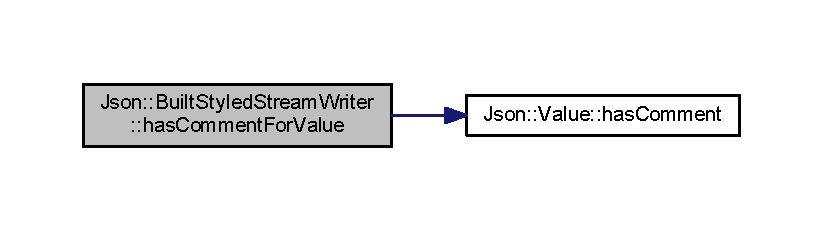
\includegraphics[width=350pt]{struct_json_1_1_built_styled_stream_writer_a457c2f3c1e8c952caeb60e52477d0c9a_cgraph}
\end{center}
\end{figure}
이 함수를 호출하는 함수들에 대한 그래프입니다.\+:\nopagebreak
\begin{figure}[H]
\begin{center}
\leavevmode
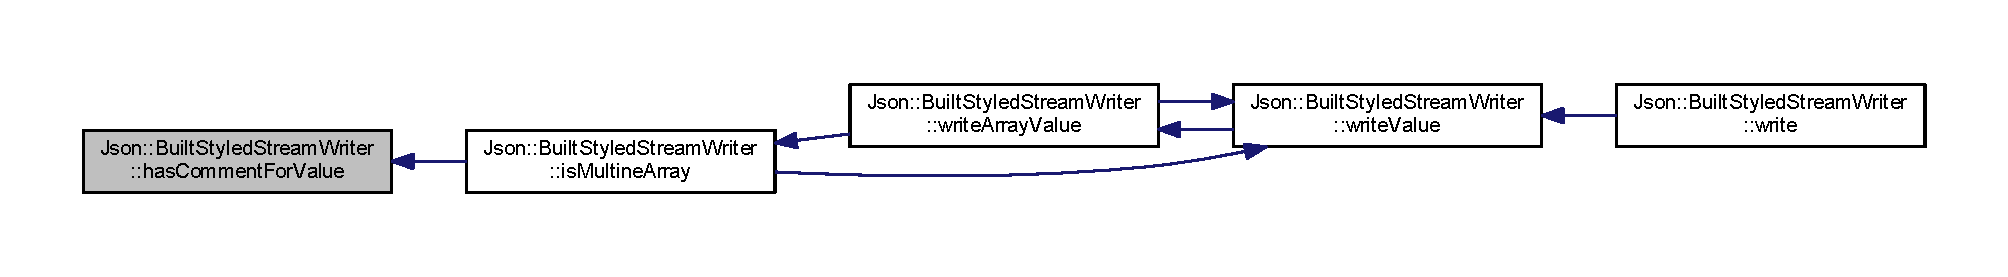
\includegraphics[width=350pt]{struct_json_1_1_built_styled_stream_writer_a457c2f3c1e8c952caeb60e52477d0c9a_icgraph}
\end{center}
\end{figure}
\mbox{\Hypertarget{struct_json_1_1_built_styled_stream_writer_a73e09692a2cfbd6e67836b060dc34a9f}\label{struct_json_1_1_built_styled_stream_writer_a73e09692a2cfbd6e67836b060dc34a9f}} 
\index{Json\+::\+Built\+Styled\+Stream\+Writer@{Json\+::\+Built\+Styled\+Stream\+Writer}!indent@{indent}}
\index{indent@{indent}!Json\+::\+Built\+Styled\+Stream\+Writer@{Json\+::\+Built\+Styled\+Stream\+Writer}}
\subsubsection{\texorpdfstring{indent()}{indent()}}
{\footnotesize\ttfamily void Json\+::\+Built\+Styled\+Stream\+Writer\+::indent (\begin{DoxyParamCaption}{ }\end{DoxyParamCaption})\hspace{0.3cm}{\ttfamily [private]}}



jsoncpp.\+cpp 파일의 5151 번째 라인에서 정의되었습니다.


\begin{DoxyCode}
5151 \{ \hyperlink{struct_json_1_1_built_styled_stream_writer_a0f8115a4fb474ab0e9de25f10e5ca09a}{indentString\_} += \hyperlink{struct_json_1_1_built_styled_stream_writer_aaa4cbad91428ceca37cbabfc2a17a92d}{indentation\_}; \}
\end{DoxyCode}
이 함수를 호출하는 함수들에 대한 그래프입니다.\+:\nopagebreak
\begin{figure}[H]
\begin{center}
\leavevmode
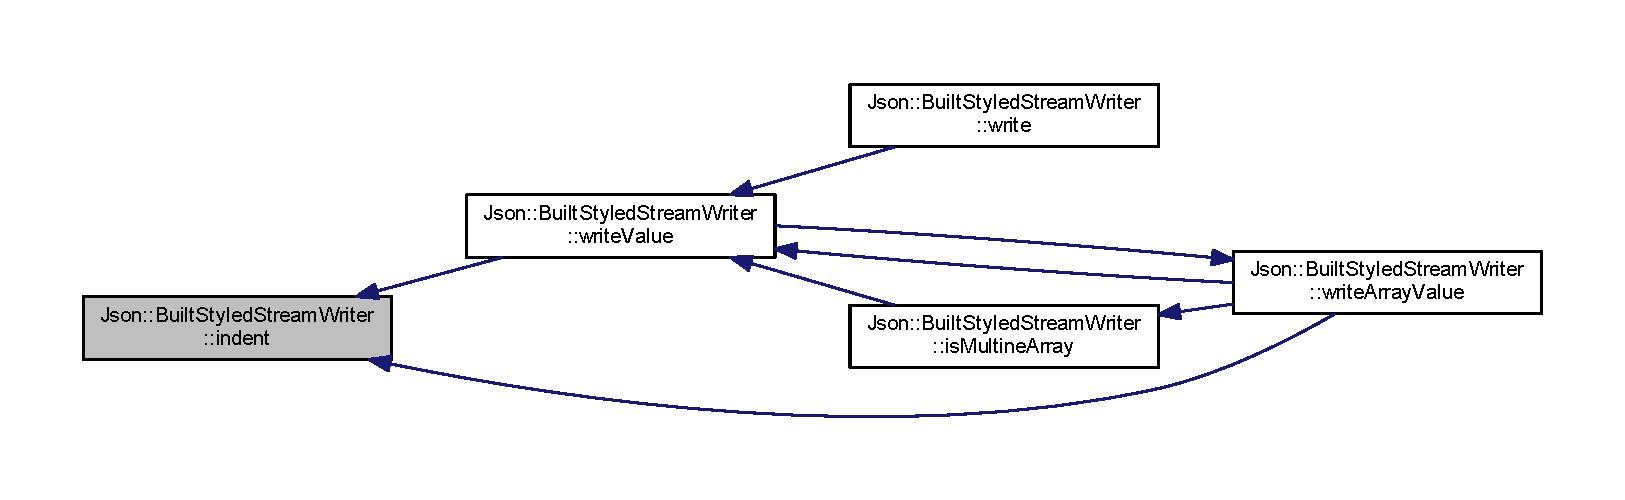
\includegraphics[width=350pt]{struct_json_1_1_built_styled_stream_writer_a73e09692a2cfbd6e67836b060dc34a9f_icgraph}
\end{center}
\end{figure}
\mbox{\Hypertarget{struct_json_1_1_built_styled_stream_writer_af423fd33b3d580506ea3efc53b05a077}\label{struct_json_1_1_built_styled_stream_writer_af423fd33b3d580506ea3efc53b05a077}} 
\index{Json\+::\+Built\+Styled\+Stream\+Writer@{Json\+::\+Built\+Styled\+Stream\+Writer}!is\+Multine\+Array@{is\+Multine\+Array}}
\index{is\+Multine\+Array@{is\+Multine\+Array}!Json\+::\+Built\+Styled\+Stream\+Writer@{Json\+::\+Built\+Styled\+Stream\+Writer}}
\subsubsection{\texorpdfstring{is\+Multine\+Array()}{isMultineArray()}}
{\footnotesize\ttfamily bool Json\+::\+Built\+Styled\+Stream\+Writer\+::is\+Multine\+Array (\begin{DoxyParamCaption}\item[{\hyperlink{class_json_1_1_value}{Value} const \&}]{value }\end{DoxyParamCaption})\hspace{0.3cm}{\ttfamily [private]}}



jsoncpp.\+cpp 파일의 5099 번째 라인에서 정의되었습니다.


\begin{DoxyCode}
5099                                                                \{
5100   \hyperlink{namespace_json_a8048e741f2177c3b5d9ede4a5b8c53c2}{ArrayIndex} \textcolor{keyword}{const} size = value.size();
5101   \textcolor{keywordtype}{bool} isMultiLine = size * 3 >= \hyperlink{struct_json_1_1_built_styled_stream_writer_a06a51521ccae20397f52fe3036edc602}{rightMargin\_};
5102   \hyperlink{struct_json_1_1_built_styled_stream_writer_a47d562d7874c5b1e68995bd62f575792}{childValues\_}.clear();
5103   \textcolor{keywordflow}{for} (\hyperlink{namespace_json_a8048e741f2177c3b5d9ede4a5b8c53c2}{ArrayIndex} index = 0; index < size && !isMultiLine; ++index) \{
5104     \hyperlink{class_json_1_1_value}{Value} \textcolor{keyword}{const}& childValue = value[index];
5105     isMultiLine = ((childValue.\hyperlink{class_json_1_1_value_a1627eb9d6568d6d0252fa8bb711c0a59}{isArray}() || childValue.\hyperlink{class_json_1_1_value_a8cf96c0f2a552051fcfc78ffee60e037}{isObject}()) &&
5106                         childValue.\hyperlink{class_json_1_1_value_a0ec2808e1d7efa4e9fad938d6667be44}{size}() > 0);
5107   \}
5108   \textcolor{keywordflow}{if} (!isMultiLine) \textcolor{comment}{// check if line length > max line length}
5109   \{
5110     \hyperlink{struct_json_1_1_built_styled_stream_writer_a47d562d7874c5b1e68995bd62f575792}{childValues\_}.reserve(size);
5111     \hyperlink{struct_json_1_1_built_styled_stream_writer_abed9cc31da503b48798e7cea68c42e16}{addChildValues\_} = \textcolor{keyword}{true};
5112     \hyperlink{namespace_json_a8048e741f2177c3b5d9ede4a5b8c53c2}{ArrayIndex} lineLength = 4 + (size - 1) * 2; \textcolor{comment}{// '[ ' + ', '*n + ' ]'}
5113     \textcolor{keywordflow}{for} (\hyperlink{namespace_json_a8048e741f2177c3b5d9ede4a5b8c53c2}{ArrayIndex} index = 0; index < size; ++index) \{
5114       \textcolor{keywordflow}{if} (\hyperlink{struct_json_1_1_built_styled_stream_writer_a457c2f3c1e8c952caeb60e52477d0c9a}{hasCommentForValue}(value[index])) \{
5115         isMultiLine = \textcolor{keyword}{true};
5116       \}
5117       \hyperlink{struct_json_1_1_built_styled_stream_writer_a7c9da861861e570a51b45f270c9ff150}{writeValue}(value[index]);
5118       lineLength += \textcolor{keyword}{static\_cast<}\hyperlink{namespace_json_a8048e741f2177c3b5d9ede4a5b8c53c2}{ArrayIndex}\textcolor{keyword}{>}(\hyperlink{struct_json_1_1_built_styled_stream_writer_a47d562d7874c5b1e68995bd62f575792}{childValues\_}[index].length());
5119     \}
5120     \hyperlink{struct_json_1_1_built_styled_stream_writer_abed9cc31da503b48798e7cea68c42e16}{addChildValues\_} = \textcolor{keyword}{false};
5121     isMultiLine = isMultiLine || lineLength >= \hyperlink{struct_json_1_1_built_styled_stream_writer_a06a51521ccae20397f52fe3036edc602}{rightMargin\_};
5122   \}
5123   \textcolor{keywordflow}{return} isMultiLine;
5124 \}
\end{DoxyCode}
이 함수 내부에서 호출하는 함수들에 대한 그래프입니다.\+:
\nopagebreak
\begin{figure}[H]
\begin{center}
\leavevmode
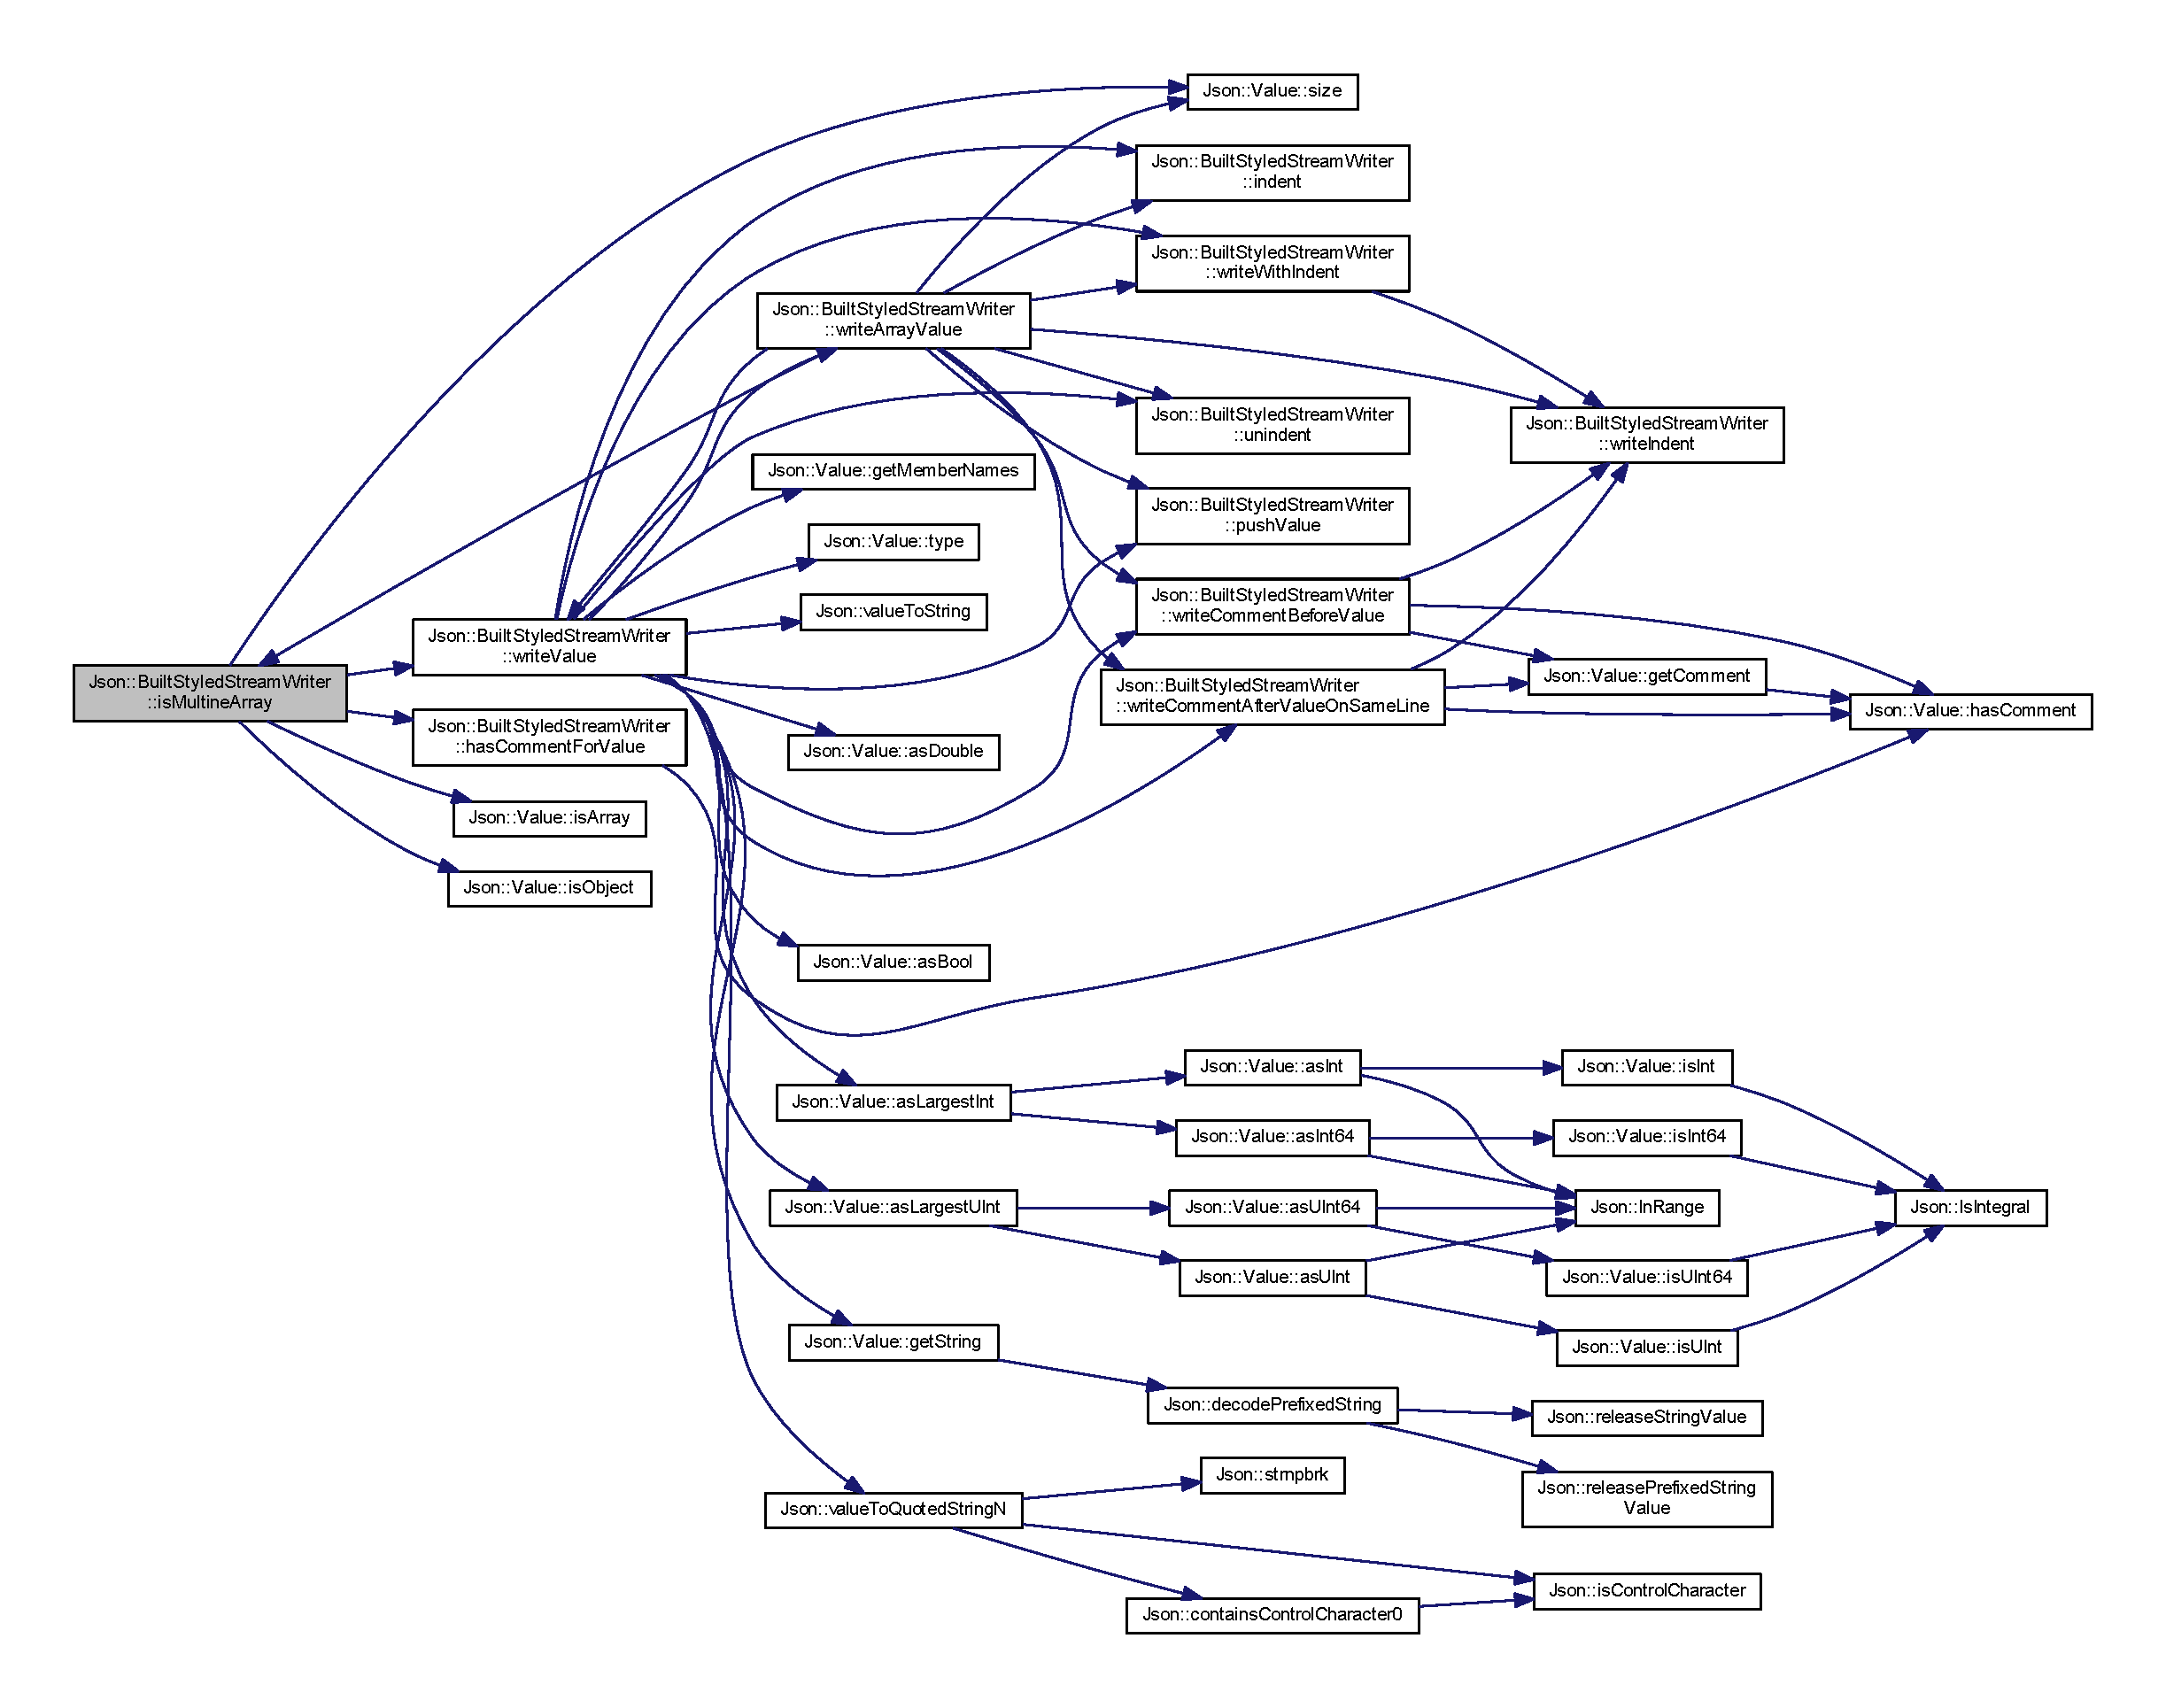
\includegraphics[width=350pt]{struct_json_1_1_built_styled_stream_writer_af423fd33b3d580506ea3efc53b05a077_cgraph}
\end{center}
\end{figure}
이 함수를 호출하는 함수들에 대한 그래프입니다.\+:\nopagebreak
\begin{figure}[H]
\begin{center}
\leavevmode
\includegraphics[width=350pt]{struct_json_1_1_built_styled_stream_writer_af423fd33b3d580506ea3efc53b05a077_icgraph}
\end{center}
\end{figure}
\mbox{\Hypertarget{struct_json_1_1_built_styled_stream_writer_a91e8535508412eea04d77c0cafdf15aa}\label{struct_json_1_1_built_styled_stream_writer_a91e8535508412eea04d77c0cafdf15aa}} 
\index{Json\+::\+Built\+Styled\+Stream\+Writer@{Json\+::\+Built\+Styled\+Stream\+Writer}!push\+Value@{push\+Value}}
\index{push\+Value@{push\+Value}!Json\+::\+Built\+Styled\+Stream\+Writer@{Json\+::\+Built\+Styled\+Stream\+Writer}}
\subsubsection{\texorpdfstring{push\+Value()}{pushValue()}}
{\footnotesize\ttfamily void Json\+::\+Built\+Styled\+Stream\+Writer\+::push\+Value (\begin{DoxyParamCaption}\item[{\hyperlink{json_8h_a1e723f95759de062585bc4a8fd3fa4be}{J\+S\+O\+N\+C\+P\+P\+\_\+\+S\+T\+R\+I\+NG} const \&}]{value }\end{DoxyParamCaption})\hspace{0.3cm}{\ttfamily [private]}}



jsoncpp.\+cpp 파일의 5126 번째 라인에서 정의되었습니다.


\begin{DoxyCode}
5126                                                                    \{
5127   \textcolor{keywordflow}{if} (\hyperlink{struct_json_1_1_built_styled_stream_writer_abed9cc31da503b48798e7cea68c42e16}{addChildValues\_})
5128     \hyperlink{struct_json_1_1_built_styled_stream_writer_a47d562d7874c5b1e68995bd62f575792}{childValues\_}.push\_back(value);
5129   \textcolor{keywordflow}{else}
5130     *\hyperlink{class_json_1_1_stream_writer_a4f5603d4228a9fa46a42cb44e5234d9b}{sout\_} << value;
5131 \}
\end{DoxyCode}
이 함수를 호출하는 함수들에 대한 그래프입니다.\+:\nopagebreak
\begin{figure}[H]
\begin{center}
\leavevmode
\includegraphics[width=350pt]{struct_json_1_1_built_styled_stream_writer_a91e8535508412eea04d77c0cafdf15aa_icgraph}
\end{center}
\end{figure}
\mbox{\Hypertarget{struct_json_1_1_built_styled_stream_writer_a0da6c6f603e00c8c6e38af553edd8c55}\label{struct_json_1_1_built_styled_stream_writer_a0da6c6f603e00c8c6e38af553edd8c55}} 
\index{Json\+::\+Built\+Styled\+Stream\+Writer@{Json\+::\+Built\+Styled\+Stream\+Writer}!unindent@{unindent}}
\index{unindent@{unindent}!Json\+::\+Built\+Styled\+Stream\+Writer@{Json\+::\+Built\+Styled\+Stream\+Writer}}
\subsubsection{\texorpdfstring{unindent()}{unindent()}}
{\footnotesize\ttfamily void Json\+::\+Built\+Styled\+Stream\+Writer\+::unindent (\begin{DoxyParamCaption}{ }\end{DoxyParamCaption})\hspace{0.3cm}{\ttfamily [private]}}



jsoncpp.\+cpp 파일의 5153 번째 라인에서 정의되었습니다.


\begin{DoxyCode}
5153                                        \{
5154   assert(\hyperlink{struct_json_1_1_built_styled_stream_writer_a0f8115a4fb474ab0e9de25f10e5ca09a}{indentString\_}.size() >= \hyperlink{struct_json_1_1_built_styled_stream_writer_aaa4cbad91428ceca37cbabfc2a17a92d}{indentation\_}.size());
5155   \hyperlink{struct_json_1_1_built_styled_stream_writer_a0f8115a4fb474ab0e9de25f10e5ca09a}{indentString\_}.resize(\hyperlink{struct_json_1_1_built_styled_stream_writer_a0f8115a4fb474ab0e9de25f10e5ca09a}{indentString\_}.size() - 
      \hyperlink{struct_json_1_1_built_styled_stream_writer_aaa4cbad91428ceca37cbabfc2a17a92d}{indentation\_}.size());
5156 \}
\end{DoxyCode}
이 함수를 호출하는 함수들에 대한 그래프입니다.\+:\nopagebreak
\begin{figure}[H]
\begin{center}
\leavevmode
\includegraphics[width=350pt]{struct_json_1_1_built_styled_stream_writer_a0da6c6f603e00c8c6e38af553edd8c55_icgraph}
\end{center}
\end{figure}
\mbox{\Hypertarget{struct_json_1_1_built_styled_stream_writer_a823cdb1afabb6b0d5f39bcd5a6a6f747}\label{struct_json_1_1_built_styled_stream_writer_a823cdb1afabb6b0d5f39bcd5a6a6f747}} 
\index{Json\+::\+Built\+Styled\+Stream\+Writer@{Json\+::\+Built\+Styled\+Stream\+Writer}!write@{write}}
\index{write@{write}!Json\+::\+Built\+Styled\+Stream\+Writer@{Json\+::\+Built\+Styled\+Stream\+Writer}}
\subsubsection{\texorpdfstring{write()}{write()}}
{\footnotesize\ttfamily int Json\+::\+Built\+Styled\+Stream\+Writer\+::write (\begin{DoxyParamCaption}\item[{\hyperlink{class_json_1_1_value}{Value} const \&}]{root,  }\item[{\hyperlink{json_8h_a37a25be5fca174927780caeb280094ce}{J\+S\+O\+N\+C\+P\+P\+\_\+\+O\+S\+T\+R\+E\+AM} $\ast$}]{sout }\end{DoxyParamCaption})\hspace{0.3cm}{\ttfamily [virtual]}}

Write \hyperlink{class_json_1_1_value}{Value} into document as configured in sub-\/class. Do not take ownership of sout, but maintain a reference during function. \begin{DoxyPrecond}{전제조건}
sout != N\+U\+LL 
\end{DoxyPrecond}
\begin{DoxyReturn}{반환값}
zero on success (For now, we always return zero, so check the stream instead.) 
\end{DoxyReturn}

\begin{DoxyExceptions}{예외}
{\em std\+::exception} & possibly, depending on configuration \\
\hline
\end{DoxyExceptions}


\hyperlink{class_json_1_1_stream_writer_a84278bad0c9a9fc587bc2a97c5bb5993}{Json\+::\+Stream\+Writer}를 구현.



jsoncpp.\+cpp 파일의 4978 번째 라인에서 정의되었습니다.


\begin{DoxyCode}
4979 \{
4980   \hyperlink{class_json_1_1_stream_writer_a4f5603d4228a9fa46a42cb44e5234d9b}{sout\_} = sout;
4981   \hyperlink{struct_json_1_1_built_styled_stream_writer_abed9cc31da503b48798e7cea68c42e16}{addChildValues\_} = \textcolor{keyword}{false};
4982   \hyperlink{struct_json_1_1_built_styled_stream_writer_a6aa0ad023e623f600103631a6bca6d10}{indented\_} = \textcolor{keyword}{true};
4983   \hyperlink{struct_json_1_1_built_styled_stream_writer_a0f8115a4fb474ab0e9de25f10e5ca09a}{indentString\_} = \textcolor{stringliteral}{""};
4984   \hyperlink{struct_json_1_1_built_styled_stream_writer_a32c4afca4e08fba79bb0a80a8010283a}{writeCommentBeforeValue}(root);
4985   \textcolor{keywordflow}{if} (!\hyperlink{struct_json_1_1_built_styled_stream_writer_a6aa0ad023e623f600103631a6bca6d10}{indented\_}) \hyperlink{struct_json_1_1_built_styled_stream_writer_a2b38a3714d415c4bd3b4812897130f3d}{writeIndent}();
4986   \hyperlink{struct_json_1_1_built_styled_stream_writer_a6aa0ad023e623f600103631a6bca6d10}{indented\_} = \textcolor{keyword}{true};
4987   \hyperlink{struct_json_1_1_built_styled_stream_writer_a7c9da861861e570a51b45f270c9ff150}{writeValue}(root);
4988   \hyperlink{struct_json_1_1_built_styled_stream_writer_a89625b134fce0255263ca40e6125742b}{writeCommentAfterValueOnSameLine}(root);
4989   *\hyperlink{class_json_1_1_stream_writer_a4f5603d4228a9fa46a42cb44e5234d9b}{sout\_} << \hyperlink{struct_json_1_1_built_styled_stream_writer_a5e61a9a4b2af52b98900286c843b86f7}{endingLineFeedSymbol\_};
4990   \hyperlink{class_json_1_1_stream_writer_a4f5603d4228a9fa46a42cb44e5234d9b}{sout\_} = NULL;
4991   \textcolor{keywordflow}{return} 0;
4992 \}
\end{DoxyCode}
이 함수 내부에서 호출하는 함수들에 대한 그래프입니다.\+:
\nopagebreak
\begin{figure}[H]
\begin{center}
\leavevmode
\includegraphics[width=350pt]{struct_json_1_1_built_styled_stream_writer_a823cdb1afabb6b0d5f39bcd5a6a6f747_cgraph}
\end{center}
\end{figure}
\mbox{\Hypertarget{struct_json_1_1_built_styled_stream_writer_acd20e9274bbcf7876ef3af2e7d23a31f}\label{struct_json_1_1_built_styled_stream_writer_acd20e9274bbcf7876ef3af2e7d23a31f}} 
\index{Json\+::\+Built\+Styled\+Stream\+Writer@{Json\+::\+Built\+Styled\+Stream\+Writer}!write\+Array\+Value@{write\+Array\+Value}}
\index{write\+Array\+Value@{write\+Array\+Value}!Json\+::\+Built\+Styled\+Stream\+Writer@{Json\+::\+Built\+Styled\+Stream\+Writer}}
\subsubsection{\texorpdfstring{write\+Array\+Value()}{writeArrayValue()}}
{\footnotesize\ttfamily void Json\+::\+Built\+Styled\+Stream\+Writer\+::write\+Array\+Value (\begin{DoxyParamCaption}\item[{\hyperlink{class_json_1_1_value}{Value} const \&}]{value }\end{DoxyParamCaption})\hspace{0.3cm}{\ttfamily [private]}}



jsoncpp.\+cpp 파일의 5052 번째 라인에서 정의되었습니다.


\begin{DoxyCode}
5052                                                                 \{
5053   \textcolor{keywordtype}{unsigned} size = value.size();
5054   \textcolor{keywordflow}{if} (size == 0)
5055     \hyperlink{struct_json_1_1_built_styled_stream_writer_a91e8535508412eea04d77c0cafdf15aa}{pushValue}(\textcolor{stringliteral}{"[]"});
5056   \textcolor{keywordflow}{else} \{
5057     \textcolor{keywordtype}{bool} isMultiLine = (\hyperlink{struct_json_1_1_built_styled_stream_writer_a89a9c76c7531143b52785861ba21c1d4}{cs\_} == \hyperlink{struct_json_1_1_comment_style_a51fc08f3518fd81eba12f340d19a3d0ca32302c0b97190c1808b3e38f367fef01}{CommentStyle::All}) || 
      \hyperlink{struct_json_1_1_built_styled_stream_writer_af423fd33b3d580506ea3efc53b05a077}{isMultineArray}(value);
5058     \textcolor{keywordflow}{if} (isMultiLine) \{
5059       \hyperlink{struct_json_1_1_built_styled_stream_writer_a6e80e1a0d5f64df2ec48c3c3b1284990}{writeWithIndent}(\textcolor{stringliteral}{"["});
5060       \hyperlink{struct_json_1_1_built_styled_stream_writer_a73e09692a2cfbd6e67836b060dc34a9f}{indent}();
5061       \textcolor{keywordtype}{bool} hasChildValue = !\hyperlink{struct_json_1_1_built_styled_stream_writer_a47d562d7874c5b1e68995bd62f575792}{childValues\_}.empty();
5062       \textcolor{keywordtype}{unsigned} index = 0;
5063       \textcolor{keywordflow}{for} (;;) \{
5064         \hyperlink{class_json_1_1_value}{Value} \textcolor{keyword}{const}& childValue = value[index];
5065         \hyperlink{struct_json_1_1_built_styled_stream_writer_a32c4afca4e08fba79bb0a80a8010283a}{writeCommentBeforeValue}(childValue);
5066         \textcolor{keywordflow}{if} (hasChildValue)
5067           \hyperlink{struct_json_1_1_built_styled_stream_writer_a6e80e1a0d5f64df2ec48c3c3b1284990}{writeWithIndent}(\hyperlink{struct_json_1_1_built_styled_stream_writer_a47d562d7874c5b1e68995bd62f575792}{childValues\_}[index]);
5068         \textcolor{keywordflow}{else} \{
5069           \textcolor{keywordflow}{if} (!\hyperlink{struct_json_1_1_built_styled_stream_writer_a6aa0ad023e623f600103631a6bca6d10}{indented\_}) \hyperlink{struct_json_1_1_built_styled_stream_writer_a2b38a3714d415c4bd3b4812897130f3d}{writeIndent}();
5070           \hyperlink{struct_json_1_1_built_styled_stream_writer_a6aa0ad023e623f600103631a6bca6d10}{indented\_} = \textcolor{keyword}{true};
5071           \hyperlink{struct_json_1_1_built_styled_stream_writer_a7c9da861861e570a51b45f270c9ff150}{writeValue}(childValue);
5072           \hyperlink{struct_json_1_1_built_styled_stream_writer_a6aa0ad023e623f600103631a6bca6d10}{indented\_} = \textcolor{keyword}{false};
5073         \}
5074         \textcolor{keywordflow}{if} (++index == size) \{
5075           \hyperlink{struct_json_1_1_built_styled_stream_writer_a89625b134fce0255263ca40e6125742b}{writeCommentAfterValueOnSameLine}(childValue);
5076           \textcolor{keywordflow}{break};
5077         \}
5078         *\hyperlink{class_json_1_1_stream_writer_a4f5603d4228a9fa46a42cb44e5234d9b}{sout\_} << \textcolor{stringliteral}{","};
5079         \hyperlink{struct_json_1_1_built_styled_stream_writer_a89625b134fce0255263ca40e6125742b}{writeCommentAfterValueOnSameLine}(childValue);
5080       \}
5081       \hyperlink{struct_json_1_1_built_styled_stream_writer_a0da6c6f603e00c8c6e38af553edd8c55}{unindent}();
5082       \hyperlink{struct_json_1_1_built_styled_stream_writer_a6e80e1a0d5f64df2ec48c3c3b1284990}{writeWithIndent}(\textcolor{stringliteral}{"]"});
5083     \} \textcolor{keywordflow}{else} \textcolor{comment}{// output on a single line}
5084     \{
5085       assert(\hyperlink{struct_json_1_1_built_styled_stream_writer_a47d562d7874c5b1e68995bd62f575792}{childValues\_}.size() == size);
5086       *\hyperlink{class_json_1_1_stream_writer_a4f5603d4228a9fa46a42cb44e5234d9b}{sout\_} << \textcolor{stringliteral}{"["};
5087       \textcolor{keywordflow}{if} (!\hyperlink{struct_json_1_1_built_styled_stream_writer_aaa4cbad91428ceca37cbabfc2a17a92d}{indentation\_}.empty()) *sout\_ << \textcolor{stringliteral}{" "};
5088       \textcolor{keywordflow}{for} (\textcolor{keywordtype}{unsigned} index = 0; index < size; ++index) \{
5089         \textcolor{keywordflow}{if} (index > 0)
5090           *sout\_ << ((!\hyperlink{struct_json_1_1_built_styled_stream_writer_aaa4cbad91428ceca37cbabfc2a17a92d}{indentation\_}.empty()) ? \textcolor{stringliteral}{", "} : \textcolor{stringliteral}{","});
5091         *sout\_ << \hyperlink{struct_json_1_1_built_styled_stream_writer_a47d562d7874c5b1e68995bd62f575792}{childValues\_}[index];
5092       \}
5093       \textcolor{keywordflow}{if} (!\hyperlink{struct_json_1_1_built_styled_stream_writer_aaa4cbad91428ceca37cbabfc2a17a92d}{indentation\_}.empty()) *sout\_ << \textcolor{stringliteral}{" "};
5094       *sout\_ << \textcolor{stringliteral}{"]"};
5095     \}
5096   \}
5097 \}
\end{DoxyCode}
이 함수 내부에서 호출하는 함수들에 대한 그래프입니다.\+:
\nopagebreak
\begin{figure}[H]
\begin{center}
\leavevmode
\includegraphics[width=350pt]{struct_json_1_1_built_styled_stream_writer_acd20e9274bbcf7876ef3af2e7d23a31f_cgraph}
\end{center}
\end{figure}
이 함수를 호출하는 함수들에 대한 그래프입니다.\+:\nopagebreak
\begin{figure}[H]
\begin{center}
\leavevmode
\includegraphics[width=350pt]{struct_json_1_1_built_styled_stream_writer_acd20e9274bbcf7876ef3af2e7d23a31f_icgraph}
\end{center}
\end{figure}
\mbox{\Hypertarget{struct_json_1_1_built_styled_stream_writer_a89625b134fce0255263ca40e6125742b}\label{struct_json_1_1_built_styled_stream_writer_a89625b134fce0255263ca40e6125742b}} 
\index{Json\+::\+Built\+Styled\+Stream\+Writer@{Json\+::\+Built\+Styled\+Stream\+Writer}!write\+Comment\+After\+Value\+On\+Same\+Line@{write\+Comment\+After\+Value\+On\+Same\+Line}}
\index{write\+Comment\+After\+Value\+On\+Same\+Line@{write\+Comment\+After\+Value\+On\+Same\+Line}!Json\+::\+Built\+Styled\+Stream\+Writer@{Json\+::\+Built\+Styled\+Stream\+Writer}}
\subsubsection{\texorpdfstring{write\+Comment\+After\+Value\+On\+Same\+Line()}{writeCommentAfterValueOnSameLine()}}
{\footnotesize\ttfamily void Json\+::\+Built\+Styled\+Stream\+Writer\+::write\+Comment\+After\+Value\+On\+Same\+Line (\begin{DoxyParamCaption}\item[{\hyperlink{class_json_1_1_value}{Value} const \&}]{root }\end{DoxyParamCaption})\hspace{0.3cm}{\ttfamily [private]}}



jsoncpp.\+cpp 파일의 5177 번째 라인에서 정의되었습니다.


\begin{DoxyCode}
5177                                                                                 \{
5178   \textcolor{keywordflow}{if} (\hyperlink{struct_json_1_1_built_styled_stream_writer_a89a9c76c7531143b52785861ba21c1d4}{cs\_} == \hyperlink{struct_json_1_1_comment_style_a51fc08f3518fd81eba12f340d19a3d0cac8b32a8bae63414c8647d4919da8d437}{CommentStyle::None}) \textcolor{keywordflow}{return};
5179   \textcolor{keywordflow}{if} (root.hasComment(\hyperlink{namespace_json_a4fc417c23905b2ae9e2c47d197a45351a008a230a0586de54f30b76afe70fdcfa}{commentAfterOnSameLine}))
5180     *\hyperlink{class_json_1_1_stream_writer_a4f5603d4228a9fa46a42cb44e5234d9b}{sout\_} << \textcolor{stringliteral}{" "} + root.getComment(\hyperlink{namespace_json_a4fc417c23905b2ae9e2c47d197a45351a008a230a0586de54f30b76afe70fdcfa}{commentAfterOnSameLine});
5181 
5182   \textcolor{keywordflow}{if} (root.hasComment(\hyperlink{namespace_json_a4fc417c23905b2ae9e2c47d197a45351ac5784ca53b12250888ddb642b06aebef}{commentAfter})) \{
5183     \hyperlink{struct_json_1_1_built_styled_stream_writer_a2b38a3714d415c4bd3b4812897130f3d}{writeIndent}();
5184     *\hyperlink{class_json_1_1_stream_writer_a4f5603d4228a9fa46a42cb44e5234d9b}{sout\_} << root.getComment(\hyperlink{namespace_json_a4fc417c23905b2ae9e2c47d197a45351ac5784ca53b12250888ddb642b06aebef}{commentAfter});
5185   \}
5186 \}
\end{DoxyCode}
이 함수 내부에서 호출하는 함수들에 대한 그래프입니다.\+:\nopagebreak
\begin{figure}[H]
\begin{center}
\leavevmode
\includegraphics[width=350pt]{struct_json_1_1_built_styled_stream_writer_a89625b134fce0255263ca40e6125742b_cgraph}
\end{center}
\end{figure}
이 함수를 호출하는 함수들에 대한 그래프입니다.\+:\nopagebreak
\begin{figure}[H]
\begin{center}
\leavevmode
\includegraphics[width=350pt]{struct_json_1_1_built_styled_stream_writer_a89625b134fce0255263ca40e6125742b_icgraph}
\end{center}
\end{figure}
\mbox{\Hypertarget{struct_json_1_1_built_styled_stream_writer_a32c4afca4e08fba79bb0a80a8010283a}\label{struct_json_1_1_built_styled_stream_writer_a32c4afca4e08fba79bb0a80a8010283a}} 
\index{Json\+::\+Built\+Styled\+Stream\+Writer@{Json\+::\+Built\+Styled\+Stream\+Writer}!write\+Comment\+Before\+Value@{write\+Comment\+Before\+Value}}
\index{write\+Comment\+Before\+Value@{write\+Comment\+Before\+Value}!Json\+::\+Built\+Styled\+Stream\+Writer@{Json\+::\+Built\+Styled\+Stream\+Writer}}
\subsubsection{\texorpdfstring{write\+Comment\+Before\+Value()}{writeCommentBeforeValue()}}
{\footnotesize\ttfamily void Json\+::\+Built\+Styled\+Stream\+Writer\+::write\+Comment\+Before\+Value (\begin{DoxyParamCaption}\item[{\hyperlink{class_json_1_1_value}{Value} const \&}]{root }\end{DoxyParamCaption})\hspace{0.3cm}{\ttfamily [private]}}



jsoncpp.\+cpp 파일의 5158 번째 라인에서 정의되었습니다.


\begin{DoxyCode}
5158                                                                        \{
5159   \textcolor{keywordflow}{if} (\hyperlink{struct_json_1_1_built_styled_stream_writer_a89a9c76c7531143b52785861ba21c1d4}{cs\_} == \hyperlink{struct_json_1_1_comment_style_a51fc08f3518fd81eba12f340d19a3d0cac8b32a8bae63414c8647d4919da8d437}{CommentStyle::None}) \textcolor{keywordflow}{return};
5160   \textcolor{keywordflow}{if} (!root.hasComment(\hyperlink{namespace_json_a4fc417c23905b2ae9e2c47d197a45351a52f1733775460517b2ea6bedf4906d52}{commentBefore}))
5161     \textcolor{keywordflow}{return};
5162 
5163   \textcolor{keywordflow}{if} (!\hyperlink{struct_json_1_1_built_styled_stream_writer_a6aa0ad023e623f600103631a6bca6d10}{indented\_}) \hyperlink{struct_json_1_1_built_styled_stream_writer_a2b38a3714d415c4bd3b4812897130f3d}{writeIndent}();
5164   \textcolor{keyword}{const} \hyperlink{json-forwards_8h_a1e723f95759de062585bc4a8fd3fa4be}{JSONCPP\_STRING}& comment = root.getComment(\hyperlink{namespace_json_a4fc417c23905b2ae9e2c47d197a45351a52f1733775460517b2ea6bedf4906d52}{commentBefore});
5165   JSONCPP\_STRING::const\_iterator iter = comment.begin();
5166   \textcolor{keywordflow}{while} (iter != comment.end()) \{
5167     *\hyperlink{class_json_1_1_stream_writer_a4f5603d4228a9fa46a42cb44e5234d9b}{sout\_} << *iter;
5168     \textcolor{keywordflow}{if} (*iter == \textcolor{charliteral}{'\(\backslash\)n'} &&
5169        (iter != comment.end() && *(iter + 1) == \textcolor{charliteral}{'/'}))
5170       \textcolor{comment}{// writeIndent();  // would write extra newline}
5171       *\hyperlink{class_json_1_1_stream_writer_a4f5603d4228a9fa46a42cb44e5234d9b}{sout\_} << \hyperlink{struct_json_1_1_built_styled_stream_writer_a0f8115a4fb474ab0e9de25f10e5ca09a}{indentString\_};
5172     ++iter;
5173   \}
5174   \hyperlink{struct_json_1_1_built_styled_stream_writer_a6aa0ad023e623f600103631a6bca6d10}{indented\_} = \textcolor{keyword}{false};
5175 \}
\end{DoxyCode}
이 함수 내부에서 호출하는 함수들에 대한 그래프입니다.\+:\nopagebreak
\begin{figure}[H]
\begin{center}
\leavevmode
\includegraphics[width=350pt]{struct_json_1_1_built_styled_stream_writer_a32c4afca4e08fba79bb0a80a8010283a_cgraph}
\end{center}
\end{figure}
이 함수를 호출하는 함수들에 대한 그래프입니다.\+:\nopagebreak
\begin{figure}[H]
\begin{center}
\leavevmode
\includegraphics[width=350pt]{struct_json_1_1_built_styled_stream_writer_a32c4afca4e08fba79bb0a80a8010283a_icgraph}
\end{center}
\end{figure}
\mbox{\Hypertarget{struct_json_1_1_built_styled_stream_writer_a2b38a3714d415c4bd3b4812897130f3d}\label{struct_json_1_1_built_styled_stream_writer_a2b38a3714d415c4bd3b4812897130f3d}} 
\index{Json\+::\+Built\+Styled\+Stream\+Writer@{Json\+::\+Built\+Styled\+Stream\+Writer}!write\+Indent@{write\+Indent}}
\index{write\+Indent@{write\+Indent}!Json\+::\+Built\+Styled\+Stream\+Writer@{Json\+::\+Built\+Styled\+Stream\+Writer}}
\subsubsection{\texorpdfstring{write\+Indent()}{writeIndent()}}
{\footnotesize\ttfamily void Json\+::\+Built\+Styled\+Stream\+Writer\+::write\+Indent (\begin{DoxyParamCaption}{ }\end{DoxyParamCaption})\hspace{0.3cm}{\ttfamily [private]}}



jsoncpp.\+cpp 파일의 5133 번째 라인에서 정의되었습니다.


\begin{DoxyCode}
5133                                           \{
5134   \textcolor{comment}{// blep intended this to look at the so-far-written string}
5135   \textcolor{comment}{// to determine whether we are already indented, but}
5136   \textcolor{comment}{// with a stream we cannot do that. So we rely on some saved state.}
5137   \textcolor{comment}{// The caller checks indented\_.}
5138 
5139   \textcolor{keywordflow}{if} (!\hyperlink{struct_json_1_1_built_styled_stream_writer_aaa4cbad91428ceca37cbabfc2a17a92d}{indentation\_}.empty()) \{
5140     \textcolor{comment}{// In this case, drop newlines too.}
5141     *\hyperlink{class_json_1_1_stream_writer_a4f5603d4228a9fa46a42cb44e5234d9b}{sout\_} << \textcolor{charliteral}{'\(\backslash\)n'} << \hyperlink{struct_json_1_1_built_styled_stream_writer_a0f8115a4fb474ab0e9de25f10e5ca09a}{indentString\_};
5142   \}
5143 \}
\end{DoxyCode}
이 함수를 호출하는 함수들에 대한 그래프입니다.\+:\nopagebreak
\begin{figure}[H]
\begin{center}
\leavevmode
\includegraphics[width=350pt]{struct_json_1_1_built_styled_stream_writer_a2b38a3714d415c4bd3b4812897130f3d_icgraph}
\end{center}
\end{figure}
\mbox{\Hypertarget{struct_json_1_1_built_styled_stream_writer_a7c9da861861e570a51b45f270c9ff150}\label{struct_json_1_1_built_styled_stream_writer_a7c9da861861e570a51b45f270c9ff150}} 
\index{Json\+::\+Built\+Styled\+Stream\+Writer@{Json\+::\+Built\+Styled\+Stream\+Writer}!write\+Value@{write\+Value}}
\index{write\+Value@{write\+Value}!Json\+::\+Built\+Styled\+Stream\+Writer@{Json\+::\+Built\+Styled\+Stream\+Writer}}
\subsubsection{\texorpdfstring{write\+Value()}{writeValue()}}
{\footnotesize\ttfamily void Json\+::\+Built\+Styled\+Stream\+Writer\+::write\+Value (\begin{DoxyParamCaption}\item[{\hyperlink{class_json_1_1_value}{Value} const \&}]{value }\end{DoxyParamCaption})\hspace{0.3cm}{\ttfamily [private]}}



jsoncpp.\+cpp 파일의 4993 번째 라인에서 정의되었습니다.


\begin{DoxyCode}
4993                                                            \{
4994   \textcolor{keywordflow}{switch} (value.type()) \{
4995   \textcolor{keywordflow}{case} \hyperlink{namespace_json_a7d654b75c16a57007925868e38212b4ea7d9899633b4409bd3fc107e6737f8391}{nullValue}:
4996     \hyperlink{struct_json_1_1_built_styled_stream_writer_a91e8535508412eea04d77c0cafdf15aa}{pushValue}(\hyperlink{struct_json_1_1_built_styled_stream_writer_a6ccceadf4b1286a519a175cb59cb61d5}{nullSymbol\_});
4997     \textcolor{keywordflow}{break};
4998   \textcolor{keywordflow}{case} \hyperlink{namespace_json_a7d654b75c16a57007925868e38212b4eae5a9d708d5c9e23ae9bf98898522512d}{intValue}:
4999     \hyperlink{struct_json_1_1_built_styled_stream_writer_a91e8535508412eea04d77c0cafdf15aa}{pushValue}(\hyperlink{namespace_json_a498503e8f49d6a3811e3c9f6757da60d}{valueToString}(value.asLargestInt()));
5000     \textcolor{keywordflow}{break};
5001   \textcolor{keywordflow}{case} \hyperlink{namespace_json_a7d654b75c16a57007925868e38212b4eaea788d9a3bb00adc6d68d97d43e1ccd3}{uintValue}:
5002     \hyperlink{struct_json_1_1_built_styled_stream_writer_a91e8535508412eea04d77c0cafdf15aa}{pushValue}(\hyperlink{namespace_json_a498503e8f49d6a3811e3c9f6757da60d}{valueToString}(value.asLargestUInt()));
5003     \textcolor{keywordflow}{break};
5004   \textcolor{keywordflow}{case} \hyperlink{namespace_json_a7d654b75c16a57007925868e38212b4eab837c7b869c14d8be712deb45c9e490e}{realValue}:
5005     \hyperlink{struct_json_1_1_built_styled_stream_writer_a91e8535508412eea04d77c0cafdf15aa}{pushValue}(\hyperlink{namespace_json_a498503e8f49d6a3811e3c9f6757da60d}{valueToString}(value.asDouble(), 
      \hyperlink{struct_json_1_1_built_styled_stream_writer_a6f1b8694b4eb17ab8c34f6d6dd8c8a4a}{useSpecialFloats\_}, \hyperlink{struct_json_1_1_built_styled_stream_writer_a6373d8d0ae4741b64e3904e4db0eef46}{precision\_}));
5006     \textcolor{keywordflow}{break};
5007   \textcolor{keywordflow}{case} \hyperlink{namespace_json_a7d654b75c16a57007925868e38212b4ea804ef857affea2d415843c73f261c258}{stringValue}:
5008   \{
5009     \textcolor{comment}{// Is NULL is possible for value.string\_? No.}
5010     \textcolor{keywordtype}{char} \textcolor{keyword}{const}* str;
5011     \textcolor{keywordtype}{char} \textcolor{keyword}{const}* end;
5012     \textcolor{keywordtype}{bool} ok = value.getString(&str, &end);
5013     \textcolor{keywordflow}{if} (ok) \hyperlink{struct_json_1_1_built_styled_stream_writer_a91e8535508412eea04d77c0cafdf15aa}{pushValue}(\hyperlink{namespace_json_a29aff81733b8fdaabf3f1acfc3ad339f}{valueToQuotedStringN}(str, static\_cast<unsigned>(end-str)
      ));
5014     \textcolor{keywordflow}{else} \hyperlink{struct_json_1_1_built_styled_stream_writer_a91e8535508412eea04d77c0cafdf15aa}{pushValue}(\textcolor{stringliteral}{""});
5015     \textcolor{keywordflow}{break};
5016   \}
5017   \textcolor{keywordflow}{case} \hyperlink{namespace_json_a7d654b75c16a57007925868e38212b4ea14c30dbf4da86f7b809be299f671f7fd}{booleanValue}:
5018     \hyperlink{struct_json_1_1_built_styled_stream_writer_a91e8535508412eea04d77c0cafdf15aa}{pushValue}(\hyperlink{namespace_json_a498503e8f49d6a3811e3c9f6757da60d}{valueToString}(value.asBool()));
5019     \textcolor{keywordflow}{break};
5020   \textcolor{keywordflow}{case} \hyperlink{namespace_json_a7d654b75c16a57007925868e38212b4eadc8f264f36b55b063c78126b335415f4}{arrayValue}:
5021     \hyperlink{struct_json_1_1_built_styled_stream_writer_acd20e9274bbcf7876ef3af2e7d23a31f}{writeArrayValue}(value);
5022     \textcolor{keywordflow}{break};
5023   \textcolor{keywordflow}{case} \hyperlink{namespace_json_a7d654b75c16a57007925868e38212b4eae8386dcfc36d1ae897745f7b4f77a1f6}{objectValue}: \{
5024     \hyperlink{class_json_1_1_value_a9ae9069983fc38f1928d76f9c79ac64d}{Value::Members} members(value.getMemberNames());
5025     \textcolor{keywordflow}{if} (members.empty())
5026       \hyperlink{struct_json_1_1_built_styled_stream_writer_a91e8535508412eea04d77c0cafdf15aa}{pushValue}(\textcolor{stringliteral}{"\{\}"});
5027     \textcolor{keywordflow}{else} \{
5028       \hyperlink{struct_json_1_1_built_styled_stream_writer_a6e80e1a0d5f64df2ec48c3c3b1284990}{writeWithIndent}(\textcolor{stringliteral}{"\{"});
5029       \hyperlink{struct_json_1_1_built_styled_stream_writer_a73e09692a2cfbd6e67836b060dc34a9f}{indent}();
5030       Value::Members::iterator it = members.begin();
5031       \textcolor{keywordflow}{for} (;;) \{
5032         \hyperlink{json-forwards_8h_a1e723f95759de062585bc4a8fd3fa4be}{JSONCPP\_STRING} \textcolor{keyword}{const}& name = *it;
5033         \hyperlink{class_json_1_1_value}{Value} \textcolor{keyword}{const}& childValue = value[name];
5034         \hyperlink{struct_json_1_1_built_styled_stream_writer_a32c4afca4e08fba79bb0a80a8010283a}{writeCommentBeforeValue}(childValue);
5035         \hyperlink{struct_json_1_1_built_styled_stream_writer_a6e80e1a0d5f64df2ec48c3c3b1284990}{writeWithIndent}(\hyperlink{namespace_json_a29aff81733b8fdaabf3f1acfc3ad339f}{valueToQuotedStringN}(name.data(), \textcolor{keyword}{static\_cast<}\textcolor{keywordtype}{
      unsigned}\textcolor{keyword}{>}(name.length())));
5036         *\hyperlink{class_json_1_1_stream_writer_a4f5603d4228a9fa46a42cb44e5234d9b}{sout\_} << \hyperlink{struct_json_1_1_built_styled_stream_writer_a9f10991ddef9b77d0b580e24e71483c6}{colonSymbol\_};
5037         \hyperlink{struct_json_1_1_built_styled_stream_writer_a7c9da861861e570a51b45f270c9ff150}{writeValue}(childValue);
5038         \textcolor{keywordflow}{if} (++it == members.end()) \{
5039           \hyperlink{struct_json_1_1_built_styled_stream_writer_a89625b134fce0255263ca40e6125742b}{writeCommentAfterValueOnSameLine}(childValue);
5040           \textcolor{keywordflow}{break};
5041         \}
5042         *\hyperlink{class_json_1_1_stream_writer_a4f5603d4228a9fa46a42cb44e5234d9b}{sout\_} << \textcolor{stringliteral}{","};
5043         \hyperlink{struct_json_1_1_built_styled_stream_writer_a89625b134fce0255263ca40e6125742b}{writeCommentAfterValueOnSameLine}(childValue);
5044       \}
5045       \hyperlink{struct_json_1_1_built_styled_stream_writer_a0da6c6f603e00c8c6e38af553edd8c55}{unindent}();
5046       \hyperlink{struct_json_1_1_built_styled_stream_writer_a6e80e1a0d5f64df2ec48c3c3b1284990}{writeWithIndent}(\textcolor{stringliteral}{"\}"});
5047     \}
5048   \} \textcolor{keywordflow}{break};
5049   \}
5050 \}
\end{DoxyCode}
이 함수 내부에서 호출하는 함수들에 대한 그래프입니다.\+:
\nopagebreak
\begin{figure}[H]
\begin{center}
\leavevmode
\includegraphics[width=350pt]{struct_json_1_1_built_styled_stream_writer_a7c9da861861e570a51b45f270c9ff150_cgraph}
\end{center}
\end{figure}
이 함수를 호출하는 함수들에 대한 그래프입니다.\+:\nopagebreak
\begin{figure}[H]
\begin{center}
\leavevmode
\includegraphics[width=350pt]{struct_json_1_1_built_styled_stream_writer_a7c9da861861e570a51b45f270c9ff150_icgraph}
\end{center}
\end{figure}
\mbox{\Hypertarget{struct_json_1_1_built_styled_stream_writer_a6e80e1a0d5f64df2ec48c3c3b1284990}\label{struct_json_1_1_built_styled_stream_writer_a6e80e1a0d5f64df2ec48c3c3b1284990}} 
\index{Json\+::\+Built\+Styled\+Stream\+Writer@{Json\+::\+Built\+Styled\+Stream\+Writer}!write\+With\+Indent@{write\+With\+Indent}}
\index{write\+With\+Indent@{write\+With\+Indent}!Json\+::\+Built\+Styled\+Stream\+Writer@{Json\+::\+Built\+Styled\+Stream\+Writer}}
\subsubsection{\texorpdfstring{write\+With\+Indent()}{writeWithIndent()}}
{\footnotesize\ttfamily void Json\+::\+Built\+Styled\+Stream\+Writer\+::write\+With\+Indent (\begin{DoxyParamCaption}\item[{\hyperlink{json_8h_a1e723f95759de062585bc4a8fd3fa4be}{J\+S\+O\+N\+C\+P\+P\+\_\+\+S\+T\+R\+I\+NG} const \&}]{value }\end{DoxyParamCaption})\hspace{0.3cm}{\ttfamily [private]}}



jsoncpp.\+cpp 파일의 5145 번째 라인에서 정의되었습니다.


\begin{DoxyCode}
5145                                                                          \{
5146   \textcolor{keywordflow}{if} (!\hyperlink{struct_json_1_1_built_styled_stream_writer_a6aa0ad023e623f600103631a6bca6d10}{indented\_}) \hyperlink{struct_json_1_1_built_styled_stream_writer_a2b38a3714d415c4bd3b4812897130f3d}{writeIndent}();
5147   *\hyperlink{class_json_1_1_stream_writer_a4f5603d4228a9fa46a42cb44e5234d9b}{sout\_} << value;
5148   \hyperlink{struct_json_1_1_built_styled_stream_writer_a6aa0ad023e623f600103631a6bca6d10}{indented\_} = \textcolor{keyword}{false};
5149 \}
\end{DoxyCode}
이 함수 내부에서 호출하는 함수들에 대한 그래프입니다.\+:\nopagebreak
\begin{figure}[H]
\begin{center}
\leavevmode
\includegraphics[width=350pt]{struct_json_1_1_built_styled_stream_writer_a6e80e1a0d5f64df2ec48c3c3b1284990_cgraph}
\end{center}
\end{figure}
이 함수를 호출하는 함수들에 대한 그래프입니다.\+:\nopagebreak
\begin{figure}[H]
\begin{center}
\leavevmode
\includegraphics[width=350pt]{struct_json_1_1_built_styled_stream_writer_a6e80e1a0d5f64df2ec48c3c3b1284990_icgraph}
\end{center}
\end{figure}


\subsection{멤버 데이터 문서화}
\mbox{\Hypertarget{struct_json_1_1_built_styled_stream_writer_abed9cc31da503b48798e7cea68c42e16}\label{struct_json_1_1_built_styled_stream_writer_abed9cc31da503b48798e7cea68c42e16}} 
\index{Json\+::\+Built\+Styled\+Stream\+Writer@{Json\+::\+Built\+Styled\+Stream\+Writer}!add\+Child\+Values\+\_\+@{add\+Child\+Values\+\_\+}}
\index{add\+Child\+Values\+\_\+@{add\+Child\+Values\+\_\+}!Json\+::\+Built\+Styled\+Stream\+Writer@{Json\+::\+Built\+Styled\+Stream\+Writer}}
\subsubsection{\texorpdfstring{add\+Child\+Values\+\_\+}{addChildValues\_}}
{\footnotesize\ttfamily bool Json\+::\+Built\+Styled\+Stream\+Writer\+::add\+Child\+Values\+\_\+\hspace{0.3cm}{\ttfamily [private]}}



jsoncpp.\+cpp 파일의 4953 번째 라인에서 정의되었습니다.

\mbox{\Hypertarget{struct_json_1_1_built_styled_stream_writer_a47d562d7874c5b1e68995bd62f575792}\label{struct_json_1_1_built_styled_stream_writer_a47d562d7874c5b1e68995bd62f575792}} 
\index{Json\+::\+Built\+Styled\+Stream\+Writer@{Json\+::\+Built\+Styled\+Stream\+Writer}!child\+Values\+\_\+@{child\+Values\+\_\+}}
\index{child\+Values\+\_\+@{child\+Values\+\_\+}!Json\+::\+Built\+Styled\+Stream\+Writer@{Json\+::\+Built\+Styled\+Stream\+Writer}}
\subsubsection{\texorpdfstring{child\+Values\+\_\+}{childValues\_}}
{\footnotesize\ttfamily \hyperlink{struct_json_1_1_built_styled_stream_writer_a63196b38400e5ce452f65ce856d47b6f}{Child\+Values} Json\+::\+Built\+Styled\+Stream\+Writer\+::child\+Values\+\_\+\hspace{0.3cm}{\ttfamily [private]}}



jsoncpp.\+cpp 파일의 4945 번째 라인에서 정의되었습니다.

\mbox{\Hypertarget{struct_json_1_1_built_styled_stream_writer_a9f10991ddef9b77d0b580e24e71483c6}\label{struct_json_1_1_built_styled_stream_writer_a9f10991ddef9b77d0b580e24e71483c6}} 
\index{Json\+::\+Built\+Styled\+Stream\+Writer@{Json\+::\+Built\+Styled\+Stream\+Writer}!colon\+Symbol\+\_\+@{colon\+Symbol\+\_\+}}
\index{colon\+Symbol\+\_\+@{colon\+Symbol\+\_\+}!Json\+::\+Built\+Styled\+Stream\+Writer@{Json\+::\+Built\+Styled\+Stream\+Writer}}
\subsubsection{\texorpdfstring{colon\+Symbol\+\_\+}{colonSymbol\_}}
{\footnotesize\ttfamily \hyperlink{json_8h_a1e723f95759de062585bc4a8fd3fa4be}{J\+S\+O\+N\+C\+P\+P\+\_\+\+S\+T\+R\+I\+NG} Json\+::\+Built\+Styled\+Stream\+Writer\+::colon\+Symbol\+\_\+\hspace{0.3cm}{\ttfamily [private]}}



jsoncpp.\+cpp 파일의 4950 번째 라인에서 정의되었습니다.

\mbox{\Hypertarget{struct_json_1_1_built_styled_stream_writer_a89a9c76c7531143b52785861ba21c1d4}\label{struct_json_1_1_built_styled_stream_writer_a89a9c76c7531143b52785861ba21c1d4}} 
\index{Json\+::\+Built\+Styled\+Stream\+Writer@{Json\+::\+Built\+Styled\+Stream\+Writer}!cs\+\_\+@{cs\+\_\+}}
\index{cs\+\_\+@{cs\+\_\+}!Json\+::\+Built\+Styled\+Stream\+Writer@{Json\+::\+Built\+Styled\+Stream\+Writer}}
\subsubsection{\texorpdfstring{cs\+\_\+}{cs\_}}
{\footnotesize\ttfamily \hyperlink{struct_json_1_1_comment_style_a51fc08f3518fd81eba12f340d19a3d0c}{Comment\+Style\+::\+Enum} Json\+::\+Built\+Styled\+Stream\+Writer\+::cs\+\_\+\hspace{0.3cm}{\ttfamily [private]}}



jsoncpp.\+cpp 파일의 4949 번째 라인에서 정의되었습니다.

\mbox{\Hypertarget{struct_json_1_1_built_styled_stream_writer_a5e61a9a4b2af52b98900286c843b86f7}\label{struct_json_1_1_built_styled_stream_writer_a5e61a9a4b2af52b98900286c843b86f7}} 
\index{Json\+::\+Built\+Styled\+Stream\+Writer@{Json\+::\+Built\+Styled\+Stream\+Writer}!ending\+Line\+Feed\+Symbol\+\_\+@{ending\+Line\+Feed\+Symbol\+\_\+}}
\index{ending\+Line\+Feed\+Symbol\+\_\+@{ending\+Line\+Feed\+Symbol\+\_\+}!Json\+::\+Built\+Styled\+Stream\+Writer@{Json\+::\+Built\+Styled\+Stream\+Writer}}
\subsubsection{\texorpdfstring{ending\+Line\+Feed\+Symbol\+\_\+}{endingLineFeedSymbol\_}}
{\footnotesize\ttfamily \hyperlink{json_8h_a1e723f95759de062585bc4a8fd3fa4be}{J\+S\+O\+N\+C\+P\+P\+\_\+\+S\+T\+R\+I\+NG} Json\+::\+Built\+Styled\+Stream\+Writer\+::ending\+Line\+Feed\+Symbol\+\_\+\hspace{0.3cm}{\ttfamily [private]}}



jsoncpp.\+cpp 파일의 4952 번째 라인에서 정의되었습니다.

\mbox{\Hypertarget{struct_json_1_1_built_styled_stream_writer_aaa4cbad91428ceca37cbabfc2a17a92d}\label{struct_json_1_1_built_styled_stream_writer_aaa4cbad91428ceca37cbabfc2a17a92d}} 
\index{Json\+::\+Built\+Styled\+Stream\+Writer@{Json\+::\+Built\+Styled\+Stream\+Writer}!indentation\+\_\+@{indentation\+\_\+}}
\index{indentation\+\_\+@{indentation\+\_\+}!Json\+::\+Built\+Styled\+Stream\+Writer@{Json\+::\+Built\+Styled\+Stream\+Writer}}
\subsubsection{\texorpdfstring{indentation\+\_\+}{indentation\_}}
{\footnotesize\ttfamily \hyperlink{json_8h_a1e723f95759de062585bc4a8fd3fa4be}{J\+S\+O\+N\+C\+P\+P\+\_\+\+S\+T\+R\+I\+NG} Json\+::\+Built\+Styled\+Stream\+Writer\+::indentation\+\_\+\hspace{0.3cm}{\ttfamily [private]}}



jsoncpp.\+cpp 파일의 4948 번째 라인에서 정의되었습니다.

\mbox{\Hypertarget{struct_json_1_1_built_styled_stream_writer_a6aa0ad023e623f600103631a6bca6d10}\label{struct_json_1_1_built_styled_stream_writer_a6aa0ad023e623f600103631a6bca6d10}} 
\index{Json\+::\+Built\+Styled\+Stream\+Writer@{Json\+::\+Built\+Styled\+Stream\+Writer}!indented\+\_\+@{indented\+\_\+}}
\index{indented\+\_\+@{indented\+\_\+}!Json\+::\+Built\+Styled\+Stream\+Writer@{Json\+::\+Built\+Styled\+Stream\+Writer}}
\subsubsection{\texorpdfstring{indented\+\_\+}{indented\_}}
{\footnotesize\ttfamily bool Json\+::\+Built\+Styled\+Stream\+Writer\+::indented\+\_\+\hspace{0.3cm}{\ttfamily [private]}}



jsoncpp.\+cpp 파일의 4954 번째 라인에서 정의되었습니다.

\mbox{\Hypertarget{struct_json_1_1_built_styled_stream_writer_a0f8115a4fb474ab0e9de25f10e5ca09a}\label{struct_json_1_1_built_styled_stream_writer_a0f8115a4fb474ab0e9de25f10e5ca09a}} 
\index{Json\+::\+Built\+Styled\+Stream\+Writer@{Json\+::\+Built\+Styled\+Stream\+Writer}!indent\+String\+\_\+@{indent\+String\+\_\+}}
\index{indent\+String\+\_\+@{indent\+String\+\_\+}!Json\+::\+Built\+Styled\+Stream\+Writer@{Json\+::\+Built\+Styled\+Stream\+Writer}}
\subsubsection{\texorpdfstring{indent\+String\+\_\+}{indentString\_}}
{\footnotesize\ttfamily \hyperlink{json_8h_a1e723f95759de062585bc4a8fd3fa4be}{J\+S\+O\+N\+C\+P\+P\+\_\+\+S\+T\+R\+I\+NG} Json\+::\+Built\+Styled\+Stream\+Writer\+::indent\+String\+\_\+\hspace{0.3cm}{\ttfamily [private]}}



jsoncpp.\+cpp 파일의 4946 번째 라인에서 정의되었습니다.

\mbox{\Hypertarget{struct_json_1_1_built_styled_stream_writer_a6ccceadf4b1286a519a175cb59cb61d5}\label{struct_json_1_1_built_styled_stream_writer_a6ccceadf4b1286a519a175cb59cb61d5}} 
\index{Json\+::\+Built\+Styled\+Stream\+Writer@{Json\+::\+Built\+Styled\+Stream\+Writer}!null\+Symbol\+\_\+@{null\+Symbol\+\_\+}}
\index{null\+Symbol\+\_\+@{null\+Symbol\+\_\+}!Json\+::\+Built\+Styled\+Stream\+Writer@{Json\+::\+Built\+Styled\+Stream\+Writer}}
\subsubsection{\texorpdfstring{null\+Symbol\+\_\+}{nullSymbol\_}}
{\footnotesize\ttfamily \hyperlink{json_8h_a1e723f95759de062585bc4a8fd3fa4be}{J\+S\+O\+N\+C\+P\+P\+\_\+\+S\+T\+R\+I\+NG} Json\+::\+Built\+Styled\+Stream\+Writer\+::null\+Symbol\+\_\+\hspace{0.3cm}{\ttfamily [private]}}



jsoncpp.\+cpp 파일의 4951 번째 라인에서 정의되었습니다.

\mbox{\Hypertarget{struct_json_1_1_built_styled_stream_writer_a6373d8d0ae4741b64e3904e4db0eef46}\label{struct_json_1_1_built_styled_stream_writer_a6373d8d0ae4741b64e3904e4db0eef46}} 
\index{Json\+::\+Built\+Styled\+Stream\+Writer@{Json\+::\+Built\+Styled\+Stream\+Writer}!precision\+\_\+@{precision\+\_\+}}
\index{precision\+\_\+@{precision\+\_\+}!Json\+::\+Built\+Styled\+Stream\+Writer@{Json\+::\+Built\+Styled\+Stream\+Writer}}
\subsubsection{\texorpdfstring{precision\+\_\+}{precision\_}}
{\footnotesize\ttfamily unsigned int Json\+::\+Built\+Styled\+Stream\+Writer\+::precision\+\_\+\hspace{0.3cm}{\ttfamily [private]}}



jsoncpp.\+cpp 파일의 4956 번째 라인에서 정의되었습니다.

\mbox{\Hypertarget{struct_json_1_1_built_styled_stream_writer_a06a51521ccae20397f52fe3036edc602}\label{struct_json_1_1_built_styled_stream_writer_a06a51521ccae20397f52fe3036edc602}} 
\index{Json\+::\+Built\+Styled\+Stream\+Writer@{Json\+::\+Built\+Styled\+Stream\+Writer}!right\+Margin\+\_\+@{right\+Margin\+\_\+}}
\index{right\+Margin\+\_\+@{right\+Margin\+\_\+}!Json\+::\+Built\+Styled\+Stream\+Writer@{Json\+::\+Built\+Styled\+Stream\+Writer}}
\subsubsection{\texorpdfstring{right\+Margin\+\_\+}{rightMargin\_}}
{\footnotesize\ttfamily unsigned int Json\+::\+Built\+Styled\+Stream\+Writer\+::right\+Margin\+\_\+\hspace{0.3cm}{\ttfamily [private]}}



jsoncpp.\+cpp 파일의 4947 번째 라인에서 정의되었습니다.

\mbox{\Hypertarget{class_json_1_1_stream_writer_a4f5603d4228a9fa46a42cb44e5234d9b}\label{class_json_1_1_stream_writer_a4f5603d4228a9fa46a42cb44e5234d9b}} 
\index{Json\+::\+Built\+Styled\+Stream\+Writer@{Json\+::\+Built\+Styled\+Stream\+Writer}!sout\+\_\+@{sout\+\_\+}}
\index{sout\+\_\+@{sout\+\_\+}!Json\+::\+Built\+Styled\+Stream\+Writer@{Json\+::\+Built\+Styled\+Stream\+Writer}}
\subsubsection{\texorpdfstring{sout\+\_\+}{sout\_}}
{\footnotesize\ttfamily \hyperlink{json_8h_a37a25be5fca174927780caeb280094ce}{J\+S\+O\+N\+C\+P\+P\+\_\+\+O\+S\+T\+R\+E\+AM}$\ast$ Json\+::\+Stream\+Writer\+::sout\+\_\+\hspace{0.3cm}{\ttfamily [protected]}, {\ttfamily [inherited]}}



json.\+h 파일의 1792 번째 라인에서 정의되었습니다.

\mbox{\Hypertarget{struct_json_1_1_built_styled_stream_writer_a6f1b8694b4eb17ab8c34f6d6dd8c8a4a}\label{struct_json_1_1_built_styled_stream_writer_a6f1b8694b4eb17ab8c34f6d6dd8c8a4a}} 
\index{Json\+::\+Built\+Styled\+Stream\+Writer@{Json\+::\+Built\+Styled\+Stream\+Writer}!use\+Special\+Floats\+\_\+@{use\+Special\+Floats\+\_\+}}
\index{use\+Special\+Floats\+\_\+@{use\+Special\+Floats\+\_\+}!Json\+::\+Built\+Styled\+Stream\+Writer@{Json\+::\+Built\+Styled\+Stream\+Writer}}
\subsubsection{\texorpdfstring{use\+Special\+Floats\+\_\+}{useSpecialFloats\_}}
{\footnotesize\ttfamily bool Json\+::\+Built\+Styled\+Stream\+Writer\+::use\+Special\+Floats\+\_\+\hspace{0.3cm}{\ttfamily [private]}}



jsoncpp.\+cpp 파일의 4955 번째 라인에서 정의되었습니다.



이 구조체에 대한 문서화 페이지는 다음의 파일로부터 생성되었습니다.\+:\begin{DoxyCompactItemize}
\item 
Space\+War\+Server/\+Server/\hyperlink{jsoncpp_8cpp}{jsoncpp.\+cpp}\end{DoxyCompactItemize}

\hypertarget{class_json_1_1_char_reader}{}\section{Json\+:\+:Char\+Reader 클래스 참조}
\label{class_json_1_1_char_reader}\index{Json\+::\+Char\+Reader@{Json\+::\+Char\+Reader}}


{\ttfamily \#include $<$json.\+h$>$}



Json\+:\+:Char\+Reader에 대한 상속 다이어그램 \+: \nopagebreak
\begin{figure}[H]
\begin{center}
\leavevmode
\includegraphics[width=190pt]{class_json_1_1_char_reader__inherit__graph}
\end{center}
\end{figure}


Json\+:\+:Char\+Reader에 대한 협력 다이어그램\+:\nopagebreak
\begin{figure}[H]
\begin{center}
\leavevmode
\includegraphics[width=174pt]{class_json_1_1_char_reader__coll__graph}
\end{center}
\end{figure}
\subsection*{클래스}
\begin{DoxyCompactItemize}
\item 
class \hyperlink{class_json_1_1_char_reader_1_1_factory}{Factory}
\end{DoxyCompactItemize}
\subsection*{Public 멤버 함수}
\begin{DoxyCompactItemize}
\item 
virtual \hyperlink{class_json_1_1_char_reader_acaa7b6ad04fe1cf2ddfca06e66550d7e}{$\sim$\+Char\+Reader} ()
\item 
virtual bool \hyperlink{class_json_1_1_char_reader_a7983680d50fd0745f371c43b162e78e1}{parse} (char const $\ast$begin\+Doc, char const $\ast$end\+Doc, \hyperlink{class_json_1_1_value}{Value} $\ast$root, \hyperlink{json_8h_a1e723f95759de062585bc4a8fd3fa4be}{J\+S\+O\+N\+C\+P\+P\+\_\+\+S\+T\+R\+I\+NG} $\ast$errs)=0
\begin{DoxyCompactList}\small\item\em Read a \hyperlink{class_json_1_1_value}{Value} from a \href{http://www.json.org}{\tt J\+S\+ON} document. The document must be a U\+T\+F-\/8 encoded string containing the document to read. \end{DoxyCompactList}\end{DoxyCompactItemize}


\subsection{상세한 설명}
Interface for reading J\+S\+ON from a char array. 

json.\+h 파일의 1575 번째 라인에서 정의되었습니다.



\subsection{생성자 \& 소멸자 문서화}
\mbox{\Hypertarget{class_json_1_1_char_reader_acaa7b6ad04fe1cf2ddfca06e66550d7e}\label{class_json_1_1_char_reader_acaa7b6ad04fe1cf2ddfca06e66550d7e}} 
\index{Json\+::\+Char\+Reader@{Json\+::\+Char\+Reader}!````~Char\+Reader@{$\sim$\+Char\+Reader}}
\index{````~Char\+Reader@{$\sim$\+Char\+Reader}!Json\+::\+Char\+Reader@{Json\+::\+Char\+Reader}}
\subsubsection{\texorpdfstring{$\sim$\+Char\+Reader()}{~CharReader()}}
{\footnotesize\ttfamily virtual Json\+::\+Char\+Reader\+::$\sim$\+Char\+Reader (\begin{DoxyParamCaption}{ }\end{DoxyParamCaption})\hspace{0.3cm}{\ttfamily [inline]}, {\ttfamily [virtual]}}



json.\+h 파일의 1577 번째 라인에서 정의되었습니다.


\begin{DoxyCode}
1577 \{\}
\end{DoxyCode}


\subsection{멤버 함수 문서화}
\mbox{\Hypertarget{class_json_1_1_char_reader_a7983680d50fd0745f371c43b162e78e1}\label{class_json_1_1_char_reader_a7983680d50fd0745f371c43b162e78e1}} 
\index{Json\+::\+Char\+Reader@{Json\+::\+Char\+Reader}!parse@{parse}}
\index{parse@{parse}!Json\+::\+Char\+Reader@{Json\+::\+Char\+Reader}}
\subsubsection{\texorpdfstring{parse()}{parse()}}
{\footnotesize\ttfamily virtual bool Json\+::\+Char\+Reader\+::parse (\begin{DoxyParamCaption}\item[{char const $\ast$}]{begin\+Doc,  }\item[{char const $\ast$}]{end\+Doc,  }\item[{\hyperlink{class_json_1_1_value}{Value} $\ast$}]{root,  }\item[{\hyperlink{json_8h_a1e723f95759de062585bc4a8fd3fa4be}{J\+S\+O\+N\+C\+P\+P\+\_\+\+S\+T\+R\+I\+NG} $\ast$}]{errs }\end{DoxyParamCaption})\hspace{0.3cm}{\ttfamily [pure virtual]}}



Read a \hyperlink{class_json_1_1_value}{Value} from a \href{http://www.json.org}{\tt J\+S\+ON} document. The document must be a U\+T\+F-\/8 encoded string containing the document to read. 


\begin{DoxyParams}{매개변수}
{\em begin\+Doc} & Pointer on the beginning of the U\+T\+F-\/8 encoded string of the document to read. \\
\hline
{\em end\+Doc} & Pointer on the end of the U\+T\+F-\/8 encoded string of the document to read. Must be $>$= begin\+Doc. \\
\hline
{\em root} & \mbox{[}out\mbox{]} Contains the root value of the document if it was successfully parsed. \\
\hline
{\em errs} & \mbox{[}out\mbox{]} Formatted error messages (if not N\+U\+LL) a user friendly string that lists errors in the parsed document. \\
\hline
\end{DoxyParams}
\begin{DoxyReturn}{반환값}
{\ttfamily true} if the document was successfully parsed, {\ttfamily false} if an error occurred. 
\end{DoxyReturn}


\hyperlink{class_json_1_1_our_char_reader_a547f08ec5a9951ca69e8bb2e90296c83}{Json\+::\+Our\+Char\+Reader}에서 구현되었습니다.



이 클래스에 대한 문서화 페이지는 다음의 파일로부터 생성되었습니다.\+:\begin{DoxyCompactItemize}
\item 
Space\+War\+Server/\+Server/json/\hyperlink{json_8h}{json.\+h}\end{DoxyCompactItemize}

\hypertarget{class_json_1_1_char_reader_builder}{}\section{Json\+:\+:Char\+Reader\+Builder 클래스 참조}
\label{class_json_1_1_char_reader_builder}\index{Json\+::\+Char\+Reader\+Builder@{Json\+::\+Char\+Reader\+Builder}}


Build a \hyperlink{class_json_1_1_char_reader}{Char\+Reader} implementation.  




{\ttfamily \#include $<$json.\+h$>$}



Json\+:\+:Char\+Reader\+Builder에 대한 상속 다이어그램 \+: \nopagebreak
\begin{figure}[H]
\begin{center}
\leavevmode
\includegraphics[width=213pt]{class_json_1_1_char_reader_builder__inherit__graph}
\end{center}
\end{figure}


Json\+:\+:Char\+Reader\+Builder에 대한 협력 다이어그램\+:
\nopagebreak
\begin{figure}[H]
\begin{center}
\leavevmode
\includegraphics[height=550pt]{class_json_1_1_char_reader_builder__coll__graph}
\end{center}
\end{figure}
\subsection*{Public 멤버 함수}
\begin{DoxyCompactItemize}
\item 
\hyperlink{class_json_1_1_char_reader_builder_a6e197b69a2ede3d87b03b9c5c78ba46a}{Char\+Reader\+Builder} ()
\item 
\hyperlink{class_json_1_1_char_reader_builder_ae8226503f5b947e9d618c39dd992c85c}{$\sim$\+Char\+Reader\+Builder} () \hyperlink{json_8h_a824d6199c91488107e443226fa6022c5}{J\+S\+O\+N\+C\+P\+P\+\_\+\+O\+V\+E\+R\+R\+I\+DE}
\item 
\hyperlink{class_json_1_1_char_reader}{Char\+Reader} $\ast$ \hyperlink{class_json_1_1_char_reader_builder_a3a262fcc76c1eb8eebfd4718fb4e9722}{new\+Char\+Reader} () const \hyperlink{json_8h_a824d6199c91488107e443226fa6022c5}{J\+S\+O\+N\+C\+P\+P\+\_\+\+O\+V\+E\+R\+R\+I\+DE}
\begin{DoxyCompactList}\small\item\em Allocate a \hyperlink{class_json_1_1_char_reader}{Char\+Reader} via operator new(). \end{DoxyCompactList}\item 
bool \hyperlink{class_json_1_1_char_reader_builder_af890b5cb70e9b372e41de5c9e6535d21}{validate} (\hyperlink{class_json_1_1_value}{Json\+::\+Value} $\ast$invalid) const
\item 
\hyperlink{class_json_1_1_value}{Value} \& \hyperlink{class_json_1_1_char_reader_builder_a84b35ef443340c06c0aa7b47851d8d86}{operator\mbox{[}$\,$\mbox{]}} (\hyperlink{json_8h_a1e723f95759de062585bc4a8fd3fa4be}{J\+S\+O\+N\+C\+P\+P\+\_\+\+S\+T\+R\+I\+NG} key)
\end{DoxyCompactItemize}
\subsection*{정적 Public 멤버 함수}
\begin{DoxyCompactItemize}
\item 
static void \hyperlink{class_json_1_1_char_reader_builder_a03ff031e06aabff989ab4addc87294ab}{set\+Defaults} (\hyperlink{class_json_1_1_value}{Json\+::\+Value} $\ast$settings)
\item 
static void \hyperlink{class_json_1_1_char_reader_builder_a9c19e3c5475f9072d527810d4bf56749}{strict\+Mode} (\hyperlink{class_json_1_1_value}{Json\+::\+Value} $\ast$settings)
\end{DoxyCompactItemize}
\subsection*{Public 속성}
\begin{DoxyCompactItemize}
\item 
\hyperlink{class_json_1_1_value}{Json\+::\+Value} \hyperlink{class_json_1_1_char_reader_builder_ac69b7911ad64c171c51ebaf2ea26d958}{settings\+\_\+}
\end{DoxyCompactItemize}


\subsection{상세한 설명}
Build a \hyperlink{class_json_1_1_char_reader}{Char\+Reader} implementation. 

Usage\+: 
\begin{DoxyCode}
\textcolor{keyword}{using namespace }\hyperlink{namespace_json}{Json};
\hyperlink{class_json_1_1_char_reader_builder}{CharReaderBuilder} builder;
builder[\textcolor{stringliteral}{"collectComments"}] = \textcolor{keyword}{false};
\hyperlink{class_json_1_1_value}{Value} value;
\hyperlink{json-forwards_8h_a1e723f95759de062585bc4a8fd3fa4be}{JSONCPP\_STRING} errs;
\textcolor{keywordtype}{bool} ok = \hyperlink{namespace_json_aab0cf1ecf81d1aeca12be2a416a84352}{parseFromStream}(builder, std::cin, &value, &errs);
\end{DoxyCode}
 

json.\+h 파일의 1621 번째 라인에서 정의되었습니다.



\subsection{생성자 \& 소멸자 문서화}
\mbox{\Hypertarget{class_json_1_1_char_reader_builder_a6e197b69a2ede3d87b03b9c5c78ba46a}\label{class_json_1_1_char_reader_builder_a6e197b69a2ede3d87b03b9c5c78ba46a}} 
\index{Json\+::\+Char\+Reader\+Builder@{Json\+::\+Char\+Reader\+Builder}!Char\+Reader\+Builder@{Char\+Reader\+Builder}}
\index{Char\+Reader\+Builder@{Char\+Reader\+Builder}!Json\+::\+Char\+Reader\+Builder@{Json\+::\+Char\+Reader\+Builder}}
\subsubsection{\texorpdfstring{Char\+Reader\+Builder()}{CharReaderBuilder()}}
{\footnotesize\ttfamily Json\+::\+Char\+Reader\+Builder\+::\+Char\+Reader\+Builder (\begin{DoxyParamCaption}{ }\end{DoxyParamCaption})}



jsoncpp.\+cpp 파일의 2134 번째 라인에서 정의되었습니다.


\begin{DoxyCode}
2135 \{
2136   \hyperlink{class_json_1_1_char_reader_builder_a03ff031e06aabff989ab4addc87294ab}{setDefaults}(&\hyperlink{class_json_1_1_char_reader_builder_ac69b7911ad64c171c51ebaf2ea26d958}{settings\_});
2137 \}
\end{DoxyCode}
\mbox{\Hypertarget{class_json_1_1_char_reader_builder_ae8226503f5b947e9d618c39dd992c85c}\label{class_json_1_1_char_reader_builder_ae8226503f5b947e9d618c39dd992c85c}} 
\index{Json\+::\+Char\+Reader\+Builder@{Json\+::\+Char\+Reader\+Builder}!````~Char\+Reader\+Builder@{$\sim$\+Char\+Reader\+Builder}}
\index{````~Char\+Reader\+Builder@{$\sim$\+Char\+Reader\+Builder}!Json\+::\+Char\+Reader\+Builder@{Json\+::\+Char\+Reader\+Builder}}
\subsubsection{\texorpdfstring{$\sim$\+Char\+Reader\+Builder()}{~CharReaderBuilder()}}
{\footnotesize\ttfamily Json\+::\+Char\+Reader\+Builder\+::$\sim$\+Char\+Reader\+Builder (\begin{DoxyParamCaption}{ }\end{DoxyParamCaption})}



jsoncpp.\+cpp 파일의 2138 번째 라인에서 정의되었습니다.


\begin{DoxyCode}
2139 \{\}
\end{DoxyCode}


\subsection{멤버 함수 문서화}
\mbox{\Hypertarget{class_json_1_1_char_reader_builder_a3a262fcc76c1eb8eebfd4718fb4e9722}\label{class_json_1_1_char_reader_builder_a3a262fcc76c1eb8eebfd4718fb4e9722}} 
\index{Json\+::\+Char\+Reader\+Builder@{Json\+::\+Char\+Reader\+Builder}!new\+Char\+Reader@{new\+Char\+Reader}}
\index{new\+Char\+Reader@{new\+Char\+Reader}!Json\+::\+Char\+Reader\+Builder@{Json\+::\+Char\+Reader\+Builder}}
\subsubsection{\texorpdfstring{new\+Char\+Reader()}{newCharReader()}}
{\footnotesize\ttfamily \hyperlink{class_json_1_1_char_reader}{Char\+Reader} $\ast$ Json\+::\+Char\+Reader\+Builder\+::new\+Char\+Reader (\begin{DoxyParamCaption}{ }\end{DoxyParamCaption}) const\hspace{0.3cm}{\ttfamily [virtual]}}



Allocate a \hyperlink{class_json_1_1_char_reader}{Char\+Reader} via operator new(). 


\begin{DoxyExceptions}{예외}
{\em std\+::exception} & if something goes wrong (e.\+g. invalid settings) \\
\hline
\end{DoxyExceptions}


\hyperlink{class_json_1_1_char_reader_1_1_factory_a4c5862a1ffd432372dbe65cf59de98c4}{Json\+::\+Char\+Reader\+::\+Factory}를 구현.



jsoncpp.\+cpp 파일의 2140 번째 라인에서 정의되었습니다.


\begin{DoxyCode}
2141 \{
2142   \textcolor{keywordtype}{bool} collectComments = \hyperlink{class_json_1_1_char_reader_builder_ac69b7911ad64c171c51ebaf2ea26d958}{settings\_}[\textcolor{stringliteral}{"collectComments"}].\hyperlink{class_json_1_1_value_ab693fb7b9b1595bb0adc49658bbf780d}{asBool}();
2143   \hyperlink{class_json_1_1_our_features}{OurFeatures} features = \hyperlink{class_json_1_1_our_features_a0686e1406b6677f496529f9f3fe98d1e}{OurFeatures::all}();
2144   features.\hyperlink{class_json_1_1_our_features_ac71bb7ba7363d3b05ed76602b036ce33}{allowComments\_} = \hyperlink{class_json_1_1_char_reader_builder_ac69b7911ad64c171c51ebaf2ea26d958}{settings\_}[\textcolor{stringliteral}{"allowComments"}].
      \hyperlink{class_json_1_1_value_ab693fb7b9b1595bb0adc49658bbf780d}{asBool}();
2145   features.\hyperlink{class_json_1_1_our_features_a2095f66a776c0a4ae6cc931a0c94242e}{strictRoot\_} = \hyperlink{class_json_1_1_char_reader_builder_ac69b7911ad64c171c51ebaf2ea26d958}{settings\_}[\textcolor{stringliteral}{"strictRoot"}].\hyperlink{class_json_1_1_value_ab693fb7b9b1595bb0adc49658bbf780d}{asBool}();
2146   features.\hyperlink{class_json_1_1_our_features_a13963bc44bf948eec1968f7ff8e8f5f1}{allowDroppedNullPlaceholders\_} = 
      \hyperlink{class_json_1_1_char_reader_builder_ac69b7911ad64c171c51ebaf2ea26d958}{settings\_}[\textcolor{stringliteral}{"allowDroppedNullPlaceholders"}].\hyperlink{class_json_1_1_value_ab693fb7b9b1595bb0adc49658bbf780d}{asBool}();
2147   features.\hyperlink{class_json_1_1_our_features_af6973fc7e774ce2d634ba99442aeb91a}{allowNumericKeys\_} = \hyperlink{class_json_1_1_char_reader_builder_ac69b7911ad64c171c51ebaf2ea26d958}{settings\_}[\textcolor{stringliteral}{"allowNumericKeys"}].
      \hyperlink{class_json_1_1_value_ab693fb7b9b1595bb0adc49658bbf780d}{asBool}();
2148   features.\hyperlink{class_json_1_1_our_features_abbd6c196d7a22e2a360a59887eda4610}{allowSingleQuotes\_} = \hyperlink{class_json_1_1_char_reader_builder_ac69b7911ad64c171c51ebaf2ea26d958}{settings\_}[\textcolor{stringliteral}{"allowSingleQuotes"}].
      \hyperlink{class_json_1_1_value_ab693fb7b9b1595bb0adc49658bbf780d}{asBool}();
2149   features.\hyperlink{class_json_1_1_our_features_a9a786713902d14be6d57a08cc03ccfff}{stackLimit\_} = \hyperlink{class_json_1_1_char_reader_builder_ac69b7911ad64c171c51ebaf2ea26d958}{settings\_}[\textcolor{stringliteral}{"stackLimit"}].\hyperlink{class_json_1_1_value_a614d635bc248a592593feb322cd15ab8}{asInt}();
2150   features.\hyperlink{class_json_1_1_our_features_ae8ad25b90706c78f1a8fe929191ac61b}{failIfExtra\_} = \hyperlink{class_json_1_1_char_reader_builder_ac69b7911ad64c171c51ebaf2ea26d958}{settings\_}[\textcolor{stringliteral}{"failIfExtra"}].\hyperlink{class_json_1_1_value_ab693fb7b9b1595bb0adc49658bbf780d}{asBool}();
2151   features.\hyperlink{class_json_1_1_our_features_a39b8e0b86b1c24a45e800c023bb715aa}{rejectDupKeys\_} = \hyperlink{class_json_1_1_char_reader_builder_ac69b7911ad64c171c51ebaf2ea26d958}{settings\_}[\textcolor{stringliteral}{"rejectDupKeys"}].
      \hyperlink{class_json_1_1_value_ab693fb7b9b1595bb0adc49658bbf780d}{asBool}();
2152   features.\hyperlink{class_json_1_1_our_features_af760f91cc2a7af37e44f78fb466061bb}{allowSpecialFloats\_} = \hyperlink{class_json_1_1_char_reader_builder_ac69b7911ad64c171c51ebaf2ea26d958}{settings\_}[\textcolor{stringliteral}{"allowSpecialFloats"}].
      \hyperlink{class_json_1_1_value_ab693fb7b9b1595bb0adc49658bbf780d}{asBool}();
2153   \textcolor{keywordflow}{return} \textcolor{keyword}{new} \hyperlink{class_json_1_1_our_char_reader}{OurCharReader}(collectComments, features);
2154 \}
\end{DoxyCode}
이 함수 내부에서 호출하는 함수들에 대한 그래프입니다.\+:\nopagebreak
\begin{figure}[H]
\begin{center}
\leavevmode
\includegraphics[width=350pt]{class_json_1_1_char_reader_builder_a3a262fcc76c1eb8eebfd4718fb4e9722_cgraph}
\end{center}
\end{figure}
\mbox{\Hypertarget{class_json_1_1_char_reader_builder_a84b35ef443340c06c0aa7b47851d8d86}\label{class_json_1_1_char_reader_builder_a84b35ef443340c06c0aa7b47851d8d86}} 
\index{Json\+::\+Char\+Reader\+Builder@{Json\+::\+Char\+Reader\+Builder}!operator\mbox{[}\mbox{]}@{operator[]}}
\index{operator\mbox{[}\mbox{]}@{operator[]}!Json\+::\+Char\+Reader\+Builder@{Json\+::\+Char\+Reader\+Builder}}
\subsubsection{\texorpdfstring{operator[]()}{operator[]()}}
{\footnotesize\ttfamily \hyperlink{class_json_1_1_value}{Value} \& Json\+::\+Char\+Reader\+Builder\+::operator\mbox{[}$\,$\mbox{]} (\begin{DoxyParamCaption}\item[{\hyperlink{json_8h_a1e723f95759de062585bc4a8fd3fa4be}{J\+S\+O\+N\+C\+P\+P\+\_\+\+S\+T\+R\+I\+NG}}]{key }\end{DoxyParamCaption})}

A simple way to update a specific setting. 

jsoncpp.\+cpp 파일의 2186 번째 라인에서 정의되었습니다.


\begin{DoxyCode}
2187 \{
2188   \textcolor{keywordflow}{return} \hyperlink{class_json_1_1_char_reader_builder_ac69b7911ad64c171c51ebaf2ea26d958}{settings\_}[key];
2189 \}
\end{DoxyCode}
\mbox{\Hypertarget{class_json_1_1_char_reader_builder_a03ff031e06aabff989ab4addc87294ab}\label{class_json_1_1_char_reader_builder_a03ff031e06aabff989ab4addc87294ab}} 
\index{Json\+::\+Char\+Reader\+Builder@{Json\+::\+Char\+Reader\+Builder}!set\+Defaults@{set\+Defaults}}
\index{set\+Defaults@{set\+Defaults}!Json\+::\+Char\+Reader\+Builder@{Json\+::\+Char\+Reader\+Builder}}
\subsubsection{\texorpdfstring{set\+Defaults()}{setDefaults()}}
{\footnotesize\ttfamily void Json\+::\+Char\+Reader\+Builder\+::set\+Defaults (\begin{DoxyParamCaption}\item[{\hyperlink{class_json_1_1_value}{Json\+::\+Value} $\ast$}]{settings }\end{DoxyParamCaption})\hspace{0.3cm}{\ttfamily [static]}}

Called by ctor, but you can use this to reset settings\+\_\+. \begin{DoxyPrecond}{전제조건}
\textquotesingle{}settings\textquotesingle{} != N\+U\+LL (but Json\+::null is fine) 
\end{DoxyPrecond}
\begin{DoxyRemark}{Remarks}
Defaults\+: 
\begin{DoxyCodeInclude}
\end{DoxyCodeInclude}

\end{DoxyRemark}
\mbox{[}Char\+Reader\+Builder\+Defaults\mbox{]}

\mbox{[}Char\+Reader\+Builder\+Defaults\mbox{]} 

jsoncpp.\+cpp 파일의 2206 번째 라인에서 정의되었습니다.


\begin{DoxyCode}
2207 \{
2209   (*settings)[\textcolor{stringliteral}{"collectComments"}] = \textcolor{keyword}{true};
2210   (*settings)[\textcolor{stringliteral}{"allowComments"}] = \textcolor{keyword}{true};
2211   (*settings)[\textcolor{stringliteral}{"strictRoot"}] = \textcolor{keyword}{false};
2212   (*settings)[\textcolor{stringliteral}{"allowDroppedNullPlaceholders"}] = \textcolor{keyword}{false};
2213   (*settings)[\textcolor{stringliteral}{"allowNumericKeys"}] = \textcolor{keyword}{false};
2214   (*settings)[\textcolor{stringliteral}{"allowSingleQuotes"}] = \textcolor{keyword}{false};
2215   (*settings)[\textcolor{stringliteral}{"stackLimit"}] = 1000;
2216   (*settings)[\textcolor{stringliteral}{"failIfExtra"}] = \textcolor{keyword}{false};
2217   (*settings)[\textcolor{stringliteral}{"rejectDupKeys"}] = \textcolor{keyword}{false};
2218   (*settings)[\textcolor{stringliteral}{"allowSpecialFloats"}] = \textcolor{keyword}{false};
2220 \}
\end{DoxyCode}
\mbox{\Hypertarget{class_json_1_1_char_reader_builder_a9c19e3c5475f9072d527810d4bf56749}\label{class_json_1_1_char_reader_builder_a9c19e3c5475f9072d527810d4bf56749}} 
\index{Json\+::\+Char\+Reader\+Builder@{Json\+::\+Char\+Reader\+Builder}!strict\+Mode@{strict\+Mode}}
\index{strict\+Mode@{strict\+Mode}!Json\+::\+Char\+Reader\+Builder@{Json\+::\+Char\+Reader\+Builder}}
\subsubsection{\texorpdfstring{strict\+Mode()}{strictMode()}}
{\footnotesize\ttfamily void Json\+::\+Char\+Reader\+Builder\+::strict\+Mode (\begin{DoxyParamCaption}\item[{\hyperlink{class_json_1_1_value}{Json\+::\+Value} $\ast$}]{settings }\end{DoxyParamCaption})\hspace{0.3cm}{\ttfamily [static]}}

Same as old \hyperlink{class_json_1_1_features_ae23176c14b2e79e81fb61fb1a8ab58ee}{Features\+::strict\+Mode()}. \begin{DoxyPrecond}{전제조건}
\textquotesingle{}settings\textquotesingle{} != N\+U\+LL (but Json\+::null is fine) 
\end{DoxyPrecond}
\begin{DoxyRemark}{Remarks}
Defaults\+: 
\begin{DoxyCodeInclude}
\end{DoxyCodeInclude}

\end{DoxyRemark}
\mbox{[}Char\+Reader\+Builder\+Strict\+Mode\mbox{]}

\mbox{[}Char\+Reader\+Builder\+Strict\+Mode\mbox{]} 

jsoncpp.\+cpp 파일의 2191 번째 라인에서 정의되었습니다.


\begin{DoxyCode}
2192 \{
2194   (*settings)[\textcolor{stringliteral}{"allowComments"}] = \textcolor{keyword}{false};
2195   (*settings)[\textcolor{stringliteral}{"strictRoot"}] = \textcolor{keyword}{true};
2196   (*settings)[\textcolor{stringliteral}{"allowDroppedNullPlaceholders"}] = \textcolor{keyword}{false};
2197   (*settings)[\textcolor{stringliteral}{"allowNumericKeys"}] = \textcolor{keyword}{false};
2198   (*settings)[\textcolor{stringliteral}{"allowSingleQuotes"}] = \textcolor{keyword}{false};
2199   (*settings)[\textcolor{stringliteral}{"stackLimit"}] = 1000;
2200   (*settings)[\textcolor{stringliteral}{"failIfExtra"}] = \textcolor{keyword}{true};
2201   (*settings)[\textcolor{stringliteral}{"rejectDupKeys"}] = \textcolor{keyword}{true};
2202   (*settings)[\textcolor{stringliteral}{"allowSpecialFloats"}] = \textcolor{keyword}{false};
2204 \}
\end{DoxyCode}
\mbox{\Hypertarget{class_json_1_1_char_reader_builder_af890b5cb70e9b372e41de5c9e6535d21}\label{class_json_1_1_char_reader_builder_af890b5cb70e9b372e41de5c9e6535d21}} 
\index{Json\+::\+Char\+Reader\+Builder@{Json\+::\+Char\+Reader\+Builder}!validate@{validate}}
\index{validate@{validate}!Json\+::\+Char\+Reader\+Builder@{Json\+::\+Char\+Reader\+Builder}}
\subsubsection{\texorpdfstring{validate()}{validate()}}
{\footnotesize\ttfamily bool Json\+::\+Char\+Reader\+Builder\+::validate (\begin{DoxyParamCaption}\item[{\hyperlink{class_json_1_1_value}{Json\+::\+Value} $\ast$}]{invalid }\end{DoxyParamCaption}) const}

\begin{DoxyReturn}{반환값}
true if \textquotesingle{}settings\textquotesingle{} are legal and consistent; otherwise, indicate bad settings via \textquotesingle{}invalid\textquotesingle{}. 
\end{DoxyReturn}


jsoncpp.\+cpp 파일의 2169 번째 라인에서 정의되었습니다.


\begin{DoxyCode}
2170 \{
2171   \hyperlink{class_json_1_1_value}{Json::Value} my\_invalid;
2172   \textcolor{keywordflow}{if} (!invalid) invalid = &my\_invalid;  \textcolor{comment}{// so we do not need to test for NULL}
2173   \hyperlink{class_json_1_1_value}{Json::Value}& inv = *invalid;
2174   std::set<JSONCPP\_STRING> valid\_keys;
2175   \hyperlink{namespace_json_a8c38450840f3d88e9b981ae132f7ad0a}{getValidReaderKeys}(&valid\_keys);
2176   \hyperlink{class_json_1_1_value_a9ae9069983fc38f1928d76f9c79ac64d}{Value::Members} keys = \hyperlink{class_json_1_1_char_reader_builder_ac69b7911ad64c171c51ebaf2ea26d958}{settings\_}.\hyperlink{class_json_1_1_value_a79d7725dce6260317333e69022367ac9}{getMemberNames}();
2177   \textcolor{keywordtype}{size\_t} n = keys.size();
2178   \textcolor{keywordflow}{for} (\textcolor{keywordtype}{size\_t} i = 0; i < n; ++i) \{
2179     \hyperlink{json-forwards_8h_a1e723f95759de062585bc4a8fd3fa4be}{JSONCPP\_STRING} \textcolor{keyword}{const}& key = keys[i];
2180     \textcolor{keywordflow}{if} (valid\_keys.find(key) == valid\_keys.end()) \{
2181       inv[key] = \hyperlink{class_json_1_1_char_reader_builder_ac69b7911ad64c171c51ebaf2ea26d958}{settings\_}[key];
2182     \}
2183   \}
2184   \textcolor{keywordflow}{return} 0u == inv.\hyperlink{class_json_1_1_value_a0ec2808e1d7efa4e9fad938d6667be44}{size}();
2185 \}
\end{DoxyCode}
이 함수 내부에서 호출하는 함수들에 대한 그래프입니다.\+:
\nopagebreak
\begin{figure}[H]
\begin{center}
\leavevmode
\includegraphics[width=350pt]{class_json_1_1_char_reader_builder_af890b5cb70e9b372e41de5c9e6535d21_cgraph}
\end{center}
\end{figure}


\subsection{멤버 데이터 문서화}
\mbox{\Hypertarget{class_json_1_1_char_reader_builder_ac69b7911ad64c171c51ebaf2ea26d958}\label{class_json_1_1_char_reader_builder_ac69b7911ad64c171c51ebaf2ea26d958}} 
\index{Json\+::\+Char\+Reader\+Builder@{Json\+::\+Char\+Reader\+Builder}!settings\+\_\+@{settings\+\_\+}}
\index{settings\+\_\+@{settings\+\_\+}!Json\+::\+Char\+Reader\+Builder@{Json\+::\+Char\+Reader\+Builder}}
\subsubsection{\texorpdfstring{settings\+\_\+}{settings\_}}
{\footnotesize\ttfamily \hyperlink{class_json_1_1_value}{Json\+::\+Value} Json\+::\+Char\+Reader\+Builder\+::settings\+\_\+}

Configuration of this builder. These are case-\/sensitive. Available settings (case-\/sensitive)\+:
\begin{DoxyItemize}
\item {\ttfamily \char`\"{}collect\+Comments\char`\"{}\+: false or true}
\begin{DoxyItemize}
\item true to collect comment and allow writing them back during serialization, false to discard comments. This parameter is ignored if allow\+Comments is false.
\end{DoxyItemize}
\item {\ttfamily \char`\"{}allow\+Comments\char`\"{}\+: false or true}
\begin{DoxyItemize}
\item true if comments are allowed.
\end{DoxyItemize}
\item {\ttfamily \char`\"{}strict\+Root\char`\"{}\+: false or true}
\begin{DoxyItemize}
\item true if root must be either an array or an object value
\end{DoxyItemize}
\item {\ttfamily \char`\"{}allow\+Dropped\+Null\+Placeholders\char`\"{}\+: false or true}
\begin{DoxyItemize}
\item true if dropped null placeholders are allowed. (See \hyperlink{class_json_1_1_stream_writer_builder}{Stream\+Writer\+Builder}.)
\end{DoxyItemize}
\item {\ttfamily \char`\"{}allow\+Numeric\+Keys\char`\"{}\+: false or true}
\begin{DoxyItemize}
\item true if numeric object keys are allowed.
\end{DoxyItemize}
\item {\ttfamily \char`\"{}allow\+Single\+Quotes\char`\"{}\+: false or true}
\begin{DoxyItemize}
\item true if \textquotesingle{}\textquotesingle{} are allowed for strings (both keys and values)
\end{DoxyItemize}
\item {\ttfamily \char`\"{}stack\+Limit\char`\"{}\+: integer}
\begin{DoxyItemize}
\item Exceeding stack\+Limit (recursive depth of {\ttfamily read\+Value()}) will cause an exception.
\item This is a security issue (seg-\/faults caused by deeply nested J\+S\+ON), so the default is low.
\end{DoxyItemize}
\item {\ttfamily \char`\"{}fail\+If\+Extra\char`\"{}\+: false or true}
\begin{DoxyItemize}
\item If true, {\ttfamily parse()} returns false when extra non-\/whitespace trails the J\+S\+ON value in the input string.
\end{DoxyItemize}
\item {\ttfamily \char`\"{}reject\+Dup\+Keys\char`\"{}\+: false or true}
\begin{DoxyItemize}
\item If true, {\ttfamily parse()} returns false when a key is duplicated within an object.
\end{DoxyItemize}
\item {\ttfamily \char`\"{}allow\+Special\+Floats\char`\"{}\+: false or true}
\begin{DoxyItemize}
\item If true, special float values (Na\+Ns and infinities) are allowed and their values are lossfree restorable.
\end{DoxyItemize}
\end{DoxyItemize}

You can examine \textquotesingle{}settings\+\_\+` yourself to see the defaults. You can also write and read them just like any J\+S\+ON \hyperlink{class_json_1_1_value}{Value}. \begin{DoxySeeAlso}{참고}
\hyperlink{class_json_1_1_char_reader_builder_a03ff031e06aabff989ab4addc87294ab}{set\+Defaults()} 
\end{DoxySeeAlso}


json.\+h 파일의 1661 번째 라인에서 정의되었습니다.



이 클래스에 대한 문서화 페이지는 다음의 파일들로부터 생성되었습니다.\+:\begin{DoxyCompactItemize}
\item 
Space\+War\+Server/\+Server/json/\hyperlink{json_8h}{json.\+h}\item 
Space\+War\+Server/\+Server/\hyperlink{jsoncpp_8cpp}{jsoncpp.\+cpp}\end{DoxyCompactItemize}

\hypertarget{struct_json_1_1_value_1_1_comment_info}{}\section{Json\+:\+:Value\+:\+:Comment\+Info 구조체 참조}
\label{struct_json_1_1_value_1_1_comment_info}\index{Json\+::\+Value\+::\+Comment\+Info@{Json\+::\+Value\+::\+Comment\+Info}}


Json\+:\+:Value\+:\+:Comment\+Info에 대한 협력 다이어그램\+:\nopagebreak
\begin{figure}[H]
\begin{center}
\leavevmode
\includegraphics[width=211pt]{struct_json_1_1_value_1_1_comment_info__coll__graph}
\end{center}
\end{figure}
\subsection*{Public 멤버 함수}
\begin{DoxyCompactItemize}
\item 
\hyperlink{struct_json_1_1_value_1_1_comment_info_ab23b0c125695d284bded2fb106a49043}{Comment\+Info} ()
\item 
\hyperlink{struct_json_1_1_value_1_1_comment_info_ab4d0877190bdbf484e4e2a3bade42ac8}{$\sim$\+Comment\+Info} ()
\item 
void \hyperlink{struct_json_1_1_value_1_1_comment_info_a4d01c2cd8c07995969c5d636dfd4fa8c}{set\+Comment} (const char $\ast$text, size\+\_\+t len)
\end{DoxyCompactItemize}
\subsection*{Public 속성}
\begin{DoxyCompactItemize}
\item 
char $\ast$ \hyperlink{struct_json_1_1_value_1_1_comment_info_a020f19c7098bab8ec8fec14cd1a5afb9}{comment\+\_\+}
\end{DoxyCompactItemize}


\subsection{상세한 설명}


json.\+h 파일의 1030 번째 라인에서 정의되었습니다.



\subsection{생성자 \& 소멸자 문서화}
\mbox{\Hypertarget{struct_json_1_1_value_1_1_comment_info_ab23b0c125695d284bded2fb106a49043}\label{struct_json_1_1_value_1_1_comment_info_ab23b0c125695d284bded2fb106a49043}} 
\index{Json\+::\+Value\+::\+Comment\+Info@{Json\+::\+Value\+::\+Comment\+Info}!Comment\+Info@{Comment\+Info}}
\index{Comment\+Info@{Comment\+Info}!Json\+::\+Value\+::\+Comment\+Info@{Json\+::\+Value\+::\+Comment\+Info}}
\subsubsection{\texorpdfstring{Comment\+Info()}{CommentInfo()}}
{\footnotesize\ttfamily Json\+::\+Value\+::\+Comment\+Info\+::\+Comment\+Info (\begin{DoxyParamCaption}{ }\end{DoxyParamCaption})}



jsoncpp.\+cpp 파일의 2673 번째 라인에서 정의되었습니다.


\begin{DoxyCode}
2673                               : \hyperlink{struct_json_1_1_value_1_1_comment_info_a020f19c7098bab8ec8fec14cd1a5afb9}{comment\_}(0)
2674 \{\}
\end{DoxyCode}
\mbox{\Hypertarget{struct_json_1_1_value_1_1_comment_info_ab4d0877190bdbf484e4e2a3bade42ac8}\label{struct_json_1_1_value_1_1_comment_info_ab4d0877190bdbf484e4e2a3bade42ac8}} 
\index{Json\+::\+Value\+::\+Comment\+Info@{Json\+::\+Value\+::\+Comment\+Info}!````~Comment\+Info@{$\sim$\+Comment\+Info}}
\index{````~Comment\+Info@{$\sim$\+Comment\+Info}!Json\+::\+Value\+::\+Comment\+Info@{Json\+::\+Value\+::\+Comment\+Info}}
\subsubsection{\texorpdfstring{$\sim$\+Comment\+Info()}{~CommentInfo()}}
{\footnotesize\ttfamily Json\+::\+Value\+::\+Comment\+Info\+::$\sim$\+Comment\+Info (\begin{DoxyParamCaption}{ }\end{DoxyParamCaption})}



jsoncpp.\+cpp 파일의 2676 번째 라인에서 정의되었습니다.


\begin{DoxyCode}
2676                                \{
2677   \textcolor{keywordflow}{if} (\hyperlink{struct_json_1_1_value_1_1_comment_info_a020f19c7098bab8ec8fec14cd1a5afb9}{comment\_})
2678     \hyperlink{namespace_json_a3e0d81d514d0e8bddf33b08074214abd}{releaseStringValue}(\hyperlink{struct_json_1_1_value_1_1_comment_info_a020f19c7098bab8ec8fec14cd1a5afb9}{comment\_}, 0u);
2679 \}
\end{DoxyCode}
이 함수 내부에서 호출하는 함수들에 대한 그래프입니다.\+:\nopagebreak
\begin{figure}[H]
\begin{center}
\leavevmode
\includegraphics[width=350pt]{struct_json_1_1_value_1_1_comment_info_ab4d0877190bdbf484e4e2a3bade42ac8_cgraph}
\end{center}
\end{figure}


\subsection{멤버 함수 문서화}
\mbox{\Hypertarget{struct_json_1_1_value_1_1_comment_info_a4d01c2cd8c07995969c5d636dfd4fa8c}\label{struct_json_1_1_value_1_1_comment_info_a4d01c2cd8c07995969c5d636dfd4fa8c}} 
\index{Json\+::\+Value\+::\+Comment\+Info@{Json\+::\+Value\+::\+Comment\+Info}!set\+Comment@{set\+Comment}}
\index{set\+Comment@{set\+Comment}!Json\+::\+Value\+::\+Comment\+Info@{Json\+::\+Value\+::\+Comment\+Info}}
\subsubsection{\texorpdfstring{set\+Comment()}{setComment()}}
{\footnotesize\ttfamily void Json\+::\+Value\+::\+Comment\+Info\+::set\+Comment (\begin{DoxyParamCaption}\item[{const char $\ast$}]{text,  }\item[{size\+\_\+t}]{len }\end{DoxyParamCaption})}



jsoncpp.\+cpp 파일의 2681 번째 라인에서 정의되었습니다.


\begin{DoxyCode}
2681                                                               \{
2682   \textcolor{keywordflow}{if} (\hyperlink{struct_json_1_1_value_1_1_comment_info_a020f19c7098bab8ec8fec14cd1a5afb9}{comment\_}) \{
2683     \hyperlink{namespace_json_a3e0d81d514d0e8bddf33b08074214abd}{releaseStringValue}(\hyperlink{struct_json_1_1_value_1_1_comment_info_a020f19c7098bab8ec8fec14cd1a5afb9}{comment\_}, 0u);
2684     \hyperlink{struct_json_1_1_value_1_1_comment_info_a020f19c7098bab8ec8fec14cd1a5afb9}{comment\_} = 0;
2685   \}
2686   \hyperlink{json_8h_a188941dcc789ccb6539c3d6f41405582}{JSON\_ASSERT}(text != 0);
2687   \hyperlink{json_8h_ad7facdeeca0f495765e3b204c265eadb}{JSON\_ASSERT\_MESSAGE}(
2688       text[0] == \textcolor{charliteral}{'\(\backslash\)0'} || text[0] == \textcolor{charliteral}{'/'},
2689       \textcolor{stringliteral}{"in Json::Value::setComment(): Comments must start with /"});
2690   \textcolor{comment}{// It seems that /**/ style comments are acceptable as well.}
2691   \hyperlink{struct_json_1_1_value_1_1_comment_info_a020f19c7098bab8ec8fec14cd1a5afb9}{comment\_} = \hyperlink{namespace_json_a678ac3a60cd70ec0fb4c9abfd40eb0c4}{duplicateStringValue}(text, len);
2692 \}
\end{DoxyCode}
이 함수 내부에서 호출하는 함수들에 대한 그래프입니다.\+:\nopagebreak
\begin{figure}[H]
\begin{center}
\leavevmode
\includegraphics[width=350pt]{struct_json_1_1_value_1_1_comment_info_a4d01c2cd8c07995969c5d636dfd4fa8c_cgraph}
\end{center}
\end{figure}
이 함수를 호출하는 함수들에 대한 그래프입니다.\+:
\nopagebreak
\begin{figure}[H]
\begin{center}
\leavevmode
\includegraphics[width=350pt]{struct_json_1_1_value_1_1_comment_info_a4d01c2cd8c07995969c5d636dfd4fa8c_icgraph}
\end{center}
\end{figure}


\subsection{멤버 데이터 문서화}
\mbox{\Hypertarget{struct_json_1_1_value_1_1_comment_info_a020f19c7098bab8ec8fec14cd1a5afb9}\label{struct_json_1_1_value_1_1_comment_info_a020f19c7098bab8ec8fec14cd1a5afb9}} 
\index{Json\+::\+Value\+::\+Comment\+Info@{Json\+::\+Value\+::\+Comment\+Info}!comment\+\_\+@{comment\+\_\+}}
\index{comment\+\_\+@{comment\+\_\+}!Json\+::\+Value\+::\+Comment\+Info@{Json\+::\+Value\+::\+Comment\+Info}}
\subsubsection{\texorpdfstring{comment\+\_\+}{comment\_}}
{\footnotesize\ttfamily char$\ast$ Json\+::\+Value\+::\+Comment\+Info\+::comment\+\_\+}



json.\+h 파일의 1036 번째 라인에서 정의되었습니다.



이 구조체에 대한 문서화 페이지는 다음의 파일들로부터 생성되었습니다.\+:\begin{DoxyCompactItemize}
\item 
Space\+War\+Server/\+Server/json/\hyperlink{json_8h}{json.\+h}\item 
Space\+War\+Server/\+Server/\hyperlink{jsoncpp_8cpp}{jsoncpp.\+cpp}\end{DoxyCompactItemize}

\hypertarget{struct_json_1_1_comment_style}{}\section{Json\+:\+:Comment\+Style 구조체 참조}
\label{struct_json_1_1_comment_style}\index{Json\+::\+Comment\+Style@{Json\+::\+Comment\+Style}}


Scoped enums are not available until C++11.  




Json\+:\+:Comment\+Style에 대한 협력 다이어그램\+:\nopagebreak
\begin{figure}[H]
\begin{center}
\leavevmode
\includegraphics[width=187pt]{struct_json_1_1_comment_style__coll__graph}
\end{center}
\end{figure}
\subsection*{Public 타입}
\begin{DoxyCompactItemize}
\item 
enum \hyperlink{struct_json_1_1_comment_style_a51fc08f3518fd81eba12f340d19a3d0c}{Enum} \{ \hyperlink{struct_json_1_1_comment_style_a51fc08f3518fd81eba12f340d19a3d0cac8b32a8bae63414c8647d4919da8d437}{None}, 
\hyperlink{struct_json_1_1_comment_style_a51fc08f3518fd81eba12f340d19a3d0cac65238f050773c107690a456e9c05c98}{Most}, 
\hyperlink{struct_json_1_1_comment_style_a51fc08f3518fd81eba12f340d19a3d0ca32302c0b97190c1808b3e38f367fef01}{All}
 \}\begin{DoxyCompactList}\small\item\em Decide whether to write comments. \end{DoxyCompactList}
\end{DoxyCompactItemize}


\subsection{상세한 설명}
Scoped enums are not available until C++11. 

jsoncpp.\+cpp 파일의 4910 번째 라인에서 정의되었습니다.



\subsection{멤버 열거형 문서화}
\mbox{\Hypertarget{struct_json_1_1_comment_style_a51fc08f3518fd81eba12f340d19a3d0c}\label{struct_json_1_1_comment_style_a51fc08f3518fd81eba12f340d19a3d0c}} 
\index{Json\+::\+Comment\+Style@{Json\+::\+Comment\+Style}!Enum@{Enum}}
\index{Enum@{Enum}!Json\+::\+Comment\+Style@{Json\+::\+Comment\+Style}}
\subsubsection{\texorpdfstring{Enum}{Enum}}
{\footnotesize\ttfamily enum \hyperlink{struct_json_1_1_comment_style_a51fc08f3518fd81eba12f340d19a3d0c}{Json\+::\+Comment\+Style\+::\+Enum}}



Decide whether to write comments. 

\begin{DoxyEnumFields}{열거형 멤버}
\raisebox{\heightof{T}}[0pt][0pt]{\index{None@{None}!Json\+::\+Comment\+Style@{Json\+::\+Comment\+Style}}\index{Json\+::\+Comment\+Style@{Json\+::\+Comment\+Style}!None@{None}}}\mbox{\Hypertarget{struct_json_1_1_comment_style_a51fc08f3518fd81eba12f340d19a3d0cac8b32a8bae63414c8647d4919da8d437}\label{struct_json_1_1_comment_style_a51fc08f3518fd81eba12f340d19a3d0cac8b32a8bae63414c8647d4919da8d437}} 
None&Drop all comments. \\
\hline

\raisebox{\heightof{T}}[0pt][0pt]{\index{Most@{Most}!Json\+::\+Comment\+Style@{Json\+::\+Comment\+Style}}\index{Json\+::\+Comment\+Style@{Json\+::\+Comment\+Style}!Most@{Most}}}\mbox{\Hypertarget{struct_json_1_1_comment_style_a51fc08f3518fd81eba12f340d19a3d0cac65238f050773c107690a456e9c05c98}\label{struct_json_1_1_comment_style_a51fc08f3518fd81eba12f340d19a3d0cac65238f050773c107690a456e9c05c98}} 
Most&Recover odd behavior of previous versions (not implemented yet). \\
\hline

\raisebox{\heightof{T}}[0pt][0pt]{\index{All@{All}!Json\+::\+Comment\+Style@{Json\+::\+Comment\+Style}}\index{Json\+::\+Comment\+Style@{Json\+::\+Comment\+Style}!All@{All}}}\mbox{\Hypertarget{struct_json_1_1_comment_style_a51fc08f3518fd81eba12f340d19a3d0ca32302c0b97190c1808b3e38f367fef01}\label{struct_json_1_1_comment_style_a51fc08f3518fd81eba12f340d19a3d0ca32302c0b97190c1808b3e38f367fef01}} 
All&Keep all comments. \\
\hline

\end{DoxyEnumFields}


jsoncpp.\+cpp 파일의 4912 번째 라인에서 정의되었습니다.


\begin{DoxyCode}
4912             \{
4913     \hyperlink{struct_json_1_1_comment_style_a51fc08f3518fd81eba12f340d19a3d0cac8b32a8bae63414c8647d4919da8d437}{None},  
4914     \hyperlink{struct_json_1_1_comment_style_a51fc08f3518fd81eba12f340d19a3d0cac65238f050773c107690a456e9c05c98}{Most},  
4915     \hyperlink{struct_json_1_1_comment_style_a51fc08f3518fd81eba12f340d19a3d0ca32302c0b97190c1808b3e38f367fef01}{All}  
4916   \};
\end{DoxyCode}


이 구조체에 대한 문서화 페이지는 다음의 파일로부터 생성되었습니다.\+:\begin{DoxyCompactItemize}
\item 
Space\+War\+Server/\+Server/\hyperlink{jsoncpp_8cpp}{jsoncpp.\+cpp}\end{DoxyCompactItemize}

\hypertarget{class_json_1_1_value_1_1_c_z_string}{}\section{Json\+:\+:Value\+:\+:C\+Z\+String 클래스 참조}
\label{class_json_1_1_value_1_1_c_z_string}\index{Json\+::\+Value\+::\+C\+Z\+String@{Json\+::\+Value\+::\+C\+Z\+String}}


Json\+:\+:Value\+:\+:C\+Z\+String에 대한 협력 다이어그램\+:\nopagebreak
\begin{figure}[H]
\begin{center}
\leavevmode
\includegraphics[width=191pt]{class_json_1_1_value_1_1_c_z_string__coll__graph}
\end{center}
\end{figure}
\subsection*{클래스}
\begin{DoxyCompactItemize}
\item 
struct \hyperlink{struct_json_1_1_value_1_1_c_z_string_1_1_string_storage}{String\+Storage}
\end{DoxyCompactItemize}
\subsection*{Public 타입}
\begin{DoxyCompactItemize}
\item 
enum \hyperlink{class_json_1_1_value_1_1_c_z_string_a2805c46fb4a72bbaed55de6d75941b6d}{Duplication\+Policy} \{ \hyperlink{class_json_1_1_value_1_1_c_z_string_a2805c46fb4a72bbaed55de6d75941b6da08d540450fa6c4af57eaacf063eedd20}{no\+Duplication} = 0, 
\hyperlink{class_json_1_1_value_1_1_c_z_string_a2805c46fb4a72bbaed55de6d75941b6dabb2134294dd8fc37dd82d18bb794fe20}{duplicate}, 
\hyperlink{class_json_1_1_value_1_1_c_z_string_a2805c46fb4a72bbaed55de6d75941b6da5c18c35205a3be63ad14ce659e70fe7d}{duplicate\+On\+Copy}
 \}
\end{DoxyCompactItemize}
\subsection*{Public 멤버 함수}
\begin{DoxyCompactItemize}
\item 
\hyperlink{class_json_1_1_value_1_1_c_z_string_a4b8aa6eaabdec78cffec96e088da996f}{C\+Z\+String} (\hyperlink{class_json_1_1_value_a184a91566cccca7b819240f0d5561c7d}{Array\+Index} \hyperlink{class_json_1_1_value_1_1_c_z_string_a0f3ba09401525d4f01dafd577122ee32}{index})
\item 
\hyperlink{class_json_1_1_value_1_1_c_z_string_a86a86eaf0cf26d4c861d0daa359d608a}{C\+Z\+String} (char const $\ast$str, unsigned \hyperlink{class_json_1_1_value_1_1_c_z_string_aa7ee665d162c1f33b3ec818e289d8a5e}{length}, \hyperlink{class_json_1_1_value_1_1_c_z_string_a2805c46fb4a72bbaed55de6d75941b6d}{Duplication\+Policy} allocate)
\item 
\hyperlink{class_json_1_1_value_1_1_c_z_string_a9685070d440335b55ef5c85747d25157}{C\+Z\+String} (\hyperlink{class_json_1_1_value_1_1_c_z_string}{C\+Z\+String} const \&other)
\item 
\hyperlink{class_json_1_1_value_1_1_c_z_string_add6989dc7073646b95e5ebacb3f07d51}{$\sim$\+C\+Z\+String} ()
\item 
\hyperlink{class_json_1_1_value_1_1_c_z_string}{C\+Z\+String} \& \hyperlink{class_json_1_1_value_1_1_c_z_string_a6513ff431b0593d5744868dfee739f7b}{operator=} (\hyperlink{class_json_1_1_value_1_1_c_z_string}{C\+Z\+String} other)
\item 
bool \hyperlink{class_json_1_1_value_1_1_c_z_string_ae023bb91b4b4520c82d5e6e4da8c310a}{operator$<$} (\hyperlink{class_json_1_1_value_1_1_c_z_string}{C\+Z\+String} const \&other) const
\item 
bool \hyperlink{class_json_1_1_value_1_1_c_z_string_ad41766c98fc6a6d5fcd72aaf78fc5db0}{operator==} (\hyperlink{class_json_1_1_value_1_1_c_z_string}{C\+Z\+String} const \&other) const
\item 
\hyperlink{class_json_1_1_value_a184a91566cccca7b819240f0d5561c7d}{Array\+Index} \hyperlink{class_json_1_1_value_1_1_c_z_string_a0f3ba09401525d4f01dafd577122ee32}{index} () const
\item 
char const  $\ast$ \hyperlink{class_json_1_1_value_1_1_c_z_string_af6eee54f8dc43a1203d5af6ba0a5c9a2}{data} () const
\item 
unsigned \hyperlink{class_json_1_1_value_1_1_c_z_string_aa7ee665d162c1f33b3ec818e289d8a5e}{length} () const
\item 
bool \hyperlink{class_json_1_1_value_1_1_c_z_string_a5991dfa2f6c2ba318373c7429fcd7a57}{is\+Static\+String} () const
\end{DoxyCompactItemize}
\subsection*{Private 멤버 함수}
\begin{DoxyCompactItemize}
\item 
void \hyperlink{class_json_1_1_value_1_1_c_z_string_ad59f3542d2eea749a6a63409d1a02207}{swap} (\hyperlink{class_json_1_1_value_1_1_c_z_string}{C\+Z\+String} \&other)
\end{DoxyCompactItemize}
\subsection*{Private 속성}
\begin{DoxyCompactItemize}
\item 
char const  $\ast$ \hyperlink{class_json_1_1_value_1_1_c_z_string_a5b4d28349294034d7f779c3c95d0306c}{cstr\+\_\+}
\item 
\begin{tabbing}
xx\=xx\=xx\=xx\=xx\=xx\=xx\=xx\=xx\=\kill
union \{\\
\>\hyperlink{class_json_1_1_value_a184a91566cccca7b819240f0d5561c7d}{ArrayIndex} \hyperlink{class_json_1_1_value_1_1_c_z_string_aecf29982235c9c165a0971023ebbb270}{index\_}\\
\>\hyperlink{struct_json_1_1_value_1_1_c_z_string_1_1_string_storage}{StringStorage} \hyperlink{class_json_1_1_value_1_1_c_z_string_a17c92f0f089a4314e3b1d5695dc1a851}{storage\_}\\
\}; \\

\end{tabbing}\end{DoxyCompactItemize}


\subsection{상세한 설명}


json.\+h 파일의 664 번째 라인에서 정의되었습니다.



\subsection{멤버 열거형 문서화}
\mbox{\Hypertarget{class_json_1_1_value_1_1_c_z_string_a2805c46fb4a72bbaed55de6d75941b6d}\label{class_json_1_1_value_1_1_c_z_string_a2805c46fb4a72bbaed55de6d75941b6d}} 
\index{Json\+::\+Value\+::\+C\+Z\+String@{Json\+::\+Value\+::\+C\+Z\+String}!Duplication\+Policy@{Duplication\+Policy}}
\index{Duplication\+Policy@{Duplication\+Policy}!Json\+::\+Value\+::\+C\+Z\+String@{Json\+::\+Value\+::\+C\+Z\+String}}
\subsubsection{\texorpdfstring{Duplication\+Policy}{DuplicationPolicy}}
{\footnotesize\ttfamily enum \hyperlink{class_json_1_1_value_1_1_c_z_string_a2805c46fb4a72bbaed55de6d75941b6d}{Json\+::\+Value\+::\+C\+Z\+String\+::\+Duplication\+Policy}}

\begin{DoxyEnumFields}{열거형 멤버}
\raisebox{\heightof{T}}[0pt][0pt]{\index{no\+Duplication@{no\+Duplication}!Json\+::\+Value\+::\+C\+Z\+String@{Json\+::\+Value\+::\+C\+Z\+String}}\index{Json\+::\+Value\+::\+C\+Z\+String@{Json\+::\+Value\+::\+C\+Z\+String}!no\+Duplication@{no\+Duplication}}}\mbox{\Hypertarget{class_json_1_1_value_1_1_c_z_string_a2805c46fb4a72bbaed55de6d75941b6da08d540450fa6c4af57eaacf063eedd20}\label{class_json_1_1_value_1_1_c_z_string_a2805c46fb4a72bbaed55de6d75941b6da08d540450fa6c4af57eaacf063eedd20}} 
no\+Duplication&\\
\hline

\raisebox{\heightof{T}}[0pt][0pt]{\index{duplicate@{duplicate}!Json\+::\+Value\+::\+C\+Z\+String@{Json\+::\+Value\+::\+C\+Z\+String}}\index{Json\+::\+Value\+::\+C\+Z\+String@{Json\+::\+Value\+::\+C\+Z\+String}!duplicate@{duplicate}}}\mbox{\Hypertarget{class_json_1_1_value_1_1_c_z_string_a2805c46fb4a72bbaed55de6d75941b6dabb2134294dd8fc37dd82d18bb794fe20}\label{class_json_1_1_value_1_1_c_z_string_a2805c46fb4a72bbaed55de6d75941b6dabb2134294dd8fc37dd82d18bb794fe20}} 
duplicate&\\
\hline

\raisebox{\heightof{T}}[0pt][0pt]{\index{duplicate\+On\+Copy@{duplicate\+On\+Copy}!Json\+::\+Value\+::\+C\+Z\+String@{Json\+::\+Value\+::\+C\+Z\+String}}\index{Json\+::\+Value\+::\+C\+Z\+String@{Json\+::\+Value\+::\+C\+Z\+String}!duplicate\+On\+Copy@{duplicate\+On\+Copy}}}\mbox{\Hypertarget{class_json_1_1_value_1_1_c_z_string_a2805c46fb4a72bbaed55de6d75941b6da5c18c35205a3be63ad14ce659e70fe7d}\label{class_json_1_1_value_1_1_c_z_string_a2805c46fb4a72bbaed55de6d75941b6da5c18c35205a3be63ad14ce659e70fe7d}} 
duplicate\+On\+Copy&\\
\hline

\end{DoxyEnumFields}


json.\+h 파일의 666 번째 라인에서 정의되었습니다.


\begin{DoxyCode}
666                            \{
667       \hyperlink{class_json_1_1_value_1_1_c_z_string_a2805c46fb4a72bbaed55de6d75941b6da08d540450fa6c4af57eaacf063eedd20}{noDuplication} = 0,
668       \hyperlink{class_json_1_1_value_1_1_c_z_string_a2805c46fb4a72bbaed55de6d75941b6dabb2134294dd8fc37dd82d18bb794fe20}{duplicate},
669       \hyperlink{class_json_1_1_value_1_1_c_z_string_a2805c46fb4a72bbaed55de6d75941b6da5c18c35205a3be63ad14ce659e70fe7d}{duplicateOnCopy}
670     \};
\end{DoxyCode}


\subsection{생성자 \& 소멸자 문서화}
\mbox{\Hypertarget{class_json_1_1_value_1_1_c_z_string_a4b8aa6eaabdec78cffec96e088da996f}\label{class_json_1_1_value_1_1_c_z_string_a4b8aa6eaabdec78cffec96e088da996f}} 
\index{Json\+::\+Value\+::\+C\+Z\+String@{Json\+::\+Value\+::\+C\+Z\+String}!C\+Z\+String@{C\+Z\+String}}
\index{C\+Z\+String@{C\+Z\+String}!Json\+::\+Value\+::\+C\+Z\+String@{Json\+::\+Value\+::\+C\+Z\+String}}
\subsubsection{\texorpdfstring{C\+Z\+String()}{CZString()}\hspace{0.1cm}{\footnotesize\ttfamily [1/3]}}
{\footnotesize\ttfamily Json\+::\+Value\+::\+C\+Z\+String\+::\+C\+Z\+String (\begin{DoxyParamCaption}\item[{\hyperlink{class_json_1_1_value_a184a91566cccca7b819240f0d5561c7d}{Array\+Index}}]{index }\end{DoxyParamCaption})}



jsoncpp.\+cpp 파일의 2705 번째 라인에서 정의되었습니다.


\begin{DoxyCode}
2705 : \hyperlink{class_json_1_1_value_1_1_c_z_string_a5b4d28349294034d7f779c3c95d0306c}{cstr\_}(0), \hyperlink{class_json_1_1_value_1_1_c_z_string_aecf29982235c9c165a0971023ebbb270}{index\_}(aindex) \{\}
\end{DoxyCode}
이 함수를 호출하는 함수들에 대한 그래프입니다.\+:\nopagebreak
\begin{figure}[H]
\begin{center}
\leavevmode
\includegraphics[width=338pt]{class_json_1_1_value_1_1_c_z_string_a4b8aa6eaabdec78cffec96e088da996f_icgraph}
\end{center}
\end{figure}
\mbox{\Hypertarget{class_json_1_1_value_1_1_c_z_string_a86a86eaf0cf26d4c861d0daa359d608a}\label{class_json_1_1_value_1_1_c_z_string_a86a86eaf0cf26d4c861d0daa359d608a}} 
\index{Json\+::\+Value\+::\+C\+Z\+String@{Json\+::\+Value\+::\+C\+Z\+String}!C\+Z\+String@{C\+Z\+String}}
\index{C\+Z\+String@{C\+Z\+String}!Json\+::\+Value\+::\+C\+Z\+String@{Json\+::\+Value\+::\+C\+Z\+String}}
\subsubsection{\texorpdfstring{C\+Z\+String()}{CZString()}\hspace{0.1cm}{\footnotesize\ttfamily [2/3]}}
{\footnotesize\ttfamily Json\+::\+Value\+::\+C\+Z\+String\+::\+C\+Z\+String (\begin{DoxyParamCaption}\item[{char const $\ast$}]{str,  }\item[{unsigned}]{length,  }\item[{\hyperlink{class_json_1_1_value_1_1_c_z_string_a2805c46fb4a72bbaed55de6d75941b6d}{Duplication\+Policy}}]{allocate }\end{DoxyParamCaption})}



jsoncpp.\+cpp 파일의 2707 번째 라인에서 정의되었습니다.


\begin{DoxyCode}
2708     : \hyperlink{class_json_1_1_value_1_1_c_z_string_a5b4d28349294034d7f779c3c95d0306c}{cstr\_}(str) \{
2709   \textcolor{comment}{// allocate != duplicate}
2710   \hyperlink{class_json_1_1_value_1_1_c_z_string_a17c92f0f089a4314e3b1d5695dc1a851}{storage\_}.\hyperlink{struct_json_1_1_value_1_1_c_z_string_1_1_string_storage_a7f68c8d6197c5692a525854b5f29f87b}{policy\_} = allocate & 0x3;
2711   \hyperlink{class_json_1_1_value_1_1_c_z_string_a17c92f0f089a4314e3b1d5695dc1a851}{storage\_}.\hyperlink{struct_json_1_1_value_1_1_c_z_string_1_1_string_storage_a165d865c44e6471d34668eeb4f15b140}{length\_} = ulength & 0x3FFFFFFF;
2712 \}
\end{DoxyCode}
\mbox{\Hypertarget{class_json_1_1_value_1_1_c_z_string_a9685070d440335b55ef5c85747d25157}\label{class_json_1_1_value_1_1_c_z_string_a9685070d440335b55ef5c85747d25157}} 
\index{Json\+::\+Value\+::\+C\+Z\+String@{Json\+::\+Value\+::\+C\+Z\+String}!C\+Z\+String@{C\+Z\+String}}
\index{C\+Z\+String@{C\+Z\+String}!Json\+::\+Value\+::\+C\+Z\+String@{Json\+::\+Value\+::\+C\+Z\+String}}
\subsubsection{\texorpdfstring{C\+Z\+String()}{CZString()}\hspace{0.1cm}{\footnotesize\ttfamily [3/3]}}
{\footnotesize\ttfamily Json\+::\+Value\+::\+C\+Z\+String\+::\+C\+Z\+String (\begin{DoxyParamCaption}\item[{\hyperlink{class_json_1_1_value_1_1_c_z_string}{C\+Z\+String} const \&}]{other }\end{DoxyParamCaption})}



jsoncpp.\+cpp 파일의 2714 번째 라인에서 정의되었습니다.


\begin{DoxyCode}
2714                                              \{
2715   \hyperlink{class_json_1_1_value_1_1_c_z_string_a5b4d28349294034d7f779c3c95d0306c}{cstr\_} = (other.storage\_.policy\_ != \hyperlink{class_json_1_1_value_1_1_c_z_string_a2805c46fb4a72bbaed55de6d75941b6da08d540450fa6c4af57eaacf063eedd20}{noDuplication} && other.cstr\_ != 0
2716                  ? \hyperlink{namespace_json_a678ac3a60cd70ec0fb4c9abfd40eb0c4}{duplicateStringValue}(other.cstr\_, other.storage\_.length\_)
2717                  : other.\hyperlink{class_json_1_1_value_1_1_c_z_string_a5b4d28349294034d7f779c3c95d0306c}{cstr\_});
2718   \hyperlink{class_json_1_1_value_1_1_c_z_string_a17c92f0f089a4314e3b1d5695dc1a851}{storage\_}.\hyperlink{struct_json_1_1_value_1_1_c_z_string_1_1_string_storage_a7f68c8d6197c5692a525854b5f29f87b}{policy\_} = \textcolor{keyword}{static\_cast<}\textcolor{keywordtype}{unsigned}\textcolor{keyword}{>}(other.cstr\_
2719                  ? (\textcolor{keyword}{static\_cast<}\hyperlink{class_json_1_1_value_1_1_c_z_string_a2805c46fb4a72bbaed55de6d75941b6d}{DuplicationPolicy}\textcolor{keyword}{>}(other.storage\_.policy\_) == 
      \hyperlink{class_json_1_1_value_1_1_c_z_string_a2805c46fb4a72bbaed55de6d75941b6da08d540450fa6c4af57eaacf063eedd20}{noDuplication}
2720                      ? \hyperlink{class_json_1_1_value_1_1_c_z_string_a2805c46fb4a72bbaed55de6d75941b6da08d540450fa6c4af57eaacf063eedd20}{noDuplication} : \hyperlink{class_json_1_1_value_1_1_c_z_string_a2805c46fb4a72bbaed55de6d75941b6dabb2134294dd8fc37dd82d18bb794fe20}{duplicate})
2721                  : \textcolor{keyword}{static\_cast<}\hyperlink{class_json_1_1_value_1_1_c_z_string_a2805c46fb4a72bbaed55de6d75941b6d}{DuplicationPolicy}\textcolor{keyword}{>}(other.storage\_.policy\_)) & 3U;
2722   \hyperlink{class_json_1_1_value_1_1_c_z_string_a17c92f0f089a4314e3b1d5695dc1a851}{storage\_}.\hyperlink{struct_json_1_1_value_1_1_c_z_string_1_1_string_storage_a165d865c44e6471d34668eeb4f15b140}{length\_} = other.storage\_.length\_;
2723 \}
\end{DoxyCode}
이 함수 내부에서 호출하는 함수들에 대한 그래프입니다.\+:\nopagebreak
\begin{figure}[H]
\begin{center}
\leavevmode
\includegraphics[width=350pt]{class_json_1_1_value_1_1_c_z_string_a9685070d440335b55ef5c85747d25157_cgraph}
\end{center}
\end{figure}
\mbox{\Hypertarget{class_json_1_1_value_1_1_c_z_string_add6989dc7073646b95e5ebacb3f07d51}\label{class_json_1_1_value_1_1_c_z_string_add6989dc7073646b95e5ebacb3f07d51}} 
\index{Json\+::\+Value\+::\+C\+Z\+String@{Json\+::\+Value\+::\+C\+Z\+String}!````~C\+Z\+String@{$\sim$\+C\+Z\+String}}
\index{````~C\+Z\+String@{$\sim$\+C\+Z\+String}!Json\+::\+Value\+::\+C\+Z\+String@{Json\+::\+Value\+::\+C\+Z\+String}}
\subsubsection{\texorpdfstring{$\sim$\+C\+Z\+String()}{~CZString()}}
{\footnotesize\ttfamily Json\+::\+Value\+::\+C\+Z\+String\+::$\sim$\+C\+Z\+String (\begin{DoxyParamCaption}{ }\end{DoxyParamCaption})}



jsoncpp.\+cpp 파일의 2732 번째 라인에서 정의되었습니다.


\begin{DoxyCode}
2732                          \{
2733   \textcolor{keywordflow}{if} (\hyperlink{class_json_1_1_value_1_1_c_z_string_a5b4d28349294034d7f779c3c95d0306c}{cstr\_} && \hyperlink{class_json_1_1_value_1_1_c_z_string_a17c92f0f089a4314e3b1d5695dc1a851}{storage\_}.\hyperlink{struct_json_1_1_value_1_1_c_z_string_1_1_string_storage_a7f68c8d6197c5692a525854b5f29f87b}{policy\_} == \hyperlink{class_json_1_1_value_1_1_c_z_string_a2805c46fb4a72bbaed55de6d75941b6dabb2134294dd8fc37dd82d18bb794fe20}{duplicate}) \{
2734       \hyperlink{namespace_json_a3e0d81d514d0e8bddf33b08074214abd}{releaseStringValue}(const\_cast<char*>(\hyperlink{class_json_1_1_value_1_1_c_z_string_a5b4d28349294034d7f779c3c95d0306c}{cstr\_}), 
      \hyperlink{class_json_1_1_value_1_1_c_z_string_a17c92f0f089a4314e3b1d5695dc1a851}{storage\_}.\hyperlink{struct_json_1_1_value_1_1_c_z_string_1_1_string_storage_a165d865c44e6471d34668eeb4f15b140}{length\_} + 1u); \textcolor{comment}{//+1 for null terminating character for sake of completeness but not
       actually necessary}
2735   \}
2736 \}
\end{DoxyCode}
이 함수 내부에서 호출하는 함수들에 대한 그래프입니다.\+:\nopagebreak
\begin{figure}[H]
\begin{center}
\leavevmode
\includegraphics[width=350pt]{class_json_1_1_value_1_1_c_z_string_add6989dc7073646b95e5ebacb3f07d51_cgraph}
\end{center}
\end{figure}


\subsection{멤버 함수 문서화}
\mbox{\Hypertarget{class_json_1_1_value_1_1_c_z_string_af6eee54f8dc43a1203d5af6ba0a5c9a2}\label{class_json_1_1_value_1_1_c_z_string_af6eee54f8dc43a1203d5af6ba0a5c9a2}} 
\index{Json\+::\+Value\+::\+C\+Z\+String@{Json\+::\+Value\+::\+C\+Z\+String}!data@{data}}
\index{data@{data}!Json\+::\+Value\+::\+C\+Z\+String@{Json\+::\+Value\+::\+C\+Z\+String}}
\subsubsection{\texorpdfstring{data()}{data()}}
{\footnotesize\ttfamily const char $\ast$ Json\+::\+Value\+::\+C\+Z\+String\+::data (\begin{DoxyParamCaption}{ }\end{DoxyParamCaption}) const}



jsoncpp.\+cpp 파일의 2777 번째 라인에서 정의되었습니다.


\begin{DoxyCode}
2777 \{ \textcolor{keywordflow}{return} \hyperlink{class_json_1_1_value_1_1_c_z_string_a5b4d28349294034d7f779c3c95d0306c}{cstr\_}; \}
\end{DoxyCode}
이 함수를 호출하는 함수들에 대한 그래프입니다.\+:\nopagebreak
\begin{figure}[H]
\begin{center}
\leavevmode
\includegraphics[width=350pt]{class_json_1_1_value_1_1_c_z_string_af6eee54f8dc43a1203d5af6ba0a5c9a2_icgraph}
\end{center}
\end{figure}
\mbox{\Hypertarget{class_json_1_1_value_1_1_c_z_string_a0f3ba09401525d4f01dafd577122ee32}\label{class_json_1_1_value_1_1_c_z_string_a0f3ba09401525d4f01dafd577122ee32}} 
\index{Json\+::\+Value\+::\+C\+Z\+String@{Json\+::\+Value\+::\+C\+Z\+String}!index@{index}}
\index{index@{index}!Json\+::\+Value\+::\+C\+Z\+String@{Json\+::\+Value\+::\+C\+Z\+String}}
\subsubsection{\texorpdfstring{index()}{index()}}
{\footnotesize\ttfamily \hyperlink{class_json_1_1_value_a184a91566cccca7b819240f0d5561c7d}{Array\+Index} Json\+::\+Value\+::\+C\+Z\+String\+::index (\begin{DoxyParamCaption}{ }\end{DoxyParamCaption}) const}



jsoncpp.\+cpp 파일의 2774 번째 라인에서 정의되었습니다.


\begin{DoxyCode}
2774 \{ \textcolor{keywordflow}{return} \hyperlink{class_json_1_1_value_1_1_c_z_string_aecf29982235c9c165a0971023ebbb270}{index\_}; \}
\end{DoxyCode}
이 함수를 호출하는 함수들에 대한 그래프입니다.\+:\nopagebreak
\begin{figure}[H]
\begin{center}
\leavevmode
\includegraphics[width=350pt]{class_json_1_1_value_1_1_c_z_string_a0f3ba09401525d4f01dafd577122ee32_icgraph}
\end{center}
\end{figure}
\mbox{\Hypertarget{class_json_1_1_value_1_1_c_z_string_a5991dfa2f6c2ba318373c7429fcd7a57}\label{class_json_1_1_value_1_1_c_z_string_a5991dfa2f6c2ba318373c7429fcd7a57}} 
\index{Json\+::\+Value\+::\+C\+Z\+String@{Json\+::\+Value\+::\+C\+Z\+String}!is\+Static\+String@{is\+Static\+String}}
\index{is\+Static\+String@{is\+Static\+String}!Json\+::\+Value\+::\+C\+Z\+String@{Json\+::\+Value\+::\+C\+Z\+String}}
\subsubsection{\texorpdfstring{is\+Static\+String()}{isStaticString()}}
{\footnotesize\ttfamily bool Json\+::\+Value\+::\+C\+Z\+String\+::is\+Static\+String (\begin{DoxyParamCaption}{ }\end{DoxyParamCaption}) const}



jsoncpp.\+cpp 파일의 2779 번째 라인에서 정의되었습니다.


\begin{DoxyCode}
2779 \{ \textcolor{keywordflow}{return} \hyperlink{class_json_1_1_value_1_1_c_z_string_a17c92f0f089a4314e3b1d5695dc1a851}{storage\_}.\hyperlink{struct_json_1_1_value_1_1_c_z_string_1_1_string_storage_a7f68c8d6197c5692a525854b5f29f87b}{policy\_} == \hyperlink{class_json_1_1_value_1_1_c_z_string_a2805c46fb4a72bbaed55de6d75941b6da08d540450fa6c4af57eaacf063eedd20}{noDuplication}; \}
\end{DoxyCode}
이 함수를 호출하는 함수들에 대한 그래프입니다.\+:\nopagebreak
\begin{figure}[H]
\begin{center}
\leavevmode
\includegraphics[width=350pt]{class_json_1_1_value_1_1_c_z_string_a5991dfa2f6c2ba318373c7429fcd7a57_icgraph}
\end{center}
\end{figure}
\mbox{\Hypertarget{class_json_1_1_value_1_1_c_z_string_aa7ee665d162c1f33b3ec818e289d8a5e}\label{class_json_1_1_value_1_1_c_z_string_aa7ee665d162c1f33b3ec818e289d8a5e}} 
\index{Json\+::\+Value\+::\+C\+Z\+String@{Json\+::\+Value\+::\+C\+Z\+String}!length@{length}}
\index{length@{length}!Json\+::\+Value\+::\+C\+Z\+String@{Json\+::\+Value\+::\+C\+Z\+String}}
\subsubsection{\texorpdfstring{length()}{length()}}
{\footnotesize\ttfamily unsigned Json\+::\+Value\+::\+C\+Z\+String\+::length (\begin{DoxyParamCaption}{ }\end{DoxyParamCaption}) const}



jsoncpp.\+cpp 파일의 2778 번째 라인에서 정의되었습니다.


\begin{DoxyCode}
2778 \{ \textcolor{keywordflow}{return} \hyperlink{class_json_1_1_value_1_1_c_z_string_a17c92f0f089a4314e3b1d5695dc1a851}{storage\_}.\hyperlink{struct_json_1_1_value_1_1_c_z_string_1_1_string_storage_a165d865c44e6471d34668eeb4f15b140}{length\_}; \}
\end{DoxyCode}
이 함수를 호출하는 함수들에 대한 그래프입니다.\+:\nopagebreak
\begin{figure}[H]
\begin{center}
\leavevmode
\includegraphics[width=350pt]{class_json_1_1_value_1_1_c_z_string_aa7ee665d162c1f33b3ec818e289d8a5e_icgraph}
\end{center}
\end{figure}
\mbox{\Hypertarget{class_json_1_1_value_1_1_c_z_string_ae023bb91b4b4520c82d5e6e4da8c310a}\label{class_json_1_1_value_1_1_c_z_string_ae023bb91b4b4520c82d5e6e4da8c310a}} 
\index{Json\+::\+Value\+::\+C\+Z\+String@{Json\+::\+Value\+::\+C\+Z\+String}!operator$<$@{operator$<$}}
\index{operator$<$@{operator$<$}!Json\+::\+Value\+::\+C\+Z\+String@{Json\+::\+Value\+::\+C\+Z\+String}}
\subsubsection{\texorpdfstring{operator$<$()}{operator<()}}
{\footnotesize\ttfamily bool Json\+::\+Value\+::\+C\+Z\+String\+::operator$<$ (\begin{DoxyParamCaption}\item[{\hyperlink{class_json_1_1_value_1_1_c_z_string}{C\+Z\+String} const \&}]{other }\end{DoxyParamCaption}) const}



jsoncpp.\+cpp 파일의 2748 번째 라인에서 정의되었습니다.


\begin{DoxyCode}
2748                                                          \{
2749   \textcolor{keywordflow}{if} (!\hyperlink{class_json_1_1_value_1_1_c_z_string_a5b4d28349294034d7f779c3c95d0306c}{cstr\_}) \textcolor{keywordflow}{return} \hyperlink{class_json_1_1_value_1_1_c_z_string_aecf29982235c9c165a0971023ebbb270}{index\_} < other.index\_;
2750   \textcolor{comment}{//return strcmp(cstr\_, other.cstr\_) < 0;}
2751   \textcolor{comment}{// Assume both are strings.}
2752   \textcolor{keywordtype}{unsigned} this\_len = this->\hyperlink{class_json_1_1_value_1_1_c_z_string_a17c92f0f089a4314e3b1d5695dc1a851}{storage\_}.\hyperlink{struct_json_1_1_value_1_1_c_z_string_1_1_string_storage_a165d865c44e6471d34668eeb4f15b140}{length\_};
2753   \textcolor{keywordtype}{unsigned} other\_len = other.storage\_.length\_;
2754   \textcolor{keywordtype}{unsigned} min\_len = std::min<unsigned>(this\_len, other\_len);
2755   \hyperlink{json_8h_a188941dcc789ccb6539c3d6f41405582}{JSON\_ASSERT}(this->\hyperlink{class_json_1_1_value_1_1_c_z_string_a5b4d28349294034d7f779c3c95d0306c}{cstr\_} && other.cstr\_);
2756   \textcolor{keywordtype}{int} comp = memcmp(this->\hyperlink{class_json_1_1_value_1_1_c_z_string_a5b4d28349294034d7f779c3c95d0306c}{cstr\_}, other.cstr\_, min\_len);
2757   \textcolor{keywordflow}{if} (comp < 0) \textcolor{keywordflow}{return} \textcolor{keyword}{true};
2758   \textcolor{keywordflow}{if} (comp > 0) \textcolor{keywordflow}{return} \textcolor{keyword}{false};
2759   \textcolor{keywordflow}{return} (this\_len < other\_len);
2760 \}
\end{DoxyCode}
\mbox{\Hypertarget{class_json_1_1_value_1_1_c_z_string_a6513ff431b0593d5744868dfee739f7b}\label{class_json_1_1_value_1_1_c_z_string_a6513ff431b0593d5744868dfee739f7b}} 
\index{Json\+::\+Value\+::\+C\+Z\+String@{Json\+::\+Value\+::\+C\+Z\+String}!operator=@{operator=}}
\index{operator=@{operator=}!Json\+::\+Value\+::\+C\+Z\+String@{Json\+::\+Value\+::\+C\+Z\+String}}
\subsubsection{\texorpdfstring{operator=()}{operator=()}}
{\footnotesize\ttfamily \hyperlink{class_json_1_1_value_1_1_c_z_string}{Value\+::\+C\+Z\+String} \& Json\+::\+Value\+::\+C\+Z\+String\+::operator= (\begin{DoxyParamCaption}\item[{\hyperlink{class_json_1_1_value_1_1_c_z_string}{C\+Z\+String}}]{other }\end{DoxyParamCaption})}



jsoncpp.\+cpp 파일의 2743 번째 라인에서 정의되었습니다.


\begin{DoxyCode}
2743                                                       \{
2744   \hyperlink{class_json_1_1_value_1_1_c_z_string_ad59f3542d2eea749a6a63409d1a02207}{swap}(other);
2745   \textcolor{keywordflow}{return} *\textcolor{keyword}{this};
2746 \}
\end{DoxyCode}
이 함수 내부에서 호출하는 함수들에 대한 그래프입니다.\+:\nopagebreak
\begin{figure}[H]
\begin{center}
\leavevmode
\includegraphics[width=350pt]{class_json_1_1_value_1_1_c_z_string_a6513ff431b0593d5744868dfee739f7b_cgraph}
\end{center}
\end{figure}
\mbox{\Hypertarget{class_json_1_1_value_1_1_c_z_string_ad41766c98fc6a6d5fcd72aaf78fc5db0}\label{class_json_1_1_value_1_1_c_z_string_ad41766c98fc6a6d5fcd72aaf78fc5db0}} 
\index{Json\+::\+Value\+::\+C\+Z\+String@{Json\+::\+Value\+::\+C\+Z\+String}!operator==@{operator==}}
\index{operator==@{operator==}!Json\+::\+Value\+::\+C\+Z\+String@{Json\+::\+Value\+::\+C\+Z\+String}}
\subsubsection{\texorpdfstring{operator==()}{operator==()}}
{\footnotesize\ttfamily bool Json\+::\+Value\+::\+C\+Z\+String\+::operator== (\begin{DoxyParamCaption}\item[{\hyperlink{class_json_1_1_value_1_1_c_z_string}{C\+Z\+String} const \&}]{other }\end{DoxyParamCaption}) const}



jsoncpp.\+cpp 파일의 2762 번째 라인에서 정의되었습니다.


\begin{DoxyCode}
2762                                                           \{
2763   \textcolor{keywordflow}{if} (!\hyperlink{class_json_1_1_value_1_1_c_z_string_a5b4d28349294034d7f779c3c95d0306c}{cstr\_}) \textcolor{keywordflow}{return} \hyperlink{class_json_1_1_value_1_1_c_z_string_aecf29982235c9c165a0971023ebbb270}{index\_} == other.index\_;
2764   \textcolor{comment}{//return strcmp(cstr\_, other.cstr\_) == 0;}
2765   \textcolor{comment}{// Assume both are strings.}
2766   \textcolor{keywordtype}{unsigned} this\_len = this->\hyperlink{class_json_1_1_value_1_1_c_z_string_a17c92f0f089a4314e3b1d5695dc1a851}{storage\_}.\hyperlink{struct_json_1_1_value_1_1_c_z_string_1_1_string_storage_a165d865c44e6471d34668eeb4f15b140}{length\_};
2767   \textcolor{keywordtype}{unsigned} other\_len = other.storage\_.length\_;
2768   \textcolor{keywordflow}{if} (this\_len != other\_len) \textcolor{keywordflow}{return} \textcolor{keyword}{false};
2769   \hyperlink{json_8h_a188941dcc789ccb6539c3d6f41405582}{JSON\_ASSERT}(this->\hyperlink{class_json_1_1_value_1_1_c_z_string_a5b4d28349294034d7f779c3c95d0306c}{cstr\_} && other.cstr\_);
2770   \textcolor{keywordtype}{int} comp = memcmp(this->\hyperlink{class_json_1_1_value_1_1_c_z_string_a5b4d28349294034d7f779c3c95d0306c}{cstr\_}, other.cstr\_, this\_len);
2771   \textcolor{keywordflow}{return} comp == 0;
2772 \}
\end{DoxyCode}
\mbox{\Hypertarget{class_json_1_1_value_1_1_c_z_string_ad59f3542d2eea749a6a63409d1a02207}\label{class_json_1_1_value_1_1_c_z_string_ad59f3542d2eea749a6a63409d1a02207}} 
\index{Json\+::\+Value\+::\+C\+Z\+String@{Json\+::\+Value\+::\+C\+Z\+String}!swap@{swap}}
\index{swap@{swap}!Json\+::\+Value\+::\+C\+Z\+String@{Json\+::\+Value\+::\+C\+Z\+String}}
\subsubsection{\texorpdfstring{swap()}{swap()}}
{\footnotesize\ttfamily void Json\+::\+Value\+::\+C\+Z\+String\+::swap (\begin{DoxyParamCaption}\item[{\hyperlink{class_json_1_1_value_1_1_c_z_string}{C\+Z\+String} \&}]{other }\end{DoxyParamCaption})\hspace{0.3cm}{\ttfamily [private]}}



jsoncpp.\+cpp 파일의 2738 번째 라인에서 정의되었습니다.


\begin{DoxyCode}
2738                                         \{
2739   \hyperlink{namespacestd_a22cc6fcbbb1f2f705c7888b615e43582}{std::swap}(\hyperlink{class_json_1_1_value_1_1_c_z_string_a5b4d28349294034d7f779c3c95d0306c}{cstr\_}, other.cstr\_);
2740   \hyperlink{namespacestd_a22cc6fcbbb1f2f705c7888b615e43582}{std::swap}(\hyperlink{class_json_1_1_value_1_1_c_z_string_aecf29982235c9c165a0971023ebbb270}{index\_}, other.index\_);
2741 \}
\end{DoxyCode}
이 함수 내부에서 호출하는 함수들에 대한 그래프입니다.\+:\nopagebreak
\begin{figure}[H]
\begin{center}
\leavevmode
\includegraphics[width=350pt]{class_json_1_1_value_1_1_c_z_string_ad59f3542d2eea749a6a63409d1a02207_cgraph}
\end{center}
\end{figure}
이 함수를 호출하는 함수들에 대한 그래프입니다.\+:\nopagebreak
\begin{figure}[H]
\begin{center}
\leavevmode
\includegraphics[width=338pt]{class_json_1_1_value_1_1_c_z_string_ad59f3542d2eea749a6a63409d1a02207_icgraph}
\end{center}
\end{figure}


\subsection{멤버 데이터 문서화}
\mbox{\Hypertarget{class_json_1_1_value_1_1_c_z_string_a6f6b20ee7c8873fba58100f869ca2e5e}\label{class_json_1_1_value_1_1_c_z_string_a6f6b20ee7c8873fba58100f869ca2e5e}} 
\subsubsection{\texorpdfstring{"@1}{@1}}
{\footnotesize\ttfamily union \{ ... \} \hspace{0.3cm}{\ttfamily [private]}}

\mbox{\Hypertarget{class_json_1_1_value_1_1_c_z_string_a5b4d28349294034d7f779c3c95d0306c}\label{class_json_1_1_value_1_1_c_z_string_a5b4d28349294034d7f779c3c95d0306c}} 
\index{Json\+::\+Value\+::\+C\+Z\+String@{Json\+::\+Value\+::\+C\+Z\+String}!cstr\+\_\+@{cstr\+\_\+}}
\index{cstr\+\_\+@{cstr\+\_\+}!Json\+::\+Value\+::\+C\+Z\+String@{Json\+::\+Value\+::\+C\+Z\+String}}
\subsubsection{\texorpdfstring{cstr\+\_\+}{cstr\_}}
{\footnotesize\ttfamily char const$\ast$ Json\+::\+Value\+::\+C\+Z\+String\+::cstr\+\_\+\hspace{0.3cm}{\ttfamily [private]}}



json.\+h 파일의 695 번째 라인에서 정의되었습니다.

\mbox{\Hypertarget{class_json_1_1_value_1_1_c_z_string_aecf29982235c9c165a0971023ebbb270}\label{class_json_1_1_value_1_1_c_z_string_aecf29982235c9c165a0971023ebbb270}} 
\index{Json\+::\+Value\+::\+C\+Z\+String@{Json\+::\+Value\+::\+C\+Z\+String}!index\+\_\+@{index\+\_\+}}
\index{index\+\_\+@{index\+\_\+}!Json\+::\+Value\+::\+C\+Z\+String@{Json\+::\+Value\+::\+C\+Z\+String}}
\subsubsection{\texorpdfstring{index\+\_\+}{index\_}}
{\footnotesize\ttfamily \hyperlink{class_json_1_1_value_a184a91566cccca7b819240f0d5561c7d}{Array\+Index} Json\+::\+Value\+::\+C\+Z\+String\+::index\+\_\+}



json.\+h 파일의 697 번째 라인에서 정의되었습니다.

\mbox{\Hypertarget{class_json_1_1_value_1_1_c_z_string_a17c92f0f089a4314e3b1d5695dc1a851}\label{class_json_1_1_value_1_1_c_z_string_a17c92f0f089a4314e3b1d5695dc1a851}} 
\index{Json\+::\+Value\+::\+C\+Z\+String@{Json\+::\+Value\+::\+C\+Z\+String}!storage\+\_\+@{storage\+\_\+}}
\index{storage\+\_\+@{storage\+\_\+}!Json\+::\+Value\+::\+C\+Z\+String@{Json\+::\+Value\+::\+C\+Z\+String}}
\subsubsection{\texorpdfstring{storage\+\_\+}{storage\_}}
{\footnotesize\ttfamily \hyperlink{struct_json_1_1_value_1_1_c_z_string_1_1_string_storage}{String\+Storage} Json\+::\+Value\+::\+C\+Z\+String\+::storage\+\_\+}



json.\+h 파일의 698 번째 라인에서 정의되었습니다.



이 클래스에 대한 문서화 페이지는 다음의 파일들로부터 생성되었습니다.\+:\begin{DoxyCompactItemize}
\item 
Space\+War\+Server/\+Server/json/\hyperlink{json_8h}{json.\+h}\item 
Space\+War\+Server/\+Server/\hyperlink{jsoncpp_8cpp}{jsoncpp.\+cpp}\end{DoxyCompactItemize}

\hypertarget{class_json_1_1_our_reader_1_1_error_info}{}\section{Json\+:\+:Our\+Reader\+:\+:Error\+Info 클래스 참조}
\label{class_json_1_1_our_reader_1_1_error_info}\index{Json\+::\+Our\+Reader\+::\+Error\+Info@{Json\+::\+Our\+Reader\+::\+Error\+Info}}


Json\+:\+:Our\+Reader\+:\+:Error\+Info에 대한 협력 다이어그램\+:\nopagebreak
\begin{figure}[H]
\begin{center}
\leavevmode
\includegraphics[width=211pt]{class_json_1_1_our_reader_1_1_error_info__coll__graph}
\end{center}
\end{figure}
\subsection*{Public 속성}
\begin{DoxyCompactItemize}
\item 
\hyperlink{class_json_1_1_our_reader_1_1_token}{Token} \hyperlink{class_json_1_1_our_reader_1_1_error_info_ad05204ecabe5e7201a842935b874ae9a}{token\+\_\+}
\item 
\hyperlink{json_8h_a1e723f95759de062585bc4a8fd3fa4be}{J\+S\+O\+N\+C\+P\+P\+\_\+\+S\+T\+R\+I\+NG} \hyperlink{class_json_1_1_our_reader_1_1_error_info_af14b6bf58ee1cb3388c18ee336ee2394}{message\+\_\+}
\item 
\hyperlink{class_json_1_1_our_reader_a1bdc7bbc52ba87cae6b19746f2ee0189}{Location} \hyperlink{class_json_1_1_our_reader_1_1_error_info_a77ba2d32a471c7b9bc14621b76a5bdab}{extra\+\_\+}
\end{DoxyCompactItemize}


\subsection{상세한 설명}


jsoncpp.\+cpp 파일의 1190 번째 라인에서 정의되었습니다.



\subsection{멤버 데이터 문서화}
\mbox{\Hypertarget{class_json_1_1_our_reader_1_1_error_info_a77ba2d32a471c7b9bc14621b76a5bdab}\label{class_json_1_1_our_reader_1_1_error_info_a77ba2d32a471c7b9bc14621b76a5bdab}} 
\index{Json\+::\+Our\+Reader\+::\+Error\+Info@{Json\+::\+Our\+Reader\+::\+Error\+Info}!extra\+\_\+@{extra\+\_\+}}
\index{extra\+\_\+@{extra\+\_\+}!Json\+::\+Our\+Reader\+::\+Error\+Info@{Json\+::\+Our\+Reader\+::\+Error\+Info}}
\subsubsection{\texorpdfstring{extra\+\_\+}{extra\_}}
{\footnotesize\ttfamily \hyperlink{class_json_1_1_our_reader_a1bdc7bbc52ba87cae6b19746f2ee0189}{Location} Json\+::\+Our\+Reader\+::\+Error\+Info\+::extra\+\_\+}



jsoncpp.\+cpp 파일의 1194 번째 라인에서 정의되었습니다.

\mbox{\Hypertarget{class_json_1_1_our_reader_1_1_error_info_af14b6bf58ee1cb3388c18ee336ee2394}\label{class_json_1_1_our_reader_1_1_error_info_af14b6bf58ee1cb3388c18ee336ee2394}} 
\index{Json\+::\+Our\+Reader\+::\+Error\+Info@{Json\+::\+Our\+Reader\+::\+Error\+Info}!message\+\_\+@{message\+\_\+}}
\index{message\+\_\+@{message\+\_\+}!Json\+::\+Our\+Reader\+::\+Error\+Info@{Json\+::\+Our\+Reader\+::\+Error\+Info}}
\subsubsection{\texorpdfstring{message\+\_\+}{message\_}}
{\footnotesize\ttfamily \hyperlink{json_8h_a1e723f95759de062585bc4a8fd3fa4be}{J\+S\+O\+N\+C\+P\+P\+\_\+\+S\+T\+R\+I\+NG} Json\+::\+Our\+Reader\+::\+Error\+Info\+::message\+\_\+}



jsoncpp.\+cpp 파일의 1193 번째 라인에서 정의되었습니다.

\mbox{\Hypertarget{class_json_1_1_our_reader_1_1_error_info_ad05204ecabe5e7201a842935b874ae9a}\label{class_json_1_1_our_reader_1_1_error_info_ad05204ecabe5e7201a842935b874ae9a}} 
\index{Json\+::\+Our\+Reader\+::\+Error\+Info@{Json\+::\+Our\+Reader\+::\+Error\+Info}!token\+\_\+@{token\+\_\+}}
\index{token\+\_\+@{token\+\_\+}!Json\+::\+Our\+Reader\+::\+Error\+Info@{Json\+::\+Our\+Reader\+::\+Error\+Info}}
\subsubsection{\texorpdfstring{token\+\_\+}{token\_}}
{\footnotesize\ttfamily \hyperlink{class_json_1_1_our_reader_1_1_token}{Token} Json\+::\+Our\+Reader\+::\+Error\+Info\+::token\+\_\+}



jsoncpp.\+cpp 파일의 1192 번째 라인에서 정의되었습니다.



이 클래스에 대한 문서화 페이지는 다음의 파일로부터 생성되었습니다.\+:\begin{DoxyCompactItemize}
\item 
Space\+War\+Server/\+Server/\hyperlink{jsoncpp_8cpp}{jsoncpp.\+cpp}\end{DoxyCompactItemize}

\hypertarget{class_json_1_1_reader_1_1_error_info}{}\section{Json\+:\+:Reader\+:\+:Error\+Info 클래스 참조}
\label{class_json_1_1_reader_1_1_error_info}\index{Json\+::\+Reader\+::\+Error\+Info@{Json\+::\+Reader\+::\+Error\+Info}}


Json\+:\+:Reader\+:\+:Error\+Info에 대한 협력 다이어그램\+:\nopagebreak
\begin{figure}[H]
\begin{center}
\leavevmode
\includegraphics[width=196pt]{class_json_1_1_reader_1_1_error_info__coll__graph}
\end{center}
\end{figure}
\subsection*{Public 속성}
\begin{DoxyCompactItemize}
\item 
\hyperlink{class_json_1_1_reader_1_1_token}{Token} \hyperlink{class_json_1_1_reader_1_1_error_info_a52e1c71b12eb1c3f0395d7ef1e778ce6}{token\+\_\+}
\item 
\hyperlink{json_8h_a1e723f95759de062585bc4a8fd3fa4be}{J\+S\+O\+N\+C\+P\+P\+\_\+\+S\+T\+R\+I\+NG} \hyperlink{class_json_1_1_reader_1_1_error_info_a3529d420f7c83165565bf294a5d6ed13}{message\+\_\+}
\item 
\hyperlink{class_json_1_1_reader_a46795b5b272bf79a7730e406cb96375a}{Location} \hyperlink{class_json_1_1_reader_1_1_error_info_af92c24acf642b040d6e40aac4952d44d}{extra\+\_\+}
\end{DoxyCompactItemize}


\subsection{상세한 설명}


json.\+h 파일의 1511 번째 라인에서 정의되었습니다.



\subsection{멤버 데이터 문서화}
\mbox{\Hypertarget{class_json_1_1_reader_1_1_error_info_af92c24acf642b040d6e40aac4952d44d}\label{class_json_1_1_reader_1_1_error_info_af92c24acf642b040d6e40aac4952d44d}} 
\index{Json\+::\+Reader\+::\+Error\+Info@{Json\+::\+Reader\+::\+Error\+Info}!extra\+\_\+@{extra\+\_\+}}
\index{extra\+\_\+@{extra\+\_\+}!Json\+::\+Reader\+::\+Error\+Info@{Json\+::\+Reader\+::\+Error\+Info}}
\subsubsection{\texorpdfstring{extra\+\_\+}{extra\_}}
{\footnotesize\ttfamily \hyperlink{class_json_1_1_reader_a46795b5b272bf79a7730e406cb96375a}{Location} Json\+::\+Reader\+::\+Error\+Info\+::extra\+\_\+}



json.\+h 파일의 1515 번째 라인에서 정의되었습니다.

\mbox{\Hypertarget{class_json_1_1_reader_1_1_error_info_a3529d420f7c83165565bf294a5d6ed13}\label{class_json_1_1_reader_1_1_error_info_a3529d420f7c83165565bf294a5d6ed13}} 
\index{Json\+::\+Reader\+::\+Error\+Info@{Json\+::\+Reader\+::\+Error\+Info}!message\+\_\+@{message\+\_\+}}
\index{message\+\_\+@{message\+\_\+}!Json\+::\+Reader\+::\+Error\+Info@{Json\+::\+Reader\+::\+Error\+Info}}
\subsubsection{\texorpdfstring{message\+\_\+}{message\_}}
{\footnotesize\ttfamily \hyperlink{json_8h_a1e723f95759de062585bc4a8fd3fa4be}{J\+S\+O\+N\+C\+P\+P\+\_\+\+S\+T\+R\+I\+NG} Json\+::\+Reader\+::\+Error\+Info\+::message\+\_\+}



json.\+h 파일의 1514 번째 라인에서 정의되었습니다.

\mbox{\Hypertarget{class_json_1_1_reader_1_1_error_info_a52e1c71b12eb1c3f0395d7ef1e778ce6}\label{class_json_1_1_reader_1_1_error_info_a52e1c71b12eb1c3f0395d7ef1e778ce6}} 
\index{Json\+::\+Reader\+::\+Error\+Info@{Json\+::\+Reader\+::\+Error\+Info}!token\+\_\+@{token\+\_\+}}
\index{token\+\_\+@{token\+\_\+}!Json\+::\+Reader\+::\+Error\+Info@{Json\+::\+Reader\+::\+Error\+Info}}
\subsubsection{\texorpdfstring{token\+\_\+}{token\_}}
{\footnotesize\ttfamily \hyperlink{class_json_1_1_reader_1_1_token}{Token} Json\+::\+Reader\+::\+Error\+Info\+::token\+\_\+}



json.\+h 파일의 1513 번째 라인에서 정의되었습니다.



이 클래스에 대한 문서화 페이지는 다음의 파일로부터 생성되었습니다.\+:\begin{DoxyCompactItemize}
\item 
Space\+War\+Server/\+Server/json/\hyperlink{json_8h}{json.\+h}\end{DoxyCompactItemize}

\hypertarget{class_json_1_1_exception}{}\section{Json\+:\+:Exception 클래스 참조}
\label{class_json_1_1_exception}\index{Json\+::\+Exception@{Json\+::\+Exception}}


{\ttfamily \#include $<$json.\+h$>$}



Json\+:\+:Exception에 대한 상속 다이어그램 \+: \nopagebreak
\begin{figure}[H]
\begin{center}
\leavevmode
\includegraphics[width=286pt]{class_json_1_1_exception__inherit__graph}
\end{center}
\end{figure}


Json\+:\+:Exception에 대한 협력 다이어그램\+:\nopagebreak
\begin{figure}[H]
\begin{center}
\leavevmode
\includegraphics[width=166pt]{class_json_1_1_exception__coll__graph}
\end{center}
\end{figure}
\subsection*{Public 멤버 함수}
\begin{DoxyCompactItemize}
\item 
\hyperlink{class_json_1_1_exception_ae764aa42e0755bd4ce9d303e2733fa8f}{Exception} (\hyperlink{json_8h_a1e723f95759de062585bc4a8fd3fa4be}{J\+S\+O\+N\+C\+P\+P\+\_\+\+S\+T\+R\+I\+NG} const \&msg)
\item 
\hyperlink{class_json_1_1_exception_add6af5e0ecdf36f40d7f3554b9786e21}{$\sim$\+Exception} () \hyperlink{json_8h_af8418c6d82d9de6e5f3c739fcf2fe88d}{J\+S\+O\+N\+C\+P\+P\+\_\+\+N\+O\+E\+X\+C\+E\+PT} \hyperlink{json_8h_a824d6199c91488107e443226fa6022c5}{J\+S\+O\+N\+C\+P\+P\+\_\+\+O\+V\+E\+R\+R\+I\+DE}
\item 
char const  $\ast$ \hyperlink{class_json_1_1_exception_a70b7ce35e761fb93e8cd338e04619cd6}{what} () const \hyperlink{json_8h_af8418c6d82d9de6e5f3c739fcf2fe88d}{J\+S\+O\+N\+C\+P\+P\+\_\+\+N\+O\+E\+X\+C\+E\+PT} \hyperlink{json_8h_a824d6199c91488107e443226fa6022c5}{J\+S\+O\+N\+C\+P\+P\+\_\+\+O\+V\+E\+R\+R\+I\+DE}
\end{DoxyCompactItemize}
\subsection*{Protected 속성}
\begin{DoxyCompactItemize}
\item 
\hyperlink{json_8h_a1e723f95759de062585bc4a8fd3fa4be}{J\+S\+O\+N\+C\+P\+P\+\_\+\+S\+T\+R\+I\+NG} \hyperlink{class_json_1_1_exception_aae3cbb8b45bf21480f64502a8329659f}{msg\+\_\+}
\end{DoxyCompactItemize}


\subsection{상세한 설명}
Base class for all exceptions we throw.

We use nothing but these internally. Of course, S\+TL can throw others. 

json.\+h 파일의 497 번째 라인에서 정의되었습니다.



\subsection{생성자 \& 소멸자 문서화}
\mbox{\Hypertarget{class_json_1_1_exception_ae764aa42e0755bd4ce9d303e2733fa8f}\label{class_json_1_1_exception_ae764aa42e0755bd4ce9d303e2733fa8f}} 
\index{Json\+::\+Exception@{Json\+::\+Exception}!Exception@{Exception}}
\index{Exception@{Exception}!Json\+::\+Exception@{Json\+::\+Exception}}
\subsubsection{\texorpdfstring{Exception()}{Exception()}}
{\footnotesize\ttfamily Json\+::\+Exception\+::\+Exception (\begin{DoxyParamCaption}\item[{\hyperlink{json_8h_a1e723f95759de062585bc4a8fd3fa4be}{J\+S\+O\+N\+C\+P\+P\+\_\+\+S\+T\+R\+I\+NG} const \&}]{msg }\end{DoxyParamCaption})}



jsoncpp.\+cpp 파일의 2641 번째 라인에서 정의되었습니다.


\begin{DoxyCode}
2642   : \hyperlink{class_json_1_1_exception_aae3cbb8b45bf21480f64502a8329659f}{msg\_}(msg)
2643 \{\}
\end{DoxyCode}
\mbox{\Hypertarget{class_json_1_1_exception_add6af5e0ecdf36f40d7f3554b9786e21}\label{class_json_1_1_exception_add6af5e0ecdf36f40d7f3554b9786e21}} 
\index{Json\+::\+Exception@{Json\+::\+Exception}!````~Exception@{$\sim$\+Exception}}
\index{````~Exception@{$\sim$\+Exception}!Json\+::\+Exception@{Json\+::\+Exception}}
\subsubsection{\texorpdfstring{$\sim$\+Exception()}{~Exception()}}
{\footnotesize\ttfamily Json\+::\+Exception\+::$\sim$\+Exception (\begin{DoxyParamCaption}{ }\end{DoxyParamCaption})}



jsoncpp.\+cpp 파일의 2644 번째 라인에서 정의되었습니다.


\begin{DoxyCode}
2645 \{\}
\end{DoxyCode}


\subsection{멤버 함수 문서화}
\mbox{\Hypertarget{class_json_1_1_exception_a70b7ce35e761fb93e8cd338e04619cd6}\label{class_json_1_1_exception_a70b7ce35e761fb93e8cd338e04619cd6}} 
\index{Json\+::\+Exception@{Json\+::\+Exception}!what@{what}}
\index{what@{what}!Json\+::\+Exception@{Json\+::\+Exception}}
\subsubsection{\texorpdfstring{what()}{what()}}
{\footnotesize\ttfamily char const  $\ast$ Json\+::\+Exception\+::what (\begin{DoxyParamCaption}{ }\end{DoxyParamCaption}) const}



jsoncpp.\+cpp 파일의 2646 번째 라인에서 정의되었습니다.


\begin{DoxyCode}
2647 \{
2648   \textcolor{keywordflow}{return} \hyperlink{class_json_1_1_exception_aae3cbb8b45bf21480f64502a8329659f}{msg\_}.c\_str();
2649 \}
\end{DoxyCode}


\subsection{멤버 데이터 문서화}
\mbox{\Hypertarget{class_json_1_1_exception_aae3cbb8b45bf21480f64502a8329659f}\label{class_json_1_1_exception_aae3cbb8b45bf21480f64502a8329659f}} 
\index{Json\+::\+Exception@{Json\+::\+Exception}!msg\+\_\+@{msg\+\_\+}}
\index{msg\+\_\+@{msg\+\_\+}!Json\+::\+Exception@{Json\+::\+Exception}}
\subsubsection{\texorpdfstring{msg\+\_\+}{msg\_}}
{\footnotesize\ttfamily \hyperlink{json_8h_a1e723f95759de062585bc4a8fd3fa4be}{J\+S\+O\+N\+C\+P\+P\+\_\+\+S\+T\+R\+I\+NG} Json\+::\+Exception\+::msg\+\_\+\hspace{0.3cm}{\ttfamily [protected]}}



json.\+h 파일의 503 번째 라인에서 정의되었습니다.



이 클래스에 대한 문서화 페이지는 다음의 파일들로부터 생성되었습니다.\+:\begin{DoxyCompactItemize}
\item 
Space\+War\+Server/\+Server/json/\hyperlink{json_8h}{json.\+h}\item 
Space\+War\+Server/\+Server/\hyperlink{jsoncpp_8cpp}{jsoncpp.\+cpp}\end{DoxyCompactItemize}

\hypertarget{class_json_1_1_char_reader_1_1_factory}{}\section{Json\+:\+:Char\+Reader\+:\+:Factory 클래스 참조}
\label{class_json_1_1_char_reader_1_1_factory}\index{Json\+::\+Char\+Reader\+::\+Factory@{Json\+::\+Char\+Reader\+::\+Factory}}


{\ttfamily \#include $<$json.\+h$>$}



Json\+:\+:Char\+Reader\+:\+:Factory에 대한 상속 다이어그램 \+: \nopagebreak
\begin{figure}[H]
\begin{center}
\leavevmode
\includegraphics[width=213pt]{class_json_1_1_char_reader_1_1_factory__inherit__graph}
\end{center}
\end{figure}


Json\+:\+:Char\+Reader\+:\+:Factory에 대한 협력 다이어그램\+:\nopagebreak
\begin{figure}[H]
\begin{center}
\leavevmode
\includegraphics[width=213pt]{class_json_1_1_char_reader_1_1_factory__coll__graph}
\end{center}
\end{figure}
\subsection*{Public 멤버 함수}
\begin{DoxyCompactItemize}
\item 
virtual \hyperlink{class_json_1_1_char_reader_1_1_factory_ae6938f632fa57f88e05818add5bc21be}{$\sim$\+Factory} ()
\item 
virtual \hyperlink{class_json_1_1_char_reader}{Char\+Reader} $\ast$ \hyperlink{class_json_1_1_char_reader_1_1_factory_a4c5862a1ffd432372dbe65cf59de98c4}{new\+Char\+Reader} () const =0
\begin{DoxyCompactList}\small\item\em Allocate a \hyperlink{class_json_1_1_char_reader}{Char\+Reader} via operator new(). \end{DoxyCompactList}\end{DoxyCompactItemize}


\subsection{상세한 설명}


json.\+h 파일의 1599 번째 라인에서 정의되었습니다.



\subsection{생성자 \& 소멸자 문서화}
\mbox{\Hypertarget{class_json_1_1_char_reader_1_1_factory_ae6938f632fa57f88e05818add5bc21be}\label{class_json_1_1_char_reader_1_1_factory_ae6938f632fa57f88e05818add5bc21be}} 
\index{Json\+::\+Char\+Reader\+::\+Factory@{Json\+::\+Char\+Reader\+::\+Factory}!````~Factory@{$\sim$\+Factory}}
\index{````~Factory@{$\sim$\+Factory}!Json\+::\+Char\+Reader\+::\+Factory@{Json\+::\+Char\+Reader\+::\+Factory}}
\subsubsection{\texorpdfstring{$\sim$\+Factory()}{~Factory()}}
{\footnotesize\ttfamily virtual Json\+::\+Char\+Reader\+::\+Factory\+::$\sim$\+Factory (\begin{DoxyParamCaption}{ }\end{DoxyParamCaption})\hspace{0.3cm}{\ttfamily [inline]}, {\ttfamily [virtual]}}



json.\+h 파일의 1601 번째 라인에서 정의되었습니다.


\begin{DoxyCode}
1601 \{\}
\end{DoxyCode}


\subsection{멤버 함수 문서화}
\mbox{\Hypertarget{class_json_1_1_char_reader_1_1_factory_a4c5862a1ffd432372dbe65cf59de98c4}\label{class_json_1_1_char_reader_1_1_factory_a4c5862a1ffd432372dbe65cf59de98c4}} 
\index{Json\+::\+Char\+Reader\+::\+Factory@{Json\+::\+Char\+Reader\+::\+Factory}!new\+Char\+Reader@{new\+Char\+Reader}}
\index{new\+Char\+Reader@{new\+Char\+Reader}!Json\+::\+Char\+Reader\+::\+Factory@{Json\+::\+Char\+Reader\+::\+Factory}}
\subsubsection{\texorpdfstring{new\+Char\+Reader()}{newCharReader()}}
{\footnotesize\ttfamily virtual \hyperlink{class_json_1_1_char_reader}{Char\+Reader}$\ast$ Json\+::\+Char\+Reader\+::\+Factory\+::new\+Char\+Reader (\begin{DoxyParamCaption}{ }\end{DoxyParamCaption}) const\hspace{0.3cm}{\ttfamily [pure virtual]}}



Allocate a \hyperlink{class_json_1_1_char_reader}{Char\+Reader} via operator new(). 


\begin{DoxyExceptions}{예외}
{\em std\+::exception} & if something goes wrong (e.\+g. invalid settings) \\
\hline
\end{DoxyExceptions}


\hyperlink{class_json_1_1_char_reader_builder_a3a262fcc76c1eb8eebfd4718fb4e9722}{Json\+::\+Char\+Reader\+Builder}에서 구현되었습니다.

이 함수를 호출하는 함수들에 대한 그래프입니다.\+:\nopagebreak
\begin{figure}[H]
\begin{center}
\leavevmode
\includegraphics[width=350pt]{class_json_1_1_char_reader_1_1_factory_a4c5862a1ffd432372dbe65cf59de98c4_icgraph}
\end{center}
\end{figure}


이 클래스에 대한 문서화 페이지는 다음의 파일로부터 생성되었습니다.\+:\begin{DoxyCompactItemize}
\item 
Space\+War\+Server/\+Server/json/\hyperlink{json_8h}{json.\+h}\end{DoxyCompactItemize}

\hypertarget{class_json_1_1_stream_writer_1_1_factory}{}\section{Json\+:\+:Stream\+Writer\+:\+:Factory 클래스 참조}
\label{class_json_1_1_stream_writer_1_1_factory}\index{Json\+::\+Stream\+Writer\+::\+Factory@{Json\+::\+Stream\+Writer\+::\+Factory}}


A simple abstract factory.  




{\ttfamily \#include $<$json.\+h$>$}



Json\+:\+:Stream\+Writer\+:\+:Factory에 대한 상속 다이어그램 \+: \nopagebreak
\begin{figure}[H]
\begin{center}
\leavevmode
\includegraphics[width=211pt]{class_json_1_1_stream_writer_1_1_factory__inherit__graph}
\end{center}
\end{figure}


Json\+:\+:Stream\+Writer\+:\+:Factory에 대한 협력 다이어그램\+:\nopagebreak
\begin{figure}[H]
\begin{center}
\leavevmode
\includegraphics[width=187pt]{class_json_1_1_stream_writer_1_1_factory__coll__graph}
\end{center}
\end{figure}
\subsection*{Public 멤버 함수}
\begin{DoxyCompactItemize}
\item 
virtual \hyperlink{class_json_1_1_stream_writer_1_1_factory_ad334ad5e81e3b9b1768620a446366ff1}{$\sim$\+Factory} ()
\item 
virtual \hyperlink{class_json_1_1_stream_writer}{Stream\+Writer} $\ast$ \hyperlink{class_json_1_1_stream_writer_1_1_factory_a9d30ec53e8288cd53befccf1009c5f31}{new\+Stream\+Writer} () const =0
\begin{DoxyCompactList}\small\item\em Allocate a \hyperlink{class_json_1_1_char_reader}{Char\+Reader} via operator new(). \end{DoxyCompactList}\end{DoxyCompactItemize}


\subsection{상세한 설명}
A simple abstract factory. 

json.\+h 파일의 1806 번째 라인에서 정의되었습니다.



\subsection{생성자 \& 소멸자 문서화}
\mbox{\Hypertarget{class_json_1_1_stream_writer_1_1_factory_ad334ad5e81e3b9b1768620a446366ff1}\label{class_json_1_1_stream_writer_1_1_factory_ad334ad5e81e3b9b1768620a446366ff1}} 
\index{Json\+::\+Stream\+Writer\+::\+Factory@{Json\+::\+Stream\+Writer\+::\+Factory}!````~Factory@{$\sim$\+Factory}}
\index{````~Factory@{$\sim$\+Factory}!Json\+::\+Stream\+Writer\+::\+Factory@{Json\+::\+Stream\+Writer\+::\+Factory}}
\subsubsection{\texorpdfstring{$\sim$\+Factory()}{~Factory()}}
{\footnotesize\ttfamily Json\+::\+Stream\+Writer\+::\+Factory\+::$\sim$\+Factory (\begin{DoxyParamCaption}{ }\end{DoxyParamCaption})\hspace{0.3cm}{\ttfamily [virtual]}}



jsoncpp.\+cpp 파일의 5205 번째 라인에서 정의되었습니다.


\begin{DoxyCode}
5206 \{\}
\end{DoxyCode}


\subsection{멤버 함수 문서화}
\mbox{\Hypertarget{class_json_1_1_stream_writer_1_1_factory_a9d30ec53e8288cd53befccf1009c5f31}\label{class_json_1_1_stream_writer_1_1_factory_a9d30ec53e8288cd53befccf1009c5f31}} 
\index{Json\+::\+Stream\+Writer\+::\+Factory@{Json\+::\+Stream\+Writer\+::\+Factory}!new\+Stream\+Writer@{new\+Stream\+Writer}}
\index{new\+Stream\+Writer@{new\+Stream\+Writer}!Json\+::\+Stream\+Writer\+::\+Factory@{Json\+::\+Stream\+Writer\+::\+Factory}}
\subsubsection{\texorpdfstring{new\+Stream\+Writer()}{newStreamWriter()}}
{\footnotesize\ttfamily virtual \hyperlink{class_json_1_1_stream_writer}{Stream\+Writer}$\ast$ Json\+::\+Stream\+Writer\+::\+Factory\+::new\+Stream\+Writer (\begin{DoxyParamCaption}{ }\end{DoxyParamCaption}) const\hspace{0.3cm}{\ttfamily [pure virtual]}}



Allocate a \hyperlink{class_json_1_1_char_reader}{Char\+Reader} via operator new(). 


\begin{DoxyExceptions}{예외}
{\em std\+::exception} & if something goes wrong (e.\+g. invalid settings) \\
\hline
\end{DoxyExceptions}


\hyperlink{class_json_1_1_stream_writer_builder_ab9ee278609f88ae04a7c1a84e1f559e6}{Json\+::\+Stream\+Writer\+Builder}에서 구현되었습니다.

이 함수를 호출하는 함수들에 대한 그래프입니다.\+:\nopagebreak
\begin{figure}[H]
\begin{center}
\leavevmode
\includegraphics[width=342pt]{class_json_1_1_stream_writer_1_1_factory_a9d30ec53e8288cd53befccf1009c5f31_icgraph}
\end{center}
\end{figure}


이 클래스에 대한 문서화 페이지는 다음의 파일들로부터 생성되었습니다.\+:\begin{DoxyCompactItemize}
\item 
Space\+War\+Server/\+Server/json/\hyperlink{json_8h}{json.\+h}\item 
Space\+War\+Server/\+Server/\hyperlink{jsoncpp_8cpp}{jsoncpp.\+cpp}\end{DoxyCompactItemize}

\hypertarget{class_json_1_1_fast_writer}{}\section{Json\+:\+:Fast\+Writer 클래스 참조}
\label{class_json_1_1_fast_writer}\index{Json\+::\+Fast\+Writer@{Json\+::\+Fast\+Writer}}


Outputs a \hyperlink{class_json_1_1_value}{Value} in \href{http://www.json.org}{\tt J\+S\+ON} format without formatting (not human friendly).  




{\ttfamily \#include $<$json.\+h$>$}



Json\+:\+:Fast\+Writer에 대한 상속 다이어그램 \+: \nopagebreak
\begin{figure}[H]
\begin{center}
\leavevmode
\includegraphics[width=223pt]{class_json_1_1_fast_writer__inherit__graph}
\end{center}
\end{figure}


Json\+:\+:Fast\+Writer에 대한 협력 다이어그램\+:\nopagebreak
\begin{figure}[H]
\begin{center}
\leavevmode
\includegraphics[width=223pt]{class_json_1_1_fast_writer__coll__graph}
\end{center}
\end{figure}
\subsection*{Public 멤버 함수}
\begin{DoxyCompactItemize}
\item 
\hyperlink{class_json_1_1_fast_writer_a1bbc73ce1a1cc7b09cd1e02db3905170}{Fast\+Writer} ()
\item 
\hyperlink{class_json_1_1_fast_writer_a34152eac509fe00c9b2e15ce2fc94ab8}{$\sim$\+Fast\+Writer} () \hyperlink{json_8h_a824d6199c91488107e443226fa6022c5}{J\+S\+O\+N\+C\+P\+P\+\_\+\+O\+V\+E\+R\+R\+I\+DE}
\item 
void \hyperlink{class_json_1_1_fast_writer_a78d98e9f76d33660ad6e6a1abe287d45}{enable\+Y\+A\+M\+L\+Compatibility} ()
\item 
void \hyperlink{class_json_1_1_fast_writer_a6e93d8dce951e408517311026a065b40}{drop\+Null\+Placeholders} ()
\begin{DoxyCompactList}\small\item\em Drop the \char`\"{}null\char`\"{} string from the writer\textquotesingle{}s output for null\+Values. Strictly speaking, this is not valid J\+S\+ON. But when the output is being fed to a browser\textquotesingle{}s Javascript, it makes for smaller output and the browser can handle the output just fine. \end{DoxyCompactList}\item 
void \hyperlink{class_json_1_1_fast_writer_af4ee077d365d75941fb2688d97207a55}{omit\+Ending\+Line\+Feed} ()
\item 
\hyperlink{json_8h_a1e723f95759de062585bc4a8fd3fa4be}{J\+S\+O\+N\+C\+P\+P\+\_\+\+S\+T\+R\+I\+NG} \hyperlink{class_json_1_1_fast_writer_a93d45ba4bc312371d08beb3e3dfbe654}{write} (const \hyperlink{class_json_1_1_value}{Value} \&root) \hyperlink{json_8h_a824d6199c91488107e443226fa6022c5}{J\+S\+O\+N\+C\+P\+P\+\_\+\+O\+V\+E\+R\+R\+I\+DE}
\end{DoxyCompactItemize}
\subsection*{Private 멤버 함수}
\begin{DoxyCompactItemize}
\item 
void \hyperlink{class_json_1_1_fast_writer_a2ef4a2ce13a341171f01f414f4fdd765}{write\+Value} (const \hyperlink{class_json_1_1_value}{Value} \&value)
\end{DoxyCompactItemize}
\subsection*{Private 속성}
\begin{DoxyCompactItemize}
\item 
\hyperlink{json_8h_a1e723f95759de062585bc4a8fd3fa4be}{J\+S\+O\+N\+C\+P\+P\+\_\+\+S\+T\+R\+I\+NG} \hyperlink{class_json_1_1_fast_writer_a5e08c44579db8704dba1ebe37d39fdba}{document\+\_\+}
\item 
bool \hyperlink{class_json_1_1_fast_writer_a4c4c1911179bf472d24492915b0e489a}{yaml\+Compatiblity\+Enabled\+\_\+}
\item 
bool \hyperlink{class_json_1_1_fast_writer_a97e9d4ff84b59a48756dcc27a71b5904}{drop\+Null\+Placeholders\+\_\+}
\item 
bool \hyperlink{class_json_1_1_fast_writer_abd6e13851db6dcf59d84af68d48d50ac}{omit\+Ending\+Line\+Feed\+\_\+}
\end{DoxyCompactItemize}


\subsection{상세한 설명}
Outputs a \hyperlink{class_json_1_1_value}{Value} in \href{http://www.json.org}{\tt J\+S\+ON} format without formatting (not human friendly). 

The J\+S\+ON document is written in a single line. It is not intended for \textquotesingle{}human\textquotesingle{} consumption, but may be usefull to support feature such as R\+PC where bandwith is limited. \begin{DoxySeeAlso}{참고}
\hyperlink{class_json_1_1_reader}{Reader}, \hyperlink{class_json_1_1_value}{Value} 
\end{DoxySeeAlso}
\begin{DoxyRefDesc}{잘못된 코드}
\item[\hyperlink{deprecated__deprecated000008}{잘못된 코드}]Use \hyperlink{class_json_1_1_stream_writer_builder}{Stream\+Writer\+Builder}. \end{DoxyRefDesc}


json.\+h 파일의 1907 번째 라인에서 정의되었습니다.



\subsection{생성자 \& 소멸자 문서화}
\mbox{\Hypertarget{class_json_1_1_fast_writer_a1bbc73ce1a1cc7b09cd1e02db3905170}\label{class_json_1_1_fast_writer_a1bbc73ce1a1cc7b09cd1e02db3905170}} 
\index{Json\+::\+Fast\+Writer@{Json\+::\+Fast\+Writer}!Fast\+Writer@{Fast\+Writer}}
\index{Fast\+Writer@{Fast\+Writer}!Json\+::\+Fast\+Writer@{Json\+::\+Fast\+Writer}}
\subsubsection{\texorpdfstring{Fast\+Writer()}{FastWriter()}}
{\footnotesize\ttfamily Json\+::\+Fast\+Writer\+::\+Fast\+Writer (\begin{DoxyParamCaption}{ }\end{DoxyParamCaption})}



jsoncpp.\+cpp 파일의 4406 번째 라인에서 정의되었습니다.


\begin{DoxyCode}
4407     : \hyperlink{class_json_1_1_fast_writer_a4c4c1911179bf472d24492915b0e489a}{yamlCompatiblityEnabled\_}(\textcolor{keyword}{false}), 
      \hyperlink{class_json_1_1_fast_writer_a97e9d4ff84b59a48756dcc27a71b5904}{dropNullPlaceholders\_}(\textcolor{keyword}{false}),
4408       \hyperlink{class_json_1_1_fast_writer_abd6e13851db6dcf59d84af68d48d50ac}{omitEndingLineFeed\_}(\textcolor{keyword}{false}) \{\}
\end{DoxyCode}
\mbox{\Hypertarget{class_json_1_1_fast_writer_a34152eac509fe00c9b2e15ce2fc94ab8}\label{class_json_1_1_fast_writer_a34152eac509fe00c9b2e15ce2fc94ab8}} 
\index{Json\+::\+Fast\+Writer@{Json\+::\+Fast\+Writer}!````~Fast\+Writer@{$\sim$\+Fast\+Writer}}
\index{````~Fast\+Writer@{$\sim$\+Fast\+Writer}!Json\+::\+Fast\+Writer@{Json\+::\+Fast\+Writer}}
\subsubsection{\texorpdfstring{$\sim$\+Fast\+Writer()}{~FastWriter()}}
{\footnotesize\ttfamily Json\+::\+Fast\+Writer\+::$\sim$\+Fast\+Writer (\begin{DoxyParamCaption}{ }\end{DoxyParamCaption})\hspace{0.3cm}{\ttfamily [inline]}}



json.\+h 파일의 1911 번째 라인에서 정의되었습니다.


\begin{DoxyCode}
1911 \{\}
\end{DoxyCode}


\subsection{멤버 함수 문서화}
\mbox{\Hypertarget{class_json_1_1_fast_writer_a6e93d8dce951e408517311026a065b40}\label{class_json_1_1_fast_writer_a6e93d8dce951e408517311026a065b40}} 
\index{Json\+::\+Fast\+Writer@{Json\+::\+Fast\+Writer}!drop\+Null\+Placeholders@{drop\+Null\+Placeholders}}
\index{drop\+Null\+Placeholders@{drop\+Null\+Placeholders}!Json\+::\+Fast\+Writer@{Json\+::\+Fast\+Writer}}
\subsubsection{\texorpdfstring{drop\+Null\+Placeholders()}{dropNullPlaceholders()}}
{\footnotesize\ttfamily void Json\+::\+Fast\+Writer\+::drop\+Null\+Placeholders (\begin{DoxyParamCaption}{ }\end{DoxyParamCaption})}



Drop the \char`\"{}null\char`\"{} string from the writer\textquotesingle{}s output for null\+Values. Strictly speaking, this is not valid J\+S\+ON. But when the output is being fed to a browser\textquotesingle{}s Javascript, it makes for smaller output and the browser can handle the output just fine. 



jsoncpp.\+cpp 파일의 4412 번째 라인에서 정의되었습니다.


\begin{DoxyCode}
4412 \{ \hyperlink{class_json_1_1_fast_writer_a97e9d4ff84b59a48756dcc27a71b5904}{dropNullPlaceholders\_} = \textcolor{keyword}{true}; \}
\end{DoxyCode}
\mbox{\Hypertarget{class_json_1_1_fast_writer_a78d98e9f76d33660ad6e6a1abe287d45}\label{class_json_1_1_fast_writer_a78d98e9f76d33660ad6e6a1abe287d45}} 
\index{Json\+::\+Fast\+Writer@{Json\+::\+Fast\+Writer}!enable\+Y\+A\+M\+L\+Compatibility@{enable\+Y\+A\+M\+L\+Compatibility}}
\index{enable\+Y\+A\+M\+L\+Compatibility@{enable\+Y\+A\+M\+L\+Compatibility}!Json\+::\+Fast\+Writer@{Json\+::\+Fast\+Writer}}
\subsubsection{\texorpdfstring{enable\+Y\+A\+M\+L\+Compatibility()}{enableYAMLCompatibility()}}
{\footnotesize\ttfamily void Json\+::\+Fast\+Writer\+::enable\+Y\+A\+M\+L\+Compatibility (\begin{DoxyParamCaption}{ }\end{DoxyParamCaption})}



jsoncpp.\+cpp 파일의 4410 번째 라인에서 정의되었습니다.


\begin{DoxyCode}
4410 \{ \hyperlink{class_json_1_1_fast_writer_a4c4c1911179bf472d24492915b0e489a}{yamlCompatiblityEnabled\_} = \textcolor{keyword}{true}; \}
\end{DoxyCode}
\mbox{\Hypertarget{class_json_1_1_fast_writer_af4ee077d365d75941fb2688d97207a55}\label{class_json_1_1_fast_writer_af4ee077d365d75941fb2688d97207a55}} 
\index{Json\+::\+Fast\+Writer@{Json\+::\+Fast\+Writer}!omit\+Ending\+Line\+Feed@{omit\+Ending\+Line\+Feed}}
\index{omit\+Ending\+Line\+Feed@{omit\+Ending\+Line\+Feed}!Json\+::\+Fast\+Writer@{Json\+::\+Fast\+Writer}}
\subsubsection{\texorpdfstring{omit\+Ending\+Line\+Feed()}{omitEndingLineFeed()}}
{\footnotesize\ttfamily void Json\+::\+Fast\+Writer\+::omit\+Ending\+Line\+Feed (\begin{DoxyParamCaption}{ }\end{DoxyParamCaption})}



jsoncpp.\+cpp 파일의 4414 번째 라인에서 정의되었습니다.


\begin{DoxyCode}
4414 \{ \hyperlink{class_json_1_1_fast_writer_abd6e13851db6dcf59d84af68d48d50ac}{omitEndingLineFeed\_} = \textcolor{keyword}{true}; \}
\end{DoxyCode}
\mbox{\Hypertarget{class_json_1_1_fast_writer_a93d45ba4bc312371d08beb3e3dfbe654}\label{class_json_1_1_fast_writer_a93d45ba4bc312371d08beb3e3dfbe654}} 
\index{Json\+::\+Fast\+Writer@{Json\+::\+Fast\+Writer}!write@{write}}
\index{write@{write}!Json\+::\+Fast\+Writer@{Json\+::\+Fast\+Writer}}
\subsubsection{\texorpdfstring{write()}{write()}}
{\footnotesize\ttfamily \hyperlink{json_8h_a1e723f95759de062585bc4a8fd3fa4be}{J\+S\+O\+N\+C\+P\+P\+\_\+\+S\+T\+R\+I\+NG} Json\+::\+Fast\+Writer\+::write (\begin{DoxyParamCaption}\item[{const \hyperlink{class_json_1_1_value}{Value} \&}]{root }\end{DoxyParamCaption})\hspace{0.3cm}{\ttfamily [virtual]}}



\hyperlink{class_json_1_1_writer_a61c55882b82c7651d0b9b683c6d3f371}{Json\+::\+Writer}를 구현.



jsoncpp.\+cpp 파일의 4416 번째 라인에서 정의되었습니다.


\begin{DoxyCode}
4416                                                   \{
4417   \hyperlink{class_json_1_1_fast_writer_a5e08c44579db8704dba1ebe37d39fdba}{document\_} = \textcolor{stringliteral}{""};
4418   \hyperlink{class_json_1_1_fast_writer_a2ef4a2ce13a341171f01f414f4fdd765}{writeValue}(root);
4419   \textcolor{keywordflow}{if} (!\hyperlink{class_json_1_1_fast_writer_abd6e13851db6dcf59d84af68d48d50ac}{omitEndingLineFeed\_})
4420     \hyperlink{class_json_1_1_fast_writer_a5e08c44579db8704dba1ebe37d39fdba}{document\_} += \textcolor{stringliteral}{"\(\backslash\)n"};
4421   \textcolor{keywordflow}{return} \hyperlink{class_json_1_1_fast_writer_a5e08c44579db8704dba1ebe37d39fdba}{document\_};
4422 \}
\end{DoxyCode}
이 함수 내부에서 호출하는 함수들에 대한 그래프입니다.\+:
\nopagebreak
\begin{figure}[H]
\begin{center}
\leavevmode
\includegraphics[width=350pt]{class_json_1_1_fast_writer_a93d45ba4bc312371d08beb3e3dfbe654_cgraph}
\end{center}
\end{figure}
\mbox{\Hypertarget{class_json_1_1_fast_writer_a2ef4a2ce13a341171f01f414f4fdd765}\label{class_json_1_1_fast_writer_a2ef4a2ce13a341171f01f414f4fdd765}} 
\index{Json\+::\+Fast\+Writer@{Json\+::\+Fast\+Writer}!write\+Value@{write\+Value}}
\index{write\+Value@{write\+Value}!Json\+::\+Fast\+Writer@{Json\+::\+Fast\+Writer}}
\subsubsection{\texorpdfstring{write\+Value()}{writeValue()}}
{\footnotesize\ttfamily void Json\+::\+Fast\+Writer\+::write\+Value (\begin{DoxyParamCaption}\item[{const \hyperlink{class_json_1_1_value}{Value} \&}]{value }\end{DoxyParamCaption})\hspace{0.3cm}{\ttfamily [private]}}



jsoncpp.\+cpp 파일의 4424 번째 라인에서 정의되었습니다.


\begin{DoxyCode}
4424                                               \{
4425   \textcolor{keywordflow}{switch} (value.\hyperlink{class_json_1_1_value_a8ce61157a011894f0252ceed232312de}{type}()) \{
4426   \textcolor{keywordflow}{case} \hyperlink{namespace_json_a7d654b75c16a57007925868e38212b4ea7d9899633b4409bd3fc107e6737f8391}{nullValue}:
4427     \textcolor{keywordflow}{if} (!\hyperlink{class_json_1_1_fast_writer_a97e9d4ff84b59a48756dcc27a71b5904}{dropNullPlaceholders\_})
4428       \hyperlink{class_json_1_1_fast_writer_a5e08c44579db8704dba1ebe37d39fdba}{document\_} += \textcolor{stringliteral}{"null"};
4429     \textcolor{keywordflow}{break};
4430   \textcolor{keywordflow}{case} \hyperlink{namespace_json_a7d654b75c16a57007925868e38212b4eae5a9d708d5c9e23ae9bf98898522512d}{intValue}:
4431     \hyperlink{class_json_1_1_fast_writer_a5e08c44579db8704dba1ebe37d39fdba}{document\_} += \hyperlink{namespace_json_a498503e8f49d6a3811e3c9f6757da60d}{valueToString}(value.\hyperlink{class_json_1_1_value_ab16f2ea2a117a1b3b576acab8b6a700d}{asLargestInt}());
4432     \textcolor{keywordflow}{break};
4433   \textcolor{keywordflow}{case} \hyperlink{namespace_json_a7d654b75c16a57007925868e38212b4eaea788d9a3bb00adc6d68d97d43e1ccd3}{uintValue}:
4434     \hyperlink{class_json_1_1_fast_writer_a5e08c44579db8704dba1ebe37d39fdba}{document\_} += \hyperlink{namespace_json_a498503e8f49d6a3811e3c9f6757da60d}{valueToString}(value.\hyperlink{class_json_1_1_value_ad03548101e0bf3d2d9eac75c64a0b8d7}{asLargestUInt}());
4435     \textcolor{keywordflow}{break};
4436   \textcolor{keywordflow}{case} \hyperlink{namespace_json_a7d654b75c16a57007925868e38212b4eab837c7b869c14d8be712deb45c9e490e}{realValue}:
4437     \hyperlink{class_json_1_1_fast_writer_a5e08c44579db8704dba1ebe37d39fdba}{document\_} += \hyperlink{namespace_json_a498503e8f49d6a3811e3c9f6757da60d}{valueToString}(value.\hyperlink{class_json_1_1_value_afd24002a18aef907ad746b1cb9eda0a2}{asDouble}());
4438     \textcolor{keywordflow}{break};
4439   \textcolor{keywordflow}{case} \hyperlink{namespace_json_a7d654b75c16a57007925868e38212b4ea804ef857affea2d415843c73f261c258}{stringValue}:
4440   \{
4441     \textcolor{comment}{// Is NULL possible for value.string\_? No.}
4442     \textcolor{keywordtype}{char} \textcolor{keyword}{const}* str;
4443     \textcolor{keywordtype}{char} \textcolor{keyword}{const}* end;
4444     \textcolor{keywordtype}{bool} ok = value.\hyperlink{class_json_1_1_value_a2e1b7be6bde2fe23f15290d9ddbbdf8a}{getString}(&str, &end);
4445     \textcolor{keywordflow}{if} (ok) \hyperlink{class_json_1_1_fast_writer_a5e08c44579db8704dba1ebe37d39fdba}{document\_} += \hyperlink{namespace_json_a29aff81733b8fdaabf3f1acfc3ad339f}{valueToQuotedStringN}(str, static\_cast<unsigned>(end-
      str));
4446     \textcolor{keywordflow}{break};
4447   \}
4448   \textcolor{keywordflow}{case} \hyperlink{namespace_json_a7d654b75c16a57007925868e38212b4ea14c30dbf4da86f7b809be299f671f7fd}{booleanValue}:
4449     \hyperlink{class_json_1_1_fast_writer_a5e08c44579db8704dba1ebe37d39fdba}{document\_} += \hyperlink{namespace_json_a498503e8f49d6a3811e3c9f6757da60d}{valueToString}(value.\hyperlink{class_json_1_1_value_ab693fb7b9b1595bb0adc49658bbf780d}{asBool}());
4450     \textcolor{keywordflow}{break};
4451   \textcolor{keywordflow}{case} \hyperlink{namespace_json_a7d654b75c16a57007925868e38212b4eadc8f264f36b55b063c78126b335415f4}{arrayValue}: \{
4452     \hyperlink{class_json_1_1_fast_writer_a5e08c44579db8704dba1ebe37d39fdba}{document\_} += \textcolor{charliteral}{'['};
4453     \hyperlink{namespace_json_a8048e741f2177c3b5d9ede4a5b8c53c2}{ArrayIndex} size = value.\hyperlink{class_json_1_1_value_a0ec2808e1d7efa4e9fad938d6667be44}{size}();
4454     \textcolor{keywordflow}{for} (\hyperlink{namespace_json_a8048e741f2177c3b5d9ede4a5b8c53c2}{ArrayIndex} index = 0; index < size; ++index) \{
4455       \textcolor{keywordflow}{if} (index > 0)
4456         \hyperlink{class_json_1_1_fast_writer_a5e08c44579db8704dba1ebe37d39fdba}{document\_} += \textcolor{charliteral}{','};
4457       \hyperlink{class_json_1_1_fast_writer_a2ef4a2ce13a341171f01f414f4fdd765}{writeValue}(value[index]);
4458     \}
4459     \hyperlink{class_json_1_1_fast_writer_a5e08c44579db8704dba1ebe37d39fdba}{document\_} += \textcolor{charliteral}{']'};
4460   \} \textcolor{keywordflow}{break};
4461   \textcolor{keywordflow}{case} \hyperlink{namespace_json_a7d654b75c16a57007925868e38212b4eae8386dcfc36d1ae897745f7b4f77a1f6}{objectValue}: \{
4462     \hyperlink{class_json_1_1_value_a9ae9069983fc38f1928d76f9c79ac64d}{Value::Members} members(value.\hyperlink{class_json_1_1_value_a79d7725dce6260317333e69022367ac9}{getMemberNames}());
4463     \hyperlink{class_json_1_1_fast_writer_a5e08c44579db8704dba1ebe37d39fdba}{document\_} += \textcolor{charliteral}{'\{'};
4464     \textcolor{keywordflow}{for} (Value::Members::iterator it = members.begin(); it != members.end();
4465          ++it) \{
4466       \textcolor{keyword}{const} \hyperlink{json-forwards_8h_a1e723f95759de062585bc4a8fd3fa4be}{JSONCPP\_STRING}& name = *it;
4467       \textcolor{keywordflow}{if} (it != members.begin())
4468         document\_ += \textcolor{charliteral}{','};
4469       document\_ += \hyperlink{namespace_json_a29aff81733b8fdaabf3f1acfc3ad339f}{valueToQuotedStringN}(name.data(), \textcolor{keyword}{static\_cast<}\textcolor{keywordtype}{unsigned}\textcolor{keyword}{>}(name.length(
      )));
4470       document\_ += \hyperlink{class_json_1_1_fast_writer_a4c4c1911179bf472d24492915b0e489a}{yamlCompatiblityEnabled\_} ? \textcolor{stringliteral}{": "} : \textcolor{stringliteral}{":"};
4471       \hyperlink{class_json_1_1_fast_writer_a2ef4a2ce13a341171f01f414f4fdd765}{writeValue}(value[name]);
4472     \}
4473     document\_ += \textcolor{charliteral}{'\}'};
4474   \} \textcolor{keywordflow}{break};
4475   \}
4476 \}
\end{DoxyCode}
이 함수 내부에서 호출하는 함수들에 대한 그래프입니다.\+:
\nopagebreak
\begin{figure}[H]
\begin{center}
\leavevmode
\includegraphics[width=350pt]{class_json_1_1_fast_writer_a2ef4a2ce13a341171f01f414f4fdd765_cgraph}
\end{center}
\end{figure}
이 함수를 호출하는 함수들에 대한 그래프입니다.\+:\nopagebreak
\begin{figure}[H]
\begin{center}
\leavevmode
\includegraphics[width=350pt]{class_json_1_1_fast_writer_a2ef4a2ce13a341171f01f414f4fdd765_icgraph}
\end{center}
\end{figure}


\subsection{멤버 데이터 문서화}
\mbox{\Hypertarget{class_json_1_1_fast_writer_a5e08c44579db8704dba1ebe37d39fdba}\label{class_json_1_1_fast_writer_a5e08c44579db8704dba1ebe37d39fdba}} 
\index{Json\+::\+Fast\+Writer@{Json\+::\+Fast\+Writer}!document\+\_\+@{document\+\_\+}}
\index{document\+\_\+@{document\+\_\+}!Json\+::\+Fast\+Writer@{Json\+::\+Fast\+Writer}}
\subsubsection{\texorpdfstring{document\+\_\+}{document\_}}
{\footnotesize\ttfamily \hyperlink{json_8h_a1e723f95759de062585bc4a8fd3fa4be}{J\+S\+O\+N\+C\+P\+P\+\_\+\+S\+T\+R\+I\+NG} Json\+::\+Fast\+Writer\+::document\+\_\+\hspace{0.3cm}{\ttfamily [private]}}



json.\+h 파일의 1930 번째 라인에서 정의되었습니다.

\mbox{\Hypertarget{class_json_1_1_fast_writer_a97e9d4ff84b59a48756dcc27a71b5904}\label{class_json_1_1_fast_writer_a97e9d4ff84b59a48756dcc27a71b5904}} 
\index{Json\+::\+Fast\+Writer@{Json\+::\+Fast\+Writer}!drop\+Null\+Placeholders\+\_\+@{drop\+Null\+Placeholders\+\_\+}}
\index{drop\+Null\+Placeholders\+\_\+@{drop\+Null\+Placeholders\+\_\+}!Json\+::\+Fast\+Writer@{Json\+::\+Fast\+Writer}}
\subsubsection{\texorpdfstring{drop\+Null\+Placeholders\+\_\+}{dropNullPlaceholders\_}}
{\footnotesize\ttfamily bool Json\+::\+Fast\+Writer\+::drop\+Null\+Placeholders\+\_\+\hspace{0.3cm}{\ttfamily [private]}}



json.\+h 파일의 1932 번째 라인에서 정의되었습니다.

\mbox{\Hypertarget{class_json_1_1_fast_writer_abd6e13851db6dcf59d84af68d48d50ac}\label{class_json_1_1_fast_writer_abd6e13851db6dcf59d84af68d48d50ac}} 
\index{Json\+::\+Fast\+Writer@{Json\+::\+Fast\+Writer}!omit\+Ending\+Line\+Feed\+\_\+@{omit\+Ending\+Line\+Feed\+\_\+}}
\index{omit\+Ending\+Line\+Feed\+\_\+@{omit\+Ending\+Line\+Feed\+\_\+}!Json\+::\+Fast\+Writer@{Json\+::\+Fast\+Writer}}
\subsubsection{\texorpdfstring{omit\+Ending\+Line\+Feed\+\_\+}{omitEndingLineFeed\_}}
{\footnotesize\ttfamily bool Json\+::\+Fast\+Writer\+::omit\+Ending\+Line\+Feed\+\_\+\hspace{0.3cm}{\ttfamily [private]}}



json.\+h 파일의 1933 번째 라인에서 정의되었습니다.

\mbox{\Hypertarget{class_json_1_1_fast_writer_a4c4c1911179bf472d24492915b0e489a}\label{class_json_1_1_fast_writer_a4c4c1911179bf472d24492915b0e489a}} 
\index{Json\+::\+Fast\+Writer@{Json\+::\+Fast\+Writer}!yaml\+Compatiblity\+Enabled\+\_\+@{yaml\+Compatiblity\+Enabled\+\_\+}}
\index{yaml\+Compatiblity\+Enabled\+\_\+@{yaml\+Compatiblity\+Enabled\+\_\+}!Json\+::\+Fast\+Writer@{Json\+::\+Fast\+Writer}}
\subsubsection{\texorpdfstring{yaml\+Compatiblity\+Enabled\+\_\+}{yamlCompatiblityEnabled\_}}
{\footnotesize\ttfamily bool Json\+::\+Fast\+Writer\+::yaml\+Compatiblity\+Enabled\+\_\+\hspace{0.3cm}{\ttfamily [private]}}



json.\+h 파일의 1931 번째 라인에서 정의되었습니다.



이 클래스에 대한 문서화 페이지는 다음의 파일들로부터 생성되었습니다.\+:\begin{DoxyCompactItemize}
\item 
Space\+War\+Server/\+Server/json/\hyperlink{json_8h}{json.\+h}\item 
Space\+War\+Server/\+Server/\hyperlink{jsoncpp_8cpp}{jsoncpp.\+cpp}\end{DoxyCompactItemize}

\hypertarget{class_json_1_1_features}{}\section{Json\+:\+:Features 클래스 참조}
\label{class_json_1_1_features}\index{Json\+::\+Features@{Json\+::\+Features}}


Configuration passed to reader and writer. This configuration object can be used to force the \hyperlink{class_json_1_1_reader}{Reader} or \hyperlink{class_json_1_1_writer}{Writer} to behave in a standard conforming way.  




{\ttfamily \#include $<$json.\+h$>$}



Json\+:\+:Features에 대한 협력 다이어그램\+:\nopagebreak
\begin{figure}[H]
\begin{center}
\leavevmode
\includegraphics[width=241pt]{class_json_1_1_features__coll__graph}
\end{center}
\end{figure}
\subsection*{Public 멤버 함수}
\begin{DoxyCompactItemize}
\item 
\hyperlink{class_json_1_1_features_ad15a091cb61bb31323299a95970d2644}{Features} ()
\begin{DoxyCompactList}\small\item\em Initialize the configuration like Json\+Config\+::all\+Features; \end{DoxyCompactList}\end{DoxyCompactItemize}
\subsection*{정적 Public 멤버 함수}
\begin{DoxyCompactItemize}
\item 
static \hyperlink{class_json_1_1_features}{Features} \hyperlink{class_json_1_1_features_a63894da6e2c100b38741fa933f3d33ae}{all} ()
\begin{DoxyCompactList}\small\item\em A configuration that allows all features and assumes all strings are U\+T\+F-\/8. \end{DoxyCompactList}\item 
static \hyperlink{class_json_1_1_features}{Features} \hyperlink{class_json_1_1_features_ae23176c14b2e79e81fb61fb1a8ab58ee}{strict\+Mode} ()
\begin{DoxyCompactList}\small\item\em A configuration that is strictly compatible with the J\+S\+ON specification. \end{DoxyCompactList}\end{DoxyCompactItemize}
\subsection*{Public 속성}
\begin{DoxyCompactItemize}
\item 
bool \hyperlink{class_json_1_1_features_a33afd389719624b6bdb23950b3c346c9}{allow\+Comments\+\_\+}
\begin{DoxyCompactList}\small\item\em {\ttfamily true} if comments are allowed. Default\+: {\ttfamily true}. \end{DoxyCompactList}\item 
bool \hyperlink{class_json_1_1_features_a1162c37a1458adc32582b585b552f9c3}{strict\+Root\+\_\+}
\item 
bool \hyperlink{class_json_1_1_features_a5076aa72c05c7596ac339ede36c97a6a}{allow\+Dropped\+Null\+Placeholders\+\_\+}
\begin{DoxyCompactList}\small\item\em {\ttfamily true} if dropped null placeholders are allowed. Default\+: {\ttfamily false}. \end{DoxyCompactList}\item 
bool \hyperlink{class_json_1_1_features_aff3cb16b79d15d3d761b11a0dd6d4d6b}{allow\+Numeric\+Keys\+\_\+}
\begin{DoxyCompactList}\small\item\em {\ttfamily true} if numeric object key are allowed. Default\+: {\ttfamily false}. \end{DoxyCompactList}\end{DoxyCompactItemize}


\subsection{상세한 설명}
Configuration passed to reader and writer. This configuration object can be used to force the \hyperlink{class_json_1_1_reader}{Reader} or \hyperlink{class_json_1_1_writer}{Writer} to behave in a standard conforming way. 

json.\+h 파일의 388 번째 라인에서 정의되었습니다.



\subsection{생성자 \& 소멸자 문서화}
\mbox{\Hypertarget{class_json_1_1_features_ad15a091cb61bb31323299a95970d2644}\label{class_json_1_1_features_ad15a091cb61bb31323299a95970d2644}} 
\index{Json\+::\+Features@{Json\+::\+Features}!Features@{Features}}
\index{Features@{Features}!Json\+::\+Features@{Json\+::\+Features}}
\subsubsection{\texorpdfstring{Features()}{Features()}}
{\footnotesize\ttfamily Json\+::\+Features\+::\+Features (\begin{DoxyParamCaption}{ }\end{DoxyParamCaption})}



Initialize the configuration like Json\+Config\+::all\+Features; 



jsoncpp.\+cpp 파일의 283 번째 라인에서 정의되었습니다.


\begin{DoxyCode}
284     : \hyperlink{class_json_1_1_features_a33afd389719624b6bdb23950b3c346c9}{allowComments\_}(\textcolor{keyword}{true}), \hyperlink{class_json_1_1_features_a1162c37a1458adc32582b585b552f9c3}{strictRoot\_}(\textcolor{keyword}{false}),
285       \hyperlink{class_json_1_1_features_a5076aa72c05c7596ac339ede36c97a6a}{allowDroppedNullPlaceholders\_}(\textcolor{keyword}{false}), 
      \hyperlink{class_json_1_1_features_aff3cb16b79d15d3d761b11a0dd6d4d6b}{allowNumericKeys\_}(\textcolor{keyword}{false}) \{\}
\end{DoxyCode}
이 함수를 호출하는 함수들에 대한 그래프입니다.\+:\nopagebreak
\begin{figure}[H]
\begin{center}
\leavevmode
\includegraphics[width=338pt]{class_json_1_1_features_ad15a091cb61bb31323299a95970d2644_icgraph}
\end{center}
\end{figure}


\subsection{멤버 함수 문서화}
\mbox{\Hypertarget{class_json_1_1_features_a63894da6e2c100b38741fa933f3d33ae}\label{class_json_1_1_features_a63894da6e2c100b38741fa933f3d33ae}} 
\index{Json\+::\+Features@{Json\+::\+Features}!all@{all}}
\index{all@{all}!Json\+::\+Features@{Json\+::\+Features}}
\subsubsection{\texorpdfstring{all()}{all()}}
{\footnotesize\ttfamily \hyperlink{class_json_1_1_features}{Features} Json\+::\+Features\+::all (\begin{DoxyParamCaption}{ }\end{DoxyParamCaption})\hspace{0.3cm}{\ttfamily [static]}}



A configuration that allows all features and assumes all strings are U\+T\+F-\/8. 


\begin{DoxyItemize}
\item C \& C++ comments are allowed
\item Root object can be any J\+S\+ON value
\item Assumes \hyperlink{class_json_1_1_value}{Value} strings are encoded in U\+T\+F-\/8 
\end{DoxyItemize}

jsoncpp.\+cpp 파일의 287 번째 라인에서 정의되었습니다.


\begin{DoxyCode}
287 \{ \textcolor{keywordflow}{return} \hyperlink{class_json_1_1_features_ad15a091cb61bb31323299a95970d2644}{Features}(); \}
\end{DoxyCode}
이 함수 내부에서 호출하는 함수들에 대한 그래프입니다.\+:
\nopagebreak
\begin{figure}[H]
\begin{center}
\leavevmode
\includegraphics[width=338pt]{class_json_1_1_features_a63894da6e2c100b38741fa933f3d33ae_cgraph}
\end{center}
\end{figure}
\mbox{\Hypertarget{class_json_1_1_features_ae23176c14b2e79e81fb61fb1a8ab58ee}\label{class_json_1_1_features_ae23176c14b2e79e81fb61fb1a8ab58ee}} 
\index{Json\+::\+Features@{Json\+::\+Features}!strict\+Mode@{strict\+Mode}}
\index{strict\+Mode@{strict\+Mode}!Json\+::\+Features@{Json\+::\+Features}}
\subsubsection{\texorpdfstring{strict\+Mode()}{strictMode()}}
{\footnotesize\ttfamily \hyperlink{class_json_1_1_features}{Features} Json\+::\+Features\+::strict\+Mode (\begin{DoxyParamCaption}{ }\end{DoxyParamCaption})\hspace{0.3cm}{\ttfamily [static]}}



A configuration that is strictly compatible with the J\+S\+ON specification. 


\begin{DoxyItemize}
\item Comments are forbidden.
\item Root object must be either an array or an object value.
\item Assumes \hyperlink{class_json_1_1_value}{Value} strings are encoded in U\+T\+F-\/8 
\end{DoxyItemize}

jsoncpp.\+cpp 파일의 289 번째 라인에서 정의되었습니다.


\begin{DoxyCode}
289                               \{
290   \hyperlink{class_json_1_1_features}{Features} features;
291   features.\hyperlink{class_json_1_1_features_a33afd389719624b6bdb23950b3c346c9}{allowComments\_} = \textcolor{keyword}{false};
292   features.\hyperlink{class_json_1_1_features_a1162c37a1458adc32582b585b552f9c3}{strictRoot\_} = \textcolor{keyword}{true};
293   features.\hyperlink{class_json_1_1_features_a5076aa72c05c7596ac339ede36c97a6a}{allowDroppedNullPlaceholders\_} = \textcolor{keyword}{false};
294   features.\hyperlink{class_json_1_1_features_aff3cb16b79d15d3d761b11a0dd6d4d6b}{allowNumericKeys\_} = \textcolor{keyword}{false};
295   \textcolor{keywordflow}{return} features;
296 \}
\end{DoxyCode}


\subsection{멤버 데이터 문서화}
\mbox{\Hypertarget{class_json_1_1_features_a33afd389719624b6bdb23950b3c346c9}\label{class_json_1_1_features_a33afd389719624b6bdb23950b3c346c9}} 
\index{Json\+::\+Features@{Json\+::\+Features}!allow\+Comments\+\_\+@{allow\+Comments\+\_\+}}
\index{allow\+Comments\+\_\+@{allow\+Comments\+\_\+}!Json\+::\+Features@{Json\+::\+Features}}
\subsubsection{\texorpdfstring{allow\+Comments\+\_\+}{allowComments\_}}
{\footnotesize\ttfamily bool Json\+::\+Features\+::allow\+Comments\+\_\+}



{\ttfamily true} if comments are allowed. Default\+: {\ttfamily true}. 



json.\+h 파일의 411 번째 라인에서 정의되었습니다.

\mbox{\Hypertarget{class_json_1_1_features_a5076aa72c05c7596ac339ede36c97a6a}\label{class_json_1_1_features_a5076aa72c05c7596ac339ede36c97a6a}} 
\index{Json\+::\+Features@{Json\+::\+Features}!allow\+Dropped\+Null\+Placeholders\+\_\+@{allow\+Dropped\+Null\+Placeholders\+\_\+}}
\index{allow\+Dropped\+Null\+Placeholders\+\_\+@{allow\+Dropped\+Null\+Placeholders\+\_\+}!Json\+::\+Features@{Json\+::\+Features}}
\subsubsection{\texorpdfstring{allow\+Dropped\+Null\+Placeholders\+\_\+}{allowDroppedNullPlaceholders\_}}
{\footnotesize\ttfamily bool Json\+::\+Features\+::allow\+Dropped\+Null\+Placeholders\+\_\+}



{\ttfamily true} if dropped null placeholders are allowed. Default\+: {\ttfamily false}. 



json.\+h 파일의 418 번째 라인에서 정의되었습니다.

\mbox{\Hypertarget{class_json_1_1_features_aff3cb16b79d15d3d761b11a0dd6d4d6b}\label{class_json_1_1_features_aff3cb16b79d15d3d761b11a0dd6d4d6b}} 
\index{Json\+::\+Features@{Json\+::\+Features}!allow\+Numeric\+Keys\+\_\+@{allow\+Numeric\+Keys\+\_\+}}
\index{allow\+Numeric\+Keys\+\_\+@{allow\+Numeric\+Keys\+\_\+}!Json\+::\+Features@{Json\+::\+Features}}
\subsubsection{\texorpdfstring{allow\+Numeric\+Keys\+\_\+}{allowNumericKeys\_}}
{\footnotesize\ttfamily bool Json\+::\+Features\+::allow\+Numeric\+Keys\+\_\+}



{\ttfamily true} if numeric object key are allowed. Default\+: {\ttfamily false}. 



json.\+h 파일의 421 번째 라인에서 정의되었습니다.

\mbox{\Hypertarget{class_json_1_1_features_a1162c37a1458adc32582b585b552f9c3}\label{class_json_1_1_features_a1162c37a1458adc32582b585b552f9c3}} 
\index{Json\+::\+Features@{Json\+::\+Features}!strict\+Root\+\_\+@{strict\+Root\+\_\+}}
\index{strict\+Root\+\_\+@{strict\+Root\+\_\+}!Json\+::\+Features@{Json\+::\+Features}}
\subsubsection{\texorpdfstring{strict\+Root\+\_\+}{strictRoot\_}}
{\footnotesize\ttfamily bool Json\+::\+Features\+::strict\+Root\+\_\+}

{\ttfamily true} if root must be either an array or an object value. Default\+: {\ttfamily false}. 

json.\+h 파일의 415 번째 라인에서 정의되었습니다.



이 클래스에 대한 문서화 페이지는 다음의 파일들로부터 생성되었습니다.\+:\begin{DoxyCompactItemize}
\item 
Space\+War\+Server/\+Server/json/\hyperlink{json_8h}{json.\+h}\item 
Space\+War\+Server/\+Server/\hyperlink{jsoncpp_8cpp}{jsoncpp.\+cpp}\end{DoxyCompactItemize}

\hypertarget{class_game_room}{}\section{Game\+Room 클래스 참조}
\label{class_game_room}\index{Game\+Room@{Game\+Room}}


{\ttfamily \#include $<$Game\+Room.\+h$>$}



Game\+Room에 대한 협력 다이어그램\+:
\nopagebreak
\begin{figure}[H]
\begin{center}
\leavevmode
\includegraphics[width=202pt]{class_game_room__coll__graph}
\end{center}
\end{figure}
\subsection*{Public 멤버 함수}
\begin{DoxyCompactItemize}
\item 
\hyperlink{class_game_room_a7b885c42c8215fa1de563f51a35592ed}{Game\+Room} ()
\begin{DoxyCompactList}\small\item\em 기본 생성자, 초깃값 세팅 \end{DoxyCompactList}\item 
unordered\+\_\+map$<$ Host\+ID, shared\+\_\+ptr$<$ \hyperlink{class_room_client}{Room\+Client} $>$ $>$ \hyperlink{class_game_room_ae59443257f14fe5ef17c542981e65f3f}{Get\+Client\+Map} ()
\begin{DoxyCompactList}\small\item\em 클라이언트 맵 얻기 \end{DoxyCompactList}\item 
void \hyperlink{class_game_room_add1aa703d428eaeb558499adb8ab5fb0}{Set\+Player\+Limit\+Count} (int count)
\begin{DoxyCompactList}\small\item\em 플레이어 수 제한두기 \end{DoxyCompactList}\item 
int \hyperlink{class_game_room_a0bc57f748c9381c9741dbec7954643f9}{Get\+Player\+Limit\+Count} ()
\begin{DoxyCompactList}\small\item\em 플레이 가능한 플레이어 수 얻기 \end{DoxyCompactList}\item 
void \hyperlink{class_game_room_a65b49e5004eca5e730ac9cd7c173a5f9}{Set\+Game\+Mode} (int game\+Mode)
\begin{DoxyCompactList}\small\item\em 게임 모드 세팅 \end{DoxyCompactList}\item 
void \hyperlink{class_game_room_a9c5ecd98749f146054d1797084591c28}{Set\+Team\+Mode} (bool team\+Mode)
\begin{DoxyCompactList}\small\item\em 팀 모드 세팅 \end{DoxyCompactList}\item 
bool \hyperlink{class_game_room_aa18f96d11b894fa1c6e0977dc5666b53}{Get\+Team\+Mode} ()
\begin{DoxyCompactList}\small\item\em 팀 모드 얻기 \end{DoxyCompactList}\item 
int \hyperlink{class_game_room_a73929e8bd9390ea46513d7f4ed48dec1}{Get\+Game\+Mode} ()
\begin{DoxyCompactList}\small\item\em 게임 모드 얻기 \end{DoxyCompactList}\item 
void \hyperlink{class_game_room_a3dd806c7382efd9ffd353ab152113d69}{Clear\+Room} ()
\begin{DoxyCompactList}\small\item\em 게임 룸 클리어 \end{DoxyCompactList}\item 
bool \hyperlink{class_game_room_a498a6614e5ad025ff27f15e5571f2b2d}{New\+Client\+Connect} (Host\+ID host\+ID, string user\+Name, Critical\+Section \&crit\+Section)
\begin{DoxyCompactList}\small\item\em 새 클라이언트 접속 \end{DoxyCompactList}\item 
void \hyperlink{class_game_room_a4811bd3795a4f8130718bb7a9a2c4b0f}{Log\+Out\+Client} (Host\+ID host\+ID)
\begin{DoxyCompactList}\small\item\em 클라이언트가 접속을 끊었다. \end{DoxyCompactList}\item 
bool \hyperlink{class_game_room_a48687c02109ec932166223aa144c8c1f}{Is\+Room\+Client} (Host\+ID host\+ID)
\begin{DoxyCompactList}\small\item\em 방에 제대로 접속했는지 체크 \end{DoxyCompactList}\item 
void \hyperlink{class_game_room_ae1d0122ec800084f45041131fbb41da7}{Set\+Ready} (Host\+ID host\+ID, bool ready)
\begin{DoxyCompactList}\small\item\em 클라이언트 레디 정보 전송 \end{DoxyCompactList}\item 
void \hyperlink{class_game_room_a8cb9973b88d0b81c19e5cefac287a79e}{Team\+Change} (Host\+ID host\+ID, bool red)
\begin{DoxyCompactList}\small\item\em 클라이언트 팀 변경 정보 전송 \end{DoxyCompactList}\item 
bool \hyperlink{class_game_room_ac260821efc332ce039a4bd82aba5a828}{Game\+Start\+Check} ()
\begin{DoxyCompactList}\small\item\em 게임 스타트가 가능한지 체크 \end{DoxyCompactList}\item 
bool \hyperlink{class_game_room_a9ddf75762a180d08b98955405d94a3bb}{Is\+Game\+Scene\+All\+Ready} ()
\begin{DoxyCompactList}\small\item\em 게임씬에 들어와서 게임 가능한 상태인지 체크 \end{DoxyCompactList}\item 
bool \hyperlink{class_game_room_adf07d76d35c157f22d677f1570d957dc}{Is\+Game\+Running} ()
\begin{DoxyCompactList}\small\item\em 현재 게임 중인지를 리턴 \end{DoxyCompactList}\item 
void \hyperlink{class_game_room_a8e423ee03803dacb43d097cd87cc220b}{Set\+Game\+Running} (bool running)
\begin{DoxyCompactList}\small\item\em 현재 게임 중인지를 세팅 \end{DoxyCompactList}\item 
forward\+\_\+list$<$ Host\+ID $>$ \hyperlink{class_game_room_a0aa2b2cb945ade2e34de76684a8d7724}{Get\+Other\+Clients} (Host\+ID host\+ID)
\begin{DoxyCompactList}\small\item\em 특정 클라이언트 제외한 Host\+ID 리스트 얻기 \end{DoxyCompactList}\item 
forward\+\_\+list$<$ \hyperlink{class_room_client}{Room\+Client} $>$ \hyperlink{class_game_room_acb8d3aa5a447d62dad96224d6eb4e8e4}{Get\+Other\+Client\+Infos} (Host\+ID host\+ID)
\begin{DoxyCompactList}\small\item\em 특정 클라이언트 제외한 리스트 얻기 \end{DoxyCompactList}\item 
forward\+\_\+list$<$ Host\+ID $>$ \hyperlink{class_game_room_a183a24527a56433cc85b1cd1c86012a8}{Get\+All\+Client} ()
\begin{DoxyCompactList}\small\item\em 접속해있는 모든 클라이언트의 Host\+ID 리스트 얻기 \end{DoxyCompactList}\item 
shared\+\_\+ptr$<$ \hyperlink{class_room_client}{Room\+Client} $>$ \hyperlink{class_game_room_af9eed2640f6fe818e1528d997895f8d6}{Get\+Client} (Host\+ID host\+ID)
\begin{DoxyCompactList}\small\item\em 특정 클라이언트의 정보 얻기 \end{DoxyCompactList}\end{DoxyCompactItemize}
\subsection*{Private 속성}
\begin{DoxyCompactItemize}
\item 
int \hyperlink{class_game_room_ae03c39da189ee9097af8ee4cde8ba373}{m\+\_\+limit\+Player\+Count}
\begin{DoxyCompactList}\small\item\em 플레이어 수 제한 (기본값 10) \end{DoxyCompactList}\item 
int \hyperlink{class_game_room_a36763ea909947d8d02dd2a00ee835e10}{m\+\_\+current\+Player\+Count}
\begin{DoxyCompactList}\small\item\em 현재 접속한 플레이어 수 \end{DoxyCompactList}\item 
int \hyperlink{class_game_room_a47c8f21ede7fd6fa526ebfcb069dcf45}{m\+\_\+game\+Mode}
\begin{DoxyCompactList}\small\item\em 현재 게임 모드 \end{DoxyCompactList}\item 
bool \hyperlink{class_game_room_aef7875998ee1bf83eb23e249b5659bc7}{m\+\_\+team\+Mode}
\begin{DoxyCompactList}\small\item\em 현재 게임이 팀전인지 개인전인지 \end{DoxyCompactList}\item 
bool \hyperlink{class_game_room_afd3dbeca203aed6a441449ce8a640d15}{m\+\_\+is\+Game\+Running}
\begin{DoxyCompactList}\small\item\em 현재 게임중인지 \end{DoxyCompactList}\item 
unordered\+\_\+map$<$ Host\+ID, shared\+\_\+ptr$<$ \hyperlink{class_room_client}{Room\+Client} $>$ $>$ \hyperlink{class_game_room_afc202a511605453216f7dd870ff96c5c}{m\+\_\+client\+Map}
\begin{DoxyCompactList}\small\item\em 접속한 클라이언트 맵 \end{DoxyCompactList}\end{DoxyCompactItemize}


\subsection{상세한 설명}


Game\+Room.\+h 파일의 13 번째 라인에서 정의되었습니다.



\subsection{생성자 \& 소멸자 문서화}
\mbox{\Hypertarget{class_game_room_a7b885c42c8215fa1de563f51a35592ed}\label{class_game_room_a7b885c42c8215fa1de563f51a35592ed}} 
\index{Game\+Room@{Game\+Room}!Game\+Room@{Game\+Room}}
\index{Game\+Room@{Game\+Room}!Game\+Room@{Game\+Room}}
\subsubsection{\texorpdfstring{Game\+Room()}{GameRoom()}}
{\footnotesize\ttfamily Game\+Room\+::\+Game\+Room (\begin{DoxyParamCaption}{ }\end{DoxyParamCaption})}



기본 생성자, 초깃값 세팅 

기본 생성자 (초기화) 

Game\+Room.\+cpp 파일의 7 번째 라인에서 정의되었습니다.


\begin{DoxyCode}
8 \{
9     \hyperlink{class_game_room_ae03c39da189ee9097af8ee4cde8ba373}{m\_limitPlayerCount} = 10;
10     \hyperlink{class_game_room_a47c8f21ede7fd6fa526ebfcb069dcf45}{m\_gameMode} = \hyperlink{stdafx_8h_aaf5ef5a17b53e9997c837b07015589dea1497504d1bce0665a103b5cca3e89ea7}{DEATH\_MATCH};
11     \hyperlink{class_game_room_aef7875998ee1bf83eb23e249b5659bc7}{m\_teamMode} = \textcolor{keyword}{false};
12 \}
\end{DoxyCode}


\subsection{멤버 함수 문서화}
\mbox{\Hypertarget{class_game_room_a3dd806c7382efd9ffd353ab152113d69}\label{class_game_room_a3dd806c7382efd9ffd353ab152113d69}} 
\index{Game\+Room@{Game\+Room}!Clear\+Room@{Clear\+Room}}
\index{Clear\+Room@{Clear\+Room}!Game\+Room@{Game\+Room}}
\subsubsection{\texorpdfstring{Clear\+Room()}{ClearRoom()}}
{\footnotesize\ttfamily void Game\+Room\+::\+Clear\+Room (\begin{DoxyParamCaption}{ }\end{DoxyParamCaption})}



게임 룸 클리어 

게임 룸 클리어  게임이 종료되거나 / 유저가 다 나갔거나 할 경우 세팅을 초기화한다. 

Game\+Room.\+cpp 파일의 82 번째 라인에서 정의되었습니다.


\begin{DoxyCode}
83 \{
84     \hyperlink{class_game_room_afc202a511605453216f7dd870ff96c5c}{m\_clientMap}.clear();
85     \hyperlink{class_game_room_ae03c39da189ee9097af8ee4cde8ba373}{m\_limitPlayerCount} = 10;
86     \hyperlink{class_game_room_a47c8f21ede7fd6fa526ebfcb069dcf45}{m\_gameMode} = \hyperlink{stdafx_8h_aaf5ef5a17b53e9997c837b07015589dea556cddc3def0c450a439f11c260bd140}{SURVIVAL};
87     \hyperlink{class_game_room_aef7875998ee1bf83eb23e249b5659bc7}{m\_teamMode} = \textcolor{keyword}{false};
88 \}
\end{DoxyCode}
이 함수를 호출하는 함수들에 대한 그래프입니다.\+:\nopagebreak
\begin{figure}[H]
\begin{center}
\leavevmode
\includegraphics[width=350pt]{class_game_room_a3dd806c7382efd9ffd353ab152113d69_icgraph}
\end{center}
\end{figure}
\mbox{\Hypertarget{class_game_room_ac260821efc332ce039a4bd82aba5a828}\label{class_game_room_ac260821efc332ce039a4bd82aba5a828}} 
\index{Game\+Room@{Game\+Room}!Game\+Start\+Check@{Game\+Start\+Check}}
\index{Game\+Start\+Check@{Game\+Start\+Check}!Game\+Room@{Game\+Room}}
\subsubsection{\texorpdfstring{Game\+Start\+Check()}{GameStartCheck()}}
{\footnotesize\ttfamily bool Game\+Room\+::\+Game\+Start\+Check (\begin{DoxyParamCaption}{ }\end{DoxyParamCaption})}



게임 스타트가 가능한지 체크 

게임 스타트 가능 유무  게임 스타트 가능 유무 \+: 레디가 다 눌려있는지 / 팀전일 경우 밸런스가 맞는지

\begin{DoxyReturn}{반환값}
true 리턴시 게임 시작 가능 / false 리턴시 게임 시작 불가 
\end{DoxyReturn}


Game\+Room.\+cpp 파일의 182 번째 라인에서 정의되었습니다.


\begin{DoxyCode}
183 \{
184     \textcolor{comment}{// 게임 시작 유무 리턴용}
185     \textcolor{keywordtype}{bool} gameStart = \textcolor{keyword}{true};
186 
187     \textcolor{comment}{// 적팀 청팀 카운트용}
188     \textcolor{keywordtype}{int} redTeam,  blueTeam;
189     redTeam = blueTeam = 0;
190 
191     \textcolor{keyword}{auto} iter = \hyperlink{class_game_room_afc202a511605453216f7dd870ff96c5c}{m\_clientMap}.begin();
192     \textcolor{keywordflow}{while} (iter != \hyperlink{class_game_room_afc202a511605453216f7dd870ff96c5c}{m\_clientMap}.end())
193     \{
194         \textcolor{comment}{// 호스트는 방장이므로, 호스트가 아닐 때만 레디 체크}
195         \textcolor{keywordflow}{if} (!iter->second->IsHost())
196         \{
197             gameStart = iter->second->IsReady();
198 
199             \textcolor{comment}{// 한명이라도 레디를 하지 않았으면 더 체크할 필요가 없음}
200             \textcolor{keywordflow}{if} (gameStart == \textcolor{keyword}{false})
201                 \textcolor{keywordflow}{return} \textcolor{keyword}{false};
202         \}
203 
204         \textcolor{comment}{// 팀별로 카운트하기}
205         \textcolor{keywordflow}{if} (iter->second->IsRedTeam())
206             redTeam++;
207         \textcolor{keywordflow}{else}
208             blueTeam++;
209 
210 
211         iter++;
212     \}
213 
214 
215     \textcolor{comment}{// 팀 모드일 경우 밸런스 맞는지 체크}
216     \textcolor{keywordflow}{if} (\hyperlink{class_game_room_aef7875998ee1bf83eb23e249b5659bc7}{m\_teamMode})
217         gameStart = (redTeam == blueTeam);
218 
219     \textcolor{keywordflow}{return} gameStart;
220 \}
\end{DoxyCode}
\mbox{\Hypertarget{class_game_room_a183a24527a56433cc85b1cd1c86012a8}\label{class_game_room_a183a24527a56433cc85b1cd1c86012a8}} 
\index{Game\+Room@{Game\+Room}!Get\+All\+Client@{Get\+All\+Client}}
\index{Get\+All\+Client@{Get\+All\+Client}!Game\+Room@{Game\+Room}}
\subsubsection{\texorpdfstring{Get\+All\+Client()}{GetAllClient()}}
{\footnotesize\ttfamily forward\+\_\+list$<$ Host\+ID $>$ Game\+Room\+::\+Get\+All\+Client (\begin{DoxyParamCaption}{ }\end{DoxyParamCaption})}



접속해있는 모든 클라이언트의 Host\+ID 리스트 얻기 

접속해있는 모든 클라이언트의 Host\+ID 얻기  모든 클라이언트의 Host\+ID 만 필요할 때 사용

\begin{DoxyReturn}{반환값}
모든 클라이언트의 Host\+ID 리스트 
\end{DoxyReturn}


Game\+Room.\+cpp 파일의 308 번째 라인에서 정의되었습니다.


\begin{DoxyCode}
309 \{
310     forward\_list<HostID> list;
311 
312     \textcolor{keyword}{auto} iter = \hyperlink{class_game_room_afc202a511605453216f7dd870ff96c5c}{m\_clientMap}.begin();
313     \textcolor{keywordflow}{while} (iter != \hyperlink{class_game_room_afc202a511605453216f7dd870ff96c5c}{m\_clientMap}.end())
314     \{
315         list.push\_front(iter->second->GetHostID());
316         iter++;
317     \}
318     \textcolor{keywordflow}{return} list;
319 \}
\end{DoxyCode}
\mbox{\Hypertarget{class_game_room_af9eed2640f6fe818e1528d997895f8d6}\label{class_game_room_af9eed2640f6fe818e1528d997895f8d6}} 
\index{Game\+Room@{Game\+Room}!Get\+Client@{Get\+Client}}
\index{Get\+Client@{Get\+Client}!Game\+Room@{Game\+Room}}
\subsubsection{\texorpdfstring{Get\+Client()}{GetClient()}}
{\footnotesize\ttfamily shared\+\_\+ptr$<$ \hyperlink{class_room_client}{Room\+Client} $>$ Game\+Room\+::\+Get\+Client (\begin{DoxyParamCaption}\item[{Host\+ID}]{host\+ID }\end{DoxyParamCaption})}



특정 클라이언트의 정보 얻기 

특정 클라이언트의 정보를 얻어온다.  특정 클라이언트 하나만 \hyperlink{class_room_client}{Room\+Client} 정보를 얻는다.


\begin{DoxyParams}{매개변수}
{\em host\+ID} & 정보를 얻어올 클라이언트의 Host\+ID \\
\hline
\end{DoxyParams}
\begin{DoxyReturn}{반환값}
특정 클라이언트의 정보를 \hyperlink{class_room_client}{Room\+Client} 형태로 받아온다. nullptr 일 수 있다. 
\end{DoxyReturn}


Game\+Room.\+cpp 파일의 327 번째 라인에서 정의되었습니다.


\begin{DoxyCode}
328 \{ 
329     \textcolor{comment}{// 맵에 정상 등록된 hostID 인지 체크 후 리턴}
330     \textcolor{keywordflow}{if} (\hyperlink{class_game_room_a48687c02109ec932166223aa144c8c1f}{IsRoomClient}(hostID))
331         \textcolor{keywordflow}{return} \hyperlink{class_game_room_afc202a511605453216f7dd870ff96c5c}{m\_clientMap}[hostID];
332     \textcolor{keywordflow}{else}
333         \textcolor{keywordflow}{return} \textcolor{keyword}{nullptr};
334 \}
\end{DoxyCode}
이 함수 내부에서 호출하는 함수들에 대한 그래프입니다.\+:\nopagebreak
\begin{figure}[H]
\begin{center}
\leavevmode
\includegraphics[width=350pt]{class_game_room_af9eed2640f6fe818e1528d997895f8d6_cgraph}
\end{center}
\end{figure}
\mbox{\Hypertarget{class_game_room_ae59443257f14fe5ef17c542981e65f3f}\label{class_game_room_ae59443257f14fe5ef17c542981e65f3f}} 
\index{Game\+Room@{Game\+Room}!Get\+Client\+Map@{Get\+Client\+Map}}
\index{Get\+Client\+Map@{Get\+Client\+Map}!Game\+Room@{Game\+Room}}
\subsubsection{\texorpdfstring{Get\+Client\+Map()}{GetClientMap()}}
{\footnotesize\ttfamily unordered\+\_\+map$<$ Host\+ID, shared\+\_\+ptr$<$ \hyperlink{class_room_client}{Room\+Client} $>$ $>$ Game\+Room\+::\+Get\+Client\+Map (\begin{DoxyParamCaption}{ }\end{DoxyParamCaption})}



클라이언트 맵 얻기 

\begin{DoxyReturn}{반환값}
클라이언트 맵을 리턴 
\end{DoxyReturn}


Game\+Room.\+cpp 파일의 18 번째 라인에서 정의되었습니다.


\begin{DoxyCode}
19 \{
20     \textcolor{keywordflow}{return} \hyperlink{class_game_room_afc202a511605453216f7dd870ff96c5c}{m\_clientMap};
21 \}
\end{DoxyCode}
\mbox{\Hypertarget{class_game_room_a73929e8bd9390ea46513d7f4ed48dec1}\label{class_game_room_a73929e8bd9390ea46513d7f4ed48dec1}} 
\index{Game\+Room@{Game\+Room}!Get\+Game\+Mode@{Get\+Game\+Mode}}
\index{Get\+Game\+Mode@{Get\+Game\+Mode}!Game\+Room@{Game\+Room}}
\subsubsection{\texorpdfstring{Get\+Game\+Mode()}{GetGameMode()}}
{\footnotesize\ttfamily int Game\+Room\+::\+Get\+Game\+Mode (\begin{DoxyParamCaption}{ }\end{DoxyParamCaption})}



게임 모드 얻기 

\begin{DoxyReturn}{반환값}
게임 모드인지를 얻어올 수 있다. 
\end{DoxyReturn}


Game\+Room.\+cpp 파일의 73 번째 라인에서 정의되었습니다.


\begin{DoxyCode}
74 \{ 
75     \textcolor{keywordflow}{return} \hyperlink{class_game_room_a47c8f21ede7fd6fa526ebfcb069dcf45}{m\_gameMode}; 
76 \}
\end{DoxyCode}
\mbox{\Hypertarget{class_game_room_acb8d3aa5a447d62dad96224d6eb4e8e4}\label{class_game_room_acb8d3aa5a447d62dad96224d6eb4e8e4}} 
\index{Game\+Room@{Game\+Room}!Get\+Other\+Client\+Infos@{Get\+Other\+Client\+Infos}}
\index{Get\+Other\+Client\+Infos@{Get\+Other\+Client\+Infos}!Game\+Room@{Game\+Room}}
\subsubsection{\texorpdfstring{Get\+Other\+Client\+Infos()}{GetOtherClientInfos()}}
{\footnotesize\ttfamily forward\+\_\+list$<$ \hyperlink{class_room_client}{Room\+Client} $>$ Game\+Room\+::\+Get\+Other\+Client\+Infos (\begin{DoxyParamCaption}\item[{Host\+ID}]{host\+ID }\end{DoxyParamCaption})}



특정 클라이언트 제외한 리스트 얻기 

특정 클라 제외한 리스트 얻기  \hyperlink{class_game_room_a0aa2b2cb945ade2e34de76684a8d7724}{Get\+Other\+Clients(\+Host\+I\+D)} 와는 다르게 \hyperlink{class_room_client}{Room\+Client} 전체 정보를 얻어올 수 있다.


\begin{DoxyParams}{매개변수}
{\em host\+ID} & 제외할 클라이언트의 Host\+ID \\
\hline
\end{DoxyParams}
\begin{DoxyReturn}{반환값}
해당 클라이언트를 제외한 리스트를 리턴 
\end{DoxyReturn}


Game\+Room.\+cpp 파일의 288 번째 라인에서 정의되었습니다.


\begin{DoxyCode}
289 \{
290     forward\_list<RoomClient> list;
291 
292     \textcolor{keyword}{auto} iter = \hyperlink{class_game_room_afc202a511605453216f7dd870ff96c5c}{m\_clientMap}.begin();
293     \textcolor{keywordflow}{while} (iter != \hyperlink{class_game_room_afc202a511605453216f7dd870ff96c5c}{m\_clientMap}.end())
294     \{
295         \textcolor{keywordflow}{if} (iter->second->GetHostID() != hostID)
296             list.push\_front(*iter->second);
297         iter++;
298     \}
299 
300     \textcolor{keywordflow}{return} list;
301 \}
\end{DoxyCode}
\mbox{\Hypertarget{class_game_room_a0aa2b2cb945ade2e34de76684a8d7724}\label{class_game_room_a0aa2b2cb945ade2e34de76684a8d7724}} 
\index{Game\+Room@{Game\+Room}!Get\+Other\+Clients@{Get\+Other\+Clients}}
\index{Get\+Other\+Clients@{Get\+Other\+Clients}!Game\+Room@{Game\+Room}}
\subsubsection{\texorpdfstring{Get\+Other\+Clients()}{GetOtherClients()}}
{\footnotesize\ttfamily forward\+\_\+list$<$ Host\+ID $>$ Game\+Room\+::\+Get\+Other\+Clients (\begin{DoxyParamCaption}\item[{Host\+ID}]{host\+ID }\end{DoxyParamCaption})}



특정 클라이언트 제외한 Host\+ID 리스트 얻기 

특정 클라 제외한 Host\+ID 리스트 얻기


\begin{DoxyParams}{매개변수}
{\em host\+ID} & 제외할 클라이언트의 Host\+ID \\
\hline
\end{DoxyParams}
\begin{DoxyReturn}{반환값}
해당 클라이언트를 제외한 Host\+ID 리스트를 리턴 
\end{DoxyReturn}


Game\+Room.\+cpp 파일의 267 번째 라인에서 정의되었습니다.


\begin{DoxyCode}
268 \{
269     forward\_list<HostID> list;
270 
271     \textcolor{keyword}{auto} iter = \hyperlink{class_game_room_afc202a511605453216f7dd870ff96c5c}{m\_clientMap}.begin();
272     \textcolor{keywordflow}{while} (iter != \hyperlink{class_game_room_afc202a511605453216f7dd870ff96c5c}{m\_clientMap}.end())
273     \{
274         \textcolor{keywordflow}{if} (iter->second->GetHostID() != hostID)
275             list.push\_front(iter->second->GetHostID());
276         iter++;
277     \}
278 
279     \textcolor{keywordflow}{return} list;
280 \}
\end{DoxyCode}
\mbox{\Hypertarget{class_game_room_a0bc57f748c9381c9741dbec7954643f9}\label{class_game_room_a0bc57f748c9381c9741dbec7954643f9}} 
\index{Game\+Room@{Game\+Room}!Get\+Player\+Limit\+Count@{Get\+Player\+Limit\+Count}}
\index{Get\+Player\+Limit\+Count@{Get\+Player\+Limit\+Count}!Game\+Room@{Game\+Room}}
\subsubsection{\texorpdfstring{Get\+Player\+Limit\+Count()}{GetPlayerLimitCount()}}
{\footnotesize\ttfamily int Game\+Room\+::\+Get\+Player\+Limit\+Count (\begin{DoxyParamCaption}{ }\end{DoxyParamCaption})}



플레이 가능한 플레이어 수 얻기 

현재 플레이어 제한 수 가져오기

\begin{DoxyReturn}{반환값}
게임 가능한 플레이어의 수를 리턴한다. 
\end{DoxyReturn}


Game\+Room.\+cpp 파일의 37 번째 라인에서 정의되었습니다.


\begin{DoxyCode}
38 \{
39     \textcolor{keywordflow}{return} \hyperlink{class_game_room_ae03c39da189ee9097af8ee4cde8ba373}{m\_limitPlayerCount};
40 \}
\end{DoxyCode}
\mbox{\Hypertarget{class_game_room_aa18f96d11b894fa1c6e0977dc5666b53}\label{class_game_room_aa18f96d11b894fa1c6e0977dc5666b53}} 
\index{Game\+Room@{Game\+Room}!Get\+Team\+Mode@{Get\+Team\+Mode}}
\index{Get\+Team\+Mode@{Get\+Team\+Mode}!Game\+Room@{Game\+Room}}
\subsubsection{\texorpdfstring{Get\+Team\+Mode()}{GetTeamMode()}}
{\footnotesize\ttfamily bool Game\+Room\+::\+Get\+Team\+Mode (\begin{DoxyParamCaption}{ }\end{DoxyParamCaption})}



팀 모드 얻기 

\begin{DoxyReturn}{반환값}
팀 모드인지를 알아올 수 있다. 
\end{DoxyReturn}


Game\+Room.\+cpp 파일의 64 번째 라인에서 정의되었습니다.


\begin{DoxyCode}
65 \{ 
66     \textcolor{keywordflow}{return} \hyperlink{class_game_room_aef7875998ee1bf83eb23e249b5659bc7}{m\_teamMode}; 
67 \}
\end{DoxyCode}
\mbox{\Hypertarget{class_game_room_adf07d76d35c157f22d677f1570d957dc}\label{class_game_room_adf07d76d35c157f22d677f1570d957dc}} 
\index{Game\+Room@{Game\+Room}!Is\+Game\+Running@{Is\+Game\+Running}}
\index{Is\+Game\+Running@{Is\+Game\+Running}!Game\+Room@{Game\+Room}}
\subsubsection{\texorpdfstring{Is\+Game\+Running()}{IsGameRunning()}}
{\footnotesize\ttfamily bool Game\+Room\+::\+Is\+Game\+Running (\begin{DoxyParamCaption}{ }\end{DoxyParamCaption})}



현재 게임 중인지를 리턴 

현재 게임중인지를 얻어온다.

\begin{DoxyReturn}{반환값}
현재 게임중일 경우 true 를 리턴 
\end{DoxyReturn}


Game\+Room.\+cpp 파일의 248 번째 라인에서 정의되었습니다.


\begin{DoxyCode}
249 \{
250     \textcolor{keywordflow}{return} \hyperlink{class_game_room_afd3dbeca203aed6a441449ce8a640d15}{m\_isGameRunning};
251 \}
\end{DoxyCode}
\mbox{\Hypertarget{class_game_room_a9ddf75762a180d08b98955405d94a3bb}\label{class_game_room_a9ddf75762a180d08b98955405d94a3bb}} 
\index{Game\+Room@{Game\+Room}!Is\+Game\+Scene\+All\+Ready@{Is\+Game\+Scene\+All\+Ready}}
\index{Is\+Game\+Scene\+All\+Ready@{Is\+Game\+Scene\+All\+Ready}!Game\+Room@{Game\+Room}}
\subsubsection{\texorpdfstring{Is\+Game\+Scene\+All\+Ready()}{IsGameSceneAllReady()}}
{\footnotesize\ttfamily bool Game\+Room\+::\+Is\+Game\+Scene\+All\+Ready (\begin{DoxyParamCaption}{ }\end{DoxyParamCaption})}



게임씬에 들어와서 게임 가능한 상태인지 체크 

모두 게임씬에 왔는지 체크  모두 게임씬에 왔는지 체크 후 , 먼저 접속한 사람 / 아이템에 대한 정보 등을 전송한다. 

Game\+Room.\+cpp 파일의 226 번째 라인에서 정의되었습니다.


\begin{DoxyCode}
227 \{
228     \textcolor{keyword}{auto} iter = \hyperlink{class_game_room_afc202a511605453216f7dd870ff96c5c}{m\_clientMap}.begin();
229 
230     \textcolor{keywordflow}{while} (iter != \hyperlink{class_game_room_afc202a511605453216f7dd870ff96c5c}{m\_clientMap}.end())
231     \{
232         \textcolor{keywordtype}{bool} ready = iter->second->IsGameScene();
233 
234         \textcolor{comment}{// 하나라도 불만족시 준비가 안되어있음}
235         \textcolor{keywordflow}{if} (!ready)
236             \textcolor{keywordflow}{return} \textcolor{keyword}{false};
237 
238         iter++;
239     \}
240 
241     \textcolor{keywordflow}{return} \textcolor{keyword}{true};
242 \}
\end{DoxyCode}
\mbox{\Hypertarget{class_game_room_a48687c02109ec932166223aa144c8c1f}\label{class_game_room_a48687c02109ec932166223aa144c8c1f}} 
\index{Game\+Room@{Game\+Room}!Is\+Room\+Client@{Is\+Room\+Client}}
\index{Is\+Room\+Client@{Is\+Room\+Client}!Game\+Room@{Game\+Room}}
\subsubsection{\texorpdfstring{Is\+Room\+Client()}{IsRoomClient()}}
{\footnotesize\ttfamily bool Game\+Room\+::\+Is\+Room\+Client (\begin{DoxyParamCaption}\item[{Host\+ID}]{host\+ID }\end{DoxyParamCaption})}



방에 제대로 접속했는지 체크 

클라이언트가 방에 접속해있는지


\begin{DoxyParams}{매개변수}
{\em host\+ID} & 검사할 클라이언트의 Host\+ID \\
\hline
\end{DoxyParams}
\begin{DoxyReturn}{반환값}
방 접속 유무 리턴 
\end{DoxyReturn}


Game\+Room.\+cpp 파일의 148 번째 라인에서 정의되었습니다.


\begin{DoxyCode}
149 \{
150     \textcolor{keyword}{auto} iter = \hyperlink{class_game_room_afc202a511605453216f7dd870ff96c5c}{m\_clientMap}.find(hostID);
151 
152     \textcolor{keywordflow}{return}  iter != \hyperlink{class_game_room_afc202a511605453216f7dd870ff96c5c}{m\_clientMap}.end();
153 \}
\end{DoxyCode}
이 함수를 호출하는 함수들에 대한 그래프입니다.\+:\nopagebreak
\begin{figure}[H]
\begin{center}
\leavevmode
\includegraphics[width=350pt]{class_game_room_a48687c02109ec932166223aa144c8c1f_icgraph}
\end{center}
\end{figure}
\mbox{\Hypertarget{class_game_room_a4811bd3795a4f8130718bb7a9a2c4b0f}\label{class_game_room_a4811bd3795a4f8130718bb7a9a2c4b0f}} 
\index{Game\+Room@{Game\+Room}!Log\+Out\+Client@{Log\+Out\+Client}}
\index{Log\+Out\+Client@{Log\+Out\+Client}!Game\+Room@{Game\+Room}}
\subsubsection{\texorpdfstring{Log\+Out\+Client()}{LogOutClient()}}
{\footnotesize\ttfamily void Game\+Room\+::\+Log\+Out\+Client (\begin{DoxyParamCaption}\item[{Host\+ID}]{host\+ID }\end{DoxyParamCaption})}



클라이언트가 접속을 끊었다. 

클라이언트가 접속을 끊었다.  클라이언트가 접속을 끊어 해당 클라이언트 객체를 제거하는 로직


\begin{DoxyParams}{매개변수}
{\em host\+ID} & 접속을 끊은 클라이언트의 Host\+ID \\
\hline
\end{DoxyParams}


Game\+Room.\+cpp 파일의 124 번째 라인에서 정의되었습니다.


\begin{DoxyCode}
125 \{
126     \textcolor{comment}{// 나간 클라이언트가 클라이언트 맵에 있는지 체크}
127     \textcolor{keyword}{auto} iter = \hyperlink{class_game_room_afc202a511605453216f7dd870ff96c5c}{m\_clientMap}.find(hostID);
128 
129     \textcolor{keywordflow}{if} (iter != \hyperlink{class_game_room_afc202a511605453216f7dd870ff96c5c}{m\_clientMap}.end())
130     \{
131         \textcolor{comment}{// 해당 클라이언트가 있다면 정상적으로 삭제}
132         \hyperlink{class_game_room_afc202a511605453216f7dd870ff96c5c}{m\_clientMap}.erase(iter);
133     \}
134     
135     \textcolor{comment}{// 다 나갔을 경우 클리어}
136     \textcolor{keywordflow}{if} (\hyperlink{class_game_room_afc202a511605453216f7dd870ff96c5c}{m\_clientMap}.size() <= 0)
137     \{
138         cout << \textcolor{stringliteral}{"Server :: 접속한 클라이언트의 수가 0이 되었습니다. "} << endl;
139         this->\hyperlink{class_game_room_a3dd806c7382efd9ffd353ab152113d69}{ClearRoom}();
140     \}
141 \}
\end{DoxyCode}
이 함수 내부에서 호출하는 함수들에 대한 그래프입니다.\+:\nopagebreak
\begin{figure}[H]
\begin{center}
\leavevmode
\includegraphics[width=350pt]{class_game_room_a4811bd3795a4f8130718bb7a9a2c4b0f_cgraph}
\end{center}
\end{figure}
\mbox{\Hypertarget{class_game_room_a498a6614e5ad025ff27f15e5571f2b2d}\label{class_game_room_a498a6614e5ad025ff27f15e5571f2b2d}} 
\index{Game\+Room@{Game\+Room}!New\+Client\+Connect@{New\+Client\+Connect}}
\index{New\+Client\+Connect@{New\+Client\+Connect}!Game\+Room@{Game\+Room}}
\subsubsection{\texorpdfstring{New\+Client\+Connect()}{NewClientConnect()}}
{\footnotesize\ttfamily bool Game\+Room\+::\+New\+Client\+Connect (\begin{DoxyParamCaption}\item[{Host\+ID}]{host\+ID,  }\item[{string}]{user\+Name,  }\item[{Critical\+Section \&}]{crit\+Section }\end{DoxyParamCaption})}



새 클라이언트 접속 

새로운 클라이언트가 접속했다.  새로운 클라이언트가 들어올 때 맵에 추가하는 로직


\begin{DoxyParams}{매개변수}
{\em host\+ID} & 접속한 클라이언트의 Host\+ID \\
\hline
{\em user\+Name} & 접속한 클라이언트의 유저 이름 \\
\hline
{\em crit\+Section} & 크리티컬 섹션 / 추가 로직시 잠금하는 로직 \\
\hline
\end{DoxyParams}
\begin{DoxyReturn}{반환값}
정상적으로 접속이 수행되었는지에 대한 유무를 리턴. true 면 정상 추가, false 면 접속 불가 
\end{DoxyReturn}


Game\+Room.\+cpp 파일의 101 번째 라인에서 정의되었습니다.


\begin{DoxyCode}
102 \{
103     \textcolor{comment}{// 현재 접속인원이 접속 제한 수를 초과했는지}
104     \textcolor{keywordflow}{if} (\hyperlink{class_game_room_afc202a511605453216f7dd870ff96c5c}{m\_clientMap}.size() >= \hyperlink{class_game_room_ae03c39da189ee9097af8ee4cde8ba373}{m\_limitPlayerCount})
105         \textcolor{keywordflow}{return} \textcolor{keyword}{false};
106 
107     \{
108         \textcolor{comment}{// 클라이언트를 map 에 추가하기 위해 크리티컬 섹션을 잠금}
109         CriticalSectionLock lock(critSection, \textcolor{keyword}{true});
110         \textcolor{comment}{// 클라이언트 생성 후 맵에 추가}
111         \textcolor{keyword}{auto} newClient = make\_shared<RoomClient>(hostID, userName);
112         \hyperlink{class_game_room_afc202a511605453216f7dd870ff96c5c}{m\_clientMap}[hostID] = newClient;
113         \textcolor{comment}{// 현재 플레이어 수를 증가시킴}
114         \hyperlink{class_game_room_a36763ea909947d8d02dd2a00ee835e10}{m\_currentPlayerCount}++;
115     \}
116     \textcolor{keywordflow}{return} \textcolor{keyword}{true};
117 \}
\end{DoxyCode}
\mbox{\Hypertarget{class_game_room_a65b49e5004eca5e730ac9cd7c173a5f9}\label{class_game_room_a65b49e5004eca5e730ac9cd7c173a5f9}} 
\index{Game\+Room@{Game\+Room}!Set\+Game\+Mode@{Set\+Game\+Mode}}
\index{Set\+Game\+Mode@{Set\+Game\+Mode}!Game\+Room@{Game\+Room}}
\subsubsection{\texorpdfstring{Set\+Game\+Mode()}{SetGameMode()}}
{\footnotesize\ttfamily void Game\+Room\+::\+Set\+Game\+Mode (\begin{DoxyParamCaption}\item[{int}]{game\+Mode }\end{DoxyParamCaption})}



게임 모드 세팅 


\begin{DoxyParams}{매개변수}
{\em game\+Mode} & 변경할 게임 모드 \\
\hline
\end{DoxyParams}


Game\+Room.\+cpp 파일의 46 번째 라인에서 정의되었습니다.


\begin{DoxyCode}
47 \{
48     \hyperlink{class_game_room_a47c8f21ede7fd6fa526ebfcb069dcf45}{m\_gameMode} = gameMode;
49 \}
\end{DoxyCode}
\mbox{\Hypertarget{class_game_room_a8e423ee03803dacb43d097cd87cc220b}\label{class_game_room_a8e423ee03803dacb43d097cd87cc220b}} 
\index{Game\+Room@{Game\+Room}!Set\+Game\+Running@{Set\+Game\+Running}}
\index{Set\+Game\+Running@{Set\+Game\+Running}!Game\+Room@{Game\+Room}}
\subsubsection{\texorpdfstring{Set\+Game\+Running()}{SetGameRunning()}}
{\footnotesize\ttfamily void Game\+Room\+::\+Set\+Game\+Running (\begin{DoxyParamCaption}\item[{bool}]{running }\end{DoxyParamCaption})}



현재 게임 중인지를 세팅 

현재 게임 중인지를 세팅한다.


\begin{DoxyParams}{매개변수}
{\em running} & 게임 중인지에 대한 정보 \\
\hline
\end{DoxyParams}


Game\+Room.\+cpp 파일의 257 번째 라인에서 정의되었습니다.


\begin{DoxyCode}
258 \{
259     \hyperlink{class_game_room_afd3dbeca203aed6a441449ce8a640d15}{m\_isGameRunning} = running;
260 \}
\end{DoxyCode}
\mbox{\Hypertarget{class_game_room_add1aa703d428eaeb558499adb8ab5fb0}\label{class_game_room_add1aa703d428eaeb558499adb8ab5fb0}} 
\index{Game\+Room@{Game\+Room}!Set\+Player\+Limit\+Count@{Set\+Player\+Limit\+Count}}
\index{Set\+Player\+Limit\+Count@{Set\+Player\+Limit\+Count}!Game\+Room@{Game\+Room}}
\subsubsection{\texorpdfstring{Set\+Player\+Limit\+Count()}{SetPlayerLimitCount()}}
{\footnotesize\ttfamily void Game\+Room\+::\+Set\+Player\+Limit\+Count (\begin{DoxyParamCaption}\item[{int}]{count }\end{DoxyParamCaption})}



플레이어 수 제한두기 

플레이어의 수 제한을 두는 메서드


\begin{DoxyParams}{매개변수}
{\em count} & 제한을 둘 수 \\
\hline
\end{DoxyParams}


Game\+Room.\+cpp 파일의 28 번째 라인에서 정의되었습니다.


\begin{DoxyCode}
29 \{
30     \hyperlink{class_game_room_ae03c39da189ee9097af8ee4cde8ba373}{m\_limitPlayerCount} = count;
31 \}
\end{DoxyCode}
\mbox{\Hypertarget{class_game_room_ae1d0122ec800084f45041131fbb41da7}\label{class_game_room_ae1d0122ec800084f45041131fbb41da7}} 
\index{Game\+Room@{Game\+Room}!Set\+Ready@{Set\+Ready}}
\index{Set\+Ready@{Set\+Ready}!Game\+Room@{Game\+Room}}
\subsubsection{\texorpdfstring{Set\+Ready()}{SetReady()}}
{\footnotesize\ttfamily void Game\+Room\+::\+Set\+Ready (\begin{DoxyParamCaption}\item[{Host\+ID}]{host\+ID,  }\item[{bool}]{ready }\end{DoxyParamCaption})}



클라이언트 레디 정보 전송 

클라이언트의 레디 정보 세팅


\begin{DoxyParams}{매개변수}
{\em host\+ID} & 레디 정보를 세팅할 Host\+ID \\
\hline
{\em ready} & 세팅될 레디 정보 \\
\hline
\end{DoxyParams}


Game\+Room.\+cpp 파일의 160 번째 라인에서 정의되었습니다.


\begin{DoxyCode}
161 \{
162     \hyperlink{class_game_room_afc202a511605453216f7dd870ff96c5c}{m\_clientMap}[hostID]->SetReady(ready);
163 \}
\end{DoxyCode}
\mbox{\Hypertarget{class_game_room_a9c5ecd98749f146054d1797084591c28}\label{class_game_room_a9c5ecd98749f146054d1797084591c28}} 
\index{Game\+Room@{Game\+Room}!Set\+Team\+Mode@{Set\+Team\+Mode}}
\index{Set\+Team\+Mode@{Set\+Team\+Mode}!Game\+Room@{Game\+Room}}
\subsubsection{\texorpdfstring{Set\+Team\+Mode()}{SetTeamMode()}}
{\footnotesize\ttfamily void Game\+Room\+::\+Set\+Team\+Mode (\begin{DoxyParamCaption}\item[{bool}]{team\+Mode }\end{DoxyParamCaption})}



팀 모드 세팅 


\begin{DoxyParams}{매개변수}
{\em team\+Mode} & true 팀 모드, false 개인전 모드 \\
\hline
\end{DoxyParams}


Game\+Room.\+cpp 파일의 55 번째 라인에서 정의되었습니다.


\begin{DoxyCode}
56 \{
57     \hyperlink{class_game_room_aef7875998ee1bf83eb23e249b5659bc7}{m\_teamMode} = teamMode;
58 \}
\end{DoxyCode}
\mbox{\Hypertarget{class_game_room_a8cb9973b88d0b81c19e5cefac287a79e}\label{class_game_room_a8cb9973b88d0b81c19e5cefac287a79e}} 
\index{Game\+Room@{Game\+Room}!Team\+Change@{Team\+Change}}
\index{Team\+Change@{Team\+Change}!Game\+Room@{Game\+Room}}
\subsubsection{\texorpdfstring{Team\+Change()}{TeamChange()}}
{\footnotesize\ttfamily void Game\+Room\+::\+Team\+Change (\begin{DoxyParamCaption}\item[{Host\+ID}]{host\+ID,  }\item[{bool}]{red }\end{DoxyParamCaption})}



클라이언트 팀 변경 정보 전송 

팀 변경 정보


\begin{DoxyParams}{매개변수}
{\em host\+ID} & 팀 변경을 할 클라이언트의 Host\+ID \\
\hline
{\em red} & 팀이 적/청 밖에 없으므로 적색인지? \\
\hline
\end{DoxyParams}


Game\+Room.\+cpp 파일의 170 번째 라인에서 정의되었습니다.


\begin{DoxyCode}
171 \{
172     \hyperlink{class_game_room_afc202a511605453216f7dd870ff96c5c}{m\_clientMap}[hostID]->SetTeamColor(red);
173 \}
\end{DoxyCode}


\subsection{멤버 데이터 문서화}
\mbox{\Hypertarget{class_game_room_afc202a511605453216f7dd870ff96c5c}\label{class_game_room_afc202a511605453216f7dd870ff96c5c}} 
\index{Game\+Room@{Game\+Room}!m\+\_\+client\+Map@{m\+\_\+client\+Map}}
\index{m\+\_\+client\+Map@{m\+\_\+client\+Map}!Game\+Room@{Game\+Room}}
\subsubsection{\texorpdfstring{m\+\_\+client\+Map}{m\_clientMap}}
{\footnotesize\ttfamily unordered\+\_\+map$<$Host\+ID,shared\+\_\+ptr$<$\hyperlink{class_room_client}{Room\+Client}$>$ $>$ Game\+Room\+::m\+\_\+client\+Map\hspace{0.3cm}{\ttfamily [private]}}



접속한 클라이언트 맵 



Game\+Room.\+h 파일의 22 번째 라인에서 정의되었습니다.

\mbox{\Hypertarget{class_game_room_a36763ea909947d8d02dd2a00ee835e10}\label{class_game_room_a36763ea909947d8d02dd2a00ee835e10}} 
\index{Game\+Room@{Game\+Room}!m\+\_\+current\+Player\+Count@{m\+\_\+current\+Player\+Count}}
\index{m\+\_\+current\+Player\+Count@{m\+\_\+current\+Player\+Count}!Game\+Room@{Game\+Room}}
\subsubsection{\texorpdfstring{m\+\_\+current\+Player\+Count}{m\_currentPlayerCount}}
{\footnotesize\ttfamily int Game\+Room\+::m\+\_\+current\+Player\+Count\hspace{0.3cm}{\ttfamily [private]}}



현재 접속한 플레이어 수 



Game\+Room.\+h 파일의 18 번째 라인에서 정의되었습니다.

\mbox{\Hypertarget{class_game_room_a47c8f21ede7fd6fa526ebfcb069dcf45}\label{class_game_room_a47c8f21ede7fd6fa526ebfcb069dcf45}} 
\index{Game\+Room@{Game\+Room}!m\+\_\+game\+Mode@{m\+\_\+game\+Mode}}
\index{m\+\_\+game\+Mode@{m\+\_\+game\+Mode}!Game\+Room@{Game\+Room}}
\subsubsection{\texorpdfstring{m\+\_\+game\+Mode}{m\_gameMode}}
{\footnotesize\ttfamily int Game\+Room\+::m\+\_\+game\+Mode\hspace{0.3cm}{\ttfamily [private]}}



현재 게임 모드 



Game\+Room.\+h 파일의 19 번째 라인에서 정의되었습니다.

\mbox{\Hypertarget{class_game_room_afd3dbeca203aed6a441449ce8a640d15}\label{class_game_room_afd3dbeca203aed6a441449ce8a640d15}} 
\index{Game\+Room@{Game\+Room}!m\+\_\+is\+Game\+Running@{m\+\_\+is\+Game\+Running}}
\index{m\+\_\+is\+Game\+Running@{m\+\_\+is\+Game\+Running}!Game\+Room@{Game\+Room}}
\subsubsection{\texorpdfstring{m\+\_\+is\+Game\+Running}{m\_isGameRunning}}
{\footnotesize\ttfamily bool Game\+Room\+::m\+\_\+is\+Game\+Running\hspace{0.3cm}{\ttfamily [private]}}



현재 게임중인지 



Game\+Room.\+h 파일의 21 번째 라인에서 정의되었습니다.

\mbox{\Hypertarget{class_game_room_ae03c39da189ee9097af8ee4cde8ba373}\label{class_game_room_ae03c39da189ee9097af8ee4cde8ba373}} 
\index{Game\+Room@{Game\+Room}!m\+\_\+limit\+Player\+Count@{m\+\_\+limit\+Player\+Count}}
\index{m\+\_\+limit\+Player\+Count@{m\+\_\+limit\+Player\+Count}!Game\+Room@{Game\+Room}}
\subsubsection{\texorpdfstring{m\+\_\+limit\+Player\+Count}{m\_limitPlayerCount}}
{\footnotesize\ttfamily int Game\+Room\+::m\+\_\+limit\+Player\+Count\hspace{0.3cm}{\ttfamily [private]}}



플레이어 수 제한 (기본값 10) 



Game\+Room.\+h 파일의 17 번째 라인에서 정의되었습니다.

\mbox{\Hypertarget{class_game_room_aef7875998ee1bf83eb23e249b5659bc7}\label{class_game_room_aef7875998ee1bf83eb23e249b5659bc7}} 
\index{Game\+Room@{Game\+Room}!m\+\_\+team\+Mode@{m\+\_\+team\+Mode}}
\index{m\+\_\+team\+Mode@{m\+\_\+team\+Mode}!Game\+Room@{Game\+Room}}
\subsubsection{\texorpdfstring{m\+\_\+team\+Mode}{m\_teamMode}}
{\footnotesize\ttfamily bool Game\+Room\+::m\+\_\+team\+Mode\hspace{0.3cm}{\ttfamily [private]}}



현재 게임이 팀전인지 개인전인지 



Game\+Room.\+h 파일의 20 번째 라인에서 정의되었습니다.



이 클래스에 대한 문서화 페이지는 다음의 파일들로부터 생성되었습니다.\+:\begin{DoxyCompactItemize}
\item 
Space\+War\+Server/\+Server/\hyperlink{_game_room_8h}{Game\+Room.\+h}\item 
Space\+War\+Server/\+Server/\hyperlink{_game_room_8cpp}{Game\+Room.\+cpp}\end{DoxyCompactItemize}

\hypertarget{class_item}{}\section{Item 클래스 참조}
\label{class_item}\index{Item@{Item}}


{\ttfamily \#include $<$Item.\+h$>$}



Item에 대한 협력 다이어그램\+:\nopagebreak
\begin{figure}[H]
\begin{center}
\leavevmode
\includegraphics[width=172pt]{class_item__coll__graph}
\end{center}
\end{figure}
\subsection*{Public 멤버 함수}
\begin{DoxyCompactItemize}
\item 
\hyperlink{class_item_a08bbc0cfcebaee215cdcc6ea910850eb}{Item} (string item\+ID, string network\+ID)
\begin{DoxyCompactList}\small\item\em 생성자 \end{DoxyCompactList}\item 
string \hyperlink{class_item_a449b9493c2980231cd23633d935568e0}{Get\+Item\+ID} ()
\begin{DoxyCompactList}\small\item\em 아이템 아이디 얻기 \end{DoxyCompactList}\item 
string \hyperlink{class_item_ab3ee43a2b973e4a595e65ce44c68ad18}{Get\+Network\+ID} ()
\begin{DoxyCompactList}\small\item\em 아이템의 네트워크 아이디 얻기 \end{DoxyCompactList}\item 
void \hyperlink{class_item_ae98790cd9fb0ef12e3bfc8149db4453f}{Set\+Position} (Vector3 pos)
\begin{DoxyCompactList}\small\item\em 아이템 포지션 세팅 (벡터) \end{DoxyCompactList}\item 
void \hyperlink{class_item_ab4bb5f402c4ab8829c70d02c44128faa}{Set\+Position} (float x, float y, float z)
\begin{DoxyCompactList}\small\item\em 아이템 포지션 세팅 \end{DoxyCompactList}\item 
Vector3 \hyperlink{class_item_a557cd503b1645e0e610ee66ad25f283c}{Get\+Position} ()
\begin{DoxyCompactList}\small\item\em 아이템 좌표 얻기 \end{DoxyCompactList}\item 
void \hyperlink{class_item_a9886c6d5ae9a2778d5e8b1526d29f27e}{Set\+Rotation} (Vector3 rot)
\begin{DoxyCompactList}\small\item\em 아이템 회전값 세팅 (벡터) \end{DoxyCompactList}\item 
void \hyperlink{class_item_af114b32d99e586a29f849ed4f3579d2c}{Set\+Rotation} (float rotx, float roty, float rotz)
\begin{DoxyCompactList}\small\item\em 아이템 회전값 세팅 \end{DoxyCompactList}\item 
Vector3 \hyperlink{class_item_a6c9f4e62259d7ff025f5e4d09597cdba}{Get\+Rotation} ()
\begin{DoxyCompactList}\small\item\em 아이템 회전값 얻기 \end{DoxyCompactList}\end{DoxyCompactItemize}
\subsection*{Private 속성}
\begin{DoxyCompactItemize}
\item 
string \hyperlink{class_item_a8a89e78c25c95fe6f27d61d2416df1e5}{m\+\_\+item\+ID}
\begin{DoxyCompactList}\small\item\em 아이템 아이디 \end{DoxyCompactList}\item 
string \hyperlink{class_item_a3e5eae9a0cc3f98e421bc065c5b6f906}{m\+\_\+network\+ID}
\begin{DoxyCompactList}\small\item\em 아이템의 네트워크 아이디 \end{DoxyCompactList}\item 
Vector3 \hyperlink{class_item_a6b35031bbc368a4d04c2298f1b094973}{m\+\_\+pos}
\begin{DoxyCompactList}\small\item\em 아이템의 네트워크 좌표 \end{DoxyCompactList}\item 
Vector3 \hyperlink{class_item_a8442ba52568d84d584117ed8e4f11883}{m\+\_\+rot}
\begin{DoxyCompactList}\small\item\em 아이템의 네트워크 회전값 \end{DoxyCompactList}\end{DoxyCompactItemize}


\subsection{상세한 설명}


Item.\+h 파일의 13 번째 라인에서 정의되었습니다.



\subsection{생성자 \& 소멸자 문서화}
\mbox{\Hypertarget{class_item_a08bbc0cfcebaee215cdcc6ea910850eb}\label{class_item_a08bbc0cfcebaee215cdcc6ea910850eb}} 
\index{Item@{Item}!Item@{Item}}
\index{Item@{Item}!Item@{Item}}
\subsubsection{\texorpdfstring{Item()}{Item()}}
{\footnotesize\ttfamily Item\+::\+Item (\begin{DoxyParamCaption}\item[{string}]{item\+ID,  }\item[{string}]{network\+ID }\end{DoxyParamCaption})}



생성자 

아이템의 생성자. 아이디와 네트워크 아이디 세팅


\begin{DoxyParams}{매개변수}
{\em item\+ID} & 아이템의 아이디 \\
\hline
{\em network\+ID} & 아이템의 네트워크 식별 아이디 \\
\hline
\end{DoxyParams}


Item.\+cpp 파일의 9 번째 라인에서 정의되었습니다.


\begin{DoxyCode}
10 \{
11     \hyperlink{class_item_a8a89e78c25c95fe6f27d61d2416df1e5}{m\_itemID} = itemID;
12     \hyperlink{class_item_a3e5eae9a0cc3f98e421bc065c5b6f906}{m\_networkID} = networkID;
13 \}
\end{DoxyCode}


\subsection{멤버 함수 문서화}
\mbox{\Hypertarget{class_item_a449b9493c2980231cd23633d935568e0}\label{class_item_a449b9493c2980231cd23633d935568e0}} 
\index{Item@{Item}!Get\+Item\+ID@{Get\+Item\+ID}}
\index{Get\+Item\+ID@{Get\+Item\+ID}!Item@{Item}}
\subsubsection{\texorpdfstring{Get\+Item\+I\+D()}{GetItemID()}}
{\footnotesize\ttfamily string Item\+::\+Get\+Item\+ID (\begin{DoxyParamCaption}{ }\end{DoxyParamCaption})}



아이템 아이디 얻기 

\begin{DoxyReturn}{반환값}
아이템의 아이디를 리턴한다. null일 수 없다. 
\end{DoxyReturn}


Item.\+cpp 파일의 20 번째 라인에서 정의되었습니다.


\begin{DoxyCode}
21 \{
22     \textcolor{keywordflow}{return} \hyperlink{class_item_a8a89e78c25c95fe6f27d61d2416df1e5}{m\_itemID};
23 \}
\end{DoxyCode}
\mbox{\Hypertarget{class_item_ab3ee43a2b973e4a595e65ce44c68ad18}\label{class_item_ab3ee43a2b973e4a595e65ce44c68ad18}} 
\index{Item@{Item}!Get\+Network\+ID@{Get\+Network\+ID}}
\index{Get\+Network\+ID@{Get\+Network\+ID}!Item@{Item}}
\subsubsection{\texorpdfstring{Get\+Network\+I\+D()}{GetNetworkID()}}
{\footnotesize\ttfamily string Item\+::\+Get\+Network\+ID (\begin{DoxyParamCaption}{ }\end{DoxyParamCaption})}



아이템의 네트워크 아이디 얻기 

\begin{DoxyReturn}{반환값}
아이템의 네트워크 아이디를 리턴한다. null일 수 없다. 
\end{DoxyReturn}


Item.\+cpp 파일의 28 번째 라인에서 정의되었습니다.


\begin{DoxyCode}
29 \{
30     \textcolor{keywordflow}{return} \hyperlink{class_item_a3e5eae9a0cc3f98e421bc065c5b6f906}{m\_networkID};
31 \}
\end{DoxyCode}
\mbox{\Hypertarget{class_item_a557cd503b1645e0e610ee66ad25f283c}\label{class_item_a557cd503b1645e0e610ee66ad25f283c}} 
\index{Item@{Item}!Get\+Position@{Get\+Position}}
\index{Get\+Position@{Get\+Position}!Item@{Item}}
\subsubsection{\texorpdfstring{Get\+Position()}{GetPosition()}}
{\footnotesize\ttfamily Vector3 Item\+::\+Get\+Position (\begin{DoxyParamCaption}{ }\end{DoxyParamCaption})}



아이템 좌표 얻기 

아이템의 좌표를 얻어온다.

\begin{DoxyReturn}{반환값}
아이템의 좌표를 리턴 
\end{DoxyReturn}


Item.\+cpp 파일의 58 번째 라인에서 정의되었습니다.


\begin{DoxyCode}
59 \{
60     \textcolor{keywordflow}{return} \hyperlink{class_item_a6b35031bbc368a4d04c2298f1b094973}{m\_pos};
61 \}
\end{DoxyCode}
\mbox{\Hypertarget{class_item_a6c9f4e62259d7ff025f5e4d09597cdba}\label{class_item_a6c9f4e62259d7ff025f5e4d09597cdba}} 
\index{Item@{Item}!Get\+Rotation@{Get\+Rotation}}
\index{Get\+Rotation@{Get\+Rotation}!Item@{Item}}
\subsubsection{\texorpdfstring{Get\+Rotation()}{GetRotation()}}
{\footnotesize\ttfamily Vector3 Item\+::\+Get\+Rotation (\begin{DoxyParamCaption}{ }\end{DoxyParamCaption})}



아이템 회전값 얻기 

아이템의 회전값을 얻어온다.

\begin{DoxyReturn}{반환값}
아이템의 회전값을 리턴 
\end{DoxyReturn}


Item.\+cpp 파일의 91 번째 라인에서 정의되었습니다.


\begin{DoxyCode}
92 \{
93     \textcolor{keywordflow}{return} \hyperlink{class_item_a8442ba52568d84d584117ed8e4f11883}{m\_rot};
94 \}
\end{DoxyCode}
\mbox{\Hypertarget{class_item_ae98790cd9fb0ef12e3bfc8149db4453f}\label{class_item_ae98790cd9fb0ef12e3bfc8149db4453f}} 
\index{Item@{Item}!Set\+Position@{Set\+Position}}
\index{Set\+Position@{Set\+Position}!Item@{Item}}
\subsubsection{\texorpdfstring{Set\+Position()}{SetPosition()}\hspace{0.1cm}{\footnotesize\ttfamily [1/2]}}
{\footnotesize\ttfamily void Item\+::\+Set\+Position (\begin{DoxyParamCaption}\item[{Vector3}]{pos }\end{DoxyParamCaption})}



아이템 포지션 세팅 (벡터) 

아이템의 위치를 세팅한다.  아이템의 네트워크 상 포지션을 세팅한다.


\begin{DoxyParams}{매개변수}
{\em pos} & 아이템의 포지션값 \\
\hline
\end{DoxyParams}


Item.\+cpp 파일의 37 번째 라인에서 정의되었습니다.


\begin{DoxyCode}
38 \{
39     \hyperlink{class_item_a6b35031bbc368a4d04c2298f1b094973}{m\_pos} = pos;
40 \}
\end{DoxyCode}
\mbox{\Hypertarget{class_item_ab4bb5f402c4ab8829c70d02c44128faa}\label{class_item_ab4bb5f402c4ab8829c70d02c44128faa}} 
\index{Item@{Item}!Set\+Position@{Set\+Position}}
\index{Set\+Position@{Set\+Position}!Item@{Item}}
\subsubsection{\texorpdfstring{Set\+Position()}{SetPosition()}\hspace{0.1cm}{\footnotesize\ttfamily [2/2]}}
{\footnotesize\ttfamily void Item\+::\+Set\+Position (\begin{DoxyParamCaption}\item[{float}]{x,  }\item[{float}]{y,  }\item[{float}]{z }\end{DoxyParamCaption})}



아이템 포지션 세팅 

아이템의 위치를 세팅한다.  아이템의 네트워크 상 포지션을 세팅한다.


\begin{DoxyParams}{매개변수}
{\em x} & 아이템의 x좌표 \\
\hline
{\em y} & 아이템의 y좌표 \\
\hline
{\em z} & 아이템의 z좌표 \\
\hline
\end{DoxyParams}


Item.\+cpp 파일의 48 번째 라인에서 정의되었습니다.


\begin{DoxyCode}
49 \{
50     \hyperlink{class_item_a6b35031bbc368a4d04c2298f1b094973}{m\_pos}.x = x;
51     \hyperlink{class_item_a6b35031bbc368a4d04c2298f1b094973}{m\_pos}.y = y;
52     \hyperlink{class_item_a6b35031bbc368a4d04c2298f1b094973}{m\_pos}.z = z;
53 \}
\end{DoxyCode}
\mbox{\Hypertarget{class_item_a9886c6d5ae9a2778d5e8b1526d29f27e}\label{class_item_a9886c6d5ae9a2778d5e8b1526d29f27e}} 
\index{Item@{Item}!Set\+Rotation@{Set\+Rotation}}
\index{Set\+Rotation@{Set\+Rotation}!Item@{Item}}
\subsubsection{\texorpdfstring{Set\+Rotation()}{SetRotation()}\hspace{0.1cm}{\footnotesize\ttfamily [1/2]}}
{\footnotesize\ttfamily void Item\+::\+Set\+Rotation (\begin{DoxyParamCaption}\item[{Vector3}]{rot }\end{DoxyParamCaption})}



아이템 회전값 세팅 (벡터) 

아이템의 회전값을 세팅한다.  아이템의 네트워크 상 회전값을 세팅한다.


\begin{DoxyParams}{매개변수}
{\em rot} & 아이템의 x,y,z의 회전값이 들어있는 벡터 \\
\hline
\end{DoxyParams}


Item.\+cpp 파일의 68 번째 라인에서 정의되었습니다.


\begin{DoxyCode}
69 \{
70     \hyperlink{class_item_a8442ba52568d84d584117ed8e4f11883}{m\_rot} = rot;
71 \}
\end{DoxyCode}
\mbox{\Hypertarget{class_item_af114b32d99e586a29f849ed4f3579d2c}\label{class_item_af114b32d99e586a29f849ed4f3579d2c}} 
\index{Item@{Item}!Set\+Rotation@{Set\+Rotation}}
\index{Set\+Rotation@{Set\+Rotation}!Item@{Item}}
\subsubsection{\texorpdfstring{Set\+Rotation()}{SetRotation()}\hspace{0.1cm}{\footnotesize\ttfamily [2/2]}}
{\footnotesize\ttfamily void Item\+::\+Set\+Rotation (\begin{DoxyParamCaption}\item[{float}]{rotx,  }\item[{float}]{roty,  }\item[{float}]{rotz }\end{DoxyParamCaption})}



아이템 회전값 세팅 

아이템의 회전값을 세팅한다.  아이템의 네트워크 상 회전값을 세팅한다.


\begin{DoxyParams}{매개변수}
{\em rotx} & 아이템의 x회전값 \\
\hline
{\em roty} & 아이템의 y회전값 \\
\hline
{\em rotz} & 아이템의 z회전값 \\
\hline
\end{DoxyParams}


Item.\+cpp 파일의 80 번째 라인에서 정의되었습니다.


\begin{DoxyCode}
81 \{
82     \hyperlink{class_item_a8442ba52568d84d584117ed8e4f11883}{m\_rot}.x = rotx;
83     \hyperlink{class_item_a8442ba52568d84d584117ed8e4f11883}{m\_rot}.y = roty;
84     \hyperlink{class_item_a8442ba52568d84d584117ed8e4f11883}{m\_rot}.z = rotz;
85 \}
\end{DoxyCode}


\subsection{멤버 데이터 문서화}
\mbox{\Hypertarget{class_item_a8a89e78c25c95fe6f27d61d2416df1e5}\label{class_item_a8a89e78c25c95fe6f27d61d2416df1e5}} 
\index{Item@{Item}!m\+\_\+item\+ID@{m\+\_\+item\+ID}}
\index{m\+\_\+item\+ID@{m\+\_\+item\+ID}!Item@{Item}}
\subsubsection{\texorpdfstring{m\+\_\+item\+ID}{m\_itemID}}
{\footnotesize\ttfamily string Item\+::m\+\_\+item\+ID\hspace{0.3cm}{\ttfamily [private]}}



아이템 아이디 



Item.\+h 파일의 16 번째 라인에서 정의되었습니다.

\mbox{\Hypertarget{class_item_a3e5eae9a0cc3f98e421bc065c5b6f906}\label{class_item_a3e5eae9a0cc3f98e421bc065c5b6f906}} 
\index{Item@{Item}!m\+\_\+network\+ID@{m\+\_\+network\+ID}}
\index{m\+\_\+network\+ID@{m\+\_\+network\+ID}!Item@{Item}}
\subsubsection{\texorpdfstring{m\+\_\+network\+ID}{m\_networkID}}
{\footnotesize\ttfamily string Item\+::m\+\_\+network\+ID\hspace{0.3cm}{\ttfamily [private]}}



아이템의 네트워크 아이디 



Item.\+h 파일의 17 번째 라인에서 정의되었습니다.

\mbox{\Hypertarget{class_item_a6b35031bbc368a4d04c2298f1b094973}\label{class_item_a6b35031bbc368a4d04c2298f1b094973}} 
\index{Item@{Item}!m\+\_\+pos@{m\+\_\+pos}}
\index{m\+\_\+pos@{m\+\_\+pos}!Item@{Item}}
\subsubsection{\texorpdfstring{m\+\_\+pos}{m\_pos}}
{\footnotesize\ttfamily Vector3 Item\+::m\+\_\+pos\hspace{0.3cm}{\ttfamily [private]}}



아이템의 네트워크 좌표 



Item.\+h 파일의 18 번째 라인에서 정의되었습니다.

\mbox{\Hypertarget{class_item_a8442ba52568d84d584117ed8e4f11883}\label{class_item_a8442ba52568d84d584117ed8e4f11883}} 
\index{Item@{Item}!m\+\_\+rot@{m\+\_\+rot}}
\index{m\+\_\+rot@{m\+\_\+rot}!Item@{Item}}
\subsubsection{\texorpdfstring{m\+\_\+rot}{m\_rot}}
{\footnotesize\ttfamily Vector3 Item\+::m\+\_\+rot\hspace{0.3cm}{\ttfamily [private]}}



아이템의 네트워크 회전값 



Item.\+h 파일의 19 번째 라인에서 정의되었습니다.



이 클래스에 대한 문서화 페이지는 다음의 파일들로부터 생성되었습니다.\+:\begin{DoxyCompactItemize}
\item 
Space\+War\+Server/\+Server/\hyperlink{_item_8h}{Item.\+h}\item 
Space\+War\+Server/\+Server/\hyperlink{_item_8cpp}{Item.\+cpp}\end{DoxyCompactItemize}

\hypertarget{class_json_1_1_logic_error}{}\section{Json\+:\+:Logic\+Error 클래스 참조}
\label{class_json_1_1_logic_error}\index{Json\+::\+Logic\+Error@{Json\+::\+Logic\+Error}}


{\ttfamily \#include $<$json.\+h$>$}



Json\+:\+:Logic\+Error에 대한 상속 다이어그램 \+: \nopagebreak
\begin{figure}[H]
\begin{center}
\leavevmode
\includegraphics[width=167pt]{class_json_1_1_logic_error__inherit__graph}
\end{center}
\end{figure}


Json\+:\+:Logic\+Error에 대한 협력 다이어그램\+:\nopagebreak
\begin{figure}[H]
\begin{center}
\leavevmode
\includegraphics[width=167pt]{class_json_1_1_logic_error__coll__graph}
\end{center}
\end{figure}
\subsection*{Public 멤버 함수}
\begin{DoxyCompactItemize}
\item 
\hyperlink{class_json_1_1_logic_error_acca679aa49768a4a1de7b705c67c2919}{Logic\+Error} (\hyperlink{json_8h_a1e723f95759de062585bc4a8fd3fa4be}{J\+S\+O\+N\+C\+P\+P\+\_\+\+S\+T\+R\+I\+NG} const \&msg)
\item 
char const  $\ast$ \hyperlink{class_json_1_1_exception_a70b7ce35e761fb93e8cd338e04619cd6}{what} () const \hyperlink{json_8h_af8418c6d82d9de6e5f3c739fcf2fe88d}{J\+S\+O\+N\+C\+P\+P\+\_\+\+N\+O\+E\+X\+C\+E\+PT} \hyperlink{json_8h_a824d6199c91488107e443226fa6022c5}{J\+S\+O\+N\+C\+P\+P\+\_\+\+O\+V\+E\+R\+R\+I\+DE}
\end{DoxyCompactItemize}
\subsection*{Protected 속성}
\begin{DoxyCompactItemize}
\item 
\hyperlink{json_8h_a1e723f95759de062585bc4a8fd3fa4be}{J\+S\+O\+N\+C\+P\+P\+\_\+\+S\+T\+R\+I\+NG} \hyperlink{class_json_1_1_exception_aae3cbb8b45bf21480f64502a8329659f}{msg\+\_\+}
\end{DoxyCompactItemize}


\subsection{상세한 설명}
Exceptions thrown by J\+S\+O\+N\+\_\+\+A\+S\+S\+E\+R\+T/\+J\+S\+O\+N\+\_\+\+F\+A\+IL macros.

These are precondition-\/violations (user bugs) and internal errors (our bugs).

\begin{DoxyRemark}{Remarks}
derived from \hyperlink{class_json_1_1_exception}{Json\+::\+Exception} 
\end{DoxyRemark}


json.\+h 파일의 523 번째 라인에서 정의되었습니다.



\subsection{생성자 \& 소멸자 문서화}
\mbox{\Hypertarget{class_json_1_1_logic_error_acca679aa49768a4a1de7b705c67c2919}\label{class_json_1_1_logic_error_acca679aa49768a4a1de7b705c67c2919}} 
\index{Json\+::\+Logic\+Error@{Json\+::\+Logic\+Error}!Logic\+Error@{Logic\+Error}}
\index{Logic\+Error@{Logic\+Error}!Json\+::\+Logic\+Error@{Json\+::\+Logic\+Error}}
\subsubsection{\texorpdfstring{Logic\+Error()}{LogicError()}}
{\footnotesize\ttfamily Json\+::\+Logic\+Error\+::\+Logic\+Error (\begin{DoxyParamCaption}\item[{\hyperlink{json_8h_a1e723f95759de062585bc4a8fd3fa4be}{J\+S\+O\+N\+C\+P\+P\+\_\+\+S\+T\+R\+I\+NG} const \&}]{msg }\end{DoxyParamCaption})}



jsoncpp.\+cpp 파일의 2653 번째 라인에서 정의되었습니다.


\begin{DoxyCode}
2654   : \hyperlink{class_json_1_1_exception_ae764aa42e0755bd4ce9d303e2733fa8f}{Exception}(msg)
2655 \{\}
\end{DoxyCode}
이 함수를 호출하는 함수들에 대한 그래프입니다.\+:\nopagebreak
\begin{figure}[H]
\begin{center}
\leavevmode
\includegraphics[width=350pt]{class_json_1_1_logic_error_acca679aa49768a4a1de7b705c67c2919_icgraph}
\end{center}
\end{figure}


\subsection{멤버 함수 문서화}
\mbox{\Hypertarget{class_json_1_1_exception_a70b7ce35e761fb93e8cd338e04619cd6}\label{class_json_1_1_exception_a70b7ce35e761fb93e8cd338e04619cd6}} 
\index{Json\+::\+Logic\+Error@{Json\+::\+Logic\+Error}!what@{what}}
\index{what@{what}!Json\+::\+Logic\+Error@{Json\+::\+Logic\+Error}}
\subsubsection{\texorpdfstring{what()}{what()}}
{\footnotesize\ttfamily char const  $\ast$ Json\+::\+Exception\+::what (\begin{DoxyParamCaption}{ }\end{DoxyParamCaption}) const\hspace{0.3cm}{\ttfamily [inherited]}}



jsoncpp.\+cpp 파일의 2646 번째 라인에서 정의되었습니다.


\begin{DoxyCode}
2647 \{
2648   \textcolor{keywordflow}{return} \hyperlink{class_json_1_1_exception_aae3cbb8b45bf21480f64502a8329659f}{msg\_}.c\_str();
2649 \}
\end{DoxyCode}


\subsection{멤버 데이터 문서화}
\mbox{\Hypertarget{class_json_1_1_exception_aae3cbb8b45bf21480f64502a8329659f}\label{class_json_1_1_exception_aae3cbb8b45bf21480f64502a8329659f}} 
\index{Json\+::\+Logic\+Error@{Json\+::\+Logic\+Error}!msg\+\_\+@{msg\+\_\+}}
\index{msg\+\_\+@{msg\+\_\+}!Json\+::\+Logic\+Error@{Json\+::\+Logic\+Error}}
\subsubsection{\texorpdfstring{msg\+\_\+}{msg\_}}
{\footnotesize\ttfamily \hyperlink{json_8h_a1e723f95759de062585bc4a8fd3fa4be}{J\+S\+O\+N\+C\+P\+P\+\_\+\+S\+T\+R\+I\+NG} Json\+::\+Exception\+::msg\+\_\+\hspace{0.3cm}{\ttfamily [protected]}, {\ttfamily [inherited]}}



json.\+h 파일의 503 번째 라인에서 정의되었습니다.



이 클래스에 대한 문서화 페이지는 다음의 파일들로부터 생성되었습니다.\+:\begin{DoxyCompactItemize}
\item 
Space\+War\+Server/\+Server/json/\hyperlink{json_8h}{json.\+h}\item 
Space\+War\+Server/\+Server/\hyperlink{jsoncpp_8cpp}{jsoncpp.\+cpp}\end{DoxyCompactItemize}

\hypertarget{class_json_1_1_our_char_reader}{}\section{Json\+:\+:Our\+Char\+Reader 클래스 참조}
\label{class_json_1_1_our_char_reader}\index{Json\+::\+Our\+Char\+Reader@{Json\+::\+Our\+Char\+Reader}}


Json\+:\+:Our\+Char\+Reader에 대한 상속 다이어그램 \+: \nopagebreak
\begin{figure}[H]
\begin{center}
\leavevmode
\includegraphics[width=190pt]{class_json_1_1_our_char_reader__inherit__graph}
\end{center}
\end{figure}


Json\+:\+:Our\+Char\+Reader에 대한 협력 다이어그램\+:
\nopagebreak
\begin{figure}[H]
\begin{center}
\leavevmode
\includegraphics[height=550pt]{class_json_1_1_our_char_reader__coll__graph}
\end{center}
\end{figure}
\subsection*{Public 멤버 함수}
\begin{DoxyCompactItemize}
\item 
\hyperlink{class_json_1_1_our_char_reader_a5015506620e7ba7bab417756fa1ca9fe}{Our\+Char\+Reader} (bool collect\+Comments, \hyperlink{class_json_1_1_our_features}{Our\+Features} const \&features)
\item 
bool \hyperlink{class_json_1_1_our_char_reader_a547f08ec5a9951ca69e8bb2e90296c83}{parse} (char const $\ast$begin\+Doc, char const $\ast$end\+Doc, \hyperlink{class_json_1_1_value}{Value} $\ast$root, \hyperlink{json_8h_a1e723f95759de062585bc4a8fd3fa4be}{J\+S\+O\+N\+C\+P\+P\+\_\+\+S\+T\+R\+I\+NG} $\ast$errs) \hyperlink{json_8h_a824d6199c91488107e443226fa6022c5}{J\+S\+O\+N\+C\+P\+P\+\_\+\+O\+V\+E\+R\+R\+I\+DE}
\begin{DoxyCompactList}\small\item\em Read a \hyperlink{class_json_1_1_value}{Value} from a \href{http://www.json.org}{\tt J\+S\+ON} document. The document must be a U\+T\+F-\/8 encoded string containing the document to read. \end{DoxyCompactList}\end{DoxyCompactItemize}
\subsection*{Private 속성}
\begin{DoxyCompactItemize}
\item 
bool const \hyperlink{class_json_1_1_our_char_reader_aa6afd3d0f754cadad0f6d2be38bcfee0}{collect\+Comments\+\_\+}
\item 
\hyperlink{class_json_1_1_our_reader}{Our\+Reader} \hyperlink{class_json_1_1_our_char_reader_aedd4520b8570654ed7aa0726075ee58d}{reader\+\_\+}
\end{DoxyCompactItemize}


\subsection{상세한 설명}


jsoncpp.\+cpp 파일의 2113 번째 라인에서 정의되었습니다.



\subsection{생성자 \& 소멸자 문서화}
\mbox{\Hypertarget{class_json_1_1_our_char_reader_a5015506620e7ba7bab417756fa1ca9fe}\label{class_json_1_1_our_char_reader_a5015506620e7ba7bab417756fa1ca9fe}} 
\index{Json\+::\+Our\+Char\+Reader@{Json\+::\+Our\+Char\+Reader}!Our\+Char\+Reader@{Our\+Char\+Reader}}
\index{Our\+Char\+Reader@{Our\+Char\+Reader}!Json\+::\+Our\+Char\+Reader@{Json\+::\+Our\+Char\+Reader}}
\subsubsection{\texorpdfstring{Our\+Char\+Reader()}{OurCharReader()}}
{\footnotesize\ttfamily Json\+::\+Our\+Char\+Reader\+::\+Our\+Char\+Reader (\begin{DoxyParamCaption}\item[{bool}]{collect\+Comments,  }\item[{\hyperlink{class_json_1_1_our_features}{Our\+Features} const \&}]{features }\end{DoxyParamCaption})\hspace{0.3cm}{\ttfamily [inline]}}



jsoncpp.\+cpp 파일의 2117 번째 라인에서 정의되었습니다.


\begin{DoxyCode}
2120   : \hyperlink{class_json_1_1_our_char_reader_aa6afd3d0f754cadad0f6d2be38bcfee0}{collectComments\_}(collectComments)
2121   , \hyperlink{class_json_1_1_our_char_reader_aedd4520b8570654ed7aa0726075ee58d}{reader\_}(features)
2122   \{\}
\end{DoxyCode}


\subsection{멤버 함수 문서화}
\mbox{\Hypertarget{class_json_1_1_our_char_reader_a547f08ec5a9951ca69e8bb2e90296c83}\label{class_json_1_1_our_char_reader_a547f08ec5a9951ca69e8bb2e90296c83}} 
\index{Json\+::\+Our\+Char\+Reader@{Json\+::\+Our\+Char\+Reader}!parse@{parse}}
\index{parse@{parse}!Json\+::\+Our\+Char\+Reader@{Json\+::\+Our\+Char\+Reader}}
\subsubsection{\texorpdfstring{parse()}{parse()}}
{\footnotesize\ttfamily bool Json\+::\+Our\+Char\+Reader\+::parse (\begin{DoxyParamCaption}\item[{char const $\ast$}]{begin\+Doc,  }\item[{char const $\ast$}]{end\+Doc,  }\item[{\hyperlink{class_json_1_1_value}{Value} $\ast$}]{root,  }\item[{\hyperlink{json_8h_a1e723f95759de062585bc4a8fd3fa4be}{J\+S\+O\+N\+C\+P\+P\+\_\+\+S\+T\+R\+I\+NG} $\ast$}]{errs }\end{DoxyParamCaption})\hspace{0.3cm}{\ttfamily [inline]}, {\ttfamily [virtual]}}



Read a \hyperlink{class_json_1_1_value}{Value} from a \href{http://www.json.org}{\tt J\+S\+ON} document. The document must be a U\+T\+F-\/8 encoded string containing the document to read. 


\begin{DoxyParams}{매개변수}
{\em begin\+Doc} & Pointer on the beginning of the U\+T\+F-\/8 encoded string of the document to read. \\
\hline
{\em end\+Doc} & Pointer on the end of the U\+T\+F-\/8 encoded string of the document to read. Must be $>$= begin\+Doc. \\
\hline
{\em root} & \mbox{[}out\mbox{]} Contains the root value of the document if it was successfully parsed. \\
\hline
{\em errs} & \mbox{[}out\mbox{]} Formatted error messages (if not N\+U\+LL) a user friendly string that lists errors in the parsed document. \\
\hline
\end{DoxyParams}
\begin{DoxyReturn}{반환값}
{\ttfamily true} if the document was successfully parsed, {\ttfamily false} if an error occurred. 
\end{DoxyReturn}


\hyperlink{class_json_1_1_char_reader_a7983680d50fd0745f371c43b162e78e1}{Json\+::\+Char\+Reader}를 구현.



jsoncpp.\+cpp 파일의 2123 번째 라인에서 정의되었습니다.


\begin{DoxyCode}
2125                                                           \{
2126     \textcolor{keywordtype}{bool} ok = \hyperlink{class_json_1_1_our_char_reader_aedd4520b8570654ed7aa0726075ee58d}{reader\_}.\hyperlink{class_json_1_1_our_reader_aba4f8749aab7f02ec17f107e392caf80}{parse}(beginDoc, endDoc, *root, 
      \hyperlink{class_json_1_1_our_char_reader_aa6afd3d0f754cadad0f6d2be38bcfee0}{collectComments\_});
2127     \textcolor{keywordflow}{if} (errs) \{
2128       *errs = \hyperlink{class_json_1_1_our_char_reader_aedd4520b8570654ed7aa0726075ee58d}{reader\_}.\hyperlink{class_json_1_1_our_reader_a7971de51d73bb4aee5b0c4742c4aaaac}{getFormattedErrorMessages}();
2129     \}
2130     \textcolor{keywordflow}{return} ok;
2131   \}
\end{DoxyCode}
이 함수 내부에서 호출하는 함수들에 대한 그래프입니다.\+:\nopagebreak
\begin{figure}[H]
\begin{center}
\leavevmode
\includegraphics[width=350pt]{class_json_1_1_our_char_reader_a547f08ec5a9951ca69e8bb2e90296c83_cgraph}
\end{center}
\end{figure}


\subsection{멤버 데이터 문서화}
\mbox{\Hypertarget{class_json_1_1_our_char_reader_aa6afd3d0f754cadad0f6d2be38bcfee0}\label{class_json_1_1_our_char_reader_aa6afd3d0f754cadad0f6d2be38bcfee0}} 
\index{Json\+::\+Our\+Char\+Reader@{Json\+::\+Our\+Char\+Reader}!collect\+Comments\+\_\+@{collect\+Comments\+\_\+}}
\index{collect\+Comments\+\_\+@{collect\+Comments\+\_\+}!Json\+::\+Our\+Char\+Reader@{Json\+::\+Our\+Char\+Reader}}
\subsubsection{\texorpdfstring{collect\+Comments\+\_\+}{collectComments\_}}
{\footnotesize\ttfamily bool const Json\+::\+Our\+Char\+Reader\+::collect\+Comments\+\_\+\hspace{0.3cm}{\ttfamily [private]}}



jsoncpp.\+cpp 파일의 2114 번째 라인에서 정의되었습니다.

\mbox{\Hypertarget{class_json_1_1_our_char_reader_aedd4520b8570654ed7aa0726075ee58d}\label{class_json_1_1_our_char_reader_aedd4520b8570654ed7aa0726075ee58d}} 
\index{Json\+::\+Our\+Char\+Reader@{Json\+::\+Our\+Char\+Reader}!reader\+\_\+@{reader\+\_\+}}
\index{reader\+\_\+@{reader\+\_\+}!Json\+::\+Our\+Char\+Reader@{Json\+::\+Our\+Char\+Reader}}
\subsubsection{\texorpdfstring{reader\+\_\+}{reader\_}}
{\footnotesize\ttfamily \hyperlink{class_json_1_1_our_reader}{Our\+Reader} Json\+::\+Our\+Char\+Reader\+::reader\+\_\+\hspace{0.3cm}{\ttfamily [private]}}



jsoncpp.\+cpp 파일의 2115 번째 라인에서 정의되었습니다.



이 클래스에 대한 문서화 페이지는 다음의 파일로부터 생성되었습니다.\+:\begin{DoxyCompactItemize}
\item 
Space\+War\+Server/\+Server/\hyperlink{jsoncpp_8cpp}{jsoncpp.\+cpp}\end{DoxyCompactItemize}

\hypertarget{class_json_1_1_our_features}{}\section{Json\+:\+:Our\+Features 클래스 참조}
\label{class_json_1_1_our_features}\index{Json\+::\+Our\+Features@{Json\+::\+Our\+Features}}


Json\+:\+:Our\+Features에 대한 협력 다이어그램\+:\nopagebreak
\begin{figure}[H]
\begin{center}
\leavevmode
\includegraphics[width=241pt]{class_json_1_1_our_features__coll__graph}
\end{center}
\end{figure}
\subsection*{정적 Public 멤버 함수}
\begin{DoxyCompactItemize}
\item 
static \hyperlink{class_json_1_1_our_features}{Our\+Features} \hyperlink{class_json_1_1_our_features_a0686e1406b6677f496529f9f3fe98d1e}{all} ()
\end{DoxyCompactItemize}
\subsection*{Public 속성}
\begin{DoxyCompactItemize}
\item 
bool \hyperlink{class_json_1_1_our_features_ac71bb7ba7363d3b05ed76602b036ce33}{allow\+Comments\+\_\+}
\item 
bool \hyperlink{class_json_1_1_our_features_a2095f66a776c0a4ae6cc931a0c94242e}{strict\+Root\+\_\+}
\item 
bool \hyperlink{class_json_1_1_our_features_a13963bc44bf948eec1968f7ff8e8f5f1}{allow\+Dropped\+Null\+Placeholders\+\_\+}
\item 
bool \hyperlink{class_json_1_1_our_features_af6973fc7e774ce2d634ba99442aeb91a}{allow\+Numeric\+Keys\+\_\+}
\item 
bool \hyperlink{class_json_1_1_our_features_abbd6c196d7a22e2a360a59887eda4610}{allow\+Single\+Quotes\+\_\+}
\item 
bool \hyperlink{class_json_1_1_our_features_ae8ad25b90706c78f1a8fe929191ac61b}{fail\+If\+Extra\+\_\+}
\item 
bool \hyperlink{class_json_1_1_our_features_a39b8e0b86b1c24a45e800c023bb715aa}{reject\+Dup\+Keys\+\_\+}
\item 
bool \hyperlink{class_json_1_1_our_features_af760f91cc2a7af37e44f78fb466061bb}{allow\+Special\+Floats\+\_\+}
\item 
int \hyperlink{class_json_1_1_our_features_a9a786713902d14be6d57a08cc03ccfff}{stack\+Limit\+\_\+}
\end{DoxyCompactItemize}


\subsection{상세한 설명}


jsoncpp.\+cpp 파일의 1115 번째 라인에서 정의되었습니다.



\subsection{멤버 함수 문서화}
\mbox{\Hypertarget{class_json_1_1_our_features_a0686e1406b6677f496529f9f3fe98d1e}\label{class_json_1_1_our_features_a0686e1406b6677f496529f9f3fe98d1e}} 
\index{Json\+::\+Our\+Features@{Json\+::\+Our\+Features}!all@{all}}
\index{all@{all}!Json\+::\+Our\+Features@{Json\+::\+Our\+Features}}
\subsubsection{\texorpdfstring{all()}{all()}}
{\footnotesize\ttfamily \hyperlink{class_json_1_1_our_features}{Our\+Features} Json\+::\+Our\+Features\+::all (\begin{DoxyParamCaption}{ }\end{DoxyParamCaption})\hspace{0.3cm}{\ttfamily [static]}}



jsoncpp.\+cpp 파일의 1132 번째 라인에서 정의되었습니다.


\begin{DoxyCode}
1132 \{ \textcolor{keywordflow}{return} \hyperlink{class_json_1_1_our_features}{OurFeatures}(); \}
\end{DoxyCode}
이 함수를 호출하는 함수들에 대한 그래프입니다.\+:\nopagebreak
\begin{figure}[H]
\begin{center}
\leavevmode
\includegraphics[width=350pt]{class_json_1_1_our_features_a0686e1406b6677f496529f9f3fe98d1e_icgraph}
\end{center}
\end{figure}


\subsection{멤버 데이터 문서화}
\mbox{\Hypertarget{class_json_1_1_our_features_ac71bb7ba7363d3b05ed76602b036ce33}\label{class_json_1_1_our_features_ac71bb7ba7363d3b05ed76602b036ce33}} 
\index{Json\+::\+Our\+Features@{Json\+::\+Our\+Features}!allow\+Comments\+\_\+@{allow\+Comments\+\_\+}}
\index{allow\+Comments\+\_\+@{allow\+Comments\+\_\+}!Json\+::\+Our\+Features@{Json\+::\+Our\+Features}}
\subsubsection{\texorpdfstring{allow\+Comments\+\_\+}{allowComments\_}}
{\footnotesize\ttfamily bool Json\+::\+Our\+Features\+::allow\+Comments\+\_\+}



jsoncpp.\+cpp 파일의 1118 번째 라인에서 정의되었습니다.

\mbox{\Hypertarget{class_json_1_1_our_features_a13963bc44bf948eec1968f7ff8e8f5f1}\label{class_json_1_1_our_features_a13963bc44bf948eec1968f7ff8e8f5f1}} 
\index{Json\+::\+Our\+Features@{Json\+::\+Our\+Features}!allow\+Dropped\+Null\+Placeholders\+\_\+@{allow\+Dropped\+Null\+Placeholders\+\_\+}}
\index{allow\+Dropped\+Null\+Placeholders\+\_\+@{allow\+Dropped\+Null\+Placeholders\+\_\+}!Json\+::\+Our\+Features@{Json\+::\+Our\+Features}}
\subsubsection{\texorpdfstring{allow\+Dropped\+Null\+Placeholders\+\_\+}{allowDroppedNullPlaceholders\_}}
{\footnotesize\ttfamily bool Json\+::\+Our\+Features\+::allow\+Dropped\+Null\+Placeholders\+\_\+}



jsoncpp.\+cpp 파일의 1120 번째 라인에서 정의되었습니다.

\mbox{\Hypertarget{class_json_1_1_our_features_af6973fc7e774ce2d634ba99442aeb91a}\label{class_json_1_1_our_features_af6973fc7e774ce2d634ba99442aeb91a}} 
\index{Json\+::\+Our\+Features@{Json\+::\+Our\+Features}!allow\+Numeric\+Keys\+\_\+@{allow\+Numeric\+Keys\+\_\+}}
\index{allow\+Numeric\+Keys\+\_\+@{allow\+Numeric\+Keys\+\_\+}!Json\+::\+Our\+Features@{Json\+::\+Our\+Features}}
\subsubsection{\texorpdfstring{allow\+Numeric\+Keys\+\_\+}{allowNumericKeys\_}}
{\footnotesize\ttfamily bool Json\+::\+Our\+Features\+::allow\+Numeric\+Keys\+\_\+}



jsoncpp.\+cpp 파일의 1121 번째 라인에서 정의되었습니다.

\mbox{\Hypertarget{class_json_1_1_our_features_abbd6c196d7a22e2a360a59887eda4610}\label{class_json_1_1_our_features_abbd6c196d7a22e2a360a59887eda4610}} 
\index{Json\+::\+Our\+Features@{Json\+::\+Our\+Features}!allow\+Single\+Quotes\+\_\+@{allow\+Single\+Quotes\+\_\+}}
\index{allow\+Single\+Quotes\+\_\+@{allow\+Single\+Quotes\+\_\+}!Json\+::\+Our\+Features@{Json\+::\+Our\+Features}}
\subsubsection{\texorpdfstring{allow\+Single\+Quotes\+\_\+}{allowSingleQuotes\_}}
{\footnotesize\ttfamily bool Json\+::\+Our\+Features\+::allow\+Single\+Quotes\+\_\+}



jsoncpp.\+cpp 파일의 1122 번째 라인에서 정의되었습니다.

\mbox{\Hypertarget{class_json_1_1_our_features_af760f91cc2a7af37e44f78fb466061bb}\label{class_json_1_1_our_features_af760f91cc2a7af37e44f78fb466061bb}} 
\index{Json\+::\+Our\+Features@{Json\+::\+Our\+Features}!allow\+Special\+Floats\+\_\+@{allow\+Special\+Floats\+\_\+}}
\index{allow\+Special\+Floats\+\_\+@{allow\+Special\+Floats\+\_\+}!Json\+::\+Our\+Features@{Json\+::\+Our\+Features}}
\subsubsection{\texorpdfstring{allow\+Special\+Floats\+\_\+}{allowSpecialFloats\_}}
{\footnotesize\ttfamily bool Json\+::\+Our\+Features\+::allow\+Special\+Floats\+\_\+}



jsoncpp.\+cpp 파일의 1125 번째 라인에서 정의되었습니다.

\mbox{\Hypertarget{class_json_1_1_our_features_ae8ad25b90706c78f1a8fe929191ac61b}\label{class_json_1_1_our_features_ae8ad25b90706c78f1a8fe929191ac61b}} 
\index{Json\+::\+Our\+Features@{Json\+::\+Our\+Features}!fail\+If\+Extra\+\_\+@{fail\+If\+Extra\+\_\+}}
\index{fail\+If\+Extra\+\_\+@{fail\+If\+Extra\+\_\+}!Json\+::\+Our\+Features@{Json\+::\+Our\+Features}}
\subsubsection{\texorpdfstring{fail\+If\+Extra\+\_\+}{failIfExtra\_}}
{\footnotesize\ttfamily bool Json\+::\+Our\+Features\+::fail\+If\+Extra\+\_\+}



jsoncpp.\+cpp 파일의 1123 번째 라인에서 정의되었습니다.

\mbox{\Hypertarget{class_json_1_1_our_features_a39b8e0b86b1c24a45e800c023bb715aa}\label{class_json_1_1_our_features_a39b8e0b86b1c24a45e800c023bb715aa}} 
\index{Json\+::\+Our\+Features@{Json\+::\+Our\+Features}!reject\+Dup\+Keys\+\_\+@{reject\+Dup\+Keys\+\_\+}}
\index{reject\+Dup\+Keys\+\_\+@{reject\+Dup\+Keys\+\_\+}!Json\+::\+Our\+Features@{Json\+::\+Our\+Features}}
\subsubsection{\texorpdfstring{reject\+Dup\+Keys\+\_\+}{rejectDupKeys\_}}
{\footnotesize\ttfamily bool Json\+::\+Our\+Features\+::reject\+Dup\+Keys\+\_\+}



jsoncpp.\+cpp 파일의 1124 번째 라인에서 정의되었습니다.

\mbox{\Hypertarget{class_json_1_1_our_features_a9a786713902d14be6d57a08cc03ccfff}\label{class_json_1_1_our_features_a9a786713902d14be6d57a08cc03ccfff}} 
\index{Json\+::\+Our\+Features@{Json\+::\+Our\+Features}!stack\+Limit\+\_\+@{stack\+Limit\+\_\+}}
\index{stack\+Limit\+\_\+@{stack\+Limit\+\_\+}!Json\+::\+Our\+Features@{Json\+::\+Our\+Features}}
\subsubsection{\texorpdfstring{stack\+Limit\+\_\+}{stackLimit\_}}
{\footnotesize\ttfamily int Json\+::\+Our\+Features\+::stack\+Limit\+\_\+}



jsoncpp.\+cpp 파일의 1126 번째 라인에서 정의되었습니다.

\mbox{\Hypertarget{class_json_1_1_our_features_a2095f66a776c0a4ae6cc931a0c94242e}\label{class_json_1_1_our_features_a2095f66a776c0a4ae6cc931a0c94242e}} 
\index{Json\+::\+Our\+Features@{Json\+::\+Our\+Features}!strict\+Root\+\_\+@{strict\+Root\+\_\+}}
\index{strict\+Root\+\_\+@{strict\+Root\+\_\+}!Json\+::\+Our\+Features@{Json\+::\+Our\+Features}}
\subsubsection{\texorpdfstring{strict\+Root\+\_\+}{strictRoot\_}}
{\footnotesize\ttfamily bool Json\+::\+Our\+Features\+::strict\+Root\+\_\+}



jsoncpp.\+cpp 파일의 1119 번째 라인에서 정의되었습니다.



이 클래스에 대한 문서화 페이지는 다음의 파일로부터 생성되었습니다.\+:\begin{DoxyCompactItemize}
\item 
Space\+War\+Server/\+Server/\hyperlink{jsoncpp_8cpp}{jsoncpp.\+cpp}\end{DoxyCompactItemize}

\hypertarget{class_json_1_1_our_reader}{}\section{Json\+:\+:Our\+Reader 클래스 참조}
\label{class_json_1_1_our_reader}\index{Json\+::\+Our\+Reader@{Json\+::\+Our\+Reader}}


Json\+:\+:Our\+Reader에 대한 협력 다이어그램\+:
\nopagebreak
\begin{figure}[H]
\begin{center}
\leavevmode
\includegraphics[height=550pt]{class_json_1_1_our_reader__coll__graph}
\end{center}
\end{figure}
\subsection*{클래스}
\begin{DoxyCompactItemize}
\item 
class \hyperlink{class_json_1_1_our_reader_1_1_error_info}{Error\+Info}
\item 
struct \hyperlink{struct_json_1_1_our_reader_1_1_structured_error}{Structured\+Error}
\item 
class \hyperlink{class_json_1_1_our_reader_1_1_token}{Token}
\end{DoxyCompactItemize}
\subsection*{Public 타입}
\begin{DoxyCompactItemize}
\item 
typedef char \hyperlink{class_json_1_1_our_reader_a0cd0bab4caa66594ab843ccd5f9dc239}{Char}
\item 
typedef const \hyperlink{class_json_1_1_our_reader_a0cd0bab4caa66594ab843ccd5f9dc239}{Char} $\ast$ \hyperlink{class_json_1_1_our_reader_a1bdc7bbc52ba87cae6b19746f2ee0189}{Location}
\end{DoxyCompactItemize}
\subsection*{Public 멤버 함수}
\begin{DoxyCompactItemize}
\item 
\hyperlink{class_json_1_1_our_reader_a48a850914b9c8d7781be172930c478e5}{Our\+Reader} (\hyperlink{class_json_1_1_our_features}{Our\+Features} const \&features)
\item 
bool \hyperlink{class_json_1_1_our_reader_aba4f8749aab7f02ec17f107e392caf80}{parse} (const char $\ast$begin\+Doc, const char $\ast$end\+Doc, \hyperlink{class_json_1_1_value}{Value} \&root, bool collect\+Comments=true)
\item 
\hyperlink{json_8h_a1e723f95759de062585bc4a8fd3fa4be}{J\+S\+O\+N\+C\+P\+P\+\_\+\+S\+T\+R\+I\+NG} \hyperlink{class_json_1_1_our_reader_a7971de51d73bb4aee5b0c4742c4aaaac}{get\+Formatted\+Error\+Messages} () const
\item 
std\+::vector$<$ \hyperlink{struct_json_1_1_our_reader_1_1_structured_error}{Structured\+Error} $>$ \hyperlink{class_json_1_1_our_reader_a0eb2420a6bef89a3f3256191e6e3de6d}{get\+Structured\+Errors} () const
\item 
bool \hyperlink{class_json_1_1_our_reader_a700e9d8e0977fa7e0375d26690d7025f}{push\+Error} (const \hyperlink{class_json_1_1_value}{Value} \&value, const \hyperlink{json_8h_a1e723f95759de062585bc4a8fd3fa4be}{J\+S\+O\+N\+C\+P\+P\+\_\+\+S\+T\+R\+I\+NG} \&message)
\item 
bool \hyperlink{class_json_1_1_our_reader_addccecfca74b79adaad6115ddd614477}{push\+Error} (const \hyperlink{class_json_1_1_value}{Value} \&value, const \hyperlink{json_8h_a1e723f95759de062585bc4a8fd3fa4be}{J\+S\+O\+N\+C\+P\+P\+\_\+\+S\+T\+R\+I\+NG} \&message, const \hyperlink{class_json_1_1_value}{Value} \&extra)
\item 
bool \hyperlink{class_json_1_1_our_reader_a63c7d874fa379397e0a5fa65f0843845}{good} () const
\end{DoxyCompactItemize}
\subsection*{Private 타입}
\begin{DoxyCompactItemize}
\item 
enum \hyperlink{class_json_1_1_our_reader_a15116f7276ddf1e7a2cc3cbefa884dcc}{Token\+Type} \{ \newline
\hyperlink{class_json_1_1_our_reader_a15116f7276ddf1e7a2cc3cbefa884dcca735d1f76eafc2c0c581ed79c077aaa7e}{token\+End\+Of\+Stream} = 0, 
\hyperlink{class_json_1_1_our_reader_a15116f7276ddf1e7a2cc3cbefa884dcca7495ef5c356d4faa39b702e528cc7e26}{token\+Object\+Begin}, 
\hyperlink{class_json_1_1_our_reader_a15116f7276ddf1e7a2cc3cbefa884dcca8d7e94be97d76ea1c314130b5aabb014}{token\+Object\+End}, 
\hyperlink{class_json_1_1_our_reader_a15116f7276ddf1e7a2cc3cbefa884dcca45d229fce2f5f4b52dc0d6c39c853436}{token\+Array\+Begin}, 
\newline
\hyperlink{class_json_1_1_our_reader_a15116f7276ddf1e7a2cc3cbefa884dcca59a4f42b50d9731dce6be41818c3d91b}{token\+Array\+End}, 
\hyperlink{class_json_1_1_our_reader_a15116f7276ddf1e7a2cc3cbefa884dccadb37e59e1e52cd5e7417bc418b611ce1}{token\+String}, 
\hyperlink{class_json_1_1_our_reader_a15116f7276ddf1e7a2cc3cbefa884dcca766aefde855b1246d89b8552240c70d1}{token\+Number}, 
\hyperlink{class_json_1_1_our_reader_a15116f7276ddf1e7a2cc3cbefa884dccac7d2a552afcea291d47cf49dfefaf619}{token\+True}, 
\newline
\hyperlink{class_json_1_1_our_reader_a15116f7276ddf1e7a2cc3cbefa884dccaab91e3ef98c1cb1326c3674e518c5126}{token\+False}, 
\hyperlink{class_json_1_1_our_reader_a15116f7276ddf1e7a2cc3cbefa884dcca4c80b7bb245e3863e38dc8e8586b3c51}{token\+Null}, 
\hyperlink{class_json_1_1_our_reader_a15116f7276ddf1e7a2cc3cbefa884dcca167898478691f1ac7a240981ccaa1713}{token\+NaN}, 
\hyperlink{class_json_1_1_our_reader_a15116f7276ddf1e7a2cc3cbefa884dcca800c7c7e896d569ebf6c2771eecc7060}{token\+Pos\+Inf}, 
\newline
\hyperlink{class_json_1_1_our_reader_a15116f7276ddf1e7a2cc3cbefa884dcca3cf3c4c72d6b5969f17f043a34b2ad4c}{token\+Neg\+Inf}, 
\hyperlink{class_json_1_1_our_reader_a15116f7276ddf1e7a2cc3cbefa884dcca8ca62ab9091b149d52ec55828f8040f4}{token\+Array\+Separator}, 
\hyperlink{class_json_1_1_our_reader_a15116f7276ddf1e7a2cc3cbefa884dcca7c95881fb1162316bce42c629bf06214}{token\+Member\+Separator}, 
\hyperlink{class_json_1_1_our_reader_a15116f7276ddf1e7a2cc3cbefa884dcca777fb6589fdbe225bc10a1e49a090da9}{token\+Comment}, 
\newline
\hyperlink{class_json_1_1_our_reader_a15116f7276ddf1e7a2cc3cbefa884dccad39f929b971de8dc55fe84a2d2e3465e}{token\+Error}
 \}
\item 
typedef std\+::deque$<$ \hyperlink{class_json_1_1_our_reader_1_1_error_info}{Error\+Info} $>$ \hyperlink{class_json_1_1_our_reader_a8cc69593ef7303e58e99bb5dbb767562}{Errors}
\item 
typedef std\+::stack$<$ \hyperlink{class_json_1_1_value}{Value} $\ast$ $>$ \hyperlink{class_json_1_1_our_reader_a8480a5ef159cee3a090f96358414d8d3}{Nodes}
\end{DoxyCompactItemize}
\subsection*{Private 멤버 함수}
\begin{DoxyCompactItemize}
\item 
\hyperlink{class_json_1_1_our_reader_aee013005522c0d34d2e14962851487ac}{Our\+Reader} (\hyperlink{class_json_1_1_our_reader}{Our\+Reader} const \&)
\item 
void \hyperlink{class_json_1_1_our_reader_ad418de7c47bd3d0510888e22110b796e}{operator=} (\hyperlink{class_json_1_1_our_reader}{Our\+Reader} const \&)
\item 
bool \hyperlink{class_json_1_1_our_reader_a0d1e66da47fe2e85f5033c59326dfdc3}{read\+Token} (\hyperlink{class_json_1_1_our_reader_1_1_token}{Token} \&token)
\item 
void \hyperlink{class_json_1_1_our_reader_a6fbc6d58a4505e5ccadf330b57b17ca5}{skip\+Spaces} ()
\item 
bool \hyperlink{class_json_1_1_our_reader_a4a03f1b266def9b47c4fef35386557fb}{match} (\hyperlink{class_json_1_1_our_reader_a1bdc7bbc52ba87cae6b19746f2ee0189}{Location} pattern, int pattern\+Length)
\item 
bool \hyperlink{class_json_1_1_our_reader_a90f6bb9e55b2bc3d6c1880809495c222}{read\+Comment} ()
\item 
bool \hyperlink{class_json_1_1_our_reader_aba784b125baa1b62387e767b791f2f89}{read\+C\+Style\+Comment} ()
\item 
bool \hyperlink{class_json_1_1_our_reader_ae3de80671f0f997053e1c1c8a47a45c5}{read\+Cpp\+Style\+Comment} ()
\item 
bool \hyperlink{class_json_1_1_our_reader_a5d39b12671499ec5975f3bbc84b7d438}{read\+String} ()
\item 
bool \hyperlink{class_json_1_1_our_reader_ac78592defdc333faf56c6d0908758da3}{read\+String\+Single\+Quote} ()
\item 
bool \hyperlink{class_json_1_1_our_reader_aefcb9a78cc45870ccac2db2a66c8ec50}{read\+Number} (bool check\+Inf)
\item 
bool \hyperlink{class_json_1_1_our_reader_a1765d9670d191c89a57a22ea5591d35f}{read\+Value} ()
\item 
bool \hyperlink{class_json_1_1_our_reader_aea198f8101dba55099f4d8121a993530}{read\+Object} (\hyperlink{class_json_1_1_our_reader_1_1_token}{Token} \&token)
\item 
bool \hyperlink{class_json_1_1_our_reader_a0b9f58faf4212c6ecb5d8e2a1ac10257}{read\+Array} (\hyperlink{class_json_1_1_our_reader_1_1_token}{Token} \&token)
\item 
bool \hyperlink{class_json_1_1_our_reader_a272d271290933a89abfd5096dd69c9e9}{decode\+Number} (\hyperlink{class_json_1_1_our_reader_1_1_token}{Token} \&token)
\item 
bool \hyperlink{class_json_1_1_our_reader_a712270d53a2f023c2f406ac813548340}{decode\+Number} (\hyperlink{class_json_1_1_our_reader_1_1_token}{Token} \&token, \hyperlink{class_json_1_1_value}{Value} \&decoded)
\item 
bool \hyperlink{class_json_1_1_our_reader_a34e31d8b8399b7ad493359702b6de6c9}{decode\+String} (\hyperlink{class_json_1_1_our_reader_1_1_token}{Token} \&token)
\item 
bool \hyperlink{class_json_1_1_our_reader_a5046dfa5d43b1770a091aac0a63a9f4b}{decode\+String} (\hyperlink{class_json_1_1_our_reader_1_1_token}{Token} \&token, \hyperlink{json_8h_a1e723f95759de062585bc4a8fd3fa4be}{J\+S\+O\+N\+C\+P\+P\+\_\+\+S\+T\+R\+I\+NG} \&decoded)
\item 
bool \hyperlink{class_json_1_1_our_reader_a1d1c3b44f6720a0e7c39b5ae8de3981c}{decode\+Double} (\hyperlink{class_json_1_1_our_reader_1_1_token}{Token} \&token)
\item 
bool \hyperlink{class_json_1_1_our_reader_aa5c15a8cd32754f07430dedba3d1308e}{decode\+Double} (\hyperlink{class_json_1_1_our_reader_1_1_token}{Token} \&token, \hyperlink{class_json_1_1_value}{Value} \&decoded)
\item 
bool \hyperlink{class_json_1_1_our_reader_ac1bf03c161ece082e48da450c50f528d}{decode\+Unicode\+Code\+Point} (\hyperlink{class_json_1_1_our_reader_1_1_token}{Token} \&token, \hyperlink{class_json_1_1_our_reader_a1bdc7bbc52ba87cae6b19746f2ee0189}{Location} \&current, \hyperlink{class_json_1_1_our_reader_a1bdc7bbc52ba87cae6b19746f2ee0189}{Location} end, unsigned int \&unicode)
\item 
bool \hyperlink{class_json_1_1_our_reader_adb39be814cc6076b91a0919bdd5b24b0}{decode\+Unicode\+Escape\+Sequence} (\hyperlink{class_json_1_1_our_reader_1_1_token}{Token} \&token, \hyperlink{class_json_1_1_our_reader_a1bdc7bbc52ba87cae6b19746f2ee0189}{Location} \&current, \hyperlink{class_json_1_1_our_reader_a1bdc7bbc52ba87cae6b19746f2ee0189}{Location} end, unsigned int \&unicode)
\item 
bool \hyperlink{class_json_1_1_our_reader_aa6a920311e6408ff3a45324d49da18a6}{add\+Error} (const \hyperlink{json_8h_a1e723f95759de062585bc4a8fd3fa4be}{J\+S\+O\+N\+C\+P\+P\+\_\+\+S\+T\+R\+I\+NG} \&message, \hyperlink{class_json_1_1_our_reader_1_1_token}{Token} \&token, \hyperlink{class_json_1_1_our_reader_a1bdc7bbc52ba87cae6b19746f2ee0189}{Location} extra=0)
\item 
bool \hyperlink{class_json_1_1_our_reader_a035651f0700a76a815e5f904c63ebb1c}{recover\+From\+Error} (\hyperlink{class_json_1_1_our_reader_a15116f7276ddf1e7a2cc3cbefa884dcc}{Token\+Type} skip\+Until\+Token)
\item 
bool \hyperlink{class_json_1_1_our_reader_a074cf3d91e9404fe89e03cfc6a43e6fb}{add\+Error\+And\+Recover} (const \hyperlink{json_8h_a1e723f95759de062585bc4a8fd3fa4be}{J\+S\+O\+N\+C\+P\+P\+\_\+\+S\+T\+R\+I\+NG} \&message, \hyperlink{class_json_1_1_our_reader_1_1_token}{Token} \&token, \hyperlink{class_json_1_1_our_reader_a15116f7276ddf1e7a2cc3cbefa884dcc}{Token\+Type} skip\+Until\+Token)
\item 
void \hyperlink{class_json_1_1_our_reader_ad48bdaf5b686706f003e792fdbcbf102}{skip\+Until\+Space} ()
\item 
\hyperlink{class_json_1_1_value}{Value} \& \hyperlink{class_json_1_1_our_reader_a2acd5b1d53e7d7e17c21ff8e96edc09d}{current\+Value} ()
\item 
\hyperlink{class_json_1_1_our_reader_a0cd0bab4caa66594ab843ccd5f9dc239}{Char} \hyperlink{class_json_1_1_our_reader_a298285d035fdbc554caae09d9f0a5859}{get\+Next\+Char} ()
\item 
void \hyperlink{class_json_1_1_our_reader_af482c8e718615646e13a996292e18d74}{get\+Location\+Line\+And\+Column} (\hyperlink{class_json_1_1_our_reader_a1bdc7bbc52ba87cae6b19746f2ee0189}{Location} location, int \&line, int \&column) const
\item 
\hyperlink{json_8h_a1e723f95759de062585bc4a8fd3fa4be}{J\+S\+O\+N\+C\+P\+P\+\_\+\+S\+T\+R\+I\+NG} \hyperlink{class_json_1_1_our_reader_ac129e94cdc260822b2fd24e2ca35e636}{get\+Location\+Line\+And\+Column} (\hyperlink{class_json_1_1_our_reader_a1bdc7bbc52ba87cae6b19746f2ee0189}{Location} location) const
\item 
void \hyperlink{class_json_1_1_our_reader_ad7318c37469a9106069a236fb4b10e1f}{add\+Comment} (\hyperlink{class_json_1_1_our_reader_a1bdc7bbc52ba87cae6b19746f2ee0189}{Location} begin, \hyperlink{class_json_1_1_our_reader_a1bdc7bbc52ba87cae6b19746f2ee0189}{Location} end, \hyperlink{namespace_json_a4fc417c23905b2ae9e2c47d197a45351}{Comment\+Placement} placement)
\item 
void \hyperlink{class_json_1_1_our_reader_a856dea44d92578c276856d7a65a4ebdc}{skip\+Comment\+Tokens} (\hyperlink{class_json_1_1_our_reader_1_1_token}{Token} \&token)
\end{DoxyCompactItemize}
\subsection*{Private 속성}
\begin{DoxyCompactItemize}
\item 
\hyperlink{class_json_1_1_our_reader_a8480a5ef159cee3a090f96358414d8d3}{Nodes} \hyperlink{class_json_1_1_our_reader_a19cc4e8c5d17ee6822f752e9a36f4ce3}{nodes\+\_\+}
\item 
\hyperlink{class_json_1_1_our_reader_a8cc69593ef7303e58e99bb5dbb767562}{Errors} \hyperlink{class_json_1_1_our_reader_afb76b68ba1ab68fe09cf2838e3d4898d}{errors\+\_\+}
\item 
\hyperlink{json_8h_a1e723f95759de062585bc4a8fd3fa4be}{J\+S\+O\+N\+C\+P\+P\+\_\+\+S\+T\+R\+I\+NG} \hyperlink{class_json_1_1_our_reader_a726230af83d22d25e0c76cec3408ecf1}{document\+\_\+}
\item 
\hyperlink{class_json_1_1_our_reader_a1bdc7bbc52ba87cae6b19746f2ee0189}{Location} \hyperlink{class_json_1_1_our_reader_a9bda9d72335d52cd06e65f9eca3f70f5}{begin\+\_\+}
\item 
\hyperlink{class_json_1_1_our_reader_a1bdc7bbc52ba87cae6b19746f2ee0189}{Location} \hyperlink{class_json_1_1_our_reader_ab1f69b0260c27a0d2d65dc56e42c8f9d}{end\+\_\+}
\item 
\hyperlink{class_json_1_1_our_reader_a1bdc7bbc52ba87cae6b19746f2ee0189}{Location} \hyperlink{class_json_1_1_our_reader_a5211fbbba94be80a22dd2317c621efcc}{current\+\_\+}
\item 
\hyperlink{class_json_1_1_our_reader_a1bdc7bbc52ba87cae6b19746f2ee0189}{Location} \hyperlink{class_json_1_1_our_reader_a101eadc45e01c60628b53f0db3d13482}{last\+Value\+End\+\_\+}
\item 
\hyperlink{class_json_1_1_value}{Value} $\ast$ \hyperlink{class_json_1_1_our_reader_a9f994b6a2227c5d96e6ed6cbc74ed251}{last\+Value\+\_\+}
\item 
\hyperlink{json_8h_a1e723f95759de062585bc4a8fd3fa4be}{J\+S\+O\+N\+C\+P\+P\+\_\+\+S\+T\+R\+I\+NG} \hyperlink{class_json_1_1_our_reader_a9c53e77e290eb9081298210a955fda6a}{comments\+Before\+\_\+}
\item 
\hyperlink{class_json_1_1_our_features}{Our\+Features} const \hyperlink{class_json_1_1_our_reader_a2714302d5cc54ca2ce4118ea51c0397a}{features\+\_\+}
\item 
bool \hyperlink{class_json_1_1_our_reader_a259f6ac988da2894bcafc670e42f73ad}{collect\+Comments\+\_\+}
\end{DoxyCompactItemize}


\subsection{상세한 설명}


jsoncpp.\+cpp 파일의 1138 번째 라인에서 정의되었습니다.



\subsection{멤버 타입정의 문서화}
\mbox{\Hypertarget{class_json_1_1_our_reader_a0cd0bab4caa66594ab843ccd5f9dc239}\label{class_json_1_1_our_reader_a0cd0bab4caa66594ab843ccd5f9dc239}} 
\index{Json\+::\+Our\+Reader@{Json\+::\+Our\+Reader}!Char@{Char}}
\index{Char@{Char}!Json\+::\+Our\+Reader@{Json\+::\+Our\+Reader}}
\subsubsection{\texorpdfstring{Char}{Char}}
{\footnotesize\ttfamily typedef char \hyperlink{class_json_1_1_our_reader_a0cd0bab4caa66594ab843ccd5f9dc239}{Json\+::\+Our\+Reader\+::\+Char}}



jsoncpp.\+cpp 파일의 1140 번째 라인에서 정의되었습니다.

\mbox{\Hypertarget{class_json_1_1_our_reader_a8cc69593ef7303e58e99bb5dbb767562}\label{class_json_1_1_our_reader_a8cc69593ef7303e58e99bb5dbb767562}} 
\index{Json\+::\+Our\+Reader@{Json\+::\+Our\+Reader}!Errors@{Errors}}
\index{Errors@{Errors}!Json\+::\+Our\+Reader@{Json\+::\+Our\+Reader}}
\subsubsection{\texorpdfstring{Errors}{Errors}}
{\footnotesize\ttfamily typedef std\+::deque$<$\hyperlink{class_json_1_1_our_reader_1_1_error_info}{Error\+Info}$>$ \hyperlink{class_json_1_1_our_reader_a8cc69593ef7303e58e99bb5dbb767562}{Json\+::\+Our\+Reader\+::\+Errors}\hspace{0.3cm}{\ttfamily [private]}}



jsoncpp.\+cpp 파일의 1197 번째 라인에서 정의되었습니다.

\mbox{\Hypertarget{class_json_1_1_our_reader_a1bdc7bbc52ba87cae6b19746f2ee0189}\label{class_json_1_1_our_reader_a1bdc7bbc52ba87cae6b19746f2ee0189}} 
\index{Json\+::\+Our\+Reader@{Json\+::\+Our\+Reader}!Location@{Location}}
\index{Location@{Location}!Json\+::\+Our\+Reader@{Json\+::\+Our\+Reader}}
\subsubsection{\texorpdfstring{Location}{Location}}
{\footnotesize\ttfamily typedef const \hyperlink{class_json_1_1_our_reader_a0cd0bab4caa66594ab843ccd5f9dc239}{Char}$\ast$ \hyperlink{class_json_1_1_our_reader_a1bdc7bbc52ba87cae6b19746f2ee0189}{Json\+::\+Our\+Reader\+::\+Location}}



jsoncpp.\+cpp 파일의 1141 번째 라인에서 정의되었습니다.

\mbox{\Hypertarget{class_json_1_1_our_reader_a8480a5ef159cee3a090f96358414d8d3}\label{class_json_1_1_our_reader_a8480a5ef159cee3a090f96358414d8d3}} 
\index{Json\+::\+Our\+Reader@{Json\+::\+Our\+Reader}!Nodes@{Nodes}}
\index{Nodes@{Nodes}!Json\+::\+Our\+Reader@{Json\+::\+Our\+Reader}}
\subsubsection{\texorpdfstring{Nodes}{Nodes}}
{\footnotesize\ttfamily typedef std\+::stack$<$\hyperlink{class_json_1_1_value}{Value}$\ast$$>$ \hyperlink{class_json_1_1_our_reader_a8480a5ef159cee3a090f96358414d8d3}{Json\+::\+Our\+Reader\+::\+Nodes}\hspace{0.3cm}{\ttfamily [private]}}



jsoncpp.\+cpp 파일의 1239 번째 라인에서 정의되었습니다.



\subsection{멤버 열거형 문서화}
\mbox{\Hypertarget{class_json_1_1_our_reader_a15116f7276ddf1e7a2cc3cbefa884dcc}\label{class_json_1_1_our_reader_a15116f7276ddf1e7a2cc3cbefa884dcc}} 
\index{Json\+::\+Our\+Reader@{Json\+::\+Our\+Reader}!Token\+Type@{Token\+Type}}
\index{Token\+Type@{Token\+Type}!Json\+::\+Our\+Reader@{Json\+::\+Our\+Reader}}
\subsubsection{\texorpdfstring{Token\+Type}{TokenType}}
{\footnotesize\ttfamily enum \hyperlink{class_json_1_1_our_reader_a15116f7276ddf1e7a2cc3cbefa884dcc}{Json\+::\+Our\+Reader\+::\+Token\+Type}\hspace{0.3cm}{\ttfamily [private]}}

\begin{DoxyEnumFields}{열거형 멤버}
\raisebox{\heightof{T}}[0pt][0pt]{\index{token\+End\+Of\+Stream@{token\+End\+Of\+Stream}!Json\+::\+Our\+Reader@{Json\+::\+Our\+Reader}}\index{Json\+::\+Our\+Reader@{Json\+::\+Our\+Reader}!token\+End\+Of\+Stream@{token\+End\+Of\+Stream}}}\mbox{\Hypertarget{class_json_1_1_our_reader_a15116f7276ddf1e7a2cc3cbefa884dcca735d1f76eafc2c0c581ed79c077aaa7e}\label{class_json_1_1_our_reader_a15116f7276ddf1e7a2cc3cbefa884dcca735d1f76eafc2c0c581ed79c077aaa7e}} 
token\+End\+Of\+Stream&\\
\hline

\raisebox{\heightof{T}}[0pt][0pt]{\index{token\+Object\+Begin@{token\+Object\+Begin}!Json\+::\+Our\+Reader@{Json\+::\+Our\+Reader}}\index{Json\+::\+Our\+Reader@{Json\+::\+Our\+Reader}!token\+Object\+Begin@{token\+Object\+Begin}}}\mbox{\Hypertarget{class_json_1_1_our_reader_a15116f7276ddf1e7a2cc3cbefa884dcca7495ef5c356d4faa39b702e528cc7e26}\label{class_json_1_1_our_reader_a15116f7276ddf1e7a2cc3cbefa884dcca7495ef5c356d4faa39b702e528cc7e26}} 
token\+Object\+Begin&\\
\hline

\raisebox{\heightof{T}}[0pt][0pt]{\index{token\+Object\+End@{token\+Object\+End}!Json\+::\+Our\+Reader@{Json\+::\+Our\+Reader}}\index{Json\+::\+Our\+Reader@{Json\+::\+Our\+Reader}!token\+Object\+End@{token\+Object\+End}}}\mbox{\Hypertarget{class_json_1_1_our_reader_a15116f7276ddf1e7a2cc3cbefa884dcca8d7e94be97d76ea1c314130b5aabb014}\label{class_json_1_1_our_reader_a15116f7276ddf1e7a2cc3cbefa884dcca8d7e94be97d76ea1c314130b5aabb014}} 
token\+Object\+End&\\
\hline

\raisebox{\heightof{T}}[0pt][0pt]{\index{token\+Array\+Begin@{token\+Array\+Begin}!Json\+::\+Our\+Reader@{Json\+::\+Our\+Reader}}\index{Json\+::\+Our\+Reader@{Json\+::\+Our\+Reader}!token\+Array\+Begin@{token\+Array\+Begin}}}\mbox{\Hypertarget{class_json_1_1_our_reader_a15116f7276ddf1e7a2cc3cbefa884dcca45d229fce2f5f4b52dc0d6c39c853436}\label{class_json_1_1_our_reader_a15116f7276ddf1e7a2cc3cbefa884dcca45d229fce2f5f4b52dc0d6c39c853436}} 
token\+Array\+Begin&\\
\hline

\raisebox{\heightof{T}}[0pt][0pt]{\index{token\+Array\+End@{token\+Array\+End}!Json\+::\+Our\+Reader@{Json\+::\+Our\+Reader}}\index{Json\+::\+Our\+Reader@{Json\+::\+Our\+Reader}!token\+Array\+End@{token\+Array\+End}}}\mbox{\Hypertarget{class_json_1_1_our_reader_a15116f7276ddf1e7a2cc3cbefa884dcca59a4f42b50d9731dce6be41818c3d91b}\label{class_json_1_1_our_reader_a15116f7276ddf1e7a2cc3cbefa884dcca59a4f42b50d9731dce6be41818c3d91b}} 
token\+Array\+End&\\
\hline

\raisebox{\heightof{T}}[0pt][0pt]{\index{token\+String@{token\+String}!Json\+::\+Our\+Reader@{Json\+::\+Our\+Reader}}\index{Json\+::\+Our\+Reader@{Json\+::\+Our\+Reader}!token\+String@{token\+String}}}\mbox{\Hypertarget{class_json_1_1_our_reader_a15116f7276ddf1e7a2cc3cbefa884dccadb37e59e1e52cd5e7417bc418b611ce1}\label{class_json_1_1_our_reader_a15116f7276ddf1e7a2cc3cbefa884dccadb37e59e1e52cd5e7417bc418b611ce1}} 
token\+String&\\
\hline

\raisebox{\heightof{T}}[0pt][0pt]{\index{token\+Number@{token\+Number}!Json\+::\+Our\+Reader@{Json\+::\+Our\+Reader}}\index{Json\+::\+Our\+Reader@{Json\+::\+Our\+Reader}!token\+Number@{token\+Number}}}\mbox{\Hypertarget{class_json_1_1_our_reader_a15116f7276ddf1e7a2cc3cbefa884dcca766aefde855b1246d89b8552240c70d1}\label{class_json_1_1_our_reader_a15116f7276ddf1e7a2cc3cbefa884dcca766aefde855b1246d89b8552240c70d1}} 
token\+Number&\\
\hline

\raisebox{\heightof{T}}[0pt][0pt]{\index{token\+True@{token\+True}!Json\+::\+Our\+Reader@{Json\+::\+Our\+Reader}}\index{Json\+::\+Our\+Reader@{Json\+::\+Our\+Reader}!token\+True@{token\+True}}}\mbox{\Hypertarget{class_json_1_1_our_reader_a15116f7276ddf1e7a2cc3cbefa884dccac7d2a552afcea291d47cf49dfefaf619}\label{class_json_1_1_our_reader_a15116f7276ddf1e7a2cc3cbefa884dccac7d2a552afcea291d47cf49dfefaf619}} 
token\+True&\\
\hline

\raisebox{\heightof{T}}[0pt][0pt]{\index{token\+False@{token\+False}!Json\+::\+Our\+Reader@{Json\+::\+Our\+Reader}}\index{Json\+::\+Our\+Reader@{Json\+::\+Our\+Reader}!token\+False@{token\+False}}}\mbox{\Hypertarget{class_json_1_1_our_reader_a15116f7276ddf1e7a2cc3cbefa884dccaab91e3ef98c1cb1326c3674e518c5126}\label{class_json_1_1_our_reader_a15116f7276ddf1e7a2cc3cbefa884dccaab91e3ef98c1cb1326c3674e518c5126}} 
token\+False&\\
\hline

\raisebox{\heightof{T}}[0pt][0pt]{\index{token\+Null@{token\+Null}!Json\+::\+Our\+Reader@{Json\+::\+Our\+Reader}}\index{Json\+::\+Our\+Reader@{Json\+::\+Our\+Reader}!token\+Null@{token\+Null}}}\mbox{\Hypertarget{class_json_1_1_our_reader_a15116f7276ddf1e7a2cc3cbefa884dcca4c80b7bb245e3863e38dc8e8586b3c51}\label{class_json_1_1_our_reader_a15116f7276ddf1e7a2cc3cbefa884dcca4c80b7bb245e3863e38dc8e8586b3c51}} 
token\+Null&\\
\hline

\raisebox{\heightof{T}}[0pt][0pt]{\index{token\+NaN@{token\+NaN}!Json\+::\+Our\+Reader@{Json\+::\+Our\+Reader}}\index{Json\+::\+Our\+Reader@{Json\+::\+Our\+Reader}!token\+NaN@{token\+NaN}}}\mbox{\Hypertarget{class_json_1_1_our_reader_a15116f7276ddf1e7a2cc3cbefa884dcca167898478691f1ac7a240981ccaa1713}\label{class_json_1_1_our_reader_a15116f7276ddf1e7a2cc3cbefa884dcca167898478691f1ac7a240981ccaa1713}} 
token\+NaN&\\
\hline

\raisebox{\heightof{T}}[0pt][0pt]{\index{token\+Pos\+Inf@{token\+Pos\+Inf}!Json\+::\+Our\+Reader@{Json\+::\+Our\+Reader}}\index{Json\+::\+Our\+Reader@{Json\+::\+Our\+Reader}!token\+Pos\+Inf@{token\+Pos\+Inf}}}\mbox{\Hypertarget{class_json_1_1_our_reader_a15116f7276ddf1e7a2cc3cbefa884dcca800c7c7e896d569ebf6c2771eecc7060}\label{class_json_1_1_our_reader_a15116f7276ddf1e7a2cc3cbefa884dcca800c7c7e896d569ebf6c2771eecc7060}} 
token\+Pos\+Inf&\\
\hline

\raisebox{\heightof{T}}[0pt][0pt]{\index{token\+Neg\+Inf@{token\+Neg\+Inf}!Json\+::\+Our\+Reader@{Json\+::\+Our\+Reader}}\index{Json\+::\+Our\+Reader@{Json\+::\+Our\+Reader}!token\+Neg\+Inf@{token\+Neg\+Inf}}}\mbox{\Hypertarget{class_json_1_1_our_reader_a15116f7276ddf1e7a2cc3cbefa884dcca3cf3c4c72d6b5969f17f043a34b2ad4c}\label{class_json_1_1_our_reader_a15116f7276ddf1e7a2cc3cbefa884dcca3cf3c4c72d6b5969f17f043a34b2ad4c}} 
token\+Neg\+Inf&\\
\hline

\raisebox{\heightof{T}}[0pt][0pt]{\index{token\+Array\+Separator@{token\+Array\+Separator}!Json\+::\+Our\+Reader@{Json\+::\+Our\+Reader}}\index{Json\+::\+Our\+Reader@{Json\+::\+Our\+Reader}!token\+Array\+Separator@{token\+Array\+Separator}}}\mbox{\Hypertarget{class_json_1_1_our_reader_a15116f7276ddf1e7a2cc3cbefa884dcca8ca62ab9091b149d52ec55828f8040f4}\label{class_json_1_1_our_reader_a15116f7276ddf1e7a2cc3cbefa884dcca8ca62ab9091b149d52ec55828f8040f4}} 
token\+Array\+Separator&\\
\hline

\raisebox{\heightof{T}}[0pt][0pt]{\index{token\+Member\+Separator@{token\+Member\+Separator}!Json\+::\+Our\+Reader@{Json\+::\+Our\+Reader}}\index{Json\+::\+Our\+Reader@{Json\+::\+Our\+Reader}!token\+Member\+Separator@{token\+Member\+Separator}}}\mbox{\Hypertarget{class_json_1_1_our_reader_a15116f7276ddf1e7a2cc3cbefa884dcca7c95881fb1162316bce42c629bf06214}\label{class_json_1_1_our_reader_a15116f7276ddf1e7a2cc3cbefa884dcca7c95881fb1162316bce42c629bf06214}} 
token\+Member\+Separator&\\
\hline

\raisebox{\heightof{T}}[0pt][0pt]{\index{token\+Comment@{token\+Comment}!Json\+::\+Our\+Reader@{Json\+::\+Our\+Reader}}\index{Json\+::\+Our\+Reader@{Json\+::\+Our\+Reader}!token\+Comment@{token\+Comment}}}\mbox{\Hypertarget{class_json_1_1_our_reader_a15116f7276ddf1e7a2cc3cbefa884dcca777fb6589fdbe225bc10a1e49a090da9}\label{class_json_1_1_our_reader_a15116f7276ddf1e7a2cc3cbefa884dcca777fb6589fdbe225bc10a1e49a090da9}} 
token\+Comment&\\
\hline

\raisebox{\heightof{T}}[0pt][0pt]{\index{token\+Error@{token\+Error}!Json\+::\+Our\+Reader@{Json\+::\+Our\+Reader}}\index{Json\+::\+Our\+Reader@{Json\+::\+Our\+Reader}!token\+Error@{token\+Error}}}\mbox{\Hypertarget{class_json_1_1_our_reader_a15116f7276ddf1e7a2cc3cbefa884dccad39f929b971de8dc55fe84a2d2e3465e}\label{class_json_1_1_our_reader_a15116f7276ddf1e7a2cc3cbefa884dccad39f929b971de8dc55fe84a2d2e3465e}} 
token\+Error&\\
\hline

\end{DoxyEnumFields}


jsoncpp.\+cpp 파일의 1163 번째 라인에서 정의되었습니다.


\begin{DoxyCode}
1163                  \{
1164     \hyperlink{class_json_1_1_our_reader_a15116f7276ddf1e7a2cc3cbefa884dcca735d1f76eafc2c0c581ed79c077aaa7e}{tokenEndOfStream} = 0,
1165     \hyperlink{class_json_1_1_our_reader_a15116f7276ddf1e7a2cc3cbefa884dcca7495ef5c356d4faa39b702e528cc7e26}{tokenObjectBegin},
1166     \hyperlink{class_json_1_1_our_reader_a15116f7276ddf1e7a2cc3cbefa884dcca8d7e94be97d76ea1c314130b5aabb014}{tokenObjectEnd},
1167     \hyperlink{class_json_1_1_our_reader_a15116f7276ddf1e7a2cc3cbefa884dcca45d229fce2f5f4b52dc0d6c39c853436}{tokenArrayBegin},
1168     \hyperlink{class_json_1_1_our_reader_a15116f7276ddf1e7a2cc3cbefa884dcca59a4f42b50d9731dce6be41818c3d91b}{tokenArrayEnd},
1169     \hyperlink{class_json_1_1_our_reader_a15116f7276ddf1e7a2cc3cbefa884dccadb37e59e1e52cd5e7417bc418b611ce1}{tokenString},
1170     \hyperlink{class_json_1_1_our_reader_a15116f7276ddf1e7a2cc3cbefa884dcca766aefde855b1246d89b8552240c70d1}{tokenNumber},
1171     \hyperlink{class_json_1_1_our_reader_a15116f7276ddf1e7a2cc3cbefa884dccac7d2a552afcea291d47cf49dfefaf619}{tokenTrue},
1172     \hyperlink{class_json_1_1_our_reader_a15116f7276ddf1e7a2cc3cbefa884dccaab91e3ef98c1cb1326c3674e518c5126}{tokenFalse},
1173     \hyperlink{class_json_1_1_our_reader_a15116f7276ddf1e7a2cc3cbefa884dcca4c80b7bb245e3863e38dc8e8586b3c51}{tokenNull},
1174     \hyperlink{class_json_1_1_our_reader_a15116f7276ddf1e7a2cc3cbefa884dcca167898478691f1ac7a240981ccaa1713}{tokenNaN},
1175     \hyperlink{class_json_1_1_our_reader_a15116f7276ddf1e7a2cc3cbefa884dcca800c7c7e896d569ebf6c2771eecc7060}{tokenPosInf},
1176     \hyperlink{class_json_1_1_our_reader_a15116f7276ddf1e7a2cc3cbefa884dcca3cf3c4c72d6b5969f17f043a34b2ad4c}{tokenNegInf},
1177     \hyperlink{class_json_1_1_our_reader_a15116f7276ddf1e7a2cc3cbefa884dcca8ca62ab9091b149d52ec55828f8040f4}{tokenArraySeparator},
1178     \hyperlink{class_json_1_1_our_reader_a15116f7276ddf1e7a2cc3cbefa884dcca7c95881fb1162316bce42c629bf06214}{tokenMemberSeparator},
1179     \hyperlink{class_json_1_1_our_reader_a15116f7276ddf1e7a2cc3cbefa884dcca777fb6589fdbe225bc10a1e49a090da9}{tokenComment},
1180     \hyperlink{class_json_1_1_our_reader_a15116f7276ddf1e7a2cc3cbefa884dccad39f929b971de8dc55fe84a2d2e3465e}{tokenError}
1181   \};
\end{DoxyCode}


\subsection{생성자 \& 소멸자 문서화}
\mbox{\Hypertarget{class_json_1_1_our_reader_a48a850914b9c8d7781be172930c478e5}\label{class_json_1_1_our_reader_a48a850914b9c8d7781be172930c478e5}} 
\index{Json\+::\+Our\+Reader@{Json\+::\+Our\+Reader}!Our\+Reader@{Our\+Reader}}
\index{Our\+Reader@{Our\+Reader}!Json\+::\+Our\+Reader@{Json\+::\+Our\+Reader}}
\subsubsection{\texorpdfstring{Our\+Reader()}{OurReader()}\hspace{0.1cm}{\footnotesize\ttfamily [1/2]}}
{\footnotesize\ttfamily Json\+::\+Our\+Reader\+::\+Our\+Reader (\begin{DoxyParamCaption}\item[{\hyperlink{class_json_1_1_our_features}{Our\+Features} const \&}]{features }\end{DoxyParamCaption})}



jsoncpp.\+cpp 파일의 1256 번째 라인에서 정의되었습니다.


\begin{DoxyCode}
1257     : \hyperlink{class_json_1_1_our_reader_afb76b68ba1ab68fe09cf2838e3d4898d}{errors\_}(), \hyperlink{class_json_1_1_our_reader_a726230af83d22d25e0c76cec3408ecf1}{document\_}(), \hyperlink{class_json_1_1_our_reader_a9bda9d72335d52cd06e65f9eca3f70f5}{begin\_}(), \hyperlink{class_json_1_1_our_reader_ab1f69b0260c27a0d2d65dc56e42c8f9d}{end\_}(), 
      \hyperlink{class_json_1_1_our_reader_a5211fbbba94be80a22dd2317c621efcc}{current\_}(), \hyperlink{class_json_1_1_our_reader_a101eadc45e01c60628b53f0db3d13482}{lastValueEnd\_}(),
1258       \hyperlink{class_json_1_1_our_reader_a9f994b6a2227c5d96e6ed6cbc74ed251}{lastValue\_}(), \hyperlink{class_json_1_1_our_reader_a9c53e77e290eb9081298210a955fda6a}{commentsBefore\_}(),
1259       \hyperlink{class_json_1_1_our_reader_a2714302d5cc54ca2ce4118ea51c0397a}{features\_}(features), \hyperlink{class_json_1_1_our_reader_a259f6ac988da2894bcafc670e42f73ad}{collectComments\_}() \{
1260 \}
\end{DoxyCode}
\mbox{\Hypertarget{class_json_1_1_our_reader_aee013005522c0d34d2e14962851487ac}\label{class_json_1_1_our_reader_aee013005522c0d34d2e14962851487ac}} 
\index{Json\+::\+Our\+Reader@{Json\+::\+Our\+Reader}!Our\+Reader@{Our\+Reader}}
\index{Our\+Reader@{Our\+Reader}!Json\+::\+Our\+Reader@{Json\+::\+Our\+Reader}}
\subsubsection{\texorpdfstring{Our\+Reader()}{OurReader()}\hspace{0.1cm}{\footnotesize\ttfamily [2/2]}}
{\footnotesize\ttfamily Json\+::\+Our\+Reader\+::\+Our\+Reader (\begin{DoxyParamCaption}\item[{\hyperlink{class_json_1_1_our_reader}{Our\+Reader} const \&}]{ }\end{DoxyParamCaption})\hspace{0.3cm}{\ttfamily [private]}}



\subsection{멤버 함수 문서화}
\mbox{\Hypertarget{class_json_1_1_our_reader_ad7318c37469a9106069a236fb4b10e1f}\label{class_json_1_1_our_reader_ad7318c37469a9106069a236fb4b10e1f}} 
\index{Json\+::\+Our\+Reader@{Json\+::\+Our\+Reader}!add\+Comment@{add\+Comment}}
\index{add\+Comment@{add\+Comment}!Json\+::\+Our\+Reader@{Json\+::\+Our\+Reader}}
\subsubsection{\texorpdfstring{add\+Comment()}{addComment()}}
{\footnotesize\ttfamily void Json\+::\+Our\+Reader\+::add\+Comment (\begin{DoxyParamCaption}\item[{\hyperlink{class_json_1_1_our_reader_a1bdc7bbc52ba87cae6b19746f2ee0189}{Location}}]{begin,  }\item[{\hyperlink{class_json_1_1_our_reader_a1bdc7bbc52ba87cae6b19746f2ee0189}{Location}}]{end,  }\item[{\hyperlink{namespace_json_a4fc417c23905b2ae9e2c47d197a45351}{Comment\+Placement}}]{placement }\end{DoxyParamCaption})\hspace{0.3cm}{\ttfamily [private]}}



jsoncpp.\+cpp 파일의 1566 번째 라인에서 정의되었습니다.


\begin{DoxyCode}
1566                                                                               \{
1567   assert(\hyperlink{class_json_1_1_our_reader_a259f6ac988da2894bcafc670e42f73ad}{collectComments\_});
1568   \textcolor{keyword}{const} \hyperlink{json-forwards_8h_a1e723f95759de062585bc4a8fd3fa4be}{JSONCPP\_STRING}& normalized = \hyperlink{namespace_json_a63123f3dd63f340ac517a59f44ea7aa4}{normalizeEOL}(begin, end);
1569   \textcolor{keywordflow}{if} (placement == \hyperlink{namespace_json_a4fc417c23905b2ae9e2c47d197a45351a008a230a0586de54f30b76afe70fdcfa}{commentAfterOnSameLine}) \{
1570     assert(\hyperlink{class_json_1_1_our_reader_a9f994b6a2227c5d96e6ed6cbc74ed251}{lastValue\_} != 0);
1571     \hyperlink{class_json_1_1_our_reader_a9f994b6a2227c5d96e6ed6cbc74ed251}{lastValue\_}->\hyperlink{class_json_1_1_value_a29f3a30f7e5d3af6f38d57999bf5b480}{setComment}(normalized, placement);
1572   \} \textcolor{keywordflow}{else} \{
1573     \hyperlink{class_json_1_1_our_reader_a9c53e77e290eb9081298210a955fda6a}{commentsBefore\_} += normalized;
1574   \}
1575 \}
\end{DoxyCode}
이 함수 내부에서 호출하는 함수들에 대한 그래프입니다.\+:\nopagebreak
\begin{figure}[H]
\begin{center}
\leavevmode
\includegraphics[width=350pt]{class_json_1_1_our_reader_ad7318c37469a9106069a236fb4b10e1f_cgraph}
\end{center}
\end{figure}
이 함수를 호출하는 함수들에 대한 그래프입니다.\+:\nopagebreak
\begin{figure}[H]
\begin{center}
\leavevmode
\includegraphics[width=350pt]{class_json_1_1_our_reader_ad7318c37469a9106069a236fb4b10e1f_icgraph}
\end{center}
\end{figure}
\mbox{\Hypertarget{class_json_1_1_our_reader_aa6a920311e6408ff3a45324d49da18a6}\label{class_json_1_1_our_reader_aa6a920311e6408ff3a45324d49da18a6}} 
\index{Json\+::\+Our\+Reader@{Json\+::\+Our\+Reader}!add\+Error@{add\+Error}}
\index{add\+Error@{add\+Error}!Json\+::\+Our\+Reader@{Json\+::\+Our\+Reader}}
\subsubsection{\texorpdfstring{add\+Error()}{addError()}}
{\footnotesize\ttfamily bool Json\+::\+Our\+Reader\+::add\+Error (\begin{DoxyParamCaption}\item[{const \hyperlink{json_8h_a1e723f95759de062585bc4a8fd3fa4be}{J\+S\+O\+N\+C\+P\+P\+\_\+\+S\+T\+R\+I\+NG} \&}]{message,  }\item[{\hyperlink{class_json_1_1_our_reader_1_1_token}{Token} \&}]{token,  }\item[{\hyperlink{class_json_1_1_our_reader_a1bdc7bbc52ba87cae6b19746f2ee0189}{Location}}]{extra = {\ttfamily 0} }\end{DoxyParamCaption})\hspace{0.3cm}{\ttfamily [private]}}



jsoncpp.\+cpp 파일의 1974 번째 라인에서 정의되었습니다.


\begin{DoxyCode}
1974                                                                                \{
1975   ErrorInfo info;
1976   info.token\_ = token;
1977   info.message\_ = message;
1978   info.extra\_ = extra;
1979   \hyperlink{class_json_1_1_our_reader_afb76b68ba1ab68fe09cf2838e3d4898d}{errors\_}.push\_back(info);
1980   \textcolor{keywordflow}{return} \textcolor{keyword}{false};
1981 \}
\end{DoxyCode}
이 함수를 호출하는 함수들에 대한 그래프입니다.\+:\nopagebreak
\begin{figure}[H]
\begin{center}
\leavevmode
\includegraphics[width=350pt]{class_json_1_1_our_reader_aa6a920311e6408ff3a45324d49da18a6_icgraph}
\end{center}
\end{figure}
\mbox{\Hypertarget{class_json_1_1_our_reader_a074cf3d91e9404fe89e03cfc6a43e6fb}\label{class_json_1_1_our_reader_a074cf3d91e9404fe89e03cfc6a43e6fb}} 
\index{Json\+::\+Our\+Reader@{Json\+::\+Our\+Reader}!add\+Error\+And\+Recover@{add\+Error\+And\+Recover}}
\index{add\+Error\+And\+Recover@{add\+Error\+And\+Recover}!Json\+::\+Our\+Reader@{Json\+::\+Our\+Reader}}
\subsubsection{\texorpdfstring{add\+Error\+And\+Recover()}{addErrorAndRecover()}}
{\footnotesize\ttfamily bool Json\+::\+Our\+Reader\+::add\+Error\+And\+Recover (\begin{DoxyParamCaption}\item[{const \hyperlink{json_8h_a1e723f95759de062585bc4a8fd3fa4be}{J\+S\+O\+N\+C\+P\+P\+\_\+\+S\+T\+R\+I\+NG} \&}]{message,  }\item[{\hyperlink{class_json_1_1_our_reader_1_1_token}{Token} \&}]{token,  }\item[{\hyperlink{class_json_1_1_our_reader_a15116f7276ddf1e7a2cc3cbefa884dcc}{Token\+Type}}]{skip\+Until\+Token }\end{DoxyParamCaption})\hspace{0.3cm}{\ttfamily [private]}}



jsoncpp.\+cpp 파일의 1996 번째 라인에서 정의되었습니다.


\begin{DoxyCode}
1998                                                           \{
1999   \hyperlink{class_json_1_1_our_reader_aa6a920311e6408ff3a45324d49da18a6}{addError}(message, token);
2000   \textcolor{keywordflow}{return} \hyperlink{class_json_1_1_our_reader_a035651f0700a76a815e5f904c63ebb1c}{recoverFromError}(skipUntilToken);
2001 \}
\end{DoxyCode}
이 함수 내부에서 호출하는 함수들에 대한 그래프입니다.\+:\nopagebreak
\begin{figure}[H]
\begin{center}
\leavevmode
\includegraphics[width=350pt]{class_json_1_1_our_reader_a074cf3d91e9404fe89e03cfc6a43e6fb_cgraph}
\end{center}
\end{figure}
이 함수를 호출하는 함수들에 대한 그래프입니다.\+:\nopagebreak
\begin{figure}[H]
\begin{center}
\leavevmode
\includegraphics[width=350pt]{class_json_1_1_our_reader_a074cf3d91e9404fe89e03cfc6a43e6fb_icgraph}
\end{center}
\end{figure}
\mbox{\Hypertarget{class_json_1_1_our_reader_a2acd5b1d53e7d7e17c21ff8e96edc09d}\label{class_json_1_1_our_reader_a2acd5b1d53e7d7e17c21ff8e96edc09d}} 
\index{Json\+::\+Our\+Reader@{Json\+::\+Our\+Reader}!current\+Value@{current\+Value}}
\index{current\+Value@{current\+Value}!Json\+::\+Our\+Reader@{Json\+::\+Our\+Reader}}
\subsubsection{\texorpdfstring{current\+Value()}{currentValue()}}
{\footnotesize\ttfamily \hyperlink{class_json_1_1_value}{Value} \& Json\+::\+Our\+Reader\+::current\+Value (\begin{DoxyParamCaption}{ }\end{DoxyParamCaption})\hspace{0.3cm}{\ttfamily [private]}}



jsoncpp.\+cpp 파일의 2003 번째 라인에서 정의되었습니다.


\begin{DoxyCode}
2003 \{ \textcolor{keywordflow}{return} *(\hyperlink{class_json_1_1_our_reader_a19cc4e8c5d17ee6822f752e9a36f4ce3}{nodes\_}.top()); \}
\end{DoxyCode}
이 함수를 호출하는 함수들에 대한 그래프입니다.\+:\nopagebreak
\begin{figure}[H]
\begin{center}
\leavevmode
\includegraphics[width=350pt]{class_json_1_1_our_reader_a2acd5b1d53e7d7e17c21ff8e96edc09d_icgraph}
\end{center}
\end{figure}
\mbox{\Hypertarget{class_json_1_1_our_reader_a1d1c3b44f6720a0e7c39b5ae8de3981c}\label{class_json_1_1_our_reader_a1d1c3b44f6720a0e7c39b5ae8de3981c}} 
\index{Json\+::\+Our\+Reader@{Json\+::\+Our\+Reader}!decode\+Double@{decode\+Double}}
\index{decode\+Double@{decode\+Double}!Json\+::\+Our\+Reader@{Json\+::\+Our\+Reader}}
\subsubsection{\texorpdfstring{decode\+Double()}{decodeDouble()}\hspace{0.1cm}{\footnotesize\ttfamily [1/2]}}
{\footnotesize\ttfamily bool Json\+::\+Our\+Reader\+::decode\+Double (\begin{DoxyParamCaption}\item[{\hyperlink{class_json_1_1_our_reader_1_1_token}{Token} \&}]{token }\end{DoxyParamCaption})\hspace{0.3cm}{\ttfamily [private]}}



jsoncpp.\+cpp 파일의 1803 번째 라인에서 정의되었습니다.


\begin{DoxyCode}
1803                                          \{
1804   \hyperlink{class_json_1_1_value}{Value} decoded;
1805   \textcolor{keywordflow}{if} (!\hyperlink{class_json_1_1_our_reader_a1d1c3b44f6720a0e7c39b5ae8de3981c}{decodeDouble}(token, decoded))
1806     \textcolor{keywordflow}{return} \textcolor{keyword}{false};
1807   \hyperlink{class_json_1_1_our_reader_a2acd5b1d53e7d7e17c21ff8e96edc09d}{currentValue}().\hyperlink{class_json_1_1_value_a5263476047f20e2fc6de470e4de34fe5}{swapPayload}(decoded);
1808   \hyperlink{class_json_1_1_our_reader_a2acd5b1d53e7d7e17c21ff8e96edc09d}{currentValue}().\hyperlink{class_json_1_1_value_a92e32ea0f4f8a15853a3cf0beac9feb9}{setOffsetStart}(token.start\_ - \hyperlink{class_json_1_1_our_reader_a9bda9d72335d52cd06e65f9eca3f70f5}{begin\_});
1809   \hyperlink{class_json_1_1_our_reader_a2acd5b1d53e7d7e17c21ff8e96edc09d}{currentValue}().\hyperlink{class_json_1_1_value_a5e4f5853fec138150c5df6004a8c2bcf}{setOffsetLimit}(token.end\_ - \hyperlink{class_json_1_1_our_reader_a9bda9d72335d52cd06e65f9eca3f70f5}{begin\_});
1810   \textcolor{keywordflow}{return} \textcolor{keyword}{true};
1811 \}
\end{DoxyCode}
이 함수 내부에서 호출하는 함수들에 대한 그래프입니다.\+:\nopagebreak
\begin{figure}[H]
\begin{center}
\leavevmode
\includegraphics[width=350pt]{class_json_1_1_our_reader_a1d1c3b44f6720a0e7c39b5ae8de3981c_cgraph}
\end{center}
\end{figure}
이 함수를 호출하는 함수들에 대한 그래프입니다.\+:\nopagebreak
\begin{figure}[H]
\begin{center}
\leavevmode
\includegraphics[width=350pt]{class_json_1_1_our_reader_a1d1c3b44f6720a0e7c39b5ae8de3981c_icgraph}
\end{center}
\end{figure}
\mbox{\Hypertarget{class_json_1_1_our_reader_aa5c15a8cd32754f07430dedba3d1308e}\label{class_json_1_1_our_reader_aa5c15a8cd32754f07430dedba3d1308e}} 
\index{Json\+::\+Our\+Reader@{Json\+::\+Our\+Reader}!decode\+Double@{decode\+Double}}
\index{decode\+Double@{decode\+Double}!Json\+::\+Our\+Reader@{Json\+::\+Our\+Reader}}
\subsubsection{\texorpdfstring{decode\+Double()}{decodeDouble()}\hspace{0.1cm}{\footnotesize\ttfamily [2/2]}}
{\footnotesize\ttfamily bool Json\+::\+Our\+Reader\+::decode\+Double (\begin{DoxyParamCaption}\item[{\hyperlink{class_json_1_1_our_reader_1_1_token}{Token} \&}]{token,  }\item[{\hyperlink{class_json_1_1_value}{Value} \&}]{decoded }\end{DoxyParamCaption})\hspace{0.3cm}{\ttfamily [private]}}



jsoncpp.\+cpp 파일의 1813 번째 라인에서 정의되었습니다.


\begin{DoxyCode}
1813                                                          \{
1814   \textcolor{keywordtype}{double} value = 0;
1815   \textcolor{keyword}{const} \textcolor{keywordtype}{int} bufferSize = 32;
1816   \textcolor{keywordtype}{int} count;
1817   ptrdiff\_t \textcolor{keyword}{const} length = token.end\_ - token.start\_;
1818 
1819   \textcolor{comment}{// Sanity check to avoid buffer overflow exploits.}
1820   \textcolor{keywordflow}{if} (length < 0) \{
1821     \textcolor{keywordflow}{return} \hyperlink{class_json_1_1_our_reader_aa6a920311e6408ff3a45324d49da18a6}{addError}(\textcolor{stringliteral}{"Unable to parse token length"}, token);
1822   \}
1823   \textcolor{keywordtype}{size\_t} \textcolor{keyword}{const} ulength = \textcolor{keyword}{static\_cast<}\textcolor{keywordtype}{size\_t}\textcolor{keyword}{>}(length);
1824 
1825   \textcolor{comment}{// Avoid using a string constant for the format control string given to}
1826   \textcolor{comment}{// sscanf, as this can cause hard to debug crashes on OS X. See here for more}
1827   \textcolor{comment}{// info:}
1828   \textcolor{comment}{//}
1829   \textcolor{comment}{//    
       http://developer.apple.com/library/mac/#DOCUMENTATION/DeveloperTools/gcc-4.0.1/gcc/Incompatibilities.html}
1830   \textcolor{keywordtype}{char} format[] = \textcolor{stringliteral}{"%lf"};
1831 
1832   \textcolor{keywordflow}{if} (length <= bufferSize) \{
1833     \hyperlink{class_json_1_1_our_reader_a0cd0bab4caa66594ab843ccd5f9dc239}{Char} buffer[bufferSize + 1];
1834     memcpy(buffer, token.start\_, ulength);
1835     buffer[length] = 0;
1836     \hyperlink{namespace_json_ac142c270507391c8d86f35b550d36eb4}{fixNumericLocaleInput}(buffer, buffer + length);
1837     count = sscanf(buffer, format, &value);
1838   \} \textcolor{keywordflow}{else} \{
1839     \hyperlink{json-forwards_8h_a1e723f95759de062585bc4a8fd3fa4be}{JSONCPP\_STRING} buffer(token.start\_, token.end\_);
1840     count = sscanf(buffer.c\_str(), format, &value);
1841   \}
1842 
1843   \textcolor{keywordflow}{if} (count != 1)
1844     \textcolor{keywordflow}{return} \hyperlink{class_json_1_1_our_reader_aa6a920311e6408ff3a45324d49da18a6}{addError}(\textcolor{stringliteral}{"'"} + \hyperlink{json-forwards_8h_a1e723f95759de062585bc4a8fd3fa4be}{JSONCPP\_STRING}(token.start\_, token.end\_) +
1845                         \textcolor{stringliteral}{"' is not a number."},
1846                     token);
1847   decoded = value;
1848   \textcolor{keywordflow}{return} \textcolor{keyword}{true};
1849 \}
\end{DoxyCode}
이 함수 내부에서 호출하는 함수들에 대한 그래프입니다.\+:\nopagebreak
\begin{figure}[H]
\begin{center}
\leavevmode
\includegraphics[width=350pt]{class_json_1_1_our_reader_aa5c15a8cd32754f07430dedba3d1308e_cgraph}
\end{center}
\end{figure}
\mbox{\Hypertarget{class_json_1_1_our_reader_a272d271290933a89abfd5096dd69c9e9}\label{class_json_1_1_our_reader_a272d271290933a89abfd5096dd69c9e9}} 
\index{Json\+::\+Our\+Reader@{Json\+::\+Our\+Reader}!decode\+Number@{decode\+Number}}
\index{decode\+Number@{decode\+Number}!Json\+::\+Our\+Reader@{Json\+::\+Our\+Reader}}
\subsubsection{\texorpdfstring{decode\+Number()}{decodeNumber()}\hspace{0.1cm}{\footnotesize\ttfamily [1/2]}}
{\footnotesize\ttfamily bool Json\+::\+Our\+Reader\+::decode\+Number (\begin{DoxyParamCaption}\item[{\hyperlink{class_json_1_1_our_reader_1_1_token}{Token} \&}]{token }\end{DoxyParamCaption})\hspace{0.3cm}{\ttfamily [private]}}



jsoncpp.\+cpp 파일의 1753 번째 라인에서 정의되었습니다.


\begin{DoxyCode}
1753                                          \{
1754   \hyperlink{class_json_1_1_value}{Value} decoded;
1755   \textcolor{keywordflow}{if} (!\hyperlink{class_json_1_1_our_reader_a272d271290933a89abfd5096dd69c9e9}{decodeNumber}(token, decoded))
1756     \textcolor{keywordflow}{return} \textcolor{keyword}{false};
1757   \hyperlink{class_json_1_1_our_reader_a2acd5b1d53e7d7e17c21ff8e96edc09d}{currentValue}().\hyperlink{class_json_1_1_value_a5263476047f20e2fc6de470e4de34fe5}{swapPayload}(decoded);
1758   \hyperlink{class_json_1_1_our_reader_a2acd5b1d53e7d7e17c21ff8e96edc09d}{currentValue}().\hyperlink{class_json_1_1_value_a92e32ea0f4f8a15853a3cf0beac9feb9}{setOffsetStart}(token.start\_ - \hyperlink{class_json_1_1_our_reader_a9bda9d72335d52cd06e65f9eca3f70f5}{begin\_});
1759   \hyperlink{class_json_1_1_our_reader_a2acd5b1d53e7d7e17c21ff8e96edc09d}{currentValue}().\hyperlink{class_json_1_1_value_a5e4f5853fec138150c5df6004a8c2bcf}{setOffsetLimit}(token.end\_ - \hyperlink{class_json_1_1_our_reader_a9bda9d72335d52cd06e65f9eca3f70f5}{begin\_});
1760   \textcolor{keywordflow}{return} \textcolor{keyword}{true};
1761 \}
\end{DoxyCode}
이 함수 내부에서 호출하는 함수들에 대한 그래프입니다.\+:\nopagebreak
\begin{figure}[H]
\begin{center}
\leavevmode
\includegraphics[width=350pt]{class_json_1_1_our_reader_a272d271290933a89abfd5096dd69c9e9_cgraph}
\end{center}
\end{figure}
이 함수를 호출하는 함수들에 대한 그래프입니다.\+:\nopagebreak
\begin{figure}[H]
\begin{center}
\leavevmode
\includegraphics[width=350pt]{class_json_1_1_our_reader_a272d271290933a89abfd5096dd69c9e9_icgraph}
\end{center}
\end{figure}
\mbox{\Hypertarget{class_json_1_1_our_reader_a712270d53a2f023c2f406ac813548340}\label{class_json_1_1_our_reader_a712270d53a2f023c2f406ac813548340}} 
\index{Json\+::\+Our\+Reader@{Json\+::\+Our\+Reader}!decode\+Number@{decode\+Number}}
\index{decode\+Number@{decode\+Number}!Json\+::\+Our\+Reader@{Json\+::\+Our\+Reader}}
\subsubsection{\texorpdfstring{decode\+Number()}{decodeNumber()}\hspace{0.1cm}{\footnotesize\ttfamily [2/2]}}
{\footnotesize\ttfamily bool Json\+::\+Our\+Reader\+::decode\+Number (\begin{DoxyParamCaption}\item[{\hyperlink{class_json_1_1_our_reader_1_1_token}{Token} \&}]{token,  }\item[{\hyperlink{class_json_1_1_value}{Value} \&}]{decoded }\end{DoxyParamCaption})\hspace{0.3cm}{\ttfamily [private]}}



jsoncpp.\+cpp 파일의 1763 번째 라인에서 정의되었습니다.


\begin{DoxyCode}
1763                                                          \{
1764   \textcolor{comment}{// Attempts to parse the number as an integer. If the number is}
1765   \textcolor{comment}{// larger than the maximum supported value of an integer then}
1766   \textcolor{comment}{// we decode the number as a double.}
1767   \hyperlink{class_json_1_1_our_reader_a1bdc7bbc52ba87cae6b19746f2ee0189}{Location} current = token.start\_;
1768   \textcolor{keywordtype}{bool} isNegative = *current == \textcolor{charliteral}{'-'};
1769   \textcolor{keywordflow}{if} (isNegative)
1770     ++current;
1771   \textcolor{comment}{// TODO: Help the compiler do the div and mod at compile time or get rid of them.}
1772   \hyperlink{class_json_1_1_value_a6682a3684d635e03fc06ba229fa24eec}{Value::LargestUInt} maxIntegerValue =
1773       isNegative ? \hyperlink{class_json_1_1_value_a6682a3684d635e03fc06ba229fa24eec}{Value::LargestUInt}(-\hyperlink{class_json_1_1_value_af91df130daa50dd43d2cd89e6ee67706}{Value::minLargestInt})
1774                  : \hyperlink{class_json_1_1_value}{Value}::maxLargestUInt;
1775   Value::LargestUInt threshold = maxIntegerValue / 10;
1776   Value::LargestUInt value = 0;
1777   \textcolor{keywordflow}{while} (current < token.end\_) \{
1778     \hyperlink{class_json_1_1_our_reader_a0cd0bab4caa66594ab843ccd5f9dc239}{Char} c = *current++;
1779     \textcolor{keywordflow}{if} (c < '0' || c > \textcolor{charliteral}{'9'})
1780       \textcolor{keywordflow}{return} \hyperlink{class_json_1_1_our_reader_a1d1c3b44f6720a0e7c39b5ae8de3981c}{decodeDouble}(token, decoded);
1781     \hyperlink{class_json_1_1_value_a0933d59b45793ae4aade1757c322a98d}{Value::UInt} digit(static\_cast<Value::UInt>(c - \textcolor{charliteral}{'0'}));
1782     \textcolor{keywordflow}{if} (value >= threshold) \{
1783       \textcolor{comment}{// We've hit or exceeded the max value divided by 10 (rounded down). If}
1784       \textcolor{comment}{// a) we've only just touched the limit, b) this is the last digit, and}
1785       \textcolor{comment}{// c) it's small enough to fit in that rounding delta, we're okay.}
1786       \textcolor{comment}{// Otherwise treat this number as a double to avoid overflow.}
1787       \textcolor{keywordflow}{if} (value > threshold || current != token.end\_ ||
1788           digit > maxIntegerValue % 10) \{
1789         \textcolor{keywordflow}{return} \hyperlink{class_json_1_1_our_reader_a1d1c3b44f6720a0e7c39b5ae8de3981c}{decodeDouble}(token, decoded);
1790       \}
1791     \}
1792     value = value * 10 + digit;
1793   \}
1794   \textcolor{keywordflow}{if} (isNegative)
1795     decoded = -\hyperlink{class_json_1_1_value_a1cbb82642ed05109b9833e49f042ece7}{Value::LargestInt}(value);
1796   \textcolor{keywordflow}{else} \textcolor{keywordflow}{if} (value <= Value::LargestUInt(\hyperlink{class_json_1_1_value_a978c799a8af3114ef7dab6fd0a310a1b}{Value::maxInt}))
1797     decoded = \hyperlink{class_json_1_1_value_a1cbb82642ed05109b9833e49f042ece7}{Value::LargestInt}(value);
1798   \textcolor{keywordflow}{else}
1799     decoded = value;
1800   \textcolor{keywordflow}{return} \textcolor{keyword}{true};
1801 \}
\end{DoxyCode}
이 함수 내부에서 호출하는 함수들에 대한 그래프입니다.\+:\nopagebreak
\begin{figure}[H]
\begin{center}
\leavevmode
\includegraphics[width=350pt]{class_json_1_1_our_reader_a712270d53a2f023c2f406ac813548340_cgraph}
\end{center}
\end{figure}
\mbox{\Hypertarget{class_json_1_1_our_reader_a34e31d8b8399b7ad493359702b6de6c9}\label{class_json_1_1_our_reader_a34e31d8b8399b7ad493359702b6de6c9}} 
\index{Json\+::\+Our\+Reader@{Json\+::\+Our\+Reader}!decode\+String@{decode\+String}}
\index{decode\+String@{decode\+String}!Json\+::\+Our\+Reader@{Json\+::\+Our\+Reader}}
\subsubsection{\texorpdfstring{decode\+String()}{decodeString()}\hspace{0.1cm}{\footnotesize\ttfamily [1/2]}}
{\footnotesize\ttfamily bool Json\+::\+Our\+Reader\+::decode\+String (\begin{DoxyParamCaption}\item[{\hyperlink{class_json_1_1_our_reader_1_1_token}{Token} \&}]{token }\end{DoxyParamCaption})\hspace{0.3cm}{\ttfamily [private]}}



jsoncpp.\+cpp 파일의 1851 번째 라인에서 정의되었습니다.


\begin{DoxyCode}
1851                                          \{
1852   \hyperlink{json-forwards_8h_a1e723f95759de062585bc4a8fd3fa4be}{JSONCPP\_STRING} decoded\_string;
1853   \textcolor{keywordflow}{if} (!\hyperlink{class_json_1_1_our_reader_a34e31d8b8399b7ad493359702b6de6c9}{decodeString}(token, decoded\_string))
1854     \textcolor{keywordflow}{return} \textcolor{keyword}{false};
1855   \hyperlink{class_json_1_1_value}{Value} decoded(decoded\_string);
1856   \hyperlink{class_json_1_1_our_reader_a2acd5b1d53e7d7e17c21ff8e96edc09d}{currentValue}().\hyperlink{class_json_1_1_value_a5263476047f20e2fc6de470e4de34fe5}{swapPayload}(decoded);
1857   \hyperlink{class_json_1_1_our_reader_a2acd5b1d53e7d7e17c21ff8e96edc09d}{currentValue}().\hyperlink{class_json_1_1_value_a92e32ea0f4f8a15853a3cf0beac9feb9}{setOffsetStart}(token.start\_ - \hyperlink{class_json_1_1_our_reader_a9bda9d72335d52cd06e65f9eca3f70f5}{begin\_});
1858   \hyperlink{class_json_1_1_our_reader_a2acd5b1d53e7d7e17c21ff8e96edc09d}{currentValue}().\hyperlink{class_json_1_1_value_a5e4f5853fec138150c5df6004a8c2bcf}{setOffsetLimit}(token.end\_ - \hyperlink{class_json_1_1_our_reader_a9bda9d72335d52cd06e65f9eca3f70f5}{begin\_});
1859   \textcolor{keywordflow}{return} \textcolor{keyword}{true};
1860 \}
\end{DoxyCode}
이 함수 내부에서 호출하는 함수들에 대한 그래프입니다.\+:\nopagebreak
\begin{figure}[H]
\begin{center}
\leavevmode
\includegraphics[width=350pt]{class_json_1_1_our_reader_a34e31d8b8399b7ad493359702b6de6c9_cgraph}
\end{center}
\end{figure}
이 함수를 호출하는 함수들에 대한 그래프입니다.\+:\nopagebreak
\begin{figure}[H]
\begin{center}
\leavevmode
\includegraphics[width=350pt]{class_json_1_1_our_reader_a34e31d8b8399b7ad493359702b6de6c9_icgraph}
\end{center}
\end{figure}
\mbox{\Hypertarget{class_json_1_1_our_reader_a5046dfa5d43b1770a091aac0a63a9f4b}\label{class_json_1_1_our_reader_a5046dfa5d43b1770a091aac0a63a9f4b}} 
\index{Json\+::\+Our\+Reader@{Json\+::\+Our\+Reader}!decode\+String@{decode\+String}}
\index{decode\+String@{decode\+String}!Json\+::\+Our\+Reader@{Json\+::\+Our\+Reader}}
\subsubsection{\texorpdfstring{decode\+String()}{decodeString()}\hspace{0.1cm}{\footnotesize\ttfamily [2/2]}}
{\footnotesize\ttfamily bool Json\+::\+Our\+Reader\+::decode\+String (\begin{DoxyParamCaption}\item[{\hyperlink{class_json_1_1_our_reader_1_1_token}{Token} \&}]{token,  }\item[{\hyperlink{json_8h_a1e723f95759de062585bc4a8fd3fa4be}{J\+S\+O\+N\+C\+P\+P\+\_\+\+S\+T\+R\+I\+NG} \&}]{decoded }\end{DoxyParamCaption})\hspace{0.3cm}{\ttfamily [private]}}



jsoncpp.\+cpp 파일의 1862 번째 라인에서 정의되었습니다.


\begin{DoxyCode}
1862                                                                   \{
1863   decoded.reserve(static\_cast<size\_t>(token.end\_ - token.start\_ - 2));
1864   \hyperlink{class_json_1_1_our_reader_a1bdc7bbc52ba87cae6b19746f2ee0189}{Location} current = token.start\_ + 1; \textcolor{comment}{// skip '"'}
1865   \hyperlink{class_json_1_1_our_reader_a1bdc7bbc52ba87cae6b19746f2ee0189}{Location} end = token.end\_ - 1;       \textcolor{comment}{// do not include '"'}
1866   \textcolor{keywordflow}{while} (current != end) \{
1867     \hyperlink{class_json_1_1_our_reader_a0cd0bab4caa66594ab843ccd5f9dc239}{Char} c = *current++;
1868     \textcolor{keywordflow}{if} (c == \textcolor{charliteral}{'"'})
1869       \textcolor{keywordflow}{break};
1870     \textcolor{keywordflow}{else} \textcolor{keywordflow}{if} (c == \textcolor{charliteral}{'\(\backslash\)\(\backslash\)'}) \{
1871       \textcolor{keywordflow}{if} (current == end)
1872         \textcolor{keywordflow}{return} \hyperlink{class_json_1_1_our_reader_aa6a920311e6408ff3a45324d49da18a6}{addError}(\textcolor{stringliteral}{"Empty escape sequence in string"}, token, current);
1873       \hyperlink{class_json_1_1_our_reader_a0cd0bab4caa66594ab843ccd5f9dc239}{Char} escape = *current++;
1874       \textcolor{keywordflow}{switch} (escape) \{
1875       \textcolor{keywordflow}{case} \textcolor{charliteral}{'"'}:
1876         decoded += \textcolor{charliteral}{'"'};
1877         \textcolor{keywordflow}{break};
1878       \textcolor{keywordflow}{case} \textcolor{charliteral}{'/'}:
1879         decoded += \textcolor{charliteral}{'/'};
1880         \textcolor{keywordflow}{break};
1881       \textcolor{keywordflow}{case} \textcolor{charliteral}{'\(\backslash\)\(\backslash\)'}:
1882         decoded += \textcolor{charliteral}{'\(\backslash\)\(\backslash\)'};
1883         \textcolor{keywordflow}{break};
1884       \textcolor{keywordflow}{case} \textcolor{charliteral}{'b'}:
1885         decoded += \textcolor{charliteral}{'\(\backslash\)b'};
1886         \textcolor{keywordflow}{break};
1887       \textcolor{keywordflow}{case} \textcolor{charliteral}{'f'}:
1888         decoded += \textcolor{charliteral}{'\(\backslash\)f'};
1889         \textcolor{keywordflow}{break};
1890       \textcolor{keywordflow}{case} \textcolor{charliteral}{'n'}:
1891         decoded += \textcolor{charliteral}{'\(\backslash\)n'};
1892         \textcolor{keywordflow}{break};
1893       \textcolor{keywordflow}{case} \textcolor{charliteral}{'r'}:
1894         decoded += \textcolor{charliteral}{'\(\backslash\)r'};
1895         \textcolor{keywordflow}{break};
1896       \textcolor{keywordflow}{case} \textcolor{charliteral}{'t'}:
1897         decoded += \textcolor{charliteral}{'\(\backslash\)t'};
1898         \textcolor{keywordflow}{break};
1899       \textcolor{keywordflow}{case} \textcolor{charliteral}{'u'}: \{
1900         \textcolor{keywordtype}{unsigned} \textcolor{keywordtype}{int} unicode;
1901         \textcolor{keywordflow}{if} (!\hyperlink{class_json_1_1_our_reader_ac1bf03c161ece082e48da450c50f528d}{decodeUnicodeCodePoint}(token, current, end, unicode))
1902           \textcolor{keywordflow}{return} \textcolor{keyword}{false};
1903         decoded += \hyperlink{namespace_json_a33f8bda65a5b1fc4f5ddc39cb03dc742}{codePointToUTF8}(unicode);
1904       \} \textcolor{keywordflow}{break};
1905       \textcolor{keywordflow}{default}:
1906         \textcolor{keywordflow}{return} \hyperlink{class_json_1_1_our_reader_aa6a920311e6408ff3a45324d49da18a6}{addError}(\textcolor{stringliteral}{"Bad escape sequence in string"}, token, current);
1907       \}
1908     \} \textcolor{keywordflow}{else} \{
1909       decoded += c;
1910     \}
1911   \}
1912   \textcolor{keywordflow}{return} \textcolor{keyword}{true};
1913 \}
\end{DoxyCode}
이 함수 내부에서 호출하는 함수들에 대한 그래프입니다.\+:\nopagebreak
\begin{figure}[H]
\begin{center}
\leavevmode
\includegraphics[width=350pt]{class_json_1_1_our_reader_a5046dfa5d43b1770a091aac0a63a9f4b_cgraph}
\end{center}
\end{figure}
\mbox{\Hypertarget{class_json_1_1_our_reader_ac1bf03c161ece082e48da450c50f528d}\label{class_json_1_1_our_reader_ac1bf03c161ece082e48da450c50f528d}} 
\index{Json\+::\+Our\+Reader@{Json\+::\+Our\+Reader}!decode\+Unicode\+Code\+Point@{decode\+Unicode\+Code\+Point}}
\index{decode\+Unicode\+Code\+Point@{decode\+Unicode\+Code\+Point}!Json\+::\+Our\+Reader@{Json\+::\+Our\+Reader}}
\subsubsection{\texorpdfstring{decode\+Unicode\+Code\+Point()}{decodeUnicodeCodePoint()}}
{\footnotesize\ttfamily bool Json\+::\+Our\+Reader\+::decode\+Unicode\+Code\+Point (\begin{DoxyParamCaption}\item[{\hyperlink{class_json_1_1_our_reader_1_1_token}{Token} \&}]{token,  }\item[{\hyperlink{class_json_1_1_our_reader_a1bdc7bbc52ba87cae6b19746f2ee0189}{Location} \&}]{current,  }\item[{\hyperlink{class_json_1_1_our_reader_a1bdc7bbc52ba87cae6b19746f2ee0189}{Location}}]{end,  }\item[{unsigned int \&}]{unicode }\end{DoxyParamCaption})\hspace{0.3cm}{\ttfamily [private]}}



jsoncpp.\+cpp 파일의 1915 번째 라인에서 정의되었습니다.


\begin{DoxyCode}
1918                                                            \{
1919 
1920   \textcolor{keywordflow}{if} (!\hyperlink{class_json_1_1_our_reader_adb39be814cc6076b91a0919bdd5b24b0}{decodeUnicodeEscapeSequence}(token, current, end, unicode))
1921     \textcolor{keywordflow}{return} \textcolor{keyword}{false};
1922   \textcolor{keywordflow}{if} (unicode >= 0xD800 && unicode <= 0xDBFF) \{
1923     \textcolor{comment}{// surrogate pairs}
1924     \textcolor{keywordflow}{if} (end - current < 6)
1925       \textcolor{keywordflow}{return} \hyperlink{class_json_1_1_our_reader_aa6a920311e6408ff3a45324d49da18a6}{addError}(
1926           \textcolor{stringliteral}{"additional six characters expected to parse unicode surrogate pair."},
1927           token,
1928           current);
1929     \textcolor{keywordtype}{unsigned} \textcolor{keywordtype}{int} surrogatePair;
1930     \textcolor{keywordflow}{if} (*(current++) == \textcolor{charliteral}{'\(\backslash\)\(\backslash\)'} && *(current++) == \textcolor{charliteral}{'u'}) \{
1931       \textcolor{keywordflow}{if} (\hyperlink{class_json_1_1_our_reader_adb39be814cc6076b91a0919bdd5b24b0}{decodeUnicodeEscapeSequence}(token, current, end, surrogatePair)) \{
1932         unicode = 0x10000 + ((unicode & 0x3FF) << 10) + (surrogatePair & 0x3FF);
1933       \} \textcolor{keywordflow}{else}
1934         \textcolor{keywordflow}{return} \textcolor{keyword}{false};
1935     \} \textcolor{keywordflow}{else}
1936       \textcolor{keywordflow}{return} \hyperlink{class_json_1_1_our_reader_aa6a920311e6408ff3a45324d49da18a6}{addError}(\textcolor{stringliteral}{"expecting another \(\backslash\)\(\backslash\)u token to begin the second half of "}
1937                       \textcolor{stringliteral}{"a unicode surrogate pair"},
1938                       token,
1939                       current);
1940   \}
1941   \textcolor{keywordflow}{return} \textcolor{keyword}{true};
1942 \}
\end{DoxyCode}
이 함수 내부에서 호출하는 함수들에 대한 그래프입니다.\+:\nopagebreak
\begin{figure}[H]
\begin{center}
\leavevmode
\includegraphics[width=350pt]{class_json_1_1_our_reader_ac1bf03c161ece082e48da450c50f528d_cgraph}
\end{center}
\end{figure}
이 함수를 호출하는 함수들에 대한 그래프입니다.\+:\nopagebreak
\begin{figure}[H]
\begin{center}
\leavevmode
\includegraphics[width=350pt]{class_json_1_1_our_reader_ac1bf03c161ece082e48da450c50f528d_icgraph}
\end{center}
\end{figure}
\mbox{\Hypertarget{class_json_1_1_our_reader_adb39be814cc6076b91a0919bdd5b24b0}\label{class_json_1_1_our_reader_adb39be814cc6076b91a0919bdd5b24b0}} 
\index{Json\+::\+Our\+Reader@{Json\+::\+Our\+Reader}!decode\+Unicode\+Escape\+Sequence@{decode\+Unicode\+Escape\+Sequence}}
\index{decode\+Unicode\+Escape\+Sequence@{decode\+Unicode\+Escape\+Sequence}!Json\+::\+Our\+Reader@{Json\+::\+Our\+Reader}}
\subsubsection{\texorpdfstring{decode\+Unicode\+Escape\+Sequence()}{decodeUnicodeEscapeSequence()}}
{\footnotesize\ttfamily bool Json\+::\+Our\+Reader\+::decode\+Unicode\+Escape\+Sequence (\begin{DoxyParamCaption}\item[{\hyperlink{class_json_1_1_our_reader_1_1_token}{Token} \&}]{token,  }\item[{\hyperlink{class_json_1_1_our_reader_a1bdc7bbc52ba87cae6b19746f2ee0189}{Location} \&}]{current,  }\item[{\hyperlink{class_json_1_1_our_reader_a1bdc7bbc52ba87cae6b19746f2ee0189}{Location}}]{end,  }\item[{unsigned int \&}]{unicode }\end{DoxyParamCaption})\hspace{0.3cm}{\ttfamily [private]}}



jsoncpp.\+cpp 파일의 1944 번째 라인에서 정의되었습니다.


\begin{DoxyCode}
1947                                                                     \{
1948   \textcolor{keywordflow}{if} (end - current < 4)
1949     \textcolor{keywordflow}{return} \hyperlink{class_json_1_1_our_reader_aa6a920311e6408ff3a45324d49da18a6}{addError}(
1950         \textcolor{stringliteral}{"Bad unicode escape sequence in string: four digits expected."},
1951         token,
1952         current);
1953   \textcolor{keywordtype}{int} unicode = 0;
1954   \textcolor{keywordflow}{for} (\textcolor{keywordtype}{int} index = 0; index < 4; ++index) \{
1955     \hyperlink{class_json_1_1_our_reader_a0cd0bab4caa66594ab843ccd5f9dc239}{Char} c = *current++;
1956     unicode *= 16;
1957     \textcolor{keywordflow}{if} (c >= \textcolor{charliteral}{'0'} && c <= \textcolor{charliteral}{'9'})
1958       unicode += c - \textcolor{charliteral}{'0'};
1959     \textcolor{keywordflow}{else} \textcolor{keywordflow}{if} (c >= \textcolor{charliteral}{'a'} && c <= \textcolor{charliteral}{'f'})
1960       unicode += c - \textcolor{charliteral}{'a'} + 10;
1961     \textcolor{keywordflow}{else} \textcolor{keywordflow}{if} (c >= \textcolor{charliteral}{'A'} && c <= \textcolor{charliteral}{'F'})
1962       unicode += c - \textcolor{charliteral}{'A'} + 10;
1963     \textcolor{keywordflow}{else}
1964       \textcolor{keywordflow}{return} \hyperlink{class_json_1_1_our_reader_aa6a920311e6408ff3a45324d49da18a6}{addError}(
1965           \textcolor{stringliteral}{"Bad unicode escape sequence in string: hexadecimal digit expected."},
1966           token,
1967           current);
1968   \}
1969   ret\_unicode = \textcolor{keyword}{static\_cast<}\textcolor{keywordtype}{unsigned} \textcolor{keywordtype}{int}\textcolor{keyword}{>}(unicode);
1970   \textcolor{keywordflow}{return} \textcolor{keyword}{true};
1971 \}
\end{DoxyCode}
이 함수 내부에서 호출하는 함수들에 대한 그래프입니다.\+:\nopagebreak
\begin{figure}[H]
\begin{center}
\leavevmode
\includegraphics[width=350pt]{class_json_1_1_our_reader_adb39be814cc6076b91a0919bdd5b24b0_cgraph}
\end{center}
\end{figure}
이 함수를 호출하는 함수들에 대한 그래프입니다.\+:\nopagebreak
\begin{figure}[H]
\begin{center}
\leavevmode
\includegraphics[width=350pt]{class_json_1_1_our_reader_adb39be814cc6076b91a0919bdd5b24b0_icgraph}
\end{center}
\end{figure}
\mbox{\Hypertarget{class_json_1_1_our_reader_a7971de51d73bb4aee5b0c4742c4aaaac}\label{class_json_1_1_our_reader_a7971de51d73bb4aee5b0c4742c4aaaac}} 
\index{Json\+::\+Our\+Reader@{Json\+::\+Our\+Reader}!get\+Formatted\+Error\+Messages@{get\+Formatted\+Error\+Messages}}
\index{get\+Formatted\+Error\+Messages@{get\+Formatted\+Error\+Messages}!Json\+::\+Our\+Reader@{Json\+::\+Our\+Reader}}
\subsubsection{\texorpdfstring{get\+Formatted\+Error\+Messages()}{getFormattedErrorMessages()}}
{\footnotesize\ttfamily \hyperlink{json_8h_a1e723f95759de062585bc4a8fd3fa4be}{J\+S\+O\+N\+C\+P\+P\+\_\+\+S\+T\+R\+I\+NG} Json\+::\+Our\+Reader\+::get\+Formatted\+Error\+Messages (\begin{DoxyParamCaption}{ }\end{DoxyParamCaption}) const}



jsoncpp.\+cpp 파일의 2042 번째 라인에서 정의되었습니다.


\begin{DoxyCode}
2042                                                           \{
2043   \hyperlink{json-forwards_8h_a1e723f95759de062585bc4a8fd3fa4be}{JSONCPP\_STRING} formattedMessage;
2044   \textcolor{keywordflow}{for} (Errors::const\_iterator itError = \hyperlink{class_json_1_1_our_reader_afb76b68ba1ab68fe09cf2838e3d4898d}{errors\_}.begin();
2045        itError != \hyperlink{class_json_1_1_our_reader_afb76b68ba1ab68fe09cf2838e3d4898d}{errors\_}.end();
2046        ++itError) \{
2047     \textcolor{keyword}{const} ErrorInfo& error = *itError;
2048     formattedMessage +=
2049         \textcolor{stringliteral}{"* "} + \hyperlink{class_json_1_1_our_reader_af482c8e718615646e13a996292e18d74}{getLocationLineAndColumn}(error.token\_.start\_) + \textcolor{stringliteral}{"\(\backslash\)n"};
2050     formattedMessage += \textcolor{stringliteral}{"  "} + error.message\_ + \textcolor{stringliteral}{"\(\backslash\)n"};
2051     \textcolor{keywordflow}{if} (error.extra\_)
2052       formattedMessage +=
2053           \textcolor{stringliteral}{"See "} + \hyperlink{class_json_1_1_our_reader_af482c8e718615646e13a996292e18d74}{getLocationLineAndColumn}(error.extra\_) + \textcolor{stringliteral}{" for detail.\(\backslash\)n"};
2054   \}
2055   \textcolor{keywordflow}{return} formattedMessage;
2056 \}
\end{DoxyCode}
이 함수 내부에서 호출하는 함수들에 대한 그래프입니다.\+:\nopagebreak
\begin{figure}[H]
\begin{center}
\leavevmode
\includegraphics[width=350pt]{class_json_1_1_our_reader_a7971de51d73bb4aee5b0c4742c4aaaac_cgraph}
\end{center}
\end{figure}
이 함수를 호출하는 함수들에 대한 그래프입니다.\+:\nopagebreak
\begin{figure}[H]
\begin{center}
\leavevmode
\includegraphics[width=350pt]{class_json_1_1_our_reader_a7971de51d73bb4aee5b0c4742c4aaaac_icgraph}
\end{center}
\end{figure}
\mbox{\Hypertarget{class_json_1_1_our_reader_af482c8e718615646e13a996292e18d74}\label{class_json_1_1_our_reader_af482c8e718615646e13a996292e18d74}} 
\index{Json\+::\+Our\+Reader@{Json\+::\+Our\+Reader}!get\+Location\+Line\+And\+Column@{get\+Location\+Line\+And\+Column}}
\index{get\+Location\+Line\+And\+Column@{get\+Location\+Line\+And\+Column}!Json\+::\+Our\+Reader@{Json\+::\+Our\+Reader}}
\subsubsection{\texorpdfstring{get\+Location\+Line\+And\+Column()}{getLocationLineAndColumn()}\hspace{0.1cm}{\footnotesize\ttfamily [1/2]}}
{\footnotesize\ttfamily void Json\+::\+Our\+Reader\+::get\+Location\+Line\+And\+Column (\begin{DoxyParamCaption}\item[{\hyperlink{class_json_1_1_our_reader_a1bdc7bbc52ba87cae6b19746f2ee0189}{Location}}]{location,  }\item[{int \&}]{line,  }\item[{int \&}]{column }\end{DoxyParamCaption}) const\hspace{0.3cm}{\ttfamily [private]}}



jsoncpp.\+cpp 파일의 2011 번째 라인에서 정의되었습니다.


\begin{DoxyCode}
2013                                                          \{
2014   \hyperlink{class_json_1_1_our_reader_a1bdc7bbc52ba87cae6b19746f2ee0189}{Location} current = \hyperlink{class_json_1_1_our_reader_a9bda9d72335d52cd06e65f9eca3f70f5}{begin\_};
2015   \hyperlink{class_json_1_1_our_reader_a1bdc7bbc52ba87cae6b19746f2ee0189}{Location} lastLineStart = current;
2016   line = 0;
2017   \textcolor{keywordflow}{while} (current < location && current != \hyperlink{class_json_1_1_our_reader_ab1f69b0260c27a0d2d65dc56e42c8f9d}{end\_}) \{
2018     \hyperlink{class_json_1_1_our_reader_a0cd0bab4caa66594ab843ccd5f9dc239}{Char} c = *current++;
2019     \textcolor{keywordflow}{if} (c == \textcolor{charliteral}{'\(\backslash\)r'}) \{
2020       \textcolor{keywordflow}{if} (*current == \textcolor{charliteral}{'\(\backslash\)n'})
2021         ++current;
2022       lastLineStart = current;
2023       ++line;
2024     \} \textcolor{keywordflow}{else} \textcolor{keywordflow}{if} (c == \textcolor{charliteral}{'\(\backslash\)n'}) \{
2025       lastLineStart = current;
2026       ++line;
2027     \}
2028   \}
2029   \textcolor{comment}{// column & line start at 1}
2030   column = int(location - lastLineStart) + 1;
2031   ++line;
2032 \}
\end{DoxyCode}
이 함수를 호출하는 함수들에 대한 그래프입니다.\+:\nopagebreak
\begin{figure}[H]
\begin{center}
\leavevmode
\includegraphics[width=350pt]{class_json_1_1_our_reader_af482c8e718615646e13a996292e18d74_icgraph}
\end{center}
\end{figure}
\mbox{\Hypertarget{class_json_1_1_our_reader_ac129e94cdc260822b2fd24e2ca35e636}\label{class_json_1_1_our_reader_ac129e94cdc260822b2fd24e2ca35e636}} 
\index{Json\+::\+Our\+Reader@{Json\+::\+Our\+Reader}!get\+Location\+Line\+And\+Column@{get\+Location\+Line\+And\+Column}}
\index{get\+Location\+Line\+And\+Column@{get\+Location\+Line\+And\+Column}!Json\+::\+Our\+Reader@{Json\+::\+Our\+Reader}}
\subsubsection{\texorpdfstring{get\+Location\+Line\+And\+Column()}{getLocationLineAndColumn()}\hspace{0.1cm}{\footnotesize\ttfamily [2/2]}}
{\footnotesize\ttfamily \hyperlink{json_8h_a1e723f95759de062585bc4a8fd3fa4be}{J\+S\+O\+N\+C\+P\+P\+\_\+\+S\+T\+R\+I\+NG} Json\+::\+Our\+Reader\+::get\+Location\+Line\+And\+Column (\begin{DoxyParamCaption}\item[{\hyperlink{class_json_1_1_our_reader_a1bdc7bbc52ba87cae6b19746f2ee0189}{Location}}]{location }\end{DoxyParamCaption}) const\hspace{0.3cm}{\ttfamily [private]}}



jsoncpp.\+cpp 파일의 2034 번째 라인에서 정의되었습니다.


\begin{DoxyCode}
2034                                                                           \{
2035   \textcolor{keywordtype}{int} line, column;
2036   \hyperlink{class_json_1_1_our_reader_af482c8e718615646e13a996292e18d74}{getLocationLineAndColumn}(location, line, column);
2037   \textcolor{keywordtype}{char} buffer[18 + 16 + 16 + 1];
2038   snprintf(buffer, \textcolor{keyword}{sizeof}(buffer), \textcolor{stringliteral}{"Line %d, Column %d"}, line, column);
2039   \textcolor{keywordflow}{return} buffer;
2040 \}
\end{DoxyCode}
이 함수 내부에서 호출하는 함수들에 대한 그래프입니다.\+:\nopagebreak
\begin{figure}[H]
\begin{center}
\leavevmode
\includegraphics[width=350pt]{class_json_1_1_our_reader_ac129e94cdc260822b2fd24e2ca35e636_cgraph}
\end{center}
\end{figure}
\mbox{\Hypertarget{class_json_1_1_our_reader_a298285d035fdbc554caae09d9f0a5859}\label{class_json_1_1_our_reader_a298285d035fdbc554caae09d9f0a5859}} 
\index{Json\+::\+Our\+Reader@{Json\+::\+Our\+Reader}!get\+Next\+Char@{get\+Next\+Char}}
\index{get\+Next\+Char@{get\+Next\+Char}!Json\+::\+Our\+Reader@{Json\+::\+Our\+Reader}}
\subsubsection{\texorpdfstring{get\+Next\+Char()}{getNextChar()}}
{\footnotesize\ttfamily \hyperlink{class_json_1_1_our_reader_a0cd0bab4caa66594ab843ccd5f9dc239}{Our\+Reader\+::\+Char} Json\+::\+Our\+Reader\+::get\+Next\+Char (\begin{DoxyParamCaption}{ }\end{DoxyParamCaption})\hspace{0.3cm}{\ttfamily [private]}}



jsoncpp.\+cpp 파일의 2005 번째 라인에서 정의되었습니다.


\begin{DoxyCode}
2005                                      \{
2006   \textcolor{keywordflow}{if} (\hyperlink{class_json_1_1_our_reader_a5211fbbba94be80a22dd2317c621efcc}{current\_} == \hyperlink{class_json_1_1_our_reader_ab1f69b0260c27a0d2d65dc56e42c8f9d}{end\_})
2007     \textcolor{keywordflow}{return} 0;
2008   \textcolor{keywordflow}{return} *\hyperlink{class_json_1_1_our_reader_a5211fbbba94be80a22dd2317c621efcc}{current\_}++;
2009 \}
\end{DoxyCode}
이 함수를 호출하는 함수들에 대한 그래프입니다.\+:\nopagebreak
\begin{figure}[H]
\begin{center}
\leavevmode
\includegraphics[width=350pt]{class_json_1_1_our_reader_a298285d035fdbc554caae09d9f0a5859_icgraph}
\end{center}
\end{figure}
\mbox{\Hypertarget{class_json_1_1_our_reader_a0eb2420a6bef89a3f3256191e6e3de6d}\label{class_json_1_1_our_reader_a0eb2420a6bef89a3f3256191e6e3de6d}} 
\index{Json\+::\+Our\+Reader@{Json\+::\+Our\+Reader}!get\+Structured\+Errors@{get\+Structured\+Errors}}
\index{get\+Structured\+Errors@{get\+Structured\+Errors}!Json\+::\+Our\+Reader@{Json\+::\+Our\+Reader}}
\subsubsection{\texorpdfstring{get\+Structured\+Errors()}{getStructuredErrors()}}
{\footnotesize\ttfamily std\+::vector$<$ \hyperlink{struct_json_1_1_our_reader_1_1_structured_error}{Our\+Reader\+::\+Structured\+Error} $>$ Json\+::\+Our\+Reader\+::get\+Structured\+Errors (\begin{DoxyParamCaption}{ }\end{DoxyParamCaption}) const}



jsoncpp.\+cpp 파일의 2058 번째 라인에서 정의되었습니다.


\begin{DoxyCode}
2058                                                                          \{
2059   std::vector<OurReader::StructuredError> allErrors;
2060   \textcolor{keywordflow}{for} (Errors::const\_iterator itError = \hyperlink{class_json_1_1_our_reader_afb76b68ba1ab68fe09cf2838e3d4898d}{errors\_}.begin();
2061        itError != \hyperlink{class_json_1_1_our_reader_afb76b68ba1ab68fe09cf2838e3d4898d}{errors\_}.end();
2062        ++itError) \{
2063     \textcolor{keyword}{const} ErrorInfo& error = *itError;
2064     \hyperlink{struct_json_1_1_our_reader_1_1_structured_error}{OurReader::StructuredError} structured;
2065     structured.\hyperlink{struct_json_1_1_our_reader_1_1_structured_error_a102677698afb8177c985e72dafe72b15}{offset\_start} = error.token\_.start\_ - \hyperlink{class_json_1_1_our_reader_a9bda9d72335d52cd06e65f9eca3f70f5}{begin\_};
2066     structured.\hyperlink{struct_json_1_1_our_reader_1_1_structured_error_a15491a751a39c5153af04e68b1d0abb9}{offset\_limit} = error.token\_.end\_ - \hyperlink{class_json_1_1_our_reader_a9bda9d72335d52cd06e65f9eca3f70f5}{begin\_};
2067     structured.\hyperlink{struct_json_1_1_our_reader_1_1_structured_error_a9d0b9986bf765d067dfcf2f971a450d1}{message} = error.message\_;
2068     allErrors.push\_back(structured);
2069   \}
2070   \textcolor{keywordflow}{return} allErrors;
2071 \}
\end{DoxyCode}
\mbox{\Hypertarget{class_json_1_1_our_reader_a63c7d874fa379397e0a5fa65f0843845}\label{class_json_1_1_our_reader_a63c7d874fa379397e0a5fa65f0843845}} 
\index{Json\+::\+Our\+Reader@{Json\+::\+Our\+Reader}!good@{good}}
\index{good@{good}!Json\+::\+Our\+Reader@{Json\+::\+Our\+Reader}}
\subsubsection{\texorpdfstring{good()}{good()}}
{\footnotesize\ttfamily bool Json\+::\+Our\+Reader\+::good (\begin{DoxyParamCaption}{ }\end{DoxyParamCaption}) const}



jsoncpp.\+cpp 파일의 2108 번째 라인에서 정의되었습니다.


\begin{DoxyCode}
2108                            \{
2109   \textcolor{keywordflow}{return} !\hyperlink{class_json_1_1_our_reader_afb76b68ba1ab68fe09cf2838e3d4898d}{errors\_}.size();
2110 \}
\end{DoxyCode}
\mbox{\Hypertarget{class_json_1_1_our_reader_a4a03f1b266def9b47c4fef35386557fb}\label{class_json_1_1_our_reader_a4a03f1b266def9b47c4fef35386557fb}} 
\index{Json\+::\+Our\+Reader@{Json\+::\+Our\+Reader}!match@{match}}
\index{match@{match}!Json\+::\+Our\+Reader@{Json\+::\+Our\+Reader}}
\subsubsection{\texorpdfstring{match()}{match()}}
{\footnotesize\ttfamily bool Json\+::\+Our\+Reader\+::match (\begin{DoxyParamCaption}\item[{\hyperlink{class_json_1_1_our_reader_a1bdc7bbc52ba87cae6b19746f2ee0189}{Location}}]{pattern,  }\item[{int}]{pattern\+Length }\end{DoxyParamCaption})\hspace{0.3cm}{\ttfamily [private]}}



jsoncpp.\+cpp 파일의 1531 번째 라인에서 정의되었습니다.


\begin{DoxyCode}
1531                                                          \{
1532   \textcolor{keywordflow}{if} (\hyperlink{class_json_1_1_our_reader_ab1f69b0260c27a0d2d65dc56e42c8f9d}{end\_} - \hyperlink{class_json_1_1_our_reader_a5211fbbba94be80a22dd2317c621efcc}{current\_} < patternLength)
1533     \textcolor{keywordflow}{return} \textcolor{keyword}{false};
1534   \textcolor{keywordtype}{int} index = patternLength;
1535   \textcolor{keywordflow}{while} (index--)
1536     \textcolor{keywordflow}{if} (\hyperlink{class_json_1_1_our_reader_a5211fbbba94be80a22dd2317c621efcc}{current\_}[index] != pattern[index])
1537       \textcolor{keywordflow}{return} \textcolor{keyword}{false};
1538   \hyperlink{class_json_1_1_our_reader_a5211fbbba94be80a22dd2317c621efcc}{current\_} += patternLength;
1539   \textcolor{keywordflow}{return} \textcolor{keyword}{true};
1540 \}
\end{DoxyCode}
이 함수를 호출하는 함수들에 대한 그래프입니다.\+:\nopagebreak
\begin{figure}[H]
\begin{center}
\leavevmode
\includegraphics[width=350pt]{class_json_1_1_our_reader_a4a03f1b266def9b47c4fef35386557fb_icgraph}
\end{center}
\end{figure}
\mbox{\Hypertarget{class_json_1_1_our_reader_ad418de7c47bd3d0510888e22110b796e}\label{class_json_1_1_our_reader_ad418de7c47bd3d0510888e22110b796e}} 
\index{Json\+::\+Our\+Reader@{Json\+::\+Our\+Reader}!operator=@{operator=}}
\index{operator=@{operator=}!Json\+::\+Our\+Reader@{Json\+::\+Our\+Reader}}
\subsubsection{\texorpdfstring{operator=()}{operator=()}}
{\footnotesize\ttfamily void Json\+::\+Our\+Reader\+::operator= (\begin{DoxyParamCaption}\item[{\hyperlink{class_json_1_1_our_reader}{Our\+Reader} const \&}]{ }\end{DoxyParamCaption})\hspace{0.3cm}{\ttfamily [private]}}

\mbox{\Hypertarget{class_json_1_1_our_reader_aba4f8749aab7f02ec17f107e392caf80}\label{class_json_1_1_our_reader_aba4f8749aab7f02ec17f107e392caf80}} 
\index{Json\+::\+Our\+Reader@{Json\+::\+Our\+Reader}!parse@{parse}}
\index{parse@{parse}!Json\+::\+Our\+Reader@{Json\+::\+Our\+Reader}}
\subsubsection{\texorpdfstring{parse()}{parse()}}
{\footnotesize\ttfamily bool Json\+::\+Our\+Reader\+::parse (\begin{DoxyParamCaption}\item[{const char $\ast$}]{begin\+Doc,  }\item[{const char $\ast$}]{end\+Doc,  }\item[{\hyperlink{class_json_1_1_value}{Value} \&}]{root,  }\item[{bool}]{collect\+Comments = {\ttfamily true} }\end{DoxyParamCaption})}



jsoncpp.\+cpp 파일의 1262 번째 라인에서 정의되었습니다.


\begin{DoxyCode}
1265                                          \{
1266   \textcolor{keywordflow}{if} (!\hyperlink{class_json_1_1_our_reader_a2714302d5cc54ca2ce4118ea51c0397a}{features\_}.\hyperlink{class_json_1_1_our_features_ac71bb7ba7363d3b05ed76602b036ce33}{allowComments\_}) \{
1267     collectComments = \textcolor{keyword}{false};
1268   \}
1269 
1270   \hyperlink{class_json_1_1_our_reader_a9bda9d72335d52cd06e65f9eca3f70f5}{begin\_} = beginDoc;
1271   \hyperlink{class_json_1_1_our_reader_ab1f69b0260c27a0d2d65dc56e42c8f9d}{end\_} = endDoc;
1272   \hyperlink{class_json_1_1_our_reader_a259f6ac988da2894bcafc670e42f73ad}{collectComments\_} = collectComments;
1273   \hyperlink{class_json_1_1_our_reader_a5211fbbba94be80a22dd2317c621efcc}{current\_} = \hyperlink{class_json_1_1_our_reader_a9bda9d72335d52cd06e65f9eca3f70f5}{begin\_};
1274   \hyperlink{class_json_1_1_our_reader_a101eadc45e01c60628b53f0db3d13482}{lastValueEnd\_} = 0;
1275   \hyperlink{class_json_1_1_our_reader_a9f994b6a2227c5d96e6ed6cbc74ed251}{lastValue\_} = 0;
1276   \hyperlink{class_json_1_1_our_reader_a9c53e77e290eb9081298210a955fda6a}{commentsBefore\_} = \textcolor{stringliteral}{""};
1277   \hyperlink{class_json_1_1_our_reader_afb76b68ba1ab68fe09cf2838e3d4898d}{errors\_}.clear();
1278   \textcolor{keywordflow}{while} (!\hyperlink{class_json_1_1_our_reader_a19cc4e8c5d17ee6822f752e9a36f4ce3}{nodes\_}.empty())
1279     \hyperlink{class_json_1_1_our_reader_a19cc4e8c5d17ee6822f752e9a36f4ce3}{nodes\_}.pop();
1280   \hyperlink{class_json_1_1_our_reader_a19cc4e8c5d17ee6822f752e9a36f4ce3}{nodes\_}.push(&root);
1281 
1282   \textcolor{keywordtype}{bool} successful = \hyperlink{class_json_1_1_our_reader_a1765d9670d191c89a57a22ea5591d35f}{readValue}();
1283   Token token;
1284   \hyperlink{class_json_1_1_our_reader_a856dea44d92578c276856d7a65a4ebdc}{skipCommentTokens}(token);
1285   \textcolor{keywordflow}{if} (\hyperlink{class_json_1_1_our_reader_a2714302d5cc54ca2ce4118ea51c0397a}{features\_}.\hyperlink{class_json_1_1_our_features_ae8ad25b90706c78f1a8fe929191ac61b}{failIfExtra\_}) \{
1286     \textcolor{keywordflow}{if} ((\hyperlink{class_json_1_1_our_reader_a2714302d5cc54ca2ce4118ea51c0397a}{features\_}.\hyperlink{class_json_1_1_our_features_a2095f66a776c0a4ae6cc931a0c94242e}{strictRoot\_} || token.type\_ != \hyperlink{class_json_1_1_our_reader_a15116f7276ddf1e7a2cc3cbefa884dccad39f929b971de8dc55fe84a2d2e3465e}{tokenError}) && token.type\_ 
      != \hyperlink{class_json_1_1_our_reader_a15116f7276ddf1e7a2cc3cbefa884dcca735d1f76eafc2c0c581ed79c077aaa7e}{tokenEndOfStream}) \{
1287       \hyperlink{class_json_1_1_our_reader_aa6a920311e6408ff3a45324d49da18a6}{addError}(\textcolor{stringliteral}{"Extra non-whitespace after JSON value."}, token);
1288       \textcolor{keywordflow}{return} \textcolor{keyword}{false};
1289     \}
1290   \}
1291   \textcolor{keywordflow}{if} (\hyperlink{class_json_1_1_our_reader_a259f6ac988da2894bcafc670e42f73ad}{collectComments\_} && !\hyperlink{class_json_1_1_our_reader_a9c53e77e290eb9081298210a955fda6a}{commentsBefore\_}.empty())
1292     root.\hyperlink{class_json_1_1_value_a29f3a30f7e5d3af6f38d57999bf5b480}{setComment}(\hyperlink{class_json_1_1_our_reader_a9c53e77e290eb9081298210a955fda6a}{commentsBefore\_}, \hyperlink{namespace_json_a4fc417c23905b2ae9e2c47d197a45351ac5784ca53b12250888ddb642b06aebef}{commentAfter});
1293   \textcolor{keywordflow}{if} (\hyperlink{class_json_1_1_our_reader_a2714302d5cc54ca2ce4118ea51c0397a}{features\_}.\hyperlink{class_json_1_1_our_features_a2095f66a776c0a4ae6cc931a0c94242e}{strictRoot\_}) \{
1294     \textcolor{keywordflow}{if} (!root.\hyperlink{class_json_1_1_value_a1627eb9d6568d6d0252fa8bb711c0a59}{isArray}() && !root.\hyperlink{class_json_1_1_value_a8cf96c0f2a552051fcfc78ffee60e037}{isObject}()) \{
1295       \textcolor{comment}{// Set error location to start of doc, ideally should be first token found}
1296       \textcolor{comment}{// in doc}
1297       token.type\_ = \hyperlink{class_json_1_1_our_reader_a15116f7276ddf1e7a2cc3cbefa884dccad39f929b971de8dc55fe84a2d2e3465e}{tokenError};
1298       token.start\_ = beginDoc;
1299       token.end\_ = endDoc;
1300       \hyperlink{class_json_1_1_our_reader_aa6a920311e6408ff3a45324d49da18a6}{addError}(
1301           \textcolor{stringliteral}{"A valid JSON document must be either an array or an object value."},
1302           token);
1303       \textcolor{keywordflow}{return} \textcolor{keyword}{false};
1304     \}
1305   \}
1306   \textcolor{keywordflow}{return} successful;
1307 \}
\end{DoxyCode}
이 함수 내부에서 호출하는 함수들에 대한 그래프입니다.\+:\nopagebreak
\begin{figure}[H]
\begin{center}
\leavevmode
\includegraphics[width=350pt]{class_json_1_1_our_reader_aba4f8749aab7f02ec17f107e392caf80_cgraph}
\end{center}
\end{figure}
이 함수를 호출하는 함수들에 대한 그래프입니다.\+:\nopagebreak
\begin{figure}[H]
\begin{center}
\leavevmode
\includegraphics[width=345pt]{class_json_1_1_our_reader_aba4f8749aab7f02ec17f107e392caf80_icgraph}
\end{center}
\end{figure}
\mbox{\Hypertarget{class_json_1_1_our_reader_a700e9d8e0977fa7e0375d26690d7025f}\label{class_json_1_1_our_reader_a700e9d8e0977fa7e0375d26690d7025f}} 
\index{Json\+::\+Our\+Reader@{Json\+::\+Our\+Reader}!push\+Error@{push\+Error}}
\index{push\+Error@{push\+Error}!Json\+::\+Our\+Reader@{Json\+::\+Our\+Reader}}
\subsubsection{\texorpdfstring{push\+Error()}{pushError()}\hspace{0.1cm}{\footnotesize\ttfamily [1/2]}}
{\footnotesize\ttfamily bool Json\+::\+Our\+Reader\+::push\+Error (\begin{DoxyParamCaption}\item[{const \hyperlink{class_json_1_1_value}{Value} \&}]{value,  }\item[{const \hyperlink{json_8h_a1e723f95759de062585bc4a8fd3fa4be}{J\+S\+O\+N\+C\+P\+P\+\_\+\+S\+T\+R\+I\+NG} \&}]{message }\end{DoxyParamCaption})}



jsoncpp.\+cpp 파일의 2073 번째 라인에서 정의되었습니다.


\begin{DoxyCode}
2073                                                                            \{
2074   ptrdiff\_t length = \hyperlink{class_json_1_1_our_reader_ab1f69b0260c27a0d2d65dc56e42c8f9d}{end\_} - \hyperlink{class_json_1_1_our_reader_a9bda9d72335d52cd06e65f9eca3f70f5}{begin\_};
2075   \textcolor{keywordflow}{if}(value.\hyperlink{class_json_1_1_value_afa081dc764000951a1d8d6148155508e}{getOffsetStart}() > length
2076     || value.\hyperlink{class_json_1_1_value_a2cdfa01935f87fcace90d450cbd2c0a4}{getOffsetLimit}() > length)
2077     \textcolor{keywordflow}{return} \textcolor{keyword}{false};
2078   Token token;
2079   token.type\_ = \hyperlink{class_json_1_1_our_reader_a15116f7276ddf1e7a2cc3cbefa884dccad39f929b971de8dc55fe84a2d2e3465e}{tokenError};
2080   token.start\_ = begin\_ + value.\hyperlink{class_json_1_1_value_afa081dc764000951a1d8d6148155508e}{getOffsetStart}();
2081   token.end\_ = \hyperlink{class_json_1_1_our_reader_ab1f69b0260c27a0d2d65dc56e42c8f9d}{end\_} + value.\hyperlink{class_json_1_1_value_a2cdfa01935f87fcace90d450cbd2c0a4}{getOffsetLimit}();
2082   ErrorInfo info;
2083   info.token\_ = token;
2084   info.message\_ = message;
2085   info.extra\_ = 0;
2086   \hyperlink{class_json_1_1_our_reader_afb76b68ba1ab68fe09cf2838e3d4898d}{errors\_}.push\_back(info);
2087   \textcolor{keywordflow}{return} \textcolor{keyword}{true};
2088 \}
\end{DoxyCode}
이 함수 내부에서 호출하는 함수들에 대한 그래프입니다.\+:\nopagebreak
\begin{figure}[H]
\begin{center}
\leavevmode
\includegraphics[width=350pt]{class_json_1_1_our_reader_a700e9d8e0977fa7e0375d26690d7025f_cgraph}
\end{center}
\end{figure}
\mbox{\Hypertarget{class_json_1_1_our_reader_addccecfca74b79adaad6115ddd614477}\label{class_json_1_1_our_reader_addccecfca74b79adaad6115ddd614477}} 
\index{Json\+::\+Our\+Reader@{Json\+::\+Our\+Reader}!push\+Error@{push\+Error}}
\index{push\+Error@{push\+Error}!Json\+::\+Our\+Reader@{Json\+::\+Our\+Reader}}
\subsubsection{\texorpdfstring{push\+Error()}{pushError()}\hspace{0.1cm}{\footnotesize\ttfamily [2/2]}}
{\footnotesize\ttfamily bool Json\+::\+Our\+Reader\+::push\+Error (\begin{DoxyParamCaption}\item[{const \hyperlink{class_json_1_1_value}{Value} \&}]{value,  }\item[{const \hyperlink{json_8h_a1e723f95759de062585bc4a8fd3fa4be}{J\+S\+O\+N\+C\+P\+P\+\_\+\+S\+T\+R\+I\+NG} \&}]{message,  }\item[{const \hyperlink{class_json_1_1_value}{Value} \&}]{extra }\end{DoxyParamCaption})}



jsoncpp.\+cpp 파일의 2090 번째 라인에서 정의되었습니다.


\begin{DoxyCode}
2090                                                                                                \{
2091   ptrdiff\_t length = \hyperlink{class_json_1_1_our_reader_ab1f69b0260c27a0d2d65dc56e42c8f9d}{end\_} - \hyperlink{class_json_1_1_our_reader_a9bda9d72335d52cd06e65f9eca3f70f5}{begin\_};
2092   \textcolor{keywordflow}{if}(value.\hyperlink{class_json_1_1_value_afa081dc764000951a1d8d6148155508e}{getOffsetStart}() > length
2093     || value.\hyperlink{class_json_1_1_value_a2cdfa01935f87fcace90d450cbd2c0a4}{getOffsetLimit}() > length
2094     || extra.\hyperlink{class_json_1_1_value_a2cdfa01935f87fcace90d450cbd2c0a4}{getOffsetLimit}() > length)
2095     \textcolor{keywordflow}{return} \textcolor{keyword}{false};
2096   Token token;
2097   token.type\_ = \hyperlink{class_json_1_1_our_reader_a15116f7276ddf1e7a2cc3cbefa884dccad39f929b971de8dc55fe84a2d2e3465e}{tokenError};
2098   token.start\_ = begin\_ + value.\hyperlink{class_json_1_1_value_afa081dc764000951a1d8d6148155508e}{getOffsetStart}();
2099   token.end\_ = begin\_ + value.\hyperlink{class_json_1_1_value_a2cdfa01935f87fcace90d450cbd2c0a4}{getOffsetLimit}();
2100   ErrorInfo info;
2101   info.token\_ = token;
2102   info.message\_ = message;
2103   info.extra\_ = begin\_ + extra.\hyperlink{class_json_1_1_value_afa081dc764000951a1d8d6148155508e}{getOffsetStart}();
2104   \hyperlink{class_json_1_1_our_reader_afb76b68ba1ab68fe09cf2838e3d4898d}{errors\_}.push\_back(info);
2105   \textcolor{keywordflow}{return} \textcolor{keyword}{true};
2106 \}
\end{DoxyCode}
이 함수 내부에서 호출하는 함수들에 대한 그래프입니다.\+:\nopagebreak
\begin{figure}[H]
\begin{center}
\leavevmode
\includegraphics[width=350pt]{class_json_1_1_our_reader_addccecfca74b79adaad6115ddd614477_cgraph}
\end{center}
\end{figure}
\mbox{\Hypertarget{class_json_1_1_our_reader_a0b9f58faf4212c6ecb5d8e2a1ac10257}\label{class_json_1_1_our_reader_a0b9f58faf4212c6ecb5d8e2a1ac10257}} 
\index{Json\+::\+Our\+Reader@{Json\+::\+Our\+Reader}!read\+Array@{read\+Array}}
\index{read\+Array@{read\+Array}!Json\+::\+Our\+Reader@{Json\+::\+Our\+Reader}}
\subsubsection{\texorpdfstring{read\+Array()}{readArray()}}
{\footnotesize\ttfamily bool Json\+::\+Our\+Reader\+::read\+Array (\begin{DoxyParamCaption}\item[{\hyperlink{class_json_1_1_our_reader_1_1_token}{Token} \&}]{token }\end{DoxyParamCaption})\hspace{0.3cm}{\ttfamily [private]}}



jsoncpp.\+cpp 파일의 1715 번째 라인에서 정의되었습니다.


\begin{DoxyCode}
1715                                            \{
1716   \hyperlink{class_json_1_1_value}{Value} init(\hyperlink{namespace_json_a7d654b75c16a57007925868e38212b4eadc8f264f36b55b063c78126b335415f4}{arrayValue});
1717   \hyperlink{class_json_1_1_our_reader_a2acd5b1d53e7d7e17c21ff8e96edc09d}{currentValue}().\hyperlink{class_json_1_1_value_a5263476047f20e2fc6de470e4de34fe5}{swapPayload}(init);
1718   \hyperlink{class_json_1_1_our_reader_a2acd5b1d53e7d7e17c21ff8e96edc09d}{currentValue}().\hyperlink{class_json_1_1_value_a92e32ea0f4f8a15853a3cf0beac9feb9}{setOffsetStart}(tokenStart.start\_ - 
      \hyperlink{class_json_1_1_our_reader_a9bda9d72335d52cd06e65f9eca3f70f5}{begin\_});
1719   \hyperlink{class_json_1_1_our_reader_a6fbc6d58a4505e5ccadf330b57b17ca5}{skipSpaces}();
1720   \textcolor{keywordflow}{if} (\hyperlink{class_json_1_1_our_reader_a5211fbbba94be80a22dd2317c621efcc}{current\_} != \hyperlink{class_json_1_1_our_reader_ab1f69b0260c27a0d2d65dc56e42c8f9d}{end\_} && *\hyperlink{class_json_1_1_our_reader_a5211fbbba94be80a22dd2317c621efcc}{current\_} == \textcolor{charliteral}{']'}) \textcolor{comment}{// empty array}
1721   \{
1722     Token endArray;
1723     \hyperlink{class_json_1_1_our_reader_a0d1e66da47fe2e85f5033c59326dfdc3}{readToken}(endArray);
1724     \textcolor{keywordflow}{return} \textcolor{keyword}{true};
1725   \}
1726   \textcolor{keywordtype}{int} index = 0;
1727   \textcolor{keywordflow}{for} (;;) \{
1728     \hyperlink{class_json_1_1_value}{Value}& value = \hyperlink{class_json_1_1_our_reader_a2acd5b1d53e7d7e17c21ff8e96edc09d}{currentValue}()[index++];
1729     \hyperlink{class_json_1_1_our_reader_a19cc4e8c5d17ee6822f752e9a36f4ce3}{nodes\_}.push(&value);
1730     \textcolor{keywordtype}{bool} ok = \hyperlink{class_json_1_1_our_reader_a1765d9670d191c89a57a22ea5591d35f}{readValue}();
1731     \hyperlink{class_json_1_1_our_reader_a19cc4e8c5d17ee6822f752e9a36f4ce3}{nodes\_}.pop();
1732     \textcolor{keywordflow}{if} (!ok) \textcolor{comment}{// error already set}
1733       \textcolor{keywordflow}{return} \hyperlink{class_json_1_1_our_reader_a035651f0700a76a815e5f904c63ebb1c}{recoverFromError}(\hyperlink{class_json_1_1_our_reader_a15116f7276ddf1e7a2cc3cbefa884dcca59a4f42b50d9731dce6be41818c3d91b}{tokenArrayEnd});
1734 
1735     Token token;
1736     \textcolor{comment}{// Accept Comment after last item in the array.}
1737     ok = \hyperlink{class_json_1_1_our_reader_a0d1e66da47fe2e85f5033c59326dfdc3}{readToken}(token);
1738     \textcolor{keywordflow}{while} (token.type\_ == \hyperlink{class_json_1_1_our_reader_a15116f7276ddf1e7a2cc3cbefa884dcca777fb6589fdbe225bc10a1e49a090da9}{tokenComment} && ok) \{
1739       ok = \hyperlink{class_json_1_1_our_reader_a0d1e66da47fe2e85f5033c59326dfdc3}{readToken}(token);
1740     \}
1741     \textcolor{keywordtype}{bool} badTokenType =
1742         (token.type\_ != \hyperlink{class_json_1_1_our_reader_a15116f7276ddf1e7a2cc3cbefa884dcca8ca62ab9091b149d52ec55828f8040f4}{tokenArraySeparator} && token.type\_ != 
      \hyperlink{class_json_1_1_our_reader_a15116f7276ddf1e7a2cc3cbefa884dcca59a4f42b50d9731dce6be41818c3d91b}{tokenArrayEnd});
1743     \textcolor{keywordflow}{if} (!ok || badTokenType) \{
1744       \textcolor{keywordflow}{return} \hyperlink{class_json_1_1_our_reader_a074cf3d91e9404fe89e03cfc6a43e6fb}{addErrorAndRecover}(
1745           \textcolor{stringliteral}{"Missing ',' or ']' in array declaration"}, token, \hyperlink{class_json_1_1_our_reader_a15116f7276ddf1e7a2cc3cbefa884dcca59a4f42b50d9731dce6be41818c3d91b}{tokenArrayEnd});
1746     \}
1747     \textcolor{keywordflow}{if} (token.type\_ == \hyperlink{class_json_1_1_our_reader_a15116f7276ddf1e7a2cc3cbefa884dcca59a4f42b50d9731dce6be41818c3d91b}{tokenArrayEnd})
1748       \textcolor{keywordflow}{break};
1749   \}
1750   \textcolor{keywordflow}{return} \textcolor{keyword}{true};
1751 \}
\end{DoxyCode}
이 함수 내부에서 호출하는 함수들에 대한 그래프입니다.\+:\nopagebreak
\begin{figure}[H]
\begin{center}
\leavevmode
\includegraphics[width=350pt]{class_json_1_1_our_reader_a0b9f58faf4212c6ecb5d8e2a1ac10257_cgraph}
\end{center}
\end{figure}
이 함수를 호출하는 함수들에 대한 그래프입니다.\+:\nopagebreak
\begin{figure}[H]
\begin{center}
\leavevmode
\includegraphics[width=350pt]{class_json_1_1_our_reader_a0b9f58faf4212c6ecb5d8e2a1ac10257_icgraph}
\end{center}
\end{figure}
\mbox{\Hypertarget{class_json_1_1_our_reader_a90f6bb9e55b2bc3d6c1880809495c222}\label{class_json_1_1_our_reader_a90f6bb9e55b2bc3d6c1880809495c222}} 
\index{Json\+::\+Our\+Reader@{Json\+::\+Our\+Reader}!read\+Comment@{read\+Comment}}
\index{read\+Comment@{read\+Comment}!Json\+::\+Our\+Reader@{Json\+::\+Our\+Reader}}
\subsubsection{\texorpdfstring{read\+Comment()}{readComment()}}
{\footnotesize\ttfamily bool Json\+::\+Our\+Reader\+::read\+Comment (\begin{DoxyParamCaption}{ }\end{DoxyParamCaption})\hspace{0.3cm}{\ttfamily [private]}}



jsoncpp.\+cpp 파일의 1542 번째 라인에서 정의되었습니다.


\begin{DoxyCode}
1542                             \{
1543   \hyperlink{class_json_1_1_our_reader_a1bdc7bbc52ba87cae6b19746f2ee0189}{Location} commentBegin = \hyperlink{class_json_1_1_our_reader_a5211fbbba94be80a22dd2317c621efcc}{current\_} - 1;
1544   \hyperlink{class_json_1_1_our_reader_a0cd0bab4caa66594ab843ccd5f9dc239}{Char} c = \hyperlink{class_json_1_1_our_reader_a298285d035fdbc554caae09d9f0a5859}{getNextChar}();
1545   \textcolor{keywordtype}{bool} successful = \textcolor{keyword}{false};
1546   \textcolor{keywordflow}{if} (c == \textcolor{charliteral}{'*'})
1547     successful = \hyperlink{class_json_1_1_our_reader_aba784b125baa1b62387e767b791f2f89}{readCStyleComment}();
1548   \textcolor{keywordflow}{else} \textcolor{keywordflow}{if} (c == \textcolor{charliteral}{'/'})
1549     successful = \hyperlink{class_json_1_1_our_reader_ae3de80671f0f997053e1c1c8a47a45c5}{readCppStyleComment}();
1550   \textcolor{keywordflow}{if} (!successful)
1551     \textcolor{keywordflow}{return} \textcolor{keyword}{false};
1552 
1553   \textcolor{keywordflow}{if} (\hyperlink{class_json_1_1_our_reader_a259f6ac988da2894bcafc670e42f73ad}{collectComments\_}) \{
1554     \hyperlink{namespace_json_a4fc417c23905b2ae9e2c47d197a45351}{CommentPlacement} placement = \hyperlink{namespace_json_a4fc417c23905b2ae9e2c47d197a45351a52f1733775460517b2ea6bedf4906d52}{commentBefore};
1555     \textcolor{keywordflow}{if} (\hyperlink{class_json_1_1_our_reader_a101eadc45e01c60628b53f0db3d13482}{lastValueEnd\_} && !\hyperlink{namespace_json_a4d6ab0f651348832e5cc49b577a854d2}{containsNewLine}(
      \hyperlink{class_json_1_1_our_reader_a101eadc45e01c60628b53f0db3d13482}{lastValueEnd\_}, commentBegin)) \{
1556       \textcolor{keywordflow}{if} (c != \textcolor{charliteral}{'*'} || !\hyperlink{namespace_json_a4d6ab0f651348832e5cc49b577a854d2}{containsNewLine}(commentBegin, \hyperlink{class_json_1_1_our_reader_a5211fbbba94be80a22dd2317c621efcc}{current\_}))
1557         placement = \hyperlink{namespace_json_a4fc417c23905b2ae9e2c47d197a45351a008a230a0586de54f30b76afe70fdcfa}{commentAfterOnSameLine};
1558     \}
1559 
1560     \hyperlink{class_json_1_1_our_reader_ad7318c37469a9106069a236fb4b10e1f}{addComment}(commentBegin, \hyperlink{class_json_1_1_our_reader_a5211fbbba94be80a22dd2317c621efcc}{current\_}, placement);
1561   \}
1562   \textcolor{keywordflow}{return} \textcolor{keyword}{true};
1563 \}
\end{DoxyCode}
이 함수 내부에서 호출하는 함수들에 대한 그래프입니다.\+:\nopagebreak
\begin{figure}[H]
\begin{center}
\leavevmode
\includegraphics[width=350pt]{class_json_1_1_our_reader_a90f6bb9e55b2bc3d6c1880809495c222_cgraph}
\end{center}
\end{figure}
이 함수를 호출하는 함수들에 대한 그래프입니다.\+:\nopagebreak
\begin{figure}[H]
\begin{center}
\leavevmode
\includegraphics[width=350pt]{class_json_1_1_our_reader_a90f6bb9e55b2bc3d6c1880809495c222_icgraph}
\end{center}
\end{figure}
\mbox{\Hypertarget{class_json_1_1_our_reader_ae3de80671f0f997053e1c1c8a47a45c5}\label{class_json_1_1_our_reader_ae3de80671f0f997053e1c1c8a47a45c5}} 
\index{Json\+::\+Our\+Reader@{Json\+::\+Our\+Reader}!read\+Cpp\+Style\+Comment@{read\+Cpp\+Style\+Comment}}
\index{read\+Cpp\+Style\+Comment@{read\+Cpp\+Style\+Comment}!Json\+::\+Our\+Reader@{Json\+::\+Our\+Reader}}
\subsubsection{\texorpdfstring{read\+Cpp\+Style\+Comment()}{readCppStyleComment()}}
{\footnotesize\ttfamily bool Json\+::\+Our\+Reader\+::read\+Cpp\+Style\+Comment (\begin{DoxyParamCaption}{ }\end{DoxyParamCaption})\hspace{0.3cm}{\ttfamily [private]}}



jsoncpp.\+cpp 파일의 1586 번째 라인에서 정의되었습니다.


\begin{DoxyCode}
1586                                     \{
1587   \textcolor{keywordflow}{while} (\hyperlink{class_json_1_1_our_reader_a5211fbbba94be80a22dd2317c621efcc}{current\_} != \hyperlink{class_json_1_1_our_reader_ab1f69b0260c27a0d2d65dc56e42c8f9d}{end\_}) \{
1588     \hyperlink{class_json_1_1_our_reader_a0cd0bab4caa66594ab843ccd5f9dc239}{Char} c = \hyperlink{class_json_1_1_our_reader_a298285d035fdbc554caae09d9f0a5859}{getNextChar}();
1589     \textcolor{keywordflow}{if} (c == \textcolor{charliteral}{'\(\backslash\)n'})
1590       \textcolor{keywordflow}{break};
1591     \textcolor{keywordflow}{if} (c == \textcolor{charliteral}{'\(\backslash\)r'}) \{
1592       \textcolor{comment}{// Consume DOS EOL. It will be normalized in addComment.}
1593       \textcolor{keywordflow}{if} (\hyperlink{class_json_1_1_our_reader_a5211fbbba94be80a22dd2317c621efcc}{current\_} != \hyperlink{class_json_1_1_our_reader_ab1f69b0260c27a0d2d65dc56e42c8f9d}{end\_} && *\hyperlink{class_json_1_1_our_reader_a5211fbbba94be80a22dd2317c621efcc}{current\_} == \textcolor{charliteral}{'\(\backslash\)n'})
1594         \hyperlink{class_json_1_1_our_reader_a298285d035fdbc554caae09d9f0a5859}{getNextChar}();
1595       \textcolor{comment}{// Break on Moc OS 9 EOL.}
1596       \textcolor{keywordflow}{break};
1597     \}
1598   \}
1599   \textcolor{keywordflow}{return} \textcolor{keyword}{true};
1600 \}
\end{DoxyCode}
이 함수 내부에서 호출하는 함수들에 대한 그래프입니다.\+:\nopagebreak
\begin{figure}[H]
\begin{center}
\leavevmode
\includegraphics[width=350pt]{class_json_1_1_our_reader_ae3de80671f0f997053e1c1c8a47a45c5_cgraph}
\end{center}
\end{figure}
이 함수를 호출하는 함수들에 대한 그래프입니다.\+:\nopagebreak
\begin{figure}[H]
\begin{center}
\leavevmode
\includegraphics[width=350pt]{class_json_1_1_our_reader_ae3de80671f0f997053e1c1c8a47a45c5_icgraph}
\end{center}
\end{figure}
\mbox{\Hypertarget{class_json_1_1_our_reader_aba784b125baa1b62387e767b791f2f89}\label{class_json_1_1_our_reader_aba784b125baa1b62387e767b791f2f89}} 
\index{Json\+::\+Our\+Reader@{Json\+::\+Our\+Reader}!read\+C\+Style\+Comment@{read\+C\+Style\+Comment}}
\index{read\+C\+Style\+Comment@{read\+C\+Style\+Comment}!Json\+::\+Our\+Reader@{Json\+::\+Our\+Reader}}
\subsubsection{\texorpdfstring{read\+C\+Style\+Comment()}{readCStyleComment()}}
{\footnotesize\ttfamily bool Json\+::\+Our\+Reader\+::read\+C\+Style\+Comment (\begin{DoxyParamCaption}{ }\end{DoxyParamCaption})\hspace{0.3cm}{\ttfamily [private]}}



jsoncpp.\+cpp 파일의 1577 번째 라인에서 정의되었습니다.


\begin{DoxyCode}
1577                                   \{
1578   \textcolor{keywordflow}{while} ((\hyperlink{class_json_1_1_our_reader_a5211fbbba94be80a22dd2317c621efcc}{current\_} + 1) < \hyperlink{class_json_1_1_our_reader_ab1f69b0260c27a0d2d65dc56e42c8f9d}{end\_}) \{
1579     \hyperlink{class_json_1_1_our_reader_a0cd0bab4caa66594ab843ccd5f9dc239}{Char} c = \hyperlink{class_json_1_1_our_reader_a298285d035fdbc554caae09d9f0a5859}{getNextChar}();
1580     \textcolor{keywordflow}{if} (c == \textcolor{charliteral}{'*'} && *\hyperlink{class_json_1_1_our_reader_a5211fbbba94be80a22dd2317c621efcc}{current\_} == \textcolor{charliteral}{'/'})
1581       \textcolor{keywordflow}{break};
1582   \}
1583   \textcolor{keywordflow}{return} \hyperlink{class_json_1_1_our_reader_a298285d035fdbc554caae09d9f0a5859}{getNextChar}() == \textcolor{charliteral}{'/'};
1584 \}
\end{DoxyCode}
이 함수 내부에서 호출하는 함수들에 대한 그래프입니다.\+:\nopagebreak
\begin{figure}[H]
\begin{center}
\leavevmode
\includegraphics[width=350pt]{class_json_1_1_our_reader_aba784b125baa1b62387e767b791f2f89_cgraph}
\end{center}
\end{figure}
이 함수를 호출하는 함수들에 대한 그래프입니다.\+:\nopagebreak
\begin{figure}[H]
\begin{center}
\leavevmode
\includegraphics[width=350pt]{class_json_1_1_our_reader_aba784b125baa1b62387e767b791f2f89_icgraph}
\end{center}
\end{figure}
\mbox{\Hypertarget{class_json_1_1_our_reader_aefcb9a78cc45870ccac2db2a66c8ec50}\label{class_json_1_1_our_reader_aefcb9a78cc45870ccac2db2a66c8ec50}} 
\index{Json\+::\+Our\+Reader@{Json\+::\+Our\+Reader}!read\+Number@{read\+Number}}
\index{read\+Number@{read\+Number}!Json\+::\+Our\+Reader@{Json\+::\+Our\+Reader}}
\subsubsection{\texorpdfstring{read\+Number()}{readNumber()}}
{\footnotesize\ttfamily bool Json\+::\+Our\+Reader\+::read\+Number (\begin{DoxyParamCaption}\item[{bool}]{check\+Inf }\end{DoxyParamCaption})\hspace{0.3cm}{\ttfamily [private]}}



jsoncpp.\+cpp 파일의 1602 번째 라인에서 정의되었습니다.


\begin{DoxyCode}
1602                                         \{
1603   \textcolor{keyword}{const} \textcolor{keywordtype}{char} *p = \hyperlink{class_json_1_1_our_reader_a5211fbbba94be80a22dd2317c621efcc}{current\_};
1604   \textcolor{keywordflow}{if} (checkInf && p != \hyperlink{class_json_1_1_our_reader_ab1f69b0260c27a0d2d65dc56e42c8f9d}{end\_} && *p == \textcolor{charliteral}{'I'}) \{
1605     \hyperlink{class_json_1_1_our_reader_a5211fbbba94be80a22dd2317c621efcc}{current\_} = ++p;
1606     \textcolor{keywordflow}{return} \textcolor{keyword}{false};
1607   \}
1608   \textcolor{keywordtype}{char} c = \textcolor{charliteral}{'0'}; \textcolor{comment}{// stopgap for already consumed character}
1609   \textcolor{comment}{// integral part}
1610   \textcolor{keywordflow}{while} (c >= \textcolor{charliteral}{'0'} && c <= \textcolor{charliteral}{'9'})
1611     c = (\hyperlink{class_json_1_1_our_reader_a5211fbbba94be80a22dd2317c621efcc}{current\_} = p) < \hyperlink{class_json_1_1_our_reader_ab1f69b0260c27a0d2d65dc56e42c8f9d}{end\_} ? *p++ : \textcolor{charliteral}{'\(\backslash\)0'};
1612   \textcolor{comment}{// fractional part}
1613   \textcolor{keywordflow}{if} (c == \textcolor{charliteral}{'.'}) \{
1614     c = (\hyperlink{class_json_1_1_our_reader_a5211fbbba94be80a22dd2317c621efcc}{current\_} = p) < \hyperlink{class_json_1_1_our_reader_ab1f69b0260c27a0d2d65dc56e42c8f9d}{end\_} ? *p++ : \textcolor{charliteral}{'\(\backslash\)0'};
1615     \textcolor{keywordflow}{while} (c >= \textcolor{charliteral}{'0'} && c <= \textcolor{charliteral}{'9'})
1616       c = (\hyperlink{class_json_1_1_our_reader_a5211fbbba94be80a22dd2317c621efcc}{current\_} = p) < \hyperlink{class_json_1_1_our_reader_ab1f69b0260c27a0d2d65dc56e42c8f9d}{end\_} ? *p++ : \textcolor{charliteral}{'\(\backslash\)0'};
1617   \}
1618   \textcolor{comment}{// exponential part}
1619   \textcolor{keywordflow}{if} (c == \textcolor{charliteral}{'e'} || c == \textcolor{charliteral}{'E'}) \{
1620     c = (\hyperlink{class_json_1_1_our_reader_a5211fbbba94be80a22dd2317c621efcc}{current\_} = p) < \hyperlink{class_json_1_1_our_reader_ab1f69b0260c27a0d2d65dc56e42c8f9d}{end\_} ? *p++ : \textcolor{charliteral}{'\(\backslash\)0'};
1621     \textcolor{keywordflow}{if} (c == \textcolor{charliteral}{'+'} || c == \textcolor{charliteral}{'-'})
1622       c = (\hyperlink{class_json_1_1_our_reader_a5211fbbba94be80a22dd2317c621efcc}{current\_} = p) < \hyperlink{class_json_1_1_our_reader_ab1f69b0260c27a0d2d65dc56e42c8f9d}{end\_} ? *p++ : \textcolor{charliteral}{'\(\backslash\)0'};
1623     \textcolor{keywordflow}{while} (c >= \textcolor{charliteral}{'0'} && c <= \textcolor{charliteral}{'9'})
1624       c = (\hyperlink{class_json_1_1_our_reader_a5211fbbba94be80a22dd2317c621efcc}{current\_} = p) < \hyperlink{class_json_1_1_our_reader_ab1f69b0260c27a0d2d65dc56e42c8f9d}{end\_} ? *p++ : \textcolor{charliteral}{'\(\backslash\)0'};
1625   \}
1626   \textcolor{keywordflow}{return} \textcolor{keyword}{true};
1627 \}
\end{DoxyCode}
이 함수를 호출하는 함수들에 대한 그래프입니다.\+:\nopagebreak
\begin{figure}[H]
\begin{center}
\leavevmode
\includegraphics[width=350pt]{class_json_1_1_our_reader_aefcb9a78cc45870ccac2db2a66c8ec50_icgraph}
\end{center}
\end{figure}
\mbox{\Hypertarget{class_json_1_1_our_reader_aea198f8101dba55099f4d8121a993530}\label{class_json_1_1_our_reader_aea198f8101dba55099f4d8121a993530}} 
\index{Json\+::\+Our\+Reader@{Json\+::\+Our\+Reader}!read\+Object@{read\+Object}}
\index{read\+Object@{read\+Object}!Json\+::\+Our\+Reader@{Json\+::\+Our\+Reader}}
\subsubsection{\texorpdfstring{read\+Object()}{readObject()}}
{\footnotesize\ttfamily bool Json\+::\+Our\+Reader\+::read\+Object (\begin{DoxyParamCaption}\item[{\hyperlink{class_json_1_1_our_reader_1_1_token}{Token} \&}]{token }\end{DoxyParamCaption})\hspace{0.3cm}{\ttfamily [private]}}



jsoncpp.\+cpp 파일의 1653 번째 라인에서 정의되었습니다.


\begin{DoxyCode}
1653                                             \{
1654   Token tokenName;
1655   \hyperlink{json-forwards_8h_a1e723f95759de062585bc4a8fd3fa4be}{JSONCPP\_STRING} name;
1656   \hyperlink{class_json_1_1_value}{Value} init(\hyperlink{namespace_json_a7d654b75c16a57007925868e38212b4eae8386dcfc36d1ae897745f7b4f77a1f6}{objectValue});
1657   \hyperlink{class_json_1_1_our_reader_a2acd5b1d53e7d7e17c21ff8e96edc09d}{currentValue}().\hyperlink{class_json_1_1_value_a5263476047f20e2fc6de470e4de34fe5}{swapPayload}(init);
1658   \hyperlink{class_json_1_1_our_reader_a2acd5b1d53e7d7e17c21ff8e96edc09d}{currentValue}().\hyperlink{class_json_1_1_value_a92e32ea0f4f8a15853a3cf0beac9feb9}{setOffsetStart}(tokenStart.start\_ - 
      \hyperlink{class_json_1_1_our_reader_a9bda9d72335d52cd06e65f9eca3f70f5}{begin\_});
1659   \textcolor{keywordflow}{while} (\hyperlink{class_json_1_1_our_reader_a0d1e66da47fe2e85f5033c59326dfdc3}{readToken}(tokenName)) \{
1660     \textcolor{keywordtype}{bool} initialTokenOk = \textcolor{keyword}{true};
1661     \textcolor{keywordflow}{while} (tokenName.type\_ == \hyperlink{class_json_1_1_our_reader_a15116f7276ddf1e7a2cc3cbefa884dcca777fb6589fdbe225bc10a1e49a090da9}{tokenComment} && initialTokenOk)
1662       initialTokenOk = \hyperlink{class_json_1_1_our_reader_a0d1e66da47fe2e85f5033c59326dfdc3}{readToken}(tokenName);
1663     \textcolor{keywordflow}{if} (!initialTokenOk)
1664       \textcolor{keywordflow}{break};
1665     \textcolor{keywordflow}{if} (tokenName.type\_ == \hyperlink{class_json_1_1_our_reader_a15116f7276ddf1e7a2cc3cbefa884dcca8d7e94be97d76ea1c314130b5aabb014}{tokenObjectEnd} && name.empty()) \textcolor{comment}{// empty object}
1666       \textcolor{keywordflow}{return} \textcolor{keyword}{true};
1667     name = \textcolor{stringliteral}{""};
1668     \textcolor{keywordflow}{if} (tokenName.type\_ == \hyperlink{class_json_1_1_our_reader_a15116f7276ddf1e7a2cc3cbefa884dccadb37e59e1e52cd5e7417bc418b611ce1}{tokenString}) \{
1669       \textcolor{keywordflow}{if} (!\hyperlink{class_json_1_1_our_reader_a34e31d8b8399b7ad493359702b6de6c9}{decodeString}(tokenName, name))
1670         \textcolor{keywordflow}{return} \hyperlink{class_json_1_1_our_reader_a035651f0700a76a815e5f904c63ebb1c}{recoverFromError}(\hyperlink{class_json_1_1_our_reader_a15116f7276ddf1e7a2cc3cbefa884dcca8d7e94be97d76ea1c314130b5aabb014}{tokenObjectEnd});
1671     \} \textcolor{keywordflow}{else} \textcolor{keywordflow}{if} (tokenName.type\_ == \hyperlink{class_json_1_1_our_reader_a15116f7276ddf1e7a2cc3cbefa884dcca766aefde855b1246d89b8552240c70d1}{tokenNumber} && \hyperlink{class_json_1_1_our_reader_a2714302d5cc54ca2ce4118ea51c0397a}{features\_}.
      \hyperlink{class_json_1_1_our_features_af6973fc7e774ce2d634ba99442aeb91a}{allowNumericKeys\_}) \{
1672       \hyperlink{class_json_1_1_value}{Value} numberName;
1673       \textcolor{keywordflow}{if} (!\hyperlink{class_json_1_1_our_reader_a272d271290933a89abfd5096dd69c9e9}{decodeNumber}(tokenName, numberName))
1674         \textcolor{keywordflow}{return} \hyperlink{class_json_1_1_our_reader_a035651f0700a76a815e5f904c63ebb1c}{recoverFromError}(\hyperlink{class_json_1_1_our_reader_a15116f7276ddf1e7a2cc3cbefa884dcca8d7e94be97d76ea1c314130b5aabb014}{tokenObjectEnd});
1675       name = numberName.\hyperlink{class_json_1_1_value_ae3f9b0d38f820ccdd8888aa92ea6e792}{asString}();
1676     \} \textcolor{keywordflow}{else} \{
1677       \textcolor{keywordflow}{break};
1678     \}
1679 
1680     Token colon;
1681     \textcolor{keywordflow}{if} (!\hyperlink{class_json_1_1_our_reader_a0d1e66da47fe2e85f5033c59326dfdc3}{readToken}(colon) || colon.type\_ != \hyperlink{class_json_1_1_our_reader_a15116f7276ddf1e7a2cc3cbefa884dcca7c95881fb1162316bce42c629bf06214}{tokenMemberSeparator}) \{
1682       \textcolor{keywordflow}{return} \hyperlink{class_json_1_1_our_reader_a074cf3d91e9404fe89e03cfc6a43e6fb}{addErrorAndRecover}(
1683           \textcolor{stringliteral}{"Missing ':' after object member name"}, colon, \hyperlink{class_json_1_1_our_reader_a15116f7276ddf1e7a2cc3cbefa884dcca8d7e94be97d76ea1c314130b5aabb014}{tokenObjectEnd});
1684     \}
1685     \textcolor{keywordflow}{if} (name.length() >= (1U<<30)) \hyperlink{namespace_json_a0ab7ff7f99788262d92d9ff3d924e065}{throwRuntimeError}(\textcolor{stringliteral}{"keylength >= 2^30"});
1686     \textcolor{keywordflow}{if} (\hyperlink{class_json_1_1_our_reader_a2714302d5cc54ca2ce4118ea51c0397a}{features\_}.\hyperlink{class_json_1_1_our_features_a39b8e0b86b1c24a45e800c023bb715aa}{rejectDupKeys\_} && \hyperlink{class_json_1_1_our_reader_a2acd5b1d53e7d7e17c21ff8e96edc09d}{currentValue}().isMember(name)) \{
1687       \hyperlink{json-forwards_8h_a1e723f95759de062585bc4a8fd3fa4be}{JSONCPP\_STRING} msg = \textcolor{stringliteral}{"Duplicate key: '"} + name + \textcolor{stringliteral}{"'"};
1688       \textcolor{keywordflow}{return} \hyperlink{class_json_1_1_our_reader_a074cf3d91e9404fe89e03cfc6a43e6fb}{addErrorAndRecover}(
1689           msg, tokenName, \hyperlink{class_json_1_1_our_reader_a15116f7276ddf1e7a2cc3cbefa884dcca8d7e94be97d76ea1c314130b5aabb014}{tokenObjectEnd});
1690     \}
1691     \hyperlink{class_json_1_1_value}{Value}& value = \hyperlink{class_json_1_1_our_reader_a2acd5b1d53e7d7e17c21ff8e96edc09d}{currentValue}()[name];
1692     \hyperlink{class_json_1_1_our_reader_a19cc4e8c5d17ee6822f752e9a36f4ce3}{nodes\_}.push(&value);
1693     \textcolor{keywordtype}{bool} ok = \hyperlink{class_json_1_1_our_reader_a1765d9670d191c89a57a22ea5591d35f}{readValue}();
1694     \hyperlink{class_json_1_1_our_reader_a19cc4e8c5d17ee6822f752e9a36f4ce3}{nodes\_}.pop();
1695     \textcolor{keywordflow}{if} (!ok) \textcolor{comment}{// error already set}
1696       \textcolor{keywordflow}{return} \hyperlink{class_json_1_1_our_reader_a035651f0700a76a815e5f904c63ebb1c}{recoverFromError}(\hyperlink{class_json_1_1_our_reader_a15116f7276ddf1e7a2cc3cbefa884dcca8d7e94be97d76ea1c314130b5aabb014}{tokenObjectEnd});
1697 
1698     Token comma;
1699     \textcolor{keywordflow}{if} (!\hyperlink{class_json_1_1_our_reader_a0d1e66da47fe2e85f5033c59326dfdc3}{readToken}(comma) ||
1700         (comma.type\_ != \hyperlink{class_json_1_1_our_reader_a15116f7276ddf1e7a2cc3cbefa884dcca8d7e94be97d76ea1c314130b5aabb014}{tokenObjectEnd} && comma.type\_ != 
      \hyperlink{class_json_1_1_our_reader_a15116f7276ddf1e7a2cc3cbefa884dcca8ca62ab9091b149d52ec55828f8040f4}{tokenArraySeparator} &&
1701          comma.type\_ != \hyperlink{class_json_1_1_our_reader_a15116f7276ddf1e7a2cc3cbefa884dcca777fb6589fdbe225bc10a1e49a090da9}{tokenComment})) \{
1702       \textcolor{keywordflow}{return} \hyperlink{class_json_1_1_our_reader_a074cf3d91e9404fe89e03cfc6a43e6fb}{addErrorAndRecover}(
1703           \textcolor{stringliteral}{"Missing ',' or '\}' in object declaration"}, comma, \hyperlink{class_json_1_1_our_reader_a15116f7276ddf1e7a2cc3cbefa884dcca8d7e94be97d76ea1c314130b5aabb014}{tokenObjectEnd});
1704     \}
1705     \textcolor{keywordtype}{bool} finalizeTokenOk = \textcolor{keyword}{true};
1706     \textcolor{keywordflow}{while} (comma.type\_ == \hyperlink{class_json_1_1_our_reader_a15116f7276ddf1e7a2cc3cbefa884dcca777fb6589fdbe225bc10a1e49a090da9}{tokenComment} && finalizeTokenOk)
1707       finalizeTokenOk = \hyperlink{class_json_1_1_our_reader_a0d1e66da47fe2e85f5033c59326dfdc3}{readToken}(comma);
1708     \textcolor{keywordflow}{if} (comma.type\_ == \hyperlink{class_json_1_1_our_reader_a15116f7276ddf1e7a2cc3cbefa884dcca8d7e94be97d76ea1c314130b5aabb014}{tokenObjectEnd})
1709       \textcolor{keywordflow}{return} \textcolor{keyword}{true};
1710   \}
1711   \textcolor{keywordflow}{return} \hyperlink{class_json_1_1_our_reader_a074cf3d91e9404fe89e03cfc6a43e6fb}{addErrorAndRecover}(
1712       \textcolor{stringliteral}{"Missing '\}' or object member name"}, tokenName, \hyperlink{class_json_1_1_our_reader_a15116f7276ddf1e7a2cc3cbefa884dcca8d7e94be97d76ea1c314130b5aabb014}{tokenObjectEnd});
1713 \}
\end{DoxyCode}
이 함수 내부에서 호출하는 함수들에 대한 그래프입니다.\+:\nopagebreak
\begin{figure}[H]
\begin{center}
\leavevmode
\includegraphics[width=350pt]{class_json_1_1_our_reader_aea198f8101dba55099f4d8121a993530_cgraph}
\end{center}
\end{figure}
이 함수를 호출하는 함수들에 대한 그래프입니다.\+:\nopagebreak
\begin{figure}[H]
\begin{center}
\leavevmode
\includegraphics[width=350pt]{class_json_1_1_our_reader_aea198f8101dba55099f4d8121a993530_icgraph}
\end{center}
\end{figure}
\mbox{\Hypertarget{class_json_1_1_our_reader_a5d39b12671499ec5975f3bbc84b7d438}\label{class_json_1_1_our_reader_a5d39b12671499ec5975f3bbc84b7d438}} 
\index{Json\+::\+Our\+Reader@{Json\+::\+Our\+Reader}!read\+String@{read\+String}}
\index{read\+String@{read\+String}!Json\+::\+Our\+Reader@{Json\+::\+Our\+Reader}}
\subsubsection{\texorpdfstring{read\+String()}{readString()}}
{\footnotesize\ttfamily bool Json\+::\+Our\+Reader\+::read\+String (\begin{DoxyParamCaption}{ }\end{DoxyParamCaption})\hspace{0.3cm}{\ttfamily [private]}}



jsoncpp.\+cpp 파일의 1628 번째 라인에서 정의되었습니다.


\begin{DoxyCode}
1628                            \{
1629   \hyperlink{class_json_1_1_our_reader_a0cd0bab4caa66594ab843ccd5f9dc239}{Char} c = 0;
1630   \textcolor{keywordflow}{while} (\hyperlink{class_json_1_1_our_reader_a5211fbbba94be80a22dd2317c621efcc}{current\_} != \hyperlink{class_json_1_1_our_reader_ab1f69b0260c27a0d2d65dc56e42c8f9d}{end\_}) \{
1631     c = \hyperlink{class_json_1_1_our_reader_a298285d035fdbc554caae09d9f0a5859}{getNextChar}();
1632     \textcolor{keywordflow}{if} (c == \textcolor{charliteral}{'\(\backslash\)\(\backslash\)'})
1633       \hyperlink{class_json_1_1_our_reader_a298285d035fdbc554caae09d9f0a5859}{getNextChar}();
1634     \textcolor{keywordflow}{else} \textcolor{keywordflow}{if} (c == \textcolor{charliteral}{'"'})
1635       \textcolor{keywordflow}{break};
1636   \}
1637   \textcolor{keywordflow}{return} c == \textcolor{charliteral}{'"'};
1638 \}
\end{DoxyCode}
이 함수 내부에서 호출하는 함수들에 대한 그래프입니다.\+:\nopagebreak
\begin{figure}[H]
\begin{center}
\leavevmode
\includegraphics[width=350pt]{class_json_1_1_our_reader_a5d39b12671499ec5975f3bbc84b7d438_cgraph}
\end{center}
\end{figure}
이 함수를 호출하는 함수들에 대한 그래프입니다.\+:\nopagebreak
\begin{figure}[H]
\begin{center}
\leavevmode
\includegraphics[width=350pt]{class_json_1_1_our_reader_a5d39b12671499ec5975f3bbc84b7d438_icgraph}
\end{center}
\end{figure}
\mbox{\Hypertarget{class_json_1_1_our_reader_ac78592defdc333faf56c6d0908758da3}\label{class_json_1_1_our_reader_ac78592defdc333faf56c6d0908758da3}} 
\index{Json\+::\+Our\+Reader@{Json\+::\+Our\+Reader}!read\+String\+Single\+Quote@{read\+String\+Single\+Quote}}
\index{read\+String\+Single\+Quote@{read\+String\+Single\+Quote}!Json\+::\+Our\+Reader@{Json\+::\+Our\+Reader}}
\subsubsection{\texorpdfstring{read\+String\+Single\+Quote()}{readStringSingleQuote()}}
{\footnotesize\ttfamily bool Json\+::\+Our\+Reader\+::read\+String\+Single\+Quote (\begin{DoxyParamCaption}{ }\end{DoxyParamCaption})\hspace{0.3cm}{\ttfamily [private]}}



jsoncpp.\+cpp 파일의 1641 번째 라인에서 정의되었습니다.


\begin{DoxyCode}
1641                                       \{
1642   \hyperlink{class_json_1_1_our_reader_a0cd0bab4caa66594ab843ccd5f9dc239}{Char} c = 0;
1643   \textcolor{keywordflow}{while} (\hyperlink{class_json_1_1_our_reader_a5211fbbba94be80a22dd2317c621efcc}{current\_} != \hyperlink{class_json_1_1_our_reader_ab1f69b0260c27a0d2d65dc56e42c8f9d}{end\_}) \{
1644     c = \hyperlink{class_json_1_1_our_reader_a298285d035fdbc554caae09d9f0a5859}{getNextChar}();
1645     \textcolor{keywordflow}{if} (c == \textcolor{charliteral}{'\(\backslash\)\(\backslash\)'})
1646       \hyperlink{class_json_1_1_our_reader_a298285d035fdbc554caae09d9f0a5859}{getNextChar}();
1647     \textcolor{keywordflow}{else} \textcolor{keywordflow}{if} (c == \textcolor{charliteral}{'\(\backslash\)''})
1648       \textcolor{keywordflow}{break};
1649   \}
1650   \textcolor{keywordflow}{return} c == \textcolor{charliteral}{'\(\backslash\)''};
1651 \}
\end{DoxyCode}
이 함수 내부에서 호출하는 함수들에 대한 그래프입니다.\+:\nopagebreak
\begin{figure}[H]
\begin{center}
\leavevmode
\includegraphics[width=350pt]{class_json_1_1_our_reader_ac78592defdc333faf56c6d0908758da3_cgraph}
\end{center}
\end{figure}
이 함수를 호출하는 함수들에 대한 그래프입니다.\+:\nopagebreak
\begin{figure}[H]
\begin{center}
\leavevmode
\includegraphics[width=350pt]{class_json_1_1_our_reader_ac78592defdc333faf56c6d0908758da3_icgraph}
\end{center}
\end{figure}
\mbox{\Hypertarget{class_json_1_1_our_reader_a0d1e66da47fe2e85f5033c59326dfdc3}\label{class_json_1_1_our_reader_a0d1e66da47fe2e85f5033c59326dfdc3}} 
\index{Json\+::\+Our\+Reader@{Json\+::\+Our\+Reader}!read\+Token@{read\+Token}}
\index{read\+Token@{read\+Token}!Json\+::\+Our\+Reader@{Json\+::\+Our\+Reader}}
\subsubsection{\texorpdfstring{read\+Token()}{readToken()}}
{\footnotesize\ttfamily bool Json\+::\+Our\+Reader\+::read\+Token (\begin{DoxyParamCaption}\item[{\hyperlink{class_json_1_1_our_reader_1_1_token}{Token} \&}]{token }\end{DoxyParamCaption})\hspace{0.3cm}{\ttfamily [private]}}



jsoncpp.\+cpp 파일의 1421 번째 라인에서 정의되었습니다.


\begin{DoxyCode}
1421                                       \{
1422   \hyperlink{class_json_1_1_our_reader_a6fbc6d58a4505e5ccadf330b57b17ca5}{skipSpaces}();
1423   token.start\_ = \hyperlink{class_json_1_1_our_reader_a5211fbbba94be80a22dd2317c621efcc}{current\_};
1424   \hyperlink{class_json_1_1_our_reader_a0cd0bab4caa66594ab843ccd5f9dc239}{Char} c = \hyperlink{class_json_1_1_our_reader_a298285d035fdbc554caae09d9f0a5859}{getNextChar}();
1425   \textcolor{keywordtype}{bool} ok = \textcolor{keyword}{true};
1426   \textcolor{keywordflow}{switch} (c) \{
1427   \textcolor{keywordflow}{case} \textcolor{charliteral}{'\{'}:
1428     token.type\_ = \hyperlink{class_json_1_1_our_reader_a15116f7276ddf1e7a2cc3cbefa884dcca7495ef5c356d4faa39b702e528cc7e26}{tokenObjectBegin};
1429     \textcolor{keywordflow}{break};
1430   \textcolor{keywordflow}{case} \textcolor{charliteral}{'\}'}:
1431     token.type\_ = \hyperlink{class_json_1_1_our_reader_a15116f7276ddf1e7a2cc3cbefa884dcca8d7e94be97d76ea1c314130b5aabb014}{tokenObjectEnd};
1432     \textcolor{keywordflow}{break};
1433   \textcolor{keywordflow}{case} \textcolor{charliteral}{'['}:
1434     token.type\_ = \hyperlink{class_json_1_1_our_reader_a15116f7276ddf1e7a2cc3cbefa884dcca45d229fce2f5f4b52dc0d6c39c853436}{tokenArrayBegin};
1435     \textcolor{keywordflow}{break};
1436   \textcolor{keywordflow}{case} \textcolor{charliteral}{']'}:
1437     token.type\_ = \hyperlink{class_json_1_1_our_reader_a15116f7276ddf1e7a2cc3cbefa884dcca59a4f42b50d9731dce6be41818c3d91b}{tokenArrayEnd};
1438     \textcolor{keywordflow}{break};
1439   \textcolor{keywordflow}{case} \textcolor{charliteral}{'"'}:
1440     token.type\_ = \hyperlink{class_json_1_1_our_reader_a15116f7276ddf1e7a2cc3cbefa884dccadb37e59e1e52cd5e7417bc418b611ce1}{tokenString};
1441     ok = \hyperlink{class_json_1_1_our_reader_a5d39b12671499ec5975f3bbc84b7d438}{readString}();
1442     \textcolor{keywordflow}{break};
1443   \textcolor{keywordflow}{case} \textcolor{charliteral}{'\(\backslash\)''}:
1444     \textcolor{keywordflow}{if} (\hyperlink{class_json_1_1_our_reader_a2714302d5cc54ca2ce4118ea51c0397a}{features\_}.\hyperlink{class_json_1_1_our_features_abbd6c196d7a22e2a360a59887eda4610}{allowSingleQuotes\_}) \{
1445     token.type\_ = \hyperlink{class_json_1_1_our_reader_a15116f7276ddf1e7a2cc3cbefa884dccadb37e59e1e52cd5e7417bc418b611ce1}{tokenString};
1446     ok = \hyperlink{class_json_1_1_our_reader_ac78592defdc333faf56c6d0908758da3}{readStringSingleQuote}();
1447     \textcolor{keywordflow}{break};
1448     \} \textcolor{comment}{// else continue}
1449   \textcolor{keywordflow}{case} \textcolor{charliteral}{'/'}:
1450     token.type\_ = \hyperlink{class_json_1_1_our_reader_a15116f7276ddf1e7a2cc3cbefa884dcca777fb6589fdbe225bc10a1e49a090da9}{tokenComment};
1451     ok = \hyperlink{class_json_1_1_our_reader_a90f6bb9e55b2bc3d6c1880809495c222}{readComment}();
1452     \textcolor{keywordflow}{break};
1453   \textcolor{keywordflow}{case} \textcolor{charliteral}{'0'}:
1454   \textcolor{keywordflow}{case} \textcolor{charliteral}{'1'}:
1455   \textcolor{keywordflow}{case} \textcolor{charliteral}{'2'}:
1456   \textcolor{keywordflow}{case} \textcolor{charliteral}{'3'}:
1457   \textcolor{keywordflow}{case} \textcolor{charliteral}{'4'}:
1458   \textcolor{keywordflow}{case} \textcolor{charliteral}{'5'}:
1459   \textcolor{keywordflow}{case} \textcolor{charliteral}{'6'}:
1460   \textcolor{keywordflow}{case} \textcolor{charliteral}{'7'}:
1461   \textcolor{keywordflow}{case} \textcolor{charliteral}{'8'}:
1462   \textcolor{keywordflow}{case} \textcolor{charliteral}{'9'}:
1463     token.type\_ = \hyperlink{class_json_1_1_our_reader_a15116f7276ddf1e7a2cc3cbefa884dcca766aefde855b1246d89b8552240c70d1}{tokenNumber};
1464     \hyperlink{class_json_1_1_our_reader_aefcb9a78cc45870ccac2db2a66c8ec50}{readNumber}(\textcolor{keyword}{false});
1465     \textcolor{keywordflow}{break};
1466   \textcolor{keywordflow}{case} \textcolor{charliteral}{'-'}:
1467     \textcolor{keywordflow}{if} (\hyperlink{class_json_1_1_our_reader_aefcb9a78cc45870ccac2db2a66c8ec50}{readNumber}(\textcolor{keyword}{true})) \{
1468       token.type\_ = \hyperlink{class_json_1_1_our_reader_a15116f7276ddf1e7a2cc3cbefa884dcca766aefde855b1246d89b8552240c70d1}{tokenNumber};
1469     \} \textcolor{keywordflow}{else} \{
1470       token.type\_ = \hyperlink{class_json_1_1_our_reader_a15116f7276ddf1e7a2cc3cbefa884dcca3cf3c4c72d6b5969f17f043a34b2ad4c}{tokenNegInf};
1471       ok = \hyperlink{class_json_1_1_our_reader_a2714302d5cc54ca2ce4118ea51c0397a}{features\_}.\hyperlink{class_json_1_1_our_features_af760f91cc2a7af37e44f78fb466061bb}{allowSpecialFloats\_} && \hyperlink{class_json_1_1_our_reader_a4a03f1b266def9b47c4fef35386557fb}{match}(\textcolor{stringliteral}{"nfinity"}, 7);
1472     \}
1473     \textcolor{keywordflow}{break};
1474   \textcolor{keywordflow}{case} \textcolor{charliteral}{'t'}:
1475     token.type\_ = \hyperlink{class_json_1_1_our_reader_a15116f7276ddf1e7a2cc3cbefa884dccac7d2a552afcea291d47cf49dfefaf619}{tokenTrue};
1476     ok = \hyperlink{class_json_1_1_our_reader_a4a03f1b266def9b47c4fef35386557fb}{match}(\textcolor{stringliteral}{"rue"}, 3);
1477     \textcolor{keywordflow}{break};
1478   \textcolor{keywordflow}{case} \textcolor{charliteral}{'f'}:
1479     token.type\_ = \hyperlink{class_json_1_1_our_reader_a15116f7276ddf1e7a2cc3cbefa884dccaab91e3ef98c1cb1326c3674e518c5126}{tokenFalse};
1480     ok = \hyperlink{class_json_1_1_our_reader_a4a03f1b266def9b47c4fef35386557fb}{match}(\textcolor{stringliteral}{"alse"}, 4);
1481     \textcolor{keywordflow}{break};
1482   \textcolor{keywordflow}{case} \textcolor{charliteral}{'n'}:
1483     token.type\_ = \hyperlink{class_json_1_1_our_reader_a15116f7276ddf1e7a2cc3cbefa884dcca4c80b7bb245e3863e38dc8e8586b3c51}{tokenNull};
1484     ok = \hyperlink{class_json_1_1_our_reader_a4a03f1b266def9b47c4fef35386557fb}{match}(\textcolor{stringliteral}{"ull"}, 3);
1485     \textcolor{keywordflow}{break};
1486   \textcolor{keywordflow}{case} \textcolor{charliteral}{'N'}:
1487     \textcolor{keywordflow}{if} (\hyperlink{class_json_1_1_our_reader_a2714302d5cc54ca2ce4118ea51c0397a}{features\_}.\hyperlink{class_json_1_1_our_features_af760f91cc2a7af37e44f78fb466061bb}{allowSpecialFloats\_}) \{
1488       token.type\_ = \hyperlink{class_json_1_1_our_reader_a15116f7276ddf1e7a2cc3cbefa884dcca167898478691f1ac7a240981ccaa1713}{tokenNaN};
1489       ok = \hyperlink{class_json_1_1_our_reader_a4a03f1b266def9b47c4fef35386557fb}{match}(\textcolor{stringliteral}{"aN"}, 2);
1490     \} \textcolor{keywordflow}{else} \{
1491       ok = \textcolor{keyword}{false};
1492     \}
1493     \textcolor{keywordflow}{break};
1494   \textcolor{keywordflow}{case} \textcolor{charliteral}{'I'}:
1495     \textcolor{keywordflow}{if} (\hyperlink{class_json_1_1_our_reader_a2714302d5cc54ca2ce4118ea51c0397a}{features\_}.\hyperlink{class_json_1_1_our_features_af760f91cc2a7af37e44f78fb466061bb}{allowSpecialFloats\_}) \{
1496       token.type\_ = \hyperlink{class_json_1_1_our_reader_a15116f7276ddf1e7a2cc3cbefa884dcca800c7c7e896d569ebf6c2771eecc7060}{tokenPosInf};
1497       ok = \hyperlink{class_json_1_1_our_reader_a4a03f1b266def9b47c4fef35386557fb}{match}(\textcolor{stringliteral}{"nfinity"}, 7);
1498     \} \textcolor{keywordflow}{else} \{
1499       ok = \textcolor{keyword}{false};
1500     \}
1501     \textcolor{keywordflow}{break};
1502   \textcolor{keywordflow}{case} \textcolor{charliteral}{','}:
1503     token.type\_ = \hyperlink{class_json_1_1_our_reader_a15116f7276ddf1e7a2cc3cbefa884dcca8ca62ab9091b149d52ec55828f8040f4}{tokenArraySeparator};
1504     \textcolor{keywordflow}{break};
1505   \textcolor{keywordflow}{case} \textcolor{charliteral}{':'}:
1506     token.type\_ = \hyperlink{class_json_1_1_our_reader_a15116f7276ddf1e7a2cc3cbefa884dcca7c95881fb1162316bce42c629bf06214}{tokenMemberSeparator};
1507     \textcolor{keywordflow}{break};
1508   \textcolor{keywordflow}{case} 0:
1509     token.type\_ = \hyperlink{class_json_1_1_our_reader_a15116f7276ddf1e7a2cc3cbefa884dcca735d1f76eafc2c0c581ed79c077aaa7e}{tokenEndOfStream};
1510     \textcolor{keywordflow}{break};
1511   \textcolor{keywordflow}{default}:
1512     ok = \textcolor{keyword}{false};
1513     \textcolor{keywordflow}{break};
1514   \}
1515   \textcolor{keywordflow}{if} (!ok)
1516     token.type\_ = \hyperlink{class_json_1_1_our_reader_a15116f7276ddf1e7a2cc3cbefa884dccad39f929b971de8dc55fe84a2d2e3465e}{tokenError};
1517   token.end\_ = \hyperlink{class_json_1_1_our_reader_a5211fbbba94be80a22dd2317c621efcc}{current\_};
1518   \textcolor{keywordflow}{return} \textcolor{keyword}{true};
1519 \}
\end{DoxyCode}
이 함수 내부에서 호출하는 함수들에 대한 그래프입니다.\+:\nopagebreak
\begin{figure}[H]
\begin{center}
\leavevmode
\includegraphics[width=350pt]{class_json_1_1_our_reader_a0d1e66da47fe2e85f5033c59326dfdc3_cgraph}
\end{center}
\end{figure}
이 함수를 호출하는 함수들에 대한 그래프입니다.\+:\nopagebreak
\begin{figure}[H]
\begin{center}
\leavevmode
\includegraphics[width=350pt]{class_json_1_1_our_reader_a0d1e66da47fe2e85f5033c59326dfdc3_icgraph}
\end{center}
\end{figure}
\mbox{\Hypertarget{class_json_1_1_our_reader_a1765d9670d191c89a57a22ea5591d35f}\label{class_json_1_1_our_reader_a1765d9670d191c89a57a22ea5591d35f}} 
\index{Json\+::\+Our\+Reader@{Json\+::\+Our\+Reader}!read\+Value@{read\+Value}}
\index{read\+Value@{read\+Value}!Json\+::\+Our\+Reader@{Json\+::\+Our\+Reader}}
\subsubsection{\texorpdfstring{read\+Value()}{readValue()}}
{\footnotesize\ttfamily bool Json\+::\+Our\+Reader\+::read\+Value (\begin{DoxyParamCaption}{ }\end{DoxyParamCaption})\hspace{0.3cm}{\ttfamily [private]}}



jsoncpp.\+cpp 파일의 1309 번째 라인에서 정의되었습니다.


\begin{DoxyCode}
1309                           \{
1310   \textcolor{comment}{//  To preserve the old behaviour we cast size\_t to int.}
1311   \textcolor{keywordflow}{if} (static\_cast<int>(\hyperlink{class_json_1_1_our_reader_a19cc4e8c5d17ee6822f752e9a36f4ce3}{nodes\_}.size()) > \hyperlink{class_json_1_1_our_reader_a2714302d5cc54ca2ce4118ea51c0397a}{features\_}.\hyperlink{class_json_1_1_our_features_a9a786713902d14be6d57a08cc03ccfff}{stackLimit\_}) 
      \hyperlink{namespace_json_a0ab7ff7f99788262d92d9ff3d924e065}{throwRuntimeError}(\textcolor{stringliteral}{"Exceeded stackLimit in readValue()."});
1312   Token token;
1313   \hyperlink{class_json_1_1_our_reader_a856dea44d92578c276856d7a65a4ebdc}{skipCommentTokens}(token);
1314   \textcolor{keywordtype}{bool} successful = \textcolor{keyword}{true};
1315 
1316   \textcolor{keywordflow}{if} (\hyperlink{class_json_1_1_our_reader_a259f6ac988da2894bcafc670e42f73ad}{collectComments\_} && !\hyperlink{class_json_1_1_our_reader_a9c53e77e290eb9081298210a955fda6a}{commentsBefore\_}.empty()) \{
1317     \hyperlink{class_json_1_1_our_reader_a2acd5b1d53e7d7e17c21ff8e96edc09d}{currentValue}().\hyperlink{class_json_1_1_value_a29f3a30f7e5d3af6f38d57999bf5b480}{setComment}(\hyperlink{class_json_1_1_our_reader_a9c53e77e290eb9081298210a955fda6a}{commentsBefore\_}, 
      \hyperlink{namespace_json_a4fc417c23905b2ae9e2c47d197a45351a52f1733775460517b2ea6bedf4906d52}{commentBefore});
1318     \hyperlink{class_json_1_1_our_reader_a9c53e77e290eb9081298210a955fda6a}{commentsBefore\_} = \textcolor{stringliteral}{""};
1319   \}
1320 
1321   \textcolor{keywordflow}{switch} (token.type\_) \{
1322   \textcolor{keywordflow}{case} \hyperlink{class_json_1_1_our_reader_a15116f7276ddf1e7a2cc3cbefa884dcca7495ef5c356d4faa39b702e528cc7e26}{tokenObjectBegin}:
1323     successful = \hyperlink{class_json_1_1_our_reader_aea198f8101dba55099f4d8121a993530}{readObject}(token);
1324     \hyperlink{class_json_1_1_our_reader_a2acd5b1d53e7d7e17c21ff8e96edc09d}{currentValue}().\hyperlink{class_json_1_1_value_a5e4f5853fec138150c5df6004a8c2bcf}{setOffsetLimit}(\hyperlink{class_json_1_1_our_reader_a5211fbbba94be80a22dd2317c621efcc}{current\_} - 
      \hyperlink{class_json_1_1_our_reader_a9bda9d72335d52cd06e65f9eca3f70f5}{begin\_});
1325     \textcolor{keywordflow}{break};
1326   \textcolor{keywordflow}{case} \hyperlink{class_json_1_1_our_reader_a15116f7276ddf1e7a2cc3cbefa884dcca45d229fce2f5f4b52dc0d6c39c853436}{tokenArrayBegin}:
1327     successful = \hyperlink{class_json_1_1_our_reader_a0b9f58faf4212c6ecb5d8e2a1ac10257}{readArray}(token);
1328     \hyperlink{class_json_1_1_our_reader_a2acd5b1d53e7d7e17c21ff8e96edc09d}{currentValue}().\hyperlink{class_json_1_1_value_a5e4f5853fec138150c5df6004a8c2bcf}{setOffsetLimit}(\hyperlink{class_json_1_1_our_reader_a5211fbbba94be80a22dd2317c621efcc}{current\_} - 
      \hyperlink{class_json_1_1_our_reader_a9bda9d72335d52cd06e65f9eca3f70f5}{begin\_});
1329     \textcolor{keywordflow}{break};
1330   \textcolor{keywordflow}{case} \hyperlink{class_json_1_1_our_reader_a15116f7276ddf1e7a2cc3cbefa884dcca766aefde855b1246d89b8552240c70d1}{tokenNumber}:
1331     successful = \hyperlink{class_json_1_1_our_reader_a272d271290933a89abfd5096dd69c9e9}{decodeNumber}(token);
1332     \textcolor{keywordflow}{break};
1333   \textcolor{keywordflow}{case} \hyperlink{class_json_1_1_our_reader_a15116f7276ddf1e7a2cc3cbefa884dccadb37e59e1e52cd5e7417bc418b611ce1}{tokenString}:
1334     successful = \hyperlink{class_json_1_1_our_reader_a34e31d8b8399b7ad493359702b6de6c9}{decodeString}(token);
1335     \textcolor{keywordflow}{break};
1336   \textcolor{keywordflow}{case} \hyperlink{class_json_1_1_our_reader_a15116f7276ddf1e7a2cc3cbefa884dccac7d2a552afcea291d47cf49dfefaf619}{tokenTrue}:
1337     \{
1338     \hyperlink{class_json_1_1_value}{Value} v(\textcolor{keyword}{true});
1339     \hyperlink{class_json_1_1_our_reader_a2acd5b1d53e7d7e17c21ff8e96edc09d}{currentValue}().\hyperlink{class_json_1_1_value_a5263476047f20e2fc6de470e4de34fe5}{swapPayload}(v);
1340     \hyperlink{class_json_1_1_our_reader_a2acd5b1d53e7d7e17c21ff8e96edc09d}{currentValue}().\hyperlink{class_json_1_1_value_a92e32ea0f4f8a15853a3cf0beac9feb9}{setOffsetStart}(token.start\_ - 
      \hyperlink{class_json_1_1_our_reader_a9bda9d72335d52cd06e65f9eca3f70f5}{begin\_});
1341     \hyperlink{class_json_1_1_our_reader_a2acd5b1d53e7d7e17c21ff8e96edc09d}{currentValue}().\hyperlink{class_json_1_1_value_a5e4f5853fec138150c5df6004a8c2bcf}{setOffsetLimit}(token.end\_ - \hyperlink{class_json_1_1_our_reader_a9bda9d72335d52cd06e65f9eca3f70f5}{begin\_});
1342     \}
1343     \textcolor{keywordflow}{break};
1344   \textcolor{keywordflow}{case} \hyperlink{class_json_1_1_our_reader_a15116f7276ddf1e7a2cc3cbefa884dccaab91e3ef98c1cb1326c3674e518c5126}{tokenFalse}:
1345     \{
1346     \hyperlink{class_json_1_1_value}{Value} v(\textcolor{keyword}{false});
1347     \hyperlink{class_json_1_1_our_reader_a2acd5b1d53e7d7e17c21ff8e96edc09d}{currentValue}().\hyperlink{class_json_1_1_value_a5263476047f20e2fc6de470e4de34fe5}{swapPayload}(v);
1348     \hyperlink{class_json_1_1_our_reader_a2acd5b1d53e7d7e17c21ff8e96edc09d}{currentValue}().\hyperlink{class_json_1_1_value_a92e32ea0f4f8a15853a3cf0beac9feb9}{setOffsetStart}(token.start\_ - 
      \hyperlink{class_json_1_1_our_reader_a9bda9d72335d52cd06e65f9eca3f70f5}{begin\_});
1349     \hyperlink{class_json_1_1_our_reader_a2acd5b1d53e7d7e17c21ff8e96edc09d}{currentValue}().\hyperlink{class_json_1_1_value_a5e4f5853fec138150c5df6004a8c2bcf}{setOffsetLimit}(token.end\_ - \hyperlink{class_json_1_1_our_reader_a9bda9d72335d52cd06e65f9eca3f70f5}{begin\_});
1350     \}
1351     \textcolor{keywordflow}{break};
1352   \textcolor{keywordflow}{case} \hyperlink{class_json_1_1_our_reader_a15116f7276ddf1e7a2cc3cbefa884dcca4c80b7bb245e3863e38dc8e8586b3c51}{tokenNull}:
1353     \{
1354     \hyperlink{class_json_1_1_value}{Value} v;
1355     \hyperlink{class_json_1_1_our_reader_a2acd5b1d53e7d7e17c21ff8e96edc09d}{currentValue}().\hyperlink{class_json_1_1_value_a5263476047f20e2fc6de470e4de34fe5}{swapPayload}(v);
1356     \hyperlink{class_json_1_1_our_reader_a2acd5b1d53e7d7e17c21ff8e96edc09d}{currentValue}().\hyperlink{class_json_1_1_value_a92e32ea0f4f8a15853a3cf0beac9feb9}{setOffsetStart}(token.start\_ - 
      \hyperlink{class_json_1_1_our_reader_a9bda9d72335d52cd06e65f9eca3f70f5}{begin\_});
1357     \hyperlink{class_json_1_1_our_reader_a2acd5b1d53e7d7e17c21ff8e96edc09d}{currentValue}().\hyperlink{class_json_1_1_value_a5e4f5853fec138150c5df6004a8c2bcf}{setOffsetLimit}(token.end\_ - \hyperlink{class_json_1_1_our_reader_a9bda9d72335d52cd06e65f9eca3f70f5}{begin\_});
1358     \}
1359     \textcolor{keywordflow}{break};
1360   \textcolor{keywordflow}{case} \hyperlink{class_json_1_1_our_reader_a15116f7276ddf1e7a2cc3cbefa884dcca167898478691f1ac7a240981ccaa1713}{tokenNaN}:
1361     \{
1362     \hyperlink{class_json_1_1_value}{Value} v(std::numeric\_limits<double>::quiet\_NaN());
1363     \hyperlink{class_json_1_1_our_reader_a2acd5b1d53e7d7e17c21ff8e96edc09d}{currentValue}().\hyperlink{class_json_1_1_value_a5263476047f20e2fc6de470e4de34fe5}{swapPayload}(v);
1364     \hyperlink{class_json_1_1_our_reader_a2acd5b1d53e7d7e17c21ff8e96edc09d}{currentValue}().\hyperlink{class_json_1_1_value_a92e32ea0f4f8a15853a3cf0beac9feb9}{setOffsetStart}(token.start\_ - 
      \hyperlink{class_json_1_1_our_reader_a9bda9d72335d52cd06e65f9eca3f70f5}{begin\_});
1365     \hyperlink{class_json_1_1_our_reader_a2acd5b1d53e7d7e17c21ff8e96edc09d}{currentValue}().\hyperlink{class_json_1_1_value_a5e4f5853fec138150c5df6004a8c2bcf}{setOffsetLimit}(token.end\_ - \hyperlink{class_json_1_1_our_reader_a9bda9d72335d52cd06e65f9eca3f70f5}{begin\_});
1366     \}
1367     \textcolor{keywordflow}{break};
1368   \textcolor{keywordflow}{case} \hyperlink{class_json_1_1_our_reader_a15116f7276ddf1e7a2cc3cbefa884dcca800c7c7e896d569ebf6c2771eecc7060}{tokenPosInf}:
1369     \{
1370     \hyperlink{class_json_1_1_value}{Value} v(std::numeric\_limits<double>::infinity());
1371     \hyperlink{class_json_1_1_our_reader_a2acd5b1d53e7d7e17c21ff8e96edc09d}{currentValue}().\hyperlink{class_json_1_1_value_a5263476047f20e2fc6de470e4de34fe5}{swapPayload}(v);
1372     \hyperlink{class_json_1_1_our_reader_a2acd5b1d53e7d7e17c21ff8e96edc09d}{currentValue}().\hyperlink{class_json_1_1_value_a92e32ea0f4f8a15853a3cf0beac9feb9}{setOffsetStart}(token.start\_ - 
      \hyperlink{class_json_1_1_our_reader_a9bda9d72335d52cd06e65f9eca3f70f5}{begin\_});
1373     \hyperlink{class_json_1_1_our_reader_a2acd5b1d53e7d7e17c21ff8e96edc09d}{currentValue}().\hyperlink{class_json_1_1_value_a5e4f5853fec138150c5df6004a8c2bcf}{setOffsetLimit}(token.end\_ - \hyperlink{class_json_1_1_our_reader_a9bda9d72335d52cd06e65f9eca3f70f5}{begin\_});
1374     \}
1375     \textcolor{keywordflow}{break};
1376   \textcolor{keywordflow}{case} \hyperlink{class_json_1_1_our_reader_a15116f7276ddf1e7a2cc3cbefa884dcca3cf3c4c72d6b5969f17f043a34b2ad4c}{tokenNegInf}:
1377     \{
1378     \hyperlink{class_json_1_1_value}{Value} v(-std::numeric\_limits<double>::infinity());
1379     \hyperlink{class_json_1_1_our_reader_a2acd5b1d53e7d7e17c21ff8e96edc09d}{currentValue}().\hyperlink{class_json_1_1_value_a5263476047f20e2fc6de470e4de34fe5}{swapPayload}(v);
1380     \hyperlink{class_json_1_1_our_reader_a2acd5b1d53e7d7e17c21ff8e96edc09d}{currentValue}().\hyperlink{class_json_1_1_value_a92e32ea0f4f8a15853a3cf0beac9feb9}{setOffsetStart}(token.start\_ - 
      \hyperlink{class_json_1_1_our_reader_a9bda9d72335d52cd06e65f9eca3f70f5}{begin\_});
1381     \hyperlink{class_json_1_1_our_reader_a2acd5b1d53e7d7e17c21ff8e96edc09d}{currentValue}().\hyperlink{class_json_1_1_value_a5e4f5853fec138150c5df6004a8c2bcf}{setOffsetLimit}(token.end\_ - \hyperlink{class_json_1_1_our_reader_a9bda9d72335d52cd06e65f9eca3f70f5}{begin\_});
1382     \}
1383     \textcolor{keywordflow}{break};
1384   \textcolor{keywordflow}{case} \hyperlink{class_json_1_1_our_reader_a15116f7276ddf1e7a2cc3cbefa884dcca8ca62ab9091b149d52ec55828f8040f4}{tokenArraySeparator}:
1385   \textcolor{keywordflow}{case} \hyperlink{class_json_1_1_our_reader_a15116f7276ddf1e7a2cc3cbefa884dcca8d7e94be97d76ea1c314130b5aabb014}{tokenObjectEnd}:
1386   \textcolor{keywordflow}{case} \hyperlink{class_json_1_1_our_reader_a15116f7276ddf1e7a2cc3cbefa884dcca59a4f42b50d9731dce6be41818c3d91b}{tokenArrayEnd}:
1387     \textcolor{keywordflow}{if} (\hyperlink{class_json_1_1_our_reader_a2714302d5cc54ca2ce4118ea51c0397a}{features\_}.\hyperlink{class_json_1_1_our_features_a13963bc44bf948eec1968f7ff8e8f5f1}{allowDroppedNullPlaceholders\_}) \{
1388       \textcolor{comment}{// "Un-read" the current token and mark the current value as a null}
1389       \textcolor{comment}{// token.}
1390       \hyperlink{class_json_1_1_our_reader_a5211fbbba94be80a22dd2317c621efcc}{current\_}--;
1391       \hyperlink{class_json_1_1_value}{Value} v;
1392       \hyperlink{class_json_1_1_our_reader_a2acd5b1d53e7d7e17c21ff8e96edc09d}{currentValue}().\hyperlink{class_json_1_1_value_a5263476047f20e2fc6de470e4de34fe5}{swapPayload}(v);
1393       \hyperlink{class_json_1_1_our_reader_a2acd5b1d53e7d7e17c21ff8e96edc09d}{currentValue}().\hyperlink{class_json_1_1_value_a92e32ea0f4f8a15853a3cf0beac9feb9}{setOffsetStart}(\hyperlink{class_json_1_1_our_reader_a5211fbbba94be80a22dd2317c621efcc}{current\_} - 
      \hyperlink{class_json_1_1_our_reader_a9bda9d72335d52cd06e65f9eca3f70f5}{begin\_} - 1);
1394       \hyperlink{class_json_1_1_our_reader_a2acd5b1d53e7d7e17c21ff8e96edc09d}{currentValue}().\hyperlink{class_json_1_1_value_a5e4f5853fec138150c5df6004a8c2bcf}{setOffsetLimit}(\hyperlink{class_json_1_1_our_reader_a5211fbbba94be80a22dd2317c621efcc}{current\_} - 
      \hyperlink{class_json_1_1_our_reader_a9bda9d72335d52cd06e65f9eca3f70f5}{begin\_});
1395       \textcolor{keywordflow}{break};
1396     \} \textcolor{comment}{// else, fall through ...}
1397   \textcolor{keywordflow}{default}:
1398     \hyperlink{class_json_1_1_our_reader_a2acd5b1d53e7d7e17c21ff8e96edc09d}{currentValue}().\hyperlink{class_json_1_1_value_a92e32ea0f4f8a15853a3cf0beac9feb9}{setOffsetStart}(token.start\_ - 
      \hyperlink{class_json_1_1_our_reader_a9bda9d72335d52cd06e65f9eca3f70f5}{begin\_});
1399     \hyperlink{class_json_1_1_our_reader_a2acd5b1d53e7d7e17c21ff8e96edc09d}{currentValue}().\hyperlink{class_json_1_1_value_a5e4f5853fec138150c5df6004a8c2bcf}{setOffsetLimit}(token.end\_ - \hyperlink{class_json_1_1_our_reader_a9bda9d72335d52cd06e65f9eca3f70f5}{begin\_});
1400     \textcolor{keywordflow}{return} \hyperlink{class_json_1_1_our_reader_aa6a920311e6408ff3a45324d49da18a6}{addError}(\textcolor{stringliteral}{"Syntax error: value, object or array expected."}, token);
1401   \}
1402 
1403   \textcolor{keywordflow}{if} (\hyperlink{class_json_1_1_our_reader_a259f6ac988da2894bcafc670e42f73ad}{collectComments\_}) \{
1404     \hyperlink{class_json_1_1_our_reader_a101eadc45e01c60628b53f0db3d13482}{lastValueEnd\_} = \hyperlink{class_json_1_1_our_reader_a5211fbbba94be80a22dd2317c621efcc}{current\_};
1405     \hyperlink{class_json_1_1_our_reader_a9f994b6a2227c5d96e6ed6cbc74ed251}{lastValue\_} = &\hyperlink{class_json_1_1_our_reader_a2acd5b1d53e7d7e17c21ff8e96edc09d}{currentValue}();
1406   \}
1407 
1408   \textcolor{keywordflow}{return} successful;
1409 \}
\end{DoxyCode}
이 함수 내부에서 호출하는 함수들에 대한 그래프입니다.\+:\nopagebreak
\begin{figure}[H]
\begin{center}
\leavevmode
\includegraphics[width=350pt]{class_json_1_1_our_reader_a1765d9670d191c89a57a22ea5591d35f_cgraph}
\end{center}
\end{figure}
이 함수를 호출하는 함수들에 대한 그래프입니다.\+:\nopagebreak
\begin{figure}[H]
\begin{center}
\leavevmode
\includegraphics[width=350pt]{class_json_1_1_our_reader_a1765d9670d191c89a57a22ea5591d35f_icgraph}
\end{center}
\end{figure}
\mbox{\Hypertarget{class_json_1_1_our_reader_a035651f0700a76a815e5f904c63ebb1c}\label{class_json_1_1_our_reader_a035651f0700a76a815e5f904c63ebb1c}} 
\index{Json\+::\+Our\+Reader@{Json\+::\+Our\+Reader}!recover\+From\+Error@{recover\+From\+Error}}
\index{recover\+From\+Error@{recover\+From\+Error}!Json\+::\+Our\+Reader@{Json\+::\+Our\+Reader}}
\subsubsection{\texorpdfstring{recover\+From\+Error()}{recoverFromError()}}
{\footnotesize\ttfamily bool Json\+::\+Our\+Reader\+::recover\+From\+Error (\begin{DoxyParamCaption}\item[{\hyperlink{class_json_1_1_our_reader_a15116f7276ddf1e7a2cc3cbefa884dcc}{Token\+Type}}]{skip\+Until\+Token }\end{DoxyParamCaption})\hspace{0.3cm}{\ttfamily [private]}}



jsoncpp.\+cpp 파일의 1983 번째 라인에서 정의되었습니다.


\begin{DoxyCode}
1983                                                          \{
1984   \textcolor{keywordtype}{size\_t} errorCount = \hyperlink{class_json_1_1_our_reader_afb76b68ba1ab68fe09cf2838e3d4898d}{errors\_}.size();
1985   Token skip;
1986   \textcolor{keywordflow}{for} (;;) \{
1987     \textcolor{keywordflow}{if} (!\hyperlink{class_json_1_1_our_reader_a0d1e66da47fe2e85f5033c59326dfdc3}{readToken}(skip))
1988       \hyperlink{class_json_1_1_our_reader_afb76b68ba1ab68fe09cf2838e3d4898d}{errors\_}.resize(errorCount); \textcolor{comment}{// discard errors caused by recovery}
1989     \textcolor{keywordflow}{if} (skip.type\_ == skipUntilToken || skip.type\_ == \hyperlink{class_json_1_1_our_reader_a15116f7276ddf1e7a2cc3cbefa884dcca735d1f76eafc2c0c581ed79c077aaa7e}{tokenEndOfStream})
1990       \textcolor{keywordflow}{break};
1991   \}
1992   \hyperlink{class_json_1_1_our_reader_afb76b68ba1ab68fe09cf2838e3d4898d}{errors\_}.resize(errorCount);
1993   \textcolor{keywordflow}{return} \textcolor{keyword}{false};
1994 \}
\end{DoxyCode}
이 함수 내부에서 호출하는 함수들에 대한 그래프입니다.\+:\nopagebreak
\begin{figure}[H]
\begin{center}
\leavevmode
\includegraphics[width=350pt]{class_json_1_1_our_reader_a035651f0700a76a815e5f904c63ebb1c_cgraph}
\end{center}
\end{figure}
이 함수를 호출하는 함수들에 대한 그래프입니다.\+:\nopagebreak
\begin{figure}[H]
\begin{center}
\leavevmode
\includegraphics[width=350pt]{class_json_1_1_our_reader_a035651f0700a76a815e5f904c63ebb1c_icgraph}
\end{center}
\end{figure}
\mbox{\Hypertarget{class_json_1_1_our_reader_a856dea44d92578c276856d7a65a4ebdc}\label{class_json_1_1_our_reader_a856dea44d92578c276856d7a65a4ebdc}} 
\index{Json\+::\+Our\+Reader@{Json\+::\+Our\+Reader}!skip\+Comment\+Tokens@{skip\+Comment\+Tokens}}
\index{skip\+Comment\+Tokens@{skip\+Comment\+Tokens}!Json\+::\+Our\+Reader@{Json\+::\+Our\+Reader}}
\subsubsection{\texorpdfstring{skip\+Comment\+Tokens()}{skipCommentTokens()}}
{\footnotesize\ttfamily void Json\+::\+Our\+Reader\+::skip\+Comment\+Tokens (\begin{DoxyParamCaption}\item[{\hyperlink{class_json_1_1_our_reader_1_1_token}{Token} \&}]{token }\end{DoxyParamCaption})\hspace{0.3cm}{\ttfamily [private]}}



jsoncpp.\+cpp 파일의 1411 번째 라인에서 정의되었습니다.


\begin{DoxyCode}
1411                                               \{
1412   \textcolor{keywordflow}{if} (\hyperlink{class_json_1_1_our_reader_a2714302d5cc54ca2ce4118ea51c0397a}{features\_}.\hyperlink{class_json_1_1_our_features_ac71bb7ba7363d3b05ed76602b036ce33}{allowComments\_}) \{
1413     \textcolor{keywordflow}{do} \{
1414       \hyperlink{class_json_1_1_our_reader_a0d1e66da47fe2e85f5033c59326dfdc3}{readToken}(token);
1415     \} \textcolor{keywordflow}{while} (token.type\_ == \hyperlink{class_json_1_1_our_reader_a15116f7276ddf1e7a2cc3cbefa884dcca777fb6589fdbe225bc10a1e49a090da9}{tokenComment});
1416   \} \textcolor{keywordflow}{else} \{
1417     \hyperlink{class_json_1_1_our_reader_a0d1e66da47fe2e85f5033c59326dfdc3}{readToken}(token);
1418   \}
1419 \}
\end{DoxyCode}
이 함수 내부에서 호출하는 함수들에 대한 그래프입니다.\+:\nopagebreak
\begin{figure}[H]
\begin{center}
\leavevmode
\includegraphics[width=350pt]{class_json_1_1_our_reader_a856dea44d92578c276856d7a65a4ebdc_cgraph}
\end{center}
\end{figure}
이 함수를 호출하는 함수들에 대한 그래프입니다.\+:\nopagebreak
\begin{figure}[H]
\begin{center}
\leavevmode
\includegraphics[width=350pt]{class_json_1_1_our_reader_a856dea44d92578c276856d7a65a4ebdc_icgraph}
\end{center}
\end{figure}
\mbox{\Hypertarget{class_json_1_1_our_reader_a6fbc6d58a4505e5ccadf330b57b17ca5}\label{class_json_1_1_our_reader_a6fbc6d58a4505e5ccadf330b57b17ca5}} 
\index{Json\+::\+Our\+Reader@{Json\+::\+Our\+Reader}!skip\+Spaces@{skip\+Spaces}}
\index{skip\+Spaces@{skip\+Spaces}!Json\+::\+Our\+Reader@{Json\+::\+Our\+Reader}}
\subsubsection{\texorpdfstring{skip\+Spaces()}{skipSpaces()}}
{\footnotesize\ttfamily void Json\+::\+Our\+Reader\+::skip\+Spaces (\begin{DoxyParamCaption}{ }\end{DoxyParamCaption})\hspace{0.3cm}{\ttfamily [private]}}



jsoncpp.\+cpp 파일의 1521 번째 라인에서 정의되었습니다.


\begin{DoxyCode}
1521                            \{
1522   \textcolor{keywordflow}{while} (\hyperlink{class_json_1_1_our_reader_a5211fbbba94be80a22dd2317c621efcc}{current\_} != \hyperlink{class_json_1_1_our_reader_ab1f69b0260c27a0d2d65dc56e42c8f9d}{end\_}) \{
1523     \hyperlink{class_json_1_1_our_reader_a0cd0bab4caa66594ab843ccd5f9dc239}{Char} c = *\hyperlink{class_json_1_1_our_reader_a5211fbbba94be80a22dd2317c621efcc}{current\_};
1524     \textcolor{keywordflow}{if} (c == \textcolor{charliteral}{' '} || c == \textcolor{charliteral}{'\(\backslash\)t'} || c == \textcolor{charliteral}{'\(\backslash\)r'} || c == \textcolor{charliteral}{'\(\backslash\)n'})
1525       ++\hyperlink{class_json_1_1_our_reader_a5211fbbba94be80a22dd2317c621efcc}{current\_};
1526     \textcolor{keywordflow}{else}
1527       \textcolor{keywordflow}{break};
1528   \}
1529 \}
\end{DoxyCode}
이 함수를 호출하는 함수들에 대한 그래프입니다.\+:\nopagebreak
\begin{figure}[H]
\begin{center}
\leavevmode
\includegraphics[width=350pt]{class_json_1_1_our_reader_a6fbc6d58a4505e5ccadf330b57b17ca5_icgraph}
\end{center}
\end{figure}
\mbox{\Hypertarget{class_json_1_1_our_reader_ad48bdaf5b686706f003e792fdbcbf102}\label{class_json_1_1_our_reader_ad48bdaf5b686706f003e792fdbcbf102}} 
\index{Json\+::\+Our\+Reader@{Json\+::\+Our\+Reader}!skip\+Until\+Space@{skip\+Until\+Space}}
\index{skip\+Until\+Space@{skip\+Until\+Space}!Json\+::\+Our\+Reader@{Json\+::\+Our\+Reader}}
\subsubsection{\texorpdfstring{skip\+Until\+Space()}{skipUntilSpace()}}
{\footnotesize\ttfamily void Json\+::\+Our\+Reader\+::skip\+Until\+Space (\begin{DoxyParamCaption}{ }\end{DoxyParamCaption})\hspace{0.3cm}{\ttfamily [private]}}



\subsection{멤버 데이터 문서화}
\mbox{\Hypertarget{class_json_1_1_our_reader_a9bda9d72335d52cd06e65f9eca3f70f5}\label{class_json_1_1_our_reader_a9bda9d72335d52cd06e65f9eca3f70f5}} 
\index{Json\+::\+Our\+Reader@{Json\+::\+Our\+Reader}!begin\+\_\+@{begin\+\_\+}}
\index{begin\+\_\+@{begin\+\_\+}!Json\+::\+Our\+Reader@{Json\+::\+Our\+Reader}}
\subsubsection{\texorpdfstring{begin\+\_\+}{begin\_}}
{\footnotesize\ttfamily \hyperlink{class_json_1_1_our_reader_a1bdc7bbc52ba87cae6b19746f2ee0189}{Location} Json\+::\+Our\+Reader\+::begin\+\_\+\hspace{0.3cm}{\ttfamily [private]}}



jsoncpp.\+cpp 파일의 1243 번째 라인에서 정의되었습니다.

\mbox{\Hypertarget{class_json_1_1_our_reader_a259f6ac988da2894bcafc670e42f73ad}\label{class_json_1_1_our_reader_a259f6ac988da2894bcafc670e42f73ad}} 
\index{Json\+::\+Our\+Reader@{Json\+::\+Our\+Reader}!collect\+Comments\+\_\+@{collect\+Comments\+\_\+}}
\index{collect\+Comments\+\_\+@{collect\+Comments\+\_\+}!Json\+::\+Our\+Reader@{Json\+::\+Our\+Reader}}
\subsubsection{\texorpdfstring{collect\+Comments\+\_\+}{collectComments\_}}
{\footnotesize\ttfamily bool Json\+::\+Our\+Reader\+::collect\+Comments\+\_\+\hspace{0.3cm}{\ttfamily [private]}}



jsoncpp.\+cpp 파일의 1251 번째 라인에서 정의되었습니다.

\mbox{\Hypertarget{class_json_1_1_our_reader_a9c53e77e290eb9081298210a955fda6a}\label{class_json_1_1_our_reader_a9c53e77e290eb9081298210a955fda6a}} 
\index{Json\+::\+Our\+Reader@{Json\+::\+Our\+Reader}!comments\+Before\+\_\+@{comments\+Before\+\_\+}}
\index{comments\+Before\+\_\+@{comments\+Before\+\_\+}!Json\+::\+Our\+Reader@{Json\+::\+Our\+Reader}}
\subsubsection{\texorpdfstring{comments\+Before\+\_\+}{commentsBefore\_}}
{\footnotesize\ttfamily \hyperlink{json_8h_a1e723f95759de062585bc4a8fd3fa4be}{J\+S\+O\+N\+C\+P\+P\+\_\+\+S\+T\+R\+I\+NG} Json\+::\+Our\+Reader\+::comments\+Before\+\_\+\hspace{0.3cm}{\ttfamily [private]}}



jsoncpp.\+cpp 파일의 1248 번째 라인에서 정의되었습니다.

\mbox{\Hypertarget{class_json_1_1_our_reader_a5211fbbba94be80a22dd2317c621efcc}\label{class_json_1_1_our_reader_a5211fbbba94be80a22dd2317c621efcc}} 
\index{Json\+::\+Our\+Reader@{Json\+::\+Our\+Reader}!current\+\_\+@{current\+\_\+}}
\index{current\+\_\+@{current\+\_\+}!Json\+::\+Our\+Reader@{Json\+::\+Our\+Reader}}
\subsubsection{\texorpdfstring{current\+\_\+}{current\_}}
{\footnotesize\ttfamily \hyperlink{class_json_1_1_our_reader_a1bdc7bbc52ba87cae6b19746f2ee0189}{Location} Json\+::\+Our\+Reader\+::current\+\_\+\hspace{0.3cm}{\ttfamily [private]}}



jsoncpp.\+cpp 파일의 1245 번째 라인에서 정의되었습니다.

\mbox{\Hypertarget{class_json_1_1_our_reader_a726230af83d22d25e0c76cec3408ecf1}\label{class_json_1_1_our_reader_a726230af83d22d25e0c76cec3408ecf1}} 
\index{Json\+::\+Our\+Reader@{Json\+::\+Our\+Reader}!document\+\_\+@{document\+\_\+}}
\index{document\+\_\+@{document\+\_\+}!Json\+::\+Our\+Reader@{Json\+::\+Our\+Reader}}
\subsubsection{\texorpdfstring{document\+\_\+}{document\_}}
{\footnotesize\ttfamily \hyperlink{json_8h_a1e723f95759de062585bc4a8fd3fa4be}{J\+S\+O\+N\+C\+P\+P\+\_\+\+S\+T\+R\+I\+NG} Json\+::\+Our\+Reader\+::document\+\_\+\hspace{0.3cm}{\ttfamily [private]}}



jsoncpp.\+cpp 파일의 1242 번째 라인에서 정의되었습니다.

\mbox{\Hypertarget{class_json_1_1_our_reader_ab1f69b0260c27a0d2d65dc56e42c8f9d}\label{class_json_1_1_our_reader_ab1f69b0260c27a0d2d65dc56e42c8f9d}} 
\index{Json\+::\+Our\+Reader@{Json\+::\+Our\+Reader}!end\+\_\+@{end\+\_\+}}
\index{end\+\_\+@{end\+\_\+}!Json\+::\+Our\+Reader@{Json\+::\+Our\+Reader}}
\subsubsection{\texorpdfstring{end\+\_\+}{end\_}}
{\footnotesize\ttfamily \hyperlink{class_json_1_1_our_reader_a1bdc7bbc52ba87cae6b19746f2ee0189}{Location} Json\+::\+Our\+Reader\+::end\+\_\+\hspace{0.3cm}{\ttfamily [private]}}



jsoncpp.\+cpp 파일의 1244 번째 라인에서 정의되었습니다.

\mbox{\Hypertarget{class_json_1_1_our_reader_afb76b68ba1ab68fe09cf2838e3d4898d}\label{class_json_1_1_our_reader_afb76b68ba1ab68fe09cf2838e3d4898d}} 
\index{Json\+::\+Our\+Reader@{Json\+::\+Our\+Reader}!errors\+\_\+@{errors\+\_\+}}
\index{errors\+\_\+@{errors\+\_\+}!Json\+::\+Our\+Reader@{Json\+::\+Our\+Reader}}
\subsubsection{\texorpdfstring{errors\+\_\+}{errors\_}}
{\footnotesize\ttfamily \hyperlink{class_json_1_1_our_reader_a8cc69593ef7303e58e99bb5dbb767562}{Errors} Json\+::\+Our\+Reader\+::errors\+\_\+\hspace{0.3cm}{\ttfamily [private]}}



jsoncpp.\+cpp 파일의 1241 번째 라인에서 정의되었습니다.

\mbox{\Hypertarget{class_json_1_1_our_reader_a2714302d5cc54ca2ce4118ea51c0397a}\label{class_json_1_1_our_reader_a2714302d5cc54ca2ce4118ea51c0397a}} 
\index{Json\+::\+Our\+Reader@{Json\+::\+Our\+Reader}!features\+\_\+@{features\+\_\+}}
\index{features\+\_\+@{features\+\_\+}!Json\+::\+Our\+Reader@{Json\+::\+Our\+Reader}}
\subsubsection{\texorpdfstring{features\+\_\+}{features\_}}
{\footnotesize\ttfamily \hyperlink{class_json_1_1_our_features}{Our\+Features} const Json\+::\+Our\+Reader\+::features\+\_\+\hspace{0.3cm}{\ttfamily [private]}}



jsoncpp.\+cpp 파일의 1250 번째 라인에서 정의되었습니다.

\mbox{\Hypertarget{class_json_1_1_our_reader_a9f994b6a2227c5d96e6ed6cbc74ed251}\label{class_json_1_1_our_reader_a9f994b6a2227c5d96e6ed6cbc74ed251}} 
\index{Json\+::\+Our\+Reader@{Json\+::\+Our\+Reader}!last\+Value\+\_\+@{last\+Value\+\_\+}}
\index{last\+Value\+\_\+@{last\+Value\+\_\+}!Json\+::\+Our\+Reader@{Json\+::\+Our\+Reader}}
\subsubsection{\texorpdfstring{last\+Value\+\_\+}{lastValue\_}}
{\footnotesize\ttfamily \hyperlink{class_json_1_1_value}{Value}$\ast$ Json\+::\+Our\+Reader\+::last\+Value\+\_\+\hspace{0.3cm}{\ttfamily [private]}}



jsoncpp.\+cpp 파일의 1247 번째 라인에서 정의되었습니다.

\mbox{\Hypertarget{class_json_1_1_our_reader_a101eadc45e01c60628b53f0db3d13482}\label{class_json_1_1_our_reader_a101eadc45e01c60628b53f0db3d13482}} 
\index{Json\+::\+Our\+Reader@{Json\+::\+Our\+Reader}!last\+Value\+End\+\_\+@{last\+Value\+End\+\_\+}}
\index{last\+Value\+End\+\_\+@{last\+Value\+End\+\_\+}!Json\+::\+Our\+Reader@{Json\+::\+Our\+Reader}}
\subsubsection{\texorpdfstring{last\+Value\+End\+\_\+}{lastValueEnd\_}}
{\footnotesize\ttfamily \hyperlink{class_json_1_1_our_reader_a1bdc7bbc52ba87cae6b19746f2ee0189}{Location} Json\+::\+Our\+Reader\+::last\+Value\+End\+\_\+\hspace{0.3cm}{\ttfamily [private]}}



jsoncpp.\+cpp 파일의 1246 번째 라인에서 정의되었습니다.

\mbox{\Hypertarget{class_json_1_1_our_reader_a19cc4e8c5d17ee6822f752e9a36f4ce3}\label{class_json_1_1_our_reader_a19cc4e8c5d17ee6822f752e9a36f4ce3}} 
\index{Json\+::\+Our\+Reader@{Json\+::\+Our\+Reader}!nodes\+\_\+@{nodes\+\_\+}}
\index{nodes\+\_\+@{nodes\+\_\+}!Json\+::\+Our\+Reader@{Json\+::\+Our\+Reader}}
\subsubsection{\texorpdfstring{nodes\+\_\+}{nodes\_}}
{\footnotesize\ttfamily \hyperlink{class_json_1_1_our_reader_a8480a5ef159cee3a090f96358414d8d3}{Nodes} Json\+::\+Our\+Reader\+::nodes\+\_\+\hspace{0.3cm}{\ttfamily [private]}}



jsoncpp.\+cpp 파일의 1240 번째 라인에서 정의되었습니다.



이 클래스에 대한 문서화 페이지는 다음의 파일로부터 생성되었습니다.\+:\begin{DoxyCompactItemize}
\item 
Space\+War\+Server/\+Server/\hyperlink{jsoncpp_8cpp}{jsoncpp.\+cpp}\end{DoxyCompactItemize}

\hypertarget{class_oxy_charger}{}\section{Oxy\+Charger 클래스 참조}
\label{class_oxy_charger}\index{Oxy\+Charger@{Oxy\+Charger}}


{\ttfamily \#include $<$Oxy\+Charger.\+h$>$}



Oxy\+Charger에 대한 협력 다이어그램\+:\nopagebreak
\begin{figure}[H]
\begin{center}
\leavevmode
\includegraphics[width=196pt]{class_oxy_charger__coll__graph}
\end{center}
\end{figure}
\subsection*{Public 멤버 함수}
\begin{DoxyCompactItemize}
\item 
\hyperlink{class_oxy_charger_a3aa077d7dc2310cdc7006a178f92f1f7}{Oxy\+Charger} ()
\begin{DoxyCompactList}\small\item\em 기본 생성자 \end{DoxyCompactList}\item 
void \hyperlink{class_oxy_charger_a27f5b27537e10ffb5c140b651de5fa06}{Set\+Oxy\+Charger\+ID} (int oxy\+Charger\+ID)
\begin{DoxyCompactList}\small\item\em 산소 충전기 식별 아이디 세팅 \end{DoxyCompactList}\item 
int \hyperlink{class_oxy_charger_a478c6f15601d6fecab42c7d0c839a870}{Get\+Oxy\+Charger\+ID} ()
\begin{DoxyCompactList}\small\item\em 산소 충전기 식별 아이디 얻기 \end{DoxyCompactList}\item 
bool \hyperlink{class_oxy_charger_a7c8d2121a1ac586b2da477bc305c0f7d}{Is\+Locked} ()
\begin{DoxyCompactList}\small\item\em 잠김 유무 얻기 \end{DoxyCompactList}\item 
int \hyperlink{class_oxy_charger_adcc945553172f5f75af9f64b888d285a}{Get\+Use\+Host\+ID} ()
\begin{DoxyCompactList}\small\item\em 사용 중인 유저의 Host\+ID 얻기 \end{DoxyCompactList}\item 
void \hyperlink{class_oxy_charger_a5d1f80c23638347ca7d5f9338c3a23b0}{Lock\+Oxy\+Charger} (int host\+ID)
\begin{DoxyCompactList}\small\item\em 산소 충전기 잠금 \end{DoxyCompactList}\item 
void \hyperlink{class_oxy_charger_abe01eac96e95d7a667d782829abd51dd}{Un\+Lock\+Oxy\+Charger} ()
\begin{DoxyCompactList}\small\item\em 산소 충전기 잠금 해제 \end{DoxyCompactList}\end{DoxyCompactItemize}
\subsection*{Private 속성}
\begin{DoxyCompactItemize}
\item 
int \hyperlink{class_oxy_charger_a7229fb2e4423cad1f648bd710ee8d092}{m\+\_\+oxy\+Charger\+ID}
\begin{DoxyCompactList}\small\item\em 산소 충전기 네트워크 식별 아이디 \end{DoxyCompactList}\item 
bool \hyperlink{class_oxy_charger_af976be20b7f8cd8cf9c6f59857ba2f48}{m\+\_\+is\+Locked}
\begin{DoxyCompactList}\small\item\em 잠금 여부 \end{DoxyCompactList}\item 
int \hyperlink{class_oxy_charger_af10a0504b33a8e3b6ded341cf067b9ad}{m\+\_\+use\+Host\+ID}
\begin{DoxyCompactList}\small\item\em 사용중인 플레이어의 식별 아이디 \end{DoxyCompactList}\end{DoxyCompactItemize}


\subsection{상세한 설명}


Oxy\+Charger.\+h 파일의 12 번째 라인에서 정의되었습니다.



\subsection{생성자 \& 소멸자 문서화}
\mbox{\Hypertarget{class_oxy_charger_a3aa077d7dc2310cdc7006a178f92f1f7}\label{class_oxy_charger_a3aa077d7dc2310cdc7006a178f92f1f7}} 
\index{Oxy\+Charger@{Oxy\+Charger}!Oxy\+Charger@{Oxy\+Charger}}
\index{Oxy\+Charger@{Oxy\+Charger}!Oxy\+Charger@{Oxy\+Charger}}
\subsubsection{\texorpdfstring{Oxy\+Charger()}{OxyCharger()}}
{\footnotesize\ttfamily Oxy\+Charger\+::\+Oxy\+Charger (\begin{DoxyParamCaption}{ }\end{DoxyParamCaption})}



기본 생성자 

기본 생성자 / 사용 가능 상태로 만든다. 

Oxy\+Charger.\+cpp 파일의 8 번째 라인에서 정의되었습니다.


\begin{DoxyCode}
9 \{
10     \hyperlink{class_oxy_charger_a7229fb2e4423cad1f648bd710ee8d092}{m\_oxyChargerID} = -1;
11     \hyperlink{class_oxy_charger_abe01eac96e95d7a667d782829abd51dd}{UnLockOxyCharger}();
12 \}
\end{DoxyCode}
이 함수 내부에서 호출하는 함수들에 대한 그래프입니다.\+:\nopagebreak
\begin{figure}[H]
\begin{center}
\leavevmode
\includegraphics[width=350pt]{class_oxy_charger_a3aa077d7dc2310cdc7006a178f92f1f7_cgraph}
\end{center}
\end{figure}


\subsection{멤버 함수 문서화}
\mbox{\Hypertarget{class_oxy_charger_a478c6f15601d6fecab42c7d0c839a870}\label{class_oxy_charger_a478c6f15601d6fecab42c7d0c839a870}} 
\index{Oxy\+Charger@{Oxy\+Charger}!Get\+Oxy\+Charger\+ID@{Get\+Oxy\+Charger\+ID}}
\index{Get\+Oxy\+Charger\+ID@{Get\+Oxy\+Charger\+ID}!Oxy\+Charger@{Oxy\+Charger}}
\subsubsection{\texorpdfstring{Get\+Oxy\+Charger\+I\+D()}{GetOxyChargerID()}}
{\footnotesize\ttfamily int Oxy\+Charger\+::\+Get\+Oxy\+Charger\+ID (\begin{DoxyParamCaption}{ }\end{DoxyParamCaption})}



산소 충전기 식별 아이디 얻기 

\begin{DoxyReturn}{반환값}
산소 충전기 식별 아이디를 반환한다. ( -\/1 일 경우 세팅이 안되어있는 것 ) 
\end{DoxyReturn}


Oxy\+Charger.\+cpp 파일의 30 번째 라인에서 정의되었습니다.


\begin{DoxyCode}
31 \{
32     \textcolor{keywordflow}{return} \hyperlink{class_oxy_charger_a7229fb2e4423cad1f648bd710ee8d092}{m\_oxyChargerID};
33 \}
\end{DoxyCode}
\mbox{\Hypertarget{class_oxy_charger_adcc945553172f5f75af9f64b888d285a}\label{class_oxy_charger_adcc945553172f5f75af9f64b888d285a}} 
\index{Oxy\+Charger@{Oxy\+Charger}!Get\+Use\+Host\+ID@{Get\+Use\+Host\+ID}}
\index{Get\+Use\+Host\+ID@{Get\+Use\+Host\+ID}!Oxy\+Charger@{Oxy\+Charger}}
\subsubsection{\texorpdfstring{Get\+Use\+Host\+I\+D()}{GetUseHostID()}}
{\footnotesize\ttfamily int Oxy\+Charger\+::\+Get\+Use\+Host\+ID (\begin{DoxyParamCaption}{ }\end{DoxyParamCaption})}



사용 중인 유저의 Host\+ID 얻기 

현재 조작중인 클라이언트 Host\+ID 리턴  -\/1 일경우 아무도 조작중이 아니다

\begin{DoxyReturn}{반환값}
현재 조작중인 클라이언트의 Host\+ID 가 int 형으로 리턴 
\end{DoxyReturn}


Oxy\+Charger.\+cpp 파일의 48 번째 라인에서 정의되었습니다.


\begin{DoxyCode}
49 \{ 
50     \textcolor{keywordflow}{return} \hyperlink{class_oxy_charger_af10a0504b33a8e3b6ded341cf067b9ad}{m\_useHostID}; 
51 \}
\end{DoxyCode}
\mbox{\Hypertarget{class_oxy_charger_a7c8d2121a1ac586b2da477bc305c0f7d}\label{class_oxy_charger_a7c8d2121a1ac586b2da477bc305c0f7d}} 
\index{Oxy\+Charger@{Oxy\+Charger}!Is\+Locked@{Is\+Locked}}
\index{Is\+Locked@{Is\+Locked}!Oxy\+Charger@{Oxy\+Charger}}
\subsubsection{\texorpdfstring{Is\+Locked()}{IsLocked()}}
{\footnotesize\ttfamily bool Oxy\+Charger\+::\+Is\+Locked (\begin{DoxyParamCaption}{ }\end{DoxyParamCaption})}



잠김 유무 얻기 

잠겨있는지 리턴

\begin{DoxyReturn}{반환값}
true 일 경우 산소 충전기 잠겨있음 
\end{DoxyReturn}


Oxy\+Charger.\+cpp 파일의 38 번째 라인에서 정의되었습니다.


\begin{DoxyCode}
39 \{ 
40     \textcolor{keywordflow}{return} \hyperlink{class_oxy_charger_af976be20b7f8cd8cf9c6f59857ba2f48}{m\_isLocked}; 
41 \}
\end{DoxyCode}
\mbox{\Hypertarget{class_oxy_charger_a5d1f80c23638347ca7d5f9338c3a23b0}\label{class_oxy_charger_a5d1f80c23638347ca7d5f9338c3a23b0}} 
\index{Oxy\+Charger@{Oxy\+Charger}!Lock\+Oxy\+Charger@{Lock\+Oxy\+Charger}}
\index{Lock\+Oxy\+Charger@{Lock\+Oxy\+Charger}!Oxy\+Charger@{Oxy\+Charger}}
\subsubsection{\texorpdfstring{Lock\+Oxy\+Charger()}{LockOxyCharger()}}
{\footnotesize\ttfamily void Oxy\+Charger\+::\+Lock\+Oxy\+Charger (\begin{DoxyParamCaption}\item[{int}]{host\+ID }\end{DoxyParamCaption})\hspace{0.3cm}{\ttfamily [inline]}}



산소 충전기 잠금 



Oxy\+Charger.\+h 파일의 29 번째 라인에서 정의되었습니다.

\mbox{\Hypertarget{class_oxy_charger_a27f5b27537e10ffb5c140b651de5fa06}\label{class_oxy_charger_a27f5b27537e10ffb5c140b651de5fa06}} 
\index{Oxy\+Charger@{Oxy\+Charger}!Set\+Oxy\+Charger\+ID@{Set\+Oxy\+Charger\+ID}}
\index{Set\+Oxy\+Charger\+ID@{Set\+Oxy\+Charger\+ID}!Oxy\+Charger@{Oxy\+Charger}}
\subsubsection{\texorpdfstring{Set\+Oxy\+Charger\+I\+D()}{SetOxyChargerID()}}
{\footnotesize\ttfamily void Oxy\+Charger\+::\+Set\+Oxy\+Charger\+ID (\begin{DoxyParamCaption}\item[{int}]{oxy\+Charger\+ID }\end{DoxyParamCaption})}



산소 충전기 식별 아이디 세팅 


\begin{DoxyParams}{매개변수}
{\em oxy\+Charger\+ID} & 산소 충전기 네트워크 식별 아이디 \\
\hline
\end{DoxyParams}


Oxy\+Charger.\+cpp 파일의 21 번째 라인에서 정의되었습니다.


\begin{DoxyCode}
22 \{
23     \hyperlink{class_oxy_charger_a7229fb2e4423cad1f648bd710ee8d092}{m\_oxyChargerID} = oxyChargerID;
24 \}
\end{DoxyCode}
\mbox{\Hypertarget{class_oxy_charger_abe01eac96e95d7a667d782829abd51dd}\label{class_oxy_charger_abe01eac96e95d7a667d782829abd51dd}} 
\index{Oxy\+Charger@{Oxy\+Charger}!Un\+Lock\+Oxy\+Charger@{Un\+Lock\+Oxy\+Charger}}
\index{Un\+Lock\+Oxy\+Charger@{Un\+Lock\+Oxy\+Charger}!Oxy\+Charger@{Oxy\+Charger}}
\subsubsection{\texorpdfstring{Un\+Lock\+Oxy\+Charger()}{UnLockOxyCharger()}}
{\footnotesize\ttfamily void Oxy\+Charger\+::\+Un\+Lock\+Oxy\+Charger (\begin{DoxyParamCaption}{ }\end{DoxyParamCaption})\hspace{0.3cm}{\ttfamily [inline]}}



산소 충전기 잠금 해제 



Oxy\+Charger.\+h 파일의 30 번째 라인에서 정의되었습니다.

이 함수를 호출하는 함수들에 대한 그래프입니다.\+:\nopagebreak
\begin{figure}[H]
\begin{center}
\leavevmode
\includegraphics[width=350pt]{class_oxy_charger_abe01eac96e95d7a667d782829abd51dd_icgraph}
\end{center}
\end{figure}


\subsection{멤버 데이터 문서화}
\mbox{\Hypertarget{class_oxy_charger_af976be20b7f8cd8cf9c6f59857ba2f48}\label{class_oxy_charger_af976be20b7f8cd8cf9c6f59857ba2f48}} 
\index{Oxy\+Charger@{Oxy\+Charger}!m\+\_\+is\+Locked@{m\+\_\+is\+Locked}}
\index{m\+\_\+is\+Locked@{m\+\_\+is\+Locked}!Oxy\+Charger@{Oxy\+Charger}}
\subsubsection{\texorpdfstring{m\+\_\+is\+Locked}{m\_isLocked}}
{\footnotesize\ttfamily bool Oxy\+Charger\+::m\+\_\+is\+Locked\hspace{0.3cm}{\ttfamily [private]}}



잠금 여부 



Oxy\+Charger.\+h 파일의 16 번째 라인에서 정의되었습니다.

\mbox{\Hypertarget{class_oxy_charger_a7229fb2e4423cad1f648bd710ee8d092}\label{class_oxy_charger_a7229fb2e4423cad1f648bd710ee8d092}} 
\index{Oxy\+Charger@{Oxy\+Charger}!m\+\_\+oxy\+Charger\+ID@{m\+\_\+oxy\+Charger\+ID}}
\index{m\+\_\+oxy\+Charger\+ID@{m\+\_\+oxy\+Charger\+ID}!Oxy\+Charger@{Oxy\+Charger}}
\subsubsection{\texorpdfstring{m\+\_\+oxy\+Charger\+ID}{m\_oxyChargerID}}
{\footnotesize\ttfamily int Oxy\+Charger\+::m\+\_\+oxy\+Charger\+ID\hspace{0.3cm}{\ttfamily [private]}}



산소 충전기 네트워크 식별 아이디 



Oxy\+Charger.\+h 파일의 15 번째 라인에서 정의되었습니다.

\mbox{\Hypertarget{class_oxy_charger_af10a0504b33a8e3b6ded341cf067b9ad}\label{class_oxy_charger_af10a0504b33a8e3b6ded341cf067b9ad}} 
\index{Oxy\+Charger@{Oxy\+Charger}!m\+\_\+use\+Host\+ID@{m\+\_\+use\+Host\+ID}}
\index{m\+\_\+use\+Host\+ID@{m\+\_\+use\+Host\+ID}!Oxy\+Charger@{Oxy\+Charger}}
\subsubsection{\texorpdfstring{m\+\_\+use\+Host\+ID}{m\_useHostID}}
{\footnotesize\ttfamily int Oxy\+Charger\+::m\+\_\+use\+Host\+ID\hspace{0.3cm}{\ttfamily [private]}}



사용중인 플레이어의 식별 아이디 



Oxy\+Charger.\+h 파일의 17 번째 라인에서 정의되었습니다.



이 클래스에 대한 문서화 페이지는 다음의 파일들로부터 생성되었습니다.\+:\begin{DoxyCompactItemize}
\item 
Space\+War\+Server/\+Server/\hyperlink{_oxy_charger_8h}{Oxy\+Charger.\+h}\item 
Space\+War\+Server/\+Server/\hyperlink{_oxy_charger_8cpp}{Oxy\+Charger.\+cpp}\end{DoxyCompactItemize}

\hypertarget{class_json_1_1_path}{}\section{Json\+:\+:Path 클래스 참조}
\label{class_json_1_1_path}\index{Json\+::\+Path@{Json\+::\+Path}}


Experimental and untested\+: represents a \char`\"{}path\char`\"{} to access a node.  




{\ttfamily \#include $<$json.\+h$>$}



Json\+:\+:Path에 대한 협력 다이어그램\+:\nopagebreak
\begin{figure}[H]
\begin{center}
\leavevmode
\includegraphics[width=167pt]{class_json_1_1_path__coll__graph}
\end{center}
\end{figure}
\subsection*{Public 멤버 함수}
\begin{DoxyCompactItemize}
\item 
\hyperlink{class_json_1_1_path_a7356c0e9c1fc2276390fd396271c1300}{Path} (const \hyperlink{json_8h_a1e723f95759de062585bc4a8fd3fa4be}{J\+S\+O\+N\+C\+P\+P\+\_\+\+S\+T\+R\+I\+NG} \&path, const \hyperlink{class_json_1_1_path_argument}{Path\+Argument} \&a1=\hyperlink{class_json_1_1_path_argument}{Path\+Argument}(), const \hyperlink{class_json_1_1_path_argument}{Path\+Argument} \&a2=\hyperlink{class_json_1_1_path_argument}{Path\+Argument}(), const \hyperlink{class_json_1_1_path_argument}{Path\+Argument} \&a3=\hyperlink{class_json_1_1_path_argument}{Path\+Argument}(), const \hyperlink{class_json_1_1_path_argument}{Path\+Argument} \&a4=\hyperlink{class_json_1_1_path_argument}{Path\+Argument}(), const \hyperlink{class_json_1_1_path_argument}{Path\+Argument} \&a5=\hyperlink{class_json_1_1_path_argument}{Path\+Argument}())
\item 
const \hyperlink{class_json_1_1_value}{Value} \& \hyperlink{class_json_1_1_path_ad1abdc54d2e03fc0e9436c3b9fd55a33}{resolve} (const \hyperlink{class_json_1_1_value}{Value} \&root) const
\item 
\hyperlink{class_json_1_1_value}{Value} \hyperlink{class_json_1_1_path_ab65ab001ccdbc6f8b5f123da58b92539}{resolve} (const \hyperlink{class_json_1_1_value}{Value} \&root, const \hyperlink{class_json_1_1_value}{Value} \&default\+Value) const
\item 
\hyperlink{class_json_1_1_value}{Value} \& \hyperlink{class_json_1_1_path_a858f9426f0f7bbe0450644d72b44e26b}{make} (\hyperlink{class_json_1_1_value}{Value} \&root) const
\end{DoxyCompactItemize}
\subsection*{Private 타입}
\begin{DoxyCompactItemize}
\item 
typedef std\+::vector$<$ const \hyperlink{class_json_1_1_path_argument}{Path\+Argument} $\ast$ $>$ \hyperlink{class_json_1_1_path_ab29d7b2fc896c7d3c5ed4609af3a3f23}{In\+Args}
\item 
typedef std\+::vector$<$ \hyperlink{class_json_1_1_path_argument}{Path\+Argument} $>$ \hyperlink{class_json_1_1_path_a27d96232d034d7a78286468676f9cb3e}{Args}
\end{DoxyCompactItemize}
\subsection*{Private 멤버 함수}
\begin{DoxyCompactItemize}
\item 
void \hyperlink{class_json_1_1_path_a362a420a47acb1a1f9c79173cbfef94d}{make\+Path} (const \hyperlink{json_8h_a1e723f95759de062585bc4a8fd3fa4be}{J\+S\+O\+N\+C\+P\+P\+\_\+\+S\+T\+R\+I\+NG} \&path, const \hyperlink{class_json_1_1_path_ab29d7b2fc896c7d3c5ed4609af3a3f23}{In\+Args} \&in)
\item 
void \hyperlink{class_json_1_1_path_ae65717a5fbc35b1336cbf783b15aad2e}{add\+Path\+In\+Arg} (const \hyperlink{json_8h_a1e723f95759de062585bc4a8fd3fa4be}{J\+S\+O\+N\+C\+P\+P\+\_\+\+S\+T\+R\+I\+NG} \&path, const \hyperlink{class_json_1_1_path_ab29d7b2fc896c7d3c5ed4609af3a3f23}{In\+Args} \&in, In\+Args\+::const\+\_\+iterator \&it\+In\+Arg, \hyperlink{class_json_1_1_path_argument_a2420bbad778573c147e578701b84d9b9}{Path\+Argument\+::\+Kind} kind)
\item 
void \hyperlink{class_json_1_1_path_a0fa77fc0cefefcfcf2f1242c79009dd9}{invalid\+Path} (const \hyperlink{json_8h_a1e723f95759de062585bc4a8fd3fa4be}{J\+S\+O\+N\+C\+P\+P\+\_\+\+S\+T\+R\+I\+NG} \&path, int location)
\end{DoxyCompactItemize}
\subsection*{Private 속성}
\begin{DoxyCompactItemize}
\item 
\hyperlink{class_json_1_1_path_a27d96232d034d7a78286468676f9cb3e}{Args} \hyperlink{class_json_1_1_path_af33d0de7ee9f99d3e361bdf504dc2bc7}{args\+\_\+}
\end{DoxyCompactItemize}


\subsection{상세한 설명}
Experimental and untested\+: represents a \char`\"{}path\char`\"{} to access a node. 

Syntax\+:
\begin{DoxyItemize}
\item \char`\"{}.\char`\"{} =$>$ root node
\item \char`\"{}.\mbox{[}n\mbox{]}\char`\"{} =$>$ elements at index \textquotesingle{}n\textquotesingle{} of root node (an array value)
\item \char`\"{}.\+name\char`\"{} =$>$ member named \textquotesingle{}name\textquotesingle{} of root node (an object value)
\item \char`\"{}.\+name1.\+name2.\+name3\char`\"{}
\item \char`\"{}.\mbox{[}0\mbox{]}\mbox{[}1\mbox{]}\mbox{[}2\mbox{]}.\+name1\mbox{[}3\mbox{]}\char`\"{}
\item \char`\"{}.\%\char`\"{} =$>$ member name is provided as parameter
\item \char`\"{}.\mbox{[}\%\mbox{]}\char`\"{} =$>$ index is provied as parameter 
\end{DoxyItemize}

json.\+h 파일의 1101 번째 라인에서 정의되었습니다.



\subsection{멤버 타입정의 문서화}
\mbox{\Hypertarget{class_json_1_1_path_a27d96232d034d7a78286468676f9cb3e}\label{class_json_1_1_path_a27d96232d034d7a78286468676f9cb3e}} 
\index{Json\+::\+Path@{Json\+::\+Path}!Args@{Args}}
\index{Args@{Args}!Json\+::\+Path@{Json\+::\+Path}}
\subsubsection{\texorpdfstring{Args}{Args}}
{\footnotesize\ttfamily typedef std\+::vector$<$\hyperlink{class_json_1_1_path_argument}{Path\+Argument}$>$ \hyperlink{class_json_1_1_path_a27d96232d034d7a78286468676f9cb3e}{Json\+::\+Path\+::\+Args}\hspace{0.3cm}{\ttfamily [private]}}



json.\+h 파일의 1118 번째 라인에서 정의되었습니다.

\mbox{\Hypertarget{class_json_1_1_path_ab29d7b2fc896c7d3c5ed4609af3a3f23}\label{class_json_1_1_path_ab29d7b2fc896c7d3c5ed4609af3a3f23}} 
\index{Json\+::\+Path@{Json\+::\+Path}!In\+Args@{In\+Args}}
\index{In\+Args@{In\+Args}!Json\+::\+Path@{Json\+::\+Path}}
\subsubsection{\texorpdfstring{In\+Args}{InArgs}}
{\footnotesize\ttfamily typedef std\+::vector$<$const \hyperlink{class_json_1_1_path_argument}{Path\+Argument}$\ast$$>$ \hyperlink{class_json_1_1_path_ab29d7b2fc896c7d3c5ed4609af3a3f23}{Json\+::\+Path\+::\+In\+Args}\hspace{0.3cm}{\ttfamily [private]}}



json.\+h 파일의 1117 번째 라인에서 정의되었습니다.



\subsection{생성자 \& 소멸자 문서화}
\mbox{\Hypertarget{class_json_1_1_path_a7356c0e9c1fc2276390fd396271c1300}\label{class_json_1_1_path_a7356c0e9c1fc2276390fd396271c1300}} 
\index{Json\+::\+Path@{Json\+::\+Path}!Path@{Path}}
\index{Path@{Path}!Json\+::\+Path@{Json\+::\+Path}}
\subsubsection{\texorpdfstring{Path()}{Path()}}
{\footnotesize\ttfamily Json\+::\+Path\+::\+Path (\begin{DoxyParamCaption}\item[{const \hyperlink{json_8h_a1e723f95759de062585bc4a8fd3fa4be}{J\+S\+O\+N\+C\+P\+P\+\_\+\+S\+T\+R\+I\+NG} \&}]{path,  }\item[{const \hyperlink{class_json_1_1_path_argument}{Path\+Argument} \&}]{a1 = {\ttfamily \hyperlink{class_json_1_1_path_argument}{Path\+Argument}()},  }\item[{const \hyperlink{class_json_1_1_path_argument}{Path\+Argument} \&}]{a2 = {\ttfamily \hyperlink{class_json_1_1_path_argument}{Path\+Argument}()},  }\item[{const \hyperlink{class_json_1_1_path_argument}{Path\+Argument} \&}]{a3 = {\ttfamily \hyperlink{class_json_1_1_path_argument}{Path\+Argument}()},  }\item[{const \hyperlink{class_json_1_1_path_argument}{Path\+Argument} \&}]{a4 = {\ttfamily \hyperlink{class_json_1_1_path_argument}{Path\+Argument}()},  }\item[{const \hyperlink{class_json_1_1_path_argument}{Path\+Argument} \&}]{a5 = {\ttfamily \hyperlink{class_json_1_1_path_argument}{Path\+Argument}()} }\end{DoxyParamCaption})}



jsoncpp.\+cpp 파일의 3938 번째 라인에서 정의되었습니다.


\begin{DoxyCode}
3943                                    \{
3944   \hyperlink{class_json_1_1_path_ab29d7b2fc896c7d3c5ed4609af3a3f23}{InArgs} in;
3945   in.push\_back(&a1);
3946   in.push\_back(&a2);
3947   in.push\_back(&a3);
3948   in.push\_back(&a4);
3949   in.push\_back(&a5);
3950   \hyperlink{class_json_1_1_path_a362a420a47acb1a1f9c79173cbfef94d}{makePath}(path, in);
3951 \}
\end{DoxyCode}


\subsection{멤버 함수 문서화}
\mbox{\Hypertarget{class_json_1_1_path_ae65717a5fbc35b1336cbf783b15aad2e}\label{class_json_1_1_path_ae65717a5fbc35b1336cbf783b15aad2e}} 
\index{Json\+::\+Path@{Json\+::\+Path}!add\+Path\+In\+Arg@{add\+Path\+In\+Arg}}
\index{add\+Path\+In\+Arg@{add\+Path\+In\+Arg}!Json\+::\+Path@{Json\+::\+Path}}
\subsubsection{\texorpdfstring{add\+Path\+In\+Arg()}{addPathInArg()}}
{\footnotesize\ttfamily void Json\+::\+Path\+::add\+Path\+In\+Arg (\begin{DoxyParamCaption}\item[{const \hyperlink{json_8h_a1e723f95759de062585bc4a8fd3fa4be}{J\+S\+O\+N\+C\+P\+P\+\_\+\+S\+T\+R\+I\+NG} \&}]{path,  }\item[{const \hyperlink{class_json_1_1_path_ab29d7b2fc896c7d3c5ed4609af3a3f23}{In\+Args} \&}]{in,  }\item[{In\+Args\+::const\+\_\+iterator \&}]{it\+In\+Arg,  }\item[{\hyperlink{class_json_1_1_path_argument_a2420bbad778573c147e578701b84d9b9}{Path\+Argument\+::\+Kind}}]{kind }\end{DoxyParamCaption})\hspace{0.3cm}{\ttfamily [private]}}



jsoncpp.\+cpp 파일의 3984 번째 라인에서 정의되었습니다.


\begin{DoxyCode}
3987                                                \{
3988   \textcolor{keywordflow}{if} (itInArg == in.end()) \{
3989     \textcolor{comment}{// Error: missing argument %d}
3990   \} \textcolor{keywordflow}{else} \textcolor{keywordflow}{if} ((*itInArg)->kind\_ != kind) \{
3991     \textcolor{comment}{// Error: bad argument type}
3992   \} \textcolor{keywordflow}{else} \{
3993     \hyperlink{class_json_1_1_path_af33d0de7ee9f99d3e361bdf504dc2bc7}{args\_}.push\_back(**itInArg++);
3994   \}
3995 \}
\end{DoxyCode}
\mbox{\Hypertarget{class_json_1_1_path_a0fa77fc0cefefcfcf2f1242c79009dd9}\label{class_json_1_1_path_a0fa77fc0cefefcfcf2f1242c79009dd9}} 
\index{Json\+::\+Path@{Json\+::\+Path}!invalid\+Path@{invalid\+Path}}
\index{invalid\+Path@{invalid\+Path}!Json\+::\+Path@{Json\+::\+Path}}
\subsubsection{\texorpdfstring{invalid\+Path()}{invalidPath()}}
{\footnotesize\ttfamily void Json\+::\+Path\+::invalid\+Path (\begin{DoxyParamCaption}\item[{const \hyperlink{json_8h_a1e723f95759de062585bc4a8fd3fa4be}{J\+S\+O\+N\+C\+P\+P\+\_\+\+S\+T\+R\+I\+NG} \&}]{path,  }\item[{int}]{location }\end{DoxyParamCaption})\hspace{0.3cm}{\ttfamily [private]}}



jsoncpp.\+cpp 파일의 3997 번째 라인에서 정의되었습니다.


\begin{DoxyCode}
3997                                                      \{
3998   \textcolor{comment}{// Error: invalid path.}
3999 \}
\end{DoxyCode}
\mbox{\Hypertarget{class_json_1_1_path_a858f9426f0f7bbe0450644d72b44e26b}\label{class_json_1_1_path_a858f9426f0f7bbe0450644d72b44e26b}} 
\index{Json\+::\+Path@{Json\+::\+Path}!make@{make}}
\index{make@{make}!Json\+::\+Path@{Json\+::\+Path}}
\subsubsection{\texorpdfstring{make()}{make()}}
{\footnotesize\ttfamily \hyperlink{class_json_1_1_value}{Value} \& Json\+::\+Path\+::make (\begin{DoxyParamCaption}\item[{\hyperlink{class_json_1_1_value}{Value} \&}]{root }\end{DoxyParamCaption}) const}

Creates the \char`\"{}path\char`\"{} to access the specified node and returns a reference on the node. 

jsoncpp.\+cpp 파일의 4046 번째 라인에서 정의되었습니다.


\begin{DoxyCode}
4046                                    \{
4047   \hyperlink{class_json_1_1_value}{Value}* node = &root;
4048   \textcolor{keywordflow}{for} (Args::const\_iterator it = \hyperlink{class_json_1_1_path_af33d0de7ee9f99d3e361bdf504dc2bc7}{args\_}.begin(); it != \hyperlink{class_json_1_1_path_af33d0de7ee9f99d3e361bdf504dc2bc7}{args\_}.end(); ++it) \{
4049     \textcolor{keyword}{const} \hyperlink{class_json_1_1_path_argument}{PathArgument}& arg = *it;
4050     \textcolor{keywordflow}{if} (arg.\hyperlink{class_json_1_1_path_argument_ad4bc4b544b155a3d9c7788572ecf991b}{kind\_} == \hyperlink{class_json_1_1_path_argument_a2420bbad778573c147e578701b84d9b9ae5a976b898111903334cb131f5e03dc4}{PathArgument::kindIndex}) \{
4051       \textcolor{keywordflow}{if} (!node->\hyperlink{class_json_1_1_value_a1627eb9d6568d6d0252fa8bb711c0a59}{isArray}()) \{
4052         \textcolor{comment}{// Error: node is not an array at position ...}
4053       \}
4054       node = &((*node)[arg.\hyperlink{class_json_1_1_path_argument_afd5857d1b6bfaae6961333bdae7bd5ec}{index\_}]);
4055     \} \textcolor{keywordflow}{else} \textcolor{keywordflow}{if} (arg.\hyperlink{class_json_1_1_path_argument_ad4bc4b544b155a3d9c7788572ecf991b}{kind\_} == \hyperlink{class_json_1_1_path_argument_a2420bbad778573c147e578701b84d9b9a74f5968d06c01701b7a46092c33ba7d1}{PathArgument::kindKey}) \{
4056       \textcolor{keywordflow}{if} (!node->\hyperlink{class_json_1_1_value_a8cf96c0f2a552051fcfc78ffee60e037}{isObject}()) \{
4057         \textcolor{comment}{// Error: node is not an object at position...}
4058       \}
4059       node = &((*node)[arg.\hyperlink{class_json_1_1_path_argument_af4024368548ff730ef2bed97d6f1ca43}{key\_}]);
4060     \}
4061   \}
4062   \textcolor{keywordflow}{return} *node;
4063 \}
\end{DoxyCode}
이 함수 내부에서 호출하는 함수들에 대한 그래프입니다.\+:\nopagebreak
\begin{figure}[H]
\begin{center}
\leavevmode
\includegraphics[width=319pt]{class_json_1_1_path_a858f9426f0f7bbe0450644d72b44e26b_cgraph}
\end{center}
\end{figure}
\mbox{\Hypertarget{class_json_1_1_path_a362a420a47acb1a1f9c79173cbfef94d}\label{class_json_1_1_path_a362a420a47acb1a1f9c79173cbfef94d}} 
\index{Json\+::\+Path@{Json\+::\+Path}!make\+Path@{make\+Path}}
\index{make\+Path@{make\+Path}!Json\+::\+Path@{Json\+::\+Path}}
\subsubsection{\texorpdfstring{make\+Path()}{makePath()}}
{\footnotesize\ttfamily void Json\+::\+Path\+::make\+Path (\begin{DoxyParamCaption}\item[{const \hyperlink{json_8h_a1e723f95759de062585bc4a8fd3fa4be}{J\+S\+O\+N\+C\+P\+P\+\_\+\+S\+T\+R\+I\+NG} \&}]{path,  }\item[{const \hyperlink{class_json_1_1_path_ab29d7b2fc896c7d3c5ed4609af3a3f23}{In\+Args} \&}]{in }\end{DoxyParamCaption})\hspace{0.3cm}{\ttfamily [private]}}



jsoncpp.\+cpp 파일의 3953 번째 라인에서 정의되었습니다.


\begin{DoxyCode}
3953                                                                 \{
3954   \textcolor{keyword}{const} \textcolor{keywordtype}{char}* current = path.c\_str();
3955   \textcolor{keyword}{const} \textcolor{keywordtype}{char}* end = current + path.length();
3956   InArgs::const\_iterator itInArg = in.begin();
3957   \textcolor{keywordflow}{while} (current != end) \{
3958     \textcolor{keywordflow}{if} (*current == \textcolor{charliteral}{'['}) \{
3959       ++current;
3960       \textcolor{keywordflow}{if} (*current == \textcolor{charliteral}{'%'})
3961         \hyperlink{class_json_1_1_path_ae65717a5fbc35b1336cbf783b15aad2e}{addPathInArg}(path, in, itInArg, \hyperlink{class_json_1_1_path_argument_a2420bbad778573c147e578701b84d9b9ae5a976b898111903334cb131f5e03dc4}{PathArgument::kindIndex});
3962       \textcolor{keywordflow}{else} \{
3963         \hyperlink{namespace_json_a8048e741f2177c3b5d9ede4a5b8c53c2}{ArrayIndex} index = 0;
3964         \textcolor{keywordflow}{for} (; current != end && *current >= \textcolor{charliteral}{'0'} && *current <= \textcolor{charliteral}{'9'}; ++current)
3965           index = index * 10 + \hyperlink{namespace_json_a8048e741f2177c3b5d9ede4a5b8c53c2}{ArrayIndex}(*current - \textcolor{charliteral}{'0'});
3966         \hyperlink{class_json_1_1_path_af33d0de7ee9f99d3e361bdf504dc2bc7}{args\_}.push\_back(index);
3967       \}
3968       \textcolor{keywordflow}{if} (current == end || *++current != \textcolor{charliteral}{']'})
3969         \hyperlink{class_json_1_1_path_a0fa77fc0cefefcfcf2f1242c79009dd9}{invalidPath}(path, \textcolor{keywordtype}{int}(current - path.c\_str()));
3970     \} \textcolor{keywordflow}{else} \textcolor{keywordflow}{if} (*current == \textcolor{charliteral}{'%'}) \{
3971       \hyperlink{class_json_1_1_path_ae65717a5fbc35b1336cbf783b15aad2e}{addPathInArg}(path, in, itInArg, \hyperlink{class_json_1_1_path_argument_a2420bbad778573c147e578701b84d9b9a74f5968d06c01701b7a46092c33ba7d1}{PathArgument::kindKey});
3972       ++current;
3973     \} \textcolor{keywordflow}{else} \textcolor{keywordflow}{if} (*current == \textcolor{charliteral}{'.'} || *current == \textcolor{charliteral}{']'}) \{
3974       ++current;
3975     \} \textcolor{keywordflow}{else} \{
3976       \textcolor{keyword}{const} \textcolor{keywordtype}{char}* beginName = current;
3977       \textcolor{keywordflow}{while} (current != end && !strchr(\textcolor{stringliteral}{"[."}, *current))
3978         ++current;
3979       \hyperlink{class_json_1_1_path_af33d0de7ee9f99d3e361bdf504dc2bc7}{args\_}.push\_back(\hyperlink{json-forwards_8h_a1e723f95759de062585bc4a8fd3fa4be}{JSONCPP\_STRING}(beginName, current));
3980     \}
3981   \}
3982 \}
\end{DoxyCode}
\mbox{\Hypertarget{class_json_1_1_path_ad1abdc54d2e03fc0e9436c3b9fd55a33}\label{class_json_1_1_path_ad1abdc54d2e03fc0e9436c3b9fd55a33}} 
\index{Json\+::\+Path@{Json\+::\+Path}!resolve@{resolve}}
\index{resolve@{resolve}!Json\+::\+Path@{Json\+::\+Path}}
\subsubsection{\texorpdfstring{resolve()}{resolve()}\hspace{0.1cm}{\footnotesize\ttfamily [1/2]}}
{\footnotesize\ttfamily const \hyperlink{class_json_1_1_value}{Value} \& Json\+::\+Path\+::resolve (\begin{DoxyParamCaption}\item[{const \hyperlink{class_json_1_1_value}{Value} \&}]{root }\end{DoxyParamCaption}) const}



jsoncpp.\+cpp 파일의 4001 번째 라인에서 정의되었습니다.


\begin{DoxyCode}
4001                                                   \{
4002   \textcolor{keyword}{const} \hyperlink{class_json_1_1_value}{Value}* node = &root;
4003   \textcolor{keywordflow}{for} (Args::const\_iterator it = \hyperlink{class_json_1_1_path_af33d0de7ee9f99d3e361bdf504dc2bc7}{args\_}.begin(); it != \hyperlink{class_json_1_1_path_af33d0de7ee9f99d3e361bdf504dc2bc7}{args\_}.end(); ++it) \{
4004     \textcolor{keyword}{const} \hyperlink{class_json_1_1_path_argument}{PathArgument}& arg = *it;
4005     \textcolor{keywordflow}{if} (arg.\hyperlink{class_json_1_1_path_argument_ad4bc4b544b155a3d9c7788572ecf991b}{kind\_} == \hyperlink{class_json_1_1_path_argument_a2420bbad778573c147e578701b84d9b9ae5a976b898111903334cb131f5e03dc4}{PathArgument::kindIndex}) \{
4006       \textcolor{keywordflow}{if} (!node->\hyperlink{class_json_1_1_value_a1627eb9d6568d6d0252fa8bb711c0a59}{isArray}() || !node->\hyperlink{class_json_1_1_value_ac2928f174a6e081c1500c28c2d61ee93}{isValidIndex}(arg.\hyperlink{class_json_1_1_path_argument_afd5857d1b6bfaae6961333bdae7bd5ec}{index\_})) \{
4007         \textcolor{comment}{// Error: unable to resolve path (array value expected at position...}
4008         \textcolor{keywordflow}{return} \hyperlink{class_json_1_1_value_a21ddb05b92c60c7548e928bf371e7d45}{Value::null};
4009       \}
4010       node = &((*node)[arg.\hyperlink{class_json_1_1_path_argument_afd5857d1b6bfaae6961333bdae7bd5ec}{index\_}]);
4011     \} \textcolor{keywordflow}{else} \textcolor{keywordflow}{if} (arg.\hyperlink{class_json_1_1_path_argument_ad4bc4b544b155a3d9c7788572ecf991b}{kind\_} == \hyperlink{class_json_1_1_path_argument_a2420bbad778573c147e578701b84d9b9a74f5968d06c01701b7a46092c33ba7d1}{PathArgument::kindKey}) \{
4012       \textcolor{keywordflow}{if} (!node->\hyperlink{class_json_1_1_value_a8cf96c0f2a552051fcfc78ffee60e037}{isObject}()) \{
4013         \textcolor{comment}{// Error: unable to resolve path (object value expected at position...)}
4014         \textcolor{keywordflow}{return} \hyperlink{class_json_1_1_value_a21ddb05b92c60c7548e928bf371e7d45}{Value::null};
4015       \}
4016       node = &((*node)[arg.\hyperlink{class_json_1_1_path_argument_af4024368548ff730ef2bed97d6f1ca43}{key\_}]);
4017       \textcolor{keywordflow}{if} (node == &\hyperlink{class_json_1_1_value_af2f124567acc35d021a424e53ebdfcab}{Value::nullSingleton}()) \{
4018         \textcolor{comment}{// Error: unable to resolve path (object has no member named '' at}
4019         \textcolor{comment}{// position...)}
4020         \textcolor{keywordflow}{return} \hyperlink{class_json_1_1_value_a21ddb05b92c60c7548e928bf371e7d45}{Value::null};
4021       \}
4022     \}
4023   \}
4024   \textcolor{keywordflow}{return} *node;
4025 \}
\end{DoxyCode}
이 함수 내부에서 호출하는 함수들에 대한 그래프입니다.\+:
\nopagebreak
\begin{figure}[H]
\begin{center}
\leavevmode
\includegraphics[width=350pt]{class_json_1_1_path_ad1abdc54d2e03fc0e9436c3b9fd55a33_cgraph}
\end{center}
\end{figure}
\mbox{\Hypertarget{class_json_1_1_path_ab65ab001ccdbc6f8b5f123da58b92539}\label{class_json_1_1_path_ab65ab001ccdbc6f8b5f123da58b92539}} 
\index{Json\+::\+Path@{Json\+::\+Path}!resolve@{resolve}}
\index{resolve@{resolve}!Json\+::\+Path@{Json\+::\+Path}}
\subsubsection{\texorpdfstring{resolve()}{resolve()}\hspace{0.1cm}{\footnotesize\ttfamily [2/2]}}
{\footnotesize\ttfamily \hyperlink{class_json_1_1_value}{Value} Json\+::\+Path\+::resolve (\begin{DoxyParamCaption}\item[{const \hyperlink{class_json_1_1_value}{Value} \&}]{root,  }\item[{const \hyperlink{class_json_1_1_value}{Value} \&}]{default\+Value }\end{DoxyParamCaption}) const}



jsoncpp.\+cpp 파일의 4027 번째 라인에서 정의되었습니다.


\begin{DoxyCode}
4027                                                                       \{
4028   \textcolor{keyword}{const} \hyperlink{class_json_1_1_value}{Value}* node = &root;
4029   \textcolor{keywordflow}{for} (Args::const\_iterator it = \hyperlink{class_json_1_1_path_af33d0de7ee9f99d3e361bdf504dc2bc7}{args\_}.begin(); it != \hyperlink{class_json_1_1_path_af33d0de7ee9f99d3e361bdf504dc2bc7}{args\_}.end(); ++it) \{
4030     \textcolor{keyword}{const} \hyperlink{class_json_1_1_path_argument}{PathArgument}& arg = *it;
4031     \textcolor{keywordflow}{if} (arg.\hyperlink{class_json_1_1_path_argument_ad4bc4b544b155a3d9c7788572ecf991b}{kind\_} == \hyperlink{class_json_1_1_path_argument_a2420bbad778573c147e578701b84d9b9ae5a976b898111903334cb131f5e03dc4}{PathArgument::kindIndex}) \{
4032       \textcolor{keywordflow}{if} (!node->\hyperlink{class_json_1_1_value_a1627eb9d6568d6d0252fa8bb711c0a59}{isArray}() || !node->\hyperlink{class_json_1_1_value_ac2928f174a6e081c1500c28c2d61ee93}{isValidIndex}(arg.\hyperlink{class_json_1_1_path_argument_afd5857d1b6bfaae6961333bdae7bd5ec}{index\_}))
4033         \textcolor{keywordflow}{return} defaultValue;
4034       node = &((*node)[arg.\hyperlink{class_json_1_1_path_argument_afd5857d1b6bfaae6961333bdae7bd5ec}{index\_}]);
4035     \} \textcolor{keywordflow}{else} \textcolor{keywordflow}{if} (arg.\hyperlink{class_json_1_1_path_argument_ad4bc4b544b155a3d9c7788572ecf991b}{kind\_} == \hyperlink{class_json_1_1_path_argument_a2420bbad778573c147e578701b84d9b9a74f5968d06c01701b7a46092c33ba7d1}{PathArgument::kindKey}) \{
4036       \textcolor{keywordflow}{if} (!node->\hyperlink{class_json_1_1_value_a8cf96c0f2a552051fcfc78ffee60e037}{isObject}())
4037         \textcolor{keywordflow}{return} defaultValue;
4038       node = &((*node)[arg.\hyperlink{class_json_1_1_path_argument_af4024368548ff730ef2bed97d6f1ca43}{key\_}]);
4039       \textcolor{keywordflow}{if} (node == &\hyperlink{class_json_1_1_value_af2f124567acc35d021a424e53ebdfcab}{Value::nullSingleton}())
4040         \textcolor{keywordflow}{return} defaultValue;
4041     \}
4042   \}
4043   \textcolor{keywordflow}{return} *node;
4044 \}
\end{DoxyCode}
이 함수 내부에서 호출하는 함수들에 대한 그래프입니다.\+:
\nopagebreak
\begin{figure}[H]
\begin{center}
\leavevmode
\includegraphics[width=350pt]{class_json_1_1_path_ab65ab001ccdbc6f8b5f123da58b92539_cgraph}
\end{center}
\end{figure}


\subsection{멤버 데이터 문서화}
\mbox{\Hypertarget{class_json_1_1_path_af33d0de7ee9f99d3e361bdf504dc2bc7}\label{class_json_1_1_path_af33d0de7ee9f99d3e361bdf504dc2bc7}} 
\index{Json\+::\+Path@{Json\+::\+Path}!args\+\_\+@{args\+\_\+}}
\index{args\+\_\+@{args\+\_\+}!Json\+::\+Path@{Json\+::\+Path}}
\subsubsection{\texorpdfstring{args\+\_\+}{args\_}}
{\footnotesize\ttfamily \hyperlink{class_json_1_1_path_a27d96232d034d7a78286468676f9cb3e}{Args} Json\+::\+Path\+::args\+\_\+\hspace{0.3cm}{\ttfamily [private]}}



json.\+h 파일의 1127 번째 라인에서 정의되었습니다.



이 클래스에 대한 문서화 페이지는 다음의 파일들로부터 생성되었습니다.\+:\begin{DoxyCompactItemize}
\item 
Space\+War\+Server/\+Server/json/\hyperlink{json_8h}{json.\+h}\item 
Space\+War\+Server/\+Server/\hyperlink{jsoncpp_8cpp}{jsoncpp.\+cpp}\end{DoxyCompactItemize}

\hypertarget{class_json_1_1_path_argument}{}\section{Json\+:\+:Path\+Argument 클래스 참조}
\label{class_json_1_1_path_argument}\index{Json\+::\+Path\+Argument@{Json\+::\+Path\+Argument}}


Experimental and untested\+: represents an element of the \char`\"{}path\char`\"{} to access a node.  




{\ttfamily \#include $<$json.\+h$>$}



Json\+:\+:Path\+Argument에 대한 협력 다이어그램\+:\nopagebreak
\begin{figure}[H]
\begin{center}
\leavevmode
\includegraphics[width=185pt]{class_json_1_1_path_argument__coll__graph}
\end{center}
\end{figure}
\subsection*{Public 멤버 함수}
\begin{DoxyCompactItemize}
\item 
\hyperlink{class_json_1_1_path_argument_a3c96ed20c56a55eb76d37a11553c528e}{Path\+Argument} ()
\item 
\hyperlink{class_json_1_1_path_argument_a53c5b27143b161301b95fd544c139ecf}{Path\+Argument} (\hyperlink{namespace_json_a8048e741f2177c3b5d9ede4a5b8c53c2}{Array\+Index} index)
\item 
\hyperlink{class_json_1_1_path_argument_a9690417a8a40e6e49f2acdf6c9281345}{Path\+Argument} (const char $\ast$key)
\item 
\hyperlink{class_json_1_1_path_argument_ac15f25452124fbf21218897113015301}{Path\+Argument} (const \hyperlink{json_8h_a1e723f95759de062585bc4a8fd3fa4be}{J\+S\+O\+N\+C\+P\+P\+\_\+\+S\+T\+R\+I\+NG} \&key)
\end{DoxyCompactItemize}
\subsection*{Private 타입}
\begin{DoxyCompactItemize}
\item 
enum \hyperlink{class_json_1_1_path_argument_a2420bbad778573c147e578701b84d9b9}{Kind} \{ \hyperlink{class_json_1_1_path_argument_a2420bbad778573c147e578701b84d9b9afa8c7a261ccb8ae5171d2372321c2698}{kind\+None} = 0, 
\hyperlink{class_json_1_1_path_argument_a2420bbad778573c147e578701b84d9b9ae5a976b898111903334cb131f5e03dc4}{kind\+Index}, 
\hyperlink{class_json_1_1_path_argument_a2420bbad778573c147e578701b84d9b9a74f5968d06c01701b7a46092c33ba7d1}{kind\+Key}
 \}
\end{DoxyCompactItemize}
\subsection*{Private 속성}
\begin{DoxyCompactItemize}
\item 
\hyperlink{json_8h_a1e723f95759de062585bc4a8fd3fa4be}{J\+S\+O\+N\+C\+P\+P\+\_\+\+S\+T\+R\+I\+NG} \hyperlink{class_json_1_1_path_argument_af4024368548ff730ef2bed97d6f1ca43}{key\+\_\+}
\item 
\hyperlink{namespace_json_a8048e741f2177c3b5d9ede4a5b8c53c2}{Array\+Index} \hyperlink{class_json_1_1_path_argument_afd5857d1b6bfaae6961333bdae7bd5ec}{index\+\_\+}
\item 
\hyperlink{class_json_1_1_path_argument_a2420bbad778573c147e578701b84d9b9}{Kind} \hyperlink{class_json_1_1_path_argument_ad4bc4b544b155a3d9c7788572ecf991b}{kind\+\_\+}
\end{DoxyCompactItemize}
\subsection*{Friends}
\begin{DoxyCompactItemize}
\item 
class \hyperlink{class_json_1_1_path_argument_a4877239a6b7f09fbf5a61ca68a49d74c}{Path}
\end{DoxyCompactItemize}


\subsection{상세한 설명}
Experimental and untested\+: represents an element of the \char`\"{}path\char`\"{} to access a node. 

json.\+h 파일의 1070 번째 라인에서 정의되었습니다.



\subsection{멤버 열거형 문서화}
\mbox{\Hypertarget{class_json_1_1_path_argument_a2420bbad778573c147e578701b84d9b9}\label{class_json_1_1_path_argument_a2420bbad778573c147e578701b84d9b9}} 
\index{Json\+::\+Path\+Argument@{Json\+::\+Path\+Argument}!Kind@{Kind}}
\index{Kind@{Kind}!Json\+::\+Path\+Argument@{Json\+::\+Path\+Argument}}
\subsubsection{\texorpdfstring{Kind}{Kind}}
{\footnotesize\ttfamily enum \hyperlink{class_json_1_1_path_argument_a2420bbad778573c147e578701b84d9b9}{Json\+::\+Path\+Argument\+::\+Kind}\hspace{0.3cm}{\ttfamily [private]}}

\begin{DoxyEnumFields}{열거형 멤버}
\raisebox{\heightof{T}}[0pt][0pt]{\index{kind\+None@{kind\+None}!Json\+::\+Path\+Argument@{Json\+::\+Path\+Argument}}\index{Json\+::\+Path\+Argument@{Json\+::\+Path\+Argument}!kind\+None@{kind\+None}}}\mbox{\Hypertarget{class_json_1_1_path_argument_a2420bbad778573c147e578701b84d9b9afa8c7a261ccb8ae5171d2372321c2698}\label{class_json_1_1_path_argument_a2420bbad778573c147e578701b84d9b9afa8c7a261ccb8ae5171d2372321c2698}} 
kind\+None&\\
\hline

\raisebox{\heightof{T}}[0pt][0pt]{\index{kind\+Index@{kind\+Index}!Json\+::\+Path\+Argument@{Json\+::\+Path\+Argument}}\index{Json\+::\+Path\+Argument@{Json\+::\+Path\+Argument}!kind\+Index@{kind\+Index}}}\mbox{\Hypertarget{class_json_1_1_path_argument_a2420bbad778573c147e578701b84d9b9ae5a976b898111903334cb131f5e03dc4}\label{class_json_1_1_path_argument_a2420bbad778573c147e578701b84d9b9ae5a976b898111903334cb131f5e03dc4}} 
kind\+Index&\\
\hline

\raisebox{\heightof{T}}[0pt][0pt]{\index{kind\+Key@{kind\+Key}!Json\+::\+Path\+Argument@{Json\+::\+Path\+Argument}}\index{Json\+::\+Path\+Argument@{Json\+::\+Path\+Argument}!kind\+Key@{kind\+Key}}}\mbox{\Hypertarget{class_json_1_1_path_argument_a2420bbad778573c147e578701b84d9b9a74f5968d06c01701b7a46092c33ba7d1}\label{class_json_1_1_path_argument_a2420bbad778573c147e578701b84d9b9a74f5968d06c01701b7a46092c33ba7d1}} 
kind\+Key&\\
\hline

\end{DoxyEnumFields}


json.\+h 파일의 1080 번째 라인에서 정의되었습니다.


\begin{DoxyCode}
1080             \{
1081     \hyperlink{class_json_1_1_path_argument_a2420bbad778573c147e578701b84d9b9afa8c7a261ccb8ae5171d2372321c2698}{kindNone} = 0,
1082     \hyperlink{class_json_1_1_path_argument_a2420bbad778573c147e578701b84d9b9ae5a976b898111903334cb131f5e03dc4}{kindIndex},
1083     \hyperlink{class_json_1_1_path_argument_a2420bbad778573c147e578701b84d9b9a74f5968d06c01701b7a46092c33ba7d1}{kindKey}
1084   \};
\end{DoxyCode}


\subsection{생성자 \& 소멸자 문서화}
\mbox{\Hypertarget{class_json_1_1_path_argument_a3c96ed20c56a55eb76d37a11553c528e}\label{class_json_1_1_path_argument_a3c96ed20c56a55eb76d37a11553c528e}} 
\index{Json\+::\+Path\+Argument@{Json\+::\+Path\+Argument}!Path\+Argument@{Path\+Argument}}
\index{Path\+Argument@{Path\+Argument}!Json\+::\+Path\+Argument@{Json\+::\+Path\+Argument}}
\subsubsection{\texorpdfstring{Path\+Argument()}{PathArgument()}\hspace{0.1cm}{\footnotesize\ttfamily [1/4]}}
{\footnotesize\ttfamily Json\+::\+Path\+Argument\+::\+Path\+Argument (\begin{DoxyParamCaption}{ }\end{DoxyParamCaption})}



jsoncpp.\+cpp 파일의 3924 번째 라인에서 정의되었습니다.


\begin{DoxyCode}
3924 : \hyperlink{class_json_1_1_path_argument_af4024368548ff730ef2bed97d6f1ca43}{key\_}(), \hyperlink{class_json_1_1_path_argument_afd5857d1b6bfaae6961333bdae7bd5ec}{index\_}(), \hyperlink{class_json_1_1_path_argument_ad4bc4b544b155a3d9c7788572ecf991b}{kind\_}(\hyperlink{class_json_1_1_path_argument_a2420bbad778573c147e578701b84d9b9afa8c7a261ccb8ae5171d2372321c2698}{kindNone}) \{\}
\end{DoxyCode}
\mbox{\Hypertarget{class_json_1_1_path_argument_a53c5b27143b161301b95fd544c139ecf}\label{class_json_1_1_path_argument_a53c5b27143b161301b95fd544c139ecf}} 
\index{Json\+::\+Path\+Argument@{Json\+::\+Path\+Argument}!Path\+Argument@{Path\+Argument}}
\index{Path\+Argument@{Path\+Argument}!Json\+::\+Path\+Argument@{Json\+::\+Path\+Argument}}
\subsubsection{\texorpdfstring{Path\+Argument()}{PathArgument()}\hspace{0.1cm}{\footnotesize\ttfamily [2/4]}}
{\footnotesize\ttfamily Json\+::\+Path\+Argument\+::\+Path\+Argument (\begin{DoxyParamCaption}\item[{\hyperlink{namespace_json_a8048e741f2177c3b5d9ede4a5b8c53c2}{Array\+Index}}]{index }\end{DoxyParamCaption})}



jsoncpp.\+cpp 파일의 3926 번째 라인에서 정의되었습니다.


\begin{DoxyCode}
3927     : \hyperlink{class_json_1_1_path_argument_af4024368548ff730ef2bed97d6f1ca43}{key\_}(), \hyperlink{class_json_1_1_path_argument_afd5857d1b6bfaae6961333bdae7bd5ec}{index\_}(index), \hyperlink{class_json_1_1_path_argument_ad4bc4b544b155a3d9c7788572ecf991b}{kind\_}(\hyperlink{class_json_1_1_path_argument_a2420bbad778573c147e578701b84d9b9ae5a976b898111903334cb131f5e03dc4}{kindIndex}) \{\}
\end{DoxyCode}
\mbox{\Hypertarget{class_json_1_1_path_argument_a9690417a8a40e6e49f2acdf6c9281345}\label{class_json_1_1_path_argument_a9690417a8a40e6e49f2acdf6c9281345}} 
\index{Json\+::\+Path\+Argument@{Json\+::\+Path\+Argument}!Path\+Argument@{Path\+Argument}}
\index{Path\+Argument@{Path\+Argument}!Json\+::\+Path\+Argument@{Json\+::\+Path\+Argument}}
\subsubsection{\texorpdfstring{Path\+Argument()}{PathArgument()}\hspace{0.1cm}{\footnotesize\ttfamily [3/4]}}
{\footnotesize\ttfamily Json\+::\+Path\+Argument\+::\+Path\+Argument (\begin{DoxyParamCaption}\item[{const char $\ast$}]{key }\end{DoxyParamCaption})}



jsoncpp.\+cpp 파일의 3929 번째 라인에서 정의되었습니다.


\begin{DoxyCode}
3930     : \hyperlink{class_json_1_1_path_argument_af4024368548ff730ef2bed97d6f1ca43}{key\_}(key), \hyperlink{class_json_1_1_path_argument_afd5857d1b6bfaae6961333bdae7bd5ec}{index\_}(), \hyperlink{class_json_1_1_path_argument_ad4bc4b544b155a3d9c7788572ecf991b}{kind\_}(\hyperlink{class_json_1_1_path_argument_a2420bbad778573c147e578701b84d9b9a74f5968d06c01701b7a46092c33ba7d1}{kindKey}) \{\}
\end{DoxyCode}
\mbox{\Hypertarget{class_json_1_1_path_argument_ac15f25452124fbf21218897113015301}\label{class_json_1_1_path_argument_ac15f25452124fbf21218897113015301}} 
\index{Json\+::\+Path\+Argument@{Json\+::\+Path\+Argument}!Path\+Argument@{Path\+Argument}}
\index{Path\+Argument@{Path\+Argument}!Json\+::\+Path\+Argument@{Json\+::\+Path\+Argument}}
\subsubsection{\texorpdfstring{Path\+Argument()}{PathArgument()}\hspace{0.1cm}{\footnotesize\ttfamily [4/4]}}
{\footnotesize\ttfamily Json\+::\+Path\+Argument\+::\+Path\+Argument (\begin{DoxyParamCaption}\item[{const \hyperlink{json_8h_a1e723f95759de062585bc4a8fd3fa4be}{J\+S\+O\+N\+C\+P\+P\+\_\+\+S\+T\+R\+I\+NG} \&}]{key }\end{DoxyParamCaption})}



jsoncpp.\+cpp 파일의 3932 번째 라인에서 정의되었습니다.


\begin{DoxyCode}
3933     : \hyperlink{class_json_1_1_path_argument_af4024368548ff730ef2bed97d6f1ca43}{key\_}(key.c\_str()), \hyperlink{class_json_1_1_path_argument_afd5857d1b6bfaae6961333bdae7bd5ec}{index\_}(), \hyperlink{class_json_1_1_path_argument_ad4bc4b544b155a3d9c7788572ecf991b}{kind\_}(\hyperlink{class_json_1_1_path_argument_a2420bbad778573c147e578701b84d9b9a74f5968d06c01701b7a46092c33ba7d1}{kindKey}) \{\}
\end{DoxyCode}


\subsection{Friend, 그리고 관련된 함수 문서화}
\mbox{\Hypertarget{class_json_1_1_path_argument_a4877239a6b7f09fbf5a61ca68a49d74c}\label{class_json_1_1_path_argument_a4877239a6b7f09fbf5a61ca68a49d74c}} 
\index{Json\+::\+Path\+Argument@{Json\+::\+Path\+Argument}!Path@{Path}}
\index{Path@{Path}!Json\+::\+Path\+Argument@{Json\+::\+Path\+Argument}}
\subsubsection{\texorpdfstring{Path}{Path}}
{\footnotesize\ttfamily friend class \hyperlink{class_json_1_1_path}{Path}\hspace{0.3cm}{\ttfamily [friend]}}



json.\+h 파일의 1072 번째 라인에서 정의되었습니다.



\subsection{멤버 데이터 문서화}
\mbox{\Hypertarget{class_json_1_1_path_argument_afd5857d1b6bfaae6961333bdae7bd5ec}\label{class_json_1_1_path_argument_afd5857d1b6bfaae6961333bdae7bd5ec}} 
\index{Json\+::\+Path\+Argument@{Json\+::\+Path\+Argument}!index\+\_\+@{index\+\_\+}}
\index{index\+\_\+@{index\+\_\+}!Json\+::\+Path\+Argument@{Json\+::\+Path\+Argument}}
\subsubsection{\texorpdfstring{index\+\_\+}{index\_}}
{\footnotesize\ttfamily \hyperlink{namespace_json_a8048e741f2177c3b5d9ede4a5b8c53c2}{Array\+Index} Json\+::\+Path\+Argument\+::index\+\_\+\hspace{0.3cm}{\ttfamily [private]}}



json.\+h 파일의 1086 번째 라인에서 정의되었습니다.

\mbox{\Hypertarget{class_json_1_1_path_argument_af4024368548ff730ef2bed97d6f1ca43}\label{class_json_1_1_path_argument_af4024368548ff730ef2bed97d6f1ca43}} 
\index{Json\+::\+Path\+Argument@{Json\+::\+Path\+Argument}!key\+\_\+@{key\+\_\+}}
\index{key\+\_\+@{key\+\_\+}!Json\+::\+Path\+Argument@{Json\+::\+Path\+Argument}}
\subsubsection{\texorpdfstring{key\+\_\+}{key\_}}
{\footnotesize\ttfamily \hyperlink{json_8h_a1e723f95759de062585bc4a8fd3fa4be}{J\+S\+O\+N\+C\+P\+P\+\_\+\+S\+T\+R\+I\+NG} Json\+::\+Path\+Argument\+::key\+\_\+\hspace{0.3cm}{\ttfamily [private]}}



json.\+h 파일의 1085 번째 라인에서 정의되었습니다.

\mbox{\Hypertarget{class_json_1_1_path_argument_ad4bc4b544b155a3d9c7788572ecf991b}\label{class_json_1_1_path_argument_ad4bc4b544b155a3d9c7788572ecf991b}} 
\index{Json\+::\+Path\+Argument@{Json\+::\+Path\+Argument}!kind\+\_\+@{kind\+\_\+}}
\index{kind\+\_\+@{kind\+\_\+}!Json\+::\+Path\+Argument@{Json\+::\+Path\+Argument}}
\subsubsection{\texorpdfstring{kind\+\_\+}{kind\_}}
{\footnotesize\ttfamily \hyperlink{class_json_1_1_path_argument_a2420bbad778573c147e578701b84d9b9}{Kind} Json\+::\+Path\+Argument\+::kind\+\_\+\hspace{0.3cm}{\ttfamily [private]}}



json.\+h 파일의 1087 번째 라인에서 정의되었습니다.



이 클래스에 대한 문서화 페이지는 다음의 파일들로부터 생성되었습니다.\+:\begin{DoxyCompactItemize}
\item 
Space\+War\+Server/\+Server/json/\hyperlink{json_8h}{json.\+h}\item 
Space\+War\+Server/\+Server/\hyperlink{jsoncpp_8cpp}{jsoncpp.\+cpp}\end{DoxyCompactItemize}

\hypertarget{class_json_1_1_reader}{}\section{Json\+:\+:Reader 클래스 참조}
\label{class_json_1_1_reader}\index{Json\+::\+Reader@{Json\+::\+Reader}}


Unserialize a \href{http://www.json.org}{\tt J\+S\+ON} document into a \hyperlink{class_json_1_1_value}{Value}.  




{\ttfamily \#include $<$json.\+h$>$}



Json\+:\+:Reader에 대한 협력 다이어그램\+:
\nopagebreak
\begin{figure}[H]
\begin{center}
\leavevmode
\includegraphics[height=550pt]{class_json_1_1_reader__coll__graph}
\end{center}
\end{figure}
\subsection*{클래스}
\begin{DoxyCompactItemize}
\item 
class \hyperlink{class_json_1_1_reader_1_1_error_info}{Error\+Info}
\item 
struct \hyperlink{struct_json_1_1_reader_1_1_structured_error}{Structured\+Error}
\begin{DoxyCompactList}\small\item\em An error tagged with where in the J\+S\+ON text it was encountered. \end{DoxyCompactList}\item 
class \hyperlink{class_json_1_1_reader_1_1_token}{Token}
\end{DoxyCompactItemize}
\subsection*{Public 타입}
\begin{DoxyCompactItemize}
\item 
typedef char \hyperlink{class_json_1_1_reader_a3eec9118f3e9a672ba8348c3a79d0f45}{Char}
\item 
typedef const \hyperlink{class_json_1_1_reader_a3eec9118f3e9a672ba8348c3a79d0f45}{Char} $\ast$ \hyperlink{class_json_1_1_reader_a46795b5b272bf79a7730e406cb96375a}{Location}
\end{DoxyCompactItemize}
\subsection*{Public 멤버 함수}
\begin{DoxyCompactItemize}
\item 
\hyperlink{class_json_1_1_reader_a0b3c4e24c8393354bab57a6ba3ffc27f}{Reader} ()
\begin{DoxyCompactList}\small\item\em Constructs a \hyperlink{class_json_1_1_reader}{Reader} allowing all features for parsing. \end{DoxyCompactList}\item 
\hyperlink{class_json_1_1_reader_a45f17831118337309180313e93ac33f8}{Reader} (const \hyperlink{class_json_1_1_features}{Features} \&features)
\begin{DoxyCompactList}\small\item\em Constructs a \hyperlink{class_json_1_1_reader}{Reader} allowing the specified feature set for parsing. \end{DoxyCompactList}\item 
bool \hyperlink{class_json_1_1_reader_af1da6c976ad1e96c742804c3853eef94}{parse} (const std\+::string \&document, \hyperlink{class_json_1_1_value}{Value} \&root, bool collect\+Comments=true)
\begin{DoxyCompactList}\small\item\em Read a \hyperlink{class_json_1_1_value}{Value} from a \href{http://www.json.org}{\tt J\+S\+ON} document. \end{DoxyCompactList}\item 
bool \hyperlink{class_json_1_1_reader_ac71ef2b64c7c27b062052e692af3fb32}{parse} (const char $\ast$begin\+Doc, const char $\ast$end\+Doc, \hyperlink{class_json_1_1_value}{Value} \&root, bool collect\+Comments=true)
\begin{DoxyCompactList}\small\item\em Read a \hyperlink{class_json_1_1_value}{Value} from a \href{http://www.json.org}{\tt J\+S\+ON} document. \end{DoxyCompactList}\item 
bool \hyperlink{class_json_1_1_reader_a6d5d0e23f68749d2f17feece4ccf504d}{parse} (\hyperlink{json_8h_a15f2f70b2ce0a2abd0f8112393dbc4de}{J\+S\+O\+N\+C\+P\+P\+\_\+\+I\+S\+T\+R\+E\+AM} \&is, \hyperlink{class_json_1_1_value}{Value} \&root, bool collect\+Comments=true)
\begin{DoxyCompactList}\small\item\em Parse from input stream. \end{DoxyCompactList}\item 
\hyperlink{json_8h_a1e723f95759de062585bc4a8fd3fa4be}{J\+S\+O\+N\+C\+P\+P\+\_\+\+S\+T\+R\+I\+NG} \hyperlink{class_json_1_1_reader_a791cbc5afd1bef1631e07239dc452c79}{get\+Formated\+Error\+Messages} () const
\begin{DoxyCompactList}\small\item\em Returns a user friendly string that list errors in the parsed document. \end{DoxyCompactList}\item 
\hyperlink{json_8h_a1e723f95759de062585bc4a8fd3fa4be}{J\+S\+O\+N\+C\+P\+P\+\_\+\+S\+T\+R\+I\+NG} \hyperlink{class_json_1_1_reader_ae638a7b1f36f7ccf99ba89fa36ccf222}{get\+Formatted\+Error\+Messages} () const
\begin{DoxyCompactList}\small\item\em Returns a user friendly string that list errors in the parsed document. \end{DoxyCompactList}\item 
std\+::vector$<$ \hyperlink{struct_json_1_1_reader_1_1_structured_error}{Structured\+Error} $>$ \hyperlink{class_json_1_1_reader_ae3d714e95bd98b27e296c607e408189b}{get\+Structured\+Errors} () const
\begin{DoxyCompactList}\small\item\em Returns a vector of structured erros encounted while parsing. \end{DoxyCompactList}\item 
bool \hyperlink{class_json_1_1_reader_af5fa7099083f01706635ade1d0f8ddb5}{push\+Error} (const \hyperlink{class_json_1_1_value}{Value} \&value, const \hyperlink{json_8h_a1e723f95759de062585bc4a8fd3fa4be}{J\+S\+O\+N\+C\+P\+P\+\_\+\+S\+T\+R\+I\+NG} \&message)
\begin{DoxyCompactList}\small\item\em Add a semantic error message. \end{DoxyCompactList}\item 
bool \hyperlink{class_json_1_1_reader_a3568be9db568ff57bd3fcc373143dff3}{push\+Error} (const \hyperlink{class_json_1_1_value}{Value} \&value, const \hyperlink{json_8h_a1e723f95759de062585bc4a8fd3fa4be}{J\+S\+O\+N\+C\+P\+P\+\_\+\+S\+T\+R\+I\+NG} \&message, const \hyperlink{class_json_1_1_value}{Value} \&extra)
\begin{DoxyCompactList}\small\item\em Add a semantic error message with extra context. \end{DoxyCompactList}\item 
bool \hyperlink{class_json_1_1_reader_a86cbb42b3e6d4a4d6416473b1a8f6ae7}{good} () const
\begin{DoxyCompactList}\small\item\em Return whether there are any errors. \end{DoxyCompactList}\end{DoxyCompactItemize}
\subsection*{Private 타입}
\begin{DoxyCompactItemize}
\item 
enum \hyperlink{class_json_1_1_reader_aa35e6ab574dc399a0a645ad98ed66bc9}{Token\+Type} \{ \newline
\hyperlink{class_json_1_1_reader_aa35e6ab574dc399a0a645ad98ed66bc9a87fd3ad9cae11a8afe2bd022d8ab90f4}{token\+End\+Of\+Stream} = 0, 
\hyperlink{class_json_1_1_reader_aa35e6ab574dc399a0a645ad98ed66bc9a6196ce743696e6c803b130e8eef970f3}{token\+Object\+Begin}, 
\hyperlink{class_json_1_1_reader_aa35e6ab574dc399a0a645ad98ed66bc9a12d03a3a710b2d3f1384889df3da887d}{token\+Object\+End}, 
\hyperlink{class_json_1_1_reader_aa35e6ab574dc399a0a645ad98ed66bc9a366d1a18459ad0c3b5bd32a35391e35a}{token\+Array\+Begin}, 
\newline
\hyperlink{class_json_1_1_reader_aa35e6ab574dc399a0a645ad98ed66bc9a9adc87fd67f5fc21391a4be89382a316}{token\+Array\+End}, 
\hyperlink{class_json_1_1_reader_aa35e6ab574dc399a0a645ad98ed66bc9ace89d4e0342535b8c00104ed4e5e0cee}{token\+String}, 
\hyperlink{class_json_1_1_reader_aa35e6ab574dc399a0a645ad98ed66bc9a9b1717bee03ce7016f507bd4598fa5c6}{token\+Number}, 
\hyperlink{class_json_1_1_reader_aa35e6ab574dc399a0a645ad98ed66bc9acec3234e26f2d6bf206187fc5d949a03}{token\+True}, 
\newline
\hyperlink{class_json_1_1_reader_aa35e6ab574dc399a0a645ad98ed66bc9ac24318c0842c7653c3555a82437b8eb2}{token\+False}, 
\hyperlink{class_json_1_1_reader_aa35e6ab574dc399a0a645ad98ed66bc9a11bd0ba1c34448d075022b89d5bf9853}{token\+Null}, 
\hyperlink{class_json_1_1_reader_aa35e6ab574dc399a0a645ad98ed66bc9af2c235e8da86f11ffb1a1243e49ed1fa}{token\+Array\+Separator}, 
\hyperlink{class_json_1_1_reader_aa35e6ab574dc399a0a645ad98ed66bc9a08227b96f54242f4f9a8a597403c4424}{token\+Member\+Separator}, 
\newline
\hyperlink{class_json_1_1_reader_aa35e6ab574dc399a0a645ad98ed66bc9ae4fcf05c3b1ce462bacd34af0ccac32b}{token\+Comment}, 
\hyperlink{class_json_1_1_reader_aa35e6ab574dc399a0a645ad98ed66bc9a55d1ab9135c3d068b57fafdbabfa569a}{token\+Error}
 \}
\item 
typedef std\+::deque$<$ \hyperlink{class_json_1_1_reader_1_1_error_info}{Error\+Info} $>$ \hyperlink{class_json_1_1_reader_aae51e8f5bab3f067261c842a3ef858e5}{Errors}
\item 
typedef std\+::stack$<$ \hyperlink{class_json_1_1_value}{Value} $\ast$ $>$ \hyperlink{class_json_1_1_reader_a8da2114fe8b8124d41ea2f3434f0171b}{Nodes}
\end{DoxyCompactItemize}
\subsection*{Private 멤버 함수}
\begin{DoxyCompactItemize}
\item 
bool \hyperlink{class_json_1_1_reader_a7cb0631963cc0fd4ff6ed0f570976864}{read\+Token} (\hyperlink{class_json_1_1_reader_1_1_token}{Token} \&token)
\item 
void \hyperlink{class_json_1_1_reader_a40d0f69d15aeb2d52ff78d794f5ab8b2}{skip\+Spaces} ()
\item 
bool \hyperlink{class_json_1_1_reader_a3e5a7bc6b7b53f2ca8cb9da42f8ffb21}{match} (\hyperlink{class_json_1_1_reader_a46795b5b272bf79a7730e406cb96375a}{Location} pattern, int pattern\+Length)
\item 
bool \hyperlink{class_json_1_1_reader_ad2690e860a1b3332c5401fb0850ba065}{read\+Comment} ()
\item 
bool \hyperlink{class_json_1_1_reader_ae0ffe796abdc3c5851589ee500e28c79}{read\+C\+Style\+Comment} ()
\item 
bool \hyperlink{class_json_1_1_reader_a6716ef6290b0f469efaf8d379c357967}{read\+Cpp\+Style\+Comment} ()
\item 
bool \hyperlink{class_json_1_1_reader_a6328a0b1994e05118886f9fc9c608643}{read\+String} ()
\item 
void \hyperlink{class_json_1_1_reader_afb31bfda6bb27d6453057a47655e8363}{read\+Number} ()
\item 
bool \hyperlink{class_json_1_1_reader_a47e56844b803d41ec993a83fadf4495c}{read\+Value} ()
\item 
bool \hyperlink{class_json_1_1_reader_a0068eb3d8e86e91f0e4806f60da66b9c}{read\+Object} (\hyperlink{class_json_1_1_reader_1_1_token}{Token} \&token)
\item 
bool \hyperlink{class_json_1_1_reader_afd9a30c0af205c9f327613f486fae6b8}{read\+Array} (\hyperlink{class_json_1_1_reader_1_1_token}{Token} \&token)
\item 
bool \hyperlink{class_json_1_1_reader_a442d1f23edf0f4350f5eeab3ee3f7d46}{decode\+Number} (\hyperlink{class_json_1_1_reader_1_1_token}{Token} \&token)
\item 
bool \hyperlink{class_json_1_1_reader_a72f426ce3fa384d14aa10e9dd75618f0}{decode\+Number} (\hyperlink{class_json_1_1_reader_1_1_token}{Token} \&token, \hyperlink{class_json_1_1_value}{Value} \&decoded)
\item 
bool \hyperlink{class_json_1_1_reader_aaf736937912f5c9b8d221e57f209e3e0}{decode\+String} (\hyperlink{class_json_1_1_reader_1_1_token}{Token} \&token)
\item 
bool \hyperlink{class_json_1_1_reader_a8911a3225ee94d86d83edc2f8c1befe0}{decode\+String} (\hyperlink{class_json_1_1_reader_1_1_token}{Token} \&token, \hyperlink{json_8h_a1e723f95759de062585bc4a8fd3fa4be}{J\+S\+O\+N\+C\+P\+P\+\_\+\+S\+T\+R\+I\+NG} \&decoded)
\item 
bool \hyperlink{class_json_1_1_reader_a2420bbb7fd6d5d3e7e2fea894dd8f70f}{decode\+Double} (\hyperlink{class_json_1_1_reader_1_1_token}{Token} \&token)
\item 
bool \hyperlink{class_json_1_1_reader_a5e4a66be7c413bca86078f14df5eb802}{decode\+Double} (\hyperlink{class_json_1_1_reader_1_1_token}{Token} \&token, \hyperlink{class_json_1_1_value}{Value} \&decoded)
\item 
bool \hyperlink{class_json_1_1_reader_a8fe24db3e9953aef3d637a56447e795c}{decode\+Unicode\+Code\+Point} (\hyperlink{class_json_1_1_reader_1_1_token}{Token} \&token, \hyperlink{class_json_1_1_reader_a46795b5b272bf79a7730e406cb96375a}{Location} \&current, \hyperlink{class_json_1_1_reader_a46795b5b272bf79a7730e406cb96375a}{Location} end, unsigned int \&unicode)
\item 
bool \hyperlink{class_json_1_1_reader_a469cb6f55971d7c41fca2752a3aa5bf7}{decode\+Unicode\+Escape\+Sequence} (\hyperlink{class_json_1_1_reader_1_1_token}{Token} \&token, \hyperlink{class_json_1_1_reader_a46795b5b272bf79a7730e406cb96375a}{Location} \&current, \hyperlink{class_json_1_1_reader_a46795b5b272bf79a7730e406cb96375a}{Location} end, unsigned int \&unicode)
\item 
bool \hyperlink{class_json_1_1_reader_af02176a1d2786b4415bbb00a1b10bb6b}{add\+Error} (const \hyperlink{json_8h_a1e723f95759de062585bc4a8fd3fa4be}{J\+S\+O\+N\+C\+P\+P\+\_\+\+S\+T\+R\+I\+NG} \&message, \hyperlink{class_json_1_1_reader_1_1_token}{Token} \&token, \hyperlink{class_json_1_1_reader_a46795b5b272bf79a7730e406cb96375a}{Location} extra=0)
\item 
bool \hyperlink{class_json_1_1_reader_a8d4ed03a43082c5ace81ba5b81425eaf}{recover\+From\+Error} (\hyperlink{class_json_1_1_reader_aa35e6ab574dc399a0a645ad98ed66bc9}{Token\+Type} skip\+Until\+Token)
\item 
bool \hyperlink{class_json_1_1_reader_a478db8ac6d00db1409608a37b66bc38d}{add\+Error\+And\+Recover} (const \hyperlink{json_8h_a1e723f95759de062585bc4a8fd3fa4be}{J\+S\+O\+N\+C\+P\+P\+\_\+\+S\+T\+R\+I\+NG} \&message, \hyperlink{class_json_1_1_reader_1_1_token}{Token} \&token, \hyperlink{class_json_1_1_reader_aa35e6ab574dc399a0a645ad98ed66bc9}{Token\+Type} skip\+Until\+Token)
\item 
void \hyperlink{class_json_1_1_reader_ad922ea5a8ab333084edbb84827861fa3}{skip\+Until\+Space} ()
\item 
\hyperlink{class_json_1_1_value}{Value} \& \hyperlink{class_json_1_1_reader_a85597f763fb0148a17359b6dfc6f7326}{current\+Value} ()
\item 
\hyperlink{class_json_1_1_reader_a3eec9118f3e9a672ba8348c3a79d0f45}{Char} \hyperlink{class_json_1_1_reader_ab61eb61333cc9ec3afe785663a53ce90}{get\+Next\+Char} ()
\item 
void \hyperlink{class_json_1_1_reader_a8b2fb6af24382c3914fd4643b092c675}{get\+Location\+Line\+And\+Column} (\hyperlink{class_json_1_1_reader_a46795b5b272bf79a7730e406cb96375a}{Location} location, int \&line, int \&column) const
\item 
\hyperlink{json_8h_a1e723f95759de062585bc4a8fd3fa4be}{J\+S\+O\+N\+C\+P\+P\+\_\+\+S\+T\+R\+I\+NG} \hyperlink{class_json_1_1_reader_a49757dec5a1a53eff388dc7bf2bda890}{get\+Location\+Line\+And\+Column} (\hyperlink{class_json_1_1_reader_a46795b5b272bf79a7730e406cb96375a}{Location} location) const
\item 
void \hyperlink{class_json_1_1_reader_aaea3bd62d12ffb6117a61476c0685049}{add\+Comment} (\hyperlink{class_json_1_1_reader_a46795b5b272bf79a7730e406cb96375a}{Location} begin, \hyperlink{class_json_1_1_reader_a46795b5b272bf79a7730e406cb96375a}{Location} end, \hyperlink{namespace_json_a4fc417c23905b2ae9e2c47d197a45351}{Comment\+Placement} placement)
\item 
void \hyperlink{class_json_1_1_reader_a22e677ef400d8223f27e631b4cd4b821}{skip\+Comment\+Tokens} (\hyperlink{class_json_1_1_reader_1_1_token}{Token} \&token)
\end{DoxyCompactItemize}
\subsection*{Private 속성}
\begin{DoxyCompactItemize}
\item 
\hyperlink{class_json_1_1_reader_a8da2114fe8b8124d41ea2f3434f0171b}{Nodes} \hyperlink{class_json_1_1_reader_ada3d2c47699dad662e6d156c8c78a6ac}{nodes\+\_\+}
\item 
\hyperlink{class_json_1_1_reader_aae51e8f5bab3f067261c842a3ef858e5}{Errors} \hyperlink{class_json_1_1_reader_a1bbce45dc4df753bed60c129f4b5147c}{errors\+\_\+}
\item 
\hyperlink{json_8h_a1e723f95759de062585bc4a8fd3fa4be}{J\+S\+O\+N\+C\+P\+P\+\_\+\+S\+T\+R\+I\+NG} \hyperlink{class_json_1_1_reader_abf99e137bc92a93623dc97598702261a}{document\+\_\+}
\item 
\hyperlink{class_json_1_1_reader_a46795b5b272bf79a7730e406cb96375a}{Location} \hyperlink{class_json_1_1_reader_a327166839022ea91f0a8290960a8af76}{begin\+\_\+}
\item 
\hyperlink{class_json_1_1_reader_a46795b5b272bf79a7730e406cb96375a}{Location} \hyperlink{class_json_1_1_reader_a714793579cbf4ee7c5a7223d2c8d77c1}{end\+\_\+}
\item 
\hyperlink{class_json_1_1_reader_a46795b5b272bf79a7730e406cb96375a}{Location} \hyperlink{class_json_1_1_reader_a2f2feb5201a26da7aa133d2f7434479b}{current\+\_\+}
\item 
\hyperlink{class_json_1_1_reader_a46795b5b272bf79a7730e406cb96375a}{Location} \hyperlink{class_json_1_1_reader_a497a114f7b760f1b794b8fff9876615a}{last\+Value\+End\+\_\+}
\item 
\hyperlink{class_json_1_1_value}{Value} $\ast$ \hyperlink{class_json_1_1_reader_a87cc75ae5adc6a6755f0ba1c7255ff6c}{last\+Value\+\_\+}
\item 
\hyperlink{json_8h_a1e723f95759de062585bc4a8fd3fa4be}{J\+S\+O\+N\+C\+P\+P\+\_\+\+S\+T\+R\+I\+NG} \hyperlink{class_json_1_1_reader_af777967adaf0b2e882efa07673754381}{comments\+Before\+\_\+}
\item 
\hyperlink{class_json_1_1_features}{Features} \hyperlink{class_json_1_1_reader_aa9984ff8f519b5541346157b7aebf97b}{features\+\_\+}
\item 
bool \hyperlink{class_json_1_1_reader_a8e9ce743f6004f0596692f0a9ee4626c}{collect\+Comments\+\_\+}
\end{DoxyCompactItemize}


\subsection{상세한 설명}
Unserialize a \href{http://www.json.org}{\tt J\+S\+ON} document into a \hyperlink{class_json_1_1_value}{Value}. 

\begin{DoxyRefDesc}{잘못된 코드}
\item[\hyperlink{deprecated__deprecated000005}{잘못된 코드}]Use \hyperlink{class_json_1_1_char_reader}{Char\+Reader} and \hyperlink{class_json_1_1_char_reader_builder}{Char\+Reader\+Builder}. \end{DoxyRefDesc}


json.\+h 파일의 1361 번째 라인에서 정의되었습니다.



\subsection{멤버 타입정의 문서화}
\mbox{\Hypertarget{class_json_1_1_reader_a3eec9118f3e9a672ba8348c3a79d0f45}\label{class_json_1_1_reader_a3eec9118f3e9a672ba8348c3a79d0f45}} 
\index{Json\+::\+Reader@{Json\+::\+Reader}!Char@{Char}}
\index{Char@{Char}!Json\+::\+Reader@{Json\+::\+Reader}}
\subsubsection{\texorpdfstring{Char}{Char}}
{\footnotesize\ttfamily typedef char \hyperlink{class_json_1_1_reader_a3eec9118f3e9a672ba8348c3a79d0f45}{Json\+::\+Reader\+::\+Char}}



json.\+h 파일의 1363 번째 라인에서 정의되었습니다.

\mbox{\Hypertarget{class_json_1_1_reader_aae51e8f5bab3f067261c842a3ef858e5}\label{class_json_1_1_reader_aae51e8f5bab3f067261c842a3ef858e5}} 
\index{Json\+::\+Reader@{Json\+::\+Reader}!Errors@{Errors}}
\index{Errors@{Errors}!Json\+::\+Reader@{Json\+::\+Reader}}
\subsubsection{\texorpdfstring{Errors}{Errors}}
{\footnotesize\ttfamily typedef std\+::deque$<$\hyperlink{class_json_1_1_reader_1_1_error_info}{Error\+Info}$>$ \hyperlink{class_json_1_1_reader_aae51e8f5bab3f067261c842a3ef858e5}{Json\+::\+Reader\+::\+Errors}\hspace{0.3cm}{\ttfamily [private]}}



json.\+h 파일의 1518 번째 라인에서 정의되었습니다.

\mbox{\Hypertarget{class_json_1_1_reader_a46795b5b272bf79a7730e406cb96375a}\label{class_json_1_1_reader_a46795b5b272bf79a7730e406cb96375a}} 
\index{Json\+::\+Reader@{Json\+::\+Reader}!Location@{Location}}
\index{Location@{Location}!Json\+::\+Reader@{Json\+::\+Reader}}
\subsubsection{\texorpdfstring{Location}{Location}}
{\footnotesize\ttfamily typedef const \hyperlink{class_json_1_1_reader_a3eec9118f3e9a672ba8348c3a79d0f45}{Char}$\ast$ \hyperlink{class_json_1_1_reader_a46795b5b272bf79a7730e406cb96375a}{Json\+::\+Reader\+::\+Location}}



json.\+h 파일의 1364 번째 라인에서 정의되었습니다.

\mbox{\Hypertarget{class_json_1_1_reader_a8da2114fe8b8124d41ea2f3434f0171b}\label{class_json_1_1_reader_a8da2114fe8b8124d41ea2f3434f0171b}} 
\index{Json\+::\+Reader@{Json\+::\+Reader}!Nodes@{Nodes}}
\index{Nodes@{Nodes}!Json\+::\+Reader@{Json\+::\+Reader}}
\subsubsection{\texorpdfstring{Nodes}{Nodes}}
{\footnotesize\ttfamily typedef std\+::stack$<$\hyperlink{class_json_1_1_value}{Value}$\ast$$>$ \hyperlink{class_json_1_1_reader_a8da2114fe8b8124d41ea2f3434f0171b}{Json\+::\+Reader\+::\+Nodes}\hspace{0.3cm}{\ttfamily [private]}}



json.\+h 파일의 1559 번째 라인에서 정의되었습니다.



\subsection{멤버 열거형 문서화}
\mbox{\Hypertarget{class_json_1_1_reader_aa35e6ab574dc399a0a645ad98ed66bc9}\label{class_json_1_1_reader_aa35e6ab574dc399a0a645ad98ed66bc9}} 
\index{Json\+::\+Reader@{Json\+::\+Reader}!Token\+Type@{Token\+Type}}
\index{Token\+Type@{Token\+Type}!Json\+::\+Reader@{Json\+::\+Reader}}
\subsubsection{\texorpdfstring{Token\+Type}{TokenType}}
{\footnotesize\ttfamily enum \hyperlink{class_json_1_1_reader_aa35e6ab574dc399a0a645ad98ed66bc9}{Json\+::\+Reader\+::\+Token\+Type}\hspace{0.3cm}{\ttfamily [private]}}

\begin{DoxyEnumFields}{열거형 멤버}
\raisebox{\heightof{T}}[0pt][0pt]{\index{token\+End\+Of\+Stream@{token\+End\+Of\+Stream}!Json\+::\+Reader@{Json\+::\+Reader}}\index{Json\+::\+Reader@{Json\+::\+Reader}!token\+End\+Of\+Stream@{token\+End\+Of\+Stream}}}\mbox{\Hypertarget{class_json_1_1_reader_aa35e6ab574dc399a0a645ad98ed66bc9a87fd3ad9cae11a8afe2bd022d8ab90f4}\label{class_json_1_1_reader_aa35e6ab574dc399a0a645ad98ed66bc9a87fd3ad9cae11a8afe2bd022d8ab90f4}} 
token\+End\+Of\+Stream&\\
\hline

\raisebox{\heightof{T}}[0pt][0pt]{\index{token\+Object\+Begin@{token\+Object\+Begin}!Json\+::\+Reader@{Json\+::\+Reader}}\index{Json\+::\+Reader@{Json\+::\+Reader}!token\+Object\+Begin@{token\+Object\+Begin}}}\mbox{\Hypertarget{class_json_1_1_reader_aa35e6ab574dc399a0a645ad98ed66bc9a6196ce743696e6c803b130e8eef970f3}\label{class_json_1_1_reader_aa35e6ab574dc399a0a645ad98ed66bc9a6196ce743696e6c803b130e8eef970f3}} 
token\+Object\+Begin&\\
\hline

\raisebox{\heightof{T}}[0pt][0pt]{\index{token\+Object\+End@{token\+Object\+End}!Json\+::\+Reader@{Json\+::\+Reader}}\index{Json\+::\+Reader@{Json\+::\+Reader}!token\+Object\+End@{token\+Object\+End}}}\mbox{\Hypertarget{class_json_1_1_reader_aa35e6ab574dc399a0a645ad98ed66bc9a12d03a3a710b2d3f1384889df3da887d}\label{class_json_1_1_reader_aa35e6ab574dc399a0a645ad98ed66bc9a12d03a3a710b2d3f1384889df3da887d}} 
token\+Object\+End&\\
\hline

\raisebox{\heightof{T}}[0pt][0pt]{\index{token\+Array\+Begin@{token\+Array\+Begin}!Json\+::\+Reader@{Json\+::\+Reader}}\index{Json\+::\+Reader@{Json\+::\+Reader}!token\+Array\+Begin@{token\+Array\+Begin}}}\mbox{\Hypertarget{class_json_1_1_reader_aa35e6ab574dc399a0a645ad98ed66bc9a366d1a18459ad0c3b5bd32a35391e35a}\label{class_json_1_1_reader_aa35e6ab574dc399a0a645ad98ed66bc9a366d1a18459ad0c3b5bd32a35391e35a}} 
token\+Array\+Begin&\\
\hline

\raisebox{\heightof{T}}[0pt][0pt]{\index{token\+Array\+End@{token\+Array\+End}!Json\+::\+Reader@{Json\+::\+Reader}}\index{Json\+::\+Reader@{Json\+::\+Reader}!token\+Array\+End@{token\+Array\+End}}}\mbox{\Hypertarget{class_json_1_1_reader_aa35e6ab574dc399a0a645ad98ed66bc9a9adc87fd67f5fc21391a4be89382a316}\label{class_json_1_1_reader_aa35e6ab574dc399a0a645ad98ed66bc9a9adc87fd67f5fc21391a4be89382a316}} 
token\+Array\+End&\\
\hline

\raisebox{\heightof{T}}[0pt][0pt]{\index{token\+String@{token\+String}!Json\+::\+Reader@{Json\+::\+Reader}}\index{Json\+::\+Reader@{Json\+::\+Reader}!token\+String@{token\+String}}}\mbox{\Hypertarget{class_json_1_1_reader_aa35e6ab574dc399a0a645ad98ed66bc9ace89d4e0342535b8c00104ed4e5e0cee}\label{class_json_1_1_reader_aa35e6ab574dc399a0a645ad98ed66bc9ace89d4e0342535b8c00104ed4e5e0cee}} 
token\+String&\\
\hline

\raisebox{\heightof{T}}[0pt][0pt]{\index{token\+Number@{token\+Number}!Json\+::\+Reader@{Json\+::\+Reader}}\index{Json\+::\+Reader@{Json\+::\+Reader}!token\+Number@{token\+Number}}}\mbox{\Hypertarget{class_json_1_1_reader_aa35e6ab574dc399a0a645ad98ed66bc9a9b1717bee03ce7016f507bd4598fa5c6}\label{class_json_1_1_reader_aa35e6ab574dc399a0a645ad98ed66bc9a9b1717bee03ce7016f507bd4598fa5c6}} 
token\+Number&\\
\hline

\raisebox{\heightof{T}}[0pt][0pt]{\index{token\+True@{token\+True}!Json\+::\+Reader@{Json\+::\+Reader}}\index{Json\+::\+Reader@{Json\+::\+Reader}!token\+True@{token\+True}}}\mbox{\Hypertarget{class_json_1_1_reader_aa35e6ab574dc399a0a645ad98ed66bc9acec3234e26f2d6bf206187fc5d949a03}\label{class_json_1_1_reader_aa35e6ab574dc399a0a645ad98ed66bc9acec3234e26f2d6bf206187fc5d949a03}} 
token\+True&\\
\hline

\raisebox{\heightof{T}}[0pt][0pt]{\index{token\+False@{token\+False}!Json\+::\+Reader@{Json\+::\+Reader}}\index{Json\+::\+Reader@{Json\+::\+Reader}!token\+False@{token\+False}}}\mbox{\Hypertarget{class_json_1_1_reader_aa35e6ab574dc399a0a645ad98ed66bc9ac24318c0842c7653c3555a82437b8eb2}\label{class_json_1_1_reader_aa35e6ab574dc399a0a645ad98ed66bc9ac24318c0842c7653c3555a82437b8eb2}} 
token\+False&\\
\hline

\raisebox{\heightof{T}}[0pt][0pt]{\index{token\+Null@{token\+Null}!Json\+::\+Reader@{Json\+::\+Reader}}\index{Json\+::\+Reader@{Json\+::\+Reader}!token\+Null@{token\+Null}}}\mbox{\Hypertarget{class_json_1_1_reader_aa35e6ab574dc399a0a645ad98ed66bc9a11bd0ba1c34448d075022b89d5bf9853}\label{class_json_1_1_reader_aa35e6ab574dc399a0a645ad98ed66bc9a11bd0ba1c34448d075022b89d5bf9853}} 
token\+Null&\\
\hline

\raisebox{\heightof{T}}[0pt][0pt]{\index{token\+Array\+Separator@{token\+Array\+Separator}!Json\+::\+Reader@{Json\+::\+Reader}}\index{Json\+::\+Reader@{Json\+::\+Reader}!token\+Array\+Separator@{token\+Array\+Separator}}}\mbox{\Hypertarget{class_json_1_1_reader_aa35e6ab574dc399a0a645ad98ed66bc9af2c235e8da86f11ffb1a1243e49ed1fa}\label{class_json_1_1_reader_aa35e6ab574dc399a0a645ad98ed66bc9af2c235e8da86f11ffb1a1243e49ed1fa}} 
token\+Array\+Separator&\\
\hline

\raisebox{\heightof{T}}[0pt][0pt]{\index{token\+Member\+Separator@{token\+Member\+Separator}!Json\+::\+Reader@{Json\+::\+Reader}}\index{Json\+::\+Reader@{Json\+::\+Reader}!token\+Member\+Separator@{token\+Member\+Separator}}}\mbox{\Hypertarget{class_json_1_1_reader_aa35e6ab574dc399a0a645ad98ed66bc9a08227b96f54242f4f9a8a597403c4424}\label{class_json_1_1_reader_aa35e6ab574dc399a0a645ad98ed66bc9a08227b96f54242f4f9a8a597403c4424}} 
token\+Member\+Separator&\\
\hline

\raisebox{\heightof{T}}[0pt][0pt]{\index{token\+Comment@{token\+Comment}!Json\+::\+Reader@{Json\+::\+Reader}}\index{Json\+::\+Reader@{Json\+::\+Reader}!token\+Comment@{token\+Comment}}}\mbox{\Hypertarget{class_json_1_1_reader_aa35e6ab574dc399a0a645ad98ed66bc9ae4fcf05c3b1ce462bacd34af0ccac32b}\label{class_json_1_1_reader_aa35e6ab574dc399a0a645ad98ed66bc9ae4fcf05c3b1ce462bacd34af0ccac32b}} 
token\+Comment&\\
\hline

\raisebox{\heightof{T}}[0pt][0pt]{\index{token\+Error@{token\+Error}!Json\+::\+Reader@{Json\+::\+Reader}}\index{Json\+::\+Reader@{Json\+::\+Reader}!token\+Error@{token\+Error}}}\mbox{\Hypertarget{class_json_1_1_reader_aa35e6ab574dc399a0a645ad98ed66bc9a55d1ab9135c3d068b57fafdbabfa569a}\label{class_json_1_1_reader_aa35e6ab574dc399a0a645ad98ed66bc9a55d1ab9135c3d068b57fafdbabfa569a}} 
token\+Error&\\
\hline

\end{DoxyEnumFields}


json.\+h 파일의 1487 번째 라인에서 정의되었습니다.


\begin{DoxyCode}
1487                  \{
1488     \hyperlink{class_json_1_1_reader_aa35e6ab574dc399a0a645ad98ed66bc9a87fd3ad9cae11a8afe2bd022d8ab90f4}{tokenEndOfStream} = 0,
1489     \hyperlink{class_json_1_1_reader_aa35e6ab574dc399a0a645ad98ed66bc9a6196ce743696e6c803b130e8eef970f3}{tokenObjectBegin},
1490     \hyperlink{class_json_1_1_reader_aa35e6ab574dc399a0a645ad98ed66bc9a12d03a3a710b2d3f1384889df3da887d}{tokenObjectEnd},
1491     \hyperlink{class_json_1_1_reader_aa35e6ab574dc399a0a645ad98ed66bc9a366d1a18459ad0c3b5bd32a35391e35a}{tokenArrayBegin},
1492     \hyperlink{class_json_1_1_reader_aa35e6ab574dc399a0a645ad98ed66bc9a9adc87fd67f5fc21391a4be89382a316}{tokenArrayEnd},
1493     \hyperlink{class_json_1_1_reader_aa35e6ab574dc399a0a645ad98ed66bc9ace89d4e0342535b8c00104ed4e5e0cee}{tokenString},
1494     \hyperlink{class_json_1_1_reader_aa35e6ab574dc399a0a645ad98ed66bc9a9b1717bee03ce7016f507bd4598fa5c6}{tokenNumber},
1495     \hyperlink{class_json_1_1_reader_aa35e6ab574dc399a0a645ad98ed66bc9acec3234e26f2d6bf206187fc5d949a03}{tokenTrue},
1496     \hyperlink{class_json_1_1_reader_aa35e6ab574dc399a0a645ad98ed66bc9ac24318c0842c7653c3555a82437b8eb2}{tokenFalse},
1497     \hyperlink{class_json_1_1_reader_aa35e6ab574dc399a0a645ad98ed66bc9a11bd0ba1c34448d075022b89d5bf9853}{tokenNull},
1498     \hyperlink{class_json_1_1_reader_aa35e6ab574dc399a0a645ad98ed66bc9af2c235e8da86f11ffb1a1243e49ed1fa}{tokenArraySeparator},
1499     \hyperlink{class_json_1_1_reader_aa35e6ab574dc399a0a645ad98ed66bc9a08227b96f54242f4f9a8a597403c4424}{tokenMemberSeparator},
1500     \hyperlink{class_json_1_1_reader_aa35e6ab574dc399a0a645ad98ed66bc9ae4fcf05c3b1ce462bacd34af0ccac32b}{tokenComment},
1501     \hyperlink{class_json_1_1_reader_aa35e6ab574dc399a0a645ad98ed66bc9a55d1ab9135c3d068b57fafdbabfa569a}{tokenError}
1502   \};
\end{DoxyCode}


\subsection{생성자 \& 소멸자 문서화}
\mbox{\Hypertarget{class_json_1_1_reader_a0b3c4e24c8393354bab57a6ba3ffc27f}\label{class_json_1_1_reader_a0b3c4e24c8393354bab57a6ba3ffc27f}} 
\index{Json\+::\+Reader@{Json\+::\+Reader}!Reader@{Reader}}
\index{Reader@{Reader}!Json\+::\+Reader@{Json\+::\+Reader}}
\subsubsection{\texorpdfstring{Reader()}{Reader()}\hspace{0.1cm}{\footnotesize\ttfamily [1/2]}}
{\footnotesize\ttfamily Json\+::\+Reader\+::\+Reader (\begin{DoxyParamCaption}{ }\end{DoxyParamCaption})}



Constructs a \hyperlink{class_json_1_1_reader}{Reader} allowing all features for parsing. 



jsoncpp.\+cpp 파일의 311 번째 라인에서 정의되었습니다.


\begin{DoxyCode}
312     : \hyperlink{class_json_1_1_reader_a1bbce45dc4df753bed60c129f4b5147c}{errors\_}(), \hyperlink{class_json_1_1_reader_abf99e137bc92a93623dc97598702261a}{document\_}(), \hyperlink{class_json_1_1_reader_a327166839022ea91f0a8290960a8af76}{begin\_}(), \hyperlink{class_json_1_1_reader_a714793579cbf4ee7c5a7223d2c8d77c1}{end\_}(), 
      \hyperlink{class_json_1_1_reader_a2f2feb5201a26da7aa133d2f7434479b}{current\_}(), \hyperlink{class_json_1_1_reader_a497a114f7b760f1b794b8fff9876615a}{lastValueEnd\_}(),
313       \hyperlink{class_json_1_1_reader_a87cc75ae5adc6a6755f0ba1c7255ff6c}{lastValue\_}(), \hyperlink{class_json_1_1_reader_af777967adaf0b2e882efa07673754381}{commentsBefore\_}(), \hyperlink{class_json_1_1_reader_aa9984ff8f519b5541346157b7aebf97b}{features\_}(
      \hyperlink{class_json_1_1_features_a63894da6e2c100b38741fa933f3d33ae}{Features::all}()),
314       \hyperlink{class_json_1_1_reader_a8e9ce743f6004f0596692f0a9ee4626c}{collectComments\_}() \{\}
\end{DoxyCode}
\mbox{\Hypertarget{class_json_1_1_reader_a45f17831118337309180313e93ac33f8}\label{class_json_1_1_reader_a45f17831118337309180313e93ac33f8}} 
\index{Json\+::\+Reader@{Json\+::\+Reader}!Reader@{Reader}}
\index{Reader@{Reader}!Json\+::\+Reader@{Json\+::\+Reader}}
\subsubsection{\texorpdfstring{Reader()}{Reader()}\hspace{0.1cm}{\footnotesize\ttfamily [2/2]}}
{\footnotesize\ttfamily Json\+::\+Reader\+::\+Reader (\begin{DoxyParamCaption}\item[{const \hyperlink{class_json_1_1_features}{Features} \&}]{features }\end{DoxyParamCaption})}



Constructs a \hyperlink{class_json_1_1_reader}{Reader} allowing the specified feature set for parsing. 



jsoncpp.\+cpp 파일의 316 번째 라인에서 정의되었습니다.


\begin{DoxyCode}
317     : \hyperlink{class_json_1_1_reader_a1bbce45dc4df753bed60c129f4b5147c}{errors\_}(), \hyperlink{class_json_1_1_reader_abf99e137bc92a93623dc97598702261a}{document\_}(), \hyperlink{class_json_1_1_reader_a327166839022ea91f0a8290960a8af76}{begin\_}(), \hyperlink{class_json_1_1_reader_a714793579cbf4ee7c5a7223d2c8d77c1}{end\_}(), 
      \hyperlink{class_json_1_1_reader_a2f2feb5201a26da7aa133d2f7434479b}{current\_}(), \hyperlink{class_json_1_1_reader_a497a114f7b760f1b794b8fff9876615a}{lastValueEnd\_}(),
318       \hyperlink{class_json_1_1_reader_a87cc75ae5adc6a6755f0ba1c7255ff6c}{lastValue\_}(), \hyperlink{class_json_1_1_reader_af777967adaf0b2e882efa07673754381}{commentsBefore\_}(), \hyperlink{class_json_1_1_reader_aa9984ff8f519b5541346157b7aebf97b}{features\_}(features), 
      \hyperlink{class_json_1_1_reader_a8e9ce743f6004f0596692f0a9ee4626c}{collectComments\_}() \{
319 \}
\end{DoxyCode}


\subsection{멤버 함수 문서화}
\mbox{\Hypertarget{class_json_1_1_reader_aaea3bd62d12ffb6117a61476c0685049}\label{class_json_1_1_reader_aaea3bd62d12ffb6117a61476c0685049}} 
\index{Json\+::\+Reader@{Json\+::\+Reader}!add\+Comment@{add\+Comment}}
\index{add\+Comment@{add\+Comment}!Json\+::\+Reader@{Json\+::\+Reader}}
\subsubsection{\texorpdfstring{add\+Comment()}{addComment()}}
{\footnotesize\ttfamily void Json\+::\+Reader\+::add\+Comment (\begin{DoxyParamCaption}\item[{\hyperlink{class_json_1_1_reader_a46795b5b272bf79a7730e406cb96375a}{Location}}]{begin,  }\item[{\hyperlink{class_json_1_1_reader_a46795b5b272bf79a7730e406cb96375a}{Location}}]{end,  }\item[{\hyperlink{namespace_json_a4fc417c23905b2ae9e2c47d197a45351}{Comment\+Placement}}]{placement }\end{DoxyParamCaption})\hspace{0.3cm}{\ttfamily [private]}}



jsoncpp.\+cpp 파일의 610 번째 라인에서 정의되었습니다.


\begin{DoxyCode}
610                                                                            \{
611   assert(\hyperlink{class_json_1_1_reader_a8e9ce743f6004f0596692f0a9ee4626c}{collectComments\_});
612   \textcolor{keyword}{const} \hyperlink{json-forwards_8h_a1e723f95759de062585bc4a8fd3fa4be}{JSONCPP\_STRING}& normalized = \hyperlink{namespace_json_a63123f3dd63f340ac517a59f44ea7aa4}{normalizeEOL}(begin, end);
613   \textcolor{keywordflow}{if} (placement == \hyperlink{namespace_json_a4fc417c23905b2ae9e2c47d197a45351a008a230a0586de54f30b76afe70fdcfa}{commentAfterOnSameLine}) \{
614     assert(\hyperlink{class_json_1_1_reader_a87cc75ae5adc6a6755f0ba1c7255ff6c}{lastValue\_} != 0);
615     \hyperlink{class_json_1_1_reader_a87cc75ae5adc6a6755f0ba1c7255ff6c}{lastValue\_}->\hyperlink{class_json_1_1_value_a29f3a30f7e5d3af6f38d57999bf5b480}{setComment}(normalized, placement);
616   \} \textcolor{keywordflow}{else} \{
617     \hyperlink{class_json_1_1_reader_af777967adaf0b2e882efa07673754381}{commentsBefore\_} += normalized;
618   \}
619 \}
\end{DoxyCode}
이 함수 내부에서 호출하는 함수들에 대한 그래프입니다.\+:\nopagebreak
\begin{figure}[H]
\begin{center}
\leavevmode
\includegraphics[width=350pt]{class_json_1_1_reader_aaea3bd62d12ffb6117a61476c0685049_cgraph}
\end{center}
\end{figure}
이 함수를 호출하는 함수들에 대한 그래프입니다.\+:\nopagebreak
\begin{figure}[H]
\begin{center}
\leavevmode
\includegraphics[width=350pt]{class_json_1_1_reader_aaea3bd62d12ffb6117a61476c0685049_icgraph}
\end{center}
\end{figure}
\mbox{\Hypertarget{class_json_1_1_reader_af02176a1d2786b4415bbb00a1b10bb6b}\label{class_json_1_1_reader_af02176a1d2786b4415bbb00a1b10bb6b}} 
\index{Json\+::\+Reader@{Json\+::\+Reader}!add\+Error@{add\+Error}}
\index{add\+Error@{add\+Error}!Json\+::\+Reader@{Json\+::\+Reader}}
\subsubsection{\texorpdfstring{add\+Error()}{addError()}}
{\footnotesize\ttfamily bool Json\+::\+Reader\+::add\+Error (\begin{DoxyParamCaption}\item[{const \hyperlink{json_8h_a1e723f95759de062585bc4a8fd3fa4be}{J\+S\+O\+N\+C\+P\+P\+\_\+\+S\+T\+R\+I\+NG} \&}]{message,  }\item[{\hyperlink{class_json_1_1_reader_1_1_token}{Token} \&}]{token,  }\item[{\hyperlink{class_json_1_1_reader_a46795b5b272bf79a7730e406cb96375a}{Location}}]{extra = {\ttfamily 0} }\end{DoxyParamCaption})\hspace{0.3cm}{\ttfamily [private]}}



jsoncpp.\+cpp 파일의 971 번째 라인에서 정의되었습니다.


\begin{DoxyCode}
971                                                                             \{
972   ErrorInfo info;
973   info.token\_ = token;
974   info.message\_ = message;
975   info.extra\_ = extra;
976   \hyperlink{class_json_1_1_reader_a1bbce45dc4df753bed60c129f4b5147c}{errors\_}.push\_back(info);
977   \textcolor{keywordflow}{return} \textcolor{keyword}{false};
978 \}
\end{DoxyCode}
이 함수를 호출하는 함수들에 대한 그래프입니다.\+:\nopagebreak
\begin{figure}[H]
\begin{center}
\leavevmode
\includegraphics[width=350pt]{class_json_1_1_reader_af02176a1d2786b4415bbb00a1b10bb6b_icgraph}
\end{center}
\end{figure}
\mbox{\Hypertarget{class_json_1_1_reader_a478db8ac6d00db1409608a37b66bc38d}\label{class_json_1_1_reader_a478db8ac6d00db1409608a37b66bc38d}} 
\index{Json\+::\+Reader@{Json\+::\+Reader}!add\+Error\+And\+Recover@{add\+Error\+And\+Recover}}
\index{add\+Error\+And\+Recover@{add\+Error\+And\+Recover}!Json\+::\+Reader@{Json\+::\+Reader}}
\subsubsection{\texorpdfstring{add\+Error\+And\+Recover()}{addErrorAndRecover()}}
{\footnotesize\ttfamily bool Json\+::\+Reader\+::add\+Error\+And\+Recover (\begin{DoxyParamCaption}\item[{const \hyperlink{json_8h_a1e723f95759de062585bc4a8fd3fa4be}{J\+S\+O\+N\+C\+P\+P\+\_\+\+S\+T\+R\+I\+NG} \&}]{message,  }\item[{\hyperlink{class_json_1_1_reader_1_1_token}{Token} \&}]{token,  }\item[{\hyperlink{class_json_1_1_reader_aa35e6ab574dc399a0a645ad98ed66bc9}{Token\+Type}}]{skip\+Until\+Token }\end{DoxyParamCaption})\hspace{0.3cm}{\ttfamily [private]}}



jsoncpp.\+cpp 파일의 993 번째 라인에서 정의되었습니다.


\begin{DoxyCode}
995                                                           \{
996   \hyperlink{class_json_1_1_reader_af02176a1d2786b4415bbb00a1b10bb6b}{addError}(message, token);
997   \textcolor{keywordflow}{return} \hyperlink{class_json_1_1_reader_a8d4ed03a43082c5ace81ba5b81425eaf}{recoverFromError}(skipUntilToken);
998 \}
\end{DoxyCode}
이 함수 내부에서 호출하는 함수들에 대한 그래프입니다.\+:\nopagebreak
\begin{figure}[H]
\begin{center}
\leavevmode
\includegraphics[width=350pt]{class_json_1_1_reader_a478db8ac6d00db1409608a37b66bc38d_cgraph}
\end{center}
\end{figure}
이 함수를 호출하는 함수들에 대한 그래프입니다.\+:\nopagebreak
\begin{figure}[H]
\begin{center}
\leavevmode
\includegraphics[width=350pt]{class_json_1_1_reader_a478db8ac6d00db1409608a37b66bc38d_icgraph}
\end{center}
\end{figure}
\mbox{\Hypertarget{class_json_1_1_reader_a85597f763fb0148a17359b6dfc6f7326}\label{class_json_1_1_reader_a85597f763fb0148a17359b6dfc6f7326}} 
\index{Json\+::\+Reader@{Json\+::\+Reader}!current\+Value@{current\+Value}}
\index{current\+Value@{current\+Value}!Json\+::\+Reader@{Json\+::\+Reader}}
\subsubsection{\texorpdfstring{current\+Value()}{currentValue()}}
{\footnotesize\ttfamily \hyperlink{class_json_1_1_value}{Value} \& Json\+::\+Reader\+::current\+Value (\begin{DoxyParamCaption}{ }\end{DoxyParamCaption})\hspace{0.3cm}{\ttfamily [private]}}



jsoncpp.\+cpp 파일의 1000 번째 라인에서 정의되었습니다.


\begin{DoxyCode}
1000 \{ \textcolor{keywordflow}{return} *(\hyperlink{class_json_1_1_reader_ada3d2c47699dad662e6d156c8c78a6ac}{nodes\_}.top()); \}
\end{DoxyCode}
이 함수를 호출하는 함수들에 대한 그래프입니다.\+:\nopagebreak
\begin{figure}[H]
\begin{center}
\leavevmode
\includegraphics[width=350pt]{class_json_1_1_reader_a85597f763fb0148a17359b6dfc6f7326_icgraph}
\end{center}
\end{figure}
\mbox{\Hypertarget{class_json_1_1_reader_a2420bbb7fd6d5d3e7e2fea894dd8f70f}\label{class_json_1_1_reader_a2420bbb7fd6d5d3e7e2fea894dd8f70f}} 
\index{Json\+::\+Reader@{Json\+::\+Reader}!decode\+Double@{decode\+Double}}
\index{decode\+Double@{decode\+Double}!Json\+::\+Reader@{Json\+::\+Reader}}
\subsubsection{\texorpdfstring{decode\+Double()}{decodeDouble()}\hspace{0.1cm}{\footnotesize\ttfamily [1/2]}}
{\footnotesize\ttfamily bool Json\+::\+Reader\+::decode\+Double (\begin{DoxyParamCaption}\item[{\hyperlink{class_json_1_1_reader_1_1_token}{Token} \&}]{token }\end{DoxyParamCaption})\hspace{0.3cm}{\ttfamily [private]}}



jsoncpp.\+cpp 파일의 826 번째 라인에서 정의되었습니다.


\begin{DoxyCode}
826                                       \{
827   \hyperlink{class_json_1_1_value}{Value} decoded;
828   \textcolor{keywordflow}{if} (!\hyperlink{class_json_1_1_reader_a2420bbb7fd6d5d3e7e2fea894dd8f70f}{decodeDouble}(token, decoded))
829     \textcolor{keywordflow}{return} \textcolor{keyword}{false};
830   \hyperlink{class_json_1_1_reader_a85597f763fb0148a17359b6dfc6f7326}{currentValue}().\hyperlink{class_json_1_1_value_a5263476047f20e2fc6de470e4de34fe5}{swapPayload}(decoded);
831   \hyperlink{class_json_1_1_reader_a85597f763fb0148a17359b6dfc6f7326}{currentValue}().\hyperlink{class_json_1_1_value_a92e32ea0f4f8a15853a3cf0beac9feb9}{setOffsetStart}(token.start\_ - \hyperlink{class_json_1_1_reader_a327166839022ea91f0a8290960a8af76}{begin\_});
832   \hyperlink{class_json_1_1_reader_a85597f763fb0148a17359b6dfc6f7326}{currentValue}().\hyperlink{class_json_1_1_value_a5e4f5853fec138150c5df6004a8c2bcf}{setOffsetLimit}(token.end\_ - \hyperlink{class_json_1_1_reader_a327166839022ea91f0a8290960a8af76}{begin\_});
833   \textcolor{keywordflow}{return} \textcolor{keyword}{true};
834 \}
\end{DoxyCode}
이 함수 내부에서 호출하는 함수들에 대한 그래프입니다.\+:\nopagebreak
\begin{figure}[H]
\begin{center}
\leavevmode
\includegraphics[width=350pt]{class_json_1_1_reader_a2420bbb7fd6d5d3e7e2fea894dd8f70f_cgraph}
\end{center}
\end{figure}
이 함수를 호출하는 함수들에 대한 그래프입니다.\+:\nopagebreak
\begin{figure}[H]
\begin{center}
\leavevmode
\includegraphics[width=350pt]{class_json_1_1_reader_a2420bbb7fd6d5d3e7e2fea894dd8f70f_icgraph}
\end{center}
\end{figure}
\mbox{\Hypertarget{class_json_1_1_reader_a5e4a66be7c413bca86078f14df5eb802}\label{class_json_1_1_reader_a5e4a66be7c413bca86078f14df5eb802}} 
\index{Json\+::\+Reader@{Json\+::\+Reader}!decode\+Double@{decode\+Double}}
\index{decode\+Double@{decode\+Double}!Json\+::\+Reader@{Json\+::\+Reader}}
\subsubsection{\texorpdfstring{decode\+Double()}{decodeDouble()}\hspace{0.1cm}{\footnotesize\ttfamily [2/2]}}
{\footnotesize\ttfamily bool Json\+::\+Reader\+::decode\+Double (\begin{DoxyParamCaption}\item[{\hyperlink{class_json_1_1_reader_1_1_token}{Token} \&}]{token,  }\item[{\hyperlink{class_json_1_1_value}{Value} \&}]{decoded }\end{DoxyParamCaption})\hspace{0.3cm}{\ttfamily [private]}}



jsoncpp.\+cpp 파일의 836 번째 라인에서 정의되었습니다.


\begin{DoxyCode}
836                                                       \{
837   \textcolor{keywordtype}{double} value = 0;
838   \hyperlink{json-forwards_8h_a1e723f95759de062585bc4a8fd3fa4be}{JSONCPP\_STRING} buffer(token.start\_, token.end\_);
839   \hyperlink{json-forwards_8h_a1b5d70fe3d83273d200193177ded4c25}{JSONCPP\_ISTRINGSTREAM} is(buffer);
840   \textcolor{keywordflow}{if} (!(is >> value))
841     \textcolor{keywordflow}{return} \hyperlink{class_json_1_1_reader_af02176a1d2786b4415bbb00a1b10bb6b}{addError}(\textcolor{stringliteral}{"'"} + \hyperlink{json-forwards_8h_a1e723f95759de062585bc4a8fd3fa4be}{JSONCPP\_STRING}(token.start\_, token.end\_) +
842                         \textcolor{stringliteral}{"' is not a number."},
843                     token);
844   decoded = value;
845   \textcolor{keywordflow}{return} \textcolor{keyword}{true};
846 \}
\end{DoxyCode}
이 함수 내부에서 호출하는 함수들에 대한 그래프입니다.\+:\nopagebreak
\begin{figure}[H]
\begin{center}
\leavevmode
\includegraphics[width=350pt]{class_json_1_1_reader_a5e4a66be7c413bca86078f14df5eb802_cgraph}
\end{center}
\end{figure}
\mbox{\Hypertarget{class_json_1_1_reader_a442d1f23edf0f4350f5eeab3ee3f7d46}\label{class_json_1_1_reader_a442d1f23edf0f4350f5eeab3ee3f7d46}} 
\index{Json\+::\+Reader@{Json\+::\+Reader}!decode\+Number@{decode\+Number}}
\index{decode\+Number@{decode\+Number}!Json\+::\+Reader@{Json\+::\+Reader}}
\subsubsection{\texorpdfstring{decode\+Number()}{decodeNumber()}\hspace{0.1cm}{\footnotesize\ttfamily [1/2]}}
{\footnotesize\ttfamily bool Json\+::\+Reader\+::decode\+Number (\begin{DoxyParamCaption}\item[{\hyperlink{class_json_1_1_reader_1_1_token}{Token} \&}]{token }\end{DoxyParamCaption})\hspace{0.3cm}{\ttfamily [private]}}



jsoncpp.\+cpp 파일의 774 번째 라인에서 정의되었습니다.


\begin{DoxyCode}
774                                       \{
775   \hyperlink{class_json_1_1_value}{Value} decoded;
776   \textcolor{keywordflow}{if} (!\hyperlink{class_json_1_1_reader_a442d1f23edf0f4350f5eeab3ee3f7d46}{decodeNumber}(token, decoded))
777     \textcolor{keywordflow}{return} \textcolor{keyword}{false};
778   \hyperlink{class_json_1_1_reader_a85597f763fb0148a17359b6dfc6f7326}{currentValue}().\hyperlink{class_json_1_1_value_a5263476047f20e2fc6de470e4de34fe5}{swapPayload}(decoded);
779   \hyperlink{class_json_1_1_reader_a85597f763fb0148a17359b6dfc6f7326}{currentValue}().\hyperlink{class_json_1_1_value_a92e32ea0f4f8a15853a3cf0beac9feb9}{setOffsetStart}(token.start\_ - \hyperlink{class_json_1_1_reader_a327166839022ea91f0a8290960a8af76}{begin\_});
780   \hyperlink{class_json_1_1_reader_a85597f763fb0148a17359b6dfc6f7326}{currentValue}().\hyperlink{class_json_1_1_value_a5e4f5853fec138150c5df6004a8c2bcf}{setOffsetLimit}(token.end\_ - \hyperlink{class_json_1_1_reader_a327166839022ea91f0a8290960a8af76}{begin\_});
781   \textcolor{keywordflow}{return} \textcolor{keyword}{true};
782 \}
\end{DoxyCode}
이 함수 내부에서 호출하는 함수들에 대한 그래프입니다.\+:\nopagebreak
\begin{figure}[H]
\begin{center}
\leavevmode
\includegraphics[width=350pt]{class_json_1_1_reader_a442d1f23edf0f4350f5eeab3ee3f7d46_cgraph}
\end{center}
\end{figure}
이 함수를 호출하는 함수들에 대한 그래프입니다.\+:\nopagebreak
\begin{figure}[H]
\begin{center}
\leavevmode
\includegraphics[width=350pt]{class_json_1_1_reader_a442d1f23edf0f4350f5eeab3ee3f7d46_icgraph}
\end{center}
\end{figure}
\mbox{\Hypertarget{class_json_1_1_reader_a72f426ce3fa384d14aa10e9dd75618f0}\label{class_json_1_1_reader_a72f426ce3fa384d14aa10e9dd75618f0}} 
\index{Json\+::\+Reader@{Json\+::\+Reader}!decode\+Number@{decode\+Number}}
\index{decode\+Number@{decode\+Number}!Json\+::\+Reader@{Json\+::\+Reader}}
\subsubsection{\texorpdfstring{decode\+Number()}{decodeNumber()}\hspace{0.1cm}{\footnotesize\ttfamily [2/2]}}
{\footnotesize\ttfamily bool Json\+::\+Reader\+::decode\+Number (\begin{DoxyParamCaption}\item[{\hyperlink{class_json_1_1_reader_1_1_token}{Token} \&}]{token,  }\item[{\hyperlink{class_json_1_1_value}{Value} \&}]{decoded }\end{DoxyParamCaption})\hspace{0.3cm}{\ttfamily [private]}}



jsoncpp.\+cpp 파일의 784 번째 라인에서 정의되었습니다.


\begin{DoxyCode}
784                                                       \{
785   \textcolor{comment}{// Attempts to parse the number as an integer. If the number is}
786   \textcolor{comment}{// larger than the maximum supported value of an integer then}
787   \textcolor{comment}{// we decode the number as a double.}
788   \hyperlink{class_json_1_1_reader_a46795b5b272bf79a7730e406cb96375a}{Location} current = token.start\_;
789   \textcolor{keywordtype}{bool} isNegative = *current == \textcolor{charliteral}{'-'};
790   \textcolor{keywordflow}{if} (isNegative)
791     ++current;
792   \textcolor{comment}{// TODO: Help the compiler do the div and mod at compile time or get rid of them.}
793   \hyperlink{class_json_1_1_value_a6682a3684d635e03fc06ba229fa24eec}{Value::LargestUInt} maxIntegerValue =
794       isNegative ? \hyperlink{class_json_1_1_value_a6682a3684d635e03fc06ba229fa24eec}{Value::LargestUInt}(\hyperlink{class_json_1_1_value_a8b4977696f13296fa8755c7953fafb2f}{Value::maxLargestInt}) + 1
795                  : \hyperlink{class_json_1_1_value_a8ddb32d9d55fa5323ae5135639dc2e31}{Value::maxLargestUInt};
796   \hyperlink{class_json_1_1_value_a6682a3684d635e03fc06ba229fa24eec}{Value::LargestUInt} threshold = maxIntegerValue / 10;
797   \hyperlink{class_json_1_1_value_a6682a3684d635e03fc06ba229fa24eec}{Value::LargestUInt} value = 0;
798   \textcolor{keywordflow}{while} (current < token.end\_) \{
799     \hyperlink{class_json_1_1_reader_a3eec9118f3e9a672ba8348c3a79d0f45}{Char} c = *current++;
800     \textcolor{keywordflow}{if} (c < '0' || c > \textcolor{charliteral}{'9'})
801       \textcolor{keywordflow}{return} \hyperlink{class_json_1_1_reader_a2420bbb7fd6d5d3e7e2fea894dd8f70f}{decodeDouble}(token, decoded);
802     \hyperlink{class_json_1_1_value_a0933d59b45793ae4aade1757c322a98d}{Value::UInt} digit(static\_cast<Value::UInt>(c - \textcolor{charliteral}{'0'}));
803     \textcolor{keywordflow}{if} (value >= threshold) \{
804       \textcolor{comment}{// We've hit or exceeded the max value divided by 10 (rounded down). If}
805       \textcolor{comment}{// a) we've only just touched the limit, b) this is the last digit, and}
806       \textcolor{comment}{// c) it's small enough to fit in that rounding delta, we're okay.}
807       \textcolor{comment}{// Otherwise treat this number as a double to avoid overflow.}
808       \textcolor{keywordflow}{if} (value > threshold || current != token.end\_ ||
809           digit > maxIntegerValue % 10) \{
810         \textcolor{keywordflow}{return} \hyperlink{class_json_1_1_reader_a2420bbb7fd6d5d3e7e2fea894dd8f70f}{decodeDouble}(token, decoded);
811       \}
812     \}
813     value = value * 10 + digit;
814   \}
815   \textcolor{keywordflow}{if} (isNegative && value == maxIntegerValue)
816     decoded = \hyperlink{class_json_1_1_value_af91df130daa50dd43d2cd89e6ee67706}{Value::minLargestInt};
817   \textcolor{keywordflow}{else} \textcolor{keywordflow}{if} (isNegative)
818     decoded = -\hyperlink{class_json_1_1_value_a1cbb82642ed05109b9833e49f042ece7}{Value::LargestInt}(value);
819   \textcolor{keywordflow}{else} \textcolor{keywordflow}{if} (value <= \hyperlink{class_json_1_1_value_a6682a3684d635e03fc06ba229fa24eec}{Value::LargestUInt}(\hyperlink{class_json_1_1_value_a978c799a8af3114ef7dab6fd0a310a1b}{Value::maxInt}))
820     decoded = \hyperlink{class_json_1_1_value_a1cbb82642ed05109b9833e49f042ece7}{Value::LargestInt}(value);
821   \textcolor{keywordflow}{else}
822     decoded = value;
823   \textcolor{keywordflow}{return} \textcolor{keyword}{true};
824 \}
\end{DoxyCode}
이 함수 내부에서 호출하는 함수들에 대한 그래프입니다.\+:\nopagebreak
\begin{figure}[H]
\begin{center}
\leavevmode
\includegraphics[width=350pt]{class_json_1_1_reader_a72f426ce3fa384d14aa10e9dd75618f0_cgraph}
\end{center}
\end{figure}
\mbox{\Hypertarget{class_json_1_1_reader_aaf736937912f5c9b8d221e57f209e3e0}\label{class_json_1_1_reader_aaf736937912f5c9b8d221e57f209e3e0}} 
\index{Json\+::\+Reader@{Json\+::\+Reader}!decode\+String@{decode\+String}}
\index{decode\+String@{decode\+String}!Json\+::\+Reader@{Json\+::\+Reader}}
\subsubsection{\texorpdfstring{decode\+String()}{decodeString()}\hspace{0.1cm}{\footnotesize\ttfamily [1/2]}}
{\footnotesize\ttfamily bool Json\+::\+Reader\+::decode\+String (\begin{DoxyParamCaption}\item[{\hyperlink{class_json_1_1_reader_1_1_token}{Token} \&}]{token }\end{DoxyParamCaption})\hspace{0.3cm}{\ttfamily [private]}}



jsoncpp.\+cpp 파일의 848 번째 라인에서 정의되었습니다.


\begin{DoxyCode}
848                                       \{
849   \hyperlink{json-forwards_8h_a1e723f95759de062585bc4a8fd3fa4be}{JSONCPP\_STRING} decoded\_string;
850   \textcolor{keywordflow}{if} (!\hyperlink{class_json_1_1_reader_aaf736937912f5c9b8d221e57f209e3e0}{decodeString}(token, decoded\_string))
851     \textcolor{keywordflow}{return} \textcolor{keyword}{false};
852   \hyperlink{class_json_1_1_value}{Value} decoded(decoded\_string);
853   \hyperlink{class_json_1_1_reader_a85597f763fb0148a17359b6dfc6f7326}{currentValue}().\hyperlink{class_json_1_1_value_a5263476047f20e2fc6de470e4de34fe5}{swapPayload}(decoded);
854   \hyperlink{class_json_1_1_reader_a85597f763fb0148a17359b6dfc6f7326}{currentValue}().\hyperlink{class_json_1_1_value_a92e32ea0f4f8a15853a3cf0beac9feb9}{setOffsetStart}(token.start\_ - \hyperlink{class_json_1_1_reader_a327166839022ea91f0a8290960a8af76}{begin\_});
855   \hyperlink{class_json_1_1_reader_a85597f763fb0148a17359b6dfc6f7326}{currentValue}().\hyperlink{class_json_1_1_value_a5e4f5853fec138150c5df6004a8c2bcf}{setOffsetLimit}(token.end\_ - \hyperlink{class_json_1_1_reader_a327166839022ea91f0a8290960a8af76}{begin\_});
856   \textcolor{keywordflow}{return} \textcolor{keyword}{true};
857 \}
\end{DoxyCode}
이 함수 내부에서 호출하는 함수들에 대한 그래프입니다.\+:\nopagebreak
\begin{figure}[H]
\begin{center}
\leavevmode
\includegraphics[width=350pt]{class_json_1_1_reader_aaf736937912f5c9b8d221e57f209e3e0_cgraph}
\end{center}
\end{figure}
이 함수를 호출하는 함수들에 대한 그래프입니다.\+:\nopagebreak
\begin{figure}[H]
\begin{center}
\leavevmode
\includegraphics[width=350pt]{class_json_1_1_reader_aaf736937912f5c9b8d221e57f209e3e0_icgraph}
\end{center}
\end{figure}
\mbox{\Hypertarget{class_json_1_1_reader_a8911a3225ee94d86d83edc2f8c1befe0}\label{class_json_1_1_reader_a8911a3225ee94d86d83edc2f8c1befe0}} 
\index{Json\+::\+Reader@{Json\+::\+Reader}!decode\+String@{decode\+String}}
\index{decode\+String@{decode\+String}!Json\+::\+Reader@{Json\+::\+Reader}}
\subsubsection{\texorpdfstring{decode\+String()}{decodeString()}\hspace{0.1cm}{\footnotesize\ttfamily [2/2]}}
{\footnotesize\ttfamily bool Json\+::\+Reader\+::decode\+String (\begin{DoxyParamCaption}\item[{\hyperlink{class_json_1_1_reader_1_1_token}{Token} \&}]{token,  }\item[{\hyperlink{json_8h_a1e723f95759de062585bc4a8fd3fa4be}{J\+S\+O\+N\+C\+P\+P\+\_\+\+S\+T\+R\+I\+NG} \&}]{decoded }\end{DoxyParamCaption})\hspace{0.3cm}{\ttfamily [private]}}



jsoncpp.\+cpp 파일의 859 번째 라인에서 정의되었습니다.


\begin{DoxyCode}
859                                                                \{
860   decoded.reserve(static\_cast<size\_t>(token.end\_ - token.start\_ - 2));
861   \hyperlink{class_json_1_1_reader_a46795b5b272bf79a7730e406cb96375a}{Location} current = token.start\_ + 1; \textcolor{comment}{// skip '"'}
862   \hyperlink{class_json_1_1_reader_a46795b5b272bf79a7730e406cb96375a}{Location} end = token.end\_ - 1;       \textcolor{comment}{// do not include '"'}
863   \textcolor{keywordflow}{while} (current != end) \{
864     \hyperlink{class_json_1_1_reader_a3eec9118f3e9a672ba8348c3a79d0f45}{Char} c = *current++;
865     \textcolor{keywordflow}{if} (c == \textcolor{charliteral}{'"'})
866       \textcolor{keywordflow}{break};
867     \textcolor{keywordflow}{else} \textcolor{keywordflow}{if} (c == \textcolor{charliteral}{'\(\backslash\)\(\backslash\)'}) \{
868       \textcolor{keywordflow}{if} (current == end)
869         \textcolor{keywordflow}{return} \hyperlink{class_json_1_1_reader_af02176a1d2786b4415bbb00a1b10bb6b}{addError}(\textcolor{stringliteral}{"Empty escape sequence in string"}, token, current);
870       \hyperlink{class_json_1_1_reader_a3eec9118f3e9a672ba8348c3a79d0f45}{Char} escape = *current++;
871       \textcolor{keywordflow}{switch} (escape) \{
872       \textcolor{keywordflow}{case} \textcolor{charliteral}{'"'}:
873         decoded += \textcolor{charliteral}{'"'};
874         \textcolor{keywordflow}{break};
875       \textcolor{keywordflow}{case} \textcolor{charliteral}{'/'}:
876         decoded += \textcolor{charliteral}{'/'};
877         \textcolor{keywordflow}{break};
878       \textcolor{keywordflow}{case} \textcolor{charliteral}{'\(\backslash\)\(\backslash\)'}:
879         decoded += \textcolor{charliteral}{'\(\backslash\)\(\backslash\)'};
880         \textcolor{keywordflow}{break};
881       \textcolor{keywordflow}{case} \textcolor{charliteral}{'b'}:
882         decoded += \textcolor{charliteral}{'\(\backslash\)b'};
883         \textcolor{keywordflow}{break};
884       \textcolor{keywordflow}{case} \textcolor{charliteral}{'f'}:
885         decoded += \textcolor{charliteral}{'\(\backslash\)f'};
886         \textcolor{keywordflow}{break};
887       \textcolor{keywordflow}{case} \textcolor{charliteral}{'n'}:
888         decoded += \textcolor{charliteral}{'\(\backslash\)n'};
889         \textcolor{keywordflow}{break};
890       \textcolor{keywordflow}{case} \textcolor{charliteral}{'r'}:
891         decoded += \textcolor{charliteral}{'\(\backslash\)r'};
892         \textcolor{keywordflow}{break};
893       \textcolor{keywordflow}{case} \textcolor{charliteral}{'t'}:
894         decoded += \textcolor{charliteral}{'\(\backslash\)t'};
895         \textcolor{keywordflow}{break};
896       \textcolor{keywordflow}{case} \textcolor{charliteral}{'u'}: \{
897         \textcolor{keywordtype}{unsigned} \textcolor{keywordtype}{int} unicode;
898         \textcolor{keywordflow}{if} (!\hyperlink{class_json_1_1_reader_a8fe24db3e9953aef3d637a56447e795c}{decodeUnicodeCodePoint}(token, current, end, unicode))
899           \textcolor{keywordflow}{return} \textcolor{keyword}{false};
900         decoded += \hyperlink{namespace_json_a33f8bda65a5b1fc4f5ddc39cb03dc742}{codePointToUTF8}(unicode);
901       \} \textcolor{keywordflow}{break};
902       \textcolor{keywordflow}{default}:
903         \textcolor{keywordflow}{return} \hyperlink{class_json_1_1_reader_af02176a1d2786b4415bbb00a1b10bb6b}{addError}(\textcolor{stringliteral}{"Bad escape sequence in string"}, token, current);
904       \}
905     \} \textcolor{keywordflow}{else} \{
906       decoded += c;
907     \}
908   \}
909   \textcolor{keywordflow}{return} \textcolor{keyword}{true};
910 \}
\end{DoxyCode}
이 함수 내부에서 호출하는 함수들에 대한 그래프입니다.\+:\nopagebreak
\begin{figure}[H]
\begin{center}
\leavevmode
\includegraphics[width=350pt]{class_json_1_1_reader_a8911a3225ee94d86d83edc2f8c1befe0_cgraph}
\end{center}
\end{figure}
\mbox{\Hypertarget{class_json_1_1_reader_a8fe24db3e9953aef3d637a56447e795c}\label{class_json_1_1_reader_a8fe24db3e9953aef3d637a56447e795c}} 
\index{Json\+::\+Reader@{Json\+::\+Reader}!decode\+Unicode\+Code\+Point@{decode\+Unicode\+Code\+Point}}
\index{decode\+Unicode\+Code\+Point@{decode\+Unicode\+Code\+Point}!Json\+::\+Reader@{Json\+::\+Reader}}
\subsubsection{\texorpdfstring{decode\+Unicode\+Code\+Point()}{decodeUnicodeCodePoint()}}
{\footnotesize\ttfamily bool Json\+::\+Reader\+::decode\+Unicode\+Code\+Point (\begin{DoxyParamCaption}\item[{\hyperlink{class_json_1_1_reader_1_1_token}{Token} \&}]{token,  }\item[{\hyperlink{class_json_1_1_reader_a46795b5b272bf79a7730e406cb96375a}{Location} \&}]{current,  }\item[{\hyperlink{class_json_1_1_reader_a46795b5b272bf79a7730e406cb96375a}{Location}}]{end,  }\item[{unsigned int \&}]{unicode }\end{DoxyParamCaption})\hspace{0.3cm}{\ttfamily [private]}}



jsoncpp.\+cpp 파일의 912 번째 라인에서 정의되었습니다.


\begin{DoxyCode}
915                                                            \{
916 
917   \textcolor{keywordflow}{if} (!\hyperlink{class_json_1_1_reader_a469cb6f55971d7c41fca2752a3aa5bf7}{decodeUnicodeEscapeSequence}(token, current, end, unicode))
918     \textcolor{keywordflow}{return} \textcolor{keyword}{false};
919   \textcolor{keywordflow}{if} (unicode >= 0xD800 && unicode <= 0xDBFF) \{
920     \textcolor{comment}{// surrogate pairs}
921     \textcolor{keywordflow}{if} (end - current < 6)
922       \textcolor{keywordflow}{return} \hyperlink{class_json_1_1_reader_af02176a1d2786b4415bbb00a1b10bb6b}{addError}(
923           \textcolor{stringliteral}{"additional six characters expected to parse unicode surrogate pair."},
924           token,
925           current);
926     \textcolor{keywordtype}{unsigned} \textcolor{keywordtype}{int} surrogatePair;
927     \textcolor{keywordflow}{if} (*(current++) == \textcolor{charliteral}{'\(\backslash\)\(\backslash\)'} && *(current++) == \textcolor{charliteral}{'u'}) \{
928       \textcolor{keywordflow}{if} (\hyperlink{class_json_1_1_reader_a469cb6f55971d7c41fca2752a3aa5bf7}{decodeUnicodeEscapeSequence}(token, current, end, surrogatePair)) \{
929         unicode = 0x10000 + ((unicode & 0x3FF) << 10) + (surrogatePair & 0x3FF);
930       \} \textcolor{keywordflow}{else}
931         \textcolor{keywordflow}{return} \textcolor{keyword}{false};
932     \} \textcolor{keywordflow}{else}
933       \textcolor{keywordflow}{return} \hyperlink{class_json_1_1_reader_af02176a1d2786b4415bbb00a1b10bb6b}{addError}(\textcolor{stringliteral}{"expecting another \(\backslash\)\(\backslash\)u token to begin the second half of "}
934                       \textcolor{stringliteral}{"a unicode surrogate pair"},
935                       token,
936                       current);
937   \}
938   \textcolor{keywordflow}{return} \textcolor{keyword}{true};
939 \}
\end{DoxyCode}
이 함수 내부에서 호출하는 함수들에 대한 그래프입니다.\+:\nopagebreak
\begin{figure}[H]
\begin{center}
\leavevmode
\includegraphics[width=350pt]{class_json_1_1_reader_a8fe24db3e9953aef3d637a56447e795c_cgraph}
\end{center}
\end{figure}
이 함수를 호출하는 함수들에 대한 그래프입니다.\+:\nopagebreak
\begin{figure}[H]
\begin{center}
\leavevmode
\includegraphics[width=350pt]{class_json_1_1_reader_a8fe24db3e9953aef3d637a56447e795c_icgraph}
\end{center}
\end{figure}
\mbox{\Hypertarget{class_json_1_1_reader_a469cb6f55971d7c41fca2752a3aa5bf7}\label{class_json_1_1_reader_a469cb6f55971d7c41fca2752a3aa5bf7}} 
\index{Json\+::\+Reader@{Json\+::\+Reader}!decode\+Unicode\+Escape\+Sequence@{decode\+Unicode\+Escape\+Sequence}}
\index{decode\+Unicode\+Escape\+Sequence@{decode\+Unicode\+Escape\+Sequence}!Json\+::\+Reader@{Json\+::\+Reader}}
\subsubsection{\texorpdfstring{decode\+Unicode\+Escape\+Sequence()}{decodeUnicodeEscapeSequence()}}
{\footnotesize\ttfamily bool Json\+::\+Reader\+::decode\+Unicode\+Escape\+Sequence (\begin{DoxyParamCaption}\item[{\hyperlink{class_json_1_1_reader_1_1_token}{Token} \&}]{token,  }\item[{\hyperlink{class_json_1_1_reader_a46795b5b272bf79a7730e406cb96375a}{Location} \&}]{current,  }\item[{\hyperlink{class_json_1_1_reader_a46795b5b272bf79a7730e406cb96375a}{Location}}]{end,  }\item[{unsigned int \&}]{unicode }\end{DoxyParamCaption})\hspace{0.3cm}{\ttfamily [private]}}



jsoncpp.\+cpp 파일의 941 번째 라인에서 정의되었습니다.


\begin{DoxyCode}
944                                                                     \{
945   \textcolor{keywordflow}{if} (end - current < 4)
946     \textcolor{keywordflow}{return} \hyperlink{class_json_1_1_reader_af02176a1d2786b4415bbb00a1b10bb6b}{addError}(
947         \textcolor{stringliteral}{"Bad unicode escape sequence in string: four digits expected."},
948         token,
949         current);
950   \textcolor{keywordtype}{int} unicode = 0;
951   \textcolor{keywordflow}{for} (\textcolor{keywordtype}{int} index = 0; index < 4; ++index) \{
952     \hyperlink{class_json_1_1_reader_a3eec9118f3e9a672ba8348c3a79d0f45}{Char} c = *current++;
953     unicode *= 16;
954     \textcolor{keywordflow}{if} (c >= \textcolor{charliteral}{'0'} && c <= \textcolor{charliteral}{'9'})
955       unicode += c - \textcolor{charliteral}{'0'};
956     \textcolor{keywordflow}{else} \textcolor{keywordflow}{if} (c >= \textcolor{charliteral}{'a'} && c <= \textcolor{charliteral}{'f'})
957       unicode += c - \textcolor{charliteral}{'a'} + 10;
958     \textcolor{keywordflow}{else} \textcolor{keywordflow}{if} (c >= \textcolor{charliteral}{'A'} && c <= \textcolor{charliteral}{'F'})
959       unicode += c - \textcolor{charliteral}{'A'} + 10;
960     \textcolor{keywordflow}{else}
961       \textcolor{keywordflow}{return} \hyperlink{class_json_1_1_reader_af02176a1d2786b4415bbb00a1b10bb6b}{addError}(
962           \textcolor{stringliteral}{"Bad unicode escape sequence in string: hexadecimal digit expected."},
963           token,
964           current);
965   \}
966   ret\_unicode = \textcolor{keyword}{static\_cast<}\textcolor{keywordtype}{unsigned} \textcolor{keywordtype}{int}\textcolor{keyword}{>}(unicode);
967   \textcolor{keywordflow}{return} \textcolor{keyword}{true};
968 \}
\end{DoxyCode}
이 함수 내부에서 호출하는 함수들에 대한 그래프입니다.\+:\nopagebreak
\begin{figure}[H]
\begin{center}
\leavevmode
\includegraphics[width=350pt]{class_json_1_1_reader_a469cb6f55971d7c41fca2752a3aa5bf7_cgraph}
\end{center}
\end{figure}
이 함수를 호출하는 함수들에 대한 그래프입니다.\+:\nopagebreak
\begin{figure}[H]
\begin{center}
\leavevmode
\includegraphics[width=350pt]{class_json_1_1_reader_a469cb6f55971d7c41fca2752a3aa5bf7_icgraph}
\end{center}
\end{figure}
\mbox{\Hypertarget{class_json_1_1_reader_a791cbc5afd1bef1631e07239dc452c79}\label{class_json_1_1_reader_a791cbc5afd1bef1631e07239dc452c79}} 
\index{Json\+::\+Reader@{Json\+::\+Reader}!get\+Formated\+Error\+Messages@{get\+Formated\+Error\+Messages}}
\index{get\+Formated\+Error\+Messages@{get\+Formated\+Error\+Messages}!Json\+::\+Reader@{Json\+::\+Reader}}
\subsubsection{\texorpdfstring{get\+Formated\+Error\+Messages()}{getFormatedErrorMessages()}}
{\footnotesize\ttfamily \hyperlink{json_8h_a1e723f95759de062585bc4a8fd3fa4be}{J\+S\+O\+N\+C\+P\+P\+\_\+\+S\+T\+R\+I\+NG} Json\+::\+Reader\+::get\+Formated\+Error\+Messages (\begin{DoxyParamCaption}{ }\end{DoxyParamCaption}) const}



Returns a user friendly string that list errors in the parsed document. 

\begin{DoxyReturn}{반환값}
Formatted error message with the list of errors with their location in the parsed document. An empty string is returned if no error occurred during parsing. 
\end{DoxyReturn}
\begin{DoxyRefDesc}{잘못된 코드}
\item[\hyperlink{deprecated__deprecated000006}{잘못된 코드}]Use \hyperlink{class_json_1_1_reader_ae638a7b1f36f7ccf99ba89fa36ccf222}{get\+Formatted\+Error\+Messages()} instead (typo fix). \end{DoxyRefDesc}


jsoncpp.\+cpp 파일의 1040 번째 라인에서 정의되었습니다.


\begin{DoxyCode}
1040                                                       \{
1041   \textcolor{keywordflow}{return} \hyperlink{class_json_1_1_reader_ae638a7b1f36f7ccf99ba89fa36ccf222}{getFormattedErrorMessages}();
1042 \}
\end{DoxyCode}
이 함수 내부에서 호출하는 함수들에 대한 그래프입니다.\+:\nopagebreak
\begin{figure}[H]
\begin{center}
\leavevmode
\includegraphics[width=350pt]{class_json_1_1_reader_a791cbc5afd1bef1631e07239dc452c79_cgraph}
\end{center}
\end{figure}
\mbox{\Hypertarget{class_json_1_1_reader_ae638a7b1f36f7ccf99ba89fa36ccf222}\label{class_json_1_1_reader_ae638a7b1f36f7ccf99ba89fa36ccf222}} 
\index{Json\+::\+Reader@{Json\+::\+Reader}!get\+Formatted\+Error\+Messages@{get\+Formatted\+Error\+Messages}}
\index{get\+Formatted\+Error\+Messages@{get\+Formatted\+Error\+Messages}!Json\+::\+Reader@{Json\+::\+Reader}}
\subsubsection{\texorpdfstring{get\+Formatted\+Error\+Messages()}{getFormattedErrorMessages()}}
{\footnotesize\ttfamily \hyperlink{json_8h_a1e723f95759de062585bc4a8fd3fa4be}{J\+S\+O\+N\+C\+P\+P\+\_\+\+S\+T\+R\+I\+NG} Json\+::\+Reader\+::get\+Formatted\+Error\+Messages (\begin{DoxyParamCaption}{ }\end{DoxyParamCaption}) const}



Returns a user friendly string that list errors in the parsed document. 

\begin{DoxyReturn}{반환값}
Formatted error message with the list of errors with their location in the parsed document. An empty string is returned if no error occurred during parsing. 
\end{DoxyReturn}


jsoncpp.\+cpp 파일의 1044 번째 라인에서 정의되었습니다.


\begin{DoxyCode}
1044                                                        \{
1045   \hyperlink{json-forwards_8h_a1e723f95759de062585bc4a8fd3fa4be}{JSONCPP\_STRING} formattedMessage;
1046   \textcolor{keywordflow}{for} (Errors::const\_iterator itError = \hyperlink{class_json_1_1_reader_a1bbce45dc4df753bed60c129f4b5147c}{errors\_}.begin();
1047        itError != \hyperlink{class_json_1_1_reader_a1bbce45dc4df753bed60c129f4b5147c}{errors\_}.end();
1048        ++itError) \{
1049     \textcolor{keyword}{const} ErrorInfo& error = *itError;
1050     formattedMessage +=
1051         \textcolor{stringliteral}{"* "} + \hyperlink{class_json_1_1_reader_a8b2fb6af24382c3914fd4643b092c675}{getLocationLineAndColumn}(error.token\_.start\_) + \textcolor{stringliteral}{"\(\backslash\)n"};
1052     formattedMessage += \textcolor{stringliteral}{"  "} + error.message\_ + \textcolor{stringliteral}{"\(\backslash\)n"};
1053     \textcolor{keywordflow}{if} (error.extra\_)
1054       formattedMessage +=
1055           \textcolor{stringliteral}{"See "} + \hyperlink{class_json_1_1_reader_a8b2fb6af24382c3914fd4643b092c675}{getLocationLineAndColumn}(error.extra\_) + \textcolor{stringliteral}{" for detail.\(\backslash\)n"};
1056   \}
1057   \textcolor{keywordflow}{return} formattedMessage;
1058 \}
\end{DoxyCode}
이 함수 내부에서 호출하는 함수들에 대한 그래프입니다.\+:\nopagebreak
\begin{figure}[H]
\begin{center}
\leavevmode
\includegraphics[width=350pt]{class_json_1_1_reader_ae638a7b1f36f7ccf99ba89fa36ccf222_cgraph}
\end{center}
\end{figure}
이 함수를 호출하는 함수들에 대한 그래프입니다.\+:\nopagebreak
\begin{figure}[H]
\begin{center}
\leavevmode
\includegraphics[width=350pt]{class_json_1_1_reader_ae638a7b1f36f7ccf99ba89fa36ccf222_icgraph}
\end{center}
\end{figure}
\mbox{\Hypertarget{class_json_1_1_reader_a8b2fb6af24382c3914fd4643b092c675}\label{class_json_1_1_reader_a8b2fb6af24382c3914fd4643b092c675}} 
\index{Json\+::\+Reader@{Json\+::\+Reader}!get\+Location\+Line\+And\+Column@{get\+Location\+Line\+And\+Column}}
\index{get\+Location\+Line\+And\+Column@{get\+Location\+Line\+And\+Column}!Json\+::\+Reader@{Json\+::\+Reader}}
\subsubsection{\texorpdfstring{get\+Location\+Line\+And\+Column()}{getLocationLineAndColumn()}\hspace{0.1cm}{\footnotesize\ttfamily [1/2]}}
{\footnotesize\ttfamily void Json\+::\+Reader\+::get\+Location\+Line\+And\+Column (\begin{DoxyParamCaption}\item[{\hyperlink{class_json_1_1_reader_a46795b5b272bf79a7730e406cb96375a}{Location}}]{location,  }\item[{int \&}]{line,  }\item[{int \&}]{column }\end{DoxyParamCaption}) const\hspace{0.3cm}{\ttfamily [private]}}



jsoncpp.\+cpp 파일의 1008 번째 라인에서 정의되었습니다.


\begin{DoxyCode}
1010                                                          \{
1011   \hyperlink{class_json_1_1_reader_a46795b5b272bf79a7730e406cb96375a}{Location} current = \hyperlink{class_json_1_1_reader_a327166839022ea91f0a8290960a8af76}{begin\_};
1012   \hyperlink{class_json_1_1_reader_a46795b5b272bf79a7730e406cb96375a}{Location} lastLineStart = current;
1013   line = 0;
1014   \textcolor{keywordflow}{while} (current < location && current != \hyperlink{class_json_1_1_reader_a714793579cbf4ee7c5a7223d2c8d77c1}{end\_}) \{
1015     \hyperlink{class_json_1_1_reader_a3eec9118f3e9a672ba8348c3a79d0f45}{Char} c = *current++;
1016     \textcolor{keywordflow}{if} (c == \textcolor{charliteral}{'\(\backslash\)r'}) \{
1017       \textcolor{keywordflow}{if} (*current == \textcolor{charliteral}{'\(\backslash\)n'})
1018         ++current;
1019       lastLineStart = current;
1020       ++line;
1021     \} \textcolor{keywordflow}{else} \textcolor{keywordflow}{if} (c == \textcolor{charliteral}{'\(\backslash\)n'}) \{
1022       lastLineStart = current;
1023       ++line;
1024     \}
1025   \}
1026   \textcolor{comment}{// column & line start at 1}
1027   column = int(location - lastLineStart) + 1;
1028   ++line;
1029 \}
\end{DoxyCode}
이 함수를 호출하는 함수들에 대한 그래프입니다.\+:\nopagebreak
\begin{figure}[H]
\begin{center}
\leavevmode
\includegraphics[width=350pt]{class_json_1_1_reader_a8b2fb6af24382c3914fd4643b092c675_icgraph}
\end{center}
\end{figure}
\mbox{\Hypertarget{class_json_1_1_reader_a49757dec5a1a53eff388dc7bf2bda890}\label{class_json_1_1_reader_a49757dec5a1a53eff388dc7bf2bda890}} 
\index{Json\+::\+Reader@{Json\+::\+Reader}!get\+Location\+Line\+And\+Column@{get\+Location\+Line\+And\+Column}}
\index{get\+Location\+Line\+And\+Column@{get\+Location\+Line\+And\+Column}!Json\+::\+Reader@{Json\+::\+Reader}}
\subsubsection{\texorpdfstring{get\+Location\+Line\+And\+Column()}{getLocationLineAndColumn()}\hspace{0.1cm}{\footnotesize\ttfamily [2/2]}}
{\footnotesize\ttfamily \hyperlink{json_8h_a1e723f95759de062585bc4a8fd3fa4be}{J\+S\+O\+N\+C\+P\+P\+\_\+\+S\+T\+R\+I\+NG} Json\+::\+Reader\+::get\+Location\+Line\+And\+Column (\begin{DoxyParamCaption}\item[{\hyperlink{class_json_1_1_reader_a46795b5b272bf79a7730e406cb96375a}{Location}}]{location }\end{DoxyParamCaption}) const\hspace{0.3cm}{\ttfamily [private]}}



jsoncpp.\+cpp 파일의 1031 번째 라인에서 정의되었습니다.


\begin{DoxyCode}
1031                                                                        \{
1032   \textcolor{keywordtype}{int} line, column;
1033   \hyperlink{class_json_1_1_reader_a8b2fb6af24382c3914fd4643b092c675}{getLocationLineAndColumn}(location, line, column);
1034   \textcolor{keywordtype}{char} buffer[18 + 16 + 16 + 1];
1035   snprintf(buffer, \textcolor{keyword}{sizeof}(buffer), \textcolor{stringliteral}{"Line %d, Column %d"}, line, column);
1036   \textcolor{keywordflow}{return} buffer;
1037 \}
\end{DoxyCode}
이 함수 내부에서 호출하는 함수들에 대한 그래프입니다.\+:\nopagebreak
\begin{figure}[H]
\begin{center}
\leavevmode
\includegraphics[width=350pt]{class_json_1_1_reader_a49757dec5a1a53eff388dc7bf2bda890_cgraph}
\end{center}
\end{figure}
\mbox{\Hypertarget{class_json_1_1_reader_ab61eb61333cc9ec3afe785663a53ce90}\label{class_json_1_1_reader_ab61eb61333cc9ec3afe785663a53ce90}} 
\index{Json\+::\+Reader@{Json\+::\+Reader}!get\+Next\+Char@{get\+Next\+Char}}
\index{get\+Next\+Char@{get\+Next\+Char}!Json\+::\+Reader@{Json\+::\+Reader}}
\subsubsection{\texorpdfstring{get\+Next\+Char()}{getNextChar()}}
{\footnotesize\ttfamily \hyperlink{class_json_1_1_reader_a3eec9118f3e9a672ba8348c3a79d0f45}{Reader\+::\+Char} Json\+::\+Reader\+::get\+Next\+Char (\begin{DoxyParamCaption}{ }\end{DoxyParamCaption})\hspace{0.3cm}{\ttfamily [private]}}



jsoncpp.\+cpp 파일의 1002 번째 라인에서 정의되었습니다.


\begin{DoxyCode}
1002                                \{
1003   \textcolor{keywordflow}{if} (\hyperlink{class_json_1_1_reader_a2f2feb5201a26da7aa133d2f7434479b}{current\_} == \hyperlink{class_json_1_1_reader_a714793579cbf4ee7c5a7223d2c8d77c1}{end\_})
1004     \textcolor{keywordflow}{return} 0;
1005   \textcolor{keywordflow}{return} *\hyperlink{class_json_1_1_reader_a2f2feb5201a26da7aa133d2f7434479b}{current\_}++;
1006 \}
\end{DoxyCode}
이 함수를 호출하는 함수들에 대한 그래프입니다.\+:\nopagebreak
\begin{figure}[H]
\begin{center}
\leavevmode
\includegraphics[width=350pt]{class_json_1_1_reader_ab61eb61333cc9ec3afe785663a53ce90_icgraph}
\end{center}
\end{figure}
\mbox{\Hypertarget{class_json_1_1_reader_ae3d714e95bd98b27e296c607e408189b}\label{class_json_1_1_reader_ae3d714e95bd98b27e296c607e408189b}} 
\index{Json\+::\+Reader@{Json\+::\+Reader}!get\+Structured\+Errors@{get\+Structured\+Errors}}
\index{get\+Structured\+Errors@{get\+Structured\+Errors}!Json\+::\+Reader@{Json\+::\+Reader}}
\subsubsection{\texorpdfstring{get\+Structured\+Errors()}{getStructuredErrors()}}
{\footnotesize\ttfamily std\+::vector$<$ \hyperlink{struct_json_1_1_reader_1_1_structured_error}{Reader\+::\+Structured\+Error} $>$ Json\+::\+Reader\+::get\+Structured\+Errors (\begin{DoxyParamCaption}{ }\end{DoxyParamCaption}) const}



Returns a vector of structured erros encounted while parsing. 

\begin{DoxyReturn}{반환값}
A (possibly empty) vector of \hyperlink{struct_json_1_1_reader_1_1_structured_error}{Structured\+Error} objects. Currently only one error can be returned, but the caller should tolerate multiple errors. This can occur if the parser recovers from a non-\/fatal parse error and then encounters additional errors. 
\end{DoxyReturn}


jsoncpp.\+cpp 파일의 1060 번째 라인에서 정의되었습니다.


\begin{DoxyCode}
1060                                                                    \{
1061   std::vector<Reader::StructuredError> allErrors;
1062   \textcolor{keywordflow}{for} (Errors::const\_iterator itError = \hyperlink{class_json_1_1_reader_a1bbce45dc4df753bed60c129f4b5147c}{errors\_}.begin();
1063        itError != \hyperlink{class_json_1_1_reader_a1bbce45dc4df753bed60c129f4b5147c}{errors\_}.end();
1064        ++itError) \{
1065     \textcolor{keyword}{const} ErrorInfo& error = *itError;
1066     \hyperlink{struct_json_1_1_reader_1_1_structured_error}{Reader::StructuredError} structured;
1067     structured.\hyperlink{struct_json_1_1_reader_1_1_structured_error_ac98af0da2d704be4b64a9572a682423b}{offset\_start} = error.token\_.start\_ - \hyperlink{class_json_1_1_reader_a327166839022ea91f0a8290960a8af76}{begin\_};
1068     structured.\hyperlink{struct_json_1_1_reader_1_1_structured_error_ad76ac01aeb0ada7e882c2df5daa54c6e}{offset\_limit} = error.token\_.end\_ - \hyperlink{class_json_1_1_reader_a327166839022ea91f0a8290960a8af76}{begin\_};
1069     structured.\hyperlink{struct_json_1_1_reader_1_1_structured_error_a2d2dc387aefe406a71de3daa263a38f4}{message} = error.message\_;
1070     allErrors.push\_back(structured);
1071   \}
1072   \textcolor{keywordflow}{return} allErrors;
1073 \}
\end{DoxyCode}
\mbox{\Hypertarget{class_json_1_1_reader_a86cbb42b3e6d4a4d6416473b1a8f6ae7}\label{class_json_1_1_reader_a86cbb42b3e6d4a4d6416473b1a8f6ae7}} 
\index{Json\+::\+Reader@{Json\+::\+Reader}!good@{good}}
\index{good@{good}!Json\+::\+Reader@{Json\+::\+Reader}}
\subsubsection{\texorpdfstring{good()}{good()}}
{\footnotesize\ttfamily bool Json\+::\+Reader\+::good (\begin{DoxyParamCaption}{ }\end{DoxyParamCaption}) const}



Return whether there are any errors. 

\begin{DoxyReturn}{반환값}
{\ttfamily true} if there are no errors to report {\ttfamily false} if errors have occurred. 
\end{DoxyReturn}


jsoncpp.\+cpp 파일의 1110 번째 라인에서 정의되었습니다.


\begin{DoxyCode}
1110                         \{
1111   \textcolor{keywordflow}{return} !\hyperlink{class_json_1_1_reader_a1bbce45dc4df753bed60c129f4b5147c}{errors\_}.size();
1112 \}
\end{DoxyCode}
\mbox{\Hypertarget{class_json_1_1_reader_a3e5a7bc6b7b53f2ca8cb9da42f8ffb21}\label{class_json_1_1_reader_a3e5a7bc6b7b53f2ca8cb9da42f8ffb21}} 
\index{Json\+::\+Reader@{Json\+::\+Reader}!match@{match}}
\index{match@{match}!Json\+::\+Reader@{Json\+::\+Reader}}
\subsubsection{\texorpdfstring{match()}{match()}}
{\footnotesize\ttfamily bool Json\+::\+Reader\+::match (\begin{DoxyParamCaption}\item[{\hyperlink{class_json_1_1_reader_a46795b5b272bf79a7730e406cb96375a}{Location}}]{pattern,  }\item[{int}]{pattern\+Length }\end{DoxyParamCaption})\hspace{0.3cm}{\ttfamily [private]}}



jsoncpp.\+cpp 파일의 556 번째 라인에서 정의되었습니다.


\begin{DoxyCode}
556                                                       \{
557   \textcolor{keywordflow}{if} (\hyperlink{class_json_1_1_reader_a714793579cbf4ee7c5a7223d2c8d77c1}{end\_} - \hyperlink{class_json_1_1_reader_a2f2feb5201a26da7aa133d2f7434479b}{current\_} < patternLength)
558     \textcolor{keywordflow}{return} \textcolor{keyword}{false};
559   \textcolor{keywordtype}{int} index = patternLength;
560   \textcolor{keywordflow}{while} (index--)
561     \textcolor{keywordflow}{if} (\hyperlink{class_json_1_1_reader_a2f2feb5201a26da7aa133d2f7434479b}{current\_}[index] != pattern[index])
562       \textcolor{keywordflow}{return} \textcolor{keyword}{false};
563   \hyperlink{class_json_1_1_reader_a2f2feb5201a26da7aa133d2f7434479b}{current\_} += patternLength;
564   \textcolor{keywordflow}{return} \textcolor{keyword}{true};
565 \}
\end{DoxyCode}
이 함수를 호출하는 함수들에 대한 그래프입니다.\+:\nopagebreak
\begin{figure}[H]
\begin{center}
\leavevmode
\includegraphics[width=350pt]{class_json_1_1_reader_a3e5a7bc6b7b53f2ca8cb9da42f8ffb21_icgraph}
\end{center}
\end{figure}
\mbox{\Hypertarget{class_json_1_1_reader_af1da6c976ad1e96c742804c3853eef94}\label{class_json_1_1_reader_af1da6c976ad1e96c742804c3853eef94}} 
\index{Json\+::\+Reader@{Json\+::\+Reader}!parse@{parse}}
\index{parse@{parse}!Json\+::\+Reader@{Json\+::\+Reader}}
\subsubsection{\texorpdfstring{parse()}{parse()}\hspace{0.1cm}{\footnotesize\ttfamily [1/3]}}
{\footnotesize\ttfamily bool Json\+::\+Reader\+::parse (\begin{DoxyParamCaption}\item[{const std\+::string \&}]{document,  }\item[{\hyperlink{class_json_1_1_value}{Value} \&}]{root,  }\item[{bool}]{collect\+Comments = {\ttfamily true} }\end{DoxyParamCaption})}



Read a \hyperlink{class_json_1_1_value}{Value} from a \href{http://www.json.org}{\tt J\+S\+ON} document. 


\begin{DoxyParams}{매개변수}
{\em document} & U\+T\+F-\/8 encoded string containing the document to read. \\
\hline
{\em root} & \mbox{[}out\mbox{]} Contains the root value of the document if it was successfully parsed. \\
\hline
{\em collect\+Comments} & {\ttfamily true} to collect comment and allow writing them back during serialization, {\ttfamily false} to discard comments. This parameter is ignored if \hyperlink{class_json_1_1_features_a33afd389719624b6bdb23950b3c346c9}{Features\+::allow\+Comments\+\_\+} is {\ttfamily false}. \\
\hline
\end{DoxyParams}
\begin{DoxyReturn}{반환값}
{\ttfamily true} if the document was successfully parsed, {\ttfamily false} if an error occurred. 
\end{DoxyReturn}


jsoncpp.\+cpp 파일의 322 번째 라인에서 정의되었습니다.


\begin{DoxyCode}
322                                                                           \{
323   \hyperlink{json-forwards_8h_a1e723f95759de062585bc4a8fd3fa4be}{JSONCPP\_STRING} documentCopy(document.data(), document.data() + document.capacity());
324   \hyperlink{namespacestd_a22cc6fcbbb1f2f705c7888b615e43582}{std::swap}(documentCopy, \hyperlink{class_json_1_1_reader_abf99e137bc92a93623dc97598702261a}{document\_});
325   \textcolor{keyword}{const} \textcolor{keywordtype}{char}* begin = \hyperlink{class_json_1_1_reader_abf99e137bc92a93623dc97598702261a}{document\_}.c\_str();
326   \textcolor{keyword}{const} \textcolor{keywordtype}{char}* end = begin + \hyperlink{class_json_1_1_reader_abf99e137bc92a93623dc97598702261a}{document\_}.length();
327   \textcolor{keywordflow}{return} \hyperlink{class_json_1_1_reader_af1da6c976ad1e96c742804c3853eef94}{parse}(begin, end, root, collectComments);
328 \}
\end{DoxyCode}
이 함수 내부에서 호출하는 함수들에 대한 그래프입니다.\+:\nopagebreak
\begin{figure}[H]
\begin{center}
\leavevmode
\includegraphics[width=350pt]{class_json_1_1_reader_af1da6c976ad1e96c742804c3853eef94_cgraph}
\end{center}
\end{figure}
이 함수를 호출하는 함수들에 대한 그래프입니다.\+:\nopagebreak
\begin{figure}[H]
\begin{center}
\leavevmode
\includegraphics[width=350pt]{class_json_1_1_reader_af1da6c976ad1e96c742804c3853eef94_icgraph}
\end{center}
\end{figure}
\mbox{\Hypertarget{class_json_1_1_reader_ac71ef2b64c7c27b062052e692af3fb32}\label{class_json_1_1_reader_ac71ef2b64c7c27b062052e692af3fb32}} 
\index{Json\+::\+Reader@{Json\+::\+Reader}!parse@{parse}}
\index{parse@{parse}!Json\+::\+Reader@{Json\+::\+Reader}}
\subsubsection{\texorpdfstring{parse()}{parse()}\hspace{0.1cm}{\footnotesize\ttfamily [2/3]}}
{\footnotesize\ttfamily bool Json\+::\+Reader\+::parse (\begin{DoxyParamCaption}\item[{const char $\ast$}]{begin\+Doc,  }\item[{const char $\ast$}]{end\+Doc,  }\item[{\hyperlink{class_json_1_1_value}{Value} \&}]{root,  }\item[{bool}]{collect\+Comments = {\ttfamily true} }\end{DoxyParamCaption})}



Read a \hyperlink{class_json_1_1_value}{Value} from a \href{http://www.json.org}{\tt J\+S\+ON} document. 


\begin{DoxyParams}{매개변수}
{\em begin\+Doc} & Pointer on the beginning of the U\+T\+F-\/8 encoded string of the document to read. \\
\hline
{\em end\+Doc} & Pointer on the end of the U\+T\+F-\/8 encoded string of the document to read. Must be $>$= begin\+Doc. \\
\hline
{\em root} & \mbox{[}out\mbox{]} Contains the root value of the document if it was successfully parsed. \\
\hline
{\em collect\+Comments} & {\ttfamily true} to collect comment and allow writing them back during serialization, {\ttfamily false} to discard comments. This parameter is ignored if \hyperlink{class_json_1_1_features_a33afd389719624b6bdb23950b3c346c9}{Features\+::allow\+Comments\+\_\+} is {\ttfamily false}. \\
\hline
\end{DoxyParams}
\begin{DoxyReturn}{반환값}
{\ttfamily true} if the document was successfully parsed, {\ttfamily false} if an error occurred. 
\end{DoxyReturn}


jsoncpp.\+cpp 파일의 343 번째 라인에서 정의되었습니다.


\begin{DoxyCode}
346                                          \{
347   \textcolor{keywordflow}{if} (!\hyperlink{class_json_1_1_reader_aa9984ff8f519b5541346157b7aebf97b}{features\_}.\hyperlink{class_json_1_1_features_a33afd389719624b6bdb23950b3c346c9}{allowComments\_}) \{
348     collectComments = \textcolor{keyword}{false};
349   \}
350 
351   \hyperlink{class_json_1_1_reader_a327166839022ea91f0a8290960a8af76}{begin\_} = beginDoc;
352   \hyperlink{class_json_1_1_reader_a714793579cbf4ee7c5a7223d2c8d77c1}{end\_} = endDoc;
353   \hyperlink{class_json_1_1_reader_a8e9ce743f6004f0596692f0a9ee4626c}{collectComments\_} = collectComments;
354   \hyperlink{class_json_1_1_reader_a2f2feb5201a26da7aa133d2f7434479b}{current\_} = \hyperlink{class_json_1_1_reader_a327166839022ea91f0a8290960a8af76}{begin\_};
355   \hyperlink{class_json_1_1_reader_a497a114f7b760f1b794b8fff9876615a}{lastValueEnd\_} = 0;
356   \hyperlink{class_json_1_1_reader_a87cc75ae5adc6a6755f0ba1c7255ff6c}{lastValue\_} = 0;
357   \hyperlink{class_json_1_1_reader_af777967adaf0b2e882efa07673754381}{commentsBefore\_} = \textcolor{stringliteral}{""};
358   \hyperlink{class_json_1_1_reader_a1bbce45dc4df753bed60c129f4b5147c}{errors\_}.clear();
359   \textcolor{keywordflow}{while} (!\hyperlink{class_json_1_1_reader_ada3d2c47699dad662e6d156c8c78a6ac}{nodes\_}.empty())
360     \hyperlink{class_json_1_1_reader_ada3d2c47699dad662e6d156c8c78a6ac}{nodes\_}.pop();
361   \hyperlink{class_json_1_1_reader_ada3d2c47699dad662e6d156c8c78a6ac}{nodes\_}.push(&root);
362 
363   \textcolor{keywordtype}{bool} successful = \hyperlink{class_json_1_1_reader_a47e56844b803d41ec993a83fadf4495c}{readValue}();
364   Token token;
365   \hyperlink{class_json_1_1_reader_a22e677ef400d8223f27e631b4cd4b821}{skipCommentTokens}(token);
366   \textcolor{keywordflow}{if} (\hyperlink{class_json_1_1_reader_a8e9ce743f6004f0596692f0a9ee4626c}{collectComments\_} && !\hyperlink{class_json_1_1_reader_af777967adaf0b2e882efa07673754381}{commentsBefore\_}.empty())
367     root.\hyperlink{class_json_1_1_value_a29f3a30f7e5d3af6f38d57999bf5b480}{setComment}(\hyperlink{class_json_1_1_reader_af777967adaf0b2e882efa07673754381}{commentsBefore\_}, \hyperlink{namespace_json_a4fc417c23905b2ae9e2c47d197a45351ac5784ca53b12250888ddb642b06aebef}{commentAfter});
368   \textcolor{keywordflow}{if} (\hyperlink{class_json_1_1_reader_aa9984ff8f519b5541346157b7aebf97b}{features\_}.\hyperlink{class_json_1_1_features_a1162c37a1458adc32582b585b552f9c3}{strictRoot\_}) \{
369     \textcolor{keywordflow}{if} (!root.\hyperlink{class_json_1_1_value_a1627eb9d6568d6d0252fa8bb711c0a59}{isArray}() && !root.\hyperlink{class_json_1_1_value_a8cf96c0f2a552051fcfc78ffee60e037}{isObject}()) \{
370       \textcolor{comment}{// Set error location to start of doc, ideally should be first token found}
371       \textcolor{comment}{// in doc}
372       token.type\_ = \hyperlink{class_json_1_1_reader_aa35e6ab574dc399a0a645ad98ed66bc9a55d1ab9135c3d068b57fafdbabfa569a}{tokenError};
373       token.start\_ = beginDoc;
374       token.end\_ = endDoc;
375       \hyperlink{class_json_1_1_reader_af02176a1d2786b4415bbb00a1b10bb6b}{addError}(
376           \textcolor{stringliteral}{"A valid JSON document must be either an array or an object value."},
377           token);
378       \textcolor{keywordflow}{return} \textcolor{keyword}{false};
379     \}
380   \}
381   \textcolor{keywordflow}{return} successful;
382 \}
\end{DoxyCode}
이 함수 내부에서 호출하는 함수들에 대한 그래프입니다.\+:\nopagebreak
\begin{figure}[H]
\begin{center}
\leavevmode
\includegraphics[width=350pt]{class_json_1_1_reader_ac71ef2b64c7c27b062052e692af3fb32_cgraph}
\end{center}
\end{figure}
\mbox{\Hypertarget{class_json_1_1_reader_a6d5d0e23f68749d2f17feece4ccf504d}\label{class_json_1_1_reader_a6d5d0e23f68749d2f17feece4ccf504d}} 
\index{Json\+::\+Reader@{Json\+::\+Reader}!parse@{parse}}
\index{parse@{parse}!Json\+::\+Reader@{Json\+::\+Reader}}
\subsubsection{\texorpdfstring{parse()}{parse()}\hspace{0.1cm}{\footnotesize\ttfamily [3/3]}}
{\footnotesize\ttfamily bool Json\+::\+Reader\+::parse (\begin{DoxyParamCaption}\item[{\hyperlink{json_8h_a15f2f70b2ce0a2abd0f8112393dbc4de}{J\+S\+O\+N\+C\+P\+P\+\_\+\+I\+S\+T\+R\+E\+AM} \&}]{is,  }\item[{\hyperlink{class_json_1_1_value}{Value} \&}]{root,  }\item[{bool}]{collect\+Comments = {\ttfamily true} }\end{DoxyParamCaption})}



Parse from input stream. 

\begin{DoxySeeAlso}{참고}
Json\+::operator$>$$>$(std\+::istream\&, Json\+::\+Value\&). 
\end{DoxySeeAlso}
\mbox{\Hypertarget{class_json_1_1_reader_af5fa7099083f01706635ade1d0f8ddb5}\label{class_json_1_1_reader_af5fa7099083f01706635ade1d0f8ddb5}} 
\index{Json\+::\+Reader@{Json\+::\+Reader}!push\+Error@{push\+Error}}
\index{push\+Error@{push\+Error}!Json\+::\+Reader@{Json\+::\+Reader}}
\subsubsection{\texorpdfstring{push\+Error()}{pushError()}\hspace{0.1cm}{\footnotesize\ttfamily [1/2]}}
{\footnotesize\ttfamily bool Json\+::\+Reader\+::push\+Error (\begin{DoxyParamCaption}\item[{const \hyperlink{class_json_1_1_value}{Value} \&}]{value,  }\item[{const \hyperlink{json_8h_a1e723f95759de062585bc4a8fd3fa4be}{J\+S\+O\+N\+C\+P\+P\+\_\+\+S\+T\+R\+I\+NG} \&}]{message }\end{DoxyParamCaption})}



Add a semantic error message. 


\begin{DoxyParams}{매개변수}
{\em value} & J\+S\+ON \hyperlink{class_json_1_1_value}{Value} location associated with the error \\
\hline
{\em message} & The error message. \\
\hline
\end{DoxyParams}
\begin{DoxyReturn}{반환값}
{\ttfamily true} if the error was successfully added, {\ttfamily false} if the \hyperlink{class_json_1_1_value}{Value} offset exceeds the document size. 
\end{DoxyReturn}


jsoncpp.\+cpp 파일의 1075 번째 라인에서 정의되었습니다.


\begin{DoxyCode}
1075                                                                         \{
1076   ptrdiff\_t \textcolor{keyword}{const} length = \hyperlink{class_json_1_1_reader_a714793579cbf4ee7c5a7223d2c8d77c1}{end\_} - \hyperlink{class_json_1_1_reader_a327166839022ea91f0a8290960a8af76}{begin\_};
1077   \textcolor{keywordflow}{if}(value.\hyperlink{class_json_1_1_value_afa081dc764000951a1d8d6148155508e}{getOffsetStart}() > length
1078     || value.\hyperlink{class_json_1_1_value_a2cdfa01935f87fcace90d450cbd2c0a4}{getOffsetLimit}() > length)
1079     \textcolor{keywordflow}{return} \textcolor{keyword}{false};
1080   Token token;
1081   token.type\_ = \hyperlink{class_json_1_1_reader_aa35e6ab574dc399a0a645ad98ed66bc9a55d1ab9135c3d068b57fafdbabfa569a}{tokenError};
1082   token.start\_ = begin\_ + value.\hyperlink{class_json_1_1_value_afa081dc764000951a1d8d6148155508e}{getOffsetStart}();
1083   token.end\_ = \hyperlink{class_json_1_1_reader_a714793579cbf4ee7c5a7223d2c8d77c1}{end\_} + value.\hyperlink{class_json_1_1_value_a2cdfa01935f87fcace90d450cbd2c0a4}{getOffsetLimit}();
1084   ErrorInfo info;
1085   info.token\_ = token;
1086   info.message\_ = message;
1087   info.extra\_ = 0;
1088   \hyperlink{class_json_1_1_reader_a1bbce45dc4df753bed60c129f4b5147c}{errors\_}.push\_back(info);
1089   \textcolor{keywordflow}{return} \textcolor{keyword}{true};
1090 \}
\end{DoxyCode}
이 함수 내부에서 호출하는 함수들에 대한 그래프입니다.\+:\nopagebreak
\begin{figure}[H]
\begin{center}
\leavevmode
\includegraphics[width=350pt]{class_json_1_1_reader_af5fa7099083f01706635ade1d0f8ddb5_cgraph}
\end{center}
\end{figure}
\mbox{\Hypertarget{class_json_1_1_reader_a3568be9db568ff57bd3fcc373143dff3}\label{class_json_1_1_reader_a3568be9db568ff57bd3fcc373143dff3}} 
\index{Json\+::\+Reader@{Json\+::\+Reader}!push\+Error@{push\+Error}}
\index{push\+Error@{push\+Error}!Json\+::\+Reader@{Json\+::\+Reader}}
\subsubsection{\texorpdfstring{push\+Error()}{pushError()}\hspace{0.1cm}{\footnotesize\ttfamily [2/2]}}
{\footnotesize\ttfamily bool Json\+::\+Reader\+::push\+Error (\begin{DoxyParamCaption}\item[{const \hyperlink{class_json_1_1_value}{Value} \&}]{value,  }\item[{const \hyperlink{json_8h_a1e723f95759de062585bc4a8fd3fa4be}{J\+S\+O\+N\+C\+P\+P\+\_\+\+S\+T\+R\+I\+NG} \&}]{message,  }\item[{const \hyperlink{class_json_1_1_value}{Value} \&}]{extra }\end{DoxyParamCaption})}



Add a semantic error message with extra context. 


\begin{DoxyParams}{매개변수}
{\em value} & J\+S\+ON \hyperlink{class_json_1_1_value}{Value} location associated with the error \\
\hline
{\em message} & The error message. \\
\hline
{\em extra} & Additional J\+S\+ON \hyperlink{class_json_1_1_value}{Value} location to contextualize the error \\
\hline
\end{DoxyParams}
\begin{DoxyReturn}{반환값}
{\ttfamily true} if the error was successfully added, {\ttfamily false} if either \hyperlink{class_json_1_1_value}{Value} offset exceeds the document size. 
\end{DoxyReturn}


jsoncpp.\+cpp 파일의 1092 번째 라인에서 정의되었습니다.


\begin{DoxyCode}
1092                                                                                             \{
1093   ptrdiff\_t \textcolor{keyword}{const} length = \hyperlink{class_json_1_1_reader_a714793579cbf4ee7c5a7223d2c8d77c1}{end\_} - \hyperlink{class_json_1_1_reader_a327166839022ea91f0a8290960a8af76}{begin\_};
1094   \textcolor{keywordflow}{if}(value.\hyperlink{class_json_1_1_value_afa081dc764000951a1d8d6148155508e}{getOffsetStart}() > length
1095     || value.\hyperlink{class_json_1_1_value_a2cdfa01935f87fcace90d450cbd2c0a4}{getOffsetLimit}() > length
1096     || extra.\hyperlink{class_json_1_1_value_a2cdfa01935f87fcace90d450cbd2c0a4}{getOffsetLimit}() > length)
1097     \textcolor{keywordflow}{return} \textcolor{keyword}{false};
1098   Token token;
1099   token.type\_ = \hyperlink{class_json_1_1_reader_aa35e6ab574dc399a0a645ad98ed66bc9a55d1ab9135c3d068b57fafdbabfa569a}{tokenError};
1100   token.start\_ = begin\_ + value.\hyperlink{class_json_1_1_value_afa081dc764000951a1d8d6148155508e}{getOffsetStart}();
1101   token.end\_ = begin\_ + value.\hyperlink{class_json_1_1_value_a2cdfa01935f87fcace90d450cbd2c0a4}{getOffsetLimit}();
1102   ErrorInfo info;
1103   info.token\_ = token;
1104   info.message\_ = message;
1105   info.extra\_ = begin\_ + extra.\hyperlink{class_json_1_1_value_afa081dc764000951a1d8d6148155508e}{getOffsetStart}();
1106   \hyperlink{class_json_1_1_reader_a1bbce45dc4df753bed60c129f4b5147c}{errors\_}.push\_back(info);
1107   \textcolor{keywordflow}{return} \textcolor{keyword}{true};
1108 \}
\end{DoxyCode}
이 함수 내부에서 호출하는 함수들에 대한 그래프입니다.\+:\nopagebreak
\begin{figure}[H]
\begin{center}
\leavevmode
\includegraphics[width=350pt]{class_json_1_1_reader_a3568be9db568ff57bd3fcc373143dff3_cgraph}
\end{center}
\end{figure}
\mbox{\Hypertarget{class_json_1_1_reader_afd9a30c0af205c9f327613f486fae6b8}\label{class_json_1_1_reader_afd9a30c0af205c9f327613f486fae6b8}} 
\index{Json\+::\+Reader@{Json\+::\+Reader}!read\+Array@{read\+Array}}
\index{read\+Array@{read\+Array}!Json\+::\+Reader@{Json\+::\+Reader}}
\subsubsection{\texorpdfstring{read\+Array()}{readArray()}}
{\footnotesize\ttfamily bool Json\+::\+Reader\+::read\+Array (\begin{DoxyParamCaption}\item[{\hyperlink{class_json_1_1_reader_1_1_token}{Token} \&}]{token }\end{DoxyParamCaption})\hspace{0.3cm}{\ttfamily [private]}}



jsoncpp.\+cpp 파일의 736 번째 라인에서 정의되었습니다.


\begin{DoxyCode}
736                                         \{
737   \hyperlink{class_json_1_1_value}{Value} init(\hyperlink{namespace_json_a7d654b75c16a57007925868e38212b4eadc8f264f36b55b063c78126b335415f4}{arrayValue});
738   \hyperlink{class_json_1_1_reader_a85597f763fb0148a17359b6dfc6f7326}{currentValue}().\hyperlink{class_json_1_1_value_a5263476047f20e2fc6de470e4de34fe5}{swapPayload}(init);
739   \hyperlink{class_json_1_1_reader_a85597f763fb0148a17359b6dfc6f7326}{currentValue}().\hyperlink{class_json_1_1_value_a92e32ea0f4f8a15853a3cf0beac9feb9}{setOffsetStart}(tokenStart.start\_ - 
      \hyperlink{class_json_1_1_reader_a327166839022ea91f0a8290960a8af76}{begin\_});
740   \hyperlink{class_json_1_1_reader_a40d0f69d15aeb2d52ff78d794f5ab8b2}{skipSpaces}();
741   \textcolor{keywordflow}{if} (\hyperlink{class_json_1_1_reader_a2f2feb5201a26da7aa133d2f7434479b}{current\_} != \hyperlink{class_json_1_1_reader_a714793579cbf4ee7c5a7223d2c8d77c1}{end\_} && *\hyperlink{class_json_1_1_reader_a2f2feb5201a26da7aa133d2f7434479b}{current\_} == \textcolor{charliteral}{']'}) \textcolor{comment}{// empty array}
742   \{
743     Token endArray;
744     \hyperlink{class_json_1_1_reader_a7cb0631963cc0fd4ff6ed0f570976864}{readToken}(endArray);
745     \textcolor{keywordflow}{return} \textcolor{keyword}{true};
746   \}
747   \textcolor{keywordtype}{int} index = 0;
748   \textcolor{keywordflow}{for} (;;) \{
749     \hyperlink{class_json_1_1_value}{Value}& value = \hyperlink{class_json_1_1_reader_a85597f763fb0148a17359b6dfc6f7326}{currentValue}()[index++];
750     \hyperlink{class_json_1_1_reader_ada3d2c47699dad662e6d156c8c78a6ac}{nodes\_}.push(&value);
751     \textcolor{keywordtype}{bool} ok = \hyperlink{class_json_1_1_reader_a47e56844b803d41ec993a83fadf4495c}{readValue}();
752     \hyperlink{class_json_1_1_reader_ada3d2c47699dad662e6d156c8c78a6ac}{nodes\_}.pop();
753     \textcolor{keywordflow}{if} (!ok) \textcolor{comment}{// error already set}
754       \textcolor{keywordflow}{return} \hyperlink{class_json_1_1_reader_a8d4ed03a43082c5ace81ba5b81425eaf}{recoverFromError}(\hyperlink{class_json_1_1_reader_aa35e6ab574dc399a0a645ad98ed66bc9a9adc87fd67f5fc21391a4be89382a316}{tokenArrayEnd});
755 
756     Token token;
757     \textcolor{comment}{// Accept Comment after last item in the array.}
758     ok = \hyperlink{class_json_1_1_reader_a7cb0631963cc0fd4ff6ed0f570976864}{readToken}(token);
759     \textcolor{keywordflow}{while} (token.type\_ == \hyperlink{class_json_1_1_reader_aa35e6ab574dc399a0a645ad98ed66bc9ae4fcf05c3b1ce462bacd34af0ccac32b}{tokenComment} && ok) \{
760       ok = \hyperlink{class_json_1_1_reader_a7cb0631963cc0fd4ff6ed0f570976864}{readToken}(token);
761     \}
762     \textcolor{keywordtype}{bool} badTokenType =
763         (token.type\_ != \hyperlink{class_json_1_1_reader_aa35e6ab574dc399a0a645ad98ed66bc9af2c235e8da86f11ffb1a1243e49ed1fa}{tokenArraySeparator} && token.type\_ != 
      \hyperlink{class_json_1_1_reader_aa35e6ab574dc399a0a645ad98ed66bc9a9adc87fd67f5fc21391a4be89382a316}{tokenArrayEnd});
764     \textcolor{keywordflow}{if} (!ok || badTokenType) \{
765       \textcolor{keywordflow}{return} \hyperlink{class_json_1_1_reader_a478db8ac6d00db1409608a37b66bc38d}{addErrorAndRecover}(
766           \textcolor{stringliteral}{"Missing ',' or ']' in array declaration"}, token, \hyperlink{class_json_1_1_reader_aa35e6ab574dc399a0a645ad98ed66bc9a9adc87fd67f5fc21391a4be89382a316}{tokenArrayEnd});
767     \}
768     \textcolor{keywordflow}{if} (token.type\_ == \hyperlink{class_json_1_1_reader_aa35e6ab574dc399a0a645ad98ed66bc9a9adc87fd67f5fc21391a4be89382a316}{tokenArrayEnd})
769       \textcolor{keywordflow}{break};
770   \}
771   \textcolor{keywordflow}{return} \textcolor{keyword}{true};
772 \}
\end{DoxyCode}
이 함수 내부에서 호출하는 함수들에 대한 그래프입니다.\+:\nopagebreak
\begin{figure}[H]
\begin{center}
\leavevmode
\includegraphics[width=350pt]{class_json_1_1_reader_afd9a30c0af205c9f327613f486fae6b8_cgraph}
\end{center}
\end{figure}
이 함수를 호출하는 함수들에 대한 그래프입니다.\+:\nopagebreak
\begin{figure}[H]
\begin{center}
\leavevmode
\includegraphics[width=350pt]{class_json_1_1_reader_afd9a30c0af205c9f327613f486fae6b8_icgraph}
\end{center}
\end{figure}
\mbox{\Hypertarget{class_json_1_1_reader_ad2690e860a1b3332c5401fb0850ba065}\label{class_json_1_1_reader_ad2690e860a1b3332c5401fb0850ba065}} 
\index{Json\+::\+Reader@{Json\+::\+Reader}!read\+Comment@{read\+Comment}}
\index{read\+Comment@{read\+Comment}!Json\+::\+Reader@{Json\+::\+Reader}}
\subsubsection{\texorpdfstring{read\+Comment()}{readComment()}}
{\footnotesize\ttfamily bool Json\+::\+Reader\+::read\+Comment (\begin{DoxyParamCaption}{ }\end{DoxyParamCaption})\hspace{0.3cm}{\ttfamily [private]}}



jsoncpp.\+cpp 파일의 567 번째 라인에서 정의되었습니다.


\begin{DoxyCode}
567                          \{
568   \hyperlink{class_json_1_1_reader_a46795b5b272bf79a7730e406cb96375a}{Location} commentBegin = \hyperlink{class_json_1_1_reader_a2f2feb5201a26da7aa133d2f7434479b}{current\_} - 1;
569   \hyperlink{class_json_1_1_reader_a3eec9118f3e9a672ba8348c3a79d0f45}{Char} c = \hyperlink{class_json_1_1_reader_ab61eb61333cc9ec3afe785663a53ce90}{getNextChar}();
570   \textcolor{keywordtype}{bool} successful = \textcolor{keyword}{false};
571   \textcolor{keywordflow}{if} (c == \textcolor{charliteral}{'*'})
572     successful = \hyperlink{class_json_1_1_reader_ae0ffe796abdc3c5851589ee500e28c79}{readCStyleComment}();
573   \textcolor{keywordflow}{else} \textcolor{keywordflow}{if} (c == \textcolor{charliteral}{'/'})
574     successful = \hyperlink{class_json_1_1_reader_a6716ef6290b0f469efaf8d379c357967}{readCppStyleComment}();
575   \textcolor{keywordflow}{if} (!successful)
576     \textcolor{keywordflow}{return} \textcolor{keyword}{false};
577 
578   \textcolor{keywordflow}{if} (\hyperlink{class_json_1_1_reader_a8e9ce743f6004f0596692f0a9ee4626c}{collectComments\_}) \{
579     \hyperlink{namespace_json_a4fc417c23905b2ae9e2c47d197a45351}{CommentPlacement} placement = \hyperlink{namespace_json_a4fc417c23905b2ae9e2c47d197a45351a52f1733775460517b2ea6bedf4906d52}{commentBefore};
580     \textcolor{keywordflow}{if} (\hyperlink{class_json_1_1_reader_a497a114f7b760f1b794b8fff9876615a}{lastValueEnd\_} && !\hyperlink{namespace_json_a4d6ab0f651348832e5cc49b577a854d2}{containsNewLine}(
      \hyperlink{class_json_1_1_reader_a497a114f7b760f1b794b8fff9876615a}{lastValueEnd\_}, commentBegin)) \{
581       \textcolor{keywordflow}{if} (c != \textcolor{charliteral}{'*'} || !\hyperlink{namespace_json_a4d6ab0f651348832e5cc49b577a854d2}{containsNewLine}(commentBegin, \hyperlink{class_json_1_1_reader_a2f2feb5201a26da7aa133d2f7434479b}{current\_}))
582         placement = \hyperlink{namespace_json_a4fc417c23905b2ae9e2c47d197a45351a008a230a0586de54f30b76afe70fdcfa}{commentAfterOnSameLine};
583     \}
584 
585     \hyperlink{class_json_1_1_reader_aaea3bd62d12ffb6117a61476c0685049}{addComment}(commentBegin, \hyperlink{class_json_1_1_reader_a2f2feb5201a26da7aa133d2f7434479b}{current\_}, placement);
586   \}
587   \textcolor{keywordflow}{return} \textcolor{keyword}{true};
588 \}
\end{DoxyCode}
이 함수 내부에서 호출하는 함수들에 대한 그래프입니다.\+:\nopagebreak
\begin{figure}[H]
\begin{center}
\leavevmode
\includegraphics[width=350pt]{class_json_1_1_reader_ad2690e860a1b3332c5401fb0850ba065_cgraph}
\end{center}
\end{figure}
이 함수를 호출하는 함수들에 대한 그래프입니다.\+:\nopagebreak
\begin{figure}[H]
\begin{center}
\leavevmode
\includegraphics[width=350pt]{class_json_1_1_reader_ad2690e860a1b3332c5401fb0850ba065_icgraph}
\end{center}
\end{figure}
\mbox{\Hypertarget{class_json_1_1_reader_a6716ef6290b0f469efaf8d379c357967}\label{class_json_1_1_reader_a6716ef6290b0f469efaf8d379c357967}} 
\index{Json\+::\+Reader@{Json\+::\+Reader}!read\+Cpp\+Style\+Comment@{read\+Cpp\+Style\+Comment}}
\index{read\+Cpp\+Style\+Comment@{read\+Cpp\+Style\+Comment}!Json\+::\+Reader@{Json\+::\+Reader}}
\subsubsection{\texorpdfstring{read\+Cpp\+Style\+Comment()}{readCppStyleComment()}}
{\footnotesize\ttfamily bool Json\+::\+Reader\+::read\+Cpp\+Style\+Comment (\begin{DoxyParamCaption}{ }\end{DoxyParamCaption})\hspace{0.3cm}{\ttfamily [private]}}



jsoncpp.\+cpp 파일의 630 번째 라인에서 정의되었습니다.


\begin{DoxyCode}
630                                  \{
631   \textcolor{keywordflow}{while} (\hyperlink{class_json_1_1_reader_a2f2feb5201a26da7aa133d2f7434479b}{current\_} != \hyperlink{class_json_1_1_reader_a714793579cbf4ee7c5a7223d2c8d77c1}{end\_}) \{
632     \hyperlink{class_json_1_1_reader_a3eec9118f3e9a672ba8348c3a79d0f45}{Char} c = \hyperlink{class_json_1_1_reader_ab61eb61333cc9ec3afe785663a53ce90}{getNextChar}();
633     \textcolor{keywordflow}{if} (c == \textcolor{charliteral}{'\(\backslash\)n'})
634       \textcolor{keywordflow}{break};
635     \textcolor{keywordflow}{if} (c == \textcolor{charliteral}{'\(\backslash\)r'}) \{
636       \textcolor{comment}{// Consume DOS EOL. It will be normalized in addComment.}
637       \textcolor{keywordflow}{if} (\hyperlink{class_json_1_1_reader_a2f2feb5201a26da7aa133d2f7434479b}{current\_} != \hyperlink{class_json_1_1_reader_a714793579cbf4ee7c5a7223d2c8d77c1}{end\_} && *\hyperlink{class_json_1_1_reader_a2f2feb5201a26da7aa133d2f7434479b}{current\_} == \textcolor{charliteral}{'\(\backslash\)n'})
638         \hyperlink{class_json_1_1_reader_ab61eb61333cc9ec3afe785663a53ce90}{getNextChar}();
639       \textcolor{comment}{// Break on Moc OS 9 EOL.}
640       \textcolor{keywordflow}{break};
641     \}
642   \}
643   \textcolor{keywordflow}{return} \textcolor{keyword}{true};
644 \}
\end{DoxyCode}
이 함수 내부에서 호출하는 함수들에 대한 그래프입니다.\+:\nopagebreak
\begin{figure}[H]
\begin{center}
\leavevmode
\includegraphics[width=350pt]{class_json_1_1_reader_a6716ef6290b0f469efaf8d379c357967_cgraph}
\end{center}
\end{figure}
이 함수를 호출하는 함수들에 대한 그래프입니다.\+:\nopagebreak
\begin{figure}[H]
\begin{center}
\leavevmode
\includegraphics[width=350pt]{class_json_1_1_reader_a6716ef6290b0f469efaf8d379c357967_icgraph}
\end{center}
\end{figure}
\mbox{\Hypertarget{class_json_1_1_reader_ae0ffe796abdc3c5851589ee500e28c79}\label{class_json_1_1_reader_ae0ffe796abdc3c5851589ee500e28c79}} 
\index{Json\+::\+Reader@{Json\+::\+Reader}!read\+C\+Style\+Comment@{read\+C\+Style\+Comment}}
\index{read\+C\+Style\+Comment@{read\+C\+Style\+Comment}!Json\+::\+Reader@{Json\+::\+Reader}}
\subsubsection{\texorpdfstring{read\+C\+Style\+Comment()}{readCStyleComment()}}
{\footnotesize\ttfamily bool Json\+::\+Reader\+::read\+C\+Style\+Comment (\begin{DoxyParamCaption}{ }\end{DoxyParamCaption})\hspace{0.3cm}{\ttfamily [private]}}



jsoncpp.\+cpp 파일의 621 번째 라인에서 정의되었습니다.


\begin{DoxyCode}
621                                \{
622   \textcolor{keywordflow}{while} ((\hyperlink{class_json_1_1_reader_a2f2feb5201a26da7aa133d2f7434479b}{current\_} + 1) < \hyperlink{class_json_1_1_reader_a714793579cbf4ee7c5a7223d2c8d77c1}{end\_}) \{
623     \hyperlink{class_json_1_1_reader_a3eec9118f3e9a672ba8348c3a79d0f45}{Char} c = \hyperlink{class_json_1_1_reader_ab61eb61333cc9ec3afe785663a53ce90}{getNextChar}();
624     \textcolor{keywordflow}{if} (c == \textcolor{charliteral}{'*'} && *\hyperlink{class_json_1_1_reader_a2f2feb5201a26da7aa133d2f7434479b}{current\_} == \textcolor{charliteral}{'/'})
625       \textcolor{keywordflow}{break};
626   \}
627   \textcolor{keywordflow}{return} \hyperlink{class_json_1_1_reader_ab61eb61333cc9ec3afe785663a53ce90}{getNextChar}() == \textcolor{charliteral}{'/'};
628 \}
\end{DoxyCode}
이 함수 내부에서 호출하는 함수들에 대한 그래프입니다.\+:\nopagebreak
\begin{figure}[H]
\begin{center}
\leavevmode
\includegraphics[width=350pt]{class_json_1_1_reader_ae0ffe796abdc3c5851589ee500e28c79_cgraph}
\end{center}
\end{figure}
이 함수를 호출하는 함수들에 대한 그래프입니다.\+:\nopagebreak
\begin{figure}[H]
\begin{center}
\leavevmode
\includegraphics[width=350pt]{class_json_1_1_reader_ae0ffe796abdc3c5851589ee500e28c79_icgraph}
\end{center}
\end{figure}
\mbox{\Hypertarget{class_json_1_1_reader_afb31bfda6bb27d6453057a47655e8363}\label{class_json_1_1_reader_afb31bfda6bb27d6453057a47655e8363}} 
\index{Json\+::\+Reader@{Json\+::\+Reader}!read\+Number@{read\+Number}}
\index{read\+Number@{read\+Number}!Json\+::\+Reader@{Json\+::\+Reader}}
\subsubsection{\texorpdfstring{read\+Number()}{readNumber()}}
{\footnotesize\ttfamily void Json\+::\+Reader\+::read\+Number (\begin{DoxyParamCaption}{ }\end{DoxyParamCaption})\hspace{0.3cm}{\ttfamily [private]}}



jsoncpp.\+cpp 파일의 646 번째 라인에서 정의되었습니다.


\begin{DoxyCode}
646                         \{
647   \textcolor{keyword}{const} \textcolor{keywordtype}{char} *p = \hyperlink{class_json_1_1_reader_a2f2feb5201a26da7aa133d2f7434479b}{current\_};
648   \textcolor{keywordtype}{char} c = \textcolor{charliteral}{'0'}; \textcolor{comment}{// stopgap for already consumed character}
649   \textcolor{comment}{// integral part}
650   \textcolor{keywordflow}{while} (c >= \textcolor{charliteral}{'0'} && c <= \textcolor{charliteral}{'9'})
651     c = (\hyperlink{class_json_1_1_reader_a2f2feb5201a26da7aa133d2f7434479b}{current\_} = p) < \hyperlink{class_json_1_1_reader_a714793579cbf4ee7c5a7223d2c8d77c1}{end\_} ? *p++ : \textcolor{charliteral}{'\(\backslash\)0'};
652   \textcolor{comment}{// fractional part}
653   \textcolor{keywordflow}{if} (c == \textcolor{charliteral}{'.'}) \{
654     c = (\hyperlink{class_json_1_1_reader_a2f2feb5201a26da7aa133d2f7434479b}{current\_} = p) < \hyperlink{class_json_1_1_reader_a714793579cbf4ee7c5a7223d2c8d77c1}{end\_} ? *p++ : \textcolor{charliteral}{'\(\backslash\)0'};
655     \textcolor{keywordflow}{while} (c >= \textcolor{charliteral}{'0'} && c <= \textcolor{charliteral}{'9'})
656       c = (\hyperlink{class_json_1_1_reader_a2f2feb5201a26da7aa133d2f7434479b}{current\_} = p) < \hyperlink{class_json_1_1_reader_a714793579cbf4ee7c5a7223d2c8d77c1}{end\_} ? *p++ : \textcolor{charliteral}{'\(\backslash\)0'};
657   \}
658   \textcolor{comment}{// exponential part}
659   \textcolor{keywordflow}{if} (c == \textcolor{charliteral}{'e'} || c == \textcolor{charliteral}{'E'}) \{
660     c = (\hyperlink{class_json_1_1_reader_a2f2feb5201a26da7aa133d2f7434479b}{current\_} = p) < \hyperlink{class_json_1_1_reader_a714793579cbf4ee7c5a7223d2c8d77c1}{end\_} ? *p++ : \textcolor{charliteral}{'\(\backslash\)0'};
661     \textcolor{keywordflow}{if} (c == \textcolor{charliteral}{'+'} || c == \textcolor{charliteral}{'-'})
662       c = (\hyperlink{class_json_1_1_reader_a2f2feb5201a26da7aa133d2f7434479b}{current\_} = p) < \hyperlink{class_json_1_1_reader_a714793579cbf4ee7c5a7223d2c8d77c1}{end\_} ? *p++ : \textcolor{charliteral}{'\(\backslash\)0'};
663     \textcolor{keywordflow}{while} (c >= \textcolor{charliteral}{'0'} && c <= \textcolor{charliteral}{'9'})
664       c = (\hyperlink{class_json_1_1_reader_a2f2feb5201a26da7aa133d2f7434479b}{current\_} = p) < \hyperlink{class_json_1_1_reader_a714793579cbf4ee7c5a7223d2c8d77c1}{end\_} ? *p++ : \textcolor{charliteral}{'\(\backslash\)0'};
665   \}
666 \}
\end{DoxyCode}
이 함수를 호출하는 함수들에 대한 그래프입니다.\+:\nopagebreak
\begin{figure}[H]
\begin{center}
\leavevmode
\includegraphics[width=350pt]{class_json_1_1_reader_afb31bfda6bb27d6453057a47655e8363_icgraph}
\end{center}
\end{figure}
\mbox{\Hypertarget{class_json_1_1_reader_a0068eb3d8e86e91f0e4806f60da66b9c}\label{class_json_1_1_reader_a0068eb3d8e86e91f0e4806f60da66b9c}} 
\index{Json\+::\+Reader@{Json\+::\+Reader}!read\+Object@{read\+Object}}
\index{read\+Object@{read\+Object}!Json\+::\+Reader@{Json\+::\+Reader}}
\subsubsection{\texorpdfstring{read\+Object()}{readObject()}}
{\footnotesize\ttfamily bool Json\+::\+Reader\+::read\+Object (\begin{DoxyParamCaption}\item[{\hyperlink{class_json_1_1_reader_1_1_token}{Token} \&}]{token }\end{DoxyParamCaption})\hspace{0.3cm}{\ttfamily [private]}}



jsoncpp.\+cpp 파일의 680 번째 라인에서 정의되었습니다.


\begin{DoxyCode}
680                                          \{
681   Token tokenName;
682   \hyperlink{json-forwards_8h_a1e723f95759de062585bc4a8fd3fa4be}{JSONCPP\_STRING} name;
683   \hyperlink{class_json_1_1_value}{Value} init(\hyperlink{namespace_json_a7d654b75c16a57007925868e38212b4eae8386dcfc36d1ae897745f7b4f77a1f6}{objectValue});
684   \hyperlink{class_json_1_1_reader_a85597f763fb0148a17359b6dfc6f7326}{currentValue}().\hyperlink{class_json_1_1_value_a5263476047f20e2fc6de470e4de34fe5}{swapPayload}(init);
685   \hyperlink{class_json_1_1_reader_a85597f763fb0148a17359b6dfc6f7326}{currentValue}().\hyperlink{class_json_1_1_value_a92e32ea0f4f8a15853a3cf0beac9feb9}{setOffsetStart}(tokenStart.start\_ - 
      \hyperlink{class_json_1_1_reader_a327166839022ea91f0a8290960a8af76}{begin\_});
686   \textcolor{keywordflow}{while} (\hyperlink{class_json_1_1_reader_a7cb0631963cc0fd4ff6ed0f570976864}{readToken}(tokenName)) \{
687     \textcolor{keywordtype}{bool} initialTokenOk = \textcolor{keyword}{true};
688     \textcolor{keywordflow}{while} (tokenName.type\_ == \hyperlink{class_json_1_1_reader_aa35e6ab574dc399a0a645ad98ed66bc9ae4fcf05c3b1ce462bacd34af0ccac32b}{tokenComment} && initialTokenOk)
689       initialTokenOk = \hyperlink{class_json_1_1_reader_a7cb0631963cc0fd4ff6ed0f570976864}{readToken}(tokenName);
690     \textcolor{keywordflow}{if} (!initialTokenOk)
691       \textcolor{keywordflow}{break};
692     \textcolor{keywordflow}{if} (tokenName.type\_ == \hyperlink{class_json_1_1_reader_aa35e6ab574dc399a0a645ad98ed66bc9a12d03a3a710b2d3f1384889df3da887d}{tokenObjectEnd} && name.empty()) \textcolor{comment}{// empty object}
693       \textcolor{keywordflow}{return} \textcolor{keyword}{true};
694     name = \textcolor{stringliteral}{""};
695     \textcolor{keywordflow}{if} (tokenName.type\_ == \hyperlink{class_json_1_1_reader_aa35e6ab574dc399a0a645ad98ed66bc9ace89d4e0342535b8c00104ed4e5e0cee}{tokenString}) \{
696       \textcolor{keywordflow}{if} (!\hyperlink{class_json_1_1_reader_aaf736937912f5c9b8d221e57f209e3e0}{decodeString}(tokenName, name))
697         \textcolor{keywordflow}{return} \hyperlink{class_json_1_1_reader_a8d4ed03a43082c5ace81ba5b81425eaf}{recoverFromError}(\hyperlink{class_json_1_1_reader_aa35e6ab574dc399a0a645ad98ed66bc9a12d03a3a710b2d3f1384889df3da887d}{tokenObjectEnd});
698     \} \textcolor{keywordflow}{else} \textcolor{keywordflow}{if} (tokenName.type\_ == \hyperlink{class_json_1_1_reader_aa35e6ab574dc399a0a645ad98ed66bc9a9b1717bee03ce7016f507bd4598fa5c6}{tokenNumber} && \hyperlink{class_json_1_1_reader_aa9984ff8f519b5541346157b7aebf97b}{features\_}.
      \hyperlink{class_json_1_1_features_aff3cb16b79d15d3d761b11a0dd6d4d6b}{allowNumericKeys\_}) \{
699       \hyperlink{class_json_1_1_value}{Value} numberName;
700       \textcolor{keywordflow}{if} (!\hyperlink{class_json_1_1_reader_a442d1f23edf0f4350f5eeab3ee3f7d46}{decodeNumber}(tokenName, numberName))
701         \textcolor{keywordflow}{return} \hyperlink{class_json_1_1_reader_a8d4ed03a43082c5ace81ba5b81425eaf}{recoverFromError}(\hyperlink{class_json_1_1_reader_aa35e6ab574dc399a0a645ad98ed66bc9a12d03a3a710b2d3f1384889df3da887d}{tokenObjectEnd});
702       name = \hyperlink{json-forwards_8h_a1e723f95759de062585bc4a8fd3fa4be}{JSONCPP\_STRING}(numberName.\hyperlink{class_json_1_1_value_a16668c8db7ef0a5de040012f0dfd84b0}{asCString}());
703     \} \textcolor{keywordflow}{else} \{
704       \textcolor{keywordflow}{break};
705     \}
706 
707     Token colon;
708     \textcolor{keywordflow}{if} (!\hyperlink{class_json_1_1_reader_a7cb0631963cc0fd4ff6ed0f570976864}{readToken}(colon) || colon.type\_ != \hyperlink{class_json_1_1_reader_aa35e6ab574dc399a0a645ad98ed66bc9a08227b96f54242f4f9a8a597403c4424}{tokenMemberSeparator}) \{
709       \textcolor{keywordflow}{return} \hyperlink{class_json_1_1_reader_a478db8ac6d00db1409608a37b66bc38d}{addErrorAndRecover}(
710           \textcolor{stringliteral}{"Missing ':' after object member name"}, colon, \hyperlink{class_json_1_1_reader_aa35e6ab574dc399a0a645ad98ed66bc9a12d03a3a710b2d3f1384889df3da887d}{tokenObjectEnd});
711     \}
712     \hyperlink{class_json_1_1_value}{Value}& value = \hyperlink{class_json_1_1_reader_a85597f763fb0148a17359b6dfc6f7326}{currentValue}()[name];
713     \hyperlink{class_json_1_1_reader_ada3d2c47699dad662e6d156c8c78a6ac}{nodes\_}.push(&value);
714     \textcolor{keywordtype}{bool} ok = \hyperlink{class_json_1_1_reader_a47e56844b803d41ec993a83fadf4495c}{readValue}();
715     \hyperlink{class_json_1_1_reader_ada3d2c47699dad662e6d156c8c78a6ac}{nodes\_}.pop();
716     \textcolor{keywordflow}{if} (!ok) \textcolor{comment}{// error already set}
717       \textcolor{keywordflow}{return} \hyperlink{class_json_1_1_reader_a8d4ed03a43082c5ace81ba5b81425eaf}{recoverFromError}(\hyperlink{class_json_1_1_reader_aa35e6ab574dc399a0a645ad98ed66bc9a12d03a3a710b2d3f1384889df3da887d}{tokenObjectEnd});
718 
719     Token comma;
720     \textcolor{keywordflow}{if} (!\hyperlink{class_json_1_1_reader_a7cb0631963cc0fd4ff6ed0f570976864}{readToken}(comma) ||
721         (comma.type\_ != \hyperlink{class_json_1_1_reader_aa35e6ab574dc399a0a645ad98ed66bc9a12d03a3a710b2d3f1384889df3da887d}{tokenObjectEnd} && comma.type\_ != 
      \hyperlink{class_json_1_1_reader_aa35e6ab574dc399a0a645ad98ed66bc9af2c235e8da86f11ffb1a1243e49ed1fa}{tokenArraySeparator} &&
722          comma.type\_ != \hyperlink{class_json_1_1_reader_aa35e6ab574dc399a0a645ad98ed66bc9ae4fcf05c3b1ce462bacd34af0ccac32b}{tokenComment})) \{
723       \textcolor{keywordflow}{return} \hyperlink{class_json_1_1_reader_a478db8ac6d00db1409608a37b66bc38d}{addErrorAndRecover}(
724           \textcolor{stringliteral}{"Missing ',' or '\}' in object declaration"}, comma, \hyperlink{class_json_1_1_reader_aa35e6ab574dc399a0a645ad98ed66bc9a12d03a3a710b2d3f1384889df3da887d}{tokenObjectEnd});
725     \}
726     \textcolor{keywordtype}{bool} finalizeTokenOk = \textcolor{keyword}{true};
727     \textcolor{keywordflow}{while} (comma.type\_ == \hyperlink{class_json_1_1_reader_aa35e6ab574dc399a0a645ad98ed66bc9ae4fcf05c3b1ce462bacd34af0ccac32b}{tokenComment} && finalizeTokenOk)
728       finalizeTokenOk = \hyperlink{class_json_1_1_reader_a7cb0631963cc0fd4ff6ed0f570976864}{readToken}(comma);
729     \textcolor{keywordflow}{if} (comma.type\_ == \hyperlink{class_json_1_1_reader_aa35e6ab574dc399a0a645ad98ed66bc9a12d03a3a710b2d3f1384889df3da887d}{tokenObjectEnd})
730       \textcolor{keywordflow}{return} \textcolor{keyword}{true};
731   \}
732   \textcolor{keywordflow}{return} \hyperlink{class_json_1_1_reader_a478db8ac6d00db1409608a37b66bc38d}{addErrorAndRecover}(
733       \textcolor{stringliteral}{"Missing '\}' or object member name"}, tokenName, \hyperlink{class_json_1_1_reader_aa35e6ab574dc399a0a645ad98ed66bc9a12d03a3a710b2d3f1384889df3da887d}{tokenObjectEnd});
734 \}
\end{DoxyCode}
이 함수 내부에서 호출하는 함수들에 대한 그래프입니다.\+:\nopagebreak
\begin{figure}[H]
\begin{center}
\leavevmode
\includegraphics[width=350pt]{class_json_1_1_reader_a0068eb3d8e86e91f0e4806f60da66b9c_cgraph}
\end{center}
\end{figure}
이 함수를 호출하는 함수들에 대한 그래프입니다.\+:\nopagebreak
\begin{figure}[H]
\begin{center}
\leavevmode
\includegraphics[width=350pt]{class_json_1_1_reader_a0068eb3d8e86e91f0e4806f60da66b9c_icgraph}
\end{center}
\end{figure}
\mbox{\Hypertarget{class_json_1_1_reader_a6328a0b1994e05118886f9fc9c608643}\label{class_json_1_1_reader_a6328a0b1994e05118886f9fc9c608643}} 
\index{Json\+::\+Reader@{Json\+::\+Reader}!read\+String@{read\+String}}
\index{read\+String@{read\+String}!Json\+::\+Reader@{Json\+::\+Reader}}
\subsubsection{\texorpdfstring{read\+String()}{readString()}}
{\footnotesize\ttfamily bool Json\+::\+Reader\+::read\+String (\begin{DoxyParamCaption}{ }\end{DoxyParamCaption})\hspace{0.3cm}{\ttfamily [private]}}



jsoncpp.\+cpp 파일의 668 번째 라인에서 정의되었습니다.


\begin{DoxyCode}
668                         \{
669   \hyperlink{class_json_1_1_reader_a3eec9118f3e9a672ba8348c3a79d0f45}{Char} c = \textcolor{charliteral}{'\(\backslash\)0'};
670   \textcolor{keywordflow}{while} (\hyperlink{class_json_1_1_reader_a2f2feb5201a26da7aa133d2f7434479b}{current\_} != \hyperlink{class_json_1_1_reader_a714793579cbf4ee7c5a7223d2c8d77c1}{end\_}) \{
671     c = \hyperlink{class_json_1_1_reader_ab61eb61333cc9ec3afe785663a53ce90}{getNextChar}();
672     \textcolor{keywordflow}{if} (c == \textcolor{charliteral}{'\(\backslash\)\(\backslash\)'})
673       \hyperlink{class_json_1_1_reader_ab61eb61333cc9ec3afe785663a53ce90}{getNextChar}();
674     \textcolor{keywordflow}{else} \textcolor{keywordflow}{if} (c == \textcolor{charliteral}{'"'})
675       \textcolor{keywordflow}{break};
676   \}
677   \textcolor{keywordflow}{return} c == \textcolor{charliteral}{'"'};
678 \}
\end{DoxyCode}
이 함수 내부에서 호출하는 함수들에 대한 그래프입니다.\+:\nopagebreak
\begin{figure}[H]
\begin{center}
\leavevmode
\includegraphics[width=350pt]{class_json_1_1_reader_a6328a0b1994e05118886f9fc9c608643_cgraph}
\end{center}
\end{figure}
이 함수를 호출하는 함수들에 대한 그래프입니다.\+:\nopagebreak
\begin{figure}[H]
\begin{center}
\leavevmode
\includegraphics[width=350pt]{class_json_1_1_reader_a6328a0b1994e05118886f9fc9c608643_icgraph}
\end{center}
\end{figure}
\mbox{\Hypertarget{class_json_1_1_reader_a7cb0631963cc0fd4ff6ed0f570976864}\label{class_json_1_1_reader_a7cb0631963cc0fd4ff6ed0f570976864}} 
\index{Json\+::\+Reader@{Json\+::\+Reader}!read\+Token@{read\+Token}}
\index{read\+Token@{read\+Token}!Json\+::\+Reader@{Json\+::\+Reader}}
\subsubsection{\texorpdfstring{read\+Token()}{readToken()}}
{\footnotesize\ttfamily bool Json\+::\+Reader\+::read\+Token (\begin{DoxyParamCaption}\item[{\hyperlink{class_json_1_1_reader_1_1_token}{Token} \&}]{token }\end{DoxyParamCaption})\hspace{0.3cm}{\ttfamily [private]}}



jsoncpp.\+cpp 파일의 475 번째 라인에서 정의되었습니다.


\begin{DoxyCode}
475                                    \{
476   \hyperlink{class_json_1_1_reader_a40d0f69d15aeb2d52ff78d794f5ab8b2}{skipSpaces}();
477   token.start\_ = \hyperlink{class_json_1_1_reader_a2f2feb5201a26da7aa133d2f7434479b}{current\_};
478   \hyperlink{class_json_1_1_reader_a3eec9118f3e9a672ba8348c3a79d0f45}{Char} c = \hyperlink{class_json_1_1_reader_ab61eb61333cc9ec3afe785663a53ce90}{getNextChar}();
479   \textcolor{keywordtype}{bool} ok = \textcolor{keyword}{true};
480   \textcolor{keywordflow}{switch} (c) \{
481   \textcolor{keywordflow}{case} \textcolor{charliteral}{'\{'}:
482     token.type\_ = \hyperlink{class_json_1_1_reader_aa35e6ab574dc399a0a645ad98ed66bc9a6196ce743696e6c803b130e8eef970f3}{tokenObjectBegin};
483     \textcolor{keywordflow}{break};
484   \textcolor{keywordflow}{case} \textcolor{charliteral}{'\}'}:
485     token.type\_ = \hyperlink{class_json_1_1_reader_aa35e6ab574dc399a0a645ad98ed66bc9a12d03a3a710b2d3f1384889df3da887d}{tokenObjectEnd};
486     \textcolor{keywordflow}{break};
487   \textcolor{keywordflow}{case} \textcolor{charliteral}{'['}:
488     token.type\_ = \hyperlink{class_json_1_1_reader_aa35e6ab574dc399a0a645ad98ed66bc9a366d1a18459ad0c3b5bd32a35391e35a}{tokenArrayBegin};
489     \textcolor{keywordflow}{break};
490   \textcolor{keywordflow}{case} \textcolor{charliteral}{']'}:
491     token.type\_ = \hyperlink{class_json_1_1_reader_aa35e6ab574dc399a0a645ad98ed66bc9a9adc87fd67f5fc21391a4be89382a316}{tokenArrayEnd};
492     \textcolor{keywordflow}{break};
493   \textcolor{keywordflow}{case} \textcolor{charliteral}{'"'}:
494     token.type\_ = \hyperlink{class_json_1_1_reader_aa35e6ab574dc399a0a645ad98ed66bc9ace89d4e0342535b8c00104ed4e5e0cee}{tokenString};
495     ok = \hyperlink{class_json_1_1_reader_a6328a0b1994e05118886f9fc9c608643}{readString}();
496     \textcolor{keywordflow}{break};
497   \textcolor{keywordflow}{case} \textcolor{charliteral}{'/'}:
498     token.type\_ = \hyperlink{class_json_1_1_reader_aa35e6ab574dc399a0a645ad98ed66bc9ae4fcf05c3b1ce462bacd34af0ccac32b}{tokenComment};
499     ok = \hyperlink{class_json_1_1_reader_ad2690e860a1b3332c5401fb0850ba065}{readComment}();
500     \textcolor{keywordflow}{break};
501   \textcolor{keywordflow}{case} \textcolor{charliteral}{'0'}:
502   \textcolor{keywordflow}{case} \textcolor{charliteral}{'1'}:
503   \textcolor{keywordflow}{case} \textcolor{charliteral}{'2'}:
504   \textcolor{keywordflow}{case} \textcolor{charliteral}{'3'}:
505   \textcolor{keywordflow}{case} \textcolor{charliteral}{'4'}:
506   \textcolor{keywordflow}{case} \textcolor{charliteral}{'5'}:
507   \textcolor{keywordflow}{case} \textcolor{charliteral}{'6'}:
508   \textcolor{keywordflow}{case} \textcolor{charliteral}{'7'}:
509   \textcolor{keywordflow}{case} \textcolor{charliteral}{'8'}:
510   \textcolor{keywordflow}{case} \textcolor{charliteral}{'9'}:
511   \textcolor{keywordflow}{case} \textcolor{charliteral}{'-'}:
512     token.type\_ = \hyperlink{class_json_1_1_reader_aa35e6ab574dc399a0a645ad98ed66bc9a9b1717bee03ce7016f507bd4598fa5c6}{tokenNumber};
513     \hyperlink{class_json_1_1_reader_afb31bfda6bb27d6453057a47655e8363}{readNumber}();
514     \textcolor{keywordflow}{break};
515   \textcolor{keywordflow}{case} \textcolor{charliteral}{'t'}:
516     token.type\_ = \hyperlink{class_json_1_1_reader_aa35e6ab574dc399a0a645ad98ed66bc9acec3234e26f2d6bf206187fc5d949a03}{tokenTrue};
517     ok = \hyperlink{class_json_1_1_reader_a3e5a7bc6b7b53f2ca8cb9da42f8ffb21}{match}(\textcolor{stringliteral}{"rue"}, 3);
518     \textcolor{keywordflow}{break};
519   \textcolor{keywordflow}{case} \textcolor{charliteral}{'f'}:
520     token.type\_ = \hyperlink{class_json_1_1_reader_aa35e6ab574dc399a0a645ad98ed66bc9ac24318c0842c7653c3555a82437b8eb2}{tokenFalse};
521     ok = \hyperlink{class_json_1_1_reader_a3e5a7bc6b7b53f2ca8cb9da42f8ffb21}{match}(\textcolor{stringliteral}{"alse"}, 4);
522     \textcolor{keywordflow}{break};
523   \textcolor{keywordflow}{case} \textcolor{charliteral}{'n'}:
524     token.type\_ = \hyperlink{class_json_1_1_reader_aa35e6ab574dc399a0a645ad98ed66bc9a11bd0ba1c34448d075022b89d5bf9853}{tokenNull};
525     ok = \hyperlink{class_json_1_1_reader_a3e5a7bc6b7b53f2ca8cb9da42f8ffb21}{match}(\textcolor{stringliteral}{"ull"}, 3);
526     \textcolor{keywordflow}{break};
527   \textcolor{keywordflow}{case} \textcolor{charliteral}{','}:
528     token.type\_ = \hyperlink{class_json_1_1_reader_aa35e6ab574dc399a0a645ad98ed66bc9af2c235e8da86f11ffb1a1243e49ed1fa}{tokenArraySeparator};
529     \textcolor{keywordflow}{break};
530   \textcolor{keywordflow}{case} \textcolor{charliteral}{':'}:
531     token.type\_ = \hyperlink{class_json_1_1_reader_aa35e6ab574dc399a0a645ad98ed66bc9a08227b96f54242f4f9a8a597403c4424}{tokenMemberSeparator};
532     \textcolor{keywordflow}{break};
533   \textcolor{keywordflow}{case} 0:
534     token.type\_ = \hyperlink{class_json_1_1_reader_aa35e6ab574dc399a0a645ad98ed66bc9a87fd3ad9cae11a8afe2bd022d8ab90f4}{tokenEndOfStream};
535     \textcolor{keywordflow}{break};
536   \textcolor{keywordflow}{default}:
537     ok = \textcolor{keyword}{false};
538     \textcolor{keywordflow}{break};
539   \}
540   \textcolor{keywordflow}{if} (!ok)
541     token.type\_ = \hyperlink{class_json_1_1_reader_aa35e6ab574dc399a0a645ad98ed66bc9a55d1ab9135c3d068b57fafdbabfa569a}{tokenError};
542   token.end\_ = \hyperlink{class_json_1_1_reader_a2f2feb5201a26da7aa133d2f7434479b}{current\_};
543   \textcolor{keywordflow}{return} \textcolor{keyword}{true};
544 \}
\end{DoxyCode}
이 함수 내부에서 호출하는 함수들에 대한 그래프입니다.\+:\nopagebreak
\begin{figure}[H]
\begin{center}
\leavevmode
\includegraphics[width=350pt]{class_json_1_1_reader_a7cb0631963cc0fd4ff6ed0f570976864_cgraph}
\end{center}
\end{figure}
이 함수를 호출하는 함수들에 대한 그래프입니다.\+:\nopagebreak
\begin{figure}[H]
\begin{center}
\leavevmode
\includegraphics[width=350pt]{class_json_1_1_reader_a7cb0631963cc0fd4ff6ed0f570976864_icgraph}
\end{center}
\end{figure}
\mbox{\Hypertarget{class_json_1_1_reader_a47e56844b803d41ec993a83fadf4495c}\label{class_json_1_1_reader_a47e56844b803d41ec993a83fadf4495c}} 
\index{Json\+::\+Reader@{Json\+::\+Reader}!read\+Value@{read\+Value}}
\index{read\+Value@{read\+Value}!Json\+::\+Reader@{Json\+::\+Reader}}
\subsubsection{\texorpdfstring{read\+Value()}{readValue()}}
{\footnotesize\ttfamily bool Json\+::\+Reader\+::read\+Value (\begin{DoxyParamCaption}{ }\end{DoxyParamCaption})\hspace{0.3cm}{\ttfamily [private]}}



jsoncpp.\+cpp 파일의 384 번째 라인에서 정의되었습니다.


\begin{DoxyCode}
384                        \{
385   \textcolor{comment}{// readValue() may call itself only if it calls readObject() or ReadArray().}
386   \textcolor{comment}{// These methods execute nodes\_.push() just before and nodes\_.pop)() just after calling readValue(). }
387   \textcolor{comment}{// parse() executes one nodes\_.push(), so > instead of >=.}
388   \textcolor{keywordflow}{if} (\hyperlink{class_json_1_1_reader_ada3d2c47699dad662e6d156c8c78a6ac}{nodes\_}.size() > \hyperlink{jsoncpp_8cpp_a924838165f45fcacf57b5cd03062b478}{stackLimit\_g}) \hyperlink{namespace_json_a0ab7ff7f99788262d92d9ff3d924e065}{throwRuntimeError}(\textcolor{stringliteral}{"Exceeded
       stackLimit in readValue()."});
389 
390   Token token;
391   \hyperlink{class_json_1_1_reader_a22e677ef400d8223f27e631b4cd4b821}{skipCommentTokens}(token);
392   \textcolor{keywordtype}{bool} successful = \textcolor{keyword}{true};
393 
394   \textcolor{keywordflow}{if} (\hyperlink{class_json_1_1_reader_a8e9ce743f6004f0596692f0a9ee4626c}{collectComments\_} && !\hyperlink{class_json_1_1_reader_af777967adaf0b2e882efa07673754381}{commentsBefore\_}.empty()) \{
395     \hyperlink{class_json_1_1_reader_a85597f763fb0148a17359b6dfc6f7326}{currentValue}().\hyperlink{class_json_1_1_value_a29f3a30f7e5d3af6f38d57999bf5b480}{setComment}(\hyperlink{class_json_1_1_reader_af777967adaf0b2e882efa07673754381}{commentsBefore\_}, 
      \hyperlink{namespace_json_a4fc417c23905b2ae9e2c47d197a45351a52f1733775460517b2ea6bedf4906d52}{commentBefore});
396     \hyperlink{class_json_1_1_reader_af777967adaf0b2e882efa07673754381}{commentsBefore\_} = \textcolor{stringliteral}{""};
397   \}
398 
399   \textcolor{keywordflow}{switch} (token.type\_) \{
400   \textcolor{keywordflow}{case} \hyperlink{class_json_1_1_reader_aa35e6ab574dc399a0a645ad98ed66bc9a6196ce743696e6c803b130e8eef970f3}{tokenObjectBegin}:
401     successful = \hyperlink{class_json_1_1_reader_a0068eb3d8e86e91f0e4806f60da66b9c}{readObject}(token);
402     \hyperlink{class_json_1_1_reader_a85597f763fb0148a17359b6dfc6f7326}{currentValue}().\hyperlink{class_json_1_1_value_a5e4f5853fec138150c5df6004a8c2bcf}{setOffsetLimit}(\hyperlink{class_json_1_1_reader_a2f2feb5201a26da7aa133d2f7434479b}{current\_} - 
      \hyperlink{class_json_1_1_reader_a327166839022ea91f0a8290960a8af76}{begin\_});
403     \textcolor{keywordflow}{break};
404   \textcolor{keywordflow}{case} \hyperlink{class_json_1_1_reader_aa35e6ab574dc399a0a645ad98ed66bc9a366d1a18459ad0c3b5bd32a35391e35a}{tokenArrayBegin}:
405     successful = \hyperlink{class_json_1_1_reader_afd9a30c0af205c9f327613f486fae6b8}{readArray}(token);
406     \hyperlink{class_json_1_1_reader_a85597f763fb0148a17359b6dfc6f7326}{currentValue}().\hyperlink{class_json_1_1_value_a5e4f5853fec138150c5df6004a8c2bcf}{setOffsetLimit}(\hyperlink{class_json_1_1_reader_a2f2feb5201a26da7aa133d2f7434479b}{current\_} - 
      \hyperlink{class_json_1_1_reader_a327166839022ea91f0a8290960a8af76}{begin\_});
407     \textcolor{keywordflow}{break};
408   \textcolor{keywordflow}{case} \hyperlink{class_json_1_1_reader_aa35e6ab574dc399a0a645ad98ed66bc9a9b1717bee03ce7016f507bd4598fa5c6}{tokenNumber}:
409     successful = \hyperlink{class_json_1_1_reader_a442d1f23edf0f4350f5eeab3ee3f7d46}{decodeNumber}(token);
410     \textcolor{keywordflow}{break};
411   \textcolor{keywordflow}{case} \hyperlink{class_json_1_1_reader_aa35e6ab574dc399a0a645ad98ed66bc9ace89d4e0342535b8c00104ed4e5e0cee}{tokenString}:
412     successful = \hyperlink{class_json_1_1_reader_aaf736937912f5c9b8d221e57f209e3e0}{decodeString}(token);
413     \textcolor{keywordflow}{break};
414   \textcolor{keywordflow}{case} \hyperlink{class_json_1_1_reader_aa35e6ab574dc399a0a645ad98ed66bc9acec3234e26f2d6bf206187fc5d949a03}{tokenTrue}:
415     \{
416     \hyperlink{class_json_1_1_value}{Value} v(\textcolor{keyword}{true});
417     \hyperlink{class_json_1_1_reader_a85597f763fb0148a17359b6dfc6f7326}{currentValue}().\hyperlink{class_json_1_1_value_a5263476047f20e2fc6de470e4de34fe5}{swapPayload}(v);
418     \hyperlink{class_json_1_1_reader_a85597f763fb0148a17359b6dfc6f7326}{currentValue}().\hyperlink{class_json_1_1_value_a92e32ea0f4f8a15853a3cf0beac9feb9}{setOffsetStart}(token.start\_ - 
      \hyperlink{class_json_1_1_reader_a327166839022ea91f0a8290960a8af76}{begin\_});
419     \hyperlink{class_json_1_1_reader_a85597f763fb0148a17359b6dfc6f7326}{currentValue}().\hyperlink{class_json_1_1_value_a5e4f5853fec138150c5df6004a8c2bcf}{setOffsetLimit}(token.end\_ - \hyperlink{class_json_1_1_reader_a327166839022ea91f0a8290960a8af76}{begin\_});
420     \}
421     \textcolor{keywordflow}{break};
422   \textcolor{keywordflow}{case} \hyperlink{class_json_1_1_reader_aa35e6ab574dc399a0a645ad98ed66bc9ac24318c0842c7653c3555a82437b8eb2}{tokenFalse}:
423     \{
424     \hyperlink{class_json_1_1_value}{Value} v(\textcolor{keyword}{false});
425     \hyperlink{class_json_1_1_reader_a85597f763fb0148a17359b6dfc6f7326}{currentValue}().\hyperlink{class_json_1_1_value_a5263476047f20e2fc6de470e4de34fe5}{swapPayload}(v);
426     \hyperlink{class_json_1_1_reader_a85597f763fb0148a17359b6dfc6f7326}{currentValue}().\hyperlink{class_json_1_1_value_a92e32ea0f4f8a15853a3cf0beac9feb9}{setOffsetStart}(token.start\_ - 
      \hyperlink{class_json_1_1_reader_a327166839022ea91f0a8290960a8af76}{begin\_});
427     \hyperlink{class_json_1_1_reader_a85597f763fb0148a17359b6dfc6f7326}{currentValue}().\hyperlink{class_json_1_1_value_a5e4f5853fec138150c5df6004a8c2bcf}{setOffsetLimit}(token.end\_ - \hyperlink{class_json_1_1_reader_a327166839022ea91f0a8290960a8af76}{begin\_});
428     \}
429     \textcolor{keywordflow}{break};
430   \textcolor{keywordflow}{case} \hyperlink{class_json_1_1_reader_aa35e6ab574dc399a0a645ad98ed66bc9a11bd0ba1c34448d075022b89d5bf9853}{tokenNull}:
431     \{
432     \hyperlink{class_json_1_1_value}{Value} v;
433     \hyperlink{class_json_1_1_reader_a85597f763fb0148a17359b6dfc6f7326}{currentValue}().\hyperlink{class_json_1_1_value_a5263476047f20e2fc6de470e4de34fe5}{swapPayload}(v);
434     \hyperlink{class_json_1_1_reader_a85597f763fb0148a17359b6dfc6f7326}{currentValue}().\hyperlink{class_json_1_1_value_a92e32ea0f4f8a15853a3cf0beac9feb9}{setOffsetStart}(token.start\_ - 
      \hyperlink{class_json_1_1_reader_a327166839022ea91f0a8290960a8af76}{begin\_});
435     \hyperlink{class_json_1_1_reader_a85597f763fb0148a17359b6dfc6f7326}{currentValue}().\hyperlink{class_json_1_1_value_a5e4f5853fec138150c5df6004a8c2bcf}{setOffsetLimit}(token.end\_ - \hyperlink{class_json_1_1_reader_a327166839022ea91f0a8290960a8af76}{begin\_});
436     \}
437     \textcolor{keywordflow}{break};
438   \textcolor{keywordflow}{case} \hyperlink{class_json_1_1_reader_aa35e6ab574dc399a0a645ad98ed66bc9af2c235e8da86f11ffb1a1243e49ed1fa}{tokenArraySeparator}:
439   \textcolor{keywordflow}{case} \hyperlink{class_json_1_1_reader_aa35e6ab574dc399a0a645ad98ed66bc9a12d03a3a710b2d3f1384889df3da887d}{tokenObjectEnd}:
440   \textcolor{keywordflow}{case} \hyperlink{class_json_1_1_reader_aa35e6ab574dc399a0a645ad98ed66bc9a9adc87fd67f5fc21391a4be89382a316}{tokenArrayEnd}:
441     \textcolor{keywordflow}{if} (\hyperlink{class_json_1_1_reader_aa9984ff8f519b5541346157b7aebf97b}{features\_}.\hyperlink{class_json_1_1_features_a5076aa72c05c7596ac339ede36c97a6a}{allowDroppedNullPlaceholders\_}) \{
442       \textcolor{comment}{// "Un-read" the current token and mark the current value as a null}
443       \textcolor{comment}{// token.}
444       \hyperlink{class_json_1_1_reader_a2f2feb5201a26da7aa133d2f7434479b}{current\_}--;
445       \hyperlink{class_json_1_1_value}{Value} v;
446       \hyperlink{class_json_1_1_reader_a85597f763fb0148a17359b6dfc6f7326}{currentValue}().\hyperlink{class_json_1_1_value_a5263476047f20e2fc6de470e4de34fe5}{swapPayload}(v);
447       \hyperlink{class_json_1_1_reader_a85597f763fb0148a17359b6dfc6f7326}{currentValue}().\hyperlink{class_json_1_1_value_a92e32ea0f4f8a15853a3cf0beac9feb9}{setOffsetStart}(\hyperlink{class_json_1_1_reader_a2f2feb5201a26da7aa133d2f7434479b}{current\_} - 
      \hyperlink{class_json_1_1_reader_a327166839022ea91f0a8290960a8af76}{begin\_} - 1);
448       \hyperlink{class_json_1_1_reader_a85597f763fb0148a17359b6dfc6f7326}{currentValue}().\hyperlink{class_json_1_1_value_a5e4f5853fec138150c5df6004a8c2bcf}{setOffsetLimit}(\hyperlink{class_json_1_1_reader_a2f2feb5201a26da7aa133d2f7434479b}{current\_} - 
      \hyperlink{class_json_1_1_reader_a327166839022ea91f0a8290960a8af76}{begin\_});
449       \textcolor{keywordflow}{break};
450     \} \textcolor{comment}{// Else, fall through...}
451   \textcolor{keywordflow}{default}:
452     \hyperlink{class_json_1_1_reader_a85597f763fb0148a17359b6dfc6f7326}{currentValue}().\hyperlink{class_json_1_1_value_a92e32ea0f4f8a15853a3cf0beac9feb9}{setOffsetStart}(token.start\_ - 
      \hyperlink{class_json_1_1_reader_a327166839022ea91f0a8290960a8af76}{begin\_});
453     \hyperlink{class_json_1_1_reader_a85597f763fb0148a17359b6dfc6f7326}{currentValue}().\hyperlink{class_json_1_1_value_a5e4f5853fec138150c5df6004a8c2bcf}{setOffsetLimit}(token.end\_ - \hyperlink{class_json_1_1_reader_a327166839022ea91f0a8290960a8af76}{begin\_});
454     \textcolor{keywordflow}{return} \hyperlink{class_json_1_1_reader_af02176a1d2786b4415bbb00a1b10bb6b}{addError}(\textcolor{stringliteral}{"Syntax error: value, object or array expected."}, token);
455   \}
456 
457   \textcolor{keywordflow}{if} (\hyperlink{class_json_1_1_reader_a8e9ce743f6004f0596692f0a9ee4626c}{collectComments\_}) \{
458     \hyperlink{class_json_1_1_reader_a497a114f7b760f1b794b8fff9876615a}{lastValueEnd\_} = \hyperlink{class_json_1_1_reader_a2f2feb5201a26da7aa133d2f7434479b}{current\_};
459     \hyperlink{class_json_1_1_reader_a87cc75ae5adc6a6755f0ba1c7255ff6c}{lastValue\_} = &\hyperlink{class_json_1_1_reader_a85597f763fb0148a17359b6dfc6f7326}{currentValue}();
460   \}
461 
462   \textcolor{keywordflow}{return} successful;
463 \}
\end{DoxyCode}
이 함수 내부에서 호출하는 함수들에 대한 그래프입니다.\+:\nopagebreak
\begin{figure}[H]
\begin{center}
\leavevmode
\includegraphics[width=350pt]{class_json_1_1_reader_a47e56844b803d41ec993a83fadf4495c_cgraph}
\end{center}
\end{figure}
이 함수를 호출하는 함수들에 대한 그래프입니다.\+:\nopagebreak
\begin{figure}[H]
\begin{center}
\leavevmode
\includegraphics[width=350pt]{class_json_1_1_reader_a47e56844b803d41ec993a83fadf4495c_icgraph}
\end{center}
\end{figure}
\mbox{\Hypertarget{class_json_1_1_reader_a8d4ed03a43082c5ace81ba5b81425eaf}\label{class_json_1_1_reader_a8d4ed03a43082c5ace81ba5b81425eaf}} 
\index{Json\+::\+Reader@{Json\+::\+Reader}!recover\+From\+Error@{recover\+From\+Error}}
\index{recover\+From\+Error@{recover\+From\+Error}!Json\+::\+Reader@{Json\+::\+Reader}}
\subsubsection{\texorpdfstring{recover\+From\+Error()}{recoverFromError()}}
{\footnotesize\ttfamily bool Json\+::\+Reader\+::recover\+From\+Error (\begin{DoxyParamCaption}\item[{\hyperlink{class_json_1_1_reader_aa35e6ab574dc399a0a645ad98ed66bc9}{Token\+Type}}]{skip\+Until\+Token }\end{DoxyParamCaption})\hspace{0.3cm}{\ttfamily [private]}}



jsoncpp.\+cpp 파일의 980 번째 라인에서 정의되었습니다.


\begin{DoxyCode}
980                                                       \{
981   \textcolor{keywordtype}{size\_t} \textcolor{keyword}{const} errorCount = \hyperlink{class_json_1_1_reader_a1bbce45dc4df753bed60c129f4b5147c}{errors\_}.size();
982   Token skip;
983   \textcolor{keywordflow}{for} (;;) \{
984     \textcolor{keywordflow}{if} (!\hyperlink{class_json_1_1_reader_a7cb0631963cc0fd4ff6ed0f570976864}{readToken}(skip))
985       \hyperlink{class_json_1_1_reader_a1bbce45dc4df753bed60c129f4b5147c}{errors\_}.resize(errorCount); \textcolor{comment}{// discard errors caused by recovery}
986     \textcolor{keywordflow}{if} (skip.type\_ == skipUntilToken || skip.type\_ == \hyperlink{class_json_1_1_reader_aa35e6ab574dc399a0a645ad98ed66bc9a87fd3ad9cae11a8afe2bd022d8ab90f4}{tokenEndOfStream})
987       \textcolor{keywordflow}{break};
988   \}
989   \hyperlink{class_json_1_1_reader_a1bbce45dc4df753bed60c129f4b5147c}{errors\_}.resize(errorCount);
990   \textcolor{keywordflow}{return} \textcolor{keyword}{false};
991 \}
\end{DoxyCode}
이 함수 내부에서 호출하는 함수들에 대한 그래프입니다.\+:\nopagebreak
\begin{figure}[H]
\begin{center}
\leavevmode
\includegraphics[width=350pt]{class_json_1_1_reader_a8d4ed03a43082c5ace81ba5b81425eaf_cgraph}
\end{center}
\end{figure}
이 함수를 호출하는 함수들에 대한 그래프입니다.\+:\nopagebreak
\begin{figure}[H]
\begin{center}
\leavevmode
\includegraphics[width=350pt]{class_json_1_1_reader_a8d4ed03a43082c5ace81ba5b81425eaf_icgraph}
\end{center}
\end{figure}
\mbox{\Hypertarget{class_json_1_1_reader_a22e677ef400d8223f27e631b4cd4b821}\label{class_json_1_1_reader_a22e677ef400d8223f27e631b4cd4b821}} 
\index{Json\+::\+Reader@{Json\+::\+Reader}!skip\+Comment\+Tokens@{skip\+Comment\+Tokens}}
\index{skip\+Comment\+Tokens@{skip\+Comment\+Tokens}!Json\+::\+Reader@{Json\+::\+Reader}}
\subsubsection{\texorpdfstring{skip\+Comment\+Tokens()}{skipCommentTokens()}}
{\footnotesize\ttfamily void Json\+::\+Reader\+::skip\+Comment\+Tokens (\begin{DoxyParamCaption}\item[{\hyperlink{class_json_1_1_reader_1_1_token}{Token} \&}]{token }\end{DoxyParamCaption})\hspace{0.3cm}{\ttfamily [private]}}



jsoncpp.\+cpp 파일의 465 번째 라인에서 정의되었습니다.


\begin{DoxyCode}
465                                            \{
466   \textcolor{keywordflow}{if} (\hyperlink{class_json_1_1_reader_aa9984ff8f519b5541346157b7aebf97b}{features\_}.\hyperlink{class_json_1_1_features_a33afd389719624b6bdb23950b3c346c9}{allowComments\_}) \{
467     \textcolor{keywordflow}{do} \{
468       \hyperlink{class_json_1_1_reader_a7cb0631963cc0fd4ff6ed0f570976864}{readToken}(token);
469     \} \textcolor{keywordflow}{while} (token.type\_ == \hyperlink{class_json_1_1_reader_aa35e6ab574dc399a0a645ad98ed66bc9ae4fcf05c3b1ce462bacd34af0ccac32b}{tokenComment});
470   \} \textcolor{keywordflow}{else} \{
471     \hyperlink{class_json_1_1_reader_a7cb0631963cc0fd4ff6ed0f570976864}{readToken}(token);
472   \}
473 \}
\end{DoxyCode}
이 함수 내부에서 호출하는 함수들에 대한 그래프입니다.\+:\nopagebreak
\begin{figure}[H]
\begin{center}
\leavevmode
\includegraphics[width=350pt]{class_json_1_1_reader_a22e677ef400d8223f27e631b4cd4b821_cgraph}
\end{center}
\end{figure}
이 함수를 호출하는 함수들에 대한 그래프입니다.\+:\nopagebreak
\begin{figure}[H]
\begin{center}
\leavevmode
\includegraphics[width=350pt]{class_json_1_1_reader_a22e677ef400d8223f27e631b4cd4b821_icgraph}
\end{center}
\end{figure}
\mbox{\Hypertarget{class_json_1_1_reader_a40d0f69d15aeb2d52ff78d794f5ab8b2}\label{class_json_1_1_reader_a40d0f69d15aeb2d52ff78d794f5ab8b2}} 
\index{Json\+::\+Reader@{Json\+::\+Reader}!skip\+Spaces@{skip\+Spaces}}
\index{skip\+Spaces@{skip\+Spaces}!Json\+::\+Reader@{Json\+::\+Reader}}
\subsubsection{\texorpdfstring{skip\+Spaces()}{skipSpaces()}}
{\footnotesize\ttfamily void Json\+::\+Reader\+::skip\+Spaces (\begin{DoxyParamCaption}{ }\end{DoxyParamCaption})\hspace{0.3cm}{\ttfamily [private]}}



jsoncpp.\+cpp 파일의 546 번째 라인에서 정의되었습니다.


\begin{DoxyCode}
546                         \{
547   \textcolor{keywordflow}{while} (\hyperlink{class_json_1_1_reader_a2f2feb5201a26da7aa133d2f7434479b}{current\_} != \hyperlink{class_json_1_1_reader_a714793579cbf4ee7c5a7223d2c8d77c1}{end\_}) \{
548     \hyperlink{class_json_1_1_reader_a3eec9118f3e9a672ba8348c3a79d0f45}{Char} c = *\hyperlink{class_json_1_1_reader_a2f2feb5201a26da7aa133d2f7434479b}{current\_};
549     \textcolor{keywordflow}{if} (c == \textcolor{charliteral}{' '} || c == \textcolor{charliteral}{'\(\backslash\)t'} || c == \textcolor{charliteral}{'\(\backslash\)r'} || c == \textcolor{charliteral}{'\(\backslash\)n'})
550       ++\hyperlink{class_json_1_1_reader_a2f2feb5201a26da7aa133d2f7434479b}{current\_};
551     \textcolor{keywordflow}{else}
552       \textcolor{keywordflow}{break};
553   \}
554 \}
\end{DoxyCode}
이 함수를 호출하는 함수들에 대한 그래프입니다.\+:\nopagebreak
\begin{figure}[H]
\begin{center}
\leavevmode
\includegraphics[width=350pt]{class_json_1_1_reader_a40d0f69d15aeb2d52ff78d794f5ab8b2_icgraph}
\end{center}
\end{figure}
\mbox{\Hypertarget{class_json_1_1_reader_ad922ea5a8ab333084edbb84827861fa3}\label{class_json_1_1_reader_ad922ea5a8ab333084edbb84827861fa3}} 
\index{Json\+::\+Reader@{Json\+::\+Reader}!skip\+Until\+Space@{skip\+Until\+Space}}
\index{skip\+Until\+Space@{skip\+Until\+Space}!Json\+::\+Reader@{Json\+::\+Reader}}
\subsubsection{\texorpdfstring{skip\+Until\+Space()}{skipUntilSpace()}}
{\footnotesize\ttfamily void Json\+::\+Reader\+::skip\+Until\+Space (\begin{DoxyParamCaption}{ }\end{DoxyParamCaption})\hspace{0.3cm}{\ttfamily [private]}}



\subsection{멤버 데이터 문서화}
\mbox{\Hypertarget{class_json_1_1_reader_a327166839022ea91f0a8290960a8af76}\label{class_json_1_1_reader_a327166839022ea91f0a8290960a8af76}} 
\index{Json\+::\+Reader@{Json\+::\+Reader}!begin\+\_\+@{begin\+\_\+}}
\index{begin\+\_\+@{begin\+\_\+}!Json\+::\+Reader@{Json\+::\+Reader}}
\subsubsection{\texorpdfstring{begin\+\_\+}{begin\_}}
{\footnotesize\ttfamily \hyperlink{class_json_1_1_reader_a46795b5b272bf79a7730e406cb96375a}{Location} Json\+::\+Reader\+::begin\+\_\+\hspace{0.3cm}{\ttfamily [private]}}



json.\+h 파일의 1563 번째 라인에서 정의되었습니다.

\mbox{\Hypertarget{class_json_1_1_reader_a8e9ce743f6004f0596692f0a9ee4626c}\label{class_json_1_1_reader_a8e9ce743f6004f0596692f0a9ee4626c}} 
\index{Json\+::\+Reader@{Json\+::\+Reader}!collect\+Comments\+\_\+@{collect\+Comments\+\_\+}}
\index{collect\+Comments\+\_\+@{collect\+Comments\+\_\+}!Json\+::\+Reader@{Json\+::\+Reader}}
\subsubsection{\texorpdfstring{collect\+Comments\+\_\+}{collectComments\_}}
{\footnotesize\ttfamily bool Json\+::\+Reader\+::collect\+Comments\+\_\+\hspace{0.3cm}{\ttfamily [private]}}



json.\+h 파일의 1570 번째 라인에서 정의되었습니다.

\mbox{\Hypertarget{class_json_1_1_reader_af777967adaf0b2e882efa07673754381}\label{class_json_1_1_reader_af777967adaf0b2e882efa07673754381}} 
\index{Json\+::\+Reader@{Json\+::\+Reader}!comments\+Before\+\_\+@{comments\+Before\+\_\+}}
\index{comments\+Before\+\_\+@{comments\+Before\+\_\+}!Json\+::\+Reader@{Json\+::\+Reader}}
\subsubsection{\texorpdfstring{comments\+Before\+\_\+}{commentsBefore\_}}
{\footnotesize\ttfamily \hyperlink{json_8h_a1e723f95759de062585bc4a8fd3fa4be}{J\+S\+O\+N\+C\+P\+P\+\_\+\+S\+T\+R\+I\+NG} Json\+::\+Reader\+::comments\+Before\+\_\+\hspace{0.3cm}{\ttfamily [private]}}



json.\+h 파일의 1568 번째 라인에서 정의되었습니다.

\mbox{\Hypertarget{class_json_1_1_reader_a2f2feb5201a26da7aa133d2f7434479b}\label{class_json_1_1_reader_a2f2feb5201a26da7aa133d2f7434479b}} 
\index{Json\+::\+Reader@{Json\+::\+Reader}!current\+\_\+@{current\+\_\+}}
\index{current\+\_\+@{current\+\_\+}!Json\+::\+Reader@{Json\+::\+Reader}}
\subsubsection{\texorpdfstring{current\+\_\+}{current\_}}
{\footnotesize\ttfamily \hyperlink{class_json_1_1_reader_a46795b5b272bf79a7730e406cb96375a}{Location} Json\+::\+Reader\+::current\+\_\+\hspace{0.3cm}{\ttfamily [private]}}



json.\+h 파일의 1565 번째 라인에서 정의되었습니다.

\mbox{\Hypertarget{class_json_1_1_reader_abf99e137bc92a93623dc97598702261a}\label{class_json_1_1_reader_abf99e137bc92a93623dc97598702261a}} 
\index{Json\+::\+Reader@{Json\+::\+Reader}!document\+\_\+@{document\+\_\+}}
\index{document\+\_\+@{document\+\_\+}!Json\+::\+Reader@{Json\+::\+Reader}}
\subsubsection{\texorpdfstring{document\+\_\+}{document\_}}
{\footnotesize\ttfamily \hyperlink{json_8h_a1e723f95759de062585bc4a8fd3fa4be}{J\+S\+O\+N\+C\+P\+P\+\_\+\+S\+T\+R\+I\+NG} Json\+::\+Reader\+::document\+\_\+\hspace{0.3cm}{\ttfamily [private]}}



json.\+h 파일의 1562 번째 라인에서 정의되었습니다.

\mbox{\Hypertarget{class_json_1_1_reader_a714793579cbf4ee7c5a7223d2c8d77c1}\label{class_json_1_1_reader_a714793579cbf4ee7c5a7223d2c8d77c1}} 
\index{Json\+::\+Reader@{Json\+::\+Reader}!end\+\_\+@{end\+\_\+}}
\index{end\+\_\+@{end\+\_\+}!Json\+::\+Reader@{Json\+::\+Reader}}
\subsubsection{\texorpdfstring{end\+\_\+}{end\_}}
{\footnotesize\ttfamily \hyperlink{class_json_1_1_reader_a46795b5b272bf79a7730e406cb96375a}{Location} Json\+::\+Reader\+::end\+\_\+\hspace{0.3cm}{\ttfamily [private]}}



json.\+h 파일의 1564 번째 라인에서 정의되었습니다.

\mbox{\Hypertarget{class_json_1_1_reader_a1bbce45dc4df753bed60c129f4b5147c}\label{class_json_1_1_reader_a1bbce45dc4df753bed60c129f4b5147c}} 
\index{Json\+::\+Reader@{Json\+::\+Reader}!errors\+\_\+@{errors\+\_\+}}
\index{errors\+\_\+@{errors\+\_\+}!Json\+::\+Reader@{Json\+::\+Reader}}
\subsubsection{\texorpdfstring{errors\+\_\+}{errors\_}}
{\footnotesize\ttfamily \hyperlink{class_json_1_1_reader_aae51e8f5bab3f067261c842a3ef858e5}{Errors} Json\+::\+Reader\+::errors\+\_\+\hspace{0.3cm}{\ttfamily [private]}}



json.\+h 파일의 1561 번째 라인에서 정의되었습니다.

\mbox{\Hypertarget{class_json_1_1_reader_aa9984ff8f519b5541346157b7aebf97b}\label{class_json_1_1_reader_aa9984ff8f519b5541346157b7aebf97b}} 
\index{Json\+::\+Reader@{Json\+::\+Reader}!features\+\_\+@{features\+\_\+}}
\index{features\+\_\+@{features\+\_\+}!Json\+::\+Reader@{Json\+::\+Reader}}
\subsubsection{\texorpdfstring{features\+\_\+}{features\_}}
{\footnotesize\ttfamily \hyperlink{class_json_1_1_features}{Features} Json\+::\+Reader\+::features\+\_\+\hspace{0.3cm}{\ttfamily [private]}}



json.\+h 파일의 1569 번째 라인에서 정의되었습니다.

\mbox{\Hypertarget{class_json_1_1_reader_a87cc75ae5adc6a6755f0ba1c7255ff6c}\label{class_json_1_1_reader_a87cc75ae5adc6a6755f0ba1c7255ff6c}} 
\index{Json\+::\+Reader@{Json\+::\+Reader}!last\+Value\+\_\+@{last\+Value\+\_\+}}
\index{last\+Value\+\_\+@{last\+Value\+\_\+}!Json\+::\+Reader@{Json\+::\+Reader}}
\subsubsection{\texorpdfstring{last\+Value\+\_\+}{lastValue\_}}
{\footnotesize\ttfamily \hyperlink{class_json_1_1_value}{Value}$\ast$ Json\+::\+Reader\+::last\+Value\+\_\+\hspace{0.3cm}{\ttfamily [private]}}



json.\+h 파일의 1567 번째 라인에서 정의되었습니다.

\mbox{\Hypertarget{class_json_1_1_reader_a497a114f7b760f1b794b8fff9876615a}\label{class_json_1_1_reader_a497a114f7b760f1b794b8fff9876615a}} 
\index{Json\+::\+Reader@{Json\+::\+Reader}!last\+Value\+End\+\_\+@{last\+Value\+End\+\_\+}}
\index{last\+Value\+End\+\_\+@{last\+Value\+End\+\_\+}!Json\+::\+Reader@{Json\+::\+Reader}}
\subsubsection{\texorpdfstring{last\+Value\+End\+\_\+}{lastValueEnd\_}}
{\footnotesize\ttfamily \hyperlink{class_json_1_1_reader_a46795b5b272bf79a7730e406cb96375a}{Location} Json\+::\+Reader\+::last\+Value\+End\+\_\+\hspace{0.3cm}{\ttfamily [private]}}



json.\+h 파일의 1566 번째 라인에서 정의되었습니다.

\mbox{\Hypertarget{class_json_1_1_reader_ada3d2c47699dad662e6d156c8c78a6ac}\label{class_json_1_1_reader_ada3d2c47699dad662e6d156c8c78a6ac}} 
\index{Json\+::\+Reader@{Json\+::\+Reader}!nodes\+\_\+@{nodes\+\_\+}}
\index{nodes\+\_\+@{nodes\+\_\+}!Json\+::\+Reader@{Json\+::\+Reader}}
\subsubsection{\texorpdfstring{nodes\+\_\+}{nodes\_}}
{\footnotesize\ttfamily \hyperlink{class_json_1_1_reader_a8da2114fe8b8124d41ea2f3434f0171b}{Nodes} Json\+::\+Reader\+::nodes\+\_\+\hspace{0.3cm}{\ttfamily [private]}}



json.\+h 파일의 1560 번째 라인에서 정의되었습니다.



이 클래스에 대한 문서화 페이지는 다음의 파일들로부터 생성되었습니다.\+:\begin{DoxyCompactItemize}
\item 
Space\+War\+Server/\+Server/json/\hyperlink{json_8h}{json.\+h}\item 
Space\+War\+Server/\+Server/\hyperlink{jsoncpp_8cpp}{jsoncpp.\+cpp}\end{DoxyCompactItemize}

\hypertarget{class_room_client}{}\section{Room\+Client 클래스 참조}
\label{class_room_client}\index{Room\+Client@{Room\+Client}}


{\ttfamily \#include $<$Room\+Client.\+h$>$}



Room\+Client에 대한 협력 다이어그램\+:
\nopagebreak
\begin{figure}[H]
\begin{center}
\leavevmode
\includegraphics[width=181pt]{class_room_client__coll__graph}
\end{center}
\end{figure}
\subsection*{Public 멤버 함수}
\begin{DoxyCompactItemize}
\item 
\hyperlink{class_room_client_a2cc526d1912c14c38858f07e5bac880d}{Room\+Client} (Host\+ID host\+ID, string user\+Name, bool host=false)
\begin{DoxyCompactList}\small\item\em 생성자, Host\+ID / 유저 이름 / host 유무 \end{DoxyCompactList}\item 
void \hyperlink{class_room_client_aa8ad3112c6dcf60baa32ad9561d78616}{Set\+Team\+Color} (bool red)
\begin{DoxyCompactList}\small\item\em 팀 컬러 세팅 \end{DoxyCompactList}\item 
void \hyperlink{class_room_client_a4f80f0ce1869b8ea80ad82aeef16e44b}{Set\+Ready} (bool ready)
\begin{DoxyCompactList}\small\item\em 레디 정보 세팅 \end{DoxyCompactList}\item 
void \hyperlink{class_room_client_abe7c9a89ab9ac294036914ca7ff169da}{Set\+Host} (bool host)
\begin{DoxyCompactList}\small\item\em 방장 정보 세팅 \end{DoxyCompactList}\item 
void \hyperlink{class_room_client_aa16788473bcf0c328d6ac3b1f269cfe6}{Set\+Game\+Scene} (bool game\+Scene)
\begin{DoxyCompactList}\small\item\em 현재 게임씬인지에 대한 정보 세팅 \end{DoxyCompactList}\item 
void \hyperlink{class_room_client_a6d250158da90c56d62a0b5ec7ecdd5aa}{Set\+Assist\+Count} (int assist)
\begin{DoxyCompactList}\small\item\em 어시스트 정보 세팅 \end{DoxyCompactList}\item 
void \hyperlink{class_room_client_af86bb780657acddb5b79a5fe9b21b134}{Set\+Kill\+Count} (int kill\+Count)
\begin{DoxyCompactList}\small\item\em 킬 카운트 세팅 \end{DoxyCompactList}\item 
void \hyperlink{class_room_client_af009e20b4d9f6209308ba65a99108132}{Set\+Death\+Count} (int death)
\begin{DoxyCompactList}\small\item\em 데스 카운트 세팅 \end{DoxyCompactList}\item 
int \hyperlink{class_room_client_a96701bcafe8b043c50c68b444fcc4ce5}{Get\+Death\+Count} ()
\begin{DoxyCompactList}\small\item\em 데스 카운트 얻기 \end{DoxyCompactList}\item 
int \hyperlink{class_room_client_aa83650c93a773c1e2bf80503d54137b4}{Get\+Kill\+Count} ()
\begin{DoxyCompactList}\small\item\em 킬 카운트 얻기 \end{DoxyCompactList}\item 
int \hyperlink{class_room_client_a95b4f7d48d426b554b1cb542450fb089}{Get\+Assist\+Count} ()
\begin{DoxyCompactList}\small\item\em 어시스트 정보 얻기 \end{DoxyCompactList}\item 
bool \hyperlink{class_room_client_a5e79fbf09ee0f8c5ed9500116fe04fb2}{Is\+Host} ()
\begin{DoxyCompactList}\small\item\em 이 클라이언트가 방장인지 \end{DoxyCompactList}\item 
bool \hyperlink{class_room_client_acd23b894bb8090e89d1bd7163c1db395}{Is\+Ready} ()
\begin{DoxyCompactList}\small\item\em 레디 중인지 \end{DoxyCompactList}\item 
bool \hyperlink{class_room_client_adc646ab59c5581d2f15b117d4eb51987}{Is\+Red\+Team} ()
\begin{DoxyCompactList}\small\item\em 레드팀인지 \end{DoxyCompactList}\item 
bool \hyperlink{class_room_client_ad906becf30abca17614ca70f00a3aa28}{Is\+Game\+Scene} ()
\begin{DoxyCompactList}\small\item\em 게임씬인지 아닌지 \end{DoxyCompactList}\item 
Host\+ID \hyperlink{class_room_client_abd9ca9b40211167cd5c995a628cb7c23}{Get\+Host\+ID} ()
\begin{DoxyCompactList}\small\item\em Host ID 얻기 \end{DoxyCompactList}\item 
string \hyperlink{class_room_client_ac7e064c639bf2bf2f2d5fdfceb75645b}{Get\+Name} ()
\begin{DoxyCompactList}\small\item\em 유저 이름 얻기 \end{DoxyCompactList}\item 
void \hyperlink{class_room_client_a0f21c1dbda294ebe79195248c5d32dc6}{Set\+Position} (Vector3 pos)
\begin{DoxyCompactList}\small\item\em 현재 포지션 세팅 \end{DoxyCompactList}\item 
void \hyperlink{class_room_client_a4b76c74d4c9fdaaac4f876f6d35a8bfb}{Set\+Position} (float x, float y, float z)
\begin{DoxyCompactList}\small\item\em 현재 포지션 세팅 \end{DoxyCompactList}\item 
Vector3 \hyperlink{class_room_client_a3016a1d1ab8ec0976c11e85c4c7312e5}{Get\+Position} ()
\begin{DoxyCompactList}\small\item\em 현재 포지션 얻기 \end{DoxyCompactList}\item 
void \hyperlink{class_room_client_ade76f054278add2b12575b82802402c7}{Set\+Hp} (float new\+Hp)
\begin{DoxyCompactList}\small\item\em Hp 값 세팅 \end{DoxyCompactList}\item 
void \hyperlink{class_room_client_a18c7c0229d3c71c755b33a57b804b996}{Hp\+Update} (float val)
\begin{DoxyCompactList}\small\item\em 더해질 hp \end{DoxyCompactList}\item 
float \hyperlink{class_room_client_a5f65e0e924f26ebbc6f14721655a0af4}{Get\+Hp} ()
\begin{DoxyCompactList}\small\item\em hp 리턴 \end{DoxyCompactList}\item 
void \hyperlink{class_room_client_a2e18fdd17364dc295fd0bd6da61e3727}{Set\+Oxy} (float new\+Oxy)
\begin{DoxyCompactList}\small\item\em Oxy 값 세팅 \end{DoxyCompactList}\item 
void \hyperlink{class_room_client_afa031772ae59a775b4f4a5d8981aabb6}{Oxy\+Update} (float val)
\begin{DoxyCompactList}\small\item\em 더해질 oxy \end{DoxyCompactList}\item 
float \hyperlink{class_room_client_a5d43788e44e43ddf5ac897195ab2d977}{Get\+Oxy} ()
\begin{DoxyCompactList}\small\item\em Oxy 리턴 \end{DoxyCompactList}\item 
void \hyperlink{class_room_client_a2391082059ef2e5148ba9e74baf6259e}{Set\+State} (int state)
\begin{DoxyCompactList}\small\item\em State 변경 \end{DoxyCompactList}\item 
int \hyperlink{class_room_client_a813a45c92f0d6869546539093ab5c18a}{Get\+State} ()
\begin{DoxyCompactList}\small\item\em State 리턴 \end{DoxyCompactList}\item 
void \hyperlink{class_room_client_a0ba33e4df82c58b4d7f8278daefc6bd9}{Game\+Reset} ()
\begin{DoxyCompactList}\small\item\em 게임 리셋시 호출 \end{DoxyCompactList}\item 
void \hyperlink{class_room_client_a16bae0bd06c33e1f96b5a3ac675db567}{Damage\+Client} (int host\+ID, float time)
\begin{DoxyCompactList}\small\item\em 어시스트 계산을 위해 때린 녀석 기록 \end{DoxyCompactList}\item 
void \hyperlink{class_room_client_aa1914f4585c26f5073c3f8639d38aa41}{Player\+Dead} (float dead\+Time)
\begin{DoxyCompactList}\small\item\em 플레이어가 죽었을 때의 처리 \end{DoxyCompactList}\item 
void \hyperlink{class_room_client_aab61bfaebafc8159336c3ec72aa21758}{Player\+Win} ()
\begin{DoxyCompactList}\small\item\em 이 플레이어가 승리했을 경우에 대한 처리 \end{DoxyCompactList}\item 
forward\+\_\+list$<$ int $>$ \hyperlink{class_room_client_a77d6732bdd92fd7222949f8408a1a4d4}{Get\+Assist\+Client\+List} ()
\begin{DoxyCompactList}\small\item\em 이 클라이언트가 죽었을때, 어시스트한 클라이언트 리스트 \end{DoxyCompactList}\end{DoxyCompactItemize}
\subsection*{Private 속성}
\begin{DoxyCompactItemize}
\item 
Host\+ID \hyperlink{class_room_client_a44db06515969e9ef7d4fad346bc01a7c}{m\+\_\+host\+ID}
\begin{DoxyCompactList}\small\item\em 클라이언트의 Host\+ID \end{DoxyCompactList}\item 
string \hyperlink{class_room_client_ae501fdc166c6ae17dc2286ecd382ae71}{m\+\_\+user\+Name}
\begin{DoxyCompactList}\small\item\em 클라이언트의 유저 이름 \end{DoxyCompactList}\item 
bool \hyperlink{class_room_client_a4552bc59af3cf8137a506cdfbe7540cb}{m\+\_\+red\+Team}
\begin{DoxyCompactList}\small\item\em 적색 팀인지 (팀전일 경우에만 해당) \end{DoxyCompactList}\item 
bool \hyperlink{class_room_client_a09fb4ef6ca643e53d68ad771761e8289}{m\+\_\+is\+Ready}
\begin{DoxyCompactList}\small\item\em 레디 상태인지 ( 대기실, 방장이 아닐때 ) \end{DoxyCompactList}\item 
bool \hyperlink{class_room_client_a09df06af0caa37c9ee7d3b91fe80b317}{m\+\_\+is\+Host}
\begin{DoxyCompactList}\small\item\em 방장인지 아닌지 \end{DoxyCompactList}\item 
bool \hyperlink{class_room_client_a491106d1b6fbf97fd76a7d1449bf5de9}{m\+\_\+is\+Game\+Scene}
\begin{DoxyCompactList}\small\item\em 현재 게임씬 안인지 \end{DoxyCompactList}\item 
Vector3 \hyperlink{class_room_client_a7000a6db44ab9d2f646d625d33c8d8b7}{m\+\_\+pos}
\begin{DoxyCompactList}\small\item\em 현재 위치 \end{DoxyCompactList}\item 
float \hyperlink{class_room_client_a2b4f07062f9927aa30772306a1b9d18a}{m\+\_\+hp}
\begin{DoxyCompactList}\small\item\em 현재 클라이언트의 체력 \end{DoxyCompactList}\item 
float \hyperlink{class_room_client_a8c0bd64aa8b2d03f23b9a1ab5c2c2c1a}{m\+\_\+oxy}
\begin{DoxyCompactList}\small\item\em 현재 클라이언트의 산소량 \end{DoxyCompactList}\item 
int \hyperlink{class_room_client_a247e5deb46a11e0d1a0e8e9029d87d54}{m\+\_\+state}
\begin{DoxyCompactList}\small\item\em 살아있는지 죽어있는지 우주선인지 등에 대한 Player\+State \end{DoxyCompactList}\item 
int \hyperlink{class_room_client_a4427d3725926876237d44ae4b088c57f}{m\+\_\+death\+Count}
\begin{DoxyCompactList}\small\item\em 죽은 횟수 \end{DoxyCompactList}\item 
int \hyperlink{class_room_client_a221340e3b573d5b8e3c09fcc16bbb01b}{m\+\_\+kill\+Count}
\begin{DoxyCompactList}\small\item\em 죽인 횟수 \end{DoxyCompactList}\item 
int \hyperlink{class_room_client_adacb97c1fec85cb0efef063dc43073f5}{m\+\_\+assist\+Count}
\begin{DoxyCompactList}\small\item\em 어시스트 횟수 \end{DoxyCompactList}\item 
unordered\+\_\+map$<$ int, float $>$ \hyperlink{class_room_client_a9f63a98f8a902a52bf272f23af3e5f82}{m\+\_\+assist\+Check}
\begin{DoxyCompactList}\small\item\em 어시스트 관련 체크용 맵 \end{DoxyCompactList}\end{DoxyCompactItemize}


\subsection{상세한 설명}


Room\+Client.\+h 파일의 13 번째 라인에서 정의되었습니다.



\subsection{생성자 \& 소멸자 문서화}
\mbox{\Hypertarget{class_room_client_a2cc526d1912c14c38858f07e5bac880d}\label{class_room_client_a2cc526d1912c14c38858f07e5bac880d}} 
\index{Room\+Client@{Room\+Client}!Room\+Client@{Room\+Client}}
\index{Room\+Client@{Room\+Client}!Room\+Client@{Room\+Client}}
\subsubsection{\texorpdfstring{Room\+Client()}{RoomClient()}}
{\footnotesize\ttfamily Room\+Client\+::\+Room\+Client (\begin{DoxyParamCaption}\item[{Host\+ID}]{host\+ID,  }\item[{string}]{user\+Name,  }\item[{bool}]{host = {\ttfamily false} }\end{DoxyParamCaption})}



생성자, Host\+ID / 유저 이름 / host 유무 

\hyperlink{class_room_client}{Room\+Client} 생성  대기실 / 인게임 에서 활용되는 클라이언트에 대한 정보 클래스 생성자


\begin{DoxyParams}{매개변수}
{\em host\+ID} & 클라이언트 Host\+ID ( 고유함 ) \\
\hline
{\em user\+Name} & 유저 이름 \\
\hline
{\em host} & 방장 유무 ( 기본 false ) \\
\hline
\end{DoxyParams}


Room\+Client.\+cpp 파일의 11 번째 라인에서 정의되었습니다.


\begin{DoxyCode}
12 \{
13     \hyperlink{class_room_client_a44db06515969e9ef7d4fad346bc01a7c}{m\_hostID} = hostID;
14     \hyperlink{class_room_client_ae501fdc166c6ae17dc2286ecd382ae71}{m\_userName} = userName;
15     \hyperlink{class_room_client_a4552bc59af3cf8137a506cdfbe7540cb}{m\_redTeam} = \textcolor{keyword}{true};
16     \hyperlink{class_room_client_a09fb4ef6ca643e53d68ad771761e8289}{m\_isReady} = \textcolor{keyword}{false};
17     \hyperlink{class_room_client_a09df06af0caa37c9ee7d3b91fe80b317}{m\_isHost} = host;
18     \hyperlink{class_room_client_a247e5deb46a11e0d1a0e8e9029d87d54}{m\_state} = \hyperlink{stdafx_8h_a3c730f37b1b3a893159bada67637fdb1a4f34c5c191d6e0d028ca831b6c0b1571}{ALIVE};
19     \hyperlink{class_room_client_a2b4f07062f9927aa30772306a1b9d18a}{m\_hp} = \hyperlink{stdafx_8h_ae6144c7aefdd59e0f9db907fbebfc909}{MAX\_HP};
20     \hyperlink{class_room_client_a8c0bd64aa8b2d03f23b9a1ab5c2c2c1a}{m\_oxy} = \hyperlink{stdafx_8h_a39c49682d3bf28fbe2338718981f5d1f}{MAX\_OXY};
21 \}
\end{DoxyCode}


\subsection{멤버 함수 문서화}
\mbox{\Hypertarget{class_room_client_a16bae0bd06c33e1f96b5a3ac675db567}\label{class_room_client_a16bae0bd06c33e1f96b5a3ac675db567}} 
\index{Room\+Client@{Room\+Client}!Damage\+Client@{Damage\+Client}}
\index{Damage\+Client@{Damage\+Client}!Room\+Client@{Room\+Client}}
\subsubsection{\texorpdfstring{Damage\+Client()}{DamageClient()}}
{\footnotesize\ttfamily void Room\+Client\+::\+Damage\+Client (\begin{DoxyParamCaption}\item[{int}]{host\+ID,  }\item[{float}]{time }\end{DoxyParamCaption})}



어시스트 계산을 위해 때린 녀석 기록 

어시스트 리스트 계산을 위한 저장 함수  때린 클라이언트들을 저장하는데, 때린 시간 기록


\begin{DoxyParams}{매개변수}
{\em host\+ID} & 때린 클라이언트 \\
\hline
{\em time} & 때린 시간 \\
\hline
\end{DoxyParams}


Room\+Client.\+cpp 파일의 312 번째 라인에서 정의되었습니다.


\begin{DoxyCode}
313 \{
314     \hyperlink{class_room_client_a9f63a98f8a902a52bf272f23af3e5f82}{m\_assistCheck}[hostID] = time;
315 \}
\end{DoxyCode}
\mbox{\Hypertarget{class_room_client_a0ba33e4df82c58b4d7f8278daefc6bd9}\label{class_room_client_a0ba33e4df82c58b4d7f8278daefc6bd9}} 
\index{Room\+Client@{Room\+Client}!Game\+Reset@{Game\+Reset}}
\index{Game\+Reset@{Game\+Reset}!Room\+Client@{Room\+Client}}
\subsubsection{\texorpdfstring{Game\+Reset()}{GameReset()}}
{\footnotesize\ttfamily void Room\+Client\+::\+Game\+Reset (\begin{DoxyParamCaption}{ }\end{DoxyParamCaption})}



게임 리셋시 호출 

게임 상태 리셋

\begin{DoxyRefDesc}{할일}
\item[\hyperlink{todo__todo000001}{할일}]체력값 등은 테이블에서 받아올 것 \end{DoxyRefDesc}


Room\+Client.\+cpp 파일의 290 번째 라인에서 정의되었습니다.


\begin{DoxyCode}
291 \{
292     \hyperlink{class_room_client_a491106d1b6fbf97fd76a7d1449bf5de9}{m\_isGameScene} = \textcolor{keyword}{false};
293     \hyperlink{class_room_client_a09fb4ef6ca643e53d68ad771761e8289}{m\_isReady} = \textcolor{keyword}{false};
294 
295     \hyperlink{class_room_client_a7000a6db44ab9d2f646d625d33c8d8b7}{m\_pos}.x = \hyperlink{class_room_client_a7000a6db44ab9d2f646d625d33c8d8b7}{m\_pos}.y = \hyperlink{class_room_client_a7000a6db44ab9d2f646d625d33c8d8b7}{m\_pos}.z = 0.0f;
296 \textcolor{comment}{/*}
297 \textcolor{comment}{    m\_hp = MAX\_HP;}
298 \textcolor{comment}{    m\_oxy = MAX\_OXY;*/}
299     \hyperlink{class_room_client_a221340e3b573d5b8e3c09fcc16bbb01b}{m\_killCount} = 0;
300     \hyperlink{class_room_client_adacb97c1fec85cb0efef063dc43073f5}{m\_assistCount} = 0;
301     \hyperlink{class_room_client_a4427d3725926876237d44ae4b088c57f}{m\_deathCount} = 0;
302 
303     \hyperlink{class_room_client_a247e5deb46a11e0d1a0e8e9029d87d54}{m\_state} = \hyperlink{stdafx_8h_a3c730f37b1b3a893159bada67637fdb1a4f34c5c191d6e0d028ca831b6c0b1571}{ALIVE};
304 \}
\end{DoxyCode}
\mbox{\Hypertarget{class_room_client_a77d6732bdd92fd7222949f8408a1a4d4}\label{class_room_client_a77d6732bdd92fd7222949f8408a1a4d4}} 
\index{Room\+Client@{Room\+Client}!Get\+Assist\+Client\+List@{Get\+Assist\+Client\+List}}
\index{Get\+Assist\+Client\+List@{Get\+Assist\+Client\+List}!Room\+Client@{Room\+Client}}
\subsubsection{\texorpdfstring{Get\+Assist\+Client\+List()}{GetAssistClientList()}}
{\footnotesize\ttfamily forward\+\_\+list$<$ int $>$ Room\+Client\+::\+Get\+Assist\+Client\+List (\begin{DoxyParamCaption}{ }\end{DoxyParamCaption})}



이 클라이언트가 죽었을때, 어시스트한 클라이언트 리스트 

현재 플레이어의 사망에 관여한 클라이언트 리스트

\begin{DoxyRefDesc}{할일}
\item[\hyperlink{todo__todo000003}{할일}]로직 점검 요망 \end{DoxyRefDesc}


Room\+Client.\+cpp 파일의 357 번째 라인에서 정의되었습니다.


\begin{DoxyCode}
358 \{
359     forward\_list<int> list;
360 
361     \textcolor{keyword}{auto} iter = \hyperlink{class_room_client_a9f63a98f8a902a52bf272f23af3e5f82}{m\_assistCheck}.begin();
362 
363     \textcolor{keywordflow}{while} (iter != \hyperlink{class_room_client_a9f63a98f8a902a52bf272f23af3e5f82}{m\_assistCheck}.end())
364     \{
365         list.push\_front(iter->first);
366         iter++;
367     \}
368 
369     \textcolor{keywordflow}{return} list;
370 \}
\end{DoxyCode}
\mbox{\Hypertarget{class_room_client_a95b4f7d48d426b554b1cb542450fb089}\label{class_room_client_a95b4f7d48d426b554b1cb542450fb089}} 
\index{Room\+Client@{Room\+Client}!Get\+Assist\+Count@{Get\+Assist\+Count}}
\index{Get\+Assist\+Count@{Get\+Assist\+Count}!Room\+Client@{Room\+Client}}
\subsubsection{\texorpdfstring{Get\+Assist\+Count()}{GetAssistCount()}}
{\footnotesize\ttfamily int Room\+Client\+::\+Get\+Assist\+Count (\begin{DoxyParamCaption}{ }\end{DoxyParamCaption})}



어시스트 정보 얻기 

어시스트 얻기

\begin{DoxyReturn}{반환값}
어시스트를 얼마나 올렸는지 리턴 
\end{DoxyReturn}


Room\+Client.\+cpp 파일의 110 번째 라인에서 정의되었습니다.


\begin{DoxyCode}
111 \{
112     \textcolor{keywordflow}{return} \hyperlink{class_room_client_adacb97c1fec85cb0efef063dc43073f5}{m\_assistCount};
113 \}
\end{DoxyCode}
\mbox{\Hypertarget{class_room_client_a96701bcafe8b043c50c68b444fcc4ce5}\label{class_room_client_a96701bcafe8b043c50c68b444fcc4ce5}} 
\index{Room\+Client@{Room\+Client}!Get\+Death\+Count@{Get\+Death\+Count}}
\index{Get\+Death\+Count@{Get\+Death\+Count}!Room\+Client@{Room\+Client}}
\subsubsection{\texorpdfstring{Get\+Death\+Count()}{GetDeathCount()}}
{\footnotesize\ttfamily int Room\+Client\+::\+Get\+Death\+Count (\begin{DoxyParamCaption}{ }\end{DoxyParamCaption})}



데스 카운트 얻기 

죽은 횟수 얻기

\begin{DoxyReturn}{반환값}
죽은 횟수를 리턴한다. 
\end{DoxyReturn}


Room\+Client.\+cpp 파일의 93 번째 라인에서 정의되었습니다.


\begin{DoxyCode}
94 \{
95     \textcolor{keywordflow}{return} \hyperlink{class_room_client_a4427d3725926876237d44ae4b088c57f}{m\_deathCount};
96 \}
\end{DoxyCode}
\mbox{\Hypertarget{class_room_client_abd9ca9b40211167cd5c995a628cb7c23}\label{class_room_client_abd9ca9b40211167cd5c995a628cb7c23}} 
\index{Room\+Client@{Room\+Client}!Get\+Host\+ID@{Get\+Host\+ID}}
\index{Get\+Host\+ID@{Get\+Host\+ID}!Room\+Client@{Room\+Client}}
\subsubsection{\texorpdfstring{Get\+Host\+I\+D()}{GetHostID()}}
{\footnotesize\ttfamily Host\+ID Room\+Client\+::\+Get\+Host\+ID (\begin{DoxyParamCaption}{ }\end{DoxyParamCaption})}



Host ID 얻기 

클라이언트의 Host\+ID 얻기

\begin{DoxyReturn}{반환값}
해당 클라이언트의 Host\+ID 를 리턴 
\end{DoxyReturn}


Room\+Client.\+cpp 파일의 156 번째 라인에서 정의되었습니다.


\begin{DoxyCode}
157 \{
158     \textcolor{keywordflow}{return} \hyperlink{class_room_client_a44db06515969e9ef7d4fad346bc01a7c}{m\_hostID}; 
159 \}
\end{DoxyCode}
\mbox{\Hypertarget{class_room_client_a5f65e0e924f26ebbc6f14721655a0af4}\label{class_room_client_a5f65e0e924f26ebbc6f14721655a0af4}} 
\index{Room\+Client@{Room\+Client}!Get\+Hp@{Get\+Hp}}
\index{Get\+Hp@{Get\+Hp}!Room\+Client@{Room\+Client}}
\subsubsection{\texorpdfstring{Get\+Hp()}{GetHp()}}
{\footnotesize\ttfamily float Room\+Client\+::\+Get\+Hp (\begin{DoxyParamCaption}{ }\end{DoxyParamCaption})}



hp 리턴 

체력 반환

\begin{DoxyReturn}{반환값}
hp를 리턴 
\end{DoxyReturn}


Room\+Client.\+cpp 파일의 229 번째 라인에서 정의되었습니다.


\begin{DoxyCode}
230 \{
231     \textcolor{keywordflow}{return} \hyperlink{class_room_client_a2b4f07062f9927aa30772306a1b9d18a}{m\_hp};
232 \}
\end{DoxyCode}
\mbox{\Hypertarget{class_room_client_aa83650c93a773c1e2bf80503d54137b4}\label{class_room_client_aa83650c93a773c1e2bf80503d54137b4}} 
\index{Room\+Client@{Room\+Client}!Get\+Kill\+Count@{Get\+Kill\+Count}}
\index{Get\+Kill\+Count@{Get\+Kill\+Count}!Room\+Client@{Room\+Client}}
\subsubsection{\texorpdfstring{Get\+Kill\+Count()}{GetKillCount()}}
{\footnotesize\ttfamily int Room\+Client\+::\+Get\+Kill\+Count (\begin{DoxyParamCaption}{ }\end{DoxyParamCaption})}



킬 카운트 얻기 

\begin{DoxyReturn}{반환값}
킬 카운트 리턴 
\end{DoxyReturn}


Room\+Client.\+cpp 파일의 102 번째 라인에서 정의되었습니다.


\begin{DoxyCode}
103 \{
104     \textcolor{keywordflow}{return} \hyperlink{class_room_client_a221340e3b573d5b8e3c09fcc16bbb01b}{m\_killCount};
105 \}
\end{DoxyCode}
\mbox{\Hypertarget{class_room_client_ac7e064c639bf2bf2f2d5fdfceb75645b}\label{class_room_client_ac7e064c639bf2bf2f2d5fdfceb75645b}} 
\index{Room\+Client@{Room\+Client}!Get\+Name@{Get\+Name}}
\index{Get\+Name@{Get\+Name}!Room\+Client@{Room\+Client}}
\subsubsection{\texorpdfstring{Get\+Name()}{GetName()}}
{\footnotesize\ttfamily string Room\+Client\+::\+Get\+Name (\begin{DoxyParamCaption}{ }\end{DoxyParamCaption})}



유저 이름 얻기 

클라이언트의 유저 이름 얻기

\begin{DoxyReturn}{반환값}
해당 클라이언트의 user\+Name을 리턴 
\end{DoxyReturn}


Room\+Client.\+cpp 파일의 165 번째 라인에서 정의되었습니다.


\begin{DoxyCode}
166 \{ 
167     \textcolor{keywordflow}{return} \hyperlink{class_room_client_ae501fdc166c6ae17dc2286ecd382ae71}{m\_userName}; 
168 \}
\end{DoxyCode}
\mbox{\Hypertarget{class_room_client_a5d43788e44e43ddf5ac897195ab2d977}\label{class_room_client_a5d43788e44e43ddf5ac897195ab2d977}} 
\index{Room\+Client@{Room\+Client}!Get\+Oxy@{Get\+Oxy}}
\index{Get\+Oxy@{Get\+Oxy}!Room\+Client@{Room\+Client}}
\subsubsection{\texorpdfstring{Get\+Oxy()}{GetOxy()}}
{\footnotesize\ttfamily float Room\+Client\+::\+Get\+Oxy (\begin{DoxyParamCaption}{ }\end{DoxyParamCaption})}



Oxy 리턴 

산소 리턴

\begin{DoxyReturn}{반환값}
oxy를 리턴 
\end{DoxyReturn}


Room\+Client.\+cpp 파일의 258 번째 라인에서 정의되었습니다.


\begin{DoxyCode}
259 \{
260     \textcolor{keywordflow}{return} \hyperlink{class_room_client_a8c0bd64aa8b2d03f23b9a1ab5c2c2c1a}{m\_oxy};
261 \}
\end{DoxyCode}
\mbox{\Hypertarget{class_room_client_a3016a1d1ab8ec0976c11e85c4c7312e5}\label{class_room_client_a3016a1d1ab8ec0976c11e85c4c7312e5}} 
\index{Room\+Client@{Room\+Client}!Get\+Position@{Get\+Position}}
\index{Get\+Position@{Get\+Position}!Room\+Client@{Room\+Client}}
\subsubsection{\texorpdfstring{Get\+Position()}{GetPosition()}}
{\footnotesize\ttfamily Vector3 Room\+Client\+::\+Get\+Position (\begin{DoxyParamCaption}{ }\end{DoxyParamCaption})}



현재 포지션 얻기 

현재 포지션 얻기  현재 위치지만 대략적인 위치를 리턴

\begin{DoxyReturn}{반환값}
현재 플레이어의 position 을 리턴 
\end{DoxyReturn}


Room\+Client.\+cpp 파일의 200 번째 라인에서 정의되었습니다.


\begin{DoxyCode}
201 \{ 
202     \textcolor{keywordflow}{return} \hyperlink{class_room_client_a7000a6db44ab9d2f646d625d33c8d8b7}{m\_pos}; 
203 \}
\end{DoxyCode}
\mbox{\Hypertarget{class_room_client_a813a45c92f0d6869546539093ab5c18a}\label{class_room_client_a813a45c92f0d6869546539093ab5c18a}} 
\index{Room\+Client@{Room\+Client}!Get\+State@{Get\+State}}
\index{Get\+State@{Get\+State}!Room\+Client@{Room\+Client}}
\subsubsection{\texorpdfstring{Get\+State()}{GetState()}}
{\footnotesize\ttfamily int Room\+Client\+::\+Get\+State (\begin{DoxyParamCaption}{ }\end{DoxyParamCaption})}



State 리턴 

플레이어 상태 리턴

\begin{DoxyReturn}{반환값}
state 리턴 ( P\+L\+A\+Y\+E\+R\+\_\+\+S\+T\+A\+TE Enum ) 
\end{DoxyReturn}


Room\+Client.\+cpp 파일의 277 번째 라인에서 정의되었습니다.


\begin{DoxyCode}
278 \{
279     \textcolor{keywordflow}{return} \hyperlink{class_room_client_a247e5deb46a11e0d1a0e8e9029d87d54}{m\_state};
280 \}
\end{DoxyCode}
\mbox{\Hypertarget{class_room_client_a18c7c0229d3c71c755b33a57b804b996}\label{class_room_client_a18c7c0229d3c71c755b33a57b804b996}} 
\index{Room\+Client@{Room\+Client}!Hp\+Update@{Hp\+Update}}
\index{Hp\+Update@{Hp\+Update}!Room\+Client@{Room\+Client}}
\subsubsection{\texorpdfstring{Hp\+Update()}{HpUpdate()}}
{\footnotesize\ttfamily void Room\+Client\+::\+Hp\+Update (\begin{DoxyParamCaption}\item[{float}]{val }\end{DoxyParamCaption})}



더해질 hp 

체력 업데이트  현재 체력을 새로운 값과 더함


\begin{DoxyParams}{매개변수}
{\em val} & hp에 더해질 값 \\
\hline
\end{DoxyParams}


Room\+Client.\+cpp 파일의 220 번째 라인에서 정의되었습니다.


\begin{DoxyCode}
221 \{
222     \hyperlink{class_room_client_a2b4f07062f9927aa30772306a1b9d18a}{m\_hp} += val;
223 \}
\end{DoxyCode}
\mbox{\Hypertarget{class_room_client_ad906becf30abca17614ca70f00a3aa28}\label{class_room_client_ad906becf30abca17614ca70f00a3aa28}} 
\index{Room\+Client@{Room\+Client}!Is\+Game\+Scene@{Is\+Game\+Scene}}
\index{Is\+Game\+Scene@{Is\+Game\+Scene}!Room\+Client@{Room\+Client}}
\subsubsection{\texorpdfstring{Is\+Game\+Scene()}{IsGameScene()}}
{\footnotesize\ttfamily bool Room\+Client\+::\+Is\+Game\+Scene (\begin{DoxyParamCaption}{ }\end{DoxyParamCaption})}



게임씬인지 아닌지 

게임씬인지 반환

\begin{DoxyReturn}{반환값}
현재 게임씬일 경우 true 리턴 
\end{DoxyReturn}


Room\+Client.\+cpp 파일의 147 번째 라인에서 정의되었습니다.


\begin{DoxyCode}
148 \{
149     \textcolor{keywordflow}{return} \hyperlink{class_room_client_a491106d1b6fbf97fd76a7d1449bf5de9}{m\_isGameScene}; 
150 \}
\end{DoxyCode}
\mbox{\Hypertarget{class_room_client_a5e79fbf09ee0f8c5ed9500116fe04fb2}\label{class_room_client_a5e79fbf09ee0f8c5ed9500116fe04fb2}} 
\index{Room\+Client@{Room\+Client}!Is\+Host@{Is\+Host}}
\index{Is\+Host@{Is\+Host}!Room\+Client@{Room\+Client}}
\subsubsection{\texorpdfstring{Is\+Host()}{IsHost()}}
{\footnotesize\ttfamily bool Room\+Client\+::\+Is\+Host (\begin{DoxyParamCaption}{ }\end{DoxyParamCaption})}



이 클라이언트가 방장인지 

방장 유무 반환

\begin{DoxyReturn}{반환값}
방장일 경우 true 를 리턴 
\end{DoxyReturn}


Room\+Client.\+cpp 파일의 119 번째 라인에서 정의되었습니다.


\begin{DoxyCode}
120 \{
121     \textcolor{keywordflow}{return} \hyperlink{class_room_client_a09df06af0caa37c9ee7d3b91fe80b317}{m\_isHost};
122 \}
\end{DoxyCode}
\mbox{\Hypertarget{class_room_client_acd23b894bb8090e89d1bd7163c1db395}\label{class_room_client_acd23b894bb8090e89d1bd7163c1db395}} 
\index{Room\+Client@{Room\+Client}!Is\+Ready@{Is\+Ready}}
\index{Is\+Ready@{Is\+Ready}!Room\+Client@{Room\+Client}}
\subsubsection{\texorpdfstring{Is\+Ready()}{IsReady()}}
{\footnotesize\ttfamily bool Room\+Client\+::\+Is\+Ready (\begin{DoxyParamCaption}{ }\end{DoxyParamCaption})}



레디 중인지 

레디 유무 반환

\begin{DoxyReturn}{반환값}
레디 상태일 경우 true 를 리턴 
\end{DoxyReturn}


Room\+Client.\+cpp 파일의 128 번째 라인에서 정의되었습니다.


\begin{DoxyCode}
129 \{ 
130     \textcolor{keywordflow}{return} \hyperlink{class_room_client_a09fb4ef6ca643e53d68ad771761e8289}{m\_isReady}; 
131 \}
\end{DoxyCode}
\mbox{\Hypertarget{class_room_client_adc646ab59c5581d2f15b117d4eb51987}\label{class_room_client_adc646ab59c5581d2f15b117d4eb51987}} 
\index{Room\+Client@{Room\+Client}!Is\+Red\+Team@{Is\+Red\+Team}}
\index{Is\+Red\+Team@{Is\+Red\+Team}!Room\+Client@{Room\+Client}}
\subsubsection{\texorpdfstring{Is\+Red\+Team()}{IsRedTeam()}}
{\footnotesize\ttfamily bool Room\+Client\+::\+Is\+Red\+Team (\begin{DoxyParamCaption}{ }\end{DoxyParamCaption})}



레드팀인지 

적색 팀인지 반환  팀전일 경우에만 사용

\begin{DoxyReturn}{반환값}
적색 팀일 경우 true 를 리턴 
\end{DoxyReturn}


Room\+Client.\+cpp 파일의 138 번째 라인에서 정의되었습니다.


\begin{DoxyCode}
139 \{
140     \textcolor{keywordflow}{return} \hyperlink{class_room_client_a4552bc59af3cf8137a506cdfbe7540cb}{m\_redTeam}; 
141 \}
\end{DoxyCode}
\mbox{\Hypertarget{class_room_client_afa031772ae59a775b4f4a5d8981aabb6}\label{class_room_client_afa031772ae59a775b4f4a5d8981aabb6}} 
\index{Room\+Client@{Room\+Client}!Oxy\+Update@{Oxy\+Update}}
\index{Oxy\+Update@{Oxy\+Update}!Room\+Client@{Room\+Client}}
\subsubsection{\texorpdfstring{Oxy\+Update()}{OxyUpdate()}}
{\footnotesize\ttfamily void Room\+Client\+::\+Oxy\+Update (\begin{DoxyParamCaption}\item[{float}]{val }\end{DoxyParamCaption})}



더해질 oxy 

산소 업데이트  현재 산소를 새로운 값과 더함


\begin{DoxyParams}{매개변수}
{\em val} & oxy에 더해질 값 \\
\hline
\end{DoxyParams}


Room\+Client.\+cpp 파일의 249 번째 라인에서 정의되었습니다.


\begin{DoxyCode}
250 \{
251     \hyperlink{class_room_client_a8c0bd64aa8b2d03f23b9a1ab5c2c2c1a}{m\_oxy} += val;
252 \}
\end{DoxyCode}
\mbox{\Hypertarget{class_room_client_aa1914f4585c26f5073c3f8639d38aa41}\label{class_room_client_aa1914f4585c26f5073c3f8639d38aa41}} 
\index{Room\+Client@{Room\+Client}!Player\+Dead@{Player\+Dead}}
\index{Player\+Dead@{Player\+Dead}!Room\+Client@{Room\+Client}}
\subsubsection{\texorpdfstring{Player\+Dead()}{PlayerDead()}}
{\footnotesize\ttfamily void Room\+Client\+::\+Player\+Dead (\begin{DoxyParamCaption}\item[{float}]{dead\+Time }\end{DoxyParamCaption})}



플레이어가 죽었을 때의 처리 

플레이어가 사망시에 따른 처리  플레이어가 죽었을 경우 결과창 보여주기 관련 처리 ( 어시스트 등 )

\begin{DoxyRefDesc}{할일}
\item[\hyperlink{todo__todo000002}{할일}]어시스트 허용시간 테이블 값으로 가져오기 / 어시스트 로직 점검 \end{DoxyRefDesc}


Room\+Client.\+cpp 파일의 322 번째 라인에서 정의되었습니다.


\begin{DoxyCode}
323 \{
324     cout << \textcolor{stringliteral}{"Player Dead : "} << (int)\hyperlink{class_room_client_a44db06515969e9ef7d4fad346bc01a7c}{m\_hostID} << \textcolor{stringliteral}{" Dead Time : "} << deadTime << endl;
325     \hyperlink{class_room_client_a247e5deb46a11e0d1a0e8e9029d87d54}{m\_state} = \hyperlink{stdafx_8h_a3c730f37b1b3a893159bada67637fdb1aa65c1c1f61d319e66a6269441cdcbd71}{DEATH};
326     \hyperlink{class_room_client_a4427d3725926876237d44ae4b088c57f}{m\_deathCount}++;
327     \textcolor{comment}{// 어시스트의 목록을 만들어야 함}
328     \textcolor{keyword}{auto} iter = \hyperlink{class_room_client_a9f63a98f8a902a52bf272f23af3e5f82}{m\_assistCheck}.begin();
329 
330     \textcolor{keywordflow}{while} (iter != \hyperlink{class_room_client_a9f63a98f8a902a52bf272f23af3e5f82}{m\_assistCheck}.end())
331     \{
332         \textcolor{keywordtype}{float} timeCheck = deadTime - iter->second;
333 
334         \textcolor{keywordflow}{if} (timeCheck > 7000)
335         \{
336             \textcolor{comment}{//어시스트 허용 시간을 넘었다!}
337             \textcolor{comment}{// 삭제}
338             iter = \hyperlink{class_room_client_a9f63a98f8a902a52bf272f23af3e5f82}{m\_assistCheck}.erase(iter);
339         \}
340         \textcolor{keywordflow}{else}
341             iter++;
342     \}
343 \}
\end{DoxyCode}
\mbox{\Hypertarget{class_room_client_aab61bfaebafc8159336c3ec72aa21758}\label{class_room_client_aab61bfaebafc8159336c3ec72aa21758}} 
\index{Room\+Client@{Room\+Client}!Player\+Win@{Player\+Win}}
\index{Player\+Win@{Player\+Win}!Room\+Client@{Room\+Client}}
\subsubsection{\texorpdfstring{Player\+Win()}{PlayerWin()}}
{\footnotesize\ttfamily void Room\+Client\+::\+Player\+Win (\begin{DoxyParamCaption}{ }\end{DoxyParamCaption})}



이 플레이어가 승리했을 경우에 대한 처리 

플레이어가 이겼을 때의 처리 

Room\+Client.\+cpp 파일의 348 번째 라인에서 정의되었습니다.


\begin{DoxyCode}
349 \{
350     \hyperlink{class_room_client_a247e5deb46a11e0d1a0e8e9029d87d54}{m\_state} = \hyperlink{stdafx_8h_a3c730f37b1b3a893159bada67637fdb1a5848c1d9acabf42d71255e110aee24c2}{SPACESHIP};
351 \}
\end{DoxyCode}
\mbox{\Hypertarget{class_room_client_a6d250158da90c56d62a0b5ec7ecdd5aa}\label{class_room_client_a6d250158da90c56d62a0b5ec7ecdd5aa}} 
\index{Room\+Client@{Room\+Client}!Set\+Assist\+Count@{Set\+Assist\+Count}}
\index{Set\+Assist\+Count@{Set\+Assist\+Count}!Room\+Client@{Room\+Client}}
\subsubsection{\texorpdfstring{Set\+Assist\+Count()}{SetAssistCount()}}
{\footnotesize\ttfamily void Room\+Client\+::\+Set\+Assist\+Count (\begin{DoxyParamCaption}\item[{int}]{assist }\end{DoxyParamCaption})}



어시스트 정보 세팅 

어시스트세팅


\begin{DoxyParams}{매개변수}
{\em 세팅할} & 어시스트 변수 \\
\hline
\end{DoxyParams}


Room\+Client.\+cpp 파일의 66 번째 라인에서 정의되었습니다.


\begin{DoxyCode}
67 \{
68     \hyperlink{class_room_client_adacb97c1fec85cb0efef063dc43073f5}{m\_assistCount} = assist;
69 \}
\end{DoxyCode}
\mbox{\Hypertarget{class_room_client_af009e20b4d9f6209308ba65a99108132}\label{class_room_client_af009e20b4d9f6209308ba65a99108132}} 
\index{Room\+Client@{Room\+Client}!Set\+Death\+Count@{Set\+Death\+Count}}
\index{Set\+Death\+Count@{Set\+Death\+Count}!Room\+Client@{Room\+Client}}
\subsubsection{\texorpdfstring{Set\+Death\+Count()}{SetDeathCount()}}
{\footnotesize\ttfamily void Room\+Client\+::\+Set\+Death\+Count (\begin{DoxyParamCaption}\item[{int}]{death }\end{DoxyParamCaption})}



데스 카운트 세팅 

죽은 횟수 세팅


\begin{DoxyParams}{매개변수}
{\em 죽은} & 횟수를 세팅한다. \\
\hline
\end{DoxyParams}


Room\+Client.\+cpp 파일의 84 번째 라인에서 정의되었습니다.


\begin{DoxyCode}
85 \{
86     \hyperlink{class_room_client_a4427d3725926876237d44ae4b088c57f}{m\_deathCount} = death;
87 \}
\end{DoxyCode}
\mbox{\Hypertarget{class_room_client_aa16788473bcf0c328d6ac3b1f269cfe6}\label{class_room_client_aa16788473bcf0c328d6ac3b1f269cfe6}} 
\index{Room\+Client@{Room\+Client}!Set\+Game\+Scene@{Set\+Game\+Scene}}
\index{Set\+Game\+Scene@{Set\+Game\+Scene}!Room\+Client@{Room\+Client}}
\subsubsection{\texorpdfstring{Set\+Game\+Scene()}{SetGameScene()}}
{\footnotesize\ttfamily void Room\+Client\+::\+Set\+Game\+Scene (\begin{DoxyParamCaption}\item[{bool}]{game\+Scene }\end{DoxyParamCaption})}



현재 게임씬인지에 대한 정보 세팅 

현재 게임씬인지 아닌지에 대한 정보 세팅


\begin{DoxyParams}{매개변수}
{\em game\+Scene} & 게임씬일 경우 true \\
\hline
\end{DoxyParams}


Room\+Client.\+cpp 파일의 57 번째 라인에서 정의되었습니다.


\begin{DoxyCode}
58 \{
59     \hyperlink{class_room_client_a491106d1b6fbf97fd76a7d1449bf5de9}{m\_isGameScene} = gameScene;
60 \}
\end{DoxyCode}
\mbox{\Hypertarget{class_room_client_abe7c9a89ab9ac294036914ca7ff169da}\label{class_room_client_abe7c9a89ab9ac294036914ca7ff169da}} 
\index{Room\+Client@{Room\+Client}!Set\+Host@{Set\+Host}}
\index{Set\+Host@{Set\+Host}!Room\+Client@{Room\+Client}}
\subsubsection{\texorpdfstring{Set\+Host()}{SetHost()}}
{\footnotesize\ttfamily void Room\+Client\+::\+Set\+Host (\begin{DoxyParamCaption}\item[{bool}]{host }\end{DoxyParamCaption})}



방장 정보 세팅 

클라이언트가 방장인지 아닌지 세팅


\begin{DoxyParams}{매개변수}
{\em host} & 방장 유무 정보 \\
\hline
\end{DoxyParams}


Room\+Client.\+cpp 파일의 48 번째 라인에서 정의되었습니다.


\begin{DoxyCode}
49 \{
50     \hyperlink{class_room_client_a09df06af0caa37c9ee7d3b91fe80b317}{m\_isHost} = host;
51 \}
\end{DoxyCode}
\mbox{\Hypertarget{class_room_client_ade76f054278add2b12575b82802402c7}\label{class_room_client_ade76f054278add2b12575b82802402c7}} 
\index{Room\+Client@{Room\+Client}!Set\+Hp@{Set\+Hp}}
\index{Set\+Hp@{Set\+Hp}!Room\+Client@{Room\+Client}}
\subsubsection{\texorpdfstring{Set\+Hp()}{SetHp()}}
{\footnotesize\ttfamily void Room\+Client\+::\+Set\+Hp (\begin{DoxyParamCaption}\item[{float}]{new\+Hp }\end{DoxyParamCaption})}



Hp 값 세팅 

체력 세팅  체력 값 강제 변경


\begin{DoxyParams}{매개변수}
{\em new\+Hp} & 바꿀 hp값 \\
\hline
\end{DoxyParams}


Room\+Client.\+cpp 파일의 210 번째 라인에서 정의되었습니다.


\begin{DoxyCode}
211 \{
212     \hyperlink{class_room_client_a2b4f07062f9927aa30772306a1b9d18a}{m\_hp} = newHp;
213 \}
\end{DoxyCode}
\mbox{\Hypertarget{class_room_client_af86bb780657acddb5b79a5fe9b21b134}\label{class_room_client_af86bb780657acddb5b79a5fe9b21b134}} 
\index{Room\+Client@{Room\+Client}!Set\+Kill\+Count@{Set\+Kill\+Count}}
\index{Set\+Kill\+Count@{Set\+Kill\+Count}!Room\+Client@{Room\+Client}}
\subsubsection{\texorpdfstring{Set\+Kill\+Count()}{SetKillCount()}}
{\footnotesize\ttfamily void Room\+Client\+::\+Set\+Kill\+Count (\begin{DoxyParamCaption}\item[{int}]{kill\+Count }\end{DoxyParamCaption})}



킬 카운트 세팅 


\begin{DoxyParams}{매개변수}
{\em 세팅할} & 킬 카운트 \\
\hline
\end{DoxyParams}


Room\+Client.\+cpp 파일의 75 번째 라인에서 정의되었습니다.


\begin{DoxyCode}
76 \{
77     \hyperlink{class_room_client_a221340e3b573d5b8e3c09fcc16bbb01b}{m\_killCount} = killCount;
78 \}
\end{DoxyCode}
\mbox{\Hypertarget{class_room_client_a2e18fdd17364dc295fd0bd6da61e3727}\label{class_room_client_a2e18fdd17364dc295fd0bd6da61e3727}} 
\index{Room\+Client@{Room\+Client}!Set\+Oxy@{Set\+Oxy}}
\index{Set\+Oxy@{Set\+Oxy}!Room\+Client@{Room\+Client}}
\subsubsection{\texorpdfstring{Set\+Oxy()}{SetOxy()}}
{\footnotesize\ttfamily void Room\+Client\+::\+Set\+Oxy (\begin{DoxyParamCaption}\item[{float}]{new\+Oxy }\end{DoxyParamCaption})}



Oxy 값 세팅 

산소 세팅  산소값 강제 변경


\begin{DoxyParams}{매개변수}
{\em new\+Oxy} & \\
\hline
\end{DoxyParams}


Room\+Client.\+cpp 파일의 239 번째 라인에서 정의되었습니다.


\begin{DoxyCode}
240 \{
241     \hyperlink{class_room_client_a8c0bd64aa8b2d03f23b9a1ab5c2c2c1a}{m\_oxy} = newOxy;
242 \}
\end{DoxyCode}
\mbox{\Hypertarget{class_room_client_a0f21c1dbda294ebe79195248c5d32dc6}\label{class_room_client_a0f21c1dbda294ebe79195248c5d32dc6}} 
\index{Room\+Client@{Room\+Client}!Set\+Position@{Set\+Position}}
\index{Set\+Position@{Set\+Position}!Room\+Client@{Room\+Client}}
\subsubsection{\texorpdfstring{Set\+Position()}{SetPosition()}\hspace{0.1cm}{\footnotesize\ttfamily [1/2]}}
{\footnotesize\ttfamily void Room\+Client\+::\+Set\+Position (\begin{DoxyParamCaption}\item[{Vector3}]{pos }\end{DoxyParamCaption})}



현재 포지션 세팅 

현재 위치 세팅  현재 위치지만 대략적인 위치 ( 클라이언트에서 이동을 처리하기 때문 )


\begin{DoxyParams}{매개변수}
{\em pos} & Vector형태의 포지션 \\
\hline
\end{DoxyParams}


Room\+Client.\+cpp 파일의 178 번째 라인에서 정의되었습니다.


\begin{DoxyCode}
179 \{
180     \hyperlink{class_room_client_a7000a6db44ab9d2f646d625d33c8d8b7}{m\_pos} = pos;
181 \}
\end{DoxyCode}
\mbox{\Hypertarget{class_room_client_a4b76c74d4c9fdaaac4f876f6d35a8bfb}\label{class_room_client_a4b76c74d4c9fdaaac4f876f6d35a8bfb}} 
\index{Room\+Client@{Room\+Client}!Set\+Position@{Set\+Position}}
\index{Set\+Position@{Set\+Position}!Room\+Client@{Room\+Client}}
\subsubsection{\texorpdfstring{Set\+Position()}{SetPosition()}\hspace{0.1cm}{\footnotesize\ttfamily [2/2]}}
{\footnotesize\ttfamily void Room\+Client\+::\+Set\+Position (\begin{DoxyParamCaption}\item[{float}]{x,  }\item[{float}]{y,  }\item[{float}]{z }\end{DoxyParamCaption})}



현재 포지션 세팅 

현재 위치 세팅  현재 위치지만 대략적인 위치 ( 클라이언트에서 이동을 처리하기 때문 )


\begin{DoxyParams}{매개변수}
{\em x} & 플레이어의 x좌표 \\
\hline
{\em y} & 플레이어의 y좌표 \\
\hline
{\em z} & 플레이어의 z좌표 \\
\hline
\end{DoxyParams}


Room\+Client.\+cpp 파일의 190 번째 라인에서 정의되었습니다.


\begin{DoxyCode}
191 \{
192     \hyperlink{class_room_client_a7000a6db44ab9d2f646d625d33c8d8b7}{m\_pos}.x = x; \hyperlink{class_room_client_a7000a6db44ab9d2f646d625d33c8d8b7}{m\_pos}.y = y; \hyperlink{class_room_client_a7000a6db44ab9d2f646d625d33c8d8b7}{m\_pos}.z = z;
193 \}
\end{DoxyCode}
\mbox{\Hypertarget{class_room_client_a4f80f0ce1869b8ea80ad82aeef16e44b}\label{class_room_client_a4f80f0ce1869b8ea80ad82aeef16e44b}} 
\index{Room\+Client@{Room\+Client}!Set\+Ready@{Set\+Ready}}
\index{Set\+Ready@{Set\+Ready}!Room\+Client@{Room\+Client}}
\subsubsection{\texorpdfstring{Set\+Ready()}{SetReady()}}
{\footnotesize\ttfamily void Room\+Client\+::\+Set\+Ready (\begin{DoxyParamCaption}\item[{bool}]{ready }\end{DoxyParamCaption})}



레디 정보 세팅 

클라이언트 레디 정보 세팅


\begin{DoxyParams}{매개변수}
{\em ready} & 레디 유무 정보 \\
\hline
\end{DoxyParams}


Room\+Client.\+cpp 파일의 39 번째 라인에서 정의되었습니다.


\begin{DoxyCode}
40 \{
41     \hyperlink{class_room_client_a09fb4ef6ca643e53d68ad771761e8289}{m\_isReady} = ready;
42 \}
\end{DoxyCode}
\mbox{\Hypertarget{class_room_client_a2391082059ef2e5148ba9e74baf6259e}\label{class_room_client_a2391082059ef2e5148ba9e74baf6259e}} 
\index{Room\+Client@{Room\+Client}!Set\+State@{Set\+State}}
\index{Set\+State@{Set\+State}!Room\+Client@{Room\+Client}}
\subsubsection{\texorpdfstring{Set\+State()}{SetState()}}
{\footnotesize\ttfamily void Room\+Client\+::\+Set\+State (\begin{DoxyParamCaption}\item[{int}]{state }\end{DoxyParamCaption})}



State 변경 

플레이어 상태 변경  A\+L\+I\+VE , D\+E\+AD , S\+P\+A\+C\+E\+S\+H\+IP 등의 상태


\begin{DoxyParams}{매개변수}
{\em state} & P\+L\+A\+Y\+E\+R\+\_\+\+S\+T\+A\+TE Enum 사용 \\
\hline
\end{DoxyParams}


Room\+Client.\+cpp 파일의 268 번째 라인에서 정의되었습니다.


\begin{DoxyCode}
269 \{
270     \hyperlink{class_room_client_a247e5deb46a11e0d1a0e8e9029d87d54}{m\_state} = state;
271 \}
\end{DoxyCode}
\mbox{\Hypertarget{class_room_client_aa8ad3112c6dcf60baa32ad9561d78616}\label{class_room_client_aa8ad3112c6dcf60baa32ad9561d78616}} 
\index{Room\+Client@{Room\+Client}!Set\+Team\+Color@{Set\+Team\+Color}}
\index{Set\+Team\+Color@{Set\+Team\+Color}!Room\+Client@{Room\+Client}}
\subsubsection{\texorpdfstring{Set\+Team\+Color()}{SetTeamColor()}}
{\footnotesize\ttfamily void Room\+Client\+::\+Set\+Team\+Color (\begin{DoxyParamCaption}\item[{bool}]{red }\end{DoxyParamCaption})}



팀 컬러 세팅 

팀 컬러 세팅  적 / 청 팀 세팅 메서드


\begin{DoxyParams}{매개변수}
{\em red} & 적색 팀인지 / 청색 팀인지 \\
\hline
\end{DoxyParams}


Room\+Client.\+cpp 파일의 30 번째 라인에서 정의되었습니다.


\begin{DoxyCode}
31 \{
32     \hyperlink{class_room_client_a4552bc59af3cf8137a506cdfbe7540cb}{m\_redTeam} = red;
33 \}
\end{DoxyCode}


\subsection{멤버 데이터 문서화}
\mbox{\Hypertarget{class_room_client_a9f63a98f8a902a52bf272f23af3e5f82}\label{class_room_client_a9f63a98f8a902a52bf272f23af3e5f82}} 
\index{Room\+Client@{Room\+Client}!m\+\_\+assist\+Check@{m\+\_\+assist\+Check}}
\index{m\+\_\+assist\+Check@{m\+\_\+assist\+Check}!Room\+Client@{Room\+Client}}
\subsubsection{\texorpdfstring{m\+\_\+assist\+Check}{m\_assistCheck}}
{\footnotesize\ttfamily unordered\+\_\+map$<$int, float$>$ Room\+Client\+::m\+\_\+assist\+Check\hspace{0.3cm}{\ttfamily [private]}}



어시스트 관련 체크용 맵 



Room\+Client.\+h 파일의 34 번째 라인에서 정의되었습니다.

\mbox{\Hypertarget{class_room_client_adacb97c1fec85cb0efef063dc43073f5}\label{class_room_client_adacb97c1fec85cb0efef063dc43073f5}} 
\index{Room\+Client@{Room\+Client}!m\+\_\+assist\+Count@{m\+\_\+assist\+Count}}
\index{m\+\_\+assist\+Count@{m\+\_\+assist\+Count}!Room\+Client@{Room\+Client}}
\subsubsection{\texorpdfstring{m\+\_\+assist\+Count}{m\_assistCount}}
{\footnotesize\ttfamily int Room\+Client\+::m\+\_\+assist\+Count\hspace{0.3cm}{\ttfamily [private]}}



어시스트 횟수 



Room\+Client.\+h 파일의 32 번째 라인에서 정의되었습니다.

\mbox{\Hypertarget{class_room_client_a4427d3725926876237d44ae4b088c57f}\label{class_room_client_a4427d3725926876237d44ae4b088c57f}} 
\index{Room\+Client@{Room\+Client}!m\+\_\+death\+Count@{m\+\_\+death\+Count}}
\index{m\+\_\+death\+Count@{m\+\_\+death\+Count}!Room\+Client@{Room\+Client}}
\subsubsection{\texorpdfstring{m\+\_\+death\+Count}{m\_deathCount}}
{\footnotesize\ttfamily int Room\+Client\+::m\+\_\+death\+Count\hspace{0.3cm}{\ttfamily [private]}}



죽은 횟수 



Room\+Client.\+h 파일의 30 번째 라인에서 정의되었습니다.

\mbox{\Hypertarget{class_room_client_a44db06515969e9ef7d4fad346bc01a7c}\label{class_room_client_a44db06515969e9ef7d4fad346bc01a7c}} 
\index{Room\+Client@{Room\+Client}!m\+\_\+host\+ID@{m\+\_\+host\+ID}}
\index{m\+\_\+host\+ID@{m\+\_\+host\+ID}!Room\+Client@{Room\+Client}}
\subsubsection{\texorpdfstring{m\+\_\+host\+ID}{m\_hostID}}
{\footnotesize\ttfamily Host\+ID Room\+Client\+::m\+\_\+host\+ID\hspace{0.3cm}{\ttfamily [private]}}



클라이언트의 Host\+ID 



Room\+Client.\+h 파일의 17 번째 라인에서 정의되었습니다.

\mbox{\Hypertarget{class_room_client_a2b4f07062f9927aa30772306a1b9d18a}\label{class_room_client_a2b4f07062f9927aa30772306a1b9d18a}} 
\index{Room\+Client@{Room\+Client}!m\+\_\+hp@{m\+\_\+hp}}
\index{m\+\_\+hp@{m\+\_\+hp}!Room\+Client@{Room\+Client}}
\subsubsection{\texorpdfstring{m\+\_\+hp}{m\_hp}}
{\footnotesize\ttfamily float Room\+Client\+::m\+\_\+hp\hspace{0.3cm}{\ttfamily [private]}}



현재 클라이언트의 체력 



Room\+Client.\+h 파일의 26 번째 라인에서 정의되었습니다.

\mbox{\Hypertarget{class_room_client_a491106d1b6fbf97fd76a7d1449bf5de9}\label{class_room_client_a491106d1b6fbf97fd76a7d1449bf5de9}} 
\index{Room\+Client@{Room\+Client}!m\+\_\+is\+Game\+Scene@{m\+\_\+is\+Game\+Scene}}
\index{m\+\_\+is\+Game\+Scene@{m\+\_\+is\+Game\+Scene}!Room\+Client@{Room\+Client}}
\subsubsection{\texorpdfstring{m\+\_\+is\+Game\+Scene}{m\_isGameScene}}
{\footnotesize\ttfamily bool Room\+Client\+::m\+\_\+is\+Game\+Scene\hspace{0.3cm}{\ttfamily [private]}}



현재 게임씬 안인지 



Room\+Client.\+h 파일의 23 번째 라인에서 정의되었습니다.

\mbox{\Hypertarget{class_room_client_a09df06af0caa37c9ee7d3b91fe80b317}\label{class_room_client_a09df06af0caa37c9ee7d3b91fe80b317}} 
\index{Room\+Client@{Room\+Client}!m\+\_\+is\+Host@{m\+\_\+is\+Host}}
\index{m\+\_\+is\+Host@{m\+\_\+is\+Host}!Room\+Client@{Room\+Client}}
\subsubsection{\texorpdfstring{m\+\_\+is\+Host}{m\_isHost}}
{\footnotesize\ttfamily bool Room\+Client\+::m\+\_\+is\+Host\hspace{0.3cm}{\ttfamily [private]}}



방장인지 아닌지 



Room\+Client.\+h 파일의 22 번째 라인에서 정의되었습니다.

\mbox{\Hypertarget{class_room_client_a09fb4ef6ca643e53d68ad771761e8289}\label{class_room_client_a09fb4ef6ca643e53d68ad771761e8289}} 
\index{Room\+Client@{Room\+Client}!m\+\_\+is\+Ready@{m\+\_\+is\+Ready}}
\index{m\+\_\+is\+Ready@{m\+\_\+is\+Ready}!Room\+Client@{Room\+Client}}
\subsubsection{\texorpdfstring{m\+\_\+is\+Ready}{m\_isReady}}
{\footnotesize\ttfamily bool Room\+Client\+::m\+\_\+is\+Ready\hspace{0.3cm}{\ttfamily [private]}}



레디 상태인지 ( 대기실, 방장이 아닐때 ) 



Room\+Client.\+h 파일의 21 번째 라인에서 정의되었습니다.

\mbox{\Hypertarget{class_room_client_a221340e3b573d5b8e3c09fcc16bbb01b}\label{class_room_client_a221340e3b573d5b8e3c09fcc16bbb01b}} 
\index{Room\+Client@{Room\+Client}!m\+\_\+kill\+Count@{m\+\_\+kill\+Count}}
\index{m\+\_\+kill\+Count@{m\+\_\+kill\+Count}!Room\+Client@{Room\+Client}}
\subsubsection{\texorpdfstring{m\+\_\+kill\+Count}{m\_killCount}}
{\footnotesize\ttfamily int Room\+Client\+::m\+\_\+kill\+Count\hspace{0.3cm}{\ttfamily [private]}}



죽인 횟수 



Room\+Client.\+h 파일의 31 번째 라인에서 정의되었습니다.

\mbox{\Hypertarget{class_room_client_a8c0bd64aa8b2d03f23b9a1ab5c2c2c1a}\label{class_room_client_a8c0bd64aa8b2d03f23b9a1ab5c2c2c1a}} 
\index{Room\+Client@{Room\+Client}!m\+\_\+oxy@{m\+\_\+oxy}}
\index{m\+\_\+oxy@{m\+\_\+oxy}!Room\+Client@{Room\+Client}}
\subsubsection{\texorpdfstring{m\+\_\+oxy}{m\_oxy}}
{\footnotesize\ttfamily float Room\+Client\+::m\+\_\+oxy\hspace{0.3cm}{\ttfamily [private]}}



현재 클라이언트의 산소량 



Room\+Client.\+h 파일의 27 번째 라인에서 정의되었습니다.

\mbox{\Hypertarget{class_room_client_a7000a6db44ab9d2f646d625d33c8d8b7}\label{class_room_client_a7000a6db44ab9d2f646d625d33c8d8b7}} 
\index{Room\+Client@{Room\+Client}!m\+\_\+pos@{m\+\_\+pos}}
\index{m\+\_\+pos@{m\+\_\+pos}!Room\+Client@{Room\+Client}}
\subsubsection{\texorpdfstring{m\+\_\+pos}{m\_pos}}
{\footnotesize\ttfamily Vector3 Room\+Client\+::m\+\_\+pos\hspace{0.3cm}{\ttfamily [private]}}



현재 위치 



Room\+Client.\+h 파일의 25 번째 라인에서 정의되었습니다.

\mbox{\Hypertarget{class_room_client_a4552bc59af3cf8137a506cdfbe7540cb}\label{class_room_client_a4552bc59af3cf8137a506cdfbe7540cb}} 
\index{Room\+Client@{Room\+Client}!m\+\_\+red\+Team@{m\+\_\+red\+Team}}
\index{m\+\_\+red\+Team@{m\+\_\+red\+Team}!Room\+Client@{Room\+Client}}
\subsubsection{\texorpdfstring{m\+\_\+red\+Team}{m\_redTeam}}
{\footnotesize\ttfamily bool Room\+Client\+::m\+\_\+red\+Team\hspace{0.3cm}{\ttfamily [private]}}



적색 팀인지 (팀전일 경우에만 해당) 



Room\+Client.\+h 파일의 20 번째 라인에서 정의되었습니다.

\mbox{\Hypertarget{class_room_client_a247e5deb46a11e0d1a0e8e9029d87d54}\label{class_room_client_a247e5deb46a11e0d1a0e8e9029d87d54}} 
\index{Room\+Client@{Room\+Client}!m\+\_\+state@{m\+\_\+state}}
\index{m\+\_\+state@{m\+\_\+state}!Room\+Client@{Room\+Client}}
\subsubsection{\texorpdfstring{m\+\_\+state}{m\_state}}
{\footnotesize\ttfamily int Room\+Client\+::m\+\_\+state\hspace{0.3cm}{\ttfamily [private]}}



살아있는지 죽어있는지 우주선인지 등에 대한 Player\+State 



Room\+Client.\+h 파일의 29 번째 라인에서 정의되었습니다.

\mbox{\Hypertarget{class_room_client_ae501fdc166c6ae17dc2286ecd382ae71}\label{class_room_client_ae501fdc166c6ae17dc2286ecd382ae71}} 
\index{Room\+Client@{Room\+Client}!m\+\_\+user\+Name@{m\+\_\+user\+Name}}
\index{m\+\_\+user\+Name@{m\+\_\+user\+Name}!Room\+Client@{Room\+Client}}
\subsubsection{\texorpdfstring{m\+\_\+user\+Name}{m\_userName}}
{\footnotesize\ttfamily string Room\+Client\+::m\+\_\+user\+Name\hspace{0.3cm}{\ttfamily [private]}}



클라이언트의 유저 이름 



Room\+Client.\+h 파일의 18 번째 라인에서 정의되었습니다.



이 클래스에 대한 문서화 페이지는 다음의 파일들로부터 생성되었습니다.\+:\begin{DoxyCompactItemize}
\item 
Space\+War\+Server/\+Server/\hyperlink{_room_client_8h}{Room\+Client.\+h}\item 
Space\+War\+Server/\+Server/\hyperlink{_room_client_8cpp}{Room\+Client.\+cpp}\end{DoxyCompactItemize}

\hypertarget{class_json_1_1_runtime_error}{}\section{Json\+:\+:Runtime\+Error 클래스 참조}
\label{class_json_1_1_runtime_error}\index{Json\+::\+Runtime\+Error@{Json\+::\+Runtime\+Error}}


{\ttfamily \#include $<$json.\+h$>$}



Json\+:\+:Runtime\+Error에 대한 상속 다이어그램 \+: \nopagebreak
\begin{figure}[H]
\begin{center}
\leavevmode
\includegraphics[width=180pt]{class_json_1_1_runtime_error__inherit__graph}
\end{center}
\end{figure}


Json\+:\+:Runtime\+Error에 대한 협력 다이어그램\+:\nopagebreak
\begin{figure}[H]
\begin{center}
\leavevmode
\includegraphics[width=180pt]{class_json_1_1_runtime_error__coll__graph}
\end{center}
\end{figure}
\subsection*{Public 멤버 함수}
\begin{DoxyCompactItemize}
\item 
\hyperlink{class_json_1_1_runtime_error_a0f6445dc345ce0a703610b6e893fee40}{Runtime\+Error} (\hyperlink{json_8h_a1e723f95759de062585bc4a8fd3fa4be}{J\+S\+O\+N\+C\+P\+P\+\_\+\+S\+T\+R\+I\+NG} const \&msg)
\item 
char const  $\ast$ \hyperlink{class_json_1_1_exception_a70b7ce35e761fb93e8cd338e04619cd6}{what} () const \hyperlink{json_8h_af8418c6d82d9de6e5f3c739fcf2fe88d}{J\+S\+O\+N\+C\+P\+P\+\_\+\+N\+O\+E\+X\+C\+E\+PT} \hyperlink{json_8h_a824d6199c91488107e443226fa6022c5}{J\+S\+O\+N\+C\+P\+P\+\_\+\+O\+V\+E\+R\+R\+I\+DE}
\end{DoxyCompactItemize}
\subsection*{Protected 속성}
\begin{DoxyCompactItemize}
\item 
\hyperlink{json_8h_a1e723f95759de062585bc4a8fd3fa4be}{J\+S\+O\+N\+C\+P\+P\+\_\+\+S\+T\+R\+I\+NG} \hyperlink{class_json_1_1_exception_aae3cbb8b45bf21480f64502a8329659f}{msg\+\_\+}
\end{DoxyCompactItemize}


\subsection{상세한 설명}
Exceptions which the user cannot easily avoid.

E.\+g. out-\/of-\/memory (when we use malloc), stack-\/overflow, malicious input

\begin{DoxyRemark}{Remarks}
derived from \hyperlink{class_json_1_1_exception}{Json\+::\+Exception} 
\end{DoxyRemark}


json.\+h 파일의 512 번째 라인에서 정의되었습니다.



\subsection{생성자 \& 소멸자 문서화}
\mbox{\Hypertarget{class_json_1_1_runtime_error_a0f6445dc345ce0a703610b6e893fee40}\label{class_json_1_1_runtime_error_a0f6445dc345ce0a703610b6e893fee40}} 
\index{Json\+::\+Runtime\+Error@{Json\+::\+Runtime\+Error}!Runtime\+Error@{Runtime\+Error}}
\index{Runtime\+Error@{Runtime\+Error}!Json\+::\+Runtime\+Error@{Json\+::\+Runtime\+Error}}
\subsubsection{\texorpdfstring{Runtime\+Error()}{RuntimeError()}}
{\footnotesize\ttfamily Json\+::\+Runtime\+Error\+::\+Runtime\+Error (\begin{DoxyParamCaption}\item[{\hyperlink{json_8h_a1e723f95759de062585bc4a8fd3fa4be}{J\+S\+O\+N\+C\+P\+P\+\_\+\+S\+T\+R\+I\+NG} const \&}]{msg }\end{DoxyParamCaption})}



jsoncpp.\+cpp 파일의 2650 번째 라인에서 정의되었습니다.


\begin{DoxyCode}
2651   : \hyperlink{class_json_1_1_exception_ae764aa42e0755bd4ce9d303e2733fa8f}{Exception}(msg)
2652 \{\}
\end{DoxyCode}


\subsection{멤버 함수 문서화}
\mbox{\Hypertarget{class_json_1_1_exception_a70b7ce35e761fb93e8cd338e04619cd6}\label{class_json_1_1_exception_a70b7ce35e761fb93e8cd338e04619cd6}} 
\index{Json\+::\+Runtime\+Error@{Json\+::\+Runtime\+Error}!what@{what}}
\index{what@{what}!Json\+::\+Runtime\+Error@{Json\+::\+Runtime\+Error}}
\subsubsection{\texorpdfstring{what()}{what()}}
{\footnotesize\ttfamily char const  $\ast$ Json\+::\+Exception\+::what (\begin{DoxyParamCaption}{ }\end{DoxyParamCaption}) const\hspace{0.3cm}{\ttfamily [inherited]}}



jsoncpp.\+cpp 파일의 2646 번째 라인에서 정의되었습니다.


\begin{DoxyCode}
2647 \{
2648   \textcolor{keywordflow}{return} \hyperlink{class_json_1_1_exception_aae3cbb8b45bf21480f64502a8329659f}{msg\_}.c\_str();
2649 \}
\end{DoxyCode}


\subsection{멤버 데이터 문서화}
\mbox{\Hypertarget{class_json_1_1_exception_aae3cbb8b45bf21480f64502a8329659f}\label{class_json_1_1_exception_aae3cbb8b45bf21480f64502a8329659f}} 
\index{Json\+::\+Runtime\+Error@{Json\+::\+Runtime\+Error}!msg\+\_\+@{msg\+\_\+}}
\index{msg\+\_\+@{msg\+\_\+}!Json\+::\+Runtime\+Error@{Json\+::\+Runtime\+Error}}
\subsubsection{\texorpdfstring{msg\+\_\+}{msg\_}}
{\footnotesize\ttfamily \hyperlink{json_8h_a1e723f95759de062585bc4a8fd3fa4be}{J\+S\+O\+N\+C\+P\+P\+\_\+\+S\+T\+R\+I\+NG} Json\+::\+Exception\+::msg\+\_\+\hspace{0.3cm}{\ttfamily [protected]}, {\ttfamily [inherited]}}



json.\+h 파일의 503 번째 라인에서 정의되었습니다.



이 클래스에 대한 문서화 페이지는 다음의 파일들로부터 생성되었습니다.\+:\begin{DoxyCompactItemize}
\item 
Space\+War\+Server/\+Server/json/\hyperlink{json_8h}{json.\+h}\item 
Space\+War\+Server/\+Server/\hyperlink{jsoncpp_8cpp}{jsoncpp.\+cpp}\end{DoxyCompactItemize}

\hypertarget{class_server}{}\section{Server 클래스 참조}
\label{class_server}\index{Server@{Server}}


{\ttfamily \#include $<$Server.\+h$>$}



Server에 대한 상속 다이어그램 \+: 
\nopagebreak
\begin{figure}[H]
\begin{center}
\leavevmode
\includegraphics[height=550pt]{class_server__inherit__graph}
\end{center}
\end{figure}


Server에 대한 협력 다이어그램\+:
\nopagebreak
\begin{figure}[H]
\begin{center}
\leavevmode
\includegraphics[height=550pt]{class_server__coll__graph}
\end{center}
\end{figure}
\subsection*{Public 멤버 함수}
\begin{DoxyCompactItemize}
\item 
\hyperlink{class_server_ad5ec9462b520e59f7ea831e157ee5e59}{Server} ()
\begin{DoxyCompactList}\small\item\em \hyperlink{class_server}{Server} 기본 생성자  \hyperlink{class_game_room}{Game\+Room} 생성 등의 기본 초기화 과정 수행 \end{DoxyCompactList}\item 
void \hyperlink{class_server_abfc09109c7050e40d8fc1e3daea76edf}{Server\+File\+Load} ()
\begin{DoxyCompactList}\small\item\em 서버의 정보파일 로드 \end{DoxyCompactList}\item 
bool \hyperlink{class_server_a2ea82221dd5edd72b97a465a9753a68e}{Server\+Table\+Setup} ()
\begin{DoxyCompactList}\small\item\em 서버 기본 정보 테이블 세팅 \end{DoxyCompactList}\item 
void \hyperlink{class_server_acb327f7980ef16c40087bdafcef5ad7a}{Server\+Run} ()
\begin{DoxyCompactList}\small\item\em 게임 서버 시작 \end{DoxyCompactList}\item 
void \hyperlink{class_server_af0a8684eda8d55b06a48a100320a2f3c}{On\+Client\+Join} (C\+Net\+Client\+Info $\ast$client\+Info)
\begin{DoxyCompactList}\small\item\em 클라이언트가 접속 요청 \end{DoxyCompactList}\item 
void \hyperlink{class_server_a1249766dc00efcf1f29a2aaad56f83ef}{On\+Client\+Leave} (C\+Net\+Client\+Info $\ast$client\+Info, Error\+Info $\ast$error\+Info, const Byte\+Array \&comment)
\begin{DoxyCompactList}\small\item\em 클라이언트가 서버에서 나갔다. \end{DoxyCompactList}\item 
void \hyperlink{class_server_a88d53d3c77d90f211f3ca7cc51735171}{Server\+Reset} ()
\begin{DoxyCompactList}\small\item\em 서버 리셋 정보를 초기화 한다. \end{DoxyCompactList}\item 
shared\+\_\+ptr$<$ C\+Net\+Server $>$ \hyperlink{class_server_a044bc662d96361b3bda25230533ec63b}{Get\+Server} ()
\begin{DoxyCompactList}\small\item\em 서버 객체 얻기 \end{DoxyCompactList}\item 
Space\+War\+::\+Proxy $\ast$ \hyperlink{class_server_ae62a9437703d205c2d02737dfce45a33}{Get\+Proxy} ()
\begin{DoxyCompactList}\small\item\em 전송 프록시 얻기 \end{DoxyCompactList}\item 
Host\+ID \hyperlink{class_server_ac6e03fa95f91583bd117f4910257b7be}{Get\+P2\+P\+ID} ()
\begin{DoxyCompactList}\small\item\em P2P 아이디 얻기 \end{DoxyCompactList}\item 
shared\+\_\+ptr$<$ \hyperlink{class_game_room}{Game\+Room} $>$ \hyperlink{class_server_ab5d6fa91446df16909dfbea64abddf76}{Get\+Game\+Room} ()
\begin{DoxyCompactList}\small\item\em 게임 룸 객체 얻기 \end{DoxyCompactList}\item 
void \hyperlink{class_server_a3866f3d6a99358d0068cee3d5bc529d2}{Set\+Space\+Ship\+Lock\+Time} (int lock\+Time)
\begin{DoxyCompactList}\small\item\em 초기 우주선 잠금값 세팅 \end{DoxyCompactList}\item 
int \hyperlink{class_server_a4ad8b199648bad8ea03b9e161b1bcb10}{Get\+Space\+Ship\+Lock\+Time} ()
\begin{DoxyCompactList}\small\item\em 초기 우주선 잠금값 얻기 \end{DoxyCompactList}\item 
void \hyperlink{class_server_a0c817a017f9b2cb6f92de01e693b8e35}{Set\+Death\+Zone\+Comming\+Time} (int sec)
\begin{DoxyCompactList}\small\item\em 데스존까지 남은 시간 세팅 \end{DoxyCompactList}\item 
int \hyperlink{class_server_abd194d047570b5959ae56948d4bbc9bd}{Get\+Death\+Zone\+Comming\+Time} ()
\begin{DoxyCompactList}\small\item\em 데스존까지 남은 시간 얻기 \end{DoxyCompactList}\item 
void \hyperlink{class_server_a9b58e281b966a1a804c89a30298285d1}{Set\+Death\+Zone\+Index} (int cur\+Index)
\begin{DoxyCompactList}\small\item\em 데스존이 진행하고 있는 인덱스 세팅 \end{DoxyCompactList}\item 
int \hyperlink{class_server_a636f3c3d5fe8406197f9ea30409fb725}{Get\+Death\+Zone\+Index} ()
\begin{DoxyCompactList}\small\item\em 데스존이 진행하고 있는 인덱스 얻기 \end{DoxyCompactList}\item 
void \hyperlink{class_server_a78cb51003b1a243780c2845263e75b29}{Set\+Death\+Zone\+Host\+ID} (int host\+ID)
\begin{DoxyCompactList}\small\item\em 데스존을 현재 움직이고 있는 클라이언트 세팅 \end{DoxyCompactList}\item 
int \hyperlink{class_server_a2e2dda4eb32e6f0a43ca8aba93d4d9a9}{Get\+Death\+Zone\+Host\+ID} ()
\begin{DoxyCompactList}\small\item\em 데스존을 현재 움직이고 있는 클라이언트 얻기 \end{DoxyCompactList}\item 
void \hyperlink{class_server_a97583a37e049f390e255a61afbac02a2}{Set\+Death\+Zone\+ID} (int id)
\begin{DoxyCompactList}\small\item\em 데스존의 네트워크 아이디 세팅 \end{DoxyCompactList}\item 
int \hyperlink{class_server_ad0f632640a71c4d229e17e7b9eb2257d}{Get\+Death\+Zone\+ID} ()
\begin{DoxyCompactList}\small\item\em 데스존 네트워크 아이디 얻기 \end{DoxyCompactList}\item 
void \hyperlink{class_server_a582ad4eb2272b1ab92daad71dc700e8d}{Set\+Meteor\+ID} (int id)
\begin{DoxyCompactList}\small\item\em 메테오의 네트워크 아이디 세팅 \end{DoxyCompactList}\item 
int \hyperlink{class_server_a2c9b6a25a8add5d74b5f3bcfeff956ec}{Get\+Meteor\+ID} ()
\begin{DoxyCompactList}\small\item\em 메테오의 네트워크 아이디 얻기 \end{DoxyCompactList}\item 
int \hyperlink{class_server_a43c5961b9519b2358127956c817a2120}{Get\+Space\+Ship\+Count} ()
\end{DoxyCompactItemize}
\subsection*{Public 속성}
\begin{DoxyCompactItemize}
\item 
\hyperlink{class_server_a1e3feb269047d6abddb2b4f2cdb39361}{D\+E\+C\+R\+M\+I\+\_\+\+Space\+War\+\_\+\+Request\+Server\+Connect}
\begin{DoxyCompactList}\small\item\em Connect 초기 접속 요청 \end{DoxyCompactList}\item 
\hyperlink{class_server_a53a1274639fcb9927ba998969888db24}{D\+E\+C\+R\+M\+I\+\_\+\+Space\+War\+\_\+\+Request\+Network\+Game\+Team\+Select}
\begin{DoxyCompactList}\small\item\em 팀 선택 요청 \end{DoxyCompactList}\item 
\hyperlink{class_server_a5dfeab0635abd704466b740526c6e91d}{D\+E\+C\+R\+M\+I\+\_\+\+Space\+War\+\_\+\+Request\+Game\+Exit}
\begin{DoxyCompactList}\small\item\em 정상적인 종료 루틴 // 게임 끝났음을 알림 ( 호스트가 보낸다 )) \end{DoxyCompactList}\item 
\hyperlink{class_server_a883090b493ac52f208e1eba65aa3743b}{D\+E\+C\+R\+M\+I\+\_\+\+Space\+War\+\_\+\+Request\+Network\+Game\+Ready}
\begin{DoxyCompactList}\small\item\em 레디 정보가 날아온다. \end{DoxyCompactList}\item 
\hyperlink{class_server_ac30d0c86b248c0d9589dc0c7d492893f}{D\+E\+C\+R\+M\+I\+\_\+\+Space\+War\+\_\+\+Request\+Lobby\+Connect}
\begin{DoxyCompactList}\small\item\em 서버 로비 로직 // 로비 화면에 들어왔다. \end{DoxyCompactList}\item 
\hyperlink{class_server_a22fe25d46287ae41722c82dd28dab9d3}{D\+E\+C\+R\+M\+I\+\_\+\+Space\+War\+\_\+\+Request\+Game\+Scene\+Join}
\begin{DoxyCompactList}\small\item\em 게임이 시작되고 게임 씬으로 넘어왔을 때 다들 요청한다. \end{DoxyCompactList}\item 
\hyperlink{class_server_affeebba3a07d0879b8e277d4bc69de8c}{D\+E\+C\+R\+M\+I\+\_\+\+Space\+War\+\_\+\+Request\+Network\+Change\+Map}
\begin{DoxyCompactList}\small\item\em 방장이 맵을 바꿈 \end{DoxyCompactList}\item 
\hyperlink{class_server_aec90b69791b068bf3eef6cb62ff24b68}{D\+E\+C\+R\+M\+I\+\_\+\+Space\+War\+\_\+\+Request\+Network\+Player\+Count}
\begin{DoxyCompactList}\small\item\em 방장이 플레이어 수를 바꿈 \end{DoxyCompactList}\item 
\hyperlink{class_server_aed5edbf6ff4184fa0cfcc73c5a7d18b9}{D\+E\+C\+R\+M\+I\+\_\+\+Space\+War\+\_\+\+Request\+Network\+Game\+Mode\+Change}
\begin{DoxyCompactList}\small\item\em 방장이 게임 모드를 바꿈 \end{DoxyCompactList}\item 
\hyperlink{class_server_a19bb025a2834bd960f2ecb60683febfd}{D\+E\+C\+R\+M\+I\+\_\+\+Space\+War\+\_\+\+Request\+Network\+Game\+Start}
\begin{DoxyCompactList}\small\item\em 방장이 게임 시작을 누름 \end{DoxyCompactList}\item 
\hyperlink{class_server_a5026f52152e0de66fe5559bdb20a67bc}{D\+E\+C\+R\+M\+I\+\_\+\+Space\+War\+\_\+\+Request\+Network\+Host\+Out}
\begin{DoxyCompactList}\small\item\em 방장이 로비를 나갔다. \end{DoxyCompactList}\item 
\hyperlink{class_server_a49668e2393bb446bf02ebadbd75ef1b5}{D\+E\+C\+R\+M\+I\+\_\+\+Space\+War\+\_\+\+Request\+Hp\+Update}
\begin{DoxyCompactList}\small\item\em 체력 회복 메시지 \end{DoxyCompactList}\item 
\hyperlink{class_server_a6741c7a348e641daa0375aa2f483a1ab}{D\+E\+C\+R\+M\+I\+\_\+\+Space\+War\+\_\+\+Request\+Player\+Damage}
\begin{DoxyCompactList}\small\item\em 플레이어가 맞았다. \end{DoxyCompactList}\item 
\hyperlink{class_server_ab6e38c5e64aecc2a60ef4301d4dd3376}{D\+E\+C\+R\+M\+I\+\_\+\+Space\+War\+\_\+\+Request\+Player\+Use\+Oxy}
\begin{DoxyCompactList}\small\item\em 플레이어가 숨을 쉬었다. \end{DoxyCompactList}\item 
\hyperlink{class_server_a513d5189f9ce57d2e4e35c3128677ce4}{D\+E\+C\+R\+M\+I\+\_\+\+Space\+War\+\_\+\+Notify\+Player\+Move}
\begin{DoxyCompactList}\small\item\em 플레이어 움직임 처리 \end{DoxyCompactList}\item 
\hyperlink{class_server_afc97eded17d998b195ab89607b02a675}{D\+E\+C\+R\+M\+I\+\_\+\+Space\+War\+\_\+\+Notify\+Player\+Equip\+Item}
\begin{DoxyCompactList}\small\item\em 아이템 장비 // 추후 지울 수 있음 \end{DoxyCompactList}\item 
\hyperlink{class_server_a1a23e711fabff6f68f93c98ce1cd7f32}{D\+E\+C\+R\+M\+I\+\_\+\+Space\+War\+\_\+\+Request\+Oxy\+Charger\+Start\+Setup}
\begin{DoxyCompactList}\small\item\em 처음에 산소 충전기를 등록한다 \end{DoxyCompactList}\item 
\hyperlink{class_server_a38fce11d4a2b2338b70c9a6f502e31d0}{D\+E\+C\+R\+M\+I\+\_\+\+Space\+War\+\_\+\+Request\+Use\+Oxy\+Charger\+Start}
\begin{DoxyCompactList}\small\item\em 산소 충전기 조작 요청 \end{DoxyCompactList}\item 
\hyperlink{class_server_ae1707d842a43e962f771f41c216e0ed3}{D\+E\+C\+R\+M\+I\+\_\+\+Space\+War\+\_\+\+Request\+Use\+Oxy\+Charger}
\begin{DoxyCompactList}\small\item\em 산소 충전기 조작중 \end{DoxyCompactList}\item 
\hyperlink{class_server_abe9b3c44dc9dd233a6cf54147771eb14}{D\+E\+C\+R\+M\+I\+\_\+\+Space\+War\+\_\+\+Request\+Use\+Oxy\+Charger\+End}
\begin{DoxyCompactList}\small\item\em 산소 충전기 조작 끝 \end{DoxyCompactList}\item 
\hyperlink{class_server_a5c521067e551d3c452f0d959456efa5f}{D\+E\+C\+R\+M\+I\+\_\+\+Space\+War\+\_\+\+Request\+Use\+Item\+Box}
\item 
\hyperlink{class_server_aea7095f7b70d3fd64e5bb5886e307607}{D\+E\+C\+R\+M\+I\+\_\+\+Space\+War\+\_\+\+Request\+Shelter\+Start\+Setup}
\begin{DoxyCompactList}\small\item\em 쉘터 등록 \end{DoxyCompactList}\item 
\hyperlink{class_server_aa5851fbe42b72979d7bac55fac9b5526}{D\+E\+C\+R\+M\+I\+\_\+\+Space\+War\+\_\+\+Request\+Shelter\+Door\+Control}
\begin{DoxyCompactList}\small\item\em 쉘터 문 조작 \end{DoxyCompactList}\item 
\hyperlink{class_server_a65fb1ba37047d92906443c8abe0915d1}{D\+E\+C\+R\+M\+I\+\_\+\+Space\+War\+\_\+\+Request\+Shelter\+Enter}
\begin{DoxyCompactList}\small\item\em 쉘터 입장 퇴장 \end{DoxyCompactList}\item 
\hyperlink{class_server_a8f4ad398d197ceff3c01f0bc52e783e3}{D\+E\+C\+R\+M\+I\+\_\+\+Space\+War\+\_\+\+Request\+World\+Create\+Item}
\begin{DoxyCompactList}\small\item\em 월드에 아이템 생성 요청 \end{DoxyCompactList}\item 
\hyperlink{class_server_a03e6416b5a045e91aaef9ad4e3d66e10}{D\+E\+C\+R\+M\+I\+\_\+\+Space\+War\+\_\+\+Request\+Item\+Delete}
\begin{DoxyCompactList}\small\item\em 아이템 삭제 요청 \end{DoxyCompactList}\item 
\hyperlink{class_server_a08505a5d3bef878c63f07bd5597c6782}{D\+E\+C\+R\+M\+I\+\_\+\+Space\+War\+\_\+\+Notify\+Delete\+Item}
\begin{DoxyCompactList}\small\item\em 월드 아이템 삭제 알림 \end{DoxyCompactList}\item 
\hyperlink{class_server_a66382b19e6be476d0fe49a522a374417}{D\+E\+C\+R\+M\+I\+\_\+\+Space\+War\+\_\+\+Request\+Space\+Ship\+Setup}
\begin{DoxyCompactList}\small\item\em 우주선 몇개 있는지 세팅 \end{DoxyCompactList}\item 
\hyperlink{class_server_a34537516b59c805045c37d7b2b506c7d}{D\+E\+C\+R\+M\+I\+\_\+\+Space\+War\+\_\+\+Request\+Space\+Ship}
\begin{DoxyCompactList}\small\item\em 우주선 탔음 \end{DoxyCompactList}\item 
\hyperlink{class_server_a45bae018963433523b8c5a3843706297}{D\+E\+C\+R\+M\+I\+\_\+\+Space\+War\+\_\+\+Request\+Use\+Space\+Ship}
\begin{DoxyCompactList}\small\item\em 우주선 사용 요청 \end{DoxyCompactList}\item 
\hyperlink{class_server_ae212b680809a0791c9085ece9937ad3e}{D\+E\+C\+R\+M\+I\+\_\+\+Space\+War\+\_\+\+Request\+Use\+Space\+Ship\+Cancel}
\begin{DoxyCompactList}\small\item\em 우주선 사용 취소 \end{DoxyCompactList}\item 
\hyperlink{class_server_a127995f5512990fad6cc1f560c5357bc}{D\+E\+C\+R\+M\+I\+\_\+\+Space\+War\+\_\+\+Request\+Death\+Zone\+Move\+Index}
\begin{DoxyCompactList}\small\item\em 데스존이 이동하고 있는 단계를 통보해줘라 \end{DoxyCompactList}\item 
\hyperlink{class_server_ac7dacd8ba98cf0990b1f4a5c87560ae0}{D\+E\+C\+R\+M\+I\+\_\+\+Space\+War\+\_\+\+Request\+Draw\+Game\+Result}
\begin{DoxyCompactList}\small\item\em 드로우 게임시 정보 요청 \end{DoxyCompactList}\item 
\hyperlink{class_server_a9ab43800fb0165b193d60b89760a2d40}{D\+E\+C\+R\+M\+I\+\_\+\+Space\+War\+\_\+\+Request\+Game\+End}
\begin{DoxyCompactList}\small\item\em 결과를 받아오는 것 \end{DoxyCompactList}\end{DoxyCompactItemize}
\subsection*{Private 속성}
\begin{DoxyCompactItemize}
\item 
Host\+ID \hyperlink{class_server_a8f7f03253584e9db740a5f9f97ff1fc5}{m\+\_\+player\+P2\+P\+Group} = Host\+I\+D\+\_\+\+None
\begin{DoxyCompactList}\small\item\em P2P 그룹의 Host\+ID \end{DoxyCompactList}\item 
string \hyperlink{class_server_ae4a69c37027fd029b43099469ae00ad8}{m\+\_\+server\+Properties\+Data}
\begin{DoxyCompactList}\small\item\em server.\+properties json 데이터 \end{DoxyCompactList}\item 
int \hyperlink{class_server_a8506d244bc66607aaae1e0374f57bf99}{m\+\_\+game\+Start\+Time}
\begin{DoxyCompactList}\small\item\em 플레이 타임 계산용 변수 \end{DoxyCompactList}\item 
int \hyperlink{class_server_a172443f3be6f379fea950b0418799812}{m\+\_\+item\+Box\+Create\+Item\+Index}
\begin{DoxyCompactList}\small\item\em 아이템박스 인덱스 \end{DoxyCompactList}\item 
Space\+War\+::\+Proxy \hyperlink{class_server_adbe7ca5dd78f70ef2771eb1724b397de}{m\+\_\+proxy}
\begin{DoxyCompactList}\small\item\em 전송 프록시 \end{DoxyCompactList}\item 
shared\+\_\+ptr$<$ C\+Net\+Server $>$ \hyperlink{class_server_acc5f0ab874532daace973f25df16888e}{m\+\_\+net\+Server}
\begin{DoxyCompactList}\small\item\em 서버 객체 \end{DoxyCompactList}\item 
Critical\+Section \hyperlink{class_server_a44d7a150eabe67176df40466848d2021}{m\+\_\+crit\+Sec}
\begin{DoxyCompactList}\small\item\em 스레드 lock 을 위함 \end{DoxyCompactList}\item 
unordered\+\_\+map$<$ int, int $>$ \hyperlink{class_server_a4212564accb77fd496f08ff3ec292657}{m\+\_\+item\+Box\+Map}
\begin{DoxyCompactList}\small\item\em 아이템 박스 맵 \end{DoxyCompactList}\item 
unordered\+\_\+map$<$ int, shared\+\_\+ptr$<$ \hyperlink{class_shelter}{Shelter} $>$ $>$ \hyperlink{class_server_a75eda393f27b20a83e6effb5405e902a}{m\+\_\+shelter\+Map}
\begin{DoxyCompactList}\small\item\em 쉘터 맵 \end{DoxyCompactList}\item 
unordered\+\_\+map$<$ int, shared\+\_\+ptr$<$ \hyperlink{class_oxy_charger}{Oxy\+Charger} $>$ $>$ \hyperlink{class_server_ae2e40fd2b3d85dd1c92ab7bc6e6b7d65}{m\+\_\+oxy\+Charger\+Map}
\begin{DoxyCompactList}\small\item\em 산소 충전기 맵 \end{DoxyCompactList}\item 
unordered\+\_\+map$<$ int, shared\+\_\+ptr$<$ \hyperlink{class_space_ship}{Space\+Ship} $>$ $>$ \hyperlink{class_server_aa20a2aa16045180559ef43a7087e7e95}{m\+\_\+space\+Ship\+Map}
\begin{DoxyCompactList}\small\item\em 우주선 맵 \end{DoxyCompactList}\item 
unordered\+\_\+map$<$ string, shared\+\_\+ptr$<$ \hyperlink{class_item}{Item} $>$ $>$ \hyperlink{class_server_a892047fc49e676067b880f31d0d22c36}{m\+\_\+item\+Map}
\begin{DoxyCompactList}\small\item\em 행성에 뿌려져있는 아이템 \end{DoxyCompactList}\item 
shared\+\_\+ptr$<$ \hyperlink{class_game_room}{Game\+Room} $>$ \hyperlink{class_server_a77f414d5bb41dd5de8626d8cd621113c}{m\+\_\+game\+Room}
\begin{DoxyCompactList}\small\item\em 게임룸 \end{DoxyCompactList}\item 
int \hyperlink{class_server_a21ee3e9152293a6e6d47fd569ee3f37a}{m\+\_\+space\+Ship\+Lock\+Time}
\begin{DoxyCompactList}\small\item\em 우주선 초기 잠금 시간 \end{DoxyCompactList}\item 
int \hyperlink{class_server_ac613fa786c19b3604dac2fd1619293c3}{m\+\_\+death\+Zone\+Comming\+Sec}
\begin{DoxyCompactList}\small\item\em 데스존 까지 남은 시간 \end{DoxyCompactList}\item 
int \hyperlink{class_server_a279c9f26f808acc351f9167ece2d39fb}{m\+\_\+death\+Zone\+Index} = 0
\begin{DoxyCompactList}\small\item\em 데스존이 진행하고 있는 인덱스 \end{DoxyCompactList}\item 
int \hyperlink{class_server_af34b71075ab32b4b7a4da757c87ded13}{m\+\_\+death\+Zone\+Host\+ID} = -\/1
\begin{DoxyCompactList}\small\item\em 데스존을 움직이는 주체 \end{DoxyCompactList}\item 
int \hyperlink{class_server_a65e72b65d1be2dc79fddb0433402cd81}{m\+\_\+death\+Zone\+ID} = 0
\begin{DoxyCompactList}\small\item\em Death Zone 의 네트워크 아이디 \end{DoxyCompactList}\item 
int \hyperlink{class_server_ab4f0de3a4d653f8b8631caf922643414}{m\+\_\+meteor\+ID} = 0
\begin{DoxyCompactList}\small\item\em Meteor의 네트워크 아이디 \end{DoxyCompactList}\end{DoxyCompactItemize}


\subsection{상세한 설명}


Server.\+h 파일의 30 번째 라인에서 정의되었습니다.



\subsection{생성자 \& 소멸자 문서화}
\mbox{\Hypertarget{class_server_ad5ec9462b520e59f7ea831e157ee5e59}\label{class_server_ad5ec9462b520e59f7ea831e157ee5e59}} 
\index{Server@{Server}!Server@{Server}}
\index{Server@{Server}!Server@{Server}}
\subsubsection{\texorpdfstring{Server()}{Server()}}
{\footnotesize\ttfamily Server\+::\+Server (\begin{DoxyParamCaption}{ }\end{DoxyParamCaption})}



\hyperlink{class_server}{Server} 기본 생성자  \hyperlink{class_game_room}{Game\+Room} 생성 등의 기본 초기화 과정 수행 



Server.\+cpp 파일의 23 번째 라인에서 정의되었습니다.


\begin{DoxyCode}
24 \{
25     \hyperlink{class_server_a77f414d5bb41dd5de8626d8cd621113c}{m\_gameRoom} = make\_shared <GameRoom>();
26 \}
\end{DoxyCode}


\subsection{멤버 함수 문서화}
\mbox{\Hypertarget{class_server_abd194d047570b5959ae56948d4bbc9bd}\label{class_server_abd194d047570b5959ae56948d4bbc9bd}} 
\index{Server@{Server}!Get\+Death\+Zone\+Comming\+Time@{Get\+Death\+Zone\+Comming\+Time}}
\index{Get\+Death\+Zone\+Comming\+Time@{Get\+Death\+Zone\+Comming\+Time}!Server@{Server}}
\subsubsection{\texorpdfstring{Get\+Death\+Zone\+Comming\+Time()}{GetDeathZoneCommingTime()}}
{\footnotesize\ttfamily int Server\+::\+Get\+Death\+Zone\+Comming\+Time (\begin{DoxyParamCaption}{ }\end{DoxyParamCaption})}



데스존까지 남은 시간 얻기 

데스존까지 남은 시간을 얻어온다.

\begin{DoxyReturn}{반환값}
데스존까지 남은 시간을 리턴 
\end{DoxyReturn}


Server.\+cpp 파일의 451 번째 라인에서 정의되었습니다.


\begin{DoxyCode}
452 \{
453     \textcolor{keywordflow}{return} \hyperlink{class_server_ac613fa786c19b3604dac2fd1619293c3}{m\_deathZoneCommingSec};
454 \}
\end{DoxyCode}
이 함수를 호출하는 함수들에 대한 그래프입니다.\+:\nopagebreak
\begin{figure}[H]
\begin{center}
\leavevmode
\includegraphics[width=350pt]{class_server_abd194d047570b5959ae56948d4bbc9bd_icgraph}
\end{center}
\end{figure}
\mbox{\Hypertarget{class_server_a2e2dda4eb32e6f0a43ca8aba93d4d9a9}\label{class_server_a2e2dda4eb32e6f0a43ca8aba93d4d9a9}} 
\index{Server@{Server}!Get\+Death\+Zone\+Host\+ID@{Get\+Death\+Zone\+Host\+ID}}
\index{Get\+Death\+Zone\+Host\+ID@{Get\+Death\+Zone\+Host\+ID}!Server@{Server}}
\subsubsection{\texorpdfstring{Get\+Death\+Zone\+Host\+I\+D()}{GetDeathZoneHostID()}}
{\footnotesize\ttfamily int Server\+::\+Get\+Death\+Zone\+Host\+ID (\begin{DoxyParamCaption}{ }\end{DoxyParamCaption})}



데스존을 현재 움직이고 있는 클라이언트 얻기 

Death\+Zone을 진행시키고 있는 클라이언트의 Host\+I\+D를 얻는다.

\begin{DoxyReturn}{반환값}
Death\+Zone을 진행시키고 있는 클라이언트의 Host\+ID. 
\end{DoxyReturn}


Server.\+cpp 파일의 487 번째 라인에서 정의되었습니다.


\begin{DoxyCode}
488 \{
489     \textcolor{keywordflow}{return} \hyperlink{class_server_af34b71075ab32b4b7a4da757c87ded13}{m\_deathZoneHostID};
490 \}
\end{DoxyCode}
이 함수를 호출하는 함수들에 대한 그래프입니다.\+:\nopagebreak
\begin{figure}[H]
\begin{center}
\leavevmode
\includegraphics[width=350pt]{class_server_a2e2dda4eb32e6f0a43ca8aba93d4d9a9_icgraph}
\end{center}
\end{figure}
\mbox{\Hypertarget{class_server_ad0f632640a71c4d229e17e7b9eb2257d}\label{class_server_ad0f632640a71c4d229e17e7b9eb2257d}} 
\index{Server@{Server}!Get\+Death\+Zone\+ID@{Get\+Death\+Zone\+ID}}
\index{Get\+Death\+Zone\+ID@{Get\+Death\+Zone\+ID}!Server@{Server}}
\subsubsection{\texorpdfstring{Get\+Death\+Zone\+I\+D()}{GetDeathZoneID()}}
{\footnotesize\ttfamily int Server\+::\+Get\+Death\+Zone\+ID (\begin{DoxyParamCaption}{ }\end{DoxyParamCaption})}



데스존 네트워크 아이디 얻기 

Death\+Zone 의 식별 아이디를 얻는다.

\begin{DoxyReturn}{반환값}
Death\+Zone의 식별 아이디를 리턴 -\/1일 경우 미설정 
\end{DoxyReturn}


Server.\+cpp 파일의 505 번째 라인에서 정의되었습니다.


\begin{DoxyCode}
506 \{
507     \textcolor{keywordflow}{return} \hyperlink{class_server_a65e72b65d1be2dc79fddb0433402cd81}{m\_deathZoneID};
508 \}
\end{DoxyCode}
이 함수를 호출하는 함수들에 대한 그래프입니다.\+:\nopagebreak
\begin{figure}[H]
\begin{center}
\leavevmode
\includegraphics[width=350pt]{class_server_ad0f632640a71c4d229e17e7b9eb2257d_icgraph}
\end{center}
\end{figure}
\mbox{\Hypertarget{class_server_a636f3c3d5fe8406197f9ea30409fb725}\label{class_server_a636f3c3d5fe8406197f9ea30409fb725}} 
\index{Server@{Server}!Get\+Death\+Zone\+Index@{Get\+Death\+Zone\+Index}}
\index{Get\+Death\+Zone\+Index@{Get\+Death\+Zone\+Index}!Server@{Server}}
\subsubsection{\texorpdfstring{Get\+Death\+Zone\+Index()}{GetDeathZoneIndex()}}
{\footnotesize\ttfamily int Server\+::\+Get\+Death\+Zone\+Index (\begin{DoxyParamCaption}{ }\end{DoxyParamCaption})}



데스존이 진행하고 있는 인덱스 얻기 

현재 진행중인 Death\+Zone 인덱스 얻기

\begin{DoxyReturn}{반환값}
현재 진행중인 Death\+Zone 인덱스 반환 
\end{DoxyReturn}


Server.\+cpp 파일의 469 번째 라인에서 정의되었습니다.


\begin{DoxyCode}
470 \{
471     \textcolor{keywordflow}{return} \hyperlink{class_server_a279c9f26f808acc351f9167ece2d39fb}{m\_deathZoneIndex};
472 \}
\end{DoxyCode}
이 함수를 호출하는 함수들에 대한 그래프입니다.\+:\nopagebreak
\begin{figure}[H]
\begin{center}
\leavevmode
\includegraphics[width=350pt]{class_server_a636f3c3d5fe8406197f9ea30409fb725_icgraph}
\end{center}
\end{figure}
\mbox{\Hypertarget{class_server_ab5d6fa91446df16909dfbea64abddf76}\label{class_server_ab5d6fa91446df16909dfbea64abddf76}} 
\index{Server@{Server}!Get\+Game\+Room@{Get\+Game\+Room}}
\index{Get\+Game\+Room@{Get\+Game\+Room}!Server@{Server}}
\subsubsection{\texorpdfstring{Get\+Game\+Room()}{GetGameRoom()}}
{\footnotesize\ttfamily shared\+\_\+ptr$<$ \hyperlink{class_game_room}{Game\+Room} $>$ Server\+::\+Get\+Game\+Room (\begin{DoxyParamCaption}{ }\end{DoxyParamCaption})}



게임 룸 객체 얻기 

\hyperlink{class_game_room}{Game\+Room} 얻기

\begin{DoxyReturn}{반환값}
\hyperlink{class_game_room}{Game\+Room} 을 리턴한다. 
\end{DoxyReturn}


Server.\+cpp 파일의 415 번째 라인에서 정의되었습니다.


\begin{DoxyCode}
416 \{
417     \textcolor{keywordflow}{return} \hyperlink{class_server_a77f414d5bb41dd5de8626d8cd621113c}{m\_gameRoom};
418 \}
\end{DoxyCode}
이 함수를 호출하는 함수들에 대한 그래프입니다.\+:\nopagebreak
\begin{figure}[H]
\begin{center}
\leavevmode
\includegraphics[width=350pt]{class_server_ab5d6fa91446df16909dfbea64abddf76_icgraph}
\end{center}
\end{figure}
\mbox{\Hypertarget{class_server_a2c9b6a25a8add5d74b5f3bcfeff956ec}\label{class_server_a2c9b6a25a8add5d74b5f3bcfeff956ec}} 
\index{Server@{Server}!Get\+Meteor\+ID@{Get\+Meteor\+ID}}
\index{Get\+Meteor\+ID@{Get\+Meteor\+ID}!Server@{Server}}
\subsubsection{\texorpdfstring{Get\+Meteor\+I\+D()}{GetMeteorID()}}
{\footnotesize\ttfamily int Server\+::\+Get\+Meteor\+ID (\begin{DoxyParamCaption}{ }\end{DoxyParamCaption})}



메테오의 네트워크 아이디 얻기 

Meteor 의 식별 아이디를 얻는다.

\begin{DoxyReturn}{반환값}
Meteor의 식별 아이디를 리턴 -\/1일 경우 미설정 
\end{DoxyReturn}


Server.\+cpp 파일의 523 번째 라인에서 정의되었습니다.


\begin{DoxyCode}
524 \{
525     \textcolor{keywordflow}{return} \hyperlink{class_server_ab4f0de3a4d653f8b8631caf922643414}{m\_meteorID};
526 \}
\end{DoxyCode}
이 함수를 호출하는 함수들에 대한 그래프입니다.\+:\nopagebreak
\begin{figure}[H]
\begin{center}
\leavevmode
\includegraphics[width=350pt]{class_server_a2c9b6a25a8add5d74b5f3bcfeff956ec_icgraph}
\end{center}
\end{figure}
\mbox{\Hypertarget{class_server_ac6e03fa95f91583bd117f4910257b7be}\label{class_server_ac6e03fa95f91583bd117f4910257b7be}} 
\index{Server@{Server}!Get\+P2\+P\+ID@{Get\+P2\+P\+ID}}
\index{Get\+P2\+P\+ID@{Get\+P2\+P\+ID}!Server@{Server}}
\subsubsection{\texorpdfstring{Get\+P2\+P\+I\+D()}{GetP2PID()}}
{\footnotesize\ttfamily Host\+ID Server\+::\+Get\+P2\+P\+ID (\begin{DoxyParamCaption}{ }\end{DoxyParamCaption})}



P2P 아이디 얻기 

P2\+P그룹의 Host\+ID 를 얻는다.

\begin{DoxyReturn}{반환값}
P2\+P그룹의 Host\+ID 를 리턴 
\end{DoxyReturn}


Server.\+cpp 파일의 406 번째 라인에서 정의되었습니다.


\begin{DoxyCode}
407 \{
408     \textcolor{keywordflow}{return} \hyperlink{class_server_a8f7f03253584e9db740a5f9f97ff1fc5}{m\_playerP2PGroup};
409 \}
\end{DoxyCode}
이 함수를 호출하는 함수들에 대한 그래프입니다.\+:\nopagebreak
\begin{figure}[H]
\begin{center}
\leavevmode
\includegraphics[width=350pt]{class_server_ac6e03fa95f91583bd117f4910257b7be_icgraph}
\end{center}
\end{figure}
\mbox{\Hypertarget{class_server_ae62a9437703d205c2d02737dfce45a33}\label{class_server_ae62a9437703d205c2d02737dfce45a33}} 
\index{Server@{Server}!Get\+Proxy@{Get\+Proxy}}
\index{Get\+Proxy@{Get\+Proxy}!Server@{Server}}
\subsubsection{\texorpdfstring{Get\+Proxy()}{GetProxy()}}
{\footnotesize\ttfamily Space\+War\+::\+Proxy $\ast$ Server\+::\+Get\+Proxy (\begin{DoxyParamCaption}{ }\end{DoxyParamCaption})}



전송 프록시 얻기 

Proxy 객체를 얻어온다. 

Server.\+cpp 파일의 397 번째 라인에서 정의되었습니다.


\begin{DoxyCode}
398 \{
399     \textcolor{keywordflow}{return} &\hyperlink{class_server_adbe7ca5dd78f70ef2771eb1724b397de}{m\_proxy};
400 \}
\end{DoxyCode}
이 함수를 호출하는 함수들에 대한 그래프입니다.\+:\nopagebreak
\begin{figure}[H]
\begin{center}
\leavevmode
\includegraphics[width=350pt]{class_server_ae62a9437703d205c2d02737dfce45a33_icgraph}
\end{center}
\end{figure}
\mbox{\Hypertarget{class_server_a044bc662d96361b3bda25230533ec63b}\label{class_server_a044bc662d96361b3bda25230533ec63b}} 
\index{Server@{Server}!Get\+Server@{Get\+Server}}
\index{Get\+Server@{Get\+Server}!Server@{Server}}
\subsubsection{\texorpdfstring{Get\+Server()}{GetServer()}}
{\footnotesize\ttfamily shared\+\_\+ptr$<$ C\+Net\+Server $>$ Server\+::\+Get\+Server (\begin{DoxyParamCaption}{ }\end{DoxyParamCaption})}



서버 객체 얻기 

서버 객체를 얻는다.

\begin{DoxyReturn}{반환값}
서버 객체 리턴 
\end{DoxyReturn}


Server.\+cpp 파일의 390 번째 라인에서 정의되었습니다.


\begin{DoxyCode}
391 \{
392     \textcolor{keywordflow}{return} \hyperlink{class_server_acc5f0ab874532daace973f25df16888e}{m\_netServer};
393 \}
\end{DoxyCode}
이 함수를 호출하는 함수들에 대한 그래프입니다.\+:\nopagebreak
\begin{figure}[H]
\begin{center}
\leavevmode
\includegraphics[width=350pt]{class_server_a044bc662d96361b3bda25230533ec63b_icgraph}
\end{center}
\end{figure}
\mbox{\Hypertarget{class_server_a43c5961b9519b2358127956c817a2120}\label{class_server_a43c5961b9519b2358127956c817a2120}} 
\index{Server@{Server}!Get\+Space\+Ship\+Count@{Get\+Space\+Ship\+Count}}
\index{Get\+Space\+Ship\+Count@{Get\+Space\+Ship\+Count}!Server@{Server}}
\subsubsection{\texorpdfstring{Get\+Space\+Ship\+Count()}{GetSpaceShipCount()}}
{\footnotesize\ttfamily int Server\+::\+Get\+Space\+Ship\+Count (\begin{DoxyParamCaption}{ }\end{DoxyParamCaption})\hspace{0.3cm}{\ttfamily [inline]}}



Server.\+h 파일의 172 번째 라인에서 정의되었습니다.


\begin{DoxyCode}
173     \{
174         \textcolor{keywordflow}{return} \hyperlink{class_server_aa20a2aa16045180559ef43a7087e7e95}{m\_spaceShipMap}.size();
175     \}
\end{DoxyCode}
이 함수를 호출하는 함수들에 대한 그래프입니다.\+:\nopagebreak
\begin{figure}[H]
\begin{center}
\leavevmode
\includegraphics[width=350pt]{class_server_a43c5961b9519b2358127956c817a2120_icgraph}
\end{center}
\end{figure}
\mbox{\Hypertarget{class_server_a4ad8b199648bad8ea03b9e161b1bcb10}\label{class_server_a4ad8b199648bad8ea03b9e161b1bcb10}} 
\index{Server@{Server}!Get\+Space\+Ship\+Lock\+Time@{Get\+Space\+Ship\+Lock\+Time}}
\index{Get\+Space\+Ship\+Lock\+Time@{Get\+Space\+Ship\+Lock\+Time}!Server@{Server}}
\subsubsection{\texorpdfstring{Get\+Space\+Ship\+Lock\+Time()}{GetSpaceShipLockTime()}}
{\footnotesize\ttfamily int Server\+::\+Get\+Space\+Ship\+Lock\+Time (\begin{DoxyParamCaption}{ }\end{DoxyParamCaption})}



초기 우주선 잠금값 얻기 

우주선 초기 잠금 시간값을 얻어온다.

\begin{DoxyReturn}{반환값}
우주선 초기 잠금 시간값을 리턴 
\end{DoxyReturn}


Server.\+cpp 파일의 433 번째 라인에서 정의되었습니다.


\begin{DoxyCode}
434 \{
435     \textcolor{keywordflow}{return} \hyperlink{class_server_a21ee3e9152293a6e6d47fd569ee3f37a}{m\_spaceShipLockTime};
436 \}
\end{DoxyCode}
이 함수를 호출하는 함수들에 대한 그래프입니다.\+:\nopagebreak
\begin{figure}[H]
\begin{center}
\leavevmode
\includegraphics[width=350pt]{class_server_a4ad8b199648bad8ea03b9e161b1bcb10_icgraph}
\end{center}
\end{figure}
\mbox{\Hypertarget{class_server_af0a8684eda8d55b06a48a100320a2f3c}\label{class_server_af0a8684eda8d55b06a48a100320a2f3c}} 
\index{Server@{Server}!On\+Client\+Join@{On\+Client\+Join}}
\index{On\+Client\+Join@{On\+Client\+Join}!Server@{Server}}
\subsubsection{\texorpdfstring{On\+Client\+Join()}{OnClientJoin()}}
{\footnotesize\ttfamily void Server\+::\+On\+Client\+Join (\begin{DoxyParamCaption}\item[{C\+Net\+Client\+Info $\ast$}]{client\+Info }\end{DoxyParamCaption})}



클라이언트가 접속 요청 

클라이언트가 접속했을 때  p2p 그룹에 넣어준다. 

Server.\+cpp 파일의 314 번째 라인에서 정의되었습니다.


\begin{DoxyCode}
315 \{
316     cout << \textcolor{stringliteral}{"OnClientJoin "} << clientInfo->m\_HostID << endl;
317     
318     \hyperlink{class_server_acc5f0ab874532daace973f25df16888e}{m\_netServer}->JoinP2PGroup(clientInfo->m\_HostID, \hyperlink{class_server_a8f7f03253584e9db740a5f9f97ff1fc5}{m\_playerP2PGroup});
319 \}
\end{DoxyCode}
이 함수를 호출하는 함수들에 대한 그래프입니다.\+:\nopagebreak
\begin{figure}[H]
\begin{center}
\leavevmode
\includegraphics[width=350pt]{class_server_af0a8684eda8d55b06a48a100320a2f3c_icgraph}
\end{center}
\end{figure}
\mbox{\Hypertarget{class_server_a1249766dc00efcf1f29a2aaad56f83ef}\label{class_server_a1249766dc00efcf1f29a2aaad56f83ef}} 
\index{Server@{Server}!On\+Client\+Leave@{On\+Client\+Leave}}
\index{On\+Client\+Leave@{On\+Client\+Leave}!Server@{Server}}
\subsubsection{\texorpdfstring{On\+Client\+Leave()}{OnClientLeave()}}
{\footnotesize\ttfamily void Server\+::\+On\+Client\+Leave (\begin{DoxyParamCaption}\item[{C\+Net\+Client\+Info $\ast$}]{client\+Info,  }\item[{Error\+Info $\ast$}]{error\+Info,  }\item[{const Byte\+Array \&}]{comment }\end{DoxyParamCaption})}



클라이언트가 서버에서 나갔다. 

클라이언트가 나갔을 때  따로 호출할 필요가 없이 프라우드 엔진이 호출해준다. 

Server.\+cpp 파일의 325 번째 라인에서 정의되었습니다.


\begin{DoxyCode}
326 \{
327     cout << \textcolor{stringliteral}{"OnClientLeave "} << clientInfo->m\_HostID << endl;
328 
329     \textcolor{keyword}{auto} clientMap = \hyperlink{class_server_ab5d6fa91446df16909dfbea64abddf76}{GetGameRoom}()->GetClientMap();
330     \textcolor{keyword}{auto} iter = clientMap.find((clientInfo->m\_HostID));
331     \hyperlink{class_server_acc5f0ab874532daace973f25df16888e}{m\_netServer}->LeaveP2PGroup(clientInfo->m\_HostID, \hyperlink{class_server_a8f7f03253584e9db740a5f9f97ff1fc5}{m\_playerP2PGroup});
332 
333     \textcolor{keywordflow}{if} (iter == clientMap.end())
334     \{
335         cout << \textcolor{stringliteral}{"로그인하지 않은 클라이언트가 나갔습니다. "} << clientInfo->m\_HostID << endl;
336 
337         \textcolor{keywordflow}{return};
338     \}
339     \textcolor{keyword}{auto} oxyIter = \hyperlink{class_server_ae2e40fd2b3d85dd1c92ab7bc6e6b7d65}{m\_oxyChargerMap}.begin();
340     \textcolor{keywordflow}{while} (oxyIter != \hyperlink{class_server_ae2e40fd2b3d85dd1c92ab7bc6e6b7d65}{m\_oxyChargerMap}.end())
341     \{
342         \textcolor{keywordflow}{if} (oxyIter->second->GetUseHostID() == (int)clientInfo->m\_HostID)
343         \{
344             \hyperlink{class_server_ae2e40fd2b3d85dd1c92ab7bc6e6b7d65}{m\_oxyChargerMap}.erase(oxyIter);
345             \textcolor{keywordflow}{break};
346         \}
347         oxyIter++;
348     \}
349 
350 
351 
352     \hyperlink{class_server_adbe7ca5dd78f70ef2771eb1724b397de}{m\_proxy}.NotifyPlayerLost(\hyperlink{class_server_a8f7f03253584e9db740a5f9f97ff1fc5}{m\_playerP2PGroup}, RmiContext::ReliableSend, clientInfo
      ->m\_HostID);
353     \hyperlink{class_server_a77f414d5bb41dd5de8626d8cd621113c}{m\_gameRoom}->LogOutClient(iter->second->GetHostID());
354 
355     clientMap.erase(iter);
356 
357     \textcolor{keywordflow}{if} (clientMap.size() <= 0)
358         \hyperlink{class_server_a88d53d3c77d90f211f3ca7cc51735171}{ServerReset}();
359 \}
\end{DoxyCode}
이 함수 내부에서 호출하는 함수들에 대한 그래프입니다.\+:
\nopagebreak
\begin{figure}[H]
\begin{center}
\leavevmode
\includegraphics[width=350pt]{class_server_a1249766dc00efcf1f29a2aaad56f83ef_cgraph}
\end{center}
\end{figure}
이 함수를 호출하는 함수들에 대한 그래프입니다.\+:\nopagebreak
\begin{figure}[H]
\begin{center}
\leavevmode
\includegraphics[width=350pt]{class_server_a1249766dc00efcf1f29a2aaad56f83ef_icgraph}
\end{center}
\end{figure}
\mbox{\Hypertarget{class_server_abfc09109c7050e40d8fc1e3daea76edf}\label{class_server_abfc09109c7050e40d8fc1e3daea76edf}} 
\index{Server@{Server}!Server\+File\+Load@{Server\+File\+Load}}
\index{Server\+File\+Load@{Server\+File\+Load}!Server@{Server}}
\subsubsection{\texorpdfstring{Server\+File\+Load()}{ServerFileLoad()}}
{\footnotesize\ttfamily void Server\+::\+Server\+File\+Load (\begin{DoxyParamCaption}{ }\end{DoxyParamCaption})}



서버의 정보파일 로드 

Sever 기본 설정 파일 로드  server.\+properties 를 로드해 테이블 설정 등을 한다. 

Server.\+cpp 파일의 163 번째 라인에서 정의되었습니다.


\begin{DoxyCode}
164 \{
165     \textcolor{comment}{// 파일 읽기}
166     ifstream infile(\textcolor{stringliteral}{"server.properties"});
167 
168     \textcolor{keywordflow}{if} (infile.is\_open() == \textcolor{keyword}{false})
169     \{
170         cout << \textcolor{stringliteral}{"Server.properties is nothing :: "} << endl;
171         \textcolor{keywordflow}{return};
172     \}
173 
174     \textcolor{keywordtype}{string} data = \textcolor{stringliteral}{""};
175     \textcolor{keywordtype}{string} line = \textcolor{stringliteral}{""};
176 
177     \textcolor{keywordflow}{while} (!infile.eof())
178     \{
179         getline(infile, line);
180         data += line;
181     \}
182     \hyperlink{class_server_ae4a69c37027fd029b43099469ae00ad8}{m\_serverPropertiesData} = data;
183     infile.close();
184     cout << \textcolor{stringliteral}{"Server Properties Load Success.. "} << endl;
185     \textcolor{comment}{//ServerTableSetup();}
186 \}
\end{DoxyCode}
이 함수를 호출하는 함수들에 대한 그래프입니다.\+:\nopagebreak
\begin{figure}[H]
\begin{center}
\leavevmode
\includegraphics[width=267pt]{class_server_abfc09109c7050e40d8fc1e3daea76edf_icgraph}
\end{center}
\end{figure}
\mbox{\Hypertarget{class_server_a88d53d3c77d90f211f3ca7cc51735171}\label{class_server_a88d53d3c77d90f211f3ca7cc51735171}} 
\index{Server@{Server}!Server\+Reset@{Server\+Reset}}
\index{Server\+Reset@{Server\+Reset}!Server@{Server}}
\subsubsection{\texorpdfstring{Server\+Reset()}{ServerReset()}}
{\footnotesize\ttfamily void Server\+::\+Server\+Reset (\begin{DoxyParamCaption}{ }\end{DoxyParamCaption})}



서버 리셋 정보를 초기화 한다. 

서버 리셋  게임을 진행할 필요가 없을 경우 호출 

Server.\+cpp 파일의 365 번째 라인에서 정의되었습니다.


\begin{DoxyCode}
366 \{
367     cout << \textcolor{stringliteral}{" Server Reset "} << endl;
368     \hyperlink{class_server_a77f414d5bb41dd5de8626d8cd621113c}{m\_gameRoom}->ClearRoom();
369     \hyperlink{_server_8cpp_a0e468d42ed25075707dd9738b1b67621}{s\_GameRunning} = \textcolor{keyword}{false};
370     \hyperlink{class_server_a892047fc49e676067b880f31d0d22c36}{m\_itemMap}.clear();
371     \hyperlink{class_server_a4212564accb77fd496f08ff3ec292657}{m\_itemBoxMap}.clear();
372     \hyperlink{class_server_ae2e40fd2b3d85dd1c92ab7bc6e6b7d65}{m\_oxyChargerMap}.clear();
373     \hyperlink{class_server_aa20a2aa16045180559ef43a7087e7e95}{m\_spaceShipMap}.clear();
374 
375     \textcolor{keywordflow}{if} (\hyperlink{class_server_a2ea82221dd5edd72b97a465a9753a68e}{ServerTableSetup}() == \textcolor{keyword}{false})
376     \{
377         \hyperlink{_server_8cpp_afd1a82c786509e03b540bae82af2c137}{server}.\hyperlink{class_server_a0c817a017f9b2cb6f92de01e693b8e35}{SetDeathZoneCommingTime}(180);
378         \hyperlink{_server_8cpp_afd1a82c786509e03b540bae82af2c137}{server}.\hyperlink{class_server_a3866f3d6a99358d0068cee3d5bc529d2}{SetSpaceShipLockTime}(10);
379     \}
380 
381     \textcolor{comment}{// 파일입출력 전}
382     \textcolor{keywordflow}{for} (\textcolor{keywordtype}{int} i = 0; i < 10; i++)
383         \hyperlink{_server_8h_a406278daaf52b57f6349fc4941ecbc1e}{s\_meteorCommingTime}[i] = 30 + (i * 20);
384 \}
\end{DoxyCode}
이 함수 내부에서 호출하는 함수들에 대한 그래프입니다.\+:
\nopagebreak
\begin{figure}[H]
\begin{center}
\leavevmode
\includegraphics[width=350pt]{class_server_a88d53d3c77d90f211f3ca7cc51735171_cgraph}
\end{center}
\end{figure}
이 함수를 호출하는 함수들에 대한 그래프입니다.\+:\nopagebreak
\begin{figure}[H]
\begin{center}
\leavevmode
\includegraphics[width=350pt]{class_server_a88d53d3c77d90f211f3ca7cc51735171_icgraph}
\end{center}
\end{figure}
\mbox{\Hypertarget{class_server_acb327f7980ef16c40087bdafcef5ad7a}\label{class_server_acb327f7980ef16c40087bdafcef5ad7a}} 
\index{Server@{Server}!Server\+Run@{Server\+Run}}
\index{Server\+Run@{Server\+Run}!Server@{Server}}
\subsubsection{\texorpdfstring{Server\+Run()}{ServerRun()}}
{\footnotesize\ttfamily void Server\+::\+Server\+Run (\begin{DoxyParamCaption}{ }\end{DoxyParamCaption})}



게임 서버 시작 

게임 서버 시작  서버 로직이 메인으로 돌아가는 곳. 

Server.\+cpp 파일의 225 번째 라인에서 정의되었습니다.


\begin{DoxyCode}
226 \{
227     \hyperlink{class_server_acc5f0ab874532daace973f25df16888e}{m\_netServer} = shared\_ptr<CNetServer>(CNetServer::Create());
228 
229     \textcolor{comment}{// 스레드 돌려라}
230     void(*func)(\textcolor{keywordtype}{void}*);
231     func = &\hyperlink{_server_8cpp_aa49c05ac1cfbff49b47ca9ff62ae3761}{ServerThreadLoop};
232     CTimerThread meteorThread(func, 1000, \textcolor{keyword}{nullptr});
233     \textcolor{comment}{//}
234     meteorThread.Start();
235 
236     \textcolor{comment}{// -- 서버 파라매터 지정 ( 프로토콜 / 포트 지정 ) ---------------------------//}
237     CStartServerParameter pl;
238     pl.m\_allowServerAsP2PGroupMember = \textcolor{keyword}{true};
239     pl.m\_protocolVersion = g\_protocolVersion;
240     pl.m\_tcpPorts.Add(g\_serverPort);
241 
242     \textcolor{comment}{// -- Stub , Proxy Attach 이제 보내고 받을 수 있다 --------------------------//}
243     \hyperlink{class_server_acc5f0ab874532daace973f25df16888e}{m\_netServer}->AttachStub(\textcolor{keyword}{this});
244     \hyperlink{class_server_acc5f0ab874532daace973f25df16888e}{m\_netServer}->AttachProxy(&\hyperlink{class_server_adbe7ca5dd78f70ef2771eb1724b397de}{m\_proxy});
245 
246     \textcolor{comment}{// -- 서버 람다식 -----------------------------------------------------------//}
247 
248     \textcolor{comment}{//-- 서버 시작 --------------------------------------------------------------//}
249     \textcolor{keywordflow}{try}
250     \{
251         \hyperlink{class_server_acc5f0ab874532daace973f25df16888e}{m\_netServer}->Start(pl);
252         \hyperlink{class_server_a8f7f03253584e9db740a5f9f97ff1fc5}{m\_playerP2PGroup} = \hyperlink{class_server_acc5f0ab874532daace973f25df16888e}{m\_netServer}->CreateP2PGroup();
253         \hyperlink{class_server_acc5f0ab874532daace973f25df16888e}{m\_netServer}->JoinP2PGroup(HostID\_Server, \hyperlink{class_server_a8f7f03253584e9db740a5f9f97ff1fc5}{m\_playerP2PGroup});
254 
255     \}
256     \textcolor{keywordflow}{catch} (Proud::Exception &e)
257     \{
258         cout << \textcolor{stringliteral}{"Server Start Failed : "} << e.what() << endl;
259         \textcolor{keywordflow}{return};
260     \}
261 
262     cout << \textcolor{stringliteral}{"Time For Escape :: Server 20171022 Build -------------------------"} << endl;
263     
264     \textcolor{comment}{// 클라이언트가 들어왔다 }
265     \hyperlink{class_server_acc5f0ab874532daace973f25df16888e}{m\_netServer}->OnClientJoin = [\textcolor{keyword}{this}](CNetClientInfo *clientInfo) \{ 
      \hyperlink{class_server_af0a8684eda8d55b06a48a100320a2f3c}{OnClientJoin}(clientInfo); \};
266 
267     \textcolor{comment}{// 클라이언트가 나갔다}
268     \hyperlink{class_server_acc5f0ab874532daace973f25df16888e}{m\_netServer}->OnClientLeave = [\textcolor{keyword}{this}](CNetClientInfo *clientInfo, ErrorInfo* errinfo, \textcolor{keyword}{const} 
      ByteArray& comment) \{
269         \hyperlink{class_server_a1249766dc00efcf1f29a2aaad56f83ef}{OnClientLeave}(clientInfo, errinfo, comment);
270     \};
271 
272     \textcolor{comment}{// 서버 에러}
273     \hyperlink{class_server_acc5f0ab874532daace973f25df16888e}{m\_netServer}->OnError = [](ErrorInfo *errorInfo) \{
274         cout << \textcolor{stringliteral}{"type : "} << errorInfo->m\_errorType << endl;
275         printf(\textcolor{stringliteral}{"OnError : %s\(\backslash\)n"}, StringT2A(errorInfo->ToString()).GetString());
276     \};
277 
278     \textcolor{comment}{// 서버 경고}
279     \hyperlink{class_server_acc5f0ab874532daace973f25df16888e}{m\_netServer}->OnWarning = [](ErrorInfo *errorInfo) \{
280         printf(\textcolor{stringliteral}{"OnWarning : %s\(\backslash\)n"}, StringT2A(errorInfo->ToString()).GetString());
281     \};
282 
283     \textcolor{comment}{//}
284     \hyperlink{class_server_acc5f0ab874532daace973f25df16888e}{m\_netServer}->OnInformation = [](ErrorInfo *errorInfo) \{
285         cout << \textcolor{stringliteral}{"type : "} << errorInfo->m\_errorType << endl;
286         printf(\textcolor{stringliteral}{"OnInformation : %s\(\backslash\)n"}, StringT2A(errorInfo->ToString()).GetString());
287     \};
288     \hyperlink{class_server_acc5f0ab874532daace973f25df16888e}{m\_netServer}->OnException = [](\textcolor{keyword}{const} Proud::Exception &e) \{
289         printf(\textcolor{stringliteral}{"OnInformation : %s\(\backslash\)n"}, e.what());
290     \};
291 
292     \hyperlink{class_server_acc5f0ab874532daace973f25df16888e}{m\_netServer}->OnP2PGroupJoinMemberAckComplete = [](HostID groupHostID, HostID memberHostID, 
      ErrorType result)
293     \{
294         \textcolor{keywordflow}{if} (result == ErrorType\_Ok)
295         \{
296             \textcolor{comment}{// 성공적으로 추가되었음}
297             cout << \textcolor{stringliteral}{"Server : P2P Member JoinAckComplete "} << memberHostID << endl;
298         \}
299         \textcolor{keywordflow}{else}
300         \{
301             cout << \textcolor{stringliteral}{"Server : P2P Member JoinAckComplete failed "} << endl;
302         \}
303     \};
304 
305     \textcolor{keywordtype}{string} line;
306     getline(std::cin, line);
307     meteorThread.Stop();
308 \}
\end{DoxyCode}
이 함수 내부에서 호출하는 함수들에 대한 그래프입니다.\+:
\nopagebreak
\begin{figure}[H]
\begin{center}
\leavevmode
\includegraphics[width=350pt]{class_server_acb327f7980ef16c40087bdafcef5ad7a_cgraph}
\end{center}
\end{figure}
이 함수를 호출하는 함수들에 대한 그래프입니다.\+:\nopagebreak
\begin{figure}[H]
\begin{center}
\leavevmode
\includegraphics[width=248pt]{class_server_acb327f7980ef16c40087bdafcef5ad7a_icgraph}
\end{center}
\end{figure}
\mbox{\Hypertarget{class_server_a2ea82221dd5edd72b97a465a9753a68e}\label{class_server_a2ea82221dd5edd72b97a465a9753a68e}} 
\index{Server@{Server}!Server\+Table\+Setup@{Server\+Table\+Setup}}
\index{Server\+Table\+Setup@{Server\+Table\+Setup}!Server@{Server}}
\subsubsection{\texorpdfstring{Server\+Table\+Setup()}{ServerTableSetup()}}
{\footnotesize\ttfamily bool Server\+::\+Server\+Table\+Setup (\begin{DoxyParamCaption}{ }\end{DoxyParamCaption})}



서버 기본 정보 테이블 세팅 

\hyperlink{class_server}{Server} 설정 파일을 토대로 테이블 값을 로드한다.  기본값을 로드해 세팅한다. 

Server.\+cpp 파일의 192 번째 라인에서 정의되었습니다.


\begin{DoxyCode}
193 \{
194     \hyperlink{class_json_1_1_reader}{Reader} reader;
195     \hyperlink{class_json_1_1_value}{Value} val;
196     \textcolor{keywordtype}{bool} parseCheck = reader.\hyperlink{class_json_1_1_reader_af1da6c976ad1e96c742804c3853eef94}{parse}(\hyperlink{class_server_ae4a69c37027fd029b43099469ae00ad8}{m\_serverPropertiesData}.c\_str(), val);
197 
198     \textcolor{keywordflow}{if} (!parseCheck)
199     \{
200         cout << \textcolor{stringliteral}{"JSON File Parse Failed..."} << reader.\hyperlink{class_json_1_1_reader_ae638a7b1f36f7ccf99ba89fa36ccf222}{getFormattedErrorMessages}() 
      << endl;
201         \textcolor{keywordflow}{return} \textcolor{keyword}{false};
202     \}
203 
204 
205     \hyperlink{_server_8cpp_afd1a82c786509e03b540bae82af2c137}{server}.\hyperlink{class_server_a0c817a017f9b2cb6f92de01e693b8e35}{SetDeathZoneCommingTime}(val[\textcolor{stringliteral}{"DeathZoneFirstComming"}].asInt());
206     \hyperlink{_server_8cpp_afd1a82c786509e03b540bae82af2c137}{server}.\hyperlink{class_server_a3866f3d6a99358d0068cee3d5bc529d2}{SetSpaceShipLockTime}(val[\textcolor{stringliteral}{"SpaceShipLockTime"}].asInt());
207 
208     \textcolor{keywordtype}{int} size = val[\textcolor{stringliteral}{"Items"}].\hyperlink{class_json_1_1_value_a0ec2808e1d7efa4e9fad938d6667be44}{size}();
209 
210     cout << \textcolor{stringliteral}{" arr "} << val[\textcolor{stringliteral}{"Items"}].\hyperlink{class_json_1_1_value_a1627eb9d6568d6d0252fa8bb711c0a59}{isArray}() << endl;
211     \hyperlink{class_json_1_1_value}{Value} items = val[\textcolor{stringliteral}{"Items"}];
212     \textcolor{keywordflow}{for} (\textcolor{keywordtype}{unsigned} \textcolor{keywordtype}{int} i = 0; i < items.\hyperlink{class_json_1_1_value_a0ec2808e1d7efa4e9fad938d6667be44}{size}(); i++)
213     \{
214         cout << val[\textcolor{stringliteral}{"Items"}][i] << endl;
215     \}
216 
217     \textcolor{keywordtype}{string} itemID = val[\textcolor{stringliteral}{"Items"}][\hyperlink{_server_8h_ade3d882172359ea96a915f1cab5f681b}{RandomRange}(0, size)][\textcolor{stringliteral}{"Id"}].\hyperlink{class_json_1_1_value_ae3f9b0d38f820ccdd8888aa92ea6e792}{asString}();
218     cout << \textcolor{stringliteral}{"item ID "} << itemID << endl;
219     \textcolor{keywordflow}{return} \textcolor{keyword}{true};
220 \}
\end{DoxyCode}
이 함수 내부에서 호출하는 함수들에 대한 그래프입니다.\+:
\nopagebreak
\begin{figure}[H]
\begin{center}
\leavevmode
\includegraphics[width=350pt]{class_server_a2ea82221dd5edd72b97a465a9753a68e_cgraph}
\end{center}
\end{figure}
이 함수를 호출하는 함수들에 대한 그래프입니다.\+:\nopagebreak
\begin{figure}[H]
\begin{center}
\leavevmode
\includegraphics[width=350pt]{class_server_a2ea82221dd5edd72b97a465a9753a68e_icgraph}
\end{center}
\end{figure}
\mbox{\Hypertarget{class_server_a0c817a017f9b2cb6f92de01e693b8e35}\label{class_server_a0c817a017f9b2cb6f92de01e693b8e35}} 
\index{Server@{Server}!Set\+Death\+Zone\+Comming\+Time@{Set\+Death\+Zone\+Comming\+Time}}
\index{Set\+Death\+Zone\+Comming\+Time@{Set\+Death\+Zone\+Comming\+Time}!Server@{Server}}
\subsubsection{\texorpdfstring{Set\+Death\+Zone\+Comming\+Time()}{SetDeathZoneCommingTime()}}
{\footnotesize\ttfamily void Server\+::\+Set\+Death\+Zone\+Comming\+Time (\begin{DoxyParamCaption}\item[{int}]{sec }\end{DoxyParamCaption})}



데스존까지 남은 시간 세팅 

데스존까지 남은 시간을 세팅한다.


\begin{DoxyParams}{매개변수}
{\em sec} & 데스존 까지 남은 시간 \\
\hline
\end{DoxyParams}


Server.\+cpp 파일의 442 번째 라인에서 정의되었습니다.


\begin{DoxyCode}
443 \{
444     \hyperlink{class_server_ac613fa786c19b3604dac2fd1619293c3}{m\_deathZoneCommingSec} = sec;
445 \}
\end{DoxyCode}
이 함수를 호출하는 함수들에 대한 그래프입니다.\+:\nopagebreak
\begin{figure}[H]
\begin{center}
\leavevmode
\includegraphics[width=350pt]{class_server_a0c817a017f9b2cb6f92de01e693b8e35_icgraph}
\end{center}
\end{figure}
\mbox{\Hypertarget{class_server_a78cb51003b1a243780c2845263e75b29}\label{class_server_a78cb51003b1a243780c2845263e75b29}} 
\index{Server@{Server}!Set\+Death\+Zone\+Host\+ID@{Set\+Death\+Zone\+Host\+ID}}
\index{Set\+Death\+Zone\+Host\+ID@{Set\+Death\+Zone\+Host\+ID}!Server@{Server}}
\subsubsection{\texorpdfstring{Set\+Death\+Zone\+Host\+I\+D()}{SetDeathZoneHostID()}}
{\footnotesize\ttfamily void Server\+::\+Set\+Death\+Zone\+Host\+ID (\begin{DoxyParamCaption}\item[{int}]{host\+ID }\end{DoxyParamCaption})}



데스존을 현재 움직이고 있는 클라이언트 세팅 

Death\+Zone을 진행시키고 있는 클라이언트


\begin{DoxyParams}{매개변수}
{\em Death\+Zone을} & 진행시키고 있는 클라이언트의 Host\+ID \\
\hline
\end{DoxyParams}


Server.\+cpp 파일의 478 번째 라인에서 정의되었습니다.


\begin{DoxyCode}
479 \{
480     \hyperlink{class_server_af34b71075ab32b4b7a4da757c87ded13}{m\_deathZoneHostID} = hostID;
481 \}
\end{DoxyCode}
이 함수를 호출하는 함수들에 대한 그래프입니다.\+:\nopagebreak
\begin{figure}[H]
\begin{center}
\leavevmode
\includegraphics[width=350pt]{class_server_a78cb51003b1a243780c2845263e75b29_icgraph}
\end{center}
\end{figure}
\mbox{\Hypertarget{class_server_a97583a37e049f390e255a61afbac02a2}\label{class_server_a97583a37e049f390e255a61afbac02a2}} 
\index{Server@{Server}!Set\+Death\+Zone\+ID@{Set\+Death\+Zone\+ID}}
\index{Set\+Death\+Zone\+ID@{Set\+Death\+Zone\+ID}!Server@{Server}}
\subsubsection{\texorpdfstring{Set\+Death\+Zone\+I\+D()}{SetDeathZoneID()}}
{\footnotesize\ttfamily void Server\+::\+Set\+Death\+Zone\+ID (\begin{DoxyParamCaption}\item[{int}]{id }\end{DoxyParamCaption})}



데스존의 네트워크 아이디 세팅 

Death\+Zone의 네트워크 식별 아이디를 설정


\begin{DoxyParams}{매개변수}
{\em 식별} & 아이디 \\
\hline
\end{DoxyParams}


Server.\+cpp 파일의 496 번째 라인에서 정의되었습니다.


\begin{DoxyCode}
497 \{
498     \hyperlink{class_server_a65e72b65d1be2dc79fddb0433402cd81}{m\_deathZoneID} = id;
499 \}
\end{DoxyCode}
이 함수를 호출하는 함수들에 대한 그래프입니다.\+:\nopagebreak
\begin{figure}[H]
\begin{center}
\leavevmode
\includegraphics[width=350pt]{class_server_a97583a37e049f390e255a61afbac02a2_icgraph}
\end{center}
\end{figure}
\mbox{\Hypertarget{class_server_a9b58e281b966a1a804c89a30298285d1}\label{class_server_a9b58e281b966a1a804c89a30298285d1}} 
\index{Server@{Server}!Set\+Death\+Zone\+Index@{Set\+Death\+Zone\+Index}}
\index{Set\+Death\+Zone\+Index@{Set\+Death\+Zone\+Index}!Server@{Server}}
\subsubsection{\texorpdfstring{Set\+Death\+Zone\+Index()}{SetDeathZoneIndex()}}
{\footnotesize\ttfamily void Server\+::\+Set\+Death\+Zone\+Index (\begin{DoxyParamCaption}\item[{int}]{cur\+Index }\end{DoxyParamCaption})}



데스존이 진행하고 있는 인덱스 세팅 

Death\+Zone 현재 진행중인 인덱스 세팅


\begin{DoxyParams}{매개변수}
{\em cur\+Index} & 현재 진행중인 데스존 인덱스 \\
\hline
\end{DoxyParams}


Server.\+cpp 파일의 460 번째 라인에서 정의되었습니다.


\begin{DoxyCode}
461 \{
462     \hyperlink{class_server_a279c9f26f808acc351f9167ece2d39fb}{m\_deathZoneIndex} = curIndex;
463 \}
\end{DoxyCode}
\mbox{\Hypertarget{class_server_a582ad4eb2272b1ab92daad71dc700e8d}\label{class_server_a582ad4eb2272b1ab92daad71dc700e8d}} 
\index{Server@{Server}!Set\+Meteor\+ID@{Set\+Meteor\+ID}}
\index{Set\+Meteor\+ID@{Set\+Meteor\+ID}!Server@{Server}}
\subsubsection{\texorpdfstring{Set\+Meteor\+I\+D()}{SetMeteorID()}}
{\footnotesize\ttfamily void Server\+::\+Set\+Meteor\+ID (\begin{DoxyParamCaption}\item[{int}]{id }\end{DoxyParamCaption})}



메테오의 네트워크 아이디 세팅 

Meteor의 네트워크 식별 아이디를 설정


\begin{DoxyParams}{매개변수}
{\em 식별} & 아이디 \\
\hline
\end{DoxyParams}


Server.\+cpp 파일의 514 번째 라인에서 정의되었습니다.


\begin{DoxyCode}
515 \{
516     \hyperlink{class_server_ab4f0de3a4d653f8b8631caf922643414}{m\_meteorID} = id;
517 \}
\end{DoxyCode}
이 함수를 호출하는 함수들에 대한 그래프입니다.\+:\nopagebreak
\begin{figure}[H]
\begin{center}
\leavevmode
\includegraphics[width=350pt]{class_server_a582ad4eb2272b1ab92daad71dc700e8d_icgraph}
\end{center}
\end{figure}
\mbox{\Hypertarget{class_server_a3866f3d6a99358d0068cee3d5bc529d2}\label{class_server_a3866f3d6a99358d0068cee3d5bc529d2}} 
\index{Server@{Server}!Set\+Space\+Ship\+Lock\+Time@{Set\+Space\+Ship\+Lock\+Time}}
\index{Set\+Space\+Ship\+Lock\+Time@{Set\+Space\+Ship\+Lock\+Time}!Server@{Server}}
\subsubsection{\texorpdfstring{Set\+Space\+Ship\+Lock\+Time()}{SetSpaceShipLockTime()}}
{\footnotesize\ttfamily void Server\+::\+Set\+Space\+Ship\+Lock\+Time (\begin{DoxyParamCaption}\item[{int}]{lock\+Time }\end{DoxyParamCaption})}



초기 우주선 잠금값 세팅 

우주선의 초기 잠금 시간값을 세팅한다.


\begin{DoxyParams}{매개변수}
{\em lock\+Time} & 잠금 시간의 값 \\
\hline
\end{DoxyParams}


Server.\+cpp 파일의 424 번째 라인에서 정의되었습니다.


\begin{DoxyCode}
425 \{
426     \hyperlink{class_server_a21ee3e9152293a6e6d47fd569ee3f37a}{m\_spaceShipLockTime} = lockTime;
427 \}
\end{DoxyCode}
이 함수를 호출하는 함수들에 대한 그래프입니다.\+:\nopagebreak
\begin{figure}[H]
\begin{center}
\leavevmode
\includegraphics[width=350pt]{class_server_a3866f3d6a99358d0068cee3d5bc529d2_icgraph}
\end{center}
\end{figure}


\subsection{멤버 데이터 문서화}
\mbox{\Hypertarget{class_server_a08505a5d3bef878c63f07bd5597c6782}\label{class_server_a08505a5d3bef878c63f07bd5597c6782}} 
\index{Server@{Server}!D\+E\+C\+R\+M\+I\+\_\+\+Space\+War\+\_\+\+Notify\+Delete\+Item@{D\+E\+C\+R\+M\+I\+\_\+\+Space\+War\+\_\+\+Notify\+Delete\+Item}}
\index{D\+E\+C\+R\+M\+I\+\_\+\+Space\+War\+\_\+\+Notify\+Delete\+Item@{D\+E\+C\+R\+M\+I\+\_\+\+Space\+War\+\_\+\+Notify\+Delete\+Item}!Server@{Server}}
\subsubsection{\texorpdfstring{D\+E\+C\+R\+M\+I\+\_\+\+Space\+War\+\_\+\+Notify\+Delete\+Item}{DECRMI\_SpaceWar\_NotifyDeleteItem}}
{\footnotesize\ttfamily Server\+::\+D\+E\+C\+R\+M\+I\+\_\+\+Space\+War\+\_\+\+Notify\+Delete\+Item}



월드 아이템 삭제 알림 



Server.\+h 파일의 91 번째 라인에서 정의되었습니다.

\mbox{\Hypertarget{class_server_afc97eded17d998b195ab89607b02a675}\label{class_server_afc97eded17d998b195ab89607b02a675}} 
\index{Server@{Server}!D\+E\+C\+R\+M\+I\+\_\+\+Space\+War\+\_\+\+Notify\+Player\+Equip\+Item@{D\+E\+C\+R\+M\+I\+\_\+\+Space\+War\+\_\+\+Notify\+Player\+Equip\+Item}}
\index{D\+E\+C\+R\+M\+I\+\_\+\+Space\+War\+\_\+\+Notify\+Player\+Equip\+Item@{D\+E\+C\+R\+M\+I\+\_\+\+Space\+War\+\_\+\+Notify\+Player\+Equip\+Item}!Server@{Server}}
\subsubsection{\texorpdfstring{D\+E\+C\+R\+M\+I\+\_\+\+Space\+War\+\_\+\+Notify\+Player\+Equip\+Item}{DECRMI\_SpaceWar\_NotifyPlayerEquipItem}}
{\footnotesize\ttfamily Server\+::\+D\+E\+C\+R\+M\+I\+\_\+\+Space\+War\+\_\+\+Notify\+Player\+Equip\+Item}



아이템 장비 // 추후 지울 수 있음 



Server.\+h 파일의 66 번째 라인에서 정의되었습니다.

\mbox{\Hypertarget{class_server_a513d5189f9ce57d2e4e35c3128677ce4}\label{class_server_a513d5189f9ce57d2e4e35c3128677ce4}} 
\index{Server@{Server}!D\+E\+C\+R\+M\+I\+\_\+\+Space\+War\+\_\+\+Notify\+Player\+Move@{D\+E\+C\+R\+M\+I\+\_\+\+Space\+War\+\_\+\+Notify\+Player\+Move}}
\index{D\+E\+C\+R\+M\+I\+\_\+\+Space\+War\+\_\+\+Notify\+Player\+Move@{D\+E\+C\+R\+M\+I\+\_\+\+Space\+War\+\_\+\+Notify\+Player\+Move}!Server@{Server}}
\subsubsection{\texorpdfstring{D\+E\+C\+R\+M\+I\+\_\+\+Space\+War\+\_\+\+Notify\+Player\+Move}{DECRMI\_SpaceWar\_NotifyPlayerMove}}
{\footnotesize\ttfamily Server\+::\+D\+E\+C\+R\+M\+I\+\_\+\+Space\+War\+\_\+\+Notify\+Player\+Move}



플레이어 움직임 처리 



Server.\+h 파일의 65 번째 라인에서 정의되었습니다.

\mbox{\Hypertarget{class_server_a127995f5512990fad6cc1f560c5357bc}\label{class_server_a127995f5512990fad6cc1f560c5357bc}} 
\index{Server@{Server}!D\+E\+C\+R\+M\+I\+\_\+\+Space\+War\+\_\+\+Request\+Death\+Zone\+Move\+Index@{D\+E\+C\+R\+M\+I\+\_\+\+Space\+War\+\_\+\+Request\+Death\+Zone\+Move\+Index}}
\index{D\+E\+C\+R\+M\+I\+\_\+\+Space\+War\+\_\+\+Request\+Death\+Zone\+Move\+Index@{D\+E\+C\+R\+M\+I\+\_\+\+Space\+War\+\_\+\+Request\+Death\+Zone\+Move\+Index}!Server@{Server}}
\subsubsection{\texorpdfstring{D\+E\+C\+R\+M\+I\+\_\+\+Space\+War\+\_\+\+Request\+Death\+Zone\+Move\+Index}{DECRMI\_SpaceWar\_RequestDeathZoneMoveIndex}}
{\footnotesize\ttfamily Server\+::\+D\+E\+C\+R\+M\+I\+\_\+\+Space\+War\+\_\+\+Request\+Death\+Zone\+Move\+Index}



데스존이 이동하고 있는 단계를 통보해줘라 



Server.\+h 파일의 102 번째 라인에서 정의되었습니다.

\mbox{\Hypertarget{class_server_ac7dacd8ba98cf0990b1f4a5c87560ae0}\label{class_server_ac7dacd8ba98cf0990b1f4a5c87560ae0}} 
\index{Server@{Server}!D\+E\+C\+R\+M\+I\+\_\+\+Space\+War\+\_\+\+Request\+Draw\+Game\+Result@{D\+E\+C\+R\+M\+I\+\_\+\+Space\+War\+\_\+\+Request\+Draw\+Game\+Result}}
\index{D\+E\+C\+R\+M\+I\+\_\+\+Space\+War\+\_\+\+Request\+Draw\+Game\+Result@{D\+E\+C\+R\+M\+I\+\_\+\+Space\+War\+\_\+\+Request\+Draw\+Game\+Result}!Server@{Server}}
\subsubsection{\texorpdfstring{D\+E\+C\+R\+M\+I\+\_\+\+Space\+War\+\_\+\+Request\+Draw\+Game\+Result}{DECRMI\_SpaceWar\_RequestDrawGameResult}}
{\footnotesize\ttfamily Server\+::\+D\+E\+C\+R\+M\+I\+\_\+\+Space\+War\+\_\+\+Request\+Draw\+Game\+Result}



드로우 게임시 정보 요청 



Server.\+h 파일의 107 번째 라인에서 정의되었습니다.

\mbox{\Hypertarget{class_server_a9ab43800fb0165b193d60b89760a2d40}\label{class_server_a9ab43800fb0165b193d60b89760a2d40}} 
\index{Server@{Server}!D\+E\+C\+R\+M\+I\+\_\+\+Space\+War\+\_\+\+Request\+Game\+End@{D\+E\+C\+R\+M\+I\+\_\+\+Space\+War\+\_\+\+Request\+Game\+End}}
\index{D\+E\+C\+R\+M\+I\+\_\+\+Space\+War\+\_\+\+Request\+Game\+End@{D\+E\+C\+R\+M\+I\+\_\+\+Space\+War\+\_\+\+Request\+Game\+End}!Server@{Server}}
\subsubsection{\texorpdfstring{D\+E\+C\+R\+M\+I\+\_\+\+Space\+War\+\_\+\+Request\+Game\+End}{DECRMI\_SpaceWar\_RequestGameEnd}}
{\footnotesize\ttfamily Server\+::\+D\+E\+C\+R\+M\+I\+\_\+\+Space\+War\+\_\+\+Request\+Game\+End}



결과를 받아오는 것 



Server.\+h 파일의 108 번째 라인에서 정의되었습니다.

\mbox{\Hypertarget{class_server_a5dfeab0635abd704466b740526c6e91d}\label{class_server_a5dfeab0635abd704466b740526c6e91d}} 
\index{Server@{Server}!D\+E\+C\+R\+M\+I\+\_\+\+Space\+War\+\_\+\+Request\+Game\+Exit@{D\+E\+C\+R\+M\+I\+\_\+\+Space\+War\+\_\+\+Request\+Game\+Exit}}
\index{D\+E\+C\+R\+M\+I\+\_\+\+Space\+War\+\_\+\+Request\+Game\+Exit@{D\+E\+C\+R\+M\+I\+\_\+\+Space\+War\+\_\+\+Request\+Game\+Exit}!Server@{Server}}
\subsubsection{\texorpdfstring{D\+E\+C\+R\+M\+I\+\_\+\+Space\+War\+\_\+\+Request\+Game\+Exit}{DECRMI\_SpaceWar\_RequestGameExit}}
{\footnotesize\ttfamily Server\+::\+D\+E\+C\+R\+M\+I\+\_\+\+Space\+War\+\_\+\+Request\+Game\+Exit}



정상적인 종료 루틴 // 게임 끝났음을 알림 ( 호스트가 보낸다 )) 



Server.\+h 파일의 40 번째 라인에서 정의되었습니다.

\mbox{\Hypertarget{class_server_a22fe25d46287ae41722c82dd28dab9d3}\label{class_server_a22fe25d46287ae41722c82dd28dab9d3}} 
\index{Server@{Server}!D\+E\+C\+R\+M\+I\+\_\+\+Space\+War\+\_\+\+Request\+Game\+Scene\+Join@{D\+E\+C\+R\+M\+I\+\_\+\+Space\+War\+\_\+\+Request\+Game\+Scene\+Join}}
\index{D\+E\+C\+R\+M\+I\+\_\+\+Space\+War\+\_\+\+Request\+Game\+Scene\+Join@{D\+E\+C\+R\+M\+I\+\_\+\+Space\+War\+\_\+\+Request\+Game\+Scene\+Join}!Server@{Server}}
\subsubsection{\texorpdfstring{D\+E\+C\+R\+M\+I\+\_\+\+Space\+War\+\_\+\+Request\+Game\+Scene\+Join}{DECRMI\_SpaceWar\_RequestGameSceneJoin}}
{\footnotesize\ttfamily Server\+::\+D\+E\+C\+R\+M\+I\+\_\+\+Space\+War\+\_\+\+Request\+Game\+Scene\+Join}



게임이 시작되고 게임 씬으로 넘어왔을 때 다들 요청한다. 



Server.\+h 파일의 46 번째 라인에서 정의되었습니다.

\mbox{\Hypertarget{class_server_a49668e2393bb446bf02ebadbd75ef1b5}\label{class_server_a49668e2393bb446bf02ebadbd75ef1b5}} 
\index{Server@{Server}!D\+E\+C\+R\+M\+I\+\_\+\+Space\+War\+\_\+\+Request\+Hp\+Update@{D\+E\+C\+R\+M\+I\+\_\+\+Space\+War\+\_\+\+Request\+Hp\+Update}}
\index{D\+E\+C\+R\+M\+I\+\_\+\+Space\+War\+\_\+\+Request\+Hp\+Update@{D\+E\+C\+R\+M\+I\+\_\+\+Space\+War\+\_\+\+Request\+Hp\+Update}!Server@{Server}}
\subsubsection{\texorpdfstring{D\+E\+C\+R\+M\+I\+\_\+\+Space\+War\+\_\+\+Request\+Hp\+Update}{DECRMI\_SpaceWar\_RequestHpUpdate}}
{\footnotesize\ttfamily Server\+::\+D\+E\+C\+R\+M\+I\+\_\+\+Space\+War\+\_\+\+Request\+Hp\+Update}



체력 회복 메시지 



Server.\+h 파일의 62 번째 라인에서 정의되었습니다.

\mbox{\Hypertarget{class_server_a03e6416b5a045e91aaef9ad4e3d66e10}\label{class_server_a03e6416b5a045e91aaef9ad4e3d66e10}} 
\index{Server@{Server}!D\+E\+C\+R\+M\+I\+\_\+\+Space\+War\+\_\+\+Request\+Item\+Delete@{D\+E\+C\+R\+M\+I\+\_\+\+Space\+War\+\_\+\+Request\+Item\+Delete}}
\index{D\+E\+C\+R\+M\+I\+\_\+\+Space\+War\+\_\+\+Request\+Item\+Delete@{D\+E\+C\+R\+M\+I\+\_\+\+Space\+War\+\_\+\+Request\+Item\+Delete}!Server@{Server}}
\subsubsection{\texorpdfstring{D\+E\+C\+R\+M\+I\+\_\+\+Space\+War\+\_\+\+Request\+Item\+Delete}{DECRMI\_SpaceWar\_RequestItemDelete}}
{\footnotesize\ttfamily Server\+::\+D\+E\+C\+R\+M\+I\+\_\+\+Space\+War\+\_\+\+Request\+Item\+Delete}



아이템 삭제 요청 



Server.\+h 파일의 90 번째 라인에서 정의되었습니다.

\mbox{\Hypertarget{class_server_ac30d0c86b248c0d9589dc0c7d492893f}\label{class_server_ac30d0c86b248c0d9589dc0c7d492893f}} 
\index{Server@{Server}!D\+E\+C\+R\+M\+I\+\_\+\+Space\+War\+\_\+\+Request\+Lobby\+Connect@{D\+E\+C\+R\+M\+I\+\_\+\+Space\+War\+\_\+\+Request\+Lobby\+Connect}}
\index{D\+E\+C\+R\+M\+I\+\_\+\+Space\+War\+\_\+\+Request\+Lobby\+Connect@{D\+E\+C\+R\+M\+I\+\_\+\+Space\+War\+\_\+\+Request\+Lobby\+Connect}!Server@{Server}}
\subsubsection{\texorpdfstring{D\+E\+C\+R\+M\+I\+\_\+\+Space\+War\+\_\+\+Request\+Lobby\+Connect}{DECRMI\_SpaceWar\_RequestLobbyConnect}}
{\footnotesize\ttfamily Server\+::\+D\+E\+C\+R\+M\+I\+\_\+\+Space\+War\+\_\+\+Request\+Lobby\+Connect}



서버 로비 로직 // 로비 화면에 들어왔다. 



Server.\+h 파일의 45 번째 라인에서 정의되었습니다.

\mbox{\Hypertarget{class_server_affeebba3a07d0879b8e277d4bc69de8c}\label{class_server_affeebba3a07d0879b8e277d4bc69de8c}} 
\index{Server@{Server}!D\+E\+C\+R\+M\+I\+\_\+\+Space\+War\+\_\+\+Request\+Network\+Change\+Map@{D\+E\+C\+R\+M\+I\+\_\+\+Space\+War\+\_\+\+Request\+Network\+Change\+Map}}
\index{D\+E\+C\+R\+M\+I\+\_\+\+Space\+War\+\_\+\+Request\+Network\+Change\+Map@{D\+E\+C\+R\+M\+I\+\_\+\+Space\+War\+\_\+\+Request\+Network\+Change\+Map}!Server@{Server}}
\subsubsection{\texorpdfstring{D\+E\+C\+R\+M\+I\+\_\+\+Space\+War\+\_\+\+Request\+Network\+Change\+Map}{DECRMI\_SpaceWar\_RequestNetworkChangeMap}}
{\footnotesize\ttfamily Server\+::\+D\+E\+C\+R\+M\+I\+\_\+\+Space\+War\+\_\+\+Request\+Network\+Change\+Map}



방장이 맵을 바꿈 



Server.\+h 파일의 50 번째 라인에서 정의되었습니다.

\mbox{\Hypertarget{class_server_aed5edbf6ff4184fa0cfcc73c5a7d18b9}\label{class_server_aed5edbf6ff4184fa0cfcc73c5a7d18b9}} 
\index{Server@{Server}!D\+E\+C\+R\+M\+I\+\_\+\+Space\+War\+\_\+\+Request\+Network\+Game\+Mode\+Change@{D\+E\+C\+R\+M\+I\+\_\+\+Space\+War\+\_\+\+Request\+Network\+Game\+Mode\+Change}}
\index{D\+E\+C\+R\+M\+I\+\_\+\+Space\+War\+\_\+\+Request\+Network\+Game\+Mode\+Change@{D\+E\+C\+R\+M\+I\+\_\+\+Space\+War\+\_\+\+Request\+Network\+Game\+Mode\+Change}!Server@{Server}}
\subsubsection{\texorpdfstring{D\+E\+C\+R\+M\+I\+\_\+\+Space\+War\+\_\+\+Request\+Network\+Game\+Mode\+Change}{DECRMI\_SpaceWar\_RequestNetworkGameModeChange}}
{\footnotesize\ttfamily Server\+::\+D\+E\+C\+R\+M\+I\+\_\+\+Space\+War\+\_\+\+Request\+Network\+Game\+Mode\+Change}



방장이 게임 모드를 바꿈 



Server.\+h 파일의 52 번째 라인에서 정의되었습니다.

\mbox{\Hypertarget{class_server_a883090b493ac52f208e1eba65aa3743b}\label{class_server_a883090b493ac52f208e1eba65aa3743b}} 
\index{Server@{Server}!D\+E\+C\+R\+M\+I\+\_\+\+Space\+War\+\_\+\+Request\+Network\+Game\+Ready@{D\+E\+C\+R\+M\+I\+\_\+\+Space\+War\+\_\+\+Request\+Network\+Game\+Ready}}
\index{D\+E\+C\+R\+M\+I\+\_\+\+Space\+War\+\_\+\+Request\+Network\+Game\+Ready@{D\+E\+C\+R\+M\+I\+\_\+\+Space\+War\+\_\+\+Request\+Network\+Game\+Ready}!Server@{Server}}
\subsubsection{\texorpdfstring{D\+E\+C\+R\+M\+I\+\_\+\+Space\+War\+\_\+\+Request\+Network\+Game\+Ready}{DECRMI\_SpaceWar\_RequestNetworkGameReady}}
{\footnotesize\ttfamily Server\+::\+D\+E\+C\+R\+M\+I\+\_\+\+Space\+War\+\_\+\+Request\+Network\+Game\+Ready}



레디 정보가 날아온다. 



Server.\+h 파일의 44 번째 라인에서 정의되었습니다.

\mbox{\Hypertarget{class_server_a19bb025a2834bd960f2ecb60683febfd}\label{class_server_a19bb025a2834bd960f2ecb60683febfd}} 
\index{Server@{Server}!D\+E\+C\+R\+M\+I\+\_\+\+Space\+War\+\_\+\+Request\+Network\+Game\+Start@{D\+E\+C\+R\+M\+I\+\_\+\+Space\+War\+\_\+\+Request\+Network\+Game\+Start}}
\index{D\+E\+C\+R\+M\+I\+\_\+\+Space\+War\+\_\+\+Request\+Network\+Game\+Start@{D\+E\+C\+R\+M\+I\+\_\+\+Space\+War\+\_\+\+Request\+Network\+Game\+Start}!Server@{Server}}
\subsubsection{\texorpdfstring{D\+E\+C\+R\+M\+I\+\_\+\+Space\+War\+\_\+\+Request\+Network\+Game\+Start}{DECRMI\_SpaceWar\_RequestNetworkGameStart}}
{\footnotesize\ttfamily Server\+::\+D\+E\+C\+R\+M\+I\+\_\+\+Space\+War\+\_\+\+Request\+Network\+Game\+Start}



방장이 게임 시작을 누름 



Server.\+h 파일의 53 번째 라인에서 정의되었습니다.

\mbox{\Hypertarget{class_server_a53a1274639fcb9927ba998969888db24}\label{class_server_a53a1274639fcb9927ba998969888db24}} 
\index{Server@{Server}!D\+E\+C\+R\+M\+I\+\_\+\+Space\+War\+\_\+\+Request\+Network\+Game\+Team\+Select@{D\+E\+C\+R\+M\+I\+\_\+\+Space\+War\+\_\+\+Request\+Network\+Game\+Team\+Select}}
\index{D\+E\+C\+R\+M\+I\+\_\+\+Space\+War\+\_\+\+Request\+Network\+Game\+Team\+Select@{D\+E\+C\+R\+M\+I\+\_\+\+Space\+War\+\_\+\+Request\+Network\+Game\+Team\+Select}!Server@{Server}}
\subsubsection{\texorpdfstring{D\+E\+C\+R\+M\+I\+\_\+\+Space\+War\+\_\+\+Request\+Network\+Game\+Team\+Select}{DECRMI\_SpaceWar\_RequestNetworkGameTeamSelect}}
{\footnotesize\ttfamily Server\+::\+D\+E\+C\+R\+M\+I\+\_\+\+Space\+War\+\_\+\+Request\+Network\+Game\+Team\+Select}



팀 선택 요청 



Server.\+h 파일의 39 번째 라인에서 정의되었습니다.

\mbox{\Hypertarget{class_server_a5026f52152e0de66fe5559bdb20a67bc}\label{class_server_a5026f52152e0de66fe5559bdb20a67bc}} 
\index{Server@{Server}!D\+E\+C\+R\+M\+I\+\_\+\+Space\+War\+\_\+\+Request\+Network\+Host\+Out@{D\+E\+C\+R\+M\+I\+\_\+\+Space\+War\+\_\+\+Request\+Network\+Host\+Out}}
\index{D\+E\+C\+R\+M\+I\+\_\+\+Space\+War\+\_\+\+Request\+Network\+Host\+Out@{D\+E\+C\+R\+M\+I\+\_\+\+Space\+War\+\_\+\+Request\+Network\+Host\+Out}!Server@{Server}}
\subsubsection{\texorpdfstring{D\+E\+C\+R\+M\+I\+\_\+\+Space\+War\+\_\+\+Request\+Network\+Host\+Out}{DECRMI\_SpaceWar\_RequestNetworkHostOut}}
{\footnotesize\ttfamily Server\+::\+D\+E\+C\+R\+M\+I\+\_\+\+Space\+War\+\_\+\+Request\+Network\+Host\+Out}



방장이 로비를 나갔다. 



Server.\+h 파일의 54 번째 라인에서 정의되었습니다.

\mbox{\Hypertarget{class_server_aec90b69791b068bf3eef6cb62ff24b68}\label{class_server_aec90b69791b068bf3eef6cb62ff24b68}} 
\index{Server@{Server}!D\+E\+C\+R\+M\+I\+\_\+\+Space\+War\+\_\+\+Request\+Network\+Player\+Count@{D\+E\+C\+R\+M\+I\+\_\+\+Space\+War\+\_\+\+Request\+Network\+Player\+Count}}
\index{D\+E\+C\+R\+M\+I\+\_\+\+Space\+War\+\_\+\+Request\+Network\+Player\+Count@{D\+E\+C\+R\+M\+I\+\_\+\+Space\+War\+\_\+\+Request\+Network\+Player\+Count}!Server@{Server}}
\subsubsection{\texorpdfstring{D\+E\+C\+R\+M\+I\+\_\+\+Space\+War\+\_\+\+Request\+Network\+Player\+Count}{DECRMI\_SpaceWar\_RequestNetworkPlayerCount}}
{\footnotesize\ttfamily Server\+::\+D\+E\+C\+R\+M\+I\+\_\+\+Space\+War\+\_\+\+Request\+Network\+Player\+Count}



방장이 플레이어 수를 바꿈 



Server.\+h 파일의 51 번째 라인에서 정의되었습니다.

\mbox{\Hypertarget{class_server_a1a23e711fabff6f68f93c98ce1cd7f32}\label{class_server_a1a23e711fabff6f68f93c98ce1cd7f32}} 
\index{Server@{Server}!D\+E\+C\+R\+M\+I\+\_\+\+Space\+War\+\_\+\+Request\+Oxy\+Charger\+Start\+Setup@{D\+E\+C\+R\+M\+I\+\_\+\+Space\+War\+\_\+\+Request\+Oxy\+Charger\+Start\+Setup}}
\index{D\+E\+C\+R\+M\+I\+\_\+\+Space\+War\+\_\+\+Request\+Oxy\+Charger\+Start\+Setup@{D\+E\+C\+R\+M\+I\+\_\+\+Space\+War\+\_\+\+Request\+Oxy\+Charger\+Start\+Setup}!Server@{Server}}
\subsubsection{\texorpdfstring{D\+E\+C\+R\+M\+I\+\_\+\+Space\+War\+\_\+\+Request\+Oxy\+Charger\+Start\+Setup}{DECRMI\_SpaceWar\_RequestOxyChargerStartSetup}}
{\footnotesize\ttfamily Server\+::\+D\+E\+C\+R\+M\+I\+\_\+\+Space\+War\+\_\+\+Request\+Oxy\+Charger\+Start\+Setup}



처음에 산소 충전기를 등록한다 



Server.\+h 파일의 71 번째 라인에서 정의되었습니다.

\mbox{\Hypertarget{class_server_a6741c7a348e641daa0375aa2f483a1ab}\label{class_server_a6741c7a348e641daa0375aa2f483a1ab}} 
\index{Server@{Server}!D\+E\+C\+R\+M\+I\+\_\+\+Space\+War\+\_\+\+Request\+Player\+Damage@{D\+E\+C\+R\+M\+I\+\_\+\+Space\+War\+\_\+\+Request\+Player\+Damage}}
\index{D\+E\+C\+R\+M\+I\+\_\+\+Space\+War\+\_\+\+Request\+Player\+Damage@{D\+E\+C\+R\+M\+I\+\_\+\+Space\+War\+\_\+\+Request\+Player\+Damage}!Server@{Server}}
\subsubsection{\texorpdfstring{D\+E\+C\+R\+M\+I\+\_\+\+Space\+War\+\_\+\+Request\+Player\+Damage}{DECRMI\_SpaceWar\_RequestPlayerDamage}}
{\footnotesize\ttfamily Server\+::\+D\+E\+C\+R\+M\+I\+\_\+\+Space\+War\+\_\+\+Request\+Player\+Damage}



플레이어가 맞았다. 



Server.\+h 파일의 63 번째 라인에서 정의되었습니다.

\mbox{\Hypertarget{class_server_ab6e38c5e64aecc2a60ef4301d4dd3376}\label{class_server_ab6e38c5e64aecc2a60ef4301d4dd3376}} 
\index{Server@{Server}!D\+E\+C\+R\+M\+I\+\_\+\+Space\+War\+\_\+\+Request\+Player\+Use\+Oxy@{D\+E\+C\+R\+M\+I\+\_\+\+Space\+War\+\_\+\+Request\+Player\+Use\+Oxy}}
\index{D\+E\+C\+R\+M\+I\+\_\+\+Space\+War\+\_\+\+Request\+Player\+Use\+Oxy@{D\+E\+C\+R\+M\+I\+\_\+\+Space\+War\+\_\+\+Request\+Player\+Use\+Oxy}!Server@{Server}}
\subsubsection{\texorpdfstring{D\+E\+C\+R\+M\+I\+\_\+\+Space\+War\+\_\+\+Request\+Player\+Use\+Oxy}{DECRMI\_SpaceWar\_RequestPlayerUseOxy}}
{\footnotesize\ttfamily Server\+::\+D\+E\+C\+R\+M\+I\+\_\+\+Space\+War\+\_\+\+Request\+Player\+Use\+Oxy}



플레이어가 숨을 쉬었다. 



Server.\+h 파일의 64 번째 라인에서 정의되었습니다.

\mbox{\Hypertarget{class_server_a1e3feb269047d6abddb2b4f2cdb39361}\label{class_server_a1e3feb269047d6abddb2b4f2cdb39361}} 
\index{Server@{Server}!D\+E\+C\+R\+M\+I\+\_\+\+Space\+War\+\_\+\+Request\+Server\+Connect@{D\+E\+C\+R\+M\+I\+\_\+\+Space\+War\+\_\+\+Request\+Server\+Connect}}
\index{D\+E\+C\+R\+M\+I\+\_\+\+Space\+War\+\_\+\+Request\+Server\+Connect@{D\+E\+C\+R\+M\+I\+\_\+\+Space\+War\+\_\+\+Request\+Server\+Connect}!Server@{Server}}
\subsubsection{\texorpdfstring{D\+E\+C\+R\+M\+I\+\_\+\+Space\+War\+\_\+\+Request\+Server\+Connect}{DECRMI\_SpaceWar\_RequestServerConnect}}
{\footnotesize\ttfamily Server\+::\+D\+E\+C\+R\+M\+I\+\_\+\+Space\+War\+\_\+\+Request\+Server\+Connect}



Connect 초기 접속 요청 



Server.\+h 파일의 38 번째 라인에서 정의되었습니다.

\mbox{\Hypertarget{class_server_aa5851fbe42b72979d7bac55fac9b5526}\label{class_server_aa5851fbe42b72979d7bac55fac9b5526}} 
\index{Server@{Server}!D\+E\+C\+R\+M\+I\+\_\+\+Space\+War\+\_\+\+Request\+Shelter\+Door\+Control@{D\+E\+C\+R\+M\+I\+\_\+\+Space\+War\+\_\+\+Request\+Shelter\+Door\+Control}}
\index{D\+E\+C\+R\+M\+I\+\_\+\+Space\+War\+\_\+\+Request\+Shelter\+Door\+Control@{D\+E\+C\+R\+M\+I\+\_\+\+Space\+War\+\_\+\+Request\+Shelter\+Door\+Control}!Server@{Server}}
\subsubsection{\texorpdfstring{D\+E\+C\+R\+M\+I\+\_\+\+Space\+War\+\_\+\+Request\+Shelter\+Door\+Control}{DECRMI\_SpaceWar\_RequestShelterDoorControl}}
{\footnotesize\ttfamily Server\+::\+D\+E\+C\+R\+M\+I\+\_\+\+Space\+War\+\_\+\+Request\+Shelter\+Door\+Control}



쉘터 문 조작 



Server.\+h 파일의 84 번째 라인에서 정의되었습니다.

\mbox{\Hypertarget{class_server_a65fb1ba37047d92906443c8abe0915d1}\label{class_server_a65fb1ba37047d92906443c8abe0915d1}} 
\index{Server@{Server}!D\+E\+C\+R\+M\+I\+\_\+\+Space\+War\+\_\+\+Request\+Shelter\+Enter@{D\+E\+C\+R\+M\+I\+\_\+\+Space\+War\+\_\+\+Request\+Shelter\+Enter}}
\index{D\+E\+C\+R\+M\+I\+\_\+\+Space\+War\+\_\+\+Request\+Shelter\+Enter@{D\+E\+C\+R\+M\+I\+\_\+\+Space\+War\+\_\+\+Request\+Shelter\+Enter}!Server@{Server}}
\subsubsection{\texorpdfstring{D\+E\+C\+R\+M\+I\+\_\+\+Space\+War\+\_\+\+Request\+Shelter\+Enter}{DECRMI\_SpaceWar\_RequestShelterEnter}}
{\footnotesize\ttfamily Server\+::\+D\+E\+C\+R\+M\+I\+\_\+\+Space\+War\+\_\+\+Request\+Shelter\+Enter}



쉘터 입장 퇴장 



Server.\+h 파일의 85 번째 라인에서 정의되었습니다.

\mbox{\Hypertarget{class_server_aea7095f7b70d3fd64e5bb5886e307607}\label{class_server_aea7095f7b70d3fd64e5bb5886e307607}} 
\index{Server@{Server}!D\+E\+C\+R\+M\+I\+\_\+\+Space\+War\+\_\+\+Request\+Shelter\+Start\+Setup@{D\+E\+C\+R\+M\+I\+\_\+\+Space\+War\+\_\+\+Request\+Shelter\+Start\+Setup}}
\index{D\+E\+C\+R\+M\+I\+\_\+\+Space\+War\+\_\+\+Request\+Shelter\+Start\+Setup@{D\+E\+C\+R\+M\+I\+\_\+\+Space\+War\+\_\+\+Request\+Shelter\+Start\+Setup}!Server@{Server}}
\subsubsection{\texorpdfstring{D\+E\+C\+R\+M\+I\+\_\+\+Space\+War\+\_\+\+Request\+Shelter\+Start\+Setup}{DECRMI\_SpaceWar\_RequestShelterStartSetup}}
{\footnotesize\ttfamily Server\+::\+D\+E\+C\+R\+M\+I\+\_\+\+Space\+War\+\_\+\+Request\+Shelter\+Start\+Setup}



쉘터 등록 



Server.\+h 파일의 83 번째 라인에서 정의되었습니다.

\mbox{\Hypertarget{class_server_a34537516b59c805045c37d7b2b506c7d}\label{class_server_a34537516b59c805045c37d7b2b506c7d}} 
\index{Server@{Server}!D\+E\+C\+R\+M\+I\+\_\+\+Space\+War\+\_\+\+Request\+Space\+Ship@{D\+E\+C\+R\+M\+I\+\_\+\+Space\+War\+\_\+\+Request\+Space\+Ship}}
\index{D\+E\+C\+R\+M\+I\+\_\+\+Space\+War\+\_\+\+Request\+Space\+Ship@{D\+E\+C\+R\+M\+I\+\_\+\+Space\+War\+\_\+\+Request\+Space\+Ship}!Server@{Server}}
\subsubsection{\texorpdfstring{D\+E\+C\+R\+M\+I\+\_\+\+Space\+War\+\_\+\+Request\+Space\+Ship}{DECRMI\_SpaceWar\_RequestSpaceShip}}
{\footnotesize\ttfamily Server\+::\+D\+E\+C\+R\+M\+I\+\_\+\+Space\+War\+\_\+\+Request\+Space\+Ship}



우주선 탔음 



Server.\+h 파일의 96 번째 라인에서 정의되었습니다.

\mbox{\Hypertarget{class_server_a66382b19e6be476d0fe49a522a374417}\label{class_server_a66382b19e6be476d0fe49a522a374417}} 
\index{Server@{Server}!D\+E\+C\+R\+M\+I\+\_\+\+Space\+War\+\_\+\+Request\+Space\+Ship\+Setup@{D\+E\+C\+R\+M\+I\+\_\+\+Space\+War\+\_\+\+Request\+Space\+Ship\+Setup}}
\index{D\+E\+C\+R\+M\+I\+\_\+\+Space\+War\+\_\+\+Request\+Space\+Ship\+Setup@{D\+E\+C\+R\+M\+I\+\_\+\+Space\+War\+\_\+\+Request\+Space\+Ship\+Setup}!Server@{Server}}
\subsubsection{\texorpdfstring{D\+E\+C\+R\+M\+I\+\_\+\+Space\+War\+\_\+\+Request\+Space\+Ship\+Setup}{DECRMI\_SpaceWar\_RequestSpaceShipSetup}}
{\footnotesize\ttfamily Server\+::\+D\+E\+C\+R\+M\+I\+\_\+\+Space\+War\+\_\+\+Request\+Space\+Ship\+Setup}



우주선 몇개 있는지 세팅 



Server.\+h 파일의 95 번째 라인에서 정의되었습니다.

\mbox{\Hypertarget{class_server_a5c521067e551d3c452f0d959456efa5f}\label{class_server_a5c521067e551d3c452f0d959456efa5f}} 
\index{Server@{Server}!D\+E\+C\+R\+M\+I\+\_\+\+Space\+War\+\_\+\+Request\+Use\+Item\+Box@{D\+E\+C\+R\+M\+I\+\_\+\+Space\+War\+\_\+\+Request\+Use\+Item\+Box}}
\index{D\+E\+C\+R\+M\+I\+\_\+\+Space\+War\+\_\+\+Request\+Use\+Item\+Box@{D\+E\+C\+R\+M\+I\+\_\+\+Space\+War\+\_\+\+Request\+Use\+Item\+Box}!Server@{Server}}
\subsubsection{\texorpdfstring{D\+E\+C\+R\+M\+I\+\_\+\+Space\+War\+\_\+\+Request\+Use\+Item\+Box}{DECRMI\_SpaceWar\_RequestUseItemBox}}
{\footnotesize\ttfamily Server\+::\+D\+E\+C\+R\+M\+I\+\_\+\+Space\+War\+\_\+\+Request\+Use\+Item\+Box}



Server.\+h 파일의 79 번째 라인에서 정의되었습니다.

\mbox{\Hypertarget{class_server_ae1707d842a43e962f771f41c216e0ed3}\label{class_server_ae1707d842a43e962f771f41c216e0ed3}} 
\index{Server@{Server}!D\+E\+C\+R\+M\+I\+\_\+\+Space\+War\+\_\+\+Request\+Use\+Oxy\+Charger@{D\+E\+C\+R\+M\+I\+\_\+\+Space\+War\+\_\+\+Request\+Use\+Oxy\+Charger}}
\index{D\+E\+C\+R\+M\+I\+\_\+\+Space\+War\+\_\+\+Request\+Use\+Oxy\+Charger@{D\+E\+C\+R\+M\+I\+\_\+\+Space\+War\+\_\+\+Request\+Use\+Oxy\+Charger}!Server@{Server}}
\subsubsection{\texorpdfstring{D\+E\+C\+R\+M\+I\+\_\+\+Space\+War\+\_\+\+Request\+Use\+Oxy\+Charger}{DECRMI\_SpaceWar\_RequestUseOxyCharger}}
{\footnotesize\ttfamily Server\+::\+D\+E\+C\+R\+M\+I\+\_\+\+Space\+War\+\_\+\+Request\+Use\+Oxy\+Charger}



산소 충전기 조작중 



Server.\+h 파일의 73 번째 라인에서 정의되었습니다.

\mbox{\Hypertarget{class_server_abe9b3c44dc9dd233a6cf54147771eb14}\label{class_server_abe9b3c44dc9dd233a6cf54147771eb14}} 
\index{Server@{Server}!D\+E\+C\+R\+M\+I\+\_\+\+Space\+War\+\_\+\+Request\+Use\+Oxy\+Charger\+End@{D\+E\+C\+R\+M\+I\+\_\+\+Space\+War\+\_\+\+Request\+Use\+Oxy\+Charger\+End}}
\index{D\+E\+C\+R\+M\+I\+\_\+\+Space\+War\+\_\+\+Request\+Use\+Oxy\+Charger\+End@{D\+E\+C\+R\+M\+I\+\_\+\+Space\+War\+\_\+\+Request\+Use\+Oxy\+Charger\+End}!Server@{Server}}
\subsubsection{\texorpdfstring{D\+E\+C\+R\+M\+I\+\_\+\+Space\+War\+\_\+\+Request\+Use\+Oxy\+Charger\+End}{DECRMI\_SpaceWar\_RequestUseOxyChargerEnd}}
{\footnotesize\ttfamily Server\+::\+D\+E\+C\+R\+M\+I\+\_\+\+Space\+War\+\_\+\+Request\+Use\+Oxy\+Charger\+End}



산소 충전기 조작 끝 



Server.\+h 파일의 74 번째 라인에서 정의되었습니다.

\mbox{\Hypertarget{class_server_a38fce11d4a2b2338b70c9a6f502e31d0}\label{class_server_a38fce11d4a2b2338b70c9a6f502e31d0}} 
\index{Server@{Server}!D\+E\+C\+R\+M\+I\+\_\+\+Space\+War\+\_\+\+Request\+Use\+Oxy\+Charger\+Start@{D\+E\+C\+R\+M\+I\+\_\+\+Space\+War\+\_\+\+Request\+Use\+Oxy\+Charger\+Start}}
\index{D\+E\+C\+R\+M\+I\+\_\+\+Space\+War\+\_\+\+Request\+Use\+Oxy\+Charger\+Start@{D\+E\+C\+R\+M\+I\+\_\+\+Space\+War\+\_\+\+Request\+Use\+Oxy\+Charger\+Start}!Server@{Server}}
\subsubsection{\texorpdfstring{D\+E\+C\+R\+M\+I\+\_\+\+Space\+War\+\_\+\+Request\+Use\+Oxy\+Charger\+Start}{DECRMI\_SpaceWar\_RequestUseOxyChargerStart}}
{\footnotesize\ttfamily Server\+::\+D\+E\+C\+R\+M\+I\+\_\+\+Space\+War\+\_\+\+Request\+Use\+Oxy\+Charger\+Start}



산소 충전기 조작 요청 



Server.\+h 파일의 72 번째 라인에서 정의되었습니다.

\mbox{\Hypertarget{class_server_a45bae018963433523b8c5a3843706297}\label{class_server_a45bae018963433523b8c5a3843706297}} 
\index{Server@{Server}!D\+E\+C\+R\+M\+I\+\_\+\+Space\+War\+\_\+\+Request\+Use\+Space\+Ship@{D\+E\+C\+R\+M\+I\+\_\+\+Space\+War\+\_\+\+Request\+Use\+Space\+Ship}}
\index{D\+E\+C\+R\+M\+I\+\_\+\+Space\+War\+\_\+\+Request\+Use\+Space\+Ship@{D\+E\+C\+R\+M\+I\+\_\+\+Space\+War\+\_\+\+Request\+Use\+Space\+Ship}!Server@{Server}}
\subsubsection{\texorpdfstring{D\+E\+C\+R\+M\+I\+\_\+\+Space\+War\+\_\+\+Request\+Use\+Space\+Ship}{DECRMI\_SpaceWar\_RequestUseSpaceShip}}
{\footnotesize\ttfamily Server\+::\+D\+E\+C\+R\+M\+I\+\_\+\+Space\+War\+\_\+\+Request\+Use\+Space\+Ship}



우주선 사용 요청 



Server.\+h 파일의 97 번째 라인에서 정의되었습니다.

\mbox{\Hypertarget{class_server_ae212b680809a0791c9085ece9937ad3e}\label{class_server_ae212b680809a0791c9085ece9937ad3e}} 
\index{Server@{Server}!D\+E\+C\+R\+M\+I\+\_\+\+Space\+War\+\_\+\+Request\+Use\+Space\+Ship\+Cancel@{D\+E\+C\+R\+M\+I\+\_\+\+Space\+War\+\_\+\+Request\+Use\+Space\+Ship\+Cancel}}
\index{D\+E\+C\+R\+M\+I\+\_\+\+Space\+War\+\_\+\+Request\+Use\+Space\+Ship\+Cancel@{D\+E\+C\+R\+M\+I\+\_\+\+Space\+War\+\_\+\+Request\+Use\+Space\+Ship\+Cancel}!Server@{Server}}
\subsubsection{\texorpdfstring{D\+E\+C\+R\+M\+I\+\_\+\+Space\+War\+\_\+\+Request\+Use\+Space\+Ship\+Cancel}{DECRMI\_SpaceWar\_RequestUseSpaceShipCancel}}
{\footnotesize\ttfamily Server\+::\+D\+E\+C\+R\+M\+I\+\_\+\+Space\+War\+\_\+\+Request\+Use\+Space\+Ship\+Cancel}



우주선 사용 취소 



Server.\+h 파일의 98 번째 라인에서 정의되었습니다.

\mbox{\Hypertarget{class_server_a8f4ad398d197ceff3c01f0bc52e783e3}\label{class_server_a8f4ad398d197ceff3c01f0bc52e783e3}} 
\index{Server@{Server}!D\+E\+C\+R\+M\+I\+\_\+\+Space\+War\+\_\+\+Request\+World\+Create\+Item@{D\+E\+C\+R\+M\+I\+\_\+\+Space\+War\+\_\+\+Request\+World\+Create\+Item}}
\index{D\+E\+C\+R\+M\+I\+\_\+\+Space\+War\+\_\+\+Request\+World\+Create\+Item@{D\+E\+C\+R\+M\+I\+\_\+\+Space\+War\+\_\+\+Request\+World\+Create\+Item}!Server@{Server}}
\subsubsection{\texorpdfstring{D\+E\+C\+R\+M\+I\+\_\+\+Space\+War\+\_\+\+Request\+World\+Create\+Item}{DECRMI\_SpaceWar\_RequestWorldCreateItem}}
{\footnotesize\ttfamily Server\+::\+D\+E\+C\+R\+M\+I\+\_\+\+Space\+War\+\_\+\+Request\+World\+Create\+Item}



월드에 아이템 생성 요청 



Server.\+h 파일의 89 번째 라인에서 정의되었습니다.

\mbox{\Hypertarget{class_server_a44d7a150eabe67176df40466848d2021}\label{class_server_a44d7a150eabe67176df40466848d2021}} 
\index{Server@{Server}!m\+\_\+crit\+Sec@{m\+\_\+crit\+Sec}}
\index{m\+\_\+crit\+Sec@{m\+\_\+crit\+Sec}!Server@{Server}}
\subsubsection{\texorpdfstring{m\+\_\+crit\+Sec}{m\_critSec}}
{\footnotesize\ttfamily Critical\+Section Server\+::m\+\_\+crit\+Sec\hspace{0.3cm}{\ttfamily [private]}}



스레드 lock 을 위함 



Server.\+h 파일의 121 번째 라인에서 정의되었습니다.

\mbox{\Hypertarget{class_server_ac613fa786c19b3604dac2fd1619293c3}\label{class_server_ac613fa786c19b3604dac2fd1619293c3}} 
\index{Server@{Server}!m\+\_\+death\+Zone\+Comming\+Sec@{m\+\_\+death\+Zone\+Comming\+Sec}}
\index{m\+\_\+death\+Zone\+Comming\+Sec@{m\+\_\+death\+Zone\+Comming\+Sec}!Server@{Server}}
\subsubsection{\texorpdfstring{m\+\_\+death\+Zone\+Comming\+Sec}{m\_deathZoneCommingSec}}
{\footnotesize\ttfamily int Server\+::m\+\_\+death\+Zone\+Comming\+Sec\hspace{0.3cm}{\ttfamily [private]}}



데스존 까지 남은 시간 



Server.\+h 파일의 133 번째 라인에서 정의되었습니다.

\mbox{\Hypertarget{class_server_af34b71075ab32b4b7a4da757c87ded13}\label{class_server_af34b71075ab32b4b7a4da757c87ded13}} 
\index{Server@{Server}!m\+\_\+death\+Zone\+Host\+ID@{m\+\_\+death\+Zone\+Host\+ID}}
\index{m\+\_\+death\+Zone\+Host\+ID@{m\+\_\+death\+Zone\+Host\+ID}!Server@{Server}}
\subsubsection{\texorpdfstring{m\+\_\+death\+Zone\+Host\+ID}{m\_deathZoneHostID}}
{\footnotesize\ttfamily int Server\+::m\+\_\+death\+Zone\+Host\+ID = -\/1\hspace{0.3cm}{\ttfamily [private]}}



데스존을 움직이는 주체 



Server.\+h 파일의 135 번째 라인에서 정의되었습니다.

\mbox{\Hypertarget{class_server_a65e72b65d1be2dc79fddb0433402cd81}\label{class_server_a65e72b65d1be2dc79fddb0433402cd81}} 
\index{Server@{Server}!m\+\_\+death\+Zone\+ID@{m\+\_\+death\+Zone\+ID}}
\index{m\+\_\+death\+Zone\+ID@{m\+\_\+death\+Zone\+ID}!Server@{Server}}
\subsubsection{\texorpdfstring{m\+\_\+death\+Zone\+ID}{m\_deathZoneID}}
{\footnotesize\ttfamily int Server\+::m\+\_\+death\+Zone\+ID = 0\hspace{0.3cm}{\ttfamily [private]}}



Death Zone 의 네트워크 아이디 



Server.\+h 파일의 136 번째 라인에서 정의되었습니다.

\mbox{\Hypertarget{class_server_a279c9f26f808acc351f9167ece2d39fb}\label{class_server_a279c9f26f808acc351f9167ece2d39fb}} 
\index{Server@{Server}!m\+\_\+death\+Zone\+Index@{m\+\_\+death\+Zone\+Index}}
\index{m\+\_\+death\+Zone\+Index@{m\+\_\+death\+Zone\+Index}!Server@{Server}}
\subsubsection{\texorpdfstring{m\+\_\+death\+Zone\+Index}{m\_deathZoneIndex}}
{\footnotesize\ttfamily int Server\+::m\+\_\+death\+Zone\+Index = 0\hspace{0.3cm}{\ttfamily [private]}}



데스존이 진행하고 있는 인덱스 



Server.\+h 파일의 134 번째 라인에서 정의되었습니다.

\mbox{\Hypertarget{class_server_a77f414d5bb41dd5de8626d8cd621113c}\label{class_server_a77f414d5bb41dd5de8626d8cd621113c}} 
\index{Server@{Server}!m\+\_\+game\+Room@{m\+\_\+game\+Room}}
\index{m\+\_\+game\+Room@{m\+\_\+game\+Room}!Server@{Server}}
\subsubsection{\texorpdfstring{m\+\_\+game\+Room}{m\_gameRoom}}
{\footnotesize\ttfamily shared\+\_\+ptr$<$\hyperlink{class_game_room}{Game\+Room}$>$ Server\+::m\+\_\+game\+Room\hspace{0.3cm}{\ttfamily [private]}}



게임룸 



Server.\+h 파일의 129 번째 라인에서 정의되었습니다.

\mbox{\Hypertarget{class_server_a8506d244bc66607aaae1e0374f57bf99}\label{class_server_a8506d244bc66607aaae1e0374f57bf99}} 
\index{Server@{Server}!m\+\_\+game\+Start\+Time@{m\+\_\+game\+Start\+Time}}
\index{m\+\_\+game\+Start\+Time@{m\+\_\+game\+Start\+Time}!Server@{Server}}
\subsubsection{\texorpdfstring{m\+\_\+game\+Start\+Time}{m\_gameStartTime}}
{\footnotesize\ttfamily int Server\+::m\+\_\+game\+Start\+Time\hspace{0.3cm}{\ttfamily [private]}}



플레이 타임 계산용 변수 



Server.\+h 파일의 116 번째 라인에서 정의되었습니다.

\mbox{\Hypertarget{class_server_a172443f3be6f379fea950b0418799812}\label{class_server_a172443f3be6f379fea950b0418799812}} 
\index{Server@{Server}!m\+\_\+item\+Box\+Create\+Item\+Index@{m\+\_\+item\+Box\+Create\+Item\+Index}}
\index{m\+\_\+item\+Box\+Create\+Item\+Index@{m\+\_\+item\+Box\+Create\+Item\+Index}!Server@{Server}}
\subsubsection{\texorpdfstring{m\+\_\+item\+Box\+Create\+Item\+Index}{m\_itemBoxCreateItemIndex}}
{\footnotesize\ttfamily int Server\+::m\+\_\+item\+Box\+Create\+Item\+Index\hspace{0.3cm}{\ttfamily [private]}}



아이템박스 인덱스 



Server.\+h 파일의 117 번째 라인에서 정의되었습니다.

\mbox{\Hypertarget{class_server_a4212564accb77fd496f08ff3ec292657}\label{class_server_a4212564accb77fd496f08ff3ec292657}} 
\index{Server@{Server}!m\+\_\+item\+Box\+Map@{m\+\_\+item\+Box\+Map}}
\index{m\+\_\+item\+Box\+Map@{m\+\_\+item\+Box\+Map}!Server@{Server}}
\subsubsection{\texorpdfstring{m\+\_\+item\+Box\+Map}{m\_itemBoxMap}}
{\footnotesize\ttfamily unordered\+\_\+map$<$int, int$>$ Server\+::m\+\_\+item\+Box\+Map\hspace{0.3cm}{\ttfamily [private]}}



아이템 박스 맵 



Server.\+h 파일의 123 번째 라인에서 정의되었습니다.

\mbox{\Hypertarget{class_server_a892047fc49e676067b880f31d0d22c36}\label{class_server_a892047fc49e676067b880f31d0d22c36}} 
\index{Server@{Server}!m\+\_\+item\+Map@{m\+\_\+item\+Map}}
\index{m\+\_\+item\+Map@{m\+\_\+item\+Map}!Server@{Server}}
\subsubsection{\texorpdfstring{m\+\_\+item\+Map}{m\_itemMap}}
{\footnotesize\ttfamily unordered\+\_\+map$<$string, shared\+\_\+ptr$<$\hyperlink{class_item}{Item}$>$ $>$ Server\+::m\+\_\+item\+Map\hspace{0.3cm}{\ttfamily [private]}}



행성에 뿌려져있는 아이템 



Server.\+h 파일의 128 번째 라인에서 정의되었습니다.

\mbox{\Hypertarget{class_server_ab4f0de3a4d653f8b8631caf922643414}\label{class_server_ab4f0de3a4d653f8b8631caf922643414}} 
\index{Server@{Server}!m\+\_\+meteor\+ID@{m\+\_\+meteor\+ID}}
\index{m\+\_\+meteor\+ID@{m\+\_\+meteor\+ID}!Server@{Server}}
\subsubsection{\texorpdfstring{m\+\_\+meteor\+ID}{m\_meteorID}}
{\footnotesize\ttfamily int Server\+::m\+\_\+meteor\+ID = 0\hspace{0.3cm}{\ttfamily [private]}}



Meteor의 네트워크 아이디 



Server.\+h 파일의 137 번째 라인에서 정의되었습니다.

\mbox{\Hypertarget{class_server_acc5f0ab874532daace973f25df16888e}\label{class_server_acc5f0ab874532daace973f25df16888e}} 
\index{Server@{Server}!m\+\_\+net\+Server@{m\+\_\+net\+Server}}
\index{m\+\_\+net\+Server@{m\+\_\+net\+Server}!Server@{Server}}
\subsubsection{\texorpdfstring{m\+\_\+net\+Server}{m\_netServer}}
{\footnotesize\ttfamily shared\+\_\+ptr$<$C\+Net\+Server$>$ Server\+::m\+\_\+net\+Server\hspace{0.3cm}{\ttfamily [private]}}



서버 객체 



Server.\+h 파일의 120 번째 라인에서 정의되었습니다.

\mbox{\Hypertarget{class_server_ae2e40fd2b3d85dd1c92ab7bc6e6b7d65}\label{class_server_ae2e40fd2b3d85dd1c92ab7bc6e6b7d65}} 
\index{Server@{Server}!m\+\_\+oxy\+Charger\+Map@{m\+\_\+oxy\+Charger\+Map}}
\index{m\+\_\+oxy\+Charger\+Map@{m\+\_\+oxy\+Charger\+Map}!Server@{Server}}
\subsubsection{\texorpdfstring{m\+\_\+oxy\+Charger\+Map}{m\_oxyChargerMap}}
{\footnotesize\ttfamily unordered\+\_\+map$<$int, shared\+\_\+ptr$<$\hyperlink{class_oxy_charger}{Oxy\+Charger}$>$ $>$ Server\+::m\+\_\+oxy\+Charger\+Map\hspace{0.3cm}{\ttfamily [private]}}



산소 충전기 맵 



Server.\+h 파일의 125 번째 라인에서 정의되었습니다.

\mbox{\Hypertarget{class_server_a8f7f03253584e9db740a5f9f97ff1fc5}\label{class_server_a8f7f03253584e9db740a5f9f97ff1fc5}} 
\index{Server@{Server}!m\+\_\+player\+P2\+P\+Group@{m\+\_\+player\+P2\+P\+Group}}
\index{m\+\_\+player\+P2\+P\+Group@{m\+\_\+player\+P2\+P\+Group}!Server@{Server}}
\subsubsection{\texorpdfstring{m\+\_\+player\+P2\+P\+Group}{m\_playerP2PGroup}}
{\footnotesize\ttfamily Host\+ID Server\+::m\+\_\+player\+P2\+P\+Group = Host\+I\+D\+\_\+\+None\hspace{0.3cm}{\ttfamily [private]}}



P2P 그룹의 Host\+ID 



Server.\+h 파일의 113 번째 라인에서 정의되었습니다.

\mbox{\Hypertarget{class_server_adbe7ca5dd78f70ef2771eb1724b397de}\label{class_server_adbe7ca5dd78f70ef2771eb1724b397de}} 
\index{Server@{Server}!m\+\_\+proxy@{m\+\_\+proxy}}
\index{m\+\_\+proxy@{m\+\_\+proxy}!Server@{Server}}
\subsubsection{\texorpdfstring{m\+\_\+proxy}{m\_proxy}}
{\footnotesize\ttfamily Space\+War\+::\+Proxy Server\+::m\+\_\+proxy\hspace{0.3cm}{\ttfamily [private]}}



전송 프록시 



Server.\+h 파일의 119 번째 라인에서 정의되었습니다.

\mbox{\Hypertarget{class_server_ae4a69c37027fd029b43099469ae00ad8}\label{class_server_ae4a69c37027fd029b43099469ae00ad8}} 
\index{Server@{Server}!m\+\_\+server\+Properties\+Data@{m\+\_\+server\+Properties\+Data}}
\index{m\+\_\+server\+Properties\+Data@{m\+\_\+server\+Properties\+Data}!Server@{Server}}
\subsubsection{\texorpdfstring{m\+\_\+server\+Properties\+Data}{m\_serverPropertiesData}}
{\footnotesize\ttfamily string Server\+::m\+\_\+server\+Properties\+Data\hspace{0.3cm}{\ttfamily [private]}}



server.\+properties json 데이터 



Server.\+h 파일의 114 번째 라인에서 정의되었습니다.

\mbox{\Hypertarget{class_server_a75eda393f27b20a83e6effb5405e902a}\label{class_server_a75eda393f27b20a83e6effb5405e902a}} 
\index{Server@{Server}!m\+\_\+shelter\+Map@{m\+\_\+shelter\+Map}}
\index{m\+\_\+shelter\+Map@{m\+\_\+shelter\+Map}!Server@{Server}}
\subsubsection{\texorpdfstring{m\+\_\+shelter\+Map}{m\_shelterMap}}
{\footnotesize\ttfamily unordered\+\_\+map$<$int, shared\+\_\+ptr$<$\hyperlink{class_shelter}{Shelter}$>$ $>$ Server\+::m\+\_\+shelter\+Map\hspace{0.3cm}{\ttfamily [private]}}



쉘터 맵 



Server.\+h 파일의 124 번째 라인에서 정의되었습니다.

\mbox{\Hypertarget{class_server_a21ee3e9152293a6e6d47fd569ee3f37a}\label{class_server_a21ee3e9152293a6e6d47fd569ee3f37a}} 
\index{Server@{Server}!m\+\_\+space\+Ship\+Lock\+Time@{m\+\_\+space\+Ship\+Lock\+Time}}
\index{m\+\_\+space\+Ship\+Lock\+Time@{m\+\_\+space\+Ship\+Lock\+Time}!Server@{Server}}
\subsubsection{\texorpdfstring{m\+\_\+space\+Ship\+Lock\+Time}{m\_spaceShipLockTime}}
{\footnotesize\ttfamily int Server\+::m\+\_\+space\+Ship\+Lock\+Time\hspace{0.3cm}{\ttfamily [private]}}



우주선 초기 잠금 시간 



Server.\+h 파일의 132 번째 라인에서 정의되었습니다.

\mbox{\Hypertarget{class_server_aa20a2aa16045180559ef43a7087e7e95}\label{class_server_aa20a2aa16045180559ef43a7087e7e95}} 
\index{Server@{Server}!m\+\_\+space\+Ship\+Map@{m\+\_\+space\+Ship\+Map}}
\index{m\+\_\+space\+Ship\+Map@{m\+\_\+space\+Ship\+Map}!Server@{Server}}
\subsubsection{\texorpdfstring{m\+\_\+space\+Ship\+Map}{m\_spaceShipMap}}
{\footnotesize\ttfamily unordered\+\_\+map$<$int, shared\+\_\+ptr$<$\hyperlink{class_space_ship}{Space\+Ship}$>$ $>$ Server\+::m\+\_\+space\+Ship\+Map\hspace{0.3cm}{\ttfamily [private]}}



우주선 맵 



Server.\+h 파일의 126 번째 라인에서 정의되었습니다.



이 클래스에 대한 문서화 페이지는 다음의 파일들로부터 생성되었습니다.\+:\begin{DoxyCompactItemize}
\item 
Space\+War\+Server/\+Server/\hyperlink{_server_8h}{Server.\+h}\item 
Space\+War\+Server/\+Server/\hyperlink{_server_8cpp}{Server.\+cpp}\end{DoxyCompactItemize}

\hypertarget{class_shelter}{}\section{Shelter 클래스 참조}
\label{class_shelter}\index{Shelter@{Shelter}}


{\ttfamily \#include $<$Shelter.\+h$>$}



Shelter에 대한 협력 다이어그램\+:\nopagebreak
\begin{figure}[H]
\begin{center}
\leavevmode
\includegraphics[width=219pt]{class_shelter__coll__graph}
\end{center}
\end{figure}
\subsection*{Public 멤버 함수}
\begin{DoxyCompactItemize}
\item 
\hyperlink{class_shelter_afcd0de261925dbb0d6efe948625708b9}{Shelter} ()
\begin{DoxyCompactList}\small\item\em 변수 초기화 \end{DoxyCompactList}\item 
void \hyperlink{class_shelter_a488b5cd851099aeb8e959c1650d9cdeb}{Shelter\+Enter} ()
\begin{DoxyCompactList}\small\item\em 쉘터에 들어왔다. \end{DoxyCompactList}\item 
void \hyperlink{class_shelter_acb6d900dbdda90cdfe09aa03005e83ca}{Shelter\+Exit} ()
\begin{DoxyCompactList}\small\item\em 쉘터에서 나갔다. \end{DoxyCompactList}\item 
void \hyperlink{class_shelter_af5319d96477a916f5c589f9d3e71d618}{Shelter\+Door\+State\+Change} (bool state)
\begin{DoxyCompactList}\small\item\em 쉘터 문 상태 체인지 \end{DoxyCompactList}\item 
void \hyperlink{class_shelter_a34b27753d72d2f4e18ed9132a956e3ac}{Set\+Shelter\+ID} (int shelter\+ID)
\begin{DoxyCompactList}\small\item\em 쉘터 인덱스 세팅 \end{DoxyCompactList}\item 
int \hyperlink{class_shelter_a3c7126b39e09028cccc6af1b058d0108}{Get\+Shelter\+ID} ()
\begin{DoxyCompactList}\small\item\em 쉘터 인덱스 얻기 \end{DoxyCompactList}\item 
int \hyperlink{class_shelter_ad25c083e736fa8850a199d78c4ca753e}{Get\+Shelter\+Human} ()
\begin{DoxyCompactList}\small\item\em 쉘터 안에 있는 사람 수 얻기 \end{DoxyCompactList}\item 
bool \hyperlink{class_shelter_a3cbedf84b7e783ba45d6a5bedb97916b}{Is\+Door\+Open} ()
\begin{DoxyCompactList}\small\item\em 쉘터 문이 열려있는지 얻기 \end{DoxyCompactList}\item 
bool \hyperlink{class_shelter_a67c28ae706ebd1a9494e53cacdb5ea6e}{Is\+Light\+On} ()
\begin{DoxyCompactList}\small\item\em 쉘터 라이트가 켜져있는지 얻기 \end{DoxyCompactList}\end{DoxyCompactItemize}
\subsection*{Private 속성}
\begin{DoxyCompactItemize}
\item 
int \hyperlink{class_shelter_a158439448d67e4991a19dd7175a78a0b}{m\+\_\+shelter\+ID}
\begin{DoxyCompactList}\small\item\em 쉘터 네트워크 인덱스 \end{DoxyCompactList}\item 
int \hyperlink{class_shelter_a31a7132fc38ce768924bb59302d02d82}{m\+\_\+shelter\+Human\+Counter}
\begin{DoxyCompactList}\small\item\em 쉘터 안에 들어간 인간의 수 \end{DoxyCompactList}\item 
bool \hyperlink{class_shelter_a8deab51bd304b5cb728c2e739f5afa15}{m\+\_\+door\+State}
\begin{DoxyCompactList}\small\item\em 문이 열려있는지 \end{DoxyCompactList}\item 
bool \hyperlink{class_shelter_ad18359b14559c0f0e77fdb416b39529f}{m\+\_\+light\+State}
\begin{DoxyCompactList}\small\item\em 불이 켜져있는지 \end{DoxyCompactList}\end{DoxyCompactItemize}


\subsection{상세한 설명}


Shelter.\+h 파일의 12 번째 라인에서 정의되었습니다.



\subsection{생성자 \& 소멸자 문서화}
\mbox{\Hypertarget{class_shelter_afcd0de261925dbb0d6efe948625708b9}\label{class_shelter_afcd0de261925dbb0d6efe948625708b9}} 
\index{Shelter@{Shelter}!Shelter@{Shelter}}
\index{Shelter@{Shelter}!Shelter@{Shelter}}
\subsubsection{\texorpdfstring{Shelter()}{Shelter()}}
{\footnotesize\ttfamily Shelter\+::\+Shelter (\begin{DoxyParamCaption}{ }\end{DoxyParamCaption})}



변수 초기화 

쉘터 기본 생성자 / 변수 초기화 

Shelter.\+cpp 파일의 7 번째 라인에서 정의되었습니다.


\begin{DoxyCode}
8 \{
9     \hyperlink{class_shelter_a8deab51bd304b5cb728c2e739f5afa15}{m\_doorState} = \textcolor{keyword}{false};
10     \hyperlink{class_shelter_ad18359b14559c0f0e77fdb416b39529f}{m\_lightState} = \textcolor{keyword}{false};
11     \hyperlink{class_shelter_a31a7132fc38ce768924bb59302d02d82}{m\_shelterHumanCounter} = 0;
12 \}
\end{DoxyCode}


\subsection{멤버 함수 문서화}
\mbox{\Hypertarget{class_shelter_ad25c083e736fa8850a199d78c4ca753e}\label{class_shelter_ad25c083e736fa8850a199d78c4ca753e}} 
\index{Shelter@{Shelter}!Get\+Shelter\+Human@{Get\+Shelter\+Human}}
\index{Get\+Shelter\+Human@{Get\+Shelter\+Human}!Shelter@{Shelter}}
\subsubsection{\texorpdfstring{Get\+Shelter\+Human()}{GetShelterHuman()}}
{\footnotesize\ttfamily int Shelter\+::\+Get\+Shelter\+Human (\begin{DoxyParamCaption}{ }\end{DoxyParamCaption})}



쉘터 안에 있는 사람 수 얻기 

쉘터 안 사람 수 얻기

\begin{DoxyReturn}{반환값}
쉘터 안에 있는 사람 수 
\end{DoxyReturn}


Shelter.\+cpp 파일의 76 번째 라인에서 정의되었습니다.


\begin{DoxyCode}
77 \{
78     \textcolor{keywordflow}{return} \hyperlink{class_shelter_a31a7132fc38ce768924bb59302d02d82}{m\_shelterHumanCounter};
79 \}
\end{DoxyCode}
\mbox{\Hypertarget{class_shelter_a3c7126b39e09028cccc6af1b058d0108}\label{class_shelter_a3c7126b39e09028cccc6af1b058d0108}} 
\index{Shelter@{Shelter}!Get\+Shelter\+ID@{Get\+Shelter\+ID}}
\index{Get\+Shelter\+ID@{Get\+Shelter\+ID}!Shelter@{Shelter}}
\subsubsection{\texorpdfstring{Get\+Shelter\+I\+D()}{GetShelterID()}}
{\footnotesize\ttfamily int Shelter\+::\+Get\+Shelter\+ID (\begin{DoxyParamCaption}{ }\end{DoxyParamCaption})}



쉘터 인덱스 얻기 

쉘터 아이디 얻기

\begin{DoxyReturn}{반환값}
쉘터의 네트워크 아이디 
\end{DoxyReturn}


Shelter.\+cpp 파일의 67 번째 라인에서 정의되었습니다.


\begin{DoxyCode}
68 \{
69     \textcolor{keywordflow}{return} \hyperlink{class_shelter_a158439448d67e4991a19dd7175a78a0b}{m\_shelterID};
70 \}
\end{DoxyCode}
\mbox{\Hypertarget{class_shelter_a3cbedf84b7e783ba45d6a5bedb97916b}\label{class_shelter_a3cbedf84b7e783ba45d6a5bedb97916b}} 
\index{Shelter@{Shelter}!Is\+Door\+Open@{Is\+Door\+Open}}
\index{Is\+Door\+Open@{Is\+Door\+Open}!Shelter@{Shelter}}
\subsubsection{\texorpdfstring{Is\+Door\+Open()}{IsDoorOpen()}}
{\footnotesize\ttfamily bool Shelter\+::\+Is\+Door\+Open (\begin{DoxyParamCaption}{ }\end{DoxyParamCaption})}



쉘터 문이 열려있는지 얻기 

쉘터 문이 열려있는지

\begin{DoxyReturn}{반환값}
true 를 리턴할 경우 열려있음 
\end{DoxyReturn}


Shelter.\+cpp 파일의 85 번째 라인에서 정의되었습니다.


\begin{DoxyCode}
86 \{
87     \textcolor{keywordflow}{return} \hyperlink{class_shelter_a8deab51bd304b5cb728c2e739f5afa15}{m\_doorState};
88 \}
\end{DoxyCode}
\mbox{\Hypertarget{class_shelter_a67c28ae706ebd1a9494e53cacdb5ea6e}\label{class_shelter_a67c28ae706ebd1a9494e53cacdb5ea6e}} 
\index{Shelter@{Shelter}!Is\+Light\+On@{Is\+Light\+On}}
\index{Is\+Light\+On@{Is\+Light\+On}!Shelter@{Shelter}}
\subsubsection{\texorpdfstring{Is\+Light\+On()}{IsLightOn()}}
{\footnotesize\ttfamily bool Shelter\+::\+Is\+Light\+On (\begin{DoxyParamCaption}{ }\end{DoxyParamCaption})}



쉘터 라이트가 켜져있는지 얻기 

쉘터 라이트 상태 얻기  true 를 리턴할 경우 켜져있음 

Shelter.\+cpp 파일의 94 번째 라인에서 정의되었습니다.


\begin{DoxyCode}
95 \{
96     \textcolor{keywordflow}{return} \hyperlink{class_shelter_ad18359b14559c0f0e77fdb416b39529f}{m\_lightState};
97 \}
\end{DoxyCode}
\mbox{\Hypertarget{class_shelter_a34b27753d72d2f4e18ed9132a956e3ac}\label{class_shelter_a34b27753d72d2f4e18ed9132a956e3ac}} 
\index{Shelter@{Shelter}!Set\+Shelter\+ID@{Set\+Shelter\+ID}}
\index{Set\+Shelter\+ID@{Set\+Shelter\+ID}!Shelter@{Shelter}}
\subsubsection{\texorpdfstring{Set\+Shelter\+I\+D()}{SetShelterID()}}
{\footnotesize\ttfamily void Shelter\+::\+Set\+Shelter\+ID (\begin{DoxyParamCaption}\item[{int}]{shelter\+ID }\end{DoxyParamCaption})}



쉘터 인덱스 세팅 

쉘터 아이디 세팅


\begin{DoxyParams}{매개변수}
{\em shelter\+ID} & 세팅할 쉘터의 인덱스 \\
\hline
\end{DoxyParams}


Shelter.\+cpp 파일의 58 번째 라인에서 정의되었습니다.


\begin{DoxyCode}
59 \{
60     \hyperlink{class_shelter_a158439448d67e4991a19dd7175a78a0b}{m\_shelterID} = shelterID;
61 \}
\end{DoxyCode}
\mbox{\Hypertarget{class_shelter_af5319d96477a916f5c589f9d3e71d618}\label{class_shelter_af5319d96477a916f5c589f9d3e71d618}} 
\index{Shelter@{Shelter}!Shelter\+Door\+State\+Change@{Shelter\+Door\+State\+Change}}
\index{Shelter\+Door\+State\+Change@{Shelter\+Door\+State\+Change}!Shelter@{Shelter}}
\subsubsection{\texorpdfstring{Shelter\+Door\+State\+Change()}{ShelterDoorStateChange()}}
{\footnotesize\ttfamily void Shelter\+::\+Shelter\+Door\+State\+Change (\begin{DoxyParamCaption}\item[{bool}]{state }\end{DoxyParamCaption})}



쉘터 문 상태 체인지 

쉘터 문 열고 닫고의 처리


\begin{DoxyParams}{매개변수}
{\em state} & true일 경우 열림 / false 일 경우 닫힘 \\
\hline
\end{DoxyParams}


Shelter.\+cpp 파일의 47 번째 라인에서 정의되었습니다.


\begin{DoxyCode}
48 \{
49     \hyperlink{class_shelter_a8deab51bd304b5cb728c2e739f5afa15}{m\_doorState} = state;
50 \}
\end{DoxyCode}
\mbox{\Hypertarget{class_shelter_a488b5cd851099aeb8e959c1650d9cdeb}\label{class_shelter_a488b5cd851099aeb8e959c1650d9cdeb}} 
\index{Shelter@{Shelter}!Shelter\+Enter@{Shelter\+Enter}}
\index{Shelter\+Enter@{Shelter\+Enter}!Shelter@{Shelter}}
\subsubsection{\texorpdfstring{Shelter\+Enter()}{ShelterEnter()}}
{\footnotesize\ttfamily void Shelter\+::\+Shelter\+Enter (\begin{DoxyParamCaption}{ }\end{DoxyParamCaption})}



쉘터에 들어왔다. 

쉘터에 클라이언트가 들어왔을 때 처리  내부 사람 증가 및 라이트 켜짐 처리 $<$ 사람이 들어 왔으니 불을 켠다. 

Shelter.\+cpp 파일의 19 번째 라인에서 정의되었습니다.


\begin{DoxyCode}
20 \{
21     \hyperlink{class_shelter_a31a7132fc38ce768924bb59302d02d82}{m\_shelterHumanCounter}++;
22 
24     \hyperlink{class_shelter_ad18359b14559c0f0e77fdb416b39529f}{m\_lightState} = \textcolor{keyword}{true};
25 \}
\end{DoxyCode}
\mbox{\Hypertarget{class_shelter_acb6d900dbdda90cdfe09aa03005e83ca}\label{class_shelter_acb6d900dbdda90cdfe09aa03005e83ca}} 
\index{Shelter@{Shelter}!Shelter\+Exit@{Shelter\+Exit}}
\index{Shelter\+Exit@{Shelter\+Exit}!Shelter@{Shelter}}
\subsubsection{\texorpdfstring{Shelter\+Exit()}{ShelterExit()}}
{\footnotesize\ttfamily void Shelter\+::\+Shelter\+Exit (\begin{DoxyParamCaption}{ }\end{DoxyParamCaption})}



쉘터에서 나갔다. 

쉘터에서 클라이언트가 나갔을 때 처리  내부 사람 감소 및 라이트 꺼짐 처리 

Shelter.\+cpp 파일의 31 번째 라인에서 정의되었습니다.


\begin{DoxyCode}
32 \{
33     \hyperlink{class_shelter_a31a7132fc38ce768924bb59302d02d82}{m\_shelterHumanCounter}--;
34 
35     \textcolor{comment}{// 쉘터가 비었을 때}
36     \textcolor{keywordflow}{if} (\hyperlink{class_shelter_a31a7132fc38ce768924bb59302d02d82}{m\_shelterHumanCounter} <= 0)
37     \{
38         \hyperlink{class_shelter_a31a7132fc38ce768924bb59302d02d82}{m\_shelterHumanCounter} = 0;
39         \hyperlink{class_shelter_ad18359b14559c0f0e77fdb416b39529f}{m\_lightState} = \textcolor{keyword}{false};
40     \}
41 \}
\end{DoxyCode}


\subsection{멤버 데이터 문서화}
\mbox{\Hypertarget{class_shelter_a8deab51bd304b5cb728c2e739f5afa15}\label{class_shelter_a8deab51bd304b5cb728c2e739f5afa15}} 
\index{Shelter@{Shelter}!m\+\_\+door\+State@{m\+\_\+door\+State}}
\index{m\+\_\+door\+State@{m\+\_\+door\+State}!Shelter@{Shelter}}
\subsubsection{\texorpdfstring{m\+\_\+door\+State}{m\_doorState}}
{\footnotesize\ttfamily bool Shelter\+::m\+\_\+door\+State\hspace{0.3cm}{\ttfamily [private]}}



문이 열려있는지 



Shelter.\+h 파일의 17 번째 라인에서 정의되었습니다.

\mbox{\Hypertarget{class_shelter_ad18359b14559c0f0e77fdb416b39529f}\label{class_shelter_ad18359b14559c0f0e77fdb416b39529f}} 
\index{Shelter@{Shelter}!m\+\_\+light\+State@{m\+\_\+light\+State}}
\index{m\+\_\+light\+State@{m\+\_\+light\+State}!Shelter@{Shelter}}
\subsubsection{\texorpdfstring{m\+\_\+light\+State}{m\_lightState}}
{\footnotesize\ttfamily bool Shelter\+::m\+\_\+light\+State\hspace{0.3cm}{\ttfamily [private]}}



불이 켜져있는지 



Shelter.\+h 파일의 18 번째 라인에서 정의되었습니다.

\mbox{\Hypertarget{class_shelter_a31a7132fc38ce768924bb59302d02d82}\label{class_shelter_a31a7132fc38ce768924bb59302d02d82}} 
\index{Shelter@{Shelter}!m\+\_\+shelter\+Human\+Counter@{m\+\_\+shelter\+Human\+Counter}}
\index{m\+\_\+shelter\+Human\+Counter@{m\+\_\+shelter\+Human\+Counter}!Shelter@{Shelter}}
\subsubsection{\texorpdfstring{m\+\_\+shelter\+Human\+Counter}{m\_shelterHumanCounter}}
{\footnotesize\ttfamily int Shelter\+::m\+\_\+shelter\+Human\+Counter\hspace{0.3cm}{\ttfamily [private]}}



쉘터 안에 들어간 인간의 수 



Shelter.\+h 파일의 16 번째 라인에서 정의되었습니다.

\mbox{\Hypertarget{class_shelter_a158439448d67e4991a19dd7175a78a0b}\label{class_shelter_a158439448d67e4991a19dd7175a78a0b}} 
\index{Shelter@{Shelter}!m\+\_\+shelter\+ID@{m\+\_\+shelter\+ID}}
\index{m\+\_\+shelter\+ID@{m\+\_\+shelter\+ID}!Shelter@{Shelter}}
\subsubsection{\texorpdfstring{m\+\_\+shelter\+ID}{m\_shelterID}}
{\footnotesize\ttfamily int Shelter\+::m\+\_\+shelter\+ID\hspace{0.3cm}{\ttfamily [private]}}



쉘터 네트워크 인덱스 



Shelter.\+h 파일의 15 번째 라인에서 정의되었습니다.



이 클래스에 대한 문서화 페이지는 다음의 파일들로부터 생성되었습니다.\+:\begin{DoxyCompactItemize}
\item 
Space\+War\+Server/\+Server/\hyperlink{_shelter_8h}{Shelter.\+h}\item 
Space\+War\+Server/\+Server/\hyperlink{_shelter_8cpp}{Shelter.\+cpp}\end{DoxyCompactItemize}

\hypertarget{class_space_ship}{}\section{Space\+Ship 클래스 참조}
\label{class_space_ship}\index{Space\+Ship@{Space\+Ship}}


{\ttfamily \#include $<$Space\+Ship.\+h$>$}



Space\+Ship에 대한 협력 다이어그램\+:\nopagebreak
\begin{figure}[H]
\begin{center}
\leavevmode
\includegraphics[width=192pt]{class_space_ship__coll__graph}
\end{center}
\end{figure}
\subsection*{Public 멤버 함수}
\begin{DoxyCompactItemize}
\item 
\hyperlink{class_space_ship_ae56e545157e761155089250245ad3455}{Space\+Ship} ()
\begin{DoxyCompactList}\small\item\em 기본 생성자 \end{DoxyCompactList}\item 
void \hyperlink{class_space_ship_ae5fba92c8beecfe121056475096a9331}{Lock\+Space\+Ship} (int host\+ID)
\begin{DoxyCompactList}\small\item\em 특정 클라이언트가 잠금을 시도했다. \end{DoxyCompactList}\item 
void \hyperlink{class_space_ship_a6447693614706ed1ac5e1a494d87cd12}{Un\+Lock\+Space\+Ship} ()
\begin{DoxyCompactList}\small\item\em 우주선 잠금이 끝났을 때의 처리 \end{DoxyCompactList}\item 
bool \hyperlink{class_space_ship_aaf915c204b3688322dfb995701f7d6ed}{Is\+Lock} ()
\begin{DoxyCompactList}\small\item\em 현재 우주선이 잠겨있는지 \end{DoxyCompactList}\item 
int \hyperlink{class_space_ship_adbe10320ea9f3310ee2bf2bc207632fe}{Get\+Target\+Host\+ID} ()
\begin{DoxyCompactList}\small\item\em 현재 우주선을 조작중인 클라이언트의 Host\+ID \end{DoxyCompactList}\end{DoxyCompactItemize}
\subsection*{Private 속성}
\begin{DoxyCompactItemize}
\item 
int \hyperlink{class_space_ship_a03b4dcfdfa8771db1e462eb6b9b15055}{m\+\_\+space\+Ship\+ID}
\begin{DoxyCompactList}\small\item\em 우주선 네트워크 인덱스 ( 고유 ) \end{DoxyCompactList}\item 
int \hyperlink{class_space_ship_a7b8bd199405824c96906094a2e1312c6}{m\+\_\+target\+Host\+ID}
\begin{DoxyCompactList}\small\item\em 현재 우주선에 접근중인 클라이언트의 Host\+ID \end{DoxyCompactList}\item 
bool \hyperlink{class_space_ship_afc1bca7c7439f00cd66b4f415e76f0f6}{m\+\_\+is\+Locked}
\begin{DoxyCompactList}\small\item\em 우주선 조작 가능여부 ( 잠김 상태 여부 ) \end{DoxyCompactList}\end{DoxyCompactItemize}


\subsection{상세한 설명}


Space\+Ship.\+h 파일의 12 번째 라인에서 정의되었습니다.



\subsection{생성자 \& 소멸자 문서화}
\mbox{\Hypertarget{class_space_ship_ae56e545157e761155089250245ad3455}\label{class_space_ship_ae56e545157e761155089250245ad3455}} 
\index{Space\+Ship@{Space\+Ship}!Space\+Ship@{Space\+Ship}}
\index{Space\+Ship@{Space\+Ship}!Space\+Ship@{Space\+Ship}}
\subsubsection{\texorpdfstring{Space\+Ship()}{SpaceShip()}}
{\footnotesize\ttfamily Space\+Ship\+::\+Space\+Ship (\begin{DoxyParamCaption}{ }\end{DoxyParamCaption})}



기본 생성자 

우주선 생성자에서 초기화 루틴 수행 

Space\+Ship.\+cpp 파일의 7 번째 라인에서 정의되었습니다.


\begin{DoxyCode}
8 \{
9     \hyperlink{class_space_ship_a03b4dcfdfa8771db1e462eb6b9b15055}{m\_spaceShipID} = -1;
10     \hyperlink{class_space_ship_a7b8bd199405824c96906094a2e1312c6}{m\_targetHostID} = -1;
11     \hyperlink{class_space_ship_afc1bca7c7439f00cd66b4f415e76f0f6}{m\_isLocked} = \textcolor{keyword}{false};
12 \}
\end{DoxyCode}


\subsection{멤버 함수 문서화}
\mbox{\Hypertarget{class_space_ship_adbe10320ea9f3310ee2bf2bc207632fe}\label{class_space_ship_adbe10320ea9f3310ee2bf2bc207632fe}} 
\index{Space\+Ship@{Space\+Ship}!Get\+Target\+Host\+ID@{Get\+Target\+Host\+ID}}
\index{Get\+Target\+Host\+ID@{Get\+Target\+Host\+ID}!Space\+Ship@{Space\+Ship}}
\subsubsection{\texorpdfstring{Get\+Target\+Host\+I\+D()}{GetTargetHostID()}}
{\footnotesize\ttfamily int Space\+Ship\+::\+Get\+Target\+Host\+ID (\begin{DoxyParamCaption}{ }\end{DoxyParamCaption})}



현재 우주선을 조작중인 클라이언트의 Host\+ID 

조작중인 클라이언트 Host\+ID 리턴

\begin{DoxyReturn}{반환값}
Host\+ID 리턴 
\end{DoxyReturn}


Space\+Ship.\+cpp 파일의 43 번째 라인에서 정의되었습니다.


\begin{DoxyCode}
43 \{ \textcolor{keywordflow}{return} \hyperlink{class_space_ship_a7b8bd199405824c96906094a2e1312c6}{m\_targetHostID}; \}
\end{DoxyCode}
\mbox{\Hypertarget{class_space_ship_aaf915c204b3688322dfb995701f7d6ed}\label{class_space_ship_aaf915c204b3688322dfb995701f7d6ed}} 
\index{Space\+Ship@{Space\+Ship}!Is\+Lock@{Is\+Lock}}
\index{Is\+Lock@{Is\+Lock}!Space\+Ship@{Space\+Ship}}
\subsubsection{\texorpdfstring{Is\+Lock()}{IsLock()}}
{\footnotesize\ttfamily bool Space\+Ship\+::\+Is\+Lock (\begin{DoxyParamCaption}{ }\end{DoxyParamCaption})}



현재 우주선이 잠겨있는지 

잠겨있는지 유무

\begin{DoxyReturn}{반환값}
잠겨있으면 true / 안잠겨있으면 false; 
\end{DoxyReturn}


Space\+Ship.\+cpp 파일의 35 번째 라인에서 정의되었습니다.


\begin{DoxyCode}
36 \{ 
37     \textcolor{keywordflow}{return} \hyperlink{class_space_ship_afc1bca7c7439f00cd66b4f415e76f0f6}{m\_isLocked}; 
38 \}
\end{DoxyCode}
\mbox{\Hypertarget{class_space_ship_ae5fba92c8beecfe121056475096a9331}\label{class_space_ship_ae5fba92c8beecfe121056475096a9331}} 
\index{Space\+Ship@{Space\+Ship}!Lock\+Space\+Ship@{Lock\+Space\+Ship}}
\index{Lock\+Space\+Ship@{Lock\+Space\+Ship}!Space\+Ship@{Space\+Ship}}
\subsubsection{\texorpdfstring{Lock\+Space\+Ship()}{LockSpaceShip()}}
{\footnotesize\ttfamily void Space\+Ship\+::\+Lock\+Space\+Ship (\begin{DoxyParamCaption}\item[{int}]{host\+ID }\end{DoxyParamCaption})}



특정 클라이언트가 잠금을 시도했다. 

클라이언트가 요청해 우주선을 잠근다


\begin{DoxyParams}{매개변수}
{\em host\+ID} & 요청한 클라이언트의 Host\+ID \\
\hline
\end{DoxyParams}


Space\+Ship.\+cpp 파일의 18 번째 라인에서 정의되었습니다.


\begin{DoxyCode}
19 \{ 
20     \hyperlink{class_space_ship_afc1bca7c7439f00cd66b4f415e76f0f6}{m\_isLocked} = \textcolor{keyword}{true}; 
21     \hyperlink{class_space_ship_a7b8bd199405824c96906094a2e1312c6}{m\_targetHostID} = hostID; 
22 \}
\end{DoxyCode}
\mbox{\Hypertarget{class_space_ship_a6447693614706ed1ac5e1a494d87cd12}\label{class_space_ship_a6447693614706ed1ac5e1a494d87cd12}} 
\index{Space\+Ship@{Space\+Ship}!Un\+Lock\+Space\+Ship@{Un\+Lock\+Space\+Ship}}
\index{Un\+Lock\+Space\+Ship@{Un\+Lock\+Space\+Ship}!Space\+Ship@{Space\+Ship}}
\subsubsection{\texorpdfstring{Un\+Lock\+Space\+Ship()}{UnLockSpaceShip()}}
{\footnotesize\ttfamily void Space\+Ship\+::\+Un\+Lock\+Space\+Ship (\begin{DoxyParamCaption}{ }\end{DoxyParamCaption})}



우주선 잠금이 끝났을 때의 처리 

클라이언트의 우주선 상호작용이 끝나 잠금 해제 

Space\+Ship.\+cpp 파일의 26 번째 라인에서 정의되었습니다.


\begin{DoxyCode}
27 \{
28     \hyperlink{class_space_ship_afc1bca7c7439f00cd66b4f415e76f0f6}{m\_isLocked} = \textcolor{keyword}{false}; 
29     \hyperlink{class_space_ship_a7b8bd199405824c96906094a2e1312c6}{m\_targetHostID} = -1; 
30 \}
\end{DoxyCode}


\subsection{멤버 데이터 문서화}
\mbox{\Hypertarget{class_space_ship_afc1bca7c7439f00cd66b4f415e76f0f6}\label{class_space_ship_afc1bca7c7439f00cd66b4f415e76f0f6}} 
\index{Space\+Ship@{Space\+Ship}!m\+\_\+is\+Locked@{m\+\_\+is\+Locked}}
\index{m\+\_\+is\+Locked@{m\+\_\+is\+Locked}!Space\+Ship@{Space\+Ship}}
\subsubsection{\texorpdfstring{m\+\_\+is\+Locked}{m\_isLocked}}
{\footnotesize\ttfamily bool Space\+Ship\+::m\+\_\+is\+Locked\hspace{0.3cm}{\ttfamily [private]}}



우주선 조작 가능여부 ( 잠김 상태 여부 ) 



Space\+Ship.\+h 파일의 17 번째 라인에서 정의되었습니다.

\mbox{\Hypertarget{class_space_ship_a03b4dcfdfa8771db1e462eb6b9b15055}\label{class_space_ship_a03b4dcfdfa8771db1e462eb6b9b15055}} 
\index{Space\+Ship@{Space\+Ship}!m\+\_\+space\+Ship\+ID@{m\+\_\+space\+Ship\+ID}}
\index{m\+\_\+space\+Ship\+ID@{m\+\_\+space\+Ship\+ID}!Space\+Ship@{Space\+Ship}}
\subsubsection{\texorpdfstring{m\+\_\+space\+Ship\+ID}{m\_spaceShipID}}
{\footnotesize\ttfamily int Space\+Ship\+::m\+\_\+space\+Ship\+ID\hspace{0.3cm}{\ttfamily [private]}}



우주선 네트워크 인덱스 ( 고유 ) 



Space\+Ship.\+h 파일의 15 번째 라인에서 정의되었습니다.

\mbox{\Hypertarget{class_space_ship_a7b8bd199405824c96906094a2e1312c6}\label{class_space_ship_a7b8bd199405824c96906094a2e1312c6}} 
\index{Space\+Ship@{Space\+Ship}!m\+\_\+target\+Host\+ID@{m\+\_\+target\+Host\+ID}}
\index{m\+\_\+target\+Host\+ID@{m\+\_\+target\+Host\+ID}!Space\+Ship@{Space\+Ship}}
\subsubsection{\texorpdfstring{m\+\_\+target\+Host\+ID}{m\_targetHostID}}
{\footnotesize\ttfamily int Space\+Ship\+::m\+\_\+target\+Host\+ID\hspace{0.3cm}{\ttfamily [private]}}



현재 우주선에 접근중인 클라이언트의 Host\+ID 



Space\+Ship.\+h 파일의 16 번째 라인에서 정의되었습니다.



이 클래스에 대한 문서화 페이지는 다음의 파일들로부터 생성되었습니다.\+:\begin{DoxyCompactItemize}
\item 
Space\+War\+Server/\+Server/\hyperlink{_space_ship_8h}{Space\+Ship.\+h}\item 
Space\+War\+Server/\+Server/\hyperlink{_space_ship_8cpp}{Space\+Ship.\+cpp}\end{DoxyCompactItemize}

\hypertarget{class_json_1_1_static_string}{}\section{Json\+:\+:Static\+String 클래스 참조}
\label{class_json_1_1_static_string}\index{Json\+::\+Static\+String@{Json\+::\+Static\+String}}


Lightweight wrapper to tag static string.  




{\ttfamily \#include $<$json.\+h$>$}



Json\+:\+:Static\+String에 대한 협력 다이어그램\+:\nopagebreak
\begin{figure}[H]
\begin{center}
\leavevmode
\includegraphics[width=202pt]{class_json_1_1_static_string__coll__graph}
\end{center}
\end{figure}
\subsection*{Public 멤버 함수}
\begin{DoxyCompactItemize}
\item 
\hyperlink{class_json_1_1_static_string_afb6baf1ec078ce76f0b0f9b39d19437f}{Static\+String} (const char $\ast$czstring)
\item 
\hyperlink{class_json_1_1_static_string_a256a6cc0c630aef670848a0f11707b62}{operator const char $\ast$} () const
\item 
const char $\ast$ \hyperlink{class_json_1_1_static_string_ad6be703d432d108623bb0aa06b0b90ca}{c\+\_\+str} () const
\end{DoxyCompactItemize}
\subsection*{Private 속성}
\begin{DoxyCompactItemize}
\item 
const char $\ast$ \hyperlink{class_json_1_1_static_string_a9f0d9e8caee8f8db14e2c8c24760dffd}{c\+\_\+str\+\_\+}
\end{DoxyCompactItemize}


\subsection{상세한 설명}
Lightweight wrapper to tag static string. 

\hyperlink{class_json_1_1_value}{Value} constructor and object\+Value member assignement takes advantage of the \hyperlink{class_json_1_1_static_string}{Static\+String} and avoid the cost of string duplication when storing the string or the member name.

Example of usage\+: 
\begin{DoxyCode}
\hyperlink{class_json_1_1_value}{Json::Value} aValue( \hyperlink{class_json_1_1_static_string_afb6baf1ec078ce76f0b0f9b39d19437f}{StaticString}(\textcolor{stringliteral}{"some text"}) );
\hyperlink{class_json_1_1_value}{Json::Value} object;
\textcolor{keyword}{static} \textcolor{keyword}{const} \hyperlink{class_json_1_1_static_string_afb6baf1ec078ce76f0b0f9b39d19437f}{StaticString} code(\textcolor{stringliteral}{"code"});
\textcolor{keywordtype}{object}[code] = 1234;
\end{DoxyCode}
 

json.\+h 파일의 573 번째 라인에서 정의되었습니다.



\subsection{생성자 \& 소멸자 문서화}
\mbox{\Hypertarget{class_json_1_1_static_string_afb6baf1ec078ce76f0b0f9b39d19437f}\label{class_json_1_1_static_string_afb6baf1ec078ce76f0b0f9b39d19437f}} 
\index{Json\+::\+Static\+String@{Json\+::\+Static\+String}!Static\+String@{Static\+String}}
\index{Static\+String@{Static\+String}!Json\+::\+Static\+String@{Json\+::\+Static\+String}}
\subsubsection{\texorpdfstring{Static\+String()}{StaticString()}}
{\footnotesize\ttfamily Json\+::\+Static\+String\+::\+Static\+String (\begin{DoxyParamCaption}\item[{const char $\ast$}]{czstring }\end{DoxyParamCaption})\hspace{0.3cm}{\ttfamily [inline]}, {\ttfamily [explicit]}}



json.\+h 파일의 575 번째 라인에서 정의되었습니다.


\begin{DoxyCode}
575 : \hyperlink{class_json_1_1_static_string_a9f0d9e8caee8f8db14e2c8c24760dffd}{c\_str\_}(czstring) \{\}
\end{DoxyCode}


\subsection{멤버 함수 문서화}
\mbox{\Hypertarget{class_json_1_1_static_string_ad6be703d432d108623bb0aa06b0b90ca}\label{class_json_1_1_static_string_ad6be703d432d108623bb0aa06b0b90ca}} 
\index{Json\+::\+Static\+String@{Json\+::\+Static\+String}!c\+\_\+str@{c\+\_\+str}}
\index{c\+\_\+str@{c\+\_\+str}!Json\+::\+Static\+String@{Json\+::\+Static\+String}}
\subsubsection{\texorpdfstring{c\+\_\+str()}{c\_str()}}
{\footnotesize\ttfamily const char$\ast$ Json\+::\+Static\+String\+::c\+\_\+str (\begin{DoxyParamCaption}{ }\end{DoxyParamCaption}) const\hspace{0.3cm}{\ttfamily [inline]}}



json.\+h 파일의 579 번째 라인에서 정의되었습니다.


\begin{DoxyCode}
579 \{ \textcolor{keywordflow}{return} \hyperlink{class_json_1_1_static_string_a9f0d9e8caee8f8db14e2c8c24760dffd}{c\_str\_}; \}
\end{DoxyCode}
이 함수를 호출하는 함수들에 대한 그래프입니다.\+:\nopagebreak
\begin{figure}[H]
\begin{center}
\leavevmode
\includegraphics[width=325pt]{class_json_1_1_static_string_ad6be703d432d108623bb0aa06b0b90ca_icgraph}
\end{center}
\end{figure}
\mbox{\Hypertarget{class_json_1_1_static_string_a256a6cc0c630aef670848a0f11707b62}\label{class_json_1_1_static_string_a256a6cc0c630aef670848a0f11707b62}} 
\index{Json\+::\+Static\+String@{Json\+::\+Static\+String}!operator const char $\ast$@{operator const char $\ast$}}
\index{operator const char $\ast$@{operator const char $\ast$}!Json\+::\+Static\+String@{Json\+::\+Static\+String}}
\subsubsection{\texorpdfstring{operator const char $\ast$()}{operator const char *()}}
{\footnotesize\ttfamily Json\+::\+Static\+String\+::operator const char $\ast$ (\begin{DoxyParamCaption}{ }\end{DoxyParamCaption}) const\hspace{0.3cm}{\ttfamily [inline]}}



json.\+h 파일의 577 번째 라인에서 정의되었습니다.


\begin{DoxyCode}
577 \{ \textcolor{keywordflow}{return} \hyperlink{class_json_1_1_static_string_a9f0d9e8caee8f8db14e2c8c24760dffd}{c\_str\_}; \}
\end{DoxyCode}


\subsection{멤버 데이터 문서화}
\mbox{\Hypertarget{class_json_1_1_static_string_a9f0d9e8caee8f8db14e2c8c24760dffd}\label{class_json_1_1_static_string_a9f0d9e8caee8f8db14e2c8c24760dffd}} 
\index{Json\+::\+Static\+String@{Json\+::\+Static\+String}!c\+\_\+str\+\_\+@{c\+\_\+str\+\_\+}}
\index{c\+\_\+str\+\_\+@{c\+\_\+str\+\_\+}!Json\+::\+Static\+String@{Json\+::\+Static\+String}}
\subsubsection{\texorpdfstring{c\+\_\+str\+\_\+}{c\_str\_}}
{\footnotesize\ttfamily const char$\ast$ Json\+::\+Static\+String\+::c\+\_\+str\+\_\+\hspace{0.3cm}{\ttfamily [private]}}



json.\+h 파일의 582 번째 라인에서 정의되었습니다.



이 클래스에 대한 문서화 페이지는 다음의 파일로부터 생성되었습니다.\+:\begin{DoxyCompactItemize}
\item 
Space\+War\+Server/\+Server/json/\hyperlink{json_8h}{json.\+h}\end{DoxyCompactItemize}

\hypertarget{class_json_1_1_stream_writer}{}\section{Json\+:\+:Stream\+Writer 클래스 참조}
\label{class_json_1_1_stream_writer}\index{Json\+::\+Stream\+Writer@{Json\+::\+Stream\+Writer}}


{\ttfamily \#include $<$json.\+h$>$}



Json\+:\+:Stream\+Writer에 대한 상속 다이어그램 \+: \nopagebreak
\begin{figure}[H]
\begin{center}
\leavevmode
\includegraphics[width=228pt]{class_json_1_1_stream_writer__inherit__graph}
\end{center}
\end{figure}


Json\+:\+:Stream\+Writer에 대한 협력 다이어그램\+:\nopagebreak
\begin{figure}[H]
\begin{center}
\leavevmode
\includegraphics[width=181pt]{class_json_1_1_stream_writer__coll__graph}
\end{center}
\end{figure}
\subsection*{클래스}
\begin{DoxyCompactItemize}
\item 
class \hyperlink{class_json_1_1_stream_writer_1_1_factory}{Factory}
\begin{DoxyCompactList}\small\item\em A simple abstract factory. \end{DoxyCompactList}\end{DoxyCompactItemize}
\subsection*{Public 멤버 함수}
\begin{DoxyCompactItemize}
\item 
\hyperlink{class_json_1_1_stream_writer_a66e6f5113618ce6b04cac9b3c85a3707}{Stream\+Writer} ()
\item 
virtual \hyperlink{class_json_1_1_stream_writer_a03f8fb6a873b6b50f05bc4556e043c3a}{$\sim$\+Stream\+Writer} ()
\item 
virtual int \hyperlink{class_json_1_1_stream_writer_a84278bad0c9a9fc587bc2a97c5bb5993}{write} (\hyperlink{class_json_1_1_value}{Value} const \&root, \hyperlink{json_8h_a37a25be5fca174927780caeb280094ce}{J\+S\+O\+N\+C\+P\+P\+\_\+\+O\+S\+T\+R\+E\+AM} $\ast$sout)=0
\end{DoxyCompactItemize}
\subsection*{Protected 속성}
\begin{DoxyCompactItemize}
\item 
\hyperlink{json_8h_a37a25be5fca174927780caeb280094ce}{J\+S\+O\+N\+C\+P\+P\+\_\+\+O\+S\+T\+R\+E\+AM} $\ast$ \hyperlink{class_json_1_1_stream_writer_a4f5603d4228a9fa46a42cb44e5234d9b}{sout\+\_\+}
\end{DoxyCompactItemize}


\subsection{상세한 설명}
Usage\+: 
\begin{DoxyCode}
\textcolor{keyword}{using namespace }\hyperlink{namespace_json}{Json};
\textcolor{keywordtype}{void} writeToStdout(\hyperlink{class_json_1_1_stream_writer_1_1_factory}{StreamWriter::Factory} \textcolor{keyword}{const}& factory, 
      \hyperlink{class_json_1_1_value}{Value} \textcolor{keyword}{const}& value) \{
  std::unique\_ptr<StreamWriter> \textcolor{keyword}{const} writer(
    factory.\hyperlink{class_json_1_1_stream_writer_1_1_factory_a9d30ec53e8288cd53befccf1009c5f31}{newStreamWriter}());
  writer->write(value, &std::cout);
  std::cout << std::endl;  \textcolor{comment}{// add lf and flush}
\}
\end{DoxyCode}
 

json.\+h 파일의 1790 번째 라인에서 정의되었습니다.



\subsection{생성자 \& 소멸자 문서화}
\mbox{\Hypertarget{class_json_1_1_stream_writer_a66e6f5113618ce6b04cac9b3c85a3707}\label{class_json_1_1_stream_writer_a66e6f5113618ce6b04cac9b3c85a3707}} 
\index{Json\+::\+Stream\+Writer@{Json\+::\+Stream\+Writer}!Stream\+Writer@{Stream\+Writer}}
\index{Stream\+Writer@{Stream\+Writer}!Json\+::\+Stream\+Writer@{Json\+::\+Stream\+Writer}}
\subsubsection{\texorpdfstring{Stream\+Writer()}{StreamWriter()}}
{\footnotesize\ttfamily Json\+::\+Stream\+Writer\+::\+Stream\+Writer (\begin{DoxyParamCaption}{ }\end{DoxyParamCaption})}



jsoncpp.\+cpp 파일의 5198 번째 라인에서 정의되었습니다.


\begin{DoxyCode}
5199     : \hyperlink{class_json_1_1_stream_writer_a4f5603d4228a9fa46a42cb44e5234d9b}{sout\_}(NULL)
5200 \{
5201 \}
\end{DoxyCode}
\mbox{\Hypertarget{class_json_1_1_stream_writer_a03f8fb6a873b6b50f05bc4556e043c3a}\label{class_json_1_1_stream_writer_a03f8fb6a873b6b50f05bc4556e043c3a}} 
\index{Json\+::\+Stream\+Writer@{Json\+::\+Stream\+Writer}!````~Stream\+Writer@{$\sim$\+Stream\+Writer}}
\index{````~Stream\+Writer@{$\sim$\+Stream\+Writer}!Json\+::\+Stream\+Writer@{Json\+::\+Stream\+Writer}}
\subsubsection{\texorpdfstring{$\sim$\+Stream\+Writer()}{~StreamWriter()}}
{\footnotesize\ttfamily Json\+::\+Stream\+Writer\+::$\sim$\+Stream\+Writer (\begin{DoxyParamCaption}{ }\end{DoxyParamCaption})\hspace{0.3cm}{\ttfamily [virtual]}}



jsoncpp.\+cpp 파일의 5202 번째 라인에서 정의되었습니다.


\begin{DoxyCode}
5203 \{
5204 \}
\end{DoxyCode}


\subsection{멤버 함수 문서화}
\mbox{\Hypertarget{class_json_1_1_stream_writer_a84278bad0c9a9fc587bc2a97c5bb5993}\label{class_json_1_1_stream_writer_a84278bad0c9a9fc587bc2a97c5bb5993}} 
\index{Json\+::\+Stream\+Writer@{Json\+::\+Stream\+Writer}!write@{write}}
\index{write@{write}!Json\+::\+Stream\+Writer@{Json\+::\+Stream\+Writer}}
\subsubsection{\texorpdfstring{write()}{write()}}
{\footnotesize\ttfamily virtual int Json\+::\+Stream\+Writer\+::write (\begin{DoxyParamCaption}\item[{\hyperlink{class_json_1_1_value}{Value} const \&}]{root,  }\item[{\hyperlink{json_8h_a37a25be5fca174927780caeb280094ce}{J\+S\+O\+N\+C\+P\+P\+\_\+\+O\+S\+T\+R\+E\+AM} $\ast$}]{sout }\end{DoxyParamCaption})\hspace{0.3cm}{\ttfamily [pure virtual]}}

Write \hyperlink{class_json_1_1_value}{Value} into document as configured in sub-\/class. Do not take ownership of sout, but maintain a reference during function. \begin{DoxyPrecond}{전제조건}
sout != N\+U\+LL 
\end{DoxyPrecond}
\begin{DoxyReturn}{반환값}
zero on success (For now, we always return zero, so check the stream instead.) 
\end{DoxyReturn}

\begin{DoxyExceptions}{예외}
{\em std\+::exception} & possibly, depending on configuration \\
\hline
\end{DoxyExceptions}


\hyperlink{struct_json_1_1_built_styled_stream_writer_a823cdb1afabb6b0d5f39bcd5a6a6f747}{Json\+::\+Built\+Styled\+Stream\+Writer}에서 구현되었습니다.



\subsection{멤버 데이터 문서화}
\mbox{\Hypertarget{class_json_1_1_stream_writer_a4f5603d4228a9fa46a42cb44e5234d9b}\label{class_json_1_1_stream_writer_a4f5603d4228a9fa46a42cb44e5234d9b}} 
\index{Json\+::\+Stream\+Writer@{Json\+::\+Stream\+Writer}!sout\+\_\+@{sout\+\_\+}}
\index{sout\+\_\+@{sout\+\_\+}!Json\+::\+Stream\+Writer@{Json\+::\+Stream\+Writer}}
\subsubsection{\texorpdfstring{sout\+\_\+}{sout\_}}
{\footnotesize\ttfamily \hyperlink{json_8h_a37a25be5fca174927780caeb280094ce}{J\+S\+O\+N\+C\+P\+P\+\_\+\+O\+S\+T\+R\+E\+AM}$\ast$ Json\+::\+Stream\+Writer\+::sout\+\_\+\hspace{0.3cm}{\ttfamily [protected]}}



json.\+h 파일의 1792 번째 라인에서 정의되었습니다.



이 클래스에 대한 문서화 페이지는 다음의 파일들로부터 생성되었습니다.\+:\begin{DoxyCompactItemize}
\item 
Space\+War\+Server/\+Server/json/\hyperlink{json_8h}{json.\+h}\item 
Space\+War\+Server/\+Server/\hyperlink{jsoncpp_8cpp}{jsoncpp.\+cpp}\end{DoxyCompactItemize}

\hypertarget{class_json_1_1_stream_writer_builder}{}\section{Json\+:\+:Stream\+Writer\+Builder 클래스 참조}
\label{class_json_1_1_stream_writer_builder}\index{Json\+::\+Stream\+Writer\+Builder@{Json\+::\+Stream\+Writer\+Builder}}


Build a \hyperlink{class_json_1_1_stream_writer}{Stream\+Writer} implementation.  




{\ttfamily \#include $<$json.\+h$>$}



Json\+:\+:Stream\+Writer\+Builder에 대한 상속 다이어그램 \+: \nopagebreak
\begin{figure}[H]
\begin{center}
\leavevmode
\includegraphics[width=211pt]{class_json_1_1_stream_writer_builder__inherit__graph}
\end{center}
\end{figure}


Json\+:\+:Stream\+Writer\+Builder에 대한 협력 다이어그램\+:
\nopagebreak
\begin{figure}[H]
\begin{center}
\leavevmode
\includegraphics[height=550pt]{class_json_1_1_stream_writer_builder__coll__graph}
\end{center}
\end{figure}
\subsection*{Public 멤버 함수}
\begin{DoxyCompactItemize}
\item 
\hyperlink{class_json_1_1_stream_writer_builder_ab95b76179c152673ad14abc639a46ee4}{Stream\+Writer\+Builder} ()
\item 
\hyperlink{class_json_1_1_stream_writer_builder_a93263f8ef1e2d22593907075d8f0aaef}{$\sim$\+Stream\+Writer\+Builder} () \hyperlink{json_8h_a824d6199c91488107e443226fa6022c5}{J\+S\+O\+N\+C\+P\+P\+\_\+\+O\+V\+E\+R\+R\+I\+DE}
\item 
\hyperlink{class_json_1_1_stream_writer}{Stream\+Writer} $\ast$ \hyperlink{class_json_1_1_stream_writer_builder_ab9ee278609f88ae04a7c1a84e1f559e6}{new\+Stream\+Writer} () const \hyperlink{json_8h_a824d6199c91488107e443226fa6022c5}{J\+S\+O\+N\+C\+P\+P\+\_\+\+O\+V\+E\+R\+R\+I\+DE}
\item 
bool \hyperlink{class_json_1_1_stream_writer_builder_a12353b97766841db7d049da84658da09}{validate} (\hyperlink{class_json_1_1_value}{Json\+::\+Value} $\ast$invalid) const
\item 
\hyperlink{class_json_1_1_value}{Value} \& \hyperlink{class_json_1_1_stream_writer_builder_af68f6b59cb20b074052ed12bb3d336a3}{operator\mbox{[}$\,$\mbox{]}} (\hyperlink{json_8h_a1e723f95759de062585bc4a8fd3fa4be}{J\+S\+O\+N\+C\+P\+P\+\_\+\+S\+T\+R\+I\+NG} key)
\end{DoxyCompactItemize}
\subsection*{정적 Public 멤버 함수}
\begin{DoxyCompactItemize}
\item 
static void \hyperlink{class_json_1_1_stream_writer_builder_a53bf106b141e28637b01ad0ecd2acbf6}{set\+Defaults} (\hyperlink{class_json_1_1_value}{Json\+::\+Value} $\ast$settings)
\end{DoxyCompactItemize}
\subsection*{Public 속성}
\begin{DoxyCompactItemize}
\item 
\hyperlink{class_json_1_1_value}{Json\+::\+Value} \hyperlink{class_json_1_1_stream_writer_builder_a79bdf2e639a52f4e758c0b95bd1d3423}{settings\+\_\+}
\end{DoxyCompactItemize}


\subsection{상세한 설명}
Build a \hyperlink{class_json_1_1_stream_writer}{Stream\+Writer} implementation. 

Usage\+: 
\begin{DoxyCode}
\textcolor{keyword}{using namespace }\hyperlink{namespace_json}{Json};
\hyperlink{class_json_1_1_value}{Value} value = ...;
\hyperlink{class_json_1_1_stream_writer_builder}{StreamWriterBuilder} builder;
builder[\textcolor{stringliteral}{"commentStyle"}] = \textcolor{stringliteral}{"None"};
builder[\textcolor{stringliteral}{"indentation"}] = \textcolor{stringliteral}{"   "};  \textcolor{comment}{// or whatever you like}
std::unique\_ptr<Json::StreamWriter> writer(
    builder.\hyperlink{class_json_1_1_stream_writer_builder_ab9ee278609f88ae04a7c1a84e1f559e6}{newStreamWriter}());
writer->write(value, &std::cout);
std::cout << std::endl;  \textcolor{comment}{// add lf and flush}
\end{DoxyCode}
 

json.\+h 파일의 1837 번째 라인에서 정의되었습니다.



\subsection{생성자 \& 소멸자 문서화}
\mbox{\Hypertarget{class_json_1_1_stream_writer_builder_ab95b76179c152673ad14abc639a46ee4}\label{class_json_1_1_stream_writer_builder_ab95b76179c152673ad14abc639a46ee4}} 
\index{Json\+::\+Stream\+Writer\+Builder@{Json\+::\+Stream\+Writer\+Builder}!Stream\+Writer\+Builder@{Stream\+Writer\+Builder}}
\index{Stream\+Writer\+Builder@{Stream\+Writer\+Builder}!Json\+::\+Stream\+Writer\+Builder@{Json\+::\+Stream\+Writer\+Builder}}
\subsubsection{\texorpdfstring{Stream\+Writer\+Builder()}{StreamWriterBuilder()}}
{\footnotesize\ttfamily Json\+::\+Stream\+Writer\+Builder\+::\+Stream\+Writer\+Builder (\begin{DoxyParamCaption}{ }\end{DoxyParamCaption})}



jsoncpp.\+cpp 파일의 5207 번째 라인에서 정의되었습니다.


\begin{DoxyCode}
5208 \{
5209   \hyperlink{class_json_1_1_stream_writer_builder_a53bf106b141e28637b01ad0ecd2acbf6}{setDefaults}(&\hyperlink{class_json_1_1_stream_writer_builder_a79bdf2e639a52f4e758c0b95bd1d3423}{settings\_});
5210 \}
\end{DoxyCode}
\mbox{\Hypertarget{class_json_1_1_stream_writer_builder_a93263f8ef1e2d22593907075d8f0aaef}\label{class_json_1_1_stream_writer_builder_a93263f8ef1e2d22593907075d8f0aaef}} 
\index{Json\+::\+Stream\+Writer\+Builder@{Json\+::\+Stream\+Writer\+Builder}!````~Stream\+Writer\+Builder@{$\sim$\+Stream\+Writer\+Builder}}
\index{````~Stream\+Writer\+Builder@{$\sim$\+Stream\+Writer\+Builder}!Json\+::\+Stream\+Writer\+Builder@{Json\+::\+Stream\+Writer\+Builder}}
\subsubsection{\texorpdfstring{$\sim$\+Stream\+Writer\+Builder()}{~StreamWriterBuilder()}}
{\footnotesize\ttfamily Json\+::\+Stream\+Writer\+Builder\+::$\sim$\+Stream\+Writer\+Builder (\begin{DoxyParamCaption}{ }\end{DoxyParamCaption})}



jsoncpp.\+cpp 파일의 5211 번째 라인에서 정의되었습니다.


\begin{DoxyCode}
5212 \{\}
\end{DoxyCode}


\subsection{멤버 함수 문서화}
\mbox{\Hypertarget{class_json_1_1_stream_writer_builder_ab9ee278609f88ae04a7c1a84e1f559e6}\label{class_json_1_1_stream_writer_builder_ab9ee278609f88ae04a7c1a84e1f559e6}} 
\index{Json\+::\+Stream\+Writer\+Builder@{Json\+::\+Stream\+Writer\+Builder}!new\+Stream\+Writer@{new\+Stream\+Writer}}
\index{new\+Stream\+Writer@{new\+Stream\+Writer}!Json\+::\+Stream\+Writer\+Builder@{Json\+::\+Stream\+Writer\+Builder}}
\subsubsection{\texorpdfstring{new\+Stream\+Writer()}{newStreamWriter()}}
{\footnotesize\ttfamily \hyperlink{class_json_1_1_stream_writer}{Stream\+Writer} $\ast$ Json\+::\+Stream\+Writer\+Builder\+::new\+Stream\+Writer (\begin{DoxyParamCaption}{ }\end{DoxyParamCaption}) const\hspace{0.3cm}{\ttfamily [virtual]}}


\begin{DoxyExceptions}{예외}
{\em std\+::exception} & if something goes wrong (e.\+g. invalid settings) \\
\hline
\end{DoxyExceptions}


\hyperlink{class_json_1_1_stream_writer_1_1_factory_a9d30ec53e8288cd53befccf1009c5f31}{Json\+::\+Stream\+Writer\+::\+Factory}를 구현.



jsoncpp.\+cpp 파일의 5213 번째 라인에서 정의되었습니다.


\begin{DoxyCode}
5214 \{
5215   \hyperlink{json-forwards_8h_a1e723f95759de062585bc4a8fd3fa4be}{JSONCPP\_STRING} indentation = \hyperlink{class_json_1_1_stream_writer_builder_a79bdf2e639a52f4e758c0b95bd1d3423}{settings\_}[\textcolor{stringliteral}{"indentation"}].
      \hyperlink{class_json_1_1_value_ae3f9b0d38f820ccdd8888aa92ea6e792}{asString}();
5216   \hyperlink{json-forwards_8h_a1e723f95759de062585bc4a8fd3fa4be}{JSONCPP\_STRING} cs\_str = \hyperlink{class_json_1_1_stream_writer_builder_a79bdf2e639a52f4e758c0b95bd1d3423}{settings\_}[\textcolor{stringliteral}{"commentStyle"}].
      \hyperlink{class_json_1_1_value_ae3f9b0d38f820ccdd8888aa92ea6e792}{asString}();
5217   \textcolor{keywordtype}{bool} eyc = \hyperlink{class_json_1_1_stream_writer_builder_a79bdf2e639a52f4e758c0b95bd1d3423}{settings\_}[\textcolor{stringliteral}{"enableYAMLCompatibility"}].\hyperlink{class_json_1_1_value_ab693fb7b9b1595bb0adc49658bbf780d}{asBool}();
5218   \textcolor{keywordtype}{bool} dnp = \hyperlink{class_json_1_1_stream_writer_builder_a79bdf2e639a52f4e758c0b95bd1d3423}{settings\_}[\textcolor{stringliteral}{"dropNullPlaceholders"}].\hyperlink{class_json_1_1_value_ab693fb7b9b1595bb0adc49658bbf780d}{asBool}();
5219   \textcolor{keywordtype}{bool} usf = \hyperlink{class_json_1_1_stream_writer_builder_a79bdf2e639a52f4e758c0b95bd1d3423}{settings\_}[\textcolor{stringliteral}{"useSpecialFloats"}].\hyperlink{class_json_1_1_value_ab693fb7b9b1595bb0adc49658bbf780d}{asBool}(); 
5220   \textcolor{keywordtype}{unsigned} \textcolor{keywordtype}{int} pre = \hyperlink{class_json_1_1_stream_writer_builder_a79bdf2e639a52f4e758c0b95bd1d3423}{settings\_}[\textcolor{stringliteral}{"precision"}].\hyperlink{class_json_1_1_value_a74b305583ec3aacf4f9dd06e799dc265}{asUInt}();
5221   \hyperlink{struct_json_1_1_comment_style_a51fc08f3518fd81eba12f340d19a3d0c}{CommentStyle::Enum} cs = \hyperlink{struct_json_1_1_comment_style_a51fc08f3518fd81eba12f340d19a3d0ca32302c0b97190c1808b3e38f367fef01}{CommentStyle::All};
5222   \textcolor{keywordflow}{if} (cs\_str == \textcolor{stringliteral}{"All"}) \{
5223     cs = \hyperlink{struct_json_1_1_comment_style_a51fc08f3518fd81eba12f340d19a3d0ca32302c0b97190c1808b3e38f367fef01}{CommentStyle::All};
5224   \} \textcolor{keywordflow}{else} \textcolor{keywordflow}{if} (cs\_str == \textcolor{stringliteral}{"None"}) \{
5225     cs = \hyperlink{struct_json_1_1_comment_style_a51fc08f3518fd81eba12f340d19a3d0cac8b32a8bae63414c8647d4919da8d437}{CommentStyle::None};
5226   \} \textcolor{keywordflow}{else} \{
5227     \hyperlink{namespace_json_a0ab7ff7f99788262d92d9ff3d924e065}{throwRuntimeError}(\textcolor{stringliteral}{"commentStyle must be 'All' or 'None'"});
5228   \}
5229   \hyperlink{json-forwards_8h_a1e723f95759de062585bc4a8fd3fa4be}{JSONCPP\_STRING} colonSymbol = \textcolor{stringliteral}{" : "};
5230   \textcolor{keywordflow}{if} (eyc) \{
5231     colonSymbol = \textcolor{stringliteral}{": "};
5232   \} \textcolor{keywordflow}{else} \textcolor{keywordflow}{if} (indentation.empty()) \{
5233     colonSymbol = \textcolor{stringliteral}{":"};
5234   \}
5235   \hyperlink{json-forwards_8h_a1e723f95759de062585bc4a8fd3fa4be}{JSONCPP\_STRING} nullSymbol = \textcolor{stringliteral}{"null"};
5236   \textcolor{keywordflow}{if} (dnp) \{
5237     nullSymbol = \textcolor{stringliteral}{""};
5238   \}
5239   \textcolor{keywordflow}{if} (pre > 17) pre = 17;
5240   \hyperlink{json-forwards_8h_a1e723f95759de062585bc4a8fd3fa4be}{JSONCPP\_STRING} endingLineFeedSymbol = \textcolor{stringliteral}{""};
5241   \textcolor{keywordflow}{return} \textcolor{keyword}{new} \hyperlink{struct_json_1_1_built_styled_stream_writer}{BuiltStyledStreamWriter}(
5242       indentation, cs,
5243       colonSymbol, nullSymbol, endingLineFeedSymbol, usf, pre);
5244 \}
\end{DoxyCode}
이 함수 내부에서 호출하는 함수들에 대한 그래프입니다.\+:\nopagebreak
\begin{figure}[H]
\begin{center}
\leavevmode
\includegraphics[width=350pt]{class_json_1_1_stream_writer_builder_ab9ee278609f88ae04a7c1a84e1f559e6_cgraph}
\end{center}
\end{figure}
이 함수를 호출하는 함수들에 대한 그래프입니다.\+:\nopagebreak
\begin{figure}[H]
\begin{center}
\leavevmode
\includegraphics[width=337pt]{class_json_1_1_stream_writer_builder_ab9ee278609f88ae04a7c1a84e1f559e6_icgraph}
\end{center}
\end{figure}
\mbox{\Hypertarget{class_json_1_1_stream_writer_builder_af68f6b59cb20b074052ed12bb3d336a3}\label{class_json_1_1_stream_writer_builder_af68f6b59cb20b074052ed12bb3d336a3}} 
\index{Json\+::\+Stream\+Writer\+Builder@{Json\+::\+Stream\+Writer\+Builder}!operator\mbox{[}\mbox{]}@{operator[]}}
\index{operator\mbox{[}\mbox{]}@{operator[]}!Json\+::\+Stream\+Writer\+Builder@{Json\+::\+Stream\+Writer\+Builder}}
\subsubsection{\texorpdfstring{operator[]()}{operator[]()}}
{\footnotesize\ttfamily \hyperlink{class_json_1_1_value}{Value} \& Json\+::\+Stream\+Writer\+Builder\+::operator\mbox{[}$\,$\mbox{]} (\begin{DoxyParamCaption}\item[{\hyperlink{json_8h_a1e723f95759de062585bc4a8fd3fa4be}{J\+S\+O\+N\+C\+P\+P\+\_\+\+S\+T\+R\+I\+NG}}]{key }\end{DoxyParamCaption})}

A simple way to update a specific setting. 

jsoncpp.\+cpp 파일의 5272 번째 라인에서 정의되었습니다.


\begin{DoxyCode}
5273 \{
5274   \textcolor{keywordflow}{return} \hyperlink{class_json_1_1_stream_writer_builder_a79bdf2e639a52f4e758c0b95bd1d3423}{settings\_}[key];
5275 \}
\end{DoxyCode}
\mbox{\Hypertarget{class_json_1_1_stream_writer_builder_a53bf106b141e28637b01ad0ecd2acbf6}\label{class_json_1_1_stream_writer_builder_a53bf106b141e28637b01ad0ecd2acbf6}} 
\index{Json\+::\+Stream\+Writer\+Builder@{Json\+::\+Stream\+Writer\+Builder}!set\+Defaults@{set\+Defaults}}
\index{set\+Defaults@{set\+Defaults}!Json\+::\+Stream\+Writer\+Builder@{Json\+::\+Stream\+Writer\+Builder}}
\subsubsection{\texorpdfstring{set\+Defaults()}{setDefaults()}}
{\footnotesize\ttfamily void Json\+::\+Stream\+Writer\+Builder\+::set\+Defaults (\begin{DoxyParamCaption}\item[{\hyperlink{class_json_1_1_value}{Json\+::\+Value} $\ast$}]{settings }\end{DoxyParamCaption})\hspace{0.3cm}{\ttfamily [static]}}

Called by ctor, but you can use this to reset settings\+\_\+. \begin{DoxyPrecond}{전제조건}
\textquotesingle{}settings\textquotesingle{} != N\+U\+LL (but Json\+::null is fine) 
\end{DoxyPrecond}
\begin{DoxyRemark}{Remarks}
Defaults\+: 
\begin{DoxyCodeInclude}
\end{DoxyCodeInclude}

\end{DoxyRemark}
\mbox{[}Stream\+Writer\+Builder\+Defaults\mbox{]}

\mbox{[}Stream\+Writer\+Builder\+Defaults\mbox{]} 

jsoncpp.\+cpp 파일의 5277 번째 라인에서 정의되었습니다.


\begin{DoxyCode}
5278 \{
5280   (*settings)[\textcolor{stringliteral}{"commentStyle"}] = \textcolor{stringliteral}{"All"};
5281   (*settings)[\textcolor{stringliteral}{"indentation"}] = \textcolor{stringliteral}{"\(\backslash\)t"};
5282   (*settings)[\textcolor{stringliteral}{"enableYAMLCompatibility"}] = \textcolor{keyword}{false};
5283   (*settings)[\textcolor{stringliteral}{"dropNullPlaceholders"}] = \textcolor{keyword}{false};
5284   (*settings)[\textcolor{stringliteral}{"useSpecialFloats"}] = \textcolor{keyword}{false};
5285   (*settings)[\textcolor{stringliteral}{"precision"}] = 17;
5287 \}
\end{DoxyCode}
\mbox{\Hypertarget{class_json_1_1_stream_writer_builder_a12353b97766841db7d049da84658da09}\label{class_json_1_1_stream_writer_builder_a12353b97766841db7d049da84658da09}} 
\index{Json\+::\+Stream\+Writer\+Builder@{Json\+::\+Stream\+Writer\+Builder}!validate@{validate}}
\index{validate@{validate}!Json\+::\+Stream\+Writer\+Builder@{Json\+::\+Stream\+Writer\+Builder}}
\subsubsection{\texorpdfstring{validate()}{validate()}}
{\footnotesize\ttfamily bool Json\+::\+Stream\+Writer\+Builder\+::validate (\begin{DoxyParamCaption}\item[{\hyperlink{class_json_1_1_value}{Json\+::\+Value} $\ast$}]{invalid }\end{DoxyParamCaption}) const}

\begin{DoxyReturn}{반환값}
true if \textquotesingle{}settings\textquotesingle{} are legal and consistent; otherwise, indicate bad settings via \textquotesingle{}invalid\textquotesingle{}. 
\end{DoxyReturn}


jsoncpp.\+cpp 파일의 5255 번째 라인에서 정의되었습니다.


\begin{DoxyCode}
5256 \{
5257   \hyperlink{class_json_1_1_value}{Json::Value} my\_invalid;
5258   \textcolor{keywordflow}{if} (!invalid) invalid = &my\_invalid;  \textcolor{comment}{// so we do not need to test for NULL}
5259   \hyperlink{class_json_1_1_value}{Json::Value}& inv = *invalid;
5260   std::set<JSONCPP\_STRING> valid\_keys;
5261   \hyperlink{namespace_json_a77ffcc6bb405332d84c260d304d4384e}{getValidWriterKeys}(&valid\_keys);
5262   \hyperlink{class_json_1_1_value_a9ae9069983fc38f1928d76f9c79ac64d}{Value::Members} keys = \hyperlink{class_json_1_1_stream_writer_builder_a79bdf2e639a52f4e758c0b95bd1d3423}{settings\_}.\hyperlink{class_json_1_1_value_a79d7725dce6260317333e69022367ac9}{getMemberNames}();
5263   \textcolor{keywordtype}{size\_t} n = keys.size();
5264   \textcolor{keywordflow}{for} (\textcolor{keywordtype}{size\_t} i = 0; i < n; ++i) \{
5265     \hyperlink{json-forwards_8h_a1e723f95759de062585bc4a8fd3fa4be}{JSONCPP\_STRING} \textcolor{keyword}{const}& key = keys[i];
5266     \textcolor{keywordflow}{if} (valid\_keys.find(key) == valid\_keys.end()) \{
5267       inv[key] = \hyperlink{class_json_1_1_stream_writer_builder_a79bdf2e639a52f4e758c0b95bd1d3423}{settings\_}[key];
5268     \}
5269   \}
5270   \textcolor{keywordflow}{return} 0u == inv.\hyperlink{class_json_1_1_value_a0ec2808e1d7efa4e9fad938d6667be44}{size}();
5271 \}
\end{DoxyCode}
이 함수 내부에서 호출하는 함수들에 대한 그래프입니다.\+:
\nopagebreak
\begin{figure}[H]
\begin{center}
\leavevmode
\includegraphics[width=350pt]{class_json_1_1_stream_writer_builder_a12353b97766841db7d049da84658da09_cgraph}
\end{center}
\end{figure}


\subsection{멤버 데이터 문서화}
\mbox{\Hypertarget{class_json_1_1_stream_writer_builder_a79bdf2e639a52f4e758c0b95bd1d3423}\label{class_json_1_1_stream_writer_builder_a79bdf2e639a52f4e758c0b95bd1d3423}} 
\index{Json\+::\+Stream\+Writer\+Builder@{Json\+::\+Stream\+Writer\+Builder}!settings\+\_\+@{settings\+\_\+}}
\index{settings\+\_\+@{settings\+\_\+}!Json\+::\+Stream\+Writer\+Builder@{Json\+::\+Stream\+Writer\+Builder}}
\subsubsection{\texorpdfstring{settings\+\_\+}{settings\_}}
{\footnotesize\ttfamily \hyperlink{class_json_1_1_value}{Json\+::\+Value} Json\+::\+Stream\+Writer\+Builder\+::settings\+\_\+}

Configuration of this builder. Available settings (case-\/sensitive)\+:
\begin{DoxyItemize}
\item \char`\"{}comment\+Style\char`\"{}\+: \char`\"{}\+None\char`\"{} or \char`\"{}\+All\char`\"{}
\item \char`\"{}indentation\char`\"{}\+: \char`\"{}$<$anything$>$\char`\"{}
\item \char`\"{}enable\+Y\+A\+M\+L\+Compatibility\char`\"{}\+: false or true
\begin{DoxyItemize}
\item slightly change the whitespace around colons
\end{DoxyItemize}
\item \char`\"{}drop\+Null\+Placeholders\char`\"{}\+: false or true
\begin{DoxyItemize}
\item Drop the \char`\"{}null\char`\"{} string from the writer\textquotesingle{}s output for null\+Values. Strictly speaking, this is not valid J\+S\+ON. But when the output is being fed to a browser\textquotesingle{}s Javascript, it makes for smaller output and the browser can handle the output just fine.
\end{DoxyItemize}
\item \char`\"{}use\+Special\+Floats\char`\"{}\+: false or true
\begin{DoxyItemize}
\item If true, outputs non-\/finite floating point values in the following way\+: NaN values as \char`\"{}\+Na\+N\char`\"{}, positive infinity as \char`\"{}\+Infinity\char`\"{}, and negative infinity as \char`\"{}-\/\+Infinity\char`\"{}.
\end{DoxyItemize}
\end{DoxyItemize}

You can examine \textquotesingle{}settings\+\_\+` yourself to see the defaults. You can also write and read them just like any J\+S\+ON \hyperlink{class_json_1_1_value}{Value}. \begin{DoxySeeAlso}{참고}
\hyperlink{class_json_1_1_stream_writer_builder_a53bf106b141e28637b01ad0ecd2acbf6}{set\+Defaults()} 
\end{DoxySeeAlso}


json.\+h 파일의 1862 번째 라인에서 정의되었습니다.



이 클래스에 대한 문서화 페이지는 다음의 파일들로부터 생성되었습니다.\+:\begin{DoxyCompactItemize}
\item 
Space\+War\+Server/\+Server/json/\hyperlink{json_8h}{json.\+h}\item 
Space\+War\+Server/\+Server/\hyperlink{jsoncpp_8cpp}{jsoncpp.\+cpp}\end{DoxyCompactItemize}

\hypertarget{struct_json_1_1_value_1_1_c_z_string_1_1_string_storage}{}\section{Json\+:\+:Value\+:\+:C\+Z\+String\+:\+:String\+Storage 구조체 참조}
\label{struct_json_1_1_value_1_1_c_z_string_1_1_string_storage}\index{Json\+::\+Value\+::\+C\+Z\+String\+::\+String\+Storage@{Json\+::\+Value\+::\+C\+Z\+String\+::\+String\+Storage}}


Json\+:\+:Value\+:\+:C\+Z\+String\+:\+:String\+Storage에 대한 협력 다이어그램\+:\nopagebreak
\begin{figure}[H]
\begin{center}
\leavevmode
\includegraphics[width=191pt]{struct_json_1_1_value_1_1_c_z_string_1_1_string_storage__coll__graph}
\end{center}
\end{figure}
\subsection*{Public 속성}
\begin{DoxyCompactItemize}
\item 
unsigned \hyperlink{struct_json_1_1_value_1_1_c_z_string_1_1_string_storage_a7f68c8d6197c5692a525854b5f29f87b}{policy\+\_\+}\+: 2
\item 
unsigned \hyperlink{struct_json_1_1_value_1_1_c_z_string_1_1_string_storage_a165d865c44e6471d34668eeb4f15b140}{length\+\_\+}\+: 30
\end{DoxyCompactItemize}


\subsection{상세한 설명}


json.\+h 파일의 690 번째 라인에서 정의되었습니다.



\subsection{멤버 데이터 문서화}
\mbox{\Hypertarget{struct_json_1_1_value_1_1_c_z_string_1_1_string_storage_a165d865c44e6471d34668eeb4f15b140}\label{struct_json_1_1_value_1_1_c_z_string_1_1_string_storage_a165d865c44e6471d34668eeb4f15b140}} 
\index{Json\+::\+Value\+::\+C\+Z\+String\+::\+String\+Storage@{Json\+::\+Value\+::\+C\+Z\+String\+::\+String\+Storage}!length\+\_\+@{length\+\_\+}}
\index{length\+\_\+@{length\+\_\+}!Json\+::\+Value\+::\+C\+Z\+String\+::\+String\+Storage@{Json\+::\+Value\+::\+C\+Z\+String\+::\+String\+Storage}}
\subsubsection{\texorpdfstring{length\+\_\+}{length\_}}
{\footnotesize\ttfamily unsigned Json\+::\+Value\+::\+C\+Z\+String\+::\+String\+Storage\+::length\+\_\+}



json.\+h 파일의 692 번째 라인에서 정의되었습니다.

\mbox{\Hypertarget{struct_json_1_1_value_1_1_c_z_string_1_1_string_storage_a7f68c8d6197c5692a525854b5f29f87b}\label{struct_json_1_1_value_1_1_c_z_string_1_1_string_storage_a7f68c8d6197c5692a525854b5f29f87b}} 
\index{Json\+::\+Value\+::\+C\+Z\+String\+::\+String\+Storage@{Json\+::\+Value\+::\+C\+Z\+String\+::\+String\+Storage}!policy\+\_\+@{policy\+\_\+}}
\index{policy\+\_\+@{policy\+\_\+}!Json\+::\+Value\+::\+C\+Z\+String\+::\+String\+Storage@{Json\+::\+Value\+::\+C\+Z\+String\+::\+String\+Storage}}
\subsubsection{\texorpdfstring{policy\+\_\+}{policy\_}}
{\footnotesize\ttfamily unsigned Json\+::\+Value\+::\+C\+Z\+String\+::\+String\+Storage\+::policy\+\_\+}



json.\+h 파일의 691 번째 라인에서 정의되었습니다.



이 구조체에 대한 문서화 페이지는 다음의 파일로부터 생성되었습니다.\+:\begin{DoxyCompactItemize}
\item 
Space\+War\+Server/\+Server/json/\hyperlink{json_8h}{json.\+h}\end{DoxyCompactItemize}

\hypertarget{struct_json_1_1_reader_1_1_structured_error}{}\section{Json\+:\+:Reader\+:\+:Structured\+Error 구조체 참조}
\label{struct_json_1_1_reader_1_1_structured_error}\index{Json\+::\+Reader\+::\+Structured\+Error@{Json\+::\+Reader\+::\+Structured\+Error}}


An error tagged with where in the J\+S\+ON text it was encountered.  




{\ttfamily \#include $<$json.\+h$>$}



Json\+:\+:Reader\+:\+:Structured\+Error에 대한 협력 다이어그램\+:\nopagebreak
\begin{figure}[H]
\begin{center}
\leavevmode
\includegraphics[width=205pt]{struct_json_1_1_reader_1_1_structured_error__coll__graph}
\end{center}
\end{figure}
\subsection*{Public 속성}
\begin{DoxyCompactItemize}
\item 
ptrdiff\+\_\+t \hyperlink{struct_json_1_1_reader_1_1_structured_error_ac98af0da2d704be4b64a9572a682423b}{offset\+\_\+start}
\item 
ptrdiff\+\_\+t \hyperlink{struct_json_1_1_reader_1_1_structured_error_ad76ac01aeb0ada7e882c2df5daa54c6e}{offset\+\_\+limit}
\item 
\hyperlink{json_8h_a1e723f95759de062585bc4a8fd3fa4be}{J\+S\+O\+N\+C\+P\+P\+\_\+\+S\+T\+R\+I\+NG} \hyperlink{struct_json_1_1_reader_1_1_structured_error_a2d2dc387aefe406a71de3daa263a38f4}{message}
\end{DoxyCompactItemize}


\subsection{상세한 설명}
An error tagged with where in the J\+S\+ON text it was encountered. 

The offsets give the \mbox{[}start, limit) range of bytes within the text. Note that this is bytes, not codepoints. 

json.\+h 파일의 1372 번째 라인에서 정의되었습니다.



\subsection{멤버 데이터 문서화}
\mbox{\Hypertarget{struct_json_1_1_reader_1_1_structured_error_a2d2dc387aefe406a71de3daa263a38f4}\label{struct_json_1_1_reader_1_1_structured_error_a2d2dc387aefe406a71de3daa263a38f4}} 
\index{Json\+::\+Reader\+::\+Structured\+Error@{Json\+::\+Reader\+::\+Structured\+Error}!message@{message}}
\index{message@{message}!Json\+::\+Reader\+::\+Structured\+Error@{Json\+::\+Reader\+::\+Structured\+Error}}
\subsubsection{\texorpdfstring{message}{message}}
{\footnotesize\ttfamily \hyperlink{json_8h_a1e723f95759de062585bc4a8fd3fa4be}{J\+S\+O\+N\+C\+P\+P\+\_\+\+S\+T\+R\+I\+NG} Json\+::\+Reader\+::\+Structured\+Error\+::message}



json.\+h 파일의 1375 번째 라인에서 정의되었습니다.

\mbox{\Hypertarget{struct_json_1_1_reader_1_1_structured_error_ad76ac01aeb0ada7e882c2df5daa54c6e}\label{struct_json_1_1_reader_1_1_structured_error_ad76ac01aeb0ada7e882c2df5daa54c6e}} 
\index{Json\+::\+Reader\+::\+Structured\+Error@{Json\+::\+Reader\+::\+Structured\+Error}!offset\+\_\+limit@{offset\+\_\+limit}}
\index{offset\+\_\+limit@{offset\+\_\+limit}!Json\+::\+Reader\+::\+Structured\+Error@{Json\+::\+Reader\+::\+Structured\+Error}}
\subsubsection{\texorpdfstring{offset\+\_\+limit}{offset\_limit}}
{\footnotesize\ttfamily ptrdiff\+\_\+t Json\+::\+Reader\+::\+Structured\+Error\+::offset\+\_\+limit}



json.\+h 파일의 1374 번째 라인에서 정의되었습니다.

\mbox{\Hypertarget{struct_json_1_1_reader_1_1_structured_error_ac98af0da2d704be4b64a9572a682423b}\label{struct_json_1_1_reader_1_1_structured_error_ac98af0da2d704be4b64a9572a682423b}} 
\index{Json\+::\+Reader\+::\+Structured\+Error@{Json\+::\+Reader\+::\+Structured\+Error}!offset\+\_\+start@{offset\+\_\+start}}
\index{offset\+\_\+start@{offset\+\_\+start}!Json\+::\+Reader\+::\+Structured\+Error@{Json\+::\+Reader\+::\+Structured\+Error}}
\subsubsection{\texorpdfstring{offset\+\_\+start}{offset\_start}}
{\footnotesize\ttfamily ptrdiff\+\_\+t Json\+::\+Reader\+::\+Structured\+Error\+::offset\+\_\+start}



json.\+h 파일의 1373 번째 라인에서 정의되었습니다.



이 구조체에 대한 문서화 페이지는 다음의 파일로부터 생성되었습니다.\+:\begin{DoxyCompactItemize}
\item 
Space\+War\+Server/\+Server/json/\hyperlink{json_8h}{json.\+h}\end{DoxyCompactItemize}

\hypertarget{struct_json_1_1_our_reader_1_1_structured_error}{}\section{Json\+:\+:Our\+Reader\+:\+:Structured\+Error 구조체 참조}
\label{struct_json_1_1_our_reader_1_1_structured_error}\index{Json\+::\+Our\+Reader\+::\+Structured\+Error@{Json\+::\+Our\+Reader\+::\+Structured\+Error}}


Json\+:\+:Our\+Reader\+:\+:Structured\+Error에 대한 협력 다이어그램\+:\nopagebreak
\begin{figure}[H]
\begin{center}
\leavevmode
\includegraphics[width=220pt]{struct_json_1_1_our_reader_1_1_structured_error__coll__graph}
\end{center}
\end{figure}
\subsection*{Public 속성}
\begin{DoxyCompactItemize}
\item 
ptrdiff\+\_\+t \hyperlink{struct_json_1_1_our_reader_1_1_structured_error_a102677698afb8177c985e72dafe72b15}{offset\+\_\+start}
\item 
ptrdiff\+\_\+t \hyperlink{struct_json_1_1_our_reader_1_1_structured_error_a15491a751a39c5153af04e68b1d0abb9}{offset\+\_\+limit}
\item 
\hyperlink{json_8h_a1e723f95759de062585bc4a8fd3fa4be}{J\+S\+O\+N\+C\+P\+P\+\_\+\+S\+T\+R\+I\+NG} \hyperlink{struct_json_1_1_our_reader_1_1_structured_error_a9d0b9986bf765d067dfcf2f971a450d1}{message}
\end{DoxyCompactItemize}


\subsection{상세한 설명}


jsoncpp.\+cpp 파일의 1142 번째 라인에서 정의되었습니다.



\subsection{멤버 데이터 문서화}
\mbox{\Hypertarget{struct_json_1_1_our_reader_1_1_structured_error_a9d0b9986bf765d067dfcf2f971a450d1}\label{struct_json_1_1_our_reader_1_1_structured_error_a9d0b9986bf765d067dfcf2f971a450d1}} 
\index{Json\+::\+Our\+Reader\+::\+Structured\+Error@{Json\+::\+Our\+Reader\+::\+Structured\+Error}!message@{message}}
\index{message@{message}!Json\+::\+Our\+Reader\+::\+Structured\+Error@{Json\+::\+Our\+Reader\+::\+Structured\+Error}}
\subsubsection{\texorpdfstring{message}{message}}
{\footnotesize\ttfamily \hyperlink{json_8h_a1e723f95759de062585bc4a8fd3fa4be}{J\+S\+O\+N\+C\+P\+P\+\_\+\+S\+T\+R\+I\+NG} Json\+::\+Our\+Reader\+::\+Structured\+Error\+::message}



jsoncpp.\+cpp 파일의 1145 번째 라인에서 정의되었습니다.

\mbox{\Hypertarget{struct_json_1_1_our_reader_1_1_structured_error_a15491a751a39c5153af04e68b1d0abb9}\label{struct_json_1_1_our_reader_1_1_structured_error_a15491a751a39c5153af04e68b1d0abb9}} 
\index{Json\+::\+Our\+Reader\+::\+Structured\+Error@{Json\+::\+Our\+Reader\+::\+Structured\+Error}!offset\+\_\+limit@{offset\+\_\+limit}}
\index{offset\+\_\+limit@{offset\+\_\+limit}!Json\+::\+Our\+Reader\+::\+Structured\+Error@{Json\+::\+Our\+Reader\+::\+Structured\+Error}}
\subsubsection{\texorpdfstring{offset\+\_\+limit}{offset\_limit}}
{\footnotesize\ttfamily ptrdiff\+\_\+t Json\+::\+Our\+Reader\+::\+Structured\+Error\+::offset\+\_\+limit}



jsoncpp.\+cpp 파일의 1144 번째 라인에서 정의되었습니다.

\mbox{\Hypertarget{struct_json_1_1_our_reader_1_1_structured_error_a102677698afb8177c985e72dafe72b15}\label{struct_json_1_1_our_reader_1_1_structured_error_a102677698afb8177c985e72dafe72b15}} 
\index{Json\+::\+Our\+Reader\+::\+Structured\+Error@{Json\+::\+Our\+Reader\+::\+Structured\+Error}!offset\+\_\+start@{offset\+\_\+start}}
\index{offset\+\_\+start@{offset\+\_\+start}!Json\+::\+Our\+Reader\+::\+Structured\+Error@{Json\+::\+Our\+Reader\+::\+Structured\+Error}}
\subsubsection{\texorpdfstring{offset\+\_\+start}{offset\_start}}
{\footnotesize\ttfamily ptrdiff\+\_\+t Json\+::\+Our\+Reader\+::\+Structured\+Error\+::offset\+\_\+start}



jsoncpp.\+cpp 파일의 1143 번째 라인에서 정의되었습니다.



이 구조체에 대한 문서화 페이지는 다음의 파일로부터 생성되었습니다.\+:\begin{DoxyCompactItemize}
\item 
Space\+War\+Server/\+Server/\hyperlink{jsoncpp_8cpp}{jsoncpp.\+cpp}\end{DoxyCompactItemize}

\hypertarget{class_json_1_1_styled_stream_writer}{}\section{Json\+:\+:Styled\+Stream\+Writer 클래스 참조}
\label{class_json_1_1_styled_stream_writer}\index{Json\+::\+Styled\+Stream\+Writer@{Json\+::\+Styled\+Stream\+Writer}}


Writes a \hyperlink{class_json_1_1_value}{Value} in \href{http://www.json.org}{\tt J\+S\+ON} format in a human friendly way, to a stream rather than to a string.  




{\ttfamily \#include $<$json.\+h$>$}



Json\+:\+:Styled\+Stream\+Writer에 대한 협력 다이어그램\+:\nopagebreak
\begin{figure}[H]
\begin{center}
\leavevmode
\includegraphics[width=223pt]{class_json_1_1_styled_stream_writer__coll__graph}
\end{center}
\end{figure}
\subsection*{Public 멤버 함수}
\begin{DoxyCompactItemize}
\item 
\hyperlink{class_json_1_1_styled_stream_writer_a5e41c4e40f11266046bd0ea8f8f5a75e}{Styled\+Stream\+Writer} (\hyperlink{json_8h_a1e723f95759de062585bc4a8fd3fa4be}{J\+S\+O\+N\+C\+P\+P\+\_\+\+S\+T\+R\+I\+NG} indentation=\char`\"{}\textbackslash{})
\item 
\hyperlink{class_json_1_1_styled_stream_writer_a17444a59f617970279714e97b0ddfa46}{$\sim$\+Styled\+Stream\+Writer} ()
\item 
void \hyperlink{class_json_1_1_styled_stream_writer_a5d89d984fe675641e42c4370cd247774}{write} (\hyperlink{json_8h_a37a25be5fca174927780caeb280094ce}{J\+S\+O\+N\+C\+P\+P\+\_\+\+O\+S\+T\+R\+E\+AM} \&out, const \hyperlink{class_json_1_1_value}{Value} \&root)
\begin{DoxyCompactList}\small\item\em Serialize a \hyperlink{class_json_1_1_value}{Value} in \href{http://www.json.org}{\tt J\+S\+ON} format. \end{DoxyCompactList}\end{DoxyCompactItemize}
\subsection*{Private 타입}
\begin{DoxyCompactItemize}
\item 
typedef std\+::vector$<$ \hyperlink{json_8h_a1e723f95759de062585bc4a8fd3fa4be}{J\+S\+O\+N\+C\+P\+P\+\_\+\+S\+T\+R\+I\+NG} $>$ \hyperlink{class_json_1_1_styled_stream_writer_a259bf9d99847b2ea64ec9c6dd441944e}{Child\+Values}
\end{DoxyCompactItemize}
\subsection*{Private 멤버 함수}
\begin{DoxyCompactItemize}
\item 
void \hyperlink{class_json_1_1_styled_stream_writer_a4359250e09273fa0144021684be001ae}{write\+Value} (const \hyperlink{class_json_1_1_value}{Value} \&value)
\item 
void \hyperlink{class_json_1_1_styled_stream_writer_a606f2ddd58093c9b019d452c1b6f09fe}{write\+Array\+Value} (const \hyperlink{class_json_1_1_value}{Value} \&value)
\item 
bool \hyperlink{class_json_1_1_styled_stream_writer_a88f4d342cf25c73aabf77c1b8ba01e44}{is\+Multine\+Array} (const \hyperlink{class_json_1_1_value}{Value} \&value)
\item 
void \hyperlink{class_json_1_1_styled_stream_writer_a9adb47185695f07b1979d8f4c5347592}{push\+Value} (const \hyperlink{json_8h_a1e723f95759de062585bc4a8fd3fa4be}{J\+S\+O\+N\+C\+P\+P\+\_\+\+S\+T\+R\+I\+NG} \&value)
\item 
void \hyperlink{class_json_1_1_styled_stream_writer_a5a52fa5b406f1580a61dde3b5638e76d}{write\+Indent} ()
\item 
void \hyperlink{class_json_1_1_styled_stream_writer_a4e64789373b359c9b7a7244509b918fc}{write\+With\+Indent} (const \hyperlink{json_8h_a1e723f95759de062585bc4a8fd3fa4be}{J\+S\+O\+N\+C\+P\+P\+\_\+\+S\+T\+R\+I\+NG} \&value)
\item 
void \hyperlink{class_json_1_1_styled_stream_writer_ab49409578422aa73b060e3492dd6c72a}{indent} ()
\item 
void \hyperlink{class_json_1_1_styled_stream_writer_a74d8fb9beecd29759d7b79f430386358}{unindent} ()
\item 
void \hyperlink{class_json_1_1_styled_stream_writer_a79c3c2b320475035c47b2db484a3e434}{write\+Comment\+Before\+Value} (const \hyperlink{class_json_1_1_value}{Value} \&root)
\item 
void \hyperlink{class_json_1_1_styled_stream_writer_ad2ca860e317ca91d6b2932535b4ce9c7}{write\+Comment\+After\+Value\+On\+Same\+Line} (const \hyperlink{class_json_1_1_value}{Value} \&root)
\item 
bool \hyperlink{class_json_1_1_styled_stream_writer_ad2892f57171919fa4f8a5ae5574755cf}{has\+Comment\+For\+Value} (const \hyperlink{class_json_1_1_value}{Value} \&value)
\end{DoxyCompactItemize}
\subsection*{정적 Private 멤버 함수}
\begin{DoxyCompactItemize}
\item 
static \hyperlink{json_8h_a1e723f95759de062585bc4a8fd3fa4be}{J\+S\+O\+N\+C\+P\+P\+\_\+\+S\+T\+R\+I\+NG} \hyperlink{class_json_1_1_styled_stream_writer_ae481322d7a439881b257ba7aeda6d19b}{normalize\+E\+OL} (const \hyperlink{json_8h_a1e723f95759de062585bc4a8fd3fa4be}{J\+S\+O\+N\+C\+P\+P\+\_\+\+S\+T\+R\+I\+NG} \&text)
\end{DoxyCompactItemize}
\subsection*{Private 속성}
\begin{DoxyCompactItemize}
\item 
\hyperlink{class_json_1_1_styled_stream_writer_a259bf9d99847b2ea64ec9c6dd441944e}{Child\+Values} \hyperlink{class_json_1_1_styled_stream_writer_aafd62e00a401df73fcacb2e410114b3d}{child\+Values\+\_\+}
\item 
\hyperlink{json_8h_a37a25be5fca174927780caeb280094ce}{J\+S\+O\+N\+C\+P\+P\+\_\+\+O\+S\+T\+R\+E\+AM} $\ast$ \hyperlink{class_json_1_1_styled_stream_writer_aa8c4e4576f5c3dcb10955d133a092dd6}{document\+\_\+}
\item 
\hyperlink{json_8h_a1e723f95759de062585bc4a8fd3fa4be}{J\+S\+O\+N\+C\+P\+P\+\_\+\+S\+T\+R\+I\+NG} \hyperlink{class_json_1_1_styled_stream_writer_a1481433ebe1491ea83b0beb92aed56c2}{indent\+String\+\_\+}
\item 
unsigned int \hyperlink{class_json_1_1_styled_stream_writer_a94299ec0a9bb925b2dbbab7c1f2b390a}{right\+Margin\+\_\+}
\item 
\hyperlink{json_8h_a1e723f95759de062585bc4a8fd3fa4be}{J\+S\+O\+N\+C\+P\+P\+\_\+\+S\+T\+R\+I\+NG} \hyperlink{class_json_1_1_styled_stream_writer_aa45d8fb4ca82d0550be9042012303713}{indentation\+\_\+}
\item 
bool \hyperlink{class_json_1_1_styled_stream_writer_a4e4bb7fc223b2652b72b523b1ce414fa}{add\+Child\+Values\+\_\+}\+: 1
\item 
bool \hyperlink{class_json_1_1_styled_stream_writer_aa12db1753619a9b48da41f3e45e3275d}{indented\+\_\+}\+: 1
\end{DoxyCompactItemize}


\subsection{상세한 설명}
Writes a \hyperlink{class_json_1_1_value}{Value} in \href{http://www.json.org}{\tt J\+S\+ON} format in a human friendly way, to a stream rather than to a string. 

The rules for line break and indent are as follow\+:
\begin{DoxyItemize}
\item Object value\+:
\begin{DoxyItemize}
\item if empty then print \{\} without indent and line break
\item if not empty the print \textquotesingle{}\{\textquotesingle{}, line break \& indent, print one value per line and then unindent and line break and print \textquotesingle{}\}\textquotesingle{}.
\end{DoxyItemize}
\item Array value\+:
\begin{DoxyItemize}
\item if empty then print \mbox{[}\mbox{]} without indent and line break
\item if the array contains no object value, empty array or some other value types, and all the values fit on one lines, then print the array on a single line.
\item otherwise, it the values do not fit on one line, or the array contains object or non empty array, then print one value per line.
\end{DoxyItemize}
\end{DoxyItemize}

If the \hyperlink{class_json_1_1_value}{Value} have comments then they are outputed according to their \hyperlink{namespace_json_a4fc417c23905b2ae9e2c47d197a45351}{Comment\+Placement}.


\begin{DoxyParams}{매개변수}
{\em indentation} & Each level will be indented by this amount extra. \\
\hline
\end{DoxyParams}
\begin{DoxySeeAlso}{참고}
\hyperlink{class_json_1_1_reader}{Reader}, \hyperlink{class_json_1_1_value}{Value}, \hyperlink{class_json_1_1_value_a29f3a30f7e5d3af6f38d57999bf5b480}{Value\+::set\+Comment()} 
\end{DoxySeeAlso}
\begin{DoxyRefDesc}{잘못된 코드}
\item[\hyperlink{deprecated__deprecated000010}{잘못된 코드}]Use \hyperlink{class_json_1_1_stream_writer_builder}{Stream\+Writer\+Builder}. \end{DoxyRefDesc}


json.\+h 파일의 2022 번째 라인에서 정의되었습니다.



\subsection{멤버 타입정의 문서화}
\mbox{\Hypertarget{class_json_1_1_styled_stream_writer_a259bf9d99847b2ea64ec9c6dd441944e}\label{class_json_1_1_styled_stream_writer_a259bf9d99847b2ea64ec9c6dd441944e}} 
\index{Json\+::\+Styled\+Stream\+Writer@{Json\+::\+Styled\+Stream\+Writer}!Child\+Values@{Child\+Values}}
\index{Child\+Values@{Child\+Values}!Json\+::\+Styled\+Stream\+Writer@{Json\+::\+Styled\+Stream\+Writer}}
\subsubsection{\texorpdfstring{Child\+Values}{ChildValues}}
{\footnotesize\ttfamily typedef std\+::vector$<$\hyperlink{json_8h_a1e723f95759de062585bc4a8fd3fa4be}{J\+S\+O\+N\+C\+P\+P\+\_\+\+S\+T\+R\+I\+NG}$>$ \hyperlink{class_json_1_1_styled_stream_writer_a259bf9d99847b2ea64ec9c6dd441944e}{Json\+::\+Styled\+Stream\+Writer\+::\+Child\+Values}\hspace{0.3cm}{\ttfamily [private]}}



json.\+h 파일의 2050 번째 라인에서 정의되었습니다.



\subsection{생성자 \& 소멸자 문서화}
\mbox{\Hypertarget{class_json_1_1_styled_stream_writer_a5e41c4e40f11266046bd0ea8f8f5a75e}\label{class_json_1_1_styled_stream_writer_a5e41c4e40f11266046bd0ea8f8f5a75e}} 
\index{Json\+::\+Styled\+Stream\+Writer@{Json\+::\+Styled\+Stream\+Writer}!Styled\+Stream\+Writer@{Styled\+Stream\+Writer}}
\index{Styled\+Stream\+Writer@{Styled\+Stream\+Writer}!Json\+::\+Styled\+Stream\+Writer@{Json\+::\+Styled\+Stream\+Writer}}
\subsubsection{\texorpdfstring{Styled\+Stream\+Writer()}{StyledStreamWriter()}}
{\footnotesize\ttfamily Json\+::\+Styled\+Stream\+Writer\+::\+Styled\+Stream\+Writer (\begin{DoxyParamCaption}\item[{\hyperlink{json_8h_a1e723f95759de062585bc4a8fd3fa4be}{J\+S\+O\+N\+C\+P\+P\+\_\+\+S\+T\+R\+I\+NG}}]{indentation = {\ttfamily \char`\"{}\textbackslash{}t\char`\"{}} }\end{DoxyParamCaption})}



jsoncpp.\+cpp 파일의 4694 번째 라인에서 정의되었습니다.


\begin{DoxyCode}
4695     : \hyperlink{class_json_1_1_styled_stream_writer_aa8c4e4576f5c3dcb10955d133a092dd6}{document\_}(NULL), \hyperlink{class_json_1_1_styled_stream_writer_a94299ec0a9bb925b2dbbab7c1f2b390a}{rightMargin\_}(74), \hyperlink{class_json_1_1_styled_stream_writer_aa45d8fb4ca82d0550be9042012303713}{indentation\_}(indentation),
4696       \hyperlink{class_json_1_1_styled_stream_writer_a4e4bb7fc223b2652b72b523b1ce414fa}{addChildValues\_}() \{\}
\end{DoxyCode}
\mbox{\Hypertarget{class_json_1_1_styled_stream_writer_a17444a59f617970279714e97b0ddfa46}\label{class_json_1_1_styled_stream_writer_a17444a59f617970279714e97b0ddfa46}} 
\index{Json\+::\+Styled\+Stream\+Writer@{Json\+::\+Styled\+Stream\+Writer}!````~Styled\+Stream\+Writer@{$\sim$\+Styled\+Stream\+Writer}}
\index{````~Styled\+Stream\+Writer@{$\sim$\+Styled\+Stream\+Writer}!Json\+::\+Styled\+Stream\+Writer@{Json\+::\+Styled\+Stream\+Writer}}
\subsubsection{\texorpdfstring{$\sim$\+Styled\+Stream\+Writer()}{~StyledStreamWriter()}}
{\footnotesize\ttfamily Json\+::\+Styled\+Stream\+Writer\+::$\sim$\+Styled\+Stream\+Writer (\begin{DoxyParamCaption}{ }\end{DoxyParamCaption})\hspace{0.3cm}{\ttfamily [inline]}}



json.\+h 파일의 2025 번째 라인에서 정의되었습니다.


\begin{DoxyCode}
2025 \{\}
\end{DoxyCode}
이 함수 내부에서 호출하는 함수들에 대한 그래프입니다.\+:\nopagebreak
\begin{figure}[H]
\begin{center}
\leavevmode
\includegraphics[width=348pt]{class_json_1_1_styled_stream_writer_a17444a59f617970279714e97b0ddfa46_cgraph}
\end{center}
\end{figure}


\subsection{멤버 함수 문서화}
\mbox{\Hypertarget{class_json_1_1_styled_stream_writer_ad2892f57171919fa4f8a5ae5574755cf}\label{class_json_1_1_styled_stream_writer_ad2892f57171919fa4f8a5ae5574755cf}} 
\index{Json\+::\+Styled\+Stream\+Writer@{Json\+::\+Styled\+Stream\+Writer}!has\+Comment\+For\+Value@{has\+Comment\+For\+Value}}
\index{has\+Comment\+For\+Value@{has\+Comment\+For\+Value}!Json\+::\+Styled\+Stream\+Writer@{Json\+::\+Styled\+Stream\+Writer}}
\subsubsection{\texorpdfstring{has\+Comment\+For\+Value()}{hasCommentForValue()}}
{\footnotesize\ttfamily bool Json\+::\+Styled\+Stream\+Writer\+::has\+Comment\+For\+Value (\begin{DoxyParamCaption}\item[{const \hyperlink{class_json_1_1_value}{Value} \&}]{value }\end{DoxyParamCaption})\hspace{0.3cm}{\ttfamily [private]}}



jsoncpp.\+cpp 파일의 4900 번째 라인에서 정의되었습니다.


\begin{DoxyCode}
4900                                                               \{
4901   \textcolor{keywordflow}{return} value.\hyperlink{class_json_1_1_value_a65d8e3ab6a5871cbd019a3e0f0b944a3}{hasComment}(\hyperlink{namespace_json_a4fc417c23905b2ae9e2c47d197a45351a52f1733775460517b2ea6bedf4906d52}{commentBefore}) ||
4902          value.\hyperlink{class_json_1_1_value_a65d8e3ab6a5871cbd019a3e0f0b944a3}{hasComment}(\hyperlink{namespace_json_a4fc417c23905b2ae9e2c47d197a45351a008a230a0586de54f30b76afe70fdcfa}{commentAfterOnSameLine}) ||
4903          value.\hyperlink{class_json_1_1_value_a65d8e3ab6a5871cbd019a3e0f0b944a3}{hasComment}(\hyperlink{namespace_json_a4fc417c23905b2ae9e2c47d197a45351ac5784ca53b12250888ddb642b06aebef}{commentAfter});
4904 \}
\end{DoxyCode}
이 함수 내부에서 호출하는 함수들에 대한 그래프입니다.\+:\nopagebreak
\begin{figure}[H]
\begin{center}
\leavevmode
\includegraphics[width=350pt]{class_json_1_1_styled_stream_writer_ad2892f57171919fa4f8a5ae5574755cf_cgraph}
\end{center}
\end{figure}
이 함수를 호출하는 함수들에 대한 그래프입니다.\+:\nopagebreak
\begin{figure}[H]
\begin{center}
\leavevmode
\includegraphics[width=350pt]{class_json_1_1_styled_stream_writer_ad2892f57171919fa4f8a5ae5574755cf_icgraph}
\end{center}
\end{figure}
\mbox{\Hypertarget{class_json_1_1_styled_stream_writer_ab49409578422aa73b060e3492dd6c72a}\label{class_json_1_1_styled_stream_writer_ab49409578422aa73b060e3492dd6c72a}} 
\index{Json\+::\+Styled\+Stream\+Writer@{Json\+::\+Styled\+Stream\+Writer}!indent@{indent}}
\index{indent@{indent}!Json\+::\+Styled\+Stream\+Writer@{Json\+::\+Styled\+Stream\+Writer}}
\subsubsection{\texorpdfstring{indent()}{indent()}}
{\footnotesize\ttfamily void Json\+::\+Styled\+Stream\+Writer\+::indent (\begin{DoxyParamCaption}{ }\end{DoxyParamCaption})\hspace{0.3cm}{\ttfamily [private]}}



jsoncpp.\+cpp 파일의 4864 번째 라인에서 정의되었습니다.


\begin{DoxyCode}
4864 \{ \hyperlink{class_json_1_1_styled_stream_writer_a1481433ebe1491ea83b0beb92aed56c2}{indentString\_} += \hyperlink{class_json_1_1_styled_stream_writer_aa45d8fb4ca82d0550be9042012303713}{indentation\_}; \}
\end{DoxyCode}
이 함수를 호출하는 함수들에 대한 그래프입니다.\+:\nopagebreak
\begin{figure}[H]
\begin{center}
\leavevmode
\includegraphics[width=350pt]{class_json_1_1_styled_stream_writer_ab49409578422aa73b060e3492dd6c72a_icgraph}
\end{center}
\end{figure}
\mbox{\Hypertarget{class_json_1_1_styled_stream_writer_a88f4d342cf25c73aabf77c1b8ba01e44}\label{class_json_1_1_styled_stream_writer_a88f4d342cf25c73aabf77c1b8ba01e44}} 
\index{Json\+::\+Styled\+Stream\+Writer@{Json\+::\+Styled\+Stream\+Writer}!is\+Multine\+Array@{is\+Multine\+Array}}
\index{is\+Multine\+Array@{is\+Multine\+Array}!Json\+::\+Styled\+Stream\+Writer@{Json\+::\+Styled\+Stream\+Writer}}
\subsubsection{\texorpdfstring{is\+Multine\+Array()}{isMultineArray()}}
{\footnotesize\ttfamily bool Json\+::\+Styled\+Stream\+Writer\+::is\+Multine\+Array (\begin{DoxyParamCaption}\item[{const \hyperlink{class_json_1_1_value}{Value} \&}]{value }\end{DoxyParamCaption})\hspace{0.3cm}{\ttfamily [private]}}



jsoncpp.\+cpp 파일의 4816 번째 라인에서 정의되었습니다.


\begin{DoxyCode}
4816                                                           \{
4817   \hyperlink{namespace_json_a8048e741f2177c3b5d9ede4a5b8c53c2}{ArrayIndex} \textcolor{keyword}{const} size = value.\hyperlink{class_json_1_1_value_a0ec2808e1d7efa4e9fad938d6667be44}{size}();
4818   \textcolor{keywordtype}{bool} isMultiLine = size * 3 >= \hyperlink{class_json_1_1_styled_stream_writer_a94299ec0a9bb925b2dbbab7c1f2b390a}{rightMargin\_};
4819   \hyperlink{class_json_1_1_styled_stream_writer_aafd62e00a401df73fcacb2e410114b3d}{childValues\_}.clear();
4820   \textcolor{keywordflow}{for} (\hyperlink{namespace_json_a8048e741f2177c3b5d9ede4a5b8c53c2}{ArrayIndex} index = 0; index < size && !isMultiLine; ++index) \{
4821     \textcolor{keyword}{const} \hyperlink{class_json_1_1_value}{Value}& childValue = value[index];
4822     isMultiLine = ((childValue.\hyperlink{class_json_1_1_value_a1627eb9d6568d6d0252fa8bb711c0a59}{isArray}() || childValue.\hyperlink{class_json_1_1_value_a8cf96c0f2a552051fcfc78ffee60e037}{isObject}()) &&
4823                         childValue.\hyperlink{class_json_1_1_value_a0ec2808e1d7efa4e9fad938d6667be44}{size}() > 0);
4824   \}
4825   \textcolor{keywordflow}{if} (!isMultiLine) \textcolor{comment}{// check if line length > max line length}
4826   \{
4827     \hyperlink{class_json_1_1_styled_stream_writer_aafd62e00a401df73fcacb2e410114b3d}{childValues\_}.reserve(size);
4828     \hyperlink{class_json_1_1_styled_stream_writer_a4e4bb7fc223b2652b72b523b1ce414fa}{addChildValues\_} = \textcolor{keyword}{true};
4829     \hyperlink{namespace_json_a8048e741f2177c3b5d9ede4a5b8c53c2}{ArrayIndex} lineLength = 4 + (size - 1) * 2; \textcolor{comment}{// '[ ' + ', '*n + ' ]'}
4830     \textcolor{keywordflow}{for} (\hyperlink{namespace_json_a8048e741f2177c3b5d9ede4a5b8c53c2}{ArrayIndex} index = 0; index < size; ++index) \{
4831       \textcolor{keywordflow}{if} (\hyperlink{class_json_1_1_styled_stream_writer_ad2892f57171919fa4f8a5ae5574755cf}{hasCommentForValue}(value[index])) \{
4832         isMultiLine = \textcolor{keyword}{true};
4833       \}
4834       \hyperlink{class_json_1_1_styled_stream_writer_a4359250e09273fa0144021684be001ae}{writeValue}(value[index]);
4835       lineLength += \textcolor{keyword}{static\_cast<}\hyperlink{namespace_json_a8048e741f2177c3b5d9ede4a5b8c53c2}{ArrayIndex}\textcolor{keyword}{>}(\hyperlink{class_json_1_1_styled_stream_writer_aafd62e00a401df73fcacb2e410114b3d}{childValues\_}[index].length());
4836     \}
4837     \hyperlink{class_json_1_1_styled_stream_writer_a4e4bb7fc223b2652b72b523b1ce414fa}{addChildValues\_} = \textcolor{keyword}{false};
4838     isMultiLine = isMultiLine || lineLength >= \hyperlink{class_json_1_1_styled_stream_writer_a94299ec0a9bb925b2dbbab7c1f2b390a}{rightMargin\_};
4839   \}
4840   \textcolor{keywordflow}{return} isMultiLine;
4841 \}
\end{DoxyCode}
이 함수 내부에서 호출하는 함수들에 대한 그래프입니다.\+:
\nopagebreak
\begin{figure}[H]
\begin{center}
\leavevmode
\includegraphics[width=350pt]{class_json_1_1_styled_stream_writer_a88f4d342cf25c73aabf77c1b8ba01e44_cgraph}
\end{center}
\end{figure}
이 함수를 호출하는 함수들에 대한 그래프입니다.\+:\nopagebreak
\begin{figure}[H]
\begin{center}
\leavevmode
\includegraphics[width=350pt]{class_json_1_1_styled_stream_writer_a88f4d342cf25c73aabf77c1b8ba01e44_icgraph}
\end{center}
\end{figure}
\mbox{\Hypertarget{class_json_1_1_styled_stream_writer_ae481322d7a439881b257ba7aeda6d19b}\label{class_json_1_1_styled_stream_writer_ae481322d7a439881b257ba7aeda6d19b}} 
\index{Json\+::\+Styled\+Stream\+Writer@{Json\+::\+Styled\+Stream\+Writer}!normalize\+E\+OL@{normalize\+E\+OL}}
\index{normalize\+E\+OL@{normalize\+E\+OL}!Json\+::\+Styled\+Stream\+Writer@{Json\+::\+Styled\+Stream\+Writer}}
\subsubsection{\texorpdfstring{normalize\+E\+O\+L()}{normalizeEOL()}}
{\footnotesize\ttfamily static \hyperlink{json_8h_a1e723f95759de062585bc4a8fd3fa4be}{J\+S\+O\+N\+C\+P\+P\+\_\+\+S\+T\+R\+I\+NG} Json\+::\+Styled\+Stream\+Writer\+::normalize\+E\+OL (\begin{DoxyParamCaption}\item[{const \hyperlink{json_8h_a1e723f95759de062585bc4a8fd3fa4be}{J\+S\+O\+N\+C\+P\+P\+\_\+\+S\+T\+R\+I\+NG} \&}]{text }\end{DoxyParamCaption})\hspace{0.3cm}{\ttfamily [static]}, {\ttfamily [private]}}

\mbox{\Hypertarget{class_json_1_1_styled_stream_writer_a9adb47185695f07b1979d8f4c5347592}\label{class_json_1_1_styled_stream_writer_a9adb47185695f07b1979d8f4c5347592}} 
\index{Json\+::\+Styled\+Stream\+Writer@{Json\+::\+Styled\+Stream\+Writer}!push\+Value@{push\+Value}}
\index{push\+Value@{push\+Value}!Json\+::\+Styled\+Stream\+Writer@{Json\+::\+Styled\+Stream\+Writer}}
\subsubsection{\texorpdfstring{push\+Value()}{pushValue()}}
{\footnotesize\ttfamily void Json\+::\+Styled\+Stream\+Writer\+::push\+Value (\begin{DoxyParamCaption}\item[{const \hyperlink{json_8h_a1e723f95759de062585bc4a8fd3fa4be}{J\+S\+O\+N\+C\+P\+P\+\_\+\+S\+T\+R\+I\+NG} \&}]{value }\end{DoxyParamCaption})\hspace{0.3cm}{\ttfamily [private]}}



jsoncpp.\+cpp 파일의 4843 번째 라인에서 정의되었습니다.


\begin{DoxyCode}
4843                                                               \{
4844   \textcolor{keywordflow}{if} (\hyperlink{class_json_1_1_styled_stream_writer_a4e4bb7fc223b2652b72b523b1ce414fa}{addChildValues\_})
4845     \hyperlink{class_json_1_1_styled_stream_writer_aafd62e00a401df73fcacb2e410114b3d}{childValues\_}.push\_back(value);
4846   \textcolor{keywordflow}{else}
4847     *\hyperlink{class_json_1_1_styled_stream_writer_aa8c4e4576f5c3dcb10955d133a092dd6}{document\_} << value;
4848 \}
\end{DoxyCode}
이 함수를 호출하는 함수들에 대한 그래프입니다.\+:\nopagebreak
\begin{figure}[H]
\begin{center}
\leavevmode
\includegraphics[width=350pt]{class_json_1_1_styled_stream_writer_a9adb47185695f07b1979d8f4c5347592_icgraph}
\end{center}
\end{figure}
\mbox{\Hypertarget{class_json_1_1_styled_stream_writer_a74d8fb9beecd29759d7b79f430386358}\label{class_json_1_1_styled_stream_writer_a74d8fb9beecd29759d7b79f430386358}} 
\index{Json\+::\+Styled\+Stream\+Writer@{Json\+::\+Styled\+Stream\+Writer}!unindent@{unindent}}
\index{unindent@{unindent}!Json\+::\+Styled\+Stream\+Writer@{Json\+::\+Styled\+Stream\+Writer}}
\subsubsection{\texorpdfstring{unindent()}{unindent()}}
{\footnotesize\ttfamily void Json\+::\+Styled\+Stream\+Writer\+::unindent (\begin{DoxyParamCaption}{ }\end{DoxyParamCaption})\hspace{0.3cm}{\ttfamily [private]}}



jsoncpp.\+cpp 파일의 4866 번째 라인에서 정의되었습니다.


\begin{DoxyCode}
4866                                   \{
4867   assert(\hyperlink{class_json_1_1_styled_stream_writer_a1481433ebe1491ea83b0beb92aed56c2}{indentString\_}.size() >= \hyperlink{class_json_1_1_styled_stream_writer_aa45d8fb4ca82d0550be9042012303713}{indentation\_}.size());
4868   \hyperlink{class_json_1_1_styled_stream_writer_a1481433ebe1491ea83b0beb92aed56c2}{indentString\_}.resize(\hyperlink{class_json_1_1_styled_stream_writer_a1481433ebe1491ea83b0beb92aed56c2}{indentString\_}.size() - 
      \hyperlink{class_json_1_1_styled_stream_writer_aa45d8fb4ca82d0550be9042012303713}{indentation\_}.size());
4869 \}
\end{DoxyCode}
이 함수를 호출하는 함수들에 대한 그래프입니다.\+:\nopagebreak
\begin{figure}[H]
\begin{center}
\leavevmode
\includegraphics[width=350pt]{class_json_1_1_styled_stream_writer_a74d8fb9beecd29759d7b79f430386358_icgraph}
\end{center}
\end{figure}
\mbox{\Hypertarget{class_json_1_1_styled_stream_writer_a5d89d984fe675641e42c4370cd247774}\label{class_json_1_1_styled_stream_writer_a5d89d984fe675641e42c4370cd247774}} 
\index{Json\+::\+Styled\+Stream\+Writer@{Json\+::\+Styled\+Stream\+Writer}!write@{write}}
\index{write@{write}!Json\+::\+Styled\+Stream\+Writer@{Json\+::\+Styled\+Stream\+Writer}}
\subsubsection{\texorpdfstring{write()}{write()}}
{\footnotesize\ttfamily void Json\+::\+Styled\+Stream\+Writer\+::write (\begin{DoxyParamCaption}\item[{\hyperlink{json_8h_a37a25be5fca174927780caeb280094ce}{J\+S\+O\+N\+C\+P\+P\+\_\+\+O\+S\+T\+R\+E\+AM} \&}]{out,  }\item[{const \hyperlink{class_json_1_1_value}{Value} \&}]{root }\end{DoxyParamCaption})}



Serialize a \hyperlink{class_json_1_1_value}{Value} in \href{http://www.json.org}{\tt J\+S\+ON} format. 


\begin{DoxyParams}{매개변수}
{\em out} & Stream to write to. (Can be ostringstream, e.\+g.) \\
\hline
{\em root} & \hyperlink{class_json_1_1_value}{Value} to serialize. \\
\hline
\end{DoxyParams}
\begin{DoxyNote}{주의}
There is no point in deriving from \hyperlink{class_json_1_1_writer}{Writer}, since \hyperlink{class_json_1_1_styled_stream_writer_a5d89d984fe675641e42c4370cd247774}{write()} should not return a value. 
\end{DoxyNote}


jsoncpp.\+cpp 파일의 4698 번째 라인에서 정의되었습니다.


\begin{DoxyCode}
4698                                                                       \{
4699   \hyperlink{class_json_1_1_styled_stream_writer_aa8c4e4576f5c3dcb10955d133a092dd6}{document\_} = &out;
4700   \hyperlink{class_json_1_1_styled_stream_writer_a4e4bb7fc223b2652b72b523b1ce414fa}{addChildValues\_} = \textcolor{keyword}{false};
4701   \hyperlink{class_json_1_1_styled_stream_writer_a1481433ebe1491ea83b0beb92aed56c2}{indentString\_} = \textcolor{stringliteral}{""};
4702   \hyperlink{class_json_1_1_styled_stream_writer_aa12db1753619a9b48da41f3e45e3275d}{indented\_} = \textcolor{keyword}{true};
4703   \hyperlink{class_json_1_1_styled_stream_writer_a79c3c2b320475035c47b2db484a3e434}{writeCommentBeforeValue}(root);
4704   \textcolor{keywordflow}{if} (!\hyperlink{class_json_1_1_styled_stream_writer_aa12db1753619a9b48da41f3e45e3275d}{indented\_}) \hyperlink{class_json_1_1_styled_stream_writer_a5a52fa5b406f1580a61dde3b5638e76d}{writeIndent}();
4705   \hyperlink{class_json_1_1_styled_stream_writer_aa12db1753619a9b48da41f3e45e3275d}{indented\_} = \textcolor{keyword}{true};
4706   \hyperlink{class_json_1_1_styled_stream_writer_a4359250e09273fa0144021684be001ae}{writeValue}(root);
4707   \hyperlink{class_json_1_1_styled_stream_writer_ad2ca860e317ca91d6b2932535b4ce9c7}{writeCommentAfterValueOnSameLine}(root);
4708   *\hyperlink{class_json_1_1_styled_stream_writer_aa8c4e4576f5c3dcb10955d133a092dd6}{document\_} << \textcolor{stringliteral}{"\(\backslash\)n"};
4709   \hyperlink{class_json_1_1_styled_stream_writer_aa8c4e4576f5c3dcb10955d133a092dd6}{document\_} = NULL; \textcolor{comment}{// Forget the stream, for safety.}
4710 \}
\end{DoxyCode}
이 함수 내부에서 호출하는 함수들에 대한 그래프입니다.\+:
\nopagebreak
\begin{figure}[H]
\begin{center}
\leavevmode
\includegraphics[width=350pt]{class_json_1_1_styled_stream_writer_a5d89d984fe675641e42c4370cd247774_cgraph}
\end{center}
\end{figure}
\mbox{\Hypertarget{class_json_1_1_styled_stream_writer_a606f2ddd58093c9b019d452c1b6f09fe}\label{class_json_1_1_styled_stream_writer_a606f2ddd58093c9b019d452c1b6f09fe}} 
\index{Json\+::\+Styled\+Stream\+Writer@{Json\+::\+Styled\+Stream\+Writer}!write\+Array\+Value@{write\+Array\+Value}}
\index{write\+Array\+Value@{write\+Array\+Value}!Json\+::\+Styled\+Stream\+Writer@{Json\+::\+Styled\+Stream\+Writer}}
\subsubsection{\texorpdfstring{write\+Array\+Value()}{writeArrayValue()}}
{\footnotesize\ttfamily void Json\+::\+Styled\+Stream\+Writer\+::write\+Array\+Value (\begin{DoxyParamCaption}\item[{const \hyperlink{class_json_1_1_value}{Value} \&}]{value }\end{DoxyParamCaption})\hspace{0.3cm}{\ttfamily [private]}}



jsoncpp.\+cpp 파일의 4771 번째 라인에서 정의되었습니다.


\begin{DoxyCode}
4771                                                            \{
4772   \textcolor{keywordtype}{unsigned} size = value.\hyperlink{class_json_1_1_value_a0ec2808e1d7efa4e9fad938d6667be44}{size}();
4773   \textcolor{keywordflow}{if} (size == 0)
4774     \hyperlink{class_json_1_1_styled_stream_writer_a9adb47185695f07b1979d8f4c5347592}{pushValue}(\textcolor{stringliteral}{"[]"});
4775   \textcolor{keywordflow}{else} \{
4776     \textcolor{keywordtype}{bool} isArrayMultiLine = \hyperlink{class_json_1_1_styled_stream_writer_a88f4d342cf25c73aabf77c1b8ba01e44}{isMultineArray}(value);
4777     \textcolor{keywordflow}{if} (isArrayMultiLine) \{
4778       \hyperlink{class_json_1_1_styled_stream_writer_a4e64789373b359c9b7a7244509b918fc}{writeWithIndent}(\textcolor{stringliteral}{"["});
4779       \hyperlink{class_json_1_1_styled_stream_writer_ab49409578422aa73b060e3492dd6c72a}{indent}();
4780       \textcolor{keywordtype}{bool} hasChildValue = !\hyperlink{class_json_1_1_styled_stream_writer_aafd62e00a401df73fcacb2e410114b3d}{childValues\_}.empty();
4781       \textcolor{keywordtype}{unsigned} index = 0;
4782       \textcolor{keywordflow}{for} (;;) \{
4783         \textcolor{keyword}{const} \hyperlink{class_json_1_1_value}{Value}& childValue = value[index];
4784         \hyperlink{class_json_1_1_styled_stream_writer_a79c3c2b320475035c47b2db484a3e434}{writeCommentBeforeValue}(childValue);
4785         \textcolor{keywordflow}{if} (hasChildValue)
4786           \hyperlink{class_json_1_1_styled_stream_writer_a4e64789373b359c9b7a7244509b918fc}{writeWithIndent}(\hyperlink{class_json_1_1_styled_stream_writer_aafd62e00a401df73fcacb2e410114b3d}{childValues\_}[index]);
4787         \textcolor{keywordflow}{else} \{
4788           \textcolor{keywordflow}{if} (!\hyperlink{class_json_1_1_styled_stream_writer_aa12db1753619a9b48da41f3e45e3275d}{indented\_}) \hyperlink{class_json_1_1_styled_stream_writer_a5a52fa5b406f1580a61dde3b5638e76d}{writeIndent}();
4789           \hyperlink{class_json_1_1_styled_stream_writer_aa12db1753619a9b48da41f3e45e3275d}{indented\_} = \textcolor{keyword}{true};
4790           \hyperlink{class_json_1_1_styled_stream_writer_a4359250e09273fa0144021684be001ae}{writeValue}(childValue);
4791           \hyperlink{class_json_1_1_styled_stream_writer_aa12db1753619a9b48da41f3e45e3275d}{indented\_} = \textcolor{keyword}{false};
4792         \}
4793         \textcolor{keywordflow}{if} (++index == size) \{
4794           \hyperlink{class_json_1_1_styled_stream_writer_ad2ca860e317ca91d6b2932535b4ce9c7}{writeCommentAfterValueOnSameLine}(childValue);
4795           \textcolor{keywordflow}{break};
4796         \}
4797         *\hyperlink{class_json_1_1_styled_stream_writer_aa8c4e4576f5c3dcb10955d133a092dd6}{document\_} << \textcolor{stringliteral}{","};
4798         \hyperlink{class_json_1_1_styled_stream_writer_ad2ca860e317ca91d6b2932535b4ce9c7}{writeCommentAfterValueOnSameLine}(childValue);
4799       \}
4800       \hyperlink{class_json_1_1_styled_stream_writer_a74d8fb9beecd29759d7b79f430386358}{unindent}();
4801       \hyperlink{class_json_1_1_styled_stream_writer_a4e64789373b359c9b7a7244509b918fc}{writeWithIndent}(\textcolor{stringliteral}{"]"});
4802     \} \textcolor{keywordflow}{else} \textcolor{comment}{// output on a single line}
4803     \{
4804       assert(\hyperlink{class_json_1_1_styled_stream_writer_aafd62e00a401df73fcacb2e410114b3d}{childValues\_}.size() == size);
4805       *\hyperlink{class_json_1_1_styled_stream_writer_aa8c4e4576f5c3dcb10955d133a092dd6}{document\_} << \textcolor{stringliteral}{"[ "};
4806       \textcolor{keywordflow}{for} (\textcolor{keywordtype}{unsigned} index = 0; index < size; ++index) \{
4807         \textcolor{keywordflow}{if} (index > 0)
4808           *document\_ << \textcolor{stringliteral}{", "};
4809         *document\_ << \hyperlink{class_json_1_1_styled_stream_writer_aafd62e00a401df73fcacb2e410114b3d}{childValues\_}[index];
4810       \}
4811       *document\_ << \textcolor{stringliteral}{" ]"};
4812     \}
4813   \}
4814 \}
\end{DoxyCode}
이 함수 내부에서 호출하는 함수들에 대한 그래프입니다.\+:
\nopagebreak
\begin{figure}[H]
\begin{center}
\leavevmode
\includegraphics[width=350pt]{class_json_1_1_styled_stream_writer_a606f2ddd58093c9b019d452c1b6f09fe_cgraph}
\end{center}
\end{figure}
이 함수를 호출하는 함수들에 대한 그래프입니다.\+:\nopagebreak
\begin{figure}[H]
\begin{center}
\leavevmode
\includegraphics[width=350pt]{class_json_1_1_styled_stream_writer_a606f2ddd58093c9b019d452c1b6f09fe_icgraph}
\end{center}
\end{figure}
\mbox{\Hypertarget{class_json_1_1_styled_stream_writer_ad2ca860e317ca91d6b2932535b4ce9c7}\label{class_json_1_1_styled_stream_writer_ad2ca860e317ca91d6b2932535b4ce9c7}} 
\index{Json\+::\+Styled\+Stream\+Writer@{Json\+::\+Styled\+Stream\+Writer}!write\+Comment\+After\+Value\+On\+Same\+Line@{write\+Comment\+After\+Value\+On\+Same\+Line}}
\index{write\+Comment\+After\+Value\+On\+Same\+Line@{write\+Comment\+After\+Value\+On\+Same\+Line}!Json\+::\+Styled\+Stream\+Writer@{Json\+::\+Styled\+Stream\+Writer}}
\subsubsection{\texorpdfstring{write\+Comment\+After\+Value\+On\+Same\+Line()}{writeCommentAfterValueOnSameLine()}}
{\footnotesize\ttfamily void Json\+::\+Styled\+Stream\+Writer\+::write\+Comment\+After\+Value\+On\+Same\+Line (\begin{DoxyParamCaption}\item[{const \hyperlink{class_json_1_1_value}{Value} \&}]{root }\end{DoxyParamCaption})\hspace{0.3cm}{\ttfamily [private]}}



jsoncpp.\+cpp 파일의 4889 번째 라인에서 정의되었습니다.


\begin{DoxyCode}
4889                                                                            \{
4890   \textcolor{keywordflow}{if} (root.\hyperlink{class_json_1_1_value_a65d8e3ab6a5871cbd019a3e0f0b944a3}{hasComment}(\hyperlink{namespace_json_a4fc417c23905b2ae9e2c47d197a45351a008a230a0586de54f30b76afe70fdcfa}{commentAfterOnSameLine}))
4891     *\hyperlink{class_json_1_1_styled_stream_writer_aa8c4e4576f5c3dcb10955d133a092dd6}{document\_} << \textcolor{charliteral}{' '} << root.\hyperlink{class_json_1_1_value_a82817229a986f0b254e31d5c83066ffe}{getComment}(
      \hyperlink{namespace_json_a4fc417c23905b2ae9e2c47d197a45351a008a230a0586de54f30b76afe70fdcfa}{commentAfterOnSameLine});
4892 
4893   \textcolor{keywordflow}{if} (root.\hyperlink{class_json_1_1_value_a65d8e3ab6a5871cbd019a3e0f0b944a3}{hasComment}(\hyperlink{namespace_json_a4fc417c23905b2ae9e2c47d197a45351ac5784ca53b12250888ddb642b06aebef}{commentAfter})) \{
4894     \hyperlink{class_json_1_1_styled_stream_writer_a5a52fa5b406f1580a61dde3b5638e76d}{writeIndent}();
4895     *\hyperlink{class_json_1_1_styled_stream_writer_aa8c4e4576f5c3dcb10955d133a092dd6}{document\_} << root.\hyperlink{class_json_1_1_value_a82817229a986f0b254e31d5c83066ffe}{getComment}(\hyperlink{namespace_json_a4fc417c23905b2ae9e2c47d197a45351ac5784ca53b12250888ddb642b06aebef}{commentAfter});
4896   \}
4897   \hyperlink{class_json_1_1_styled_stream_writer_aa12db1753619a9b48da41f3e45e3275d}{indented\_} = \textcolor{keyword}{false};
4898 \}
\end{DoxyCode}
이 함수 내부에서 호출하는 함수들에 대한 그래프입니다.\+:\nopagebreak
\begin{figure}[H]
\begin{center}
\leavevmode
\includegraphics[width=350pt]{class_json_1_1_styled_stream_writer_ad2ca860e317ca91d6b2932535b4ce9c7_cgraph}
\end{center}
\end{figure}
이 함수를 호출하는 함수들에 대한 그래프입니다.\+:\nopagebreak
\begin{figure}[H]
\begin{center}
\leavevmode
\includegraphics[width=350pt]{class_json_1_1_styled_stream_writer_ad2ca860e317ca91d6b2932535b4ce9c7_icgraph}
\end{center}
\end{figure}
\mbox{\Hypertarget{class_json_1_1_styled_stream_writer_a79c3c2b320475035c47b2db484a3e434}\label{class_json_1_1_styled_stream_writer_a79c3c2b320475035c47b2db484a3e434}} 
\index{Json\+::\+Styled\+Stream\+Writer@{Json\+::\+Styled\+Stream\+Writer}!write\+Comment\+Before\+Value@{write\+Comment\+Before\+Value}}
\index{write\+Comment\+Before\+Value@{write\+Comment\+Before\+Value}!Json\+::\+Styled\+Stream\+Writer@{Json\+::\+Styled\+Stream\+Writer}}
\subsubsection{\texorpdfstring{write\+Comment\+Before\+Value()}{writeCommentBeforeValue()}}
{\footnotesize\ttfamily void Json\+::\+Styled\+Stream\+Writer\+::write\+Comment\+Before\+Value (\begin{DoxyParamCaption}\item[{const \hyperlink{class_json_1_1_value}{Value} \&}]{root }\end{DoxyParamCaption})\hspace{0.3cm}{\ttfamily [private]}}



jsoncpp.\+cpp 파일의 4871 번째 라인에서 정의되었습니다.


\begin{DoxyCode}
4871                                                                   \{
4872   \textcolor{keywordflow}{if} (!root.\hyperlink{class_json_1_1_value_a65d8e3ab6a5871cbd019a3e0f0b944a3}{hasComment}(\hyperlink{namespace_json_a4fc417c23905b2ae9e2c47d197a45351a52f1733775460517b2ea6bedf4906d52}{commentBefore}))
4873     \textcolor{keywordflow}{return};
4874 
4875   \textcolor{keywordflow}{if} (!\hyperlink{class_json_1_1_styled_stream_writer_aa12db1753619a9b48da41f3e45e3275d}{indented\_}) \hyperlink{class_json_1_1_styled_stream_writer_a5a52fa5b406f1580a61dde3b5638e76d}{writeIndent}();
4876   \textcolor{keyword}{const} \hyperlink{json-forwards_8h_a1e723f95759de062585bc4a8fd3fa4be}{JSONCPP\_STRING}& comment = root.\hyperlink{class_json_1_1_value_a82817229a986f0b254e31d5c83066ffe}{getComment}(
      \hyperlink{namespace_json_a4fc417c23905b2ae9e2c47d197a45351a52f1733775460517b2ea6bedf4906d52}{commentBefore});
4877   JSONCPP\_STRING::const\_iterator iter = comment.begin();
4878   \textcolor{keywordflow}{while} (iter != comment.end()) \{
4879     *\hyperlink{class_json_1_1_styled_stream_writer_aa8c4e4576f5c3dcb10955d133a092dd6}{document\_} << *iter;
4880     \textcolor{keywordflow}{if} (*iter == \textcolor{charliteral}{'\(\backslash\)n'} &&
4881        (iter != comment.end() && *(iter + 1) == \textcolor{charliteral}{'/'}))
4882       \textcolor{comment}{// writeIndent();  // would include newline}
4883       *\hyperlink{class_json_1_1_styled_stream_writer_aa8c4e4576f5c3dcb10955d133a092dd6}{document\_} << \hyperlink{class_json_1_1_styled_stream_writer_a1481433ebe1491ea83b0beb92aed56c2}{indentString\_};
4884     ++iter;
4885   \}
4886   \hyperlink{class_json_1_1_styled_stream_writer_aa12db1753619a9b48da41f3e45e3275d}{indented\_} = \textcolor{keyword}{false};
4887 \}
\end{DoxyCode}
이 함수 내부에서 호출하는 함수들에 대한 그래프입니다.\+:\nopagebreak
\begin{figure}[H]
\begin{center}
\leavevmode
\includegraphics[width=350pt]{class_json_1_1_styled_stream_writer_a79c3c2b320475035c47b2db484a3e434_cgraph}
\end{center}
\end{figure}
이 함수를 호출하는 함수들에 대한 그래프입니다.\+:\nopagebreak
\begin{figure}[H]
\begin{center}
\leavevmode
\includegraphics[width=350pt]{class_json_1_1_styled_stream_writer_a79c3c2b320475035c47b2db484a3e434_icgraph}
\end{center}
\end{figure}
\mbox{\Hypertarget{class_json_1_1_styled_stream_writer_a5a52fa5b406f1580a61dde3b5638e76d}\label{class_json_1_1_styled_stream_writer_a5a52fa5b406f1580a61dde3b5638e76d}} 
\index{Json\+::\+Styled\+Stream\+Writer@{Json\+::\+Styled\+Stream\+Writer}!write\+Indent@{write\+Indent}}
\index{write\+Indent@{write\+Indent}!Json\+::\+Styled\+Stream\+Writer@{Json\+::\+Styled\+Stream\+Writer}}
\subsubsection{\texorpdfstring{write\+Indent()}{writeIndent()}}
{\footnotesize\ttfamily void Json\+::\+Styled\+Stream\+Writer\+::write\+Indent (\begin{DoxyParamCaption}{ }\end{DoxyParamCaption})\hspace{0.3cm}{\ttfamily [private]}}



jsoncpp.\+cpp 파일의 4850 번째 라인에서 정의되었습니다.


\begin{DoxyCode}
4850                                      \{
4851   \textcolor{comment}{// blep intended this to look at the so-far-written string}
4852   \textcolor{comment}{// to determine whether we are already indented, but}
4853   \textcolor{comment}{// with a stream we cannot do that. So we rely on some saved state.}
4854   \textcolor{comment}{// The caller checks indented\_.}
4855   *\hyperlink{class_json_1_1_styled_stream_writer_aa8c4e4576f5c3dcb10955d133a092dd6}{document\_} << \textcolor{charliteral}{'\(\backslash\)n'} << \hyperlink{class_json_1_1_styled_stream_writer_a1481433ebe1491ea83b0beb92aed56c2}{indentString\_};
4856 \}
\end{DoxyCode}
이 함수를 호출하는 함수들에 대한 그래프입니다.\+:\nopagebreak
\begin{figure}[H]
\begin{center}
\leavevmode
\includegraphics[width=350pt]{class_json_1_1_styled_stream_writer_a5a52fa5b406f1580a61dde3b5638e76d_icgraph}
\end{center}
\end{figure}
\mbox{\Hypertarget{class_json_1_1_styled_stream_writer_a4359250e09273fa0144021684be001ae}\label{class_json_1_1_styled_stream_writer_a4359250e09273fa0144021684be001ae}} 
\index{Json\+::\+Styled\+Stream\+Writer@{Json\+::\+Styled\+Stream\+Writer}!write\+Value@{write\+Value}}
\index{write\+Value@{write\+Value}!Json\+::\+Styled\+Stream\+Writer@{Json\+::\+Styled\+Stream\+Writer}}
\subsubsection{\texorpdfstring{write\+Value()}{writeValue()}}
{\footnotesize\ttfamily void Json\+::\+Styled\+Stream\+Writer\+::write\+Value (\begin{DoxyParamCaption}\item[{const \hyperlink{class_json_1_1_value}{Value} \&}]{value }\end{DoxyParamCaption})\hspace{0.3cm}{\ttfamily [private]}}



jsoncpp.\+cpp 파일의 4712 번째 라인에서 정의되었습니다.


\begin{DoxyCode}
4712                                                       \{
4713   \textcolor{keywordflow}{switch} (value.\hyperlink{class_json_1_1_value_a8ce61157a011894f0252ceed232312de}{type}()) \{
4714   \textcolor{keywordflow}{case} \hyperlink{namespace_json_a7d654b75c16a57007925868e38212b4ea7d9899633b4409bd3fc107e6737f8391}{nullValue}:
4715     \hyperlink{class_json_1_1_styled_stream_writer_a9adb47185695f07b1979d8f4c5347592}{pushValue}(\textcolor{stringliteral}{"null"});
4716     \textcolor{keywordflow}{break};
4717   \textcolor{keywordflow}{case} \hyperlink{namespace_json_a7d654b75c16a57007925868e38212b4eae5a9d708d5c9e23ae9bf98898522512d}{intValue}:
4718     \hyperlink{class_json_1_1_styled_stream_writer_a9adb47185695f07b1979d8f4c5347592}{pushValue}(\hyperlink{namespace_json_a498503e8f49d6a3811e3c9f6757da60d}{valueToString}(value.\hyperlink{class_json_1_1_value_ab16f2ea2a117a1b3b576acab8b6a700d}{asLargestInt}()));
4719     \textcolor{keywordflow}{break};
4720   \textcolor{keywordflow}{case} \hyperlink{namespace_json_a7d654b75c16a57007925868e38212b4eaea788d9a3bb00adc6d68d97d43e1ccd3}{uintValue}:
4721     \hyperlink{class_json_1_1_styled_stream_writer_a9adb47185695f07b1979d8f4c5347592}{pushValue}(\hyperlink{namespace_json_a498503e8f49d6a3811e3c9f6757da60d}{valueToString}(value.\hyperlink{class_json_1_1_value_ad03548101e0bf3d2d9eac75c64a0b8d7}{asLargestUInt}()));
4722     \textcolor{keywordflow}{break};
4723   \textcolor{keywordflow}{case} \hyperlink{namespace_json_a7d654b75c16a57007925868e38212b4eab837c7b869c14d8be712deb45c9e490e}{realValue}:
4724     \hyperlink{class_json_1_1_styled_stream_writer_a9adb47185695f07b1979d8f4c5347592}{pushValue}(\hyperlink{namespace_json_a498503e8f49d6a3811e3c9f6757da60d}{valueToString}(value.\hyperlink{class_json_1_1_value_afd24002a18aef907ad746b1cb9eda0a2}{asDouble}()));
4725     \textcolor{keywordflow}{break};
4726   \textcolor{keywordflow}{case} \hyperlink{namespace_json_a7d654b75c16a57007925868e38212b4ea804ef857affea2d415843c73f261c258}{stringValue}:
4727   \{
4728     \textcolor{comment}{// Is NULL possible for value.string\_? No.}
4729     \textcolor{keywordtype}{char} \textcolor{keyword}{const}* str;
4730     \textcolor{keywordtype}{char} \textcolor{keyword}{const}* end;
4731     \textcolor{keywordtype}{bool} ok = value.\hyperlink{class_json_1_1_value_a2e1b7be6bde2fe23f15290d9ddbbdf8a}{getString}(&str, &end);
4732     \textcolor{keywordflow}{if} (ok) \hyperlink{class_json_1_1_styled_stream_writer_a9adb47185695f07b1979d8f4c5347592}{pushValue}(\hyperlink{namespace_json_a29aff81733b8fdaabf3f1acfc3ad339f}{valueToQuotedStringN}(str, static\_cast<unsigned>(end-str)
      ));
4733     \textcolor{keywordflow}{else} \hyperlink{class_json_1_1_styled_stream_writer_a9adb47185695f07b1979d8f4c5347592}{pushValue}(\textcolor{stringliteral}{""});
4734     \textcolor{keywordflow}{break};
4735   \}
4736   \textcolor{keywordflow}{case} \hyperlink{namespace_json_a7d654b75c16a57007925868e38212b4ea14c30dbf4da86f7b809be299f671f7fd}{booleanValue}:
4737     \hyperlink{class_json_1_1_styled_stream_writer_a9adb47185695f07b1979d8f4c5347592}{pushValue}(\hyperlink{namespace_json_a498503e8f49d6a3811e3c9f6757da60d}{valueToString}(value.\hyperlink{class_json_1_1_value_ab693fb7b9b1595bb0adc49658bbf780d}{asBool}()));
4738     \textcolor{keywordflow}{break};
4739   \textcolor{keywordflow}{case} \hyperlink{namespace_json_a7d654b75c16a57007925868e38212b4eadc8f264f36b55b063c78126b335415f4}{arrayValue}:
4740     \hyperlink{class_json_1_1_styled_stream_writer_a606f2ddd58093c9b019d452c1b6f09fe}{writeArrayValue}(value);
4741     \textcolor{keywordflow}{break};
4742   \textcolor{keywordflow}{case} \hyperlink{namespace_json_a7d654b75c16a57007925868e38212b4eae8386dcfc36d1ae897745f7b4f77a1f6}{objectValue}: \{
4743     \hyperlink{class_json_1_1_value_a9ae9069983fc38f1928d76f9c79ac64d}{Value::Members} members(value.\hyperlink{class_json_1_1_value_a79d7725dce6260317333e69022367ac9}{getMemberNames}());
4744     \textcolor{keywordflow}{if} (members.empty())
4745       \hyperlink{class_json_1_1_styled_stream_writer_a9adb47185695f07b1979d8f4c5347592}{pushValue}(\textcolor{stringliteral}{"\{\}"});
4746     \textcolor{keywordflow}{else} \{
4747       \hyperlink{class_json_1_1_styled_stream_writer_a4e64789373b359c9b7a7244509b918fc}{writeWithIndent}(\textcolor{stringliteral}{"\{"});
4748       \hyperlink{class_json_1_1_styled_stream_writer_ab49409578422aa73b060e3492dd6c72a}{indent}();
4749       Value::Members::iterator it = members.begin();
4750       \textcolor{keywordflow}{for} (;;) \{
4751         \textcolor{keyword}{const} \hyperlink{json-forwards_8h_a1e723f95759de062585bc4a8fd3fa4be}{JSONCPP\_STRING}& name = *it;
4752         \textcolor{keyword}{const} \hyperlink{class_json_1_1_value}{Value}& childValue = value[name];
4753         \hyperlink{class_json_1_1_styled_stream_writer_a79c3c2b320475035c47b2db484a3e434}{writeCommentBeforeValue}(childValue);
4754         \hyperlink{class_json_1_1_styled_stream_writer_a4e64789373b359c9b7a7244509b918fc}{writeWithIndent}(\hyperlink{namespace_json_aaf777a6923bcb4cf63a2729973fe5315}{valueToQuotedString}(name.c\_str()));
4755         *\hyperlink{class_json_1_1_styled_stream_writer_aa8c4e4576f5c3dcb10955d133a092dd6}{document\_} << \textcolor{stringliteral}{" : "};
4756         \hyperlink{class_json_1_1_styled_stream_writer_a4359250e09273fa0144021684be001ae}{writeValue}(childValue);
4757         \textcolor{keywordflow}{if} (++it == members.end()) \{
4758           \hyperlink{class_json_1_1_styled_stream_writer_ad2ca860e317ca91d6b2932535b4ce9c7}{writeCommentAfterValueOnSameLine}(childValue);
4759           \textcolor{keywordflow}{break};
4760         \}
4761         *\hyperlink{class_json_1_1_styled_stream_writer_aa8c4e4576f5c3dcb10955d133a092dd6}{document\_} << \textcolor{stringliteral}{","};
4762         \hyperlink{class_json_1_1_styled_stream_writer_ad2ca860e317ca91d6b2932535b4ce9c7}{writeCommentAfterValueOnSameLine}(childValue);
4763       \}
4764       \hyperlink{class_json_1_1_styled_stream_writer_a74d8fb9beecd29759d7b79f430386358}{unindent}();
4765       \hyperlink{class_json_1_1_styled_stream_writer_a4e64789373b359c9b7a7244509b918fc}{writeWithIndent}(\textcolor{stringliteral}{"\}"});
4766     \}
4767   \} \textcolor{keywordflow}{break};
4768   \}
4769 \}
\end{DoxyCode}
이 함수 내부에서 호출하는 함수들에 대한 그래프입니다.\+:
\nopagebreak
\begin{figure}[H]
\begin{center}
\leavevmode
\includegraphics[width=350pt]{class_json_1_1_styled_stream_writer_a4359250e09273fa0144021684be001ae_cgraph}
\end{center}
\end{figure}
이 함수를 호출하는 함수들에 대한 그래프입니다.\+:\nopagebreak
\begin{figure}[H]
\begin{center}
\leavevmode
\includegraphics[width=350pt]{class_json_1_1_styled_stream_writer_a4359250e09273fa0144021684be001ae_icgraph}
\end{center}
\end{figure}
\mbox{\Hypertarget{class_json_1_1_styled_stream_writer_a4e64789373b359c9b7a7244509b918fc}\label{class_json_1_1_styled_stream_writer_a4e64789373b359c9b7a7244509b918fc}} 
\index{Json\+::\+Styled\+Stream\+Writer@{Json\+::\+Styled\+Stream\+Writer}!write\+With\+Indent@{write\+With\+Indent}}
\index{write\+With\+Indent@{write\+With\+Indent}!Json\+::\+Styled\+Stream\+Writer@{Json\+::\+Styled\+Stream\+Writer}}
\subsubsection{\texorpdfstring{write\+With\+Indent()}{writeWithIndent()}}
{\footnotesize\ttfamily void Json\+::\+Styled\+Stream\+Writer\+::write\+With\+Indent (\begin{DoxyParamCaption}\item[{const \hyperlink{json_8h_a1e723f95759de062585bc4a8fd3fa4be}{J\+S\+O\+N\+C\+P\+P\+\_\+\+S\+T\+R\+I\+NG} \&}]{value }\end{DoxyParamCaption})\hspace{0.3cm}{\ttfamily [private]}}



jsoncpp.\+cpp 파일의 4858 번째 라인에서 정의되었습니다.


\begin{DoxyCode}
4858                                                                     \{
4859   \textcolor{keywordflow}{if} (!\hyperlink{class_json_1_1_styled_stream_writer_aa12db1753619a9b48da41f3e45e3275d}{indented\_}) \hyperlink{class_json_1_1_styled_stream_writer_a5a52fa5b406f1580a61dde3b5638e76d}{writeIndent}();
4860   *\hyperlink{class_json_1_1_styled_stream_writer_aa8c4e4576f5c3dcb10955d133a092dd6}{document\_} << value;
4861   \hyperlink{class_json_1_1_styled_stream_writer_aa12db1753619a9b48da41f3e45e3275d}{indented\_} = \textcolor{keyword}{false};
4862 \}
\end{DoxyCode}
이 함수 내부에서 호출하는 함수들에 대한 그래프입니다.\+:\nopagebreak
\begin{figure}[H]
\begin{center}
\leavevmode
\includegraphics[width=350pt]{class_json_1_1_styled_stream_writer_a4e64789373b359c9b7a7244509b918fc_cgraph}
\end{center}
\end{figure}
이 함수를 호출하는 함수들에 대한 그래프입니다.\+:\nopagebreak
\begin{figure}[H]
\begin{center}
\leavevmode
\includegraphics[width=350pt]{class_json_1_1_styled_stream_writer_a4e64789373b359c9b7a7244509b918fc_icgraph}
\end{center}
\end{figure}


\subsection{멤버 데이터 문서화}
\mbox{\Hypertarget{class_json_1_1_styled_stream_writer_a4e4bb7fc223b2652b72b523b1ce414fa}\label{class_json_1_1_styled_stream_writer_a4e4bb7fc223b2652b72b523b1ce414fa}} 
\index{Json\+::\+Styled\+Stream\+Writer@{Json\+::\+Styled\+Stream\+Writer}!add\+Child\+Values\+\_\+@{add\+Child\+Values\+\_\+}}
\index{add\+Child\+Values\+\_\+@{add\+Child\+Values\+\_\+}!Json\+::\+Styled\+Stream\+Writer@{Json\+::\+Styled\+Stream\+Writer}}
\subsubsection{\texorpdfstring{add\+Child\+Values\+\_\+}{addChildValues\_}}
{\footnotesize\ttfamily bool Json\+::\+Styled\+Stream\+Writer\+::add\+Child\+Values\+\_\+\hspace{0.3cm}{\ttfamily [private]}}



json.\+h 파일의 2057 번째 라인에서 정의되었습니다.

\mbox{\Hypertarget{class_json_1_1_styled_stream_writer_aafd62e00a401df73fcacb2e410114b3d}\label{class_json_1_1_styled_stream_writer_aafd62e00a401df73fcacb2e410114b3d}} 
\index{Json\+::\+Styled\+Stream\+Writer@{Json\+::\+Styled\+Stream\+Writer}!child\+Values\+\_\+@{child\+Values\+\_\+}}
\index{child\+Values\+\_\+@{child\+Values\+\_\+}!Json\+::\+Styled\+Stream\+Writer@{Json\+::\+Styled\+Stream\+Writer}}
\subsubsection{\texorpdfstring{child\+Values\+\_\+}{childValues\_}}
{\footnotesize\ttfamily \hyperlink{class_json_1_1_styled_stream_writer_a259bf9d99847b2ea64ec9c6dd441944e}{Child\+Values} Json\+::\+Styled\+Stream\+Writer\+::child\+Values\+\_\+\hspace{0.3cm}{\ttfamily [private]}}



json.\+h 파일의 2052 번째 라인에서 정의되었습니다.

\mbox{\Hypertarget{class_json_1_1_styled_stream_writer_aa8c4e4576f5c3dcb10955d133a092dd6}\label{class_json_1_1_styled_stream_writer_aa8c4e4576f5c3dcb10955d133a092dd6}} 
\index{Json\+::\+Styled\+Stream\+Writer@{Json\+::\+Styled\+Stream\+Writer}!document\+\_\+@{document\+\_\+}}
\index{document\+\_\+@{document\+\_\+}!Json\+::\+Styled\+Stream\+Writer@{Json\+::\+Styled\+Stream\+Writer}}
\subsubsection{\texorpdfstring{document\+\_\+}{document\_}}
{\footnotesize\ttfamily \hyperlink{json_8h_a37a25be5fca174927780caeb280094ce}{J\+S\+O\+N\+C\+P\+P\+\_\+\+O\+S\+T\+R\+E\+AM}$\ast$ Json\+::\+Styled\+Stream\+Writer\+::document\+\_\+\hspace{0.3cm}{\ttfamily [private]}}



json.\+h 파일의 2053 번째 라인에서 정의되었습니다.

\mbox{\Hypertarget{class_json_1_1_styled_stream_writer_aa45d8fb4ca82d0550be9042012303713}\label{class_json_1_1_styled_stream_writer_aa45d8fb4ca82d0550be9042012303713}} 
\index{Json\+::\+Styled\+Stream\+Writer@{Json\+::\+Styled\+Stream\+Writer}!indentation\+\_\+@{indentation\+\_\+}}
\index{indentation\+\_\+@{indentation\+\_\+}!Json\+::\+Styled\+Stream\+Writer@{Json\+::\+Styled\+Stream\+Writer}}
\subsubsection{\texorpdfstring{indentation\+\_\+}{indentation\_}}
{\footnotesize\ttfamily \hyperlink{json_8h_a1e723f95759de062585bc4a8fd3fa4be}{J\+S\+O\+N\+C\+P\+P\+\_\+\+S\+T\+R\+I\+NG} Json\+::\+Styled\+Stream\+Writer\+::indentation\+\_\+\hspace{0.3cm}{\ttfamily [private]}}



json.\+h 파일의 2056 번째 라인에서 정의되었습니다.

\mbox{\Hypertarget{class_json_1_1_styled_stream_writer_aa12db1753619a9b48da41f3e45e3275d}\label{class_json_1_1_styled_stream_writer_aa12db1753619a9b48da41f3e45e3275d}} 
\index{Json\+::\+Styled\+Stream\+Writer@{Json\+::\+Styled\+Stream\+Writer}!indented\+\_\+@{indented\+\_\+}}
\index{indented\+\_\+@{indented\+\_\+}!Json\+::\+Styled\+Stream\+Writer@{Json\+::\+Styled\+Stream\+Writer}}
\subsubsection{\texorpdfstring{indented\+\_\+}{indented\_}}
{\footnotesize\ttfamily bool Json\+::\+Styled\+Stream\+Writer\+::indented\+\_\+\hspace{0.3cm}{\ttfamily [private]}}



json.\+h 파일의 2058 번째 라인에서 정의되었습니다.

\mbox{\Hypertarget{class_json_1_1_styled_stream_writer_a1481433ebe1491ea83b0beb92aed56c2}\label{class_json_1_1_styled_stream_writer_a1481433ebe1491ea83b0beb92aed56c2}} 
\index{Json\+::\+Styled\+Stream\+Writer@{Json\+::\+Styled\+Stream\+Writer}!indent\+String\+\_\+@{indent\+String\+\_\+}}
\index{indent\+String\+\_\+@{indent\+String\+\_\+}!Json\+::\+Styled\+Stream\+Writer@{Json\+::\+Styled\+Stream\+Writer}}
\subsubsection{\texorpdfstring{indent\+String\+\_\+}{indentString\_}}
{\footnotesize\ttfamily \hyperlink{json_8h_a1e723f95759de062585bc4a8fd3fa4be}{J\+S\+O\+N\+C\+P\+P\+\_\+\+S\+T\+R\+I\+NG} Json\+::\+Styled\+Stream\+Writer\+::indent\+String\+\_\+\hspace{0.3cm}{\ttfamily [private]}}



json.\+h 파일의 2054 번째 라인에서 정의되었습니다.

\mbox{\Hypertarget{class_json_1_1_styled_stream_writer_a94299ec0a9bb925b2dbbab7c1f2b390a}\label{class_json_1_1_styled_stream_writer_a94299ec0a9bb925b2dbbab7c1f2b390a}} 
\index{Json\+::\+Styled\+Stream\+Writer@{Json\+::\+Styled\+Stream\+Writer}!right\+Margin\+\_\+@{right\+Margin\+\_\+}}
\index{right\+Margin\+\_\+@{right\+Margin\+\_\+}!Json\+::\+Styled\+Stream\+Writer@{Json\+::\+Styled\+Stream\+Writer}}
\subsubsection{\texorpdfstring{right\+Margin\+\_\+}{rightMargin\_}}
{\footnotesize\ttfamily unsigned int Json\+::\+Styled\+Stream\+Writer\+::right\+Margin\+\_\+\hspace{0.3cm}{\ttfamily [private]}}



json.\+h 파일의 2055 번째 라인에서 정의되었습니다.



이 클래스에 대한 문서화 페이지는 다음의 파일들로부터 생성되었습니다.\+:\begin{DoxyCompactItemize}
\item 
Space\+War\+Server/\+Server/json/\hyperlink{json_8h}{json.\+h}\item 
Space\+War\+Server/\+Server/\hyperlink{jsoncpp_8cpp}{jsoncpp.\+cpp}\end{DoxyCompactItemize}

\hypertarget{class_json_1_1_styled_writer}{}\section{Json\+:\+:Styled\+Writer 클래스 참조}
\label{class_json_1_1_styled_writer}\index{Json\+::\+Styled\+Writer@{Json\+::\+Styled\+Writer}}


Writes a \hyperlink{class_json_1_1_value}{Value} in \href{http://www.json.org}{\tt J\+S\+ON} format in a human friendly way.  




{\ttfamily \#include $<$json.\+h$>$}



Json\+:\+:Styled\+Writer에 대한 상속 다이어그램 \+: \nopagebreak
\begin{figure}[H]
\begin{center}
\leavevmode
\includegraphics[width=223pt]{class_json_1_1_styled_writer__inherit__graph}
\end{center}
\end{figure}


Json\+:\+:Styled\+Writer에 대한 협력 다이어그램\+:\nopagebreak
\begin{figure}[H]
\begin{center}
\leavevmode
\includegraphics[width=223pt]{class_json_1_1_styled_writer__coll__graph}
\end{center}
\end{figure}
\subsection*{Public 멤버 함수}
\begin{DoxyCompactItemize}
\item 
\hyperlink{class_json_1_1_styled_writer_a1f1b5f922a6a0ef0e56c6dd2f6170192}{Styled\+Writer} ()
\item 
\hyperlink{class_json_1_1_styled_writer_a6a18380a4c5dd5e37a892dc182aac88c}{$\sim$\+Styled\+Writer} () \hyperlink{json_8h_a824d6199c91488107e443226fa6022c5}{J\+S\+O\+N\+C\+P\+P\+\_\+\+O\+V\+E\+R\+R\+I\+DE}
\item 
\hyperlink{json_8h_a1e723f95759de062585bc4a8fd3fa4be}{J\+S\+O\+N\+C\+P\+P\+\_\+\+S\+T\+R\+I\+NG} \hyperlink{class_json_1_1_styled_writer_a5efab19b9746da9920c29cdae3a6b404}{write} (const \hyperlink{class_json_1_1_value}{Value} \&root) \hyperlink{json_8h_a824d6199c91488107e443226fa6022c5}{J\+S\+O\+N\+C\+P\+P\+\_\+\+O\+V\+E\+R\+R\+I\+DE}
\begin{DoxyCompactList}\small\item\em Serialize a \hyperlink{class_json_1_1_value}{Value} in \href{http://www.json.org}{\tt J\+S\+ON} format. \end{DoxyCompactList}\end{DoxyCompactItemize}
\subsection*{Private 타입}
\begin{DoxyCompactItemize}
\item 
typedef std\+::vector$<$ \hyperlink{json_8h_a1e723f95759de062585bc4a8fd3fa4be}{J\+S\+O\+N\+C\+P\+P\+\_\+\+S\+T\+R\+I\+NG} $>$ \hyperlink{class_json_1_1_styled_writer_a798fcefa41730de612a5cf7e73003e8a}{Child\+Values}
\end{DoxyCompactItemize}
\subsection*{Private 멤버 함수}
\begin{DoxyCompactItemize}
\item 
void \hyperlink{class_json_1_1_styled_writer_ac40143cf43f7c4a94d3d0b41e5245069}{write\+Value} (const \hyperlink{class_json_1_1_value}{Value} \&value)
\item 
void \hyperlink{class_json_1_1_styled_writer_a0618c23d62965515def15ece1e677f5d}{write\+Array\+Value} (const \hyperlink{class_json_1_1_value}{Value} \&value)
\item 
bool \hyperlink{class_json_1_1_styled_writer_aa5dc671edf10b9976f1511da2271ab9d}{is\+Multine\+Array} (const \hyperlink{class_json_1_1_value}{Value} \&value)
\item 
void \hyperlink{class_json_1_1_styled_writer_a236a833b4bdaa09915c2cac715970f08}{push\+Value} (const \hyperlink{json_8h_a1e723f95759de062585bc4a8fd3fa4be}{J\+S\+O\+N\+C\+P\+P\+\_\+\+S\+T\+R\+I\+NG} \&value)
\item 
void \hyperlink{class_json_1_1_styled_writer_a885f4bfb5701896d60eee6716d2db7e4}{write\+Indent} ()
\item 
void \hyperlink{class_json_1_1_styled_writer_ac38e02972054125c38efbe327b52f6ac}{write\+With\+Indent} (const \hyperlink{json_8h_a1e723f95759de062585bc4a8fd3fa4be}{J\+S\+O\+N\+C\+P\+P\+\_\+\+S\+T\+R\+I\+NG} \&value)
\item 
void \hyperlink{class_json_1_1_styled_writer_a0b65be6186a7c6638270990265e42b97}{indent} ()
\item 
void \hyperlink{class_json_1_1_styled_writer_acee1c9285519b573cfcb00b7e7f5a809}{unindent} ()
\item 
void \hyperlink{class_json_1_1_styled_writer_ad3452c48fabf968bf3693549331ec06e}{write\+Comment\+Before\+Value} (const \hyperlink{class_json_1_1_value}{Value} \&root)
\item 
void \hyperlink{class_json_1_1_styled_writer_ab12b274c62822fc51ec4617c6be95139}{write\+Comment\+After\+Value\+On\+Same\+Line} (const \hyperlink{class_json_1_1_value}{Value} \&root)
\item 
bool \hyperlink{class_json_1_1_styled_writer_a37a806d010f708cb68556f2666f79bdf}{has\+Comment\+For\+Value} (const \hyperlink{class_json_1_1_value}{Value} \&value)
\end{DoxyCompactItemize}
\subsection*{정적 Private 멤버 함수}
\begin{DoxyCompactItemize}
\item 
static \hyperlink{json_8h_a1e723f95759de062585bc4a8fd3fa4be}{J\+S\+O\+N\+C\+P\+P\+\_\+\+S\+T\+R\+I\+NG} \hyperlink{class_json_1_1_styled_writer_a692dda1b1621fb5620e0a7b1b10f3b1f}{normalize\+E\+OL} (const \hyperlink{json_8h_a1e723f95759de062585bc4a8fd3fa4be}{J\+S\+O\+N\+C\+P\+P\+\_\+\+S\+T\+R\+I\+NG} \&text)
\end{DoxyCompactItemize}
\subsection*{Private 속성}
\begin{DoxyCompactItemize}
\item 
\hyperlink{class_json_1_1_styled_writer_a798fcefa41730de612a5cf7e73003e8a}{Child\+Values} \hyperlink{class_json_1_1_styled_writer_a1f905495f0705365af117ec541e29fdf}{child\+Values\+\_\+}
\item 
\hyperlink{json_8h_a1e723f95759de062585bc4a8fd3fa4be}{J\+S\+O\+N\+C\+P\+P\+\_\+\+S\+T\+R\+I\+NG} \hyperlink{class_json_1_1_styled_writer_ae967b0c77e4d7cb889ce7b6ee4ce28d7}{document\+\_\+}
\item 
\hyperlink{json_8h_a1e723f95759de062585bc4a8fd3fa4be}{J\+S\+O\+N\+C\+P\+P\+\_\+\+S\+T\+R\+I\+NG} \hyperlink{class_json_1_1_styled_writer_a7d91709c94c152bd44eaf80faac130ae}{indent\+String\+\_\+}
\item 
unsigned int \hyperlink{class_json_1_1_styled_writer_ae648d2e1fc0f7d45c748c96805106cb0}{right\+Margin\+\_\+}
\item 
unsigned int \hyperlink{class_json_1_1_styled_writer_a0b5ab768cc56433d463eb1f03da8614e}{indent\+Size\+\_\+}
\item 
bool \hyperlink{class_json_1_1_styled_writer_acaabfa48b50a8bb7fa9ce98e2ae971d9}{add\+Child\+Values\+\_\+}
\end{DoxyCompactItemize}


\subsection{상세한 설명}
Writes a \hyperlink{class_json_1_1_value}{Value} in \href{http://www.json.org}{\tt J\+S\+ON} format in a human friendly way. 

The rules for line break and indent are as follow\+:
\begin{DoxyItemize}
\item Object value\+:
\begin{DoxyItemize}
\item if empty then print \{\} without indent and line break
\item if not empty the print \textquotesingle{}\{\textquotesingle{}, line break \& indent, print one value per line and then unindent and line break and print \textquotesingle{}\}\textquotesingle{}.
\end{DoxyItemize}
\item Array value\+:
\begin{DoxyItemize}
\item if empty then print \mbox{[}\mbox{]} without indent and line break
\item if the array contains no object value, empty array or some other value types, and all the values fit on one lines, then print the array on a single line.
\item otherwise, it the values do not fit on one line, or the array contains object or non empty array, then print one value per line.
\end{DoxyItemize}
\end{DoxyItemize}

If the \hyperlink{class_json_1_1_value}{Value} have comments then they are outputed according to their \hyperlink{namespace_json_a4fc417c23905b2ae9e2c47d197a45351}{Comment\+Placement}.

\begin{DoxySeeAlso}{참고}
\hyperlink{class_json_1_1_reader}{Reader}, \hyperlink{class_json_1_1_value}{Value}, \hyperlink{class_json_1_1_value_a29f3a30f7e5d3af6f38d57999bf5b480}{Value\+::set\+Comment()} 
\end{DoxySeeAlso}
\begin{DoxyRefDesc}{잘못된 코드}
\item[\hyperlink{deprecated__deprecated000009}{잘못된 코드}]Use \hyperlink{class_json_1_1_stream_writer_builder}{Stream\+Writer\+Builder}. \end{DoxyRefDesc}


json.\+h 파일의 1960 번째 라인에서 정의되었습니다.



\subsection{멤버 타입정의 문서화}
\mbox{\Hypertarget{class_json_1_1_styled_writer_a798fcefa41730de612a5cf7e73003e8a}\label{class_json_1_1_styled_writer_a798fcefa41730de612a5cf7e73003e8a}} 
\index{Json\+::\+Styled\+Writer@{Json\+::\+Styled\+Writer}!Child\+Values@{Child\+Values}}
\index{Child\+Values@{Child\+Values}!Json\+::\+Styled\+Writer@{Json\+::\+Styled\+Writer}}
\subsubsection{\texorpdfstring{Child\+Values}{ChildValues}}
{\footnotesize\ttfamily typedef std\+::vector$<$\hyperlink{json_8h_a1e723f95759de062585bc4a8fd3fa4be}{J\+S\+O\+N\+C\+P\+P\+\_\+\+S\+T\+R\+I\+NG}$>$ \hyperlink{class_json_1_1_styled_writer_a798fcefa41730de612a5cf7e73003e8a}{Json\+::\+Styled\+Writer\+::\+Child\+Values}\hspace{0.3cm}{\ttfamily [private]}}



json.\+h 파일의 1986 번째 라인에서 정의되었습니다.



\subsection{생성자 \& 소멸자 문서화}
\mbox{\Hypertarget{class_json_1_1_styled_writer_a1f1b5f922a6a0ef0e56c6dd2f6170192}\label{class_json_1_1_styled_writer_a1f1b5f922a6a0ef0e56c6dd2f6170192}} 
\index{Json\+::\+Styled\+Writer@{Json\+::\+Styled\+Writer}!Styled\+Writer@{Styled\+Writer}}
\index{Styled\+Writer@{Styled\+Writer}!Json\+::\+Styled\+Writer@{Json\+::\+Styled\+Writer}}
\subsubsection{\texorpdfstring{Styled\+Writer()}{StyledWriter()}}
{\footnotesize\ttfamily Json\+::\+Styled\+Writer\+::\+Styled\+Writer (\begin{DoxyParamCaption}{ }\end{DoxyParamCaption})}



jsoncpp.\+cpp 파일의 4481 번째 라인에서 정의되었습니다.


\begin{DoxyCode}
4482     : \hyperlink{class_json_1_1_styled_writer_ae648d2e1fc0f7d45c748c96805106cb0}{rightMargin\_}(74), \hyperlink{class_json_1_1_styled_writer_a0b5ab768cc56433d463eb1f03da8614e}{indentSize\_}(3), \hyperlink{class_json_1_1_styled_writer_acaabfa48b50a8bb7fa9ce98e2ae971d9}{addChildValues\_}() \{\}
\end{DoxyCode}
\mbox{\Hypertarget{class_json_1_1_styled_writer_a6a18380a4c5dd5e37a892dc182aac88c}\label{class_json_1_1_styled_writer_a6a18380a4c5dd5e37a892dc182aac88c}} 
\index{Json\+::\+Styled\+Writer@{Json\+::\+Styled\+Writer}!````~Styled\+Writer@{$\sim$\+Styled\+Writer}}
\index{````~Styled\+Writer@{$\sim$\+Styled\+Writer}!Json\+::\+Styled\+Writer@{Json\+::\+Styled\+Writer}}
\subsubsection{\texorpdfstring{$\sim$\+Styled\+Writer()}{~StyledWriter()}}
{\footnotesize\ttfamily Json\+::\+Styled\+Writer\+::$\sim$\+Styled\+Writer (\begin{DoxyParamCaption}{ }\end{DoxyParamCaption})\hspace{0.3cm}{\ttfamily [inline]}}



json.\+h 파일의 1963 번째 라인에서 정의되었습니다.


\begin{DoxyCode}
1963 \{\}
\end{DoxyCode}
이 함수 내부에서 호출하는 함수들에 대한 그래프입니다.\+:\nopagebreak
\begin{figure}[H]
\begin{center}
\leavevmode
\includegraphics[width=317pt]{class_json_1_1_styled_writer_a6a18380a4c5dd5e37a892dc182aac88c_cgraph}
\end{center}
\end{figure}


\subsection{멤버 함수 문서화}
\mbox{\Hypertarget{class_json_1_1_styled_writer_a37a806d010f708cb68556f2666f79bdf}\label{class_json_1_1_styled_writer_a37a806d010f708cb68556f2666f79bdf}} 
\index{Json\+::\+Styled\+Writer@{Json\+::\+Styled\+Writer}!has\+Comment\+For\+Value@{has\+Comment\+For\+Value}}
\index{has\+Comment\+For\+Value@{has\+Comment\+For\+Value}!Json\+::\+Styled\+Writer@{Json\+::\+Styled\+Writer}}
\subsubsection{\texorpdfstring{has\+Comment\+For\+Value()}{hasCommentForValue()}}
{\footnotesize\ttfamily bool Json\+::\+Styled\+Writer\+::has\+Comment\+For\+Value (\begin{DoxyParamCaption}\item[{const \hyperlink{class_json_1_1_value}{Value} \&}]{value }\end{DoxyParamCaption})\hspace{0.3cm}{\ttfamily [private]}}



jsoncpp.\+cpp 파일의 4685 번째 라인에서 정의되었습니다.


\begin{DoxyCode}
4685                                                         \{
4686   \textcolor{keywordflow}{return} value.\hyperlink{class_json_1_1_value_a65d8e3ab6a5871cbd019a3e0f0b944a3}{hasComment}(\hyperlink{namespace_json_a4fc417c23905b2ae9e2c47d197a45351a52f1733775460517b2ea6bedf4906d52}{commentBefore}) ||
4687          value.\hyperlink{class_json_1_1_value_a65d8e3ab6a5871cbd019a3e0f0b944a3}{hasComment}(\hyperlink{namespace_json_a4fc417c23905b2ae9e2c47d197a45351a008a230a0586de54f30b76afe70fdcfa}{commentAfterOnSameLine}) ||
4688          value.\hyperlink{class_json_1_1_value_a65d8e3ab6a5871cbd019a3e0f0b944a3}{hasComment}(\hyperlink{namespace_json_a4fc417c23905b2ae9e2c47d197a45351ac5784ca53b12250888ddb642b06aebef}{commentAfter});
4689 \}
\end{DoxyCode}
이 함수 내부에서 호출하는 함수들에 대한 그래프입니다.\+:\nopagebreak
\begin{figure}[H]
\begin{center}
\leavevmode
\includegraphics[width=350pt]{class_json_1_1_styled_writer_a37a806d010f708cb68556f2666f79bdf_cgraph}
\end{center}
\end{figure}
이 함수를 호출하는 함수들에 대한 그래프입니다.\+:\nopagebreak
\begin{figure}[H]
\begin{center}
\leavevmode
\includegraphics[width=350pt]{class_json_1_1_styled_writer_a37a806d010f708cb68556f2666f79bdf_icgraph}
\end{center}
\end{figure}
\mbox{\Hypertarget{class_json_1_1_styled_writer_a0b65be6186a7c6638270990265e42b97}\label{class_json_1_1_styled_writer_a0b65be6186a7c6638270990265e42b97}} 
\index{Json\+::\+Styled\+Writer@{Json\+::\+Styled\+Writer}!indent@{indent}}
\index{indent@{indent}!Json\+::\+Styled\+Writer@{Json\+::\+Styled\+Writer}}
\subsubsection{\texorpdfstring{indent()}{indent()}}
{\footnotesize\ttfamily void Json\+::\+Styled\+Writer\+::indent (\begin{DoxyParamCaption}{ }\end{DoxyParamCaption})\hspace{0.3cm}{\ttfamily [private]}}



jsoncpp.\+cpp 파일의 4647 번째 라인에서 정의되었습니다.


\begin{DoxyCode}
4647 \{ \hyperlink{class_json_1_1_styled_writer_a7d91709c94c152bd44eaf80faac130ae}{indentString\_} += \hyperlink{json-forwards_8h_a1e723f95759de062585bc4a8fd3fa4be}{JSONCPP\_STRING}(\hyperlink{class_json_1_1_styled_writer_a0b5ab768cc56433d463eb1f03da8614e}{indentSize\_}, \textcolor{charliteral}{' '}); \}
\end{DoxyCode}
이 함수를 호출하는 함수들에 대한 그래프입니다.\+:\nopagebreak
\begin{figure}[H]
\begin{center}
\leavevmode
\includegraphics[width=350pt]{class_json_1_1_styled_writer_a0b65be6186a7c6638270990265e42b97_icgraph}
\end{center}
\end{figure}
\mbox{\Hypertarget{class_json_1_1_styled_writer_aa5dc671edf10b9976f1511da2271ab9d}\label{class_json_1_1_styled_writer_aa5dc671edf10b9976f1511da2271ab9d}} 
\index{Json\+::\+Styled\+Writer@{Json\+::\+Styled\+Writer}!is\+Multine\+Array@{is\+Multine\+Array}}
\index{is\+Multine\+Array@{is\+Multine\+Array}!Json\+::\+Styled\+Writer@{Json\+::\+Styled\+Writer}}
\subsubsection{\texorpdfstring{is\+Multine\+Array()}{isMultineArray()}}
{\footnotesize\ttfamily bool Json\+::\+Styled\+Writer\+::is\+Multine\+Array (\begin{DoxyParamCaption}\item[{const \hyperlink{class_json_1_1_value}{Value} \&}]{value }\end{DoxyParamCaption})\hspace{0.3cm}{\ttfamily [private]}}



jsoncpp.\+cpp 파일의 4597 번째 라인에서 정의되었습니다.


\begin{DoxyCode}
4597                                                     \{
4598   \hyperlink{namespace_json_a8048e741f2177c3b5d9ede4a5b8c53c2}{ArrayIndex} \textcolor{keyword}{const} size = value.\hyperlink{class_json_1_1_value_a0ec2808e1d7efa4e9fad938d6667be44}{size}();
4599   \textcolor{keywordtype}{bool} isMultiLine = size * 3 >= \hyperlink{class_json_1_1_styled_writer_ae648d2e1fc0f7d45c748c96805106cb0}{rightMargin\_};
4600   \hyperlink{class_json_1_1_styled_writer_a1f905495f0705365af117ec541e29fdf}{childValues\_}.clear();
4601   \textcolor{keywordflow}{for} (\hyperlink{namespace_json_a8048e741f2177c3b5d9ede4a5b8c53c2}{ArrayIndex} index = 0; index < size && !isMultiLine; ++index) \{
4602     \textcolor{keyword}{const} \hyperlink{class_json_1_1_value}{Value}& childValue = value[index];
4603     isMultiLine = ((childValue.\hyperlink{class_json_1_1_value_a1627eb9d6568d6d0252fa8bb711c0a59}{isArray}() || childValue.\hyperlink{class_json_1_1_value_a8cf96c0f2a552051fcfc78ffee60e037}{isObject}()) &&
4604                         childValue.\hyperlink{class_json_1_1_value_a0ec2808e1d7efa4e9fad938d6667be44}{size}() > 0);
4605   \}
4606   \textcolor{keywordflow}{if} (!isMultiLine) \textcolor{comment}{// check if line length > max line length}
4607   \{
4608     \hyperlink{class_json_1_1_styled_writer_a1f905495f0705365af117ec541e29fdf}{childValues\_}.reserve(size);
4609     \hyperlink{class_json_1_1_styled_writer_acaabfa48b50a8bb7fa9ce98e2ae971d9}{addChildValues\_} = \textcolor{keyword}{true};
4610     \hyperlink{namespace_json_a8048e741f2177c3b5d9ede4a5b8c53c2}{ArrayIndex} lineLength = 4 + (size - 1) * 2; \textcolor{comment}{// '[ ' + ', '*n + ' ]'}
4611     \textcolor{keywordflow}{for} (\hyperlink{namespace_json_a8048e741f2177c3b5d9ede4a5b8c53c2}{ArrayIndex} index = 0; index < size; ++index) \{
4612       \textcolor{keywordflow}{if} (\hyperlink{class_json_1_1_styled_writer_a37a806d010f708cb68556f2666f79bdf}{hasCommentForValue}(value[index])) \{
4613         isMultiLine = \textcolor{keyword}{true};
4614       \}
4615       \hyperlink{class_json_1_1_styled_writer_ac40143cf43f7c4a94d3d0b41e5245069}{writeValue}(value[index]);
4616       lineLength += \textcolor{keyword}{static\_cast<}\hyperlink{namespace_json_a8048e741f2177c3b5d9ede4a5b8c53c2}{ArrayIndex}\textcolor{keyword}{>}(\hyperlink{class_json_1_1_styled_writer_a1f905495f0705365af117ec541e29fdf}{childValues\_}[index].length());
4617     \}
4618     \hyperlink{class_json_1_1_styled_writer_acaabfa48b50a8bb7fa9ce98e2ae971d9}{addChildValues\_} = \textcolor{keyword}{false};
4619     isMultiLine = isMultiLine || lineLength >= \hyperlink{class_json_1_1_styled_writer_ae648d2e1fc0f7d45c748c96805106cb0}{rightMargin\_};
4620   \}
4621   \textcolor{keywordflow}{return} isMultiLine;
4622 \}
\end{DoxyCode}
이 함수 내부에서 호출하는 함수들에 대한 그래프입니다.\+:
\nopagebreak
\begin{figure}[H]
\begin{center}
\leavevmode
\includegraphics[width=350pt]{class_json_1_1_styled_writer_aa5dc671edf10b9976f1511da2271ab9d_cgraph}
\end{center}
\end{figure}
이 함수를 호출하는 함수들에 대한 그래프입니다.\+:\nopagebreak
\begin{figure}[H]
\begin{center}
\leavevmode
\includegraphics[width=350pt]{class_json_1_1_styled_writer_aa5dc671edf10b9976f1511da2271ab9d_icgraph}
\end{center}
\end{figure}
\mbox{\Hypertarget{class_json_1_1_styled_writer_a692dda1b1621fb5620e0a7b1b10f3b1f}\label{class_json_1_1_styled_writer_a692dda1b1621fb5620e0a7b1b10f3b1f}} 
\index{Json\+::\+Styled\+Writer@{Json\+::\+Styled\+Writer}!normalize\+E\+OL@{normalize\+E\+OL}}
\index{normalize\+E\+OL@{normalize\+E\+OL}!Json\+::\+Styled\+Writer@{Json\+::\+Styled\+Writer}}
\subsubsection{\texorpdfstring{normalize\+E\+O\+L()}{normalizeEOL()}}
{\footnotesize\ttfamily static \hyperlink{json_8h_a1e723f95759de062585bc4a8fd3fa4be}{J\+S\+O\+N\+C\+P\+P\+\_\+\+S\+T\+R\+I\+NG} Json\+::\+Styled\+Writer\+::normalize\+E\+OL (\begin{DoxyParamCaption}\item[{const \hyperlink{json_8h_a1e723f95759de062585bc4a8fd3fa4be}{J\+S\+O\+N\+C\+P\+P\+\_\+\+S\+T\+R\+I\+NG} \&}]{text }\end{DoxyParamCaption})\hspace{0.3cm}{\ttfamily [static]}, {\ttfamily [private]}}

\mbox{\Hypertarget{class_json_1_1_styled_writer_a236a833b4bdaa09915c2cac715970f08}\label{class_json_1_1_styled_writer_a236a833b4bdaa09915c2cac715970f08}} 
\index{Json\+::\+Styled\+Writer@{Json\+::\+Styled\+Writer}!push\+Value@{push\+Value}}
\index{push\+Value@{push\+Value}!Json\+::\+Styled\+Writer@{Json\+::\+Styled\+Writer}}
\subsubsection{\texorpdfstring{push\+Value()}{pushValue()}}
{\footnotesize\ttfamily void Json\+::\+Styled\+Writer\+::push\+Value (\begin{DoxyParamCaption}\item[{const \hyperlink{json_8h_a1e723f95759de062585bc4a8fd3fa4be}{J\+S\+O\+N\+C\+P\+P\+\_\+\+S\+T\+R\+I\+NG} \&}]{value }\end{DoxyParamCaption})\hspace{0.3cm}{\ttfamily [private]}}



jsoncpp.\+cpp 파일의 4624 번째 라인에서 정의되었습니다.


\begin{DoxyCode}
4624                                                         \{
4625   \textcolor{keywordflow}{if} (\hyperlink{class_json_1_1_styled_writer_acaabfa48b50a8bb7fa9ce98e2ae971d9}{addChildValues\_})
4626     \hyperlink{class_json_1_1_styled_writer_a1f905495f0705365af117ec541e29fdf}{childValues\_}.push\_back(value);
4627   \textcolor{keywordflow}{else}
4628     \hyperlink{class_json_1_1_styled_writer_ae967b0c77e4d7cb889ce7b6ee4ce28d7}{document\_} += value;
4629 \}
\end{DoxyCode}
이 함수를 호출하는 함수들에 대한 그래프입니다.\+:\nopagebreak
\begin{figure}[H]
\begin{center}
\leavevmode
\includegraphics[width=350pt]{class_json_1_1_styled_writer_a236a833b4bdaa09915c2cac715970f08_icgraph}
\end{center}
\end{figure}
\mbox{\Hypertarget{class_json_1_1_styled_writer_acee1c9285519b573cfcb00b7e7f5a809}\label{class_json_1_1_styled_writer_acee1c9285519b573cfcb00b7e7f5a809}} 
\index{Json\+::\+Styled\+Writer@{Json\+::\+Styled\+Writer}!unindent@{unindent}}
\index{unindent@{unindent}!Json\+::\+Styled\+Writer@{Json\+::\+Styled\+Writer}}
\subsubsection{\texorpdfstring{unindent()}{unindent()}}
{\footnotesize\ttfamily void Json\+::\+Styled\+Writer\+::unindent (\begin{DoxyParamCaption}{ }\end{DoxyParamCaption})\hspace{0.3cm}{\ttfamily [private]}}



jsoncpp.\+cpp 파일의 4649 번째 라인에서 정의되었습니다.


\begin{DoxyCode}
4649                             \{
4650   assert(\hyperlink{class_json_1_1_styled_writer_a7d91709c94c152bd44eaf80faac130ae}{indentString\_}.size() >= \hyperlink{class_json_1_1_styled_writer_a0b5ab768cc56433d463eb1f03da8614e}{indentSize\_});
4651   \hyperlink{class_json_1_1_styled_writer_a7d91709c94c152bd44eaf80faac130ae}{indentString\_}.resize(\hyperlink{class_json_1_1_styled_writer_a7d91709c94c152bd44eaf80faac130ae}{indentString\_}.size() - 
      \hyperlink{class_json_1_1_styled_writer_a0b5ab768cc56433d463eb1f03da8614e}{indentSize\_});
4652 \}
\end{DoxyCode}
이 함수를 호출하는 함수들에 대한 그래프입니다.\+:\nopagebreak
\begin{figure}[H]
\begin{center}
\leavevmode
\includegraphics[width=350pt]{class_json_1_1_styled_writer_acee1c9285519b573cfcb00b7e7f5a809_icgraph}
\end{center}
\end{figure}
\mbox{\Hypertarget{class_json_1_1_styled_writer_a5efab19b9746da9920c29cdae3a6b404}\label{class_json_1_1_styled_writer_a5efab19b9746da9920c29cdae3a6b404}} 
\index{Json\+::\+Styled\+Writer@{Json\+::\+Styled\+Writer}!write@{write}}
\index{write@{write}!Json\+::\+Styled\+Writer@{Json\+::\+Styled\+Writer}}
\subsubsection{\texorpdfstring{write()}{write()}}
{\footnotesize\ttfamily \hyperlink{json_8h_a1e723f95759de062585bc4a8fd3fa4be}{J\+S\+O\+N\+C\+P\+P\+\_\+\+S\+T\+R\+I\+NG} Json\+::\+Styled\+Writer\+::write (\begin{DoxyParamCaption}\item[{const \hyperlink{class_json_1_1_value}{Value} \&}]{root }\end{DoxyParamCaption})\hspace{0.3cm}{\ttfamily [virtual]}}



Serialize a \hyperlink{class_json_1_1_value}{Value} in \href{http://www.json.org}{\tt J\+S\+ON} format. 


\begin{DoxyParams}{매개변수}
{\em root} & \hyperlink{class_json_1_1_value}{Value} to serialize. \\
\hline
\end{DoxyParams}
\begin{DoxyReturn}{반환값}
String containing the J\+S\+ON document that represents the root value. 
\end{DoxyReturn}


\hyperlink{class_json_1_1_writer_a61c55882b82c7651d0b9b683c6d3f371}{Json\+::\+Writer}를 구현.



jsoncpp.\+cpp 파일의 4484 번째 라인에서 정의되었습니다.


\begin{DoxyCode}
4484                                                     \{
4485   \hyperlink{class_json_1_1_styled_writer_ae967b0c77e4d7cb889ce7b6ee4ce28d7}{document\_} = \textcolor{stringliteral}{""};
4486   \hyperlink{class_json_1_1_styled_writer_acaabfa48b50a8bb7fa9ce98e2ae971d9}{addChildValues\_} = \textcolor{keyword}{false};
4487   \hyperlink{class_json_1_1_styled_writer_a7d91709c94c152bd44eaf80faac130ae}{indentString\_} = \textcolor{stringliteral}{""};
4488   \hyperlink{class_json_1_1_styled_writer_ad3452c48fabf968bf3693549331ec06e}{writeCommentBeforeValue}(root);
4489   \hyperlink{class_json_1_1_styled_writer_ac40143cf43f7c4a94d3d0b41e5245069}{writeValue}(root);
4490   \hyperlink{class_json_1_1_styled_writer_ab12b274c62822fc51ec4617c6be95139}{writeCommentAfterValueOnSameLine}(root);
4491   \hyperlink{class_json_1_1_styled_writer_ae967b0c77e4d7cb889ce7b6ee4ce28d7}{document\_} += \textcolor{stringliteral}{"\(\backslash\)n"};
4492   \textcolor{keywordflow}{return} \hyperlink{class_json_1_1_styled_writer_ae967b0c77e4d7cb889ce7b6ee4ce28d7}{document\_};
4493 \}
\end{DoxyCode}
이 함수 내부에서 호출하는 함수들에 대한 그래프입니다.\+:
\nopagebreak
\begin{figure}[H]
\begin{center}
\leavevmode
\includegraphics[width=350pt]{class_json_1_1_styled_writer_a5efab19b9746da9920c29cdae3a6b404_cgraph}
\end{center}
\end{figure}
이 함수를 호출하는 함수들에 대한 그래프입니다.\+:\nopagebreak
\begin{figure}[H]
\begin{center}
\leavevmode
\includegraphics[width=348pt]{class_json_1_1_styled_writer_a5efab19b9746da9920c29cdae3a6b404_icgraph}
\end{center}
\end{figure}
\mbox{\Hypertarget{class_json_1_1_styled_writer_a0618c23d62965515def15ece1e677f5d}\label{class_json_1_1_styled_writer_a0618c23d62965515def15ece1e677f5d}} 
\index{Json\+::\+Styled\+Writer@{Json\+::\+Styled\+Writer}!write\+Array\+Value@{write\+Array\+Value}}
\index{write\+Array\+Value@{write\+Array\+Value}!Json\+::\+Styled\+Writer@{Json\+::\+Styled\+Writer}}
\subsubsection{\texorpdfstring{write\+Array\+Value()}{writeArrayValue()}}
{\footnotesize\ttfamily void Json\+::\+Styled\+Writer\+::write\+Array\+Value (\begin{DoxyParamCaption}\item[{const \hyperlink{class_json_1_1_value}{Value} \&}]{value }\end{DoxyParamCaption})\hspace{0.3cm}{\ttfamily [private]}}



jsoncpp.\+cpp 파일의 4554 번째 라인에서 정의되었습니다.


\begin{DoxyCode}
4554                                                      \{
4555   \textcolor{keywordtype}{unsigned} size = value.\hyperlink{class_json_1_1_value_a0ec2808e1d7efa4e9fad938d6667be44}{size}();
4556   \textcolor{keywordflow}{if} (size == 0)
4557     \hyperlink{class_json_1_1_styled_writer_a236a833b4bdaa09915c2cac715970f08}{pushValue}(\textcolor{stringliteral}{"[]"});
4558   \textcolor{keywordflow}{else} \{
4559     \textcolor{keywordtype}{bool} isArrayMultiLine = \hyperlink{class_json_1_1_styled_writer_aa5dc671edf10b9976f1511da2271ab9d}{isMultineArray}(value);
4560     \textcolor{keywordflow}{if} (isArrayMultiLine) \{
4561       \hyperlink{class_json_1_1_styled_writer_ac38e02972054125c38efbe327b52f6ac}{writeWithIndent}(\textcolor{stringliteral}{"["});
4562       \hyperlink{class_json_1_1_styled_writer_a0b65be6186a7c6638270990265e42b97}{indent}();
4563       \textcolor{keywordtype}{bool} hasChildValue = !\hyperlink{class_json_1_1_styled_writer_a1f905495f0705365af117ec541e29fdf}{childValues\_}.empty();
4564       \textcolor{keywordtype}{unsigned} index = 0;
4565       \textcolor{keywordflow}{for} (;;) \{
4566         \textcolor{keyword}{const} \hyperlink{class_json_1_1_value}{Value}& childValue = value[index];
4567         \hyperlink{class_json_1_1_styled_writer_ad3452c48fabf968bf3693549331ec06e}{writeCommentBeforeValue}(childValue);
4568         \textcolor{keywordflow}{if} (hasChildValue)
4569           \hyperlink{class_json_1_1_styled_writer_ac38e02972054125c38efbe327b52f6ac}{writeWithIndent}(\hyperlink{class_json_1_1_styled_writer_a1f905495f0705365af117ec541e29fdf}{childValues\_}[index]);
4570         \textcolor{keywordflow}{else} \{
4571           \hyperlink{class_json_1_1_styled_writer_a885f4bfb5701896d60eee6716d2db7e4}{writeIndent}();
4572           \hyperlink{class_json_1_1_styled_writer_ac40143cf43f7c4a94d3d0b41e5245069}{writeValue}(childValue);
4573         \}
4574         \textcolor{keywordflow}{if} (++index == size) \{
4575           \hyperlink{class_json_1_1_styled_writer_ab12b274c62822fc51ec4617c6be95139}{writeCommentAfterValueOnSameLine}(childValue);
4576           \textcolor{keywordflow}{break};
4577         \}
4578         \hyperlink{class_json_1_1_styled_writer_ae967b0c77e4d7cb889ce7b6ee4ce28d7}{document\_} += \textcolor{charliteral}{','};
4579         \hyperlink{class_json_1_1_styled_writer_ab12b274c62822fc51ec4617c6be95139}{writeCommentAfterValueOnSameLine}(childValue);
4580       \}
4581       \hyperlink{class_json_1_1_styled_writer_acee1c9285519b573cfcb00b7e7f5a809}{unindent}();
4582       \hyperlink{class_json_1_1_styled_writer_ac38e02972054125c38efbe327b52f6ac}{writeWithIndent}(\textcolor{stringliteral}{"]"});
4583     \} \textcolor{keywordflow}{else} \textcolor{comment}{// output on a single line}
4584     \{
4585       assert(\hyperlink{class_json_1_1_styled_writer_a1f905495f0705365af117ec541e29fdf}{childValues\_}.size() == size);
4586       \hyperlink{class_json_1_1_styled_writer_ae967b0c77e4d7cb889ce7b6ee4ce28d7}{document\_} += \textcolor{stringliteral}{"[ "};
4587       \textcolor{keywordflow}{for} (\textcolor{keywordtype}{unsigned} index = 0; index < size; ++index) \{
4588         \textcolor{keywordflow}{if} (index > 0)
4589           document\_ += \textcolor{stringliteral}{", "};
4590         document\_ += \hyperlink{class_json_1_1_styled_writer_a1f905495f0705365af117ec541e29fdf}{childValues\_}[index];
4591       \}
4592       document\_ += \textcolor{stringliteral}{" ]"};
4593     \}
4594   \}
4595 \}
\end{DoxyCode}
이 함수 내부에서 호출하는 함수들에 대한 그래프입니다.\+:
\nopagebreak
\begin{figure}[H]
\begin{center}
\leavevmode
\includegraphics[width=350pt]{class_json_1_1_styled_writer_a0618c23d62965515def15ece1e677f5d_cgraph}
\end{center}
\end{figure}
이 함수를 호출하는 함수들에 대한 그래프입니다.\+:\nopagebreak
\begin{figure}[H]
\begin{center}
\leavevmode
\includegraphics[width=350pt]{class_json_1_1_styled_writer_a0618c23d62965515def15ece1e677f5d_icgraph}
\end{center}
\end{figure}
\mbox{\Hypertarget{class_json_1_1_styled_writer_ab12b274c62822fc51ec4617c6be95139}\label{class_json_1_1_styled_writer_ab12b274c62822fc51ec4617c6be95139}} 
\index{Json\+::\+Styled\+Writer@{Json\+::\+Styled\+Writer}!write\+Comment\+After\+Value\+On\+Same\+Line@{write\+Comment\+After\+Value\+On\+Same\+Line}}
\index{write\+Comment\+After\+Value\+On\+Same\+Line@{write\+Comment\+After\+Value\+On\+Same\+Line}!Json\+::\+Styled\+Writer@{Json\+::\+Styled\+Writer}}
\subsubsection{\texorpdfstring{write\+Comment\+After\+Value\+On\+Same\+Line()}{writeCommentAfterValueOnSameLine()}}
{\footnotesize\ttfamily void Json\+::\+Styled\+Writer\+::write\+Comment\+After\+Value\+On\+Same\+Line (\begin{DoxyParamCaption}\item[{const \hyperlink{class_json_1_1_value}{Value} \&}]{root }\end{DoxyParamCaption})\hspace{0.3cm}{\ttfamily [private]}}



jsoncpp.\+cpp 파일의 4674 번째 라인에서 정의되었습니다.


\begin{DoxyCode}
4674                                                                      \{
4675   \textcolor{keywordflow}{if} (root.\hyperlink{class_json_1_1_value_a65d8e3ab6a5871cbd019a3e0f0b944a3}{hasComment}(\hyperlink{namespace_json_a4fc417c23905b2ae9e2c47d197a45351a008a230a0586de54f30b76afe70fdcfa}{commentAfterOnSameLine}))
4676     \hyperlink{class_json_1_1_styled_writer_ae967b0c77e4d7cb889ce7b6ee4ce28d7}{document\_} += \textcolor{stringliteral}{" "} + root.\hyperlink{class_json_1_1_value_a82817229a986f0b254e31d5c83066ffe}{getComment}(\hyperlink{namespace_json_a4fc417c23905b2ae9e2c47d197a45351a008a230a0586de54f30b76afe70fdcfa}{commentAfterOnSameLine});
4677 
4678   \textcolor{keywordflow}{if} (root.\hyperlink{class_json_1_1_value_a65d8e3ab6a5871cbd019a3e0f0b944a3}{hasComment}(\hyperlink{namespace_json_a4fc417c23905b2ae9e2c47d197a45351ac5784ca53b12250888ddb642b06aebef}{commentAfter})) \{
4679     \hyperlink{class_json_1_1_styled_writer_ae967b0c77e4d7cb889ce7b6ee4ce28d7}{document\_} += \textcolor{stringliteral}{"\(\backslash\)n"};
4680     \hyperlink{class_json_1_1_styled_writer_ae967b0c77e4d7cb889ce7b6ee4ce28d7}{document\_} += root.\hyperlink{class_json_1_1_value_a82817229a986f0b254e31d5c83066ffe}{getComment}(\hyperlink{namespace_json_a4fc417c23905b2ae9e2c47d197a45351ac5784ca53b12250888ddb642b06aebef}{commentAfter});
4681     \hyperlink{class_json_1_1_styled_writer_ae967b0c77e4d7cb889ce7b6ee4ce28d7}{document\_} += \textcolor{stringliteral}{"\(\backslash\)n"};
4682   \}
4683 \}
\end{DoxyCode}
이 함수 내부에서 호출하는 함수들에 대한 그래프입니다.\+:\nopagebreak
\begin{figure}[H]
\begin{center}
\leavevmode
\includegraphics[width=350pt]{class_json_1_1_styled_writer_ab12b274c62822fc51ec4617c6be95139_cgraph}
\end{center}
\end{figure}
이 함수를 호출하는 함수들에 대한 그래프입니다.\+:\nopagebreak
\begin{figure}[H]
\begin{center}
\leavevmode
\includegraphics[width=350pt]{class_json_1_1_styled_writer_ab12b274c62822fc51ec4617c6be95139_icgraph}
\end{center}
\end{figure}
\mbox{\Hypertarget{class_json_1_1_styled_writer_ad3452c48fabf968bf3693549331ec06e}\label{class_json_1_1_styled_writer_ad3452c48fabf968bf3693549331ec06e}} 
\index{Json\+::\+Styled\+Writer@{Json\+::\+Styled\+Writer}!write\+Comment\+Before\+Value@{write\+Comment\+Before\+Value}}
\index{write\+Comment\+Before\+Value@{write\+Comment\+Before\+Value}!Json\+::\+Styled\+Writer@{Json\+::\+Styled\+Writer}}
\subsubsection{\texorpdfstring{write\+Comment\+Before\+Value()}{writeCommentBeforeValue()}}
{\footnotesize\ttfamily void Json\+::\+Styled\+Writer\+::write\+Comment\+Before\+Value (\begin{DoxyParamCaption}\item[{const \hyperlink{class_json_1_1_value}{Value} \&}]{root }\end{DoxyParamCaption})\hspace{0.3cm}{\ttfamily [private]}}



jsoncpp.\+cpp 파일의 4654 번째 라인에서 정의되었습니다.


\begin{DoxyCode}
4654                                                             \{
4655   \textcolor{keywordflow}{if} (!root.\hyperlink{class_json_1_1_value_a65d8e3ab6a5871cbd019a3e0f0b944a3}{hasComment}(\hyperlink{namespace_json_a4fc417c23905b2ae9e2c47d197a45351a52f1733775460517b2ea6bedf4906d52}{commentBefore}))
4656     \textcolor{keywordflow}{return};
4657 
4658   \hyperlink{class_json_1_1_styled_writer_ae967b0c77e4d7cb889ce7b6ee4ce28d7}{document\_} += \textcolor{stringliteral}{"\(\backslash\)n"};
4659   \hyperlink{class_json_1_1_styled_writer_a885f4bfb5701896d60eee6716d2db7e4}{writeIndent}();
4660   \textcolor{keyword}{const} \hyperlink{json-forwards_8h_a1e723f95759de062585bc4a8fd3fa4be}{JSONCPP\_STRING}& comment = root.\hyperlink{class_json_1_1_value_a82817229a986f0b254e31d5c83066ffe}{getComment}(
      \hyperlink{namespace_json_a4fc417c23905b2ae9e2c47d197a45351a52f1733775460517b2ea6bedf4906d52}{commentBefore});
4661   JSONCPP\_STRING::const\_iterator iter = comment.begin();
4662   \textcolor{keywordflow}{while} (iter != comment.end()) \{
4663     \hyperlink{class_json_1_1_styled_writer_ae967b0c77e4d7cb889ce7b6ee4ce28d7}{document\_} += *iter;
4664     \textcolor{keywordflow}{if} (*iter == \textcolor{charliteral}{'\(\backslash\)n'} &&
4665        (iter != comment.end() && *(iter + 1) == \textcolor{charliteral}{'/'}))
4666       \hyperlink{class_json_1_1_styled_writer_a885f4bfb5701896d60eee6716d2db7e4}{writeIndent}();
4667     ++iter;
4668   \}
4669 
4670   \textcolor{comment}{// Comments are stripped of trailing newlines, so add one here}
4671   \hyperlink{class_json_1_1_styled_writer_ae967b0c77e4d7cb889ce7b6ee4ce28d7}{document\_} += \textcolor{stringliteral}{"\(\backslash\)n"};
4672 \}
\end{DoxyCode}
이 함수 내부에서 호출하는 함수들에 대한 그래프입니다.\+:\nopagebreak
\begin{figure}[H]
\begin{center}
\leavevmode
\includegraphics[width=350pt]{class_json_1_1_styled_writer_ad3452c48fabf968bf3693549331ec06e_cgraph}
\end{center}
\end{figure}
이 함수를 호출하는 함수들에 대한 그래프입니다.\+:\nopagebreak
\begin{figure}[H]
\begin{center}
\leavevmode
\includegraphics[width=350pt]{class_json_1_1_styled_writer_ad3452c48fabf968bf3693549331ec06e_icgraph}
\end{center}
\end{figure}
\mbox{\Hypertarget{class_json_1_1_styled_writer_a885f4bfb5701896d60eee6716d2db7e4}\label{class_json_1_1_styled_writer_a885f4bfb5701896d60eee6716d2db7e4}} 
\index{Json\+::\+Styled\+Writer@{Json\+::\+Styled\+Writer}!write\+Indent@{write\+Indent}}
\index{write\+Indent@{write\+Indent}!Json\+::\+Styled\+Writer@{Json\+::\+Styled\+Writer}}
\subsubsection{\texorpdfstring{write\+Indent()}{writeIndent()}}
{\footnotesize\ttfamily void Json\+::\+Styled\+Writer\+::write\+Indent (\begin{DoxyParamCaption}{ }\end{DoxyParamCaption})\hspace{0.3cm}{\ttfamily [private]}}



jsoncpp.\+cpp 파일의 4631 번째 라인에서 정의되었습니다.


\begin{DoxyCode}
4631                                \{
4632   \textcolor{keywordflow}{if} (!\hyperlink{class_json_1_1_styled_writer_ae967b0c77e4d7cb889ce7b6ee4ce28d7}{document\_}.empty()) \{
4633     \textcolor{keywordtype}{char} last = \hyperlink{class_json_1_1_styled_writer_ae967b0c77e4d7cb889ce7b6ee4ce28d7}{document\_}[\hyperlink{class_json_1_1_styled_writer_ae967b0c77e4d7cb889ce7b6ee4ce28d7}{document\_}.length() - 1];
4634     \textcolor{keywordflow}{if} (last == \textcolor{charliteral}{' '}) \textcolor{comment}{// already indented}
4635       \textcolor{keywordflow}{return};
4636     \textcolor{keywordflow}{if} (last != \textcolor{charliteral}{'\(\backslash\)n'}) \textcolor{comment}{// Comments may add new-line}
4637       \hyperlink{class_json_1_1_styled_writer_ae967b0c77e4d7cb889ce7b6ee4ce28d7}{document\_} += \textcolor{charliteral}{'\(\backslash\)n'};
4638   \}
4639   \hyperlink{class_json_1_1_styled_writer_ae967b0c77e4d7cb889ce7b6ee4ce28d7}{document\_} += \hyperlink{class_json_1_1_styled_writer_a7d91709c94c152bd44eaf80faac130ae}{indentString\_};
4640 \}
\end{DoxyCode}
이 함수를 호출하는 함수들에 대한 그래프입니다.\+:\nopagebreak
\begin{figure}[H]
\begin{center}
\leavevmode
\includegraphics[width=350pt]{class_json_1_1_styled_writer_a885f4bfb5701896d60eee6716d2db7e4_icgraph}
\end{center}
\end{figure}
\mbox{\Hypertarget{class_json_1_1_styled_writer_ac40143cf43f7c4a94d3d0b41e5245069}\label{class_json_1_1_styled_writer_ac40143cf43f7c4a94d3d0b41e5245069}} 
\index{Json\+::\+Styled\+Writer@{Json\+::\+Styled\+Writer}!write\+Value@{write\+Value}}
\index{write\+Value@{write\+Value}!Json\+::\+Styled\+Writer@{Json\+::\+Styled\+Writer}}
\subsubsection{\texorpdfstring{write\+Value()}{writeValue()}}
{\footnotesize\ttfamily void Json\+::\+Styled\+Writer\+::write\+Value (\begin{DoxyParamCaption}\item[{const \hyperlink{class_json_1_1_value}{Value} \&}]{value }\end{DoxyParamCaption})\hspace{0.3cm}{\ttfamily [private]}}



jsoncpp.\+cpp 파일의 4495 번째 라인에서 정의되었습니다.


\begin{DoxyCode}
4495                                                 \{
4496   \textcolor{keywordflow}{switch} (value.\hyperlink{class_json_1_1_value_a8ce61157a011894f0252ceed232312de}{type}()) \{
4497   \textcolor{keywordflow}{case} \hyperlink{namespace_json_a7d654b75c16a57007925868e38212b4ea7d9899633b4409bd3fc107e6737f8391}{nullValue}:
4498     \hyperlink{class_json_1_1_styled_writer_a236a833b4bdaa09915c2cac715970f08}{pushValue}(\textcolor{stringliteral}{"null"});
4499     \textcolor{keywordflow}{break};
4500   \textcolor{keywordflow}{case} \hyperlink{namespace_json_a7d654b75c16a57007925868e38212b4eae5a9d708d5c9e23ae9bf98898522512d}{intValue}:
4501     \hyperlink{class_json_1_1_styled_writer_a236a833b4bdaa09915c2cac715970f08}{pushValue}(\hyperlink{namespace_json_a498503e8f49d6a3811e3c9f6757da60d}{valueToString}(value.\hyperlink{class_json_1_1_value_ab16f2ea2a117a1b3b576acab8b6a700d}{asLargestInt}()));
4502     \textcolor{keywordflow}{break};
4503   \textcolor{keywordflow}{case} \hyperlink{namespace_json_a7d654b75c16a57007925868e38212b4eaea788d9a3bb00adc6d68d97d43e1ccd3}{uintValue}:
4504     \hyperlink{class_json_1_1_styled_writer_a236a833b4bdaa09915c2cac715970f08}{pushValue}(\hyperlink{namespace_json_a498503e8f49d6a3811e3c9f6757da60d}{valueToString}(value.\hyperlink{class_json_1_1_value_ad03548101e0bf3d2d9eac75c64a0b8d7}{asLargestUInt}()));
4505     \textcolor{keywordflow}{break};
4506   \textcolor{keywordflow}{case} \hyperlink{namespace_json_a7d654b75c16a57007925868e38212b4eab837c7b869c14d8be712deb45c9e490e}{realValue}:
4507     \hyperlink{class_json_1_1_styled_writer_a236a833b4bdaa09915c2cac715970f08}{pushValue}(\hyperlink{namespace_json_a498503e8f49d6a3811e3c9f6757da60d}{valueToString}(value.\hyperlink{class_json_1_1_value_afd24002a18aef907ad746b1cb9eda0a2}{asDouble}()));
4508     \textcolor{keywordflow}{break};
4509   \textcolor{keywordflow}{case} \hyperlink{namespace_json_a7d654b75c16a57007925868e38212b4ea804ef857affea2d415843c73f261c258}{stringValue}:
4510   \{
4511     \textcolor{comment}{// Is NULL possible for value.string\_? No.}
4512     \textcolor{keywordtype}{char} \textcolor{keyword}{const}* str;
4513     \textcolor{keywordtype}{char} \textcolor{keyword}{const}* end;
4514     \textcolor{keywordtype}{bool} ok = value.\hyperlink{class_json_1_1_value_a2e1b7be6bde2fe23f15290d9ddbbdf8a}{getString}(&str, &end);
4515     \textcolor{keywordflow}{if} (ok) \hyperlink{class_json_1_1_styled_writer_a236a833b4bdaa09915c2cac715970f08}{pushValue}(\hyperlink{namespace_json_a29aff81733b8fdaabf3f1acfc3ad339f}{valueToQuotedStringN}(str, static\_cast<unsigned>(end-str)
      ));
4516     \textcolor{keywordflow}{else} \hyperlink{class_json_1_1_styled_writer_a236a833b4bdaa09915c2cac715970f08}{pushValue}(\textcolor{stringliteral}{""});
4517     \textcolor{keywordflow}{break};
4518   \}
4519   \textcolor{keywordflow}{case} \hyperlink{namespace_json_a7d654b75c16a57007925868e38212b4ea14c30dbf4da86f7b809be299f671f7fd}{booleanValue}:
4520     \hyperlink{class_json_1_1_styled_writer_a236a833b4bdaa09915c2cac715970f08}{pushValue}(\hyperlink{namespace_json_a498503e8f49d6a3811e3c9f6757da60d}{valueToString}(value.\hyperlink{class_json_1_1_value_ab693fb7b9b1595bb0adc49658bbf780d}{asBool}()));
4521     \textcolor{keywordflow}{break};
4522   \textcolor{keywordflow}{case} \hyperlink{namespace_json_a7d654b75c16a57007925868e38212b4eadc8f264f36b55b063c78126b335415f4}{arrayValue}:
4523     \hyperlink{class_json_1_1_styled_writer_a0618c23d62965515def15ece1e677f5d}{writeArrayValue}(value);
4524     \textcolor{keywordflow}{break};
4525   \textcolor{keywordflow}{case} \hyperlink{namespace_json_a7d654b75c16a57007925868e38212b4eae8386dcfc36d1ae897745f7b4f77a1f6}{objectValue}: \{
4526     \hyperlink{class_json_1_1_value_a9ae9069983fc38f1928d76f9c79ac64d}{Value::Members} members(value.\hyperlink{class_json_1_1_value_a79d7725dce6260317333e69022367ac9}{getMemberNames}());
4527     \textcolor{keywordflow}{if} (members.empty())
4528       \hyperlink{class_json_1_1_styled_writer_a236a833b4bdaa09915c2cac715970f08}{pushValue}(\textcolor{stringliteral}{"\{\}"});
4529     \textcolor{keywordflow}{else} \{
4530       \hyperlink{class_json_1_1_styled_writer_ac38e02972054125c38efbe327b52f6ac}{writeWithIndent}(\textcolor{stringliteral}{"\{"});
4531       \hyperlink{class_json_1_1_styled_writer_a0b65be6186a7c6638270990265e42b97}{indent}();
4532       Value::Members::iterator it = members.begin();
4533       \textcolor{keywordflow}{for} (;;) \{
4534         \textcolor{keyword}{const} \hyperlink{json-forwards_8h_a1e723f95759de062585bc4a8fd3fa4be}{JSONCPP\_STRING}& name = *it;
4535         \textcolor{keyword}{const} \hyperlink{class_json_1_1_value}{Value}& childValue = value[name];
4536         \hyperlink{class_json_1_1_styled_writer_ad3452c48fabf968bf3693549331ec06e}{writeCommentBeforeValue}(childValue);
4537         \hyperlink{class_json_1_1_styled_writer_ac38e02972054125c38efbe327b52f6ac}{writeWithIndent}(\hyperlink{namespace_json_aaf777a6923bcb4cf63a2729973fe5315}{valueToQuotedString}(name.c\_str()));
4538         \hyperlink{class_json_1_1_styled_writer_ae967b0c77e4d7cb889ce7b6ee4ce28d7}{document\_} += \textcolor{stringliteral}{" : "};
4539         \hyperlink{class_json_1_1_styled_writer_ac40143cf43f7c4a94d3d0b41e5245069}{writeValue}(childValue);
4540         \textcolor{keywordflow}{if} (++it == members.end()) \{
4541           \hyperlink{class_json_1_1_styled_writer_ab12b274c62822fc51ec4617c6be95139}{writeCommentAfterValueOnSameLine}(childValue);
4542           \textcolor{keywordflow}{break};
4543         \}
4544         \hyperlink{class_json_1_1_styled_writer_ae967b0c77e4d7cb889ce7b6ee4ce28d7}{document\_} += \textcolor{charliteral}{','};
4545         \hyperlink{class_json_1_1_styled_writer_ab12b274c62822fc51ec4617c6be95139}{writeCommentAfterValueOnSameLine}(childValue);
4546       \}
4547       \hyperlink{class_json_1_1_styled_writer_acee1c9285519b573cfcb00b7e7f5a809}{unindent}();
4548       \hyperlink{class_json_1_1_styled_writer_ac38e02972054125c38efbe327b52f6ac}{writeWithIndent}(\textcolor{stringliteral}{"\}"});
4549     \}
4550   \} \textcolor{keywordflow}{break};
4551   \}
4552 \}
\end{DoxyCode}
이 함수 내부에서 호출하는 함수들에 대한 그래프입니다.\+:
\nopagebreak
\begin{figure}[H]
\begin{center}
\leavevmode
\includegraphics[width=350pt]{class_json_1_1_styled_writer_ac40143cf43f7c4a94d3d0b41e5245069_cgraph}
\end{center}
\end{figure}
이 함수를 호출하는 함수들에 대한 그래프입니다.\+:\nopagebreak
\begin{figure}[H]
\begin{center}
\leavevmode
\includegraphics[width=350pt]{class_json_1_1_styled_writer_ac40143cf43f7c4a94d3d0b41e5245069_icgraph}
\end{center}
\end{figure}
\mbox{\Hypertarget{class_json_1_1_styled_writer_ac38e02972054125c38efbe327b52f6ac}\label{class_json_1_1_styled_writer_ac38e02972054125c38efbe327b52f6ac}} 
\index{Json\+::\+Styled\+Writer@{Json\+::\+Styled\+Writer}!write\+With\+Indent@{write\+With\+Indent}}
\index{write\+With\+Indent@{write\+With\+Indent}!Json\+::\+Styled\+Writer@{Json\+::\+Styled\+Writer}}
\subsubsection{\texorpdfstring{write\+With\+Indent()}{writeWithIndent()}}
{\footnotesize\ttfamily void Json\+::\+Styled\+Writer\+::write\+With\+Indent (\begin{DoxyParamCaption}\item[{const \hyperlink{json_8h_a1e723f95759de062585bc4a8fd3fa4be}{J\+S\+O\+N\+C\+P\+P\+\_\+\+S\+T\+R\+I\+NG} \&}]{value }\end{DoxyParamCaption})\hspace{0.3cm}{\ttfamily [private]}}



jsoncpp.\+cpp 파일의 4642 번째 라인에서 정의되었습니다.


\begin{DoxyCode}
4642                                                               \{
4643   \hyperlink{class_json_1_1_styled_writer_a885f4bfb5701896d60eee6716d2db7e4}{writeIndent}();
4644   \hyperlink{class_json_1_1_styled_writer_ae967b0c77e4d7cb889ce7b6ee4ce28d7}{document\_} += value;
4645 \}
\end{DoxyCode}
이 함수 내부에서 호출하는 함수들에 대한 그래프입니다.\+:\nopagebreak
\begin{figure}[H]
\begin{center}
\leavevmode
\includegraphics[width=310pt]{class_json_1_1_styled_writer_ac38e02972054125c38efbe327b52f6ac_cgraph}
\end{center}
\end{figure}
이 함수를 호출하는 함수들에 대한 그래프입니다.\+:\nopagebreak
\begin{figure}[H]
\begin{center}
\leavevmode
\includegraphics[width=350pt]{class_json_1_1_styled_writer_ac38e02972054125c38efbe327b52f6ac_icgraph}
\end{center}
\end{figure}


\subsection{멤버 데이터 문서화}
\mbox{\Hypertarget{class_json_1_1_styled_writer_acaabfa48b50a8bb7fa9ce98e2ae971d9}\label{class_json_1_1_styled_writer_acaabfa48b50a8bb7fa9ce98e2ae971d9}} 
\index{Json\+::\+Styled\+Writer@{Json\+::\+Styled\+Writer}!add\+Child\+Values\+\_\+@{add\+Child\+Values\+\_\+}}
\index{add\+Child\+Values\+\_\+@{add\+Child\+Values\+\_\+}!Json\+::\+Styled\+Writer@{Json\+::\+Styled\+Writer}}
\subsubsection{\texorpdfstring{add\+Child\+Values\+\_\+}{addChildValues\_}}
{\footnotesize\ttfamily bool Json\+::\+Styled\+Writer\+::add\+Child\+Values\+\_\+\hspace{0.3cm}{\ttfamily [private]}}



json.\+h 파일의 1993 번째 라인에서 정의되었습니다.

\mbox{\Hypertarget{class_json_1_1_styled_writer_a1f905495f0705365af117ec541e29fdf}\label{class_json_1_1_styled_writer_a1f905495f0705365af117ec541e29fdf}} 
\index{Json\+::\+Styled\+Writer@{Json\+::\+Styled\+Writer}!child\+Values\+\_\+@{child\+Values\+\_\+}}
\index{child\+Values\+\_\+@{child\+Values\+\_\+}!Json\+::\+Styled\+Writer@{Json\+::\+Styled\+Writer}}
\subsubsection{\texorpdfstring{child\+Values\+\_\+}{childValues\_}}
{\footnotesize\ttfamily \hyperlink{class_json_1_1_styled_writer_a798fcefa41730de612a5cf7e73003e8a}{Child\+Values} Json\+::\+Styled\+Writer\+::child\+Values\+\_\+\hspace{0.3cm}{\ttfamily [private]}}



json.\+h 파일의 1988 번째 라인에서 정의되었습니다.

\mbox{\Hypertarget{class_json_1_1_styled_writer_ae967b0c77e4d7cb889ce7b6ee4ce28d7}\label{class_json_1_1_styled_writer_ae967b0c77e4d7cb889ce7b6ee4ce28d7}} 
\index{Json\+::\+Styled\+Writer@{Json\+::\+Styled\+Writer}!document\+\_\+@{document\+\_\+}}
\index{document\+\_\+@{document\+\_\+}!Json\+::\+Styled\+Writer@{Json\+::\+Styled\+Writer}}
\subsubsection{\texorpdfstring{document\+\_\+}{document\_}}
{\footnotesize\ttfamily \hyperlink{json_8h_a1e723f95759de062585bc4a8fd3fa4be}{J\+S\+O\+N\+C\+P\+P\+\_\+\+S\+T\+R\+I\+NG} Json\+::\+Styled\+Writer\+::document\+\_\+\hspace{0.3cm}{\ttfamily [private]}}



json.\+h 파일의 1989 번째 라인에서 정의되었습니다.

\mbox{\Hypertarget{class_json_1_1_styled_writer_a0b5ab768cc56433d463eb1f03da8614e}\label{class_json_1_1_styled_writer_a0b5ab768cc56433d463eb1f03da8614e}} 
\index{Json\+::\+Styled\+Writer@{Json\+::\+Styled\+Writer}!indent\+Size\+\_\+@{indent\+Size\+\_\+}}
\index{indent\+Size\+\_\+@{indent\+Size\+\_\+}!Json\+::\+Styled\+Writer@{Json\+::\+Styled\+Writer}}
\subsubsection{\texorpdfstring{indent\+Size\+\_\+}{indentSize\_}}
{\footnotesize\ttfamily unsigned int Json\+::\+Styled\+Writer\+::indent\+Size\+\_\+\hspace{0.3cm}{\ttfamily [private]}}



json.\+h 파일의 1992 번째 라인에서 정의되었습니다.

\mbox{\Hypertarget{class_json_1_1_styled_writer_a7d91709c94c152bd44eaf80faac130ae}\label{class_json_1_1_styled_writer_a7d91709c94c152bd44eaf80faac130ae}} 
\index{Json\+::\+Styled\+Writer@{Json\+::\+Styled\+Writer}!indent\+String\+\_\+@{indent\+String\+\_\+}}
\index{indent\+String\+\_\+@{indent\+String\+\_\+}!Json\+::\+Styled\+Writer@{Json\+::\+Styled\+Writer}}
\subsubsection{\texorpdfstring{indent\+String\+\_\+}{indentString\_}}
{\footnotesize\ttfamily \hyperlink{json_8h_a1e723f95759de062585bc4a8fd3fa4be}{J\+S\+O\+N\+C\+P\+P\+\_\+\+S\+T\+R\+I\+NG} Json\+::\+Styled\+Writer\+::indent\+String\+\_\+\hspace{0.3cm}{\ttfamily [private]}}



json.\+h 파일의 1990 번째 라인에서 정의되었습니다.

\mbox{\Hypertarget{class_json_1_1_styled_writer_ae648d2e1fc0f7d45c748c96805106cb0}\label{class_json_1_1_styled_writer_ae648d2e1fc0f7d45c748c96805106cb0}} 
\index{Json\+::\+Styled\+Writer@{Json\+::\+Styled\+Writer}!right\+Margin\+\_\+@{right\+Margin\+\_\+}}
\index{right\+Margin\+\_\+@{right\+Margin\+\_\+}!Json\+::\+Styled\+Writer@{Json\+::\+Styled\+Writer}}
\subsubsection{\texorpdfstring{right\+Margin\+\_\+}{rightMargin\_}}
{\footnotesize\ttfamily unsigned int Json\+::\+Styled\+Writer\+::right\+Margin\+\_\+\hspace{0.3cm}{\ttfamily [private]}}



json.\+h 파일의 1991 번째 라인에서 정의되었습니다.



이 클래스에 대한 문서화 페이지는 다음의 파일들로부터 생성되었습니다.\+:\begin{DoxyCompactItemize}
\item 
Space\+War\+Server/\+Server/json/\hyperlink{json_8h}{json.\+h}\item 
Space\+War\+Server/\+Server/\hyperlink{jsoncpp_8cpp}{jsoncpp.\+cpp}\end{DoxyCompactItemize}

\hypertarget{class_json_1_1_reader_1_1_token}{}\section{Json\+:\+:Reader\+:\+:Token 클래스 참조}
\label{class_json_1_1_reader_1_1_token}\index{Json\+::\+Reader\+::\+Token@{Json\+::\+Reader\+::\+Token}}


Json\+:\+:Reader\+:\+:Token에 대한 협력 다이어그램\+:\nopagebreak
\begin{figure}[H]
\begin{center}
\leavevmode
\includegraphics[width=186pt]{class_json_1_1_reader_1_1_token__coll__graph}
\end{center}
\end{figure}
\subsection*{Public 속성}
\begin{DoxyCompactItemize}
\item 
\hyperlink{class_json_1_1_reader_aa35e6ab574dc399a0a645ad98ed66bc9}{Token\+Type} \hyperlink{class_json_1_1_reader_1_1_token_aa0f06d0105ec3d8cb42427c66b991bad}{type\+\_\+}
\item 
\hyperlink{class_json_1_1_reader_a46795b5b272bf79a7730e406cb96375a}{Location} \hyperlink{class_json_1_1_reader_1_1_token_aff87d677b9ac4b52542a00b0d6673249}{start\+\_\+}
\item 
\hyperlink{class_json_1_1_reader_a46795b5b272bf79a7730e406cb96375a}{Location} \hyperlink{class_json_1_1_reader_1_1_token_a7d3bc0fa40097f435d184be4b1fd5ae1}{end\+\_\+}
\end{DoxyCompactItemize}


\subsection{상세한 설명}


json.\+h 파일의 1504 번째 라인에서 정의되었습니다.



\subsection{멤버 데이터 문서화}
\mbox{\Hypertarget{class_json_1_1_reader_1_1_token_a7d3bc0fa40097f435d184be4b1fd5ae1}\label{class_json_1_1_reader_1_1_token_a7d3bc0fa40097f435d184be4b1fd5ae1}} 
\index{Json\+::\+Reader\+::\+Token@{Json\+::\+Reader\+::\+Token}!end\+\_\+@{end\+\_\+}}
\index{end\+\_\+@{end\+\_\+}!Json\+::\+Reader\+::\+Token@{Json\+::\+Reader\+::\+Token}}
\subsubsection{\texorpdfstring{end\+\_\+}{end\_}}
{\footnotesize\ttfamily \hyperlink{class_json_1_1_reader_a46795b5b272bf79a7730e406cb96375a}{Location} Json\+::\+Reader\+::\+Token\+::end\+\_\+}



json.\+h 파일의 1508 번째 라인에서 정의되었습니다.

\mbox{\Hypertarget{class_json_1_1_reader_1_1_token_aff87d677b9ac4b52542a00b0d6673249}\label{class_json_1_1_reader_1_1_token_aff87d677b9ac4b52542a00b0d6673249}} 
\index{Json\+::\+Reader\+::\+Token@{Json\+::\+Reader\+::\+Token}!start\+\_\+@{start\+\_\+}}
\index{start\+\_\+@{start\+\_\+}!Json\+::\+Reader\+::\+Token@{Json\+::\+Reader\+::\+Token}}
\subsubsection{\texorpdfstring{start\+\_\+}{start\_}}
{\footnotesize\ttfamily \hyperlink{class_json_1_1_reader_a46795b5b272bf79a7730e406cb96375a}{Location} Json\+::\+Reader\+::\+Token\+::start\+\_\+}



json.\+h 파일의 1507 번째 라인에서 정의되었습니다.

\mbox{\Hypertarget{class_json_1_1_reader_1_1_token_aa0f06d0105ec3d8cb42427c66b991bad}\label{class_json_1_1_reader_1_1_token_aa0f06d0105ec3d8cb42427c66b991bad}} 
\index{Json\+::\+Reader\+::\+Token@{Json\+::\+Reader\+::\+Token}!type\+\_\+@{type\+\_\+}}
\index{type\+\_\+@{type\+\_\+}!Json\+::\+Reader\+::\+Token@{Json\+::\+Reader\+::\+Token}}
\subsubsection{\texorpdfstring{type\+\_\+}{type\_}}
{\footnotesize\ttfamily \hyperlink{class_json_1_1_reader_aa35e6ab574dc399a0a645ad98ed66bc9}{Token\+Type} Json\+::\+Reader\+::\+Token\+::type\+\_\+}



json.\+h 파일의 1506 번째 라인에서 정의되었습니다.



이 클래스에 대한 문서화 페이지는 다음의 파일로부터 생성되었습니다.\+:\begin{DoxyCompactItemize}
\item 
Space\+War\+Server/\+Server/json/\hyperlink{json_8h}{json.\+h}\end{DoxyCompactItemize}

\hypertarget{class_json_1_1_our_reader_1_1_token}{}\section{Json\+:\+:Our\+Reader\+:\+:Token 클래스 참조}
\label{class_json_1_1_our_reader_1_1_token}\index{Json\+::\+Our\+Reader\+::\+Token@{Json\+::\+Our\+Reader\+::\+Token}}


Json\+:\+:Our\+Reader\+:\+:Token에 대한 협력 다이어그램\+:\nopagebreak
\begin{figure}[H]
\begin{center}
\leavevmode
\includegraphics[width=202pt]{class_json_1_1_our_reader_1_1_token__coll__graph}
\end{center}
\end{figure}
\subsection*{Public 속성}
\begin{DoxyCompactItemize}
\item 
\hyperlink{class_json_1_1_our_reader_a15116f7276ddf1e7a2cc3cbefa884dcc}{Token\+Type} \hyperlink{class_json_1_1_our_reader_1_1_token_abe7d858530396fa7e1293f7a579880ed}{type\+\_\+}
\item 
\hyperlink{class_json_1_1_our_reader_a1bdc7bbc52ba87cae6b19746f2ee0189}{Location} \hyperlink{class_json_1_1_our_reader_1_1_token_aedf68bb00eaaa9d3c22b9825999602ac}{start\+\_\+}
\item 
\hyperlink{class_json_1_1_our_reader_a1bdc7bbc52ba87cae6b19746f2ee0189}{Location} \hyperlink{class_json_1_1_our_reader_1_1_token_a67d2071638add857528579ae3791eccc}{end\+\_\+}
\end{DoxyCompactItemize}


\subsection{상세한 설명}


jsoncpp.\+cpp 파일의 1183 번째 라인에서 정의되었습니다.



\subsection{멤버 데이터 문서화}
\mbox{\Hypertarget{class_json_1_1_our_reader_1_1_token_a67d2071638add857528579ae3791eccc}\label{class_json_1_1_our_reader_1_1_token_a67d2071638add857528579ae3791eccc}} 
\index{Json\+::\+Our\+Reader\+::\+Token@{Json\+::\+Our\+Reader\+::\+Token}!end\+\_\+@{end\+\_\+}}
\index{end\+\_\+@{end\+\_\+}!Json\+::\+Our\+Reader\+::\+Token@{Json\+::\+Our\+Reader\+::\+Token}}
\subsubsection{\texorpdfstring{end\+\_\+}{end\_}}
{\footnotesize\ttfamily \hyperlink{class_json_1_1_our_reader_a1bdc7bbc52ba87cae6b19746f2ee0189}{Location} Json\+::\+Our\+Reader\+::\+Token\+::end\+\_\+}



jsoncpp.\+cpp 파일의 1187 번째 라인에서 정의되었습니다.

\mbox{\Hypertarget{class_json_1_1_our_reader_1_1_token_aedf68bb00eaaa9d3c22b9825999602ac}\label{class_json_1_1_our_reader_1_1_token_aedf68bb00eaaa9d3c22b9825999602ac}} 
\index{Json\+::\+Our\+Reader\+::\+Token@{Json\+::\+Our\+Reader\+::\+Token}!start\+\_\+@{start\+\_\+}}
\index{start\+\_\+@{start\+\_\+}!Json\+::\+Our\+Reader\+::\+Token@{Json\+::\+Our\+Reader\+::\+Token}}
\subsubsection{\texorpdfstring{start\+\_\+}{start\_}}
{\footnotesize\ttfamily \hyperlink{class_json_1_1_our_reader_a1bdc7bbc52ba87cae6b19746f2ee0189}{Location} Json\+::\+Our\+Reader\+::\+Token\+::start\+\_\+}



jsoncpp.\+cpp 파일의 1186 번째 라인에서 정의되었습니다.

\mbox{\Hypertarget{class_json_1_1_our_reader_1_1_token_abe7d858530396fa7e1293f7a579880ed}\label{class_json_1_1_our_reader_1_1_token_abe7d858530396fa7e1293f7a579880ed}} 
\index{Json\+::\+Our\+Reader\+::\+Token@{Json\+::\+Our\+Reader\+::\+Token}!type\+\_\+@{type\+\_\+}}
\index{type\+\_\+@{type\+\_\+}!Json\+::\+Our\+Reader\+::\+Token@{Json\+::\+Our\+Reader\+::\+Token}}
\subsubsection{\texorpdfstring{type\+\_\+}{type\_}}
{\footnotesize\ttfamily \hyperlink{class_json_1_1_our_reader_a15116f7276ddf1e7a2cc3cbefa884dcc}{Token\+Type} Json\+::\+Our\+Reader\+::\+Token\+::type\+\_\+}



jsoncpp.\+cpp 파일의 1185 번째 라인에서 정의되었습니다.



이 클래스에 대한 문서화 페이지는 다음의 파일로부터 생성되었습니다.\+:\begin{DoxyCompactItemize}
\item 
Space\+War\+Server/\+Server/\hyperlink{jsoncpp_8cpp}{jsoncpp.\+cpp}\end{DoxyCompactItemize}

\hypertarget{class_json_1_1_value}{}\section{Json\+:\+:Value 클래스 참조}
\label{class_json_1_1_value}\index{Json\+::\+Value@{Json\+::\+Value}}


Represents a \href{http://www.json.org}{\tt J\+S\+ON} value.  




{\ttfamily \#include $<$json.\+h$>$}



Json\+:\+:Value에 대한 협력 다이어그램\+:
\nopagebreak
\begin{figure}[H]
\begin{center}
\leavevmode
\includegraphics[height=550pt]{class_json_1_1_value__coll__graph}
\end{center}
\end{figure}
\subsection*{클래스}
\begin{DoxyCompactItemize}
\item 
struct \hyperlink{struct_json_1_1_value_1_1_comment_info}{Comment\+Info}
\item 
class \hyperlink{class_json_1_1_value_1_1_c_z_string}{C\+Z\+String}
\item 
union \hyperlink{union_json_1_1_value_1_1_value_holder}{Value\+Holder}
\end{DoxyCompactItemize}
\subsection*{Public 타입}
\begin{DoxyCompactItemize}
\item 
typedef std\+::vector$<$ \hyperlink{json_8h_a1e723f95759de062585bc4a8fd3fa4be}{J\+S\+O\+N\+C\+P\+P\+\_\+\+S\+T\+R\+I\+NG} $>$ \hyperlink{class_json_1_1_value_a9ae9069983fc38f1928d76f9c79ac64d}{Members}
\item 
typedef \hyperlink{class_json_1_1_value_iterator}{Value\+Iterator} \hyperlink{class_json_1_1_value_a341cdf2e01f8b3c5b7317aa2f0768c53}{iterator}
\item 
typedef \hyperlink{class_json_1_1_value_const_iterator}{Value\+Const\+Iterator} \hyperlink{class_json_1_1_value_af92282ca92b58b320debd486afb7696a}{const\+\_\+iterator}
\item 
typedef \hyperlink{namespace_json_a800fb90eb6ee8d5d62b600c06f87f7d4}{Json\+::\+U\+Int} \hyperlink{class_json_1_1_value_a0933d59b45793ae4aade1757c322a98d}{U\+Int}
\item 
typedef \hyperlink{namespace_json_a08122e8005b706d982e48cca1e2119c7}{Json\+::\+Int} \hyperlink{class_json_1_1_value_abdf7a7ff73eb130ffcab28504ffdb405}{Int}
\item 
typedef \hyperlink{namespace_json_adf3fa5cb60c619e4f02315ad355e0ca1}{Json\+::\+U\+Int64} \hyperlink{class_json_1_1_value_a8b62564be8c087c6d18de180ff4e13e3}{U\+Int64}
\item 
typedef \hyperlink{namespace_json_ac62566f36fd33115957b91305c9ed1dc}{Json\+::\+Int64} \hyperlink{class_json_1_1_value_a1b86af9f85f0f1baa972c3319fa22695}{Int64}
\item 
typedef \hyperlink{namespace_json_a218d880af853ce786cd985e82571d297}{Json\+::\+Largest\+Int} \hyperlink{class_json_1_1_value_a1cbb82642ed05109b9833e49f042ece7}{Largest\+Int}
\item 
typedef \hyperlink{namespace_json_ae202ecad69725e23443f465e257456d0}{Json\+::\+Largest\+U\+Int} \hyperlink{class_json_1_1_value_a6682a3684d635e03fc06ba229fa24eec}{Largest\+U\+Int}
\item 
typedef \hyperlink{namespace_json_a8048e741f2177c3b5d9ede4a5b8c53c2}{Json\+::\+Array\+Index} \hyperlink{class_json_1_1_value_a184a91566cccca7b819240f0d5561c7d}{Array\+Index}
\item 
typedef std\+::map$<$ \hyperlink{class_json_1_1_value_1_1_c_z_string}{C\+Z\+String}, \hyperlink{class_json_1_1_value}{Value} $>$ \hyperlink{class_json_1_1_value_a08b6c80c3af7071d908dabf044de5388}{Object\+Values}
\end{DoxyCompactItemize}
\subsection*{Public 멤버 함수}
\begin{DoxyCompactItemize}
\item 
\hyperlink{class_json_1_1_value_ada6ba1369448fb0240bccc36efaa46f7}{Value} (\hyperlink{namespace_json_a7d654b75c16a57007925868e38212b4e}{Value\+Type} \hyperlink{class_json_1_1_value_a8ce61157a011894f0252ceed232312de}{type}=\hyperlink{namespace_json_a7d654b75c16a57007925868e38212b4ea7d9899633b4409bd3fc107e6737f8391}{null\+Value})
\begin{DoxyCompactList}\small\item\em Create a default \hyperlink{class_json_1_1_value}{Value} of the given type. \end{DoxyCompactList}\item 
\hyperlink{class_json_1_1_value_a4744ae571fcf34f4b16a2257b3b3b585}{Value} (\hyperlink{class_json_1_1_value_abdf7a7ff73eb130ffcab28504ffdb405}{Int} value)
\item 
\hyperlink{class_json_1_1_value_ae67a857b01286e3499a87e95be848d20}{Value} (\hyperlink{class_json_1_1_value_a0933d59b45793ae4aade1757c322a98d}{U\+Int} value)
\item 
\hyperlink{class_json_1_1_value_ab1cdc3d9a4d4cc03fa01439d43ceb1b5}{Value} (\hyperlink{class_json_1_1_value_a1b86af9f85f0f1baa972c3319fa22695}{Int64} value)
\item 
\hyperlink{class_json_1_1_value_a8adda58d5ae17bf7ca6a53bab4a7b69c}{Value} (\hyperlink{class_json_1_1_value_a8b62564be8c087c6d18de180ff4e13e3}{U\+Int64} value)
\item 
\hyperlink{class_json_1_1_value_a32228cc84d83200cca8441451997996c}{Value} (double value)
\item 
\hyperlink{class_json_1_1_value_ad87b849356816aca75995dd07302e49d}{Value} (const char $\ast$value)
\begin{DoxyCompactList}\small\item\em Copy til first 0. (N\+U\+LL causes to seg-\/fault.) \end{DoxyCompactList}\item 
\hyperlink{class_json_1_1_value_a39fa09d1902efbd4350e1236db920571}{Value} (const char $\ast$\hyperlink{class_json_1_1_value_a015459a3950c198d63a2d3be8f5ae296}{begin}, const char $\ast$\hyperlink{class_json_1_1_value_a3e443cd0ef24f7e028b175e47ee045e0}{end})
\begin{DoxyCompactList}\small\item\em Copy all, incl zeroes. \end{DoxyCompactList}\item 
\hyperlink{class_json_1_1_value_a081830e95f88a37054da7e46c65b0766}{Value} (const \hyperlink{class_json_1_1_static_string}{Static\+String} \&value)
\begin{DoxyCompactList}\small\item\em Constructs a value from a static string. \end{DoxyCompactList}\item 
\hyperlink{class_json_1_1_value_a89ef37969ff7c6eb3a7afcca03d4cd4a}{Value} (const \hyperlink{json_8h_a1e723f95759de062585bc4a8fd3fa4be}{J\+S\+O\+N\+C\+P\+P\+\_\+\+S\+T\+R\+I\+NG} \&value)
\begin{DoxyCompactList}\small\item\em Copy data() til \hyperlink{class_json_1_1_value_a0ec2808e1d7efa4e9fad938d6667be44}{size()}. Embedded zeroes too. \end{DoxyCompactList}\item 
\hyperlink{class_json_1_1_value_a350a31ea4a30d384994b0bc010b17495}{Value} (bool value)
\item 
\hyperlink{class_json_1_1_value_a436dfd3670f95fd665f680eba5cebcf0}{Value} (const \hyperlink{class_json_1_1_value}{Value} \&other)
\begin{DoxyCompactList}\small\item\em Deep copy. \end{DoxyCompactList}\item 
\hyperlink{class_json_1_1_value_a287dea48da3912d02756735bf677b27b}{$\sim$\+Value} ()
\item 
\hyperlink{class_json_1_1_value}{Value} \& \hyperlink{class_json_1_1_value_a795acb28772da4c5d85ae8f4af36c69f}{operator=} (\hyperlink{class_json_1_1_value}{Value} other)
\item 
void \hyperlink{class_json_1_1_value_aab841120d78e296e1bc06a373345e822}{swap} (\hyperlink{class_json_1_1_value}{Value} \&other)
\begin{DoxyCompactList}\small\item\em Swap everything. \end{DoxyCompactList}\item 
void \hyperlink{class_json_1_1_value_a5263476047f20e2fc6de470e4de34fe5}{swap\+Payload} (\hyperlink{class_json_1_1_value}{Value} \&other)
\begin{DoxyCompactList}\small\item\em Swap values but leave comments and source offsets in place. \end{DoxyCompactList}\item 
\hyperlink{namespace_json_a7d654b75c16a57007925868e38212b4e}{Value\+Type} \hyperlink{class_json_1_1_value_a8ce61157a011894f0252ceed232312de}{type} () const
\item 
bool \hyperlink{class_json_1_1_value_aac6bd14155b88ed2d39ef54820b39e49}{operator$<$} (const \hyperlink{class_json_1_1_value}{Value} \&other) const
\begin{DoxyCompactList}\small\item\em Compare payload only, not comments etc. \end{DoxyCompactList}\item 
bool \hyperlink{class_json_1_1_value_a40c411a320a416d5eac0052b36211286}{operator$<$=} (const \hyperlink{class_json_1_1_value}{Value} \&other) const
\item 
bool \hyperlink{class_json_1_1_value_afe2c3e52df60b9622cbd8358b74bdbf5}{operator$>$=} (const \hyperlink{class_json_1_1_value}{Value} \&other) const
\item 
bool \hyperlink{class_json_1_1_value_a4646c2f0764908c0972160c7c2ebe567}{operator$>$} (const \hyperlink{class_json_1_1_value}{Value} \&other) const
\item 
bool \hyperlink{class_json_1_1_value_a16f9250e30d5c4505cd11137c564a764}{operator==} (const \hyperlink{class_json_1_1_value}{Value} \&other) const
\item 
bool \hyperlink{class_json_1_1_value_a86e95be072e515c48abc61dec63a1689}{operator!=} (const \hyperlink{class_json_1_1_value}{Value} \&other) const
\item 
int \hyperlink{class_json_1_1_value_aefa4464ca1bb0bcc9a87b38ed62ca2e0}{compare} (const \hyperlink{class_json_1_1_value}{Value} \&other) const
\item 
const char $\ast$ \hyperlink{class_json_1_1_value_a16668c8db7ef0a5de040012f0dfd84b0}{as\+C\+String} () const
\begin{DoxyCompactList}\small\item\em Embedded zeroes could cause you trouble! \end{DoxyCompactList}\item 
\hyperlink{json_8h_a1e723f95759de062585bc4a8fd3fa4be}{J\+S\+O\+N\+C\+P\+P\+\_\+\+S\+T\+R\+I\+NG} \hyperlink{class_json_1_1_value_ae3f9b0d38f820ccdd8888aa92ea6e792}{as\+String} () const
\begin{DoxyCompactList}\small\item\em Embedded zeroes are possible. \end{DoxyCompactList}\item 
bool \hyperlink{class_json_1_1_value_a2e1b7be6bde2fe23f15290d9ddbbdf8a}{get\+String} (char const $\ast$$\ast$\hyperlink{class_json_1_1_value_a015459a3950c198d63a2d3be8f5ae296}{begin}, char const $\ast$$\ast$\hyperlink{class_json_1_1_value_a3e443cd0ef24f7e028b175e47ee045e0}{end}) const
\item 
\hyperlink{class_json_1_1_value_abdf7a7ff73eb130ffcab28504ffdb405}{Int} \hyperlink{class_json_1_1_value_a614d635bc248a592593feb322cd15ab8}{as\+Int} () const
\item 
\hyperlink{class_json_1_1_value_a0933d59b45793ae4aade1757c322a98d}{U\+Int} \hyperlink{class_json_1_1_value_a74b305583ec3aacf4f9dd06e799dc265}{as\+U\+Int} () const
\item 
\hyperlink{class_json_1_1_value_a1b86af9f85f0f1baa972c3319fa22695}{Int64} \hyperlink{class_json_1_1_value_aa647ac4fe51a2e325c063ebe32262b44}{as\+Int64} () const
\item 
\hyperlink{class_json_1_1_value_a8b62564be8c087c6d18de180ff4e13e3}{U\+Int64} \hyperlink{class_json_1_1_value_a0e44a5a4cd0c099f9570dfa25813eb60}{as\+U\+Int64} () const
\item 
\hyperlink{class_json_1_1_value_a1cbb82642ed05109b9833e49f042ece7}{Largest\+Int} \hyperlink{class_json_1_1_value_ab16f2ea2a117a1b3b576acab8b6a700d}{as\+Largest\+Int} () const
\item 
\hyperlink{class_json_1_1_value_a6682a3684d635e03fc06ba229fa24eec}{Largest\+U\+Int} \hyperlink{class_json_1_1_value_ad03548101e0bf3d2d9eac75c64a0b8d7}{as\+Largest\+U\+Int} () const
\item 
float \hyperlink{class_json_1_1_value_af3a4d10bf575fabdc5440a7135c9649c}{as\+Float} () const
\item 
double \hyperlink{class_json_1_1_value_afd24002a18aef907ad746b1cb9eda0a2}{as\+Double} () const
\item 
bool \hyperlink{class_json_1_1_value_ab693fb7b9b1595bb0adc49658bbf780d}{as\+Bool} () const
\item 
bool \hyperlink{class_json_1_1_value_abde4070e21e46dc4f8203f66582cb19f}{is\+Null} () const
\item 
bool \hyperlink{class_json_1_1_value_ab1f02651cb89d0f18b63a036959391ba}{is\+Bool} () const
\item 
bool \hyperlink{class_json_1_1_value_aff51d8b52979ca06cf9d909accd5f695}{is\+Int} () const
\item 
bool \hyperlink{class_json_1_1_value_a4a81fb3c3acdbb68b2e2f30836a4f53e}{is\+Int64} () const
\item 
bool \hyperlink{class_json_1_1_value_abdda463d3269015f883587349726cfbc}{is\+U\+Int} () const
\item 
bool \hyperlink{class_json_1_1_value_a883576e35cb03a785258edb56777a2de}{is\+U\+Int64} () const
\item 
bool \hyperlink{class_json_1_1_value_ab6798954f6e80281cf22708ef45198a7}{is\+Integral} () const
\item 
bool \hyperlink{class_json_1_1_value_a4a2e2a790e19a1c09fc5dd12d7ad47b5}{is\+Double} () const
\item 
bool \hyperlink{class_json_1_1_value_af961a000cd203c895e44c195ab39b866}{is\+Numeric} () const
\item 
bool \hyperlink{class_json_1_1_value_a71e1f82cf1c3eaf969d400dcffb163a6}{is\+String} () const
\item 
bool \hyperlink{class_json_1_1_value_a1627eb9d6568d6d0252fa8bb711c0a59}{is\+Array} () const
\item 
bool \hyperlink{class_json_1_1_value_a8cf96c0f2a552051fcfc78ffee60e037}{is\+Object} () const
\item 
bool \hyperlink{class_json_1_1_value_af1ee6be27a96a7d12128efdd60deb54d}{is\+Convertible\+To} (\hyperlink{namespace_json_a7d654b75c16a57007925868e38212b4e}{Value\+Type} other) const
\item 
\hyperlink{class_json_1_1_value_a184a91566cccca7b819240f0d5561c7d}{Array\+Index} \hyperlink{class_json_1_1_value_a0ec2808e1d7efa4e9fad938d6667be44}{size} () const
\begin{DoxyCompactList}\small\item\em Number of values in array or object \end{DoxyCompactList}\item 
bool \hyperlink{class_json_1_1_value_a0519a551e37ee6665d74742b3f96bab3}{empty} () const
\begin{DoxyCompactList}\small\item\em Return true if empty array, empty object, or null; otherwise, false. \end{DoxyCompactList}\item 
bool \hyperlink{class_json_1_1_value_a731b89fb4764c39ce2328e1707c822b9}{operator!} () const
\begin{DoxyCompactList}\small\item\em Return \hyperlink{class_json_1_1_value_abde4070e21e46dc4f8203f66582cb19f}{is\+Null()} \end{DoxyCompactList}\item 
void \hyperlink{class_json_1_1_value_a501a4d67e6c875255c2ecc03ccd2019b}{clear} ()
\item 
void \hyperlink{class_json_1_1_value_aa284353271ada427dbfa04a42f2be407}{resize} (\hyperlink{class_json_1_1_value_a184a91566cccca7b819240f0d5561c7d}{Array\+Index} \hyperlink{class_json_1_1_value_a0ec2808e1d7efa4e9fad938d6667be44}{size})
\item 
\hyperlink{class_json_1_1_value}{Value} \& \hyperlink{class_json_1_1_value_a7d99f5dba388cdaa152ce6ef933d64ef}{operator\mbox{[}$\,$\mbox{]}} (\hyperlink{class_json_1_1_value_a184a91566cccca7b819240f0d5561c7d}{Array\+Index} index)
\item 
\hyperlink{class_json_1_1_value}{Value} \& \hyperlink{class_json_1_1_value_ac9182982c361e0ab621134d406e5f250}{operator\mbox{[}$\,$\mbox{]}} (int index)
\item 
const \hyperlink{class_json_1_1_value}{Value} \& \hyperlink{class_json_1_1_value_a46607236038b29695ed80c15895271e4}{operator\mbox{[}$\,$\mbox{]}} (\hyperlink{class_json_1_1_value_a184a91566cccca7b819240f0d5561c7d}{Array\+Index} index) const
\item 
const \hyperlink{class_json_1_1_value}{Value} \& \hyperlink{class_json_1_1_value_a0b42557a95621a4676b46a21ffc5e949}{operator\mbox{[}$\,$\mbox{]}} (int index) const
\item 
\hyperlink{class_json_1_1_value}{Value} \hyperlink{class_json_1_1_value_a034eb7bf85a44fa759bdaa232788ca66}{get} (\hyperlink{class_json_1_1_value_a184a91566cccca7b819240f0d5561c7d}{Array\+Index} index, const \hyperlink{class_json_1_1_value}{Value} \&default\+Value) const
\item 
bool \hyperlink{class_json_1_1_value_ac2928f174a6e081c1500c28c2d61ee93}{is\+Valid\+Index} (\hyperlink{class_json_1_1_value_a184a91566cccca7b819240f0d5561c7d}{Array\+Index} index) const
\begin{DoxyCompactList}\small\item\em Return true if index $<$ \hyperlink{class_json_1_1_value_a0ec2808e1d7efa4e9fad938d6667be44}{size()}. \end{DoxyCompactList}\item 
\hyperlink{class_json_1_1_value}{Value} \& \hyperlink{class_json_1_1_value_a7e49ac977e4bcf59745a09d426669f75}{append} (const \hyperlink{class_json_1_1_value}{Value} \&value)
\begin{DoxyCompactList}\small\item\em Append value to array at the end. \end{DoxyCompactList}\item 
\hyperlink{class_json_1_1_value}{Value} \& \hyperlink{class_json_1_1_value_acb912f4ec40a25ea6eb387730885f3d9}{operator\mbox{[}$\,$\mbox{]}} (const char $\ast$key)
\item 
const \hyperlink{class_json_1_1_value}{Value} \& \hyperlink{class_json_1_1_value_a1b0498b7b2a520a68137f682d91abdd5}{operator\mbox{[}$\,$\mbox{]}} (const char $\ast$key) const
\item 
\hyperlink{class_json_1_1_value}{Value} \& \hyperlink{class_json_1_1_value_aedd1e152756a4cc8c1ebac0dd7aeeb78}{operator\mbox{[}$\,$\mbox{]}} (const \hyperlink{json_8h_a1e723f95759de062585bc4a8fd3fa4be}{J\+S\+O\+N\+C\+P\+P\+\_\+\+S\+T\+R\+I\+NG} \&key)
\item 
const \hyperlink{class_json_1_1_value}{Value} \& \hyperlink{class_json_1_1_value_aba60f69dcd85e935aa85e7a517e03427}{operator\mbox{[}$\,$\mbox{]}} (const \hyperlink{json_8h_a1e723f95759de062585bc4a8fd3fa4be}{J\+S\+O\+N\+C\+P\+P\+\_\+\+S\+T\+R\+I\+NG} \&key) const
\item 
\hyperlink{class_json_1_1_value}{Value} \& \hyperlink{class_json_1_1_value_ac3763d7d315ca65dc188e273722f7955}{operator\mbox{[}$\,$\mbox{]}} (const \hyperlink{class_json_1_1_static_string}{Static\+String} \&key)
\begin{DoxyCompactList}\small\item\em Access an object value by name, create a null member if it does not exist. \end{DoxyCompactList}\item 
\hyperlink{class_json_1_1_value}{Value} \hyperlink{class_json_1_1_value_a57de86629ed23246f14014fb6c44fa67}{get} (const char $\ast$key, const \hyperlink{class_json_1_1_value}{Value} \&default\+Value) const
\item 
\hyperlink{class_json_1_1_value}{Value} \hyperlink{class_json_1_1_value_aa59ed050e87e1d58d93671a38687f36c}{get} (const char $\ast$\hyperlink{class_json_1_1_value_a015459a3950c198d63a2d3be8f5ae296}{begin}, const char $\ast$\hyperlink{class_json_1_1_value_a3e443cd0ef24f7e028b175e47ee045e0}{end}, const \hyperlink{class_json_1_1_value}{Value} \&default\+Value) const
\item 
\hyperlink{class_json_1_1_value}{Value} \hyperlink{class_json_1_1_value_a7406e6af727c288bf8ab59945ece686a}{get} (const \hyperlink{json_8h_a1e723f95759de062585bc4a8fd3fa4be}{J\+S\+O\+N\+C\+P\+P\+\_\+\+S\+T\+R\+I\+NG} \&key, const \hyperlink{class_json_1_1_value}{Value} \&default\+Value) const
\item 
\hyperlink{class_json_1_1_value}{Value} const  $\ast$ \hyperlink{class_json_1_1_value_afb007b9ce9b2cf9d5f667a07e5e0349f}{find} (char const $\ast$\hyperlink{class_json_1_1_value_a015459a3950c198d63a2d3be8f5ae296}{begin}, char const $\ast$\hyperlink{class_json_1_1_value_a3e443cd0ef24f7e028b175e47ee045e0}{end}) const
\item 
\hyperlink{class_json_1_1_value}{Value} const  $\ast$ \hyperlink{class_json_1_1_value_afeb7ff596a0929d90c5f2f3cffb413ed}{demand} (char const $\ast$\hyperlink{class_json_1_1_value_a015459a3950c198d63a2d3be8f5ae296}{begin}, char const $\ast$\hyperlink{class_json_1_1_value_a3e443cd0ef24f7e028b175e47ee045e0}{end})
\item 
\hyperlink{class_json_1_1_value}{Value} \hyperlink{class_json_1_1_value_aa52f7873b95d29627d6e83ba96f69aaa}{remove\+Member} (const char $\ast$key)
\begin{DoxyCompactList}\small\item\em Remove and return the named member. \end{DoxyCompactList}\item 
\hyperlink{class_json_1_1_value}{Value} \hyperlink{class_json_1_1_value_a1dfd5d30fbc53fcd9c4955b8b3e7885c}{remove\+Member} (const \hyperlink{json_8h_a1e723f95759de062585bc4a8fd3fa4be}{J\+S\+O\+N\+C\+P\+P\+\_\+\+S\+T\+R\+I\+NG} \&key)
\item 
bool \hyperlink{class_json_1_1_value_a708e599489adf30d65bf85a8ee16e6fb}{remove\+Member} (const char $\ast$key, \hyperlink{class_json_1_1_value}{Value} $\ast$removed)
\item 
bool \hyperlink{class_json_1_1_value_ae385ecef98427970df525ee876e9f54a}{remove\+Member} (\hyperlink{json_8h_a1e723f95759de062585bc4a8fd3fa4be}{J\+S\+O\+N\+C\+P\+P\+\_\+\+S\+T\+R\+I\+NG} const \&key, \hyperlink{class_json_1_1_value}{Value} $\ast$removed)
\begin{DoxyCompactList}\small\item\em Remove the named map member. \end{DoxyCompactList}\item 
bool \hyperlink{class_json_1_1_value_a49c91af727d6b4eb0af02a81bb2def87}{remove\+Member} (const char $\ast$\hyperlink{class_json_1_1_value_a015459a3950c198d63a2d3be8f5ae296}{begin}, const char $\ast$\hyperlink{class_json_1_1_value_a3e443cd0ef24f7e028b175e47ee045e0}{end}, \hyperlink{class_json_1_1_value}{Value} $\ast$removed)
\begin{DoxyCompactList}\small\item\em Same as \hyperlink{class_json_1_1_value_ae385ecef98427970df525ee876e9f54a}{remove\+Member(\+J\+S\+O\+N\+C\+P\+P\+\_\+\+S\+T\+R\+I\+N\+G const\& key, Value$\ast$ removed)} \end{DoxyCompactList}\item 
bool \hyperlink{class_json_1_1_value_ae9e67e08a85a2f3be3396ec0f4c47f65}{remove\+Index} (\hyperlink{class_json_1_1_value_a184a91566cccca7b819240f0d5561c7d}{Array\+Index} i, \hyperlink{class_json_1_1_value}{Value} $\ast$removed)
\begin{DoxyCompactList}\small\item\em Remove the indexed array element. \end{DoxyCompactList}\item 
bool \hyperlink{class_json_1_1_value_ad6d4df2227321bab05e86667609a7fad}{is\+Member} (const char $\ast$key) const
\item 
bool \hyperlink{class_json_1_1_value_a0c2cd838217b23ee6bde8135de1b30d9}{is\+Member} (const \hyperlink{json_8h_a1e723f95759de062585bc4a8fd3fa4be}{J\+S\+O\+N\+C\+P\+P\+\_\+\+S\+T\+R\+I\+NG} \&key) const
\item 
bool \hyperlink{class_json_1_1_value_a2007e1e51f21f44ecf1f13e4a1c567b9}{is\+Member} (const char $\ast$\hyperlink{class_json_1_1_value_a015459a3950c198d63a2d3be8f5ae296}{begin}, const char $\ast$\hyperlink{class_json_1_1_value_a3e443cd0ef24f7e028b175e47ee045e0}{end}) const
\begin{DoxyCompactList}\small\item\em Same as \hyperlink{class_json_1_1_value_a0c2cd838217b23ee6bde8135de1b30d9}{is\+Member(\+J\+S\+O\+N\+C\+P\+P\+\_\+\+S\+T\+R\+I\+N\+G const\& key)const} \end{DoxyCompactList}\item 
\hyperlink{class_json_1_1_value_a9ae9069983fc38f1928d76f9c79ac64d}{Members} \hyperlink{class_json_1_1_value_a79d7725dce6260317333e69022367ac9}{get\+Member\+Names} () const
\begin{DoxyCompactList}\small\item\em Return a list of the member names. \end{DoxyCompactList}\item 
void \hyperlink{class_json_1_1_value_a29f3a30f7e5d3af6f38d57999bf5b480}{set\+Comment} (const char $\ast$comment, \hyperlink{namespace_json_a4fc417c23905b2ae9e2c47d197a45351}{Comment\+Placement} placement)
\item 
void \hyperlink{class_json_1_1_value_a2900152a2887b410a9ddabe278b9d492}{set\+Comment} (const char $\ast$comment, size\+\_\+t len, \hyperlink{namespace_json_a4fc417c23905b2ae9e2c47d197a45351}{Comment\+Placement} placement)
\begin{DoxyCompactList}\small\item\em Comments must be //... or /$\ast$ ... $\ast$/ \end{DoxyCompactList}\item 
void \hyperlink{class_json_1_1_value_a2c5d13a5f45eb77e912008778e65b27f}{set\+Comment} (const \hyperlink{json_8h_a1e723f95759de062585bc4a8fd3fa4be}{J\+S\+O\+N\+C\+P\+P\+\_\+\+S\+T\+R\+I\+NG} \&comment, \hyperlink{namespace_json_a4fc417c23905b2ae9e2c47d197a45351}{Comment\+Placement} placement)
\begin{DoxyCompactList}\small\item\em Comments must be //... or /$\ast$ ... $\ast$/ \end{DoxyCompactList}\item 
bool \hyperlink{class_json_1_1_value_a65d8e3ab6a5871cbd019a3e0f0b944a3}{has\+Comment} (\hyperlink{namespace_json_a4fc417c23905b2ae9e2c47d197a45351}{Comment\+Placement} placement) const
\item 
\hyperlink{json_8h_a1e723f95759de062585bc4a8fd3fa4be}{J\+S\+O\+N\+C\+P\+P\+\_\+\+S\+T\+R\+I\+NG} \hyperlink{class_json_1_1_value_a82817229a986f0b254e31d5c83066ffe}{get\+Comment} (\hyperlink{namespace_json_a4fc417c23905b2ae9e2c47d197a45351}{Comment\+Placement} placement) const
\begin{DoxyCompactList}\small\item\em Include delimiters and embedded newlines. \end{DoxyCompactList}\item 
\hyperlink{json_8h_a1e723f95759de062585bc4a8fd3fa4be}{J\+S\+O\+N\+C\+P\+P\+\_\+\+S\+T\+R\+I\+NG} \hyperlink{class_json_1_1_value_a00154cc8662d7a845ed59e175c2496cb}{to\+Styled\+String} () const
\item 
\hyperlink{class_json_1_1_value_af92282ca92b58b320debd486afb7696a}{const\+\_\+iterator} \hyperlink{class_json_1_1_value_a015459a3950c198d63a2d3be8f5ae296}{begin} () const
\item 
\hyperlink{class_json_1_1_value_af92282ca92b58b320debd486afb7696a}{const\+\_\+iterator} \hyperlink{class_json_1_1_value_a3e443cd0ef24f7e028b175e47ee045e0}{end} () const
\item 
\hyperlink{class_json_1_1_value_a341cdf2e01f8b3c5b7317aa2f0768c53}{iterator} \hyperlink{class_json_1_1_value_a2d45bb2e68e8f22fe356d7d955ebd3c9}{begin} ()
\item 
\hyperlink{class_json_1_1_value_a341cdf2e01f8b3c5b7317aa2f0768c53}{iterator} \hyperlink{class_json_1_1_value_a2f961eff73f7f79cd29260b6cbd42558}{end} ()
\item 
void \hyperlink{class_json_1_1_value_a92e32ea0f4f8a15853a3cf0beac9feb9}{set\+Offset\+Start} (ptrdiff\+\_\+t start)
\item 
void \hyperlink{class_json_1_1_value_a5e4f5853fec138150c5df6004a8c2bcf}{set\+Offset\+Limit} (ptrdiff\+\_\+t limit)
\item 
ptrdiff\+\_\+t \hyperlink{class_json_1_1_value_afa081dc764000951a1d8d6148155508e}{get\+Offset\+Start} () const
\item 
ptrdiff\+\_\+t \hyperlink{class_json_1_1_value_a2cdfa01935f87fcace90d450cbd2c0a4}{get\+Offset\+Limit} () const
\end{DoxyCompactItemize}
\subsection*{정적 Public 멤버 함수}
\begin{DoxyCompactItemize}
\item 
static \hyperlink{class_json_1_1_value}{Value} const  \& \hyperlink{class_json_1_1_value_af2f124567acc35d021a424e53ebdfcab}{null\+Singleton} ()
\begin{DoxyCompactList}\small\item\em Prefer this to null or null\+Ref. \end{DoxyCompactList}\end{DoxyCompactItemize}
\subsection*{정적 Public 속성}
\begin{DoxyCompactItemize}
\item 
static const \hyperlink{class_json_1_1_value}{Value} \& \hyperlink{class_json_1_1_value_a21ddb05b92c60c7548e928bf371e7d45}{null} = \hyperlink{class_json_1_1_value_af2f124567acc35d021a424e53ebdfcab}{Value\+::null\+Singleton}()
\begin{DoxyCompactList}\small\item\em We regret this reference to a global instance; prefer the simpler \hyperlink{class_json_1_1_value_ada6ba1369448fb0240bccc36efaa46f7}{Value()}. \end{DoxyCompactList}\item 
static const \hyperlink{class_json_1_1_value}{Value} \& \hyperlink{class_json_1_1_value_aaee27e622f87266f861216d644603730}{null\+Ref} = \hyperlink{class_json_1_1_value_af2f124567acc35d021a424e53ebdfcab}{Value\+::null\+Singleton}()
\begin{DoxyCompactList}\small\item\em just a kludge for binary-\/compatibility; same as null \end{DoxyCompactList}\item 
static const \hyperlink{class_json_1_1_value_a1cbb82642ed05109b9833e49f042ece7}{Largest\+Int} \hyperlink{class_json_1_1_value_af91df130daa50dd43d2cd89e6ee67706}{min\+Largest\+Int} = \hyperlink{class_json_1_1_value_a1cbb82642ed05109b9833e49f042ece7}{Largest\+Int}($\sim$(\hyperlink{class_json_1_1_value_a6682a3684d635e03fc06ba229fa24eec}{Largest\+U\+Int}(-\/1) / 2))
\begin{DoxyCompactList}\small\item\em Minimum signed integer value that can be stored in a \hyperlink{class_json_1_1_value}{Json\+::\+Value}. \end{DoxyCompactList}\item 
static const \hyperlink{class_json_1_1_value_a1cbb82642ed05109b9833e49f042ece7}{Largest\+Int} \hyperlink{class_json_1_1_value_a8b4977696f13296fa8755c7953fafb2f}{max\+Largest\+Int} = \hyperlink{class_json_1_1_value_a1cbb82642ed05109b9833e49f042ece7}{Largest\+Int}(\hyperlink{class_json_1_1_value_a6682a3684d635e03fc06ba229fa24eec}{Largest\+U\+Int}(-\/1) / 2)
\begin{DoxyCompactList}\small\item\em Maximum signed integer value that can be stored in a \hyperlink{class_json_1_1_value}{Json\+::\+Value}. \end{DoxyCompactList}\item 
static const \hyperlink{class_json_1_1_value_a6682a3684d635e03fc06ba229fa24eec}{Largest\+U\+Int} \hyperlink{class_json_1_1_value_a8ddb32d9d55fa5323ae5135639dc2e31}{max\+Largest\+U\+Int} = \hyperlink{class_json_1_1_value_a6682a3684d635e03fc06ba229fa24eec}{Largest\+U\+Int}(-\/1)
\begin{DoxyCompactList}\small\item\em Maximum unsigned integer value that can be stored in a \hyperlink{class_json_1_1_value}{Json\+::\+Value}. \end{DoxyCompactList}\item 
static const \hyperlink{class_json_1_1_value_abdf7a7ff73eb130ffcab28504ffdb405}{Int} \hyperlink{class_json_1_1_value_a7df8a39e2502b8c92a6a41e3d752d2c8}{min\+Int} = \hyperlink{class_json_1_1_value_abdf7a7ff73eb130ffcab28504ffdb405}{Int}($\sim$(\hyperlink{class_json_1_1_value_a0933d59b45793ae4aade1757c322a98d}{U\+Int}(-\/1) / 2))
\begin{DoxyCompactList}\small\item\em Minimum signed int value that can be stored in a \hyperlink{class_json_1_1_value}{Json\+::\+Value}. \end{DoxyCompactList}\item 
static const \hyperlink{class_json_1_1_value_abdf7a7ff73eb130ffcab28504ffdb405}{Int} \hyperlink{class_json_1_1_value_a978c799a8af3114ef7dab6fd0a310a1b}{max\+Int} = \hyperlink{class_json_1_1_value_abdf7a7ff73eb130ffcab28504ffdb405}{Int}(\hyperlink{class_json_1_1_value_a0933d59b45793ae4aade1757c322a98d}{U\+Int}(-\/1) / 2)
\begin{DoxyCompactList}\small\item\em Maximum signed int value that can be stored in a \hyperlink{class_json_1_1_value}{Json\+::\+Value}. \end{DoxyCompactList}\item 
static const \hyperlink{class_json_1_1_value_a0933d59b45793ae4aade1757c322a98d}{U\+Int} \hyperlink{class_json_1_1_value_ac79e63ee68d3aa914bfd6988be669b87}{max\+U\+Int} = \hyperlink{class_json_1_1_value_a0933d59b45793ae4aade1757c322a98d}{U\+Int}(-\/1)
\begin{DoxyCompactList}\small\item\em Maximum unsigned int value that can be stored in a \hyperlink{class_json_1_1_value}{Json\+::\+Value}. \end{DoxyCompactList}\item 
static const \hyperlink{class_json_1_1_value_a1b86af9f85f0f1baa972c3319fa22695}{Int64} \hyperlink{class_json_1_1_value_a815ef899bc312c93bc426511acfe31a7}{min\+Int64} = \hyperlink{class_json_1_1_value_a1b86af9f85f0f1baa972c3319fa22695}{Int64}($\sim$(\hyperlink{class_json_1_1_value_a8b62564be8c087c6d18de180ff4e13e3}{U\+Int64}(-\/1) / 2))
\begin{DoxyCompactList}\small\item\em Minimum signed 64 bits int value that can be stored in a \hyperlink{class_json_1_1_value}{Json\+::\+Value}. \end{DoxyCompactList}\item 
static const \hyperlink{class_json_1_1_value_a1b86af9f85f0f1baa972c3319fa22695}{Int64} \hyperlink{class_json_1_1_value_a4492634870b8c5709ce967b384ac6006}{max\+Int64} = \hyperlink{class_json_1_1_value_a1b86af9f85f0f1baa972c3319fa22695}{Int64}(\hyperlink{class_json_1_1_value_a8b62564be8c087c6d18de180ff4e13e3}{U\+Int64}(-\/1) / 2)
\begin{DoxyCompactList}\small\item\em Maximum signed 64 bits int value that can be stored in a \hyperlink{class_json_1_1_value}{Json\+::\+Value}. \end{DoxyCompactList}\item 
static const \hyperlink{class_json_1_1_value_a8b62564be8c087c6d18de180ff4e13e3}{U\+Int64} \hyperlink{class_json_1_1_value_ae1eb89c305c39516696ff305cffa01da}{max\+U\+Int64} = \hyperlink{class_json_1_1_value_a8b62564be8c087c6d18de180ff4e13e3}{U\+Int64}(-\/1)
\begin{DoxyCompactList}\small\item\em Maximum unsigned 64 bits int value that can be stored in a \hyperlink{class_json_1_1_value}{Json\+::\+Value}. \end{DoxyCompactList}\end{DoxyCompactItemize}
\subsection*{Private 멤버 함수}
\begin{DoxyCompactItemize}
\item 
void \hyperlink{class_json_1_1_value_a32b86b71564157f40f880f5736be822a}{init\+Basic} (\hyperlink{namespace_json_a7d654b75c16a57007925868e38212b4e}{Value\+Type} \hyperlink{class_json_1_1_value_a8ce61157a011894f0252ceed232312de}{type}, bool allocated=false)
\item 
\hyperlink{class_json_1_1_value}{Value} \& \hyperlink{class_json_1_1_value_a9ff9cdae2c8f4155bab603d750b0b3f1}{resolve\+Reference} (const char $\ast$key)
\item 
\hyperlink{class_json_1_1_value}{Value} \& \hyperlink{class_json_1_1_value_a5f6b3aaf4f2e952a33dd823db008c333}{resolve\+Reference} (const char $\ast$key, const char $\ast$\hyperlink{class_json_1_1_value_a3e443cd0ef24f7e028b175e47ee045e0}{end})
\end{DoxyCompactItemize}
\subsection*{Private 속성}
\begin{DoxyCompactItemize}
\item 
union \hyperlink{union_json_1_1_value_1_1_value_holder}{Json\+::\+Value\+::\+Value\+Holder} \hyperlink{class_json_1_1_value_aef578244546212705b9f81eb84d7e151}{value\+\_\+}
\item 
\hyperlink{namespace_json_a7d654b75c16a57007925868e38212b4e}{Value\+Type} \hyperlink{class_json_1_1_value_abd222c2536dc88bf330dedcd076d2356}{type\+\_\+}\+: 8
\item 
unsigned int \hyperlink{class_json_1_1_value_ae0126c80dc4907aad94088553fc7632b}{allocated\+\_\+}\+: 1
\item 
\hyperlink{struct_json_1_1_value_1_1_comment_info}{Comment\+Info} $\ast$ \hyperlink{class_json_1_1_value_a2016564cabc7a29208e97bd0b782a4e4}{comments\+\_\+}
\item 
ptrdiff\+\_\+t \hyperlink{class_json_1_1_value_a1c3aeb0fa8fefe93776cb347c76a25a8}{start\+\_\+}
\item 
ptrdiff\+\_\+t \hyperlink{class_json_1_1_value_afe377e25f6d3b5b8ea7221c84f29412a}{limit\+\_\+}
\end{DoxyCompactItemize}
\subsection*{Friends}
\begin{DoxyCompactItemize}
\item 
class \hyperlink{class_json_1_1_value_ad016df56489e5d360735457afba2f649}{Value\+Iterator\+Base}
\end{DoxyCompactItemize}


\subsection{상세한 설명}
Represents a \href{http://www.json.org}{\tt J\+S\+ON} value. 

This class is a discriminated union wrapper that can represents a\+:
\begin{DoxyItemize}
\item signed integer \mbox{[}range\+: \hyperlink{class_json_1_1_value_a7df8a39e2502b8c92a6a41e3d752d2c8}{Value\+::min\+Int} -\/ \hyperlink{class_json_1_1_value_a978c799a8af3114ef7dab6fd0a310a1b}{Value\+::max\+Int}\mbox{]}
\item unsigned integer (range\+: 0 -\/ \hyperlink{class_json_1_1_value_ac79e63ee68d3aa914bfd6988be669b87}{Value\+::max\+U\+Int})
\item double
\item U\+T\+F-\/8 string
\item boolean
\item \textquotesingle{}null\textquotesingle{}
\item an ordered list of \hyperlink{class_json_1_1_value}{Value}
\item collection of name/value pairs (javascript object)
\end{DoxyItemize}

The type of the held value is represented by a \hyperlink{namespace_json_a7d654b75c16a57007925868e38212b4e}{Value\+Type} and can be obtained using \hyperlink{class_json_1_1_value_a8ce61157a011894f0252ceed232312de}{type()}.

Values of an \hyperlink{namespace_json_a7d654b75c16a57007925868e38212b4eae8386dcfc36d1ae897745f7b4f77a1f6}{object\+Value} or \hyperlink{namespace_json_a7d654b75c16a57007925868e38212b4eadc8f264f36b55b063c78126b335415f4}{array\+Value} can be accessed using \hyperlink{class_json_1_1_value_a7d99f5dba388cdaa152ce6ef933d64ef}{operator\mbox{[}$\,$\mbox{]}()} methods. Non-\/const methods will automatically create the a \hyperlink{namespace_json_a7d654b75c16a57007925868e38212b4ea7d9899633b4409bd3fc107e6737f8391}{null\+Value} element if it does not exist. The sequence of an \hyperlink{namespace_json_a7d654b75c16a57007925868e38212b4eadc8f264f36b55b063c78126b335415f4}{array\+Value} will be automatically resized and initialized with \hyperlink{namespace_json_a7d654b75c16a57007925868e38212b4ea7d9899633b4409bd3fc107e6737f8391}{null\+Value}. \hyperlink{class_json_1_1_value_aa284353271ada427dbfa04a42f2be407}{resize()} can be used to enlarge or truncate an \hyperlink{namespace_json_a7d654b75c16a57007925868e38212b4eadc8f264f36b55b063c78126b335415f4}{array\+Value}.

The \hyperlink{class_json_1_1_value_a034eb7bf85a44fa759bdaa232788ca66}{get()} methods can be used to obtain default value in the case the required element does not exist.

It is possible to iterate over the list of a \hyperlink{namespace_json_a7d654b75c16a57007925868e38212b4eae8386dcfc36d1ae897745f7b4f77a1f6}{object\+Value} values using the \hyperlink{class_json_1_1_value_a79d7725dce6260317333e69022367ac9}{get\+Member\+Names()} method.

\begin{DoxyNote}{주의}
\hyperlink{class_json_1_1_value_ada6ba1369448fb0240bccc36efaa46f7}{Value} string-\/length fit in size\+\_\+t, but keys must be $<$ 2$^\wedge$30. (The reason is an implementation detail.) A \#\+Char\+Reader will raise an exception if a bound is exceeded to avoid security holes in your app, but the \hyperlink{class_json_1_1_value}{Value} A\+PI does {\itshape not} check bounds. That is the responsibility of the caller. 
\end{DoxyNote}


json.\+h 파일의 619 번째 라인에서 정의되었습니다.



\subsection{멤버 타입정의 문서화}
\mbox{\Hypertarget{class_json_1_1_value_a184a91566cccca7b819240f0d5561c7d}\label{class_json_1_1_value_a184a91566cccca7b819240f0d5561c7d}} 
\index{Json\+::\+Value@{Json\+::\+Value}!Array\+Index@{Array\+Index}}
\index{Array\+Index@{Array\+Index}!Json\+::\+Value@{Json\+::\+Value}}
\subsubsection{\texorpdfstring{Array\+Index}{ArrayIndex}}
{\footnotesize\ttfamily typedef \hyperlink{namespace_json_a8048e741f2177c3b5d9ede4a5b8c53c2}{Json\+::\+Array\+Index} \hyperlink{class_json_1_1_value_a184a91566cccca7b819240f0d5561c7d}{Json\+::\+Value\+::\+Array\+Index}}



json.\+h 파일의 633 번째 라인에서 정의되었습니다.

\mbox{\Hypertarget{class_json_1_1_value_af92282ca92b58b320debd486afb7696a}\label{class_json_1_1_value_af92282ca92b58b320debd486afb7696a}} 
\index{Json\+::\+Value@{Json\+::\+Value}!const\+\_\+iterator@{const\+\_\+iterator}}
\index{const\+\_\+iterator@{const\+\_\+iterator}!Json\+::\+Value@{Json\+::\+Value}}
\subsubsection{\texorpdfstring{const\+\_\+iterator}{const\_iterator}}
{\footnotesize\ttfamily typedef \hyperlink{class_json_1_1_value_const_iterator}{Value\+Const\+Iterator} \hyperlink{class_json_1_1_value_af92282ca92b58b320debd486afb7696a}{Json\+::\+Value\+::const\+\_\+iterator}}



json.\+h 파일의 624 번째 라인에서 정의되었습니다.

\mbox{\Hypertarget{class_json_1_1_value_abdf7a7ff73eb130ffcab28504ffdb405}\label{class_json_1_1_value_abdf7a7ff73eb130ffcab28504ffdb405}} 
\index{Json\+::\+Value@{Json\+::\+Value}!Int@{Int}}
\index{Int@{Int}!Json\+::\+Value@{Json\+::\+Value}}
\subsubsection{\texorpdfstring{Int}{Int}}
{\footnotesize\ttfamily typedef \hyperlink{namespace_json_a08122e8005b706d982e48cca1e2119c7}{Json\+::\+Int} \hyperlink{class_json_1_1_value_abdf7a7ff73eb130ffcab28504ffdb405}{Json\+::\+Value\+::\+Int}}



json.\+h 파일의 626 번째 라인에서 정의되었습니다.

\mbox{\Hypertarget{class_json_1_1_value_a1b86af9f85f0f1baa972c3319fa22695}\label{class_json_1_1_value_a1b86af9f85f0f1baa972c3319fa22695}} 
\index{Json\+::\+Value@{Json\+::\+Value}!Int64@{Int64}}
\index{Int64@{Int64}!Json\+::\+Value@{Json\+::\+Value}}
\subsubsection{\texorpdfstring{Int64}{Int64}}
{\footnotesize\ttfamily typedef \hyperlink{namespace_json_ac62566f36fd33115957b91305c9ed1dc}{Json\+::\+Int64} \hyperlink{class_json_1_1_value_a1b86af9f85f0f1baa972c3319fa22695}{Json\+::\+Value\+::\+Int64}}



json.\+h 파일의 629 번째 라인에서 정의되었습니다.

\mbox{\Hypertarget{class_json_1_1_value_a341cdf2e01f8b3c5b7317aa2f0768c53}\label{class_json_1_1_value_a341cdf2e01f8b3c5b7317aa2f0768c53}} 
\index{Json\+::\+Value@{Json\+::\+Value}!iterator@{iterator}}
\index{iterator@{iterator}!Json\+::\+Value@{Json\+::\+Value}}
\subsubsection{\texorpdfstring{iterator}{iterator}}
{\footnotesize\ttfamily typedef \hyperlink{class_json_1_1_value_iterator}{Value\+Iterator} \hyperlink{class_json_1_1_value_a341cdf2e01f8b3c5b7317aa2f0768c53}{Json\+::\+Value\+::iterator}}



json.\+h 파일의 623 번째 라인에서 정의되었습니다.

\mbox{\Hypertarget{class_json_1_1_value_a1cbb82642ed05109b9833e49f042ece7}\label{class_json_1_1_value_a1cbb82642ed05109b9833e49f042ece7}} 
\index{Json\+::\+Value@{Json\+::\+Value}!Largest\+Int@{Largest\+Int}}
\index{Largest\+Int@{Largest\+Int}!Json\+::\+Value@{Json\+::\+Value}}
\subsubsection{\texorpdfstring{Largest\+Int}{LargestInt}}
{\footnotesize\ttfamily typedef \hyperlink{namespace_json_a218d880af853ce786cd985e82571d297}{Json\+::\+Largest\+Int} \hyperlink{class_json_1_1_value_a1cbb82642ed05109b9833e49f042ece7}{Json\+::\+Value\+::\+Largest\+Int}}



json.\+h 파일의 631 번째 라인에서 정의되었습니다.

\mbox{\Hypertarget{class_json_1_1_value_a6682a3684d635e03fc06ba229fa24eec}\label{class_json_1_1_value_a6682a3684d635e03fc06ba229fa24eec}} 
\index{Json\+::\+Value@{Json\+::\+Value}!Largest\+U\+Int@{Largest\+U\+Int}}
\index{Largest\+U\+Int@{Largest\+U\+Int}!Json\+::\+Value@{Json\+::\+Value}}
\subsubsection{\texorpdfstring{Largest\+U\+Int}{LargestUInt}}
{\footnotesize\ttfamily typedef \hyperlink{namespace_json_ae202ecad69725e23443f465e257456d0}{Json\+::\+Largest\+U\+Int} \hyperlink{class_json_1_1_value_a6682a3684d635e03fc06ba229fa24eec}{Json\+::\+Value\+::\+Largest\+U\+Int}}



json.\+h 파일의 632 번째 라인에서 정의되었습니다.

\mbox{\Hypertarget{class_json_1_1_value_a9ae9069983fc38f1928d76f9c79ac64d}\label{class_json_1_1_value_a9ae9069983fc38f1928d76f9c79ac64d}} 
\index{Json\+::\+Value@{Json\+::\+Value}!Members@{Members}}
\index{Members@{Members}!Json\+::\+Value@{Json\+::\+Value}}
\subsubsection{\texorpdfstring{Members}{Members}}
{\footnotesize\ttfamily typedef std\+::vector$<$\hyperlink{json_8h_a1e723f95759de062585bc4a8fd3fa4be}{J\+S\+O\+N\+C\+P\+P\+\_\+\+S\+T\+R\+I\+NG}$>$ \hyperlink{class_json_1_1_value_a9ae9069983fc38f1928d76f9c79ac64d}{Json\+::\+Value\+::\+Members}}



json.\+h 파일의 622 번째 라인에서 정의되었습니다.

\mbox{\Hypertarget{class_json_1_1_value_a08b6c80c3af7071d908dabf044de5388}\label{class_json_1_1_value_a08b6c80c3af7071d908dabf044de5388}} 
\index{Json\+::\+Value@{Json\+::\+Value}!Object\+Values@{Object\+Values}}
\index{Object\+Values@{Object\+Values}!Json\+::\+Value@{Json\+::\+Value}}
\subsubsection{\texorpdfstring{Object\+Values}{ObjectValues}}
{\footnotesize\ttfamily typedef std\+::map$<$\hyperlink{class_json_1_1_value_1_1_c_z_string}{C\+Z\+String}, \hyperlink{class_json_1_1_value}{Value}$>$ \hyperlink{class_json_1_1_value_a08b6c80c3af7071d908dabf044de5388}{Json\+::\+Value\+::\+Object\+Values}}



json.\+h 파일의 704 번째 라인에서 정의되었습니다.

\mbox{\Hypertarget{class_json_1_1_value_a0933d59b45793ae4aade1757c322a98d}\label{class_json_1_1_value_a0933d59b45793ae4aade1757c322a98d}} 
\index{Json\+::\+Value@{Json\+::\+Value}!U\+Int@{U\+Int}}
\index{U\+Int@{U\+Int}!Json\+::\+Value@{Json\+::\+Value}}
\subsubsection{\texorpdfstring{U\+Int}{UInt}}
{\footnotesize\ttfamily typedef \hyperlink{namespace_json_a800fb90eb6ee8d5d62b600c06f87f7d4}{Json\+::\+U\+Int} \hyperlink{class_json_1_1_value_a0933d59b45793ae4aade1757c322a98d}{Json\+::\+Value\+::\+U\+Int}}



json.\+h 파일의 625 번째 라인에서 정의되었습니다.

\mbox{\Hypertarget{class_json_1_1_value_a8b62564be8c087c6d18de180ff4e13e3}\label{class_json_1_1_value_a8b62564be8c087c6d18de180ff4e13e3}} 
\index{Json\+::\+Value@{Json\+::\+Value}!U\+Int64@{U\+Int64}}
\index{U\+Int64@{U\+Int64}!Json\+::\+Value@{Json\+::\+Value}}
\subsubsection{\texorpdfstring{U\+Int64}{UInt64}}
{\footnotesize\ttfamily typedef \hyperlink{namespace_json_adf3fa5cb60c619e4f02315ad355e0ca1}{Json\+::\+U\+Int64} \hyperlink{class_json_1_1_value_a8b62564be8c087c6d18de180ff4e13e3}{Json\+::\+Value\+::\+U\+Int64}}



json.\+h 파일의 628 번째 라인에서 정의되었습니다.



\subsection{생성자 \& 소멸자 문서화}
\mbox{\Hypertarget{class_json_1_1_value_ada6ba1369448fb0240bccc36efaa46f7}\label{class_json_1_1_value_ada6ba1369448fb0240bccc36efaa46f7}} 
\index{Json\+::\+Value@{Json\+::\+Value}!Value@{Value}}
\index{Value@{Value}!Json\+::\+Value@{Json\+::\+Value}}
\subsubsection{\texorpdfstring{Value()}{Value()}\hspace{0.1cm}{\footnotesize\ttfamily [1/12]}}
{\footnotesize\ttfamily Json\+::\+Value\+::\+Value (\begin{DoxyParamCaption}\item[{\hyperlink{namespace_json_a7d654b75c16a57007925868e38212b4e}{Value\+Type}}]{type = {\ttfamily \hyperlink{namespace_json_a7d654b75c16a57007925868e38212b4ea7d9899633b4409bd3fc107e6737f8391}{null\+Value}} }\end{DoxyParamCaption})}



Create a default \hyperlink{class_json_1_1_value}{Value} of the given type. 

This is a very useful constructor. To create an empty array, pass array\+Value. To create an empty object, pass object\+Value. Another \hyperlink{class_json_1_1_value}{Value} can then be set to this one by assignment. This is useful since \hyperlink{class_json_1_1_value_a501a4d67e6c875255c2ecc03ccd2019b}{clear()} and \hyperlink{class_json_1_1_value_aa284353271ada427dbfa04a42f2be407}{resize()} will not alter types. \begin{DoxyVerb}Examples:
\end{DoxyVerb}
 
\begin{DoxyCode}
\hyperlink{class_json_1_1_value}{Json::Value} null\_value; \textcolor{comment}{// null}
\hyperlink{class_json_1_1_value}{Json::Value} arr\_value(\hyperlink{namespace_json_a7d654b75c16a57007925868e38212b4eadc8f264f36b55b063c78126b335415f4}{Json::arrayValue}); \textcolor{comment}{// []}
\hyperlink{class_json_1_1_value}{Json::Value} obj\_value(\hyperlink{namespace_json_a7d654b75c16a57007925868e38212b4eae8386dcfc36d1ae897745f7b4f77a1f6}{Json::objectValue}); \textcolor{comment}{// \{\}}
\end{DoxyCode}
 

jsoncpp.\+cpp 파일의 2793 번째 라인에서 정의되었습니다.


\begin{DoxyCode}
2793                             \{
2794   \textcolor{keyword}{static} \textcolor{keywordtype}{char} \textcolor{keyword}{const} emptyString[] = \textcolor{stringliteral}{""};
2795   \hyperlink{class_json_1_1_value_a32b86b71564157f40f880f5736be822a}{initBasic}(vtype);
2796   \textcolor{keywordflow}{switch} (vtype) \{
2797   \textcolor{keywordflow}{case} \hyperlink{namespace_json_a7d654b75c16a57007925868e38212b4ea7d9899633b4409bd3fc107e6737f8391}{nullValue}:
2798     \textcolor{keywordflow}{break};
2799   \textcolor{keywordflow}{case} \hyperlink{namespace_json_a7d654b75c16a57007925868e38212b4eae5a9d708d5c9e23ae9bf98898522512d}{intValue}:
2800   \textcolor{keywordflow}{case} \hyperlink{namespace_json_a7d654b75c16a57007925868e38212b4eaea788d9a3bb00adc6d68d97d43e1ccd3}{uintValue}:
2801     \hyperlink{class_json_1_1_value_aef578244546212705b9f81eb84d7e151}{value\_}.\hyperlink{union_json_1_1_value_1_1_value_holder_adbfb384301298844ed955ba5cf6015a0}{int\_} = 0;
2802     \textcolor{keywordflow}{break};
2803   \textcolor{keywordflow}{case} \hyperlink{namespace_json_a7d654b75c16a57007925868e38212b4eab837c7b869c14d8be712deb45c9e490e}{realValue}:
2804     \hyperlink{class_json_1_1_value_aef578244546212705b9f81eb84d7e151}{value\_}.\hyperlink{union_json_1_1_value_1_1_value_holder_af0c5ca724e5fe3a15db773d750e2351e}{real\_} = 0.0;
2805     \textcolor{keywordflow}{break};
2806   \textcolor{keywordflow}{case} \hyperlink{namespace_json_a7d654b75c16a57007925868e38212b4ea804ef857affea2d415843c73f261c258}{stringValue}:
2807     \textcolor{comment}{// allocated\_ == false, so this is safe.}
2808     \hyperlink{class_json_1_1_value_aef578244546212705b9f81eb84d7e151}{value\_}.\hyperlink{union_json_1_1_value_1_1_value_holder_a70ac2b153bc405527baa3850d2ddc3cb}{string\_} = \textcolor{keyword}{const\_cast<}\textcolor{keywordtype}{char}*\textcolor{keyword}{>}(\textcolor{keyword}{static\_cast<}\textcolor{keywordtype}{char} const*\textcolor{keyword}{>}(emptyString));
2809     \textcolor{keywordflow}{break};
2810   \textcolor{keywordflow}{case} \hyperlink{namespace_json_a7d654b75c16a57007925868e38212b4eadc8f264f36b55b063c78126b335415f4}{arrayValue}:
2811   \textcolor{keywordflow}{case} \hyperlink{namespace_json_a7d654b75c16a57007925868e38212b4eae8386dcfc36d1ae897745f7b4f77a1f6}{objectValue}:
2812     \hyperlink{class_json_1_1_value_aef578244546212705b9f81eb84d7e151}{value\_}.\hyperlink{union_json_1_1_value_1_1_value_holder_a1e7a5b86d4f52234f55c847ad1ce389a}{map\_} = \textcolor{keyword}{new} \hyperlink{class_json_1_1_value_a08b6c80c3af7071d908dabf044de5388}{ObjectValues}();
2813     \textcolor{keywordflow}{break};
2814   \textcolor{keywordflow}{case} \hyperlink{namespace_json_a7d654b75c16a57007925868e38212b4ea14c30dbf4da86f7b809be299f671f7fd}{booleanValue}:
2815     \hyperlink{class_json_1_1_value_aef578244546212705b9f81eb84d7e151}{value\_}.\hyperlink{union_json_1_1_value_1_1_value_holder_a92edab1861dadbfefd8be5fd4285eefe}{bool\_} = \textcolor{keyword}{false};
2816     \textcolor{keywordflow}{break};
2817   \textcolor{keywordflow}{default}:
2818     \hyperlink{jsoncpp_8cpp_aa5e619e3e9388f6376a344dd8462c9cc}{JSON\_ASSERT\_UNREACHABLE};
2819   \}
2820 \}
\end{DoxyCode}
이 함수 내부에서 호출하는 함수들에 대한 그래프입니다.\+:\nopagebreak
\begin{figure}[H]
\begin{center}
\leavevmode
\includegraphics[width=325pt]{class_json_1_1_value_ada6ba1369448fb0240bccc36efaa46f7_cgraph}
\end{center}
\end{figure}
이 함수를 호출하는 함수들에 대한 그래프입니다.\+:\nopagebreak
\begin{figure}[H]
\begin{center}
\leavevmode
\includegraphics[width=350pt]{class_json_1_1_value_ada6ba1369448fb0240bccc36efaa46f7_icgraph}
\end{center}
\end{figure}
\mbox{\Hypertarget{class_json_1_1_value_a4744ae571fcf34f4b16a2257b3b3b585}\label{class_json_1_1_value_a4744ae571fcf34f4b16a2257b3b3b585}} 
\index{Json\+::\+Value@{Json\+::\+Value}!Value@{Value}}
\index{Value@{Value}!Json\+::\+Value@{Json\+::\+Value}}
\subsubsection{\texorpdfstring{Value()}{Value()}\hspace{0.1cm}{\footnotesize\ttfamily [2/12]}}
{\footnotesize\ttfamily Json\+::\+Value\+::\+Value (\begin{DoxyParamCaption}\item[{\hyperlink{class_json_1_1_value_abdf7a7ff73eb130ffcab28504ffdb405}{Int}}]{value }\end{DoxyParamCaption})}



jsoncpp.\+cpp 파일의 2822 번째 라인에서 정의되었습니다.


\begin{DoxyCode}
2822                       \{
2823   \hyperlink{class_json_1_1_value_a32b86b71564157f40f880f5736be822a}{initBasic}(\hyperlink{namespace_json_a7d654b75c16a57007925868e38212b4eae5a9d708d5c9e23ae9bf98898522512d}{intValue});
2824   \hyperlink{class_json_1_1_value_aef578244546212705b9f81eb84d7e151}{value\_}.\hyperlink{union_json_1_1_value_1_1_value_holder_adbfb384301298844ed955ba5cf6015a0}{int\_} = value;
2825 \}
\end{DoxyCode}
이 함수 내부에서 호출하는 함수들에 대한 그래프입니다.\+:\nopagebreak
\begin{figure}[H]
\begin{center}
\leavevmode
\includegraphics[width=325pt]{class_json_1_1_value_a4744ae571fcf34f4b16a2257b3b3b585_cgraph}
\end{center}
\end{figure}
\mbox{\Hypertarget{class_json_1_1_value_ae67a857b01286e3499a87e95be848d20}\label{class_json_1_1_value_ae67a857b01286e3499a87e95be848d20}} 
\index{Json\+::\+Value@{Json\+::\+Value}!Value@{Value}}
\index{Value@{Value}!Json\+::\+Value@{Json\+::\+Value}}
\subsubsection{\texorpdfstring{Value()}{Value()}\hspace{0.1cm}{\footnotesize\ttfamily [3/12]}}
{\footnotesize\ttfamily Json\+::\+Value\+::\+Value (\begin{DoxyParamCaption}\item[{\hyperlink{class_json_1_1_value_a0933d59b45793ae4aade1757c322a98d}{U\+Int}}]{value }\end{DoxyParamCaption})}



jsoncpp.\+cpp 파일의 2827 번째 라인에서 정의되었습니다.


\begin{DoxyCode}
2827                        \{
2828   \hyperlink{class_json_1_1_value_a32b86b71564157f40f880f5736be822a}{initBasic}(\hyperlink{namespace_json_a7d654b75c16a57007925868e38212b4eaea788d9a3bb00adc6d68d97d43e1ccd3}{uintValue});
2829   \hyperlink{class_json_1_1_value_aef578244546212705b9f81eb84d7e151}{value\_}.\hyperlink{union_json_1_1_value_1_1_value_holder_aab65665dc15a24a29a8e93cdeeaa7e50}{uint\_} = value;
2830 \}
\end{DoxyCode}
이 함수 내부에서 호출하는 함수들에 대한 그래프입니다.\+:\nopagebreak
\begin{figure}[H]
\begin{center}
\leavevmode
\includegraphics[width=325pt]{class_json_1_1_value_ae67a857b01286e3499a87e95be848d20_cgraph}
\end{center}
\end{figure}
\mbox{\Hypertarget{class_json_1_1_value_ab1cdc3d9a4d4cc03fa01439d43ceb1b5}\label{class_json_1_1_value_ab1cdc3d9a4d4cc03fa01439d43ceb1b5}} 
\index{Json\+::\+Value@{Json\+::\+Value}!Value@{Value}}
\index{Value@{Value}!Json\+::\+Value@{Json\+::\+Value}}
\subsubsection{\texorpdfstring{Value()}{Value()}\hspace{0.1cm}{\footnotesize\ttfamily [4/12]}}
{\footnotesize\ttfamily Json\+::\+Value\+::\+Value (\begin{DoxyParamCaption}\item[{\hyperlink{class_json_1_1_value_a1b86af9f85f0f1baa972c3319fa22695}{Int64}}]{value }\end{DoxyParamCaption})}



jsoncpp.\+cpp 파일의 2832 번째 라인에서 정의되었습니다.


\begin{DoxyCode}
2832                         \{
2833   \hyperlink{class_json_1_1_value_a32b86b71564157f40f880f5736be822a}{initBasic}(\hyperlink{namespace_json_a7d654b75c16a57007925868e38212b4eae5a9d708d5c9e23ae9bf98898522512d}{intValue});
2834   \hyperlink{class_json_1_1_value_aef578244546212705b9f81eb84d7e151}{value\_}.\hyperlink{union_json_1_1_value_1_1_value_holder_adbfb384301298844ed955ba5cf6015a0}{int\_} = value;
2835 \}
\end{DoxyCode}
이 함수 내부에서 호출하는 함수들에 대한 그래프입니다.\+:\nopagebreak
\begin{figure}[H]
\begin{center}
\leavevmode
\includegraphics[width=325pt]{class_json_1_1_value_ab1cdc3d9a4d4cc03fa01439d43ceb1b5_cgraph}
\end{center}
\end{figure}
\mbox{\Hypertarget{class_json_1_1_value_a8adda58d5ae17bf7ca6a53bab4a7b69c}\label{class_json_1_1_value_a8adda58d5ae17bf7ca6a53bab4a7b69c}} 
\index{Json\+::\+Value@{Json\+::\+Value}!Value@{Value}}
\index{Value@{Value}!Json\+::\+Value@{Json\+::\+Value}}
\subsubsection{\texorpdfstring{Value()}{Value()}\hspace{0.1cm}{\footnotesize\ttfamily [5/12]}}
{\footnotesize\ttfamily Json\+::\+Value\+::\+Value (\begin{DoxyParamCaption}\item[{\hyperlink{class_json_1_1_value_a8b62564be8c087c6d18de180ff4e13e3}{U\+Int64}}]{value }\end{DoxyParamCaption})}



jsoncpp.\+cpp 파일의 2836 번째 라인에서 정의되었습니다.


\begin{DoxyCode}
2836                          \{
2837   \hyperlink{class_json_1_1_value_a32b86b71564157f40f880f5736be822a}{initBasic}(\hyperlink{namespace_json_a7d654b75c16a57007925868e38212b4eaea788d9a3bb00adc6d68d97d43e1ccd3}{uintValue});
2838   \hyperlink{class_json_1_1_value_aef578244546212705b9f81eb84d7e151}{value\_}.\hyperlink{union_json_1_1_value_1_1_value_holder_aab65665dc15a24a29a8e93cdeeaa7e50}{uint\_} = value;
2839 \}
\end{DoxyCode}
이 함수 내부에서 호출하는 함수들에 대한 그래프입니다.\+:\nopagebreak
\begin{figure}[H]
\begin{center}
\leavevmode
\includegraphics[width=325pt]{class_json_1_1_value_a8adda58d5ae17bf7ca6a53bab4a7b69c_cgraph}
\end{center}
\end{figure}
\mbox{\Hypertarget{class_json_1_1_value_a32228cc84d83200cca8441451997996c}\label{class_json_1_1_value_a32228cc84d83200cca8441451997996c}} 
\index{Json\+::\+Value@{Json\+::\+Value}!Value@{Value}}
\index{Value@{Value}!Json\+::\+Value@{Json\+::\+Value}}
\subsubsection{\texorpdfstring{Value()}{Value()}\hspace{0.1cm}{\footnotesize\ttfamily [6/12]}}
{\footnotesize\ttfamily Json\+::\+Value\+::\+Value (\begin{DoxyParamCaption}\item[{double}]{value }\end{DoxyParamCaption})}



jsoncpp.\+cpp 파일의 2842 번째 라인에서 정의되었습니다.


\begin{DoxyCode}
2842                          \{
2843   \hyperlink{class_json_1_1_value_a32b86b71564157f40f880f5736be822a}{initBasic}(\hyperlink{namespace_json_a7d654b75c16a57007925868e38212b4eab837c7b869c14d8be712deb45c9e490e}{realValue});
2844   \hyperlink{class_json_1_1_value_aef578244546212705b9f81eb84d7e151}{value\_}.\hyperlink{union_json_1_1_value_1_1_value_holder_af0c5ca724e5fe3a15db773d750e2351e}{real\_} = value;
2845 \}
\end{DoxyCode}
이 함수 내부에서 호출하는 함수들에 대한 그래프입니다.\+:\nopagebreak
\begin{figure}[H]
\begin{center}
\leavevmode
\includegraphics[width=325pt]{class_json_1_1_value_a32228cc84d83200cca8441451997996c_cgraph}
\end{center}
\end{figure}
\mbox{\Hypertarget{class_json_1_1_value_ad87b849356816aca75995dd07302e49d}\label{class_json_1_1_value_ad87b849356816aca75995dd07302e49d}} 
\index{Json\+::\+Value@{Json\+::\+Value}!Value@{Value}}
\index{Value@{Value}!Json\+::\+Value@{Json\+::\+Value}}
\subsubsection{\texorpdfstring{Value()}{Value()}\hspace{0.1cm}{\footnotesize\ttfamily [7/12]}}
{\footnotesize\ttfamily Json\+::\+Value\+::\+Value (\begin{DoxyParamCaption}\item[{const char $\ast$}]{value }\end{DoxyParamCaption})}



Copy til first 0. (N\+U\+LL causes to seg-\/fault.) 



jsoncpp.\+cpp 파일의 2847 번째 라인에서 정의되었습니다.


\begin{DoxyCode}
2847                               \{
2848   \hyperlink{class_json_1_1_value_a32b86b71564157f40f880f5736be822a}{initBasic}(\hyperlink{namespace_json_a7d654b75c16a57007925868e38212b4ea804ef857affea2d415843c73f261c258}{stringValue}, \textcolor{keyword}{true});
2849   \hyperlink{json_8h_ad7facdeeca0f495765e3b204c265eadb}{JSON\_ASSERT\_MESSAGE}(value != NULL, \textcolor{stringliteral}{"Null Value Passed to Value Constructor"});  
2850   \hyperlink{class_json_1_1_value_aef578244546212705b9f81eb84d7e151}{value\_}.\hyperlink{union_json_1_1_value_1_1_value_holder_a70ac2b153bc405527baa3850d2ddc3cb}{string\_} = \hyperlink{namespace_json_a9795a09a0141d1f12d307c4386aeaee6}{duplicateAndPrefixStringValue}(value, 
      static\_cast<unsigned>(strlen(value)));
2851 \}
\end{DoxyCode}
이 함수 내부에서 호출하는 함수들에 대한 그래프입니다.\+:\nopagebreak
\begin{figure}[H]
\begin{center}
\leavevmode
\includegraphics[width=350pt]{class_json_1_1_value_ad87b849356816aca75995dd07302e49d_cgraph}
\end{center}
\end{figure}
\mbox{\Hypertarget{class_json_1_1_value_a39fa09d1902efbd4350e1236db920571}\label{class_json_1_1_value_a39fa09d1902efbd4350e1236db920571}} 
\index{Json\+::\+Value@{Json\+::\+Value}!Value@{Value}}
\index{Value@{Value}!Json\+::\+Value@{Json\+::\+Value}}
\subsubsection{\texorpdfstring{Value()}{Value()}\hspace{0.1cm}{\footnotesize\ttfamily [8/12]}}
{\footnotesize\ttfamily Json\+::\+Value\+::\+Value (\begin{DoxyParamCaption}\item[{const char $\ast$}]{begin,  }\item[{const char $\ast$}]{end }\end{DoxyParamCaption})}



Copy all, incl zeroes. 



jsoncpp.\+cpp 파일의 2853 번째 라인에서 정의되었습니다.


\begin{DoxyCode}
2853                                                          \{
2854   \hyperlink{class_json_1_1_value_a32b86b71564157f40f880f5736be822a}{initBasic}(\hyperlink{namespace_json_a7d654b75c16a57007925868e38212b4ea804ef857affea2d415843c73f261c258}{stringValue}, \textcolor{keyword}{true});
2855   \hyperlink{class_json_1_1_value_aef578244546212705b9f81eb84d7e151}{value\_}.\hyperlink{union_json_1_1_value_1_1_value_holder_a70ac2b153bc405527baa3850d2ddc3cb}{string\_} =
2856       \hyperlink{namespace_json_a9795a09a0141d1f12d307c4386aeaee6}{duplicateAndPrefixStringValue}(beginValue, static\_cast<unsigned>(endValue
       - beginValue));
2857 \}
\end{DoxyCode}
이 함수 내부에서 호출하는 함수들에 대한 그래프입니다.\+:\nopagebreak
\begin{figure}[H]
\begin{center}
\leavevmode
\includegraphics[width=350pt]{class_json_1_1_value_a39fa09d1902efbd4350e1236db920571_cgraph}
\end{center}
\end{figure}
\mbox{\Hypertarget{class_json_1_1_value_a081830e95f88a37054da7e46c65b0766}\label{class_json_1_1_value_a081830e95f88a37054da7e46c65b0766}} 
\index{Json\+::\+Value@{Json\+::\+Value}!Value@{Value}}
\index{Value@{Value}!Json\+::\+Value@{Json\+::\+Value}}
\subsubsection{\texorpdfstring{Value()}{Value()}\hspace{0.1cm}{\footnotesize\ttfamily [9/12]}}
{\footnotesize\ttfamily Json\+::\+Value\+::\+Value (\begin{DoxyParamCaption}\item[{const \hyperlink{class_json_1_1_static_string}{Static\+String} \&}]{value }\end{DoxyParamCaption})}



Constructs a value from a static string. 

Like other value string constructor but do not duplicate the string for internal storage. The given string must remain alive after the call to this constructor. \begin{DoxyNote}{주의}
This works only for null-\/terminated strings. (We cannot change the size of this class, so we have nowhere to store the length, which might be computed later for various operations.)
\end{DoxyNote}
Example of usage\+: 
\begin{DoxyCode}
\textcolor{keyword}{static} StaticString foo(\textcolor{stringliteral}{"some text"});
\hyperlink{class_json_1_1_value}{Json::Value} aValue(foo);
\end{DoxyCode}
 

jsoncpp.\+cpp 파일의 2865 번째 라인에서 정의되었습니다.


\begin{DoxyCode}
2865                                       \{
2866   \hyperlink{class_json_1_1_value_a32b86b71564157f40f880f5736be822a}{initBasic}(\hyperlink{namespace_json_a7d654b75c16a57007925868e38212b4ea804ef857affea2d415843c73f261c258}{stringValue});
2867   \hyperlink{class_json_1_1_value_aef578244546212705b9f81eb84d7e151}{value\_}.\hyperlink{union_json_1_1_value_1_1_value_holder_a70ac2b153bc405527baa3850d2ddc3cb}{string\_} = \textcolor{keyword}{const\_cast<}\textcolor{keywordtype}{char}*\textcolor{keyword}{>}(value.\hyperlink{class_json_1_1_static_string_ad6be703d432d108623bb0aa06b0b90ca}{c\_str}());
2868 \}
\end{DoxyCode}
이 함수 내부에서 호출하는 함수들에 대한 그래프입니다.\+:\nopagebreak
\begin{figure}[H]
\begin{center}
\leavevmode
\includegraphics[width=350pt]{class_json_1_1_value_a081830e95f88a37054da7e46c65b0766_cgraph}
\end{center}
\end{figure}
\mbox{\Hypertarget{class_json_1_1_value_a89ef37969ff7c6eb3a7afcca03d4cd4a}\label{class_json_1_1_value_a89ef37969ff7c6eb3a7afcca03d4cd4a}} 
\index{Json\+::\+Value@{Json\+::\+Value}!Value@{Value}}
\index{Value@{Value}!Json\+::\+Value@{Json\+::\+Value}}
\subsubsection{\texorpdfstring{Value()}{Value()}\hspace{0.1cm}{\footnotesize\ttfamily [10/12]}}
{\footnotesize\ttfamily Json\+::\+Value\+::\+Value (\begin{DoxyParamCaption}\item[{const \hyperlink{json_8h_a1e723f95759de062585bc4a8fd3fa4be}{J\+S\+O\+N\+C\+P\+P\+\_\+\+S\+T\+R\+I\+NG} \&}]{value }\end{DoxyParamCaption})}



Copy data() til \hyperlink{class_json_1_1_value_a0ec2808e1d7efa4e9fad938d6667be44}{size()}. Embedded zeroes too. 



jsoncpp.\+cpp 파일의 2859 번째 라인에서 정의되었습니다.


\begin{DoxyCode}
2859                                         \{
2860   \hyperlink{class_json_1_1_value_a32b86b71564157f40f880f5736be822a}{initBasic}(\hyperlink{namespace_json_a7d654b75c16a57007925868e38212b4ea804ef857affea2d415843c73f261c258}{stringValue}, \textcolor{keyword}{true});
2861   \hyperlink{class_json_1_1_value_aef578244546212705b9f81eb84d7e151}{value\_}.\hyperlink{union_json_1_1_value_1_1_value_holder_a70ac2b153bc405527baa3850d2ddc3cb}{string\_} =
2862       \hyperlink{namespace_json_a9795a09a0141d1f12d307c4386aeaee6}{duplicateAndPrefixStringValue}(value.data(), \textcolor{keyword}{static\_cast<}\textcolor{keywordtype}{unsigned}\textcolor{keyword}{>}(value.
      length()));
2863 \}
\end{DoxyCode}
이 함수 내부에서 호출하는 함수들에 대한 그래프입니다.\+:\nopagebreak
\begin{figure}[H]
\begin{center}
\leavevmode
\includegraphics[width=350pt]{class_json_1_1_value_a89ef37969ff7c6eb3a7afcca03d4cd4a_cgraph}
\end{center}
\end{figure}
\mbox{\Hypertarget{class_json_1_1_value_a350a31ea4a30d384994b0bc010b17495}\label{class_json_1_1_value_a350a31ea4a30d384994b0bc010b17495}} 
\index{Json\+::\+Value@{Json\+::\+Value}!Value@{Value}}
\index{Value@{Value}!Json\+::\+Value@{Json\+::\+Value}}
\subsubsection{\texorpdfstring{Value()}{Value()}\hspace{0.1cm}{\footnotesize\ttfamily [11/12]}}
{\footnotesize\ttfamily Json\+::\+Value\+::\+Value (\begin{DoxyParamCaption}\item[{bool}]{value }\end{DoxyParamCaption})}



jsoncpp.\+cpp 파일의 2877 번째 라인에서 정의되었습니다.


\begin{DoxyCode}
2877                        \{
2878   \hyperlink{class_json_1_1_value_a32b86b71564157f40f880f5736be822a}{initBasic}(\hyperlink{namespace_json_a7d654b75c16a57007925868e38212b4ea14c30dbf4da86f7b809be299f671f7fd}{booleanValue});
2879   \hyperlink{class_json_1_1_value_aef578244546212705b9f81eb84d7e151}{value\_}.\hyperlink{union_json_1_1_value_1_1_value_holder_a92edab1861dadbfefd8be5fd4285eefe}{bool\_} = value;
2880 \}
\end{DoxyCode}
이 함수 내부에서 호출하는 함수들에 대한 그래프입니다.\+:\nopagebreak
\begin{figure}[H]
\begin{center}
\leavevmode
\includegraphics[width=325pt]{class_json_1_1_value_a350a31ea4a30d384994b0bc010b17495_cgraph}
\end{center}
\end{figure}
\mbox{\Hypertarget{class_json_1_1_value_a436dfd3670f95fd665f680eba5cebcf0}\label{class_json_1_1_value_a436dfd3670f95fd665f680eba5cebcf0}} 
\index{Json\+::\+Value@{Json\+::\+Value}!Value@{Value}}
\index{Value@{Value}!Json\+::\+Value@{Json\+::\+Value}}
\subsubsection{\texorpdfstring{Value()}{Value()}\hspace{0.1cm}{\footnotesize\ttfamily [12/12]}}
{\footnotesize\ttfamily Json\+::\+Value\+::\+Value (\begin{DoxyParamCaption}\item[{const \hyperlink{class_json_1_1_value}{Value} \&}]{other }\end{DoxyParamCaption})}



Deep copy. 



jsoncpp.\+cpp 파일의 2882 번째 라인에서 정의되었습니다.


\begin{DoxyCode}
2883     : \hyperlink{class_json_1_1_value_abd222c2536dc88bf330dedcd076d2356}{type\_}(other.\hyperlink{class_json_1_1_value_abd222c2536dc88bf330dedcd076d2356}{type\_}), \hyperlink{class_json_1_1_value_ae0126c80dc4907aad94088553fc7632b}{allocated\_}(\textcolor{keyword}{false})
2884       ,
2885       \hyperlink{class_json_1_1_value_a2016564cabc7a29208e97bd0b782a4e4}{comments\_}(0), \hyperlink{class_json_1_1_value_a1c3aeb0fa8fefe93776cb347c76a25a8}{start\_}(other.\hyperlink{class_json_1_1_value_a1c3aeb0fa8fefe93776cb347c76a25a8}{start\_}), \hyperlink{class_json_1_1_value_afe377e25f6d3b5b8ea7221c84f29412a}{limit\_}(other.
      \hyperlink{class_json_1_1_value_afe377e25f6d3b5b8ea7221c84f29412a}{limit\_})
2886 \{
2887   \textcolor{keywordflow}{switch} (\hyperlink{class_json_1_1_value_abd222c2536dc88bf330dedcd076d2356}{type\_}) \{
2888   \textcolor{keywordflow}{case} \hyperlink{namespace_json_a7d654b75c16a57007925868e38212b4ea7d9899633b4409bd3fc107e6737f8391}{nullValue}:
2889   \textcolor{keywordflow}{case} \hyperlink{namespace_json_a7d654b75c16a57007925868e38212b4eae5a9d708d5c9e23ae9bf98898522512d}{intValue}:
2890   \textcolor{keywordflow}{case} \hyperlink{namespace_json_a7d654b75c16a57007925868e38212b4eaea788d9a3bb00adc6d68d97d43e1ccd3}{uintValue}:
2891   \textcolor{keywordflow}{case} \hyperlink{namespace_json_a7d654b75c16a57007925868e38212b4eab837c7b869c14d8be712deb45c9e490e}{realValue}:
2892   \textcolor{keywordflow}{case} \hyperlink{namespace_json_a7d654b75c16a57007925868e38212b4ea14c30dbf4da86f7b809be299f671f7fd}{booleanValue}:
2893     \hyperlink{class_json_1_1_value_aef578244546212705b9f81eb84d7e151}{value\_} = other.\hyperlink{class_json_1_1_value_aef578244546212705b9f81eb84d7e151}{value\_};
2894     \textcolor{keywordflow}{break};
2895   \textcolor{keywordflow}{case} \hyperlink{namespace_json_a7d654b75c16a57007925868e38212b4ea804ef857affea2d415843c73f261c258}{stringValue}:
2896     \textcolor{keywordflow}{if} (other.\hyperlink{class_json_1_1_value_aef578244546212705b9f81eb84d7e151}{value\_}.\hyperlink{union_json_1_1_value_1_1_value_holder_a70ac2b153bc405527baa3850d2ddc3cb}{string\_} && other.\hyperlink{class_json_1_1_value_ae0126c80dc4907aad94088553fc7632b}{allocated\_}) \{
2897       \textcolor{keywordtype}{unsigned} len;
2898       \textcolor{keywordtype}{char} \textcolor{keyword}{const}* str;
2899       \hyperlink{namespace_json_aad8b4982c1acd164f541fba396ac9fb1}{decodePrefixedString}(other.\hyperlink{class_json_1_1_value_ae0126c80dc4907aad94088553fc7632b}{allocated\_}, other.
      \hyperlink{class_json_1_1_value_aef578244546212705b9f81eb84d7e151}{value\_}.\hyperlink{union_json_1_1_value_1_1_value_holder_a70ac2b153bc405527baa3850d2ddc3cb}{string\_},
2900           &len, &str);
2901       \hyperlink{class_json_1_1_value_aef578244546212705b9f81eb84d7e151}{value\_}.\hyperlink{union_json_1_1_value_1_1_value_holder_a70ac2b153bc405527baa3850d2ddc3cb}{string\_} = \hyperlink{namespace_json_a9795a09a0141d1f12d307c4386aeaee6}{duplicateAndPrefixStringValue}(str, len);
2902       \hyperlink{class_json_1_1_value_ae0126c80dc4907aad94088553fc7632b}{allocated\_} = \textcolor{keyword}{true};
2903     \} \textcolor{keywordflow}{else} \{
2904       \hyperlink{class_json_1_1_value_aef578244546212705b9f81eb84d7e151}{value\_}.\hyperlink{union_json_1_1_value_1_1_value_holder_a70ac2b153bc405527baa3850d2ddc3cb}{string\_} = other.\hyperlink{class_json_1_1_value_aef578244546212705b9f81eb84d7e151}{value\_}.\hyperlink{union_json_1_1_value_1_1_value_holder_a70ac2b153bc405527baa3850d2ddc3cb}{string\_};
2905       \hyperlink{class_json_1_1_value_ae0126c80dc4907aad94088553fc7632b}{allocated\_} = \textcolor{keyword}{false};
2906     \}
2907     \textcolor{keywordflow}{break};
2908   \textcolor{keywordflow}{case} \hyperlink{namespace_json_a7d654b75c16a57007925868e38212b4eadc8f264f36b55b063c78126b335415f4}{arrayValue}:
2909   \textcolor{keywordflow}{case} \hyperlink{namespace_json_a7d654b75c16a57007925868e38212b4eae8386dcfc36d1ae897745f7b4f77a1f6}{objectValue}:
2910     \hyperlink{class_json_1_1_value_aef578244546212705b9f81eb84d7e151}{value\_}.\hyperlink{union_json_1_1_value_1_1_value_holder_a1e7a5b86d4f52234f55c847ad1ce389a}{map\_} = \textcolor{keyword}{new} \hyperlink{class_json_1_1_value_a08b6c80c3af7071d908dabf044de5388}{ObjectValues}(*other.\hyperlink{class_json_1_1_value_aef578244546212705b9f81eb84d7e151}{value\_}.
      \hyperlink{union_json_1_1_value_1_1_value_holder_a1e7a5b86d4f52234f55c847ad1ce389a}{map\_});
2911     \textcolor{keywordflow}{break};
2912   \textcolor{keywordflow}{default}:
2913     \hyperlink{jsoncpp_8cpp_aa5e619e3e9388f6376a344dd8462c9cc}{JSON\_ASSERT\_UNREACHABLE};
2914   \}
2915   \textcolor{keywordflow}{if} (other.\hyperlink{class_json_1_1_value_a2016564cabc7a29208e97bd0b782a4e4}{comments\_}) \{
2916     \hyperlink{class_json_1_1_value_a2016564cabc7a29208e97bd0b782a4e4}{comments\_} = \textcolor{keyword}{new} CommentInfo[\hyperlink{namespace_json_a4fc417c23905b2ae9e2c47d197a45351abcbd3eb00417335e094e4a03379659b5}{numberOfCommentPlacement}];
2917     \textcolor{keywordflow}{for} (\textcolor{keywordtype}{int} comment = 0; comment < \hyperlink{namespace_json_a4fc417c23905b2ae9e2c47d197a45351abcbd3eb00417335e094e4a03379659b5}{numberOfCommentPlacement}; ++comment) \{
2918       \textcolor{keyword}{const} CommentInfo& otherComment = other.\hyperlink{class_json_1_1_value_a2016564cabc7a29208e97bd0b782a4e4}{comments\_}[comment];
2919       \textcolor{keywordflow}{if} (otherComment.comment\_)
2920         \hyperlink{class_json_1_1_value_a2016564cabc7a29208e97bd0b782a4e4}{comments\_}[comment].\hyperlink{struct_json_1_1_value_1_1_comment_info_a4d01c2cd8c07995969c5d636dfd4fa8c}{setComment}(
2921             otherComment.comment\_, strlen(otherComment.comment\_));
2922     \}
2923   \}
2924 \}
\end{DoxyCode}
이 함수 내부에서 호출하는 함수들에 대한 그래프입니다.\+:\nopagebreak
\begin{figure}[H]
\begin{center}
\leavevmode
\includegraphics[width=350pt]{class_json_1_1_value_a436dfd3670f95fd665f680eba5cebcf0_cgraph}
\end{center}
\end{figure}
\mbox{\Hypertarget{class_json_1_1_value_a287dea48da3912d02756735bf677b27b}\label{class_json_1_1_value_a287dea48da3912d02756735bf677b27b}} 
\index{Json\+::\+Value@{Json\+::\+Value}!````~Value@{$\sim$\+Value}}
\index{````~Value@{$\sim$\+Value}!Json\+::\+Value@{Json\+::\+Value}}
\subsubsection{\texorpdfstring{$\sim$\+Value()}{~Value()}}
{\footnotesize\ttfamily Json\+::\+Value\+::$\sim$\+Value (\begin{DoxyParamCaption}{ }\end{DoxyParamCaption})}



jsoncpp.\+cpp 파일의 2934 번째 라인에서 정의되었습니다.


\begin{DoxyCode}
2934               \{
2935   \textcolor{keywordflow}{switch} (\hyperlink{class_json_1_1_value_abd222c2536dc88bf330dedcd076d2356}{type\_}) \{
2936   \textcolor{keywordflow}{case} \hyperlink{namespace_json_a7d654b75c16a57007925868e38212b4ea7d9899633b4409bd3fc107e6737f8391}{nullValue}:
2937   \textcolor{keywordflow}{case} \hyperlink{namespace_json_a7d654b75c16a57007925868e38212b4eae5a9d708d5c9e23ae9bf98898522512d}{intValue}:
2938   \textcolor{keywordflow}{case} \hyperlink{namespace_json_a7d654b75c16a57007925868e38212b4eaea788d9a3bb00adc6d68d97d43e1ccd3}{uintValue}:
2939   \textcolor{keywordflow}{case} \hyperlink{namespace_json_a7d654b75c16a57007925868e38212b4eab837c7b869c14d8be712deb45c9e490e}{realValue}:
2940   \textcolor{keywordflow}{case} \hyperlink{namespace_json_a7d654b75c16a57007925868e38212b4ea14c30dbf4da86f7b809be299f671f7fd}{booleanValue}:
2941     \textcolor{keywordflow}{break};
2942   \textcolor{keywordflow}{case} \hyperlink{namespace_json_a7d654b75c16a57007925868e38212b4ea804ef857affea2d415843c73f261c258}{stringValue}:
2943     \textcolor{keywordflow}{if} (\hyperlink{class_json_1_1_value_ae0126c80dc4907aad94088553fc7632b}{allocated\_})
2944       \hyperlink{namespace_json_a48f4e3ea655e3b4a5d7f892c81f00511}{releasePrefixedStringValue}(\hyperlink{class_json_1_1_value_aef578244546212705b9f81eb84d7e151}{value\_}.\hyperlink{union_json_1_1_value_1_1_value_holder_a70ac2b153bc405527baa3850d2ddc3cb}{string\_});
2945     \textcolor{keywordflow}{break};
2946   \textcolor{keywordflow}{case} \hyperlink{namespace_json_a7d654b75c16a57007925868e38212b4eadc8f264f36b55b063c78126b335415f4}{arrayValue}:
2947   \textcolor{keywordflow}{case} \hyperlink{namespace_json_a7d654b75c16a57007925868e38212b4eae8386dcfc36d1ae897745f7b4f77a1f6}{objectValue}:
2948     \textcolor{keyword}{delete} \hyperlink{class_json_1_1_value_aef578244546212705b9f81eb84d7e151}{value\_}.\hyperlink{union_json_1_1_value_1_1_value_holder_a1e7a5b86d4f52234f55c847ad1ce389a}{map\_};
2949     \textcolor{keywordflow}{break};
2950   \textcolor{keywordflow}{default}:
2951     \hyperlink{jsoncpp_8cpp_aa5e619e3e9388f6376a344dd8462c9cc}{JSON\_ASSERT\_UNREACHABLE};
2952   \}
2953 
2954   \textcolor{keyword}{delete}[] \hyperlink{class_json_1_1_value_a2016564cabc7a29208e97bd0b782a4e4}{comments\_};
2955 
2956   \hyperlink{class_json_1_1_value_aef578244546212705b9f81eb84d7e151}{value\_}.\hyperlink{union_json_1_1_value_1_1_value_holder_aab65665dc15a24a29a8e93cdeeaa7e50}{uint\_} = 0;
2957 \}
\end{DoxyCode}
이 함수 내부에서 호출하는 함수들에 대한 그래프입니다.\+:\nopagebreak
\begin{figure}[H]
\begin{center}
\leavevmode
\includegraphics[width=350pt]{class_json_1_1_value_a287dea48da3912d02756735bf677b27b_cgraph}
\end{center}
\end{figure}


\subsection{멤버 함수 문서화}
\mbox{\Hypertarget{class_json_1_1_value_a7e49ac977e4bcf59745a09d426669f75}\label{class_json_1_1_value_a7e49ac977e4bcf59745a09d426669f75}} 
\index{Json\+::\+Value@{Json\+::\+Value}!append@{append}}
\index{append@{append}!Json\+::\+Value@{Json\+::\+Value}}
\subsubsection{\texorpdfstring{append()}{append()}}
{\footnotesize\ttfamily \hyperlink{class_json_1_1_value}{Value} \& Json\+::\+Value\+::append (\begin{DoxyParamCaption}\item[{const \hyperlink{class_json_1_1_value}{Value} \&}]{value }\end{DoxyParamCaption})}



Append value to array at the end. 

Equivalent to jsonvalue\mbox{[}jsonvalue.\+size()\mbox{]} = value; 

jsoncpp.\+cpp 파일의 3573 번째 라인에서 정의되었습니다.


\begin{DoxyCode}
3573 \{ \textcolor{keywordflow}{return} (*\textcolor{keyword}{this})[\hyperlink{class_json_1_1_value_a0ec2808e1d7efa4e9fad938d6667be44}{size}()] = value; \}
\end{DoxyCode}
이 함수 내부에서 호출하는 함수들에 대한 그래프입니다.\+:
\nopagebreak
\begin{figure}[H]
\begin{center}
\leavevmode
\includegraphics[width=313pt]{class_json_1_1_value_a7e49ac977e4bcf59745a09d426669f75_cgraph}
\end{center}
\end{figure}
\mbox{\Hypertarget{class_json_1_1_value_ab693fb7b9b1595bb0adc49658bbf780d}\label{class_json_1_1_value_ab693fb7b9b1595bb0adc49658bbf780d}} 
\index{Json\+::\+Value@{Json\+::\+Value}!as\+Bool@{as\+Bool}}
\index{as\+Bool@{as\+Bool}!Json\+::\+Value@{Json\+::\+Value}}
\subsubsection{\texorpdfstring{as\+Bool()}{asBool()}}
{\footnotesize\ttfamily bool Json\+::\+Value\+::as\+Bool (\begin{DoxyParamCaption}{ }\end{DoxyParamCaption}) const}



jsoncpp.\+cpp 파일의 3307 번째 라인에서 정의되었습니다.


\begin{DoxyCode}
3307                          \{
3308   \textcolor{keywordflow}{switch} (\hyperlink{class_json_1_1_value_abd222c2536dc88bf330dedcd076d2356}{type\_}) \{
3309   \textcolor{keywordflow}{case} \hyperlink{namespace_json_a7d654b75c16a57007925868e38212b4ea14c30dbf4da86f7b809be299f671f7fd}{booleanValue}:
3310     \textcolor{keywordflow}{return} \hyperlink{class_json_1_1_value_aef578244546212705b9f81eb84d7e151}{value\_}.\hyperlink{union_json_1_1_value_1_1_value_holder_a92edab1861dadbfefd8be5fd4285eefe}{bool\_};
3311   \textcolor{keywordflow}{case} \hyperlink{namespace_json_a7d654b75c16a57007925868e38212b4ea7d9899633b4409bd3fc107e6737f8391}{nullValue}:
3312     \textcolor{keywordflow}{return} \textcolor{keyword}{false};
3313   \textcolor{keywordflow}{case} \hyperlink{namespace_json_a7d654b75c16a57007925868e38212b4eae5a9d708d5c9e23ae9bf98898522512d}{intValue}:
3314     \textcolor{keywordflow}{return} \hyperlink{class_json_1_1_value_aef578244546212705b9f81eb84d7e151}{value\_}.\hyperlink{union_json_1_1_value_1_1_value_holder_adbfb384301298844ed955ba5cf6015a0}{int\_} ? true : \textcolor{keyword}{false};
3315   \textcolor{keywordflow}{case} \hyperlink{namespace_json_a7d654b75c16a57007925868e38212b4eaea788d9a3bb00adc6d68d97d43e1ccd3}{uintValue}:
3316     \textcolor{keywordflow}{return} \hyperlink{class_json_1_1_value_aef578244546212705b9f81eb84d7e151}{value\_}.\hyperlink{union_json_1_1_value_1_1_value_holder_aab65665dc15a24a29a8e93cdeeaa7e50}{uint\_} ? true : \textcolor{keyword}{false};
3317   \textcolor{keywordflow}{case} \hyperlink{namespace_json_a7d654b75c16a57007925868e38212b4eab837c7b869c14d8be712deb45c9e490e}{realValue}:
3318     \textcolor{comment}{// This is kind of strange. Not recommended.}
3319     \textcolor{keywordflow}{return} (\hyperlink{class_json_1_1_value_aef578244546212705b9f81eb84d7e151}{value\_}.\hyperlink{union_json_1_1_value_1_1_value_holder_af0c5ca724e5fe3a15db773d750e2351e}{real\_} != 0.0) ? true : \textcolor{keyword}{false};
3320   \textcolor{keywordflow}{default}:
3321     \textcolor{keywordflow}{break};
3322   \}
3323   \hyperlink{json_8h_a67007439f94bc6afc465923f56147ba1}{JSON\_FAIL\_MESSAGE}(\textcolor{stringliteral}{"Value is not convertible to bool."});
3324 \}
\end{DoxyCode}
이 함수를 호출하는 함수들에 대한 그래프입니다.\+:\nopagebreak
\begin{figure}[H]
\begin{center}
\leavevmode
\includegraphics[width=350pt]{class_json_1_1_value_ab693fb7b9b1595bb0adc49658bbf780d_icgraph}
\end{center}
\end{figure}
\mbox{\Hypertarget{class_json_1_1_value_a16668c8db7ef0a5de040012f0dfd84b0}\label{class_json_1_1_value_a16668c8db7ef0a5de040012f0dfd84b0}} 
\index{Json\+::\+Value@{Json\+::\+Value}!as\+C\+String@{as\+C\+String}}
\index{as\+C\+String@{as\+C\+String}!Json\+::\+Value@{Json\+::\+Value}}
\subsubsection{\texorpdfstring{as\+C\+String()}{asCString()}}
{\footnotesize\ttfamily const char $\ast$ Json\+::\+Value\+::as\+C\+String (\begin{DoxyParamCaption}{ }\end{DoxyParamCaption}) const}



Embedded zeroes could cause you trouble! 



jsoncpp.\+cpp 파일의 3091 번째 라인에서 정의되었습니다.


\begin{DoxyCode}
3091                                    \{
3092   \hyperlink{json_8h_ad7facdeeca0f495765e3b204c265eadb}{JSON\_ASSERT\_MESSAGE}(\hyperlink{class_json_1_1_value_abd222c2536dc88bf330dedcd076d2356}{type\_} == \hyperlink{namespace_json_a7d654b75c16a57007925868e38212b4ea804ef857affea2d415843c73f261c258}{stringValue},
3093                       \textcolor{stringliteral}{"in Json::Value::asCString(): requires stringValue"});
3094   \textcolor{keywordflow}{if} (\hyperlink{class_json_1_1_value_aef578244546212705b9f81eb84d7e151}{value\_}.\hyperlink{union_json_1_1_value_1_1_value_holder_a70ac2b153bc405527baa3850d2ddc3cb}{string\_} == 0) \textcolor{keywordflow}{return} 0;
3095   \textcolor{keywordtype}{unsigned} this\_len;
3096   \textcolor{keywordtype}{char} \textcolor{keyword}{const}* this\_str;
3097   \hyperlink{namespace_json_aad8b4982c1acd164f541fba396ac9fb1}{decodePrefixedString}(this->\hyperlink{class_json_1_1_value_ae0126c80dc4907aad94088553fc7632b}{allocated\_}, this->
      \hyperlink{class_json_1_1_value_aef578244546212705b9f81eb84d7e151}{value\_}.\hyperlink{union_json_1_1_value_1_1_value_holder_a70ac2b153bc405527baa3850d2ddc3cb}{string\_}, &this\_len, &this\_str);
3098   \textcolor{keywordflow}{return} this\_str;
3099 \}
\end{DoxyCode}
이 함수 내부에서 호출하는 함수들에 대한 그래프입니다.\+:\nopagebreak
\begin{figure}[H]
\begin{center}
\leavevmode
\includegraphics[width=350pt]{class_json_1_1_value_a16668c8db7ef0a5de040012f0dfd84b0_cgraph}
\end{center}
\end{figure}
이 함수를 호출하는 함수들에 대한 그래프입니다.\+:\nopagebreak
\begin{figure}[H]
\begin{center}
\leavevmode
\includegraphics[width=350pt]{class_json_1_1_value_a16668c8db7ef0a5de040012f0dfd84b0_icgraph}
\end{center}
\end{figure}
\mbox{\Hypertarget{class_json_1_1_value_afd24002a18aef907ad746b1cb9eda0a2}\label{class_json_1_1_value_afd24002a18aef907ad746b1cb9eda0a2}} 
\index{Json\+::\+Value@{Json\+::\+Value}!as\+Double@{as\+Double}}
\index{as\+Double@{as\+Double}!Json\+::\+Value@{Json\+::\+Value}}
\subsubsection{\texorpdfstring{as\+Double()}{asDouble()}}
{\footnotesize\ttfamily double Json\+::\+Value\+::as\+Double (\begin{DoxyParamCaption}{ }\end{DoxyParamCaption}) const}



jsoncpp.\+cpp 파일의 3262 번째 라인에서 정의되었습니다.


\begin{DoxyCode}
3262                              \{
3263   \textcolor{keywordflow}{switch} (\hyperlink{class_json_1_1_value_abd222c2536dc88bf330dedcd076d2356}{type\_}) \{
3264   \textcolor{keywordflow}{case} \hyperlink{namespace_json_a7d654b75c16a57007925868e38212b4eae5a9d708d5c9e23ae9bf98898522512d}{intValue}:
3265     \textcolor{keywordflow}{return} \textcolor{keyword}{static\_cast<}\textcolor{keywordtype}{double}\textcolor{keyword}{>}(\hyperlink{class_json_1_1_value_aef578244546212705b9f81eb84d7e151}{value\_}.\hyperlink{union_json_1_1_value_1_1_value_holder_adbfb384301298844ed955ba5cf6015a0}{int\_});
3266   \textcolor{keywordflow}{case} \hyperlink{namespace_json_a7d654b75c16a57007925868e38212b4eaea788d9a3bb00adc6d68d97d43e1ccd3}{uintValue}:
3267 \textcolor{preprocessor}{#if !defined(JSON\_USE\_INT64\_DOUBLE\_CONVERSION)}
3268     \textcolor{keywordflow}{return} \textcolor{keyword}{static\_cast<}\textcolor{keywordtype}{double}\textcolor{keyword}{>}(\hyperlink{class_json_1_1_value_aef578244546212705b9f81eb84d7e151}{value\_}.\hyperlink{union_json_1_1_value_1_1_value_holder_aab65665dc15a24a29a8e93cdeeaa7e50}{uint\_});
3269 \textcolor{preprocessor}{#else  // if !defined(JSON\_USE\_INT64\_DOUBLE\_CONVERSION)}
3270     \textcolor{keywordflow}{return} integerToDouble(\hyperlink{class_json_1_1_value_aef578244546212705b9f81eb84d7e151}{value\_}.\hyperlink{union_json_1_1_value_1_1_value_holder_aab65665dc15a24a29a8e93cdeeaa7e50}{uint\_});
3271 \textcolor{preprocessor}{#endif // if !defined(JSON\_USE\_INT64\_DOUBLE\_CONVERSION)}
3272   \textcolor{keywordflow}{case} \hyperlink{namespace_json_a7d654b75c16a57007925868e38212b4eab837c7b869c14d8be712deb45c9e490e}{realValue}:
3273     \textcolor{keywordflow}{return} \hyperlink{class_json_1_1_value_aef578244546212705b9f81eb84d7e151}{value\_}.\hyperlink{union_json_1_1_value_1_1_value_holder_af0c5ca724e5fe3a15db773d750e2351e}{real\_};
3274   \textcolor{keywordflow}{case} \hyperlink{namespace_json_a7d654b75c16a57007925868e38212b4ea7d9899633b4409bd3fc107e6737f8391}{nullValue}:
3275     \textcolor{keywordflow}{return} 0.0;
3276   \textcolor{keywordflow}{case} \hyperlink{namespace_json_a7d654b75c16a57007925868e38212b4ea14c30dbf4da86f7b809be299f671f7fd}{booleanValue}:
3277     \textcolor{keywordflow}{return} \hyperlink{class_json_1_1_value_aef578244546212705b9f81eb84d7e151}{value\_}.\hyperlink{union_json_1_1_value_1_1_value_holder_a92edab1861dadbfefd8be5fd4285eefe}{bool\_} ? 1.0 : 0.0;
3278   \textcolor{keywordflow}{default}:
3279     \textcolor{keywordflow}{break};
3280   \}
3281   \hyperlink{json_8h_a67007439f94bc6afc465923f56147ba1}{JSON\_FAIL\_MESSAGE}(\textcolor{stringliteral}{"Value is not convertible to double."});
3282 \}
\end{DoxyCode}
이 함수를 호출하는 함수들에 대한 그래프입니다.\+:\nopagebreak
\begin{figure}[H]
\begin{center}
\leavevmode
\includegraphics[width=350pt]{class_json_1_1_value_afd24002a18aef907ad746b1cb9eda0a2_icgraph}
\end{center}
\end{figure}
\mbox{\Hypertarget{class_json_1_1_value_af3a4d10bf575fabdc5440a7135c9649c}\label{class_json_1_1_value_af3a4d10bf575fabdc5440a7135c9649c}} 
\index{Json\+::\+Value@{Json\+::\+Value}!as\+Float@{as\+Float}}
\index{as\+Float@{as\+Float}!Json\+::\+Value@{Json\+::\+Value}}
\subsubsection{\texorpdfstring{as\+Float()}{asFloat()}}
{\footnotesize\ttfamily float Json\+::\+Value\+::as\+Float (\begin{DoxyParamCaption}{ }\end{DoxyParamCaption}) const}



jsoncpp.\+cpp 파일의 3284 번째 라인에서 정의되었습니다.


\begin{DoxyCode}
3284                            \{
3285   \textcolor{keywordflow}{switch} (\hyperlink{class_json_1_1_value_abd222c2536dc88bf330dedcd076d2356}{type\_}) \{
3286   \textcolor{keywordflow}{case} \hyperlink{namespace_json_a7d654b75c16a57007925868e38212b4eae5a9d708d5c9e23ae9bf98898522512d}{intValue}:
3287     \textcolor{keywordflow}{return} \textcolor{keyword}{static\_cast<}\textcolor{keywordtype}{float}\textcolor{keyword}{>}(\hyperlink{class_json_1_1_value_aef578244546212705b9f81eb84d7e151}{value\_}.\hyperlink{union_json_1_1_value_1_1_value_holder_adbfb384301298844ed955ba5cf6015a0}{int\_});
3288   \textcolor{keywordflow}{case} \hyperlink{namespace_json_a7d654b75c16a57007925868e38212b4eaea788d9a3bb00adc6d68d97d43e1ccd3}{uintValue}:
3289 \textcolor{preprocessor}{#if !defined(JSON\_USE\_INT64\_DOUBLE\_CONVERSION)}
3290     \textcolor{keywordflow}{return} \textcolor{keyword}{static\_cast<}\textcolor{keywordtype}{float}\textcolor{keyword}{>}(\hyperlink{class_json_1_1_value_aef578244546212705b9f81eb84d7e151}{value\_}.\hyperlink{union_json_1_1_value_1_1_value_holder_aab65665dc15a24a29a8e93cdeeaa7e50}{uint\_});
3291 \textcolor{preprocessor}{#else  // if !defined(JSON\_USE\_INT64\_DOUBLE\_CONVERSION)}
3292     \textcolor{comment}{// This can fail (silently?) if the value is bigger than MAX\_FLOAT.}
3293     \textcolor{keywordflow}{return} \textcolor{keyword}{static\_cast<}\textcolor{keywordtype}{float}\textcolor{keyword}{>}(integerToDouble(\hyperlink{class_json_1_1_value_aef578244546212705b9f81eb84d7e151}{value\_}.\hyperlink{union_json_1_1_value_1_1_value_holder_aab65665dc15a24a29a8e93cdeeaa7e50}{uint\_}));
3294 \textcolor{preprocessor}{#endif // if !defined(JSON\_USE\_INT64\_DOUBLE\_CONVERSION)}
3295   \textcolor{keywordflow}{case} \hyperlink{namespace_json_a7d654b75c16a57007925868e38212b4eab837c7b869c14d8be712deb45c9e490e}{realValue}:
3296     \textcolor{keywordflow}{return} \textcolor{keyword}{static\_cast<}\textcolor{keywordtype}{float}\textcolor{keyword}{>}(\hyperlink{class_json_1_1_value_aef578244546212705b9f81eb84d7e151}{value\_}.\hyperlink{union_json_1_1_value_1_1_value_holder_af0c5ca724e5fe3a15db773d750e2351e}{real\_});
3297   \textcolor{keywordflow}{case} \hyperlink{namespace_json_a7d654b75c16a57007925868e38212b4ea7d9899633b4409bd3fc107e6737f8391}{nullValue}:
3298     \textcolor{keywordflow}{return} 0.0;
3299   \textcolor{keywordflow}{case} \hyperlink{namespace_json_a7d654b75c16a57007925868e38212b4ea14c30dbf4da86f7b809be299f671f7fd}{booleanValue}:
3300     \textcolor{keywordflow}{return} \hyperlink{class_json_1_1_value_aef578244546212705b9f81eb84d7e151}{value\_}.\hyperlink{union_json_1_1_value_1_1_value_holder_a92edab1861dadbfefd8be5fd4285eefe}{bool\_} ? 1.0f : 0.0f;
3301   \textcolor{keywordflow}{default}:
3302     \textcolor{keywordflow}{break};
3303   \}
3304   \hyperlink{json_8h_a67007439f94bc6afc465923f56147ba1}{JSON\_FAIL\_MESSAGE}(\textcolor{stringliteral}{"Value is not convertible to float."});
3305 \}
\end{DoxyCode}
\mbox{\Hypertarget{class_json_1_1_value_a614d635bc248a592593feb322cd15ab8}\label{class_json_1_1_value_a614d635bc248a592593feb322cd15ab8}} 
\index{Json\+::\+Value@{Json\+::\+Value}!as\+Int@{as\+Int}}
\index{as\+Int@{as\+Int}!Json\+::\+Value@{Json\+::\+Value}}
\subsubsection{\texorpdfstring{as\+Int()}{asInt()}}
{\footnotesize\ttfamily \hyperlink{class_json_1_1_value_abdf7a7ff73eb130ffcab28504ffdb405}{Value\+::\+Int} Json\+::\+Value\+::as\+Int (\begin{DoxyParamCaption}{ }\end{DoxyParamCaption}) const}



jsoncpp.\+cpp 파일의 3157 번째 라인에서 정의되었습니다.


\begin{DoxyCode}
3157                             \{
3158   \textcolor{keywordflow}{switch} (\hyperlink{class_json_1_1_value_abd222c2536dc88bf330dedcd076d2356}{type\_}) \{
3159   \textcolor{keywordflow}{case} \hyperlink{namespace_json_a7d654b75c16a57007925868e38212b4eae5a9d708d5c9e23ae9bf98898522512d}{intValue}:
3160     \hyperlink{json_8h_ad7facdeeca0f495765e3b204c265eadb}{JSON\_ASSERT\_MESSAGE}(\hyperlink{class_json_1_1_value_aff51d8b52979ca06cf9d909accd5f695}{isInt}(), \textcolor{stringliteral}{"LargestInt out of Int range"});
3161     \textcolor{keywordflow}{return} \hyperlink{class_json_1_1_value_abdf7a7ff73eb130ffcab28504ffdb405}{Int}(\hyperlink{class_json_1_1_value_aef578244546212705b9f81eb84d7e151}{value\_}.\hyperlink{union_json_1_1_value_1_1_value_holder_adbfb384301298844ed955ba5cf6015a0}{int\_});
3162   \textcolor{keywordflow}{case} \hyperlink{namespace_json_a7d654b75c16a57007925868e38212b4eaea788d9a3bb00adc6d68d97d43e1ccd3}{uintValue}:
3163     \hyperlink{json_8h_ad7facdeeca0f495765e3b204c265eadb}{JSON\_ASSERT\_MESSAGE}(\hyperlink{class_json_1_1_value_aff51d8b52979ca06cf9d909accd5f695}{isInt}(), \textcolor{stringliteral}{"LargestUInt out of Int range"});
3164     \textcolor{keywordflow}{return} \hyperlink{class_json_1_1_value_abdf7a7ff73eb130ffcab28504ffdb405}{Int}(\hyperlink{class_json_1_1_value_aef578244546212705b9f81eb84d7e151}{value\_}.\hyperlink{union_json_1_1_value_1_1_value_holder_aab65665dc15a24a29a8e93cdeeaa7e50}{uint\_});
3165   \textcolor{keywordflow}{case} \hyperlink{namespace_json_a7d654b75c16a57007925868e38212b4eab837c7b869c14d8be712deb45c9e490e}{realValue}:
3166     \hyperlink{json_8h_ad7facdeeca0f495765e3b204c265eadb}{JSON\_ASSERT\_MESSAGE}(\hyperlink{namespace_json_aff0180507262a244de61b961178d7443}{InRange}(\hyperlink{class_json_1_1_value_aef578244546212705b9f81eb84d7e151}{value\_}.\hyperlink{union_json_1_1_value_1_1_value_holder_af0c5ca724e5fe3a15db773d750e2351e}{real\_}, 
      \hyperlink{class_json_1_1_value_a7df8a39e2502b8c92a6a41e3d752d2c8}{minInt}, \hyperlink{class_json_1_1_value_a978c799a8af3114ef7dab6fd0a310a1b}{maxInt}),
3167                         \textcolor{stringliteral}{"double out of Int range"});
3168     \textcolor{keywordflow}{return} \hyperlink{class_json_1_1_value_abdf7a7ff73eb130ffcab28504ffdb405}{Int}(\hyperlink{class_json_1_1_value_aef578244546212705b9f81eb84d7e151}{value\_}.\hyperlink{union_json_1_1_value_1_1_value_holder_af0c5ca724e5fe3a15db773d750e2351e}{real\_});
3169   \textcolor{keywordflow}{case} \hyperlink{namespace_json_a7d654b75c16a57007925868e38212b4ea7d9899633b4409bd3fc107e6737f8391}{nullValue}:
3170     \textcolor{keywordflow}{return} 0;
3171   \textcolor{keywordflow}{case} \hyperlink{namespace_json_a7d654b75c16a57007925868e38212b4ea14c30dbf4da86f7b809be299f671f7fd}{booleanValue}:
3172     \textcolor{keywordflow}{return} \hyperlink{class_json_1_1_value_aef578244546212705b9f81eb84d7e151}{value\_}.\hyperlink{union_json_1_1_value_1_1_value_holder_a92edab1861dadbfefd8be5fd4285eefe}{bool\_} ? 1 : 0;
3173   \textcolor{keywordflow}{default}:
3174     \textcolor{keywordflow}{break};
3175   \}
3176   \hyperlink{json_8h_a67007439f94bc6afc465923f56147ba1}{JSON\_FAIL\_MESSAGE}(\textcolor{stringliteral}{"Value is not convertible to Int."});
3177 \}
\end{DoxyCode}
이 함수 내부에서 호출하는 함수들에 대한 그래프입니다.\+:\nopagebreak
\begin{figure}[H]
\begin{center}
\leavevmode
\includegraphics[width=350pt]{class_json_1_1_value_a614d635bc248a592593feb322cd15ab8_cgraph}
\end{center}
\end{figure}
이 함수를 호출하는 함수들에 대한 그래프입니다.\+:\nopagebreak
\begin{figure}[H]
\begin{center}
\leavevmode
\includegraphics[width=350pt]{class_json_1_1_value_a614d635bc248a592593feb322cd15ab8_icgraph}
\end{center}
\end{figure}
\mbox{\Hypertarget{class_json_1_1_value_aa647ac4fe51a2e325c063ebe32262b44}\label{class_json_1_1_value_aa647ac4fe51a2e325c063ebe32262b44}} 
\index{Json\+::\+Value@{Json\+::\+Value}!as\+Int64@{as\+Int64}}
\index{as\+Int64@{as\+Int64}!Json\+::\+Value@{Json\+::\+Value}}
\subsubsection{\texorpdfstring{as\+Int64()}{asInt64()}}
{\footnotesize\ttfamily \hyperlink{class_json_1_1_value_a1b86af9f85f0f1baa972c3319fa22695}{Value\+::\+Int64} Json\+::\+Value\+::as\+Int64 (\begin{DoxyParamCaption}{ }\end{DoxyParamCaption}) const}



jsoncpp.\+cpp 파일의 3203 번째 라인에서 정의되었습니다.


\begin{DoxyCode}
3203                                 \{
3204   \textcolor{keywordflow}{switch} (\hyperlink{class_json_1_1_value_abd222c2536dc88bf330dedcd076d2356}{type\_}) \{
3205   \textcolor{keywordflow}{case} \hyperlink{namespace_json_a7d654b75c16a57007925868e38212b4eae5a9d708d5c9e23ae9bf98898522512d}{intValue}:
3206     \textcolor{keywordflow}{return} \hyperlink{class_json_1_1_value_a1b86af9f85f0f1baa972c3319fa22695}{Int64}(\hyperlink{class_json_1_1_value_aef578244546212705b9f81eb84d7e151}{value\_}.\hyperlink{union_json_1_1_value_1_1_value_holder_adbfb384301298844ed955ba5cf6015a0}{int\_});
3207   \textcolor{keywordflow}{case} \hyperlink{namespace_json_a7d654b75c16a57007925868e38212b4eaea788d9a3bb00adc6d68d97d43e1ccd3}{uintValue}:
3208     \hyperlink{json_8h_ad7facdeeca0f495765e3b204c265eadb}{JSON\_ASSERT\_MESSAGE}(\hyperlink{class_json_1_1_value_a4a81fb3c3acdbb68b2e2f30836a4f53e}{isInt64}(), \textcolor{stringliteral}{"LargestUInt out of Int64 range"});
3209     \textcolor{keywordflow}{return} \hyperlink{class_json_1_1_value_a1b86af9f85f0f1baa972c3319fa22695}{Int64}(\hyperlink{class_json_1_1_value_aef578244546212705b9f81eb84d7e151}{value\_}.\hyperlink{union_json_1_1_value_1_1_value_holder_aab65665dc15a24a29a8e93cdeeaa7e50}{uint\_});
3210   \textcolor{keywordflow}{case} \hyperlink{namespace_json_a7d654b75c16a57007925868e38212b4eab837c7b869c14d8be712deb45c9e490e}{realValue}:
3211     \hyperlink{json_8h_ad7facdeeca0f495765e3b204c265eadb}{JSON\_ASSERT\_MESSAGE}(\hyperlink{namespace_json_aff0180507262a244de61b961178d7443}{InRange}(\hyperlink{class_json_1_1_value_aef578244546212705b9f81eb84d7e151}{value\_}.\hyperlink{union_json_1_1_value_1_1_value_holder_af0c5ca724e5fe3a15db773d750e2351e}{real\_}, 
      \hyperlink{class_json_1_1_value_a815ef899bc312c93bc426511acfe31a7}{minInt64}, \hyperlink{class_json_1_1_value_a4492634870b8c5709ce967b384ac6006}{maxInt64}),
3212                         \textcolor{stringliteral}{"double out of Int64 range"});
3213     \textcolor{keywordflow}{return} \hyperlink{class_json_1_1_value_a1b86af9f85f0f1baa972c3319fa22695}{Int64}(\hyperlink{class_json_1_1_value_aef578244546212705b9f81eb84d7e151}{value\_}.\hyperlink{union_json_1_1_value_1_1_value_holder_af0c5ca724e5fe3a15db773d750e2351e}{real\_});
3214   \textcolor{keywordflow}{case} \hyperlink{namespace_json_a7d654b75c16a57007925868e38212b4ea7d9899633b4409bd3fc107e6737f8391}{nullValue}:
3215     \textcolor{keywordflow}{return} 0;
3216   \textcolor{keywordflow}{case} \hyperlink{namespace_json_a7d654b75c16a57007925868e38212b4ea14c30dbf4da86f7b809be299f671f7fd}{booleanValue}:
3217     \textcolor{keywordflow}{return} \hyperlink{class_json_1_1_value_aef578244546212705b9f81eb84d7e151}{value\_}.\hyperlink{union_json_1_1_value_1_1_value_holder_a92edab1861dadbfefd8be5fd4285eefe}{bool\_} ? 1 : 0;
3218   \textcolor{keywordflow}{default}:
3219     \textcolor{keywordflow}{break};
3220   \}
3221   \hyperlink{json_8h_a67007439f94bc6afc465923f56147ba1}{JSON\_FAIL\_MESSAGE}(\textcolor{stringliteral}{"Value is not convertible to Int64."});
3222 \}
\end{DoxyCode}
이 함수 내부에서 호출하는 함수들에 대한 그래프입니다.\+:\nopagebreak
\begin{figure}[H]
\begin{center}
\leavevmode
\includegraphics[width=350pt]{class_json_1_1_value_aa647ac4fe51a2e325c063ebe32262b44_cgraph}
\end{center}
\end{figure}
이 함수를 호출하는 함수들에 대한 그래프입니다.\+:\nopagebreak
\begin{figure}[H]
\begin{center}
\leavevmode
\includegraphics[width=350pt]{class_json_1_1_value_aa647ac4fe51a2e325c063ebe32262b44_icgraph}
\end{center}
\end{figure}
\mbox{\Hypertarget{class_json_1_1_value_ab16f2ea2a117a1b3b576acab8b6a700d}\label{class_json_1_1_value_ab16f2ea2a117a1b3b576acab8b6a700d}} 
\index{Json\+::\+Value@{Json\+::\+Value}!as\+Largest\+Int@{as\+Largest\+Int}}
\index{as\+Largest\+Int@{as\+Largest\+Int}!Json\+::\+Value@{Json\+::\+Value}}
\subsubsection{\texorpdfstring{as\+Largest\+Int()}{asLargestInt()}}
{\footnotesize\ttfamily \hyperlink{class_json_1_1_value_a1cbb82642ed05109b9833e49f042ece7}{Largest\+Int} Json\+::\+Value\+::as\+Largest\+Int (\begin{DoxyParamCaption}{ }\end{DoxyParamCaption}) const}



jsoncpp.\+cpp 파일의 3246 번째 라인에서 정의되었습니다.


\begin{DoxyCode}
3246                                      \{
3247 \textcolor{preprocessor}{#if defined(JSON\_NO\_INT64)}
3248   \textcolor{keywordflow}{return} \hyperlink{class_json_1_1_value_a614d635bc248a592593feb322cd15ab8}{asInt}();
3249 \textcolor{preprocessor}{#else}
3250   \textcolor{keywordflow}{return} \hyperlink{class_json_1_1_value_aa647ac4fe51a2e325c063ebe32262b44}{asInt64}();
3251 \textcolor{preprocessor}{#endif}
3252 \}
\end{DoxyCode}
이 함수 내부에서 호출하는 함수들에 대한 그래프입니다.\+:\nopagebreak
\begin{figure}[H]
\begin{center}
\leavevmode
\includegraphics[width=350pt]{class_json_1_1_value_ab16f2ea2a117a1b3b576acab8b6a700d_cgraph}
\end{center}
\end{figure}
이 함수를 호출하는 함수들에 대한 그래프입니다.\+:\nopagebreak
\begin{figure}[H]
\begin{center}
\leavevmode
\includegraphics[width=350pt]{class_json_1_1_value_ab16f2ea2a117a1b3b576acab8b6a700d_icgraph}
\end{center}
\end{figure}
\mbox{\Hypertarget{class_json_1_1_value_ad03548101e0bf3d2d9eac75c64a0b8d7}\label{class_json_1_1_value_ad03548101e0bf3d2d9eac75c64a0b8d7}} 
\index{Json\+::\+Value@{Json\+::\+Value}!as\+Largest\+U\+Int@{as\+Largest\+U\+Int}}
\index{as\+Largest\+U\+Int@{as\+Largest\+U\+Int}!Json\+::\+Value@{Json\+::\+Value}}
\subsubsection{\texorpdfstring{as\+Largest\+U\+Int()}{asLargestUInt()}}
{\footnotesize\ttfamily \hyperlink{class_json_1_1_value_a6682a3684d635e03fc06ba229fa24eec}{Largest\+U\+Int} Json\+::\+Value\+::as\+Largest\+U\+Int (\begin{DoxyParamCaption}{ }\end{DoxyParamCaption}) const}



jsoncpp.\+cpp 파일의 3254 번째 라인에서 정의되었습니다.


\begin{DoxyCode}
3254                                        \{
3255 \textcolor{preprocessor}{#if defined(JSON\_NO\_INT64)}
3256   \textcolor{keywordflow}{return} \hyperlink{class_json_1_1_value_a74b305583ec3aacf4f9dd06e799dc265}{asUInt}();
3257 \textcolor{preprocessor}{#else}
3258   \textcolor{keywordflow}{return} \hyperlink{class_json_1_1_value_a0e44a5a4cd0c099f9570dfa25813eb60}{asUInt64}();
3259 \textcolor{preprocessor}{#endif}
3260 \}
\end{DoxyCode}
이 함수 내부에서 호출하는 함수들에 대한 그래프입니다.\+:\nopagebreak
\begin{figure}[H]
\begin{center}
\leavevmode
\includegraphics[width=350pt]{class_json_1_1_value_ad03548101e0bf3d2d9eac75c64a0b8d7_cgraph}
\end{center}
\end{figure}
이 함수를 호출하는 함수들에 대한 그래프입니다.\+:\nopagebreak
\begin{figure}[H]
\begin{center}
\leavevmode
\includegraphics[width=350pt]{class_json_1_1_value_ad03548101e0bf3d2d9eac75c64a0b8d7_icgraph}
\end{center}
\end{figure}
\mbox{\Hypertarget{class_json_1_1_value_ae3f9b0d38f820ccdd8888aa92ea6e792}\label{class_json_1_1_value_ae3f9b0d38f820ccdd8888aa92ea6e792}} 
\index{Json\+::\+Value@{Json\+::\+Value}!as\+String@{as\+String}}
\index{as\+String@{as\+String}!Json\+::\+Value@{Json\+::\+Value}}
\subsubsection{\texorpdfstring{as\+String()}{asString()}}
{\footnotesize\ttfamily \hyperlink{json_8h_a1e723f95759de062585bc4a8fd3fa4be}{J\+S\+O\+N\+C\+P\+P\+\_\+\+S\+T\+R\+I\+NG} Json\+::\+Value\+::as\+String (\begin{DoxyParamCaption}{ }\end{DoxyParamCaption}) const}



Embedded zeroes are possible. 



jsoncpp.\+cpp 파일의 3122 번째 라인에서 정의되었습니다.


\begin{DoxyCode}
3122                                      \{
3123   \textcolor{keywordflow}{switch} (\hyperlink{class_json_1_1_value_abd222c2536dc88bf330dedcd076d2356}{type\_}) \{
3124   \textcolor{keywordflow}{case} \hyperlink{namespace_json_a7d654b75c16a57007925868e38212b4ea7d9899633b4409bd3fc107e6737f8391}{nullValue}:
3125     \textcolor{keywordflow}{return} \textcolor{stringliteral}{""};
3126   \textcolor{keywordflow}{case} \hyperlink{namespace_json_a7d654b75c16a57007925868e38212b4ea804ef857affea2d415843c73f261c258}{stringValue}:
3127   \{
3128     \textcolor{keywordflow}{if} (\hyperlink{class_json_1_1_value_aef578244546212705b9f81eb84d7e151}{value\_}.\hyperlink{union_json_1_1_value_1_1_value_holder_a70ac2b153bc405527baa3850d2ddc3cb}{string\_} == 0) \textcolor{keywordflow}{return} \textcolor{stringliteral}{""};
3129     \textcolor{keywordtype}{unsigned} this\_len;
3130     \textcolor{keywordtype}{char} \textcolor{keyword}{const}* this\_str;
3131     \hyperlink{namespace_json_aad8b4982c1acd164f541fba396ac9fb1}{decodePrefixedString}(this->\hyperlink{class_json_1_1_value_ae0126c80dc4907aad94088553fc7632b}{allocated\_}, this->
      \hyperlink{class_json_1_1_value_aef578244546212705b9f81eb84d7e151}{value\_}.\hyperlink{union_json_1_1_value_1_1_value_holder_a70ac2b153bc405527baa3850d2ddc3cb}{string\_}, &this\_len, &this\_str);
3132     \textcolor{keywordflow}{return} \hyperlink{json-forwards_8h_a1e723f95759de062585bc4a8fd3fa4be}{JSONCPP\_STRING}(this\_str, this\_len);
3133   \}
3134   \textcolor{keywordflow}{case} \hyperlink{namespace_json_a7d654b75c16a57007925868e38212b4ea14c30dbf4da86f7b809be299f671f7fd}{booleanValue}:
3135     \textcolor{keywordflow}{return} \hyperlink{class_json_1_1_value_aef578244546212705b9f81eb84d7e151}{value\_}.\hyperlink{union_json_1_1_value_1_1_value_holder_a92edab1861dadbfefd8be5fd4285eefe}{bool\_} ? \textcolor{stringliteral}{"true"} : \textcolor{stringliteral}{"false"};
3136   \textcolor{keywordflow}{case} \hyperlink{namespace_json_a7d654b75c16a57007925868e38212b4eae5a9d708d5c9e23ae9bf98898522512d}{intValue}:
3137     \textcolor{keywordflow}{return} \hyperlink{namespace_json_a498503e8f49d6a3811e3c9f6757da60d}{valueToString}(\hyperlink{class_json_1_1_value_aef578244546212705b9f81eb84d7e151}{value\_}.\hyperlink{union_json_1_1_value_1_1_value_holder_adbfb384301298844ed955ba5cf6015a0}{int\_});
3138   \textcolor{keywordflow}{case} \hyperlink{namespace_json_a7d654b75c16a57007925868e38212b4eaea788d9a3bb00adc6d68d97d43e1ccd3}{uintValue}:
3139     \textcolor{keywordflow}{return} \hyperlink{namespace_json_a498503e8f49d6a3811e3c9f6757da60d}{valueToString}(\hyperlink{class_json_1_1_value_aef578244546212705b9f81eb84d7e151}{value\_}.\hyperlink{union_json_1_1_value_1_1_value_holder_aab65665dc15a24a29a8e93cdeeaa7e50}{uint\_});
3140   \textcolor{keywordflow}{case} \hyperlink{namespace_json_a7d654b75c16a57007925868e38212b4eab837c7b869c14d8be712deb45c9e490e}{realValue}:
3141     \textcolor{keywordflow}{return} \hyperlink{namespace_json_a498503e8f49d6a3811e3c9f6757da60d}{valueToString}(\hyperlink{class_json_1_1_value_aef578244546212705b9f81eb84d7e151}{value\_}.\hyperlink{union_json_1_1_value_1_1_value_holder_af0c5ca724e5fe3a15db773d750e2351e}{real\_});
3142   \textcolor{keywordflow}{default}:
3143     \hyperlink{json_8h_a67007439f94bc6afc465923f56147ba1}{JSON\_FAIL\_MESSAGE}(\textcolor{stringliteral}{"Type is not convertible to string"});
3144   \}
3145 \}
\end{DoxyCode}
이 함수 내부에서 호출하는 함수들에 대한 그래프입니다.\+:\nopagebreak
\begin{figure}[H]
\begin{center}
\leavevmode
\includegraphics[width=350pt]{class_json_1_1_value_ae3f9b0d38f820ccdd8888aa92ea6e792_cgraph}
\end{center}
\end{figure}
이 함수를 호출하는 함수들에 대한 그래프입니다.\+:\nopagebreak
\begin{figure}[H]
\begin{center}
\leavevmode
\includegraphics[width=350pt]{class_json_1_1_value_ae3f9b0d38f820ccdd8888aa92ea6e792_icgraph}
\end{center}
\end{figure}
\mbox{\Hypertarget{class_json_1_1_value_a74b305583ec3aacf4f9dd06e799dc265}\label{class_json_1_1_value_a74b305583ec3aacf4f9dd06e799dc265}} 
\index{Json\+::\+Value@{Json\+::\+Value}!as\+U\+Int@{as\+U\+Int}}
\index{as\+U\+Int@{as\+U\+Int}!Json\+::\+Value@{Json\+::\+Value}}
\subsubsection{\texorpdfstring{as\+U\+Int()}{asUInt()}}
{\footnotesize\ttfamily \hyperlink{class_json_1_1_value_a0933d59b45793ae4aade1757c322a98d}{Value\+::\+U\+Int} Json\+::\+Value\+::as\+U\+Int (\begin{DoxyParamCaption}{ }\end{DoxyParamCaption}) const}



jsoncpp.\+cpp 파일의 3179 번째 라인에서 정의되었습니다.


\begin{DoxyCode}
3179                               \{
3180   \textcolor{keywordflow}{switch} (\hyperlink{class_json_1_1_value_abd222c2536dc88bf330dedcd076d2356}{type\_}) \{
3181   \textcolor{keywordflow}{case} \hyperlink{namespace_json_a7d654b75c16a57007925868e38212b4eae5a9d708d5c9e23ae9bf98898522512d}{intValue}:
3182     \hyperlink{json_8h_ad7facdeeca0f495765e3b204c265eadb}{JSON\_ASSERT\_MESSAGE}(\hyperlink{class_json_1_1_value_abdda463d3269015f883587349726cfbc}{isUInt}(), \textcolor{stringliteral}{"LargestInt out of UInt range"});
3183     \textcolor{keywordflow}{return} \hyperlink{class_json_1_1_value_a0933d59b45793ae4aade1757c322a98d}{UInt}(\hyperlink{class_json_1_1_value_aef578244546212705b9f81eb84d7e151}{value\_}.\hyperlink{union_json_1_1_value_1_1_value_holder_adbfb384301298844ed955ba5cf6015a0}{int\_});
3184   \textcolor{keywordflow}{case} \hyperlink{namespace_json_a7d654b75c16a57007925868e38212b4eaea788d9a3bb00adc6d68d97d43e1ccd3}{uintValue}:
3185     \hyperlink{json_8h_ad7facdeeca0f495765e3b204c265eadb}{JSON\_ASSERT\_MESSAGE}(\hyperlink{class_json_1_1_value_abdda463d3269015f883587349726cfbc}{isUInt}(), \textcolor{stringliteral}{"LargestUInt out of UInt range"});
3186     \textcolor{keywordflow}{return} \hyperlink{class_json_1_1_value_a0933d59b45793ae4aade1757c322a98d}{UInt}(\hyperlink{class_json_1_1_value_aef578244546212705b9f81eb84d7e151}{value\_}.\hyperlink{union_json_1_1_value_1_1_value_holder_aab65665dc15a24a29a8e93cdeeaa7e50}{uint\_});
3187   \textcolor{keywordflow}{case} \hyperlink{namespace_json_a7d654b75c16a57007925868e38212b4eab837c7b869c14d8be712deb45c9e490e}{realValue}:
3188     \hyperlink{json_8h_ad7facdeeca0f495765e3b204c265eadb}{JSON\_ASSERT\_MESSAGE}(\hyperlink{namespace_json_aff0180507262a244de61b961178d7443}{InRange}(\hyperlink{class_json_1_1_value_aef578244546212705b9f81eb84d7e151}{value\_}.\hyperlink{union_json_1_1_value_1_1_value_holder_af0c5ca724e5fe3a15db773d750e2351e}{real\_}, 0, 
      \hyperlink{class_json_1_1_value_ac79e63ee68d3aa914bfd6988be669b87}{maxUInt}),
3189                         \textcolor{stringliteral}{"double out of UInt range"});
3190     \textcolor{keywordflow}{return} \hyperlink{class_json_1_1_value_a0933d59b45793ae4aade1757c322a98d}{UInt}(\hyperlink{class_json_1_1_value_aef578244546212705b9f81eb84d7e151}{value\_}.\hyperlink{union_json_1_1_value_1_1_value_holder_af0c5ca724e5fe3a15db773d750e2351e}{real\_});
3191   \textcolor{keywordflow}{case} \hyperlink{namespace_json_a7d654b75c16a57007925868e38212b4ea7d9899633b4409bd3fc107e6737f8391}{nullValue}:
3192     \textcolor{keywordflow}{return} 0;
3193   \textcolor{keywordflow}{case} \hyperlink{namespace_json_a7d654b75c16a57007925868e38212b4ea14c30dbf4da86f7b809be299f671f7fd}{booleanValue}:
3194     \textcolor{keywordflow}{return} \hyperlink{class_json_1_1_value_aef578244546212705b9f81eb84d7e151}{value\_}.\hyperlink{union_json_1_1_value_1_1_value_holder_a92edab1861dadbfefd8be5fd4285eefe}{bool\_} ? 1 : 0;
3195   \textcolor{keywordflow}{default}:
3196     \textcolor{keywordflow}{break};
3197   \}
3198   \hyperlink{json_8h_a67007439f94bc6afc465923f56147ba1}{JSON\_FAIL\_MESSAGE}(\textcolor{stringliteral}{"Value is not convertible to UInt."});
3199 \}
\end{DoxyCode}
이 함수 내부에서 호출하는 함수들에 대한 그래프입니다.\+:\nopagebreak
\begin{figure}[H]
\begin{center}
\leavevmode
\includegraphics[width=350pt]{class_json_1_1_value_a74b305583ec3aacf4f9dd06e799dc265_cgraph}
\end{center}
\end{figure}
이 함수를 호출하는 함수들에 대한 그래프입니다.\+:\nopagebreak
\begin{figure}[H]
\begin{center}
\leavevmode
\includegraphics[width=350pt]{class_json_1_1_value_a74b305583ec3aacf4f9dd06e799dc265_icgraph}
\end{center}
\end{figure}
\mbox{\Hypertarget{class_json_1_1_value_a0e44a5a4cd0c099f9570dfa25813eb60}\label{class_json_1_1_value_a0e44a5a4cd0c099f9570dfa25813eb60}} 
\index{Json\+::\+Value@{Json\+::\+Value}!as\+U\+Int64@{as\+U\+Int64}}
\index{as\+U\+Int64@{as\+U\+Int64}!Json\+::\+Value@{Json\+::\+Value}}
\subsubsection{\texorpdfstring{as\+U\+Int64()}{asUInt64()}}
{\footnotesize\ttfamily \hyperlink{class_json_1_1_value_a8b62564be8c087c6d18de180ff4e13e3}{Value\+::\+U\+Int64} Json\+::\+Value\+::as\+U\+Int64 (\begin{DoxyParamCaption}{ }\end{DoxyParamCaption}) const}



jsoncpp.\+cpp 파일의 3224 번째 라인에서 정의되었습니다.


\begin{DoxyCode}
3224                                   \{
3225   \textcolor{keywordflow}{switch} (\hyperlink{class_json_1_1_value_abd222c2536dc88bf330dedcd076d2356}{type\_}) \{
3226   \textcolor{keywordflow}{case} \hyperlink{namespace_json_a7d654b75c16a57007925868e38212b4eae5a9d708d5c9e23ae9bf98898522512d}{intValue}:
3227     \hyperlink{json_8h_ad7facdeeca0f495765e3b204c265eadb}{JSON\_ASSERT\_MESSAGE}(\hyperlink{class_json_1_1_value_a883576e35cb03a785258edb56777a2de}{isUInt64}(), \textcolor{stringliteral}{"LargestInt out of UInt64 range"});
3228     \textcolor{keywordflow}{return} \hyperlink{class_json_1_1_value_a8b62564be8c087c6d18de180ff4e13e3}{UInt64}(\hyperlink{class_json_1_1_value_aef578244546212705b9f81eb84d7e151}{value\_}.\hyperlink{union_json_1_1_value_1_1_value_holder_adbfb384301298844ed955ba5cf6015a0}{int\_});
3229   \textcolor{keywordflow}{case} \hyperlink{namespace_json_a7d654b75c16a57007925868e38212b4eaea788d9a3bb00adc6d68d97d43e1ccd3}{uintValue}:
3230     \textcolor{keywordflow}{return} \hyperlink{class_json_1_1_value_a8b62564be8c087c6d18de180ff4e13e3}{UInt64}(\hyperlink{class_json_1_1_value_aef578244546212705b9f81eb84d7e151}{value\_}.\hyperlink{union_json_1_1_value_1_1_value_holder_aab65665dc15a24a29a8e93cdeeaa7e50}{uint\_});
3231   \textcolor{keywordflow}{case} \hyperlink{namespace_json_a7d654b75c16a57007925868e38212b4eab837c7b869c14d8be712deb45c9e490e}{realValue}:
3232     \hyperlink{json_8h_ad7facdeeca0f495765e3b204c265eadb}{JSON\_ASSERT\_MESSAGE}(\hyperlink{namespace_json_aff0180507262a244de61b961178d7443}{InRange}(\hyperlink{class_json_1_1_value_aef578244546212705b9f81eb84d7e151}{value\_}.\hyperlink{union_json_1_1_value_1_1_value_holder_af0c5ca724e5fe3a15db773d750e2351e}{real\_}, 0, 
      \hyperlink{class_json_1_1_value_ae1eb89c305c39516696ff305cffa01da}{maxUInt64}),
3233                         \textcolor{stringliteral}{"double out of UInt64 range"});
3234     \textcolor{keywordflow}{return} \hyperlink{class_json_1_1_value_a8b62564be8c087c6d18de180ff4e13e3}{UInt64}(\hyperlink{class_json_1_1_value_aef578244546212705b9f81eb84d7e151}{value\_}.\hyperlink{union_json_1_1_value_1_1_value_holder_af0c5ca724e5fe3a15db773d750e2351e}{real\_});
3235   \textcolor{keywordflow}{case} \hyperlink{namespace_json_a7d654b75c16a57007925868e38212b4ea7d9899633b4409bd3fc107e6737f8391}{nullValue}:
3236     \textcolor{keywordflow}{return} 0;
3237   \textcolor{keywordflow}{case} \hyperlink{namespace_json_a7d654b75c16a57007925868e38212b4ea14c30dbf4da86f7b809be299f671f7fd}{booleanValue}:
3238     \textcolor{keywordflow}{return} \hyperlink{class_json_1_1_value_aef578244546212705b9f81eb84d7e151}{value\_}.\hyperlink{union_json_1_1_value_1_1_value_holder_a92edab1861dadbfefd8be5fd4285eefe}{bool\_} ? 1 : 0;
3239   \textcolor{keywordflow}{default}:
3240     \textcolor{keywordflow}{break};
3241   \}
3242   \hyperlink{json_8h_a67007439f94bc6afc465923f56147ba1}{JSON\_FAIL\_MESSAGE}(\textcolor{stringliteral}{"Value is not convertible to UInt64."});
3243 \}
\end{DoxyCode}
이 함수 내부에서 호출하는 함수들에 대한 그래프입니다.\+:\nopagebreak
\begin{figure}[H]
\begin{center}
\leavevmode
\includegraphics[width=350pt]{class_json_1_1_value_a0e44a5a4cd0c099f9570dfa25813eb60_cgraph}
\end{center}
\end{figure}
이 함수를 호출하는 함수들에 대한 그래프입니다.\+:\nopagebreak
\begin{figure}[H]
\begin{center}
\leavevmode
\includegraphics[width=350pt]{class_json_1_1_value_a0e44a5a4cd0c099f9570dfa25813eb60_icgraph}
\end{center}
\end{figure}
\mbox{\Hypertarget{class_json_1_1_value_a015459a3950c198d63a2d3be8f5ae296}\label{class_json_1_1_value_a015459a3950c198d63a2d3be8f5ae296}} 
\index{Json\+::\+Value@{Json\+::\+Value}!begin@{begin}}
\index{begin@{begin}!Json\+::\+Value@{Json\+::\+Value}}
\subsubsection{\texorpdfstring{begin()}{begin()}\hspace{0.1cm}{\footnotesize\ttfamily [1/2]}}
{\footnotesize\ttfamily \hyperlink{class_json_1_1_value_af92282ca92b58b320debd486afb7696a}{Value\+::const\+\_\+iterator} Json\+::\+Value\+::begin (\begin{DoxyParamCaption}{ }\end{DoxyParamCaption}) const}



jsoncpp.\+cpp 파일의 3869 번째 라인에서 정의되었습니다.


\begin{DoxyCode}
3869                                        \{
3870   \textcolor{keywordflow}{switch} (\hyperlink{class_json_1_1_value_abd222c2536dc88bf330dedcd076d2356}{type\_}) \{
3871   \textcolor{keywordflow}{case} \hyperlink{namespace_json_a7d654b75c16a57007925868e38212b4eadc8f264f36b55b063c78126b335415f4}{arrayValue}:
3872   \textcolor{keywordflow}{case} \hyperlink{namespace_json_a7d654b75c16a57007925868e38212b4eae8386dcfc36d1ae897745f7b4f77a1f6}{objectValue}:
3873     \textcolor{keywordflow}{if} (\hyperlink{class_json_1_1_value_aef578244546212705b9f81eb84d7e151}{value\_}.\hyperlink{union_json_1_1_value_1_1_value_holder_a1e7a5b86d4f52234f55c847ad1ce389a}{map\_})
3874       \textcolor{keywordflow}{return} \hyperlink{class_json_1_1_value_af92282ca92b58b320debd486afb7696a}{const\_iterator}(\hyperlink{class_json_1_1_value_aef578244546212705b9f81eb84d7e151}{value\_}.\hyperlink{union_json_1_1_value_1_1_value_holder_a1e7a5b86d4f52234f55c847ad1ce389a}{map\_}->begin());
3875     \textcolor{keywordflow}{break};
3876   \textcolor{keywordflow}{default}:
3877     \textcolor{keywordflow}{break};
3878   \}
3879   \textcolor{keywordflow}{return} \hyperlink{class_json_1_1_value_af92282ca92b58b320debd486afb7696a}{const\_iterator}();
3880 \}
\end{DoxyCode}
\mbox{\Hypertarget{class_json_1_1_value_a2d45bb2e68e8f22fe356d7d955ebd3c9}\label{class_json_1_1_value_a2d45bb2e68e8f22fe356d7d955ebd3c9}} 
\index{Json\+::\+Value@{Json\+::\+Value}!begin@{begin}}
\index{begin@{begin}!Json\+::\+Value@{Json\+::\+Value}}
\subsubsection{\texorpdfstring{begin()}{begin()}\hspace{0.1cm}{\footnotesize\ttfamily [2/2]}}
{\footnotesize\ttfamily \hyperlink{class_json_1_1_value_a341cdf2e01f8b3c5b7317aa2f0768c53}{Value\+::iterator} Json\+::\+Value\+::begin (\begin{DoxyParamCaption}{ }\end{DoxyParamCaption})}



jsoncpp.\+cpp 파일의 3895 번째 라인에서 정의되었습니다.


\begin{DoxyCode}
3895                            \{
3896   \textcolor{keywordflow}{switch} (\hyperlink{class_json_1_1_value_abd222c2536dc88bf330dedcd076d2356}{type\_}) \{
3897   \textcolor{keywordflow}{case} \hyperlink{namespace_json_a7d654b75c16a57007925868e38212b4eadc8f264f36b55b063c78126b335415f4}{arrayValue}:
3898   \textcolor{keywordflow}{case} \hyperlink{namespace_json_a7d654b75c16a57007925868e38212b4eae8386dcfc36d1ae897745f7b4f77a1f6}{objectValue}:
3899     \textcolor{keywordflow}{if} (\hyperlink{class_json_1_1_value_aef578244546212705b9f81eb84d7e151}{value\_}.\hyperlink{union_json_1_1_value_1_1_value_holder_a1e7a5b86d4f52234f55c847ad1ce389a}{map\_})
3900       \textcolor{keywordflow}{return} \hyperlink{class_json_1_1_value_a341cdf2e01f8b3c5b7317aa2f0768c53}{iterator}(\hyperlink{class_json_1_1_value_aef578244546212705b9f81eb84d7e151}{value\_}.\hyperlink{union_json_1_1_value_1_1_value_holder_a1e7a5b86d4f52234f55c847ad1ce389a}{map\_}->begin());
3901     \textcolor{keywordflow}{break};
3902   \textcolor{keywordflow}{default}:
3903     \textcolor{keywordflow}{break};
3904   \}
3905   \textcolor{keywordflow}{return} \hyperlink{class_json_1_1_value_a341cdf2e01f8b3c5b7317aa2f0768c53}{iterator}();
3906 \}
\end{DoxyCode}
\mbox{\Hypertarget{class_json_1_1_value_a501a4d67e6c875255c2ecc03ccd2019b}\label{class_json_1_1_value_a501a4d67e6c875255c2ecc03ccd2019b}} 
\index{Json\+::\+Value@{Json\+::\+Value}!clear@{clear}}
\index{clear@{clear}!Json\+::\+Value@{Json\+::\+Value}}
\subsubsection{\texorpdfstring{clear()}{clear()}}
{\footnotesize\ttfamily void Json\+::\+Value\+::clear (\begin{DoxyParamCaption}{ }\end{DoxyParamCaption})}

Remove all object members and array elements. \begin{DoxyPrecond}{전제조건}
\hyperlink{class_json_1_1_value_a8ce61157a011894f0252ceed232312de}{type()} is array\+Value, object\+Value, or null\+Value 
\end{DoxyPrecond}
\begin{DoxyPostcond}{후미조건}
\hyperlink{class_json_1_1_value_a8ce61157a011894f0252ceed232312de}{type()} is unchanged 
\end{DoxyPostcond}


jsoncpp.\+cpp 파일의 3392 번째 라인에서 정의되었습니다.


\begin{DoxyCode}
3392                   \{
3393   \hyperlink{json_8h_ad7facdeeca0f495765e3b204c265eadb}{JSON\_ASSERT\_MESSAGE}(\hyperlink{class_json_1_1_value_abd222c2536dc88bf330dedcd076d2356}{type\_} == \hyperlink{namespace_json_a7d654b75c16a57007925868e38212b4ea7d9899633b4409bd3fc107e6737f8391}{nullValue} || 
      \hyperlink{class_json_1_1_value_abd222c2536dc88bf330dedcd076d2356}{type\_} == \hyperlink{namespace_json_a7d654b75c16a57007925868e38212b4eadc8f264f36b55b063c78126b335415f4}{arrayValue} ||
3394                           \hyperlink{class_json_1_1_value_abd222c2536dc88bf330dedcd076d2356}{type\_} == \hyperlink{namespace_json_a7d654b75c16a57007925868e38212b4eae8386dcfc36d1ae897745f7b4f77a1f6}{objectValue},
3395                       \textcolor{stringliteral}{"in Json::Value::clear(): requires complex value"});
3396   \hyperlink{class_json_1_1_value_a1c3aeb0fa8fefe93776cb347c76a25a8}{start\_} = 0;
3397   \hyperlink{class_json_1_1_value_afe377e25f6d3b5b8ea7221c84f29412a}{limit\_} = 0;
3398   \textcolor{keywordflow}{switch} (\hyperlink{class_json_1_1_value_abd222c2536dc88bf330dedcd076d2356}{type\_}) \{
3399   \textcolor{keywordflow}{case} \hyperlink{namespace_json_a7d654b75c16a57007925868e38212b4eadc8f264f36b55b063c78126b335415f4}{arrayValue}:
3400   \textcolor{keywordflow}{case} \hyperlink{namespace_json_a7d654b75c16a57007925868e38212b4eae8386dcfc36d1ae897745f7b4f77a1f6}{objectValue}:
3401     \hyperlink{class_json_1_1_value_aef578244546212705b9f81eb84d7e151}{value\_}.\hyperlink{union_json_1_1_value_1_1_value_holder_a1e7a5b86d4f52234f55c847ad1ce389a}{map\_}->clear();
3402     \textcolor{keywordflow}{break};
3403   \textcolor{keywordflow}{default}:
3404     \textcolor{keywordflow}{break};
3405   \}
3406 \}
\end{DoxyCode}
이 함수를 호출하는 함수들에 대한 그래프입니다.\+:\nopagebreak
\begin{figure}[H]
\begin{center}
\leavevmode
\includegraphics[width=311pt]{class_json_1_1_value_a501a4d67e6c875255c2ecc03ccd2019b_icgraph}
\end{center}
\end{figure}
\mbox{\Hypertarget{class_json_1_1_value_aefa4464ca1bb0bcc9a87b38ed62ca2e0}\label{class_json_1_1_value_aefa4464ca1bb0bcc9a87b38ed62ca2e0}} 
\index{Json\+::\+Value@{Json\+::\+Value}!compare@{compare}}
\index{compare@{compare}!Json\+::\+Value@{Json\+::\+Value}}
\subsubsection{\texorpdfstring{compare()}{compare()}}
{\footnotesize\ttfamily int Json\+::\+Value\+::compare (\begin{DoxyParamCaption}\item[{const \hyperlink{class_json_1_1_value}{Value} \&}]{other }\end{DoxyParamCaption}) const}



jsoncpp.\+cpp 파일의 2983 번째 라인에서 정의되었습니다.


\begin{DoxyCode}
2983                                            \{
2984   \textcolor{keywordflow}{if} (*\textcolor{keyword}{this} < other)
2985     \textcolor{keywordflow}{return} -1;
2986   \textcolor{keywordflow}{if} (*\textcolor{keyword}{this} > other)
2987     \textcolor{keywordflow}{return} 1;
2988   \textcolor{keywordflow}{return} 0;
2989 \}
\end{DoxyCode}
\mbox{\Hypertarget{class_json_1_1_value_afeb7ff596a0929d90c5f2f3cffb413ed}\label{class_json_1_1_value_afeb7ff596a0929d90c5f2f3cffb413ed}} 
\index{Json\+::\+Value@{Json\+::\+Value}!demand@{demand}}
\index{demand@{demand}!Json\+::\+Value@{Json\+::\+Value}}
\subsubsection{\texorpdfstring{demand()}{demand()}}
{\footnotesize\ttfamily \hyperlink{class_json_1_1_value}{Value} const$\ast$ Json\+::\+Value\+::demand (\begin{DoxyParamCaption}\item[{char const $\ast$}]{begin,  }\item[{char const $\ast$}]{end }\end{DoxyParamCaption})}

Most general and efficient version of object-\/mutators. \begin{DoxyNote}{주의}
As stated elsewhere, behavior is undefined if (end-\/begin) $>$= 2$^\wedge$30 
\end{DoxyNote}
\begin{DoxyReturn}{반환값}
non-\/zero, but J\+S\+O\+N\+\_\+\+A\+S\+S\+E\+RT if this is neither object nor null\+Value. 
\end{DoxyReturn}
\mbox{\Hypertarget{class_json_1_1_value_a0519a551e37ee6665d74742b3f96bab3}\label{class_json_1_1_value_a0519a551e37ee6665d74742b3f96bab3}} 
\index{Json\+::\+Value@{Json\+::\+Value}!empty@{empty}}
\index{empty@{empty}!Json\+::\+Value@{Json\+::\+Value}}
\subsubsection{\texorpdfstring{empty()}{empty()}}
{\footnotesize\ttfamily bool Json\+::\+Value\+::empty (\begin{DoxyParamCaption}{ }\end{DoxyParamCaption}) const}



Return true if empty array, empty object, or null; otherwise, false. 



jsoncpp.\+cpp 파일의 3383 번째 라인에서 정의되었습니다.


\begin{DoxyCode}
3383                         \{
3384   \textcolor{keywordflow}{if} (\hyperlink{class_json_1_1_value_abde4070e21e46dc4f8203f66582cb19f}{isNull}() || \hyperlink{class_json_1_1_value_a1627eb9d6568d6d0252fa8bb711c0a59}{isArray}() || \hyperlink{class_json_1_1_value_a8cf96c0f2a552051fcfc78ffee60e037}{isObject}())
3385     \textcolor{keywordflow}{return} \hyperlink{class_json_1_1_value_a0ec2808e1d7efa4e9fad938d6667be44}{size}() == 0u;
3386   \textcolor{keywordflow}{else}
3387     \textcolor{keywordflow}{return} \textcolor{keyword}{false};
3388 \}
\end{DoxyCode}
이 함수 내부에서 호출하는 함수들에 대한 그래프입니다.\+:
\nopagebreak
\begin{figure}[H]
\begin{center}
\leavevmode
\includegraphics[width=327pt]{class_json_1_1_value_a0519a551e37ee6665d74742b3f96bab3_cgraph}
\end{center}
\end{figure}
\mbox{\Hypertarget{class_json_1_1_value_a3e443cd0ef24f7e028b175e47ee045e0}\label{class_json_1_1_value_a3e443cd0ef24f7e028b175e47ee045e0}} 
\index{Json\+::\+Value@{Json\+::\+Value}!end@{end}}
\index{end@{end}!Json\+::\+Value@{Json\+::\+Value}}
\subsubsection{\texorpdfstring{end()}{end()}\hspace{0.1cm}{\footnotesize\ttfamily [1/2]}}
{\footnotesize\ttfamily \hyperlink{class_json_1_1_value_af92282ca92b58b320debd486afb7696a}{Value\+::const\+\_\+iterator} Json\+::\+Value\+::end (\begin{DoxyParamCaption}{ }\end{DoxyParamCaption}) const}



jsoncpp.\+cpp 파일의 3882 번째 라인에서 정의되었습니다.


\begin{DoxyCode}
3882                                      \{
3883   \textcolor{keywordflow}{switch} (\hyperlink{class_json_1_1_value_abd222c2536dc88bf330dedcd076d2356}{type\_}) \{
3884   \textcolor{keywordflow}{case} \hyperlink{namespace_json_a7d654b75c16a57007925868e38212b4eadc8f264f36b55b063c78126b335415f4}{arrayValue}:
3885   \textcolor{keywordflow}{case} \hyperlink{namespace_json_a7d654b75c16a57007925868e38212b4eae8386dcfc36d1ae897745f7b4f77a1f6}{objectValue}:
3886     \textcolor{keywordflow}{if} (\hyperlink{class_json_1_1_value_aef578244546212705b9f81eb84d7e151}{value\_}.\hyperlink{union_json_1_1_value_1_1_value_holder_a1e7a5b86d4f52234f55c847ad1ce389a}{map\_})
3887       \textcolor{keywordflow}{return} \hyperlink{class_json_1_1_value_af92282ca92b58b320debd486afb7696a}{const\_iterator}(\hyperlink{class_json_1_1_value_aef578244546212705b9f81eb84d7e151}{value\_}.\hyperlink{union_json_1_1_value_1_1_value_holder_a1e7a5b86d4f52234f55c847ad1ce389a}{map\_}->end());
3888     \textcolor{keywordflow}{break};
3889   \textcolor{keywordflow}{default}:
3890     \textcolor{keywordflow}{break};
3891   \}
3892   \textcolor{keywordflow}{return} \hyperlink{class_json_1_1_value_af92282ca92b58b320debd486afb7696a}{const\_iterator}();
3893 \}
\end{DoxyCode}
\mbox{\Hypertarget{class_json_1_1_value_a2f961eff73f7f79cd29260b6cbd42558}\label{class_json_1_1_value_a2f961eff73f7f79cd29260b6cbd42558}} 
\index{Json\+::\+Value@{Json\+::\+Value}!end@{end}}
\index{end@{end}!Json\+::\+Value@{Json\+::\+Value}}
\subsubsection{\texorpdfstring{end()}{end()}\hspace{0.1cm}{\footnotesize\ttfamily [2/2]}}
{\footnotesize\ttfamily \hyperlink{class_json_1_1_value_a341cdf2e01f8b3c5b7317aa2f0768c53}{Value\+::iterator} Json\+::\+Value\+::end (\begin{DoxyParamCaption}{ }\end{DoxyParamCaption})}



jsoncpp.\+cpp 파일의 3908 번째 라인에서 정의되었습니다.


\begin{DoxyCode}
3908                          \{
3909   \textcolor{keywordflow}{switch} (\hyperlink{class_json_1_1_value_abd222c2536dc88bf330dedcd076d2356}{type\_}) \{
3910   \textcolor{keywordflow}{case} \hyperlink{namespace_json_a7d654b75c16a57007925868e38212b4eadc8f264f36b55b063c78126b335415f4}{arrayValue}:
3911   \textcolor{keywordflow}{case} \hyperlink{namespace_json_a7d654b75c16a57007925868e38212b4eae8386dcfc36d1ae897745f7b4f77a1f6}{objectValue}:
3912     \textcolor{keywordflow}{if} (\hyperlink{class_json_1_1_value_aef578244546212705b9f81eb84d7e151}{value\_}.\hyperlink{union_json_1_1_value_1_1_value_holder_a1e7a5b86d4f52234f55c847ad1ce389a}{map\_})
3913       \textcolor{keywordflow}{return} \hyperlink{class_json_1_1_value_a341cdf2e01f8b3c5b7317aa2f0768c53}{iterator}(\hyperlink{class_json_1_1_value_aef578244546212705b9f81eb84d7e151}{value\_}.\hyperlink{union_json_1_1_value_1_1_value_holder_a1e7a5b86d4f52234f55c847ad1ce389a}{map\_}->end());
3914     \textcolor{keywordflow}{break};
3915   \textcolor{keywordflow}{default}:
3916     \textcolor{keywordflow}{break};
3917   \}
3918   \textcolor{keywordflow}{return} \hyperlink{class_json_1_1_value_a341cdf2e01f8b3c5b7317aa2f0768c53}{iterator}();
3919 \}
\end{DoxyCode}
\mbox{\Hypertarget{class_json_1_1_value_afb007b9ce9b2cf9d5f667a07e5e0349f}\label{class_json_1_1_value_afb007b9ce9b2cf9d5f667a07e5e0349f}} 
\index{Json\+::\+Value@{Json\+::\+Value}!find@{find}}
\index{find@{find}!Json\+::\+Value@{Json\+::\+Value}}
\subsubsection{\texorpdfstring{find()}{find()}}
{\footnotesize\ttfamily \hyperlink{class_json_1_1_value}{Value} const  $\ast$ Json\+::\+Value\+::find (\begin{DoxyParamCaption}\item[{char const $\ast$}]{begin,  }\item[{char const $\ast$}]{end }\end{DoxyParamCaption}) const}

Most general and efficient version of is\+Member()const, get()const, and operator\mbox{[}\mbox{]}const \begin{DoxyNote}{주의}
As stated elsewhere, behavior is undefined if (end-\/begin) $>$= 2$^\wedge$30 
\end{DoxyNote}


jsoncpp.\+cpp 파일의 3525 번째 라인에서 정의되었습니다.


\begin{DoxyCode}
3526 \{
3527   \hyperlink{json_8h_ad7facdeeca0f495765e3b204c265eadb}{JSON\_ASSERT\_MESSAGE}(
3528       \hyperlink{class_json_1_1_value_abd222c2536dc88bf330dedcd076d2356}{type\_} == \hyperlink{namespace_json_a7d654b75c16a57007925868e38212b4ea7d9899633b4409bd3fc107e6737f8391}{nullValue} || \hyperlink{class_json_1_1_value_abd222c2536dc88bf330dedcd076d2356}{type\_} == \hyperlink{namespace_json_a7d654b75c16a57007925868e38212b4eae8386dcfc36d1ae897745f7b4f77a1f6}{objectValue},
3529       \textcolor{stringliteral}{"in Json::Value::find(key, end, found): requires objectValue or nullValue"});
3530   \textcolor{keywordflow}{if} (\hyperlink{class_json_1_1_value_abd222c2536dc88bf330dedcd076d2356}{type\_} == \hyperlink{namespace_json_a7d654b75c16a57007925868e38212b4ea7d9899633b4409bd3fc107e6737f8391}{nullValue}) \textcolor{keywordflow}{return} NULL;
3531   CZString actualKey(key, static\_cast<unsigned>(cend-key), 
      \hyperlink{class_json_1_1_value_1_1_c_z_string_a2805c46fb4a72bbaed55de6d75941b6da08d540450fa6c4af57eaacf063eedd20}{CZString::noDuplication});
3532   ObjectValues::const\_iterator it = \hyperlink{class_json_1_1_value_aef578244546212705b9f81eb84d7e151}{value\_}.\hyperlink{union_json_1_1_value_1_1_value_holder_a1e7a5b86d4f52234f55c847ad1ce389a}{map\_}->find(actualKey);
3533   \textcolor{keywordflow}{if} (it == \hyperlink{class_json_1_1_value_aef578244546212705b9f81eb84d7e151}{value\_}.\hyperlink{union_json_1_1_value_1_1_value_holder_a1e7a5b86d4f52234f55c847ad1ce389a}{map\_}->end()) \textcolor{keywordflow}{return} NULL;
3534   \textcolor{keywordflow}{return} &(*it).second;
3535 \}
\end{DoxyCode}
이 함수를 호출하는 함수들에 대한 그래프입니다.\+:
\nopagebreak
\begin{figure}[H]
\begin{center}
\leavevmode
\includegraphics[width=321pt]{class_json_1_1_value_afb007b9ce9b2cf9d5f667a07e5e0349f_icgraph}
\end{center}
\end{figure}
\mbox{\Hypertarget{class_json_1_1_value_a034eb7bf85a44fa759bdaa232788ca66}\label{class_json_1_1_value_a034eb7bf85a44fa759bdaa232788ca66}} 
\index{Json\+::\+Value@{Json\+::\+Value}!get@{get}}
\index{get@{get}!Json\+::\+Value@{Json\+::\+Value}}
\subsubsection{\texorpdfstring{get()}{get()}\hspace{0.1cm}{\footnotesize\ttfamily [1/4]}}
{\footnotesize\ttfamily \hyperlink{class_json_1_1_value}{Value} Json\+::\+Value\+::get (\begin{DoxyParamCaption}\item[{\hyperlink{class_json_1_1_value_a184a91566cccca7b819240f0d5561c7d}{Array\+Index}}]{index,  }\item[{const \hyperlink{class_json_1_1_value}{Value} \&}]{default\+Value }\end{DoxyParamCaption}) const}

If the array contains at least index+1 elements, returns the element value, otherwise returns default\+Value. 

jsoncpp.\+cpp 파일의 3518 번째 라인에서 정의되었습니다.


\begin{DoxyCode}
3518                                                                   \{
3519   \textcolor{keyword}{const} \hyperlink{class_json_1_1_value}{Value}* value = &((*this)[index]);
3520   \textcolor{keywordflow}{return} value == &\hyperlink{class_json_1_1_value_af2f124567acc35d021a424e53ebdfcab}{nullSingleton}() ? defaultValue : *value;
3521 \}
\end{DoxyCode}
이 함수 내부에서 호출하는 함수들에 대한 그래프입니다.\+:\nopagebreak
\begin{figure}[H]
\begin{center}
\leavevmode
\includegraphics[width=332pt]{class_json_1_1_value_a034eb7bf85a44fa759bdaa232788ca66_cgraph}
\end{center}
\end{figure}
이 함수를 호출하는 함수들에 대한 그래프입니다.\+:\nopagebreak
\begin{figure}[H]
\begin{center}
\leavevmode
\includegraphics[width=331pt]{class_json_1_1_value_a034eb7bf85a44fa759bdaa232788ca66_icgraph}
\end{center}
\end{figure}
\mbox{\Hypertarget{class_json_1_1_value_a57de86629ed23246f14014fb6c44fa67}\label{class_json_1_1_value_a57de86629ed23246f14014fb6c44fa67}} 
\index{Json\+::\+Value@{Json\+::\+Value}!get@{get}}
\index{get@{get}!Json\+::\+Value@{Json\+::\+Value}}
\subsubsection{\texorpdfstring{get()}{get()}\hspace{0.1cm}{\footnotesize\ttfamily [2/4]}}
{\footnotesize\ttfamily \hyperlink{class_json_1_1_value}{Value} Json\+::\+Value\+::get (\begin{DoxyParamCaption}\item[{const char $\ast$}]{key,  }\item[{const \hyperlink{class_json_1_1_value}{Value} \&}]{default\+Value }\end{DoxyParamCaption}) const}

Return the member named key if it exist, default\+Value otherwise. \begin{DoxyNote}{주의}
deep copy 
\end{DoxyNote}


jsoncpp.\+cpp 파일의 3580 번째 라인에서 정의되었습니다.


\begin{DoxyCode}
3581 \{
3582   \textcolor{keywordflow}{return} \textcolor{keyword}{get}(key, key + strlen(key), defaultValue);
3583 \}
\end{DoxyCode}
\mbox{\Hypertarget{class_json_1_1_value_aa59ed050e87e1d58d93671a38687f36c}\label{class_json_1_1_value_aa59ed050e87e1d58d93671a38687f36c}} 
\index{Json\+::\+Value@{Json\+::\+Value}!get@{get}}
\index{get@{get}!Json\+::\+Value@{Json\+::\+Value}}
\subsubsection{\texorpdfstring{get()}{get()}\hspace{0.1cm}{\footnotesize\ttfamily [3/4]}}
{\footnotesize\ttfamily \hyperlink{class_json_1_1_value}{Value} Json\+::\+Value\+::get (\begin{DoxyParamCaption}\item[{const char $\ast$}]{begin,  }\item[{const char $\ast$}]{end,  }\item[{const \hyperlink{class_json_1_1_value}{Value} \&}]{default\+Value }\end{DoxyParamCaption}) const}

Return the member named key if it exist, default\+Value otherwise. \begin{DoxyNote}{주의}
deep copy 

key may contain embedded nulls. 
\end{DoxyNote}


jsoncpp.\+cpp 파일의 3575 번째 라인에서 정의되었습니다.


\begin{DoxyCode}
3576 \{
3577   \hyperlink{class_json_1_1_value}{Value} \textcolor{keyword}{const}* found = \hyperlink{class_json_1_1_value_afb007b9ce9b2cf9d5f667a07e5e0349f}{find}(key, cend);
3578   \textcolor{keywordflow}{return} !found ? defaultValue : *found;
3579 \}
\end{DoxyCode}
이 함수 내부에서 호출하는 함수들에 대한 그래프입니다.\+:\nopagebreak
\begin{figure}[H]
\begin{center}
\leavevmode
\includegraphics[width=292pt]{class_json_1_1_value_aa59ed050e87e1d58d93671a38687f36c_cgraph}
\end{center}
\end{figure}
\mbox{\Hypertarget{class_json_1_1_value_a7406e6af727c288bf8ab59945ece686a}\label{class_json_1_1_value_a7406e6af727c288bf8ab59945ece686a}} 
\index{Json\+::\+Value@{Json\+::\+Value}!get@{get}}
\index{get@{get}!Json\+::\+Value@{Json\+::\+Value}}
\subsubsection{\texorpdfstring{get()}{get()}\hspace{0.1cm}{\footnotesize\ttfamily [4/4]}}
{\footnotesize\ttfamily \hyperlink{class_json_1_1_value}{Value} Json\+::\+Value\+::get (\begin{DoxyParamCaption}\item[{const \hyperlink{json_8h_a1e723f95759de062585bc4a8fd3fa4be}{J\+S\+O\+N\+C\+P\+P\+\_\+\+S\+T\+R\+I\+NG} \&}]{key,  }\item[{const \hyperlink{class_json_1_1_value}{Value} \&}]{default\+Value }\end{DoxyParamCaption}) const}

Return the member named key if it exist, default\+Value otherwise. \begin{DoxyNote}{주의}
deep copy 
\end{DoxyNote}

\begin{DoxyParams}{매개변수}
{\em key} & may contain embedded nulls. \\
\hline
\end{DoxyParams}


jsoncpp.\+cpp 파일의 3584 번째 라인에서 정의되었습니다.


\begin{DoxyCode}
3585 \{
3586   \textcolor{keywordflow}{return} \textcolor{keyword}{get}(key.data(), key.data() + key.length(), defaultValue);
3587 \}
\end{DoxyCode}
\mbox{\Hypertarget{class_json_1_1_value_a82817229a986f0b254e31d5c83066ffe}\label{class_json_1_1_value_a82817229a986f0b254e31d5c83066ffe}} 
\index{Json\+::\+Value@{Json\+::\+Value}!get\+Comment@{get\+Comment}}
\index{get\+Comment@{get\+Comment}!Json\+::\+Value@{Json\+::\+Value}}
\subsubsection{\texorpdfstring{get\+Comment()}{getComment()}}
{\footnotesize\ttfamily \hyperlink{json_8h_a1e723f95759de062585bc4a8fd3fa4be}{J\+S\+O\+N\+C\+P\+P\+\_\+\+S\+T\+R\+I\+NG} Json\+::\+Value\+::get\+Comment (\begin{DoxyParamCaption}\item[{\hyperlink{namespace_json_a4fc417c23905b2ae9e2c47d197a45351}{Comment\+Placement}}]{placement }\end{DoxyParamCaption}) const}



Include delimiters and embedded newlines. 



jsoncpp.\+cpp 파일의 3850 번째 라인에서 정의되었습니다.


\begin{DoxyCode}
3850                                                                  \{
3851   \textcolor{keywordflow}{if} (\hyperlink{class_json_1_1_value_a65d8e3ab6a5871cbd019a3e0f0b944a3}{hasComment}(placement))
3852     \textcolor{keywordflow}{return} \hyperlink{class_json_1_1_value_a2016564cabc7a29208e97bd0b782a4e4}{comments\_}[placement].\hyperlink{struct_json_1_1_value_1_1_comment_info_a020f19c7098bab8ec8fec14cd1a5afb9}{comment\_};
3853   \textcolor{keywordflow}{return} \textcolor{stringliteral}{""};
3854 \}
\end{DoxyCode}
이 함수 내부에서 호출하는 함수들에 대한 그래프입니다.\+:\nopagebreak
\begin{figure}[H]
\begin{center}
\leavevmode
\includegraphics[width=350pt]{class_json_1_1_value_a82817229a986f0b254e31d5c83066ffe_cgraph}
\end{center}
\end{figure}
이 함수를 호출하는 함수들에 대한 그래프입니다.\+:\nopagebreak
\begin{figure}[H]
\begin{center}
\leavevmode
\includegraphics[width=350pt]{class_json_1_1_value_a82817229a986f0b254e31d5c83066ffe_icgraph}
\end{center}
\end{figure}
\mbox{\Hypertarget{class_json_1_1_value_a79d7725dce6260317333e69022367ac9}\label{class_json_1_1_value_a79d7725dce6260317333e69022367ac9}} 
\index{Json\+::\+Value@{Json\+::\+Value}!get\+Member\+Names@{get\+Member\+Names}}
\index{get\+Member\+Names@{get\+Member\+Names}!Json\+::\+Value@{Json\+::\+Value}}
\subsubsection{\texorpdfstring{get\+Member\+Names()}{getMemberNames()}}
{\footnotesize\ttfamily \hyperlink{class_json_1_1_value_a9ae9069983fc38f1928d76f9c79ac64d}{Value\+::\+Members} Json\+::\+Value\+::get\+Member\+Names (\begin{DoxyParamCaption}{ }\end{DoxyParamCaption}) const}



Return a list of the member names. 

If null, return an empty list. \begin{DoxyPrecond}{전제조건}
\hyperlink{class_json_1_1_value_a8ce61157a011894f0252ceed232312de}{type()} is object\+Value or null\+Value 
\end{DoxyPrecond}
\begin{DoxyPostcond}{후미조건}
if \hyperlink{class_json_1_1_value_a8ce61157a011894f0252ceed232312de}{type()} was null\+Value, it remains null\+Value 
\end{DoxyPostcond}


jsoncpp.\+cpp 파일의 3677 번째 라인에서 정의되었습니다.


\begin{DoxyCode}
3677                                          \{
3678   \hyperlink{json_8h_ad7facdeeca0f495765e3b204c265eadb}{JSON\_ASSERT\_MESSAGE}(
3679       \hyperlink{class_json_1_1_value_abd222c2536dc88bf330dedcd076d2356}{type\_} == \hyperlink{namespace_json_a7d654b75c16a57007925868e38212b4ea7d9899633b4409bd3fc107e6737f8391}{nullValue} || \hyperlink{class_json_1_1_value_abd222c2536dc88bf330dedcd076d2356}{type\_} == \hyperlink{namespace_json_a7d654b75c16a57007925868e38212b4eae8386dcfc36d1ae897745f7b4f77a1f6}{objectValue},
3680       \textcolor{stringliteral}{"in Json::Value::getMemberNames(), value must be objectValue"});
3681   \textcolor{keywordflow}{if} (\hyperlink{class_json_1_1_value_abd222c2536dc88bf330dedcd076d2356}{type\_} == \hyperlink{namespace_json_a7d654b75c16a57007925868e38212b4ea7d9899633b4409bd3fc107e6737f8391}{nullValue})
3682     \textcolor{keywordflow}{return} \hyperlink{class_json_1_1_value_a9ae9069983fc38f1928d76f9c79ac64d}{Value::Members}();
3683   \hyperlink{class_json_1_1_value_a9ae9069983fc38f1928d76f9c79ac64d}{Members} members;
3684   members.reserve(\hyperlink{class_json_1_1_value_aef578244546212705b9f81eb84d7e151}{value\_}.\hyperlink{union_json_1_1_value_1_1_value_holder_a1e7a5b86d4f52234f55c847ad1ce389a}{map\_}->size());
3685   ObjectValues::const\_iterator it = \hyperlink{class_json_1_1_value_aef578244546212705b9f81eb84d7e151}{value\_}.\hyperlink{union_json_1_1_value_1_1_value_holder_a1e7a5b86d4f52234f55c847ad1ce389a}{map\_}->begin();
3686   ObjectValues::const\_iterator itEnd = \hyperlink{class_json_1_1_value_aef578244546212705b9f81eb84d7e151}{value\_}.\hyperlink{union_json_1_1_value_1_1_value_holder_a1e7a5b86d4f52234f55c847ad1ce389a}{map\_}->end();
3687   \textcolor{keywordflow}{for} (; it != itEnd; ++it) \{
3688     members.push\_back(\hyperlink{json-forwards_8h_a1e723f95759de062585bc4a8fd3fa4be}{JSONCPP\_STRING}((*it).first.data(),
3689                                   (*it).first.length()));
3690   \}
3691   \textcolor{keywordflow}{return} members;
3692 \}
\end{DoxyCode}
이 함수를 호출하는 함수들에 대한 그래프입니다.\+:\nopagebreak
\begin{figure}[H]
\begin{center}
\leavevmode
\includegraphics[width=350pt]{class_json_1_1_value_a79d7725dce6260317333e69022367ac9_icgraph}
\end{center}
\end{figure}
\mbox{\Hypertarget{class_json_1_1_value_a2cdfa01935f87fcace90d450cbd2c0a4}\label{class_json_1_1_value_a2cdfa01935f87fcace90d450cbd2c0a4}} 
\index{Json\+::\+Value@{Json\+::\+Value}!get\+Offset\+Limit@{get\+Offset\+Limit}}
\index{get\+Offset\+Limit@{get\+Offset\+Limit}!Json\+::\+Value@{Json\+::\+Value}}
\subsubsection{\texorpdfstring{get\+Offset\+Limit()}{getOffsetLimit()}}
{\footnotesize\ttfamily ptrdiff\+\_\+t Json\+::\+Value\+::get\+Offset\+Limit (\begin{DoxyParamCaption}{ }\end{DoxyParamCaption}) const}



jsoncpp.\+cpp 파일의 3862 번째 라인에서 정의되었습니다.


\begin{DoxyCode}
3862 \{ \textcolor{keywordflow}{return} \hyperlink{class_json_1_1_value_afe377e25f6d3b5b8ea7221c84f29412a}{limit\_}; \}
\end{DoxyCode}
이 함수를 호출하는 함수들에 대한 그래프입니다.\+:\nopagebreak
\begin{figure}[H]
\begin{center}
\leavevmode
\includegraphics[width=350pt]{class_json_1_1_value_a2cdfa01935f87fcace90d450cbd2c0a4_icgraph}
\end{center}
\end{figure}
\mbox{\Hypertarget{class_json_1_1_value_afa081dc764000951a1d8d6148155508e}\label{class_json_1_1_value_afa081dc764000951a1d8d6148155508e}} 
\index{Json\+::\+Value@{Json\+::\+Value}!get\+Offset\+Start@{get\+Offset\+Start}}
\index{get\+Offset\+Start@{get\+Offset\+Start}!Json\+::\+Value@{Json\+::\+Value}}
\subsubsection{\texorpdfstring{get\+Offset\+Start()}{getOffsetStart()}}
{\footnotesize\ttfamily ptrdiff\+\_\+t Json\+::\+Value\+::get\+Offset\+Start (\begin{DoxyParamCaption}{ }\end{DoxyParamCaption}) const}



jsoncpp.\+cpp 파일의 3860 번째 라인에서 정의되었습니다.


\begin{DoxyCode}
3860 \{ \textcolor{keywordflow}{return} \hyperlink{class_json_1_1_value_a1c3aeb0fa8fefe93776cb347c76a25a8}{start\_}; \}
\end{DoxyCode}
이 함수를 호출하는 함수들에 대한 그래프입니다.\+:\nopagebreak
\begin{figure}[H]
\begin{center}
\leavevmode
\includegraphics[width=350pt]{class_json_1_1_value_afa081dc764000951a1d8d6148155508e_icgraph}
\end{center}
\end{figure}
\mbox{\Hypertarget{class_json_1_1_value_a2e1b7be6bde2fe23f15290d9ddbbdf8a}\label{class_json_1_1_value_a2e1b7be6bde2fe23f15290d9ddbbdf8a}} 
\index{Json\+::\+Value@{Json\+::\+Value}!get\+String@{get\+String}}
\index{get\+String@{get\+String}!Json\+::\+Value@{Json\+::\+Value}}
\subsubsection{\texorpdfstring{get\+String()}{getString()}}
{\footnotesize\ttfamily bool Json\+::\+Value\+::get\+String (\begin{DoxyParamCaption}\item[{char const $\ast$$\ast$}]{begin,  }\item[{char const $\ast$$\ast$}]{end }\end{DoxyParamCaption}) const}

Get raw char$\ast$ of string-\/value. \begin{DoxyReturn}{반환값}
false if !string. (Seg-\/fault if str or end are N\+U\+LL.) 
\end{DoxyReturn}


jsoncpp.\+cpp 파일의 3113 번째 라인에서 정의되었습니다.


\begin{DoxyCode}
3113                                                                \{
3114   \textcolor{keywordflow}{if} (\hyperlink{class_json_1_1_value_abd222c2536dc88bf330dedcd076d2356}{type\_} != \hyperlink{namespace_json_a7d654b75c16a57007925868e38212b4ea804ef857affea2d415843c73f261c258}{stringValue}) \textcolor{keywordflow}{return} \textcolor{keyword}{false};
3115   \textcolor{keywordflow}{if} (\hyperlink{class_json_1_1_value_aef578244546212705b9f81eb84d7e151}{value\_}.\hyperlink{union_json_1_1_value_1_1_value_holder_a70ac2b153bc405527baa3850d2ddc3cb}{string\_} == 0) \textcolor{keywordflow}{return} \textcolor{keyword}{false};
3116   \textcolor{keywordtype}{unsigned} length;
3117   \hyperlink{namespace_json_aad8b4982c1acd164f541fba396ac9fb1}{decodePrefixedString}(this->\hyperlink{class_json_1_1_value_ae0126c80dc4907aad94088553fc7632b}{allocated\_}, this->
      \hyperlink{class_json_1_1_value_aef578244546212705b9f81eb84d7e151}{value\_}.\hyperlink{union_json_1_1_value_1_1_value_holder_a70ac2b153bc405527baa3850d2ddc3cb}{string\_}, &length, str);
3118   *cend = *str + length;
3119   \textcolor{keywordflow}{return} \textcolor{keyword}{true};
3120 \}
\end{DoxyCode}
이 함수 내부에서 호출하는 함수들에 대한 그래프입니다.\+:\nopagebreak
\begin{figure}[H]
\begin{center}
\leavevmode
\includegraphics[width=350pt]{class_json_1_1_value_a2e1b7be6bde2fe23f15290d9ddbbdf8a_cgraph}
\end{center}
\end{figure}
이 함수를 호출하는 함수들에 대한 그래프입니다.\+:\nopagebreak
\begin{figure}[H]
\begin{center}
\leavevmode
\includegraphics[width=350pt]{class_json_1_1_value_a2e1b7be6bde2fe23f15290d9ddbbdf8a_icgraph}
\end{center}
\end{figure}
\mbox{\Hypertarget{class_json_1_1_value_a65d8e3ab6a5871cbd019a3e0f0b944a3}\label{class_json_1_1_value_a65d8e3ab6a5871cbd019a3e0f0b944a3}} 
\index{Json\+::\+Value@{Json\+::\+Value}!has\+Comment@{has\+Comment}}
\index{has\+Comment@{has\+Comment}!Json\+::\+Value@{Json\+::\+Value}}
\subsubsection{\texorpdfstring{has\+Comment()}{hasComment()}}
{\footnotesize\ttfamily bool Json\+::\+Value\+::has\+Comment (\begin{DoxyParamCaption}\item[{\hyperlink{namespace_json_a4fc417c23905b2ae9e2c47d197a45351}{Comment\+Placement}}]{placement }\end{DoxyParamCaption}) const}



jsoncpp.\+cpp 파일의 3846 번째 라인에서 정의되었습니다.


\begin{DoxyCode}
3846                                                        \{
3847   \textcolor{keywordflow}{return} \hyperlink{class_json_1_1_value_a2016564cabc7a29208e97bd0b782a4e4}{comments\_} != 0 && \hyperlink{class_json_1_1_value_a2016564cabc7a29208e97bd0b782a4e4}{comments\_}[placement].\hyperlink{struct_json_1_1_value_1_1_comment_info_a020f19c7098bab8ec8fec14cd1a5afb9}{comment\_} != 0;
3848 \}
\end{DoxyCode}
이 함수를 호출하는 함수들에 대한 그래프입니다.\+:\nopagebreak
\begin{figure}[H]
\begin{center}
\leavevmode
\includegraphics[width=350pt]{class_json_1_1_value_a65d8e3ab6a5871cbd019a3e0f0b944a3_icgraph}
\end{center}
\end{figure}
\mbox{\Hypertarget{class_json_1_1_value_a32b86b71564157f40f880f5736be822a}\label{class_json_1_1_value_a32b86b71564157f40f880f5736be822a}} 
\index{Json\+::\+Value@{Json\+::\+Value}!init\+Basic@{init\+Basic}}
\index{init\+Basic@{init\+Basic}!Json\+::\+Value@{Json\+::\+Value}}
\subsubsection{\texorpdfstring{init\+Basic()}{initBasic()}}
{\footnotesize\ttfamily void Json\+::\+Value\+::init\+Basic (\begin{DoxyParamCaption}\item[{\hyperlink{namespace_json_a7d654b75c16a57007925868e38212b4e}{Value\+Type}}]{type,  }\item[{bool}]{allocated = {\ttfamily false} }\end{DoxyParamCaption})\hspace{0.3cm}{\ttfamily [private]}}



jsoncpp.\+cpp 파일의 3469 번째 라인에서 정의되었습니다.


\begin{DoxyCode}
3469                                                      \{
3470   \hyperlink{class_json_1_1_value_abd222c2536dc88bf330dedcd076d2356}{type\_} = vtype;
3471   \hyperlink{class_json_1_1_value_ae0126c80dc4907aad94088553fc7632b}{allocated\_} = allocated;
3472   \hyperlink{class_json_1_1_value_a2016564cabc7a29208e97bd0b782a4e4}{comments\_} = 0;
3473   \hyperlink{class_json_1_1_value_a1c3aeb0fa8fefe93776cb347c76a25a8}{start\_} = 0;
3474   \hyperlink{class_json_1_1_value_afe377e25f6d3b5b8ea7221c84f29412a}{limit\_} = 0;
3475 \}
\end{DoxyCode}
이 함수를 호출하는 함수들에 대한 그래프입니다.\+:\nopagebreak
\begin{figure}[H]
\begin{center}
\leavevmode
\includegraphics[width=350pt]{class_json_1_1_value_a32b86b71564157f40f880f5736be822a_icgraph}
\end{center}
\end{figure}
\mbox{\Hypertarget{class_json_1_1_value_a1627eb9d6568d6d0252fa8bb711c0a59}\label{class_json_1_1_value_a1627eb9d6568d6d0252fa8bb711c0a59}} 
\index{Json\+::\+Value@{Json\+::\+Value}!is\+Array@{is\+Array}}
\index{is\+Array@{is\+Array}!Json\+::\+Value@{Json\+::\+Value}}
\subsubsection{\texorpdfstring{is\+Array()}{isArray()}}
{\footnotesize\ttfamily bool Json\+::\+Value\+::is\+Array (\begin{DoxyParamCaption}{ }\end{DoxyParamCaption}) const}



jsoncpp.\+cpp 파일의 3824 번째 라인에서 정의되었습니다.


\begin{DoxyCode}
3824 \{ \textcolor{keywordflow}{return} \hyperlink{class_json_1_1_value_abd222c2536dc88bf330dedcd076d2356}{type\_} == \hyperlink{namespace_json_a7d654b75c16a57007925868e38212b4eadc8f264f36b55b063c78126b335415f4}{arrayValue}; \}
\end{DoxyCode}
이 함수를 호출하는 함수들에 대한 그래프입니다.\+:\nopagebreak
\begin{figure}[H]
\begin{center}
\leavevmode
\includegraphics[width=350pt]{class_json_1_1_value_a1627eb9d6568d6d0252fa8bb711c0a59_icgraph}
\end{center}
\end{figure}
\mbox{\Hypertarget{class_json_1_1_value_ab1f02651cb89d0f18b63a036959391ba}\label{class_json_1_1_value_ab1f02651cb89d0f18b63a036959391ba}} 
\index{Json\+::\+Value@{Json\+::\+Value}!is\+Bool@{is\+Bool}}
\index{is\+Bool@{is\+Bool}!Json\+::\+Value@{Json\+::\+Value}}
\subsubsection{\texorpdfstring{is\+Bool()}{isBool()}}
{\footnotesize\ttfamily bool Json\+::\+Value\+::is\+Bool (\begin{DoxyParamCaption}{ }\end{DoxyParamCaption}) const}



jsoncpp.\+cpp 파일의 3726 번째 라인에서 정의되었습니다.


\begin{DoxyCode}
3726 \{ \textcolor{keywordflow}{return} \hyperlink{class_json_1_1_value_abd222c2536dc88bf330dedcd076d2356}{type\_} == \hyperlink{namespace_json_a7d654b75c16a57007925868e38212b4ea14c30dbf4da86f7b809be299f671f7fd}{booleanValue}; \}
\end{DoxyCode}
\mbox{\Hypertarget{class_json_1_1_value_af1ee6be27a96a7d12128efdd60deb54d}\label{class_json_1_1_value_af1ee6be27a96a7d12128efdd60deb54d}} 
\index{Json\+::\+Value@{Json\+::\+Value}!is\+Convertible\+To@{is\+Convertible\+To}}
\index{is\+Convertible\+To@{is\+Convertible\+To}!Json\+::\+Value@{Json\+::\+Value}}
\subsubsection{\texorpdfstring{is\+Convertible\+To()}{isConvertibleTo()}}
{\footnotesize\ttfamily bool Json\+::\+Value\+::is\+Convertible\+To (\begin{DoxyParamCaption}\item[{\hyperlink{namespace_json_a7d654b75c16a57007925868e38212b4e}{Value\+Type}}]{other }\end{DoxyParamCaption}) const}



jsoncpp.\+cpp 파일의 3326 번째 라인에서 정의되었습니다.


\begin{DoxyCode}
3326                                                  \{
3327   \textcolor{keywordflow}{switch} (other) \{
3328   \textcolor{keywordflow}{case} \hyperlink{namespace_json_a7d654b75c16a57007925868e38212b4ea7d9899633b4409bd3fc107e6737f8391}{nullValue}:
3329     \textcolor{keywordflow}{return} (\hyperlink{class_json_1_1_value_af961a000cd203c895e44c195ab39b866}{isNumeric}() && \hyperlink{class_json_1_1_value_afd24002a18aef907ad746b1cb9eda0a2}{asDouble}() == 0.0) ||
3330            (\hyperlink{class_json_1_1_value_abd222c2536dc88bf330dedcd076d2356}{type\_} == \hyperlink{namespace_json_a7d654b75c16a57007925868e38212b4ea14c30dbf4da86f7b809be299f671f7fd}{booleanValue} && \hyperlink{class_json_1_1_value_aef578244546212705b9f81eb84d7e151}{value\_}.\hyperlink{union_json_1_1_value_1_1_value_holder_a92edab1861dadbfefd8be5fd4285eefe}{bool\_} == \textcolor{keyword}{false}) ||
3331            (\hyperlink{class_json_1_1_value_abd222c2536dc88bf330dedcd076d2356}{type\_} == \hyperlink{namespace_json_a7d654b75c16a57007925868e38212b4ea804ef857affea2d415843c73f261c258}{stringValue} && \hyperlink{class_json_1_1_value_ae3f9b0d38f820ccdd8888aa92ea6e792}{asString}() == \textcolor{stringliteral}{""}) ||
3332            (\hyperlink{class_json_1_1_value_abd222c2536dc88bf330dedcd076d2356}{type\_} == \hyperlink{namespace_json_a7d654b75c16a57007925868e38212b4eadc8f264f36b55b063c78126b335415f4}{arrayValue} && \hyperlink{class_json_1_1_value_aef578244546212705b9f81eb84d7e151}{value\_}.\hyperlink{union_json_1_1_value_1_1_value_holder_a1e7a5b86d4f52234f55c847ad1ce389a}{map\_}->size() == 0) ||
3333            (\hyperlink{class_json_1_1_value_abd222c2536dc88bf330dedcd076d2356}{type\_} == \hyperlink{namespace_json_a7d654b75c16a57007925868e38212b4eae8386dcfc36d1ae897745f7b4f77a1f6}{objectValue} && \hyperlink{class_json_1_1_value_aef578244546212705b9f81eb84d7e151}{value\_}.\hyperlink{union_json_1_1_value_1_1_value_holder_a1e7a5b86d4f52234f55c847ad1ce389a}{map\_}->size() == 0) ||
3334            \hyperlink{class_json_1_1_value_abd222c2536dc88bf330dedcd076d2356}{type\_} == \hyperlink{namespace_json_a7d654b75c16a57007925868e38212b4ea7d9899633b4409bd3fc107e6737f8391}{nullValue};
3335   \textcolor{keywordflow}{case} \hyperlink{namespace_json_a7d654b75c16a57007925868e38212b4eae5a9d708d5c9e23ae9bf98898522512d}{intValue}:
3336     \textcolor{keywordflow}{return} \hyperlink{class_json_1_1_value_aff51d8b52979ca06cf9d909accd5f695}{isInt}() ||
3337            (\hyperlink{class_json_1_1_value_abd222c2536dc88bf330dedcd076d2356}{type\_} == \hyperlink{namespace_json_a7d654b75c16a57007925868e38212b4eab837c7b869c14d8be712deb45c9e490e}{realValue} && \hyperlink{namespace_json_aff0180507262a244de61b961178d7443}{InRange}(\hyperlink{class_json_1_1_value_aef578244546212705b9f81eb84d7e151}{value\_}.
      \hyperlink{union_json_1_1_value_1_1_value_holder_af0c5ca724e5fe3a15db773d750e2351e}{real\_}, \hyperlink{class_json_1_1_value_a7df8a39e2502b8c92a6a41e3d752d2c8}{minInt}, \hyperlink{class_json_1_1_value_a978c799a8af3114ef7dab6fd0a310a1b}{maxInt})) ||
3338            \hyperlink{class_json_1_1_value_abd222c2536dc88bf330dedcd076d2356}{type\_} == \hyperlink{namespace_json_a7d654b75c16a57007925868e38212b4ea14c30dbf4da86f7b809be299f671f7fd}{booleanValue} || \hyperlink{class_json_1_1_value_abd222c2536dc88bf330dedcd076d2356}{type\_} == \hyperlink{namespace_json_a7d654b75c16a57007925868e38212b4ea7d9899633b4409bd3fc107e6737f8391}{nullValue};
3339   \textcolor{keywordflow}{case} \hyperlink{namespace_json_a7d654b75c16a57007925868e38212b4eaea788d9a3bb00adc6d68d97d43e1ccd3}{uintValue}:
3340     \textcolor{keywordflow}{return} \hyperlink{class_json_1_1_value_abdda463d3269015f883587349726cfbc}{isUInt}() ||
3341            (\hyperlink{class_json_1_1_value_abd222c2536dc88bf330dedcd076d2356}{type\_} == \hyperlink{namespace_json_a7d654b75c16a57007925868e38212b4eab837c7b869c14d8be712deb45c9e490e}{realValue} && \hyperlink{namespace_json_aff0180507262a244de61b961178d7443}{InRange}(\hyperlink{class_json_1_1_value_aef578244546212705b9f81eb84d7e151}{value\_}.
      \hyperlink{union_json_1_1_value_1_1_value_holder_af0c5ca724e5fe3a15db773d750e2351e}{real\_}, 0, \hyperlink{class_json_1_1_value_ac79e63ee68d3aa914bfd6988be669b87}{maxUInt})) ||
3342            \hyperlink{class_json_1_1_value_abd222c2536dc88bf330dedcd076d2356}{type\_} == \hyperlink{namespace_json_a7d654b75c16a57007925868e38212b4ea14c30dbf4da86f7b809be299f671f7fd}{booleanValue} || \hyperlink{class_json_1_1_value_abd222c2536dc88bf330dedcd076d2356}{type\_} == \hyperlink{namespace_json_a7d654b75c16a57007925868e38212b4ea7d9899633b4409bd3fc107e6737f8391}{nullValue};
3343   \textcolor{keywordflow}{case} \hyperlink{namespace_json_a7d654b75c16a57007925868e38212b4eab837c7b869c14d8be712deb45c9e490e}{realValue}:
3344     \textcolor{keywordflow}{return} \hyperlink{class_json_1_1_value_af961a000cd203c895e44c195ab39b866}{isNumeric}() || \hyperlink{class_json_1_1_value_abd222c2536dc88bf330dedcd076d2356}{type\_} == \hyperlink{namespace_json_a7d654b75c16a57007925868e38212b4ea14c30dbf4da86f7b809be299f671f7fd}{booleanValue} || 
      \hyperlink{class_json_1_1_value_abd222c2536dc88bf330dedcd076d2356}{type\_} == \hyperlink{namespace_json_a7d654b75c16a57007925868e38212b4ea7d9899633b4409bd3fc107e6737f8391}{nullValue};
3345   \textcolor{keywordflow}{case} \hyperlink{namespace_json_a7d654b75c16a57007925868e38212b4ea14c30dbf4da86f7b809be299f671f7fd}{booleanValue}:
3346     \textcolor{keywordflow}{return} \hyperlink{class_json_1_1_value_af961a000cd203c895e44c195ab39b866}{isNumeric}() || \hyperlink{class_json_1_1_value_abd222c2536dc88bf330dedcd076d2356}{type\_} == \hyperlink{namespace_json_a7d654b75c16a57007925868e38212b4ea14c30dbf4da86f7b809be299f671f7fd}{booleanValue} || 
      \hyperlink{class_json_1_1_value_abd222c2536dc88bf330dedcd076d2356}{type\_} == \hyperlink{namespace_json_a7d654b75c16a57007925868e38212b4ea7d9899633b4409bd3fc107e6737f8391}{nullValue};
3347   \textcolor{keywordflow}{case} \hyperlink{namespace_json_a7d654b75c16a57007925868e38212b4ea804ef857affea2d415843c73f261c258}{stringValue}:
3348     \textcolor{keywordflow}{return} \hyperlink{class_json_1_1_value_af961a000cd203c895e44c195ab39b866}{isNumeric}() || \hyperlink{class_json_1_1_value_abd222c2536dc88bf330dedcd076d2356}{type\_} == \hyperlink{namespace_json_a7d654b75c16a57007925868e38212b4ea14c30dbf4da86f7b809be299f671f7fd}{booleanValue} || 
      \hyperlink{class_json_1_1_value_abd222c2536dc88bf330dedcd076d2356}{type\_} == \hyperlink{namespace_json_a7d654b75c16a57007925868e38212b4ea804ef857affea2d415843c73f261c258}{stringValue} ||
3349            \hyperlink{class_json_1_1_value_abd222c2536dc88bf330dedcd076d2356}{type\_} == \hyperlink{namespace_json_a7d654b75c16a57007925868e38212b4ea7d9899633b4409bd3fc107e6737f8391}{nullValue};
3350   \textcolor{keywordflow}{case} \hyperlink{namespace_json_a7d654b75c16a57007925868e38212b4eadc8f264f36b55b063c78126b335415f4}{arrayValue}:
3351     \textcolor{keywordflow}{return} \hyperlink{class_json_1_1_value_abd222c2536dc88bf330dedcd076d2356}{type\_} == \hyperlink{namespace_json_a7d654b75c16a57007925868e38212b4eadc8f264f36b55b063c78126b335415f4}{arrayValue} || \hyperlink{class_json_1_1_value_abd222c2536dc88bf330dedcd076d2356}{type\_} == \hyperlink{namespace_json_a7d654b75c16a57007925868e38212b4ea7d9899633b4409bd3fc107e6737f8391}{nullValue};
3352   \textcolor{keywordflow}{case} \hyperlink{namespace_json_a7d654b75c16a57007925868e38212b4eae8386dcfc36d1ae897745f7b4f77a1f6}{objectValue}:
3353     \textcolor{keywordflow}{return} \hyperlink{class_json_1_1_value_abd222c2536dc88bf330dedcd076d2356}{type\_} == \hyperlink{namespace_json_a7d654b75c16a57007925868e38212b4eae8386dcfc36d1ae897745f7b4f77a1f6}{objectValue} || \hyperlink{class_json_1_1_value_abd222c2536dc88bf330dedcd076d2356}{type\_} == \hyperlink{namespace_json_a7d654b75c16a57007925868e38212b4ea7d9899633b4409bd3fc107e6737f8391}{nullValue};
3354   \}
3355   \hyperlink{jsoncpp_8cpp_aa5e619e3e9388f6376a344dd8462c9cc}{JSON\_ASSERT\_UNREACHABLE};
3356   \textcolor{keywordflow}{return} \textcolor{keyword}{false};
3357 \}
\end{DoxyCode}
이 함수 내부에서 호출하는 함수들에 대한 그래프입니다.\+:\nopagebreak
\begin{figure}[H]
\begin{center}
\leavevmode
\includegraphics[width=350pt]{class_json_1_1_value_af1ee6be27a96a7d12128efdd60deb54d_cgraph}
\end{center}
\end{figure}
\mbox{\Hypertarget{class_json_1_1_value_a4a2e2a790e19a1c09fc5dd12d7ad47b5}\label{class_json_1_1_value_a4a2e2a790e19a1c09fc5dd12d7ad47b5}} 
\index{Json\+::\+Value@{Json\+::\+Value}!is\+Double@{is\+Double}}
\index{is\+Double@{is\+Double}!Json\+::\+Value@{Json\+::\+Value}}
\subsubsection{\texorpdfstring{is\+Double()}{isDouble()}}
{\footnotesize\ttfamily bool Json\+::\+Value\+::is\+Double (\begin{DoxyParamCaption}{ }\end{DoxyParamCaption}) const}



jsoncpp.\+cpp 파일의 3818 번째 라인에서 정의되었습니다.


\begin{DoxyCode}
3818 \{ \textcolor{keywordflow}{return} \hyperlink{class_json_1_1_value_abd222c2536dc88bf330dedcd076d2356}{type\_} == \hyperlink{namespace_json_a7d654b75c16a57007925868e38212b4eae5a9d708d5c9e23ae9bf98898522512d}{intValue} || \hyperlink{class_json_1_1_value_abd222c2536dc88bf330dedcd076d2356}{type\_} == \hyperlink{namespace_json_a7d654b75c16a57007925868e38212b4eaea788d9a3bb00adc6d68d97d43e1ccd3}{uintValue} || 
      \hyperlink{class_json_1_1_value_abd222c2536dc88bf330dedcd076d2356}{type\_} == \hyperlink{namespace_json_a7d654b75c16a57007925868e38212b4eab837c7b869c14d8be712deb45c9e490e}{realValue}; \}
\end{DoxyCode}
이 함수를 호출하는 함수들에 대한 그래프입니다.\+:\nopagebreak
\begin{figure}[H]
\begin{center}
\leavevmode
\includegraphics[width=350pt]{class_json_1_1_value_a4a2e2a790e19a1c09fc5dd12d7ad47b5_icgraph}
\end{center}
\end{figure}
\mbox{\Hypertarget{class_json_1_1_value_aff51d8b52979ca06cf9d909accd5f695}\label{class_json_1_1_value_aff51d8b52979ca06cf9d909accd5f695}} 
\index{Json\+::\+Value@{Json\+::\+Value}!is\+Int@{is\+Int}}
\index{is\+Int@{is\+Int}!Json\+::\+Value@{Json\+::\+Value}}
\subsubsection{\texorpdfstring{is\+Int()}{isInt()}}
{\footnotesize\ttfamily bool Json\+::\+Value\+::is\+Int (\begin{DoxyParamCaption}{ }\end{DoxyParamCaption}) const}



jsoncpp.\+cpp 파일의 3728 번째 라인에서 정의되었습니다.


\begin{DoxyCode}
3728                         \{
3729   \textcolor{keywordflow}{switch} (\hyperlink{class_json_1_1_value_abd222c2536dc88bf330dedcd076d2356}{type\_}) \{
3730   \textcolor{keywordflow}{case} \hyperlink{namespace_json_a7d654b75c16a57007925868e38212b4eae5a9d708d5c9e23ae9bf98898522512d}{intValue}:
3731 \textcolor{preprocessor}{#if defined(JSON\_HAS\_INT64)}
3732     \textcolor{keywordflow}{return} \hyperlink{class_json_1_1_value_aef578244546212705b9f81eb84d7e151}{value\_}.\hyperlink{union_json_1_1_value_1_1_value_holder_adbfb384301298844ed955ba5cf6015a0}{int\_} >= \hyperlink{class_json_1_1_value_a7df8a39e2502b8c92a6a41e3d752d2c8}{minInt} && \hyperlink{class_json_1_1_value_aef578244546212705b9f81eb84d7e151}{value\_}.\hyperlink{union_json_1_1_value_1_1_value_holder_adbfb384301298844ed955ba5cf6015a0}{int\_} <= 
      \hyperlink{class_json_1_1_value_a978c799a8af3114ef7dab6fd0a310a1b}{maxInt};
3733 \textcolor{preprocessor}{#else}
3734     \textcolor{keywordflow}{return} \textcolor{keyword}{true};
3735 \textcolor{preprocessor}{#endif}
3736   \textcolor{keywordflow}{case} \hyperlink{namespace_json_a7d654b75c16a57007925868e38212b4eaea788d9a3bb00adc6d68d97d43e1ccd3}{uintValue}:
3737     \textcolor{keywordflow}{return} \hyperlink{class_json_1_1_value_aef578244546212705b9f81eb84d7e151}{value\_}.\hyperlink{union_json_1_1_value_1_1_value_holder_aab65665dc15a24a29a8e93cdeeaa7e50}{uint\_} <= \hyperlink{class_json_1_1_value_a0933d59b45793ae4aade1757c322a98d}{UInt}(\hyperlink{class_json_1_1_value_a978c799a8af3114ef7dab6fd0a310a1b}{maxInt});
3738   \textcolor{keywordflow}{case} \hyperlink{namespace_json_a7d654b75c16a57007925868e38212b4eab837c7b869c14d8be712deb45c9e490e}{realValue}:
3739     \textcolor{keywordflow}{return} \hyperlink{class_json_1_1_value_aef578244546212705b9f81eb84d7e151}{value\_}.\hyperlink{union_json_1_1_value_1_1_value_holder_af0c5ca724e5fe3a15db773d750e2351e}{real\_} >= \hyperlink{class_json_1_1_value_a7df8a39e2502b8c92a6a41e3d752d2c8}{minInt} && \hyperlink{class_json_1_1_value_aef578244546212705b9f81eb84d7e151}{value\_}.\hyperlink{union_json_1_1_value_1_1_value_holder_af0c5ca724e5fe3a15db773d750e2351e}{real\_} <= 
      \hyperlink{class_json_1_1_value_a978c799a8af3114ef7dab6fd0a310a1b}{maxInt} &&
3740            \hyperlink{namespace_json_a1a04cc9d31e64b5912dade003c9b99b5}{IsIntegral}(\hyperlink{class_json_1_1_value_aef578244546212705b9f81eb84d7e151}{value\_}.\hyperlink{union_json_1_1_value_1_1_value_holder_af0c5ca724e5fe3a15db773d750e2351e}{real\_});
3741   \textcolor{keywordflow}{default}:
3742     \textcolor{keywordflow}{break};
3743   \}
3744   \textcolor{keywordflow}{return} \textcolor{keyword}{false};
3745 \}
\end{DoxyCode}
이 함수 내부에서 호출하는 함수들에 대한 그래프입니다.\+:\nopagebreak
\begin{figure}[H]
\begin{center}
\leavevmode
\includegraphics[width=290pt]{class_json_1_1_value_aff51d8b52979ca06cf9d909accd5f695_cgraph}
\end{center}
\end{figure}
이 함수를 호출하는 함수들에 대한 그래프입니다.\+:\nopagebreak
\begin{figure}[H]
\begin{center}
\leavevmode
\includegraphics[width=350pt]{class_json_1_1_value_aff51d8b52979ca06cf9d909accd5f695_icgraph}
\end{center}
\end{figure}
\mbox{\Hypertarget{class_json_1_1_value_a4a81fb3c3acdbb68b2e2f30836a4f53e}\label{class_json_1_1_value_a4a81fb3c3acdbb68b2e2f30836a4f53e}} 
\index{Json\+::\+Value@{Json\+::\+Value}!is\+Int64@{is\+Int64}}
\index{is\+Int64@{is\+Int64}!Json\+::\+Value@{Json\+::\+Value}}
\subsubsection{\texorpdfstring{is\+Int64()}{isInt64()}}
{\footnotesize\ttfamily bool Json\+::\+Value\+::is\+Int64 (\begin{DoxyParamCaption}{ }\end{DoxyParamCaption}) const}



jsoncpp.\+cpp 파일의 3770 번째 라인에서 정의되었습니다.


\begin{DoxyCode}
3770                           \{
3771 \textcolor{preprocessor}{#if defined(JSON\_HAS\_INT64)}
3772   \textcolor{keywordflow}{switch} (\hyperlink{class_json_1_1_value_abd222c2536dc88bf330dedcd076d2356}{type\_}) \{
3773   \textcolor{keywordflow}{case} \hyperlink{namespace_json_a7d654b75c16a57007925868e38212b4eae5a9d708d5c9e23ae9bf98898522512d}{intValue}:
3774     \textcolor{keywordflow}{return} \textcolor{keyword}{true};
3775   \textcolor{keywordflow}{case} \hyperlink{namespace_json_a7d654b75c16a57007925868e38212b4eaea788d9a3bb00adc6d68d97d43e1ccd3}{uintValue}:
3776     \textcolor{keywordflow}{return} \hyperlink{class_json_1_1_value_aef578244546212705b9f81eb84d7e151}{value\_}.\hyperlink{union_json_1_1_value_1_1_value_holder_aab65665dc15a24a29a8e93cdeeaa7e50}{uint\_} <= \hyperlink{class_json_1_1_value_a8b62564be8c087c6d18de180ff4e13e3}{UInt64}(\hyperlink{class_json_1_1_value_a4492634870b8c5709ce967b384ac6006}{maxInt64});
3777   \textcolor{keywordflow}{case} \hyperlink{namespace_json_a7d654b75c16a57007925868e38212b4eab837c7b869c14d8be712deb45c9e490e}{realValue}:
3778     \textcolor{comment}{// Note that maxInt64 (= 2^63 - 1) is not exactly representable as a}
3779     \textcolor{comment}{// double, so double(maxInt64) will be rounded up to 2^63. Therefore we}
3780     \textcolor{comment}{// require the value to be strictly less than the limit.}
3781     \textcolor{keywordflow}{return} \hyperlink{class_json_1_1_value_aef578244546212705b9f81eb84d7e151}{value\_}.\hyperlink{union_json_1_1_value_1_1_value_holder_af0c5ca724e5fe3a15db773d750e2351e}{real\_} >= double(\hyperlink{class_json_1_1_value_a815ef899bc312c93bc426511acfe31a7}{minInt64}) &&
3782            \hyperlink{class_json_1_1_value_aef578244546212705b9f81eb84d7e151}{value\_}.\hyperlink{union_json_1_1_value_1_1_value_holder_af0c5ca724e5fe3a15db773d750e2351e}{real\_} < double(\hyperlink{class_json_1_1_value_a4492634870b8c5709ce967b384ac6006}{maxInt64}) && \hyperlink{namespace_json_a1a04cc9d31e64b5912dade003c9b99b5}{IsIntegral}(
      \hyperlink{class_json_1_1_value_aef578244546212705b9f81eb84d7e151}{value\_}.\hyperlink{union_json_1_1_value_1_1_value_holder_af0c5ca724e5fe3a15db773d750e2351e}{real\_});
3783   \textcolor{keywordflow}{default}:
3784     \textcolor{keywordflow}{break};
3785   \}
3786 \textcolor{preprocessor}{#endif // JSON\_HAS\_INT64}
3787   \textcolor{keywordflow}{return} \textcolor{keyword}{false};
3788 \}
\end{DoxyCode}
이 함수 내부에서 호출하는 함수들에 대한 그래프입니다.\+:\nopagebreak
\begin{figure}[H]
\begin{center}
\leavevmode
\includegraphics[width=300pt]{class_json_1_1_value_a4a81fb3c3acdbb68b2e2f30836a4f53e_cgraph}
\end{center}
\end{figure}
이 함수를 호출하는 함수들에 대한 그래프입니다.\+:\nopagebreak
\begin{figure}[H]
\begin{center}
\leavevmode
\includegraphics[width=350pt]{class_json_1_1_value_a4a81fb3c3acdbb68b2e2f30836a4f53e_icgraph}
\end{center}
\end{figure}
\mbox{\Hypertarget{class_json_1_1_value_ab6798954f6e80281cf22708ef45198a7}\label{class_json_1_1_value_ab6798954f6e80281cf22708ef45198a7}} 
\index{Json\+::\+Value@{Json\+::\+Value}!is\+Integral@{is\+Integral}}
\index{is\+Integral@{is\+Integral}!Json\+::\+Value@{Json\+::\+Value}}
\subsubsection{\texorpdfstring{is\+Integral()}{isIntegral()}}
{\footnotesize\ttfamily bool Json\+::\+Value\+::is\+Integral (\begin{DoxyParamCaption}{ }\end{DoxyParamCaption}) const}



jsoncpp.\+cpp 파일의 3810 번째 라인에서 정의되었습니다.


\begin{DoxyCode}
3810                              \{
3811 \textcolor{preprocessor}{#if defined(JSON\_HAS\_INT64)}
3812   \textcolor{keywordflow}{return} \hyperlink{class_json_1_1_value_a4a81fb3c3acdbb68b2e2f30836a4f53e}{isInt64}() || \hyperlink{class_json_1_1_value_a883576e35cb03a785258edb56777a2de}{isUInt64}();
3813 \textcolor{preprocessor}{#else}
3814   \textcolor{keywordflow}{return} \hyperlink{class_json_1_1_value_aff51d8b52979ca06cf9d909accd5f695}{isInt}() || \hyperlink{class_json_1_1_value_abdda463d3269015f883587349726cfbc}{isUInt}();
3815 \textcolor{preprocessor}{#endif}
3816 \}
\end{DoxyCode}
이 함수 내부에서 호출하는 함수들에 대한 그래프입니다.\+:\nopagebreak
\begin{figure}[H]
\begin{center}
\leavevmode
\includegraphics[width=350pt]{class_json_1_1_value_ab6798954f6e80281cf22708ef45198a7_cgraph}
\end{center}
\end{figure}
\mbox{\Hypertarget{class_json_1_1_value_ad6d4df2227321bab05e86667609a7fad}\label{class_json_1_1_value_ad6d4df2227321bab05e86667609a7fad}} 
\index{Json\+::\+Value@{Json\+::\+Value}!is\+Member@{is\+Member}}
\index{is\+Member@{is\+Member}!Json\+::\+Value@{Json\+::\+Value}}
\subsubsection{\texorpdfstring{is\+Member()}{isMember()}\hspace{0.1cm}{\footnotesize\ttfamily [1/3]}}
{\footnotesize\ttfamily bool Json\+::\+Value\+::is\+Member (\begin{DoxyParamCaption}\item[{const char $\ast$}]{key }\end{DoxyParamCaption}) const}

Return true if the object has a member named key. \begin{DoxyNote}{주의}
\textquotesingle{}key\textquotesingle{} must be null-\/terminated. 
\end{DoxyNote}


jsoncpp.\+cpp 파일의 3662 번째 라인에서 정의되었습니다.


\begin{DoxyCode}
3663 \{
3664   \textcolor{keywordflow}{return} \hyperlink{class_json_1_1_value_ad6d4df2227321bab05e86667609a7fad}{isMember}(key, key + strlen(key));
3665 \}
\end{DoxyCode}
이 함수를 호출하는 함수들에 대한 그래프입니다.\+:\nopagebreak
\begin{figure}[H]
\begin{center}
\leavevmode
\includegraphics[width=348pt]{class_json_1_1_value_ad6d4df2227321bab05e86667609a7fad_icgraph}
\end{center}
\end{figure}
\mbox{\Hypertarget{class_json_1_1_value_a0c2cd838217b23ee6bde8135de1b30d9}\label{class_json_1_1_value_a0c2cd838217b23ee6bde8135de1b30d9}} 
\index{Json\+::\+Value@{Json\+::\+Value}!is\+Member@{is\+Member}}
\index{is\+Member@{is\+Member}!Json\+::\+Value@{Json\+::\+Value}}
\subsubsection{\texorpdfstring{is\+Member()}{isMember()}\hspace{0.1cm}{\footnotesize\ttfamily [2/3]}}
{\footnotesize\ttfamily bool Json\+::\+Value\+::is\+Member (\begin{DoxyParamCaption}\item[{const \hyperlink{json_8h_a1e723f95759de062585bc4a8fd3fa4be}{J\+S\+O\+N\+C\+P\+P\+\_\+\+S\+T\+R\+I\+NG} \&}]{key }\end{DoxyParamCaption}) const}

Return true if the object has a member named key. 
\begin{DoxyParams}{매개변수}
{\em key} & may contain embedded nulls. \\
\hline
\end{DoxyParams}


jsoncpp.\+cpp 파일의 3666 번째 라인에서 정의되었습니다.


\begin{DoxyCode}
3667 \{
3668   \textcolor{keywordflow}{return} \hyperlink{class_json_1_1_value_ad6d4df2227321bab05e86667609a7fad}{isMember}(key.data(), key.data() + key.length());
3669 \}
\end{DoxyCode}
이 함수 내부에서 호출하는 함수들에 대한 그래프입니다.\+:\nopagebreak
\begin{figure}[H]
\begin{center}
\leavevmode
\includegraphics[width=348pt]{class_json_1_1_value_a0c2cd838217b23ee6bde8135de1b30d9_cgraph}
\end{center}
\end{figure}
\mbox{\Hypertarget{class_json_1_1_value_a2007e1e51f21f44ecf1f13e4a1c567b9}\label{class_json_1_1_value_a2007e1e51f21f44ecf1f13e4a1c567b9}} 
\index{Json\+::\+Value@{Json\+::\+Value}!is\+Member@{is\+Member}}
\index{is\+Member@{is\+Member}!Json\+::\+Value@{Json\+::\+Value}}
\subsubsection{\texorpdfstring{is\+Member()}{isMember()}\hspace{0.1cm}{\footnotesize\ttfamily [3/3]}}
{\footnotesize\ttfamily bool Json\+::\+Value\+::is\+Member (\begin{DoxyParamCaption}\item[{const char $\ast$}]{begin,  }\item[{const char $\ast$}]{end }\end{DoxyParamCaption}) const}



Same as \hyperlink{class_json_1_1_value_a0c2cd838217b23ee6bde8135de1b30d9}{is\+Member(\+J\+S\+O\+N\+C\+P\+P\+\_\+\+S\+T\+R\+I\+N\+G const\& key)const} 



jsoncpp.\+cpp 파일의 3657 번째 라인에서 정의되었습니다.


\begin{DoxyCode}
3658 \{
3659   \hyperlink{class_json_1_1_value}{Value} \textcolor{keyword}{const}* value = \hyperlink{class_json_1_1_value_afb007b9ce9b2cf9d5f667a07e5e0349f}{find}(key, cend);
3660   \textcolor{keywordflow}{return} NULL != value;
3661 \}
\end{DoxyCode}
이 함수 내부에서 호출하는 함수들에 대한 그래프입니다.\+:\nopagebreak
\begin{figure}[H]
\begin{center}
\leavevmode
\includegraphics[width=321pt]{class_json_1_1_value_a2007e1e51f21f44ecf1f13e4a1c567b9_cgraph}
\end{center}
\end{figure}
\mbox{\Hypertarget{class_json_1_1_value_abde4070e21e46dc4f8203f66582cb19f}\label{class_json_1_1_value_abde4070e21e46dc4f8203f66582cb19f}} 
\index{Json\+::\+Value@{Json\+::\+Value}!is\+Null@{is\+Null}}
\index{is\+Null@{is\+Null}!Json\+::\+Value@{Json\+::\+Value}}
\subsubsection{\texorpdfstring{is\+Null()}{isNull()}}
{\footnotesize\ttfamily bool Json\+::\+Value\+::is\+Null (\begin{DoxyParamCaption}{ }\end{DoxyParamCaption}) const}



jsoncpp.\+cpp 파일의 3724 번째 라인에서 정의되었습니다.


\begin{DoxyCode}
3724 \{ \textcolor{keywordflow}{return} \hyperlink{class_json_1_1_value_abd222c2536dc88bf330dedcd076d2356}{type\_} == \hyperlink{namespace_json_a7d654b75c16a57007925868e38212b4ea7d9899633b4409bd3fc107e6737f8391}{nullValue}; \}
\end{DoxyCode}
이 함수를 호출하는 함수들에 대한 그래프입니다.\+:\nopagebreak
\begin{figure}[H]
\begin{center}
\leavevmode
\includegraphics[width=325pt]{class_json_1_1_value_abde4070e21e46dc4f8203f66582cb19f_icgraph}
\end{center}
\end{figure}
\mbox{\Hypertarget{class_json_1_1_value_af961a000cd203c895e44c195ab39b866}\label{class_json_1_1_value_af961a000cd203c895e44c195ab39b866}} 
\index{Json\+::\+Value@{Json\+::\+Value}!is\+Numeric@{is\+Numeric}}
\index{is\+Numeric@{is\+Numeric}!Json\+::\+Value@{Json\+::\+Value}}
\subsubsection{\texorpdfstring{is\+Numeric()}{isNumeric()}}
{\footnotesize\ttfamily bool Json\+::\+Value\+::is\+Numeric (\begin{DoxyParamCaption}{ }\end{DoxyParamCaption}) const}



jsoncpp.\+cpp 파일의 3820 번째 라인에서 정의되었습니다.


\begin{DoxyCode}
3820 \{ \textcolor{keywordflow}{return} \hyperlink{class_json_1_1_value_a4a2e2a790e19a1c09fc5dd12d7ad47b5}{isDouble}(); \}
\end{DoxyCode}
이 함수 내부에서 호출하는 함수들에 대한 그래프입니다.\+:\nopagebreak
\begin{figure}[H]
\begin{center}
\leavevmode
\includegraphics[width=344pt]{class_json_1_1_value_af961a000cd203c895e44c195ab39b866_cgraph}
\end{center}
\end{figure}
이 함수를 호출하는 함수들에 대한 그래프입니다.\+:\nopagebreak
\begin{figure}[H]
\begin{center}
\leavevmode
\includegraphics[width=350pt]{class_json_1_1_value_af961a000cd203c895e44c195ab39b866_icgraph}
\end{center}
\end{figure}
\mbox{\Hypertarget{class_json_1_1_value_a8cf96c0f2a552051fcfc78ffee60e037}\label{class_json_1_1_value_a8cf96c0f2a552051fcfc78ffee60e037}} 
\index{Json\+::\+Value@{Json\+::\+Value}!is\+Object@{is\+Object}}
\index{is\+Object@{is\+Object}!Json\+::\+Value@{Json\+::\+Value}}
\subsubsection{\texorpdfstring{is\+Object()}{isObject()}}
{\footnotesize\ttfamily bool Json\+::\+Value\+::is\+Object (\begin{DoxyParamCaption}{ }\end{DoxyParamCaption}) const}



jsoncpp.\+cpp 파일의 3826 번째 라인에서 정의되었습니다.


\begin{DoxyCode}
3826 \{ \textcolor{keywordflow}{return} \hyperlink{class_json_1_1_value_abd222c2536dc88bf330dedcd076d2356}{type\_} == \hyperlink{namespace_json_a7d654b75c16a57007925868e38212b4eae8386dcfc36d1ae897745f7b4f77a1f6}{objectValue}; \}
\end{DoxyCode}
이 함수를 호출하는 함수들에 대한 그래프입니다.\+:\nopagebreak
\begin{figure}[H]
\begin{center}
\leavevmode
\includegraphics[width=350pt]{class_json_1_1_value_a8cf96c0f2a552051fcfc78ffee60e037_icgraph}
\end{center}
\end{figure}
\mbox{\Hypertarget{class_json_1_1_value_a71e1f82cf1c3eaf969d400dcffb163a6}\label{class_json_1_1_value_a71e1f82cf1c3eaf969d400dcffb163a6}} 
\index{Json\+::\+Value@{Json\+::\+Value}!is\+String@{is\+String}}
\index{is\+String@{is\+String}!Json\+::\+Value@{Json\+::\+Value}}
\subsubsection{\texorpdfstring{is\+String()}{isString()}}
{\footnotesize\ttfamily bool Json\+::\+Value\+::is\+String (\begin{DoxyParamCaption}{ }\end{DoxyParamCaption}) const}



jsoncpp.\+cpp 파일의 3822 번째 라인에서 정의되었습니다.


\begin{DoxyCode}
3822 \{ \textcolor{keywordflow}{return} \hyperlink{class_json_1_1_value_abd222c2536dc88bf330dedcd076d2356}{type\_} == \hyperlink{namespace_json_a7d654b75c16a57007925868e38212b4ea804ef857affea2d415843c73f261c258}{stringValue}; \}
\end{DoxyCode}
\mbox{\Hypertarget{class_json_1_1_value_abdda463d3269015f883587349726cfbc}\label{class_json_1_1_value_abdda463d3269015f883587349726cfbc}} 
\index{Json\+::\+Value@{Json\+::\+Value}!is\+U\+Int@{is\+U\+Int}}
\index{is\+U\+Int@{is\+U\+Int}!Json\+::\+Value@{Json\+::\+Value}}
\subsubsection{\texorpdfstring{is\+U\+Int()}{isUInt()}}
{\footnotesize\ttfamily bool Json\+::\+Value\+::is\+U\+Int (\begin{DoxyParamCaption}{ }\end{DoxyParamCaption}) const}



jsoncpp.\+cpp 파일의 3747 번째 라인에서 정의되었습니다.


\begin{DoxyCode}
3747                          \{
3748   \textcolor{keywordflow}{switch} (\hyperlink{class_json_1_1_value_abd222c2536dc88bf330dedcd076d2356}{type\_}) \{
3749   \textcolor{keywordflow}{case} \hyperlink{namespace_json_a7d654b75c16a57007925868e38212b4eae5a9d708d5c9e23ae9bf98898522512d}{intValue}:
3750 \textcolor{preprocessor}{#if defined(JSON\_HAS\_INT64)}
3751     \textcolor{keywordflow}{return} \hyperlink{class_json_1_1_value_aef578244546212705b9f81eb84d7e151}{value\_}.\hyperlink{union_json_1_1_value_1_1_value_holder_adbfb384301298844ed955ba5cf6015a0}{int\_} >= 0 && \hyperlink{class_json_1_1_value_a6682a3684d635e03fc06ba229fa24eec}{LargestUInt}(\hyperlink{class_json_1_1_value_aef578244546212705b9f81eb84d7e151}{value\_}.
      \hyperlink{union_json_1_1_value_1_1_value_holder_adbfb384301298844ed955ba5cf6015a0}{int\_}) <= \hyperlink{class_json_1_1_value_a6682a3684d635e03fc06ba229fa24eec}{LargestUInt}(\hyperlink{class_json_1_1_value_ac79e63ee68d3aa914bfd6988be669b87}{maxUInt});
3752 \textcolor{preprocessor}{#else}
3753     \textcolor{keywordflow}{return} \hyperlink{class_json_1_1_value_aef578244546212705b9f81eb84d7e151}{value\_}.\hyperlink{union_json_1_1_value_1_1_value_holder_adbfb384301298844ed955ba5cf6015a0}{int\_} >= 0;
3754 \textcolor{preprocessor}{#endif}
3755   \textcolor{keywordflow}{case} \hyperlink{namespace_json_a7d654b75c16a57007925868e38212b4eaea788d9a3bb00adc6d68d97d43e1ccd3}{uintValue}:
3756 \textcolor{preprocessor}{#if defined(JSON\_HAS\_INT64)}
3757     \textcolor{keywordflow}{return} \hyperlink{class_json_1_1_value_aef578244546212705b9f81eb84d7e151}{value\_}.\hyperlink{union_json_1_1_value_1_1_value_holder_aab65665dc15a24a29a8e93cdeeaa7e50}{uint\_} <= \hyperlink{class_json_1_1_value_ac79e63ee68d3aa914bfd6988be669b87}{maxUInt};
3758 \textcolor{preprocessor}{#else}
3759     \textcolor{keywordflow}{return} \textcolor{keyword}{true};
3760 \textcolor{preprocessor}{#endif}
3761   \textcolor{keywordflow}{case} \hyperlink{namespace_json_a7d654b75c16a57007925868e38212b4eab837c7b869c14d8be712deb45c9e490e}{realValue}:
3762     \textcolor{keywordflow}{return} \hyperlink{class_json_1_1_value_aef578244546212705b9f81eb84d7e151}{value\_}.\hyperlink{union_json_1_1_value_1_1_value_holder_af0c5ca724e5fe3a15db773d750e2351e}{real\_} >= 0 && \hyperlink{class_json_1_1_value_aef578244546212705b9f81eb84d7e151}{value\_}.\hyperlink{union_json_1_1_value_1_1_value_holder_af0c5ca724e5fe3a15db773d750e2351e}{real\_} <= \hyperlink{class_json_1_1_value_ac79e63ee68d3aa914bfd6988be669b87}{maxUInt} &&
3763            \hyperlink{namespace_json_a1a04cc9d31e64b5912dade003c9b99b5}{IsIntegral}(\hyperlink{class_json_1_1_value_aef578244546212705b9f81eb84d7e151}{value\_}.\hyperlink{union_json_1_1_value_1_1_value_holder_af0c5ca724e5fe3a15db773d750e2351e}{real\_});
3764   \textcolor{keywordflow}{default}:
3765     \textcolor{keywordflow}{break};
3766   \}
3767   \textcolor{keywordflow}{return} \textcolor{keyword}{false};
3768 \}
\end{DoxyCode}
이 함수 내부에서 호출하는 함수들에 대한 그래프입니다.\+:\nopagebreak
\begin{figure}[H]
\begin{center}
\leavevmode
\includegraphics[width=296pt]{class_json_1_1_value_abdda463d3269015f883587349726cfbc_cgraph}
\end{center}
\end{figure}
이 함수를 호출하는 함수들에 대한 그래프입니다.\+:\nopagebreak
\begin{figure}[H]
\begin{center}
\leavevmode
\includegraphics[width=350pt]{class_json_1_1_value_abdda463d3269015f883587349726cfbc_icgraph}
\end{center}
\end{figure}
\mbox{\Hypertarget{class_json_1_1_value_a883576e35cb03a785258edb56777a2de}\label{class_json_1_1_value_a883576e35cb03a785258edb56777a2de}} 
\index{Json\+::\+Value@{Json\+::\+Value}!is\+U\+Int64@{is\+U\+Int64}}
\index{is\+U\+Int64@{is\+U\+Int64}!Json\+::\+Value@{Json\+::\+Value}}
\subsubsection{\texorpdfstring{is\+U\+Int64()}{isUInt64()}}
{\footnotesize\ttfamily bool Json\+::\+Value\+::is\+U\+Int64 (\begin{DoxyParamCaption}{ }\end{DoxyParamCaption}) const}



jsoncpp.\+cpp 파일의 3790 번째 라인에서 정의되었습니다.


\begin{DoxyCode}
3790                            \{
3791 \textcolor{preprocessor}{#if defined(JSON\_HAS\_INT64)}
3792   \textcolor{keywordflow}{switch} (\hyperlink{class_json_1_1_value_abd222c2536dc88bf330dedcd076d2356}{type\_}) \{
3793   \textcolor{keywordflow}{case} \hyperlink{namespace_json_a7d654b75c16a57007925868e38212b4eae5a9d708d5c9e23ae9bf98898522512d}{intValue}:
3794     \textcolor{keywordflow}{return} \hyperlink{class_json_1_1_value_aef578244546212705b9f81eb84d7e151}{value\_}.\hyperlink{union_json_1_1_value_1_1_value_holder_adbfb384301298844ed955ba5cf6015a0}{int\_} >= 0;
3795   \textcolor{keywordflow}{case} \hyperlink{namespace_json_a7d654b75c16a57007925868e38212b4eaea788d9a3bb00adc6d68d97d43e1ccd3}{uintValue}:
3796     \textcolor{keywordflow}{return} \textcolor{keyword}{true};
3797   \textcolor{keywordflow}{case} \hyperlink{namespace_json_a7d654b75c16a57007925868e38212b4eab837c7b869c14d8be712deb45c9e490e}{realValue}:
3798     \textcolor{comment}{// Note that maxUInt64 (= 2^64 - 1) is not exactly representable as a}
3799     \textcolor{comment}{// double, so double(maxUInt64) will be rounded up to 2^64. Therefore we}
3800     \textcolor{comment}{// require the value to be strictly less than the limit.}
3801     \textcolor{keywordflow}{return} \hyperlink{class_json_1_1_value_aef578244546212705b9f81eb84d7e151}{value\_}.\hyperlink{union_json_1_1_value_1_1_value_holder_af0c5ca724e5fe3a15db773d750e2351e}{real\_} >= 0 && \hyperlink{class_json_1_1_value_aef578244546212705b9f81eb84d7e151}{value\_}.\hyperlink{union_json_1_1_value_1_1_value_holder_af0c5ca724e5fe3a15db773d750e2351e}{real\_} < 
      \hyperlink{namespace_json_aecc0306aa526f25c5156f842182fb7fb}{maxUInt64AsDouble} &&
3802            \hyperlink{namespace_json_a1a04cc9d31e64b5912dade003c9b99b5}{IsIntegral}(\hyperlink{class_json_1_1_value_aef578244546212705b9f81eb84d7e151}{value\_}.\hyperlink{union_json_1_1_value_1_1_value_holder_af0c5ca724e5fe3a15db773d750e2351e}{real\_});
3803   \textcolor{keywordflow}{default}:
3804     \textcolor{keywordflow}{break};
3805   \}
3806 \textcolor{preprocessor}{#endif // JSON\_HAS\_INT64}
3807   \textcolor{keywordflow}{return} \textcolor{keyword}{false};
3808 \}
\end{DoxyCode}
이 함수 내부에서 호출하는 함수들에 대한 그래프입니다.\+:\nopagebreak
\begin{figure}[H]
\begin{center}
\leavevmode
\includegraphics[width=307pt]{class_json_1_1_value_a883576e35cb03a785258edb56777a2de_cgraph}
\end{center}
\end{figure}
이 함수를 호출하는 함수들에 대한 그래프입니다.\+:\nopagebreak
\begin{figure}[H]
\begin{center}
\leavevmode
\includegraphics[width=350pt]{class_json_1_1_value_a883576e35cb03a785258edb56777a2de_icgraph}
\end{center}
\end{figure}
\mbox{\Hypertarget{class_json_1_1_value_ac2928f174a6e081c1500c28c2d61ee93}\label{class_json_1_1_value_ac2928f174a6e081c1500c28c2d61ee93}} 
\index{Json\+::\+Value@{Json\+::\+Value}!is\+Valid\+Index@{is\+Valid\+Index}}
\index{is\+Valid\+Index@{is\+Valid\+Index}!Json\+::\+Value@{Json\+::\+Value}}
\subsubsection{\texorpdfstring{is\+Valid\+Index()}{isValidIndex()}}
{\footnotesize\ttfamily bool Json\+::\+Value\+::is\+Valid\+Index (\begin{DoxyParamCaption}\item[{\hyperlink{class_json_1_1_value_a184a91566cccca7b819240f0d5561c7d}{Array\+Index}}]{index }\end{DoxyParamCaption}) const}



Return true if index $<$ \hyperlink{class_json_1_1_value_a0ec2808e1d7efa4e9fad938d6667be44}{size()}. 



jsoncpp.\+cpp 파일의 3523 번째 라인에서 정의되었습니다.


\begin{DoxyCode}
3523 \{ \textcolor{keywordflow}{return} index < \hyperlink{class_json_1_1_value_a0ec2808e1d7efa4e9fad938d6667be44}{size}(); \}
\end{DoxyCode}
이 함수 내부에서 호출하는 함수들에 대한 그래프입니다.\+:
\nopagebreak
\begin{figure}[H]
\begin{center}
\leavevmode
\includegraphics[width=334pt]{class_json_1_1_value_ac2928f174a6e081c1500c28c2d61ee93_cgraph}
\end{center}
\end{figure}
이 함수를 호출하는 함수들에 대한 그래프입니다.\+:\nopagebreak
\begin{figure}[H]
\begin{center}
\leavevmode
\includegraphics[width=341pt]{class_json_1_1_value_ac2928f174a6e081c1500c28c2d61ee93_icgraph}
\end{center}
\end{figure}
\mbox{\Hypertarget{class_json_1_1_value_af2f124567acc35d021a424e53ebdfcab}\label{class_json_1_1_value_af2f124567acc35d021a424e53ebdfcab}} 
\index{Json\+::\+Value@{Json\+::\+Value}!null\+Singleton@{null\+Singleton}}
\index{null\+Singleton@{null\+Singleton}!Json\+::\+Value@{Json\+::\+Value}}
\subsubsection{\texorpdfstring{null\+Singleton()}{nullSingleton()}}
{\footnotesize\ttfamily \hyperlink{class_json_1_1_value}{Value} const  \& Json\+::\+Value\+::null\+Singleton (\begin{DoxyParamCaption}{ }\end{DoxyParamCaption})\hspace{0.3cm}{\ttfamily [static]}}



Prefer this to null or null\+Ref. 



jsoncpp.\+cpp 파일의 2488 번째 라인에서 정의되었습니다.


\begin{DoxyCode}
2489 \{
2490  \textcolor{keyword}{static} \hyperlink{class_json_1_1_value}{Value} \textcolor{keyword}{const} nullStatic;
2491  \textcolor{keywordflow}{return} nullStatic;
2492 \}
\end{DoxyCode}
이 함수를 호출하는 함수들에 대한 그래프입니다.\+:\nopagebreak
\begin{figure}[H]
\begin{center}
\leavevmode
\includegraphics[width=350pt]{class_json_1_1_value_af2f124567acc35d021a424e53ebdfcab_icgraph}
\end{center}
\end{figure}
\mbox{\Hypertarget{class_json_1_1_value_a731b89fb4764c39ce2328e1707c822b9}\label{class_json_1_1_value_a731b89fb4764c39ce2328e1707c822b9}} 
\index{Json\+::\+Value@{Json\+::\+Value}!operator"!@{operator"!}}
\index{operator"!@{operator"!}!Json\+::\+Value@{Json\+::\+Value}}
\subsubsection{\texorpdfstring{operator"!()}{operator!()}}
{\footnotesize\ttfamily bool Json\+::\+Value\+::operator! (\begin{DoxyParamCaption}{ }\end{DoxyParamCaption}) const}



Return \hyperlink{class_json_1_1_value_abde4070e21e46dc4f8203f66582cb19f}{is\+Null()} 



jsoncpp.\+cpp 파일의 3390 번째 라인에서 정의되었습니다.


\begin{DoxyCode}
3390 \{ \textcolor{keywordflow}{return} \hyperlink{class_json_1_1_value_abde4070e21e46dc4f8203f66582cb19f}{isNull}(); \}
\end{DoxyCode}
이 함수 내부에서 호출하는 함수들에 대한 그래프입니다.\+:\nopagebreak
\begin{figure}[H]
\begin{center}
\leavevmode
\includegraphics[width=325pt]{class_json_1_1_value_a731b89fb4764c39ce2328e1707c822b9_cgraph}
\end{center}
\end{figure}
\mbox{\Hypertarget{class_json_1_1_value_a86e95be072e515c48abc61dec63a1689}\label{class_json_1_1_value_a86e95be072e515c48abc61dec63a1689}} 
\index{Json\+::\+Value@{Json\+::\+Value}!operator"!=@{operator"!=}}
\index{operator"!=@{operator"!=}!Json\+::\+Value@{Json\+::\+Value}}
\subsubsection{\texorpdfstring{operator"!=()}{operator!=()}}
{\footnotesize\ttfamily bool \hyperlink{class_json_1_1_value_a731b89fb4764c39ce2328e1707c822b9}{Json\+::\+Value\+::operator!}= (\begin{DoxyParamCaption}\item[{const \hyperlink{class_json_1_1_value}{Value} \&}]{other }\end{DoxyParamCaption}) const}



jsoncpp.\+cpp 파일의 3089 번째 라인에서 정의되었습니다.


\begin{DoxyCode}
3089 \{ \textcolor{keywordflow}{return} !(*\textcolor{keyword}{this} == other); \}
\end{DoxyCode}
\mbox{\Hypertarget{class_json_1_1_value_aac6bd14155b88ed2d39ef54820b39e49}\label{class_json_1_1_value_aac6bd14155b88ed2d39ef54820b39e49}} 
\index{Json\+::\+Value@{Json\+::\+Value}!operator$<$@{operator$<$}}
\index{operator$<$@{operator$<$}!Json\+::\+Value@{Json\+::\+Value}}
\subsubsection{\texorpdfstring{operator$<$()}{operator<()}}
{\footnotesize\ttfamily bool Json\+::\+Value\+::operator$<$ (\begin{DoxyParamCaption}\item[{const \hyperlink{class_json_1_1_value}{Value} \&}]{other }\end{DoxyParamCaption}) const}



Compare payload only, not comments etc. 



jsoncpp.\+cpp 파일의 2991 번째 라인에서 정의되었습니다.


\begin{DoxyCode}
2991                                               \{
2992   \textcolor{keywordtype}{int} typeDelta = \hyperlink{class_json_1_1_value_abd222c2536dc88bf330dedcd076d2356}{type\_} - other.\hyperlink{class_json_1_1_value_abd222c2536dc88bf330dedcd076d2356}{type\_};
2993   \textcolor{keywordflow}{if} (typeDelta)
2994     \textcolor{keywordflow}{return} typeDelta < 0 ? true : \textcolor{keyword}{false};
2995   \textcolor{keywordflow}{switch} (\hyperlink{class_json_1_1_value_abd222c2536dc88bf330dedcd076d2356}{type\_}) \{
2996   \textcolor{keywordflow}{case} \hyperlink{namespace_json_a7d654b75c16a57007925868e38212b4ea7d9899633b4409bd3fc107e6737f8391}{nullValue}:
2997     \textcolor{keywordflow}{return} \textcolor{keyword}{false};
2998   \textcolor{keywordflow}{case} \hyperlink{namespace_json_a7d654b75c16a57007925868e38212b4eae5a9d708d5c9e23ae9bf98898522512d}{intValue}:
2999     \textcolor{keywordflow}{return} \hyperlink{class_json_1_1_value_aef578244546212705b9f81eb84d7e151}{value\_}.\hyperlink{union_json_1_1_value_1_1_value_holder_adbfb384301298844ed955ba5cf6015a0}{int\_} < other.\hyperlink{class_json_1_1_value_aef578244546212705b9f81eb84d7e151}{value\_}.\hyperlink{union_json_1_1_value_1_1_value_holder_adbfb384301298844ed955ba5cf6015a0}{int\_};
3000   \textcolor{keywordflow}{case} \hyperlink{namespace_json_a7d654b75c16a57007925868e38212b4eaea788d9a3bb00adc6d68d97d43e1ccd3}{uintValue}:
3001     \textcolor{keywordflow}{return} \hyperlink{class_json_1_1_value_aef578244546212705b9f81eb84d7e151}{value\_}.\hyperlink{union_json_1_1_value_1_1_value_holder_aab65665dc15a24a29a8e93cdeeaa7e50}{uint\_} < other.\hyperlink{class_json_1_1_value_aef578244546212705b9f81eb84d7e151}{value\_}.\hyperlink{union_json_1_1_value_1_1_value_holder_aab65665dc15a24a29a8e93cdeeaa7e50}{uint\_};
3002   \textcolor{keywordflow}{case} \hyperlink{namespace_json_a7d654b75c16a57007925868e38212b4eab837c7b869c14d8be712deb45c9e490e}{realValue}:
3003     \textcolor{keywordflow}{return} \hyperlink{class_json_1_1_value_aef578244546212705b9f81eb84d7e151}{value\_}.\hyperlink{union_json_1_1_value_1_1_value_holder_af0c5ca724e5fe3a15db773d750e2351e}{real\_} < other.\hyperlink{class_json_1_1_value_aef578244546212705b9f81eb84d7e151}{value\_}.\hyperlink{union_json_1_1_value_1_1_value_holder_af0c5ca724e5fe3a15db773d750e2351e}{real\_};
3004   \textcolor{keywordflow}{case} \hyperlink{namespace_json_a7d654b75c16a57007925868e38212b4ea14c30dbf4da86f7b809be299f671f7fd}{booleanValue}:
3005     \textcolor{keywordflow}{return} \hyperlink{class_json_1_1_value_aef578244546212705b9f81eb84d7e151}{value\_}.\hyperlink{union_json_1_1_value_1_1_value_holder_a92edab1861dadbfefd8be5fd4285eefe}{bool\_} < other.\hyperlink{class_json_1_1_value_aef578244546212705b9f81eb84d7e151}{value\_}.\hyperlink{union_json_1_1_value_1_1_value_holder_a92edab1861dadbfefd8be5fd4285eefe}{bool\_};
3006   \textcolor{keywordflow}{case} \hyperlink{namespace_json_a7d654b75c16a57007925868e38212b4ea804ef857affea2d415843c73f261c258}{stringValue}:
3007   \{
3008     \textcolor{keywordflow}{if} ((\hyperlink{class_json_1_1_value_aef578244546212705b9f81eb84d7e151}{value\_}.\hyperlink{union_json_1_1_value_1_1_value_holder_a70ac2b153bc405527baa3850d2ddc3cb}{string\_} == 0) || (other.\hyperlink{class_json_1_1_value_aef578244546212705b9f81eb84d7e151}{value\_}.\hyperlink{union_json_1_1_value_1_1_value_holder_a70ac2b153bc405527baa3850d2ddc3cb}{string\_} == 0)) \{
3009       \textcolor{keywordflow}{if} (other.\hyperlink{class_json_1_1_value_aef578244546212705b9f81eb84d7e151}{value\_}.\hyperlink{union_json_1_1_value_1_1_value_holder_a70ac2b153bc405527baa3850d2ddc3cb}{string\_}) \textcolor{keywordflow}{return} \textcolor{keyword}{true};
3010       \textcolor{keywordflow}{else} \textcolor{keywordflow}{return} \textcolor{keyword}{false};
3011     \}
3012     \textcolor{keywordtype}{unsigned} this\_len;
3013     \textcolor{keywordtype}{unsigned} other\_len;
3014     \textcolor{keywordtype}{char} \textcolor{keyword}{const}* this\_str;
3015     \textcolor{keywordtype}{char} \textcolor{keyword}{const}* other\_str;
3016     \hyperlink{namespace_json_aad8b4982c1acd164f541fba396ac9fb1}{decodePrefixedString}(this->\hyperlink{class_json_1_1_value_ae0126c80dc4907aad94088553fc7632b}{allocated\_}, this->
      \hyperlink{class_json_1_1_value_aef578244546212705b9f81eb84d7e151}{value\_}.\hyperlink{union_json_1_1_value_1_1_value_holder_a70ac2b153bc405527baa3850d2ddc3cb}{string\_}, &this\_len, &this\_str);
3017     \hyperlink{namespace_json_aad8b4982c1acd164f541fba396ac9fb1}{decodePrefixedString}(other.\hyperlink{class_json_1_1_value_ae0126c80dc4907aad94088553fc7632b}{allocated\_}, other.
      \hyperlink{class_json_1_1_value_aef578244546212705b9f81eb84d7e151}{value\_}.\hyperlink{union_json_1_1_value_1_1_value_holder_a70ac2b153bc405527baa3850d2ddc3cb}{string\_}, &other\_len, &other\_str);
3018     \textcolor{keywordtype}{unsigned} min\_len = std::min<unsigned>(this\_len, other\_len);
3019     \hyperlink{json_8h_a188941dcc789ccb6539c3d6f41405582}{JSON\_ASSERT}(this\_str && other\_str);
3020     \textcolor{keywordtype}{int} comp = memcmp(this\_str, other\_str, min\_len);
3021     \textcolor{keywordflow}{if} (comp < 0) \textcolor{keywordflow}{return} \textcolor{keyword}{true};
3022     \textcolor{keywordflow}{if} (comp > 0) \textcolor{keywordflow}{return} \textcolor{keyword}{false};
3023     \textcolor{keywordflow}{return} (this\_len < other\_len);
3024   \}
3025   \textcolor{keywordflow}{case} \hyperlink{namespace_json_a7d654b75c16a57007925868e38212b4eadc8f264f36b55b063c78126b335415f4}{arrayValue}:
3026   \textcolor{keywordflow}{case} \hyperlink{namespace_json_a7d654b75c16a57007925868e38212b4eae8386dcfc36d1ae897745f7b4f77a1f6}{objectValue}: \{
3027     \textcolor{keywordtype}{int} delta = int(\hyperlink{class_json_1_1_value_aef578244546212705b9f81eb84d7e151}{value\_}.\hyperlink{union_json_1_1_value_1_1_value_holder_a1e7a5b86d4f52234f55c847ad1ce389a}{map\_}->size() - other.\hyperlink{class_json_1_1_value_aef578244546212705b9f81eb84d7e151}{value\_}.\hyperlink{union_json_1_1_value_1_1_value_holder_a1e7a5b86d4f52234f55c847ad1ce389a}{map\_}->size());
3028     \textcolor{keywordflow}{if} (delta)
3029       \textcolor{keywordflow}{return} delta < 0;
3030     \textcolor{keywordflow}{return} (*\hyperlink{class_json_1_1_value_aef578244546212705b9f81eb84d7e151}{value\_}.\hyperlink{union_json_1_1_value_1_1_value_holder_a1e7a5b86d4f52234f55c847ad1ce389a}{map\_}) < (*other.\hyperlink{class_json_1_1_value_aef578244546212705b9f81eb84d7e151}{value\_}.\hyperlink{union_json_1_1_value_1_1_value_holder_a1e7a5b86d4f52234f55c847ad1ce389a}{map\_});
3031   \}
3032   \textcolor{keywordflow}{default}:
3033     \hyperlink{jsoncpp_8cpp_aa5e619e3e9388f6376a344dd8462c9cc}{JSON\_ASSERT\_UNREACHABLE};
3034   \}
3035   \textcolor{keywordflow}{return} \textcolor{keyword}{false}; \textcolor{comment}{// unreachable}
3036 \}
\end{DoxyCode}
이 함수 내부에서 호출하는 함수들에 대한 그래프입니다.\+:\nopagebreak
\begin{figure}[H]
\begin{center}
\leavevmode
\includegraphics[width=350pt]{class_json_1_1_value_aac6bd14155b88ed2d39ef54820b39e49_cgraph}
\end{center}
\end{figure}
\mbox{\Hypertarget{class_json_1_1_value_a40c411a320a416d5eac0052b36211286}\label{class_json_1_1_value_a40c411a320a416d5eac0052b36211286}} 
\index{Json\+::\+Value@{Json\+::\+Value}!operator$<$=@{operator$<$=}}
\index{operator$<$=@{operator$<$=}!Json\+::\+Value@{Json\+::\+Value}}
\subsubsection{\texorpdfstring{operator$<$=()}{operator<=()}}
{\footnotesize\ttfamily bool Json\+::\+Value\+::operator$<$= (\begin{DoxyParamCaption}\item[{const \hyperlink{class_json_1_1_value}{Value} \&}]{other }\end{DoxyParamCaption}) const}



jsoncpp.\+cpp 파일의 3038 번째 라인에서 정의되었습니다.


\begin{DoxyCode}
3038 \{ \textcolor{keywordflow}{return} !(other < *\textcolor{keyword}{this}); \}
\end{DoxyCode}
\mbox{\Hypertarget{class_json_1_1_value_a795acb28772da4c5d85ae8f4af36c69f}\label{class_json_1_1_value_a795acb28772da4c5d85ae8f4af36c69f}} 
\index{Json\+::\+Value@{Json\+::\+Value}!operator=@{operator=}}
\index{operator=@{operator=}!Json\+::\+Value@{Json\+::\+Value}}
\subsubsection{\texorpdfstring{operator=()}{operator=()}}
{\footnotesize\ttfamily \hyperlink{class_json_1_1_value}{Value} \& Json\+::\+Value\+::operator= (\begin{DoxyParamCaption}\item[{\hyperlink{class_json_1_1_value}{Value}}]{other }\end{DoxyParamCaption})}

Deep copy, then swap(other). \begin{DoxyNote}{주의}
Over-\/write existing comments. To preserve comments, use \hyperlink{class_json_1_1_value_a5263476047f20e2fc6de470e4de34fe5}{swap\+Payload()}. 
\end{DoxyNote}


jsoncpp.\+cpp 파일의 2959 번째 라인에서 정의되었습니다.


\begin{DoxyCode}
2959                                    \{
2960   \hyperlink{class_json_1_1_value_aab841120d78e296e1bc06a373345e822}{swap}(other);
2961   \textcolor{keywordflow}{return} *\textcolor{keyword}{this};
2962 \}
\end{DoxyCode}
이 함수 내부에서 호출하는 함수들에 대한 그래프입니다.\+:\nopagebreak
\begin{figure}[H]
\begin{center}
\leavevmode
\includegraphics[width=350pt]{class_json_1_1_value_a795acb28772da4c5d85ae8f4af36c69f_cgraph}
\end{center}
\end{figure}
\mbox{\Hypertarget{class_json_1_1_value_a16f9250e30d5c4505cd11137c564a764}\label{class_json_1_1_value_a16f9250e30d5c4505cd11137c564a764}} 
\index{Json\+::\+Value@{Json\+::\+Value}!operator==@{operator==}}
\index{operator==@{operator==}!Json\+::\+Value@{Json\+::\+Value}}
\subsubsection{\texorpdfstring{operator==()}{operator==()}}
{\footnotesize\ttfamily bool Json\+::\+Value\+::operator== (\begin{DoxyParamCaption}\item[{const \hyperlink{class_json_1_1_value}{Value} \&}]{other }\end{DoxyParamCaption}) const}



jsoncpp.\+cpp 파일의 3044 번째 라인에서 정의되었습니다.


\begin{DoxyCode}
3044                                                \{
3045   \textcolor{comment}{// if ( type\_ != other.type\_ )}
3046   \textcolor{comment}{// GCC 2.95.3 says:}
3047   \textcolor{comment}{// attempt to take address of bit-field structure member `Json::Value::type\_'}
3048   \textcolor{comment}{// Beats me, but a temp solves the problem.}
3049   \textcolor{keywordtype}{int} temp = other.\hyperlink{class_json_1_1_value_abd222c2536dc88bf330dedcd076d2356}{type\_};
3050   \textcolor{keywordflow}{if} (\hyperlink{class_json_1_1_value_abd222c2536dc88bf330dedcd076d2356}{type\_} != temp)
3051     \textcolor{keywordflow}{return} \textcolor{keyword}{false};
3052   \textcolor{keywordflow}{switch} (\hyperlink{class_json_1_1_value_abd222c2536dc88bf330dedcd076d2356}{type\_}) \{
3053   \textcolor{keywordflow}{case} \hyperlink{namespace_json_a7d654b75c16a57007925868e38212b4ea7d9899633b4409bd3fc107e6737f8391}{nullValue}:
3054     \textcolor{keywordflow}{return} \textcolor{keyword}{true};
3055   \textcolor{keywordflow}{case} \hyperlink{namespace_json_a7d654b75c16a57007925868e38212b4eae5a9d708d5c9e23ae9bf98898522512d}{intValue}:
3056     \textcolor{keywordflow}{return} \hyperlink{class_json_1_1_value_aef578244546212705b9f81eb84d7e151}{value\_}.\hyperlink{union_json_1_1_value_1_1_value_holder_adbfb384301298844ed955ba5cf6015a0}{int\_} == other.\hyperlink{class_json_1_1_value_aef578244546212705b9f81eb84d7e151}{value\_}.\hyperlink{union_json_1_1_value_1_1_value_holder_adbfb384301298844ed955ba5cf6015a0}{int\_};
3057   \textcolor{keywordflow}{case} \hyperlink{namespace_json_a7d654b75c16a57007925868e38212b4eaea788d9a3bb00adc6d68d97d43e1ccd3}{uintValue}:
3058     \textcolor{keywordflow}{return} \hyperlink{class_json_1_1_value_aef578244546212705b9f81eb84d7e151}{value\_}.\hyperlink{union_json_1_1_value_1_1_value_holder_aab65665dc15a24a29a8e93cdeeaa7e50}{uint\_} == other.\hyperlink{class_json_1_1_value_aef578244546212705b9f81eb84d7e151}{value\_}.\hyperlink{union_json_1_1_value_1_1_value_holder_aab65665dc15a24a29a8e93cdeeaa7e50}{uint\_};
3059   \textcolor{keywordflow}{case} \hyperlink{namespace_json_a7d654b75c16a57007925868e38212b4eab837c7b869c14d8be712deb45c9e490e}{realValue}:
3060     \textcolor{keywordflow}{return} \hyperlink{class_json_1_1_value_aef578244546212705b9f81eb84d7e151}{value\_}.\hyperlink{union_json_1_1_value_1_1_value_holder_af0c5ca724e5fe3a15db773d750e2351e}{real\_} == other.\hyperlink{class_json_1_1_value_aef578244546212705b9f81eb84d7e151}{value\_}.\hyperlink{union_json_1_1_value_1_1_value_holder_af0c5ca724e5fe3a15db773d750e2351e}{real\_};
3061   \textcolor{keywordflow}{case} \hyperlink{namespace_json_a7d654b75c16a57007925868e38212b4ea14c30dbf4da86f7b809be299f671f7fd}{booleanValue}:
3062     \textcolor{keywordflow}{return} \hyperlink{class_json_1_1_value_aef578244546212705b9f81eb84d7e151}{value\_}.\hyperlink{union_json_1_1_value_1_1_value_holder_a92edab1861dadbfefd8be5fd4285eefe}{bool\_} == other.\hyperlink{class_json_1_1_value_aef578244546212705b9f81eb84d7e151}{value\_}.\hyperlink{union_json_1_1_value_1_1_value_holder_a92edab1861dadbfefd8be5fd4285eefe}{bool\_};
3063   \textcolor{keywordflow}{case} \hyperlink{namespace_json_a7d654b75c16a57007925868e38212b4ea804ef857affea2d415843c73f261c258}{stringValue}:
3064   \{
3065     \textcolor{keywordflow}{if} ((\hyperlink{class_json_1_1_value_aef578244546212705b9f81eb84d7e151}{value\_}.\hyperlink{union_json_1_1_value_1_1_value_holder_a70ac2b153bc405527baa3850d2ddc3cb}{string\_} == 0) || (other.\hyperlink{class_json_1_1_value_aef578244546212705b9f81eb84d7e151}{value\_}.\hyperlink{union_json_1_1_value_1_1_value_holder_a70ac2b153bc405527baa3850d2ddc3cb}{string\_} == 0)) \{
3066       \textcolor{keywordflow}{return} (\hyperlink{class_json_1_1_value_aef578244546212705b9f81eb84d7e151}{value\_}.\hyperlink{union_json_1_1_value_1_1_value_holder_a70ac2b153bc405527baa3850d2ddc3cb}{string\_} == other.\hyperlink{class_json_1_1_value_aef578244546212705b9f81eb84d7e151}{value\_}.\hyperlink{union_json_1_1_value_1_1_value_holder_a70ac2b153bc405527baa3850d2ddc3cb}{string\_});
3067     \}
3068     \textcolor{keywordtype}{unsigned} this\_len;
3069     \textcolor{keywordtype}{unsigned} other\_len;
3070     \textcolor{keywordtype}{char} \textcolor{keyword}{const}* this\_str;
3071     \textcolor{keywordtype}{char} \textcolor{keyword}{const}* other\_str;
3072     \hyperlink{namespace_json_aad8b4982c1acd164f541fba396ac9fb1}{decodePrefixedString}(this->\hyperlink{class_json_1_1_value_ae0126c80dc4907aad94088553fc7632b}{allocated\_}, this->
      \hyperlink{class_json_1_1_value_aef578244546212705b9f81eb84d7e151}{value\_}.\hyperlink{union_json_1_1_value_1_1_value_holder_a70ac2b153bc405527baa3850d2ddc3cb}{string\_}, &this\_len, &this\_str);
3073     \hyperlink{namespace_json_aad8b4982c1acd164f541fba396ac9fb1}{decodePrefixedString}(other.\hyperlink{class_json_1_1_value_ae0126c80dc4907aad94088553fc7632b}{allocated\_}, other.
      \hyperlink{class_json_1_1_value_aef578244546212705b9f81eb84d7e151}{value\_}.\hyperlink{union_json_1_1_value_1_1_value_holder_a70ac2b153bc405527baa3850d2ddc3cb}{string\_}, &other\_len, &other\_str);
3074     \textcolor{keywordflow}{if} (this\_len != other\_len) \textcolor{keywordflow}{return} \textcolor{keyword}{false};
3075     \hyperlink{json_8h_a188941dcc789ccb6539c3d6f41405582}{JSON\_ASSERT}(this\_str && other\_str);
3076     \textcolor{keywordtype}{int} comp = memcmp(this\_str, other\_str, this\_len);
3077     \textcolor{keywordflow}{return} comp == 0;
3078   \}
3079   \textcolor{keywordflow}{case} \hyperlink{namespace_json_a7d654b75c16a57007925868e38212b4eadc8f264f36b55b063c78126b335415f4}{arrayValue}:
3080   \textcolor{keywordflow}{case} \hyperlink{namespace_json_a7d654b75c16a57007925868e38212b4eae8386dcfc36d1ae897745f7b4f77a1f6}{objectValue}:
3081     \textcolor{keywordflow}{return} \hyperlink{class_json_1_1_value_aef578244546212705b9f81eb84d7e151}{value\_}.\hyperlink{union_json_1_1_value_1_1_value_holder_a1e7a5b86d4f52234f55c847ad1ce389a}{map\_}->size() == other.\hyperlink{class_json_1_1_value_aef578244546212705b9f81eb84d7e151}{value\_}.\hyperlink{union_json_1_1_value_1_1_value_holder_a1e7a5b86d4f52234f55c847ad1ce389a}{map\_}->size() &&
3082            (*\hyperlink{class_json_1_1_value_aef578244546212705b9f81eb84d7e151}{value\_}.\hyperlink{union_json_1_1_value_1_1_value_holder_a1e7a5b86d4f52234f55c847ad1ce389a}{map\_}) == (*other.\hyperlink{class_json_1_1_value_aef578244546212705b9f81eb84d7e151}{value\_}.\hyperlink{union_json_1_1_value_1_1_value_holder_a1e7a5b86d4f52234f55c847ad1ce389a}{map\_});
3083   \textcolor{keywordflow}{default}:
3084     \hyperlink{jsoncpp_8cpp_aa5e619e3e9388f6376a344dd8462c9cc}{JSON\_ASSERT\_UNREACHABLE};
3085   \}
3086   \textcolor{keywordflow}{return} \textcolor{keyword}{false}; \textcolor{comment}{// unreachable}
3087 \}
\end{DoxyCode}
이 함수 내부에서 호출하는 함수들에 대한 그래프입니다.\+:\nopagebreak
\begin{figure}[H]
\begin{center}
\leavevmode
\includegraphics[width=350pt]{class_json_1_1_value_a16f9250e30d5c4505cd11137c564a764_cgraph}
\end{center}
\end{figure}
\mbox{\Hypertarget{class_json_1_1_value_a4646c2f0764908c0972160c7c2ebe567}\label{class_json_1_1_value_a4646c2f0764908c0972160c7c2ebe567}} 
\index{Json\+::\+Value@{Json\+::\+Value}!operator$>$@{operator$>$}}
\index{operator$>$@{operator$>$}!Json\+::\+Value@{Json\+::\+Value}}
\subsubsection{\texorpdfstring{operator$>$()}{operator>()}}
{\footnotesize\ttfamily bool Json\+::\+Value\+::operator$>$ (\begin{DoxyParamCaption}\item[{const \hyperlink{class_json_1_1_value}{Value} \&}]{other }\end{DoxyParamCaption}) const}



jsoncpp.\+cpp 파일의 3042 번째 라인에서 정의되었습니다.


\begin{DoxyCode}
3042 \{ \textcolor{keywordflow}{return} other < *\textcolor{keyword}{this}; \}
\end{DoxyCode}
\mbox{\Hypertarget{class_json_1_1_value_afe2c3e52df60b9622cbd8358b74bdbf5}\label{class_json_1_1_value_afe2c3e52df60b9622cbd8358b74bdbf5}} 
\index{Json\+::\+Value@{Json\+::\+Value}!operator$>$=@{operator$>$=}}
\index{operator$>$=@{operator$>$=}!Json\+::\+Value@{Json\+::\+Value}}
\subsubsection{\texorpdfstring{operator$>$=()}{operator>=()}}
{\footnotesize\ttfamily bool Json\+::\+Value\+::operator$>$= (\begin{DoxyParamCaption}\item[{const \hyperlink{class_json_1_1_value}{Value} \&}]{other }\end{DoxyParamCaption}) const}



jsoncpp.\+cpp 파일의 3040 번째 라인에서 정의되었습니다.


\begin{DoxyCode}
3040 \{ \textcolor{keywordflow}{return} !(*\textcolor{keyword}{this} < other); \}
\end{DoxyCode}
\mbox{\Hypertarget{class_json_1_1_value_a7d99f5dba388cdaa152ce6ef933d64ef}\label{class_json_1_1_value_a7d99f5dba388cdaa152ce6ef933d64ef}} 
\index{Json\+::\+Value@{Json\+::\+Value}!operator\mbox{[}\mbox{]}@{operator[]}}
\index{operator\mbox{[}\mbox{]}@{operator[]}!Json\+::\+Value@{Json\+::\+Value}}
\subsubsection{\texorpdfstring{operator[]()}{operator[]()}\hspace{0.1cm}{\footnotesize\ttfamily [1/9]}}
{\footnotesize\ttfamily \hyperlink{class_json_1_1_value}{Value} \& Json\+::\+Value\+::operator\mbox{[}$\,$\mbox{]} (\begin{DoxyParamCaption}\item[{\hyperlink{class_json_1_1_value_a184a91566cccca7b819240f0d5561c7d}{Array\+Index}}]{index }\end{DoxyParamCaption})}

Access an array element (zero based index ). If the array contains less than index element, then null value are inserted in the array so that its size is index+1. (You may need to say \textquotesingle{}value\mbox{[}0u\mbox{]}\textquotesingle{} to get your compiler to distinguish this from the operator\mbox{[}\mbox{]} which takes a string.) 

jsoncpp.\+cpp 파일의 3426 번째 라인에서 정의되었습니다.


\begin{DoxyCode}
3426                                          \{
3427   \hyperlink{json_8h_ad7facdeeca0f495765e3b204c265eadb}{JSON\_ASSERT\_MESSAGE}(
3428       \hyperlink{class_json_1_1_value_abd222c2536dc88bf330dedcd076d2356}{type\_} == \hyperlink{namespace_json_a7d654b75c16a57007925868e38212b4ea7d9899633b4409bd3fc107e6737f8391}{nullValue} || \hyperlink{class_json_1_1_value_abd222c2536dc88bf330dedcd076d2356}{type\_} == \hyperlink{namespace_json_a7d654b75c16a57007925868e38212b4eadc8f264f36b55b063c78126b335415f4}{arrayValue},
3429       \textcolor{stringliteral}{"in Json::Value::operator[](ArrayIndex): requires arrayValue"});
3430   \textcolor{keywordflow}{if} (\hyperlink{class_json_1_1_value_abd222c2536dc88bf330dedcd076d2356}{type\_} == \hyperlink{namespace_json_a7d654b75c16a57007925868e38212b4ea7d9899633b4409bd3fc107e6737f8391}{nullValue})
3431     *\textcolor{keyword}{this} = \hyperlink{class_json_1_1_value_ada6ba1369448fb0240bccc36efaa46f7}{Value}(\hyperlink{namespace_json_a7d654b75c16a57007925868e38212b4eadc8f264f36b55b063c78126b335415f4}{arrayValue});
3432   CZString key(index);
3433   ObjectValues::iterator it = \hyperlink{class_json_1_1_value_aef578244546212705b9f81eb84d7e151}{value\_}.\hyperlink{union_json_1_1_value_1_1_value_holder_a1e7a5b86d4f52234f55c847ad1ce389a}{map\_}->lower\_bound(key);
3434   \textcolor{keywordflow}{if} (it != \hyperlink{class_json_1_1_value_aef578244546212705b9f81eb84d7e151}{value\_}.\hyperlink{union_json_1_1_value_1_1_value_holder_a1e7a5b86d4f52234f55c847ad1ce389a}{map\_}->end() && (*it).first == key)
3435     \textcolor{keywordflow}{return} (*it).second;
3436 
3437   ObjectValues::value\_type defaultValue(key, \hyperlink{class_json_1_1_value_af2f124567acc35d021a424e53ebdfcab}{nullSingleton}());
3438   it = \hyperlink{class_json_1_1_value_aef578244546212705b9f81eb84d7e151}{value\_}.\hyperlink{union_json_1_1_value_1_1_value_holder_a1e7a5b86d4f52234f55c847ad1ce389a}{map\_}->insert(it, defaultValue);
3439   \textcolor{keywordflow}{return} (*it).second;
3440 \}
\end{DoxyCode}
이 함수 내부에서 호출하는 함수들에 대한 그래프입니다.\+:\nopagebreak
\begin{figure}[H]
\begin{center}
\leavevmode
\includegraphics[width=350pt]{class_json_1_1_value_a7d99f5dba388cdaa152ce6ef933d64ef_cgraph}
\end{center}
\end{figure}
이 함수를 호출하는 함수들에 대한 그래프입니다.\+:\nopagebreak
\begin{figure}[H]
\begin{center}
\leavevmode
\includegraphics[width=346pt]{class_json_1_1_value_a7d99f5dba388cdaa152ce6ef933d64ef_icgraph}
\end{center}
\end{figure}
\mbox{\Hypertarget{class_json_1_1_value_ac9182982c361e0ab621134d406e5f250}\label{class_json_1_1_value_ac9182982c361e0ab621134d406e5f250}} 
\index{Json\+::\+Value@{Json\+::\+Value}!operator\mbox{[}\mbox{]}@{operator[]}}
\index{operator\mbox{[}\mbox{]}@{operator[]}!Json\+::\+Value@{Json\+::\+Value}}
\subsubsection{\texorpdfstring{operator[]()}{operator[]()}\hspace{0.1cm}{\footnotesize\ttfamily [2/9]}}
{\footnotesize\ttfamily \hyperlink{class_json_1_1_value}{Value} \& Json\+::\+Value\+::operator\mbox{[}$\,$\mbox{]} (\begin{DoxyParamCaption}\item[{int}]{index }\end{DoxyParamCaption})}

Access an array element (zero based index ). If the array contains less than index element, then null value are inserted in the array so that its size is index+1. (You may need to say \textquotesingle{}value\mbox{[}0u\mbox{]}\textquotesingle{} to get your compiler to distinguish this from the operator\mbox{[}\mbox{]} which takes a string.) 

jsoncpp.\+cpp 파일의 3442 번째 라인에서 정의되었습니다.


\begin{DoxyCode}
3442                                   \{
3443   \hyperlink{json_8h_ad7facdeeca0f495765e3b204c265eadb}{JSON\_ASSERT\_MESSAGE}(
3444       index >= 0,
3445       \textcolor{stringliteral}{"in Json::Value::operator[](int index): index cannot be negative"});
3446   \textcolor{keywordflow}{return} (*\textcolor{keyword}{this})[\hyperlink{class_json_1_1_value_a184a91566cccca7b819240f0d5561c7d}{ArrayIndex}(index)];
3447 \}
\end{DoxyCode}
\mbox{\Hypertarget{class_json_1_1_value_a46607236038b29695ed80c15895271e4}\label{class_json_1_1_value_a46607236038b29695ed80c15895271e4}} 
\index{Json\+::\+Value@{Json\+::\+Value}!operator\mbox{[}\mbox{]}@{operator[]}}
\index{operator\mbox{[}\mbox{]}@{operator[]}!Json\+::\+Value@{Json\+::\+Value}}
\subsubsection{\texorpdfstring{operator[]()}{operator[]()}\hspace{0.1cm}{\footnotesize\ttfamily [3/9]}}
{\footnotesize\ttfamily const \hyperlink{class_json_1_1_value}{Value} \& Json\+::\+Value\+::operator\mbox{[}$\,$\mbox{]} (\begin{DoxyParamCaption}\item[{\hyperlink{class_json_1_1_value_a184a91566cccca7b819240f0d5561c7d}{Array\+Index}}]{index }\end{DoxyParamCaption}) const}

Access an array element (zero based index ) (You may need to say \textquotesingle{}value\mbox{[}0u\mbox{]}\textquotesingle{} to get your compiler to distinguish this from the operator\mbox{[}\mbox{]} which takes a string.) 

jsoncpp.\+cpp 파일의 3449 번째 라인에서 정의되었습니다.


\begin{DoxyCode}
3449                                                      \{
3450   \hyperlink{json_8h_ad7facdeeca0f495765e3b204c265eadb}{JSON\_ASSERT\_MESSAGE}(
3451       \hyperlink{class_json_1_1_value_abd222c2536dc88bf330dedcd076d2356}{type\_} == \hyperlink{namespace_json_a7d654b75c16a57007925868e38212b4ea7d9899633b4409bd3fc107e6737f8391}{nullValue} || \hyperlink{class_json_1_1_value_abd222c2536dc88bf330dedcd076d2356}{type\_} == \hyperlink{namespace_json_a7d654b75c16a57007925868e38212b4eadc8f264f36b55b063c78126b335415f4}{arrayValue},
3452       \textcolor{stringliteral}{"in Json::Value::operator[](ArrayIndex)const: requires arrayValue"});
3453   \textcolor{keywordflow}{if} (\hyperlink{class_json_1_1_value_abd222c2536dc88bf330dedcd076d2356}{type\_} == \hyperlink{namespace_json_a7d654b75c16a57007925868e38212b4ea7d9899633b4409bd3fc107e6737f8391}{nullValue})
3454     \textcolor{keywordflow}{return} \hyperlink{class_json_1_1_value_af2f124567acc35d021a424e53ebdfcab}{nullSingleton}();
3455   CZString key(index);
3456   ObjectValues::const\_iterator it = \hyperlink{class_json_1_1_value_aef578244546212705b9f81eb84d7e151}{value\_}.\hyperlink{union_json_1_1_value_1_1_value_holder_a1e7a5b86d4f52234f55c847ad1ce389a}{map\_}->find(key);
3457   \textcolor{keywordflow}{if} (it == \hyperlink{class_json_1_1_value_aef578244546212705b9f81eb84d7e151}{value\_}.\hyperlink{union_json_1_1_value_1_1_value_holder_a1e7a5b86d4f52234f55c847ad1ce389a}{map\_}->end())
3458     \textcolor{keywordflow}{return} \hyperlink{class_json_1_1_value_af2f124567acc35d021a424e53ebdfcab}{nullSingleton}();
3459   \textcolor{keywordflow}{return} (*it).second;
3460 \}
\end{DoxyCode}
이 함수 내부에서 호출하는 함수들에 대한 그래프입니다.\+:\nopagebreak
\begin{figure}[H]
\begin{center}
\leavevmode
\includegraphics[width=350pt]{class_json_1_1_value_a46607236038b29695ed80c15895271e4_cgraph}
\end{center}
\end{figure}
\mbox{\Hypertarget{class_json_1_1_value_a0b42557a95621a4676b46a21ffc5e949}\label{class_json_1_1_value_a0b42557a95621a4676b46a21ffc5e949}} 
\index{Json\+::\+Value@{Json\+::\+Value}!operator\mbox{[}\mbox{]}@{operator[]}}
\index{operator\mbox{[}\mbox{]}@{operator[]}!Json\+::\+Value@{Json\+::\+Value}}
\subsubsection{\texorpdfstring{operator[]()}{operator[]()}\hspace{0.1cm}{\footnotesize\ttfamily [4/9]}}
{\footnotesize\ttfamily const \hyperlink{class_json_1_1_value}{Value} \& Json\+::\+Value\+::operator\mbox{[}$\,$\mbox{]} (\begin{DoxyParamCaption}\item[{int}]{index }\end{DoxyParamCaption}) const}

Access an array element (zero based index ) (You may need to say \textquotesingle{}value\mbox{[}0u\mbox{]}\textquotesingle{} to get your compiler to distinguish this from the operator\mbox{[}\mbox{]} which takes a string.) 

jsoncpp.\+cpp 파일의 3462 번째 라인에서 정의되었습니다.


\begin{DoxyCode}
3462                                               \{
3463   \hyperlink{json_8h_ad7facdeeca0f495765e3b204c265eadb}{JSON\_ASSERT\_MESSAGE}(
3464       index >= 0,
3465       \textcolor{stringliteral}{"in Json::Value::operator[](int index) const: index cannot be negative"});
3466   \textcolor{keywordflow}{return} (*\textcolor{keyword}{this})[\hyperlink{class_json_1_1_value_a184a91566cccca7b819240f0d5561c7d}{ArrayIndex}(index)];
3467 \}
\end{DoxyCode}
\mbox{\Hypertarget{class_json_1_1_value_acb912f4ec40a25ea6eb387730885f3d9}\label{class_json_1_1_value_acb912f4ec40a25ea6eb387730885f3d9}} 
\index{Json\+::\+Value@{Json\+::\+Value}!operator\mbox{[}\mbox{]}@{operator[]}}
\index{operator\mbox{[}\mbox{]}@{operator[]}!Json\+::\+Value@{Json\+::\+Value}}
\subsubsection{\texorpdfstring{operator[]()}{operator[]()}\hspace{0.1cm}{\footnotesize\ttfamily [5/9]}}
{\footnotesize\ttfamily \hyperlink{class_json_1_1_value}{Value} \& Json\+::\+Value\+::operator\mbox{[}$\,$\mbox{]} (\begin{DoxyParamCaption}\item[{const char $\ast$}]{key }\end{DoxyParamCaption})}

Access an object value by name, create a null member if it does not exist. \begin{DoxyNote}{주의}
Because of our implementation, keys are limited to 2$^\wedge$30 -\/1 chars. Exceeding that will cause an exception. 
\end{DoxyNote}


jsoncpp.\+cpp 파일의 3549 번째 라인에서 정의되었습니다.


\begin{DoxyCode}
3549                                         \{
3550   \textcolor{keywordflow}{return} \hyperlink{class_json_1_1_value_a9ff9cdae2c8f4155bab603d750b0b3f1}{resolveReference}(key, key + strlen(key));
3551 \}
\end{DoxyCode}
이 함수 내부에서 호출하는 함수들에 대한 그래프입니다.\+:\nopagebreak
\begin{figure}[H]
\begin{center}
\leavevmode
\includegraphics[width=350pt]{class_json_1_1_value_acb912f4ec40a25ea6eb387730885f3d9_cgraph}
\end{center}
\end{figure}
\mbox{\Hypertarget{class_json_1_1_value_a1b0498b7b2a520a68137f682d91abdd5}\label{class_json_1_1_value_a1b0498b7b2a520a68137f682d91abdd5}} 
\index{Json\+::\+Value@{Json\+::\+Value}!operator\mbox{[}\mbox{]}@{operator[]}}
\index{operator\mbox{[}\mbox{]}@{operator[]}!Json\+::\+Value@{Json\+::\+Value}}
\subsubsection{\texorpdfstring{operator[]()}{operator[]()}\hspace{0.1cm}{\footnotesize\ttfamily [6/9]}}
{\footnotesize\ttfamily const \hyperlink{class_json_1_1_value}{Value} \& Json\+::\+Value\+::operator\mbox{[}$\,$\mbox{]} (\begin{DoxyParamCaption}\item[{const char $\ast$}]{key }\end{DoxyParamCaption}) const}

Access an object value by name, returns null if there is no member with that name. 

jsoncpp.\+cpp 파일의 3536 번째 라인에서 정의되었습니다.


\begin{DoxyCode}
3537 \{
3538   \hyperlink{class_json_1_1_value}{Value} \textcolor{keyword}{const}* found = \hyperlink{class_json_1_1_value_afb007b9ce9b2cf9d5f667a07e5e0349f}{find}(key, key + strlen(key));
3539   \textcolor{keywordflow}{if} (!found) \textcolor{keywordflow}{return} \hyperlink{class_json_1_1_value_af2f124567acc35d021a424e53ebdfcab}{nullSingleton}();
3540   \textcolor{keywordflow}{return} *found;
3541 \}
\end{DoxyCode}
이 함수 내부에서 호출하는 함수들에 대한 그래프입니다.\+:\nopagebreak
\begin{figure}[H]
\begin{center}
\leavevmode
\includegraphics[width=350pt]{class_json_1_1_value_a1b0498b7b2a520a68137f682d91abdd5_cgraph}
\end{center}
\end{figure}
\mbox{\Hypertarget{class_json_1_1_value_aedd1e152756a4cc8c1ebac0dd7aeeb78}\label{class_json_1_1_value_aedd1e152756a4cc8c1ebac0dd7aeeb78}} 
\index{Json\+::\+Value@{Json\+::\+Value}!operator\mbox{[}\mbox{]}@{operator[]}}
\index{operator\mbox{[}\mbox{]}@{operator[]}!Json\+::\+Value@{Json\+::\+Value}}
\subsubsection{\texorpdfstring{operator[]()}{operator[]()}\hspace{0.1cm}{\footnotesize\ttfamily [7/9]}}
{\footnotesize\ttfamily \hyperlink{class_json_1_1_value}{Value} \& Json\+::\+Value\+::operator\mbox{[}$\,$\mbox{]} (\begin{DoxyParamCaption}\item[{const \hyperlink{json_8h_a1e723f95759de062585bc4a8fd3fa4be}{J\+S\+O\+N\+C\+P\+P\+\_\+\+S\+T\+R\+I\+NG} \&}]{key }\end{DoxyParamCaption})}

Access an object value by name, create a null member if it does not exist. 
\begin{DoxyParams}{매개변수}
{\em key} & may contain embedded nulls. \\
\hline
\end{DoxyParams}


jsoncpp.\+cpp 파일의 3553 번째 라인에서 정의되었습니다.


\begin{DoxyCode}
3553                                                   \{
3554   \textcolor{keywordflow}{return} \hyperlink{class_json_1_1_value_a9ff9cdae2c8f4155bab603d750b0b3f1}{resolveReference}(key.data(), key.data() + key.length());
3555 \}
\end{DoxyCode}
이 함수 내부에서 호출하는 함수들에 대한 그래프입니다.\+:\nopagebreak
\begin{figure}[H]
\begin{center}
\leavevmode
\includegraphics[width=350pt]{class_json_1_1_value_aedd1e152756a4cc8c1ebac0dd7aeeb78_cgraph}
\end{center}
\end{figure}
\mbox{\Hypertarget{class_json_1_1_value_aba60f69dcd85e935aa85e7a517e03427}\label{class_json_1_1_value_aba60f69dcd85e935aa85e7a517e03427}} 
\index{Json\+::\+Value@{Json\+::\+Value}!operator\mbox{[}\mbox{]}@{operator[]}}
\index{operator\mbox{[}\mbox{]}@{operator[]}!Json\+::\+Value@{Json\+::\+Value}}
\subsubsection{\texorpdfstring{operator[]()}{operator[]()}\hspace{0.1cm}{\footnotesize\ttfamily [8/9]}}
{\footnotesize\ttfamily \hyperlink{class_json_1_1_value}{Value} const  \& Json\+::\+Value\+::operator\mbox{[}$\,$\mbox{]} (\begin{DoxyParamCaption}\item[{const \hyperlink{json_8h_a1e723f95759de062585bc4a8fd3fa4be}{J\+S\+O\+N\+C\+P\+P\+\_\+\+S\+T\+R\+I\+NG} \&}]{key }\end{DoxyParamCaption}) const}

Access an object value by name, returns null if there is no member with that name. 
\begin{DoxyParams}{매개변수}
{\em key} & may contain embedded nulls. \\
\hline
\end{DoxyParams}


jsoncpp.\+cpp 파일의 3542 번째 라인에서 정의되었습니다.


\begin{DoxyCode}
3543 \{
3544   \hyperlink{class_json_1_1_value}{Value} \textcolor{keyword}{const}* found = \hyperlink{class_json_1_1_value_afb007b9ce9b2cf9d5f667a07e5e0349f}{find}(key.data(), key.data() + key.length());
3545   \textcolor{keywordflow}{if} (!found) \textcolor{keywordflow}{return} \hyperlink{class_json_1_1_value_af2f124567acc35d021a424e53ebdfcab}{nullSingleton}();
3546   \textcolor{keywordflow}{return} *found;
3547 \}
\end{DoxyCode}
이 함수 내부에서 호출하는 함수들에 대한 그래프입니다.\+:\nopagebreak
\begin{figure}[H]
\begin{center}
\leavevmode
\includegraphics[width=350pt]{class_json_1_1_value_aba60f69dcd85e935aa85e7a517e03427_cgraph}
\end{center}
\end{figure}
\mbox{\Hypertarget{class_json_1_1_value_ac3763d7d315ca65dc188e273722f7955}\label{class_json_1_1_value_ac3763d7d315ca65dc188e273722f7955}} 
\index{Json\+::\+Value@{Json\+::\+Value}!operator\mbox{[}\mbox{]}@{operator[]}}
\index{operator\mbox{[}\mbox{]}@{operator[]}!Json\+::\+Value@{Json\+::\+Value}}
\subsubsection{\texorpdfstring{operator[]()}{operator[]()}\hspace{0.1cm}{\footnotesize\ttfamily [9/9]}}
{\footnotesize\ttfamily \hyperlink{class_json_1_1_value}{Value} \& Json\+::\+Value\+::operator\mbox{[}$\,$\mbox{]} (\begin{DoxyParamCaption}\item[{const \hyperlink{class_json_1_1_static_string}{Static\+String} \&}]{key }\end{DoxyParamCaption})}



Access an object value by name, create a null member if it does not exist. 

If the object has no entry for that name, then the member name used to store the new entry is not duplicated. Example of use\+: 
\begin{DoxyCode}
\hyperlink{class_json_1_1_value}{Json::Value} object;
\textcolor{keyword}{static} \textcolor{keyword}{const} StaticString code(\textcolor{stringliteral}{"code"});
\textcolor{keywordtype}{object}[code] = 1234;
\end{DoxyCode}
 

jsoncpp.\+cpp 파일의 3557 번째 라인에서 정의되었습니다.


\begin{DoxyCode}
3557                                                 \{
3558   \textcolor{keywordflow}{return} \hyperlink{class_json_1_1_value_a9ff9cdae2c8f4155bab603d750b0b3f1}{resolveReference}(key.\hyperlink{class_json_1_1_static_string_ad6be703d432d108623bb0aa06b0b90ca}{c\_str}());
3559 \}
\end{DoxyCode}
이 함수 내부에서 호출하는 함수들에 대한 그래프입니다.\+:\nopagebreak
\begin{figure}[H]
\begin{center}
\leavevmode
\includegraphics[width=350pt]{class_json_1_1_value_ac3763d7d315ca65dc188e273722f7955_cgraph}
\end{center}
\end{figure}
\mbox{\Hypertarget{class_json_1_1_value_ae9e67e08a85a2f3be3396ec0f4c47f65}\label{class_json_1_1_value_ae9e67e08a85a2f3be3396ec0f4c47f65}} 
\index{Json\+::\+Value@{Json\+::\+Value}!remove\+Index@{remove\+Index}}
\index{remove\+Index@{remove\+Index}!Json\+::\+Value@{Json\+::\+Value}}
\subsubsection{\texorpdfstring{remove\+Index()}{removeIndex()}}
{\footnotesize\ttfamily bool Json\+::\+Value\+::remove\+Index (\begin{DoxyParamCaption}\item[{\hyperlink{class_json_1_1_value_a184a91566cccca7b819240f0d5561c7d}{Array\+Index}}]{i,  }\item[{\hyperlink{class_json_1_1_value}{Value} $\ast$}]{removed }\end{DoxyParamCaption})}



Remove the indexed array element. 

O(n) expensive operations. Update \textquotesingle{}removed\textquotesingle{} iff removed. \begin{DoxyReturn}{반환값}
true iff removed (no exceptions) 
\end{DoxyReturn}


jsoncpp.\+cpp 파일의 3627 번째 라인에서 정의되었습니다.


\begin{DoxyCode}
3627                                                         \{
3628   \textcolor{keywordflow}{if} (\hyperlink{class_json_1_1_value_abd222c2536dc88bf330dedcd076d2356}{type\_} != \hyperlink{namespace_json_a7d654b75c16a57007925868e38212b4eadc8f264f36b55b063c78126b335415f4}{arrayValue}) \{
3629     \textcolor{keywordflow}{return} \textcolor{keyword}{false};
3630   \}
3631   CZString key(index);
3632   ObjectValues::iterator it = \hyperlink{class_json_1_1_value_aef578244546212705b9f81eb84d7e151}{value\_}.\hyperlink{union_json_1_1_value_1_1_value_holder_a1e7a5b86d4f52234f55c847ad1ce389a}{map\_}->find(key);
3633   \textcolor{keywordflow}{if} (it == \hyperlink{class_json_1_1_value_aef578244546212705b9f81eb84d7e151}{value\_}.\hyperlink{union_json_1_1_value_1_1_value_holder_a1e7a5b86d4f52234f55c847ad1ce389a}{map\_}->end()) \{
3634     \textcolor{keywordflow}{return} \textcolor{keyword}{false};
3635   \}
3636   *removed = it->second;
3637   \hyperlink{namespace_json_a8048e741f2177c3b5d9ede4a5b8c53c2}{ArrayIndex} oldSize = \hyperlink{class_json_1_1_value_a0ec2808e1d7efa4e9fad938d6667be44}{size}();
3638   \textcolor{comment}{// shift left all items left, into the place of the "removed"}
3639   \textcolor{keywordflow}{for} (\hyperlink{namespace_json_a8048e741f2177c3b5d9ede4a5b8c53c2}{ArrayIndex} i = index; i < (oldSize - 1); ++i)\{
3640     CZString keey(i);
3641     (*\hyperlink{class_json_1_1_value_aef578244546212705b9f81eb84d7e151}{value\_}.\hyperlink{union_json_1_1_value_1_1_value_holder_a1e7a5b86d4f52234f55c847ad1ce389a}{map\_})[keey] = (*\textcolor{keyword}{this})[i + 1];
3642   \}
3643   \textcolor{comment}{// erase the last one ("leftover")}
3644   CZString keyLast(oldSize - 1);
3645   ObjectValues::iterator itLast = \hyperlink{class_json_1_1_value_aef578244546212705b9f81eb84d7e151}{value\_}.\hyperlink{union_json_1_1_value_1_1_value_holder_a1e7a5b86d4f52234f55c847ad1ce389a}{map\_}->find(keyLast);
3646   \hyperlink{class_json_1_1_value_aef578244546212705b9f81eb84d7e151}{value\_}.\hyperlink{union_json_1_1_value_1_1_value_holder_a1e7a5b86d4f52234f55c847ad1ce389a}{map\_}->erase(itLast);
3647   \textcolor{keywordflow}{return} \textcolor{keyword}{true};
3648 \}
\end{DoxyCode}
이 함수 내부에서 호출하는 함수들에 대한 그래프입니다.\+:
\nopagebreak
\begin{figure}[H]
\begin{center}
\leavevmode
\includegraphics[width=350pt]{class_json_1_1_value_ae9e67e08a85a2f3be3396ec0f4c47f65_cgraph}
\end{center}
\end{figure}
\mbox{\Hypertarget{class_json_1_1_value_aa52f7873b95d29627d6e83ba96f69aaa}\label{class_json_1_1_value_aa52f7873b95d29627d6e83ba96f69aaa}} 
\index{Json\+::\+Value@{Json\+::\+Value}!remove\+Member@{remove\+Member}}
\index{remove\+Member@{remove\+Member}!Json\+::\+Value@{Json\+::\+Value}}
\subsubsection{\texorpdfstring{remove\+Member()}{removeMember()}\hspace{0.1cm}{\footnotesize\ttfamily [1/5]}}
{\footnotesize\ttfamily \hyperlink{class_json_1_1_value}{Value} Json\+::\+Value\+::remove\+Member (\begin{DoxyParamCaption}\item[{const char $\ast$}]{key }\end{DoxyParamCaption})}



Remove and return the named member. 

Do nothing if it did not exist. \begin{DoxyReturn}{반환값}
the removed \hyperlink{class_json_1_1_value}{Value}, or null. 
\end{DoxyReturn}
\begin{DoxyPrecond}{전제조건}
\hyperlink{class_json_1_1_value_a8ce61157a011894f0252ceed232312de}{type()} is object\+Value or null\+Value 
\end{DoxyPrecond}
\begin{DoxyPostcond}{후미조건}
\hyperlink{class_json_1_1_value_a8ce61157a011894f0252ceed232312de}{type()} is unchanged 
\end{DoxyPostcond}
\begin{DoxyRefDesc}{잘못된 코드}
\item[\hyperlink{deprecated__deprecated000001}{잘못된 코드}]\end{DoxyRefDesc}


jsoncpp.\+cpp 파일의 3611 번째 라인에서 정의되었습니다.


\begin{DoxyCode}
3612 \{
3613   \hyperlink{json_8h_ad7facdeeca0f495765e3b204c265eadb}{JSON\_ASSERT\_MESSAGE}(\hyperlink{class_json_1_1_value_abd222c2536dc88bf330dedcd076d2356}{type\_} == \hyperlink{namespace_json_a7d654b75c16a57007925868e38212b4ea7d9899633b4409bd3fc107e6737f8391}{nullValue} || 
      \hyperlink{class_json_1_1_value_abd222c2536dc88bf330dedcd076d2356}{type\_} == \hyperlink{namespace_json_a7d654b75c16a57007925868e38212b4eae8386dcfc36d1ae897745f7b4f77a1f6}{objectValue},
3614                       \textcolor{stringliteral}{"in Json::Value::removeMember(): requires objectValue"});
3615   \textcolor{keywordflow}{if} (\hyperlink{class_json_1_1_value_abd222c2536dc88bf330dedcd076d2356}{type\_} == \hyperlink{namespace_json_a7d654b75c16a57007925868e38212b4ea7d9899633b4409bd3fc107e6737f8391}{nullValue})
3616     \textcolor{keywordflow}{return} \hyperlink{class_json_1_1_value_af2f124567acc35d021a424e53ebdfcab}{nullSingleton}();
3617 
3618   \hyperlink{class_json_1_1_value}{Value} removed;  \textcolor{comment}{// null}
3619   \hyperlink{class_json_1_1_value_aa52f7873b95d29627d6e83ba96f69aaa}{removeMember}(key, key + strlen(key), &removed);
3620   \textcolor{keywordflow}{return} removed; \textcolor{comment}{// still null if removeMember() did nothing}
3621 \}
\end{DoxyCode}
이 함수 내부에서 호출하는 함수들에 대한 그래프입니다.\+:\nopagebreak
\begin{figure}[H]
\begin{center}
\leavevmode
\includegraphics[width=350pt]{class_json_1_1_value_aa52f7873b95d29627d6e83ba96f69aaa_cgraph}
\end{center}
\end{figure}
이 함수를 호출하는 함수들에 대한 그래프입니다.\+:\nopagebreak
\begin{figure}[H]
\begin{center}
\leavevmode
\includegraphics[width=350pt]{class_json_1_1_value_aa52f7873b95d29627d6e83ba96f69aaa_icgraph}
\end{center}
\end{figure}
\mbox{\Hypertarget{class_json_1_1_value_a1dfd5d30fbc53fcd9c4955b8b3e7885c}\label{class_json_1_1_value_a1dfd5d30fbc53fcd9c4955b8b3e7885c}} 
\index{Json\+::\+Value@{Json\+::\+Value}!remove\+Member@{remove\+Member}}
\index{remove\+Member@{remove\+Member}!Json\+::\+Value@{Json\+::\+Value}}
\subsubsection{\texorpdfstring{remove\+Member()}{removeMember()}\hspace{0.1cm}{\footnotesize\ttfamily [2/5]}}
{\footnotesize\ttfamily \hyperlink{class_json_1_1_value}{Value} Json\+::\+Value\+::remove\+Member (\begin{DoxyParamCaption}\item[{const \hyperlink{json_8h_a1e723f95759de062585bc4a8fd3fa4be}{J\+S\+O\+N\+C\+P\+P\+\_\+\+S\+T\+R\+I\+NG} \&}]{key }\end{DoxyParamCaption})}

Same as \hyperlink{class_json_1_1_value_aa52f7873b95d29627d6e83ba96f69aaa}{remove\+Member(const char$\ast$)} 
\begin{DoxyParams}{매개변수}
{\em key} & may contain embedded nulls. \\
\hline
\end{DoxyParams}
\begin{DoxyRefDesc}{잘못된 코드}
\item[\hyperlink{deprecated__deprecated000002}{잘못된 코드}]\end{DoxyRefDesc}


jsoncpp.\+cpp 파일의 3622 번째 라인에서 정의되었습니다.


\begin{DoxyCode}
3623 \{
3624   \textcolor{keywordflow}{return} \hyperlink{class_json_1_1_value_aa52f7873b95d29627d6e83ba96f69aaa}{removeMember}(key.c\_str());
3625 \}
\end{DoxyCode}
이 함수 내부에서 호출하는 함수들에 대한 그래프입니다.\+:\nopagebreak
\begin{figure}[H]
\begin{center}
\leavevmode
\includegraphics[width=350pt]{class_json_1_1_value_a1dfd5d30fbc53fcd9c4955b8b3e7885c_cgraph}
\end{center}
\end{figure}
\mbox{\Hypertarget{class_json_1_1_value_a708e599489adf30d65bf85a8ee16e6fb}\label{class_json_1_1_value_a708e599489adf30d65bf85a8ee16e6fb}} 
\index{Json\+::\+Value@{Json\+::\+Value}!remove\+Member@{remove\+Member}}
\index{remove\+Member@{remove\+Member}!Json\+::\+Value@{Json\+::\+Value}}
\subsubsection{\texorpdfstring{remove\+Member()}{removeMember()}\hspace{0.1cm}{\footnotesize\ttfamily [3/5]}}
{\footnotesize\ttfamily bool Json\+::\+Value\+::remove\+Member (\begin{DoxyParamCaption}\item[{const char $\ast$}]{key,  }\item[{\hyperlink{class_json_1_1_value}{Value} $\ast$}]{removed }\end{DoxyParamCaption})}

Same as \hyperlink{class_json_1_1_value_a49c91af727d6b4eb0af02a81bb2def87}{remove\+Member(const char$\ast$ begin, const char$\ast$ end, Value$\ast$ removed)}, but \textquotesingle{}key\textquotesingle{} is null-\/terminated. 

jsoncpp.\+cpp 파일의 3603 번째 라인에서 정의되었습니다.


\begin{DoxyCode}
3604 \{
3605   \textcolor{keywordflow}{return} \hyperlink{class_json_1_1_value_aa52f7873b95d29627d6e83ba96f69aaa}{removeMember}(key, key + strlen(key), removed);
3606 \}
\end{DoxyCode}
이 함수 내부에서 호출하는 함수들에 대한 그래프입니다.\+:\nopagebreak
\begin{figure}[H]
\begin{center}
\leavevmode
\includegraphics[width=350pt]{class_json_1_1_value_a708e599489adf30d65bf85a8ee16e6fb_cgraph}
\end{center}
\end{figure}
\mbox{\Hypertarget{class_json_1_1_value_ae385ecef98427970df525ee876e9f54a}\label{class_json_1_1_value_ae385ecef98427970df525ee876e9f54a}} 
\index{Json\+::\+Value@{Json\+::\+Value}!remove\+Member@{remove\+Member}}
\index{remove\+Member@{remove\+Member}!Json\+::\+Value@{Json\+::\+Value}}
\subsubsection{\texorpdfstring{remove\+Member()}{removeMember()}\hspace{0.1cm}{\footnotesize\ttfamily [4/5]}}
{\footnotesize\ttfamily bool Json\+::\+Value\+::remove\+Member (\begin{DoxyParamCaption}\item[{\hyperlink{json_8h_a1e723f95759de062585bc4a8fd3fa4be}{J\+S\+O\+N\+C\+P\+P\+\_\+\+S\+T\+R\+I\+NG} const \&}]{key,  }\item[{\hyperlink{class_json_1_1_value}{Value} $\ast$}]{removed }\end{DoxyParamCaption})}



Remove the named map member. 

Update \textquotesingle{}removed\textquotesingle{} iff removed. 
\begin{DoxyParams}{매개변수}
{\em key} & may contain embedded nulls. \\
\hline
\end{DoxyParams}
\begin{DoxyReturn}{반환값}
true iff removed (no exceptions) 
\end{DoxyReturn}


jsoncpp.\+cpp 파일의 3607 번째 라인에서 정의되었습니다.


\begin{DoxyCode}
3608 \{
3609   \textcolor{keywordflow}{return} \hyperlink{class_json_1_1_value_aa52f7873b95d29627d6e83ba96f69aaa}{removeMember}(key.data(), key.data() + key.length(), removed);
3610 \}
\end{DoxyCode}
이 함수 내부에서 호출하는 함수들에 대한 그래프입니다.\+:\nopagebreak
\begin{figure}[H]
\begin{center}
\leavevmode
\includegraphics[width=350pt]{class_json_1_1_value_ae385ecef98427970df525ee876e9f54a_cgraph}
\end{center}
\end{figure}
\mbox{\Hypertarget{class_json_1_1_value_a49c91af727d6b4eb0af02a81bb2def87}\label{class_json_1_1_value_a49c91af727d6b4eb0af02a81bb2def87}} 
\index{Json\+::\+Value@{Json\+::\+Value}!remove\+Member@{remove\+Member}}
\index{remove\+Member@{remove\+Member}!Json\+::\+Value@{Json\+::\+Value}}
\subsubsection{\texorpdfstring{remove\+Member()}{removeMember()}\hspace{0.1cm}{\footnotesize\ttfamily [5/5]}}
{\footnotesize\ttfamily bool Json\+::\+Value\+::remove\+Member (\begin{DoxyParamCaption}\item[{const char $\ast$}]{begin,  }\item[{const char $\ast$}]{end,  }\item[{\hyperlink{class_json_1_1_value}{Value} $\ast$}]{removed }\end{DoxyParamCaption})}



Same as \hyperlink{class_json_1_1_value_ae385ecef98427970df525ee876e9f54a}{remove\+Member(\+J\+S\+O\+N\+C\+P\+P\+\_\+\+S\+T\+R\+I\+N\+G const\& key, Value$\ast$ removed)} 



jsoncpp.\+cpp 파일의 3590 번째 라인에서 정의되었습니다.


\begin{DoxyCode}
3591 \{
3592   \textcolor{keywordflow}{if} (\hyperlink{class_json_1_1_value_abd222c2536dc88bf330dedcd076d2356}{type\_} != \hyperlink{namespace_json_a7d654b75c16a57007925868e38212b4eae8386dcfc36d1ae897745f7b4f77a1f6}{objectValue}) \{
3593     \textcolor{keywordflow}{return} \textcolor{keyword}{false};
3594   \}
3595   CZString actualKey(key, static\_cast<unsigned>(cend-key), 
      \hyperlink{class_json_1_1_value_1_1_c_z_string_a2805c46fb4a72bbaed55de6d75941b6da08d540450fa6c4af57eaacf063eedd20}{CZString::noDuplication});
3596   ObjectValues::iterator it = \hyperlink{class_json_1_1_value_aef578244546212705b9f81eb84d7e151}{value\_}.\hyperlink{union_json_1_1_value_1_1_value_holder_a1e7a5b86d4f52234f55c847ad1ce389a}{map\_}->find(actualKey);
3597   \textcolor{keywordflow}{if} (it == \hyperlink{class_json_1_1_value_aef578244546212705b9f81eb84d7e151}{value\_}.\hyperlink{union_json_1_1_value_1_1_value_holder_a1e7a5b86d4f52234f55c847ad1ce389a}{map\_}->end())
3598     \textcolor{keywordflow}{return} \textcolor{keyword}{false};
3599   *removed = it->second;
3600   \hyperlink{class_json_1_1_value_aef578244546212705b9f81eb84d7e151}{value\_}.\hyperlink{union_json_1_1_value_1_1_value_holder_a1e7a5b86d4f52234f55c847ad1ce389a}{map\_}->erase(it);
3601   \textcolor{keywordflow}{return} \textcolor{keyword}{true};
3602 \}
\end{DoxyCode}
\mbox{\Hypertarget{class_json_1_1_value_aa284353271ada427dbfa04a42f2be407}\label{class_json_1_1_value_aa284353271ada427dbfa04a42f2be407}} 
\index{Json\+::\+Value@{Json\+::\+Value}!resize@{resize}}
\index{resize@{resize}!Json\+::\+Value@{Json\+::\+Value}}
\subsubsection{\texorpdfstring{resize()}{resize()}}
{\footnotesize\ttfamily void Json\+::\+Value\+::resize (\begin{DoxyParamCaption}\item[{\hyperlink{class_json_1_1_value_a184a91566cccca7b819240f0d5561c7d}{Array\+Index}}]{size }\end{DoxyParamCaption})}

Resize the array to size elements. New elements are initialized to null. May only be called on null\+Value or array\+Value. \begin{DoxyPrecond}{전제조건}
\hyperlink{class_json_1_1_value_a8ce61157a011894f0252ceed232312de}{type()} is array\+Value or null\+Value 
\end{DoxyPrecond}
\begin{DoxyPostcond}{후미조건}
\hyperlink{class_json_1_1_value_a8ce61157a011894f0252ceed232312de}{type()} is array\+Value 
\end{DoxyPostcond}


jsoncpp.\+cpp 파일의 3408 번째 라인에서 정의되었습니다.


\begin{DoxyCode}
3408                                      \{
3409   \hyperlink{json_8h_ad7facdeeca0f495765e3b204c265eadb}{JSON\_ASSERT\_MESSAGE}(\hyperlink{class_json_1_1_value_abd222c2536dc88bf330dedcd076d2356}{type\_} == \hyperlink{namespace_json_a7d654b75c16a57007925868e38212b4ea7d9899633b4409bd3fc107e6737f8391}{nullValue} || 
      \hyperlink{class_json_1_1_value_abd222c2536dc88bf330dedcd076d2356}{type\_} == \hyperlink{namespace_json_a7d654b75c16a57007925868e38212b4eadc8f264f36b55b063c78126b335415f4}{arrayValue},
3410                       \textcolor{stringliteral}{"in Json::Value::resize(): requires arrayValue"});
3411   \textcolor{keywordflow}{if} (\hyperlink{class_json_1_1_value_abd222c2536dc88bf330dedcd076d2356}{type\_} == \hyperlink{namespace_json_a7d654b75c16a57007925868e38212b4ea7d9899633b4409bd3fc107e6737f8391}{nullValue})
3412     *\textcolor{keyword}{this} = \hyperlink{class_json_1_1_value_ada6ba1369448fb0240bccc36efaa46f7}{Value}(\hyperlink{namespace_json_a7d654b75c16a57007925868e38212b4eadc8f264f36b55b063c78126b335415f4}{arrayValue});
3413   \hyperlink{namespace_json_a8048e741f2177c3b5d9ede4a5b8c53c2}{ArrayIndex} oldSize = \hyperlink{class_json_1_1_value_a0ec2808e1d7efa4e9fad938d6667be44}{size}();
3414   \textcolor{keywordflow}{if} (newSize == 0)
3415     \hyperlink{class_json_1_1_value_a501a4d67e6c875255c2ecc03ccd2019b}{clear}();
3416   \textcolor{keywordflow}{else} \textcolor{keywordflow}{if} (newSize > oldSize)
3417     (*this)[newSize - 1];
3418   \textcolor{keywordflow}{else} \{
3419     \textcolor{keywordflow}{for} (\hyperlink{namespace_json_a8048e741f2177c3b5d9ede4a5b8c53c2}{ArrayIndex} index = newSize; index < oldSize; ++index) \{
3420       \hyperlink{class_json_1_1_value_aef578244546212705b9f81eb84d7e151}{value\_}.\hyperlink{union_json_1_1_value_1_1_value_holder_a1e7a5b86d4f52234f55c847ad1ce389a}{map\_}->erase(index);
3421     \}
3422     \hyperlink{json_8h_a188941dcc789ccb6539c3d6f41405582}{JSON\_ASSERT}(\hyperlink{class_json_1_1_value_a0ec2808e1d7efa4e9fad938d6667be44}{size}() == newSize);
3423   \}
3424 \}
\end{DoxyCode}
이 함수 내부에서 호출하는 함수들에 대한 그래프입니다.\+:
\nopagebreak
\begin{figure}[H]
\begin{center}
\leavevmode
\includegraphics[width=350pt]{class_json_1_1_value_aa284353271ada427dbfa04a42f2be407_cgraph}
\end{center}
\end{figure}
\mbox{\Hypertarget{class_json_1_1_value_a9ff9cdae2c8f4155bab603d750b0b3f1}\label{class_json_1_1_value_a9ff9cdae2c8f4155bab603d750b0b3f1}} 
\index{Json\+::\+Value@{Json\+::\+Value}!resolve\+Reference@{resolve\+Reference}}
\index{resolve\+Reference@{resolve\+Reference}!Json\+::\+Value@{Json\+::\+Value}}
\subsubsection{\texorpdfstring{resolve\+Reference()}{resolveReference()}\hspace{0.1cm}{\footnotesize\ttfamily [1/2]}}
{\footnotesize\ttfamily \hyperlink{class_json_1_1_value}{Value} \& Json\+::\+Value\+::resolve\+Reference (\begin{DoxyParamCaption}\item[{const char $\ast$}]{key }\end{DoxyParamCaption})\hspace{0.3cm}{\ttfamily [private]}}



jsoncpp.\+cpp 파일의 3480 번째 라인에서 정의되었습니다.


\begin{DoxyCode}
3480                                               \{
3481   \hyperlink{json_8h_ad7facdeeca0f495765e3b204c265eadb}{JSON\_ASSERT\_MESSAGE}(
3482       \hyperlink{class_json_1_1_value_abd222c2536dc88bf330dedcd076d2356}{type\_} == \hyperlink{namespace_json_a7d654b75c16a57007925868e38212b4ea7d9899633b4409bd3fc107e6737f8391}{nullValue} || \hyperlink{class_json_1_1_value_abd222c2536dc88bf330dedcd076d2356}{type\_} == \hyperlink{namespace_json_a7d654b75c16a57007925868e38212b4eae8386dcfc36d1ae897745f7b4f77a1f6}{objectValue},
3483       \textcolor{stringliteral}{"in Json::Value::resolveReference(): requires objectValue"});
3484   \textcolor{keywordflow}{if} (\hyperlink{class_json_1_1_value_abd222c2536dc88bf330dedcd076d2356}{type\_} == \hyperlink{namespace_json_a7d654b75c16a57007925868e38212b4ea7d9899633b4409bd3fc107e6737f8391}{nullValue})
3485     *\textcolor{keyword}{this} = \hyperlink{class_json_1_1_value_ada6ba1369448fb0240bccc36efaa46f7}{Value}(\hyperlink{namespace_json_a7d654b75c16a57007925868e38212b4eae8386dcfc36d1ae897745f7b4f77a1f6}{objectValue});
3486   CZString actualKey(
3487       key, static\_cast<unsigned>(strlen(key)), \hyperlink{class_json_1_1_value_1_1_c_z_string_a2805c46fb4a72bbaed55de6d75941b6da08d540450fa6c4af57eaacf063eedd20}{CZString::noDuplication}); \textcolor{comment}{// NOTE!}
3488   ObjectValues::iterator it = \hyperlink{class_json_1_1_value_aef578244546212705b9f81eb84d7e151}{value\_}.\hyperlink{union_json_1_1_value_1_1_value_holder_a1e7a5b86d4f52234f55c847ad1ce389a}{map\_}->lower\_bound(actualKey);
3489   \textcolor{keywordflow}{if} (it != \hyperlink{class_json_1_1_value_aef578244546212705b9f81eb84d7e151}{value\_}.\hyperlink{union_json_1_1_value_1_1_value_holder_a1e7a5b86d4f52234f55c847ad1ce389a}{map\_}->end() && (*it).first == actualKey)
3490     \textcolor{keywordflow}{return} (*it).second;
3491 
3492   ObjectValues::value\_type defaultValue(actualKey, \hyperlink{class_json_1_1_value_af2f124567acc35d021a424e53ebdfcab}{nullSingleton}());
3493   it = \hyperlink{class_json_1_1_value_aef578244546212705b9f81eb84d7e151}{value\_}.\hyperlink{union_json_1_1_value_1_1_value_holder_a1e7a5b86d4f52234f55c847ad1ce389a}{map\_}->insert(it, defaultValue);
3494   \hyperlink{class_json_1_1_value}{Value}& value = (*it).second;
3495   \textcolor{keywordflow}{return} value;
3496 \}
\end{DoxyCode}
이 함수 내부에서 호출하는 함수들에 대한 그래프입니다.\+:\nopagebreak
\begin{figure}[H]
\begin{center}
\leavevmode
\includegraphics[width=350pt]{class_json_1_1_value_a9ff9cdae2c8f4155bab603d750b0b3f1_cgraph}
\end{center}
\end{figure}
이 함수를 호출하는 함수들에 대한 그래프입니다.\+:\nopagebreak
\begin{figure}[H]
\begin{center}
\leavevmode
\includegraphics[width=350pt]{class_json_1_1_value_a9ff9cdae2c8f4155bab603d750b0b3f1_icgraph}
\end{center}
\end{figure}
\mbox{\Hypertarget{class_json_1_1_value_a5f6b3aaf4f2e952a33dd823db008c333}\label{class_json_1_1_value_a5f6b3aaf4f2e952a33dd823db008c333}} 
\index{Json\+::\+Value@{Json\+::\+Value}!resolve\+Reference@{resolve\+Reference}}
\index{resolve\+Reference@{resolve\+Reference}!Json\+::\+Value@{Json\+::\+Value}}
\subsubsection{\texorpdfstring{resolve\+Reference()}{resolveReference()}\hspace{0.1cm}{\footnotesize\ttfamily [2/2]}}
{\footnotesize\ttfamily \hyperlink{class_json_1_1_value}{Value} \& Json\+::\+Value\+::resolve\+Reference (\begin{DoxyParamCaption}\item[{const char $\ast$}]{key,  }\item[{const char $\ast$}]{end }\end{DoxyParamCaption})\hspace{0.3cm}{\ttfamily [private]}}



jsoncpp.\+cpp 파일의 3499 번째 라인에서 정의되었습니다.


\begin{DoxyCode}
3500 \{
3501   \hyperlink{json_8h_ad7facdeeca0f495765e3b204c265eadb}{JSON\_ASSERT\_MESSAGE}(
3502       \hyperlink{class_json_1_1_value_abd222c2536dc88bf330dedcd076d2356}{type\_} == \hyperlink{namespace_json_a7d654b75c16a57007925868e38212b4ea7d9899633b4409bd3fc107e6737f8391}{nullValue} || \hyperlink{class_json_1_1_value_abd222c2536dc88bf330dedcd076d2356}{type\_} == \hyperlink{namespace_json_a7d654b75c16a57007925868e38212b4eae8386dcfc36d1ae897745f7b4f77a1f6}{objectValue},
3503       \textcolor{stringliteral}{"in Json::Value::resolveReference(key, end): requires objectValue"});
3504   \textcolor{keywordflow}{if} (\hyperlink{class_json_1_1_value_abd222c2536dc88bf330dedcd076d2356}{type\_} == \hyperlink{namespace_json_a7d654b75c16a57007925868e38212b4ea7d9899633b4409bd3fc107e6737f8391}{nullValue})
3505     *\textcolor{keyword}{this} = \hyperlink{class_json_1_1_value_ada6ba1369448fb0240bccc36efaa46f7}{Value}(\hyperlink{namespace_json_a7d654b75c16a57007925868e38212b4eae8386dcfc36d1ae897745f7b4f77a1f6}{objectValue});
3506   CZString actualKey(
3507       key, static\_cast<unsigned>(cend-key), \hyperlink{class_json_1_1_value_1_1_c_z_string_a2805c46fb4a72bbaed55de6d75941b6da5c18c35205a3be63ad14ce659e70fe7d}{CZString::duplicateOnCopy});
3508   ObjectValues::iterator it = \hyperlink{class_json_1_1_value_aef578244546212705b9f81eb84d7e151}{value\_}.\hyperlink{union_json_1_1_value_1_1_value_holder_a1e7a5b86d4f52234f55c847ad1ce389a}{map\_}->lower\_bound(actualKey);
3509   \textcolor{keywordflow}{if} (it != \hyperlink{class_json_1_1_value_aef578244546212705b9f81eb84d7e151}{value\_}.\hyperlink{union_json_1_1_value_1_1_value_holder_a1e7a5b86d4f52234f55c847ad1ce389a}{map\_}->end() && (*it).first == actualKey)
3510     \textcolor{keywordflow}{return} (*it).second;
3511 
3512   ObjectValues::value\_type defaultValue(actualKey, \hyperlink{class_json_1_1_value_af2f124567acc35d021a424e53ebdfcab}{nullSingleton}());
3513   it = \hyperlink{class_json_1_1_value_aef578244546212705b9f81eb84d7e151}{value\_}.\hyperlink{union_json_1_1_value_1_1_value_holder_a1e7a5b86d4f52234f55c847ad1ce389a}{map\_}->insert(it, defaultValue);
3514   \hyperlink{class_json_1_1_value}{Value}& value = (*it).second;
3515   \textcolor{keywordflow}{return} value;
3516 \}
\end{DoxyCode}
이 함수 내부에서 호출하는 함수들에 대한 그래프입니다.\+:\nopagebreak
\begin{figure}[H]
\begin{center}
\leavevmode
\includegraphics[width=350pt]{class_json_1_1_value_a5f6b3aaf4f2e952a33dd823db008c333_cgraph}
\end{center}
\end{figure}
\mbox{\Hypertarget{class_json_1_1_value_a29f3a30f7e5d3af6f38d57999bf5b480}\label{class_json_1_1_value_a29f3a30f7e5d3af6f38d57999bf5b480}} 
\index{Json\+::\+Value@{Json\+::\+Value}!set\+Comment@{set\+Comment}}
\index{set\+Comment@{set\+Comment}!Json\+::\+Value@{Json\+::\+Value}}
\subsubsection{\texorpdfstring{set\+Comment()}{setComment()}\hspace{0.1cm}{\footnotesize\ttfamily [1/3]}}
{\footnotesize\ttfamily void Json\+::\+Value\+::set\+Comment (\begin{DoxyParamCaption}\item[{const char $\ast$}]{comment,  }\item[{\hyperlink{namespace_json_a4fc417c23905b2ae9e2c47d197a45351}{Comment\+Placement}}]{placement }\end{DoxyParamCaption})}

\begin{DoxyRefDesc}{잘못된 코드}
\item[\hyperlink{deprecated__deprecated000003}{잘못된 코드}]Always pass len. \end{DoxyRefDesc}


jsoncpp.\+cpp 파일의 3838 번째 라인에서 정의되었습니다.


\begin{DoxyCode}
3838                                                                       \{
3839   \hyperlink{class_json_1_1_value_a29f3a30f7e5d3af6f38d57999bf5b480}{setComment}(comment, strlen(comment), placement);
3840 \}
\end{DoxyCode}
이 함수를 호출하는 함수들에 대한 그래프입니다.\+:
\nopagebreak
\begin{figure}[H]
\begin{center}
\leavevmode
\includegraphics[width=350pt]{class_json_1_1_value_a29f3a30f7e5d3af6f38d57999bf5b480_icgraph}
\end{center}
\end{figure}
\mbox{\Hypertarget{class_json_1_1_value_a2900152a2887b410a9ddabe278b9d492}\label{class_json_1_1_value_a2900152a2887b410a9ddabe278b9d492}} 
\index{Json\+::\+Value@{Json\+::\+Value}!set\+Comment@{set\+Comment}}
\index{set\+Comment@{set\+Comment}!Json\+::\+Value@{Json\+::\+Value}}
\subsubsection{\texorpdfstring{set\+Comment()}{setComment()}\hspace{0.1cm}{\footnotesize\ttfamily [2/3]}}
{\footnotesize\ttfamily void Json\+::\+Value\+::set\+Comment (\begin{DoxyParamCaption}\item[{const char $\ast$}]{comment,  }\item[{size\+\_\+t}]{len,  }\item[{\hyperlink{namespace_json_a4fc417c23905b2ae9e2c47d197a45351}{Comment\+Placement}}]{placement }\end{DoxyParamCaption})}



Comments must be //... or /$\ast$ ... $\ast$/ 



jsoncpp.\+cpp 파일의 3828 번째 라인에서 정의되었습니다.


\begin{DoxyCode}
3828                                                                                   \{
3829   \textcolor{keywordflow}{if} (!\hyperlink{class_json_1_1_value_a2016564cabc7a29208e97bd0b782a4e4}{comments\_})
3830     \hyperlink{class_json_1_1_value_a2016564cabc7a29208e97bd0b782a4e4}{comments\_} = \textcolor{keyword}{new} CommentInfo[\hyperlink{namespace_json_a4fc417c23905b2ae9e2c47d197a45351abcbd3eb00417335e094e4a03379659b5}{numberOfCommentPlacement}];
3831   \textcolor{keywordflow}{if} ((len > 0) && (comment[len-1] == \textcolor{charliteral}{'\(\backslash\)n'})) \{
3832     \textcolor{comment}{// Always discard trailing newline, to aid indentation.}
3833     len -= 1;
3834   \}
3835   \hyperlink{class_json_1_1_value_a2016564cabc7a29208e97bd0b782a4e4}{comments\_}[placement].\hyperlink{struct_json_1_1_value_1_1_comment_info_a4d01c2cd8c07995969c5d636dfd4fa8c}{setComment}(comment, len);
3836 \}
\end{DoxyCode}
이 함수 내부에서 호출하는 함수들에 대한 그래프입니다.\+:\nopagebreak
\begin{figure}[H]
\begin{center}
\leavevmode
\includegraphics[width=350pt]{class_json_1_1_value_a2900152a2887b410a9ddabe278b9d492_cgraph}
\end{center}
\end{figure}
\mbox{\Hypertarget{class_json_1_1_value_a2c5d13a5f45eb77e912008778e65b27f}\label{class_json_1_1_value_a2c5d13a5f45eb77e912008778e65b27f}} 
\index{Json\+::\+Value@{Json\+::\+Value}!set\+Comment@{set\+Comment}}
\index{set\+Comment@{set\+Comment}!Json\+::\+Value@{Json\+::\+Value}}
\subsubsection{\texorpdfstring{set\+Comment()}{setComment()}\hspace{0.1cm}{\footnotesize\ttfamily [3/3]}}
{\footnotesize\ttfamily void Json\+::\+Value\+::set\+Comment (\begin{DoxyParamCaption}\item[{const \hyperlink{json_8h_a1e723f95759de062585bc4a8fd3fa4be}{J\+S\+O\+N\+C\+P\+P\+\_\+\+S\+T\+R\+I\+NG} \&}]{comment,  }\item[{\hyperlink{namespace_json_a4fc417c23905b2ae9e2c47d197a45351}{Comment\+Placement}}]{placement }\end{DoxyParamCaption})}



Comments must be //... or /$\ast$ ... $\ast$/ 



jsoncpp.\+cpp 파일의 3842 번째 라인에서 정의되었습니다.


\begin{DoxyCode}
3842                                                                                 \{
3843   \hyperlink{class_json_1_1_value_a29f3a30f7e5d3af6f38d57999bf5b480}{setComment}(comment.c\_str(), comment.length(), placement);
3844 \}
\end{DoxyCode}
이 함수 내부에서 호출하는 함수들에 대한 그래프입니다.\+:\nopagebreak
\begin{figure}[H]
\begin{center}
\leavevmode
\includegraphics[width=350pt]{class_json_1_1_value_a2c5d13a5f45eb77e912008778e65b27f_cgraph}
\end{center}
\end{figure}
\mbox{\Hypertarget{class_json_1_1_value_a5e4f5853fec138150c5df6004a8c2bcf}\label{class_json_1_1_value_a5e4f5853fec138150c5df6004a8c2bcf}} 
\index{Json\+::\+Value@{Json\+::\+Value}!set\+Offset\+Limit@{set\+Offset\+Limit}}
\index{set\+Offset\+Limit@{set\+Offset\+Limit}!Json\+::\+Value@{Json\+::\+Value}}
\subsubsection{\texorpdfstring{set\+Offset\+Limit()}{setOffsetLimit()}}
{\footnotesize\ttfamily void Json\+::\+Value\+::set\+Offset\+Limit (\begin{DoxyParamCaption}\item[{ptrdiff\+\_\+t}]{limit }\end{DoxyParamCaption})}



jsoncpp.\+cpp 파일의 3858 번째 라인에서 정의되었습니다.


\begin{DoxyCode}
3858 \{ \hyperlink{class_json_1_1_value_afe377e25f6d3b5b8ea7221c84f29412a}{limit\_} = limit; \}
\end{DoxyCode}
이 함수를 호출하는 함수들에 대한 그래프입니다.\+:\nopagebreak
\begin{figure}[H]
\begin{center}
\leavevmode
\includegraphics[width=350pt]{class_json_1_1_value_a5e4f5853fec138150c5df6004a8c2bcf_icgraph}
\end{center}
\end{figure}
\mbox{\Hypertarget{class_json_1_1_value_a92e32ea0f4f8a15853a3cf0beac9feb9}\label{class_json_1_1_value_a92e32ea0f4f8a15853a3cf0beac9feb9}} 
\index{Json\+::\+Value@{Json\+::\+Value}!set\+Offset\+Start@{set\+Offset\+Start}}
\index{set\+Offset\+Start@{set\+Offset\+Start}!Json\+::\+Value@{Json\+::\+Value}}
\subsubsection{\texorpdfstring{set\+Offset\+Start()}{setOffsetStart()}}
{\footnotesize\ttfamily void Json\+::\+Value\+::set\+Offset\+Start (\begin{DoxyParamCaption}\item[{ptrdiff\+\_\+t}]{start }\end{DoxyParamCaption})}



jsoncpp.\+cpp 파일의 3856 번째 라인에서 정의되었습니다.


\begin{DoxyCode}
3856 \{ \hyperlink{class_json_1_1_value_a1c3aeb0fa8fefe93776cb347c76a25a8}{start\_} = start; \}
\end{DoxyCode}
이 함수를 호출하는 함수들에 대한 그래프입니다.\+:\nopagebreak
\begin{figure}[H]
\begin{center}
\leavevmode
\includegraphics[width=350pt]{class_json_1_1_value_a92e32ea0f4f8a15853a3cf0beac9feb9_icgraph}
\end{center}
\end{figure}
\mbox{\Hypertarget{class_json_1_1_value_a0ec2808e1d7efa4e9fad938d6667be44}\label{class_json_1_1_value_a0ec2808e1d7efa4e9fad938d6667be44}} 
\index{Json\+::\+Value@{Json\+::\+Value}!size@{size}}
\index{size@{size}!Json\+::\+Value@{Json\+::\+Value}}
\subsubsection{\texorpdfstring{size()}{size()}}
{\footnotesize\ttfamily \hyperlink{class_json_1_1_value_a184a91566cccca7b819240f0d5561c7d}{Array\+Index} Json\+::\+Value\+::size (\begin{DoxyParamCaption}{ }\end{DoxyParamCaption}) const}



Number of values in array or object 



jsoncpp.\+cpp 파일의 3360 번째 라인에서 정의되었습니다.


\begin{DoxyCode}
3360                              \{
3361   \textcolor{keywordflow}{switch} (\hyperlink{class_json_1_1_value_abd222c2536dc88bf330dedcd076d2356}{type\_}) \{
3362   \textcolor{keywordflow}{case} \hyperlink{namespace_json_a7d654b75c16a57007925868e38212b4ea7d9899633b4409bd3fc107e6737f8391}{nullValue}:
3363   \textcolor{keywordflow}{case} \hyperlink{namespace_json_a7d654b75c16a57007925868e38212b4eae5a9d708d5c9e23ae9bf98898522512d}{intValue}:
3364   \textcolor{keywordflow}{case} \hyperlink{namespace_json_a7d654b75c16a57007925868e38212b4eaea788d9a3bb00adc6d68d97d43e1ccd3}{uintValue}:
3365   \textcolor{keywordflow}{case} \hyperlink{namespace_json_a7d654b75c16a57007925868e38212b4eab837c7b869c14d8be712deb45c9e490e}{realValue}:
3366   \textcolor{keywordflow}{case} \hyperlink{namespace_json_a7d654b75c16a57007925868e38212b4ea14c30dbf4da86f7b809be299f671f7fd}{booleanValue}:
3367   \textcolor{keywordflow}{case} \hyperlink{namespace_json_a7d654b75c16a57007925868e38212b4ea804ef857affea2d415843c73f261c258}{stringValue}:
3368     \textcolor{keywordflow}{return} 0;
3369   \textcolor{keywordflow}{case} \hyperlink{namespace_json_a7d654b75c16a57007925868e38212b4eadc8f264f36b55b063c78126b335415f4}{arrayValue}: \textcolor{comment}{// size of the array is highest index + 1}
3370     \textcolor{keywordflow}{if} (!\hyperlink{class_json_1_1_value_aef578244546212705b9f81eb84d7e151}{value\_}.\hyperlink{union_json_1_1_value_1_1_value_holder_a1e7a5b86d4f52234f55c847ad1ce389a}{map\_}->empty()) \{
3371       ObjectValues::const\_iterator itLast = \hyperlink{class_json_1_1_value_aef578244546212705b9f81eb84d7e151}{value\_}.\hyperlink{union_json_1_1_value_1_1_value_holder_a1e7a5b86d4f52234f55c847ad1ce389a}{map\_}->end();
3372       --itLast;
3373       \textcolor{keywordflow}{return} (*itLast).first.index() + 1;
3374     \}
3375     \textcolor{keywordflow}{return} 0;
3376   \textcolor{keywordflow}{case} \hyperlink{namespace_json_a7d654b75c16a57007925868e38212b4eae8386dcfc36d1ae897745f7b4f77a1f6}{objectValue}:
3377     \textcolor{keywordflow}{return} \hyperlink{class_json_1_1_value_a184a91566cccca7b819240f0d5561c7d}{ArrayIndex}(\hyperlink{class_json_1_1_value_aef578244546212705b9f81eb84d7e151}{value\_}.\hyperlink{union_json_1_1_value_1_1_value_holder_a1e7a5b86d4f52234f55c847ad1ce389a}{map\_}->size());
3378   \}
3379   \hyperlink{jsoncpp_8cpp_aa5e619e3e9388f6376a344dd8462c9cc}{JSON\_ASSERT\_UNREACHABLE};
3380   \textcolor{keywordflow}{return} 0; \textcolor{comment}{// unreachable;}
3381 \}
\end{DoxyCode}
이 함수를 호출하는 함수들에 대한 그래프입니다.\+:\nopagebreak
\begin{figure}[H]
\begin{center}
\leavevmode
\includegraphics[width=350pt]{class_json_1_1_value_a0ec2808e1d7efa4e9fad938d6667be44_icgraph}
\end{center}
\end{figure}
\mbox{\Hypertarget{class_json_1_1_value_aab841120d78e296e1bc06a373345e822}\label{class_json_1_1_value_aab841120d78e296e1bc06a373345e822}} 
\index{Json\+::\+Value@{Json\+::\+Value}!swap@{swap}}
\index{swap@{swap}!Json\+::\+Value@{Json\+::\+Value}}
\subsubsection{\texorpdfstring{swap()}{swap()}}
{\footnotesize\ttfamily void Json\+::\+Value\+::swap (\begin{DoxyParamCaption}\item[{\hyperlink{class_json_1_1_value}{Value} \&}]{other }\end{DoxyParamCaption})}



Swap everything. 



jsoncpp.\+cpp 파일의 2974 번째 라인에서 정의되었습니다.


\begin{DoxyCode}
2974                              \{
2975   \hyperlink{class_json_1_1_value_a5263476047f20e2fc6de470e4de34fe5}{swapPayload}(other);
2976   \hyperlink{namespacestd_a22cc6fcbbb1f2f705c7888b615e43582}{std::swap}(\hyperlink{class_json_1_1_value_a2016564cabc7a29208e97bd0b782a4e4}{comments\_}, other.\hyperlink{class_json_1_1_value_a2016564cabc7a29208e97bd0b782a4e4}{comments\_});
2977   \hyperlink{namespacestd_a22cc6fcbbb1f2f705c7888b615e43582}{std::swap}(\hyperlink{class_json_1_1_value_a1c3aeb0fa8fefe93776cb347c76a25a8}{start\_}, other.\hyperlink{class_json_1_1_value_a1c3aeb0fa8fefe93776cb347c76a25a8}{start\_});
2978   \hyperlink{namespacestd_a22cc6fcbbb1f2f705c7888b615e43582}{std::swap}(\hyperlink{class_json_1_1_value_afe377e25f6d3b5b8ea7221c84f29412a}{limit\_}, other.\hyperlink{class_json_1_1_value_afe377e25f6d3b5b8ea7221c84f29412a}{limit\_});
2979 \}
\end{DoxyCode}
이 함수 내부에서 호출하는 함수들에 대한 그래프입니다.\+:\nopagebreak
\begin{figure}[H]
\begin{center}
\leavevmode
\includegraphics[width=350pt]{class_json_1_1_value_aab841120d78e296e1bc06a373345e822_cgraph}
\end{center}
\end{figure}
이 함수를 호출하는 함수들에 대한 그래프입니다.\+:\nopagebreak
\begin{figure}[H]
\begin{center}
\leavevmode
\includegraphics[width=350pt]{class_json_1_1_value_aab841120d78e296e1bc06a373345e822_icgraph}
\end{center}
\end{figure}
\mbox{\Hypertarget{class_json_1_1_value_a5263476047f20e2fc6de470e4de34fe5}\label{class_json_1_1_value_a5263476047f20e2fc6de470e4de34fe5}} 
\index{Json\+::\+Value@{Json\+::\+Value}!swap\+Payload@{swap\+Payload}}
\index{swap\+Payload@{swap\+Payload}!Json\+::\+Value@{Json\+::\+Value}}
\subsubsection{\texorpdfstring{swap\+Payload()}{swapPayload()}}
{\footnotesize\ttfamily void Json\+::\+Value\+::swap\+Payload (\begin{DoxyParamCaption}\item[{\hyperlink{class_json_1_1_value}{Value} \&}]{other }\end{DoxyParamCaption})}



Swap values but leave comments and source offsets in place. 



jsoncpp.\+cpp 파일의 2964 번째 라인에서 정의되었습니다.


\begin{DoxyCode}
2964                                     \{
2965   \hyperlink{namespace_json_a7d654b75c16a57007925868e38212b4e}{ValueType} temp = \hyperlink{class_json_1_1_value_abd222c2536dc88bf330dedcd076d2356}{type\_};
2966   \hyperlink{class_json_1_1_value_abd222c2536dc88bf330dedcd076d2356}{type\_} = other.\hyperlink{class_json_1_1_value_abd222c2536dc88bf330dedcd076d2356}{type\_};
2967   other.\hyperlink{class_json_1_1_value_abd222c2536dc88bf330dedcd076d2356}{type\_} = temp;
2968   \hyperlink{namespacestd_a22cc6fcbbb1f2f705c7888b615e43582}{std::swap}(\hyperlink{class_json_1_1_value_aef578244546212705b9f81eb84d7e151}{value\_}, other.\hyperlink{class_json_1_1_value_aef578244546212705b9f81eb84d7e151}{value\_});
2969   \textcolor{keywordtype}{int} temp2 = \hyperlink{class_json_1_1_value_ae0126c80dc4907aad94088553fc7632b}{allocated\_};
2970   \hyperlink{class_json_1_1_value_ae0126c80dc4907aad94088553fc7632b}{allocated\_} = other.\hyperlink{class_json_1_1_value_ae0126c80dc4907aad94088553fc7632b}{allocated\_};
2971   other.\hyperlink{class_json_1_1_value_ae0126c80dc4907aad94088553fc7632b}{allocated\_} = temp2 & 0x1;
2972 \}
\end{DoxyCode}
이 함수 내부에서 호출하는 함수들에 대한 그래프입니다.\+:\nopagebreak
\begin{figure}[H]
\begin{center}
\leavevmode
\includegraphics[width=350pt]{class_json_1_1_value_a5263476047f20e2fc6de470e4de34fe5_cgraph}
\end{center}
\end{figure}
이 함수를 호출하는 함수들에 대한 그래프입니다.\+:\nopagebreak
\begin{figure}[H]
\begin{center}
\leavevmode
\includegraphics[width=350pt]{class_json_1_1_value_a5263476047f20e2fc6de470e4de34fe5_icgraph}
\end{center}
\end{figure}
\mbox{\Hypertarget{class_json_1_1_value_a00154cc8662d7a845ed59e175c2496cb}\label{class_json_1_1_value_a00154cc8662d7a845ed59e175c2496cb}} 
\index{Json\+::\+Value@{Json\+::\+Value}!to\+Styled\+String@{to\+Styled\+String}}
\index{to\+Styled\+String@{to\+Styled\+String}!Json\+::\+Value@{Json\+::\+Value}}
\subsubsection{\texorpdfstring{to\+Styled\+String()}{toStyledString()}}
{\footnotesize\ttfamily \hyperlink{json_8h_a1e723f95759de062585bc4a8fd3fa4be}{J\+S\+O\+N\+C\+P\+P\+\_\+\+S\+T\+R\+I\+NG} Json\+::\+Value\+::to\+Styled\+String (\begin{DoxyParamCaption}{ }\end{DoxyParamCaption}) const}



jsoncpp.\+cpp 파일의 3864 번째 라인에서 정의되었습니다.


\begin{DoxyCode}
3864                                            \{
3865   \hyperlink{class_json_1_1_styled_writer}{StyledWriter} writer;
3866   \textcolor{keywordflow}{return} writer.\hyperlink{class_json_1_1_styled_writer_a5efab19b9746da9920c29cdae3a6b404}{write}(*\textcolor{keyword}{this});
3867 \}
\end{DoxyCode}
이 함수 내부에서 호출하는 함수들에 대한 그래프입니다.\+:
\nopagebreak
\begin{figure}[H]
\begin{center}
\leavevmode
\includegraphics[width=350pt]{class_json_1_1_value_a00154cc8662d7a845ed59e175c2496cb_cgraph}
\end{center}
\end{figure}
\mbox{\Hypertarget{class_json_1_1_value_a8ce61157a011894f0252ceed232312de}\label{class_json_1_1_value_a8ce61157a011894f0252ceed232312de}} 
\index{Json\+::\+Value@{Json\+::\+Value}!type@{type}}
\index{type@{type}!Json\+::\+Value@{Json\+::\+Value}}
\subsubsection{\texorpdfstring{type()}{type()}}
{\footnotesize\ttfamily \hyperlink{namespace_json_a7d654b75c16a57007925868e38212b4e}{Value\+Type} Json\+::\+Value\+::type (\begin{DoxyParamCaption}{ }\end{DoxyParamCaption}) const}



jsoncpp.\+cpp 파일의 2981 번째 라인에서 정의되었습니다.


\begin{DoxyCode}
2981 \{ \textcolor{keywordflow}{return} \hyperlink{class_json_1_1_value_abd222c2536dc88bf330dedcd076d2356}{type\_}; \}
\end{DoxyCode}
이 함수를 호출하는 함수들에 대한 그래프입니다.\+:\nopagebreak
\begin{figure}[H]
\begin{center}
\leavevmode
\includegraphics[width=350pt]{class_json_1_1_value_a8ce61157a011894f0252ceed232312de_icgraph}
\end{center}
\end{figure}


\subsection{Friend, 그리고 관련된 함수 문서화}
\mbox{\Hypertarget{class_json_1_1_value_ad016df56489e5d360735457afba2f649}\label{class_json_1_1_value_ad016df56489e5d360735457afba2f649}} 
\index{Json\+::\+Value@{Json\+::\+Value}!Value\+Iterator\+Base@{Value\+Iterator\+Base}}
\index{Value\+Iterator\+Base@{Value\+Iterator\+Base}!Json\+::\+Value@{Json\+::\+Value}}
\subsubsection{\texorpdfstring{Value\+Iterator\+Base}{ValueIteratorBase}}
{\footnotesize\ttfamily friend class \hyperlink{class_json_1_1_value_iterator_base}{Value\+Iterator\+Base}\hspace{0.3cm}{\ttfamily [friend]}}



json.\+h 파일의 620 번째 라인에서 정의되었습니다.



\subsection{멤버 데이터 문서화}
\mbox{\Hypertarget{class_json_1_1_value_ae0126c80dc4907aad94088553fc7632b}\label{class_json_1_1_value_ae0126c80dc4907aad94088553fc7632b}} 
\index{Json\+::\+Value@{Json\+::\+Value}!allocated\+\_\+@{allocated\+\_\+}}
\index{allocated\+\_\+@{allocated\+\_\+}!Json\+::\+Value@{Json\+::\+Value}}
\subsubsection{\texorpdfstring{allocated\+\_\+}{allocated\_}}
{\footnotesize\ttfamily unsigned int Json\+::\+Value\+::allocated\+\_\+\hspace{0.3cm}{\ttfamily [private]}}



json.\+h 파일의 1057 번째 라인에서 정의되었습니다.

\mbox{\Hypertarget{class_json_1_1_value_a2016564cabc7a29208e97bd0b782a4e4}\label{class_json_1_1_value_a2016564cabc7a29208e97bd0b782a4e4}} 
\index{Json\+::\+Value@{Json\+::\+Value}!comments\+\_\+@{comments\+\_\+}}
\index{comments\+\_\+@{comments\+\_\+}!Json\+::\+Value@{Json\+::\+Value}}
\subsubsection{\texorpdfstring{comments\+\_\+}{comments\_}}
{\footnotesize\ttfamily \hyperlink{struct_json_1_1_value_1_1_comment_info}{Comment\+Info}$\ast$ Json\+::\+Value\+::comments\+\_\+\hspace{0.3cm}{\ttfamily [private]}}



json.\+h 파일의 1059 번째 라인에서 정의되었습니다.

\mbox{\Hypertarget{class_json_1_1_value_afe377e25f6d3b5b8ea7221c84f29412a}\label{class_json_1_1_value_afe377e25f6d3b5b8ea7221c84f29412a}} 
\index{Json\+::\+Value@{Json\+::\+Value}!limit\+\_\+@{limit\+\_\+}}
\index{limit\+\_\+@{limit\+\_\+}!Json\+::\+Value@{Json\+::\+Value}}
\subsubsection{\texorpdfstring{limit\+\_\+}{limit\_}}
{\footnotesize\ttfamily ptrdiff\+\_\+t Json\+::\+Value\+::limit\+\_\+\hspace{0.3cm}{\ttfamily [private]}}



json.\+h 파일의 1064 번째 라인에서 정의되었습니다.

\mbox{\Hypertarget{class_json_1_1_value_a978c799a8af3114ef7dab6fd0a310a1b}\label{class_json_1_1_value_a978c799a8af3114ef7dab6fd0a310a1b}} 
\index{Json\+::\+Value@{Json\+::\+Value}!max\+Int@{max\+Int}}
\index{max\+Int@{max\+Int}!Json\+::\+Value@{Json\+::\+Value}}
\subsubsection{\texorpdfstring{max\+Int}{maxInt}}
{\footnotesize\ttfamily const \hyperlink{class_json_1_1_value_abdf7a7ff73eb130ffcab28504ffdb405}{Int} Json\+::\+Value\+::max\+Int = \hyperlink{class_json_1_1_value_abdf7a7ff73eb130ffcab28504ffdb405}{Int}(\hyperlink{class_json_1_1_value_a0933d59b45793ae4aade1757c322a98d}{U\+Int}(-\/1) / 2)\hspace{0.3cm}{\ttfamily [static]}}



Maximum signed int value that can be stored in a \hyperlink{class_json_1_1_value}{Json\+::\+Value}. 



json.\+h 파일의 649 번째 라인에서 정의되었습니다.

\mbox{\Hypertarget{class_json_1_1_value_a4492634870b8c5709ce967b384ac6006}\label{class_json_1_1_value_a4492634870b8c5709ce967b384ac6006}} 
\index{Json\+::\+Value@{Json\+::\+Value}!max\+Int64@{max\+Int64}}
\index{max\+Int64@{max\+Int64}!Json\+::\+Value@{Json\+::\+Value}}
\subsubsection{\texorpdfstring{max\+Int64}{maxInt64}}
{\footnotesize\ttfamily const \hyperlink{class_json_1_1_value_a1b86af9f85f0f1baa972c3319fa22695}{Int64} Json\+::\+Value\+::max\+Int64 = \hyperlink{class_json_1_1_value_a1b86af9f85f0f1baa972c3319fa22695}{Int64}(\hyperlink{class_json_1_1_value_a8b62564be8c087c6d18de180ff4e13e3}{U\+Int64}(-\/1) / 2)\hspace{0.3cm}{\ttfamily [static]}}



Maximum signed 64 bits int value that can be stored in a \hyperlink{class_json_1_1_value}{Json\+::\+Value}. 



json.\+h 파일의 657 번째 라인에서 정의되었습니다.

\mbox{\Hypertarget{class_json_1_1_value_a8b4977696f13296fa8755c7953fafb2f}\label{class_json_1_1_value_a8b4977696f13296fa8755c7953fafb2f}} 
\index{Json\+::\+Value@{Json\+::\+Value}!max\+Largest\+Int@{max\+Largest\+Int}}
\index{max\+Largest\+Int@{max\+Largest\+Int}!Json\+::\+Value@{Json\+::\+Value}}
\subsubsection{\texorpdfstring{max\+Largest\+Int}{maxLargestInt}}
{\footnotesize\ttfamily const \hyperlink{class_json_1_1_value_a1cbb82642ed05109b9833e49f042ece7}{Largest\+Int} Json\+::\+Value\+::max\+Largest\+Int = \hyperlink{class_json_1_1_value_a1cbb82642ed05109b9833e49f042ece7}{Largest\+Int}(\hyperlink{class_json_1_1_value_a6682a3684d635e03fc06ba229fa24eec}{Largest\+U\+Int}(-\/1) / 2)\hspace{0.3cm}{\ttfamily [static]}}



Maximum signed integer value that can be stored in a \hyperlink{class_json_1_1_value}{Json\+::\+Value}. 



json.\+h 파일의 642 번째 라인에서 정의되었습니다.

\mbox{\Hypertarget{class_json_1_1_value_a8ddb32d9d55fa5323ae5135639dc2e31}\label{class_json_1_1_value_a8ddb32d9d55fa5323ae5135639dc2e31}} 
\index{Json\+::\+Value@{Json\+::\+Value}!max\+Largest\+U\+Int@{max\+Largest\+U\+Int}}
\index{max\+Largest\+U\+Int@{max\+Largest\+U\+Int}!Json\+::\+Value@{Json\+::\+Value}}
\subsubsection{\texorpdfstring{max\+Largest\+U\+Int}{maxLargestUInt}}
{\footnotesize\ttfamily const \hyperlink{class_json_1_1_value_a6682a3684d635e03fc06ba229fa24eec}{Largest\+U\+Int} Json\+::\+Value\+::max\+Largest\+U\+Int = \hyperlink{class_json_1_1_value_a6682a3684d635e03fc06ba229fa24eec}{Largest\+U\+Int}(-\/1)\hspace{0.3cm}{\ttfamily [static]}}



Maximum unsigned integer value that can be stored in a \hyperlink{class_json_1_1_value}{Json\+::\+Value}. 



json.\+h 파일의 644 번째 라인에서 정의되었습니다.

\mbox{\Hypertarget{class_json_1_1_value_ac79e63ee68d3aa914bfd6988be669b87}\label{class_json_1_1_value_ac79e63ee68d3aa914bfd6988be669b87}} 
\index{Json\+::\+Value@{Json\+::\+Value}!max\+U\+Int@{max\+U\+Int}}
\index{max\+U\+Int@{max\+U\+Int}!Json\+::\+Value@{Json\+::\+Value}}
\subsubsection{\texorpdfstring{max\+U\+Int}{maxUInt}}
{\footnotesize\ttfamily const \hyperlink{class_json_1_1_value_a0933d59b45793ae4aade1757c322a98d}{U\+Int} Json\+::\+Value\+::max\+U\+Int = \hyperlink{class_json_1_1_value_a0933d59b45793ae4aade1757c322a98d}{U\+Int}(-\/1)\hspace{0.3cm}{\ttfamily [static]}}



Maximum unsigned int value that can be stored in a \hyperlink{class_json_1_1_value}{Json\+::\+Value}. 



json.\+h 파일의 651 번째 라인에서 정의되었습니다.

\mbox{\Hypertarget{class_json_1_1_value_ae1eb89c305c39516696ff305cffa01da}\label{class_json_1_1_value_ae1eb89c305c39516696ff305cffa01da}} 
\index{Json\+::\+Value@{Json\+::\+Value}!max\+U\+Int64@{max\+U\+Int64}}
\index{max\+U\+Int64@{max\+U\+Int64}!Json\+::\+Value@{Json\+::\+Value}}
\subsubsection{\texorpdfstring{max\+U\+Int64}{maxUInt64}}
{\footnotesize\ttfamily const \hyperlink{class_json_1_1_value_a8b62564be8c087c6d18de180ff4e13e3}{U\+Int64} Json\+::\+Value\+::max\+U\+Int64 = \hyperlink{class_json_1_1_value_a8b62564be8c087c6d18de180ff4e13e3}{U\+Int64}(-\/1)\hspace{0.3cm}{\ttfamily [static]}}



Maximum unsigned 64 bits int value that can be stored in a \hyperlink{class_json_1_1_value}{Json\+::\+Value}. 



json.\+h 파일의 659 번째 라인에서 정의되었습니다.

\mbox{\Hypertarget{class_json_1_1_value_a7df8a39e2502b8c92a6a41e3d752d2c8}\label{class_json_1_1_value_a7df8a39e2502b8c92a6a41e3d752d2c8}} 
\index{Json\+::\+Value@{Json\+::\+Value}!min\+Int@{min\+Int}}
\index{min\+Int@{min\+Int}!Json\+::\+Value@{Json\+::\+Value}}
\subsubsection{\texorpdfstring{min\+Int}{minInt}}
{\footnotesize\ttfamily const \hyperlink{class_json_1_1_value_abdf7a7ff73eb130ffcab28504ffdb405}{Int} Json\+::\+Value\+::min\+Int = \hyperlink{class_json_1_1_value_abdf7a7ff73eb130ffcab28504ffdb405}{Int}($\sim$(\hyperlink{class_json_1_1_value_a0933d59b45793ae4aade1757c322a98d}{U\+Int}(-\/1) / 2))\hspace{0.3cm}{\ttfamily [static]}}



Minimum signed int value that can be stored in a \hyperlink{class_json_1_1_value}{Json\+::\+Value}. 



json.\+h 파일의 647 번째 라인에서 정의되었습니다.

\mbox{\Hypertarget{class_json_1_1_value_a815ef899bc312c93bc426511acfe31a7}\label{class_json_1_1_value_a815ef899bc312c93bc426511acfe31a7}} 
\index{Json\+::\+Value@{Json\+::\+Value}!min\+Int64@{min\+Int64}}
\index{min\+Int64@{min\+Int64}!Json\+::\+Value@{Json\+::\+Value}}
\subsubsection{\texorpdfstring{min\+Int64}{minInt64}}
{\footnotesize\ttfamily const \hyperlink{class_json_1_1_value_a1b86af9f85f0f1baa972c3319fa22695}{Int64} Json\+::\+Value\+::min\+Int64 = \hyperlink{class_json_1_1_value_a1b86af9f85f0f1baa972c3319fa22695}{Int64}($\sim$(\hyperlink{class_json_1_1_value_a8b62564be8c087c6d18de180ff4e13e3}{U\+Int64}(-\/1) / 2))\hspace{0.3cm}{\ttfamily [static]}}



Minimum signed 64 bits int value that can be stored in a \hyperlink{class_json_1_1_value}{Json\+::\+Value}. 



json.\+h 파일의 655 번째 라인에서 정의되었습니다.

\mbox{\Hypertarget{class_json_1_1_value_af91df130daa50dd43d2cd89e6ee67706}\label{class_json_1_1_value_af91df130daa50dd43d2cd89e6ee67706}} 
\index{Json\+::\+Value@{Json\+::\+Value}!min\+Largest\+Int@{min\+Largest\+Int}}
\index{min\+Largest\+Int@{min\+Largest\+Int}!Json\+::\+Value@{Json\+::\+Value}}
\subsubsection{\texorpdfstring{min\+Largest\+Int}{minLargestInt}}
{\footnotesize\ttfamily const \hyperlink{class_json_1_1_value_a1cbb82642ed05109b9833e49f042ece7}{Largest\+Int} Json\+::\+Value\+::min\+Largest\+Int = \hyperlink{class_json_1_1_value_a1cbb82642ed05109b9833e49f042ece7}{Largest\+Int}($\sim$(\hyperlink{class_json_1_1_value_a6682a3684d635e03fc06ba229fa24eec}{Largest\+U\+Int}(-\/1) / 2))\hspace{0.3cm}{\ttfamily [static]}}



Minimum signed integer value that can be stored in a \hyperlink{class_json_1_1_value}{Json\+::\+Value}. 



json.\+h 파일의 640 번째 라인에서 정의되었습니다.

\mbox{\Hypertarget{class_json_1_1_value_a21ddb05b92c60c7548e928bf371e7d45}\label{class_json_1_1_value_a21ddb05b92c60c7548e928bf371e7d45}} 
\index{Json\+::\+Value@{Json\+::\+Value}!null@{null}}
\index{null@{null}!Json\+::\+Value@{Json\+::\+Value}}
\subsubsection{\texorpdfstring{null}{null}}
{\footnotesize\ttfamily \hyperlink{class_json_1_1_value}{Value} const  \& Json\+::\+Value\+::null = \hyperlink{class_json_1_1_value_af2f124567acc35d021a424e53ebdfcab}{Value\+::null\+Singleton}()\hspace{0.3cm}{\ttfamily [static]}}



We regret this reference to a global instance; prefer the simpler \hyperlink{class_json_1_1_value_ada6ba1369448fb0240bccc36efaa46f7}{Value()}. 



json.\+h 파일의 635 번째 라인에서 정의되었습니다.

\mbox{\Hypertarget{class_json_1_1_value_aaee27e622f87266f861216d644603730}\label{class_json_1_1_value_aaee27e622f87266f861216d644603730}} 
\index{Json\+::\+Value@{Json\+::\+Value}!null\+Ref@{null\+Ref}}
\index{null\+Ref@{null\+Ref}!Json\+::\+Value@{Json\+::\+Value}}
\subsubsection{\texorpdfstring{null\+Ref}{nullRef}}
{\footnotesize\ttfamily \hyperlink{class_json_1_1_value}{Value} const  \& Json\+::\+Value\+::null\+Ref = \hyperlink{class_json_1_1_value_af2f124567acc35d021a424e53ebdfcab}{Value\+::null\+Singleton}()\hspace{0.3cm}{\ttfamily [static]}}



just a kludge for binary-\/compatibility; same as null 



json.\+h 파일의 636 번째 라인에서 정의되었습니다.

\mbox{\Hypertarget{class_json_1_1_value_a1c3aeb0fa8fefe93776cb347c76a25a8}\label{class_json_1_1_value_a1c3aeb0fa8fefe93776cb347c76a25a8}} 
\index{Json\+::\+Value@{Json\+::\+Value}!start\+\_\+@{start\+\_\+}}
\index{start\+\_\+@{start\+\_\+}!Json\+::\+Value@{Json\+::\+Value}}
\subsubsection{\texorpdfstring{start\+\_\+}{start\_}}
{\footnotesize\ttfamily ptrdiff\+\_\+t Json\+::\+Value\+::start\+\_\+\hspace{0.3cm}{\ttfamily [private]}}



json.\+h 파일의 1063 번째 라인에서 정의되었습니다.

\mbox{\Hypertarget{class_json_1_1_value_abd222c2536dc88bf330dedcd076d2356}\label{class_json_1_1_value_abd222c2536dc88bf330dedcd076d2356}} 
\index{Json\+::\+Value@{Json\+::\+Value}!type\+\_\+@{type\+\_\+}}
\index{type\+\_\+@{type\+\_\+}!Json\+::\+Value@{Json\+::\+Value}}
\subsubsection{\texorpdfstring{type\+\_\+}{type\_}}
{\footnotesize\ttfamily \hyperlink{namespace_json_a7d654b75c16a57007925868e38212b4e}{Value\+Type} Json\+::\+Value\+::type\+\_\+\hspace{0.3cm}{\ttfamily [private]}}



json.\+h 파일의 1056 번째 라인에서 정의되었습니다.

\mbox{\Hypertarget{class_json_1_1_value_aef578244546212705b9f81eb84d7e151}\label{class_json_1_1_value_aef578244546212705b9f81eb84d7e151}} 
\index{Json\+::\+Value@{Json\+::\+Value}!value\+\_\+@{value\+\_\+}}
\index{value\+\_\+@{value\+\_\+}!Json\+::\+Value@{Json\+::\+Value}}
\subsubsection{\texorpdfstring{value\+\_\+}{value\_}}
{\footnotesize\ttfamily union \hyperlink{union_json_1_1_value_1_1_value_holder}{Json\+::\+Value\+::\+Value\+Holder}  Json\+::\+Value\+::value\+\_\+\hspace{0.3cm}{\ttfamily [private]}}



이 클래스에 대한 문서화 페이지는 다음의 파일들로부터 생성되었습니다.\+:\begin{DoxyCompactItemize}
\item 
Space\+War\+Server/\+Server/json/\hyperlink{json_8h}{json.\+h}\item 
Space\+War\+Server/\+Server/\hyperlink{jsoncpp_8cpp}{jsoncpp.\+cpp}\end{DoxyCompactItemize}

\hypertarget{class_json_1_1_value_const_iterator}{}\section{Json\+:\+:Value\+Const\+Iterator 클래스 참조}
\label{class_json_1_1_value_const_iterator}\index{Json\+::\+Value\+Const\+Iterator@{Json\+::\+Value\+Const\+Iterator}}


const iterator for object and array value.  




{\ttfamily \#include $<$json.\+h$>$}



Json\+:\+:Value\+Const\+Iterator에 대한 상속 다이어그램 \+: \nopagebreak
\begin{figure}[H]
\begin{center}
\leavevmode
\includegraphics[width=203pt]{class_json_1_1_value_const_iterator__inherit__graph}
\end{center}
\end{figure}


Json\+:\+:Value\+Const\+Iterator에 대한 협력 다이어그램\+:\nopagebreak
\begin{figure}[H]
\begin{center}
\leavevmode
\includegraphics[width=203pt]{class_json_1_1_value_const_iterator__coll__graph}
\end{center}
\end{figure}
\subsection*{Public 타입}
\begin{DoxyCompactItemize}
\item 
typedef const \hyperlink{class_json_1_1_value}{Value} \hyperlink{class_json_1_1_value_const_iterator_aa5f1707dcef4bfe73e23ddc14dbe760d}{value\+\_\+type}
\item 
typedef const \hyperlink{class_json_1_1_value}{Value} \& \hyperlink{class_json_1_1_value_const_iterator_aa9b05c6a37cd352ea1ee6e13b816f709}{reference}
\item 
typedef const \hyperlink{class_json_1_1_value}{Value} $\ast$ \hyperlink{class_json_1_1_value_const_iterator_a400136bd8bc09e9fddec0785fa2cff14}{pointer}
\item 
typedef \hyperlink{class_json_1_1_value_const_iterator}{Value\+Const\+Iterator} \hyperlink{class_json_1_1_value_const_iterator_a0c2e33e7eb5a80dd8709fb28ece83933}{Self\+Type}
\item 
typedef std\+::bidirectional\+\_\+iterator\+\_\+tag \hyperlink{class_json_1_1_value_iterator_base_a02fd11a4fbdc0007da1e8bcf5e6b83c3}{iterator\+\_\+category}
\item 
typedef unsigned int \hyperlink{class_json_1_1_value_iterator_base_a9d3a3c7ce5cdefe23cb486239cf07bb5}{size\+\_\+t}
\item 
typedef int \hyperlink{class_json_1_1_value_iterator_base_a4e44bf8cbd17ec8d6e2c185904a15ebd}{difference\+\_\+type}
\end{DoxyCompactItemize}
\subsection*{Public 멤버 함수}
\begin{DoxyCompactItemize}
\item 
\hyperlink{class_json_1_1_value_const_iterator_a1b10a46f1606421b0663492a5f9a2aad}{Value\+Const\+Iterator} ()
\item 
\hyperlink{class_json_1_1_value_const_iterator_a7ef3df204a9ae83a0d8a3cd128e05c70}{Value\+Const\+Iterator} (\hyperlink{class_json_1_1_value_iterator}{Value\+Iterator} const \&other)
\item 
\hyperlink{class_json_1_1_value_iterator_base_a9d2a940d03ea06d20d972f41a89149ee}{Self\+Type} \& \hyperlink{class_json_1_1_value_const_iterator_ad1b1c11f8d7fb22d4d3c231915f2b15b}{operator=} (const \hyperlink{class_json_1_1_value_iterator_base}{Value\+Iterator\+Base} \&other)
\item 
\hyperlink{class_json_1_1_value_iterator_base_a9d2a940d03ea06d20d972f41a89149ee}{Self\+Type} \hyperlink{class_json_1_1_value_const_iterator_ab3f0c2edbfc8f7d60645f3d597d05e28}{operator++} (int)
\item 
\hyperlink{class_json_1_1_value_iterator_base_a9d2a940d03ea06d20d972f41a89149ee}{Self\+Type} \hyperlink{class_json_1_1_value_const_iterator_a94935961e9331c6f7b907b05ec8df75e}{operator-\/-\/} (int)
\item 
\hyperlink{class_json_1_1_value_iterator_base_a9d2a940d03ea06d20d972f41a89149ee}{Self\+Type} \& \hyperlink{class_json_1_1_value_const_iterator_a31415e44e44e56fb2bfda7e8bb784646}{operator-\/-\/} ()
\item 
\hyperlink{class_json_1_1_value_iterator_base_a9d2a940d03ea06d20d972f41a89149ee}{Self\+Type} \& \hyperlink{class_json_1_1_value_const_iterator_a2cfe2f7a94a688186efdafb1b181c319}{operator++} ()
\item 
\hyperlink{class_json_1_1_value_const_iterator_aa9b05c6a37cd352ea1ee6e13b816f709}{reference} \hyperlink{class_json_1_1_value_const_iterator_ae5612dad47a6387eef71d584fb741d0c}{operator$\ast$} () const
\item 
\hyperlink{class_json_1_1_value_const_iterator_a400136bd8bc09e9fddec0785fa2cff14}{pointer} \hyperlink{class_json_1_1_value_const_iterator_a3c608ae53c192ee846eb265bae1cfeec}{operator-\/$>$} () const
\item 
bool \hyperlink{class_json_1_1_value_iterator_base_a1248d8016f88b51371a0fcbd355b3cfd}{operator==} (const \hyperlink{class_json_1_1_value_iterator_base_a9d2a940d03ea06d20d972f41a89149ee}{Self\+Type} \&other) const
\item 
bool \hyperlink{class_json_1_1_value_iterator_base_aa83bdcc8114b7d040eb8eb42eeed5f4a}{operator!=} (const \hyperlink{class_json_1_1_value_iterator_base_a9d2a940d03ea06d20d972f41a89149ee}{Self\+Type} \&other) const
\item 
\hyperlink{class_json_1_1_value_iterator_base_a4e44bf8cbd17ec8d6e2c185904a15ebd}{difference\+\_\+type} \hyperlink{class_json_1_1_value_iterator_base_a98e254263fca5f1fc8fcac7bcb0260bf}{operator-\/} (const \hyperlink{class_json_1_1_value_iterator_base_a9d2a940d03ea06d20d972f41a89149ee}{Self\+Type} \&other) const
\item 
\hyperlink{class_json_1_1_value}{Value} \hyperlink{class_json_1_1_value_iterator_base_a3838ba39c43c518cf3ed4aa6ce78ccad}{key} () const
\item 
\hyperlink{namespace_json_a800fb90eb6ee8d5d62b600c06f87f7d4}{U\+Int} \hyperlink{class_json_1_1_value_iterator_base_a549c66a0bd20e9ae772175a5c0d2e88a}{index} () const
\begin{DoxyCompactList}\small\item\em Return the index of the referenced \hyperlink{class_json_1_1_value}{Value}, or -\/1 if it is not an array\+Value. \end{DoxyCompactList}\item 
\hyperlink{json_8h_a1e723f95759de062585bc4a8fd3fa4be}{J\+S\+O\+N\+C\+P\+P\+\_\+\+S\+T\+R\+I\+NG} \hyperlink{class_json_1_1_value_iterator_base_a522989403c976fdbb94da846b99418db}{name} () const
\item 
char const  $\ast$ \hyperlink{class_json_1_1_value_iterator_base_a54765da6759fd3f1edcbfbaf308ec263}{member\+Name} () const
\item 
char const  $\ast$ \hyperlink{class_json_1_1_value_iterator_base_a391c9cbd0edf9a447b37df00e8ce6059}{member\+Name} (char const $\ast$$\ast$end) const
\end{DoxyCompactItemize}
\subsection*{Protected 멤버 함수}
\begin{DoxyCompactItemize}
\item 
\hyperlink{class_json_1_1_value}{Value} \& \hyperlink{class_json_1_1_value_iterator_base_aa5b75c9514a30ba2ea3c9a35c165c18e}{deref} () const
\item 
void \hyperlink{class_json_1_1_value_iterator_base_afe58f9534e1fd2033419fd9fe244551e}{increment} ()
\item 
void \hyperlink{class_json_1_1_value_iterator_base_affc8cf5ff54a9f432cc693362c153fa6}{decrement} ()
\item 
\hyperlink{class_json_1_1_value_iterator_base_a4e44bf8cbd17ec8d6e2c185904a15ebd}{difference\+\_\+type} \hyperlink{class_json_1_1_value_iterator_base_af11473c9e20d07782e42b52a2f9e4540}{compute\+Distance} (const \hyperlink{class_json_1_1_value_iterator_base_a9d2a940d03ea06d20d972f41a89149ee}{Self\+Type} \&other) const
\item 
bool \hyperlink{class_json_1_1_value_iterator_base_a010b5ad3f3337ae3732e5d7e16ca5e25}{is\+Equal} (const \hyperlink{class_json_1_1_value_iterator_base_a9d2a940d03ea06d20d972f41a89149ee}{Self\+Type} \&other) const
\item 
void \hyperlink{class_json_1_1_value_iterator_base_a496e6aba44808433ec5858c178be5719}{copy} (const \hyperlink{class_json_1_1_value_iterator_base_a9d2a940d03ea06d20d972f41a89149ee}{Self\+Type} \&other)
\end{DoxyCompactItemize}
\subsection*{Private 멤버 함수}
\begin{DoxyCompactItemize}
\item 
\hyperlink{class_json_1_1_value_const_iterator_aa0a87edf5f1097f91dca5f2a389c4abd}{Value\+Const\+Iterator} (const Value\+::\+Object\+Values\+::iterator \&current)
\end{DoxyCompactItemize}
\subsection*{Friends}
\begin{DoxyCompactItemize}
\item 
class \hyperlink{class_json_1_1_value_const_iterator_aeceedf6e1a7d48a588516ce2b1983d6f}{Value}
\end{DoxyCompactItemize}


\subsection{상세한 설명}
const iterator for object and array value. 



json.\+h 파일의 1198 번째 라인에서 정의되었습니다.



\subsection{멤버 타입정의 문서화}
\mbox{\Hypertarget{class_json_1_1_value_iterator_base_a4e44bf8cbd17ec8d6e2c185904a15ebd}\label{class_json_1_1_value_iterator_base_a4e44bf8cbd17ec8d6e2c185904a15ebd}} 
\index{Json\+::\+Value\+Const\+Iterator@{Json\+::\+Value\+Const\+Iterator}!difference\+\_\+type@{difference\+\_\+type}}
\index{difference\+\_\+type@{difference\+\_\+type}!Json\+::\+Value\+Const\+Iterator@{Json\+::\+Value\+Const\+Iterator}}
\subsubsection{\texorpdfstring{difference\+\_\+type}{difference\_type}}
{\footnotesize\ttfamily typedef int \hyperlink{class_json_1_1_value_iterator_base_a4e44bf8cbd17ec8d6e2c185904a15ebd}{Json\+::\+Value\+Iterator\+Base\+::difference\+\_\+type}\hspace{0.3cm}{\ttfamily [inherited]}}



json.\+h 파일의 1137 번째 라인에서 정의되었습니다.

\mbox{\Hypertarget{class_json_1_1_value_iterator_base_a02fd11a4fbdc0007da1e8bcf5e6b83c3}\label{class_json_1_1_value_iterator_base_a02fd11a4fbdc0007da1e8bcf5e6b83c3}} 
\index{Json\+::\+Value\+Const\+Iterator@{Json\+::\+Value\+Const\+Iterator}!iterator\+\_\+category@{iterator\+\_\+category}}
\index{iterator\+\_\+category@{iterator\+\_\+category}!Json\+::\+Value\+Const\+Iterator@{Json\+::\+Value\+Const\+Iterator}}
\subsubsection{\texorpdfstring{iterator\+\_\+category}{iterator\_category}}
{\footnotesize\ttfamily typedef std\+::bidirectional\+\_\+iterator\+\_\+tag \hyperlink{class_json_1_1_value_iterator_base_a02fd11a4fbdc0007da1e8bcf5e6b83c3}{Json\+::\+Value\+Iterator\+Base\+::iterator\+\_\+category}\hspace{0.3cm}{\ttfamily [inherited]}}



json.\+h 파일의 1135 번째 라인에서 정의되었습니다.

\mbox{\Hypertarget{class_json_1_1_value_const_iterator_a400136bd8bc09e9fddec0785fa2cff14}\label{class_json_1_1_value_const_iterator_a400136bd8bc09e9fddec0785fa2cff14}} 
\index{Json\+::\+Value\+Const\+Iterator@{Json\+::\+Value\+Const\+Iterator}!pointer@{pointer}}
\index{pointer@{pointer}!Json\+::\+Value\+Const\+Iterator@{Json\+::\+Value\+Const\+Iterator}}
\subsubsection{\texorpdfstring{pointer}{pointer}}
{\footnotesize\ttfamily typedef const \hyperlink{class_json_1_1_value}{Value}$\ast$ \hyperlink{class_json_1_1_value_const_iterator_a400136bd8bc09e9fddec0785fa2cff14}{Json\+::\+Value\+Const\+Iterator\+::pointer}}



json.\+h 파일의 1206 번째 라인에서 정의되었습니다.

\mbox{\Hypertarget{class_json_1_1_value_const_iterator_aa9b05c6a37cd352ea1ee6e13b816f709}\label{class_json_1_1_value_const_iterator_aa9b05c6a37cd352ea1ee6e13b816f709}} 
\index{Json\+::\+Value\+Const\+Iterator@{Json\+::\+Value\+Const\+Iterator}!reference@{reference}}
\index{reference@{reference}!Json\+::\+Value\+Const\+Iterator@{Json\+::\+Value\+Const\+Iterator}}
\subsubsection{\texorpdfstring{reference}{reference}}
{\footnotesize\ttfamily typedef const \hyperlink{class_json_1_1_value}{Value}\& \hyperlink{class_json_1_1_value_const_iterator_aa9b05c6a37cd352ea1ee6e13b816f709}{Json\+::\+Value\+Const\+Iterator\+::reference}}



json.\+h 파일의 1205 번째 라인에서 정의되었습니다.

\mbox{\Hypertarget{class_json_1_1_value_const_iterator_a0c2e33e7eb5a80dd8709fb28ece83933}\label{class_json_1_1_value_const_iterator_a0c2e33e7eb5a80dd8709fb28ece83933}} 
\index{Json\+::\+Value\+Const\+Iterator@{Json\+::\+Value\+Const\+Iterator}!Self\+Type@{Self\+Type}}
\index{Self\+Type@{Self\+Type}!Json\+::\+Value\+Const\+Iterator@{Json\+::\+Value\+Const\+Iterator}}
\subsubsection{\texorpdfstring{Self\+Type}{SelfType}}
{\footnotesize\ttfamily typedef \hyperlink{class_json_1_1_value_const_iterator}{Value\+Const\+Iterator} \hyperlink{class_json_1_1_value_const_iterator_a0c2e33e7eb5a80dd8709fb28ece83933}{Json\+::\+Value\+Const\+Iterator\+::\+Self\+Type}}



json.\+h 파일의 1207 번째 라인에서 정의되었습니다.

\mbox{\Hypertarget{class_json_1_1_value_iterator_base_a9d3a3c7ce5cdefe23cb486239cf07bb5}\label{class_json_1_1_value_iterator_base_a9d3a3c7ce5cdefe23cb486239cf07bb5}} 
\index{Json\+::\+Value\+Const\+Iterator@{Json\+::\+Value\+Const\+Iterator}!size\+\_\+t@{size\+\_\+t}}
\index{size\+\_\+t@{size\+\_\+t}!Json\+::\+Value\+Const\+Iterator@{Json\+::\+Value\+Const\+Iterator}}
\subsubsection{\texorpdfstring{size\+\_\+t}{size\_t}}
{\footnotesize\ttfamily typedef unsigned int \hyperlink{class_json_1_1_value_iterator_base_a9d3a3c7ce5cdefe23cb486239cf07bb5}{Json\+::\+Value\+Iterator\+Base\+::size\+\_\+t}\hspace{0.3cm}{\ttfamily [inherited]}}



json.\+h 파일의 1136 번째 라인에서 정의되었습니다.

\mbox{\Hypertarget{class_json_1_1_value_const_iterator_aa5f1707dcef4bfe73e23ddc14dbe760d}\label{class_json_1_1_value_const_iterator_aa5f1707dcef4bfe73e23ddc14dbe760d}} 
\index{Json\+::\+Value\+Const\+Iterator@{Json\+::\+Value\+Const\+Iterator}!value\+\_\+type@{value\+\_\+type}}
\index{value\+\_\+type@{value\+\_\+type}!Json\+::\+Value\+Const\+Iterator@{Json\+::\+Value\+Const\+Iterator}}
\subsubsection{\texorpdfstring{value\+\_\+type}{value\_type}}
{\footnotesize\ttfamily typedef const \hyperlink{class_json_1_1_value}{Value} \hyperlink{class_json_1_1_value_const_iterator_aa5f1707dcef4bfe73e23ddc14dbe760d}{Json\+::\+Value\+Const\+Iterator\+::value\+\_\+type}}



json.\+h 파일의 1202 번째 라인에서 정의되었습니다.



\subsection{생성자 \& 소멸자 문서화}
\mbox{\Hypertarget{class_json_1_1_value_const_iterator_a1b10a46f1606421b0663492a5f9a2aad}\label{class_json_1_1_value_const_iterator_a1b10a46f1606421b0663492a5f9a2aad}} 
\index{Json\+::\+Value\+Const\+Iterator@{Json\+::\+Value\+Const\+Iterator}!Value\+Const\+Iterator@{Value\+Const\+Iterator}}
\index{Value\+Const\+Iterator@{Value\+Const\+Iterator}!Json\+::\+Value\+Const\+Iterator@{Json\+::\+Value\+Const\+Iterator}}
\subsubsection{\texorpdfstring{Value\+Const\+Iterator()}{ValueConstIterator()}\hspace{0.1cm}{\footnotesize\ttfamily [1/3]}}
{\footnotesize\ttfamily Json\+::\+Value\+Const\+Iterator\+::\+Value\+Const\+Iterator (\begin{DoxyParamCaption}{ }\end{DoxyParamCaption})}



jsoncpp.\+cpp 파일의 2393 번째 라인에서 정의되었습니다.


\begin{DoxyCode}
2393 \{\}
\end{DoxyCode}
\mbox{\Hypertarget{class_json_1_1_value_const_iterator_a7ef3df204a9ae83a0d8a3cd128e05c70}\label{class_json_1_1_value_const_iterator_a7ef3df204a9ae83a0d8a3cd128e05c70}} 
\index{Json\+::\+Value\+Const\+Iterator@{Json\+::\+Value\+Const\+Iterator}!Value\+Const\+Iterator@{Value\+Const\+Iterator}}
\index{Value\+Const\+Iterator@{Value\+Const\+Iterator}!Json\+::\+Value\+Const\+Iterator@{Json\+::\+Value\+Const\+Iterator}}
\subsubsection{\texorpdfstring{Value\+Const\+Iterator()}{ValueConstIterator()}\hspace{0.1cm}{\footnotesize\ttfamily [2/3]}}
{\footnotesize\ttfamily Json\+::\+Value\+Const\+Iterator\+::\+Value\+Const\+Iterator (\begin{DoxyParamCaption}\item[{\hyperlink{class_json_1_1_value_iterator}{Value\+Iterator} const \&}]{other }\end{DoxyParamCaption})}



jsoncpp.\+cpp 파일의 2399 번째 라인에서 정의되었습니다.


\begin{DoxyCode}
2400     : \hyperlink{class_json_1_1_value_iterator_base_af45b028d9ff9cbd2554a87878b42dd75}{ValueIteratorBase}(other) \{\}
\end{DoxyCode}
이 함수 내부에서 호출하는 함수들에 대한 그래프입니다.\+:\nopagebreak
\begin{figure}[H]
\begin{center}
\leavevmode
\includegraphics[width=350pt]{class_json_1_1_value_const_iterator_a7ef3df204a9ae83a0d8a3cd128e05c70_cgraph}
\end{center}
\end{figure}
\mbox{\Hypertarget{class_json_1_1_value_const_iterator_aa0a87edf5f1097f91dca5f2a389c4abd}\label{class_json_1_1_value_const_iterator_aa0a87edf5f1097f91dca5f2a389c4abd}} 
\index{Json\+::\+Value\+Const\+Iterator@{Json\+::\+Value\+Const\+Iterator}!Value\+Const\+Iterator@{Value\+Const\+Iterator}}
\index{Value\+Const\+Iterator@{Value\+Const\+Iterator}!Json\+::\+Value\+Const\+Iterator@{Json\+::\+Value\+Const\+Iterator}}
\subsubsection{\texorpdfstring{Value\+Const\+Iterator()}{ValueConstIterator()}\hspace{0.1cm}{\footnotesize\ttfamily [3/3]}}
{\footnotesize\ttfamily Json\+::\+Value\+Const\+Iterator\+::\+Value\+Const\+Iterator (\begin{DoxyParamCaption}\item[{const Value\+::\+Object\+Values\+::iterator \&}]{current }\end{DoxyParamCaption})\hspace{0.3cm}{\ttfamily [explicit]}, {\ttfamily [private]}}



jsoncpp.\+cpp 파일의 2395 번째 라인에서 정의되었습니다.


\begin{DoxyCode}
2397     : \hyperlink{class_json_1_1_value_iterator_base_af45b028d9ff9cbd2554a87878b42dd75}{ValueIteratorBase}(current) \{\}
\end{DoxyCode}


\subsection{멤버 함수 문서화}
\mbox{\Hypertarget{class_json_1_1_value_iterator_base_af11473c9e20d07782e42b52a2f9e4540}\label{class_json_1_1_value_iterator_base_af11473c9e20d07782e42b52a2f9e4540}} 
\index{Json\+::\+Value\+Const\+Iterator@{Json\+::\+Value\+Const\+Iterator}!compute\+Distance@{compute\+Distance}}
\index{compute\+Distance@{compute\+Distance}!Json\+::\+Value\+Const\+Iterator@{Json\+::\+Value\+Const\+Iterator}}
\subsubsection{\texorpdfstring{compute\+Distance()}{computeDistance()}}
{\footnotesize\ttfamily \hyperlink{class_json_1_1_value_iterator_base_a4e44bf8cbd17ec8d6e2c185904a15ebd}{Value\+Iterator\+Base\+::difference\+\_\+type} Json\+::\+Value\+Iterator\+Base\+::compute\+Distance (\begin{DoxyParamCaption}\item[{const \hyperlink{class_json_1_1_value_iterator_base_a9d2a940d03ea06d20d972f41a89149ee}{Self\+Type} \&}]{other }\end{DoxyParamCaption}) const\hspace{0.3cm}{\ttfamily [protected]}, {\ttfamily [inherited]}}



jsoncpp.\+cpp 파일의 2306 번째 라인에서 정의되었습니다.


\begin{DoxyCode}
2306                                                               \{
2307 \textcolor{preprocessor}{#ifdef JSON\_USE\_CPPTL\_SMALLMAP}
2308   \textcolor{keywordflow}{return} other.current\_ - \hyperlink{class_json_1_1_value_iterator_base_ab3138ce8af8301cca3b041ea55cb922a}{current\_};
2309 \textcolor{preprocessor}{#else}
2310   \textcolor{comment}{// Iterator for null value are initialized using the default}
2311   \textcolor{comment}{// constructor, which initialize current\_ to the default}
2312   \textcolor{comment}{// std::map::iterator. As begin() and end() are two instance}
2313   \textcolor{comment}{// of the default std::map::iterator, they can not be compared.}
2314   \textcolor{comment}{// To allow this, we handle this comparison specifically.}
2315   \textcolor{keywordflow}{if} (\hyperlink{class_json_1_1_value_iterator_base_a3e08b114a1aed9bde518c527f94a8c59}{isNull\_} && other.isNull\_) \{
2316     \textcolor{keywordflow}{return} 0;
2317   \}
2318 
2319   \textcolor{comment}{// Usage of std::distance is not portable (does not compile with Sun Studio 12}
2320   \textcolor{comment}{// RogueWave STL,}
2321   \textcolor{comment}{// which is the one used by default).}
2322   \textcolor{comment}{// Using a portable hand-made version for non random iterator instead:}
2323   \textcolor{comment}{//   return difference\_type( std::distance( current\_, other.current\_ ) );}
2324   \hyperlink{class_json_1_1_value_iterator_base_a4e44bf8cbd17ec8d6e2c185904a15ebd}{difference\_type} myDistance = 0;
2325   \textcolor{keywordflow}{for} (Value::ObjectValues::iterator it = \hyperlink{class_json_1_1_value_iterator_base_ab3138ce8af8301cca3b041ea55cb922a}{current\_}; it != other.current\_;
2326        ++it) \{
2327     ++myDistance;
2328   \}
2329   \textcolor{keywordflow}{return} myDistance;
2330 \textcolor{preprocessor}{#endif}
2331 \}
\end{DoxyCode}
이 함수를 호출하는 함수들에 대한 그래프입니다.\+:
\nopagebreak
\begin{figure}[H]
\begin{center}
\leavevmode
\includegraphics[width=350pt]{class_json_1_1_value_iterator_base_af11473c9e20d07782e42b52a2f9e4540_icgraph}
\end{center}
\end{figure}
\mbox{\Hypertarget{class_json_1_1_value_iterator_base_a496e6aba44808433ec5858c178be5719}\label{class_json_1_1_value_iterator_base_a496e6aba44808433ec5858c178be5719}} 
\index{Json\+::\+Value\+Const\+Iterator@{Json\+::\+Value\+Const\+Iterator}!copy@{copy}}
\index{copy@{copy}!Json\+::\+Value\+Const\+Iterator@{Json\+::\+Value\+Const\+Iterator}}
\subsubsection{\texorpdfstring{copy()}{copy()}}
{\footnotesize\ttfamily void Json\+::\+Value\+Iterator\+Base\+::copy (\begin{DoxyParamCaption}\item[{const \hyperlink{class_json_1_1_value_iterator_base_a9d2a940d03ea06d20d972f41a89149ee}{Self\+Type} \&}]{other }\end{DoxyParamCaption})\hspace{0.3cm}{\ttfamily [protected]}, {\ttfamily [inherited]}}



jsoncpp.\+cpp 파일의 2340 번째 라인에서 정의되었습니다.


\begin{DoxyCode}
2340                                                   \{
2341   \hyperlink{class_json_1_1_value_iterator_base_ab3138ce8af8301cca3b041ea55cb922a}{current\_} = other.current\_;
2342   \hyperlink{class_json_1_1_value_iterator_base_a3e08b114a1aed9bde518c527f94a8c59}{isNull\_} = other.isNull\_;
2343 \}
\end{DoxyCode}
이 함수를 호출하는 함수들에 대한 그래프입니다.\+:
\nopagebreak
\begin{figure}[H]
\begin{center}
\leavevmode
\includegraphics[width=350pt]{class_json_1_1_value_iterator_base_a496e6aba44808433ec5858c178be5719_icgraph}
\end{center}
\end{figure}
\mbox{\Hypertarget{class_json_1_1_value_iterator_base_affc8cf5ff54a9f432cc693362c153fa6}\label{class_json_1_1_value_iterator_base_affc8cf5ff54a9f432cc693362c153fa6}} 
\index{Json\+::\+Value\+Const\+Iterator@{Json\+::\+Value\+Const\+Iterator}!decrement@{decrement}}
\index{decrement@{decrement}!Json\+::\+Value\+Const\+Iterator@{Json\+::\+Value\+Const\+Iterator}}
\subsubsection{\texorpdfstring{decrement()}{decrement()}}
{\footnotesize\ttfamily void Json\+::\+Value\+Iterator\+Base\+::decrement (\begin{DoxyParamCaption}{ }\end{DoxyParamCaption})\hspace{0.3cm}{\ttfamily [protected]}, {\ttfamily [inherited]}}



jsoncpp.\+cpp 파일의 2301 번째 라인에서 정의되었습니다.


\begin{DoxyCode}
2301                                   \{
2302   --\hyperlink{class_json_1_1_value_iterator_base_ab3138ce8af8301cca3b041ea55cb922a}{current\_};
2303 \}
\end{DoxyCode}
\mbox{\Hypertarget{class_json_1_1_value_iterator_base_aa5b75c9514a30ba2ea3c9a35c165c18e}\label{class_json_1_1_value_iterator_base_aa5b75c9514a30ba2ea3c9a35c165c18e}} 
\index{Json\+::\+Value\+Const\+Iterator@{Json\+::\+Value\+Const\+Iterator}!deref@{deref}}
\index{deref@{deref}!Json\+::\+Value\+Const\+Iterator@{Json\+::\+Value\+Const\+Iterator}}
\subsubsection{\texorpdfstring{deref()}{deref()}}
{\footnotesize\ttfamily \hyperlink{class_json_1_1_value}{Value} \& Json\+::\+Value\+Iterator\+Base\+::deref (\begin{DoxyParamCaption}{ }\end{DoxyParamCaption}) const\hspace{0.3cm}{\ttfamily [protected]}, {\ttfamily [inherited]}}



jsoncpp.\+cpp 파일의 2293 번째 라인에서 정의되었습니다.


\begin{DoxyCode}
2293                                       \{
2294   \textcolor{keywordflow}{return} \hyperlink{class_json_1_1_value_iterator_base_ab3138ce8af8301cca3b041ea55cb922a}{current\_}->second;
2295 \}
\end{DoxyCode}
\mbox{\Hypertarget{class_json_1_1_value_iterator_base_afe58f9534e1fd2033419fd9fe244551e}\label{class_json_1_1_value_iterator_base_afe58f9534e1fd2033419fd9fe244551e}} 
\index{Json\+::\+Value\+Const\+Iterator@{Json\+::\+Value\+Const\+Iterator}!increment@{increment}}
\index{increment@{increment}!Json\+::\+Value\+Const\+Iterator@{Json\+::\+Value\+Const\+Iterator}}
\subsubsection{\texorpdfstring{increment()}{increment()}}
{\footnotesize\ttfamily void Json\+::\+Value\+Iterator\+Base\+::increment (\begin{DoxyParamCaption}{ }\end{DoxyParamCaption})\hspace{0.3cm}{\ttfamily [protected]}, {\ttfamily [inherited]}}



jsoncpp.\+cpp 파일의 2297 번째 라인에서 정의되었습니다.


\begin{DoxyCode}
2297                                   \{
2298   ++\hyperlink{class_json_1_1_value_iterator_base_ab3138ce8af8301cca3b041ea55cb922a}{current\_};
2299 \}
\end{DoxyCode}
\mbox{\Hypertarget{class_json_1_1_value_iterator_base_a549c66a0bd20e9ae772175a5c0d2e88a}\label{class_json_1_1_value_iterator_base_a549c66a0bd20e9ae772175a5c0d2e88a}} 
\index{Json\+::\+Value\+Const\+Iterator@{Json\+::\+Value\+Const\+Iterator}!index@{index}}
\index{index@{index}!Json\+::\+Value\+Const\+Iterator@{Json\+::\+Value\+Const\+Iterator}}
\subsubsection{\texorpdfstring{index()}{index()}}
{\footnotesize\ttfamily \hyperlink{namespace_json_a800fb90eb6ee8d5d62b600c06f87f7d4}{U\+Int} Json\+::\+Value\+Iterator\+Base\+::index (\begin{DoxyParamCaption}{ }\end{DoxyParamCaption}) const\hspace{0.3cm}{\ttfamily [inherited]}}



Return the index of the referenced \hyperlink{class_json_1_1_value}{Value}, or -\/1 if it is not an array\+Value. 



jsoncpp.\+cpp 파일의 2355 번째 라인에서 정의되었습니다.


\begin{DoxyCode}
2355                                     \{
2356   \textcolor{keyword}{const} \hyperlink{class_json_1_1_value_1_1_c_z_string}{Value::CZString} czstring = (*current\_).first;
2357   \textcolor{keywordflow}{if} (!czstring.\hyperlink{class_json_1_1_value_1_1_c_z_string_af6eee54f8dc43a1203d5af6ba0a5c9a2}{data}())
2358     \textcolor{keywordflow}{return} czstring.\hyperlink{class_json_1_1_value_1_1_c_z_string_a0f3ba09401525d4f01dafd577122ee32}{index}();
2359   \textcolor{keywordflow}{return} \hyperlink{class_json_1_1_value_a0933d59b45793ae4aade1757c322a98d}{Value::UInt}(-1);
2360 \}
\end{DoxyCode}
이 함수 내부에서 호출하는 함수들에 대한 그래프입니다.\+:
\nopagebreak
\begin{figure}[H]
\begin{center}
\leavevmode
\includegraphics[width=347pt]{class_json_1_1_value_iterator_base_a549c66a0bd20e9ae772175a5c0d2e88a_cgraph}
\end{center}
\end{figure}
\mbox{\Hypertarget{class_json_1_1_value_iterator_base_a010b5ad3f3337ae3732e5d7e16ca5e25}\label{class_json_1_1_value_iterator_base_a010b5ad3f3337ae3732e5d7e16ca5e25}} 
\index{Json\+::\+Value\+Const\+Iterator@{Json\+::\+Value\+Const\+Iterator}!is\+Equal@{is\+Equal}}
\index{is\+Equal@{is\+Equal}!Json\+::\+Value\+Const\+Iterator@{Json\+::\+Value\+Const\+Iterator}}
\subsubsection{\texorpdfstring{is\+Equal()}{isEqual()}}
{\footnotesize\ttfamily bool Json\+::\+Value\+Iterator\+Base\+::is\+Equal (\begin{DoxyParamCaption}\item[{const \hyperlink{class_json_1_1_value_iterator_base_a9d2a940d03ea06d20d972f41a89149ee}{Self\+Type} \&}]{other }\end{DoxyParamCaption}) const\hspace{0.3cm}{\ttfamily [protected]}, {\ttfamily [inherited]}}



jsoncpp.\+cpp 파일의 2333 번째 라인에서 정의되었습니다.


\begin{DoxyCode}
2333                                                            \{
2334   \textcolor{keywordflow}{if} (\hyperlink{class_json_1_1_value_iterator_base_a3e08b114a1aed9bde518c527f94a8c59}{isNull\_}) \{
2335     \textcolor{keywordflow}{return} other.isNull\_;
2336   \}
2337   \textcolor{keywordflow}{return} \hyperlink{class_json_1_1_value_iterator_base_ab3138ce8af8301cca3b041ea55cb922a}{current\_} == other.current\_;
2338 \}
\end{DoxyCode}
\mbox{\Hypertarget{class_json_1_1_value_iterator_base_a3838ba39c43c518cf3ed4aa6ce78ccad}\label{class_json_1_1_value_iterator_base_a3838ba39c43c518cf3ed4aa6ce78ccad}} 
\index{Json\+::\+Value\+Const\+Iterator@{Json\+::\+Value\+Const\+Iterator}!key@{key}}
\index{key@{key}!Json\+::\+Value\+Const\+Iterator@{Json\+::\+Value\+Const\+Iterator}}
\subsubsection{\texorpdfstring{key()}{key()}}
{\footnotesize\ttfamily \hyperlink{class_json_1_1_value}{Value} Json\+::\+Value\+Iterator\+Base\+::key (\begin{DoxyParamCaption}{ }\end{DoxyParamCaption}) const\hspace{0.3cm}{\ttfamily [inherited]}}

Return either the index or the member name of the referenced value as a \hyperlink{class_json_1_1_value}{Value}. 

jsoncpp.\+cpp 파일의 2345 번째 라인에서 정의되었습니다.


\begin{DoxyCode}
2345                                    \{
2346   \textcolor{keyword}{const} \hyperlink{class_json_1_1_value_1_1_c_z_string}{Value::CZString} czstring = (*current\_).first;
2347   \textcolor{keywordflow}{if} (czstring.\hyperlink{class_json_1_1_value_1_1_c_z_string_af6eee54f8dc43a1203d5af6ba0a5c9a2}{data}()) \{
2348     \textcolor{keywordflow}{if} (czstring.\hyperlink{class_json_1_1_value_1_1_c_z_string_a5991dfa2f6c2ba318373c7429fcd7a57}{isStaticString}())
2349       \textcolor{keywordflow}{return} \hyperlink{class_json_1_1_value}{Value}(\hyperlink{class_json_1_1_static_string}{StaticString}(czstring.\hyperlink{class_json_1_1_value_1_1_c_z_string_af6eee54f8dc43a1203d5af6ba0a5c9a2}{data}()));
2350     \textcolor{keywordflow}{return} \hyperlink{class_json_1_1_value}{Value}(czstring.\hyperlink{class_json_1_1_value_1_1_c_z_string_af6eee54f8dc43a1203d5af6ba0a5c9a2}{data}(), czstring.\hyperlink{class_json_1_1_value_1_1_c_z_string_af6eee54f8dc43a1203d5af6ba0a5c9a2}{data}() + czstring.\hyperlink{class_json_1_1_value_1_1_c_z_string_aa7ee665d162c1f33b3ec818e289d8a5e}{length}());
2351   \}
2352   \textcolor{keywordflow}{return} \hyperlink{class_json_1_1_value}{Value}(czstring.\hyperlink{class_json_1_1_value_1_1_c_z_string_a0f3ba09401525d4f01dafd577122ee32}{index}());
2353 \}
\end{DoxyCode}
이 함수 내부에서 호출하는 함수들에 대한 그래프입니다.\+:
\nopagebreak
\begin{figure}[H]
\begin{center}
\leavevmode
\includegraphics[width=350pt]{class_json_1_1_value_iterator_base_a3838ba39c43c518cf3ed4aa6ce78ccad_cgraph}
\end{center}
\end{figure}
\mbox{\Hypertarget{class_json_1_1_value_iterator_base_a54765da6759fd3f1edcbfbaf308ec263}\label{class_json_1_1_value_iterator_base_a54765da6759fd3f1edcbfbaf308ec263}} 
\index{Json\+::\+Value\+Const\+Iterator@{Json\+::\+Value\+Const\+Iterator}!member\+Name@{member\+Name}}
\index{member\+Name@{member\+Name}!Json\+::\+Value\+Const\+Iterator@{Json\+::\+Value\+Const\+Iterator}}
\subsubsection{\texorpdfstring{member\+Name()}{memberName()}\hspace{0.1cm}{\footnotesize\ttfamily [1/2]}}
{\footnotesize\ttfamily char const  $\ast$ Json\+::\+Value\+Iterator\+Base\+::member\+Name (\begin{DoxyParamCaption}{ }\end{DoxyParamCaption}) const\hspace{0.3cm}{\ttfamily [inherited]}}

Return the member name of the referenced \hyperlink{class_json_1_1_value}{Value}. \char`\"{}\char`\"{} if it is not an object\+Value. \begin{DoxyRefDesc}{잘못된 코드}
\item[\hyperlink{deprecated__deprecated000004}{잘못된 코드}]This cannot be used for U\+T\+F-\/8 strings, since there can be embedded nulls. \end{DoxyRefDesc}


jsoncpp.\+cpp 파일의 2370 번째 라인에서 정의되었습니다.


\begin{DoxyCode}
2370                                                 \{
2371   \textcolor{keyword}{const} \textcolor{keywordtype}{char}* cname = (*current\_).first.data();
2372   \textcolor{keywordflow}{return} cname ? cname : \textcolor{stringliteral}{""};
2373 \}
\end{DoxyCode}
이 함수를 호출하는 함수들에 대한 그래프입니다.\+:
\nopagebreak
\begin{figure}[H]
\begin{center}
\leavevmode
\includegraphics[width=350pt]{class_json_1_1_value_iterator_base_a54765da6759fd3f1edcbfbaf308ec263_icgraph}
\end{center}
\end{figure}
\mbox{\Hypertarget{class_json_1_1_value_iterator_base_a391c9cbd0edf9a447b37df00e8ce6059}\label{class_json_1_1_value_iterator_base_a391c9cbd0edf9a447b37df00e8ce6059}} 
\index{Json\+::\+Value\+Const\+Iterator@{Json\+::\+Value\+Const\+Iterator}!member\+Name@{member\+Name}}
\index{member\+Name@{member\+Name}!Json\+::\+Value\+Const\+Iterator@{Json\+::\+Value\+Const\+Iterator}}
\subsubsection{\texorpdfstring{member\+Name()}{memberName()}\hspace{0.1cm}{\footnotesize\ttfamily [2/2]}}
{\footnotesize\ttfamily char const  $\ast$ Json\+::\+Value\+Iterator\+Base\+::member\+Name (\begin{DoxyParamCaption}\item[{char const $\ast$$\ast$}]{end }\end{DoxyParamCaption}) const\hspace{0.3cm}{\ttfamily [inherited]}}

Return the member name of the referenced \hyperlink{class_json_1_1_value}{Value}, or N\+U\+LL if it is not an object\+Value. \begin{DoxyNote}{주의}
Better version than \hyperlink{class_json_1_1_value_iterator_base_a54765da6759fd3f1edcbfbaf308ec263}{member\+Name()}. Allows embedded nulls. 
\end{DoxyNote}


jsoncpp.\+cpp 파일의 2375 번째 라인에서 정의되었습니다.


\begin{DoxyCode}
2375                                                                 \{
2376   \textcolor{keyword}{const} \textcolor{keywordtype}{char}* cname = (*current\_).first.data();
2377   \textcolor{keywordflow}{if} (!cname) \{
2378     *end = NULL;
2379     \textcolor{keywordflow}{return} NULL;
2380   \}
2381   *end = cname + (*current\_).first.length();
2382   \textcolor{keywordflow}{return} cname;
2383 \}
\end{DoxyCode}
\mbox{\Hypertarget{class_json_1_1_value_iterator_base_a522989403c976fdbb94da846b99418db}\label{class_json_1_1_value_iterator_base_a522989403c976fdbb94da846b99418db}} 
\index{Json\+::\+Value\+Const\+Iterator@{Json\+::\+Value\+Const\+Iterator}!name@{name}}
\index{name@{name}!Json\+::\+Value\+Const\+Iterator@{Json\+::\+Value\+Const\+Iterator}}
\subsubsection{\texorpdfstring{name()}{name()}}
{\footnotesize\ttfamily \hyperlink{json_8h_a1e723f95759de062585bc4a8fd3fa4be}{J\+S\+O\+N\+C\+P\+P\+\_\+\+S\+T\+R\+I\+NG} Json\+::\+Value\+Iterator\+Base\+::name (\begin{DoxyParamCaption}{ }\end{DoxyParamCaption}) const\hspace{0.3cm}{\ttfamily [inherited]}}

Return the member name of the referenced \hyperlink{class_json_1_1_value}{Value}, or \char`\"{}\char`\"{} if it is not an object\+Value. \begin{DoxyNote}{주의}
Avoid {\ttfamily c\+\_\+str()} on result, as embedded zeroes are possible. 
\end{DoxyNote}


jsoncpp.\+cpp 파일의 2362 번째 라인에서 정의되었습니다.


\begin{DoxyCode}
2362                                              \{
2363   \textcolor{keywordtype}{char} \textcolor{keyword}{const}* keey;
2364   \textcolor{keywordtype}{char} \textcolor{keyword}{const}* end;
2365   keey = \hyperlink{class_json_1_1_value_iterator_base_a54765da6759fd3f1edcbfbaf308ec263}{memberName}(&end);
2366   \textcolor{keywordflow}{if} (!keey) \textcolor{keywordflow}{return} \hyperlink{json-forwards_8h_a1e723f95759de062585bc4a8fd3fa4be}{JSONCPP\_STRING}();
2367   \textcolor{keywordflow}{return} \hyperlink{json-forwards_8h_a1e723f95759de062585bc4a8fd3fa4be}{JSONCPP\_STRING}(keey, end);
2368 \}
\end{DoxyCode}
이 함수 내부에서 호출하는 함수들에 대한 그래프입니다.\+:
\nopagebreak
\begin{figure}[H]
\begin{center}
\leavevmode
\includegraphics[width=350pt]{class_json_1_1_value_iterator_base_a522989403c976fdbb94da846b99418db_cgraph}
\end{center}
\end{figure}
\mbox{\Hypertarget{class_json_1_1_value_iterator_base_aa83bdcc8114b7d040eb8eb42eeed5f4a}\label{class_json_1_1_value_iterator_base_aa83bdcc8114b7d040eb8eb42eeed5f4a}} 
\index{Json\+::\+Value\+Const\+Iterator@{Json\+::\+Value\+Const\+Iterator}!operator"!=@{operator"!=}}
\index{operator"!=@{operator"!=}!Json\+::\+Value\+Const\+Iterator@{Json\+::\+Value\+Const\+Iterator}}
\subsubsection{\texorpdfstring{operator"!=()}{operator!=()}}
{\footnotesize\ttfamily bool Json\+::\+Value\+Iterator\+Base\+::operator!= (\begin{DoxyParamCaption}\item[{const \hyperlink{class_json_1_1_value_iterator_base_a9d2a940d03ea06d20d972f41a89149ee}{Self\+Type} \&}]{other }\end{DoxyParamCaption}) const\hspace{0.3cm}{\ttfamily [inline]}, {\ttfamily [inherited]}}



json.\+h 파일의 1142 번째 라인에서 정의되었습니다.


\begin{DoxyCode}
1142 \{ \textcolor{keywordflow}{return} !\hyperlink{class_json_1_1_value_iterator_base_a010b5ad3f3337ae3732e5d7e16ca5e25}{isEqual}(other); \}
\end{DoxyCode}
\mbox{\Hypertarget{class_json_1_1_value_const_iterator_ae5612dad47a6387eef71d584fb741d0c}\label{class_json_1_1_value_const_iterator_ae5612dad47a6387eef71d584fb741d0c}} 
\index{Json\+::\+Value\+Const\+Iterator@{Json\+::\+Value\+Const\+Iterator}!operator$\ast$@{operator$\ast$}}
\index{operator$\ast$@{operator$\ast$}!Json\+::\+Value\+Const\+Iterator@{Json\+::\+Value\+Const\+Iterator}}
\subsubsection{\texorpdfstring{operator$\ast$()}{operator*()}}
{\footnotesize\ttfamily \hyperlink{class_json_1_1_value_const_iterator_aa9b05c6a37cd352ea1ee6e13b816f709}{reference} Json\+::\+Value\+Const\+Iterator\+::operator$\ast$ (\begin{DoxyParamCaption}{ }\end{DoxyParamCaption}) const\hspace{0.3cm}{\ttfamily [inline]}}



json.\+h 파일의 1241 번째 라인에서 정의되었습니다.


\begin{DoxyCode}
1241 \{ \textcolor{keywordflow}{return} \hyperlink{class_json_1_1_value_iterator_base_aa5b75c9514a30ba2ea3c9a35c165c18e}{deref}(); \}
\end{DoxyCode}
\mbox{\Hypertarget{class_json_1_1_value_const_iterator_ab3f0c2edbfc8f7d60645f3d597d05e28}\label{class_json_1_1_value_const_iterator_ab3f0c2edbfc8f7d60645f3d597d05e28}} 
\index{Json\+::\+Value\+Const\+Iterator@{Json\+::\+Value\+Const\+Iterator}!operator++@{operator++}}
\index{operator++@{operator++}!Json\+::\+Value\+Const\+Iterator@{Json\+::\+Value\+Const\+Iterator}}
\subsubsection{\texorpdfstring{operator++()}{operator++()}\hspace{0.1cm}{\footnotesize\ttfamily [1/2]}}
{\footnotesize\ttfamily \hyperlink{class_json_1_1_value_iterator_base_a9d2a940d03ea06d20d972f41a89149ee}{Self\+Type} Json\+::\+Value\+Const\+Iterator\+::operator++ (\begin{DoxyParamCaption}\item[{int}]{ }\end{DoxyParamCaption})\hspace{0.3cm}{\ttfamily [inline]}}



json.\+h 파일의 1219 번째 라인에서 정의되었습니다.


\begin{DoxyCode}
1219                            \{
1220     \hyperlink{class_json_1_1_value_const_iterator_a0c2e33e7eb5a80dd8709fb28ece83933}{SelfType} temp(*\textcolor{keyword}{this});
1221     ++*\textcolor{keyword}{this};
1222     \textcolor{keywordflow}{return} temp;
1223   \}
\end{DoxyCode}
\mbox{\Hypertarget{class_json_1_1_value_const_iterator_a2cfe2f7a94a688186efdafb1b181c319}\label{class_json_1_1_value_const_iterator_a2cfe2f7a94a688186efdafb1b181c319}} 
\index{Json\+::\+Value\+Const\+Iterator@{Json\+::\+Value\+Const\+Iterator}!operator++@{operator++}}
\index{operator++@{operator++}!Json\+::\+Value\+Const\+Iterator@{Json\+::\+Value\+Const\+Iterator}}
\subsubsection{\texorpdfstring{operator++()}{operator++()}\hspace{0.1cm}{\footnotesize\ttfamily [2/2]}}
{\footnotesize\ttfamily \hyperlink{class_json_1_1_value_iterator_base_a9d2a940d03ea06d20d972f41a89149ee}{Self\+Type}\& Json\+::\+Value\+Const\+Iterator\+::operator++ (\begin{DoxyParamCaption}{ }\end{DoxyParamCaption})\hspace{0.3cm}{\ttfamily [inline]}}



json.\+h 파일의 1236 번째 라인에서 정의되었습니다.


\begin{DoxyCode}
1236                          \{
1237     \hyperlink{class_json_1_1_value_iterator_base_afe58f9534e1fd2033419fd9fe244551e}{increment}();
1238     \textcolor{keywordflow}{return} *\textcolor{keyword}{this};
1239   \}
\end{DoxyCode}
\mbox{\Hypertarget{class_json_1_1_value_iterator_base_a98e254263fca5f1fc8fcac7bcb0260bf}\label{class_json_1_1_value_iterator_base_a98e254263fca5f1fc8fcac7bcb0260bf}} 
\index{Json\+::\+Value\+Const\+Iterator@{Json\+::\+Value\+Const\+Iterator}!operator-\/@{operator-\/}}
\index{operator-\/@{operator-\/}!Json\+::\+Value\+Const\+Iterator@{Json\+::\+Value\+Const\+Iterator}}
\subsubsection{\texorpdfstring{operator-\/()}{operator-()}}
{\footnotesize\ttfamily \hyperlink{class_json_1_1_value_iterator_base_a4e44bf8cbd17ec8d6e2c185904a15ebd}{difference\+\_\+type} Json\+::\+Value\+Iterator\+Base\+::operator-\/ (\begin{DoxyParamCaption}\item[{const \hyperlink{class_json_1_1_value_iterator_base_a9d2a940d03ea06d20d972f41a89149ee}{Self\+Type} \&}]{other }\end{DoxyParamCaption}) const\hspace{0.3cm}{\ttfamily [inline]}, {\ttfamily [inherited]}}



json.\+h 파일의 1144 번째 라인에서 정의되었습니다.


\begin{DoxyCode}
1144                                                          \{
1145     \textcolor{keywordflow}{return} other.computeDistance(*\textcolor{keyword}{this});
1146   \}
\end{DoxyCode}
이 함수 내부에서 호출하는 함수들에 대한 그래프입니다.\+:
\nopagebreak
\begin{figure}[H]
\begin{center}
\leavevmode
\includegraphics[width=350pt]{class_json_1_1_value_iterator_base_a98e254263fca5f1fc8fcac7bcb0260bf_cgraph}
\end{center}
\end{figure}
\mbox{\Hypertarget{class_json_1_1_value_const_iterator_a94935961e9331c6f7b907b05ec8df75e}\label{class_json_1_1_value_const_iterator_a94935961e9331c6f7b907b05ec8df75e}} 
\index{Json\+::\+Value\+Const\+Iterator@{Json\+::\+Value\+Const\+Iterator}!operator-\/-\/@{operator-\/-\/}}
\index{operator-\/-\/@{operator-\/-\/}!Json\+::\+Value\+Const\+Iterator@{Json\+::\+Value\+Const\+Iterator}}
\subsubsection{\texorpdfstring{operator-\/-\/()}{operator--()}\hspace{0.1cm}{\footnotesize\ttfamily [1/2]}}
{\footnotesize\ttfamily \hyperlink{class_json_1_1_value_iterator_base_a9d2a940d03ea06d20d972f41a89149ee}{Self\+Type} Json\+::\+Value\+Const\+Iterator\+::operator-\/-\/ (\begin{DoxyParamCaption}\item[{int}]{ }\end{DoxyParamCaption})\hspace{0.3cm}{\ttfamily [inline]}}



json.\+h 파일의 1225 번째 라인에서 정의되었습니다.


\begin{DoxyCode}
1225                            \{
1226     \hyperlink{class_json_1_1_value_const_iterator_a0c2e33e7eb5a80dd8709fb28ece83933}{SelfType} temp(*\textcolor{keyword}{this});
1227     --*\textcolor{keyword}{this};
1228     \textcolor{keywordflow}{return} temp;
1229   \}
\end{DoxyCode}
\mbox{\Hypertarget{class_json_1_1_value_const_iterator_a31415e44e44e56fb2bfda7e8bb784646}\label{class_json_1_1_value_const_iterator_a31415e44e44e56fb2bfda7e8bb784646}} 
\index{Json\+::\+Value\+Const\+Iterator@{Json\+::\+Value\+Const\+Iterator}!operator-\/-\/@{operator-\/-\/}}
\index{operator-\/-\/@{operator-\/-\/}!Json\+::\+Value\+Const\+Iterator@{Json\+::\+Value\+Const\+Iterator}}
\subsubsection{\texorpdfstring{operator-\/-\/()}{operator--()}\hspace{0.1cm}{\footnotesize\ttfamily [2/2]}}
{\footnotesize\ttfamily \hyperlink{class_json_1_1_value_iterator_base_a9d2a940d03ea06d20d972f41a89149ee}{Self\+Type}\& Json\+::\+Value\+Const\+Iterator\+::operator-\/-\/ (\begin{DoxyParamCaption}{ }\end{DoxyParamCaption})\hspace{0.3cm}{\ttfamily [inline]}}



json.\+h 파일의 1231 번째 라인에서 정의되었습니다.


\begin{DoxyCode}
1231                          \{
1232     \hyperlink{class_json_1_1_value_iterator_base_affc8cf5ff54a9f432cc693362c153fa6}{decrement}();
1233     \textcolor{keywordflow}{return} *\textcolor{keyword}{this};
1234   \}
\end{DoxyCode}
\mbox{\Hypertarget{class_json_1_1_value_const_iterator_a3c608ae53c192ee846eb265bae1cfeec}\label{class_json_1_1_value_const_iterator_a3c608ae53c192ee846eb265bae1cfeec}} 
\index{Json\+::\+Value\+Const\+Iterator@{Json\+::\+Value\+Const\+Iterator}!operator-\/$>$@{operator-\/$>$}}
\index{operator-\/$>$@{operator-\/$>$}!Json\+::\+Value\+Const\+Iterator@{Json\+::\+Value\+Const\+Iterator}}
\subsubsection{\texorpdfstring{operator-\/$>$()}{operator->()}}
{\footnotesize\ttfamily \hyperlink{class_json_1_1_value_const_iterator_a400136bd8bc09e9fddec0785fa2cff14}{pointer} Json\+::\+Value\+Const\+Iterator\+::operator-\/$>$ (\begin{DoxyParamCaption}{ }\end{DoxyParamCaption}) const\hspace{0.3cm}{\ttfamily [inline]}}



json.\+h 파일의 1243 번째 라인에서 정의되었습니다.


\begin{DoxyCode}
1243 \{ \textcolor{keywordflow}{return} &\hyperlink{class_json_1_1_value_iterator_base_aa5b75c9514a30ba2ea3c9a35c165c18e}{deref}(); \}
\end{DoxyCode}
\mbox{\Hypertarget{class_json_1_1_value_const_iterator_ad1b1c11f8d7fb22d4d3c231915f2b15b}\label{class_json_1_1_value_const_iterator_ad1b1c11f8d7fb22d4d3c231915f2b15b}} 
\index{Json\+::\+Value\+Const\+Iterator@{Json\+::\+Value\+Const\+Iterator}!operator=@{operator=}}
\index{operator=@{operator=}!Json\+::\+Value\+Const\+Iterator@{Json\+::\+Value\+Const\+Iterator}}
\subsubsection{\texorpdfstring{operator=()}{operator=()}}
{\footnotesize\ttfamily \hyperlink{class_json_1_1_value_const_iterator}{Value\+Const\+Iterator} \& Json\+::\+Value\+Const\+Iterator\+::operator= (\begin{DoxyParamCaption}\item[{const \hyperlink{class_json_1_1_value_iterator_base}{Value\+Iterator\+Base} \&}]{other }\end{DoxyParamCaption})}



jsoncpp.\+cpp 파일의 2403 번째 라인에서 정의되었습니다.


\begin{DoxyCode}
2403                                           \{
2404   \hyperlink{class_json_1_1_value_iterator_base_a496e6aba44808433ec5858c178be5719}{copy}(other);
2405   \textcolor{keywordflow}{return} *\textcolor{keyword}{this};
2406 \}
\end{DoxyCode}
이 함수 내부에서 호출하는 함수들에 대한 그래프입니다.\+:\nopagebreak
\begin{figure}[H]
\begin{center}
\leavevmode
\includegraphics[width=350pt]{class_json_1_1_value_const_iterator_ad1b1c11f8d7fb22d4d3c231915f2b15b_cgraph}
\end{center}
\end{figure}
이 함수를 호출하는 함수들에 대한 그래프입니다.\+:\nopagebreak
\begin{figure}[H]
\begin{center}
\leavevmode
\includegraphics[width=350pt]{class_json_1_1_value_const_iterator_ad1b1c11f8d7fb22d4d3c231915f2b15b_icgraph}
\end{center}
\end{figure}
\mbox{\Hypertarget{class_json_1_1_value_iterator_base_a1248d8016f88b51371a0fcbd355b3cfd}\label{class_json_1_1_value_iterator_base_a1248d8016f88b51371a0fcbd355b3cfd}} 
\index{Json\+::\+Value\+Const\+Iterator@{Json\+::\+Value\+Const\+Iterator}!operator==@{operator==}}
\index{operator==@{operator==}!Json\+::\+Value\+Const\+Iterator@{Json\+::\+Value\+Const\+Iterator}}
\subsubsection{\texorpdfstring{operator==()}{operator==()}}
{\footnotesize\ttfamily bool Json\+::\+Value\+Iterator\+Base\+::operator== (\begin{DoxyParamCaption}\item[{const \hyperlink{class_json_1_1_value_iterator_base_a9d2a940d03ea06d20d972f41a89149ee}{Self\+Type} \&}]{other }\end{DoxyParamCaption}) const\hspace{0.3cm}{\ttfamily [inline]}, {\ttfamily [inherited]}}



json.\+h 파일의 1140 번째 라인에서 정의되었습니다.


\begin{DoxyCode}
1140 \{ \textcolor{keywordflow}{return} \hyperlink{class_json_1_1_value_iterator_base_a010b5ad3f3337ae3732e5d7e16ca5e25}{isEqual}(other); \}
\end{DoxyCode}


\subsection{Friend, 그리고 관련된 함수 문서화}
\mbox{\Hypertarget{class_json_1_1_value_const_iterator_aeceedf6e1a7d48a588516ce2b1983d6f}\label{class_json_1_1_value_const_iterator_aeceedf6e1a7d48a588516ce2b1983d6f}} 
\index{Json\+::\+Value\+Const\+Iterator@{Json\+::\+Value\+Const\+Iterator}!Value@{Value}}
\index{Value@{Value}!Json\+::\+Value\+Const\+Iterator@{Json\+::\+Value\+Const\+Iterator}}
\subsubsection{\texorpdfstring{Value}{Value}}
{\footnotesize\ttfamily friend class \hyperlink{class_json_1_1_value}{Value}\hspace{0.3cm}{\ttfamily [friend]}}



json.\+h 파일의 1199 번째 라인에서 정의되었습니다.



이 클래스에 대한 문서화 페이지는 다음의 파일들로부터 생성되었습니다.\+:\begin{DoxyCompactItemize}
\item 
Space\+War\+Server/\+Server/json/\hyperlink{json_8h}{json.\+h}\item 
Space\+War\+Server/\+Server/\hyperlink{jsoncpp_8cpp}{jsoncpp.\+cpp}\end{DoxyCompactItemize}

\hypertarget{union_json_1_1_value_1_1_value_holder}{}\section{Json\+:\+:Value\+:\+:Value\+Holder 공용체 참조}
\label{union_json_1_1_value_1_1_value_holder}\index{Json\+::\+Value\+::\+Value\+Holder@{Json\+::\+Value\+::\+Value\+Holder}}


Json\+:\+:Value\+:\+:Value\+Holder에 대한 협력 다이어그램\+:\nopagebreak
\begin{figure}[H]
\begin{center}
\leavevmode
\includegraphics[width=206pt]{union_json_1_1_value_1_1_value_holder__coll__graph}
\end{center}
\end{figure}
\subsection*{Public 속성}
\begin{DoxyCompactItemize}
\item 
\hyperlink{class_json_1_1_value_a1cbb82642ed05109b9833e49f042ece7}{Largest\+Int} \hyperlink{union_json_1_1_value_1_1_value_holder_adbfb384301298844ed955ba5cf6015a0}{int\+\_\+}
\item 
\hyperlink{class_json_1_1_value_a6682a3684d635e03fc06ba229fa24eec}{Largest\+U\+Int} \hyperlink{union_json_1_1_value_1_1_value_holder_aab65665dc15a24a29a8e93cdeeaa7e50}{uint\+\_\+}
\item 
double \hyperlink{union_json_1_1_value_1_1_value_holder_af0c5ca724e5fe3a15db773d750e2351e}{real\+\_\+}
\item 
bool \hyperlink{union_json_1_1_value_1_1_value_holder_a92edab1861dadbfefd8be5fd4285eefe}{bool\+\_\+}
\item 
char $\ast$ \hyperlink{union_json_1_1_value_1_1_value_holder_a70ac2b153bc405527baa3850d2ddc3cb}{string\+\_\+}
\item 
\hyperlink{class_json_1_1_value_a08b6c80c3af7071d908dabf044de5388}{Object\+Values} $\ast$ \hyperlink{union_json_1_1_value_1_1_value_holder_a1e7a5b86d4f52234f55c847ad1ce389a}{map\+\_\+}
\end{DoxyCompactItemize}


\subsection{상세한 설명}


json.\+h 파일의 1048 번째 라인에서 정의되었습니다.



\subsection{멤버 데이터 문서화}
\mbox{\Hypertarget{union_json_1_1_value_1_1_value_holder_a92edab1861dadbfefd8be5fd4285eefe}\label{union_json_1_1_value_1_1_value_holder_a92edab1861dadbfefd8be5fd4285eefe}} 
\index{Json\+::\+Value\+::\+Value\+Holder@{Json\+::\+Value\+::\+Value\+Holder}!bool\+\_\+@{bool\+\_\+}}
\index{bool\+\_\+@{bool\+\_\+}!Json\+::\+Value\+::\+Value\+Holder@{Json\+::\+Value\+::\+Value\+Holder}}
\subsubsection{\texorpdfstring{bool\+\_\+}{bool\_}}
{\footnotesize\ttfamily bool Json\+::\+Value\+::\+Value\+Holder\+::bool\+\_\+}



json.\+h 파일의 1052 번째 라인에서 정의되었습니다.

\mbox{\Hypertarget{union_json_1_1_value_1_1_value_holder_adbfb384301298844ed955ba5cf6015a0}\label{union_json_1_1_value_1_1_value_holder_adbfb384301298844ed955ba5cf6015a0}} 
\index{Json\+::\+Value\+::\+Value\+Holder@{Json\+::\+Value\+::\+Value\+Holder}!int\+\_\+@{int\+\_\+}}
\index{int\+\_\+@{int\+\_\+}!Json\+::\+Value\+::\+Value\+Holder@{Json\+::\+Value\+::\+Value\+Holder}}
\subsubsection{\texorpdfstring{int\+\_\+}{int\_}}
{\footnotesize\ttfamily \hyperlink{class_json_1_1_value_a1cbb82642ed05109b9833e49f042ece7}{Largest\+Int} Json\+::\+Value\+::\+Value\+Holder\+::int\+\_\+}



json.\+h 파일의 1049 번째 라인에서 정의되었습니다.

\mbox{\Hypertarget{union_json_1_1_value_1_1_value_holder_a1e7a5b86d4f52234f55c847ad1ce389a}\label{union_json_1_1_value_1_1_value_holder_a1e7a5b86d4f52234f55c847ad1ce389a}} 
\index{Json\+::\+Value\+::\+Value\+Holder@{Json\+::\+Value\+::\+Value\+Holder}!map\+\_\+@{map\+\_\+}}
\index{map\+\_\+@{map\+\_\+}!Json\+::\+Value\+::\+Value\+Holder@{Json\+::\+Value\+::\+Value\+Holder}}
\subsubsection{\texorpdfstring{map\+\_\+}{map\_}}
{\footnotesize\ttfamily \hyperlink{class_json_1_1_value_a08b6c80c3af7071d908dabf044de5388}{Object\+Values}$\ast$ Json\+::\+Value\+::\+Value\+Holder\+::map\+\_\+}



json.\+h 파일의 1054 번째 라인에서 정의되었습니다.

\mbox{\Hypertarget{union_json_1_1_value_1_1_value_holder_af0c5ca724e5fe3a15db773d750e2351e}\label{union_json_1_1_value_1_1_value_holder_af0c5ca724e5fe3a15db773d750e2351e}} 
\index{Json\+::\+Value\+::\+Value\+Holder@{Json\+::\+Value\+::\+Value\+Holder}!real\+\_\+@{real\+\_\+}}
\index{real\+\_\+@{real\+\_\+}!Json\+::\+Value\+::\+Value\+Holder@{Json\+::\+Value\+::\+Value\+Holder}}
\subsubsection{\texorpdfstring{real\+\_\+}{real\_}}
{\footnotesize\ttfamily double Json\+::\+Value\+::\+Value\+Holder\+::real\+\_\+}



json.\+h 파일의 1051 번째 라인에서 정의되었습니다.

\mbox{\Hypertarget{union_json_1_1_value_1_1_value_holder_a70ac2b153bc405527baa3850d2ddc3cb}\label{union_json_1_1_value_1_1_value_holder_a70ac2b153bc405527baa3850d2ddc3cb}} 
\index{Json\+::\+Value\+::\+Value\+Holder@{Json\+::\+Value\+::\+Value\+Holder}!string\+\_\+@{string\+\_\+}}
\index{string\+\_\+@{string\+\_\+}!Json\+::\+Value\+::\+Value\+Holder@{Json\+::\+Value\+::\+Value\+Holder}}
\subsubsection{\texorpdfstring{string\+\_\+}{string\_}}
{\footnotesize\ttfamily char$\ast$ Json\+::\+Value\+::\+Value\+Holder\+::string\+\_\+}



json.\+h 파일의 1053 번째 라인에서 정의되었습니다.

\mbox{\Hypertarget{union_json_1_1_value_1_1_value_holder_aab65665dc15a24a29a8e93cdeeaa7e50}\label{union_json_1_1_value_1_1_value_holder_aab65665dc15a24a29a8e93cdeeaa7e50}} 
\index{Json\+::\+Value\+::\+Value\+Holder@{Json\+::\+Value\+::\+Value\+Holder}!uint\+\_\+@{uint\+\_\+}}
\index{uint\+\_\+@{uint\+\_\+}!Json\+::\+Value\+::\+Value\+Holder@{Json\+::\+Value\+::\+Value\+Holder}}
\subsubsection{\texorpdfstring{uint\+\_\+}{uint\_}}
{\footnotesize\ttfamily \hyperlink{class_json_1_1_value_a6682a3684d635e03fc06ba229fa24eec}{Largest\+U\+Int} Json\+::\+Value\+::\+Value\+Holder\+::uint\+\_\+}



json.\+h 파일의 1050 번째 라인에서 정의되었습니다.



이 공용체에 대한 문서화 페이지는 다음의 파일로부터 생성되었습니다.\+:\begin{DoxyCompactItemize}
\item 
Space\+War\+Server/\+Server/json/\hyperlink{json_8h}{json.\+h}\end{DoxyCompactItemize}

\hypertarget{class_json_1_1_value_iterator}{}\section{Json\+:\+:Value\+Iterator 클래스 참조}
\label{class_json_1_1_value_iterator}\index{Json\+::\+Value\+Iterator@{Json\+::\+Value\+Iterator}}


Iterator for object and array value.  




{\ttfamily \#include $<$json.\+h$>$}



Json\+:\+:Value\+Iterator에 대한 상속 다이어그램 \+: \nopagebreak
\begin{figure}[H]
\begin{center}
\leavevmode
\includegraphics[width=200pt]{class_json_1_1_value_iterator__inherit__graph}
\end{center}
\end{figure}


Json\+:\+:Value\+Iterator에 대한 협력 다이어그램\+:\nopagebreak
\begin{figure}[H]
\begin{center}
\leavevmode
\includegraphics[width=200pt]{class_json_1_1_value_iterator__coll__graph}
\end{center}
\end{figure}
\subsection*{Public 타입}
\begin{DoxyCompactItemize}
\item 
typedef \hyperlink{class_json_1_1_value}{Value} \hyperlink{class_json_1_1_value_iterator_a2c5ba7be611f05546530c8a88b2d2e37}{value\+\_\+type}
\item 
typedef unsigned int \hyperlink{class_json_1_1_value_iterator_a308b8932ffc83eaa9d12dadd5c11a7dd}{size\+\_\+t}
\item 
typedef int \hyperlink{class_json_1_1_value_iterator_a2be1a9aa60bbfc8812e9dd1a7f1a8786}{difference\+\_\+type}
\item 
typedef \hyperlink{class_json_1_1_value}{Value} \& \hyperlink{class_json_1_1_value_iterator_ae87929b4567aa00372cf602c43b57160}{reference}
\item 
typedef \hyperlink{class_json_1_1_value}{Value} $\ast$ \hyperlink{class_json_1_1_value_iterator_acec45feb1ef1f3bf81240157d06d5432}{pointer}
\item 
typedef \hyperlink{class_json_1_1_value_iterator}{Value\+Iterator} \hyperlink{class_json_1_1_value_iterator_a23357670fdad61792670d86f62db7e16}{Self\+Type}
\item 
typedef std\+::bidirectional\+\_\+iterator\+\_\+tag \hyperlink{class_json_1_1_value_iterator_base_a02fd11a4fbdc0007da1e8bcf5e6b83c3}{iterator\+\_\+category}
\end{DoxyCompactItemize}
\subsection*{Public 멤버 함수}
\begin{DoxyCompactItemize}
\item 
\hyperlink{class_json_1_1_value_iterator_a09425cf4dc12244072a942f290a5c0ec}{Value\+Iterator} ()
\item 
\hyperlink{class_json_1_1_value_iterator_aa85aa208670891670392259efa0143bb}{Value\+Iterator} (const \hyperlink{class_json_1_1_value_const_iterator}{Value\+Const\+Iterator} \&other)
\item 
\hyperlink{class_json_1_1_value_iterator_a7d5e58a9a4a553968acdf3064b39d21c}{Value\+Iterator} (const \hyperlink{class_json_1_1_value_iterator}{Value\+Iterator} \&other)
\item 
\hyperlink{class_json_1_1_value_iterator_base_a9d2a940d03ea06d20d972f41a89149ee}{Self\+Type} \& \hyperlink{class_json_1_1_value_iterator_a8e23312b1db874f7e403fd7e76611bdc}{operator=} (const \hyperlink{class_json_1_1_value_iterator_base_a9d2a940d03ea06d20d972f41a89149ee}{Self\+Type} \&other)
\item 
\hyperlink{class_json_1_1_value_iterator_base_a9d2a940d03ea06d20d972f41a89149ee}{Self\+Type} \hyperlink{class_json_1_1_value_iterator_abcf4ddd994a010742cd4a436d65acd08}{operator++} (int)
\item 
\hyperlink{class_json_1_1_value_iterator_base_a9d2a940d03ea06d20d972f41a89149ee}{Self\+Type} \hyperlink{class_json_1_1_value_iterator_a06d6a29d96caf6af324a53973159e12b}{operator-\/-\/} (int)
\item 
\hyperlink{class_json_1_1_value_iterator_base_a9d2a940d03ea06d20d972f41a89149ee}{Self\+Type} \& \hyperlink{class_json_1_1_value_iterator_a811302a868518a0995a9def955df5720}{operator-\/-\/} ()
\item 
\hyperlink{class_json_1_1_value_iterator_base_a9d2a940d03ea06d20d972f41a89149ee}{Self\+Type} \& \hyperlink{class_json_1_1_value_iterator_a92146c46f8249e2b2d12869e70cd4cee}{operator++} ()
\item 
\hyperlink{class_json_1_1_value_iterator_ae87929b4567aa00372cf602c43b57160}{reference} \hyperlink{class_json_1_1_value_iterator_a3be48b0c1729ec2532f1ff27ad465d32}{operator$\ast$} () const
\item 
\hyperlink{class_json_1_1_value_iterator_acec45feb1ef1f3bf81240157d06d5432}{pointer} \hyperlink{class_json_1_1_value_iterator_a8dfc1603f92467591d524d0326f35534}{operator-\/$>$} () const
\item 
bool \hyperlink{class_json_1_1_value_iterator_base_a1248d8016f88b51371a0fcbd355b3cfd}{operator==} (const \hyperlink{class_json_1_1_value_iterator_base_a9d2a940d03ea06d20d972f41a89149ee}{Self\+Type} \&other) const
\item 
bool \hyperlink{class_json_1_1_value_iterator_base_aa83bdcc8114b7d040eb8eb42eeed5f4a}{operator!=} (const \hyperlink{class_json_1_1_value_iterator_base_a9d2a940d03ea06d20d972f41a89149ee}{Self\+Type} \&other) const
\item 
\hyperlink{class_json_1_1_value_iterator_base_a4e44bf8cbd17ec8d6e2c185904a15ebd}{difference\+\_\+type} \hyperlink{class_json_1_1_value_iterator_base_a98e254263fca5f1fc8fcac7bcb0260bf}{operator-\/} (const \hyperlink{class_json_1_1_value_iterator_base_a9d2a940d03ea06d20d972f41a89149ee}{Self\+Type} \&other) const
\item 
\hyperlink{class_json_1_1_value}{Value} \hyperlink{class_json_1_1_value_iterator_base_a3838ba39c43c518cf3ed4aa6ce78ccad}{key} () const
\item 
\hyperlink{namespace_json_a800fb90eb6ee8d5d62b600c06f87f7d4}{U\+Int} \hyperlink{class_json_1_1_value_iterator_base_a549c66a0bd20e9ae772175a5c0d2e88a}{index} () const
\begin{DoxyCompactList}\small\item\em Return the index of the referenced \hyperlink{class_json_1_1_value}{Value}, or -\/1 if it is not an array\+Value. \end{DoxyCompactList}\item 
\hyperlink{json_8h_a1e723f95759de062585bc4a8fd3fa4be}{J\+S\+O\+N\+C\+P\+P\+\_\+\+S\+T\+R\+I\+NG} \hyperlink{class_json_1_1_value_iterator_base_a522989403c976fdbb94da846b99418db}{name} () const
\item 
char const  $\ast$ \hyperlink{class_json_1_1_value_iterator_base_a54765da6759fd3f1edcbfbaf308ec263}{member\+Name} () const
\item 
char const  $\ast$ \hyperlink{class_json_1_1_value_iterator_base_a391c9cbd0edf9a447b37df00e8ce6059}{member\+Name} (char const $\ast$$\ast$end) const
\end{DoxyCompactItemize}
\subsection*{Protected 멤버 함수}
\begin{DoxyCompactItemize}
\item 
\hyperlink{class_json_1_1_value}{Value} \& \hyperlink{class_json_1_1_value_iterator_base_aa5b75c9514a30ba2ea3c9a35c165c18e}{deref} () const
\item 
void \hyperlink{class_json_1_1_value_iterator_base_afe58f9534e1fd2033419fd9fe244551e}{increment} ()
\item 
void \hyperlink{class_json_1_1_value_iterator_base_affc8cf5ff54a9f432cc693362c153fa6}{decrement} ()
\item 
\hyperlink{class_json_1_1_value_iterator_base_a4e44bf8cbd17ec8d6e2c185904a15ebd}{difference\+\_\+type} \hyperlink{class_json_1_1_value_iterator_base_af11473c9e20d07782e42b52a2f9e4540}{compute\+Distance} (const \hyperlink{class_json_1_1_value_iterator_base_a9d2a940d03ea06d20d972f41a89149ee}{Self\+Type} \&other) const
\item 
bool \hyperlink{class_json_1_1_value_iterator_base_a010b5ad3f3337ae3732e5d7e16ca5e25}{is\+Equal} (const \hyperlink{class_json_1_1_value_iterator_base_a9d2a940d03ea06d20d972f41a89149ee}{Self\+Type} \&other) const
\item 
void \hyperlink{class_json_1_1_value_iterator_base_a496e6aba44808433ec5858c178be5719}{copy} (const \hyperlink{class_json_1_1_value_iterator_base_a9d2a940d03ea06d20d972f41a89149ee}{Self\+Type} \&other)
\end{DoxyCompactItemize}
\subsection*{Private 멤버 함수}
\begin{DoxyCompactItemize}
\item 
\hyperlink{class_json_1_1_value_iterator_afb06ea21add440c78c27dc49570460a5}{Value\+Iterator} (const Value\+::\+Object\+Values\+::iterator \&current)
\end{DoxyCompactItemize}
\subsection*{Friends}
\begin{DoxyCompactItemize}
\item 
class \hyperlink{class_json_1_1_value_iterator_aeceedf6e1a7d48a588516ce2b1983d6f}{Value}
\end{DoxyCompactItemize}


\subsection{상세한 설명}
Iterator for object and array value. 

json.\+h 파일의 1248 번째 라인에서 정의되었습니다.



\subsection{멤버 타입정의 문서화}
\mbox{\Hypertarget{class_json_1_1_value_iterator_a2be1a9aa60bbfc8812e9dd1a7f1a8786}\label{class_json_1_1_value_iterator_a2be1a9aa60bbfc8812e9dd1a7f1a8786}} 
\index{Json\+::\+Value\+Iterator@{Json\+::\+Value\+Iterator}!difference\+\_\+type@{difference\+\_\+type}}
\index{difference\+\_\+type@{difference\+\_\+type}!Json\+::\+Value\+Iterator@{Json\+::\+Value\+Iterator}}
\subsubsection{\texorpdfstring{difference\+\_\+type}{difference\_type}}
{\footnotesize\ttfamily typedef int \hyperlink{class_json_1_1_value_iterator_a2be1a9aa60bbfc8812e9dd1a7f1a8786}{Json\+::\+Value\+Iterator\+::difference\+\_\+type}}



json.\+h 파일의 1254 번째 라인에서 정의되었습니다.

\mbox{\Hypertarget{class_json_1_1_value_iterator_base_a02fd11a4fbdc0007da1e8bcf5e6b83c3}\label{class_json_1_1_value_iterator_base_a02fd11a4fbdc0007da1e8bcf5e6b83c3}} 
\index{Json\+::\+Value\+Iterator@{Json\+::\+Value\+Iterator}!iterator\+\_\+category@{iterator\+\_\+category}}
\index{iterator\+\_\+category@{iterator\+\_\+category}!Json\+::\+Value\+Iterator@{Json\+::\+Value\+Iterator}}
\subsubsection{\texorpdfstring{iterator\+\_\+category}{iterator\_category}}
{\footnotesize\ttfamily typedef std\+::bidirectional\+\_\+iterator\+\_\+tag \hyperlink{class_json_1_1_value_iterator_base_a02fd11a4fbdc0007da1e8bcf5e6b83c3}{Json\+::\+Value\+Iterator\+Base\+::iterator\+\_\+category}\hspace{0.3cm}{\ttfamily [inherited]}}



json.\+h 파일의 1135 번째 라인에서 정의되었습니다.

\mbox{\Hypertarget{class_json_1_1_value_iterator_acec45feb1ef1f3bf81240157d06d5432}\label{class_json_1_1_value_iterator_acec45feb1ef1f3bf81240157d06d5432}} 
\index{Json\+::\+Value\+Iterator@{Json\+::\+Value\+Iterator}!pointer@{pointer}}
\index{pointer@{pointer}!Json\+::\+Value\+Iterator@{Json\+::\+Value\+Iterator}}
\subsubsection{\texorpdfstring{pointer}{pointer}}
{\footnotesize\ttfamily typedef \hyperlink{class_json_1_1_value}{Value}$\ast$ \hyperlink{class_json_1_1_value_iterator_acec45feb1ef1f3bf81240157d06d5432}{Json\+::\+Value\+Iterator\+::pointer}}



json.\+h 파일의 1256 번째 라인에서 정의되었습니다.

\mbox{\Hypertarget{class_json_1_1_value_iterator_ae87929b4567aa00372cf602c43b57160}\label{class_json_1_1_value_iterator_ae87929b4567aa00372cf602c43b57160}} 
\index{Json\+::\+Value\+Iterator@{Json\+::\+Value\+Iterator}!reference@{reference}}
\index{reference@{reference}!Json\+::\+Value\+Iterator@{Json\+::\+Value\+Iterator}}
\subsubsection{\texorpdfstring{reference}{reference}}
{\footnotesize\ttfamily typedef \hyperlink{class_json_1_1_value}{Value}\& \hyperlink{class_json_1_1_value_iterator_ae87929b4567aa00372cf602c43b57160}{Json\+::\+Value\+Iterator\+::reference}}



json.\+h 파일의 1255 번째 라인에서 정의되었습니다.

\mbox{\Hypertarget{class_json_1_1_value_iterator_a23357670fdad61792670d86f62db7e16}\label{class_json_1_1_value_iterator_a23357670fdad61792670d86f62db7e16}} 
\index{Json\+::\+Value\+Iterator@{Json\+::\+Value\+Iterator}!Self\+Type@{Self\+Type}}
\index{Self\+Type@{Self\+Type}!Json\+::\+Value\+Iterator@{Json\+::\+Value\+Iterator}}
\subsubsection{\texorpdfstring{Self\+Type}{SelfType}}
{\footnotesize\ttfamily typedef \hyperlink{class_json_1_1_value_iterator}{Value\+Iterator} \hyperlink{class_json_1_1_value_iterator_a23357670fdad61792670d86f62db7e16}{Json\+::\+Value\+Iterator\+::\+Self\+Type}}



json.\+h 파일의 1257 번째 라인에서 정의되었습니다.

\mbox{\Hypertarget{class_json_1_1_value_iterator_a308b8932ffc83eaa9d12dadd5c11a7dd}\label{class_json_1_1_value_iterator_a308b8932ffc83eaa9d12dadd5c11a7dd}} 
\index{Json\+::\+Value\+Iterator@{Json\+::\+Value\+Iterator}!size\+\_\+t@{size\+\_\+t}}
\index{size\+\_\+t@{size\+\_\+t}!Json\+::\+Value\+Iterator@{Json\+::\+Value\+Iterator}}
\subsubsection{\texorpdfstring{size\+\_\+t}{size\_t}}
{\footnotesize\ttfamily typedef unsigned int \hyperlink{class_json_1_1_value_iterator_a308b8932ffc83eaa9d12dadd5c11a7dd}{Json\+::\+Value\+Iterator\+::size\+\_\+t}}



json.\+h 파일의 1253 번째 라인에서 정의되었습니다.

\mbox{\Hypertarget{class_json_1_1_value_iterator_a2c5ba7be611f05546530c8a88b2d2e37}\label{class_json_1_1_value_iterator_a2c5ba7be611f05546530c8a88b2d2e37}} 
\index{Json\+::\+Value\+Iterator@{Json\+::\+Value\+Iterator}!value\+\_\+type@{value\+\_\+type}}
\index{value\+\_\+type@{value\+\_\+type}!Json\+::\+Value\+Iterator@{Json\+::\+Value\+Iterator}}
\subsubsection{\texorpdfstring{value\+\_\+type}{value\_type}}
{\footnotesize\ttfamily typedef \hyperlink{class_json_1_1_value}{Value} \hyperlink{class_json_1_1_value_iterator_a2c5ba7be611f05546530c8a88b2d2e37}{Json\+::\+Value\+Iterator\+::value\+\_\+type}}



json.\+h 파일의 1252 번째 라인에서 정의되었습니다.



\subsection{생성자 \& 소멸자 문서화}
\mbox{\Hypertarget{class_json_1_1_value_iterator_a09425cf4dc12244072a942f290a5c0ec}\label{class_json_1_1_value_iterator_a09425cf4dc12244072a942f290a5c0ec}} 
\index{Json\+::\+Value\+Iterator@{Json\+::\+Value\+Iterator}!Value\+Iterator@{Value\+Iterator}}
\index{Value\+Iterator@{Value\+Iterator}!Json\+::\+Value\+Iterator@{Json\+::\+Value\+Iterator}}
\subsubsection{\texorpdfstring{Value\+Iterator()}{ValueIterator()}\hspace{0.1cm}{\footnotesize\ttfamily [1/4]}}
{\footnotesize\ttfamily Json\+::\+Value\+Iterator\+::\+Value\+Iterator (\begin{DoxyParamCaption}{ }\end{DoxyParamCaption})}



jsoncpp.\+cpp 파일의 2416 번째 라인에서 정의되었습니다.


\begin{DoxyCode}
2416 \{\}
\end{DoxyCode}
\mbox{\Hypertarget{class_json_1_1_value_iterator_aa85aa208670891670392259efa0143bb}\label{class_json_1_1_value_iterator_aa85aa208670891670392259efa0143bb}} 
\index{Json\+::\+Value\+Iterator@{Json\+::\+Value\+Iterator}!Value\+Iterator@{Value\+Iterator}}
\index{Value\+Iterator@{Value\+Iterator}!Json\+::\+Value\+Iterator@{Json\+::\+Value\+Iterator}}
\subsubsection{\texorpdfstring{Value\+Iterator()}{ValueIterator()}\hspace{0.1cm}{\footnotesize\ttfamily [2/4]}}
{\footnotesize\ttfamily Json\+::\+Value\+Iterator\+::\+Value\+Iterator (\begin{DoxyParamCaption}\item[{const \hyperlink{class_json_1_1_value_const_iterator}{Value\+Const\+Iterator} \&}]{other }\end{DoxyParamCaption})\hspace{0.3cm}{\ttfamily [explicit]}}



jsoncpp.\+cpp 파일의 2421 번째 라인에서 정의되었습니다.


\begin{DoxyCode}
2422     : \hyperlink{class_json_1_1_value_iterator_base_af45b028d9ff9cbd2554a87878b42dd75}{ValueIteratorBase}(other) \{
2423   \hyperlink{namespace_json_a0ab7ff7f99788262d92d9ff3d924e065}{throwRuntimeError}(\textcolor{stringliteral}{"ConstIterator to Iterator should never be allowed."});
2424 \}
\end{DoxyCode}
이 함수 내부에서 호출하는 함수들에 대한 그래프입니다.\+:\nopagebreak
\begin{figure}[H]
\begin{center}
\leavevmode
\includegraphics[width=337pt]{class_json_1_1_value_iterator_aa85aa208670891670392259efa0143bb_cgraph}
\end{center}
\end{figure}
\mbox{\Hypertarget{class_json_1_1_value_iterator_a7d5e58a9a4a553968acdf3064b39d21c}\label{class_json_1_1_value_iterator_a7d5e58a9a4a553968acdf3064b39d21c}} 
\index{Json\+::\+Value\+Iterator@{Json\+::\+Value\+Iterator}!Value\+Iterator@{Value\+Iterator}}
\index{Value\+Iterator@{Value\+Iterator}!Json\+::\+Value\+Iterator@{Json\+::\+Value\+Iterator}}
\subsubsection{\texorpdfstring{Value\+Iterator()}{ValueIterator()}\hspace{0.1cm}{\footnotesize\ttfamily [3/4]}}
{\footnotesize\ttfamily Json\+::\+Value\+Iterator\+::\+Value\+Iterator (\begin{DoxyParamCaption}\item[{const \hyperlink{class_json_1_1_value_iterator}{Value\+Iterator} \&}]{other }\end{DoxyParamCaption})}



jsoncpp.\+cpp 파일의 2426 번째 라인에서 정의되었습니다.


\begin{DoxyCode}
2427     : \hyperlink{class_json_1_1_value_iterator_base_af45b028d9ff9cbd2554a87878b42dd75}{ValueIteratorBase}(other) \{\}
\end{DoxyCode}
\mbox{\Hypertarget{class_json_1_1_value_iterator_afb06ea21add440c78c27dc49570460a5}\label{class_json_1_1_value_iterator_afb06ea21add440c78c27dc49570460a5}} 
\index{Json\+::\+Value\+Iterator@{Json\+::\+Value\+Iterator}!Value\+Iterator@{Value\+Iterator}}
\index{Value\+Iterator@{Value\+Iterator}!Json\+::\+Value\+Iterator@{Json\+::\+Value\+Iterator}}
\subsubsection{\texorpdfstring{Value\+Iterator()}{ValueIterator()}\hspace{0.1cm}{\footnotesize\ttfamily [4/4]}}
{\footnotesize\ttfamily Json\+::\+Value\+Iterator\+::\+Value\+Iterator (\begin{DoxyParamCaption}\item[{const Value\+::\+Object\+Values\+::iterator \&}]{current }\end{DoxyParamCaption})\hspace{0.3cm}{\ttfamily [explicit]}, {\ttfamily [private]}}



jsoncpp.\+cpp 파일의 2418 번째 라인에서 정의되었습니다.


\begin{DoxyCode}
2419     : \hyperlink{class_json_1_1_value_iterator_base_af45b028d9ff9cbd2554a87878b42dd75}{ValueIteratorBase}(current) \{\}
\end{DoxyCode}


\subsection{멤버 함수 문서화}
\mbox{\Hypertarget{class_json_1_1_value_iterator_base_af11473c9e20d07782e42b52a2f9e4540}\label{class_json_1_1_value_iterator_base_af11473c9e20d07782e42b52a2f9e4540}} 
\index{Json\+::\+Value\+Iterator@{Json\+::\+Value\+Iterator}!compute\+Distance@{compute\+Distance}}
\index{compute\+Distance@{compute\+Distance}!Json\+::\+Value\+Iterator@{Json\+::\+Value\+Iterator}}
\subsubsection{\texorpdfstring{compute\+Distance()}{computeDistance()}}
{\footnotesize\ttfamily \hyperlink{class_json_1_1_value_iterator_base_a4e44bf8cbd17ec8d6e2c185904a15ebd}{Value\+Iterator\+Base\+::difference\+\_\+type} Json\+::\+Value\+Iterator\+Base\+::compute\+Distance (\begin{DoxyParamCaption}\item[{const \hyperlink{class_json_1_1_value_iterator_base_a9d2a940d03ea06d20d972f41a89149ee}{Self\+Type} \&}]{other }\end{DoxyParamCaption}) const\hspace{0.3cm}{\ttfamily [protected]}, {\ttfamily [inherited]}}



jsoncpp.\+cpp 파일의 2306 번째 라인에서 정의되었습니다.


\begin{DoxyCode}
2306                                                               \{
2307 \textcolor{preprocessor}{#ifdef JSON\_USE\_CPPTL\_SMALLMAP}
2308   \textcolor{keywordflow}{return} other.current\_ - \hyperlink{class_json_1_1_value_iterator_base_ab3138ce8af8301cca3b041ea55cb922a}{current\_};
2309 \textcolor{preprocessor}{#else}
2310   \textcolor{comment}{// Iterator for null value are initialized using the default}
2311   \textcolor{comment}{// constructor, which initialize current\_ to the default}
2312   \textcolor{comment}{// std::map::iterator. As begin() and end() are two instance}
2313   \textcolor{comment}{// of the default std::map::iterator, they can not be compared.}
2314   \textcolor{comment}{// To allow this, we handle this comparison specifically.}
2315   \textcolor{keywordflow}{if} (\hyperlink{class_json_1_1_value_iterator_base_a3e08b114a1aed9bde518c527f94a8c59}{isNull\_} && other.isNull\_) \{
2316     \textcolor{keywordflow}{return} 0;
2317   \}
2318 
2319   \textcolor{comment}{// Usage of std::distance is not portable (does not compile with Sun Studio 12}
2320   \textcolor{comment}{// RogueWave STL,}
2321   \textcolor{comment}{// which is the one used by default).}
2322   \textcolor{comment}{// Using a portable hand-made version for non random iterator instead:}
2323   \textcolor{comment}{//   return difference\_type( std::distance( current\_, other.current\_ ) );}
2324   \hyperlink{class_json_1_1_value_iterator_base_a4e44bf8cbd17ec8d6e2c185904a15ebd}{difference\_type} myDistance = 0;
2325   \textcolor{keywordflow}{for} (Value::ObjectValues::iterator it = \hyperlink{class_json_1_1_value_iterator_base_ab3138ce8af8301cca3b041ea55cb922a}{current\_}; it != other.current\_;
2326        ++it) \{
2327     ++myDistance;
2328   \}
2329   \textcolor{keywordflow}{return} myDistance;
2330 \textcolor{preprocessor}{#endif}
2331 \}
\end{DoxyCode}
이 함수를 호출하는 함수들에 대한 그래프입니다.\+:
\nopagebreak
\begin{figure}[H]
\begin{center}
\leavevmode
\includegraphics[width=350pt]{class_json_1_1_value_iterator_base_af11473c9e20d07782e42b52a2f9e4540_icgraph}
\end{center}
\end{figure}
\mbox{\Hypertarget{class_json_1_1_value_iterator_base_a496e6aba44808433ec5858c178be5719}\label{class_json_1_1_value_iterator_base_a496e6aba44808433ec5858c178be5719}} 
\index{Json\+::\+Value\+Iterator@{Json\+::\+Value\+Iterator}!copy@{copy}}
\index{copy@{copy}!Json\+::\+Value\+Iterator@{Json\+::\+Value\+Iterator}}
\subsubsection{\texorpdfstring{copy()}{copy()}}
{\footnotesize\ttfamily void Json\+::\+Value\+Iterator\+Base\+::copy (\begin{DoxyParamCaption}\item[{const \hyperlink{class_json_1_1_value_iterator_base_a9d2a940d03ea06d20d972f41a89149ee}{Self\+Type} \&}]{other }\end{DoxyParamCaption})\hspace{0.3cm}{\ttfamily [protected]}, {\ttfamily [inherited]}}



jsoncpp.\+cpp 파일의 2340 번째 라인에서 정의되었습니다.


\begin{DoxyCode}
2340                                                   \{
2341   \hyperlink{class_json_1_1_value_iterator_base_ab3138ce8af8301cca3b041ea55cb922a}{current\_} = other.current\_;
2342   \hyperlink{class_json_1_1_value_iterator_base_a3e08b114a1aed9bde518c527f94a8c59}{isNull\_} = other.isNull\_;
2343 \}
\end{DoxyCode}
이 함수를 호출하는 함수들에 대한 그래프입니다.\+:
\nopagebreak
\begin{figure}[H]
\begin{center}
\leavevmode
\includegraphics[width=350pt]{class_json_1_1_value_iterator_base_a496e6aba44808433ec5858c178be5719_icgraph}
\end{center}
\end{figure}
\mbox{\Hypertarget{class_json_1_1_value_iterator_base_affc8cf5ff54a9f432cc693362c153fa6}\label{class_json_1_1_value_iterator_base_affc8cf5ff54a9f432cc693362c153fa6}} 
\index{Json\+::\+Value\+Iterator@{Json\+::\+Value\+Iterator}!decrement@{decrement}}
\index{decrement@{decrement}!Json\+::\+Value\+Iterator@{Json\+::\+Value\+Iterator}}
\subsubsection{\texorpdfstring{decrement()}{decrement()}}
{\footnotesize\ttfamily void Json\+::\+Value\+Iterator\+Base\+::decrement (\begin{DoxyParamCaption}{ }\end{DoxyParamCaption})\hspace{0.3cm}{\ttfamily [protected]}, {\ttfamily [inherited]}}



jsoncpp.\+cpp 파일의 2301 번째 라인에서 정의되었습니다.


\begin{DoxyCode}
2301                                   \{
2302   --\hyperlink{class_json_1_1_value_iterator_base_ab3138ce8af8301cca3b041ea55cb922a}{current\_};
2303 \}
\end{DoxyCode}
\mbox{\Hypertarget{class_json_1_1_value_iterator_base_aa5b75c9514a30ba2ea3c9a35c165c18e}\label{class_json_1_1_value_iterator_base_aa5b75c9514a30ba2ea3c9a35c165c18e}} 
\index{Json\+::\+Value\+Iterator@{Json\+::\+Value\+Iterator}!deref@{deref}}
\index{deref@{deref}!Json\+::\+Value\+Iterator@{Json\+::\+Value\+Iterator}}
\subsubsection{\texorpdfstring{deref()}{deref()}}
{\footnotesize\ttfamily \hyperlink{class_json_1_1_value}{Value} \& Json\+::\+Value\+Iterator\+Base\+::deref (\begin{DoxyParamCaption}{ }\end{DoxyParamCaption}) const\hspace{0.3cm}{\ttfamily [protected]}, {\ttfamily [inherited]}}



jsoncpp.\+cpp 파일의 2293 번째 라인에서 정의되었습니다.


\begin{DoxyCode}
2293                                       \{
2294   \textcolor{keywordflow}{return} \hyperlink{class_json_1_1_value_iterator_base_ab3138ce8af8301cca3b041ea55cb922a}{current\_}->second;
2295 \}
\end{DoxyCode}
\mbox{\Hypertarget{class_json_1_1_value_iterator_base_afe58f9534e1fd2033419fd9fe244551e}\label{class_json_1_1_value_iterator_base_afe58f9534e1fd2033419fd9fe244551e}} 
\index{Json\+::\+Value\+Iterator@{Json\+::\+Value\+Iterator}!increment@{increment}}
\index{increment@{increment}!Json\+::\+Value\+Iterator@{Json\+::\+Value\+Iterator}}
\subsubsection{\texorpdfstring{increment()}{increment()}}
{\footnotesize\ttfamily void Json\+::\+Value\+Iterator\+Base\+::increment (\begin{DoxyParamCaption}{ }\end{DoxyParamCaption})\hspace{0.3cm}{\ttfamily [protected]}, {\ttfamily [inherited]}}



jsoncpp.\+cpp 파일의 2297 번째 라인에서 정의되었습니다.


\begin{DoxyCode}
2297                                   \{
2298   ++\hyperlink{class_json_1_1_value_iterator_base_ab3138ce8af8301cca3b041ea55cb922a}{current\_};
2299 \}
\end{DoxyCode}
\mbox{\Hypertarget{class_json_1_1_value_iterator_base_a549c66a0bd20e9ae772175a5c0d2e88a}\label{class_json_1_1_value_iterator_base_a549c66a0bd20e9ae772175a5c0d2e88a}} 
\index{Json\+::\+Value\+Iterator@{Json\+::\+Value\+Iterator}!index@{index}}
\index{index@{index}!Json\+::\+Value\+Iterator@{Json\+::\+Value\+Iterator}}
\subsubsection{\texorpdfstring{index()}{index()}}
{\footnotesize\ttfamily \hyperlink{namespace_json_a800fb90eb6ee8d5d62b600c06f87f7d4}{U\+Int} Json\+::\+Value\+Iterator\+Base\+::index (\begin{DoxyParamCaption}{ }\end{DoxyParamCaption}) const\hspace{0.3cm}{\ttfamily [inherited]}}



Return the index of the referenced \hyperlink{class_json_1_1_value}{Value}, or -\/1 if it is not an array\+Value. 



jsoncpp.\+cpp 파일의 2355 번째 라인에서 정의되었습니다.


\begin{DoxyCode}
2355                                     \{
2356   \textcolor{keyword}{const} \hyperlink{class_json_1_1_value_1_1_c_z_string}{Value::CZString} czstring = (*current\_).first;
2357   \textcolor{keywordflow}{if} (!czstring.\hyperlink{class_json_1_1_value_1_1_c_z_string_af6eee54f8dc43a1203d5af6ba0a5c9a2}{data}())
2358     \textcolor{keywordflow}{return} czstring.\hyperlink{class_json_1_1_value_1_1_c_z_string_a0f3ba09401525d4f01dafd577122ee32}{index}();
2359   \textcolor{keywordflow}{return} \hyperlink{class_json_1_1_value_a0933d59b45793ae4aade1757c322a98d}{Value::UInt}(-1);
2360 \}
\end{DoxyCode}
이 함수 내부에서 호출하는 함수들에 대한 그래프입니다.\+:
\nopagebreak
\begin{figure}[H]
\begin{center}
\leavevmode
\includegraphics[width=347pt]{class_json_1_1_value_iterator_base_a549c66a0bd20e9ae772175a5c0d2e88a_cgraph}
\end{center}
\end{figure}
\mbox{\Hypertarget{class_json_1_1_value_iterator_base_a010b5ad3f3337ae3732e5d7e16ca5e25}\label{class_json_1_1_value_iterator_base_a010b5ad3f3337ae3732e5d7e16ca5e25}} 
\index{Json\+::\+Value\+Iterator@{Json\+::\+Value\+Iterator}!is\+Equal@{is\+Equal}}
\index{is\+Equal@{is\+Equal}!Json\+::\+Value\+Iterator@{Json\+::\+Value\+Iterator}}
\subsubsection{\texorpdfstring{is\+Equal()}{isEqual()}}
{\footnotesize\ttfamily bool Json\+::\+Value\+Iterator\+Base\+::is\+Equal (\begin{DoxyParamCaption}\item[{const \hyperlink{class_json_1_1_value_iterator_base_a9d2a940d03ea06d20d972f41a89149ee}{Self\+Type} \&}]{other }\end{DoxyParamCaption}) const\hspace{0.3cm}{\ttfamily [protected]}, {\ttfamily [inherited]}}



jsoncpp.\+cpp 파일의 2333 번째 라인에서 정의되었습니다.


\begin{DoxyCode}
2333                                                            \{
2334   \textcolor{keywordflow}{if} (\hyperlink{class_json_1_1_value_iterator_base_a3e08b114a1aed9bde518c527f94a8c59}{isNull\_}) \{
2335     \textcolor{keywordflow}{return} other.isNull\_;
2336   \}
2337   \textcolor{keywordflow}{return} \hyperlink{class_json_1_1_value_iterator_base_ab3138ce8af8301cca3b041ea55cb922a}{current\_} == other.current\_;
2338 \}
\end{DoxyCode}
\mbox{\Hypertarget{class_json_1_1_value_iterator_base_a3838ba39c43c518cf3ed4aa6ce78ccad}\label{class_json_1_1_value_iterator_base_a3838ba39c43c518cf3ed4aa6ce78ccad}} 
\index{Json\+::\+Value\+Iterator@{Json\+::\+Value\+Iterator}!key@{key}}
\index{key@{key}!Json\+::\+Value\+Iterator@{Json\+::\+Value\+Iterator}}
\subsubsection{\texorpdfstring{key()}{key()}}
{\footnotesize\ttfamily \hyperlink{class_json_1_1_value}{Value} Json\+::\+Value\+Iterator\+Base\+::key (\begin{DoxyParamCaption}{ }\end{DoxyParamCaption}) const\hspace{0.3cm}{\ttfamily [inherited]}}

Return either the index or the member name of the referenced value as a \hyperlink{class_json_1_1_value}{Value}. 

jsoncpp.\+cpp 파일의 2345 번째 라인에서 정의되었습니다.


\begin{DoxyCode}
2345                                    \{
2346   \textcolor{keyword}{const} \hyperlink{class_json_1_1_value_1_1_c_z_string}{Value::CZString} czstring = (*current\_).first;
2347   \textcolor{keywordflow}{if} (czstring.\hyperlink{class_json_1_1_value_1_1_c_z_string_af6eee54f8dc43a1203d5af6ba0a5c9a2}{data}()) \{
2348     \textcolor{keywordflow}{if} (czstring.\hyperlink{class_json_1_1_value_1_1_c_z_string_a5991dfa2f6c2ba318373c7429fcd7a57}{isStaticString}())
2349       \textcolor{keywordflow}{return} \hyperlink{class_json_1_1_value}{Value}(\hyperlink{class_json_1_1_static_string}{StaticString}(czstring.\hyperlink{class_json_1_1_value_1_1_c_z_string_af6eee54f8dc43a1203d5af6ba0a5c9a2}{data}()));
2350     \textcolor{keywordflow}{return} \hyperlink{class_json_1_1_value}{Value}(czstring.\hyperlink{class_json_1_1_value_1_1_c_z_string_af6eee54f8dc43a1203d5af6ba0a5c9a2}{data}(), czstring.\hyperlink{class_json_1_1_value_1_1_c_z_string_af6eee54f8dc43a1203d5af6ba0a5c9a2}{data}() + czstring.\hyperlink{class_json_1_1_value_1_1_c_z_string_aa7ee665d162c1f33b3ec818e289d8a5e}{length}());
2351   \}
2352   \textcolor{keywordflow}{return} \hyperlink{class_json_1_1_value}{Value}(czstring.\hyperlink{class_json_1_1_value_1_1_c_z_string_a0f3ba09401525d4f01dafd577122ee32}{index}());
2353 \}
\end{DoxyCode}
이 함수 내부에서 호출하는 함수들에 대한 그래프입니다.\+:
\nopagebreak
\begin{figure}[H]
\begin{center}
\leavevmode
\includegraphics[width=350pt]{class_json_1_1_value_iterator_base_a3838ba39c43c518cf3ed4aa6ce78ccad_cgraph}
\end{center}
\end{figure}
\mbox{\Hypertarget{class_json_1_1_value_iterator_base_a54765da6759fd3f1edcbfbaf308ec263}\label{class_json_1_1_value_iterator_base_a54765da6759fd3f1edcbfbaf308ec263}} 
\index{Json\+::\+Value\+Iterator@{Json\+::\+Value\+Iterator}!member\+Name@{member\+Name}}
\index{member\+Name@{member\+Name}!Json\+::\+Value\+Iterator@{Json\+::\+Value\+Iterator}}
\subsubsection{\texorpdfstring{member\+Name()}{memberName()}\hspace{0.1cm}{\footnotesize\ttfamily [1/2]}}
{\footnotesize\ttfamily char const  $\ast$ Json\+::\+Value\+Iterator\+Base\+::member\+Name (\begin{DoxyParamCaption}{ }\end{DoxyParamCaption}) const\hspace{0.3cm}{\ttfamily [inherited]}}

Return the member name of the referenced \hyperlink{class_json_1_1_value}{Value}. \char`\"{}\char`\"{} if it is not an object\+Value. \begin{DoxyRefDesc}{잘못된 코드}
\item[\hyperlink{deprecated__deprecated000004}{잘못된 코드}]This cannot be used for U\+T\+F-\/8 strings, since there can be embedded nulls. \end{DoxyRefDesc}


jsoncpp.\+cpp 파일의 2370 번째 라인에서 정의되었습니다.


\begin{DoxyCode}
2370                                                 \{
2371   \textcolor{keyword}{const} \textcolor{keywordtype}{char}* cname = (*current\_).first.data();
2372   \textcolor{keywordflow}{return} cname ? cname : \textcolor{stringliteral}{""};
2373 \}
\end{DoxyCode}
이 함수를 호출하는 함수들에 대한 그래프입니다.\+:
\nopagebreak
\begin{figure}[H]
\begin{center}
\leavevmode
\includegraphics[width=350pt]{class_json_1_1_value_iterator_base_a54765da6759fd3f1edcbfbaf308ec263_icgraph}
\end{center}
\end{figure}
\mbox{\Hypertarget{class_json_1_1_value_iterator_base_a391c9cbd0edf9a447b37df00e8ce6059}\label{class_json_1_1_value_iterator_base_a391c9cbd0edf9a447b37df00e8ce6059}} 
\index{Json\+::\+Value\+Iterator@{Json\+::\+Value\+Iterator}!member\+Name@{member\+Name}}
\index{member\+Name@{member\+Name}!Json\+::\+Value\+Iterator@{Json\+::\+Value\+Iterator}}
\subsubsection{\texorpdfstring{member\+Name()}{memberName()}\hspace{0.1cm}{\footnotesize\ttfamily [2/2]}}
{\footnotesize\ttfamily char const  $\ast$ Json\+::\+Value\+Iterator\+Base\+::member\+Name (\begin{DoxyParamCaption}\item[{char const $\ast$$\ast$}]{end }\end{DoxyParamCaption}) const\hspace{0.3cm}{\ttfamily [inherited]}}

Return the member name of the referenced \hyperlink{class_json_1_1_value}{Value}, or N\+U\+LL if it is not an object\+Value. \begin{DoxyNote}{주의}
Better version than \hyperlink{class_json_1_1_value_iterator_base_a54765da6759fd3f1edcbfbaf308ec263}{member\+Name()}. Allows embedded nulls. 
\end{DoxyNote}


jsoncpp.\+cpp 파일의 2375 번째 라인에서 정의되었습니다.


\begin{DoxyCode}
2375                                                                 \{
2376   \textcolor{keyword}{const} \textcolor{keywordtype}{char}* cname = (*current\_).first.data();
2377   \textcolor{keywordflow}{if} (!cname) \{
2378     *end = NULL;
2379     \textcolor{keywordflow}{return} NULL;
2380   \}
2381   *end = cname + (*current\_).first.length();
2382   \textcolor{keywordflow}{return} cname;
2383 \}
\end{DoxyCode}
\mbox{\Hypertarget{class_json_1_1_value_iterator_base_a522989403c976fdbb94da846b99418db}\label{class_json_1_1_value_iterator_base_a522989403c976fdbb94da846b99418db}} 
\index{Json\+::\+Value\+Iterator@{Json\+::\+Value\+Iterator}!name@{name}}
\index{name@{name}!Json\+::\+Value\+Iterator@{Json\+::\+Value\+Iterator}}
\subsubsection{\texorpdfstring{name()}{name()}}
{\footnotesize\ttfamily \hyperlink{json_8h_a1e723f95759de062585bc4a8fd3fa4be}{J\+S\+O\+N\+C\+P\+P\+\_\+\+S\+T\+R\+I\+NG} Json\+::\+Value\+Iterator\+Base\+::name (\begin{DoxyParamCaption}{ }\end{DoxyParamCaption}) const\hspace{0.3cm}{\ttfamily [inherited]}}

Return the member name of the referenced \hyperlink{class_json_1_1_value}{Value}, or \char`\"{}\char`\"{} if it is not an object\+Value. \begin{DoxyNote}{주의}
Avoid {\ttfamily c\+\_\+str()} on result, as embedded zeroes are possible. 
\end{DoxyNote}


jsoncpp.\+cpp 파일의 2362 번째 라인에서 정의되었습니다.


\begin{DoxyCode}
2362                                              \{
2363   \textcolor{keywordtype}{char} \textcolor{keyword}{const}* keey;
2364   \textcolor{keywordtype}{char} \textcolor{keyword}{const}* end;
2365   keey = \hyperlink{class_json_1_1_value_iterator_base_a54765da6759fd3f1edcbfbaf308ec263}{memberName}(&end);
2366   \textcolor{keywordflow}{if} (!keey) \textcolor{keywordflow}{return} \hyperlink{json-forwards_8h_a1e723f95759de062585bc4a8fd3fa4be}{JSONCPP\_STRING}();
2367   \textcolor{keywordflow}{return} \hyperlink{json-forwards_8h_a1e723f95759de062585bc4a8fd3fa4be}{JSONCPP\_STRING}(keey, end);
2368 \}
\end{DoxyCode}
이 함수 내부에서 호출하는 함수들에 대한 그래프입니다.\+:
\nopagebreak
\begin{figure}[H]
\begin{center}
\leavevmode
\includegraphics[width=350pt]{class_json_1_1_value_iterator_base_a522989403c976fdbb94da846b99418db_cgraph}
\end{center}
\end{figure}
\mbox{\Hypertarget{class_json_1_1_value_iterator_base_aa83bdcc8114b7d040eb8eb42eeed5f4a}\label{class_json_1_1_value_iterator_base_aa83bdcc8114b7d040eb8eb42eeed5f4a}} 
\index{Json\+::\+Value\+Iterator@{Json\+::\+Value\+Iterator}!operator"!=@{operator"!=}}
\index{operator"!=@{operator"!=}!Json\+::\+Value\+Iterator@{Json\+::\+Value\+Iterator}}
\subsubsection{\texorpdfstring{operator"!=()}{operator!=()}}
{\footnotesize\ttfamily bool Json\+::\+Value\+Iterator\+Base\+::operator!= (\begin{DoxyParamCaption}\item[{const \hyperlink{class_json_1_1_value_iterator_base_a9d2a940d03ea06d20d972f41a89149ee}{Self\+Type} \&}]{other }\end{DoxyParamCaption}) const\hspace{0.3cm}{\ttfamily [inline]}, {\ttfamily [inherited]}}



json.\+h 파일의 1142 번째 라인에서 정의되었습니다.


\begin{DoxyCode}
1142 \{ \textcolor{keywordflow}{return} !\hyperlink{class_json_1_1_value_iterator_base_a010b5ad3f3337ae3732e5d7e16ca5e25}{isEqual}(other); \}
\end{DoxyCode}
\mbox{\Hypertarget{class_json_1_1_value_iterator_a3be48b0c1729ec2532f1ff27ad465d32}\label{class_json_1_1_value_iterator_a3be48b0c1729ec2532f1ff27ad465d32}} 
\index{Json\+::\+Value\+Iterator@{Json\+::\+Value\+Iterator}!operator$\ast$@{operator$\ast$}}
\index{operator$\ast$@{operator$\ast$}!Json\+::\+Value\+Iterator@{Json\+::\+Value\+Iterator}}
\subsubsection{\texorpdfstring{operator$\ast$()}{operator*()}}
{\footnotesize\ttfamily \hyperlink{class_json_1_1_value_iterator_ae87929b4567aa00372cf602c43b57160}{reference} Json\+::\+Value\+Iterator\+::operator$\ast$ (\begin{DoxyParamCaption}{ }\end{DoxyParamCaption}) const\hspace{0.3cm}{\ttfamily [inline]}}



json.\+h 파일의 1292 번째 라인에서 정의되었습니다.


\begin{DoxyCode}
1292 \{ \textcolor{keywordflow}{return} \hyperlink{class_json_1_1_value_iterator_base_aa5b75c9514a30ba2ea3c9a35c165c18e}{deref}(); \}
\end{DoxyCode}
\mbox{\Hypertarget{class_json_1_1_value_iterator_abcf4ddd994a010742cd4a436d65acd08}\label{class_json_1_1_value_iterator_abcf4ddd994a010742cd4a436d65acd08}} 
\index{Json\+::\+Value\+Iterator@{Json\+::\+Value\+Iterator}!operator++@{operator++}}
\index{operator++@{operator++}!Json\+::\+Value\+Iterator@{Json\+::\+Value\+Iterator}}
\subsubsection{\texorpdfstring{operator++()}{operator++()}\hspace{0.1cm}{\footnotesize\ttfamily [1/2]}}
{\footnotesize\ttfamily \hyperlink{class_json_1_1_value_iterator_base_a9d2a940d03ea06d20d972f41a89149ee}{Self\+Type} Json\+::\+Value\+Iterator\+::operator++ (\begin{DoxyParamCaption}\item[{int}]{ }\end{DoxyParamCaption})\hspace{0.3cm}{\ttfamily [inline]}}



json.\+h 파일의 1270 번째 라인에서 정의되었습니다.


\begin{DoxyCode}
1270                            \{
1271     \hyperlink{class_json_1_1_value_iterator_a23357670fdad61792670d86f62db7e16}{SelfType} temp(*\textcolor{keyword}{this});
1272     ++*\textcolor{keyword}{this};
1273     \textcolor{keywordflow}{return} temp;
1274   \}
\end{DoxyCode}
\mbox{\Hypertarget{class_json_1_1_value_iterator_a92146c46f8249e2b2d12869e70cd4cee}\label{class_json_1_1_value_iterator_a92146c46f8249e2b2d12869e70cd4cee}} 
\index{Json\+::\+Value\+Iterator@{Json\+::\+Value\+Iterator}!operator++@{operator++}}
\index{operator++@{operator++}!Json\+::\+Value\+Iterator@{Json\+::\+Value\+Iterator}}
\subsubsection{\texorpdfstring{operator++()}{operator++()}\hspace{0.1cm}{\footnotesize\ttfamily [2/2]}}
{\footnotesize\ttfamily \hyperlink{class_json_1_1_value_iterator_base_a9d2a940d03ea06d20d972f41a89149ee}{Self\+Type}\& Json\+::\+Value\+Iterator\+::operator++ (\begin{DoxyParamCaption}{ }\end{DoxyParamCaption})\hspace{0.3cm}{\ttfamily [inline]}}



json.\+h 파일의 1287 번째 라인에서 정의되었습니다.


\begin{DoxyCode}
1287                          \{
1288     \hyperlink{class_json_1_1_value_iterator_base_afe58f9534e1fd2033419fd9fe244551e}{increment}();
1289     \textcolor{keywordflow}{return} *\textcolor{keyword}{this};
1290   \}
\end{DoxyCode}
\mbox{\Hypertarget{class_json_1_1_value_iterator_base_a98e254263fca5f1fc8fcac7bcb0260bf}\label{class_json_1_1_value_iterator_base_a98e254263fca5f1fc8fcac7bcb0260bf}} 
\index{Json\+::\+Value\+Iterator@{Json\+::\+Value\+Iterator}!operator-\/@{operator-\/}}
\index{operator-\/@{operator-\/}!Json\+::\+Value\+Iterator@{Json\+::\+Value\+Iterator}}
\subsubsection{\texorpdfstring{operator-\/()}{operator-()}}
{\footnotesize\ttfamily \hyperlink{class_json_1_1_value_iterator_base_a4e44bf8cbd17ec8d6e2c185904a15ebd}{difference\+\_\+type} Json\+::\+Value\+Iterator\+Base\+::operator-\/ (\begin{DoxyParamCaption}\item[{const \hyperlink{class_json_1_1_value_iterator_base_a9d2a940d03ea06d20d972f41a89149ee}{Self\+Type} \&}]{other }\end{DoxyParamCaption}) const\hspace{0.3cm}{\ttfamily [inline]}, {\ttfamily [inherited]}}



json.\+h 파일의 1144 번째 라인에서 정의되었습니다.


\begin{DoxyCode}
1144                                                          \{
1145     \textcolor{keywordflow}{return} other.computeDistance(*\textcolor{keyword}{this});
1146   \}
\end{DoxyCode}
이 함수 내부에서 호출하는 함수들에 대한 그래프입니다.\+:
\nopagebreak
\begin{figure}[H]
\begin{center}
\leavevmode
\includegraphics[width=350pt]{class_json_1_1_value_iterator_base_a98e254263fca5f1fc8fcac7bcb0260bf_cgraph}
\end{center}
\end{figure}
\mbox{\Hypertarget{class_json_1_1_value_iterator_a06d6a29d96caf6af324a53973159e12b}\label{class_json_1_1_value_iterator_a06d6a29d96caf6af324a53973159e12b}} 
\index{Json\+::\+Value\+Iterator@{Json\+::\+Value\+Iterator}!operator-\/-\/@{operator-\/-\/}}
\index{operator-\/-\/@{operator-\/-\/}!Json\+::\+Value\+Iterator@{Json\+::\+Value\+Iterator}}
\subsubsection{\texorpdfstring{operator-\/-\/()}{operator--()}\hspace{0.1cm}{\footnotesize\ttfamily [1/2]}}
{\footnotesize\ttfamily \hyperlink{class_json_1_1_value_iterator_base_a9d2a940d03ea06d20d972f41a89149ee}{Self\+Type} Json\+::\+Value\+Iterator\+::operator-\/-\/ (\begin{DoxyParamCaption}\item[{int}]{ }\end{DoxyParamCaption})\hspace{0.3cm}{\ttfamily [inline]}}



json.\+h 파일의 1276 번째 라인에서 정의되었습니다.


\begin{DoxyCode}
1276                            \{
1277     \hyperlink{class_json_1_1_value_iterator_a23357670fdad61792670d86f62db7e16}{SelfType} temp(*\textcolor{keyword}{this});
1278     --*\textcolor{keyword}{this};
1279     \textcolor{keywordflow}{return} temp;
1280   \}
\end{DoxyCode}
\mbox{\Hypertarget{class_json_1_1_value_iterator_a811302a868518a0995a9def955df5720}\label{class_json_1_1_value_iterator_a811302a868518a0995a9def955df5720}} 
\index{Json\+::\+Value\+Iterator@{Json\+::\+Value\+Iterator}!operator-\/-\/@{operator-\/-\/}}
\index{operator-\/-\/@{operator-\/-\/}!Json\+::\+Value\+Iterator@{Json\+::\+Value\+Iterator}}
\subsubsection{\texorpdfstring{operator-\/-\/()}{operator--()}\hspace{0.1cm}{\footnotesize\ttfamily [2/2]}}
{\footnotesize\ttfamily \hyperlink{class_json_1_1_value_iterator_base_a9d2a940d03ea06d20d972f41a89149ee}{Self\+Type}\& Json\+::\+Value\+Iterator\+::operator-\/-\/ (\begin{DoxyParamCaption}{ }\end{DoxyParamCaption})\hspace{0.3cm}{\ttfamily [inline]}}



json.\+h 파일의 1282 번째 라인에서 정의되었습니다.


\begin{DoxyCode}
1282                          \{
1283     \hyperlink{class_json_1_1_value_iterator_base_affc8cf5ff54a9f432cc693362c153fa6}{decrement}();
1284     \textcolor{keywordflow}{return} *\textcolor{keyword}{this};
1285   \}
\end{DoxyCode}
\mbox{\Hypertarget{class_json_1_1_value_iterator_a8dfc1603f92467591d524d0326f35534}\label{class_json_1_1_value_iterator_a8dfc1603f92467591d524d0326f35534}} 
\index{Json\+::\+Value\+Iterator@{Json\+::\+Value\+Iterator}!operator-\/$>$@{operator-\/$>$}}
\index{operator-\/$>$@{operator-\/$>$}!Json\+::\+Value\+Iterator@{Json\+::\+Value\+Iterator}}
\subsubsection{\texorpdfstring{operator-\/$>$()}{operator->()}}
{\footnotesize\ttfamily \hyperlink{class_json_1_1_value_iterator_acec45feb1ef1f3bf81240157d06d5432}{pointer} Json\+::\+Value\+Iterator\+::operator-\/$>$ (\begin{DoxyParamCaption}{ }\end{DoxyParamCaption}) const\hspace{0.3cm}{\ttfamily [inline]}}



json.\+h 파일의 1294 번째 라인에서 정의되었습니다.


\begin{DoxyCode}
1294 \{ \textcolor{keywordflow}{return} &\hyperlink{class_json_1_1_value_iterator_base_aa5b75c9514a30ba2ea3c9a35c165c18e}{deref}(); \}
\end{DoxyCode}
\mbox{\Hypertarget{class_json_1_1_value_iterator_a8e23312b1db874f7e403fd7e76611bdc}\label{class_json_1_1_value_iterator_a8e23312b1db874f7e403fd7e76611bdc}} 
\index{Json\+::\+Value\+Iterator@{Json\+::\+Value\+Iterator}!operator=@{operator=}}
\index{operator=@{operator=}!Json\+::\+Value\+Iterator@{Json\+::\+Value\+Iterator}}
\subsubsection{\texorpdfstring{operator=()}{operator=()}}
{\footnotesize\ttfamily \hyperlink{class_json_1_1_value_iterator}{Value\+Iterator} \& Json\+::\+Value\+Iterator\+::operator= (\begin{DoxyParamCaption}\item[{const \hyperlink{class_json_1_1_value_iterator_base_a9d2a940d03ea06d20d972f41a89149ee}{Self\+Type} \&}]{other }\end{DoxyParamCaption})}



jsoncpp.\+cpp 파일의 2429 번째 라인에서 정의되었습니다.


\begin{DoxyCode}
2429                                                              \{
2430   \hyperlink{class_json_1_1_value_iterator_base_a496e6aba44808433ec5858c178be5719}{copy}(other);
2431   \textcolor{keywordflow}{return} *\textcolor{keyword}{this};
2432 \}
\end{DoxyCode}
이 함수 내부에서 호출하는 함수들에 대한 그래프입니다.\+:\nopagebreak
\begin{figure}[H]
\begin{center}
\leavevmode
\includegraphics[width=334pt]{class_json_1_1_value_iterator_a8e23312b1db874f7e403fd7e76611bdc_cgraph}
\end{center}
\end{figure}
\mbox{\Hypertarget{class_json_1_1_value_iterator_base_a1248d8016f88b51371a0fcbd355b3cfd}\label{class_json_1_1_value_iterator_base_a1248d8016f88b51371a0fcbd355b3cfd}} 
\index{Json\+::\+Value\+Iterator@{Json\+::\+Value\+Iterator}!operator==@{operator==}}
\index{operator==@{operator==}!Json\+::\+Value\+Iterator@{Json\+::\+Value\+Iterator}}
\subsubsection{\texorpdfstring{operator==()}{operator==()}}
{\footnotesize\ttfamily bool Json\+::\+Value\+Iterator\+Base\+::operator== (\begin{DoxyParamCaption}\item[{const \hyperlink{class_json_1_1_value_iterator_base_a9d2a940d03ea06d20d972f41a89149ee}{Self\+Type} \&}]{other }\end{DoxyParamCaption}) const\hspace{0.3cm}{\ttfamily [inline]}, {\ttfamily [inherited]}}



json.\+h 파일의 1140 번째 라인에서 정의되었습니다.


\begin{DoxyCode}
1140 \{ \textcolor{keywordflow}{return} \hyperlink{class_json_1_1_value_iterator_base_a010b5ad3f3337ae3732e5d7e16ca5e25}{isEqual}(other); \}
\end{DoxyCode}


\subsection{Friend, 그리고 관련된 함수 문서화}
\mbox{\Hypertarget{class_json_1_1_value_iterator_aeceedf6e1a7d48a588516ce2b1983d6f}\label{class_json_1_1_value_iterator_aeceedf6e1a7d48a588516ce2b1983d6f}} 
\index{Json\+::\+Value\+Iterator@{Json\+::\+Value\+Iterator}!Value@{Value}}
\index{Value@{Value}!Json\+::\+Value\+Iterator@{Json\+::\+Value\+Iterator}}
\subsubsection{\texorpdfstring{Value}{Value}}
{\footnotesize\ttfamily friend class \hyperlink{class_json_1_1_value}{Value}\hspace{0.3cm}{\ttfamily [friend]}}



json.\+h 파일의 1249 번째 라인에서 정의되었습니다.



이 클래스에 대한 문서화 페이지는 다음의 파일들로부터 생성되었습니다.\+:\begin{DoxyCompactItemize}
\item 
Space\+War\+Server/\+Server/json/\hyperlink{json_8h}{json.\+h}\item 
Space\+War\+Server/\+Server/\hyperlink{jsoncpp_8cpp}{jsoncpp.\+cpp}\end{DoxyCompactItemize}

\hypertarget{class_json_1_1_value_iterator_base}{}\section{Json\+:\+:Value\+Iterator\+Base 클래스 참조}
\label{class_json_1_1_value_iterator_base}\index{Json\+::\+Value\+Iterator\+Base@{Json\+::\+Value\+Iterator\+Base}}


base class for \hyperlink{class_json_1_1_value}{Value} iterators.  




{\ttfamily \#include $<$json.\+h$>$}



Json\+:\+:Value\+Iterator\+Base에 대한 상속 다이어그램 \+: \nopagebreak
\begin{figure}[H]
\begin{center}
\leavevmode
\includegraphics[width=320pt]{class_json_1_1_value_iterator_base__inherit__graph}
\end{center}
\end{figure}


Json\+:\+:Value\+Iterator\+Base에 대한 협력 다이어그램\+:\nopagebreak
\begin{figure}[H]
\begin{center}
\leavevmode
\includegraphics[width=200pt]{class_json_1_1_value_iterator_base__coll__graph}
\end{center}
\end{figure}
\subsection*{Public 타입}
\begin{DoxyCompactItemize}
\item 
typedef std\+::bidirectional\+\_\+iterator\+\_\+tag \hyperlink{class_json_1_1_value_iterator_base_a02fd11a4fbdc0007da1e8bcf5e6b83c3}{iterator\+\_\+category}
\item 
typedef unsigned int \hyperlink{class_json_1_1_value_iterator_base_a9d3a3c7ce5cdefe23cb486239cf07bb5}{size\+\_\+t}
\item 
typedef int \hyperlink{class_json_1_1_value_iterator_base_a4e44bf8cbd17ec8d6e2c185904a15ebd}{difference\+\_\+type}
\item 
typedef \hyperlink{class_json_1_1_value_iterator_base}{Value\+Iterator\+Base} \hyperlink{class_json_1_1_value_iterator_base_a9d2a940d03ea06d20d972f41a89149ee}{Self\+Type}
\end{DoxyCompactItemize}
\subsection*{Public 멤버 함수}
\begin{DoxyCompactItemize}
\item 
bool \hyperlink{class_json_1_1_value_iterator_base_a1248d8016f88b51371a0fcbd355b3cfd}{operator==} (const \hyperlink{class_json_1_1_value_iterator_base_a9d2a940d03ea06d20d972f41a89149ee}{Self\+Type} \&other) const
\item 
bool \hyperlink{class_json_1_1_value_iterator_base_aa83bdcc8114b7d040eb8eb42eeed5f4a}{operator!=} (const \hyperlink{class_json_1_1_value_iterator_base_a9d2a940d03ea06d20d972f41a89149ee}{Self\+Type} \&other) const
\item 
\hyperlink{class_json_1_1_value_iterator_base_a4e44bf8cbd17ec8d6e2c185904a15ebd}{difference\+\_\+type} \hyperlink{class_json_1_1_value_iterator_base_a98e254263fca5f1fc8fcac7bcb0260bf}{operator-\/} (const \hyperlink{class_json_1_1_value_iterator_base_a9d2a940d03ea06d20d972f41a89149ee}{Self\+Type} \&other) const
\item 
\hyperlink{class_json_1_1_value}{Value} \hyperlink{class_json_1_1_value_iterator_base_a3838ba39c43c518cf3ed4aa6ce78ccad}{key} () const
\item 
\hyperlink{namespace_json_a800fb90eb6ee8d5d62b600c06f87f7d4}{U\+Int} \hyperlink{class_json_1_1_value_iterator_base_a549c66a0bd20e9ae772175a5c0d2e88a}{index} () const
\begin{DoxyCompactList}\small\item\em Return the index of the referenced \hyperlink{class_json_1_1_value}{Value}, or -\/1 if it is not an array\+Value. \end{DoxyCompactList}\item 
\hyperlink{json_8h_a1e723f95759de062585bc4a8fd3fa4be}{J\+S\+O\+N\+C\+P\+P\+\_\+\+S\+T\+R\+I\+NG} \hyperlink{class_json_1_1_value_iterator_base_a522989403c976fdbb94da846b99418db}{name} () const
\item 
char const  $\ast$ \hyperlink{class_json_1_1_value_iterator_base_a54765da6759fd3f1edcbfbaf308ec263}{member\+Name} () const
\item 
char const  $\ast$ \hyperlink{class_json_1_1_value_iterator_base_a391c9cbd0edf9a447b37df00e8ce6059}{member\+Name} (char const $\ast$$\ast$end) const
\item 
\hyperlink{class_json_1_1_value_iterator_base_af45b028d9ff9cbd2554a87878b42dd75}{Value\+Iterator\+Base} ()
\item 
\hyperlink{class_json_1_1_value_iterator_base_a640e990e5f03a96fd650122a2906f59d}{Value\+Iterator\+Base} (const Value\+::\+Object\+Values\+::iterator \&current)
\end{DoxyCompactItemize}
\subsection*{Protected 멤버 함수}
\begin{DoxyCompactItemize}
\item 
\hyperlink{class_json_1_1_value}{Value} \& \hyperlink{class_json_1_1_value_iterator_base_aa5b75c9514a30ba2ea3c9a35c165c18e}{deref} () const
\item 
void \hyperlink{class_json_1_1_value_iterator_base_afe58f9534e1fd2033419fd9fe244551e}{increment} ()
\item 
void \hyperlink{class_json_1_1_value_iterator_base_affc8cf5ff54a9f432cc693362c153fa6}{decrement} ()
\item 
\hyperlink{class_json_1_1_value_iterator_base_a4e44bf8cbd17ec8d6e2c185904a15ebd}{difference\+\_\+type} \hyperlink{class_json_1_1_value_iterator_base_af11473c9e20d07782e42b52a2f9e4540}{compute\+Distance} (const \hyperlink{class_json_1_1_value_iterator_base_a9d2a940d03ea06d20d972f41a89149ee}{Self\+Type} \&other) const
\item 
bool \hyperlink{class_json_1_1_value_iterator_base_a010b5ad3f3337ae3732e5d7e16ca5e25}{is\+Equal} (const \hyperlink{class_json_1_1_value_iterator_base_a9d2a940d03ea06d20d972f41a89149ee}{Self\+Type} \&other) const
\item 
void \hyperlink{class_json_1_1_value_iterator_base_a496e6aba44808433ec5858c178be5719}{copy} (const \hyperlink{class_json_1_1_value_iterator_base_a9d2a940d03ea06d20d972f41a89149ee}{Self\+Type} \&other)
\end{DoxyCompactItemize}
\subsection*{Private 속성}
\begin{DoxyCompactItemize}
\item 
Value\+::\+Object\+Values\+::iterator \hyperlink{class_json_1_1_value_iterator_base_ab3138ce8af8301cca3b041ea55cb922a}{current\+\_\+}
\item 
bool \hyperlink{class_json_1_1_value_iterator_base_a3e08b114a1aed9bde518c527f94a8c59}{is\+Null\+\_\+}
\end{DoxyCompactItemize}


\subsection{상세한 설명}
base class for \hyperlink{class_json_1_1_value}{Value} iterators. 



json.\+h 파일의 1133 번째 라인에서 정의되었습니다.



\subsection{멤버 타입정의 문서화}
\mbox{\Hypertarget{class_json_1_1_value_iterator_base_a4e44bf8cbd17ec8d6e2c185904a15ebd}\label{class_json_1_1_value_iterator_base_a4e44bf8cbd17ec8d6e2c185904a15ebd}} 
\index{Json\+::\+Value\+Iterator\+Base@{Json\+::\+Value\+Iterator\+Base}!difference\+\_\+type@{difference\+\_\+type}}
\index{difference\+\_\+type@{difference\+\_\+type}!Json\+::\+Value\+Iterator\+Base@{Json\+::\+Value\+Iterator\+Base}}
\subsubsection{\texorpdfstring{difference\+\_\+type}{difference\_type}}
{\footnotesize\ttfamily typedef int \hyperlink{class_json_1_1_value_iterator_base_a4e44bf8cbd17ec8d6e2c185904a15ebd}{Json\+::\+Value\+Iterator\+Base\+::difference\+\_\+type}}



json.\+h 파일의 1137 번째 라인에서 정의되었습니다.

\mbox{\Hypertarget{class_json_1_1_value_iterator_base_a02fd11a4fbdc0007da1e8bcf5e6b83c3}\label{class_json_1_1_value_iterator_base_a02fd11a4fbdc0007da1e8bcf5e6b83c3}} 
\index{Json\+::\+Value\+Iterator\+Base@{Json\+::\+Value\+Iterator\+Base}!iterator\+\_\+category@{iterator\+\_\+category}}
\index{iterator\+\_\+category@{iterator\+\_\+category}!Json\+::\+Value\+Iterator\+Base@{Json\+::\+Value\+Iterator\+Base}}
\subsubsection{\texorpdfstring{iterator\+\_\+category}{iterator\_category}}
{\footnotesize\ttfamily typedef std\+::bidirectional\+\_\+iterator\+\_\+tag \hyperlink{class_json_1_1_value_iterator_base_a02fd11a4fbdc0007da1e8bcf5e6b83c3}{Json\+::\+Value\+Iterator\+Base\+::iterator\+\_\+category}}



json.\+h 파일의 1135 번째 라인에서 정의되었습니다.

\mbox{\Hypertarget{class_json_1_1_value_iterator_base_a9d2a940d03ea06d20d972f41a89149ee}\label{class_json_1_1_value_iterator_base_a9d2a940d03ea06d20d972f41a89149ee}} 
\index{Json\+::\+Value\+Iterator\+Base@{Json\+::\+Value\+Iterator\+Base}!Self\+Type@{Self\+Type}}
\index{Self\+Type@{Self\+Type}!Json\+::\+Value\+Iterator\+Base@{Json\+::\+Value\+Iterator\+Base}}
\subsubsection{\texorpdfstring{Self\+Type}{SelfType}}
{\footnotesize\ttfamily typedef \hyperlink{class_json_1_1_value_iterator_base}{Value\+Iterator\+Base} \hyperlink{class_json_1_1_value_iterator_base_a9d2a940d03ea06d20d972f41a89149ee}{Json\+::\+Value\+Iterator\+Base\+::\+Self\+Type}}



json.\+h 파일의 1138 번째 라인에서 정의되었습니다.

\mbox{\Hypertarget{class_json_1_1_value_iterator_base_a9d3a3c7ce5cdefe23cb486239cf07bb5}\label{class_json_1_1_value_iterator_base_a9d3a3c7ce5cdefe23cb486239cf07bb5}} 
\index{Json\+::\+Value\+Iterator\+Base@{Json\+::\+Value\+Iterator\+Base}!size\+\_\+t@{size\+\_\+t}}
\index{size\+\_\+t@{size\+\_\+t}!Json\+::\+Value\+Iterator\+Base@{Json\+::\+Value\+Iterator\+Base}}
\subsubsection{\texorpdfstring{size\+\_\+t}{size\_t}}
{\footnotesize\ttfamily typedef unsigned int \hyperlink{class_json_1_1_value_iterator_base_a9d3a3c7ce5cdefe23cb486239cf07bb5}{Json\+::\+Value\+Iterator\+Base\+::size\+\_\+t}}



json.\+h 파일의 1136 번째 라인에서 정의되었습니다.



\subsection{생성자 \& 소멸자 문서화}
\mbox{\Hypertarget{class_json_1_1_value_iterator_base_af45b028d9ff9cbd2554a87878b42dd75}\label{class_json_1_1_value_iterator_base_af45b028d9ff9cbd2554a87878b42dd75}} 
\index{Json\+::\+Value\+Iterator\+Base@{Json\+::\+Value\+Iterator\+Base}!Value\+Iterator\+Base@{Value\+Iterator\+Base}}
\index{Value\+Iterator\+Base@{Value\+Iterator\+Base}!Json\+::\+Value\+Iterator\+Base@{Json\+::\+Value\+Iterator\+Base}}
\subsubsection{\texorpdfstring{Value\+Iterator\+Base()}{ValueIteratorBase()}\hspace{0.1cm}{\footnotesize\ttfamily [1/2]}}
{\footnotesize\ttfamily Json\+::\+Value\+Iterator\+Base\+::\+Value\+Iterator\+Base (\begin{DoxyParamCaption}{ }\end{DoxyParamCaption})}



jsoncpp.\+cpp 파일의 2285 번째 라인에서 정의되었습니다.


\begin{DoxyCode}
2286     : \hyperlink{class_json_1_1_value_iterator_base_ab3138ce8af8301cca3b041ea55cb922a}{current\_}(), \hyperlink{class_json_1_1_value_iterator_base_a3e08b114a1aed9bde518c527f94a8c59}{isNull\_}(\textcolor{keyword}{true}) \{
2287 \}
\end{DoxyCode}
\mbox{\Hypertarget{class_json_1_1_value_iterator_base_a640e990e5f03a96fd650122a2906f59d}\label{class_json_1_1_value_iterator_base_a640e990e5f03a96fd650122a2906f59d}} 
\index{Json\+::\+Value\+Iterator\+Base@{Json\+::\+Value\+Iterator\+Base}!Value\+Iterator\+Base@{Value\+Iterator\+Base}}
\index{Value\+Iterator\+Base@{Value\+Iterator\+Base}!Json\+::\+Value\+Iterator\+Base@{Json\+::\+Value\+Iterator\+Base}}
\subsubsection{\texorpdfstring{Value\+Iterator\+Base()}{ValueIteratorBase()}\hspace{0.1cm}{\footnotesize\ttfamily [2/2]}}
{\footnotesize\ttfamily Json\+::\+Value\+Iterator\+Base\+::\+Value\+Iterator\+Base (\begin{DoxyParamCaption}\item[{const Value\+::\+Object\+Values\+::iterator \&}]{current }\end{DoxyParamCaption})\hspace{0.3cm}{\ttfamily [explicit]}}



jsoncpp.\+cpp 파일의 2289 번째 라인에서 정의되었습니다.


\begin{DoxyCode}
2291     : \hyperlink{class_json_1_1_value_iterator_base_ab3138ce8af8301cca3b041ea55cb922a}{current\_}(current), \hyperlink{class_json_1_1_value_iterator_base_a3e08b114a1aed9bde518c527f94a8c59}{isNull\_}(\textcolor{keyword}{false}) \{\}
\end{DoxyCode}


\subsection{멤버 함수 문서화}
\mbox{\Hypertarget{class_json_1_1_value_iterator_base_af11473c9e20d07782e42b52a2f9e4540}\label{class_json_1_1_value_iterator_base_af11473c9e20d07782e42b52a2f9e4540}} 
\index{Json\+::\+Value\+Iterator\+Base@{Json\+::\+Value\+Iterator\+Base}!compute\+Distance@{compute\+Distance}}
\index{compute\+Distance@{compute\+Distance}!Json\+::\+Value\+Iterator\+Base@{Json\+::\+Value\+Iterator\+Base}}
\subsubsection{\texorpdfstring{compute\+Distance()}{computeDistance()}}
{\footnotesize\ttfamily \hyperlink{class_json_1_1_value_iterator_base_a4e44bf8cbd17ec8d6e2c185904a15ebd}{Value\+Iterator\+Base\+::difference\+\_\+type} Json\+::\+Value\+Iterator\+Base\+::compute\+Distance (\begin{DoxyParamCaption}\item[{const \hyperlink{class_json_1_1_value_iterator_base_a9d2a940d03ea06d20d972f41a89149ee}{Self\+Type} \&}]{other }\end{DoxyParamCaption}) const\hspace{0.3cm}{\ttfamily [protected]}}



jsoncpp.\+cpp 파일의 2306 번째 라인에서 정의되었습니다.


\begin{DoxyCode}
2306                                                               \{
2307 \textcolor{preprocessor}{#ifdef JSON\_USE\_CPPTL\_SMALLMAP}
2308   \textcolor{keywordflow}{return} other.current\_ - \hyperlink{class_json_1_1_value_iterator_base_ab3138ce8af8301cca3b041ea55cb922a}{current\_};
2309 \textcolor{preprocessor}{#else}
2310   \textcolor{comment}{// Iterator for null value are initialized using the default}
2311   \textcolor{comment}{// constructor, which initialize current\_ to the default}
2312   \textcolor{comment}{// std::map::iterator. As begin() and end() are two instance}
2313   \textcolor{comment}{// of the default std::map::iterator, they can not be compared.}
2314   \textcolor{comment}{// To allow this, we handle this comparison specifically.}
2315   \textcolor{keywordflow}{if} (\hyperlink{class_json_1_1_value_iterator_base_a3e08b114a1aed9bde518c527f94a8c59}{isNull\_} && other.isNull\_) \{
2316     \textcolor{keywordflow}{return} 0;
2317   \}
2318 
2319   \textcolor{comment}{// Usage of std::distance is not portable (does not compile with Sun Studio 12}
2320   \textcolor{comment}{// RogueWave STL,}
2321   \textcolor{comment}{// which is the one used by default).}
2322   \textcolor{comment}{// Using a portable hand-made version for non random iterator instead:}
2323   \textcolor{comment}{//   return difference\_type( std::distance( current\_, other.current\_ ) );}
2324   \hyperlink{class_json_1_1_value_iterator_base_a4e44bf8cbd17ec8d6e2c185904a15ebd}{difference\_type} myDistance = 0;
2325   \textcolor{keywordflow}{for} (Value::ObjectValues::iterator it = \hyperlink{class_json_1_1_value_iterator_base_ab3138ce8af8301cca3b041ea55cb922a}{current\_}; it != other.current\_;
2326        ++it) \{
2327     ++myDistance;
2328   \}
2329   \textcolor{keywordflow}{return} myDistance;
2330 \textcolor{preprocessor}{#endif}
2331 \}
\end{DoxyCode}
이 함수를 호출하는 함수들에 대한 그래프입니다.\+:
\nopagebreak
\begin{figure}[H]
\begin{center}
\leavevmode
\includegraphics[width=350pt]{class_json_1_1_value_iterator_base_af11473c9e20d07782e42b52a2f9e4540_icgraph}
\end{center}
\end{figure}
\mbox{\Hypertarget{class_json_1_1_value_iterator_base_a496e6aba44808433ec5858c178be5719}\label{class_json_1_1_value_iterator_base_a496e6aba44808433ec5858c178be5719}} 
\index{Json\+::\+Value\+Iterator\+Base@{Json\+::\+Value\+Iterator\+Base}!copy@{copy}}
\index{copy@{copy}!Json\+::\+Value\+Iterator\+Base@{Json\+::\+Value\+Iterator\+Base}}
\subsubsection{\texorpdfstring{copy()}{copy()}}
{\footnotesize\ttfamily void Json\+::\+Value\+Iterator\+Base\+::copy (\begin{DoxyParamCaption}\item[{const \hyperlink{class_json_1_1_value_iterator_base_a9d2a940d03ea06d20d972f41a89149ee}{Self\+Type} \&}]{other }\end{DoxyParamCaption})\hspace{0.3cm}{\ttfamily [protected]}}



jsoncpp.\+cpp 파일의 2340 번째 라인에서 정의되었습니다.


\begin{DoxyCode}
2340                                                   \{
2341   \hyperlink{class_json_1_1_value_iterator_base_ab3138ce8af8301cca3b041ea55cb922a}{current\_} = other.current\_;
2342   \hyperlink{class_json_1_1_value_iterator_base_a3e08b114a1aed9bde518c527f94a8c59}{isNull\_} = other.isNull\_;
2343 \}
\end{DoxyCode}
이 함수를 호출하는 함수들에 대한 그래프입니다.\+:
\nopagebreak
\begin{figure}[H]
\begin{center}
\leavevmode
\includegraphics[width=350pt]{class_json_1_1_value_iterator_base_a496e6aba44808433ec5858c178be5719_icgraph}
\end{center}
\end{figure}
\mbox{\Hypertarget{class_json_1_1_value_iterator_base_affc8cf5ff54a9f432cc693362c153fa6}\label{class_json_1_1_value_iterator_base_affc8cf5ff54a9f432cc693362c153fa6}} 
\index{Json\+::\+Value\+Iterator\+Base@{Json\+::\+Value\+Iterator\+Base}!decrement@{decrement}}
\index{decrement@{decrement}!Json\+::\+Value\+Iterator\+Base@{Json\+::\+Value\+Iterator\+Base}}
\subsubsection{\texorpdfstring{decrement()}{decrement()}}
{\footnotesize\ttfamily void Json\+::\+Value\+Iterator\+Base\+::decrement (\begin{DoxyParamCaption}{ }\end{DoxyParamCaption})\hspace{0.3cm}{\ttfamily [protected]}}



jsoncpp.\+cpp 파일의 2301 번째 라인에서 정의되었습니다.


\begin{DoxyCode}
2301                                   \{
2302   --\hyperlink{class_json_1_1_value_iterator_base_ab3138ce8af8301cca3b041ea55cb922a}{current\_};
2303 \}
\end{DoxyCode}
\mbox{\Hypertarget{class_json_1_1_value_iterator_base_aa5b75c9514a30ba2ea3c9a35c165c18e}\label{class_json_1_1_value_iterator_base_aa5b75c9514a30ba2ea3c9a35c165c18e}} 
\index{Json\+::\+Value\+Iterator\+Base@{Json\+::\+Value\+Iterator\+Base}!deref@{deref}}
\index{deref@{deref}!Json\+::\+Value\+Iterator\+Base@{Json\+::\+Value\+Iterator\+Base}}
\subsubsection{\texorpdfstring{deref()}{deref()}}
{\footnotesize\ttfamily \hyperlink{class_json_1_1_value}{Value} \& Json\+::\+Value\+Iterator\+Base\+::deref (\begin{DoxyParamCaption}{ }\end{DoxyParamCaption}) const\hspace{0.3cm}{\ttfamily [protected]}}



jsoncpp.\+cpp 파일의 2293 번째 라인에서 정의되었습니다.


\begin{DoxyCode}
2293                                       \{
2294   \textcolor{keywordflow}{return} \hyperlink{class_json_1_1_value_iterator_base_ab3138ce8af8301cca3b041ea55cb922a}{current\_}->second;
2295 \}
\end{DoxyCode}
\mbox{\Hypertarget{class_json_1_1_value_iterator_base_afe58f9534e1fd2033419fd9fe244551e}\label{class_json_1_1_value_iterator_base_afe58f9534e1fd2033419fd9fe244551e}} 
\index{Json\+::\+Value\+Iterator\+Base@{Json\+::\+Value\+Iterator\+Base}!increment@{increment}}
\index{increment@{increment}!Json\+::\+Value\+Iterator\+Base@{Json\+::\+Value\+Iterator\+Base}}
\subsubsection{\texorpdfstring{increment()}{increment()}}
{\footnotesize\ttfamily void Json\+::\+Value\+Iterator\+Base\+::increment (\begin{DoxyParamCaption}{ }\end{DoxyParamCaption})\hspace{0.3cm}{\ttfamily [protected]}}



jsoncpp.\+cpp 파일의 2297 번째 라인에서 정의되었습니다.


\begin{DoxyCode}
2297                                   \{
2298   ++\hyperlink{class_json_1_1_value_iterator_base_ab3138ce8af8301cca3b041ea55cb922a}{current\_};
2299 \}
\end{DoxyCode}
\mbox{\Hypertarget{class_json_1_1_value_iterator_base_a549c66a0bd20e9ae772175a5c0d2e88a}\label{class_json_1_1_value_iterator_base_a549c66a0bd20e9ae772175a5c0d2e88a}} 
\index{Json\+::\+Value\+Iterator\+Base@{Json\+::\+Value\+Iterator\+Base}!index@{index}}
\index{index@{index}!Json\+::\+Value\+Iterator\+Base@{Json\+::\+Value\+Iterator\+Base}}
\subsubsection{\texorpdfstring{index()}{index()}}
{\footnotesize\ttfamily \hyperlink{namespace_json_a800fb90eb6ee8d5d62b600c06f87f7d4}{U\+Int} Json\+::\+Value\+Iterator\+Base\+::index (\begin{DoxyParamCaption}{ }\end{DoxyParamCaption}) const}



Return the index of the referenced \hyperlink{class_json_1_1_value}{Value}, or -\/1 if it is not an array\+Value. 



jsoncpp.\+cpp 파일의 2355 번째 라인에서 정의되었습니다.


\begin{DoxyCode}
2355                                     \{
2356   \textcolor{keyword}{const} \hyperlink{class_json_1_1_value_1_1_c_z_string}{Value::CZString} czstring = (*current\_).first;
2357   \textcolor{keywordflow}{if} (!czstring.\hyperlink{class_json_1_1_value_1_1_c_z_string_af6eee54f8dc43a1203d5af6ba0a5c9a2}{data}())
2358     \textcolor{keywordflow}{return} czstring.\hyperlink{class_json_1_1_value_1_1_c_z_string_a0f3ba09401525d4f01dafd577122ee32}{index}();
2359   \textcolor{keywordflow}{return} \hyperlink{class_json_1_1_value_a0933d59b45793ae4aade1757c322a98d}{Value::UInt}(-1);
2360 \}
\end{DoxyCode}
이 함수 내부에서 호출하는 함수들에 대한 그래프입니다.\+:
\nopagebreak
\begin{figure}[H]
\begin{center}
\leavevmode
\includegraphics[width=347pt]{class_json_1_1_value_iterator_base_a549c66a0bd20e9ae772175a5c0d2e88a_cgraph}
\end{center}
\end{figure}
\mbox{\Hypertarget{class_json_1_1_value_iterator_base_a010b5ad3f3337ae3732e5d7e16ca5e25}\label{class_json_1_1_value_iterator_base_a010b5ad3f3337ae3732e5d7e16ca5e25}} 
\index{Json\+::\+Value\+Iterator\+Base@{Json\+::\+Value\+Iterator\+Base}!is\+Equal@{is\+Equal}}
\index{is\+Equal@{is\+Equal}!Json\+::\+Value\+Iterator\+Base@{Json\+::\+Value\+Iterator\+Base}}
\subsubsection{\texorpdfstring{is\+Equal()}{isEqual()}}
{\footnotesize\ttfamily bool Json\+::\+Value\+Iterator\+Base\+::is\+Equal (\begin{DoxyParamCaption}\item[{const \hyperlink{class_json_1_1_value_iterator_base_a9d2a940d03ea06d20d972f41a89149ee}{Self\+Type} \&}]{other }\end{DoxyParamCaption}) const\hspace{0.3cm}{\ttfamily [protected]}}



jsoncpp.\+cpp 파일의 2333 번째 라인에서 정의되었습니다.


\begin{DoxyCode}
2333                                                            \{
2334   \textcolor{keywordflow}{if} (\hyperlink{class_json_1_1_value_iterator_base_a3e08b114a1aed9bde518c527f94a8c59}{isNull\_}) \{
2335     \textcolor{keywordflow}{return} other.isNull\_;
2336   \}
2337   \textcolor{keywordflow}{return} \hyperlink{class_json_1_1_value_iterator_base_ab3138ce8af8301cca3b041ea55cb922a}{current\_} == other.current\_;
2338 \}
\end{DoxyCode}
\mbox{\Hypertarget{class_json_1_1_value_iterator_base_a3838ba39c43c518cf3ed4aa6ce78ccad}\label{class_json_1_1_value_iterator_base_a3838ba39c43c518cf3ed4aa6ce78ccad}} 
\index{Json\+::\+Value\+Iterator\+Base@{Json\+::\+Value\+Iterator\+Base}!key@{key}}
\index{key@{key}!Json\+::\+Value\+Iterator\+Base@{Json\+::\+Value\+Iterator\+Base}}
\subsubsection{\texorpdfstring{key()}{key()}}
{\footnotesize\ttfamily \hyperlink{class_json_1_1_value}{Value} Json\+::\+Value\+Iterator\+Base\+::key (\begin{DoxyParamCaption}{ }\end{DoxyParamCaption}) const}

Return either the index or the member name of the referenced value as a \hyperlink{class_json_1_1_value}{Value}. 

jsoncpp.\+cpp 파일의 2345 번째 라인에서 정의되었습니다.


\begin{DoxyCode}
2345                                    \{
2346   \textcolor{keyword}{const} \hyperlink{class_json_1_1_value_1_1_c_z_string}{Value::CZString} czstring = (*current\_).first;
2347   \textcolor{keywordflow}{if} (czstring.\hyperlink{class_json_1_1_value_1_1_c_z_string_af6eee54f8dc43a1203d5af6ba0a5c9a2}{data}()) \{
2348     \textcolor{keywordflow}{if} (czstring.\hyperlink{class_json_1_1_value_1_1_c_z_string_a5991dfa2f6c2ba318373c7429fcd7a57}{isStaticString}())
2349       \textcolor{keywordflow}{return} \hyperlink{class_json_1_1_value}{Value}(\hyperlink{class_json_1_1_static_string}{StaticString}(czstring.\hyperlink{class_json_1_1_value_1_1_c_z_string_af6eee54f8dc43a1203d5af6ba0a5c9a2}{data}()));
2350     \textcolor{keywordflow}{return} \hyperlink{class_json_1_1_value}{Value}(czstring.\hyperlink{class_json_1_1_value_1_1_c_z_string_af6eee54f8dc43a1203d5af6ba0a5c9a2}{data}(), czstring.\hyperlink{class_json_1_1_value_1_1_c_z_string_af6eee54f8dc43a1203d5af6ba0a5c9a2}{data}() + czstring.\hyperlink{class_json_1_1_value_1_1_c_z_string_aa7ee665d162c1f33b3ec818e289d8a5e}{length}());
2351   \}
2352   \textcolor{keywordflow}{return} \hyperlink{class_json_1_1_value}{Value}(czstring.\hyperlink{class_json_1_1_value_1_1_c_z_string_a0f3ba09401525d4f01dafd577122ee32}{index}());
2353 \}
\end{DoxyCode}
이 함수 내부에서 호출하는 함수들에 대한 그래프입니다.\+:
\nopagebreak
\begin{figure}[H]
\begin{center}
\leavevmode
\includegraphics[width=350pt]{class_json_1_1_value_iterator_base_a3838ba39c43c518cf3ed4aa6ce78ccad_cgraph}
\end{center}
\end{figure}
\mbox{\Hypertarget{class_json_1_1_value_iterator_base_a54765da6759fd3f1edcbfbaf308ec263}\label{class_json_1_1_value_iterator_base_a54765da6759fd3f1edcbfbaf308ec263}} 
\index{Json\+::\+Value\+Iterator\+Base@{Json\+::\+Value\+Iterator\+Base}!member\+Name@{member\+Name}}
\index{member\+Name@{member\+Name}!Json\+::\+Value\+Iterator\+Base@{Json\+::\+Value\+Iterator\+Base}}
\subsubsection{\texorpdfstring{member\+Name()}{memberName()}\hspace{0.1cm}{\footnotesize\ttfamily [1/2]}}
{\footnotesize\ttfamily char const  $\ast$ Json\+::\+Value\+Iterator\+Base\+::member\+Name (\begin{DoxyParamCaption}{ }\end{DoxyParamCaption}) const}

Return the member name of the referenced \hyperlink{class_json_1_1_value}{Value}. \char`\"{}\char`\"{} if it is not an object\+Value. \begin{DoxyRefDesc}{잘못된 코드}
\item[\hyperlink{deprecated__deprecated000004}{잘못된 코드}]This cannot be used for U\+T\+F-\/8 strings, since there can be embedded nulls. \end{DoxyRefDesc}


jsoncpp.\+cpp 파일의 2370 번째 라인에서 정의되었습니다.


\begin{DoxyCode}
2370                                                 \{
2371   \textcolor{keyword}{const} \textcolor{keywordtype}{char}* cname = (*current\_).first.data();
2372   \textcolor{keywordflow}{return} cname ? cname : \textcolor{stringliteral}{""};
2373 \}
\end{DoxyCode}
이 함수를 호출하는 함수들에 대한 그래프입니다.\+:
\nopagebreak
\begin{figure}[H]
\begin{center}
\leavevmode
\includegraphics[width=350pt]{class_json_1_1_value_iterator_base_a54765da6759fd3f1edcbfbaf308ec263_icgraph}
\end{center}
\end{figure}
\mbox{\Hypertarget{class_json_1_1_value_iterator_base_a391c9cbd0edf9a447b37df00e8ce6059}\label{class_json_1_1_value_iterator_base_a391c9cbd0edf9a447b37df00e8ce6059}} 
\index{Json\+::\+Value\+Iterator\+Base@{Json\+::\+Value\+Iterator\+Base}!member\+Name@{member\+Name}}
\index{member\+Name@{member\+Name}!Json\+::\+Value\+Iterator\+Base@{Json\+::\+Value\+Iterator\+Base}}
\subsubsection{\texorpdfstring{member\+Name()}{memberName()}\hspace{0.1cm}{\footnotesize\ttfamily [2/2]}}
{\footnotesize\ttfamily char const  $\ast$ Json\+::\+Value\+Iterator\+Base\+::member\+Name (\begin{DoxyParamCaption}\item[{char const $\ast$$\ast$}]{end }\end{DoxyParamCaption}) const}

Return the member name of the referenced \hyperlink{class_json_1_1_value}{Value}, or N\+U\+LL if it is not an object\+Value. \begin{DoxyNote}{주의}
Better version than \hyperlink{class_json_1_1_value_iterator_base_a54765da6759fd3f1edcbfbaf308ec263}{member\+Name()}. Allows embedded nulls. 
\end{DoxyNote}


jsoncpp.\+cpp 파일의 2375 번째 라인에서 정의되었습니다.


\begin{DoxyCode}
2375                                                                 \{
2376   \textcolor{keyword}{const} \textcolor{keywordtype}{char}* cname = (*current\_).first.data();
2377   \textcolor{keywordflow}{if} (!cname) \{
2378     *end = NULL;
2379     \textcolor{keywordflow}{return} NULL;
2380   \}
2381   *end = cname + (*current\_).first.length();
2382   \textcolor{keywordflow}{return} cname;
2383 \}
\end{DoxyCode}
\mbox{\Hypertarget{class_json_1_1_value_iterator_base_a522989403c976fdbb94da846b99418db}\label{class_json_1_1_value_iterator_base_a522989403c976fdbb94da846b99418db}} 
\index{Json\+::\+Value\+Iterator\+Base@{Json\+::\+Value\+Iterator\+Base}!name@{name}}
\index{name@{name}!Json\+::\+Value\+Iterator\+Base@{Json\+::\+Value\+Iterator\+Base}}
\subsubsection{\texorpdfstring{name()}{name()}}
{\footnotesize\ttfamily \hyperlink{json_8h_a1e723f95759de062585bc4a8fd3fa4be}{J\+S\+O\+N\+C\+P\+P\+\_\+\+S\+T\+R\+I\+NG} Json\+::\+Value\+Iterator\+Base\+::name (\begin{DoxyParamCaption}{ }\end{DoxyParamCaption}) const}

Return the member name of the referenced \hyperlink{class_json_1_1_value}{Value}, or \char`\"{}\char`\"{} if it is not an object\+Value. \begin{DoxyNote}{주의}
Avoid {\ttfamily c\+\_\+str()} on result, as embedded zeroes are possible. 
\end{DoxyNote}


jsoncpp.\+cpp 파일의 2362 번째 라인에서 정의되었습니다.


\begin{DoxyCode}
2362                                              \{
2363   \textcolor{keywordtype}{char} \textcolor{keyword}{const}* keey;
2364   \textcolor{keywordtype}{char} \textcolor{keyword}{const}* end;
2365   keey = \hyperlink{class_json_1_1_value_iterator_base_a54765da6759fd3f1edcbfbaf308ec263}{memberName}(&end);
2366   \textcolor{keywordflow}{if} (!keey) \textcolor{keywordflow}{return} \hyperlink{json-forwards_8h_a1e723f95759de062585bc4a8fd3fa4be}{JSONCPP\_STRING}();
2367   \textcolor{keywordflow}{return} \hyperlink{json-forwards_8h_a1e723f95759de062585bc4a8fd3fa4be}{JSONCPP\_STRING}(keey, end);
2368 \}
\end{DoxyCode}
이 함수 내부에서 호출하는 함수들에 대한 그래프입니다.\+:
\nopagebreak
\begin{figure}[H]
\begin{center}
\leavevmode
\includegraphics[width=350pt]{class_json_1_1_value_iterator_base_a522989403c976fdbb94da846b99418db_cgraph}
\end{center}
\end{figure}
\mbox{\Hypertarget{class_json_1_1_value_iterator_base_aa83bdcc8114b7d040eb8eb42eeed5f4a}\label{class_json_1_1_value_iterator_base_aa83bdcc8114b7d040eb8eb42eeed5f4a}} 
\index{Json\+::\+Value\+Iterator\+Base@{Json\+::\+Value\+Iterator\+Base}!operator"!=@{operator"!=}}
\index{operator"!=@{operator"!=}!Json\+::\+Value\+Iterator\+Base@{Json\+::\+Value\+Iterator\+Base}}
\subsubsection{\texorpdfstring{operator"!=()}{operator!=()}}
{\footnotesize\ttfamily bool Json\+::\+Value\+Iterator\+Base\+::operator!= (\begin{DoxyParamCaption}\item[{const \hyperlink{class_json_1_1_value_iterator_base_a9d2a940d03ea06d20d972f41a89149ee}{Self\+Type} \&}]{other }\end{DoxyParamCaption}) const\hspace{0.3cm}{\ttfamily [inline]}}



json.\+h 파일의 1142 번째 라인에서 정의되었습니다.


\begin{DoxyCode}
1142 \{ \textcolor{keywordflow}{return} !\hyperlink{class_json_1_1_value_iterator_base_a010b5ad3f3337ae3732e5d7e16ca5e25}{isEqual}(other); \}
\end{DoxyCode}
\mbox{\Hypertarget{class_json_1_1_value_iterator_base_a98e254263fca5f1fc8fcac7bcb0260bf}\label{class_json_1_1_value_iterator_base_a98e254263fca5f1fc8fcac7bcb0260bf}} 
\index{Json\+::\+Value\+Iterator\+Base@{Json\+::\+Value\+Iterator\+Base}!operator-\/@{operator-\/}}
\index{operator-\/@{operator-\/}!Json\+::\+Value\+Iterator\+Base@{Json\+::\+Value\+Iterator\+Base}}
\subsubsection{\texorpdfstring{operator-\/()}{operator-()}}
{\footnotesize\ttfamily \hyperlink{class_json_1_1_value_iterator_base_a4e44bf8cbd17ec8d6e2c185904a15ebd}{difference\+\_\+type} Json\+::\+Value\+Iterator\+Base\+::operator-\/ (\begin{DoxyParamCaption}\item[{const \hyperlink{class_json_1_1_value_iterator_base_a9d2a940d03ea06d20d972f41a89149ee}{Self\+Type} \&}]{other }\end{DoxyParamCaption}) const\hspace{0.3cm}{\ttfamily [inline]}}



json.\+h 파일의 1144 번째 라인에서 정의되었습니다.


\begin{DoxyCode}
1144                                                          \{
1145     \textcolor{keywordflow}{return} other.computeDistance(*\textcolor{keyword}{this});
1146   \}
\end{DoxyCode}
이 함수 내부에서 호출하는 함수들에 대한 그래프입니다.\+:
\nopagebreak
\begin{figure}[H]
\begin{center}
\leavevmode
\includegraphics[width=350pt]{class_json_1_1_value_iterator_base_a98e254263fca5f1fc8fcac7bcb0260bf_cgraph}
\end{center}
\end{figure}
\mbox{\Hypertarget{class_json_1_1_value_iterator_base_a1248d8016f88b51371a0fcbd355b3cfd}\label{class_json_1_1_value_iterator_base_a1248d8016f88b51371a0fcbd355b3cfd}} 
\index{Json\+::\+Value\+Iterator\+Base@{Json\+::\+Value\+Iterator\+Base}!operator==@{operator==}}
\index{operator==@{operator==}!Json\+::\+Value\+Iterator\+Base@{Json\+::\+Value\+Iterator\+Base}}
\subsubsection{\texorpdfstring{operator==()}{operator==()}}
{\footnotesize\ttfamily bool Json\+::\+Value\+Iterator\+Base\+::operator== (\begin{DoxyParamCaption}\item[{const \hyperlink{class_json_1_1_value_iterator_base_a9d2a940d03ea06d20d972f41a89149ee}{Self\+Type} \&}]{other }\end{DoxyParamCaption}) const\hspace{0.3cm}{\ttfamily [inline]}}



json.\+h 파일의 1140 번째 라인에서 정의되었습니다.


\begin{DoxyCode}
1140 \{ \textcolor{keywordflow}{return} \hyperlink{class_json_1_1_value_iterator_base_a010b5ad3f3337ae3732e5d7e16ca5e25}{isEqual}(other); \}
\end{DoxyCode}


\subsection{멤버 데이터 문서화}
\mbox{\Hypertarget{class_json_1_1_value_iterator_base_ab3138ce8af8301cca3b041ea55cb922a}\label{class_json_1_1_value_iterator_base_ab3138ce8af8301cca3b041ea55cb922a}} 
\index{Json\+::\+Value\+Iterator\+Base@{Json\+::\+Value\+Iterator\+Base}!current\+\_\+@{current\+\_\+}}
\index{current\+\_\+@{current\+\_\+}!Json\+::\+Value\+Iterator\+Base@{Json\+::\+Value\+Iterator\+Base}}
\subsubsection{\texorpdfstring{current\+\_\+}{current\_}}
{\footnotesize\ttfamily Value\+::\+Object\+Values\+::iterator Json\+::\+Value\+Iterator\+Base\+::current\+\_\+\hspace{0.3cm}{\ttfamily [private]}}



json.\+h 파일의 1184 번째 라인에서 정의되었습니다.

\mbox{\Hypertarget{class_json_1_1_value_iterator_base_a3e08b114a1aed9bde518c527f94a8c59}\label{class_json_1_1_value_iterator_base_a3e08b114a1aed9bde518c527f94a8c59}} 
\index{Json\+::\+Value\+Iterator\+Base@{Json\+::\+Value\+Iterator\+Base}!is\+Null\+\_\+@{is\+Null\+\_\+}}
\index{is\+Null\+\_\+@{is\+Null\+\_\+}!Json\+::\+Value\+Iterator\+Base@{Json\+::\+Value\+Iterator\+Base}}
\subsubsection{\texorpdfstring{is\+Null\+\_\+}{isNull\_}}
{\footnotesize\ttfamily bool Json\+::\+Value\+Iterator\+Base\+::is\+Null\+\_\+\hspace{0.3cm}{\ttfamily [private]}}



json.\+h 파일의 1186 번째 라인에서 정의되었습니다.



이 클래스에 대한 문서화 페이지는 다음의 파일들로부터 생성되었습니다.\+:\begin{DoxyCompactItemize}
\item 
Space\+War\+Server/\+Server/json/\hyperlink{json_8h}{json.\+h}\item 
Space\+War\+Server/\+Server/\hyperlink{jsoncpp_8cpp}{jsoncpp.\+cpp}\end{DoxyCompactItemize}

\hypertarget{class_json_1_1_writer}{}\section{Json\+:\+:Writer 클래스 참조}
\label{class_json_1_1_writer}\index{Json\+::\+Writer@{Json\+::\+Writer}}


Abstract class for writers.  




{\ttfamily \#include $<$json.\+h$>$}



Json\+:\+:Writer에 대한 상속 다이어그램 \+: \nopagebreak
\begin{figure}[H]
\begin{center}
\leavevmode
\includegraphics[width=350pt]{class_json_1_1_writer__inherit__graph}
\end{center}
\end{figure}


Json\+:\+:Writer에 대한 협력 다이어그램\+:\nopagebreak
\begin{figure}[H]
\begin{center}
\leavevmode
\includegraphics[width=149pt]{class_json_1_1_writer__coll__graph}
\end{center}
\end{figure}
\subsection*{Public 멤버 함수}
\begin{DoxyCompactItemize}
\item 
virtual \hyperlink{class_json_1_1_writer_a3e618564336f26b14921f0d840db668c}{$\sim$\+Writer} ()
\item 
virtual \hyperlink{json_8h_a1e723f95759de062585bc4a8fd3fa4be}{J\+S\+O\+N\+C\+P\+P\+\_\+\+S\+T\+R\+I\+NG} \hyperlink{class_json_1_1_writer_a61c55882b82c7651d0b9b683c6d3f371}{write} (const \hyperlink{class_json_1_1_value}{Value} \&root)=0
\end{DoxyCompactItemize}


\subsection{상세한 설명}
Abstract class for writers. 

\begin{DoxyRefDesc}{잘못된 코드}
\item[\hyperlink{deprecated__deprecated000007}{잘못된 코드}]Use \hyperlink{class_json_1_1_stream_writer}{Stream\+Writer}. (And really, this is an implementation detail.) \end{DoxyRefDesc}


json.\+h 파일의 1891 번째 라인에서 정의되었습니다.



\subsection{생성자 \& 소멸자 문서화}
\mbox{\Hypertarget{class_json_1_1_writer_a3e618564336f26b14921f0d840db668c}\label{class_json_1_1_writer_a3e618564336f26b14921f0d840db668c}} 
\index{Json\+::\+Writer@{Json\+::\+Writer}!````~Writer@{$\sim$\+Writer}}
\index{````~Writer@{$\sim$\+Writer}!Json\+::\+Writer@{Json\+::\+Writer}}
\subsubsection{\texorpdfstring{$\sim$\+Writer()}{~Writer()}}
{\footnotesize\ttfamily Json\+::\+Writer\+::$\sim$\+Writer (\begin{DoxyParamCaption}{ }\end{DoxyParamCaption})\hspace{0.3cm}{\ttfamily [virtual]}}



jsoncpp.\+cpp 파일의 4401 번째 라인에서 정의되었습니다.


\begin{DoxyCode}
4401 \{\}
\end{DoxyCode}


\subsection{멤버 함수 문서화}
\mbox{\Hypertarget{class_json_1_1_writer_a61c55882b82c7651d0b9b683c6d3f371}\label{class_json_1_1_writer_a61c55882b82c7651d0b9b683c6d3f371}} 
\index{Json\+::\+Writer@{Json\+::\+Writer}!write@{write}}
\index{write@{write}!Json\+::\+Writer@{Json\+::\+Writer}}
\subsubsection{\texorpdfstring{write()}{write()}}
{\footnotesize\ttfamily virtual \hyperlink{json_8h_a1e723f95759de062585bc4a8fd3fa4be}{J\+S\+O\+N\+C\+P\+P\+\_\+\+S\+T\+R\+I\+NG} Json\+::\+Writer\+::write (\begin{DoxyParamCaption}\item[{const \hyperlink{class_json_1_1_value}{Value} \&}]{root }\end{DoxyParamCaption})\hspace{0.3cm}{\ttfamily [pure virtual]}}



\hyperlink{class_json_1_1_styled_writer_a5efab19b9746da9920c29cdae3a6b404}{Json\+::\+Styled\+Writer}, \hyperlink{class_json_1_1_fast_writer_a93d45ba4bc312371d08beb3e3dfbe654}{Json\+::\+Fast\+Writer}에서 구현되었습니다.



이 클래스에 대한 문서화 페이지는 다음의 파일들로부터 생성되었습니다.\+:\begin{DoxyCompactItemize}
\item 
Space\+War\+Server/\+Server/json/\hyperlink{json_8h}{json.\+h}\item 
Space\+War\+Server/\+Server/\hyperlink{jsoncpp_8cpp}{jsoncpp.\+cpp}\end{DoxyCompactItemize}

\chapter{파일 문서화}
\hypertarget{_game_room_8cpp}{}\section{Space\+War\+Server/\+Server/\+Game\+Room.cpp 파일 참조}
\label{_game_room_8cpp}\index{Space\+War\+Server/\+Server/\+Game\+Room.\+cpp@{Space\+War\+Server/\+Server/\+Game\+Room.\+cpp}}
{\ttfamily \#include \char`\"{}stdafx.\+h\char`\"{}}\newline
{\ttfamily \#include \char`\"{}Game\+Room.\+h\char`\"{}}\newline
Game\+Room.\+cpp에 대한 include 의존 그래프\nopagebreak
\begin{figure}[H]
\begin{center}
\leavevmode
\includegraphics[width=350pt]{_game_room_8cpp__incl}
\end{center}
\end{figure}

\hypertarget{_game_room_8h}{}\section{Space\+War\+Server/\+Server/\+Game\+Room.h 파일 참조}
\label{_game_room_8h}\index{Space\+War\+Server/\+Server/\+Game\+Room.\+h@{Space\+War\+Server/\+Server/\+Game\+Room.\+h}}


\hyperlink{class_game_room}{Game\+Room} \+:\+: 게임이 수행되는 방 관리  


{\ttfamily \#include \char`\"{}Room\+Client.\+h\char`\"{}}\newline
Game\+Room.\+h에 대한 include 의존 그래프\nopagebreak
\begin{figure}[H]
\begin{center}
\leavevmode
\includegraphics[width=350pt]{_game_room_8h__incl}
\end{center}
\end{figure}
이 그래프는 이 파일을 직/간접적으로 include 하는 파일들을 보여줍니다.\+:\nopagebreak
\begin{figure}[H]
\begin{center}
\leavevmode
\includegraphics[width=336pt]{_game_room_8h__dep__incl}
\end{center}
\end{figure}
\subsection*{클래스}
\begin{DoxyCompactItemize}
\item 
class \hyperlink{class_game_room}{Game\+Room}
\end{DoxyCompactItemize}


\subsection{상세한 설명}
\hyperlink{class_game_room}{Game\+Room} \+:\+: 게임이 수행되는 방 관리 

대기실, 게임방 관리 클래스 / 레디 정보 / 게임 모드 / 플레이어 수 제한 / 팀 정보 등에 대한 처리를 한다. \begin{DoxyAuthor}{작성자}
이훈 (\href{mailto:MoonAuSosiGi@gmail.com}{\tt Moon\+Au\+Sosi\+Gi@gmail.\+com}) 
\end{DoxyAuthor}
\begin{DoxyDate}{날짜}
2017-\/11-\/04
\end{DoxyDate}
\begin{DoxyVersion}{버전}
0.\+0.\+1 
\end{DoxyVersion}

\hypertarget{_item_8cpp}{}\section{Space\+War\+Server/\+Server/\+Item.cpp 파일 참조}
\label{_item_8cpp}\index{Space\+War\+Server/\+Server/\+Item.\+cpp@{Space\+War\+Server/\+Server/\+Item.\+cpp}}
{\ttfamily \#include \char`\"{}stdafx.\+h\char`\"{}}\newline
{\ttfamily \#include \char`\"{}Item.\+h\char`\"{}}\newline
Item.\+cpp에 대한 include 의존 그래프\nopagebreak
\begin{figure}[H]
\begin{center}
\leavevmode
\includegraphics[width=350pt]{_item_8cpp__incl}
\end{center}
\end{figure}

\hypertarget{_item_8h}{}\section{Space\+War\+Server/\+Server/\+Item.h 파일 참조}
\label{_item_8h}\index{Space\+War\+Server/\+Server/\+Item.\+h@{Space\+War\+Server/\+Server/\+Item.\+h}}
{\ttfamily \#include \char`\"{}stdafx.\+h\char`\"{}}\newline
Item.\+h에 대한 include 의존 그래프\nopagebreak
\begin{figure}[H]
\begin{center}
\leavevmode
\includegraphics[width=350pt]{_item_8h__incl}
\end{center}
\end{figure}
이 그래프는 이 파일을 직/간접적으로 include 하는 파일들을 보여줍니다.\+:\nopagebreak
\begin{figure}[H]
\begin{center}
\leavevmode
\includegraphics[width=336pt]{_item_8h__dep__incl}
\end{center}
\end{figure}
\subsection*{클래스}
\begin{DoxyCompactItemize}
\item 
class \hyperlink{class_item}{Item}
\end{DoxyCompactItemize}

\hypertarget{json-forwards_8h}{}\section{Space\+War\+Server/\+Server/json/json-\/forwards.h 파일 참조}
\label{json-forwards_8h}\index{Space\+War\+Server/\+Server/json/json-\/forwards.\+h@{Space\+War\+Server/\+Server/json/json-\/forwards.\+h}}
{\ttfamily \#include $<$stddef.\+h$>$}\newline
{\ttfamily \#include $<$string$>$}\newline
{\ttfamily \#include $<$stdint.\+h$>$}\newline
json-\/forwards.h에 대한 include 의존 그래프\nopagebreak
\begin{figure}[H]
\begin{center}
\leavevmode
\includegraphics[width=257pt]{json-forwards_8h__incl}
\end{center}
\end{figure}
\subsection*{네임스페이스}
\begin{DoxyCompactItemize}
\item 
 \hyperlink{namespace_json}{Json}
\begin{DoxyCompactList}\small\item\em J\+S\+ON (Java\+Script Object Notation). \end{DoxyCompactList}\end{DoxyCompactItemize}
\subsection*{매크로}
\begin{DoxyCompactItemize}
\item 
\#define \hyperlink{json-forwards_8h_a1bf16856b5e907aa83ed7bc825bc5ecf}{J\+S\+O\+N\+\_\+\+I\+S\+\_\+\+A\+M\+A\+L\+G\+A\+M\+A\+T\+I\+ON}
\item 
\#define \hyperlink{json-forwards_8h_a71f1a94bee4773f2a6e30eeac7deb963}{J\+S\+O\+N\+\_\+\+C\+O\+N\+F\+I\+G\+\_\+\+H\+\_\+\+I\+N\+C\+L\+U\+D\+ED}
\item 
\#define \hyperlink{json-forwards_8h_a51968e67b1462ac893f87a0fc8b791cd}{J\+S\+O\+N\+\_\+\+U\+S\+E\+\_\+\+E\+X\+C\+E\+P\+T\+I\+ON}~1
\begin{DoxyCompactList}\small\item\em If defined, indicates that json library is embedded in Cpp\+TL library. \end{DoxyCompactList}\item 
\#define \hyperlink{json-forwards_8h_a1d61ffde86ce1a18fd83194ff0d9a206}{J\+S\+O\+N\+\_\+\+A\+PI}
\item 
\#define \hyperlink{json-forwards_8h_a824d6199c91488107e443226fa6022c5}{J\+S\+O\+N\+C\+P\+P\+\_\+\+O\+V\+E\+R\+R\+I\+DE}
\item 
\#define \hyperlink{json-forwards_8h_af8418c6d82d9de6e5f3c739fcf2fe88d}{J\+S\+O\+N\+C\+P\+P\+\_\+\+N\+O\+E\+X\+C\+E\+PT}~throw()
\item 
\#define \hyperlink{json-forwards_8h_a978860f0e3983ca76a4e5af28d9bccd4}{J\+S\+O\+N\+\_\+\+H\+A\+S\+\_\+\+R\+V\+A\+L\+U\+E\+\_\+\+R\+E\+F\+E\+R\+E\+N\+C\+ES}~0
\item 
\#define \hyperlink{json-forwards_8h_a6933a4321aa03c8a29016669073f1af6}{J\+S\+O\+N\+C\+P\+P\+\_\+\+D\+E\+P\+R\+E\+C\+A\+T\+ED}(message)
\item 
\#define \hyperlink{json-forwards_8h_a210f7d060accd6a881cd070dc7a333a4}{J\+S\+O\+N\+\_\+\+H\+A\+S\+\_\+\+I\+N\+T64}
\item 
\#define \hyperlink{json-forwards_8h_a1e723f95759de062585bc4a8fd3fa4be}{J\+S\+O\+N\+C\+P\+P\+\_\+\+S\+T\+R\+I\+NG}~std\+::string
\item 
\#define \hyperlink{json-forwards_8h_a1d06ac2ca63c8c521f41231dfda0e6b3}{J\+S\+O\+N\+C\+P\+P\+\_\+\+O\+S\+T\+R\+I\+N\+G\+S\+T\+R\+E\+AM}~std\+::ostringstream
\item 
\#define \hyperlink{json-forwards_8h_a37a25be5fca174927780caeb280094ce}{J\+S\+O\+N\+C\+P\+P\+\_\+\+O\+S\+T\+R\+E\+AM}~std\+::ostream
\item 
\#define \hyperlink{json-forwards_8h_a1b5d70fe3d83273d200193177ded4c25}{J\+S\+O\+N\+C\+P\+P\+\_\+\+I\+S\+T\+R\+I\+N\+G\+S\+T\+R\+E\+AM}~std\+::istringstream
\item 
\#define \hyperlink{json-forwards_8h_a15f2f70b2ce0a2abd0f8112393dbc4de}{J\+S\+O\+N\+C\+P\+P\+\_\+\+I\+S\+T\+R\+E\+AM}~std\+::istream
\item 
\#define \hyperlink{json-forwards_8h_ac320ccec4dca293f3f50f35f7a595f3b}{J\+S\+O\+N\+\_\+\+F\+O\+R\+W\+A\+R\+D\+S\+\_\+\+H\+\_\+\+I\+N\+C\+L\+U\+D\+ED}
\end{DoxyCompactItemize}
\subsection*{타입정의}
\begin{DoxyCompactItemize}
\item 
typedef int \hyperlink{namespace_json_a08122e8005b706d982e48cca1e2119c7}{Json\+::\+Int}
\item 
typedef unsigned int \hyperlink{namespace_json_a800fb90eb6ee8d5d62b600c06f87f7d4}{Json\+::\+U\+Int}
\item 
typedef int64\+\_\+t \hyperlink{namespace_json_ac62566f36fd33115957b91305c9ed1dc}{Json\+::\+Int64}
\item 
typedef uint64\+\_\+t \hyperlink{namespace_json_adf3fa5cb60c619e4f02315ad355e0ca1}{Json\+::\+U\+Int64}
\item 
typedef Int64 \hyperlink{namespace_json_a218d880af853ce786cd985e82571d297}{Json\+::\+Largest\+Int}
\item 
typedef U\+Int64 \hyperlink{namespace_json_ae202ecad69725e23443f465e257456d0}{Json\+::\+Largest\+U\+Int}
\item 
typedef unsigned int \hyperlink{namespace_json_a8048e741f2177c3b5d9ede4a5b8c53c2}{Json\+::\+Array\+Index}
\end{DoxyCompactItemize}


\subsection{매크로 문서화}
\mbox{\Hypertarget{json-forwards_8h_a1d61ffde86ce1a18fd83194ff0d9a206}\label{json-forwards_8h_a1d61ffde86ce1a18fd83194ff0d9a206}} 
\index{json-\/forwards.\+h@{json-\/forwards.\+h}!J\+S\+O\+N\+\_\+\+A\+PI@{J\+S\+O\+N\+\_\+\+A\+PI}}
\index{J\+S\+O\+N\+\_\+\+A\+PI@{J\+S\+O\+N\+\_\+\+A\+PI}!json-\/forwards.\+h@{json-\/forwards.\+h}}
\subsubsection{\texorpdfstring{J\+S\+O\+N\+\_\+\+A\+PI}{JSON\_API}}
{\footnotesize\ttfamily \#define J\+S\+O\+N\+\_\+\+A\+PI}

If defined, indicates that the source file is amalgated to prevent private header inclusion. Remarks\+: it is automatically defined in the generated amalgated header. 

json-\/forwards.\+h 파일의 139 번째 라인에서 정의되었습니다.

\mbox{\Hypertarget{json-forwards_8h_a71f1a94bee4773f2a6e30eeac7deb963}\label{json-forwards_8h_a71f1a94bee4773f2a6e30eeac7deb963}} 
\index{json-\/forwards.\+h@{json-\/forwards.\+h}!J\+S\+O\+N\+\_\+\+C\+O\+N\+F\+I\+G\+\_\+\+H\+\_\+\+I\+N\+C\+L\+U\+D\+ED@{J\+S\+O\+N\+\_\+\+C\+O\+N\+F\+I\+G\+\_\+\+H\+\_\+\+I\+N\+C\+L\+U\+D\+ED}}
\index{J\+S\+O\+N\+\_\+\+C\+O\+N\+F\+I\+G\+\_\+\+H\+\_\+\+I\+N\+C\+L\+U\+D\+ED@{J\+S\+O\+N\+\_\+\+C\+O\+N\+F\+I\+G\+\_\+\+H\+\_\+\+I\+N\+C\+L\+U\+D\+ED}!json-\/forwards.\+h@{json-\/forwards.\+h}}
\subsubsection{\texorpdfstring{J\+S\+O\+N\+\_\+\+C\+O\+N\+F\+I\+G\+\_\+\+H\+\_\+\+I\+N\+C\+L\+U\+D\+ED}{JSON\_CONFIG\_H\_INCLUDED}}
{\footnotesize\ttfamily \#define J\+S\+O\+N\+\_\+\+C\+O\+N\+F\+I\+G\+\_\+\+H\+\_\+\+I\+N\+C\+L\+U\+D\+ED}



json-\/forwards.\+h 파일의 92 번째 라인에서 정의되었습니다.

\mbox{\Hypertarget{json-forwards_8h_ac320ccec4dca293f3f50f35f7a595f3b}\label{json-forwards_8h_ac320ccec4dca293f3f50f35f7a595f3b}} 
\index{json-\/forwards.\+h@{json-\/forwards.\+h}!J\+S\+O\+N\+\_\+\+F\+O\+R\+W\+A\+R\+D\+S\+\_\+\+H\+\_\+\+I\+N\+C\+L\+U\+D\+ED@{J\+S\+O\+N\+\_\+\+F\+O\+R\+W\+A\+R\+D\+S\+\_\+\+H\+\_\+\+I\+N\+C\+L\+U\+D\+ED}}
\index{J\+S\+O\+N\+\_\+\+F\+O\+R\+W\+A\+R\+D\+S\+\_\+\+H\+\_\+\+I\+N\+C\+L\+U\+D\+ED@{J\+S\+O\+N\+\_\+\+F\+O\+R\+W\+A\+R\+D\+S\+\_\+\+H\+\_\+\+I\+N\+C\+L\+U\+D\+ED}!json-\/forwards.\+h@{json-\/forwards.\+h}}
\subsubsection{\texorpdfstring{J\+S\+O\+N\+\_\+\+F\+O\+R\+W\+A\+R\+D\+S\+\_\+\+H\+\_\+\+I\+N\+C\+L\+U\+D\+ED}{JSON\_FORWARDS\_H\_INCLUDED}}
{\footnotesize\ttfamily \#define J\+S\+O\+N\+\_\+\+F\+O\+R\+W\+A\+R\+D\+S\+\_\+\+H\+\_\+\+I\+N\+C\+L\+U\+D\+ED}



json-\/forwards.\+h 파일의 290 번째 라인에서 정의되었습니다.

\mbox{\Hypertarget{json-forwards_8h_a210f7d060accd6a881cd070dc7a333a4}\label{json-forwards_8h_a210f7d060accd6a881cd070dc7a333a4}} 
\index{json-\/forwards.\+h@{json-\/forwards.\+h}!J\+S\+O\+N\+\_\+\+H\+A\+S\+\_\+\+I\+N\+T64@{J\+S\+O\+N\+\_\+\+H\+A\+S\+\_\+\+I\+N\+T64}}
\index{J\+S\+O\+N\+\_\+\+H\+A\+S\+\_\+\+I\+N\+T64@{J\+S\+O\+N\+\_\+\+H\+A\+S\+\_\+\+I\+N\+T64}!json-\/forwards.\+h@{json-\/forwards.\+h}}
\subsubsection{\texorpdfstring{J\+S\+O\+N\+\_\+\+H\+A\+S\+\_\+\+I\+N\+T64}{JSON\_HAS\_INT64}}
{\footnotesize\ttfamily \#define J\+S\+O\+N\+\_\+\+H\+A\+S\+\_\+\+I\+N\+T64}



json-\/forwards.\+h 파일의 252 번째 라인에서 정의되었습니다.

\mbox{\Hypertarget{json-forwards_8h_a978860f0e3983ca76a4e5af28d9bccd4}\label{json-forwards_8h_a978860f0e3983ca76a4e5af28d9bccd4}} 
\index{json-\/forwards.\+h@{json-\/forwards.\+h}!J\+S\+O\+N\+\_\+\+H\+A\+S\+\_\+\+R\+V\+A\+L\+U\+E\+\_\+\+R\+E\+F\+E\+R\+E\+N\+C\+ES@{J\+S\+O\+N\+\_\+\+H\+A\+S\+\_\+\+R\+V\+A\+L\+U\+E\+\_\+\+R\+E\+F\+E\+R\+E\+N\+C\+ES}}
\index{J\+S\+O\+N\+\_\+\+H\+A\+S\+\_\+\+R\+V\+A\+L\+U\+E\+\_\+\+R\+E\+F\+E\+R\+E\+N\+C\+ES@{J\+S\+O\+N\+\_\+\+H\+A\+S\+\_\+\+R\+V\+A\+L\+U\+E\+\_\+\+R\+E\+F\+E\+R\+E\+N\+C\+ES}!json-\/forwards.\+h@{json-\/forwards.\+h}}
\subsubsection{\texorpdfstring{J\+S\+O\+N\+\_\+\+H\+A\+S\+\_\+\+R\+V\+A\+L\+U\+E\+\_\+\+R\+E\+F\+E\+R\+E\+N\+C\+ES}{JSON\_HAS\_RVALUE\_REFERENCES}}
{\footnotesize\ttfamily \#define J\+S\+O\+N\+\_\+\+H\+A\+S\+\_\+\+R\+V\+A\+L\+U\+E\+\_\+\+R\+E\+F\+E\+R\+E\+N\+C\+ES~0}



json-\/forwards.\+h 파일의 204 번째 라인에서 정의되었습니다.

\mbox{\Hypertarget{json-forwards_8h_a1bf16856b5e907aa83ed7bc825bc5ecf}\label{json-forwards_8h_a1bf16856b5e907aa83ed7bc825bc5ecf}} 
\index{json-\/forwards.\+h@{json-\/forwards.\+h}!J\+S\+O\+N\+\_\+\+I\+S\+\_\+\+A\+M\+A\+L\+G\+A\+M\+A\+T\+I\+ON@{J\+S\+O\+N\+\_\+\+I\+S\+\_\+\+A\+M\+A\+L\+G\+A\+M\+A\+T\+I\+ON}}
\index{J\+S\+O\+N\+\_\+\+I\+S\+\_\+\+A\+M\+A\+L\+G\+A\+M\+A\+T\+I\+ON@{J\+S\+O\+N\+\_\+\+I\+S\+\_\+\+A\+M\+A\+L\+G\+A\+M\+A\+T\+I\+ON}!json-\/forwards.\+h@{json-\/forwards.\+h}}
\subsubsection{\texorpdfstring{J\+S\+O\+N\+\_\+\+I\+S\+\_\+\+A\+M\+A\+L\+G\+A\+M\+A\+T\+I\+ON}{JSON\_IS\_AMALGAMATION}}
{\footnotesize\ttfamily \#define J\+S\+O\+N\+\_\+\+I\+S\+\_\+\+A\+M\+A\+L\+G\+A\+M\+A\+T\+I\+ON}

Json-\/cpp amalgated forward header (\href{http://jsoncpp.sourceforge.net/}{\tt http\+://jsoncpp.\+sourceforge.\+net/}). It is intended to be used with \#include \char`\"{}json/json-\/forwards.\+h\char`\"{} This header provides forward declaration for all Json\+Cpp types. If defined, indicates that the source file is amalgated to prevent private header inclusion. 

json-\/forwards.\+h 파일의 80 번째 라인에서 정의되었습니다.

\mbox{\Hypertarget{json-forwards_8h_a51968e67b1462ac893f87a0fc8b791cd}\label{json-forwards_8h_a51968e67b1462ac893f87a0fc8b791cd}} 
\index{json-\/forwards.\+h@{json-\/forwards.\+h}!J\+S\+O\+N\+\_\+\+U\+S\+E\+\_\+\+E\+X\+C\+E\+P\+T\+I\+ON@{J\+S\+O\+N\+\_\+\+U\+S\+E\+\_\+\+E\+X\+C\+E\+P\+T\+I\+ON}}
\index{J\+S\+O\+N\+\_\+\+U\+S\+E\+\_\+\+E\+X\+C\+E\+P\+T\+I\+ON@{J\+S\+O\+N\+\_\+\+U\+S\+E\+\_\+\+E\+X\+C\+E\+P\+T\+I\+ON}!json-\/forwards.\+h@{json-\/forwards.\+h}}
\subsubsection{\texorpdfstring{J\+S\+O\+N\+\_\+\+U\+S\+E\+\_\+\+E\+X\+C\+E\+P\+T\+I\+ON}{JSON\_USE\_EXCEPTION}}
{\footnotesize\ttfamily \#define J\+S\+O\+N\+\_\+\+U\+S\+E\+\_\+\+E\+X\+C\+E\+P\+T\+I\+ON~1}



If defined, indicates that json library is embedded in Cpp\+TL library. 

If defined, indicates that json may leverage Cpp\+TL library If defined, indicates that cpptl vector based map should be used instead of std\+::map as Value container. 

json-\/forwards.\+h 파일의 110 번째 라인에서 정의되었습니다.

\mbox{\Hypertarget{json-forwards_8h_a6933a4321aa03c8a29016669073f1af6}\label{json-forwards_8h_a6933a4321aa03c8a29016669073f1af6}} 
\index{json-\/forwards.\+h@{json-\/forwards.\+h}!J\+S\+O\+N\+C\+P\+P\+\_\+\+D\+E\+P\+R\+E\+C\+A\+T\+ED@{J\+S\+O\+N\+C\+P\+P\+\_\+\+D\+E\+P\+R\+E\+C\+A\+T\+ED}}
\index{J\+S\+O\+N\+C\+P\+P\+\_\+\+D\+E\+P\+R\+E\+C\+A\+T\+ED@{J\+S\+O\+N\+C\+P\+P\+\_\+\+D\+E\+P\+R\+E\+C\+A\+T\+ED}!json-\/forwards.\+h@{json-\/forwards.\+h}}
\subsubsection{\texorpdfstring{J\+S\+O\+N\+C\+P\+P\+\_\+\+D\+E\+P\+R\+E\+C\+A\+T\+ED}{JSONCPP\_DEPRECATED}}
{\footnotesize\ttfamily \#define J\+S\+O\+N\+C\+P\+P\+\_\+\+D\+E\+P\+R\+E\+C\+A\+T\+ED(\begin{DoxyParamCaption}\item[{}]{message }\end{DoxyParamCaption})}



json-\/forwards.\+h 파일의 217 번째 라인에서 정의되었습니다.

\mbox{\Hypertarget{json-forwards_8h_a15f2f70b2ce0a2abd0f8112393dbc4de}\label{json-forwards_8h_a15f2f70b2ce0a2abd0f8112393dbc4de}} 
\index{json-\/forwards.\+h@{json-\/forwards.\+h}!J\+S\+O\+N\+C\+P\+P\+\_\+\+I\+S\+T\+R\+E\+AM@{J\+S\+O\+N\+C\+P\+P\+\_\+\+I\+S\+T\+R\+E\+AM}}
\index{J\+S\+O\+N\+C\+P\+P\+\_\+\+I\+S\+T\+R\+E\+AM@{J\+S\+O\+N\+C\+P\+P\+\_\+\+I\+S\+T\+R\+E\+AM}!json-\/forwards.\+h@{json-\/forwards.\+h}}
\subsubsection{\texorpdfstring{J\+S\+O\+N\+C\+P\+P\+\_\+\+I\+S\+T\+R\+E\+AM}{JSONCPP\_ISTREAM}}
{\footnotesize\ttfamily \#define J\+S\+O\+N\+C\+P\+P\+\_\+\+I\+S\+T\+R\+E\+AM~std\+::istream}



json-\/forwards.\+h 파일의 265 번째 라인에서 정의되었습니다.

\mbox{\Hypertarget{json-forwards_8h_a1b5d70fe3d83273d200193177ded4c25}\label{json-forwards_8h_a1b5d70fe3d83273d200193177ded4c25}} 
\index{json-\/forwards.\+h@{json-\/forwards.\+h}!J\+S\+O\+N\+C\+P\+P\+\_\+\+I\+S\+T\+R\+I\+N\+G\+S\+T\+R\+E\+AM@{J\+S\+O\+N\+C\+P\+P\+\_\+\+I\+S\+T\+R\+I\+N\+G\+S\+T\+R\+E\+AM}}
\index{J\+S\+O\+N\+C\+P\+P\+\_\+\+I\+S\+T\+R\+I\+N\+G\+S\+T\+R\+E\+AM@{J\+S\+O\+N\+C\+P\+P\+\_\+\+I\+S\+T\+R\+I\+N\+G\+S\+T\+R\+E\+AM}!json-\/forwards.\+h@{json-\/forwards.\+h}}
\subsubsection{\texorpdfstring{J\+S\+O\+N\+C\+P\+P\+\_\+\+I\+S\+T\+R\+I\+N\+G\+S\+T\+R\+E\+AM}{JSONCPP\_ISTRINGSTREAM}}
{\footnotesize\ttfamily \#define J\+S\+O\+N\+C\+P\+P\+\_\+\+I\+S\+T\+R\+I\+N\+G\+S\+T\+R\+E\+AM~std\+::istringstream}



json-\/forwards.\+h 파일의 264 번째 라인에서 정의되었습니다.

\mbox{\Hypertarget{json-forwards_8h_af8418c6d82d9de6e5f3c739fcf2fe88d}\label{json-forwards_8h_af8418c6d82d9de6e5f3c739fcf2fe88d}} 
\index{json-\/forwards.\+h@{json-\/forwards.\+h}!J\+S\+O\+N\+C\+P\+P\+\_\+\+N\+O\+E\+X\+C\+E\+PT@{J\+S\+O\+N\+C\+P\+P\+\_\+\+N\+O\+E\+X\+C\+E\+PT}}
\index{J\+S\+O\+N\+C\+P\+P\+\_\+\+N\+O\+E\+X\+C\+E\+PT@{J\+S\+O\+N\+C\+P\+P\+\_\+\+N\+O\+E\+X\+C\+E\+PT}!json-\/forwards.\+h@{json-\/forwards.\+h}}
\subsubsection{\texorpdfstring{J\+S\+O\+N\+C\+P\+P\+\_\+\+N\+O\+E\+X\+C\+E\+PT}{JSONCPP\_NOEXCEPT}}
{\footnotesize\ttfamily \#define J\+S\+O\+N\+C\+P\+P\+\_\+\+N\+O\+E\+X\+C\+E\+PT~throw()}



json-\/forwards.\+h 파일의 180 번째 라인에서 정의되었습니다.

\mbox{\Hypertarget{json-forwards_8h_a37a25be5fca174927780caeb280094ce}\label{json-forwards_8h_a37a25be5fca174927780caeb280094ce}} 
\index{json-\/forwards.\+h@{json-\/forwards.\+h}!J\+S\+O\+N\+C\+P\+P\+\_\+\+O\+S\+T\+R\+E\+AM@{J\+S\+O\+N\+C\+P\+P\+\_\+\+O\+S\+T\+R\+E\+AM}}
\index{J\+S\+O\+N\+C\+P\+P\+\_\+\+O\+S\+T\+R\+E\+AM@{J\+S\+O\+N\+C\+P\+P\+\_\+\+O\+S\+T\+R\+E\+AM}!json-\/forwards.\+h@{json-\/forwards.\+h}}
\subsubsection{\texorpdfstring{J\+S\+O\+N\+C\+P\+P\+\_\+\+O\+S\+T\+R\+E\+AM}{JSONCPP\_OSTREAM}}
{\footnotesize\ttfamily \#define J\+S\+O\+N\+C\+P\+P\+\_\+\+O\+S\+T\+R\+E\+AM~std\+::ostream}



json-\/forwards.\+h 파일의 263 번째 라인에서 정의되었습니다.

\mbox{\Hypertarget{json-forwards_8h_a1d06ac2ca63c8c521f41231dfda0e6b3}\label{json-forwards_8h_a1d06ac2ca63c8c521f41231dfda0e6b3}} 
\index{json-\/forwards.\+h@{json-\/forwards.\+h}!J\+S\+O\+N\+C\+P\+P\+\_\+\+O\+S\+T\+R\+I\+N\+G\+S\+T\+R\+E\+AM@{J\+S\+O\+N\+C\+P\+P\+\_\+\+O\+S\+T\+R\+I\+N\+G\+S\+T\+R\+E\+AM}}
\index{J\+S\+O\+N\+C\+P\+P\+\_\+\+O\+S\+T\+R\+I\+N\+G\+S\+T\+R\+E\+AM@{J\+S\+O\+N\+C\+P\+P\+\_\+\+O\+S\+T\+R\+I\+N\+G\+S\+T\+R\+E\+AM}!json-\/forwards.\+h@{json-\/forwards.\+h}}
\subsubsection{\texorpdfstring{J\+S\+O\+N\+C\+P\+P\+\_\+\+O\+S\+T\+R\+I\+N\+G\+S\+T\+R\+E\+AM}{JSONCPP\_OSTRINGSTREAM}}
{\footnotesize\ttfamily \#define J\+S\+O\+N\+C\+P\+P\+\_\+\+O\+S\+T\+R\+I\+N\+G\+S\+T\+R\+E\+AM~std\+::ostringstream}



json-\/forwards.\+h 파일의 262 번째 라인에서 정의되었습니다.

\mbox{\Hypertarget{json-forwards_8h_a824d6199c91488107e443226fa6022c5}\label{json-forwards_8h_a824d6199c91488107e443226fa6022c5}} 
\index{json-\/forwards.\+h@{json-\/forwards.\+h}!J\+S\+O\+N\+C\+P\+P\+\_\+\+O\+V\+E\+R\+R\+I\+DE@{J\+S\+O\+N\+C\+P\+P\+\_\+\+O\+V\+E\+R\+R\+I\+DE}}
\index{J\+S\+O\+N\+C\+P\+P\+\_\+\+O\+V\+E\+R\+R\+I\+DE@{J\+S\+O\+N\+C\+P\+P\+\_\+\+O\+V\+E\+R\+R\+I\+DE}!json-\/forwards.\+h@{json-\/forwards.\+h}}
\subsubsection{\texorpdfstring{J\+S\+O\+N\+C\+P\+P\+\_\+\+O\+V\+E\+R\+R\+I\+DE}{JSONCPP\_OVERRIDE}}
{\footnotesize\ttfamily \#define J\+S\+O\+N\+C\+P\+P\+\_\+\+O\+V\+E\+R\+R\+I\+DE}



json-\/forwards.\+h 파일의 179 번째 라인에서 정의되었습니다.

\mbox{\Hypertarget{json-forwards_8h_a1e723f95759de062585bc4a8fd3fa4be}\label{json-forwards_8h_a1e723f95759de062585bc4a8fd3fa4be}} 
\index{json-\/forwards.\+h@{json-\/forwards.\+h}!J\+S\+O\+N\+C\+P\+P\+\_\+\+S\+T\+R\+I\+NG@{J\+S\+O\+N\+C\+P\+P\+\_\+\+S\+T\+R\+I\+NG}}
\index{J\+S\+O\+N\+C\+P\+P\+\_\+\+S\+T\+R\+I\+NG@{J\+S\+O\+N\+C\+P\+P\+\_\+\+S\+T\+R\+I\+NG}!json-\/forwards.\+h@{json-\/forwards.\+h}}
\subsubsection{\texorpdfstring{J\+S\+O\+N\+C\+P\+P\+\_\+\+S\+T\+R\+I\+NG}{JSONCPP\_STRING}}
{\footnotesize\ttfamily \#define J\+S\+O\+N\+C\+P\+P\+\_\+\+S\+T\+R\+I\+NG~std\+::string}



json-\/forwards.\+h 파일의 261 번째 라인에서 정의되었습니다.


\hypertarget{json_8h}{}\section{Space\+War\+Server/\+Server/json/json.h 파일 참조}
\label{json_8h}\index{Space\+War\+Server/\+Server/json/json.\+h@{Space\+War\+Server/\+Server/json/json.\+h}}
{\ttfamily \#include $<$stddef.\+h$>$}\newline
{\ttfamily \#include $<$string$>$}\newline
{\ttfamily \#include $<$stdint.\+h$>$}\newline
{\ttfamily \#include $<$vector$>$}\newline
{\ttfamily \#include $<$exception$>$}\newline
{\ttfamily \#include $<$map$>$}\newline
{\ttfamily \#include $<$deque$>$}\newline
{\ttfamily \#include $<$iosfwd$>$}\newline
{\ttfamily \#include $<$stack$>$}\newline
{\ttfamily \#include $<$istream$>$}\newline
{\ttfamily \#include $<$ostream$>$}\newline
{\ttfamily \#include $<$stdlib.\+h$>$}\newline
{\ttfamily \#include $<$sstream$>$}\newline
json.\+h에 대한 include 의존 그래프\nopagebreak
\begin{figure}[H]
\begin{center}
\leavevmode
\includegraphics[width=350pt]{json_8h__incl}
\end{center}
\end{figure}
이 그래프는 이 파일을 직/간접적으로 include 하는 파일들을 보여줍니다.\+:\nopagebreak
\begin{figure}[H]
\begin{center}
\leavevmode
\includegraphics[width=350pt]{json_8h__dep__incl}
\end{center}
\end{figure}
\subsection*{클래스}
\begin{DoxyCompactItemize}
\item 
class \hyperlink{class_json_1_1_features}{Json\+::\+Features}
\begin{DoxyCompactList}\small\item\em Configuration passed to reader and writer. This configuration object can be used to force the \hyperlink{class_json_1_1_reader}{Reader} or \hyperlink{class_json_1_1_writer}{Writer} to behave in a standard conforming way. \end{DoxyCompactList}\item 
class \hyperlink{class_json_1_1_exception}{Json\+::\+Exception}
\item 
class \hyperlink{class_json_1_1_runtime_error}{Json\+::\+Runtime\+Error}
\item 
class \hyperlink{class_json_1_1_logic_error}{Json\+::\+Logic\+Error}
\item 
class \hyperlink{class_json_1_1_static_string}{Json\+::\+Static\+String}
\begin{DoxyCompactList}\small\item\em Lightweight wrapper to tag static string. \end{DoxyCompactList}\item 
class \hyperlink{class_json_1_1_value}{Json\+::\+Value}
\begin{DoxyCompactList}\small\item\em Represents a \href{http://www.json.org}{\tt J\+S\+ON} value. \end{DoxyCompactList}\item 
class \hyperlink{class_json_1_1_value_1_1_c_z_string}{Json\+::\+Value\+::\+C\+Z\+String}
\item 
struct \hyperlink{struct_json_1_1_value_1_1_c_z_string_1_1_string_storage}{Json\+::\+Value\+::\+C\+Z\+String\+::\+String\+Storage}
\item 
struct \hyperlink{struct_json_1_1_value_1_1_comment_info}{Json\+::\+Value\+::\+Comment\+Info}
\item 
union \hyperlink{union_json_1_1_value_1_1_value_holder}{Json\+::\+Value\+::\+Value\+Holder}
\item 
class \hyperlink{class_json_1_1_path_argument}{Json\+::\+Path\+Argument}
\begin{DoxyCompactList}\small\item\em Experimental and untested\+: represents an element of the \char`\"{}path\char`\"{} to access a node. \end{DoxyCompactList}\item 
class \hyperlink{class_json_1_1_path}{Json\+::\+Path}
\begin{DoxyCompactList}\small\item\em Experimental and untested\+: represents a \char`\"{}path\char`\"{} to access a node. \end{DoxyCompactList}\item 
class \hyperlink{class_json_1_1_value_iterator_base}{Json\+::\+Value\+Iterator\+Base}
\begin{DoxyCompactList}\small\item\em base class for \hyperlink{class_json_1_1_value}{Value} iterators. \end{DoxyCompactList}\item 
class \hyperlink{class_json_1_1_value_const_iterator}{Json\+::\+Value\+Const\+Iterator}
\begin{DoxyCompactList}\small\item\em const iterator for object and array value. \end{DoxyCompactList}\item 
class \hyperlink{class_json_1_1_value_iterator}{Json\+::\+Value\+Iterator}
\begin{DoxyCompactList}\small\item\em Iterator for object and array value. \end{DoxyCompactList}\item 
class \hyperlink{class_json_1_1_reader}{Json\+::\+Reader}
\begin{DoxyCompactList}\small\item\em Unserialize a \href{http://www.json.org}{\tt J\+S\+ON} document into a \hyperlink{class_json_1_1_value}{Value}. \end{DoxyCompactList}\item 
struct \hyperlink{struct_json_1_1_reader_1_1_structured_error}{Json\+::\+Reader\+::\+Structured\+Error}
\begin{DoxyCompactList}\small\item\em An error tagged with where in the J\+S\+ON text it was encountered. \end{DoxyCompactList}\item 
class \hyperlink{class_json_1_1_reader_1_1_token}{Json\+::\+Reader\+::\+Token}
\item 
class \hyperlink{class_json_1_1_reader_1_1_error_info}{Json\+::\+Reader\+::\+Error\+Info}
\item 
class \hyperlink{class_json_1_1_char_reader}{Json\+::\+Char\+Reader}
\item 
class \hyperlink{class_json_1_1_char_reader_1_1_factory}{Json\+::\+Char\+Reader\+::\+Factory}
\item 
class \hyperlink{class_json_1_1_char_reader_builder}{Json\+::\+Char\+Reader\+Builder}
\begin{DoxyCompactList}\small\item\em Build a \hyperlink{class_json_1_1_char_reader}{Char\+Reader} implementation. \end{DoxyCompactList}\item 
class \hyperlink{class_json_1_1_stream_writer}{Json\+::\+Stream\+Writer}
\item 
class \hyperlink{class_json_1_1_stream_writer_1_1_factory}{Json\+::\+Stream\+Writer\+::\+Factory}
\begin{DoxyCompactList}\small\item\em A simple abstract factory. \end{DoxyCompactList}\item 
class \hyperlink{class_json_1_1_stream_writer_builder}{Json\+::\+Stream\+Writer\+Builder}
\begin{DoxyCompactList}\small\item\em Build a \hyperlink{class_json_1_1_stream_writer}{Stream\+Writer} implementation. \end{DoxyCompactList}\item 
class \hyperlink{class_json_1_1_writer}{Json\+::\+Writer}
\begin{DoxyCompactList}\small\item\em Abstract class for writers. \end{DoxyCompactList}\item 
class \hyperlink{class_json_1_1_fast_writer}{Json\+::\+Fast\+Writer}
\begin{DoxyCompactList}\small\item\em Outputs a \hyperlink{class_json_1_1_value}{Value} in \href{http://www.json.org}{\tt J\+S\+ON} format without formatting (not human friendly). \end{DoxyCompactList}\item 
class \hyperlink{class_json_1_1_styled_writer}{Json\+::\+Styled\+Writer}
\begin{DoxyCompactList}\small\item\em Writes a \hyperlink{class_json_1_1_value}{Value} in \href{http://www.json.org}{\tt J\+S\+ON} format in a human friendly way. \end{DoxyCompactList}\item 
class \hyperlink{class_json_1_1_styled_stream_writer}{Json\+::\+Styled\+Stream\+Writer}
\begin{DoxyCompactList}\small\item\em Writes a \hyperlink{class_json_1_1_value}{Value} in \href{http://www.json.org}{\tt J\+S\+ON} format in a human friendly way, to a stream rather than to a string. \end{DoxyCompactList}\end{DoxyCompactItemize}
\subsection*{네임스페이스}
\begin{DoxyCompactItemize}
\item 
 \hyperlink{namespace_json}{Json}
\begin{DoxyCompactList}\small\item\em J\+S\+ON (Java\+Script Object Notation). \end{DoxyCompactList}\item 
 \hyperlink{namespacestd}{std}
\end{DoxyCompactItemize}
\subsection*{매크로}
\begin{DoxyCompactItemize}
\item 
\#define \hyperlink{json_8h_a1bf16856b5e907aa83ed7bc825bc5ecf}{J\+S\+O\+N\+\_\+\+I\+S\+\_\+\+A\+M\+A\+L\+G\+A\+M\+A\+T\+I\+ON}
\item 
\#define \hyperlink{json_8h_a48e81f641ee4bf786daa3fe6090aac9e}{J\+S\+O\+N\+\_\+\+V\+E\+R\+S\+I\+O\+N\+\_\+\+H\+\_\+\+I\+N\+C\+L\+U\+D\+ED}
\item 
\#define \hyperlink{json_8h_ac2869039a8826da9d06800ad2b39ed9c}{J\+S\+O\+N\+C\+P\+P\+\_\+\+V\+E\+R\+S\+I\+O\+N\+\_\+\+S\+T\+R\+I\+NG}~\char`\"{}1.\+8.\+0\char`\"{}
\item 
\#define \hyperlink{json_8h_a3a512184f0bbdd531fe1298f0a490ffe}{J\+S\+O\+N\+C\+P\+P\+\_\+\+V\+E\+R\+S\+I\+O\+N\+\_\+\+M\+A\+J\+OR}~1
\item 
\#define \hyperlink{json_8h_a8c16a078ac4151f4e9c07b04358b2550}{J\+S\+O\+N\+C\+P\+P\+\_\+\+V\+E\+R\+S\+I\+O\+N\+\_\+\+M\+I\+N\+OR}~8
\item 
\#define \hyperlink{json_8h_aaecbbae4c271193dd5bf70aa0662e66b}{J\+S\+O\+N\+C\+P\+P\+\_\+\+V\+E\+R\+S\+I\+O\+N\+\_\+\+P\+A\+T\+CH}~0
\item 
\#define \hyperlink{json_8h_a72fa63858b73149d97ad8b3d059373ce}{J\+S\+O\+N\+C\+P\+P\+\_\+\+V\+E\+R\+S\+I\+O\+N\+\_\+\+Q\+U\+A\+L\+I\+F\+I\+ER}
\item 
\#define \hyperlink{json_8h_a32ef47886b186f98d3f8225a513c3495}{J\+S\+O\+N\+C\+P\+P\+\_\+\+V\+E\+R\+S\+I\+O\+N\+\_\+\+H\+E\+XA}~((\hyperlink{json_8h_a3a512184f0bbdd531fe1298f0a490ffe}{J\+S\+O\+N\+C\+P\+P\+\_\+\+V\+E\+R\+S\+I\+O\+N\+\_\+\+M\+A\+J\+OR} $<$$<$ 24) $\vert$ (\hyperlink{json_8h_a8c16a078ac4151f4e9c07b04358b2550}{J\+S\+O\+N\+C\+P\+P\+\_\+\+V\+E\+R\+S\+I\+O\+N\+\_\+\+M\+I\+N\+OR} $<$$<$ 16) $\vert$ (\hyperlink{json_8h_aaecbbae4c271193dd5bf70aa0662e66b}{J\+S\+O\+N\+C\+P\+P\+\_\+\+V\+E\+R\+S\+I\+O\+N\+\_\+\+P\+A\+T\+CH} $<$$<$ 8))
\item 
\#define \hyperlink{json_8h_a7f997716fd76fdf4433a231df400fc84}{J\+S\+O\+N\+C\+P\+P\+\_\+\+U\+S\+I\+N\+G\+\_\+\+S\+E\+C\+U\+R\+E\+\_\+\+M\+E\+M\+O\+RY}~0
\item 
\#define \hyperlink{json_8h_a71f1a94bee4773f2a6e30eeac7deb963}{J\+S\+O\+N\+\_\+\+C\+O\+N\+F\+I\+G\+\_\+\+H\+\_\+\+I\+N\+C\+L\+U\+D\+ED}
\item 
\#define \hyperlink{json_8h_a51968e67b1462ac893f87a0fc8b791cd}{J\+S\+O\+N\+\_\+\+U\+S\+E\+\_\+\+E\+X\+C\+E\+P\+T\+I\+ON}~1
\begin{DoxyCompactList}\small\item\em If defined, indicates that json library is embedded in Cpp\+TL library. \end{DoxyCompactList}\item 
\#define \hyperlink{json_8h_a1d61ffde86ce1a18fd83194ff0d9a206}{J\+S\+O\+N\+\_\+\+A\+PI}
\item 
\#define \hyperlink{json_8h_a824d6199c91488107e443226fa6022c5}{J\+S\+O\+N\+C\+P\+P\+\_\+\+O\+V\+E\+R\+R\+I\+DE}
\item 
\#define \hyperlink{json_8h_af8418c6d82d9de6e5f3c739fcf2fe88d}{J\+S\+O\+N\+C\+P\+P\+\_\+\+N\+O\+E\+X\+C\+E\+PT}~throw()
\item 
\#define \hyperlink{json_8h_a978860f0e3983ca76a4e5af28d9bccd4}{J\+S\+O\+N\+\_\+\+H\+A\+S\+\_\+\+R\+V\+A\+L\+U\+E\+\_\+\+R\+E\+F\+E\+R\+E\+N\+C\+ES}~0
\item 
\#define \hyperlink{json_8h_a6933a4321aa03c8a29016669073f1af6}{J\+S\+O\+N\+C\+P\+P\+\_\+\+D\+E\+P\+R\+E\+C\+A\+T\+ED}(message)
\item 
\#define \hyperlink{json_8h_a210f7d060accd6a881cd070dc7a333a4}{J\+S\+O\+N\+\_\+\+H\+A\+S\+\_\+\+I\+N\+T64}
\item 
\#define \hyperlink{json_8h_a1e723f95759de062585bc4a8fd3fa4be}{J\+S\+O\+N\+C\+P\+P\+\_\+\+S\+T\+R\+I\+NG}~std\+::string
\item 
\#define \hyperlink{json_8h_a1d06ac2ca63c8c521f41231dfda0e6b3}{J\+S\+O\+N\+C\+P\+P\+\_\+\+O\+S\+T\+R\+I\+N\+G\+S\+T\+R\+E\+AM}~std\+::ostringstream
\item 
\#define \hyperlink{json_8h_a37a25be5fca174927780caeb280094ce}{J\+S\+O\+N\+C\+P\+P\+\_\+\+O\+S\+T\+R\+E\+AM}~std\+::ostream
\item 
\#define \hyperlink{json_8h_a1b5d70fe3d83273d200193177ded4c25}{J\+S\+O\+N\+C\+P\+P\+\_\+\+I\+S\+T\+R\+I\+N\+G\+S\+T\+R\+E\+AM}~std\+::istringstream
\item 
\#define \hyperlink{json_8h_a15f2f70b2ce0a2abd0f8112393dbc4de}{J\+S\+O\+N\+C\+P\+P\+\_\+\+I\+S\+T\+R\+E\+AM}~std\+::istream
\item 
\#define \hyperlink{json_8h_ac320ccec4dca293f3f50f35f7a595f3b}{J\+S\+O\+N\+\_\+\+F\+O\+R\+W\+A\+R\+D\+S\+\_\+\+H\+\_\+\+I\+N\+C\+L\+U\+D\+ED}
\item 
\#define \hyperlink{json_8h_a7f6fdcb52225adbb2c7c641919eedb5e}{C\+P\+P\+T\+L\+\_\+\+J\+S\+O\+N\+\_\+\+F\+E\+A\+T\+U\+R\+E\+S\+\_\+\+H\+\_\+\+I\+N\+C\+L\+U\+D\+ED}
\item 
\#define \hyperlink{json_8h_ace47a954331dfcdb43c7c01201b4215b}{C\+P\+P\+T\+L\+\_\+\+J\+S\+O\+N\+\_\+\+H\+\_\+\+I\+N\+C\+L\+U\+D\+ED}
\item 
\#define \hyperlink{json_8h_a78c5ba441d8b48f24a5095b97f01f282}{J\+S\+O\+N\+C\+P\+P\+\_\+\+N\+O\+R\+E\+T\+U\+RN}
\item 
\#define \hyperlink{json_8h_a474bdd38a6f0d733485d831d9d99faa2}{C\+P\+P\+T\+L\+\_\+\+J\+S\+O\+N\+\_\+\+R\+E\+A\+D\+E\+R\+\_\+\+H\+\_\+\+I\+N\+C\+L\+U\+D\+ED}
\item 
\#define \hyperlink{json_8h_a70febbb14e183c3d2beb727cd572ae36}{J\+S\+O\+N\+\_\+\+W\+R\+I\+T\+E\+R\+\_\+\+H\+\_\+\+I\+N\+C\+L\+U\+D\+ED}
\item 
\#define \hyperlink{json_8h_a79684c4b554cc59240b94eaf9a98133c}{C\+P\+P\+T\+L\+\_\+\+J\+S\+O\+N\+\_\+\+A\+S\+S\+E\+R\+T\+I\+O\+N\+S\+\_\+\+H\+\_\+\+I\+N\+C\+L\+U\+D\+ED}
\item 
\#define \hyperlink{json_8h_a188941dcc789ccb6539c3d6f41405582}{J\+S\+O\+N\+\_\+\+A\+S\+S\+E\+RT}(condition)~\{if (!(condition)) \{\hyperlink{namespace_json_a27790f21f17922fac81e7cd72a5659a5}{Json\+::throw\+Logic\+Error}( \char`\"{}assert json failed\char`\"{} );\}\}
\item 
\#define \hyperlink{json_8h_a67007439f94bc6afc465923f56147ba1}{J\+S\+O\+N\+\_\+\+F\+A\+I\+L\+\_\+\+M\+E\+S\+S\+A\+GE}(message)
\item 
\#define \hyperlink{json_8h_ad7facdeeca0f495765e3b204c265eadb}{J\+S\+O\+N\+\_\+\+A\+S\+S\+E\+R\+T\+\_\+\+M\+E\+S\+S\+A\+GE}(condition,  message)
\end{DoxyCompactItemize}
\subsection*{열거형 타입}
\begin{DoxyCompactItemize}
\item 
enum \hyperlink{namespace_json_a7d654b75c16a57007925868e38212b4e}{Json\+::\+Value\+Type} \{ \newline
\hyperlink{namespace_json_a7d654b75c16a57007925868e38212b4ea7d9899633b4409bd3fc107e6737f8391}{Json\+::null\+Value} = 0, 
\hyperlink{namespace_json_a7d654b75c16a57007925868e38212b4eae5a9d708d5c9e23ae9bf98898522512d}{Json\+::int\+Value}, 
\hyperlink{namespace_json_a7d654b75c16a57007925868e38212b4eaea788d9a3bb00adc6d68d97d43e1ccd3}{Json\+::uint\+Value}, 
\hyperlink{namespace_json_a7d654b75c16a57007925868e38212b4eab837c7b869c14d8be712deb45c9e490e}{Json\+::real\+Value}, 
\newline
\hyperlink{namespace_json_a7d654b75c16a57007925868e38212b4ea804ef857affea2d415843c73f261c258}{Json\+::string\+Value}, 
\hyperlink{namespace_json_a7d654b75c16a57007925868e38212b4ea14c30dbf4da86f7b809be299f671f7fd}{Json\+::boolean\+Value}, 
\hyperlink{namespace_json_a7d654b75c16a57007925868e38212b4eadc8f264f36b55b063c78126b335415f4}{Json\+::array\+Value}, 
\hyperlink{namespace_json_a7d654b75c16a57007925868e38212b4eae8386dcfc36d1ae897745f7b4f77a1f6}{Json\+::object\+Value}
 \}\begin{DoxyCompactList}\small\item\em Type of the value held by a Value object. \end{DoxyCompactList}
\item 
enum \hyperlink{namespace_json_a4fc417c23905b2ae9e2c47d197a45351}{Json\+::\+Comment\+Placement} \{ \hyperlink{namespace_json_a4fc417c23905b2ae9e2c47d197a45351a52f1733775460517b2ea6bedf4906d52}{Json\+::comment\+Before} = 0, 
\hyperlink{namespace_json_a4fc417c23905b2ae9e2c47d197a45351a008a230a0586de54f30b76afe70fdcfa}{Json\+::comment\+After\+On\+Same\+Line}, 
\hyperlink{namespace_json_a4fc417c23905b2ae9e2c47d197a45351ac5784ca53b12250888ddb642b06aebef}{Json\+::comment\+After}, 
\hyperlink{namespace_json_a4fc417c23905b2ae9e2c47d197a45351abcbd3eb00417335e094e4a03379659b5}{Json\+::number\+Of\+Comment\+Placement}
 \}
\end{DoxyCompactItemize}
\subsection*{함수}
\begin{DoxyCompactItemize}
\item 
\hyperlink{json_8h_a78c5ba441d8b48f24a5095b97f01f282}{J\+S\+O\+N\+C\+P\+P\+\_\+\+N\+O\+R\+E\+T\+U\+RN} void \hyperlink{namespace_json_a0ab7ff7f99788262d92d9ff3d924e065}{Json\+::throw\+Runtime\+Error} (\hyperlink{json_8h_a1e723f95759de062585bc4a8fd3fa4be}{J\+S\+O\+N\+C\+P\+P\+\_\+\+S\+T\+R\+I\+NG} const \&msg)
\begin{DoxyCompactList}\small\item\em used internally \end{DoxyCompactList}\item 
\hyperlink{json_8h_a78c5ba441d8b48f24a5095b97f01f282}{J\+S\+O\+N\+C\+P\+P\+\_\+\+N\+O\+R\+E\+T\+U\+RN} void \hyperlink{namespace_json_a27790f21f17922fac81e7cd72a5659a5}{Json\+::throw\+Logic\+Error} (\hyperlink{json_8h_a1e723f95759de062585bc4a8fd3fa4be}{J\+S\+O\+N\+C\+P\+P\+\_\+\+S\+T\+R\+I\+NG} const \&msg)
\begin{DoxyCompactList}\small\item\em used internally \end{DoxyCompactList}\item 
{\footnotesize template$<$$>$ }\\void \hyperlink{namespacestd_a22cc6fcbbb1f2f705c7888b615e43582}{std\+::swap} (\hyperlink{class_json_1_1_value}{Json\+::\+Value} \&a, \hyperlink{class_json_1_1_value}{Json\+::\+Value} \&b)
\begin{DoxyCompactList}\small\item\em Specialize \hyperlink{namespacestd_a22cc6fcbbb1f2f705c7888b615e43582}{std\+::swap()} for \hyperlink{class_json_1_1_value}{Json\+::\+Value}. \end{DoxyCompactList}\item 
bool \hyperlink{json_8h_a1d61ffde86ce1a18fd83194ff0d9a206}{J\+S\+O\+N\+\_\+\+A\+PI} \hyperlink{namespace_json_aab0cf1ecf81d1aeca12be2a416a84352}{Json\+::parse\+From\+Stream} (Char\+Reader\+::\+Factory const \&, \hyperlink{json_8h_a15f2f70b2ce0a2abd0f8112393dbc4de}{J\+S\+O\+N\+C\+P\+P\+\_\+\+I\+S\+T\+R\+E\+AM} \&, Value $\ast$root, std\+::string $\ast$errs)
\item 
\hyperlink{json_8h_a1d61ffde86ce1a18fd83194ff0d9a206}{J\+S\+O\+N\+\_\+\+A\+PI} \hyperlink{json_8h_a15f2f70b2ce0a2abd0f8112393dbc4de}{J\+S\+O\+N\+C\+P\+P\+\_\+\+I\+S\+T\+R\+E\+AM} \& \hyperlink{namespace_json_a244ed0996aba750c40c1641c06bba449}{Json\+::operator$>$$>$} (\hyperlink{json_8h_a15f2f70b2ce0a2abd0f8112393dbc4de}{J\+S\+O\+N\+C\+P\+P\+\_\+\+I\+S\+T\+R\+E\+AM} \&, \hyperlink{class_json_1_1_value}{Value} \&)
\begin{DoxyCompactList}\small\item\em Read from \textquotesingle{}sin\textquotesingle{} into \textquotesingle{}root\textquotesingle{}. \end{DoxyCompactList}\item 
\hyperlink{json_8h_a1e723f95759de062585bc4a8fd3fa4be}{J\+S\+O\+N\+C\+P\+P\+\_\+\+S\+T\+R\+I\+NG} \hyperlink{json_8h_a1d61ffde86ce1a18fd83194ff0d9a206}{J\+S\+O\+N\+\_\+\+A\+PI} \hyperlink{namespace_json_a00820c0084189e2a7533531c0f250e3f}{Json\+::write\+String} (\hyperlink{class_json_1_1_stream_writer_1_1_factory}{Stream\+Writer\+::\+Factory} const \&factory, \hyperlink{class_json_1_1_value}{Value} const \&root)
\begin{DoxyCompactList}\small\item\em Write into stringstream, then return string, for convenience. A \hyperlink{class_json_1_1_stream_writer}{Stream\+Writer} will be created from the factory, used, and then deleted. \end{DoxyCompactList}\item 
\hyperlink{json_8h_a1e723f95759de062585bc4a8fd3fa4be}{J\+S\+O\+N\+C\+P\+P\+\_\+\+S\+T\+R\+I\+NG} \hyperlink{json_8h_a1d61ffde86ce1a18fd83194ff0d9a206}{J\+S\+O\+N\+\_\+\+A\+PI} \hyperlink{namespace_json_a498503e8f49d6a3811e3c9f6757da60d}{Json\+::value\+To\+String} (\hyperlink{namespace_json_a08122e8005b706d982e48cca1e2119c7}{Int} value)
\item 
\hyperlink{json_8h_a1e723f95759de062585bc4a8fd3fa4be}{J\+S\+O\+N\+C\+P\+P\+\_\+\+S\+T\+R\+I\+NG} \hyperlink{json_8h_a1d61ffde86ce1a18fd83194ff0d9a206}{J\+S\+O\+N\+\_\+\+A\+PI} \hyperlink{namespace_json_ab2cb54f173193c8d27c3eb7f10b6e79a}{Json\+::value\+To\+String} (\hyperlink{namespace_json_a800fb90eb6ee8d5d62b600c06f87f7d4}{U\+Int} value)
\item 
\hyperlink{json_8h_a1e723f95759de062585bc4a8fd3fa4be}{J\+S\+O\+N\+C\+P\+P\+\_\+\+S\+T\+R\+I\+NG} \hyperlink{json_8h_a1d61ffde86ce1a18fd83194ff0d9a206}{J\+S\+O\+N\+\_\+\+A\+PI} \hyperlink{namespace_json_a4732517cb28d203cfd4354d05952a81b}{Json\+::value\+To\+String} (\hyperlink{namespace_json_a218d880af853ce786cd985e82571d297}{Largest\+Int} value)
\item 
\hyperlink{json_8h_a1e723f95759de062585bc4a8fd3fa4be}{J\+S\+O\+N\+C\+P\+P\+\_\+\+S\+T\+R\+I\+NG} \hyperlink{json_8h_a1d61ffde86ce1a18fd83194ff0d9a206}{J\+S\+O\+N\+\_\+\+A\+PI} \hyperlink{namespace_json_a6283ea3db02efe9104ae6baff698245a}{Json\+::value\+To\+String} (\hyperlink{namespace_json_ae202ecad69725e23443f465e257456d0}{Largest\+U\+Int} value)
\item 
\hyperlink{json_8h_a1e723f95759de062585bc4a8fd3fa4be}{J\+S\+O\+N\+C\+P\+P\+\_\+\+S\+T\+R\+I\+NG} \hyperlink{json_8h_a1d61ffde86ce1a18fd83194ff0d9a206}{J\+S\+O\+N\+\_\+\+A\+PI} \hyperlink{namespace_json_a3cf0c8dbbdb898c4a6fad54670b34bd1}{Json\+::value\+To\+String} (double value)
\item 
\hyperlink{json_8h_a1e723f95759de062585bc4a8fd3fa4be}{J\+S\+O\+N\+C\+P\+P\+\_\+\+S\+T\+R\+I\+NG} \hyperlink{json_8h_a1d61ffde86ce1a18fd83194ff0d9a206}{J\+S\+O\+N\+\_\+\+A\+PI} \hyperlink{namespace_json_a0a706a1fffba4fe8a8c1ef75b2dbbfab}{Json\+::value\+To\+String} (bool value)
\item 
\hyperlink{json_8h_a1e723f95759de062585bc4a8fd3fa4be}{J\+S\+O\+N\+C\+P\+P\+\_\+\+S\+T\+R\+I\+NG} \hyperlink{json_8h_a1d61ffde86ce1a18fd83194ff0d9a206}{J\+S\+O\+N\+\_\+\+A\+PI} \hyperlink{namespace_json_aaf777a6923bcb4cf63a2729973fe5315}{Json\+::value\+To\+Quoted\+String} (const char $\ast$value)
\item 
\hyperlink{json_8h_a1d61ffde86ce1a18fd83194ff0d9a206}{J\+S\+O\+N\+\_\+\+A\+PI} \hyperlink{json_8h_a37a25be5fca174927780caeb280094ce}{J\+S\+O\+N\+C\+P\+P\+\_\+\+O\+S\+T\+R\+E\+AM} \& \hyperlink{namespace_json_a975d1dbca8aa7a06f38d373edcb9081c}{Json\+::operator$<$$<$} (\hyperlink{json_8h_a37a25be5fca174927780caeb280094ce}{J\+S\+O\+N\+C\+P\+P\+\_\+\+O\+S\+T\+R\+E\+AM} \&, const \hyperlink{class_json_1_1_value}{Value} \&root)
\begin{DoxyCompactList}\small\item\em Output using the \hyperlink{class_json_1_1_styled_stream_writer}{Styled\+Stream\+Writer}. \end{DoxyCompactList}\end{DoxyCompactItemize}


\subsection{매크로 문서화}
\mbox{\Hypertarget{json_8h_a79684c4b554cc59240b94eaf9a98133c}\label{json_8h_a79684c4b554cc59240b94eaf9a98133c}} 
\index{json.\+h@{json.\+h}!C\+P\+P\+T\+L\+\_\+\+J\+S\+O\+N\+\_\+\+A\+S\+S\+E\+R\+T\+I\+O\+N\+S\+\_\+\+H\+\_\+\+I\+N\+C\+L\+U\+D\+ED@{C\+P\+P\+T\+L\+\_\+\+J\+S\+O\+N\+\_\+\+A\+S\+S\+E\+R\+T\+I\+O\+N\+S\+\_\+\+H\+\_\+\+I\+N\+C\+L\+U\+D\+ED}}
\index{C\+P\+P\+T\+L\+\_\+\+J\+S\+O\+N\+\_\+\+A\+S\+S\+E\+R\+T\+I\+O\+N\+S\+\_\+\+H\+\_\+\+I\+N\+C\+L\+U\+D\+ED@{C\+P\+P\+T\+L\+\_\+\+J\+S\+O\+N\+\_\+\+A\+S\+S\+E\+R\+T\+I\+O\+N\+S\+\_\+\+H\+\_\+\+I\+N\+C\+L\+U\+D\+ED}!json.\+h@{json.\+h}}
\subsubsection{\texorpdfstring{C\+P\+P\+T\+L\+\_\+\+J\+S\+O\+N\+\_\+\+A\+S\+S\+E\+R\+T\+I\+O\+N\+S\+\_\+\+H\+\_\+\+I\+N\+C\+L\+U\+D\+ED}{CPPTL\_JSON\_ASSERTIONS\_H\_INCLUDED}}
{\footnotesize\ttfamily \#define C\+P\+P\+T\+L\+\_\+\+J\+S\+O\+N\+\_\+\+A\+S\+S\+E\+R\+T\+I\+O\+N\+S\+\_\+\+H\+\_\+\+I\+N\+C\+L\+U\+D\+ED}



json.\+h 파일의 2104 번째 라인에서 정의되었습니다.

\mbox{\Hypertarget{json_8h_a7f6fdcb52225adbb2c7c641919eedb5e}\label{json_8h_a7f6fdcb52225adbb2c7c641919eedb5e}} 
\index{json.\+h@{json.\+h}!C\+P\+P\+T\+L\+\_\+\+J\+S\+O\+N\+\_\+\+F\+E\+A\+T\+U\+R\+E\+S\+\_\+\+H\+\_\+\+I\+N\+C\+L\+U\+D\+ED@{C\+P\+P\+T\+L\+\_\+\+J\+S\+O\+N\+\_\+\+F\+E\+A\+T\+U\+R\+E\+S\+\_\+\+H\+\_\+\+I\+N\+C\+L\+U\+D\+ED}}
\index{C\+P\+P\+T\+L\+\_\+\+J\+S\+O\+N\+\_\+\+F\+E\+A\+T\+U\+R\+E\+S\+\_\+\+H\+\_\+\+I\+N\+C\+L\+U\+D\+ED@{C\+P\+P\+T\+L\+\_\+\+J\+S\+O\+N\+\_\+\+F\+E\+A\+T\+U\+R\+E\+S\+\_\+\+H\+\_\+\+I\+N\+C\+L\+U\+D\+ED}!json.\+h@{json.\+h}}
\subsubsection{\texorpdfstring{C\+P\+P\+T\+L\+\_\+\+J\+S\+O\+N\+\_\+\+F\+E\+A\+T\+U\+R\+E\+S\+\_\+\+H\+\_\+\+I\+N\+C\+L\+U\+D\+ED}{CPPTL\_JSON\_FEATURES\_H\_INCLUDED}}
{\footnotesize\ttfamily \#define C\+P\+P\+T\+L\+\_\+\+J\+S\+O\+N\+\_\+\+F\+E\+A\+T\+U\+R\+E\+S\+\_\+\+H\+\_\+\+I\+N\+C\+L\+U\+D\+ED}



json.\+h 파일의 374 번째 라인에서 정의되었습니다.

\mbox{\Hypertarget{json_8h_ace47a954331dfcdb43c7c01201b4215b}\label{json_8h_ace47a954331dfcdb43c7c01201b4215b}} 
\index{json.\+h@{json.\+h}!C\+P\+P\+T\+L\+\_\+\+J\+S\+O\+N\+\_\+\+H\+\_\+\+I\+N\+C\+L\+U\+D\+ED@{C\+P\+P\+T\+L\+\_\+\+J\+S\+O\+N\+\_\+\+H\+\_\+\+I\+N\+C\+L\+U\+D\+ED}}
\index{C\+P\+P\+T\+L\+\_\+\+J\+S\+O\+N\+\_\+\+H\+\_\+\+I\+N\+C\+L\+U\+D\+ED@{C\+P\+P\+T\+L\+\_\+\+J\+S\+O\+N\+\_\+\+H\+\_\+\+I\+N\+C\+L\+U\+D\+ED}!json.\+h@{json.\+h}}
\subsubsection{\texorpdfstring{C\+P\+P\+T\+L\+\_\+\+J\+S\+O\+N\+\_\+\+H\+\_\+\+I\+N\+C\+L\+U\+D\+ED}{CPPTL\_JSON\_H\_INCLUDED}}
{\footnotesize\ttfamily \#define C\+P\+P\+T\+L\+\_\+\+J\+S\+O\+N\+\_\+\+H\+\_\+\+I\+N\+C\+L\+U\+D\+ED}



json.\+h 파일의 449 번째 라인에서 정의되었습니다.

\mbox{\Hypertarget{json_8h_a474bdd38a6f0d733485d831d9d99faa2}\label{json_8h_a474bdd38a6f0d733485d831d9d99faa2}} 
\index{json.\+h@{json.\+h}!C\+P\+P\+T\+L\+\_\+\+J\+S\+O\+N\+\_\+\+R\+E\+A\+D\+E\+R\+\_\+\+H\+\_\+\+I\+N\+C\+L\+U\+D\+ED@{C\+P\+P\+T\+L\+\_\+\+J\+S\+O\+N\+\_\+\+R\+E\+A\+D\+E\+R\+\_\+\+H\+\_\+\+I\+N\+C\+L\+U\+D\+ED}}
\index{C\+P\+P\+T\+L\+\_\+\+J\+S\+O\+N\+\_\+\+R\+E\+A\+D\+E\+R\+\_\+\+H\+\_\+\+I\+N\+C\+L\+U\+D\+ED@{C\+P\+P\+T\+L\+\_\+\+J\+S\+O\+N\+\_\+\+R\+E\+A\+D\+E\+R\+\_\+\+H\+\_\+\+I\+N\+C\+L\+U\+D\+ED}!json.\+h@{json.\+h}}
\subsubsection{\texorpdfstring{C\+P\+P\+T\+L\+\_\+\+J\+S\+O\+N\+\_\+\+R\+E\+A\+D\+E\+R\+\_\+\+H\+\_\+\+I\+N\+C\+L\+U\+D\+ED}{CPPTL\_JSON\_READER\_H\_INCLUDED}}
{\footnotesize\ttfamily \#define C\+P\+P\+T\+L\+\_\+\+J\+S\+O\+N\+\_\+\+R\+E\+A\+D\+E\+R\+\_\+\+H\+\_\+\+I\+N\+C\+L\+U\+D\+ED}



json.\+h 파일의 1333 번째 라인에서 정의되었습니다.

\mbox{\Hypertarget{json_8h_a1d61ffde86ce1a18fd83194ff0d9a206}\label{json_8h_a1d61ffde86ce1a18fd83194ff0d9a206}} 
\index{json.\+h@{json.\+h}!J\+S\+O\+N\+\_\+\+A\+PI@{J\+S\+O\+N\+\_\+\+A\+PI}}
\index{J\+S\+O\+N\+\_\+\+A\+PI@{J\+S\+O\+N\+\_\+\+A\+PI}!json.\+h@{json.\+h}}
\subsubsection{\texorpdfstring{J\+S\+O\+N\+\_\+\+A\+PI}{JSON\_API}}
{\footnotesize\ttfamily \#define J\+S\+O\+N\+\_\+\+A\+PI}

If defined, indicates that the source file is amalgated to prevent private header inclusion. Remarks\+: it is automatically defined in the generated amalgated header. 

json.\+h 파일의 172 번째 라인에서 정의되었습니다.

\mbox{\Hypertarget{json_8h_a188941dcc789ccb6539c3d6f41405582}\label{json_8h_a188941dcc789ccb6539c3d6f41405582}} 
\index{json.\+h@{json.\+h}!J\+S\+O\+N\+\_\+\+A\+S\+S\+E\+RT@{J\+S\+O\+N\+\_\+\+A\+S\+S\+E\+RT}}
\index{J\+S\+O\+N\+\_\+\+A\+S\+S\+E\+RT@{J\+S\+O\+N\+\_\+\+A\+S\+S\+E\+RT}!json.\+h@{json.\+h}}
\subsubsection{\texorpdfstring{J\+S\+O\+N\+\_\+\+A\+S\+S\+E\+RT}{JSON\_ASSERT}}
{\footnotesize\ttfamily \#define J\+S\+O\+N\+\_\+\+A\+S\+S\+E\+RT(\begin{DoxyParamCaption}\item[{}]{condition }\end{DoxyParamCaption})~\{if (!(condition)) \{\hyperlink{namespace_json_a27790f21f17922fac81e7cd72a5659a5}{Json\+::throw\+Logic\+Error}( \char`\"{}assert json failed\char`\"{} );\}\}}

It should not be possible for a maliciously designed file to cause an abort() or seg-\/fault, so these macros are used only for pre-\/condition violations and internal logic errors. 

json.\+h 파일의 2120 번째 라인에서 정의되었습니다.

\mbox{\Hypertarget{json_8h_ad7facdeeca0f495765e3b204c265eadb}\label{json_8h_ad7facdeeca0f495765e3b204c265eadb}} 
\index{json.\+h@{json.\+h}!J\+S\+O\+N\+\_\+\+A\+S\+S\+E\+R\+T\+\_\+\+M\+E\+S\+S\+A\+GE@{J\+S\+O\+N\+\_\+\+A\+S\+S\+E\+R\+T\+\_\+\+M\+E\+S\+S\+A\+GE}}
\index{J\+S\+O\+N\+\_\+\+A\+S\+S\+E\+R\+T\+\_\+\+M\+E\+S\+S\+A\+GE@{J\+S\+O\+N\+\_\+\+A\+S\+S\+E\+R\+T\+\_\+\+M\+E\+S\+S\+A\+GE}!json.\+h@{json.\+h}}
\subsubsection{\texorpdfstring{J\+S\+O\+N\+\_\+\+A\+S\+S\+E\+R\+T\+\_\+\+M\+E\+S\+S\+A\+GE}{JSON\_ASSERT\_MESSAGE}}
{\footnotesize\ttfamily \#define J\+S\+O\+N\+\_\+\+A\+S\+S\+E\+R\+T\+\_\+\+M\+E\+S\+S\+A\+GE(\begin{DoxyParamCaption}\item[{}]{condition,  }\item[{}]{message }\end{DoxyParamCaption})}

{\bfseries 값\+:}
\begin{DoxyCode}
\textcolor{keywordflow}{if} (!(condition)) \{                                                          \(\backslash\)
    JSON\_FAIL\_MESSAGE(message);                                                \(\backslash\)
  \}
\end{DoxyCode}


json.\+h 파일의 2146 번째 라인에서 정의되었습니다.

\mbox{\Hypertarget{json_8h_a71f1a94bee4773f2a6e30eeac7deb963}\label{json_8h_a71f1a94bee4773f2a6e30eeac7deb963}} 
\index{json.\+h@{json.\+h}!J\+S\+O\+N\+\_\+\+C\+O\+N\+F\+I\+G\+\_\+\+H\+\_\+\+I\+N\+C\+L\+U\+D\+ED@{J\+S\+O\+N\+\_\+\+C\+O\+N\+F\+I\+G\+\_\+\+H\+\_\+\+I\+N\+C\+L\+U\+D\+ED}}
\index{J\+S\+O\+N\+\_\+\+C\+O\+N\+F\+I\+G\+\_\+\+H\+\_\+\+I\+N\+C\+L\+U\+D\+ED@{J\+S\+O\+N\+\_\+\+C\+O\+N\+F\+I\+G\+\_\+\+H\+\_\+\+I\+N\+C\+L\+U\+D\+ED}!json.\+h@{json.\+h}}
\subsubsection{\texorpdfstring{J\+S\+O\+N\+\_\+\+C\+O\+N\+F\+I\+G\+\_\+\+H\+\_\+\+I\+N\+C\+L\+U\+D\+ED}{JSON\_CONFIG\_H\_INCLUDED}}
{\footnotesize\ttfamily \#define J\+S\+O\+N\+\_\+\+C\+O\+N\+F\+I\+G\+\_\+\+H\+\_\+\+I\+N\+C\+L\+U\+D\+ED}



json.\+h 파일의 125 번째 라인에서 정의되었습니다.

\mbox{\Hypertarget{json_8h_a67007439f94bc6afc465923f56147ba1}\label{json_8h_a67007439f94bc6afc465923f56147ba1}} 
\index{json.\+h@{json.\+h}!J\+S\+O\+N\+\_\+\+F\+A\+I\+L\+\_\+\+M\+E\+S\+S\+A\+GE@{J\+S\+O\+N\+\_\+\+F\+A\+I\+L\+\_\+\+M\+E\+S\+S\+A\+GE}}
\index{J\+S\+O\+N\+\_\+\+F\+A\+I\+L\+\_\+\+M\+E\+S\+S\+A\+GE@{J\+S\+O\+N\+\_\+\+F\+A\+I\+L\+\_\+\+M\+E\+S\+S\+A\+GE}!json.\+h@{json.\+h}}
\subsubsection{\texorpdfstring{J\+S\+O\+N\+\_\+\+F\+A\+I\+L\+\_\+\+M\+E\+S\+S\+A\+GE}{JSON\_FAIL\_MESSAGE}}
{\footnotesize\ttfamily \#define J\+S\+O\+N\+\_\+\+F\+A\+I\+L\+\_\+\+M\+E\+S\+S\+A\+GE(\begin{DoxyParamCaption}\item[{}]{message }\end{DoxyParamCaption})}

{\bfseries 값\+:}
\begin{DoxyCode}
\{                                                                            \(\backslash\)
    JSONCPP\_OSTRINGSTREAM oss; oss << message;                                    
      \hyperlink{namespace_json_a27790f21f17922fac81e7cd72a5659a5}{\(\backslash\)}
\hyperlink{namespace_json_a27790f21f17922fac81e7cd72a5659a5}{    Json::throwLogicError}(oss.str());                                          \(\backslash\)
    abort();                                                                   \(\backslash\)
  \}
\end{DoxyCode}


json.\+h 파일의 2123 번째 라인에서 정의되었습니다.

\mbox{\Hypertarget{json_8h_ac320ccec4dca293f3f50f35f7a595f3b}\label{json_8h_ac320ccec4dca293f3f50f35f7a595f3b}} 
\index{json.\+h@{json.\+h}!J\+S\+O\+N\+\_\+\+F\+O\+R\+W\+A\+R\+D\+S\+\_\+\+H\+\_\+\+I\+N\+C\+L\+U\+D\+ED@{J\+S\+O\+N\+\_\+\+F\+O\+R\+W\+A\+R\+D\+S\+\_\+\+H\+\_\+\+I\+N\+C\+L\+U\+D\+ED}}
\index{J\+S\+O\+N\+\_\+\+F\+O\+R\+W\+A\+R\+D\+S\+\_\+\+H\+\_\+\+I\+N\+C\+L\+U\+D\+ED@{J\+S\+O\+N\+\_\+\+F\+O\+R\+W\+A\+R\+D\+S\+\_\+\+H\+\_\+\+I\+N\+C\+L\+U\+D\+ED}!json.\+h@{json.\+h}}
\subsubsection{\texorpdfstring{J\+S\+O\+N\+\_\+\+F\+O\+R\+W\+A\+R\+D\+S\+\_\+\+H\+\_\+\+I\+N\+C\+L\+U\+D\+ED}{JSON\_FORWARDS\_H\_INCLUDED}}
{\footnotesize\ttfamily \#define J\+S\+O\+N\+\_\+\+F\+O\+R\+W\+A\+R\+D\+S\+\_\+\+H\+\_\+\+I\+N\+C\+L\+U\+D\+ED}



json.\+h 파일의 323 번째 라인에서 정의되었습니다.

\mbox{\Hypertarget{json_8h_a210f7d060accd6a881cd070dc7a333a4}\label{json_8h_a210f7d060accd6a881cd070dc7a333a4}} 
\index{json.\+h@{json.\+h}!J\+S\+O\+N\+\_\+\+H\+A\+S\+\_\+\+I\+N\+T64@{J\+S\+O\+N\+\_\+\+H\+A\+S\+\_\+\+I\+N\+T64}}
\index{J\+S\+O\+N\+\_\+\+H\+A\+S\+\_\+\+I\+N\+T64@{J\+S\+O\+N\+\_\+\+H\+A\+S\+\_\+\+I\+N\+T64}!json.\+h@{json.\+h}}
\subsubsection{\texorpdfstring{J\+S\+O\+N\+\_\+\+H\+A\+S\+\_\+\+I\+N\+T64}{JSON\_HAS\_INT64}}
{\footnotesize\ttfamily \#define J\+S\+O\+N\+\_\+\+H\+A\+S\+\_\+\+I\+N\+T64}



json.\+h 파일의 285 번째 라인에서 정의되었습니다.

\mbox{\Hypertarget{json_8h_a978860f0e3983ca76a4e5af28d9bccd4}\label{json_8h_a978860f0e3983ca76a4e5af28d9bccd4}} 
\index{json.\+h@{json.\+h}!J\+S\+O\+N\+\_\+\+H\+A\+S\+\_\+\+R\+V\+A\+L\+U\+E\+\_\+\+R\+E\+F\+E\+R\+E\+N\+C\+ES@{J\+S\+O\+N\+\_\+\+H\+A\+S\+\_\+\+R\+V\+A\+L\+U\+E\+\_\+\+R\+E\+F\+E\+R\+E\+N\+C\+ES}}
\index{J\+S\+O\+N\+\_\+\+H\+A\+S\+\_\+\+R\+V\+A\+L\+U\+E\+\_\+\+R\+E\+F\+E\+R\+E\+N\+C\+ES@{J\+S\+O\+N\+\_\+\+H\+A\+S\+\_\+\+R\+V\+A\+L\+U\+E\+\_\+\+R\+E\+F\+E\+R\+E\+N\+C\+ES}!json.\+h@{json.\+h}}
\subsubsection{\texorpdfstring{J\+S\+O\+N\+\_\+\+H\+A\+S\+\_\+\+R\+V\+A\+L\+U\+E\+\_\+\+R\+E\+F\+E\+R\+E\+N\+C\+ES}{JSON\_HAS\_RVALUE\_REFERENCES}}
{\footnotesize\ttfamily \#define J\+S\+O\+N\+\_\+\+H\+A\+S\+\_\+\+R\+V\+A\+L\+U\+E\+\_\+\+R\+E\+F\+E\+R\+E\+N\+C\+ES~0}



json.\+h 파일의 237 번째 라인에서 정의되었습니다.

\mbox{\Hypertarget{json_8h_a1bf16856b5e907aa83ed7bc825bc5ecf}\label{json_8h_a1bf16856b5e907aa83ed7bc825bc5ecf}} 
\index{json.\+h@{json.\+h}!J\+S\+O\+N\+\_\+\+I\+S\+\_\+\+A\+M\+A\+L\+G\+A\+M\+A\+T\+I\+ON@{J\+S\+O\+N\+\_\+\+I\+S\+\_\+\+A\+M\+A\+L\+G\+A\+M\+A\+T\+I\+ON}}
\index{J\+S\+O\+N\+\_\+\+I\+S\+\_\+\+A\+M\+A\+L\+G\+A\+M\+A\+T\+I\+ON@{J\+S\+O\+N\+\_\+\+I\+S\+\_\+\+A\+M\+A\+L\+G\+A\+M\+A\+T\+I\+ON}!json.\+h@{json.\+h}}
\subsubsection{\texorpdfstring{J\+S\+O\+N\+\_\+\+I\+S\+\_\+\+A\+M\+A\+L\+G\+A\+M\+A\+T\+I\+ON}{JSON\_IS\_AMALGAMATION}}
{\footnotesize\ttfamily \#define J\+S\+O\+N\+\_\+\+I\+S\+\_\+\+A\+M\+A\+L\+G\+A\+M\+A\+T\+I\+ON}

Json-\/cpp amalgated header (\href{http://jsoncpp.sourceforge.net/}{\tt http\+://jsoncpp.\+sourceforge.\+net/}). It is intended to be used with \#include \char`\"{}json/json.\+h\char`\"{} If defined, indicates that the source file is amalgated to prevent private header inclusion. 

json.\+h 파일의 79 번째 라인에서 정의되었습니다.

\mbox{\Hypertarget{json_8h_a51968e67b1462ac893f87a0fc8b791cd}\label{json_8h_a51968e67b1462ac893f87a0fc8b791cd}} 
\index{json.\+h@{json.\+h}!J\+S\+O\+N\+\_\+\+U\+S\+E\+\_\+\+E\+X\+C\+E\+P\+T\+I\+ON@{J\+S\+O\+N\+\_\+\+U\+S\+E\+\_\+\+E\+X\+C\+E\+P\+T\+I\+ON}}
\index{J\+S\+O\+N\+\_\+\+U\+S\+E\+\_\+\+E\+X\+C\+E\+P\+T\+I\+ON@{J\+S\+O\+N\+\_\+\+U\+S\+E\+\_\+\+E\+X\+C\+E\+P\+T\+I\+ON}!json.\+h@{json.\+h}}
\subsubsection{\texorpdfstring{J\+S\+O\+N\+\_\+\+U\+S\+E\+\_\+\+E\+X\+C\+E\+P\+T\+I\+ON}{JSON\_USE\_EXCEPTION}}
{\footnotesize\ttfamily \#define J\+S\+O\+N\+\_\+\+U\+S\+E\+\_\+\+E\+X\+C\+E\+P\+T\+I\+ON~1}



If defined, indicates that json library is embedded in Cpp\+TL library. 

If defined, indicates that json may leverage Cpp\+TL library If defined, indicates that cpptl vector based map should be used instead of std\+::map as Value container. 

json.\+h 파일의 143 번째 라인에서 정의되었습니다.

\mbox{\Hypertarget{json_8h_a48e81f641ee4bf786daa3fe6090aac9e}\label{json_8h_a48e81f641ee4bf786daa3fe6090aac9e}} 
\index{json.\+h@{json.\+h}!J\+S\+O\+N\+\_\+\+V\+E\+R\+S\+I\+O\+N\+\_\+\+H\+\_\+\+I\+N\+C\+L\+U\+D\+ED@{J\+S\+O\+N\+\_\+\+V\+E\+R\+S\+I\+O\+N\+\_\+\+H\+\_\+\+I\+N\+C\+L\+U\+D\+ED}}
\index{J\+S\+O\+N\+\_\+\+V\+E\+R\+S\+I\+O\+N\+\_\+\+H\+\_\+\+I\+N\+C\+L\+U\+D\+ED@{J\+S\+O\+N\+\_\+\+V\+E\+R\+S\+I\+O\+N\+\_\+\+H\+\_\+\+I\+N\+C\+L\+U\+D\+ED}!json.\+h@{json.\+h}}
\subsubsection{\texorpdfstring{J\+S\+O\+N\+\_\+\+V\+E\+R\+S\+I\+O\+N\+\_\+\+H\+\_\+\+I\+N\+C\+L\+U\+D\+ED}{JSON\_VERSION\_H\_INCLUDED}}
{\footnotesize\ttfamily \#define J\+S\+O\+N\+\_\+\+V\+E\+R\+S\+I\+O\+N\+\_\+\+H\+\_\+\+I\+N\+C\+L\+U\+D\+ED}



json.\+h 파일의 88 번째 라인에서 정의되었습니다.

\mbox{\Hypertarget{json_8h_a70febbb14e183c3d2beb727cd572ae36}\label{json_8h_a70febbb14e183c3d2beb727cd572ae36}} 
\index{json.\+h@{json.\+h}!J\+S\+O\+N\+\_\+\+W\+R\+I\+T\+E\+R\+\_\+\+H\+\_\+\+I\+N\+C\+L\+U\+D\+ED@{J\+S\+O\+N\+\_\+\+W\+R\+I\+T\+E\+R\+\_\+\+H\+\_\+\+I\+N\+C\+L\+U\+D\+ED}}
\index{J\+S\+O\+N\+\_\+\+W\+R\+I\+T\+E\+R\+\_\+\+H\+\_\+\+I\+N\+C\+L\+U\+D\+ED@{J\+S\+O\+N\+\_\+\+W\+R\+I\+T\+E\+R\+\_\+\+H\+\_\+\+I\+N\+C\+L\+U\+D\+ED}!json.\+h@{json.\+h}}
\subsubsection{\texorpdfstring{J\+S\+O\+N\+\_\+\+W\+R\+I\+T\+E\+R\+\_\+\+H\+\_\+\+I\+N\+C\+L\+U\+D\+ED}{JSON\_WRITER\_H\_INCLUDED}}
{\footnotesize\ttfamily \#define J\+S\+O\+N\+\_\+\+W\+R\+I\+T\+E\+R\+\_\+\+H\+\_\+\+I\+N\+C\+L\+U\+D\+ED}



json.\+h 파일의 1755 번째 라인에서 정의되었습니다.

\mbox{\Hypertarget{json_8h_a6933a4321aa03c8a29016669073f1af6}\label{json_8h_a6933a4321aa03c8a29016669073f1af6}} 
\index{json.\+h@{json.\+h}!J\+S\+O\+N\+C\+P\+P\+\_\+\+D\+E\+P\+R\+E\+C\+A\+T\+ED@{J\+S\+O\+N\+C\+P\+P\+\_\+\+D\+E\+P\+R\+E\+C\+A\+T\+ED}}
\index{J\+S\+O\+N\+C\+P\+P\+\_\+\+D\+E\+P\+R\+E\+C\+A\+T\+ED@{J\+S\+O\+N\+C\+P\+P\+\_\+\+D\+E\+P\+R\+E\+C\+A\+T\+ED}!json.\+h@{json.\+h}}
\subsubsection{\texorpdfstring{J\+S\+O\+N\+C\+P\+P\+\_\+\+D\+E\+P\+R\+E\+C\+A\+T\+ED}{JSONCPP\_DEPRECATED}}
{\footnotesize\ttfamily \#define J\+S\+O\+N\+C\+P\+P\+\_\+\+D\+E\+P\+R\+E\+C\+A\+T\+ED(\begin{DoxyParamCaption}\item[{}]{message }\end{DoxyParamCaption})}



json.\+h 파일의 250 번째 라인에서 정의되었습니다.

\mbox{\Hypertarget{json_8h_a15f2f70b2ce0a2abd0f8112393dbc4de}\label{json_8h_a15f2f70b2ce0a2abd0f8112393dbc4de}} 
\index{json.\+h@{json.\+h}!J\+S\+O\+N\+C\+P\+P\+\_\+\+I\+S\+T\+R\+E\+AM@{J\+S\+O\+N\+C\+P\+P\+\_\+\+I\+S\+T\+R\+E\+AM}}
\index{J\+S\+O\+N\+C\+P\+P\+\_\+\+I\+S\+T\+R\+E\+AM@{J\+S\+O\+N\+C\+P\+P\+\_\+\+I\+S\+T\+R\+E\+AM}!json.\+h@{json.\+h}}
\subsubsection{\texorpdfstring{J\+S\+O\+N\+C\+P\+P\+\_\+\+I\+S\+T\+R\+E\+AM}{JSONCPP\_ISTREAM}}
{\footnotesize\ttfamily \#define J\+S\+O\+N\+C\+P\+P\+\_\+\+I\+S\+T\+R\+E\+AM~std\+::istream}



json.\+h 파일의 298 번째 라인에서 정의되었습니다.

\mbox{\Hypertarget{json_8h_a1b5d70fe3d83273d200193177ded4c25}\label{json_8h_a1b5d70fe3d83273d200193177ded4c25}} 
\index{json.\+h@{json.\+h}!J\+S\+O\+N\+C\+P\+P\+\_\+\+I\+S\+T\+R\+I\+N\+G\+S\+T\+R\+E\+AM@{J\+S\+O\+N\+C\+P\+P\+\_\+\+I\+S\+T\+R\+I\+N\+G\+S\+T\+R\+E\+AM}}
\index{J\+S\+O\+N\+C\+P\+P\+\_\+\+I\+S\+T\+R\+I\+N\+G\+S\+T\+R\+E\+AM@{J\+S\+O\+N\+C\+P\+P\+\_\+\+I\+S\+T\+R\+I\+N\+G\+S\+T\+R\+E\+AM}!json.\+h@{json.\+h}}
\subsubsection{\texorpdfstring{J\+S\+O\+N\+C\+P\+P\+\_\+\+I\+S\+T\+R\+I\+N\+G\+S\+T\+R\+E\+AM}{JSONCPP\_ISTRINGSTREAM}}
{\footnotesize\ttfamily \#define J\+S\+O\+N\+C\+P\+P\+\_\+\+I\+S\+T\+R\+I\+N\+G\+S\+T\+R\+E\+AM~std\+::istringstream}



json.\+h 파일의 297 번째 라인에서 정의되었습니다.

\mbox{\Hypertarget{json_8h_af8418c6d82d9de6e5f3c739fcf2fe88d}\label{json_8h_af8418c6d82d9de6e5f3c739fcf2fe88d}} 
\index{json.\+h@{json.\+h}!J\+S\+O\+N\+C\+P\+P\+\_\+\+N\+O\+E\+X\+C\+E\+PT@{J\+S\+O\+N\+C\+P\+P\+\_\+\+N\+O\+E\+X\+C\+E\+PT}}
\index{J\+S\+O\+N\+C\+P\+P\+\_\+\+N\+O\+E\+X\+C\+E\+PT@{J\+S\+O\+N\+C\+P\+P\+\_\+\+N\+O\+E\+X\+C\+E\+PT}!json.\+h@{json.\+h}}
\subsubsection{\texorpdfstring{J\+S\+O\+N\+C\+P\+P\+\_\+\+N\+O\+E\+X\+C\+E\+PT}{JSONCPP\_NOEXCEPT}}
{\footnotesize\ttfamily \#define J\+S\+O\+N\+C\+P\+P\+\_\+\+N\+O\+E\+X\+C\+E\+PT~throw()}



json.\+h 파일의 213 번째 라인에서 정의되었습니다.

\mbox{\Hypertarget{json_8h_a78c5ba441d8b48f24a5095b97f01f282}\label{json_8h_a78c5ba441d8b48f24a5095b97f01f282}} 
\index{json.\+h@{json.\+h}!J\+S\+O\+N\+C\+P\+P\+\_\+\+N\+O\+R\+E\+T\+U\+RN@{J\+S\+O\+N\+C\+P\+P\+\_\+\+N\+O\+R\+E\+T\+U\+RN}}
\index{J\+S\+O\+N\+C\+P\+P\+\_\+\+N\+O\+R\+E\+T\+U\+RN@{J\+S\+O\+N\+C\+P\+P\+\_\+\+N\+O\+R\+E\+T\+U\+RN}!json.\+h@{json.\+h}}
\subsubsection{\texorpdfstring{J\+S\+O\+N\+C\+P\+P\+\_\+\+N\+O\+R\+E\+T\+U\+RN}{JSONCPP\_NORETURN}}
{\footnotesize\ttfamily \#define J\+S\+O\+N\+C\+P\+P\+\_\+\+N\+O\+R\+E\+T\+U\+RN}



json.\+h 파일의 476 번째 라인에서 정의되었습니다.

\mbox{\Hypertarget{json_8h_a37a25be5fca174927780caeb280094ce}\label{json_8h_a37a25be5fca174927780caeb280094ce}} 
\index{json.\+h@{json.\+h}!J\+S\+O\+N\+C\+P\+P\+\_\+\+O\+S\+T\+R\+E\+AM@{J\+S\+O\+N\+C\+P\+P\+\_\+\+O\+S\+T\+R\+E\+AM}}
\index{J\+S\+O\+N\+C\+P\+P\+\_\+\+O\+S\+T\+R\+E\+AM@{J\+S\+O\+N\+C\+P\+P\+\_\+\+O\+S\+T\+R\+E\+AM}!json.\+h@{json.\+h}}
\subsubsection{\texorpdfstring{J\+S\+O\+N\+C\+P\+P\+\_\+\+O\+S\+T\+R\+E\+AM}{JSONCPP\_OSTREAM}}
{\footnotesize\ttfamily \#define J\+S\+O\+N\+C\+P\+P\+\_\+\+O\+S\+T\+R\+E\+AM~std\+::ostream}



json.\+h 파일의 296 번째 라인에서 정의되었습니다.

\mbox{\Hypertarget{json_8h_a1d06ac2ca63c8c521f41231dfda0e6b3}\label{json_8h_a1d06ac2ca63c8c521f41231dfda0e6b3}} 
\index{json.\+h@{json.\+h}!J\+S\+O\+N\+C\+P\+P\+\_\+\+O\+S\+T\+R\+I\+N\+G\+S\+T\+R\+E\+AM@{J\+S\+O\+N\+C\+P\+P\+\_\+\+O\+S\+T\+R\+I\+N\+G\+S\+T\+R\+E\+AM}}
\index{J\+S\+O\+N\+C\+P\+P\+\_\+\+O\+S\+T\+R\+I\+N\+G\+S\+T\+R\+E\+AM@{J\+S\+O\+N\+C\+P\+P\+\_\+\+O\+S\+T\+R\+I\+N\+G\+S\+T\+R\+E\+AM}!json.\+h@{json.\+h}}
\subsubsection{\texorpdfstring{J\+S\+O\+N\+C\+P\+P\+\_\+\+O\+S\+T\+R\+I\+N\+G\+S\+T\+R\+E\+AM}{JSONCPP\_OSTRINGSTREAM}}
{\footnotesize\ttfamily \#define J\+S\+O\+N\+C\+P\+P\+\_\+\+O\+S\+T\+R\+I\+N\+G\+S\+T\+R\+E\+AM~std\+::ostringstream}



json.\+h 파일의 295 번째 라인에서 정의되었습니다.

\mbox{\Hypertarget{json_8h_a824d6199c91488107e443226fa6022c5}\label{json_8h_a824d6199c91488107e443226fa6022c5}} 
\index{json.\+h@{json.\+h}!J\+S\+O\+N\+C\+P\+P\+\_\+\+O\+V\+E\+R\+R\+I\+DE@{J\+S\+O\+N\+C\+P\+P\+\_\+\+O\+V\+E\+R\+R\+I\+DE}}
\index{J\+S\+O\+N\+C\+P\+P\+\_\+\+O\+V\+E\+R\+R\+I\+DE@{J\+S\+O\+N\+C\+P\+P\+\_\+\+O\+V\+E\+R\+R\+I\+DE}!json.\+h@{json.\+h}}
\subsubsection{\texorpdfstring{J\+S\+O\+N\+C\+P\+P\+\_\+\+O\+V\+E\+R\+R\+I\+DE}{JSONCPP\_OVERRIDE}}
{\footnotesize\ttfamily \#define J\+S\+O\+N\+C\+P\+P\+\_\+\+O\+V\+E\+R\+R\+I\+DE}



json.\+h 파일의 212 번째 라인에서 정의되었습니다.

\mbox{\Hypertarget{json_8h_a1e723f95759de062585bc4a8fd3fa4be}\label{json_8h_a1e723f95759de062585bc4a8fd3fa4be}} 
\index{json.\+h@{json.\+h}!J\+S\+O\+N\+C\+P\+P\+\_\+\+S\+T\+R\+I\+NG@{J\+S\+O\+N\+C\+P\+P\+\_\+\+S\+T\+R\+I\+NG}}
\index{J\+S\+O\+N\+C\+P\+P\+\_\+\+S\+T\+R\+I\+NG@{J\+S\+O\+N\+C\+P\+P\+\_\+\+S\+T\+R\+I\+NG}!json.\+h@{json.\+h}}
\subsubsection{\texorpdfstring{J\+S\+O\+N\+C\+P\+P\+\_\+\+S\+T\+R\+I\+NG}{JSONCPP\_STRING}}
{\footnotesize\ttfamily \#define J\+S\+O\+N\+C\+P\+P\+\_\+\+S\+T\+R\+I\+NG~std\+::string}



json.\+h 파일의 294 번째 라인에서 정의되었습니다.

\mbox{\Hypertarget{json_8h_a7f997716fd76fdf4433a231df400fc84}\label{json_8h_a7f997716fd76fdf4433a231df400fc84}} 
\index{json.\+h@{json.\+h}!J\+S\+O\+N\+C\+P\+P\+\_\+\+U\+S\+I\+N\+G\+\_\+\+S\+E\+C\+U\+R\+E\+\_\+\+M\+E\+M\+O\+RY@{J\+S\+O\+N\+C\+P\+P\+\_\+\+U\+S\+I\+N\+G\+\_\+\+S\+E\+C\+U\+R\+E\+\_\+\+M\+E\+M\+O\+RY}}
\index{J\+S\+O\+N\+C\+P\+P\+\_\+\+U\+S\+I\+N\+G\+\_\+\+S\+E\+C\+U\+R\+E\+\_\+\+M\+E\+M\+O\+RY@{J\+S\+O\+N\+C\+P\+P\+\_\+\+U\+S\+I\+N\+G\+\_\+\+S\+E\+C\+U\+R\+E\+\_\+\+M\+E\+M\+O\+RY}!json.\+h@{json.\+h}}
\subsubsection{\texorpdfstring{J\+S\+O\+N\+C\+P\+P\+\_\+\+U\+S\+I\+N\+G\+\_\+\+S\+E\+C\+U\+R\+E\+\_\+\+M\+E\+M\+O\+RY}{JSONCPP\_USING\_SECURE\_MEMORY}}
{\footnotesize\ttfamily \#define J\+S\+O\+N\+C\+P\+P\+\_\+\+U\+S\+I\+N\+G\+\_\+\+S\+E\+C\+U\+R\+E\+\_\+\+M\+E\+M\+O\+RY~0}



json.\+h 파일의 100 번째 라인에서 정의되었습니다.

\mbox{\Hypertarget{json_8h_a32ef47886b186f98d3f8225a513c3495}\label{json_8h_a32ef47886b186f98d3f8225a513c3495}} 
\index{json.\+h@{json.\+h}!J\+S\+O\+N\+C\+P\+P\+\_\+\+V\+E\+R\+S\+I\+O\+N\+\_\+\+H\+E\+XA@{J\+S\+O\+N\+C\+P\+P\+\_\+\+V\+E\+R\+S\+I\+O\+N\+\_\+\+H\+E\+XA}}
\index{J\+S\+O\+N\+C\+P\+P\+\_\+\+V\+E\+R\+S\+I\+O\+N\+\_\+\+H\+E\+XA@{J\+S\+O\+N\+C\+P\+P\+\_\+\+V\+E\+R\+S\+I\+O\+N\+\_\+\+H\+E\+XA}!json.\+h@{json.\+h}}
\subsubsection{\texorpdfstring{J\+S\+O\+N\+C\+P\+P\+\_\+\+V\+E\+R\+S\+I\+O\+N\+\_\+\+H\+E\+XA}{JSONCPP\_VERSION\_HEXA}}
{\footnotesize\ttfamily \#define J\+S\+O\+N\+C\+P\+P\+\_\+\+V\+E\+R\+S\+I\+O\+N\+\_\+\+H\+E\+XA~((\hyperlink{json_8h_a3a512184f0bbdd531fe1298f0a490ffe}{J\+S\+O\+N\+C\+P\+P\+\_\+\+V\+E\+R\+S\+I\+O\+N\+\_\+\+M\+A\+J\+OR} $<$$<$ 24) $\vert$ (\hyperlink{json_8h_a8c16a078ac4151f4e9c07b04358b2550}{J\+S\+O\+N\+C\+P\+P\+\_\+\+V\+E\+R\+S\+I\+O\+N\+\_\+\+M\+I\+N\+OR} $<$$<$ 16) $\vert$ (\hyperlink{json_8h_aaecbbae4c271193dd5bf70aa0662e66b}{J\+S\+O\+N\+C\+P\+P\+\_\+\+V\+E\+R\+S\+I\+O\+N\+\_\+\+P\+A\+T\+CH} $<$$<$ 8))}



json.\+h 파일의 95 번째 라인에서 정의되었습니다.

\mbox{\Hypertarget{json_8h_a3a512184f0bbdd531fe1298f0a490ffe}\label{json_8h_a3a512184f0bbdd531fe1298f0a490ffe}} 
\index{json.\+h@{json.\+h}!J\+S\+O\+N\+C\+P\+P\+\_\+\+V\+E\+R\+S\+I\+O\+N\+\_\+\+M\+A\+J\+OR@{J\+S\+O\+N\+C\+P\+P\+\_\+\+V\+E\+R\+S\+I\+O\+N\+\_\+\+M\+A\+J\+OR}}
\index{J\+S\+O\+N\+C\+P\+P\+\_\+\+V\+E\+R\+S\+I\+O\+N\+\_\+\+M\+A\+J\+OR@{J\+S\+O\+N\+C\+P\+P\+\_\+\+V\+E\+R\+S\+I\+O\+N\+\_\+\+M\+A\+J\+OR}!json.\+h@{json.\+h}}
\subsubsection{\texorpdfstring{J\+S\+O\+N\+C\+P\+P\+\_\+\+V\+E\+R\+S\+I\+O\+N\+\_\+\+M\+A\+J\+OR}{JSONCPP\_VERSION\_MAJOR}}
{\footnotesize\ttfamily \#define J\+S\+O\+N\+C\+P\+P\+\_\+\+V\+E\+R\+S\+I\+O\+N\+\_\+\+M\+A\+J\+OR~1}



json.\+h 파일의 91 번째 라인에서 정의되었습니다.

\mbox{\Hypertarget{json_8h_a8c16a078ac4151f4e9c07b04358b2550}\label{json_8h_a8c16a078ac4151f4e9c07b04358b2550}} 
\index{json.\+h@{json.\+h}!J\+S\+O\+N\+C\+P\+P\+\_\+\+V\+E\+R\+S\+I\+O\+N\+\_\+\+M\+I\+N\+OR@{J\+S\+O\+N\+C\+P\+P\+\_\+\+V\+E\+R\+S\+I\+O\+N\+\_\+\+M\+I\+N\+OR}}
\index{J\+S\+O\+N\+C\+P\+P\+\_\+\+V\+E\+R\+S\+I\+O\+N\+\_\+\+M\+I\+N\+OR@{J\+S\+O\+N\+C\+P\+P\+\_\+\+V\+E\+R\+S\+I\+O\+N\+\_\+\+M\+I\+N\+OR}!json.\+h@{json.\+h}}
\subsubsection{\texorpdfstring{J\+S\+O\+N\+C\+P\+P\+\_\+\+V\+E\+R\+S\+I\+O\+N\+\_\+\+M\+I\+N\+OR}{JSONCPP\_VERSION\_MINOR}}
{\footnotesize\ttfamily \#define J\+S\+O\+N\+C\+P\+P\+\_\+\+V\+E\+R\+S\+I\+O\+N\+\_\+\+M\+I\+N\+OR~8}



json.\+h 파일의 92 번째 라인에서 정의되었습니다.

\mbox{\Hypertarget{json_8h_aaecbbae4c271193dd5bf70aa0662e66b}\label{json_8h_aaecbbae4c271193dd5bf70aa0662e66b}} 
\index{json.\+h@{json.\+h}!J\+S\+O\+N\+C\+P\+P\+\_\+\+V\+E\+R\+S\+I\+O\+N\+\_\+\+P\+A\+T\+CH@{J\+S\+O\+N\+C\+P\+P\+\_\+\+V\+E\+R\+S\+I\+O\+N\+\_\+\+P\+A\+T\+CH}}
\index{J\+S\+O\+N\+C\+P\+P\+\_\+\+V\+E\+R\+S\+I\+O\+N\+\_\+\+P\+A\+T\+CH@{J\+S\+O\+N\+C\+P\+P\+\_\+\+V\+E\+R\+S\+I\+O\+N\+\_\+\+P\+A\+T\+CH}!json.\+h@{json.\+h}}
\subsubsection{\texorpdfstring{J\+S\+O\+N\+C\+P\+P\+\_\+\+V\+E\+R\+S\+I\+O\+N\+\_\+\+P\+A\+T\+CH}{JSONCPP\_VERSION\_PATCH}}
{\footnotesize\ttfamily \#define J\+S\+O\+N\+C\+P\+P\+\_\+\+V\+E\+R\+S\+I\+O\+N\+\_\+\+P\+A\+T\+CH~0}



json.\+h 파일의 93 번째 라인에서 정의되었습니다.

\mbox{\Hypertarget{json_8h_a72fa63858b73149d97ad8b3d059373ce}\label{json_8h_a72fa63858b73149d97ad8b3d059373ce}} 
\index{json.\+h@{json.\+h}!J\+S\+O\+N\+C\+P\+P\+\_\+\+V\+E\+R\+S\+I\+O\+N\+\_\+\+Q\+U\+A\+L\+I\+F\+I\+ER@{J\+S\+O\+N\+C\+P\+P\+\_\+\+V\+E\+R\+S\+I\+O\+N\+\_\+\+Q\+U\+A\+L\+I\+F\+I\+ER}}
\index{J\+S\+O\+N\+C\+P\+P\+\_\+\+V\+E\+R\+S\+I\+O\+N\+\_\+\+Q\+U\+A\+L\+I\+F\+I\+ER@{J\+S\+O\+N\+C\+P\+P\+\_\+\+V\+E\+R\+S\+I\+O\+N\+\_\+\+Q\+U\+A\+L\+I\+F\+I\+ER}!json.\+h@{json.\+h}}
\subsubsection{\texorpdfstring{J\+S\+O\+N\+C\+P\+P\+\_\+\+V\+E\+R\+S\+I\+O\+N\+\_\+\+Q\+U\+A\+L\+I\+F\+I\+ER}{JSONCPP\_VERSION\_QUALIFIER}}
{\footnotesize\ttfamily \#define J\+S\+O\+N\+C\+P\+P\+\_\+\+V\+E\+R\+S\+I\+O\+N\+\_\+\+Q\+U\+A\+L\+I\+F\+I\+ER}



json.\+h 파일의 94 번째 라인에서 정의되었습니다.

\mbox{\Hypertarget{json_8h_ac2869039a8826da9d06800ad2b39ed9c}\label{json_8h_ac2869039a8826da9d06800ad2b39ed9c}} 
\index{json.\+h@{json.\+h}!J\+S\+O\+N\+C\+P\+P\+\_\+\+V\+E\+R\+S\+I\+O\+N\+\_\+\+S\+T\+R\+I\+NG@{J\+S\+O\+N\+C\+P\+P\+\_\+\+V\+E\+R\+S\+I\+O\+N\+\_\+\+S\+T\+R\+I\+NG}}
\index{J\+S\+O\+N\+C\+P\+P\+\_\+\+V\+E\+R\+S\+I\+O\+N\+\_\+\+S\+T\+R\+I\+NG@{J\+S\+O\+N\+C\+P\+P\+\_\+\+V\+E\+R\+S\+I\+O\+N\+\_\+\+S\+T\+R\+I\+NG}!json.\+h@{json.\+h}}
\subsubsection{\texorpdfstring{J\+S\+O\+N\+C\+P\+P\+\_\+\+V\+E\+R\+S\+I\+O\+N\+\_\+\+S\+T\+R\+I\+NG}{JSONCPP\_VERSION\_STRING}}
{\footnotesize\ttfamily \#define J\+S\+O\+N\+C\+P\+P\+\_\+\+V\+E\+R\+S\+I\+O\+N\+\_\+\+S\+T\+R\+I\+NG~\char`\"{}1.\+8.\+0\char`\"{}}



json.\+h 파일의 90 번째 라인에서 정의되었습니다.


\hypertarget{jsoncpp_8cpp}{}\section{Space\+War\+Server/\+Server/jsoncpp.cpp 파일 참조}
\label{jsoncpp_8cpp}\index{Space\+War\+Server/\+Server/jsoncpp.\+cpp@{Space\+War\+Server/\+Server/jsoncpp.\+cpp}}
{\ttfamily \#include \char`\"{}stdafx.\+h\char`\"{}}\newline
{\ttfamily \#include \char`\"{}json/json.\+h\char`\"{}}\newline
{\ttfamily \#include $<$clocale$>$}\newline
{\ttfamily \#include $<$utility$>$}\newline
{\ttfamily \#include $<$cstdio$>$}\newline
{\ttfamily \#include $<$cassert$>$}\newline
{\ttfamily \#include $<$cstring$>$}\newline
{\ttfamily \#include $<$istream$>$}\newline
{\ttfamily \#include $<$sstream$>$}\newline
{\ttfamily \#include $<$memory$>$}\newline
{\ttfamily \#include $<$set$>$}\newline
{\ttfamily \#include $<$limits$>$}\newline
{\ttfamily \#include $<$math.\+h$>$}\newline
{\ttfamily \#include $<$cstddef$>$}\newline
{\ttfamily \#include $<$algorithm$>$}\newline
{\ttfamily \#include $<$iomanip$>$}\newline
{\ttfamily \#include $<$cmath$>$}\newline
jsoncpp.\+cpp에 대한 include 의존 그래프\nopagebreak
\begin{figure}[H]
\begin{center}
\leavevmode
\includegraphics[width=350pt]{jsoncpp_8cpp__incl}
\end{center}
\end{figure}
\subsection*{클래스}
\begin{DoxyCompactItemize}
\item 
class \hyperlink{class_json_1_1_our_features}{Json\+::\+Our\+Features}
\item 
class \hyperlink{class_json_1_1_our_reader}{Json\+::\+Our\+Reader}
\item 
struct \hyperlink{struct_json_1_1_our_reader_1_1_structured_error}{Json\+::\+Our\+Reader\+::\+Structured\+Error}
\item 
class \hyperlink{class_json_1_1_our_reader_1_1_token}{Json\+::\+Our\+Reader\+::\+Token}
\item 
class \hyperlink{class_json_1_1_our_reader_1_1_error_info}{Json\+::\+Our\+Reader\+::\+Error\+Info}
\item 
class \hyperlink{class_json_1_1_our_char_reader}{Json\+::\+Our\+Char\+Reader}
\item 
struct \hyperlink{struct_json_1_1_comment_style}{Json\+::\+Comment\+Style}
\begin{DoxyCompactList}\small\item\em Scoped enums are not available until C++11. \end{DoxyCompactList}\item 
struct \hyperlink{struct_json_1_1_built_styled_stream_writer}{Json\+::\+Built\+Styled\+Stream\+Writer}
\end{DoxyCompactItemize}
\subsection*{네임스페이스}
\begin{DoxyCompactItemize}
\item 
 \hyperlink{namespace_json}{Json}
\begin{DoxyCompactList}\small\item\em J\+S\+ON (Java\+Script Object Notation). \end{DoxyCompactList}\end{DoxyCompactItemize}
\subsection*{매크로}
\begin{DoxyCompactItemize}
\item 
\#define \hyperlink{jsoncpp_8cpp_abc5174d762d996e7d77cfcb90ca94834}{L\+I\+B\+\_\+\+J\+S\+O\+N\+C\+P\+P\+\_\+\+J\+S\+O\+N\+\_\+\+T\+O\+O\+L\+\_\+\+H\+\_\+\+I\+N\+C\+L\+U\+D\+ED}
\item 
\#define \hyperlink{jsoncpp_8cpp_a2cafee48bcedb9fa4e31ebcd78101855}{J\+S\+O\+N\+C\+P\+P\+\_\+\+D\+E\+P\+R\+E\+C\+A\+T\+E\+D\+\_\+\+S\+T\+A\+C\+K\+\_\+\+L\+I\+M\+IT}~1000
\item 
\#define \hyperlink{jsoncpp_8cpp_aa5e619e3e9388f6376a344dd8462c9cc}{J\+S\+O\+N\+\_\+\+A\+S\+S\+E\+R\+T\+\_\+\+U\+N\+R\+E\+A\+C\+H\+A\+B\+LE}~assert(false)
\item 
\#define \hyperlink{jsoncpp_8cpp_a08a0024ebd1cc16ccc4a208e1e817f6e}{A\+L\+I\+G\+N\+AS}(byte\+\_\+alignment)
\item 
\#define \hyperlink{jsoncpp_8cpp_aab49fbe39624f083e45ef2d85e7e0705}{isfinite}~std\+::isfinite
\end{DoxyCompactItemize}
\subsection*{타입정의}
\begin{DoxyCompactItemize}
\item 
typedef char \hyperlink{namespace_json_a602bcf69c2042fb61c3b243cb16f04ca}{Json\+::\+U\+Int\+To\+String\+Buffer}\mbox{[}uint\+To\+String\+Buffer\+Size\mbox{]}
\item 
typedef std\+::auto\+\_\+ptr$<$ \hyperlink{class_json_1_1_char_reader}{Char\+Reader} $>$ \hyperlink{namespace_json_a4724efb8d41614b47036cb8b54233837}{Json\+::\+Char\+Reader\+Ptr}
\item 
typedef std\+::auto\+\_\+ptr$<$ \hyperlink{class_json_1_1_stream_writer}{Stream\+Writer} $>$ \hyperlink{namespace_json_a7132404aeebfc96d7c6ad2c66260afb5}{Json\+::\+Stream\+Writer\+Ptr}
\end{DoxyCompactItemize}
\subsection*{열거형 타입}
\begin{DoxyCompactItemize}
\item 
enum \{ \hyperlink{namespace_json_a2aacab54ef6fc18e833fbd4982a0a23aae4f2008c7919f20d81286121d1374424}{Json\+::uint\+To\+String\+Buffer\+Size} = 3 $\ast$ sizeof(Largest\+U\+Int) + 1
 \}
\end{DoxyCompactItemize}
\subsection*{함수}
\begin{DoxyCompactItemize}
\item 
static char \hyperlink{namespace_json_ac99d7a5551039dfa712dd1d143c25a16}{Json\+::get\+Decimal\+Point} ()
\item 
static \hyperlink{json_8h_a1e723f95759de062585bc4a8fd3fa4be}{J\+S\+O\+N\+C\+P\+P\+\_\+\+S\+T\+R\+I\+NG} \hyperlink{namespace_json_a33f8bda65a5b1fc4f5ddc39cb03dc742}{Json\+::code\+Point\+To\+U\+T\+F8} (unsigned int cp)
\begin{DoxyCompactList}\small\item\em Converts a unicode code-\/point to U\+T\+F-\/8. \end{DoxyCompactList}\item 
static bool \hyperlink{namespace_json_a0381e631737f51331065a388f4f59197}{Json\+::is\+Control\+Character} (char ch)
\begin{DoxyCompactList}\small\item\em Returns true if ch is a control character (in range \mbox{[}1,31\mbox{]}). \end{DoxyCompactList}\item 
static void \hyperlink{namespace_json_ac1ffd21a9e55122014353c773ccc496e}{Json\+::uint\+To\+String} (\hyperlink{namespace_json_ae202ecad69725e23443f465e257456d0}{Largest\+U\+Int} value, char $\ast$\&current)
\item 
static void \hyperlink{namespace_json_aa208904144dc7b11ccc28f47c9afab9a}{Json\+::fix\+Numeric\+Locale} (char $\ast$begin, char $\ast$end)
\item 
static void \hyperlink{namespace_json_ac142c270507391c8d86f35b550d36eb4}{Json\+::fix\+Numeric\+Locale\+Input} (char $\ast$begin, char $\ast$end)
\item 
static bool \hyperlink{namespace_json_a4d6ab0f651348832e5cc49b577a854d2}{Json\+::contains\+New\+Line} (\hyperlink{class_json_1_1_reader_a46795b5b272bf79a7730e406cb96375a}{Reader\+::\+Location} begin, \hyperlink{class_json_1_1_reader_a46795b5b272bf79a7730e406cb96375a}{Reader\+::\+Location} end)
\item 
static \hyperlink{json_8h_a1e723f95759de062585bc4a8fd3fa4be}{J\+S\+O\+N\+C\+P\+P\+\_\+\+S\+T\+R\+I\+NG} \hyperlink{namespace_json_a63123f3dd63f340ac517a59f44ea7aa4}{Json\+::normalize\+E\+OL} (\hyperlink{class_json_1_1_reader_a46795b5b272bf79a7730e406cb96375a}{Reader\+::\+Location} begin, \hyperlink{class_json_1_1_reader_a46795b5b272bf79a7730e406cb96375a}{Reader\+::\+Location} end)
\item 
static void \hyperlink{namespace_json_a8c38450840f3d88e9b981ae132f7ad0a}{Json\+::get\+Valid\+Reader\+Keys} (std\+::set$<$ \hyperlink{json_8h_a1e723f95759de062585bc4a8fd3fa4be}{J\+S\+O\+N\+C\+P\+P\+\_\+\+S\+T\+R\+I\+NG} $>$ $\ast$valid\+\_\+keys)
\item 
bool \hyperlink{namespace_json_a38f903cfdb57a6c4e86a7dcc42f3712c}{Json\+::parse\+From\+Stream} (\hyperlink{class_json_1_1_char_reader_1_1_factory}{Char\+Reader\+::\+Factory} const \&fact, \hyperlink{json_8h_a15f2f70b2ce0a2abd0f8112393dbc4de}{J\+S\+O\+N\+C\+P\+P\+\_\+\+I\+S\+T\+R\+E\+AM} \&sin, \hyperlink{class_json_1_1_value}{Value} $\ast$root, \hyperlink{json_8h_a1e723f95759de062585bc4a8fd3fa4be}{J\+S\+O\+N\+C\+P\+P\+\_\+\+S\+T\+R\+I\+NG} $\ast$errs)
\item 
\hyperlink{json_8h_a1d61ffde86ce1a18fd83194ff0d9a206}{J\+S\+O\+N\+\_\+\+A\+PI} \hyperlink{json_8h_a15f2f70b2ce0a2abd0f8112393dbc4de}{J\+S\+O\+N\+C\+P\+P\+\_\+\+I\+S\+T\+R\+E\+AM} \& \hyperlink{namespace_json_a244ed0996aba750c40c1641c06bba449}{Json\+::operator$>$$>$} (\hyperlink{json_8h_a15f2f70b2ce0a2abd0f8112393dbc4de}{J\+S\+O\+N\+C\+P\+P\+\_\+\+I\+S\+T\+R\+E\+AM} \&, \hyperlink{class_json_1_1_value}{Value} \&)
\begin{DoxyCompactList}\small\item\em Read from \textquotesingle{}sin\textquotesingle{} into \textquotesingle{}root\textquotesingle{}. \end{DoxyCompactList}\item 
{\footnotesize template$<$typename T , typename U $>$ }\\static bool \hyperlink{namespace_json_aff0180507262a244de61b961178d7443}{Json\+::\+In\+Range} (double d, T min, U max)
\item 
static char $\ast$ \hyperlink{namespace_json_a678ac3a60cd70ec0fb4c9abfd40eb0c4}{Json\+::duplicate\+String\+Value} (const char $\ast$value, size\+\_\+t length)
\item 
static char $\ast$ \hyperlink{namespace_json_a9795a09a0141d1f12d307c4386aeaee6}{Json\+::duplicate\+And\+Prefix\+String\+Value} (const char $\ast$value, unsigned int length)
\item 
static void \hyperlink{namespace_json_aad8b4982c1acd164f541fba396ac9fb1}{Json\+::decode\+Prefixed\+String} (bool is\+Prefixed, char const $\ast$prefixed, unsigned $\ast$length, char const $\ast$$\ast$value)
\item 
static void \hyperlink{namespace_json_a48f4e3ea655e3b4a5d7f892c81f00511}{Json\+::release\+Prefixed\+String\+Value} (char $\ast$value)
\item 
static void \hyperlink{namespace_json_a3e0d81d514d0e8bddf33b08074214abd}{Json\+::release\+String\+Value} (char $\ast$value, unsigned)
\item 
\hyperlink{json_8h_a78c5ba441d8b48f24a5095b97f01f282}{J\+S\+O\+N\+C\+P\+P\+\_\+\+N\+O\+R\+E\+T\+U\+RN} void \hyperlink{namespace_json_a0ab7ff7f99788262d92d9ff3d924e065}{Json\+::throw\+Runtime\+Error} (\hyperlink{json_8h_a1e723f95759de062585bc4a8fd3fa4be}{J\+S\+O\+N\+C\+P\+P\+\_\+\+S\+T\+R\+I\+NG} const \&msg)
\begin{DoxyCompactList}\small\item\em used internally \end{DoxyCompactList}\item 
\hyperlink{json_8h_a78c5ba441d8b48f24a5095b97f01f282}{J\+S\+O\+N\+C\+P\+P\+\_\+\+N\+O\+R\+E\+T\+U\+RN} void \hyperlink{namespace_json_a27790f21f17922fac81e7cd72a5659a5}{Json\+::throw\+Logic\+Error} (\hyperlink{json_8h_a1e723f95759de062585bc4a8fd3fa4be}{J\+S\+O\+N\+C\+P\+P\+\_\+\+S\+T\+R\+I\+NG} const \&msg)
\begin{DoxyCompactList}\small\item\em used internally \end{DoxyCompactList}\item 
static bool \hyperlink{namespace_json_a1a04cc9d31e64b5912dade003c9b99b5}{Json\+::\+Is\+Integral} (double d)
\item 
static bool \hyperlink{namespace_json_aa11b210ff98a4f4dd4e2df19260f8c3a}{Json\+::contains\+Control\+Character} (const char $\ast$str)
\item 
static bool \hyperlink{namespace_json_ae8a357381f264cf28f46449e79ab1dea}{Json\+::contains\+Control\+Character0} (const char $\ast$str, unsigned len)
\item 
\hyperlink{json_8h_a1e723f95759de062585bc4a8fd3fa4be}{J\+S\+O\+N\+C\+P\+P\+\_\+\+S\+T\+R\+I\+NG} \hyperlink{json_8h_a1d61ffde86ce1a18fd83194ff0d9a206}{J\+S\+O\+N\+\_\+\+A\+PI} \hyperlink{namespace_json_a4732517cb28d203cfd4354d05952a81b}{Json\+::value\+To\+String} (\hyperlink{namespace_json_a218d880af853ce786cd985e82571d297}{Largest\+Int} value)
\item 
\hyperlink{json_8h_a1e723f95759de062585bc4a8fd3fa4be}{J\+S\+O\+N\+C\+P\+P\+\_\+\+S\+T\+R\+I\+NG} \hyperlink{json_8h_a1d61ffde86ce1a18fd83194ff0d9a206}{J\+S\+O\+N\+\_\+\+A\+PI} \hyperlink{namespace_json_a6283ea3db02efe9104ae6baff698245a}{Json\+::value\+To\+String} (\hyperlink{namespace_json_ae202ecad69725e23443f465e257456d0}{Largest\+U\+Int} value)
\item 
\hyperlink{json_8h_a1e723f95759de062585bc4a8fd3fa4be}{J\+S\+O\+N\+C\+P\+P\+\_\+\+S\+T\+R\+I\+NG} \hyperlink{json_8h_a1d61ffde86ce1a18fd83194ff0d9a206}{J\+S\+O\+N\+\_\+\+A\+PI} \hyperlink{namespace_json_a498503e8f49d6a3811e3c9f6757da60d}{Json\+::value\+To\+String} (\hyperlink{namespace_json_a08122e8005b706d982e48cca1e2119c7}{Int} value)
\item 
\hyperlink{json_8h_a1e723f95759de062585bc4a8fd3fa4be}{J\+S\+O\+N\+C\+P\+P\+\_\+\+S\+T\+R\+I\+NG} \hyperlink{json_8h_a1d61ffde86ce1a18fd83194ff0d9a206}{J\+S\+O\+N\+\_\+\+A\+PI} \hyperlink{namespace_json_ab2cb54f173193c8d27c3eb7f10b6e79a}{Json\+::value\+To\+String} (\hyperlink{namespace_json_a800fb90eb6ee8d5d62b600c06f87f7d4}{U\+Int} value)
\item 
\hyperlink{json_8h_a1e723f95759de062585bc4a8fd3fa4be}{J\+S\+O\+N\+C\+P\+P\+\_\+\+S\+T\+R\+I\+NG} \hyperlink{json_8h_a1d61ffde86ce1a18fd83194ff0d9a206}{J\+S\+O\+N\+\_\+\+A\+PI} \hyperlink{namespace_json_a3cf0c8dbbdb898c4a6fad54670b34bd1}{Json\+::value\+To\+String} (double value)
\item 
\hyperlink{json_8h_a1e723f95759de062585bc4a8fd3fa4be}{J\+S\+O\+N\+C\+P\+P\+\_\+\+S\+T\+R\+I\+NG} \hyperlink{json_8h_a1d61ffde86ce1a18fd83194ff0d9a206}{J\+S\+O\+N\+\_\+\+A\+PI} \hyperlink{namespace_json_a0a706a1fffba4fe8a8c1ef75b2dbbfab}{Json\+::value\+To\+String} (bool value)
\item 
\hyperlink{json_8h_a1e723f95759de062585bc4a8fd3fa4be}{J\+S\+O\+N\+C\+P\+P\+\_\+\+S\+T\+R\+I\+NG} \hyperlink{json_8h_a1d61ffde86ce1a18fd83194ff0d9a206}{J\+S\+O\+N\+\_\+\+A\+PI} \hyperlink{namespace_json_aaf777a6923bcb4cf63a2729973fe5315}{Json\+::value\+To\+Quoted\+String} (const char $\ast$value)
\item 
static char const  $\ast$ \hyperlink{namespace_json_a7492156d0c7d2dd2f672acacfb240320}{Json\+::strnpbrk} (char const $\ast$s, char const $\ast$accept, size\+\_\+t n)
\item 
static \hyperlink{json_8h_a1e723f95759de062585bc4a8fd3fa4be}{J\+S\+O\+N\+C\+P\+P\+\_\+\+S\+T\+R\+I\+NG} \hyperlink{namespace_json_a29aff81733b8fdaabf3f1acfc3ad339f}{Json\+::value\+To\+Quoted\+StringN} (const char $\ast$value, unsigned length)
\item 
static void \hyperlink{namespace_json_a77ffcc6bb405332d84c260d304d4384e}{Json\+::get\+Valid\+Writer\+Keys} (std\+::set$<$ \hyperlink{json_8h_a1e723f95759de062585bc4a8fd3fa4be}{J\+S\+O\+N\+C\+P\+P\+\_\+\+S\+T\+R\+I\+NG} $>$ $\ast$valid\+\_\+keys)
\item 
\hyperlink{json_8h_a1e723f95759de062585bc4a8fd3fa4be}{J\+S\+O\+N\+C\+P\+P\+\_\+\+S\+T\+R\+I\+NG} \hyperlink{json_8h_a1d61ffde86ce1a18fd83194ff0d9a206}{J\+S\+O\+N\+\_\+\+A\+PI} \hyperlink{namespace_json_a00820c0084189e2a7533531c0f250e3f}{Json\+::write\+String} (\hyperlink{class_json_1_1_stream_writer_1_1_factory}{Stream\+Writer\+::\+Factory} const \&factory, \hyperlink{class_json_1_1_value}{Value} const \&root)
\begin{DoxyCompactList}\small\item\em Write into stringstream, then return string, for convenience. A \hyperlink{class_json_1_1_stream_writer}{Stream\+Writer} will be created from the factory, used, and then deleted. \end{DoxyCompactList}\item 
\hyperlink{json_8h_a1d61ffde86ce1a18fd83194ff0d9a206}{J\+S\+O\+N\+\_\+\+A\+PI} \hyperlink{json_8h_a37a25be5fca174927780caeb280094ce}{J\+S\+O\+N\+C\+P\+P\+\_\+\+O\+S\+T\+R\+E\+AM} \& \hyperlink{namespace_json_a975d1dbca8aa7a06f38d373edcb9081c}{Json\+::operator$<$$<$} (\hyperlink{json_8h_a37a25be5fca174927780caeb280094ce}{J\+S\+O\+N\+C\+P\+P\+\_\+\+O\+S\+T\+R\+E\+AM} \&, const \hyperlink{class_json_1_1_value}{Value} \&root)
\begin{DoxyCompactList}\small\item\em Output using the \hyperlink{class_json_1_1_styled_stream_writer}{Styled\+Stream\+Writer}. \end{DoxyCompactList}\end{DoxyCompactItemize}
\subsection*{변수}
\begin{DoxyCompactItemize}
\item 
static size\+\_\+t const \hyperlink{jsoncpp_8cpp_a924838165f45fcacf57b5cd03062b478}{stack\+Limit\+\_\+g} = \hyperlink{jsoncpp_8cpp_a2cafee48bcedb9fa4e31ebcd78101855}{J\+S\+O\+N\+C\+P\+P\+\_\+\+D\+E\+P\+R\+E\+C\+A\+T\+E\+D\+\_\+\+S\+T\+A\+C\+K\+\_\+\+L\+I\+M\+IT}
\item 
static const double \hyperlink{namespace_json_aecc0306aa526f25c5156f842182fb7fb}{Json\+::max\+U\+Int64\+As\+Double} = 18446744073709551615.\+0
\end{DoxyCompactItemize}


\subsection{매크로 문서화}
\mbox{\Hypertarget{jsoncpp_8cpp_a08a0024ebd1cc16ccc4a208e1e817f6e}\label{jsoncpp_8cpp_a08a0024ebd1cc16ccc4a208e1e817f6e}} 
\index{jsoncpp.\+cpp@{jsoncpp.\+cpp}!A\+L\+I\+G\+N\+AS@{A\+L\+I\+G\+N\+AS}}
\index{A\+L\+I\+G\+N\+AS@{A\+L\+I\+G\+N\+AS}!jsoncpp.\+cpp@{jsoncpp.\+cpp}}
\subsubsection{\texorpdfstring{A\+L\+I\+G\+N\+AS}{ALIGNAS}}
{\footnotesize\ttfamily \#define A\+L\+I\+G\+N\+AS(\begin{DoxyParamCaption}\item[{}]{byte\+\_\+alignment }\end{DoxyParamCaption})}



jsoncpp.\+cpp 파일의 2480 번째 라인에서 정의되었습니다.

\mbox{\Hypertarget{jsoncpp_8cpp_aab49fbe39624f083e45ef2d85e7e0705}\label{jsoncpp_8cpp_aab49fbe39624f083e45ef2d85e7e0705}} 
\index{jsoncpp.\+cpp@{jsoncpp.\+cpp}!isfinite@{isfinite}}
\index{isfinite@{isfinite}!jsoncpp.\+cpp@{jsoncpp.\+cpp}}
\subsubsection{\texorpdfstring{isfinite}{isfinite}}
{\footnotesize\ttfamily \#define isfinite~std\+::isfinite}



jsoncpp.\+cpp 파일의 4124 번째 라인에서 정의되었습니다.

\mbox{\Hypertarget{jsoncpp_8cpp_aa5e619e3e9388f6376a344dd8462c9cc}\label{jsoncpp_8cpp_aa5e619e3e9388f6376a344dd8462c9cc}} 
\index{jsoncpp.\+cpp@{jsoncpp.\+cpp}!J\+S\+O\+N\+\_\+\+A\+S\+S\+E\+R\+T\+\_\+\+U\+N\+R\+E\+A\+C\+H\+A\+B\+LE@{J\+S\+O\+N\+\_\+\+A\+S\+S\+E\+R\+T\+\_\+\+U\+N\+R\+E\+A\+C\+H\+A\+B\+LE}}
\index{J\+S\+O\+N\+\_\+\+A\+S\+S\+E\+R\+T\+\_\+\+U\+N\+R\+E\+A\+C\+H\+A\+B\+LE@{J\+S\+O\+N\+\_\+\+A\+S\+S\+E\+R\+T\+\_\+\+U\+N\+R\+E\+A\+C\+H\+A\+B\+LE}!jsoncpp.\+cpp@{jsoncpp.\+cpp}}
\subsubsection{\texorpdfstring{J\+S\+O\+N\+\_\+\+A\+S\+S\+E\+R\+T\+\_\+\+U\+N\+R\+E\+A\+C\+H\+A\+B\+LE}{JSON\_ASSERT\_UNREACHABLE}}
{\footnotesize\ttfamily \#define J\+S\+O\+N\+\_\+\+A\+S\+S\+E\+R\+T\+\_\+\+U\+N\+R\+E\+A\+C\+H\+A\+B\+LE~assert(false)}



jsoncpp.\+cpp 파일의 2470 번째 라인에서 정의되었습니다.

\mbox{\Hypertarget{jsoncpp_8cpp_a2cafee48bcedb9fa4e31ebcd78101855}\label{jsoncpp_8cpp_a2cafee48bcedb9fa4e31ebcd78101855}} 
\index{jsoncpp.\+cpp@{jsoncpp.\+cpp}!J\+S\+O\+N\+C\+P\+P\+\_\+\+D\+E\+P\+R\+E\+C\+A\+T\+E\+D\+\_\+\+S\+T\+A\+C\+K\+\_\+\+L\+I\+M\+IT@{J\+S\+O\+N\+C\+P\+P\+\_\+\+D\+E\+P\+R\+E\+C\+A\+T\+E\+D\+\_\+\+S\+T\+A\+C\+K\+\_\+\+L\+I\+M\+IT}}
\index{J\+S\+O\+N\+C\+P\+P\+\_\+\+D\+E\+P\+R\+E\+C\+A\+T\+E\+D\+\_\+\+S\+T\+A\+C\+K\+\_\+\+L\+I\+M\+IT@{J\+S\+O\+N\+C\+P\+P\+\_\+\+D\+E\+P\+R\+E\+C\+A\+T\+E\+D\+\_\+\+S\+T\+A\+C\+K\+\_\+\+L\+I\+M\+IT}!jsoncpp.\+cpp@{jsoncpp.\+cpp}}
\subsubsection{\texorpdfstring{J\+S\+O\+N\+C\+P\+P\+\_\+\+D\+E\+P\+R\+E\+C\+A\+T\+E\+D\+\_\+\+S\+T\+A\+C\+K\+\_\+\+L\+I\+M\+IT}{JSONCPP\_DEPRECATED\_STACK\_LIMIT}}
{\footnotesize\ttfamily \#define J\+S\+O\+N\+C\+P\+P\+\_\+\+D\+E\+P\+R\+E\+C\+A\+T\+E\+D\+\_\+\+S\+T\+A\+C\+K\+\_\+\+L\+I\+M\+IT~1000}



jsoncpp.\+cpp 파일의 267 번째 라인에서 정의되었습니다.

\mbox{\Hypertarget{jsoncpp_8cpp_abc5174d762d996e7d77cfcb90ca94834}\label{jsoncpp_8cpp_abc5174d762d996e7d77cfcb90ca94834}} 
\index{jsoncpp.\+cpp@{jsoncpp.\+cpp}!L\+I\+B\+\_\+\+J\+S\+O\+N\+C\+P\+P\+\_\+\+J\+S\+O\+N\+\_\+\+T\+O\+O\+L\+\_\+\+H\+\_\+\+I\+N\+C\+L\+U\+D\+ED@{L\+I\+B\+\_\+\+J\+S\+O\+N\+C\+P\+P\+\_\+\+J\+S\+O\+N\+\_\+\+T\+O\+O\+L\+\_\+\+H\+\_\+\+I\+N\+C\+L\+U\+D\+ED}}
\index{L\+I\+B\+\_\+\+J\+S\+O\+N\+C\+P\+P\+\_\+\+J\+S\+O\+N\+\_\+\+T\+O\+O\+L\+\_\+\+H\+\_\+\+I\+N\+C\+L\+U\+D\+ED@{L\+I\+B\+\_\+\+J\+S\+O\+N\+C\+P\+P\+\_\+\+J\+S\+O\+N\+\_\+\+T\+O\+O\+L\+\_\+\+H\+\_\+\+I\+N\+C\+L\+U\+D\+ED}!jsoncpp.\+cpp@{jsoncpp.\+cpp}}
\subsubsection{\texorpdfstring{L\+I\+B\+\_\+\+J\+S\+O\+N\+C\+P\+P\+\_\+\+J\+S\+O\+N\+\_\+\+T\+O\+O\+L\+\_\+\+H\+\_\+\+I\+N\+C\+L\+U\+D\+ED}{LIB\_JSONCPP\_JSON\_TOOL\_H\_INCLUDED}}
{\footnotesize\ttfamily \#define L\+I\+B\+\_\+\+J\+S\+O\+N\+C\+P\+P\+\_\+\+J\+S\+O\+N\+\_\+\+T\+O\+O\+L\+\_\+\+H\+\_\+\+I\+N\+C\+L\+U\+D\+ED}

Json-\/cpp amalgated source (\href{http://jsoncpp.sourceforge.net/}{\tt http\+://jsoncpp.\+sourceforge.\+net/}). It is intended to be used with \#include \char`\"{}json/json.\+h\char`\"{} 

jsoncpp.\+cpp 파일의 93 번째 라인에서 정의되었습니다.



\subsection{변수 문서화}
\mbox{\Hypertarget{jsoncpp_8cpp_a924838165f45fcacf57b5cd03062b478}\label{jsoncpp_8cpp_a924838165f45fcacf57b5cd03062b478}} 
\index{jsoncpp.\+cpp@{jsoncpp.\+cpp}!stack\+Limit\+\_\+g@{stack\+Limit\+\_\+g}}
\index{stack\+Limit\+\_\+g@{stack\+Limit\+\_\+g}!jsoncpp.\+cpp@{jsoncpp.\+cpp}}
\subsubsection{\texorpdfstring{stack\+Limit\+\_\+g}{stackLimit\_g}}
{\footnotesize\ttfamily size\+\_\+t const stack\+Limit\+\_\+g = \hyperlink{jsoncpp_8cpp_a2cafee48bcedb9fa4e31ebcd78101855}{J\+S\+O\+N\+C\+P\+P\+\_\+\+D\+E\+P\+R\+E\+C\+A\+T\+E\+D\+\_\+\+S\+T\+A\+C\+K\+\_\+\+L\+I\+M\+IT}\hspace{0.3cm}{\ttfamily [static]}}



jsoncpp.\+cpp 파일의 270 번째 라인에서 정의되었습니다.


\hypertarget{_oxy_charger_8cpp}{}\section{Space\+War\+Server/\+Server/\+Oxy\+Charger.cpp 파일 참조}
\label{_oxy_charger_8cpp}\index{Space\+War\+Server/\+Server/\+Oxy\+Charger.\+cpp@{Space\+War\+Server/\+Server/\+Oxy\+Charger.\+cpp}}
{\ttfamily \#include \char`\"{}stdafx.\+h\char`\"{}}\newline
{\ttfamily \#include \char`\"{}Oxy\+Charger.\+h\char`\"{}}\newline
Oxy\+Charger.\+cpp에 대한 include 의존 그래프\nopagebreak
\begin{figure}[H]
\begin{center}
\leavevmode
\includegraphics[width=350pt]{_oxy_charger_8cpp__incl}
\end{center}
\end{figure}

\hypertarget{_oxy_charger_8h}{}\section{Space\+War\+Server/\+Server/\+Oxy\+Charger.h 파일 참조}
\label{_oxy_charger_8h}\index{Space\+War\+Server/\+Server/\+Oxy\+Charger.\+h@{Space\+War\+Server/\+Server/\+Oxy\+Charger.\+h}}


\hyperlink{class_oxy_charger}{Oxy\+Charger} \+:\+: 네트워크 오브젝트  


이 그래프는 이 파일을 직/간접적으로 include 하는 파일들을 보여줍니다.\+:\nopagebreak
\begin{figure}[H]
\begin{center}
\leavevmode
\includegraphics[width=336pt]{_oxy_charger_8h__dep__incl}
\end{center}
\end{figure}
\subsection*{클래스}
\begin{DoxyCompactItemize}
\item 
class \hyperlink{class_oxy_charger}{Oxy\+Charger}
\end{DoxyCompactItemize}


\subsection{상세한 설명}
\hyperlink{class_oxy_charger}{Oxy\+Charger} \+:\+: 네트워크 오브젝트 

산소 충전기 / 잠금 처리 등 \begin{DoxyAuthor}{작성자}
이훈 (\href{mailto:MoonAuSosiGi@gmail.com}{\tt Moon\+Au\+Sosi\+Gi@gmail.\+com}) 
\end{DoxyAuthor}
\begin{DoxyDate}{날짜}
2017-\/11-\/04
\end{DoxyDate}
\begin{DoxyVersion}{버전}
0.\+0.\+1 
\end{DoxyVersion}

\hypertarget{_room_client_8cpp}{}\section{Space\+War\+Server/\+Server/\+Room\+Client.cpp 파일 참조}
\label{_room_client_8cpp}\index{Space\+War\+Server/\+Server/\+Room\+Client.\+cpp@{Space\+War\+Server/\+Server/\+Room\+Client.\+cpp}}
{\ttfamily \#include \char`\"{}stdafx.\+h\char`\"{}}\newline
{\ttfamily \#include \char`\"{}Room\+Client.\+h\char`\"{}}\newline
Room\+Client.\+cpp에 대한 include 의존 그래프\nopagebreak
\begin{figure}[H]
\begin{center}
\leavevmode
\includegraphics[width=350pt]{_room_client_8cpp__incl}
\end{center}
\end{figure}

\hypertarget{_room_client_8h}{}\section{Space\+War\+Server/\+Server/\+Room\+Client.h 파일 참조}
\label{_room_client_8h}\index{Space\+War\+Server/\+Server/\+Room\+Client.\+h@{Space\+War\+Server/\+Server/\+Room\+Client.\+h}}


\hyperlink{class_room_client}{Room\+Client} \+:\+: 대기실 , 게임방에 들어와있는 클라이언트  


{\ttfamily \#include \char`\"{}stdafx.\+h\char`\"{}}\newline
Room\+Client.\+h에 대한 include 의존 그래프\nopagebreak
\begin{figure}[H]
\begin{center}
\leavevmode
\includegraphics[width=350pt]{_room_client_8h__incl}
\end{center}
\end{figure}
이 그래프는 이 파일을 직/간접적으로 include 하는 파일들을 보여줍니다.\+:\nopagebreak
\begin{figure}[H]
\begin{center}
\leavevmode
\includegraphics[width=350pt]{_room_client_8h__dep__incl}
\end{center}
\end{figure}
\subsection*{클래스}
\begin{DoxyCompactItemize}
\item 
class \hyperlink{class_room_client}{Room\+Client}
\end{DoxyCompactItemize}


\subsection{상세한 설명}
\hyperlink{class_room_client}{Room\+Client} \+:\+: 대기실 , 게임방에 들어와있는 클라이언트 

대기실 / 게임 내 모든 클라이언트의 정보가 담겨있다. \begin{DoxyAuthor}{작성자}
이훈 (\href{mailto:MoonAuSosiGi@gmail.com}{\tt Moon\+Au\+Sosi\+Gi@gmail.\+com}) 
\end{DoxyAuthor}
\begin{DoxyDate}{날짜}
2017-\/11-\/04
\end{DoxyDate}
\begin{DoxyVersion}{버전}
0.\+0.\+1 
\end{DoxyVersion}

\hypertarget{_server_8cpp}{}\section{Space\+War\+Server/\+Server/\+Server.cpp 파일 참조}
\label{_server_8cpp}\index{Space\+War\+Server/\+Server/\+Server.\+cpp@{Space\+War\+Server/\+Server/\+Server.\+cpp}}
{\ttfamily \#include \char`\"{}stdafx.\+h\char`\"{}}\newline
{\ttfamily \#include \char`\"{}Server.\+h\char`\"{}}\newline
Server.\+cpp에 대한 include 의존 그래프\nopagebreak
\begin{figure}[H]
\begin{center}
\leavevmode
\includegraphics[width=350pt]{_server_8cpp__incl}
\end{center}
\end{figure}
\subsection*{함수}
\begin{DoxyCompactItemize}
\item 
int \hyperlink{_server_8cpp_ae66f6b31b5ad750f1fe042a706a4e3d4}{main} ()
\begin{DoxyCompactList}\small\item\em 서버 프로그램의 시작 지점 \end{DoxyCompactList}\item 
void \hyperlink{_server_8cpp_aa49c05ac1cfbff49b47ca9ff62ae3761}{Server\+Thread\+Loop} (void $\ast$)
\begin{DoxyCompactList}\small\item\em 서버스레드 \+:\+: 메테오, 데스존 관리  1초마다 호출됨 \end{DoxyCompactList}\item 
\hyperlink{_server_8cpp_ac61854c98ecd96eb1def8f1ebc989860}{D\+E\+F\+R\+M\+I\+\_\+\+Space\+War\+\_\+\+Request\+Server\+Connect} (\hyperlink{class_server}{Server})
\begin{DoxyCompactList}\small\item\em 서버 연결 요청  게임 대기실 참가 요청 \end{DoxyCompactList}\item 
\hyperlink{_server_8cpp_af54e8a59bd92b717584a958c0dd1165b}{D\+E\+F\+R\+M\+I\+\_\+\+Space\+War\+\_\+\+Request\+Network\+Game\+Team\+Select} (\hyperlink{class_server}{Server})
\begin{DoxyCompactList}\small\item\em 팀 변경 요청  서버에서 변경 후 해당 정보 브로드캐스팅 \end{DoxyCompactList}\item 
\hyperlink{_server_8cpp_a77fd4f20062a286945ef06f03820a0ce}{D\+E\+F\+R\+M\+I\+\_\+\+Space\+War\+\_\+\+Request\+Game\+Exit} (\hyperlink{class_server}{Server})
\begin{DoxyCompactList}\small\item\em 정상 종료 요청 \end{DoxyCompactList}\item 
\hyperlink{_server_8cpp_a5a885f48144119e8848fa7fc6eec54f3}{D\+E\+F\+R\+M\+I\+\_\+\+Space\+War\+\_\+\+Request\+Network\+Game\+Ready} (\hyperlink{class_server}{Server})
\begin{DoxyCompactList}\small\item\em 레디 변경 요청  서버에서 요청을 받고 해당 정보 브로드캐스팅 \end{DoxyCompactList}\item 
\hyperlink{_server_8cpp_a2602b8ab8827191ad8add9411c1ae9ec}{D\+E\+F\+R\+M\+I\+\_\+\+Space\+War\+\_\+\+Request\+Lobby\+Connect} (\hyperlink{class_server}{Server})
\begin{DoxyCompactList}\small\item\em 로비씬에 들어왔다.  기존에 들어와있는 유저의 정보들을 보내준다. / 내 자신의 정보도 날린다. \end{DoxyCompactList}\item 
\hyperlink{_server_8cpp_ae8a94d0352e97b96c5b5f73a538503d5}{D\+E\+F\+R\+M\+I\+\_\+\+Space\+War\+\_\+\+Request\+Game\+Scene\+Join} (\hyperlink{class_server}{Server})
\begin{DoxyCompactList}\small\item\em 게임 씬 로딩 완료 메시지  전부 접속시 접속 정보들( 초기 좌표 등 )을 보낸다. \end{DoxyCompactList}\item 
\hyperlink{_server_8cpp_a199d41ba633a88d395fd9604c4c96a79}{D\+E\+F\+R\+M\+I\+\_\+\+Space\+War\+\_\+\+Request\+Network\+Change\+Map} (\hyperlink{class_server}{Server})
\begin{DoxyCompactList}\small\item\em 방장이 맵을 바꿨다.  맵이 바뀐 것을 브로드캐스팅 해준다. \end{DoxyCompactList}\item 
\hyperlink{_server_8cpp_accb625785f73ca1658bdc13c528734e3}{D\+E\+F\+R\+M\+I\+\_\+\+Space\+War\+\_\+\+Request\+Network\+Player\+Count} (\hyperlink{class_server}{Server})
\begin{DoxyCompactList}\small\item\em 플레이 가능한 플레이어 수를 변경했다.  플레이어 수 제한을 브로드캐스팅한다. \end{DoxyCompactList}\item 
\hyperlink{_server_8cpp_a9aba92f1517efaea934ae74bacd8f7de}{D\+E\+F\+R\+M\+I\+\_\+\+Space\+War\+\_\+\+Request\+Network\+Game\+Mode\+Change} (\hyperlink{class_server}{Server})
\begin{DoxyCompactList}\small\item\em 게임 모드 변경  게임 모드 변경 사항을 브로드캐스팅 \end{DoxyCompactList}\item 
\hyperlink{_server_8cpp_a9beabfb0ddf5642378d858e406784dd7}{D\+E\+F\+R\+M\+I\+\_\+\+Space\+War\+\_\+\+Request\+Network\+Game\+Start} (\hyperlink{class_server}{Server})
\begin{DoxyCompactList}\small\item\em 게임 스타트 요청  게임 시작. \end{DoxyCompactList}\item 
\hyperlink{_server_8cpp_aaeec5d678581efbad73d93c003387325}{D\+E\+F\+R\+M\+I\+\_\+\+Space\+War\+\_\+\+Request\+Network\+Host\+Out} (\hyperlink{class_server}{Server})
\begin{DoxyCompactList}\small\item\em 방장이 나갔다.  다들 타이틀로 튕겨져 나가야 하므로 해당 메시지 브로드캐스트 \end{DoxyCompactList}\item 
\hyperlink{_server_8cpp_aa2b76908488d609ba6d3454b327f71d2}{D\+E\+F\+R\+M\+I\+\_\+\+Space\+War\+\_\+\+Request\+Hp\+Update} (\hyperlink{class_server}{Server})
\begin{DoxyCompactList}\small\item\em 체력 변경 요청  데미지를 제외한 체력 변경 요청 \end{DoxyCompactList}\item 
\hyperlink{_server_8cpp_afa37b07a4c2b02f36dc2a7b5279c07e5}{D\+E\+F\+R\+M\+I\+\_\+\+Space\+War\+\_\+\+Request\+Player\+Damage} (\hyperlink{class_server}{Server})
\begin{DoxyCompactList}\small\item\em 데미지를 입었다.  죽음 / 어시스트 등에 대한 처리 \end{DoxyCompactList}\item 
\hyperlink{_server_8cpp_abddb1a34d4ebce25c2aa6b699054bb6d}{D\+E\+F\+R\+M\+I\+\_\+\+Space\+War\+\_\+\+Request\+Player\+Use\+Oxy} (\hyperlink{class_server}{Server})
\begin{DoxyCompactList}\small\item\em 산소를 사용했다. @ \end{DoxyCompactList}\item 
\hyperlink{_server_8cpp_a315144354b987b5bbdd39e1d9ef02c31}{D\+E\+F\+R\+M\+I\+\_\+\+Space\+War\+\_\+\+Notify\+Player\+Move} (\hyperlink{class_server}{Server})
\begin{DoxyCompactList}\small\item\em 플레이어가 이동했음을 알림 \end{DoxyCompactList}\item 
\hyperlink{_server_8cpp_a05b5dc46de63317c0af01f763a992552}{D\+E\+F\+R\+M\+I\+\_\+\+Space\+War\+\_\+\+Notify\+Player\+Equip\+Item} (\hyperlink{class_server}{Server})
\begin{DoxyCompactList}\small\item\em 플레이어가 아이템을 장비했다. \end{DoxyCompactList}\item 
\hyperlink{_server_8cpp_afea3737698578834e08689e2d3c6b0da}{D\+E\+F\+R\+M\+I\+\_\+\+Space\+War\+\_\+\+Request\+Oxy\+Charger\+Start\+Setup} (\hyperlink{class_server}{Server})
\begin{DoxyCompactList}\small\item\em 게임 내 산소 충전기를 등록한다.  등록하고부터 산소 충전기를 사용할 수 있다. \end{DoxyCompactList}\item 
\hyperlink{_server_8cpp_ad446f8d44072a69e24d1a1b1ff91b522}{D\+E\+F\+R\+M\+I\+\_\+\+Space\+War\+\_\+\+Request\+Use\+Oxy\+Charger\+Start} (\hyperlink{class_server}{Server})
\begin{DoxyCompactList}\small\item\em 산소 충전기 조작 요청  잠겨있는지 체크 후 알맞게 처리 \end{DoxyCompactList}\item 
\hyperlink{_server_8cpp_a8916e64f3664f5890f2fa6403d485e52}{D\+E\+F\+R\+M\+I\+\_\+\+Space\+War\+\_\+\+Request\+Use\+Oxy\+Charger} (\hyperlink{class_server}{Server})
\begin{DoxyCompactList}\small\item\em 산소 충전기 조작중 \end{DoxyCompactList}\item 
\hyperlink{_server_8cpp_a231a54b8149291e53e044abbae79f2aa}{D\+E\+F\+R\+M\+I\+\_\+\+Space\+War\+\_\+\+Request\+Use\+Oxy\+Charger\+End} (\hyperlink{class_server}{Server})
\begin{DoxyCompactList}\small\item\em 산소 충전기 사용 끝  잠금 해제 및 사용해제로 되돌림 \end{DoxyCompactList}\item 
\hyperlink{_server_8cpp_ac2f1f02c8861f29fcf6bd240c567922b}{D\+E\+F\+R\+M\+I\+\_\+\+Space\+War\+\_\+\+Request\+Use\+Item\+Box} (\hyperlink{class_server}{Server})
\begin{DoxyCompactList}\small\item\em 아이템 박스 사용 요청  랜덤으로 아이템 코드 생성해 브로드캐스팅 \end{DoxyCompactList}\item 
\hyperlink{_server_8cpp_a29ff62bd3b59f7613b1d957ed32e929e}{D\+E\+F\+R\+M\+I\+\_\+\+Space\+War\+\_\+\+Request\+Shelter\+Start\+Setup} (\hyperlink{class_server}{Server})
\begin{DoxyCompactList}\small\item\em 쉘터 등록  등록하고부터 쉘터를 사용할 수 있다. \end{DoxyCompactList}\item 
\hyperlink{_server_8cpp_a8be6f3134c5828a0a6af860aaedebf71}{D\+E\+F\+R\+M\+I\+\_\+\+Space\+War\+\_\+\+Request\+Shelter\+Door\+Control} (\hyperlink{class_server}{Server})
\begin{DoxyCompactList}\small\item\em 쉘터 문 조작  쉘터 문을 조작 정보를 받고 반영한 뒤 브로드캐스팅 \end{DoxyCompactList}\item 
\hyperlink{_server_8cpp_a54a8f5761b18ba5ef18d22aac516ef8b}{D\+E\+F\+R\+M\+I\+\_\+\+Space\+War\+\_\+\+Request\+Shelter\+Enter} (\hyperlink{class_server}{Server})
\begin{DoxyCompactList}\small\item\em 쉘터에 진입했다.  조명을 끄고 켜고 하는 처리를 수행 \end{DoxyCompactList}\item 
\hyperlink{_server_8cpp_a674e20c85308017d78150246500a998a}{D\+E\+F\+R\+M\+I\+\_\+\+Space\+War\+\_\+\+Request\+World\+Create\+Item} (\hyperlink{class_server}{Server})
\begin{DoxyCompactList}\small\item\em 아이템 생성 요청 \end{DoxyCompactList}\item 
\hyperlink{_server_8cpp_a9556d13182d9dfc8a40442c38714202d}{D\+E\+F\+R\+M\+I\+\_\+\+Space\+War\+\_\+\+Request\+Item\+Delete} (\hyperlink{class_server}{Server})
\begin{DoxyCompactList}\small\item\em 아이템 삭제 요청  실제 삭제는 클라이언트에 명령을 보내 처리 \end{DoxyCompactList}\item 
\hyperlink{_server_8cpp_a6a53619c6c2ae7fe040f11d86acea6c7}{D\+E\+F\+R\+M\+I\+\_\+\+Space\+War\+\_\+\+Notify\+Delete\+Item} (\hyperlink{class_server}{Server})
\begin{DoxyCompactList}\small\item\em 월드에서 아이템이 삭제되었음을 받음  실제 메모리에서도 삭제 \end{DoxyCompactList}\item 
\hyperlink{_server_8cpp_aeec8a5b00443a89e62e01df160381898}{D\+E\+F\+R\+M\+I\+\_\+\+Space\+War\+\_\+\+Request\+Space\+Ship\+Setup} (\hyperlink{class_server}{Server})
\begin{DoxyCompactList}\small\item\em 우주선을 등록한다.  등록해야 우주선을 사용할 수 있다. \end{DoxyCompactList}\item 
\hyperlink{_server_8cpp_ae5b131a28780775ab2609cf87bfe47ef}{D\+E\+F\+R\+M\+I\+\_\+\+Space\+War\+\_\+\+Request\+Space\+Ship} (\hyperlink{class_server}{Server})
\begin{DoxyCompactList}\small\item\em 우주선 연료를 전부 충전했을 때 보냄  서바이벌 -\/ 우주선 탈출 승리 \end{DoxyCompactList}\item 
\hyperlink{_server_8cpp_a140b84a1a2a7a7df2cca7c986fda96fe}{D\+E\+F\+R\+M\+I\+\_\+\+Space\+War\+\_\+\+Request\+Use\+Space\+Ship} (\hyperlink{class_server}{Server})
\begin{DoxyCompactList}\small\item\em 우주선 사용 요청  잠겨있지 않을 때 사용 가능하게 처리 \end{DoxyCompactList}\item 
\hyperlink{_server_8cpp_a3c745b4e98ae7a71eddae2c5c179c350}{D\+E\+F\+R\+M\+I\+\_\+\+Space\+War\+\_\+\+Request\+Use\+Space\+Ship\+Cancel} (\hyperlink{class_server}{Server})
\begin{DoxyCompactList}\small\item\em 우주선 사용 취소  우주선 잠금 해제 \end{DoxyCompactList}\item 
\hyperlink{_server_8cpp_ad4a9d22692f69cc4e20a48a3baeae882}{D\+E\+F\+R\+M\+I\+\_\+\+Space\+War\+\_\+\+Request\+Death\+Zone\+Move\+Index} (\hyperlink{class_server}{Server})
\begin{DoxyCompactList}\small\item\em 데스존이 가고 있는 행성 단계를 알려줌  클라에서 움직이고 -\/ 서버에 알려준다. \end{DoxyCompactList}\item 
\hyperlink{_server_8cpp_a5c0212ac7b16d5722f7befe03f5f7536}{D\+E\+F\+R\+M\+I\+\_\+\+Space\+War\+\_\+\+Request\+Draw\+Game\+Result} (\hyperlink{class_server}{Server})
\begin{DoxyCompactList}\small\item\em 무승부시 게임 결과 요청 \end{DoxyCompactList}\item 
\hyperlink{_server_8cpp_abf341ef4337bac826faa9530cac0e106}{D\+E\+F\+R\+M\+I\+\_\+\+Space\+War\+\_\+\+Request\+Game\+End} (\hyperlink{class_server}{Server})
\begin{DoxyCompactList}\small\item\em 일반적인 승리시 결과창 요청 \end{DoxyCompactList}\end{DoxyCompactItemize}
\subsection*{변수}
\begin{DoxyCompactItemize}
\item 
\hyperlink{class_server}{Server} \hyperlink{_server_8cpp_afd1a82c786509e03b540bae82af2c137}{server}
\item 
bool \hyperlink{_server_8cpp_a0e468d42ed25075707dd9738b1b67621}{s\+\_\+\+Game\+Running} = false
\end{DoxyCompactItemize}


\subsection{함수 문서화}
\mbox{\Hypertarget{_server_8cpp_a6a53619c6c2ae7fe040f11d86acea6c7}\label{_server_8cpp_a6a53619c6c2ae7fe040f11d86acea6c7}} 
\index{Server.\+cpp@{Server.\+cpp}!D\+E\+F\+R\+M\+I\+\_\+\+Space\+War\+\_\+\+Notify\+Delete\+Item@{D\+E\+F\+R\+M\+I\+\_\+\+Space\+War\+\_\+\+Notify\+Delete\+Item}}
\index{D\+E\+F\+R\+M\+I\+\_\+\+Space\+War\+\_\+\+Notify\+Delete\+Item@{D\+E\+F\+R\+M\+I\+\_\+\+Space\+War\+\_\+\+Notify\+Delete\+Item}!Server.\+cpp@{Server.\+cpp}}
\subsubsection{\texorpdfstring{D\+E\+F\+R\+M\+I\+\_\+\+Space\+War\+\_\+\+Notify\+Delete\+Item()}{DEFRMI\_SpaceWar\_NotifyDeleteItem()}}
{\footnotesize\ttfamily D\+E\+F\+R\+M\+I\+\_\+\+Space\+War\+\_\+\+Notify\+Delete\+Item (\begin{DoxyParamCaption}\item[{\hyperlink{class_server}{Server}}]{ }\end{DoxyParamCaption})}



월드에서 아이템이 삭제되었음을 받음  실제 메모리에서도 삭제 



Server.\+cpp 파일의 1257 번째 라인에서 정의되었습니다.


\begin{DoxyCode}
1258 \{
1259     cout << \textcolor{stringliteral}{"NotifyDeleteItem "} << networkID << endl;
1260 
1261     \textcolor{keyword}{auto} iter = m\_itemMap.find(networkID);
1262 
1263     \textcolor{keywordflow}{if} (iter == m\_itemMap.end())
1264     \{
1265         cout << \textcolor{stringliteral}{"잘못된 요청"} << endl;
1266         \textcolor{keywordflow}{return} \textcolor{keyword}{true};
1267     \}
1268     \{
1269         \textcolor{comment}{// 추가로직}
1270         CriticalSectionLock lock(m\_critSec, \textcolor{keyword}{true});
1271         m\_itemMap.erase(iter);
1272     \}
1273     \textcolor{keywordflow}{return} \textcolor{keyword}{true};
1274 \}
\end{DoxyCode}
\mbox{\Hypertarget{_server_8cpp_a05b5dc46de63317c0af01f763a992552}\label{_server_8cpp_a05b5dc46de63317c0af01f763a992552}} 
\index{Server.\+cpp@{Server.\+cpp}!D\+E\+F\+R\+M\+I\+\_\+\+Space\+War\+\_\+\+Notify\+Player\+Equip\+Item@{D\+E\+F\+R\+M\+I\+\_\+\+Space\+War\+\_\+\+Notify\+Player\+Equip\+Item}}
\index{D\+E\+F\+R\+M\+I\+\_\+\+Space\+War\+\_\+\+Notify\+Player\+Equip\+Item@{D\+E\+F\+R\+M\+I\+\_\+\+Space\+War\+\_\+\+Notify\+Player\+Equip\+Item}!Server.\+cpp@{Server.\+cpp}}
\subsubsection{\texorpdfstring{D\+E\+F\+R\+M\+I\+\_\+\+Space\+War\+\_\+\+Notify\+Player\+Equip\+Item()}{DEFRMI\_SpaceWar\_NotifyPlayerEquipItem()}}
{\footnotesize\ttfamily D\+E\+F\+R\+M\+I\+\_\+\+Space\+War\+\_\+\+Notify\+Player\+Equip\+Item (\begin{DoxyParamCaption}\item[{\hyperlink{class_server}{Server}}]{ }\end{DoxyParamCaption})}



플레이어가 아이템을 장비했다. 



Server.\+cpp 파일의 998 번째 라인에서 정의되었습니다.


\begin{DoxyCode}
999 \{
1000     cout << \textcolor{stringliteral}{"NotifyPlayerEquipItem "} << hostID << \textcolor{stringliteral}{" item "} << itemID << endl;
1001     \textcolor{keywordflow}{return} \textcolor{keyword}{true};
1002 \}
\end{DoxyCode}
\mbox{\Hypertarget{_server_8cpp_a315144354b987b5bbdd39e1d9ef02c31}\label{_server_8cpp_a315144354b987b5bbdd39e1d9ef02c31}} 
\index{Server.\+cpp@{Server.\+cpp}!D\+E\+F\+R\+M\+I\+\_\+\+Space\+War\+\_\+\+Notify\+Player\+Move@{D\+E\+F\+R\+M\+I\+\_\+\+Space\+War\+\_\+\+Notify\+Player\+Move}}
\index{D\+E\+F\+R\+M\+I\+\_\+\+Space\+War\+\_\+\+Notify\+Player\+Move@{D\+E\+F\+R\+M\+I\+\_\+\+Space\+War\+\_\+\+Notify\+Player\+Move}!Server.\+cpp@{Server.\+cpp}}
\subsubsection{\texorpdfstring{D\+E\+F\+R\+M\+I\+\_\+\+Space\+War\+\_\+\+Notify\+Player\+Move()}{DEFRMI\_SpaceWar\_NotifyPlayerMove()}}
{\footnotesize\ttfamily D\+E\+F\+R\+M\+I\+\_\+\+Space\+War\+\_\+\+Notify\+Player\+Move (\begin{DoxyParamCaption}\item[{\hyperlink{class_server}{Server}}]{ }\end{DoxyParamCaption})}



플레이어가 이동했음을 알림 



Server.\+cpp 파일의 986 번째 라인에서 정의되었습니다.


\begin{DoxyCode}
987 \{
988     \textcolor{keyword}{auto} clientMap = GetGameRoom()->GetClientMap();
989     clientMap[(HostID)hostID]->SetPosition(curX, curY, curZ);
990 
991     m\_gameRoom->GetClient((HostID)hostID)->SetPosition(curX, curY, curZ);
992     \textcolor{keywordflow}{return} \textcolor{keyword}{true};
993 \}
\end{DoxyCode}
이 함수 내부에서 호출하는 함수들에 대한 그래프입니다.\+:\nopagebreak
\begin{figure}[H]
\begin{center}
\leavevmode
\includegraphics[width=350pt]{_server_8cpp_a315144354b987b5bbdd39e1d9ef02c31_cgraph}
\end{center}
\end{figure}
\mbox{\Hypertarget{_server_8cpp_ad4a9d22692f69cc4e20a48a3baeae882}\label{_server_8cpp_ad4a9d22692f69cc4e20a48a3baeae882}} 
\index{Server.\+cpp@{Server.\+cpp}!D\+E\+F\+R\+M\+I\+\_\+\+Space\+War\+\_\+\+Request\+Death\+Zone\+Move\+Index@{D\+E\+F\+R\+M\+I\+\_\+\+Space\+War\+\_\+\+Request\+Death\+Zone\+Move\+Index}}
\index{D\+E\+F\+R\+M\+I\+\_\+\+Space\+War\+\_\+\+Request\+Death\+Zone\+Move\+Index@{D\+E\+F\+R\+M\+I\+\_\+\+Space\+War\+\_\+\+Request\+Death\+Zone\+Move\+Index}!Server.\+cpp@{Server.\+cpp}}
\subsubsection{\texorpdfstring{D\+E\+F\+R\+M\+I\+\_\+\+Space\+War\+\_\+\+Request\+Death\+Zone\+Move\+Index()}{DEFRMI\_SpaceWar\_RequestDeathZoneMoveIndex()}}
{\footnotesize\ttfamily D\+E\+F\+R\+M\+I\+\_\+\+Space\+War\+\_\+\+Request\+Death\+Zone\+Move\+Index (\begin{DoxyParamCaption}\item[{\hyperlink{class_server}{Server}}]{ }\end{DoxyParamCaption})}



데스존이 가고 있는 행성 단계를 알려줌  클라에서 움직이고 -\/ 서버에 알려준다. 



Server.\+cpp 파일의 1354 번째 라인에서 정의되었습니다.


\begin{DoxyCode}
1355 \{
1356     cout << \textcolor{stringliteral}{"Death Zone Move Target Index "} << moveIndex << endl;
1357     m\_deathZoneIndex = moveIndex;
1358 
1359     \textcolor{comment}{// 바뀔때 통보도 해주어야함}
1360     m\_proxy.NotifyDeathZoneMoveHostAndIndexSetup(m\_playerP2PGroup, 
1361         RmiContext::ReliableSend, m\_deathZoneHostID, m\_deathZoneIndex);
1362 
1363     \textcolor{keywordflow}{return} \textcolor{keyword}{true};
1364 \};
\end{DoxyCode}
\mbox{\Hypertarget{_server_8cpp_a5c0212ac7b16d5722f7befe03f5f7536}\label{_server_8cpp_a5c0212ac7b16d5722f7befe03f5f7536}} 
\index{Server.\+cpp@{Server.\+cpp}!D\+E\+F\+R\+M\+I\+\_\+\+Space\+War\+\_\+\+Request\+Draw\+Game\+Result@{D\+E\+F\+R\+M\+I\+\_\+\+Space\+War\+\_\+\+Request\+Draw\+Game\+Result}}
\index{D\+E\+F\+R\+M\+I\+\_\+\+Space\+War\+\_\+\+Request\+Draw\+Game\+Result@{D\+E\+F\+R\+M\+I\+\_\+\+Space\+War\+\_\+\+Request\+Draw\+Game\+Result}!Server.\+cpp@{Server.\+cpp}}
\subsubsection{\texorpdfstring{D\+E\+F\+R\+M\+I\+\_\+\+Space\+War\+\_\+\+Request\+Draw\+Game\+Result()}{DEFRMI\_SpaceWar\_RequestDrawGameResult()}}
{\footnotesize\ttfamily D\+E\+F\+R\+M\+I\+\_\+\+Space\+War\+\_\+\+Request\+Draw\+Game\+Result (\begin{DoxyParamCaption}\item[{\hyperlink{class_server}{Server}}]{ }\end{DoxyParamCaption})}



무승부시 게임 결과 요청 



Server.\+cpp 파일의 1373 번째 라인에서 정의되었습니다.


\begin{DoxyCode}
1374 \{
1375     cout << \textcolor{stringliteral}{"드로우 결과 요청 "} << endl;
1376     \textcolor{keyword}{auto} clientMap = GetGameRoom()->GetClientMap();
1377     \textcolor{keyword}{auto} iter = clientMap.begin();
1378 
1379     \textcolor{keywordtype}{float} playTime = m\_netServer->GetTimeMs() - m\_gameStartTime;
1380 
1381     \textcolor{keywordflow}{while} (iter != clientMap.end())
1382     \{
1383         HostID targetID = iter->first;
1384         \textcolor{keywordtype}{int} winState = 2;
1385 
1386         m\_proxy.NotifyGameResultInfoMe(targetID, 
1387             RmiContext::ReliableSend, \textcolor{stringliteral}{"test"}, winState,
1388             playTime, iter->second->GetKillCount(),
1389             iter->second->GetAssistCount(), 
1390             iter->second->GetDeathCount(), 100);
1391 
1392         \textcolor{keyword}{auto} resultIter = clientMap.begin();
1393         \textcolor{keywordflow}{while} (resultIter != clientMap.end())
1394         \{
1395             \textcolor{keywordflow}{if} (resultIter->first != iter->first)
1396             \{
1397                 cout << \textcolor{stringliteral}{" 정보 보내기 "} << endl;
1398                 m\_proxy.NotifyGameResultInfoOther(targetID, 
1399                     RmiContext::ReliableSend,
1400                     resultIter->second->GetName(), resultIter->second->GetState());
1401             \}
1402 
1403             resultIter++;
1404         \}
1405         m\_proxy.NotifyGameResultShow(targetID, RmiContext::ReliableSend);
1406 
1407         iter++;
1408     \}
1409 
1410     \textcolor{keywordflow}{return} \textcolor{keyword}{true};
1411 \}
\end{DoxyCode}
이 함수 내부에서 호출하는 함수들에 대한 그래프입니다.\+:\nopagebreak
\begin{figure}[H]
\begin{center}
\leavevmode
\includegraphics[width=350pt]{_server_8cpp_a5c0212ac7b16d5722f7befe03f5f7536_cgraph}
\end{center}
\end{figure}
\mbox{\Hypertarget{_server_8cpp_abf341ef4337bac826faa9530cac0e106}\label{_server_8cpp_abf341ef4337bac826faa9530cac0e106}} 
\index{Server.\+cpp@{Server.\+cpp}!D\+E\+F\+R\+M\+I\+\_\+\+Space\+War\+\_\+\+Request\+Game\+End@{D\+E\+F\+R\+M\+I\+\_\+\+Space\+War\+\_\+\+Request\+Game\+End}}
\index{D\+E\+F\+R\+M\+I\+\_\+\+Space\+War\+\_\+\+Request\+Game\+End@{D\+E\+F\+R\+M\+I\+\_\+\+Space\+War\+\_\+\+Request\+Game\+End}!Server.\+cpp@{Server.\+cpp}}
\subsubsection{\texorpdfstring{D\+E\+F\+R\+M\+I\+\_\+\+Space\+War\+\_\+\+Request\+Game\+End()}{DEFRMI\_SpaceWar\_RequestGameEnd()}}
{\footnotesize\ttfamily D\+E\+F\+R\+M\+I\+\_\+\+Space\+War\+\_\+\+Request\+Game\+End (\begin{DoxyParamCaption}\item[{\hyperlink{class_server}{Server}}]{ }\end{DoxyParamCaption})}



일반적인 승리시 결과창 요청 

\begin{DoxyRefDesc}{할일}
\item[\hyperlink{todo__todo000005}{할일}]버그 존재 ( 결과 ) \end{DoxyRefDesc}


Server.\+cpp 파일의 1417 번째 라인에서 정의되었습니다.


\begin{DoxyCode}
1418 \{
1419     cout << \textcolor{stringliteral}{"RequestGameEnd -- 게임 종료  - "} << endl;
1420     \hyperlink{_server_8cpp_a0e468d42ed25075707dd9738b1b67621}{s\_GameRunning} = \textcolor{keyword}{false};
1421 
1422     \textcolor{keyword}{auto} clientMap = GetGameRoom()->GetClientMap();
1423     \textcolor{comment}{// 여기서 문제 생겼었음}
1424 
1425     \textcolor{keywordflow}{if} (clientMap[remote]->GetState() != \hyperlink{stdafx_8h_a3c730f37b1b3a893159bada67637fdb1a5848c1d9acabf42d71255e110aee24c2}{SPACESHIP})
1426         \textcolor{keywordflow}{return} \textcolor{keyword}{true};
1427 
1428 
1429     \textcolor{keyword}{auto} iter = clientMap.begin();
1430 
1431     \textcolor{keywordtype}{float} playTime = m\_netServer->GetTimeMs() - m\_gameStartTime;
1432 
1433     \textcolor{keywordflow}{while} (iter != clientMap.end())
1434     \{
1435 
1436         HostID targetID = iter->first;
1437 
1438         \textcolor{keywordtype}{int} winState = (clientMap[targetID]->GetState() == \hyperlink{stdafx_8h_a3c730f37b1b3a893159bada67637fdb1a5848c1d9acabf42d71255e110aee24c2}{SPACESHIP}) ? 1 : 0;
1439 
1440         m\_proxy.NotifyGameResultInfoMe(targetID, 
1441             RmiContext::ReliableSend, \textcolor{stringliteral}{"test"}, winState,
1442             playTime, iter->second->GetKillCount(), 
1443             iter->second->GetAssistCount() , 
1444             iter->second->GetDeathCount(), 100);
1445 
1446         \textcolor{keyword}{auto} resultIter = clientMap.begin();
1447         \textcolor{keywordflow}{while} (resultIter != clientMap.end())
1448         \{
1449             \textcolor{comment}{//  if (resultIter->first != iter->first)}
1450             \{
1451                 cout << \textcolor{stringliteral}{" 정보 보내기 "} << endl;
1452                 m\_proxy.NotifyGameResultInfoOther(targetID, 
1453                     RmiContext::ReliableSend,
1454                     resultIter->second->GetName(), 
1455                     resultIter->second->GetState());
1456             \}
1457 
1458             resultIter++;
1459         \}
1460         m\_proxy.NotifyGameResultShow(targetID, RmiContext::ReliableSend);
1461 
1462         iter++;
1463     \}
1464 
1465 
1466 
1467     \textcolor{keywordflow}{return} \textcolor{keyword}{true};
1468 \}
\end{DoxyCode}
이 함수 내부에서 호출하는 함수들에 대한 그래프입니다.\+:\nopagebreak
\begin{figure}[H]
\begin{center}
\leavevmode
\includegraphics[width=350pt]{_server_8cpp_abf341ef4337bac826faa9530cac0e106_cgraph}
\end{center}
\end{figure}
\mbox{\Hypertarget{_server_8cpp_a77fd4f20062a286945ef06f03820a0ce}\label{_server_8cpp_a77fd4f20062a286945ef06f03820a0ce}} 
\index{Server.\+cpp@{Server.\+cpp}!D\+E\+F\+R\+M\+I\+\_\+\+Space\+War\+\_\+\+Request\+Game\+Exit@{D\+E\+F\+R\+M\+I\+\_\+\+Space\+War\+\_\+\+Request\+Game\+Exit}}
\index{D\+E\+F\+R\+M\+I\+\_\+\+Space\+War\+\_\+\+Request\+Game\+Exit@{D\+E\+F\+R\+M\+I\+\_\+\+Space\+War\+\_\+\+Request\+Game\+Exit}!Server.\+cpp@{Server.\+cpp}}
\subsubsection{\texorpdfstring{D\+E\+F\+R\+M\+I\+\_\+\+Space\+War\+\_\+\+Request\+Game\+Exit()}{DEFRMI\_SpaceWar\_RequestGameExit()}}
{\footnotesize\ttfamily D\+E\+F\+R\+M\+I\+\_\+\+Space\+War\+\_\+\+Request\+Game\+Exit (\begin{DoxyParamCaption}\item[{\hyperlink{class_server}{Server}}]{ }\end{DoxyParamCaption})}



정상 종료 요청 



Server.\+cpp 파일의 600 번째 라인에서 정의되었습니다.


\begin{DoxyCode}
601 \{
602     ServerReset();
603     \textcolor{keywordflow}{return} \textcolor{keyword}{true};
604 \}
\end{DoxyCode}
이 함수 내부에서 호출하는 함수들에 대한 그래프입니다.\+:
\nopagebreak
\begin{figure}[H]
\begin{center}
\leavevmode
\includegraphics[width=350pt]{_server_8cpp_a77fd4f20062a286945ef06f03820a0ce_cgraph}
\end{center}
\end{figure}
\mbox{\Hypertarget{_server_8cpp_ae8a94d0352e97b96c5b5f73a538503d5}\label{_server_8cpp_ae8a94d0352e97b96c5b5f73a538503d5}} 
\index{Server.\+cpp@{Server.\+cpp}!D\+E\+F\+R\+M\+I\+\_\+\+Space\+War\+\_\+\+Request\+Game\+Scene\+Join@{D\+E\+F\+R\+M\+I\+\_\+\+Space\+War\+\_\+\+Request\+Game\+Scene\+Join}}
\index{D\+E\+F\+R\+M\+I\+\_\+\+Space\+War\+\_\+\+Request\+Game\+Scene\+Join@{D\+E\+F\+R\+M\+I\+\_\+\+Space\+War\+\_\+\+Request\+Game\+Scene\+Join}!Server.\+cpp@{Server.\+cpp}}
\subsubsection{\texorpdfstring{D\+E\+F\+R\+M\+I\+\_\+\+Space\+War\+\_\+\+Request\+Game\+Scene\+Join()}{DEFRMI\_SpaceWar\_RequestGameSceneJoin()}}
{\footnotesize\ttfamily D\+E\+F\+R\+M\+I\+\_\+\+Space\+War\+\_\+\+Request\+Game\+Scene\+Join (\begin{DoxyParamCaption}\item[{\hyperlink{class_server}{Server}}]{ }\end{DoxyParamCaption})}



게임 씬 로딩 완료 메시지  전부 접속시 접속 정보들( 초기 좌표 등 )을 보낸다. 



Server.\+cpp 파일의 664 번째 라인에서 정의되었습니다.


\begin{DoxyCode}
665 \{
666     shared\_ptr<RoomClient> client = m\_gameRoom->GetClient(remote);
667     \textcolor{comment}{// 게임 씬에 들어왔다.}
668     client->SetGameScene(\textcolor{keyword}{true});
669     client->SetPosition(pos);
670 
671     \textcolor{comment}{// 모든 클라이언트가 준비되었는지 확인 }
672 
673     cout << \textcolor{stringliteral}{"Game Scene Join :: "} << m\_gameRoom->IsGameSceneAllReady() << endl;
674     \textcolor{keywordflow}{if} (m\_gameRoom->IsGameSceneAllReady())
675     \{
676         \textcolor{comment}{// 이 경우 이제 모든 클라에게 접속 정보를 보낸다.}
677         forward\_list<HostID> list = m\_gameRoom->GetAllClient();
678         \hyperlink{_server_8cpp_a0e468d42ed25075707dd9738b1b67621}{s\_GameRunning} = \textcolor{keyword}{true};
679         \textcolor{keyword}{auto} iter = list.begin();
680         \textcolor{keywordflow}{while} (iter != list.end())
681         \{
682             forward\_list<RoomClient> otherUsers = m\_gameRoom->GetOtherClientInfos(*iter);
683 
684             \textcolor{keyword}{auto} iter2 = otherUsers.begin();
685             \textcolor{keywordflow}{while} (iter2 != otherUsers.end())
686             \{
687                 Vector3 pos = iter2->GetPosition();
688                 \textcolor{comment}{// 접속 정보도 날린다.}
689                 m\_proxy.NotifyOtherClientJoin(*iter, RmiContext::ReliableSend,
690                     iter2->GetHostID(), iter2->GetName(), pos.x, pos.y, pos.z);
691                 iter2++;
692             \}
693 
694             \textcolor{comment}{// 호스트가 아니면 아이템 생성 명령도 보내야 함}
695             \textcolor{keywordflow}{if} (m\_gameRoom->GetClient(*iter)->IsHost() == \textcolor{keyword}{false})
696             \{
697                 \textcolor{comment}{// 아이템 생성 샌드}
698                 \textcolor{keywordflow}{for each}(\textcolor{keyword}{auto} item \textcolor{keywordflow}{in} m\_itemMap)
699                 \{
700                     m\_proxy.NotifyCreateItem(*iter, RmiContext::ReliableSend, (\textcolor{keywordtype}{int})HostID\_Server,
701                         item.second->GetItemID(), item.second->GetNetworkID(), item.second->GetPosition(), 
      item.second->GetRotation());
702                 \}
703             \}
704 
705 
706             iter++;
707         \}
708     \}
709 
710 
711     \textcolor{keywordflow}{return} \textcolor{keyword}{true};
712 \}
\end{DoxyCode}
\mbox{\Hypertarget{_server_8cpp_aa2b76908488d609ba6d3454b327f71d2}\label{_server_8cpp_aa2b76908488d609ba6d3454b327f71d2}} 
\index{Server.\+cpp@{Server.\+cpp}!D\+E\+F\+R\+M\+I\+\_\+\+Space\+War\+\_\+\+Request\+Hp\+Update@{D\+E\+F\+R\+M\+I\+\_\+\+Space\+War\+\_\+\+Request\+Hp\+Update}}
\index{D\+E\+F\+R\+M\+I\+\_\+\+Space\+War\+\_\+\+Request\+Hp\+Update@{D\+E\+F\+R\+M\+I\+\_\+\+Space\+War\+\_\+\+Request\+Hp\+Update}!Server.\+cpp@{Server.\+cpp}}
\subsubsection{\texorpdfstring{D\+E\+F\+R\+M\+I\+\_\+\+Space\+War\+\_\+\+Request\+Hp\+Update()}{DEFRMI\_SpaceWar\_RequestHpUpdate()}}
{\footnotesize\ttfamily D\+E\+F\+R\+M\+I\+\_\+\+Space\+War\+\_\+\+Request\+Hp\+Update (\begin{DoxyParamCaption}\item[{\hyperlink{class_server}{Server}}]{ }\end{DoxyParamCaption})}



체력 변경 요청  데미지를 제외한 체력 변경 요청 



Server.\+cpp 파일의 847 번째 라인에서 정의되었습니다.


\begin{DoxyCode}
848 \{
849     cout << \textcolor{stringliteral}{"HP Update 요청 "} << endl;
850 
851     \textcolor{keyword}{auto} clientMap = GetGameRoom()->GetClientMap();
852     \textcolor{keyword}{auto} iter = clientMap.begin();
853 
854     \textcolor{keywordtype}{float} prevHp = 0.0f;
855     \textcolor{keywordflow}{while} (iter != clientMap.end())
856     \{
857         \textcolor{keywordflow}{if} (iter->second->GetHostID() == remote)
858         \{
859             prevHp = iter->second->GetHp();
860             iter->second->SetHp(hp);
861             \textcolor{keywordflow}{break};
862         \}
863         iter++;
864     \}
865 
866     iter = clientMap.begin();
867     \textcolor{keywordflow}{while} (iter != clientMap.end())
868     \{
869         m\_proxy.NotifyPlayerChangeHP(iter->second->GetHostID(), RmiContext::ReliableSend, (int)remote, \textcolor{stringliteral}{"
      HpUpdate"}, hp, prevHp, \hyperlink{stdafx_8h_ae6144c7aefdd59e0f9db907fbebfc909}{MAX\_HP}, Vector3(0.0, 0.0, 0.0));
870         iter++;
871     \}
872     \textcolor{keywordflow}{return} \textcolor{keyword}{true};
873 \}
\end{DoxyCode}
이 함수 내부에서 호출하는 함수들에 대한 그래프입니다.\+:\nopagebreak
\begin{figure}[H]
\begin{center}
\leavevmode
\includegraphics[width=350pt]{_server_8cpp_aa2b76908488d609ba6d3454b327f71d2_cgraph}
\end{center}
\end{figure}
\mbox{\Hypertarget{_server_8cpp_a9556d13182d9dfc8a40442c38714202d}\label{_server_8cpp_a9556d13182d9dfc8a40442c38714202d}} 
\index{Server.\+cpp@{Server.\+cpp}!D\+E\+F\+R\+M\+I\+\_\+\+Space\+War\+\_\+\+Request\+Item\+Delete@{D\+E\+F\+R\+M\+I\+\_\+\+Space\+War\+\_\+\+Request\+Item\+Delete}}
\index{D\+E\+F\+R\+M\+I\+\_\+\+Space\+War\+\_\+\+Request\+Item\+Delete@{D\+E\+F\+R\+M\+I\+\_\+\+Space\+War\+\_\+\+Request\+Item\+Delete}!Server.\+cpp@{Server.\+cpp}}
\subsubsection{\texorpdfstring{D\+E\+F\+R\+M\+I\+\_\+\+Space\+War\+\_\+\+Request\+Item\+Delete()}{DEFRMI\_SpaceWar\_RequestItemDelete()}}
{\footnotesize\ttfamily D\+E\+F\+R\+M\+I\+\_\+\+Space\+War\+\_\+\+Request\+Item\+Delete (\begin{DoxyParamCaption}\item[{\hyperlink{class_server}{Server}}]{ }\end{DoxyParamCaption})}



아이템 삭제 요청  실제 삭제는 클라이언트에 명령을 보내 처리 



Server.\+cpp 파일의 1244 번째 라인에서 정의되었습니다.


\begin{DoxyCode}
1245 \{
1246     cout << \textcolor{stringliteral}{"Request Item Delete "} << networkID << endl;
1247     \textcolor{comment}{// p2p 로 뿌려지고, 그제서야 실제 삭제 로직}
1248 
1249     m\_proxy.NotifyDeleteItem(m\_playerP2PGroup, RmiContext::ReliableSend, networkID);
1250     \textcolor{keywordflow}{return} \textcolor{keyword}{true};
1251 \}
\end{DoxyCode}
\mbox{\Hypertarget{_server_8cpp_a2602b8ab8827191ad8add9411c1ae9ec}\label{_server_8cpp_a2602b8ab8827191ad8add9411c1ae9ec}} 
\index{Server.\+cpp@{Server.\+cpp}!D\+E\+F\+R\+M\+I\+\_\+\+Space\+War\+\_\+\+Request\+Lobby\+Connect@{D\+E\+F\+R\+M\+I\+\_\+\+Space\+War\+\_\+\+Request\+Lobby\+Connect}}
\index{D\+E\+F\+R\+M\+I\+\_\+\+Space\+War\+\_\+\+Request\+Lobby\+Connect@{D\+E\+F\+R\+M\+I\+\_\+\+Space\+War\+\_\+\+Request\+Lobby\+Connect}!Server.\+cpp@{Server.\+cpp}}
\subsubsection{\texorpdfstring{D\+E\+F\+R\+M\+I\+\_\+\+Space\+War\+\_\+\+Request\+Lobby\+Connect()}{DEFRMI\_SpaceWar\_RequestLobbyConnect()}}
{\footnotesize\ttfamily D\+E\+F\+R\+M\+I\+\_\+\+Space\+War\+\_\+\+Request\+Lobby\+Connect (\begin{DoxyParamCaption}\item[{\hyperlink{class_server}{Server}}]{ }\end{DoxyParamCaption})}



로비씬에 들어왔다.  기존에 들어와있는 유저의 정보들을 보내준다. / 내 자신의 정보도 날린다. 



Server.\+cpp 파일의 633 번째 라인에서 정의되었습니다.


\begin{DoxyCode}
634 \{
635     \textcolor{comment}{// 이제 이친구한테 모든 정보를 날린다.}
636     cout << \textcolor{stringliteral}{"Lobby Connect "} << endl;
637     forward\_list<RoomClient> list = m\_gameRoom->GetOtherClientInfos(remote);
638 
639     \textcolor{comment}{//먼저 게임모드를 날린다.}
640     m\_proxy.NotifyNetworkGameModeChange(remote, RmiContext::ReliableSend, m\_gameRoom->GetGameMode(), 
      m\_gameRoom->GetTeamMode());
641 
642     \textcolor{comment}{// 플레이 카운트도 날림}
643     m\_proxy.NotifyNetworkGamePlayerCountChange(remote, RmiContext::ReliableSend, m\_gameRoom->
      GetPlayerLimitCount());
644 
645     \textcolor{keyword}{auto} iter = list.begin();
646 
647     \textcolor{keywordflow}{while} (iter != list.end())
648     \{
649         \textcolor{comment}{// 유저 정보를 날린다.}
650         m\_proxy.NotifyNetworkUserSetup(remote, RmiContext::ReliableSend, (\textcolor{keywordtype}{int})iter->GetHostID(), iter->
      GetName(), iter->IsReady(), iter->IsRedTeam());
651 
652         \textcolor{comment}{// 이 유저가 들어왔음 또한 알려준다.}
653         \textcolor{keywordflow}{if} (remote != iter->GetHostID())
654             m\_proxy.NotifyNetworkConnectUser(iter->GetHostID(), RmiContext::ReliableSend, remote, 
      m\_gameRoom->GetClient(remote)->GetName());
655         iter++;
656     \}
657     \textcolor{keywordflow}{return} \textcolor{keyword}{true};
658 \}
\end{DoxyCode}
\mbox{\Hypertarget{_server_8cpp_a199d41ba633a88d395fd9604c4c96a79}\label{_server_8cpp_a199d41ba633a88d395fd9604c4c96a79}} 
\index{Server.\+cpp@{Server.\+cpp}!D\+E\+F\+R\+M\+I\+\_\+\+Space\+War\+\_\+\+Request\+Network\+Change\+Map@{D\+E\+F\+R\+M\+I\+\_\+\+Space\+War\+\_\+\+Request\+Network\+Change\+Map}}
\index{D\+E\+F\+R\+M\+I\+\_\+\+Space\+War\+\_\+\+Request\+Network\+Change\+Map@{D\+E\+F\+R\+M\+I\+\_\+\+Space\+War\+\_\+\+Request\+Network\+Change\+Map}!Server.\+cpp@{Server.\+cpp}}
\subsubsection{\texorpdfstring{D\+E\+F\+R\+M\+I\+\_\+\+Space\+War\+\_\+\+Request\+Network\+Change\+Map()}{DEFRMI\_SpaceWar\_RequestNetworkChangeMap()}}
{\footnotesize\ttfamily D\+E\+F\+R\+M\+I\+\_\+\+Space\+War\+\_\+\+Request\+Network\+Change\+Map (\begin{DoxyParamCaption}\item[{\hyperlink{class_server}{Server}}]{ }\end{DoxyParamCaption})}



방장이 맵을 바꿨다.  맵이 바뀐 것을 브로드캐스팅 해준다. 



Server.\+cpp 파일의 720 번째 라인에서 정의되었습니다.


\begin{DoxyCode}
721 \{
722     cout << \textcolor{stringliteral}{" Map Change :: "} << endl;
723 
724     forward\_list<HostID> list = m\_gameRoom->GetOtherClients(remote);
725 
726     \textcolor{keyword}{auto} iter = list.begin();
727     \textcolor{keywordflow}{while} (iter != list.end())
728     \{
729         \textcolor{comment}{// 바뀐 맵 정보 전송}
730         m\_proxy.NotifyNetworkGameChangeMap(*iter, RmiContext::ReliableSend, mapName);
731         iter++;
732     \}
733 
734     \textcolor{keywordflow}{return} \textcolor{keyword}{true};
735 \}
\end{DoxyCode}
\mbox{\Hypertarget{_server_8cpp_a9aba92f1517efaea934ae74bacd8f7de}\label{_server_8cpp_a9aba92f1517efaea934ae74bacd8f7de}} 
\index{Server.\+cpp@{Server.\+cpp}!D\+E\+F\+R\+M\+I\+\_\+\+Space\+War\+\_\+\+Request\+Network\+Game\+Mode\+Change@{D\+E\+F\+R\+M\+I\+\_\+\+Space\+War\+\_\+\+Request\+Network\+Game\+Mode\+Change}}
\index{D\+E\+F\+R\+M\+I\+\_\+\+Space\+War\+\_\+\+Request\+Network\+Game\+Mode\+Change@{D\+E\+F\+R\+M\+I\+\_\+\+Space\+War\+\_\+\+Request\+Network\+Game\+Mode\+Change}!Server.\+cpp@{Server.\+cpp}}
\subsubsection{\texorpdfstring{D\+E\+F\+R\+M\+I\+\_\+\+Space\+War\+\_\+\+Request\+Network\+Game\+Mode\+Change()}{DEFRMI\_SpaceWar\_RequestNetworkGameModeChange()}}
{\footnotesize\ttfamily D\+E\+F\+R\+M\+I\+\_\+\+Space\+War\+\_\+\+Request\+Network\+Game\+Mode\+Change (\begin{DoxyParamCaption}\item[{\hyperlink{class_server}{Server}}]{ }\end{DoxyParamCaption})}



게임 모드 변경  게임 모드 변경 사항을 브로드캐스팅 

\begin{DoxyRefDesc}{할일}
\item[\hyperlink{todo__todo000004}{할일}]추후 데스매치 모드 관련 로직 추가 \end{DoxyRefDesc}


Server.\+cpp 파일의 763 번째 라인에서 정의되었습니다.


\begin{DoxyCode}
764 \{
765     cout << \textcolor{stringliteral}{" Game Mode 변경 "} << endl;
766 
767     forward\_list<HostID> list = m\_gameRoom->GetOtherClients(remote);
768 
769     m\_gameRoom->SetGameMode(gameMode);
770     m\_gameRoom->SetTeamMode(teamMode);
771 
772     \textcolor{keyword}{auto} iter = list.begin();
773     \textcolor{keywordflow}{while} (iter != list.end())
774     \{
775         \textcolor{comment}{// 게임 모드 전송}
776         m\_proxy.NotifyNetworkGameModeChange(*iter, RmiContext::ReliableSend, gameMode, teamMode);
777         iter++;
778     \}
779     \textcolor{keywordflow}{return} \textcolor{keyword}{true};
780 \}
\end{DoxyCode}
\mbox{\Hypertarget{_server_8cpp_a5a885f48144119e8848fa7fc6eec54f3}\label{_server_8cpp_a5a885f48144119e8848fa7fc6eec54f3}} 
\index{Server.\+cpp@{Server.\+cpp}!D\+E\+F\+R\+M\+I\+\_\+\+Space\+War\+\_\+\+Request\+Network\+Game\+Ready@{D\+E\+F\+R\+M\+I\+\_\+\+Space\+War\+\_\+\+Request\+Network\+Game\+Ready}}
\index{D\+E\+F\+R\+M\+I\+\_\+\+Space\+War\+\_\+\+Request\+Network\+Game\+Ready@{D\+E\+F\+R\+M\+I\+\_\+\+Space\+War\+\_\+\+Request\+Network\+Game\+Ready}!Server.\+cpp@{Server.\+cpp}}
\subsubsection{\texorpdfstring{D\+E\+F\+R\+M\+I\+\_\+\+Space\+War\+\_\+\+Request\+Network\+Game\+Ready()}{DEFRMI\_SpaceWar\_RequestNetworkGameReady()}}
{\footnotesize\ttfamily D\+E\+F\+R\+M\+I\+\_\+\+Space\+War\+\_\+\+Request\+Network\+Game\+Ready (\begin{DoxyParamCaption}\item[{\hyperlink{class_server}{Server}}]{ }\end{DoxyParamCaption})}



레디 변경 요청  서버에서 요청을 받고 해당 정보 브로드캐스팅 



Server.\+cpp 파일의 612 번째 라인에서 정의되었습니다.


\begin{DoxyCode}
613 \{
614     cout << \textcolor{stringliteral}{" Ready 변경 "} << endl;
615 
616     m\_gameRoom->SetReady(remote, ready);
617 
618     forward\_list<HostID> list = m\_gameRoom->GetOtherClients(remote);
619 
620     \textcolor{keyword}{auto} iter = list.begin();
621     \textcolor{keywordflow}{while} (iter != list.end())
622     \{
623         m\_proxy.NotifyNetworkReady(*iter, RmiContext::ReliableSend, (\textcolor{keywordtype}{int})remote, m\_gameRoom->GetClient(
      remote)->GetName(), ready);
624         iter++;
625     \}
626     \textcolor{keywordflow}{return} \textcolor{keyword}{true};
627 \}
\end{DoxyCode}
\mbox{\Hypertarget{_server_8cpp_a9beabfb0ddf5642378d858e406784dd7}\label{_server_8cpp_a9beabfb0ddf5642378d858e406784dd7}} 
\index{Server.\+cpp@{Server.\+cpp}!D\+E\+F\+R\+M\+I\+\_\+\+Space\+War\+\_\+\+Request\+Network\+Game\+Start@{D\+E\+F\+R\+M\+I\+\_\+\+Space\+War\+\_\+\+Request\+Network\+Game\+Start}}
\index{D\+E\+F\+R\+M\+I\+\_\+\+Space\+War\+\_\+\+Request\+Network\+Game\+Start@{D\+E\+F\+R\+M\+I\+\_\+\+Space\+War\+\_\+\+Request\+Network\+Game\+Start}!Server.\+cpp@{Server.\+cpp}}
\subsubsection{\texorpdfstring{D\+E\+F\+R\+M\+I\+\_\+\+Space\+War\+\_\+\+Request\+Network\+Game\+Start()}{DEFRMI\_SpaceWar\_RequestNetworkGameStart()}}
{\footnotesize\ttfamily D\+E\+F\+R\+M\+I\+\_\+\+Space\+War\+\_\+\+Request\+Network\+Game\+Start (\begin{DoxyParamCaption}\item[{\hyperlink{class_server}{Server}}]{ }\end{DoxyParamCaption})}



게임 스타트 요청  게임 시작. 



Server.\+cpp 파일의 786 번째 라인에서 정의되었습니다.


\begin{DoxyCode}
787 \{
788     cout << \textcolor{stringliteral}{" Game Start 변경 "} << endl;
789     m\_itemMap.clear();
790     \textcolor{comment}{// 게임을 시작할 수 있는 환경인지 체크}
791     \textcolor{comment}{//if (!m\_gameRoom->GameStartCheck())}
792     \textcolor{comment}{//\{}
793     \textcolor{comment}{//  //실패}
794     \textcolor{comment}{//  m\_proxy.NotifyNetworkGameStartFailed(m\_playerP2PGroup, RmiContext::ReliableSend);}
795     \textcolor{comment}{//  return true;}
796     \textcolor{comment}{//  }
797     \textcolor{comment}{//\}}
798 
799     \textcolor{comment}{// 게임 시간 기록을 위해 시작 시간을 저장}
800     m\_gameStartTime = m\_netServer->GetTimeMs();
801     
802     \textcolor{keyword}{auto} clientMap = GetGameRoom()->GetClientMap();
803     \textcolor{keyword}{auto} iter = clientMap.begin();
804     \textcolor{keywordflow}{while} (iter != clientMap.end())
805     \{
806         m\_proxy.NotifyNetworkGameStart(iter->second->GetHostID(), RmiContext::ReliableSend);
807         iter++;
808     \}
809     \textcolor{keywordflow}{return} \textcolor{keyword}{true};
810 \}
\end{DoxyCode}
이 함수 내부에서 호출하는 함수들에 대한 그래프입니다.\+:\nopagebreak
\begin{figure}[H]
\begin{center}
\leavevmode
\includegraphics[width=350pt]{_server_8cpp_a9beabfb0ddf5642378d858e406784dd7_cgraph}
\end{center}
\end{figure}
\mbox{\Hypertarget{_server_8cpp_af54e8a59bd92b717584a958c0dd1165b}\label{_server_8cpp_af54e8a59bd92b717584a958c0dd1165b}} 
\index{Server.\+cpp@{Server.\+cpp}!D\+E\+F\+R\+M\+I\+\_\+\+Space\+War\+\_\+\+Request\+Network\+Game\+Team\+Select@{D\+E\+F\+R\+M\+I\+\_\+\+Space\+War\+\_\+\+Request\+Network\+Game\+Team\+Select}}
\index{D\+E\+F\+R\+M\+I\+\_\+\+Space\+War\+\_\+\+Request\+Network\+Game\+Team\+Select@{D\+E\+F\+R\+M\+I\+\_\+\+Space\+War\+\_\+\+Request\+Network\+Game\+Team\+Select}!Server.\+cpp@{Server.\+cpp}}
\subsubsection{\texorpdfstring{D\+E\+F\+R\+M\+I\+\_\+\+Space\+War\+\_\+\+Request\+Network\+Game\+Team\+Select()}{DEFRMI\_SpaceWar\_RequestNetworkGameTeamSelect()}}
{\footnotesize\ttfamily D\+E\+F\+R\+M\+I\+\_\+\+Space\+War\+\_\+\+Request\+Network\+Game\+Team\+Select (\begin{DoxyParamCaption}\item[{\hyperlink{class_server}{Server}}]{ }\end{DoxyParamCaption})}



팀 변경 요청  서버에서 변경 후 해당 정보 브로드캐스팅 



Server.\+cpp 파일의 579 번째 라인에서 정의되었습니다.


\begin{DoxyCode}
580 \{
581     cout << \textcolor{stringliteral}{"Team 변경 "} << endl;
582     m\_gameRoom->TeamChange(remote, teamRed);
583 
584     forward\_list<HostID> list = m\_gameRoom->GetOtherClients(remote);
585 
586     \textcolor{keyword}{auto} iter = list.begin();
587     \textcolor{keywordflow}{while} (iter != list.end())
588     \{
589         m\_proxy.NotifyNetworkGameTeamChange(*iter, RmiContext::ReliableSend, (\textcolor{keywordtype}{int})remote, teamRed);
590         iter++;
591     \}
592 
593 
594     \textcolor{keywordflow}{return} \textcolor{keyword}{true};
595 \}
\end{DoxyCode}
\mbox{\Hypertarget{_server_8cpp_aaeec5d678581efbad73d93c003387325}\label{_server_8cpp_aaeec5d678581efbad73d93c003387325}} 
\index{Server.\+cpp@{Server.\+cpp}!D\+E\+F\+R\+M\+I\+\_\+\+Space\+War\+\_\+\+Request\+Network\+Host\+Out@{D\+E\+F\+R\+M\+I\+\_\+\+Space\+War\+\_\+\+Request\+Network\+Host\+Out}}
\index{D\+E\+F\+R\+M\+I\+\_\+\+Space\+War\+\_\+\+Request\+Network\+Host\+Out@{D\+E\+F\+R\+M\+I\+\_\+\+Space\+War\+\_\+\+Request\+Network\+Host\+Out}!Server.\+cpp@{Server.\+cpp}}
\subsubsection{\texorpdfstring{D\+E\+F\+R\+M\+I\+\_\+\+Space\+War\+\_\+\+Request\+Network\+Host\+Out()}{DEFRMI\_SpaceWar\_RequestNetworkHostOut()}}
{\footnotesize\ttfamily D\+E\+F\+R\+M\+I\+\_\+\+Space\+War\+\_\+\+Request\+Network\+Host\+Out (\begin{DoxyParamCaption}\item[{\hyperlink{class_server}{Server}}]{ }\end{DoxyParamCaption})}



방장이 나갔다.  다들 타이틀로 튕겨져 나가야 하므로 해당 메시지 브로드캐스트 



Server.\+cpp 파일의 816 번째 라인에서 정의되었습니다.


\begin{DoxyCode}
817 \{
818     forward\_list<HostID> list = m\_gameRoom->GetOtherClients(remote);
819 
820     \textcolor{keyword}{auto} iter = list.begin();
821     \textcolor{keywordflow}{while} (iter != list.end())
822     \{
823         \textcolor{comment}{// 방장이 나갔음을 알림}
824         m\_proxy.NotifyNetworkGameHostOut(*iter, RmiContext::ReliableSend);
825         iter++;
826     \}
827 
828 
829     ServerReset();
830     cout << \textcolor{stringliteral}{"호스트가 나갔으므로 게임 룸 클리어 "} << endl;
831 
832     \textcolor{keywordflow}{return} \textcolor{keyword}{true};
833 \}
\end{DoxyCode}
이 함수 내부에서 호출하는 함수들에 대한 그래프입니다.\+:
\nopagebreak
\begin{figure}[H]
\begin{center}
\leavevmode
\includegraphics[width=350pt]{_server_8cpp_aaeec5d678581efbad73d93c003387325_cgraph}
\end{center}
\end{figure}
\mbox{\Hypertarget{_server_8cpp_accb625785f73ca1658bdc13c528734e3}\label{_server_8cpp_accb625785f73ca1658bdc13c528734e3}} 
\index{Server.\+cpp@{Server.\+cpp}!D\+E\+F\+R\+M\+I\+\_\+\+Space\+War\+\_\+\+Request\+Network\+Player\+Count@{D\+E\+F\+R\+M\+I\+\_\+\+Space\+War\+\_\+\+Request\+Network\+Player\+Count}}
\index{D\+E\+F\+R\+M\+I\+\_\+\+Space\+War\+\_\+\+Request\+Network\+Player\+Count@{D\+E\+F\+R\+M\+I\+\_\+\+Space\+War\+\_\+\+Request\+Network\+Player\+Count}!Server.\+cpp@{Server.\+cpp}}
\subsubsection{\texorpdfstring{D\+E\+F\+R\+M\+I\+\_\+\+Space\+War\+\_\+\+Request\+Network\+Player\+Count()}{DEFRMI\_SpaceWar\_RequestNetworkPlayerCount()}}
{\footnotesize\ttfamily D\+E\+F\+R\+M\+I\+\_\+\+Space\+War\+\_\+\+Request\+Network\+Player\+Count (\begin{DoxyParamCaption}\item[{\hyperlink{class_server}{Server}}]{ }\end{DoxyParamCaption})}



플레이 가능한 플레이어 수를 변경했다.  플레이어 수 제한을 브로드캐스팅한다. 



Server.\+cpp 파일의 741 번째 라인에서 정의되었습니다.


\begin{DoxyCode}
742 \{
743     cout << \textcolor{stringliteral}{" Player Count 변경 "} << playerCount << endl;
744 
745     m\_gameRoom->SetPlayerLimitCount(playerCount);
746     forward\_list<HostID> list = m\_gameRoom->GetOtherClients(remote);
747 
748     \textcolor{keyword}{auto} iter = list.begin();
749     \textcolor{keywordflow}{while} (iter != list.end())
750     \{
751         \textcolor{comment}{// 플레이어 카운트 정보 전송}
752         m\_proxy.NotifyNetworkGamePlayerCountChange(*iter, RmiContext::ReliableSend, playerCount);
753         iter++;
754     \}
755     \textcolor{keywordflow}{return} \textcolor{keyword}{true};
756 \}
\end{DoxyCode}
\mbox{\Hypertarget{_server_8cpp_afea3737698578834e08689e2d3c6b0da}\label{_server_8cpp_afea3737698578834e08689e2d3c6b0da}} 
\index{Server.\+cpp@{Server.\+cpp}!D\+E\+F\+R\+M\+I\+\_\+\+Space\+War\+\_\+\+Request\+Oxy\+Charger\+Start\+Setup@{D\+E\+F\+R\+M\+I\+\_\+\+Space\+War\+\_\+\+Request\+Oxy\+Charger\+Start\+Setup}}
\index{D\+E\+F\+R\+M\+I\+\_\+\+Space\+War\+\_\+\+Request\+Oxy\+Charger\+Start\+Setup@{D\+E\+F\+R\+M\+I\+\_\+\+Space\+War\+\_\+\+Request\+Oxy\+Charger\+Start\+Setup}!Server.\+cpp@{Server.\+cpp}}
\subsubsection{\texorpdfstring{D\+E\+F\+R\+M\+I\+\_\+\+Space\+War\+\_\+\+Request\+Oxy\+Charger\+Start\+Setup()}{DEFRMI\_SpaceWar\_RequestOxyChargerStartSetup()}}
{\footnotesize\ttfamily D\+E\+F\+R\+M\+I\+\_\+\+Space\+War\+\_\+\+Request\+Oxy\+Charger\+Start\+Setup (\begin{DoxyParamCaption}\item[{\hyperlink{class_server}{Server}}]{ }\end{DoxyParamCaption})}



게임 내 산소 충전기를 등록한다.  등록하고부터 산소 충전기를 사용할 수 있다. 



Server.\+cpp 파일의 1012 번째 라인에서 정의되었습니다.


\begin{DoxyCode}
1013 \{
1014     CriticalSectionLock lock(m\_critSec, \textcolor{keyword}{true});
1015     \textcolor{keyword}{auto} newOxyCharger = make\_shared<OxyCharger>();
1016     m\_oxyChargerMap[oxyChargerID] = newOxyCharger;
1017     \textcolor{keywordflow}{return} \textcolor{keyword}{true};
1018 \}
\end{DoxyCode}
\mbox{\Hypertarget{_server_8cpp_afa37b07a4c2b02f36dc2a7b5279c07e5}\label{_server_8cpp_afa37b07a4c2b02f36dc2a7b5279c07e5}} 
\index{Server.\+cpp@{Server.\+cpp}!D\+E\+F\+R\+M\+I\+\_\+\+Space\+War\+\_\+\+Request\+Player\+Damage@{D\+E\+F\+R\+M\+I\+\_\+\+Space\+War\+\_\+\+Request\+Player\+Damage}}
\index{D\+E\+F\+R\+M\+I\+\_\+\+Space\+War\+\_\+\+Request\+Player\+Damage@{D\+E\+F\+R\+M\+I\+\_\+\+Space\+War\+\_\+\+Request\+Player\+Damage}!Server.\+cpp@{Server.\+cpp}}
\subsubsection{\texorpdfstring{D\+E\+F\+R\+M\+I\+\_\+\+Space\+War\+\_\+\+Request\+Player\+Damage()}{DEFRMI\_SpaceWar\_RequestPlayerDamage()}}
{\footnotesize\ttfamily D\+E\+F\+R\+M\+I\+\_\+\+Space\+War\+\_\+\+Request\+Player\+Damage (\begin{DoxyParamCaption}\item[{\hyperlink{class_server}{Server}}]{ }\end{DoxyParamCaption})}



데미지를 입었다.  죽음 / 어시스트 등에 대한 처리 



Server.\+cpp 파일의 879 번째 라인에서 정의되었습니다.


\begin{DoxyCode}
880 \{
881     \textcolor{keyword}{auto} clientMap = GetGameRoom()->GetClientMap();
882     cout << \textcolor{stringliteral}{"Request Player Damage 때린놈 "} << sendHostID << \textcolor{stringliteral}{" 맞은놈 "} << targetHostID << \textcolor{stringliteral}{" 데미지 "} << damage << \textcolor{stringliteral}{"
       무기 이름 "} << weaponName << endl;
883     cout << \textcolor{stringliteral}{"현재 총인원 "} << clientMap.size() << endl;
884 
885     \textcolor{keywordflow}{if} (clientMap[(HostID)targetHostID]->GetState() == \hyperlink{stdafx_8h_a3c730f37b1b3a893159bada67637fdb1aa65c1c1f61d319e66a6269441cdcbd71}{DEATH})
886         \textcolor{keywordflow}{return} \textcolor{keyword}{true};
887 
888     \textcolor{keywordtype}{float} prevHp = clientMap[(HostID)targetHostID]->GetHp();
889     clientMap[(HostID)targetHostID]->SetHp(prevHp - damage);
890 
891     \textcolor{keywordflow}{if} (clientMap[(HostID)targetHostID]->GetHp() <= 0.0f)
892     \{
893         cout << \textcolor{stringliteral}{" 죽었다 "} + targetHostID << endl;
894         clientMap[(HostID)targetHostID]->SetHp(0.0f);
895         clientMap[(HostID)targetHostID]->PlayerDead(m\_netServer->GetTimeMs());
896 
897         \textcolor{comment}{// 죽은 후에 어시스트 목록 갱신}
898         forward\_list<int> list = clientMap[(HostID)targetHostID]->GetAssistClientList();
899         \textcolor{keywordflow}{for} (\textcolor{keyword}{auto} value : list)
900         \{
901             \textcolor{comment}{//킬한놈}
902             \textcolor{keywordflow}{if} ((HostID)sendHostID == (HostID)value)
903                 \textcolor{keywordflow}{continue};
904             clientMap[(HostID)value]->SetAssistCount(clientMap[(HostID)value]->GetAssistCount());
905             m\_proxy.NotifyKillInfo((HostID)value, RmiContext::ReliableSend, 
906                 clientMap[(HostID)targetHostID]->GetName(), \textcolor{keyword}{false}, 
907                 clientMap[(HostID)value]->GetDeathCount(), 
908                 clientMap[(HostID)value]->GetAssistCount());
909         \}
910 
911         \textcolor{keywordflow}{if} (sendHostID != targetHostID)
912             clientMap[(HostID)sendHostID]->SetKillCount(clientMap[(HostID)sendHostID]->GetKillCount()+1);
913 
914         m\_proxy.NotifyKillInfo((HostID)sendHostID, 
915             RmiContext::ReliableSend, 
916             clientMap[(HostID)targetHostID]->GetName(), \textcolor{keyword}{true}, 
917             clientMap[(HostID)sendHostID]->GetKillCount(),
918             clientMap[(HostID)sendHostID]->GetAssistCount());
919 
920         \textcolor{comment}{// 이 부분에서 다 죽었는지 체크}
921         \textcolor{keywordtype}{int} deadCheck = 0;
922         \textcolor{keyword}{auto} iter = clientMap.begin();
923         \textcolor{keywordflow}{while} (iter != clientMap.end())
924         \{
925             deadCheck += (iter->second->GetState() == \hyperlink{stdafx_8h_a3c730f37b1b3a893159bada67637fdb1aa65c1c1f61d319e66a6269441cdcbd71}{DEATH}) ? 0 : 1;
926             iter++;
927         \}
928 
929         \textcolor{comment}{// 다죽음 - 즉 드로우 게임 }
930         \textcolor{keywordflow}{if} (deadCheck == 0)
931         \{
932             iter = clientMap.begin();
933             \textcolor{keywordflow}{while} (iter != clientMap.end())
934             \{
935                 \textcolor{comment}{// 드로우 게임임을 날린다}
936                 m\_proxy.NotifyDrawGame(iter->second->GetHostID(), RmiContext::ReliableSend);
937                 iter++;
938             \}
939         \}
940     \}
941     \textcolor{keywordflow}{else}
942     \{
943         \textcolor{comment}{// 이녀석은 어시스트 체크를 해야함}
944         \textcolor{keywordflow}{if} (targetHostID != sendHostID)
945             clientMap[(HostID)targetHostID]->DamageClient((\textcolor{keywordtype}{int})sendHostID, m\_netServer->GetTimeMs());
946     \}
947 
948 
949     m\_proxy.NotifyPlayerChangeHP(m\_playerP2PGroup, RmiContext::ReliableSend, targetHostID, weaponName, 
      clientMap[(HostID)targetHostID]->GetHp(), prevHp, \hyperlink{stdafx_8h_ae6144c7aefdd59e0f9db907fbebfc909}{MAX\_HP}, dir);
950     \textcolor{keywordflow}{return} \textcolor{keyword}{true};
951 \}
\end{DoxyCode}
이 함수 내부에서 호출하는 함수들에 대한 그래프입니다.\+:\nopagebreak
\begin{figure}[H]
\begin{center}
\leavevmode
\includegraphics[width=350pt]{_server_8cpp_afa37b07a4c2b02f36dc2a7b5279c07e5_cgraph}
\end{center}
\end{figure}
\mbox{\Hypertarget{_server_8cpp_abddb1a34d4ebce25c2aa6b699054bb6d}\label{_server_8cpp_abddb1a34d4ebce25c2aa6b699054bb6d}} 
\index{Server.\+cpp@{Server.\+cpp}!D\+E\+F\+R\+M\+I\+\_\+\+Space\+War\+\_\+\+Request\+Player\+Use\+Oxy@{D\+E\+F\+R\+M\+I\+\_\+\+Space\+War\+\_\+\+Request\+Player\+Use\+Oxy}}
\index{D\+E\+F\+R\+M\+I\+\_\+\+Space\+War\+\_\+\+Request\+Player\+Use\+Oxy@{D\+E\+F\+R\+M\+I\+\_\+\+Space\+War\+\_\+\+Request\+Player\+Use\+Oxy}!Server.\+cpp@{Server.\+cpp}}
\subsubsection{\texorpdfstring{D\+E\+F\+R\+M\+I\+\_\+\+Space\+War\+\_\+\+Request\+Player\+Use\+Oxy()}{DEFRMI\_SpaceWar\_RequestPlayerUseOxy()}}
{\footnotesize\ttfamily D\+E\+F\+R\+M\+I\+\_\+\+Space\+War\+\_\+\+Request\+Player\+Use\+Oxy (\begin{DoxyParamCaption}\item[{\hyperlink{class_server}{Server}}]{ }\end{DoxyParamCaption})}



산소를 사용했다. @ 



Server.\+cpp 파일의 957 번째 라인에서 정의되었습니다.


\begin{DoxyCode}
958 \{
959     \textcolor{comment}{//cout << "RequestPlayerUseOxy " << useOxy << endl;}
960     \textcolor{keyword}{auto} clientMap = GetGameRoom()->GetClientMap();
961     \textcolor{keywordtype}{float} prevOxy = clientMap[(HostID)sendHostID]->GetOxy();
962 
963     \textcolor{keywordflow}{if} (prevOxy - useOxy < 0)
964     \{
965         clientMap[(HostID)sendHostID]->SetOxy(0.0f);
966         m\_proxy.NotifyPlayerChangeOxygen(m\_playerP2PGroup,
967             RmiContext::ReliableSend, sendHostID, 
968             clientMap[(HostID)sendHostID]->GetName(), 0.0f, prevOxy, \hyperlink{stdafx_8h_a39c49682d3bf28fbe2338718981f5d1f}{MAX\_OXY});
969         \textcolor{keywordflow}{return} \textcolor{keyword}{true};
970     \}
971 
972 
973     clientMap[(HostID)sendHostID]->SetOxy(prevOxy - useOxy);
974 
975     m\_proxy.NotifyPlayerChangeOxygen(m\_playerP2PGroup,
976         RmiContext::ReliableSend, sendHostID, 
977         clientMap[(HostID)sendHostID]->GetName(), 
978         clientMap[(HostID)sendHostID]->GetOxy(), prevOxy, \hyperlink{stdafx_8h_a39c49682d3bf28fbe2338718981f5d1f}{MAX\_OXY});
979 
980     \textcolor{keywordflow}{return} \textcolor{keyword}{true};
981 \}
\end{DoxyCode}
이 함수 내부에서 호출하는 함수들에 대한 그래프입니다.\+:\nopagebreak
\begin{figure}[H]
\begin{center}
\leavevmode
\includegraphics[width=350pt]{_server_8cpp_abddb1a34d4ebce25c2aa6b699054bb6d_cgraph}
\end{center}
\end{figure}
\mbox{\Hypertarget{_server_8cpp_ac61854c98ecd96eb1def8f1ebc989860}\label{_server_8cpp_ac61854c98ecd96eb1def8f1ebc989860}} 
\index{Server.\+cpp@{Server.\+cpp}!D\+E\+F\+R\+M\+I\+\_\+\+Space\+War\+\_\+\+Request\+Server\+Connect@{D\+E\+F\+R\+M\+I\+\_\+\+Space\+War\+\_\+\+Request\+Server\+Connect}}
\index{D\+E\+F\+R\+M\+I\+\_\+\+Space\+War\+\_\+\+Request\+Server\+Connect@{D\+E\+F\+R\+M\+I\+\_\+\+Space\+War\+\_\+\+Request\+Server\+Connect}!Server.\+cpp@{Server.\+cpp}}
\subsubsection{\texorpdfstring{D\+E\+F\+R\+M\+I\+\_\+\+Space\+War\+\_\+\+Request\+Server\+Connect()}{DEFRMI\_SpaceWar\_RequestServerConnect()}}
{\footnotesize\ttfamily D\+E\+F\+R\+M\+I\+\_\+\+Space\+War\+\_\+\+Request\+Server\+Connect (\begin{DoxyParamCaption}\item[{\hyperlink{class_server}{Server}}]{ }\end{DoxyParamCaption})}



서버 연결 요청  게임 대기실 참가 요청 



Server.\+cpp 파일의 538 번째 라인에서 정의되었습니다.


\begin{DoxyCode}
539 \{
540     cout << \textcolor{stringliteral}{"C2S-- RequestServerConnect "} << \textcolor{keywordtype}{id} << \textcolor{stringliteral}{" remote "} << remote << endl;
541 
542     \textcolor{comment}{//게임 룸 입장}
543     \textcolor{keywordflow}{if} (m\_gameRoom != \textcolor{keyword}{nullptr})
544     \{
545         \textcolor{keywordflow}{if} (m\_gameRoom->NewClientConnect(remote, \textcolor{keywordtype}{id}, m\_critSec) == \textcolor{keyword}{false})
546         \{
547             cout << \textcolor{stringliteral}{"Login Failed .. 더 이상 참여할 수 없습니다. "} << endl;
548             m\_proxy.NotifyLoginFailed(remote, RmiContext::ReliableSend, \textcolor{stringliteral}{"더 이상 참여할 수 없습니다."});
549             \textcolor{keywordflow}{return} \textcolor{keyword}{true};
550         \}
551     \}
552 
553 
554     \textcolor{keywordtype}{int} count = GetGameRoom()->GetClientMap().size();
555     cout << \textcolor{stringliteral}{"Server : LoginSuccess "}<< count << endl;
556     
557 
558     m\_proxy.NotifyLoginSuccess(remote, RmiContext::ReliableSend,(\textcolor{keywordtype}{int})remote,(count == 1));
559     
560     \textcolor{comment}{// 로비에서 처리하는걸로}
561     \textcolor{comment}{/*if (m\_gameRoom != nullptr)}
562 \textcolor{comment}{    \{}
563 \textcolor{comment}{        forward\_list<HostID> list = m\_gameRoom->GetOtherClients(remote);}
564 \textcolor{comment}{        auto iter = list.begin();}
565 \textcolor{comment}{}
566 \textcolor{comment}{        while (iter != list.end())}
567 \textcolor{comment}{        \{}
568 \textcolor{comment}{            m\_proxy.NotifyNetworkConnectUser(*iter, RmiContext::ReliableSend, (int)remote, id);}
569 \textcolor{comment}{            iter++;}
570 \textcolor{comment}{        \}}
571 \textcolor{comment}{    \}*/}
572     \textcolor{keywordflow}{return} \textcolor{keyword}{true};
573 \}
\end{DoxyCode}
이 함수 내부에서 호출하는 함수들에 대한 그래프입니다.\+:\nopagebreak
\begin{figure}[H]
\begin{center}
\leavevmode
\includegraphics[width=350pt]{_server_8cpp_ac61854c98ecd96eb1def8f1ebc989860_cgraph}
\end{center}
\end{figure}
\mbox{\Hypertarget{_server_8cpp_a8be6f3134c5828a0a6af860aaedebf71}\label{_server_8cpp_a8be6f3134c5828a0a6af860aaedebf71}} 
\index{Server.\+cpp@{Server.\+cpp}!D\+E\+F\+R\+M\+I\+\_\+\+Space\+War\+\_\+\+Request\+Shelter\+Door\+Control@{D\+E\+F\+R\+M\+I\+\_\+\+Space\+War\+\_\+\+Request\+Shelter\+Door\+Control}}
\index{D\+E\+F\+R\+M\+I\+\_\+\+Space\+War\+\_\+\+Request\+Shelter\+Door\+Control@{D\+E\+F\+R\+M\+I\+\_\+\+Space\+War\+\_\+\+Request\+Shelter\+Door\+Control}!Server.\+cpp@{Server.\+cpp}}
\subsubsection{\texorpdfstring{D\+E\+F\+R\+M\+I\+\_\+\+Space\+War\+\_\+\+Request\+Shelter\+Door\+Control()}{DEFRMI\_SpaceWar\_RequestShelterDoorControl()}}
{\footnotesize\ttfamily D\+E\+F\+R\+M\+I\+\_\+\+Space\+War\+\_\+\+Request\+Shelter\+Door\+Control (\begin{DoxyParamCaption}\item[{\hyperlink{class_server}{Server}}]{ }\end{DoxyParamCaption})}



쉘터 문 조작  쉘터 문을 조작 정보를 받고 반영한 뒤 브로드캐스팅 



Server.\+cpp 파일의 1149 번째 라인에서 정의되었습니다.


\begin{DoxyCode}
1150 \{
1151     cout << \textcolor{stringliteral}{"RequestShelterDoorControl "} << shelterID << \textcolor{stringliteral}{" state "} << doorState << endl;
1152 
1153     m\_shelterMap[shelterID]->ShelterDoorStateChange(doorState);
1154 
1156     \textcolor{comment}{//auto iter = m\_clientMap.begin();}
1157     \textcolor{comment}{//while (iter != m\_clientMap.end())}
1158     \textcolor{comment}{//\{}
1159     \textcolor{comment}{//  if ((int)iter->second->m\_hostID != sendHostID)}
1160     \textcolor{comment}{//      m\_proxy.NotifyShelterInfo(iter->second->m\_hostID,}
1161     \textcolor{comment}{//          RmiContext::ReliableSend, sendHostID, shelterID,}
1162     \textcolor{comment}{//          doorState, m\_shelterMap[shelterID]->m\_lightState);}
1163 
1164     \textcolor{comment}{//  iter++;}
1165     \textcolor{comment}{//\}}
1166 
1167 
1168     \textcolor{keywordflow}{return} \textcolor{keyword}{true};
1169 \}
\end{DoxyCode}
\mbox{\Hypertarget{_server_8cpp_a54a8f5761b18ba5ef18d22aac516ef8b}\label{_server_8cpp_a54a8f5761b18ba5ef18d22aac516ef8b}} 
\index{Server.\+cpp@{Server.\+cpp}!D\+E\+F\+R\+M\+I\+\_\+\+Space\+War\+\_\+\+Request\+Shelter\+Enter@{D\+E\+F\+R\+M\+I\+\_\+\+Space\+War\+\_\+\+Request\+Shelter\+Enter}}
\index{D\+E\+F\+R\+M\+I\+\_\+\+Space\+War\+\_\+\+Request\+Shelter\+Enter@{D\+E\+F\+R\+M\+I\+\_\+\+Space\+War\+\_\+\+Request\+Shelter\+Enter}!Server.\+cpp@{Server.\+cpp}}
\subsubsection{\texorpdfstring{D\+E\+F\+R\+M\+I\+\_\+\+Space\+War\+\_\+\+Request\+Shelter\+Enter()}{DEFRMI\_SpaceWar\_RequestShelterEnter()}}
{\footnotesize\ttfamily D\+E\+F\+R\+M\+I\+\_\+\+Space\+War\+\_\+\+Request\+Shelter\+Enter (\begin{DoxyParamCaption}\item[{\hyperlink{class_server}{Server}}]{ }\end{DoxyParamCaption})}



쉘터에 진입했다.  조명을 끄고 켜고 하는 처리를 수행 



Server.\+cpp 파일의 1175 번째 라인에서 정의되었습니다.


\begin{DoxyCode}
1176 \{
1177     cout << \textcolor{stringliteral}{"RequestShelterEnter "} << sendHostID << endl;
1178 
1179     \textcolor{comment}{// 기존 상태 }
1180     \textcolor{keywordtype}{bool} prevState = m\_shelterMap[shelterID]->IsLightOn();
1181     \textcolor{keywordtype}{bool} prevDoorState = m\_shelterMap[shelterID]->IsDoorOpen();
1182     \textcolor{keywordflow}{if} (enter)
1183         m\_shelterMap[shelterID]->ShelterEnter();
1184     \textcolor{keywordflow}{else}
1185         m\_shelterMap[shelterID]->ShelterExit();
1186 
1188     \textcolor{comment}{//if (m\_shelterMap[shelterID]->m\_lightState != prevState ||}
1189     \textcolor{comment}{//  m\_shelterMap[shelterID]->m\_doorState != prevDoorState)}
1190     \textcolor{comment}{//\{}
1191     \textcolor{comment}{//  // 상태 전송}
1192     \textcolor{comment}{//  m\_proxy.NotifyShelterInfo(m\_playerP2PGroup,}
1193     \textcolor{comment}{//      RmiContext::ReliableSend, sendHostID,}
1194     \textcolor{comment}{//      shelterID, m\_shelterMap[shelterID]->m\_doorState, m\_shelterMap[shelterID]->m\_lightState);}
1195     \textcolor{comment}{//\}}
1196 
1197 
1198     \textcolor{keywordflow}{return} \textcolor{keyword}{true};
1199 \}
\end{DoxyCode}
\mbox{\Hypertarget{_server_8cpp_a29ff62bd3b59f7613b1d957ed32e929e}\label{_server_8cpp_a29ff62bd3b59f7613b1d957ed32e929e}} 
\index{Server.\+cpp@{Server.\+cpp}!D\+E\+F\+R\+M\+I\+\_\+\+Space\+War\+\_\+\+Request\+Shelter\+Start\+Setup@{D\+E\+F\+R\+M\+I\+\_\+\+Space\+War\+\_\+\+Request\+Shelter\+Start\+Setup}}
\index{D\+E\+F\+R\+M\+I\+\_\+\+Space\+War\+\_\+\+Request\+Shelter\+Start\+Setup@{D\+E\+F\+R\+M\+I\+\_\+\+Space\+War\+\_\+\+Request\+Shelter\+Start\+Setup}!Server.\+cpp@{Server.\+cpp}}
\subsubsection{\texorpdfstring{D\+E\+F\+R\+M\+I\+\_\+\+Space\+War\+\_\+\+Request\+Shelter\+Start\+Setup()}{DEFRMI\_SpaceWar\_RequestShelterStartSetup()}}
{\footnotesize\ttfamily D\+E\+F\+R\+M\+I\+\_\+\+Space\+War\+\_\+\+Request\+Shelter\+Start\+Setup (\begin{DoxyParamCaption}\item[{\hyperlink{class_server}{Server}}]{ }\end{DoxyParamCaption})}



쉘터 등록  등록하고부터 쉘터를 사용할 수 있다. 



Server.\+cpp 파일의 1135 번째 라인에서 정의되었습니다.


\begin{DoxyCode}
1136 \{
1137     cout << \textcolor{stringliteral}{"RequestShelterStartSetup "} << shelterID << endl;
1138 
1139     \textcolor{keyword}{auto} newshelter = make\_shared<Shelter>();
1140     newshelter->SetShelterID(shelterID);
1141     m\_shelterMap[shelterID] = newshelter;
1142     \textcolor{keywordflow}{return} \textcolor{keyword}{true};
1143 \}
\end{DoxyCode}
\mbox{\Hypertarget{_server_8cpp_ae5b131a28780775ab2609cf87bfe47ef}\label{_server_8cpp_ae5b131a28780775ab2609cf87bfe47ef}} 
\index{Server.\+cpp@{Server.\+cpp}!D\+E\+F\+R\+M\+I\+\_\+\+Space\+War\+\_\+\+Request\+Space\+Ship@{D\+E\+F\+R\+M\+I\+\_\+\+Space\+War\+\_\+\+Request\+Space\+Ship}}
\index{D\+E\+F\+R\+M\+I\+\_\+\+Space\+War\+\_\+\+Request\+Space\+Ship@{D\+E\+F\+R\+M\+I\+\_\+\+Space\+War\+\_\+\+Request\+Space\+Ship}!Server.\+cpp@{Server.\+cpp}}
\subsubsection{\texorpdfstring{D\+E\+F\+R\+M\+I\+\_\+\+Space\+War\+\_\+\+Request\+Space\+Ship()}{DEFRMI\_SpaceWar\_RequestSpaceShip()}}
{\footnotesize\ttfamily D\+E\+F\+R\+M\+I\+\_\+\+Space\+War\+\_\+\+Request\+Space\+Ship (\begin{DoxyParamCaption}\item[{\hyperlink{class_server}{Server}}]{ }\end{DoxyParamCaption})}



우주선 연료를 전부 충전했을 때 보냄  서바이벌 -\/ 우주선 탈출 승리 



Server.\+cpp 파일의 1303 번째 라인에서 정의되었습니다.


\begin{DoxyCode}
1304 \{
1305     \textcolor{keywordflow}{if} (m\_spaceShipLockTime > 0)
1306         \textcolor{keywordflow}{return} \textcolor{keyword}{true};
1307     cout << \textcolor{stringliteral}{"이친구 우주선 탔다 "} << winPlayerID << endl;
1308     GetGameRoom()->GetClientMap()[(HostID)winPlayerID]->PlayerWin();
1309     \textcolor{keywordflow}{return} \textcolor{keyword}{true};
1310 \}
\end{DoxyCode}
이 함수 내부에서 호출하는 함수들에 대한 그래프입니다.\+:\nopagebreak
\begin{figure}[H]
\begin{center}
\leavevmode
\includegraphics[width=350pt]{_server_8cpp_ae5b131a28780775ab2609cf87bfe47ef_cgraph}
\end{center}
\end{figure}
\mbox{\Hypertarget{_server_8cpp_aeec8a5b00443a89e62e01df160381898}\label{_server_8cpp_aeec8a5b00443a89e62e01df160381898}} 
\index{Server.\+cpp@{Server.\+cpp}!D\+E\+F\+R\+M\+I\+\_\+\+Space\+War\+\_\+\+Request\+Space\+Ship\+Setup@{D\+E\+F\+R\+M\+I\+\_\+\+Space\+War\+\_\+\+Request\+Space\+Ship\+Setup}}
\index{D\+E\+F\+R\+M\+I\+\_\+\+Space\+War\+\_\+\+Request\+Space\+Ship\+Setup@{D\+E\+F\+R\+M\+I\+\_\+\+Space\+War\+\_\+\+Request\+Space\+Ship\+Setup}!Server.\+cpp@{Server.\+cpp}}
\subsubsection{\texorpdfstring{D\+E\+F\+R\+M\+I\+\_\+\+Space\+War\+\_\+\+Request\+Space\+Ship\+Setup()}{DEFRMI\_SpaceWar\_RequestSpaceShipSetup()}}
{\footnotesize\ttfamily D\+E\+F\+R\+M\+I\+\_\+\+Space\+War\+\_\+\+Request\+Space\+Ship\+Setup (\begin{DoxyParamCaption}\item[{\hyperlink{class_server}{Server}}]{ }\end{DoxyParamCaption})}



우주선을 등록한다.  등록해야 우주선을 사용할 수 있다. 



Server.\+cpp 파일의 1285 번째 라인에서 정의되었습니다.


\begin{DoxyCode}
1286 \{
1287     cout << \textcolor{stringliteral}{"SpaceShip ID Setting "} << spaceShipID << endl;
1288     CriticalSectionLock lock(m\_critSec, \textcolor{keyword}{true});
1289     
1290     \textcolor{keywordflow}{for} (\textcolor{keywordtype}{int} i = 0; i < spaceShipID; i++)
1291     \{
1292         \textcolor{keyword}{auto} newSpaceShip = make\_shared<SpaceShip>();
1293         m\_spaceShipMap[i] = newSpaceShip;
1294     \}
1295 
1296     \textcolor{keywordflow}{return} \textcolor{keyword}{true};
1297 \};
\end{DoxyCode}
\mbox{\Hypertarget{_server_8cpp_ac2f1f02c8861f29fcf6bd240c567922b}\label{_server_8cpp_ac2f1f02c8861f29fcf6bd240c567922b}} 
\index{Server.\+cpp@{Server.\+cpp}!D\+E\+F\+R\+M\+I\+\_\+\+Space\+War\+\_\+\+Request\+Use\+Item\+Box@{D\+E\+F\+R\+M\+I\+\_\+\+Space\+War\+\_\+\+Request\+Use\+Item\+Box}}
\index{D\+E\+F\+R\+M\+I\+\_\+\+Space\+War\+\_\+\+Request\+Use\+Item\+Box@{D\+E\+F\+R\+M\+I\+\_\+\+Space\+War\+\_\+\+Request\+Use\+Item\+Box}!Server.\+cpp@{Server.\+cpp}}
\subsubsection{\texorpdfstring{D\+E\+F\+R\+M\+I\+\_\+\+Space\+War\+\_\+\+Request\+Use\+Item\+Box()}{DEFRMI\_SpaceWar\_RequestUseItemBox()}}
{\footnotesize\ttfamily D\+E\+F\+R\+M\+I\+\_\+\+Space\+War\+\_\+\+Request\+Use\+Item\+Box (\begin{DoxyParamCaption}\item[{\hyperlink{class_server}{Server}}]{ }\end{DoxyParamCaption})}



아이템 박스 사용 요청  랜덤으로 아이템 코드 생성해 브로드캐스팅 



Server.\+cpp 파일의 1089 번째 라인에서 정의되었습니다.


\begin{DoxyCode}
1090 \{
1091     cout << \textcolor{stringliteral}{"RequestUseItemBox "} << itemBoxIndex << endl;
1092 
1093     \textcolor{comment}{// TESTCODE}
1094     \textcolor{comment}{//  if (m\_itemBoxMap.find(itemBoxIndex) != m\_itemBoxMap.end())}
1095     \{
1096         \textcolor{comment}{/*Reader reader;}
1097 \textcolor{comment}{        Value val;}
1098 \textcolor{comment}{        bool parseCheck = reader.parse(m\_serverPropertiesData.c\_str(), val);}
1099 \textcolor{comment}{}
1100 \textcolor{comment}{        if (!parseCheck)}
1101 \textcolor{comment}{        \{}
1102 \textcolor{comment}{            cout << "JSON File Parse Failed..." << reader.getFormattedErrorMessages() << endl;}
1103 \textcolor{comment}{            return true;}
1104 \textcolor{comment}{        \}}
1105 \textcolor{comment}{}
1106 \textcolor{comment}{}
1107 \textcolor{comment}{        s\_deathZoneCommingSec = val["DeathZoneFirstComming"].asInt();}
1108 \textcolor{comment}{        s\_spaceShipLockTime = val["SpaceShipLockTime"].asInt();}
1109 \textcolor{comment}{}
1110 \textcolor{comment}{        int size = val["Items"].size();*/}
1111 
1112         \textcolor{keywordtype}{string} itemID = \textcolor{stringliteral}{"temp"};\textcolor{comment}{//val["Items"][RandomRange(0, size)]["Id"].asString();}
1113         \textcolor{comment}{// 첫 사용}
1114         m\_itemBoxMap[itemBoxIndex] = sendHostID;
1115         cout << \textcolor{stringliteral}{"item Code "} << itemID << endl;
1116         \textcolor{keywordtype}{string} networkID = \textcolor{stringliteral}{"server\_"} + itemBoxIndex;
1117         networkID += \textcolor{stringliteral}{"\_"} + sendHostID;
1118 
1119         m\_proxy.NotifyUseItemBox(m\_playerP2PGroup, RmiContext::ReliableSend,
1120             sendHostID, itemBoxIndex, itemID, networkID);
1121         \textcolor{keywordflow}{return} \textcolor{keyword}{true};
1122     \}
1123 
1124     \textcolor{comment}{// 이미 사용중}
1125     \textcolor{keywordflow}{return} \textcolor{keyword}{true};
1126 \}
\end{DoxyCode}
\mbox{\Hypertarget{_server_8cpp_a8916e64f3664f5890f2fa6403d485e52}\label{_server_8cpp_a8916e64f3664f5890f2fa6403d485e52}} 
\index{Server.\+cpp@{Server.\+cpp}!D\+E\+F\+R\+M\+I\+\_\+\+Space\+War\+\_\+\+Request\+Use\+Oxy\+Charger@{D\+E\+F\+R\+M\+I\+\_\+\+Space\+War\+\_\+\+Request\+Use\+Oxy\+Charger}}
\index{D\+E\+F\+R\+M\+I\+\_\+\+Space\+War\+\_\+\+Request\+Use\+Oxy\+Charger@{D\+E\+F\+R\+M\+I\+\_\+\+Space\+War\+\_\+\+Request\+Use\+Oxy\+Charger}!Server.\+cpp@{Server.\+cpp}}
\subsubsection{\texorpdfstring{D\+E\+F\+R\+M\+I\+\_\+\+Space\+War\+\_\+\+Request\+Use\+Oxy\+Charger()}{DEFRMI\_SpaceWar\_RequestUseOxyCharger()}}
{\footnotesize\ttfamily D\+E\+F\+R\+M\+I\+\_\+\+Space\+War\+\_\+\+Request\+Use\+Oxy\+Charger (\begin{DoxyParamCaption}\item[{\hyperlink{class_server}{Server}}]{ }\end{DoxyParamCaption})}



산소 충전기 조작중 



Server.\+cpp 파일의 1046 번째 라인에서 정의되었습니다.


\begin{DoxyCode}
1047 \{
1048     cout << \textcolor{stringliteral}{"RequestUseOxyCharger "} << endl;
1049 
1050     \textcolor{keywordflow}{if} (m\_oxyChargerMap[oxyChargerIndex]->IsLocked() 
1051         && m\_oxyChargerMap[oxyChargerIndex]->GetUseHostID() == (\textcolor{keywordtype}{int})remote)
1052     \{
1053         \textcolor{keyword}{auto} clientMap = GetGameRoom()->GetClientMap();
1054         \textcolor{keywordtype}{float} prevOxy = clientMap[(HostID)sendHostID]->GetOxy();
1055         clientMap[(HostID)sendHostID]->SetOxy(prevOxy + userOxy);
1056 
1057         m\_proxy.NotifyPlayerChangeOxygen(m\_playerP2PGroup, 
1058             RmiContext::ReliableSend, sendHostID,
1059             clientMap[(HostID)sendHostID]->GetName(), 
1060             clientMap[(HostID)sendHostID]->GetOxy(), prevOxy, \hyperlink{stdafx_8h_a39c49682d3bf28fbe2338718981f5d1f}{MAX\_OXY});
1061 
1062         m\_proxy.NotifyUseOxyCharger(m\_playerP2PGroup, 
1063             RmiContext::ReliableSend, sendHostID,
1064             oxyChargerIndex, userOxy);
1065     \}
1066 
1067     \textcolor{keywordflow}{return} \textcolor{keyword}{true};
1068 \}
\end{DoxyCode}
이 함수 내부에서 호출하는 함수들에 대한 그래프입니다.\+:\nopagebreak
\begin{figure}[H]
\begin{center}
\leavevmode
\includegraphics[width=350pt]{_server_8cpp_a8916e64f3664f5890f2fa6403d485e52_cgraph}
\end{center}
\end{figure}
\mbox{\Hypertarget{_server_8cpp_a231a54b8149291e53e044abbae79f2aa}\label{_server_8cpp_a231a54b8149291e53e044abbae79f2aa}} 
\index{Server.\+cpp@{Server.\+cpp}!D\+E\+F\+R\+M\+I\+\_\+\+Space\+War\+\_\+\+Request\+Use\+Oxy\+Charger\+End@{D\+E\+F\+R\+M\+I\+\_\+\+Space\+War\+\_\+\+Request\+Use\+Oxy\+Charger\+End}}
\index{D\+E\+F\+R\+M\+I\+\_\+\+Space\+War\+\_\+\+Request\+Use\+Oxy\+Charger\+End@{D\+E\+F\+R\+M\+I\+\_\+\+Space\+War\+\_\+\+Request\+Use\+Oxy\+Charger\+End}!Server.\+cpp@{Server.\+cpp}}
\subsubsection{\texorpdfstring{D\+E\+F\+R\+M\+I\+\_\+\+Space\+War\+\_\+\+Request\+Use\+Oxy\+Charger\+End()}{DEFRMI\_SpaceWar\_RequestUseOxyChargerEnd()}}
{\footnotesize\ttfamily D\+E\+F\+R\+M\+I\+\_\+\+Space\+War\+\_\+\+Request\+Use\+Oxy\+Charger\+End (\begin{DoxyParamCaption}\item[{\hyperlink{class_server}{Server}}]{ }\end{DoxyParamCaption})}



산소 충전기 사용 끝  잠금 해제 및 사용해제로 되돌림 



Server.\+cpp 파일의 1074 번째 라인에서 정의되었습니다.


\begin{DoxyCode}
1075 \{
1076     cout << \textcolor{stringliteral}{"Request Use Oxy Charger End "} << oxyChargerIndex << endl;
1077     \textcolor{keywordflow}{if} (m\_oxyChargerMap[oxyChargerIndex]->GetUseHostID() == (\textcolor{keywordtype}{int})remote)
1078         m\_oxyChargerMap[oxyChargerIndex]->UnLockOxyCharger();
1079     \textcolor{keywordflow}{return} \textcolor{keyword}{true};
1080 \}
\end{DoxyCode}
\mbox{\Hypertarget{_server_8cpp_ad446f8d44072a69e24d1a1b1ff91b522}\label{_server_8cpp_ad446f8d44072a69e24d1a1b1ff91b522}} 
\index{Server.\+cpp@{Server.\+cpp}!D\+E\+F\+R\+M\+I\+\_\+\+Space\+War\+\_\+\+Request\+Use\+Oxy\+Charger\+Start@{D\+E\+F\+R\+M\+I\+\_\+\+Space\+War\+\_\+\+Request\+Use\+Oxy\+Charger\+Start}}
\index{D\+E\+F\+R\+M\+I\+\_\+\+Space\+War\+\_\+\+Request\+Use\+Oxy\+Charger\+Start@{D\+E\+F\+R\+M\+I\+\_\+\+Space\+War\+\_\+\+Request\+Use\+Oxy\+Charger\+Start}!Server.\+cpp@{Server.\+cpp}}
\subsubsection{\texorpdfstring{D\+E\+F\+R\+M\+I\+\_\+\+Space\+War\+\_\+\+Request\+Use\+Oxy\+Charger\+Start()}{DEFRMI\_SpaceWar\_RequestUseOxyChargerStart()}}
{\footnotesize\ttfamily D\+E\+F\+R\+M\+I\+\_\+\+Space\+War\+\_\+\+Request\+Use\+Oxy\+Charger\+Start (\begin{DoxyParamCaption}\item[{\hyperlink{class_server}{Server}}]{ }\end{DoxyParamCaption})}



산소 충전기 조작 요청  잠겨있는지 체크 후 알맞게 처리 



Server.\+cpp 파일의 1024 번째 라인에서 정의되었습니다.


\begin{DoxyCode}
1025 \{
1026     \textcolor{comment}{// 잠겨있다면 거부}
1027     \textcolor{keywordflow}{if} (m\_oxyChargerMap[oxyChargerIndex]->IsLocked())
1028     \{
1029         m\_proxy.NotifyUseFailedOxyCharger(remote, RmiContext::ReliableSend, 
1030             m\_oxyChargerMap[oxyChargerIndex]->GetUseHostID(), oxyChargerIndex);
1031     \}
1032     \textcolor{comment}{// 잠겨있지 않다면 허용}
1033     \textcolor{keywordflow}{else}
1034     \{
1035         \textcolor{comment}{//잠근다.}
1036         m\_oxyChargerMap[oxyChargerIndex]->LockOxyCharger((\textcolor{keywordtype}{int})remote);
1037         m\_proxy.NotifyUseSuccessedOxyCharger(remote, 
1038             RmiContext::ReliableSend, (\textcolor{keywordtype}{int})remote, oxyChargerIndex);
1039     \}
1040     \textcolor{keywordflow}{return} \textcolor{keyword}{true};
1041 \}
\end{DoxyCode}
\mbox{\Hypertarget{_server_8cpp_a140b84a1a2a7a7df2cca7c986fda96fe}\label{_server_8cpp_a140b84a1a2a7a7df2cca7c986fda96fe}} 
\index{Server.\+cpp@{Server.\+cpp}!D\+E\+F\+R\+M\+I\+\_\+\+Space\+War\+\_\+\+Request\+Use\+Space\+Ship@{D\+E\+F\+R\+M\+I\+\_\+\+Space\+War\+\_\+\+Request\+Use\+Space\+Ship}}
\index{D\+E\+F\+R\+M\+I\+\_\+\+Space\+War\+\_\+\+Request\+Use\+Space\+Ship@{D\+E\+F\+R\+M\+I\+\_\+\+Space\+War\+\_\+\+Request\+Use\+Space\+Ship}!Server.\+cpp@{Server.\+cpp}}
\subsubsection{\texorpdfstring{D\+E\+F\+R\+M\+I\+\_\+\+Space\+War\+\_\+\+Request\+Use\+Space\+Ship()}{DEFRMI\_SpaceWar\_RequestUseSpaceShip()}}
{\footnotesize\ttfamily D\+E\+F\+R\+M\+I\+\_\+\+Space\+War\+\_\+\+Request\+Use\+Space\+Ship (\begin{DoxyParamCaption}\item[{\hyperlink{class_server}{Server}}]{ }\end{DoxyParamCaption})}



우주선 사용 요청  잠겨있지 않을 때 사용 가능하게 처리 



Server.\+cpp 파일의 1316 번째 라인에서 정의되었습니다.


\begin{DoxyCode}
1317 \{
1318     \textcolor{comment}{// 잠겨있다면 거부}
1319     \textcolor{keywordflow}{if} (m\_spaceShipMap[spaceShipID]->IsLock())
1320     \{
1321         cout << \textcolor{stringliteral}{"잠겨있음:: 사용 불가 "} << endl;
1322         m\_proxy.NotifyUseSpaceShipFailed(remote, RmiContext::ReliableSend, spaceShipID, m\_spaceShipMap[
      spaceShipID]->GetTargetHostID());
1323     \}
1324     \textcolor{keywordflow}{else}
1325     \{
1326         cout << \textcolor{stringliteral}{"잠겨있지 않음 "} << endl;
1327         \textcolor{comment}{// 사용 가능하다면 잠금}
1328         m\_spaceShipMap[spaceShipID]->LockSpaceShip((\textcolor{keywordtype}{int})remote);
1329         \textcolor{comment}{// 성공 메시지 보냄}
1330         m\_proxy.NotifyUseSpaceShipSuccess(remote, RmiContext::ReliableSend, spaceShipID);
1331     \}
1332     \textcolor{keywordflow}{return} \textcolor{keyword}{true};
1333 \}
\end{DoxyCode}
\mbox{\Hypertarget{_server_8cpp_a3c745b4e98ae7a71eddae2c5c179c350}\label{_server_8cpp_a3c745b4e98ae7a71eddae2c5c179c350}} 
\index{Server.\+cpp@{Server.\+cpp}!D\+E\+F\+R\+M\+I\+\_\+\+Space\+War\+\_\+\+Request\+Use\+Space\+Ship\+Cancel@{D\+E\+F\+R\+M\+I\+\_\+\+Space\+War\+\_\+\+Request\+Use\+Space\+Ship\+Cancel}}
\index{D\+E\+F\+R\+M\+I\+\_\+\+Space\+War\+\_\+\+Request\+Use\+Space\+Ship\+Cancel@{D\+E\+F\+R\+M\+I\+\_\+\+Space\+War\+\_\+\+Request\+Use\+Space\+Ship\+Cancel}!Server.\+cpp@{Server.\+cpp}}
\subsubsection{\texorpdfstring{D\+E\+F\+R\+M\+I\+\_\+\+Space\+War\+\_\+\+Request\+Use\+Space\+Ship\+Cancel()}{DEFRMI\_SpaceWar\_RequestUseSpaceShipCancel()}}
{\footnotesize\ttfamily D\+E\+F\+R\+M\+I\+\_\+\+Space\+War\+\_\+\+Request\+Use\+Space\+Ship\+Cancel (\begin{DoxyParamCaption}\item[{\hyperlink{class_server}{Server}}]{ }\end{DoxyParamCaption})}



우주선 사용 취소  우주선 잠금 해제 



Server.\+cpp 파일의 1339 번째 라인에서 정의되었습니다.


\begin{DoxyCode}
1340 \{
1341     \textcolor{comment}{// 사용 취소이므로 해제}
1342     m\_spaceShipMap[spaceShipID]->UnLockSpaceShip();
1343     cout << \textcolor{stringliteral}{"중도 취소 이벤트 "} << endl;
1344     \textcolor{keywordflow}{return} \textcolor{keyword}{true};
1345 \}
\end{DoxyCode}
\mbox{\Hypertarget{_server_8cpp_a674e20c85308017d78150246500a998a}\label{_server_8cpp_a674e20c85308017d78150246500a998a}} 
\index{Server.\+cpp@{Server.\+cpp}!D\+E\+F\+R\+M\+I\+\_\+\+Space\+War\+\_\+\+Request\+World\+Create\+Item@{D\+E\+F\+R\+M\+I\+\_\+\+Space\+War\+\_\+\+Request\+World\+Create\+Item}}
\index{D\+E\+F\+R\+M\+I\+\_\+\+Space\+War\+\_\+\+Request\+World\+Create\+Item@{D\+E\+F\+R\+M\+I\+\_\+\+Space\+War\+\_\+\+Request\+World\+Create\+Item}!Server.\+cpp@{Server.\+cpp}}
\subsubsection{\texorpdfstring{D\+E\+F\+R\+M\+I\+\_\+\+Space\+War\+\_\+\+Request\+World\+Create\+Item()}{DEFRMI\_SpaceWar\_RequestWorldCreateItem()}}
{\footnotesize\ttfamily D\+E\+F\+R\+M\+I\+\_\+\+Space\+War\+\_\+\+Request\+World\+Create\+Item (\begin{DoxyParamCaption}\item[{\hyperlink{class_server}{Server}}]{ }\end{DoxyParamCaption})}



아이템 생성 요청 



Server.\+cpp 파일의 1208 번째 라인에서 정의되었습니다.


\begin{DoxyCode}
1209 \{
1210     cout << \textcolor{stringliteral}{"RequestWorldCreateItem  itemID : "} << itemID << \textcolor{stringliteral}{" x : "} << pos.x << \textcolor{stringliteral}{" y : "} << pos.y << \textcolor{stringliteral}{" z : 
      "} << pos.z << endl;
1211     \textcolor{keyword}{auto} clientMap = GetGameRoom()->GetClientMap();
1212     \textcolor{keyword}{auto} iter = clientMap.find((HostID)hostID);
1213 
1214     \{
1215         \textcolor{comment}{// 추가로직}
1216         CriticalSectionLock lock(m\_critSec, \textcolor{keyword}{true});
1217         \textcolor{keyword}{auto} newItem = make\_shared<Item>(itemID,networkID);
1218         newItem->SetPosition(pos);
1219         newItem->SetRotation(rot);
1220         m\_itemMap[networkID] = newItem;
1221     \}
1222 
1223     \textcolor{keywordflow}{if} (iter == clientMap.end())
1224     \{
1225         cout << \textcolor{stringliteral}{"잘못된 요청"} << endl;
1226     \}
1227 
1228     \textcolor{comment}{// 보낸 사람 외에 생성 요청 보내기}
1229     \textcolor{keywordflow}{for each}(\textcolor{keyword}{auto} c \textcolor{keywordflow}{in} clientMap)
1230     \{
1231         \textcolor{keywordflow}{if} (c.first != iter->first)
1232         \{
1233             m\_proxy.NotifyCreateItem(c.first, RmiContext::ReliableSend,
1234                 (\textcolor{keywordtype}{int})(iter->first), itemID, networkID, pos, rot);
1235         \}
1236     \}
1237     \textcolor{keywordflow}{return} \textcolor{keyword}{true};
1238 \}
\end{DoxyCode}
이 함수 내부에서 호출하는 함수들에 대한 그래프입니다.\+:\nopagebreak
\begin{figure}[H]
\begin{center}
\leavevmode
\includegraphics[width=350pt]{_server_8cpp_a674e20c85308017d78150246500a998a_cgraph}
\end{center}
\end{figure}
\mbox{\Hypertarget{_server_8cpp_ae66f6b31b5ad750f1fe042a706a4e3d4}\label{_server_8cpp_ae66f6b31b5ad750f1fe042a706a4e3d4}} 
\index{Server.\+cpp@{Server.\+cpp}!main@{main}}
\index{main@{main}!Server.\+cpp@{Server.\+cpp}}
\subsubsection{\texorpdfstring{main()}{main()}}
{\footnotesize\ttfamily int main (\begin{DoxyParamCaption}{ }\end{DoxyParamCaption})}



서버 프로그램의 시작 지점 



Server.\+cpp 파일의 11 번째 라인에서 정의되었습니다.


\begin{DoxyCode}
12 \{
13     srand((\textcolor{keywordtype}{unsigned} \textcolor{keywordtype}{int})time(NULL));
14     
15     \hyperlink{_server_8cpp_afd1a82c786509e03b540bae82af2c137}{server}.\hyperlink{class_server_abfc09109c7050e40d8fc1e3daea76edf}{ServerFileLoad}();
16     \hyperlink{_server_8cpp_afd1a82c786509e03b540bae82af2c137}{server}.\hyperlink{class_server_acb327f7980ef16c40087bdafcef5ad7a}{ServerRun}();
17     \textcolor{keywordflow}{return} 0;
18 \}
\end{DoxyCode}
이 함수 내부에서 호출하는 함수들에 대한 그래프입니다.\+:
\nopagebreak
\begin{figure}[H]
\begin{center}
\leavevmode
\includegraphics[width=350pt]{_server_8cpp_ae66f6b31b5ad750f1fe042a706a4e3d4_cgraph}
\end{center}
\end{figure}
\mbox{\Hypertarget{_server_8cpp_aa49c05ac1cfbff49b47ca9ff62ae3761}\label{_server_8cpp_aa49c05ac1cfbff49b47ca9ff62ae3761}} 
\index{Server.\+cpp@{Server.\+cpp}!Server\+Thread\+Loop@{Server\+Thread\+Loop}}
\index{Server\+Thread\+Loop@{Server\+Thread\+Loop}!Server.\+cpp@{Server.\+cpp}}
\subsubsection{\texorpdfstring{Server\+Thread\+Loop()}{ServerThreadLoop()}}
{\footnotesize\ttfamily void Server\+Thread\+Loop (\begin{DoxyParamCaption}\item[{void $\ast$}]{ }\end{DoxyParamCaption})}



서버스레드 \+:\+: 메테오, 데스존 관리  1초마다 호출됨 



Server.\+cpp 파일의 35 번째 라인에서 정의되었습니다.


\begin{DoxyCode}
36 \{
37     \textcolor{keywordflow}{if} (\hyperlink{_server_8cpp_a0e468d42ed25075707dd9738b1b67621}{s\_GameRunning} == \textcolor{keyword}{false})
38         \textcolor{keywordflow}{return};
39     \textcolor{comment}{// 우주선 잠금 해제 시간}
40 
41     \textcolor{keywordflow}{if} (\hyperlink{_server_8cpp_afd1a82c786509e03b540bae82af2c137}{server}.\hyperlink{class_server_a4ad8b199648bad8ea03b9e161b1bcb10}{GetSpaceShipLockTime}() > 0 )
42     \{
43         \hyperlink{_server_8cpp_afd1a82c786509e03b540bae82af2c137}{server}.\hyperlink{class_server_a3866f3d6a99358d0068cee3d5bc529d2}{SetSpaceShipLockTime}(\hyperlink{_server_8cpp_afd1a82c786509e03b540bae82af2c137}{server}.
      \hyperlink{class_server_a4ad8b199648bad8ea03b9e161b1bcb10}{GetSpaceShipLockTime}() - 1);
44         \hyperlink{_server_8cpp_afd1a82c786509e03b540bae82af2c137}{server}.\hyperlink{class_server_ae62a9437703d205c2d02737dfce45a33}{GetProxy}()->NotifySpaceShipLockTime(\hyperlink{_server_8cpp_afd1a82c786509e03b540bae82af2c137}{server}.
      \hyperlink{class_server_ac6e03fa95f91583bd117f4910257b7be}{GetP2PID}(), 
45             RmiContext::ReliableSend, \hyperlink{_server_8cpp_afd1a82c786509e03b540bae82af2c137}{server}.\hyperlink{class_server_a4ad8b199648bad8ea03b9e161b1bcb10}{GetSpaceShipLockTime}());
46     \}
47     
48     \textcolor{keywordflow}{for} (\textcolor{keywordtype}{int} i = 0; i < 1; i++)
49     \{
50         \textcolor{keywordflow}{if} (\hyperlink{_server_8h_a406278daaf52b57f6349fc4941ecbc1e}{s\_meteorCommingTime}[i] > 0)
51         \{
52             \hyperlink{_server_8h_a406278daaf52b57f6349fc4941ecbc1e}{s\_meteorCommingTime}[i] -= 1;
53             \textcolor{keywordflow}{if}(\hyperlink{_server_8h_a406278daaf52b57f6349fc4941ecbc1e}{s\_meteorCommingTime}[i] % 5)
54                 cout << \textcolor{stringliteral}{"메테오 "}<< i << \textcolor{stringliteral}{"번 "} << \hyperlink{_server_8h_a406278daaf52b57f6349fc4941ecbc1e}{s\_meteorCommingTime}[i] << \textcolor{stringliteral}{" 초 남음 "} << 
      \hyperlink{_server_8cpp_afd1a82c786509e03b540bae82af2c137}{server}.\hyperlink{class_server_a044bc662d96361b3bda25230533ec63b}{GetServer}()->GetTimeMs() << endl;
55             \textcolor{keywordflow}{if} (\hyperlink{_server_8h_a406278daaf52b57f6349fc4941ecbc1e}{s\_meteorCommingTime}[i] <= 0.0f)
56             \{
57                 \textcolor{keywordtype}{float} anglex = \hyperlink{_server_8h_ade3d882172359ea96a915f1cab5f681b}{RandomRange}(-360.0f, 360.0f);
58                 \textcolor{keywordtype}{float} anglez = \hyperlink{_server_8h_ade3d882172359ea96a915f1cab5f681b}{RandomRange}(-360.0f, 360.0f);
59                 \textcolor{keywordtype}{string} meteorID = \textcolor{stringliteral}{"meteor"};
60                 
61                 meteorID += to\_string(\hyperlink{_server_8cpp_afd1a82c786509e03b540bae82af2c137}{server}.\hyperlink{class_server_a2c9b6a25a8add5d74b5f3bcfeff956ec}{GetMeteorID}());
62                 \hyperlink{_server_8cpp_afd1a82c786509e03b540bae82af2c137}{server}.\hyperlink{class_server_a582ad4eb2272b1ab92daad71dc700e8d}{SetMeteorID}(\hyperlink{_server_8cpp_afd1a82c786509e03b540bae82af2c137}{server}.\hyperlink{class_server_a2c9b6a25a8add5d74b5f3bcfeff956ec}{GetMeteorID}() + 1);
63                 cout << \textcolor{stringliteral}{"anglex "} << anglex << \textcolor{stringliteral}{" anglez "} << anglez;
64 
65                 \hyperlink{_server_8cpp_afd1a82c786509e03b540bae82af2c137}{server}.\hyperlink{class_server_ae62a9437703d205c2d02737dfce45a33}{GetProxy}()->NotifyMeteorCreate(\hyperlink{_server_8cpp_afd1a82c786509e03b540bae82af2c137}{server}.
      \hyperlink{class_server_ac6e03fa95f91583bd117f4910257b7be}{GetP2PID}(), 
66                     RmiContext::ReliableSend, anglex, anglez, meteorID);
67 
68                 \hyperlink{_server_8h_a406278daaf52b57f6349fc4941ecbc1e}{s\_meteorCommingTime}[i] = 60;
69             \}
70         \}
71     \}
72     
73     \textcolor{keywordflow}{if} (\hyperlink{_server_8cpp_afd1a82c786509e03b540bae82af2c137}{server}.\hyperlink{class_server_abd194d047570b5959ae56948d4bbc9bd}{GetDeathZoneCommingTime}() >= 0)
74     \{
75         \hyperlink{_server_8cpp_afd1a82c786509e03b540bae82af2c137}{server}.\hyperlink{class_server_a0c817a017f9b2cb6f92de01e693b8e35}{SetDeathZoneCommingTime}(\hyperlink{_server_8cpp_afd1a82c786509e03b540bae82af2c137}{server}.
      \hyperlink{class_server_abd194d047570b5959ae56948d4bbc9bd}{GetDeathZoneCommingTime}() - 1);
76         
77         \textcolor{keywordtype}{string} s = \textcolor{stringliteral}{"deathZone"};
78         s += to\_string(\hyperlink{_server_8cpp_afd1a82c786509e03b540bae82af2c137}{server}.\hyperlink{class_server_ad0f632640a71c4d229e17e7b9eb2257d}{GetDeathZoneID}());
79         cout << \hyperlink{_server_8cpp_afd1a82c786509e03b540bae82af2c137}{server}.\hyperlink{class_server_abd194d047570b5959ae56948d4bbc9bd}{GetDeathZoneCommingTime}() << endl;
80 
81         \hyperlink{_server_8cpp_afd1a82c786509e03b540bae82af2c137}{server}.\hyperlink{class_server_ae62a9437703d205c2d02737dfce45a33}{GetProxy}()->NotifyDeathZoneCommingTime(\hyperlink{_server_8cpp_afd1a82c786509e03b540bae82af2c137}{server}.
      \hyperlink{class_server_ac6e03fa95f91583bd117f4910257b7be}{GetP2PID}(),
82             RmiContext::ReliableSend, \hyperlink{_server_8cpp_afd1a82c786509e03b540bae82af2c137}{server}.\hyperlink{class_server_abd194d047570b5959ae56948d4bbc9bd}{GetDeathZoneCommingTime}(),s);
83     \}
84 
85     \textcolor{comment}{// 여기는 데스존 체크}
86     \textcolor{keywordflow}{if} (\hyperlink{_server_8cpp_afd1a82c786509e03b540bae82af2c137}{server}.\hyperlink{class_server_abd194d047570b5959ae56948d4bbc9bd}{GetDeathZoneCommingTime}() == 0)
87     \{
88         \textcolor{keywordtype}{int} index = (int)\hyperlink{_server_8h_ade3d882172359ea96a915f1cab5f681b}{RandomRange}(0, \hyperlink{_server_8cpp_afd1a82c786509e03b540bae82af2c137}{server}.
      \hyperlink{class_server_a43c5961b9519b2358127956c817a2120}{GetSpaceShipCount}());
89         \textcolor{keywordtype}{string} deathZoneID = \textcolor{stringliteral}{"deathZone"};
90         deathZoneID += to\_string(\hyperlink{_server_8cpp_afd1a82c786509e03b540bae82af2c137}{server}.\hyperlink{class_server_ad0f632640a71c4d229e17e7b9eb2257d}{GetDeathZoneID}());
91         \hyperlink{_server_8cpp_afd1a82c786509e03b540bae82af2c137}{server}.\hyperlink{class_server_a97583a37e049f390e255a61afbac02a2}{SetDeathZoneID}(\hyperlink{_server_8cpp_afd1a82c786509e03b540bae82af2c137}{server}.\hyperlink{class_server_ad0f632640a71c4d229e17e7b9eb2257d}{GetDeathZoneID}() + 1);
92         \textcolor{comment}{// 생성}
93         \hyperlink{_server_8cpp_afd1a82c786509e03b540bae82af2c137}{server}.\hyperlink{class_server_ae62a9437703d205c2d02737dfce45a33}{GetProxy}()->NotifyDeathZoneCreate(\hyperlink{_server_8cpp_afd1a82c786509e03b540bae82af2c137}{server}.
      \hyperlink{class_server_ac6e03fa95f91583bd117f4910257b7be}{GetP2PID}(), 
94             RmiContext::ReliableSend, index, deathZoneID);
95 
96         \textcolor{keywordflow}{if} (\hyperlink{_server_8cpp_afd1a82c786509e03b540bae82af2c137}{server}.\hyperlink{class_server_ab5d6fa91446df16909dfbea64abddf76}{GetGameRoom}() == \textcolor{keyword}{nullptr})
97             \textcolor{keywordflow}{return};
98         \textcolor{keyword}{auto} clientMap = \hyperlink{_server_8cpp_afd1a82c786509e03b540bae82af2c137}{server}.\hyperlink{class_server_ab5d6fa91446df16909dfbea64abddf76}{GetGameRoom}()->GetClientMap();
99 
100         \textcolor{comment}{// 움직이는 주체 설정}
101         \textcolor{keyword}{auto} iter = clientMap.begin();
102         \textcolor{keywordflow}{while} (iter != clientMap.end())
103         \{
104             \textcolor{keywordflow}{if} (iter->second->GetState() == \hyperlink{stdafx_8h_a3c730f37b1b3a893159bada67637fdb1a4f34c5c191d6e0d028ca831b6c0b1571}{ALIVE})
105             \{
106                 \textcolor{comment}{// 움직이는 주체 통보}
107                 \hyperlink{_server_8cpp_afd1a82c786509e03b540bae82af2c137}{server}.\hyperlink{class_server_ae62a9437703d205c2d02737dfce45a33}{GetProxy}()->NotifyDeathZoneMoveHostAndIndexSetup(
108                     \hyperlink{_server_8cpp_afd1a82c786509e03b540bae82af2c137}{server}.\hyperlink{class_server_ac6e03fa95f91583bd117f4910257b7be}{GetP2PID}(),
109                     RmiContext::ReliableSend,
110                     (int)iter->second->GetHostID(), 
111                     \hyperlink{_server_8cpp_afd1a82c786509e03b540bae82af2c137}{server}.\hyperlink{class_server_a636f3c3d5fe8406197f9ea30409fb725}{GetDeathZoneIndex}());
112                 \hyperlink{_server_8cpp_afd1a82c786509e03b540bae82af2c137}{server}.\hyperlink{class_server_a78cb51003b1a243780c2845263e75b29}{SetDeathZoneHostID}((\textcolor{keywordtype}{int})iter->second->GetHostID());
113                 \textcolor{keywordflow}{break};
114             \}
115             iter++;
116         \}
117         \hyperlink{_server_8cpp_afd1a82c786509e03b540bae82af2c137}{server}.\hyperlink{class_server_a0c817a017f9b2cb6f92de01e693b8e35}{SetDeathZoneCommingTime}(\hyperlink{_server_8cpp_afd1a82c786509e03b540bae82af2c137}{server}.
      \hyperlink{class_server_abd194d047570b5959ae56948d4bbc9bd}{GetDeathZoneCommingTime}() - 1);
118         
119     \}
120     \textcolor{comment}{// 데스존이 움직이는 루프 }
121     \textcolor{keywordflow}{else} \textcolor{keywordflow}{if} (\hyperlink{_server_8cpp_afd1a82c786509e03b540bae82af2c137}{server}.\hyperlink{class_server_abd194d047570b5959ae56948d4bbc9bd}{GetDeathZoneCommingTime}() == -1)
122     \{
123         \textcolor{keywordflow}{if} (\hyperlink{_server_8cpp_afd1a82c786509e03b540bae82af2c137}{server}.\hyperlink{class_server_ab5d6fa91446df16909dfbea64abddf76}{GetGameRoom}() == \textcolor{keyword}{nullptr})
124             \textcolor{keywordflow}{return};
125         \textcolor{keyword}{auto} clientMap = \hyperlink{_server_8cpp_afd1a82c786509e03b540bae82af2c137}{server}.\hyperlink{class_server_ab5d6fa91446df16909dfbea64abddf76}{GetGameRoom}()->GetClientMap();
126         \textcolor{keywordflow}{if}(clientMap.size() <= 0)
127             \textcolor{keywordflow}{return};
128         \textcolor{keywordflow}{if} (clientMap.find((HostID)\hyperlink{_server_8cpp_afd1a82c786509e03b540bae82af2c137}{server}.\hyperlink{class_server_a2e2dda4eb32e6f0a43ca8aba93d4d9a9}{GetDeathZoneHostID}()) == clientMap.end())
129             \textcolor{keywordflow}{return};
130         \textcolor{keywordflow}{if} (clientMap[(HostID)\hyperlink{_server_8cpp_afd1a82c786509e03b540bae82af2c137}{server}.\hyperlink{class_server_a2e2dda4eb32e6f0a43ca8aba93d4d9a9}{GetDeathZoneHostID}()]->GetState() != 
      \hyperlink{stdafx_8h_a3c730f37b1b3a893159bada67637fdb1a4f34c5c191d6e0d028ca831b6c0b1571}{ALIVE})
131         \{
132             \textcolor{comment}{// 움직이는 주체 설정}
133             \textcolor{keyword}{auto} iter = clientMap.begin();
134             \textcolor{keywordflow}{while} (iter != clientMap.end())
135             \{
136                 \textcolor{keywordflow}{if} (iter->second->GetState() == \hyperlink{stdafx_8h_a3c730f37b1b3a893159bada67637fdb1a4f34c5c191d6e0d028ca831b6c0b1571}{ALIVE})
137                 \{
138                     \textcolor{comment}{// 움직이는 주체 통보}
139                     \hyperlink{_server_8cpp_afd1a82c786509e03b540bae82af2c137}{server}.\hyperlink{class_server_ae62a9437703d205c2d02737dfce45a33}{GetProxy}()->NotifyDeathZoneMoveHostAndIndexSetup(
140                         \hyperlink{_server_8cpp_afd1a82c786509e03b540bae82af2c137}{server}.\hyperlink{class_server_ac6e03fa95f91583bd117f4910257b7be}{GetP2PID}(),
141                         RmiContext::ReliableSend,
142                         (int)iter->second->GetHostID(),
143                         \hyperlink{_server_8cpp_afd1a82c786509e03b540bae82af2c137}{server}.\hyperlink{class_server_a636f3c3d5fe8406197f9ea30409fb725}{GetDeathZoneIndex}());
144                     \hyperlink{_server_8cpp_afd1a82c786509e03b540bae82af2c137}{server}.\hyperlink{class_server_a78cb51003b1a243780c2845263e75b29}{SetDeathZoneHostID}((\textcolor{keywordtype}{int})iter->second->GetHostID());
145                     \textcolor{keywordflow}{break};
146                 \}
147                 iter++;
148             \}
149         \}
150     \}
151 
152 \}
\end{DoxyCode}
이 함수 내부에서 호출하는 함수들에 대한 그래프입니다.\+:\nopagebreak
\begin{figure}[H]
\begin{center}
\leavevmode
\includegraphics[height=550pt]{_server_8cpp_aa49c05ac1cfbff49b47ca9ff62ae3761_cgraph}
\end{center}
\end{figure}
이 함수를 호출하는 함수들에 대한 그래프입니다.\+:\nopagebreak
\begin{figure}[H]
\begin{center}
\leavevmode
\includegraphics[width=350pt]{_server_8cpp_aa49c05ac1cfbff49b47ca9ff62ae3761_icgraph}
\end{center}
\end{figure}


\subsection{변수 문서화}
\mbox{\Hypertarget{_server_8cpp_a0e468d42ed25075707dd9738b1b67621}\label{_server_8cpp_a0e468d42ed25075707dd9738b1b67621}} 
\index{Server.\+cpp@{Server.\+cpp}!s\+\_\+\+Game\+Running@{s\+\_\+\+Game\+Running}}
\index{s\+\_\+\+Game\+Running@{s\+\_\+\+Game\+Running}!Server.\+cpp@{Server.\+cpp}}
\subsubsection{\texorpdfstring{s\+\_\+\+Game\+Running}{s\_GameRunning}}
{\footnotesize\ttfamily bool s\+\_\+\+Game\+Running = false}



Server.\+cpp 파일의 4 번째 라인에서 정의되었습니다.

\mbox{\Hypertarget{_server_8cpp_afd1a82c786509e03b540bae82af2c137}\label{_server_8cpp_afd1a82c786509e03b540bae82af2c137}} 
\index{Server.\+cpp@{Server.\+cpp}!server@{server}}
\index{server@{server}!Server.\+cpp@{Server.\+cpp}}
\subsubsection{\texorpdfstring{server}{server}}
{\footnotesize\ttfamily \hyperlink{class_server}{Server} server}



Server.\+cpp 파일의 3 번째 라인에서 정의되었습니다.


\hypertarget{_server_8h}{}\section{Space\+War\+Server/\+Server/\+Server.h 파일 참조}
\label{_server_8h}\index{Space\+War\+Server/\+Server/\+Server.\+h@{Space\+War\+Server/\+Server/\+Server.\+h}}


\hyperlink{class_server}{Server} \+:\+: 게임 서버 클래스  


{\ttfamily \#include \char`\"{}Item.\+h\char`\"{}}\newline
{\ttfamily \#include \char`\"{}Shelter.\+h\char`\"{}}\newline
{\ttfamily \#include \char`\"{}Game\+Room.\+h\char`\"{}}\newline
{\ttfamily \#include \char`\"{}Oxy\+Charger.\+h\char`\"{}}\newline
{\ttfamily \#include \char`\"{}Space\+Ship.\+h\char`\"{}}\newline
{\ttfamily \#include \char`\"{}S\+P\+\_\+\+Marshaler.\+h\char`\"{}}\newline
{\ttfamily \#include \char`\"{}../\+Common/\+Space\+War\+\_\+stub.\+h\char`\"{}}\newline
{\ttfamily \#include \char`\"{}../\+Common/\+Space\+War\+\_\+proxy.\+h\char`\"{}}\newline
{\ttfamily \#include \char`\"{}../\+Common/\+Common.\+h\char`\"{}}\newline
{\ttfamily \#include \char`\"{}../\+Common/\+Common.\+cpp\char`\"{}}\newline
{\ttfamily \#include \char`\"{}../\+Common/\+Space\+War\+\_\+stub.\+cpp\char`\"{}}\newline
{\ttfamily \#include \char`\"{}../\+Common/\+Space\+War\+\_\+proxy.\+cpp\char`\"{}}\newline
{\ttfamily \#include \char`\"{}../\+Common/\+Space\+War\+\_\+common.\+cpp\char`\"{}}\newline
Server.\+h에 대한 include 의존 그래프\nopagebreak
\begin{figure}[H]
\begin{center}
\leavevmode
\includegraphics[width=350pt]{_server_8h__incl}
\end{center}
\end{figure}
이 그래프는 이 파일을 직/간접적으로 include 하는 파일들을 보여줍니다.\+:\nopagebreak
\begin{figure}[H]
\begin{center}
\leavevmode
\includegraphics[width=199pt]{_server_8h__dep__incl}
\end{center}
\end{figure}
\subsection*{클래스}
\begin{DoxyCompactItemize}
\item 
class \hyperlink{class_server}{Server}
\end{DoxyCompactItemize}
\subsection*{함수}
\begin{DoxyCompactItemize}
\item 
float \hyperlink{_server_8h_ade3d882172359ea96a915f1cab5f681b}{Random\+Range} (float min, float max)
\item 
int \hyperlink{_server_8h_aa41b8512b10550a2e21feec991f752b4}{Random\+Range} (int min, int max)
\end{DoxyCompactItemize}
\subsection*{변수}
\begin{DoxyCompactItemize}
\item 
int \hyperlink{_server_8h_a406278daaf52b57f6349fc4941ecbc1e}{s\+\_\+meteor\+Comming\+Time} \mbox{[}10\mbox{]} = \{ 30 ,50,70,90,110,130,150,170,190,210 \}
\end{DoxyCompactItemize}


\subsection{상세한 설명}
\hyperlink{class_server}{Server} \+:\+: 게임 서버 클래스 

프라우드넷을 통한 모든 게임 서버 로직이 구현되어 있는 클래스 \begin{DoxyAuthor}{작성자}
이훈 (\href{mailto:MoonAuSosiGi@gmail.com}{\tt Moon\+Au\+Sosi\+Gi@gmail.\+com}) 
\end{DoxyAuthor}
\begin{DoxyDate}{날짜}
2017-\/11-\/04
\end{DoxyDate}
\begin{DoxyVersion}{버전}
0.\+0.\+1 
\end{DoxyVersion}


\subsection{함수 문서화}
\mbox{\Hypertarget{_server_8h_ade3d882172359ea96a915f1cab5f681b}\label{_server_8h_ade3d882172359ea96a915f1cab5f681b}} 
\index{Server.\+h@{Server.\+h}!Random\+Range@{Random\+Range}}
\index{Random\+Range@{Random\+Range}!Server.\+h@{Server.\+h}}
\subsubsection{\texorpdfstring{Random\+Range()}{RandomRange()}\hspace{0.1cm}{\footnotesize\ttfamily [1/2]}}
{\footnotesize\ttfamily float Random\+Range (\begin{DoxyParamCaption}\item[{float}]{min,  }\item[{float}]{max }\end{DoxyParamCaption})}



Server.\+h 파일의 179 번째 라인에서 정의되었습니다.


\begin{DoxyCode}
180 \{
181     \textcolor{keywordflow}{return} ((\textcolor{keywordtype}{float}(rand()) / \textcolor{keywordtype}{float}(RAND\_MAX)) * (max - min)) + min;
182 \}
\end{DoxyCode}
이 함수를 호출하는 함수들에 대한 그래프입니다.\+:\nopagebreak
\begin{figure}[H]
\begin{center}
\leavevmode
\includegraphics[width=350pt]{_server_8h_ade3d882172359ea96a915f1cab5f681b_icgraph}
\end{center}
\end{figure}
\mbox{\Hypertarget{_server_8h_aa41b8512b10550a2e21feec991f752b4}\label{_server_8h_aa41b8512b10550a2e21feec991f752b4}} 
\index{Server.\+h@{Server.\+h}!Random\+Range@{Random\+Range}}
\index{Random\+Range@{Random\+Range}!Server.\+h@{Server.\+h}}
\subsubsection{\texorpdfstring{Random\+Range()}{RandomRange()}\hspace{0.1cm}{\footnotesize\ttfamily [2/2]}}
{\footnotesize\ttfamily int Random\+Range (\begin{DoxyParamCaption}\item[{int}]{min,  }\item[{int}]{max }\end{DoxyParamCaption})}



Server.\+h 파일의 184 번째 라인에서 정의되었습니다.


\begin{DoxyCode}
185 \{
186     \textcolor{keywordflow}{return} ((\textcolor{keywordtype}{int}(rand()) / \textcolor{keywordtype}{int}(RAND\_MAX)) * (max - min)) + min;
187 \}
\end{DoxyCode}


\subsection{변수 문서화}
\mbox{\Hypertarget{_server_8h_a406278daaf52b57f6349fc4941ecbc1e}\label{_server_8h_a406278daaf52b57f6349fc4941ecbc1e}} 
\index{Server.\+h@{Server.\+h}!s\+\_\+meteor\+Comming\+Time@{s\+\_\+meteor\+Comming\+Time}}
\index{s\+\_\+meteor\+Comming\+Time@{s\+\_\+meteor\+Comming\+Time}!Server.\+h@{Server.\+h}}
\subsubsection{\texorpdfstring{s\+\_\+meteor\+Comming\+Time}{s\_meteorCommingTime}}
{\footnotesize\ttfamily int s\+\_\+meteor\+Comming\+Time\mbox{[}10\mbox{]} = \{ 30 ,50,70,90,110,130,150,170,190,210 \}}



Server.\+h 파일의 20 번째 라인에서 정의되었습니다.


\hypertarget{_shelter_8cpp}{}\section{Space\+War\+Server/\+Server/\+Shelter.cpp 파일 참조}
\label{_shelter_8cpp}\index{Space\+War\+Server/\+Server/\+Shelter.\+cpp@{Space\+War\+Server/\+Server/\+Shelter.\+cpp}}
{\ttfamily \#include \char`\"{}stdafx.\+h\char`\"{}}\newline
{\ttfamily \#include \char`\"{}Shelter.\+h\char`\"{}}\newline
Shelter.\+cpp에 대한 include 의존 그래프\nopagebreak
\begin{figure}[H]
\begin{center}
\leavevmode
\includegraphics[width=350pt]{_shelter_8cpp__incl}
\end{center}
\end{figure}

\hypertarget{_shelter_8h}{}\section{Space\+War\+Server/\+Server/\+Shelter.h 파일 참조}
\label{_shelter_8h}\index{Space\+War\+Server/\+Server/\+Shelter.\+h@{Space\+War\+Server/\+Server/\+Shelter.\+h}}


\hyperlink{class_shelter}{Shelter} \+:\+: 네트워크 오브젝트  


이 그래프는 이 파일을 직/간접적으로 include 하는 파일들을 보여줍니다.\+:\nopagebreak
\begin{figure}[H]
\begin{center}
\leavevmode
\includegraphics[width=336pt]{_shelter_8h__dep__incl}
\end{center}
\end{figure}
\subsection*{클래스}
\begin{DoxyCompactItemize}
\item 
class \hyperlink{class_shelter}{Shelter}
\end{DoxyCompactItemize}


\subsection{상세한 설명}
\hyperlink{class_shelter}{Shelter} \+:\+: 네트워크 오브젝트 

쉘터에 있는 사람 정보 / 쉘터 문 및 라이트 상태 정보 제어 \begin{DoxyAuthor}{작성자}
이훈 (\href{mailto:MoonAuSosiGi@gmail.com}{\tt Moon\+Au\+Sosi\+Gi@gmail.\+com}) 
\end{DoxyAuthor}
\begin{DoxyDate}{날짜}
2017-\/11-\/04
\end{DoxyDate}
\begin{DoxyVersion}{버전}
0.\+0.\+1 
\end{DoxyVersion}

\hypertarget{_s_p___marshaler_8h}{}\section{Space\+War\+Server/\+Server/\+S\+P\+\_\+\+Marshaler.h 파일 참조}
\label{_s_p___marshaler_8h}\index{Space\+War\+Server/\+Server/\+S\+P\+\_\+\+Marshaler.\+h@{Space\+War\+Server/\+Server/\+S\+P\+\_\+\+Marshaler.\+h}}
{\ttfamily \#include \char`\"{}stdafx.\+h\char`\"{}}\newline
S\+P\+\_\+\+Marshaler.\+h에 대한 include 의존 그래프\nopagebreak
\begin{figure}[H]
\begin{center}
\leavevmode
\includegraphics[width=350pt]{_s_p___marshaler_8h__incl}
\end{center}
\end{figure}
이 그래프는 이 파일을 직/간접적으로 include 하는 파일들을 보여줍니다.\+:\nopagebreak
\begin{figure}[H]
\begin{center}
\leavevmode
\includegraphics[width=199pt]{_s_p___marshaler_8h__dep__incl}
\end{center}
\end{figure}
\subsection*{네임스페이스}
\begin{DoxyCompactItemize}
\item 
 \hyperlink{namespace_proud}{Proud}
\end{DoxyCompactItemize}
\subsection*{함수}
\begin{DoxyCompactItemize}
\item 
C\+Message \& \hyperlink{namespace_proud_aa1fd229f7228be16966e4508ed9c2a2b}{Proud\+::operator$<$$<$} (C\+Message \&a, const Proud\+::\+Vector3 \&b)
\item 
C\+Message \& \hyperlink{namespace_proud_a822c4aed58c18f332db22ab629174841}{Proud\+::operator$>$$>$} (C\+Message \&a, Proud\+::\+Vector3 \&b)
\item 
void \hyperlink{namespace_proud_a7ff9835da372ae816e45a4e4aa8ad9e3}{Proud\+::\+Append\+Text\+Out} (String \&a, Proud\+::\+Vector3 \&b)
\end{DoxyCompactItemize}

\hypertarget{_space_ship_8cpp}{}\section{Space\+War\+Server/\+Server/\+Space\+Ship.cpp 파일 참조}
\label{_space_ship_8cpp}\index{Space\+War\+Server/\+Server/\+Space\+Ship.\+cpp@{Space\+War\+Server/\+Server/\+Space\+Ship.\+cpp}}
{\ttfamily \#include \char`\"{}stdafx.\+h\char`\"{}}\newline
{\ttfamily \#include \char`\"{}Space\+Ship.\+h\char`\"{}}\newline
Space\+Ship.\+cpp에 대한 include 의존 그래프\nopagebreak
\begin{figure}[H]
\begin{center}
\leavevmode
\includegraphics[width=350pt]{_space_ship_8cpp__incl}
\end{center}
\end{figure}

\hypertarget{_space_ship_8h}{}\section{Space\+War\+Server/\+Server/\+Space\+Ship.h 파일 참조}
\label{_space_ship_8h}\index{Space\+War\+Server/\+Server/\+Space\+Ship.\+h@{Space\+War\+Server/\+Server/\+Space\+Ship.\+h}}


\hyperlink{class_space_ship}{Space\+Ship} \+:\+: 네트워크 오브젝트  


이 그래프는 이 파일을 직/간접적으로 include 하는 파일들을 보여줍니다.\+:\nopagebreak
\begin{figure}[H]
\begin{center}
\leavevmode
\includegraphics[width=336pt]{_space_ship_8h__dep__incl}
\end{center}
\end{figure}
\subsection*{클래스}
\begin{DoxyCompactItemize}
\item 
class \hyperlink{class_space_ship}{Space\+Ship}
\end{DoxyCompactItemize}


\subsection{상세한 설명}
\hyperlink{class_space_ship}{Space\+Ship} \+:\+: 네트워크 오브젝트 

우주선 잠김 여부 / 누가 조작중인지 등에 대한 처리 \begin{DoxyAuthor}{작성자}
이훈 (\href{mailto:MoonAuSosiGi@gmail.com}{\tt Moon\+Au\+Sosi\+Gi@gmail.\+com}) 
\end{DoxyAuthor}
\begin{DoxyDate}{날짜}
2017-\/11-\/04
\end{DoxyDate}
\begin{DoxyVersion}{버전}
0.\+0.\+1 
\end{DoxyVersion}

\hypertarget{stdafx_8cpp}{}\section{Space\+War\+Server/\+Server/stdafx.cpp 파일 참조}
\label{stdafx_8cpp}\index{Space\+War\+Server/\+Server/stdafx.\+cpp@{Space\+War\+Server/\+Server/stdafx.\+cpp}}
{\ttfamily \#include \char`\"{}stdafx.\+h\char`\"{}}\newline
stdafx.\+cpp에 대한 include 의존 그래프\nopagebreak
\begin{figure}[H]
\begin{center}
\leavevmode
\includegraphics[width=350pt]{stdafx_8cpp__incl}
\end{center}
\end{figure}

\hypertarget{stdafx_8h}{}\section{Space\+War\+Server/\+Server/stdafx.h 파일 참조}
\label{stdafx_8h}\index{Space\+War\+Server/\+Server/stdafx.\+h@{Space\+War\+Server/\+Server/stdafx.\+h}}
{\ttfamily \#include \char`\"{}targetver.\+h\char`\"{}}\newline
{\ttfamily \#include $<$stdio.\+h$>$}\newline
{\ttfamily \#include $<$tchar.\+h$>$}\newline
{\ttfamily \#include $<$memory$>$}\newline
{\ttfamily \#include $<$iostream$>$}\newline
{\ttfamily \#include $<$sstream$>$}\newline
{\ttfamily \#include $<$unordered\+\_\+map$>$}\newline
{\ttfamily \#include $<$string$>$}\newline
{\ttfamily \#include $<$stdlib.\+h$>$}\newline
{\ttfamily \#include $<$time.\+h$>$}\newline
{\ttfamily \#include $<$forward\+\_\+list$>$}\newline
{\ttfamily \#include $<$Proud\+Net\+Server.\+h$>$}\newline
{\ttfamily \#include $<$Ado\+Wrap.\+h$>$}\newline
{\ttfamily \#include $<$fstream$>$}\newline
{\ttfamily \#include \char`\"{}json\textbackslash{}json.\+h\char`\"{}}\newline
stdafx.\+h에 대한 include 의존 그래프\nopagebreak
\begin{figure}[H]
\begin{center}
\leavevmode
\includegraphics[width=350pt]{stdafx_8h__incl}
\end{center}
\end{figure}
이 그래프는 이 파일을 직/간접적으로 include 하는 파일들을 보여줍니다.\+:\nopagebreak
\begin{figure}[H]
\begin{center}
\leavevmode
\includegraphics[width=350pt]{stdafx_8h__dep__incl}
\end{center}
\end{figure}
\subsection*{매크로}
\begin{DoxyCompactItemize}
\item 
\#define \hyperlink{stdafx_8h_ae6144c7aefdd59e0f9db907fbebfc909}{M\+A\+X\+\_\+\+HP}~100.\+0f
\item 
\#define \hyperlink{stdafx_8h_a39c49682d3bf28fbe2338718981f5d1f}{M\+A\+X\+\_\+\+O\+XY}~100.\+0f
\end{DoxyCompactItemize}
\subsection*{타입정의}
\begin{DoxyCompactItemize}
\item 
typedef enum \hyperlink{stdafx_8h_a3c730f37b1b3a893159bada67637fdb1}{Player\+State} \hyperlink{stdafx_8h_a9fe8f175a52530c3d46ccf89e6ba7917}{P\+L\+A\+Y\+E\+R\+\_\+\+S\+T\+A\+TE}
\end{DoxyCompactItemize}
\subsection*{열거형 타입}
\begin{DoxyCompactItemize}
\item 
enum \hyperlink{stdafx_8h_aaf5ef5a17b53e9997c837b07015589de}{Game\+Mode} \{ \hyperlink{stdafx_8h_aaf5ef5a17b53e9997c837b07015589dea1497504d1bce0665a103b5cca3e89ea7}{D\+E\+A\+T\+H\+\_\+\+M\+A\+T\+CH} = 100, 
\hyperlink{stdafx_8h_aaf5ef5a17b53e9997c837b07015589dea556cddc3def0c450a439f11c260bd140}{S\+U\+R\+V\+I\+V\+AL}
 \}
\item 
enum \hyperlink{stdafx_8h_a3c730f37b1b3a893159bada67637fdb1}{Player\+State} \{ \hyperlink{stdafx_8h_a3c730f37b1b3a893159bada67637fdb1a4f34c5c191d6e0d028ca831b6c0b1571}{A\+L\+I\+VE} = 0, 
\hyperlink{stdafx_8h_a3c730f37b1b3a893159bada67637fdb1aa65c1c1f61d319e66a6269441cdcbd71}{D\+E\+A\+TH}, 
\hyperlink{stdafx_8h_a3c730f37b1b3a893159bada67637fdb1a5848c1d9acabf42d71255e110aee24c2}{S\+P\+A\+C\+E\+S\+H\+IP}
 \}
\end{DoxyCompactItemize}


\subsection{매크로 문서화}
\mbox{\Hypertarget{stdafx_8h_ae6144c7aefdd59e0f9db907fbebfc909}\label{stdafx_8h_ae6144c7aefdd59e0f9db907fbebfc909}} 
\index{stdafx.\+h@{stdafx.\+h}!M\+A\+X\+\_\+\+HP@{M\+A\+X\+\_\+\+HP}}
\index{M\+A\+X\+\_\+\+HP@{M\+A\+X\+\_\+\+HP}!stdafx.\+h@{stdafx.\+h}}
\subsubsection{\texorpdfstring{M\+A\+X\+\_\+\+HP}{MAX\_HP}}
{\footnotesize\ttfamily \#define M\+A\+X\+\_\+\+HP~100.\+0f}



stdafx.\+h 파일의 46 번째 라인에서 정의되었습니다.

\mbox{\Hypertarget{stdafx_8h_a39c49682d3bf28fbe2338718981f5d1f}\label{stdafx_8h_a39c49682d3bf28fbe2338718981f5d1f}} 
\index{stdafx.\+h@{stdafx.\+h}!M\+A\+X\+\_\+\+O\+XY@{M\+A\+X\+\_\+\+O\+XY}}
\index{M\+A\+X\+\_\+\+O\+XY@{M\+A\+X\+\_\+\+O\+XY}!stdafx.\+h@{stdafx.\+h}}
\subsubsection{\texorpdfstring{M\+A\+X\+\_\+\+O\+XY}{MAX\_OXY}}
{\footnotesize\ttfamily \#define M\+A\+X\+\_\+\+O\+XY~100.\+0f}



stdafx.\+h 파일의 47 번째 라인에서 정의되었습니다.



\subsection{타입정의 문서화}
\mbox{\Hypertarget{stdafx_8h_a9fe8f175a52530c3d46ccf89e6ba7917}\label{stdafx_8h_a9fe8f175a52530c3d46ccf89e6ba7917}} 
\index{stdafx.\+h@{stdafx.\+h}!P\+L\+A\+Y\+E\+R\+\_\+\+S\+T\+A\+TE@{P\+L\+A\+Y\+E\+R\+\_\+\+S\+T\+A\+TE}}
\index{P\+L\+A\+Y\+E\+R\+\_\+\+S\+T\+A\+TE@{P\+L\+A\+Y\+E\+R\+\_\+\+S\+T\+A\+TE}!stdafx.\+h@{stdafx.\+h}}
\subsubsection{\texorpdfstring{P\+L\+A\+Y\+E\+R\+\_\+\+S\+T\+A\+TE}{PLAYER\_STATE}}
{\footnotesize\ttfamily typedef enum \hyperlink{stdafx_8h_a3c730f37b1b3a893159bada67637fdb1}{Player\+State} \hyperlink{stdafx_8h_a9fe8f175a52530c3d46ccf89e6ba7917}{P\+L\+A\+Y\+E\+R\+\_\+\+S\+T\+A\+TE}}



\subsection{열거형 타입 문서화}
\mbox{\Hypertarget{stdafx_8h_aaf5ef5a17b53e9997c837b07015589de}\label{stdafx_8h_aaf5ef5a17b53e9997c837b07015589de}} 
\index{stdafx.\+h@{stdafx.\+h}!Game\+Mode@{Game\+Mode}}
\index{Game\+Mode@{Game\+Mode}!stdafx.\+h@{stdafx.\+h}}
\subsubsection{\texorpdfstring{Game\+Mode}{GameMode}}
{\footnotesize\ttfamily enum \hyperlink{stdafx_8h_aaf5ef5a17b53e9997c837b07015589de}{Game\+Mode}}

\begin{DoxyEnumFields}{열거형 멤버}
\raisebox{\heightof{T}}[0pt][0pt]{\index{D\+E\+A\+T\+H\+\_\+\+M\+A\+T\+CH@{D\+E\+A\+T\+H\+\_\+\+M\+A\+T\+CH}!stdafx.\+h@{stdafx.\+h}}\index{stdafx.\+h@{stdafx.\+h}!D\+E\+A\+T\+H\+\_\+\+M\+A\+T\+CH@{D\+E\+A\+T\+H\+\_\+\+M\+A\+T\+CH}}}\mbox{\Hypertarget{stdafx_8h_aaf5ef5a17b53e9997c837b07015589dea1497504d1bce0665a103b5cca3e89ea7}\label{stdafx_8h_aaf5ef5a17b53e9997c837b07015589dea1497504d1bce0665a103b5cca3e89ea7}} 
D\+E\+A\+T\+H\+\_\+\+M\+A\+T\+CH&\\
\hline

\raisebox{\heightof{T}}[0pt][0pt]{\index{S\+U\+R\+V\+I\+V\+AL@{S\+U\+R\+V\+I\+V\+AL}!stdafx.\+h@{stdafx.\+h}}\index{stdafx.\+h@{stdafx.\+h}!S\+U\+R\+V\+I\+V\+AL@{S\+U\+R\+V\+I\+V\+AL}}}\mbox{\Hypertarget{stdafx_8h_aaf5ef5a17b53e9997c837b07015589dea556cddc3def0c450a439f11c260bd140}\label{stdafx_8h_aaf5ef5a17b53e9997c837b07015589dea556cddc3def0c450a439f11c260bd140}} 
S\+U\+R\+V\+I\+V\+AL&\\
\hline

\end{DoxyEnumFields}


stdafx.\+h 파일의 33 번째 라인에서 정의되었습니다.


\begin{DoxyCode}
34 \{
35     \hyperlink{stdafx_8h_aaf5ef5a17b53e9997c837b07015589dea1497504d1bce0665a103b5cca3e89ea7}{DEATH\_MATCH} = 100,
36     \hyperlink{stdafx_8h_aaf5ef5a17b53e9997c837b07015589dea556cddc3def0c450a439f11c260bd140}{SURVIVAL}
37 \};
\end{DoxyCode}
\mbox{\Hypertarget{stdafx_8h_a3c730f37b1b3a893159bada67637fdb1}\label{stdafx_8h_a3c730f37b1b3a893159bada67637fdb1}} 
\index{stdafx.\+h@{stdafx.\+h}!Player\+State@{Player\+State}}
\index{Player\+State@{Player\+State}!stdafx.\+h@{stdafx.\+h}}
\subsubsection{\texorpdfstring{Player\+State}{PlayerState}}
{\footnotesize\ttfamily enum \hyperlink{stdafx_8h_a3c730f37b1b3a893159bada67637fdb1}{Player\+State}}

\begin{DoxyEnumFields}{열거형 멤버}
\raisebox{\heightof{T}}[0pt][0pt]{\index{A\+L\+I\+VE@{A\+L\+I\+VE}!stdafx.\+h@{stdafx.\+h}}\index{stdafx.\+h@{stdafx.\+h}!A\+L\+I\+VE@{A\+L\+I\+VE}}}\mbox{\Hypertarget{stdafx_8h_a3c730f37b1b3a893159bada67637fdb1a4f34c5c191d6e0d028ca831b6c0b1571}\label{stdafx_8h_a3c730f37b1b3a893159bada67637fdb1a4f34c5c191d6e0d028ca831b6c0b1571}} 
A\+L\+I\+VE&\\
\hline

\raisebox{\heightof{T}}[0pt][0pt]{\index{D\+E\+A\+TH@{D\+E\+A\+TH}!stdafx.\+h@{stdafx.\+h}}\index{stdafx.\+h@{stdafx.\+h}!D\+E\+A\+TH@{D\+E\+A\+TH}}}\mbox{\Hypertarget{stdafx_8h_a3c730f37b1b3a893159bada67637fdb1aa65c1c1f61d319e66a6269441cdcbd71}\label{stdafx_8h_a3c730f37b1b3a893159bada67637fdb1aa65c1c1f61d319e66a6269441cdcbd71}} 
D\+E\+A\+TH&\\
\hline

\raisebox{\heightof{T}}[0pt][0pt]{\index{S\+P\+A\+C\+E\+S\+H\+IP@{S\+P\+A\+C\+E\+S\+H\+IP}!stdafx.\+h@{stdafx.\+h}}\index{stdafx.\+h@{stdafx.\+h}!S\+P\+A\+C\+E\+S\+H\+IP@{S\+P\+A\+C\+E\+S\+H\+IP}}}\mbox{\Hypertarget{stdafx_8h_a3c730f37b1b3a893159bada67637fdb1a5848c1d9acabf42d71255e110aee24c2}\label{stdafx_8h_a3c730f37b1b3a893159bada67637fdb1a5848c1d9acabf42d71255e110aee24c2}} 
S\+P\+A\+C\+E\+S\+H\+IP&\\
\hline

\end{DoxyEnumFields}


stdafx.\+h 파일의 39 번째 라인에서 정의되었습니다.


\begin{DoxyCode}
40 \{
41     \hyperlink{stdafx_8h_a3c730f37b1b3a893159bada67637fdb1a4f34c5c191d6e0d028ca831b6c0b1571}{ALIVE} = 0,
42     \hyperlink{stdafx_8h_a3c730f37b1b3a893159bada67637fdb1aa65c1c1f61d319e66a6269441cdcbd71}{DEATH},
43     \hyperlink{stdafx_8h_a3c730f37b1b3a893159bada67637fdb1a5848c1d9acabf42d71255e110aee24c2}{SPACESHIP}
44 \}\hyperlink{stdafx_8h_a9fe8f175a52530c3d46ccf89e6ba7917}{PLAYER\_STATE};
\end{DoxyCode}

\hypertarget{targetver_8h}{}\section{Space\+War\+Server/\+Server/targetver.h 파일 참조}
\label{targetver_8h}\index{Space\+War\+Server/\+Server/targetver.\+h@{Space\+War\+Server/\+Server/targetver.\+h}}
{\ttfamily \#include $<$S\+D\+K\+D\+D\+K\+Ver.\+h$>$}\newline
targetver.\+h에 대한 include 의존 그래프\nopagebreak
\begin{figure}[H]
\begin{center}
\leavevmode
\includegraphics[width=199pt]{targetver_8h__incl}
\end{center}
\end{figure}
이 그래프는 이 파일을 직/간접적으로 include 하는 파일들을 보여줍니다.\+:\nopagebreak
\begin{figure}[H]
\begin{center}
\leavevmode
\includegraphics[width=350pt]{targetver_8h__dep__incl}
\end{center}
\end{figure}

%--- End generated contents ---

% Index
\backmatter
\newpage
\phantomsection
\clearemptydoublepage
\addcontentsline{toc}{chapter}{색인}
\printindex

\end{document}
